\section{Evaluation} \label{sec-evaluation} 
\todo[inline]{most of the figures need a bit of post-processing to get the font size on the same scale and improve their quality}
In this section, we evaluate the performance of our collaborative optimizer system.
We focus on investigating the effect of our materialization and reuse algorithms on the execution cost of workloads in collaborative environments.
We first describe the setup, i.e., the hardware specification and the experiment workloads.
Then, we show the run-time improvement of our optimizer.
Finally, we investigate the effect of the individual contributions, i.e., materialization and reuse algorithms, on the run-time and storage cost.
\begin{table*}[t]
\begin{tabular}{lp{0.84\textwidth}rr}
\hline
\textbf{$ID$} & \textbf{$Description$}& \textbf{$N$}& \textbf{$S$}   \\
\hline
1 &  \parbox[t]{0.84\textwidth}{\linespread{0.5}\selectfont \small Real script titled 'start-here-a-gentle-introduction'. It includes several feature engineering operations before training logistic regression, random forest, and gradient boosted tree models.} & 397 & 14.5\\[0.4cm]

2 &   \parbox[t]{0.84\textwidth}{\linespread{0.5}\selectfont \small Real script titled 'introduction-to-manual-feature-engineering'. It joins multiple tables to generate a dataset and trains gradient boosted tree models.} & 406 & 25\\[0.4cm]

3 &   \parbox[t]{0.84\textwidth}{\linespread{0.5}\selectfont \small Real script titled 'introduction-to-manual-feature-engineering-p2'. It is similar to workload 2, but with larger datasets.} & 146 & 83.5\\[0.15cm]

4 & \parbox[t]{0.84\textwidth}{\linespread{0.5}\selectfont \small A modified version workload 1 submitted by the Kaggle user: 'crldata'. It modifies the hyperparameters of the gradient boosted tree.} & 280 & 10\\[0.4cm]

5 & \parbox[t]{0.84\textwidth}{\linespread{0.5}\selectfont \small A modified version workload 1 submitted by the Kaggle user: 'taozhongxiao'. It runs random and grid search for gradient boosted tree model on the dataset of workload 1.} & 402 & 13.8\\[0.4cm]

6 & \parbox[t]{0.84\textwidth}{\linespread{0.5}\selectfont \small Custom script based on workload 2. It trains a gradient boosted tree on the dataset of workload 2.} & 121 & 21\\[0.15cm]

7 & \parbox[t]{0.84\textwidth}{\linespread{0.5}\selectfont \small Custom script based on workload 3. It trains a gradient boosted tree on the dataset of workload 3.} & 145 & 83\\[0.15cm]

8 & \parbox[t]{0.84\textwidth}{\linespread{0.5}\selectfont \small Custom script that joins the features of workload 1 and 2. Then, it trains a gradient boosted tree on the joined dataset.} & 341 & 21.1\\
\hline
\end{tabular}
\caption{Kaggle workloads description. $N$ is number of the artifacts and $S$ is total size of the artifacts in GB.}
\label{kaggle-workload}
\end{table*}

\subsection{Setup}
We execute all the experiments on a server running Linux Ubuntu with 128 GB of RAM.
We implement a prototype of our system in python 2.7.12.
In the prototype, we implement EG using python's NetworkX 2.2 \cite{hagberg2008exploring}.
Unless specified otherwise, we run every experiment 3 times and report the average results.
We evaluate our proposed optimizations on two different sets of workloads\footnote{workload and experiment scripts will be made available in the camera ready version}.
\todo[inline]{What's the best way of letting the reviewers know we will make the code available? check footnote 3}

\textbf{Kaggle workloads.} 
In the first set of workloads, we recreate the collaborative environment of the use case in Section \ref{sec-background}.
We introduced three workloads in the use case.
We retrieve two more workloads from the same Kaggle competition.
We also design three workloads based on the existing ones.
Table \ref{kaggle-workload} shows details of the workloads we utilize in our experiments.
The competition has nine datasets with a total size of 2.5 GB\footnote{https://www.kaggle.com/c/home-credit-default-risk/data}.
The total size of the artifacts after executing all the workloads is around 130 GB.
Unless specified otherwise, we set the materialization budget to 32 GB.
For all the experiments, we execute the workloads in order (from 1 to 8) and report the results.

\textbf{OpenML workloads.} In the OpenML workloads, we retrieve all the scikit-learn pipelines for task 31\footnote{https://www.openml.org/t/31}, i.e., classifying customers as good or bad credit risks using the German Credit data from the UCI repository \cite{asuncion2007uci}.
OpenML refers to ML pipelines as flows and the hyperparameter configurations as setups.
The execution of a flow with a specific setup on a task is called a run.
We extracted the first 2000 runs for task 31, which results in 16 unique flows. 
The dataset is small, and the total size of the artifacts after executing the 2000 runs is 1,5 GB.

\subsection{Execution Time}
\textbf{Kaggle Workloads.}
In this experiment, we evaluate the impact of our collaborative optimizer on the use case of Section \ref{sec-background}.
In the use case, we describe three workloads (Workloads 1-3 of Table \ref{kaggle-workload}).
Kaggle reports users have copied and modified these workloads a total of 7000 times.
Therefore, at the very least, users execute these workloads 7000 times.
Figures \ref{exp-reuse-kaggle-same-workload}(a)-(c) show the result of repeating the execution of each workload.
Before the first run, EG is empty; therefore, both the baseline and our collaborative optimizer have the same run-time.
By materializing and reusing the artifacts, our collaborative optimizer reduces the run-time of the consecutive executions by one order of magnitude for workloads 2 and 3.
Workload 1 executes an external visualization command that plots a bivariate kernel density estimate, which incurs a large overhead.
Since our collaborative optimizer does not store the visualization information, it must re-execute the visualization command; thus, resulting in a smaller run-time reduction.
\begin{figure}
\begin{subfigure}[b]{0.33\linewidth}
\centering
 \resizebox{\columnwidth}{!}{%
%% Creator: Matplotlib, PGF backend
%%
%% To include the figure in your LaTeX document, write
%%   \input{<filename>.pgf}
%%
%% Make sure the required packages are loaded in your preamble
%%   \usepackage{pgf}
%%
%% Figures using additional raster images can only be included by \input if
%% they are in the same directory as the main LaTeX file. For loading figures
%% from other directories you can use the `import` package
%%   \usepackage{import}
%% and then include the figures with
%%   \import{<path to file>}{<filename>.pgf}
%%
%% Matplotlib used the following preamble
%%   \usepackage{fontspec}
%%   \setmonofont{Andale Mono}
%%
\begingroup%
\makeatletter%
\begin{pgfpicture}%
\pgfpathrectangle{\pgfpointorigin}{\pgfqpoint{4.955305in}{5.371333in}}%
\pgfusepath{use as bounding box, clip}%
\begin{pgfscope}%
\pgfsetbuttcap%
\pgfsetmiterjoin%
\definecolor{currentfill}{rgb}{1.000000,1.000000,1.000000}%
\pgfsetfillcolor{currentfill}%
\pgfsetlinewidth{0.000000pt}%
\definecolor{currentstroke}{rgb}{1.000000,1.000000,1.000000}%
\pgfsetstrokecolor{currentstroke}%
\pgfsetdash{}{0pt}%
\pgfpathmoveto{\pgfqpoint{0.000000in}{0.000000in}}%
\pgfpathlineto{\pgfqpoint{4.955305in}{0.000000in}}%
\pgfpathlineto{\pgfqpoint{4.955305in}{5.371333in}}%
\pgfpathlineto{\pgfqpoint{0.000000in}{5.371333in}}%
\pgfpathclose%
\pgfusepath{fill}%
\end{pgfscope}%
\begin{pgfscope}%
\pgfsetbuttcap%
\pgfsetmiterjoin%
\definecolor{currentfill}{rgb}{1.000000,1.000000,1.000000}%
\pgfsetfillcolor{currentfill}%
\pgfsetlinewidth{0.000000pt}%
\definecolor{currentstroke}{rgb}{0.000000,0.000000,0.000000}%
\pgfsetstrokecolor{currentstroke}%
\pgfsetstrokeopacity{0.000000}%
\pgfsetdash{}{0pt}%
\pgfpathmoveto{\pgfqpoint{1.535194in}{1.233139in}}%
\pgfpathlineto{\pgfqpoint{4.497694in}{1.233139in}}%
\pgfpathlineto{\pgfqpoint{4.497694in}{4.674805in}}%
\pgfpathlineto{\pgfqpoint{1.535194in}{4.674805in}}%
\pgfpathclose%
\pgfusepath{fill}%
\end{pgfscope}%
\begin{pgfscope}%
\definecolor{textcolor}{rgb}{0.150000,0.150000,0.150000}%
\pgfsetstrokecolor{textcolor}%
\pgfsetfillcolor{textcolor}%
\pgftext[x=2.275819in,y=1.069250in,,top]{\color{textcolor}\rmfamily\fontsize{36.000000}{43.200000}\selectfont 1}%
\end{pgfscope}%
\begin{pgfscope}%
\definecolor{textcolor}{rgb}{0.150000,0.150000,0.150000}%
\pgfsetstrokecolor{textcolor}%
\pgfsetfillcolor{textcolor}%
\pgftext[x=3.757069in,y=1.069250in,,top]{\color{textcolor}\rmfamily\fontsize{36.000000}{43.200000}\selectfont 2}%
\end{pgfscope}%
\begin{pgfscope}%
\definecolor{textcolor}{rgb}{0.150000,0.150000,0.150000}%
\pgfsetstrokecolor{textcolor}%
\pgfsetfillcolor{textcolor}%
\pgftext[x=3.016444in,y=0.569194in,,top]{\color{textcolor}\rmfamily\fontsize{38.000000}{45.600000}\selectfont Run}%
\end{pgfscope}%
\begin{pgfscope}%
\pgfpathrectangle{\pgfqpoint{1.535194in}{1.233139in}}{\pgfqpoint{2.962500in}{3.441667in}} %
\pgfusepath{clip}%
\pgfsetroundcap%
\pgfsetroundjoin%
\pgfsetlinewidth{0.803000pt}%
\definecolor{currentstroke}{rgb}{0.800000,0.800000,0.800000}%
\pgfsetstrokecolor{currentstroke}%
\pgfsetdash{}{0pt}%
\pgfpathmoveto{\pgfqpoint{1.535194in}{1.233139in}}%
\pgfpathlineto{\pgfqpoint{4.497694in}{1.233139in}}%
\pgfusepath{stroke}%
\end{pgfscope}%
\begin{pgfscope}%
\definecolor{textcolor}{rgb}{0.150000,0.150000,0.150000}%
\pgfsetstrokecolor{textcolor}%
\pgfsetfillcolor{textcolor}%
\pgftext[x=1.141805in,y=1.059639in,left,base]{\color{textcolor}\rmfamily\fontsize{36.000000}{43.200000}\selectfont 0}%
\end{pgfscope}%
\begin{pgfscope}%
\pgfpathrectangle{\pgfqpoint{1.535194in}{1.233139in}}{\pgfqpoint{2.962500in}{3.441667in}} %
\pgfusepath{clip}%
\pgfsetroundcap%
\pgfsetroundjoin%
\pgfsetlinewidth{0.803000pt}%
\definecolor{currentstroke}{rgb}{0.800000,0.800000,0.800000}%
\pgfsetstrokecolor{currentstroke}%
\pgfsetdash{}{0pt}%
\pgfpathmoveto{\pgfqpoint{1.535194in}{2.047687in}}%
\pgfpathlineto{\pgfqpoint{4.497694in}{2.047687in}}%
\pgfusepath{stroke}%
\end{pgfscope}%
\begin{pgfscope}%
\definecolor{textcolor}{rgb}{0.150000,0.150000,0.150000}%
\pgfsetstrokecolor{textcolor}%
\pgfsetfillcolor{textcolor}%
\pgftext[x=0.912305in,y=1.874187in,left,base]{\color{textcolor}\rmfamily\fontsize{36.000000}{43.200000}\selectfont 50}%
\end{pgfscope}%
\begin{pgfscope}%
\pgfpathrectangle{\pgfqpoint{1.535194in}{1.233139in}}{\pgfqpoint{2.962500in}{3.441667in}} %
\pgfusepath{clip}%
\pgfsetroundcap%
\pgfsetroundjoin%
\pgfsetlinewidth{0.803000pt}%
\definecolor{currentstroke}{rgb}{0.800000,0.800000,0.800000}%
\pgfsetstrokecolor{currentstroke}%
\pgfsetdash{}{0pt}%
\pgfpathmoveto{\pgfqpoint{1.535194in}{2.862235in}}%
\pgfpathlineto{\pgfqpoint{4.497694in}{2.862235in}}%
\pgfusepath{stroke}%
\end{pgfscope}%
\begin{pgfscope}%
\definecolor{textcolor}{rgb}{0.150000,0.150000,0.150000}%
\pgfsetstrokecolor{textcolor}%
\pgfsetfillcolor{textcolor}%
\pgftext[x=0.682805in,y=2.688735in,left,base]{\color{textcolor}\rmfamily\fontsize{36.000000}{43.200000}\selectfont 100}%
\end{pgfscope}%
\begin{pgfscope}%
\pgfpathrectangle{\pgfqpoint{1.535194in}{1.233139in}}{\pgfqpoint{2.962500in}{3.441667in}} %
\pgfusepath{clip}%
\pgfsetroundcap%
\pgfsetroundjoin%
\pgfsetlinewidth{0.803000pt}%
\definecolor{currentstroke}{rgb}{0.800000,0.800000,0.800000}%
\pgfsetstrokecolor{currentstroke}%
\pgfsetdash{}{0pt}%
\pgfpathmoveto{\pgfqpoint{1.535194in}{3.676783in}}%
\pgfpathlineto{\pgfqpoint{4.497694in}{3.676783in}}%
\pgfusepath{stroke}%
\end{pgfscope}%
\begin{pgfscope}%
\definecolor{textcolor}{rgb}{0.150000,0.150000,0.150000}%
\pgfsetstrokecolor{textcolor}%
\pgfsetfillcolor{textcolor}%
\pgftext[x=0.682805in,y=3.503283in,left,base]{\color{textcolor}\rmfamily\fontsize{36.000000}{43.200000}\selectfont 150}%
\end{pgfscope}%
\begin{pgfscope}%
\pgfpathrectangle{\pgfqpoint{1.535194in}{1.233139in}}{\pgfqpoint{2.962500in}{3.441667in}} %
\pgfusepath{clip}%
\pgfsetroundcap%
\pgfsetroundjoin%
\pgfsetlinewidth{0.803000pt}%
\definecolor{currentstroke}{rgb}{0.800000,0.800000,0.800000}%
\pgfsetstrokecolor{currentstroke}%
\pgfsetdash{}{0pt}%
\pgfpathmoveto{\pgfqpoint{1.535194in}{4.491332in}}%
\pgfpathlineto{\pgfqpoint{4.497694in}{4.491332in}}%
\pgfusepath{stroke}%
\end{pgfscope}%
\begin{pgfscope}%
\definecolor{textcolor}{rgb}{0.150000,0.150000,0.150000}%
\pgfsetstrokecolor{textcolor}%
\pgfsetfillcolor{textcolor}%
\pgftext[x=0.682805in,y=4.317832in,left,base]{\color{textcolor}\rmfamily\fontsize{36.000000}{43.200000}\selectfont 200}%
\end{pgfscope}%
\begin{pgfscope}%
\definecolor{textcolor}{rgb}{0.150000,0.150000,0.150000}%
\pgfsetstrokecolor{textcolor}%
\pgfsetfillcolor{textcolor}%
\pgftext[x=0.627250in,y=2.953972in,,bottom,rotate=90.000000]{\color{textcolor}\rmfamily\fontsize{38.000000}{45.600000}\selectfont Run Time (s)}%
\end{pgfscope}%
\begin{pgfscope}%
\pgfpathrectangle{\pgfqpoint{1.535194in}{1.233139in}}{\pgfqpoint{2.962500in}{3.441667in}} %
\pgfusepath{clip}%
\pgfsetbuttcap%
\pgfsetmiterjoin%
\definecolor{currentfill}{rgb}{0.347059,0.458824,0.641176}%
\pgfsetfillcolor{currentfill}%
\pgfsetlinewidth{0.803000pt}%
\definecolor{currentstroke}{rgb}{0.000000,0.000000,0.000000}%
\pgfsetstrokecolor{currentstroke}%
\pgfsetdash{}{0pt}%
\pgfpathmoveto{\pgfqpoint{1.683319in}{1.233139in}}%
\pgfpathlineto{\pgfqpoint{2.275819in}{1.233139in}}%
\pgfpathlineto{\pgfqpoint{2.275819in}{4.505008in}}%
\pgfpathlineto{\pgfqpoint{1.683319in}{4.505008in}}%
\pgfpathclose%
\pgfusepath{stroke,fill}%
\end{pgfscope}%
\begin{pgfscope}%
\pgfsetbuttcap%
\pgfsetmiterjoin%
\definecolor{currentfill}{rgb}{0.347059,0.458824,0.641176}%
\pgfsetfillcolor{currentfill}%
\pgfsetlinewidth{0.803000pt}%
\definecolor{currentstroke}{rgb}{0.000000,0.000000,0.000000}%
\pgfsetstrokecolor{currentstroke}%
\pgfsetdash{}{0pt}%
\pgfpathrectangle{\pgfqpoint{1.535194in}{1.233139in}}{\pgfqpoint{2.962500in}{3.441667in}} %
\pgfusepath{clip}%
\pgfpathmoveto{\pgfqpoint{1.683319in}{1.233139in}}%
\pgfpathlineto{\pgfqpoint{2.275819in}{1.233139in}}%
\pgfpathlineto{\pgfqpoint{2.275819in}{4.505008in}}%
\pgfpathlineto{\pgfqpoint{1.683319in}{4.505008in}}%
\pgfpathclose%
\pgfusepath{clip}%
\pgfsys@defobject{currentpattern}{\pgfqpoint{0in}{0in}}{\pgfqpoint{1in}{1in}}{%
\begin{pgfscope}%
\pgfpathrectangle{\pgfqpoint{0in}{0in}}{\pgfqpoint{1in}{1in}}%
\pgfusepath{clip}%
\pgfpathmoveto{\pgfqpoint{-0.500000in}{0.500000in}}%
\pgfpathlineto{\pgfqpoint{0.500000in}{1.500000in}}%
\pgfpathmoveto{\pgfqpoint{-0.333333in}{0.333333in}}%
\pgfpathlineto{\pgfqpoint{0.666667in}{1.333333in}}%
\pgfpathmoveto{\pgfqpoint{-0.166667in}{0.166667in}}%
\pgfpathlineto{\pgfqpoint{0.833333in}{1.166667in}}%
\pgfpathmoveto{\pgfqpoint{0.000000in}{0.000000in}}%
\pgfpathlineto{\pgfqpoint{1.000000in}{1.000000in}}%
\pgfpathmoveto{\pgfqpoint{0.166667in}{-0.166667in}}%
\pgfpathlineto{\pgfqpoint{1.166667in}{0.833333in}}%
\pgfpathmoveto{\pgfqpoint{0.333333in}{-0.333333in}}%
\pgfpathlineto{\pgfqpoint{1.333333in}{0.666667in}}%
\pgfpathmoveto{\pgfqpoint{0.500000in}{-0.500000in}}%
\pgfpathlineto{\pgfqpoint{1.500000in}{0.500000in}}%
\pgfusepath{stroke}%
\end{pgfscope}%
}%
\pgfsys@transformshift{1.683319in}{1.233139in}%
\pgfsys@useobject{currentpattern}{}%
\pgfsys@transformshift{1in}{0in}%
\pgfsys@transformshift{-1in}{0in}%
\pgfsys@transformshift{0in}{1in}%
\pgfsys@useobject{currentpattern}{}%
\pgfsys@transformshift{1in}{0in}%
\pgfsys@transformshift{-1in}{0in}%
\pgfsys@transformshift{0in}{1in}%
\pgfsys@useobject{currentpattern}{}%
\pgfsys@transformshift{1in}{0in}%
\pgfsys@transformshift{-1in}{0in}%
\pgfsys@transformshift{0in}{1in}%
\pgfsys@useobject{currentpattern}{}%
\pgfsys@transformshift{1in}{0in}%
\pgfsys@transformshift{-1in}{0in}%
\pgfsys@transformshift{0in}{1in}%
\end{pgfscope}%
\begin{pgfscope}%
\pgfpathrectangle{\pgfqpoint{1.535194in}{1.233139in}}{\pgfqpoint{2.962500in}{3.441667in}} %
\pgfusepath{clip}%
\pgfsetbuttcap%
\pgfsetmiterjoin%
\definecolor{currentfill}{rgb}{0.347059,0.458824,0.641176}%
\pgfsetfillcolor{currentfill}%
\pgfsetlinewidth{0.803000pt}%
\definecolor{currentstroke}{rgb}{0.000000,0.000000,0.000000}%
\pgfsetstrokecolor{currentstroke}%
\pgfsetdash{}{0pt}%
\pgfpathmoveto{\pgfqpoint{3.164569in}{1.233139in}}%
\pgfpathlineto{\pgfqpoint{3.757069in}{1.233139in}}%
\pgfpathlineto{\pgfqpoint{3.757069in}{2.090879in}}%
\pgfpathlineto{\pgfqpoint{3.164569in}{2.090879in}}%
\pgfpathclose%
\pgfusepath{stroke,fill}%
\end{pgfscope}%
\begin{pgfscope}%
\pgfsetbuttcap%
\pgfsetmiterjoin%
\definecolor{currentfill}{rgb}{0.347059,0.458824,0.641176}%
\pgfsetfillcolor{currentfill}%
\pgfsetlinewidth{0.803000pt}%
\definecolor{currentstroke}{rgb}{0.000000,0.000000,0.000000}%
\pgfsetstrokecolor{currentstroke}%
\pgfsetdash{}{0pt}%
\pgfpathrectangle{\pgfqpoint{1.535194in}{1.233139in}}{\pgfqpoint{2.962500in}{3.441667in}} %
\pgfusepath{clip}%
\pgfpathmoveto{\pgfqpoint{3.164569in}{1.233139in}}%
\pgfpathlineto{\pgfqpoint{3.757069in}{1.233139in}}%
\pgfpathlineto{\pgfqpoint{3.757069in}{2.090879in}}%
\pgfpathlineto{\pgfqpoint{3.164569in}{2.090879in}}%
\pgfpathclose%
\pgfusepath{clip}%
\pgfsys@defobject{currentpattern}{\pgfqpoint{0in}{0in}}{\pgfqpoint{1in}{1in}}{%
\begin{pgfscope}%
\pgfpathrectangle{\pgfqpoint{0in}{0in}}{\pgfqpoint{1in}{1in}}%
\pgfusepath{clip}%
\pgfpathmoveto{\pgfqpoint{-0.500000in}{0.500000in}}%
\pgfpathlineto{\pgfqpoint{0.500000in}{1.500000in}}%
\pgfpathmoveto{\pgfqpoint{-0.333333in}{0.333333in}}%
\pgfpathlineto{\pgfqpoint{0.666667in}{1.333333in}}%
\pgfpathmoveto{\pgfqpoint{-0.166667in}{0.166667in}}%
\pgfpathlineto{\pgfqpoint{0.833333in}{1.166667in}}%
\pgfpathmoveto{\pgfqpoint{0.000000in}{0.000000in}}%
\pgfpathlineto{\pgfqpoint{1.000000in}{1.000000in}}%
\pgfpathmoveto{\pgfqpoint{0.166667in}{-0.166667in}}%
\pgfpathlineto{\pgfqpoint{1.166667in}{0.833333in}}%
\pgfpathmoveto{\pgfqpoint{0.333333in}{-0.333333in}}%
\pgfpathlineto{\pgfqpoint{1.333333in}{0.666667in}}%
\pgfpathmoveto{\pgfqpoint{0.500000in}{-0.500000in}}%
\pgfpathlineto{\pgfqpoint{1.500000in}{0.500000in}}%
\pgfusepath{stroke}%
\end{pgfscope}%
}%
\pgfsys@transformshift{3.164569in}{1.233139in}%
\pgfsys@useobject{currentpattern}{}%
\pgfsys@transformshift{1in}{0in}%
\pgfsys@transformshift{-1in}{0in}%
\pgfsys@transformshift{0in}{1in}%
\end{pgfscope}%
\begin{pgfscope}%
\pgfpathrectangle{\pgfqpoint{1.535194in}{1.233139in}}{\pgfqpoint{2.962500in}{3.441667in}} %
\pgfusepath{clip}%
\pgfsetbuttcap%
\pgfsetmiterjoin%
\definecolor{currentfill}{rgb}{0.798529,0.536765,0.389706}%
\pgfsetfillcolor{currentfill}%
\pgfsetlinewidth{0.803000pt}%
\definecolor{currentstroke}{rgb}{0.000000,0.000000,0.000000}%
\pgfsetstrokecolor{currentstroke}%
\pgfsetdash{}{0pt}%
\pgfpathmoveto{\pgfqpoint{2.275819in}{1.233139in}}%
\pgfpathlineto{\pgfqpoint{2.868319in}{1.233139in}}%
\pgfpathlineto{\pgfqpoint{2.868319in}{4.377909in}}%
\pgfpathlineto{\pgfqpoint{2.275819in}{4.377909in}}%
\pgfpathclose%
\pgfusepath{stroke,fill}%
\end{pgfscope}%
\begin{pgfscope}%
\pgfsetbuttcap%
\pgfsetmiterjoin%
\definecolor{currentfill}{rgb}{0.798529,0.536765,0.389706}%
\pgfsetfillcolor{currentfill}%
\pgfsetlinewidth{0.803000pt}%
\definecolor{currentstroke}{rgb}{0.000000,0.000000,0.000000}%
\pgfsetstrokecolor{currentstroke}%
\pgfsetdash{}{0pt}%
\pgfpathrectangle{\pgfqpoint{1.535194in}{1.233139in}}{\pgfqpoint{2.962500in}{3.441667in}} %
\pgfusepath{clip}%
\pgfpathmoveto{\pgfqpoint{2.275819in}{1.233139in}}%
\pgfpathlineto{\pgfqpoint{2.868319in}{1.233139in}}%
\pgfpathlineto{\pgfqpoint{2.868319in}{4.377909in}}%
\pgfpathlineto{\pgfqpoint{2.275819in}{4.377909in}}%
\pgfpathclose%
\pgfusepath{clip}%
\pgfsys@defobject{currentpattern}{\pgfqpoint{0in}{0in}}{\pgfqpoint{1in}{1in}}{%
\begin{pgfscope}%
\pgfpathrectangle{\pgfqpoint{0in}{0in}}{\pgfqpoint{1in}{1in}}%
\pgfusepath{clip}%
\pgfpathmoveto{\pgfqpoint{-0.500000in}{0.500000in}}%
\pgfpathlineto{\pgfqpoint{0.500000in}{1.500000in}}%
\pgfpathmoveto{\pgfqpoint{-0.333333in}{0.333333in}}%
\pgfpathlineto{\pgfqpoint{0.666667in}{1.333333in}}%
\pgfpathmoveto{\pgfqpoint{-0.166667in}{0.166667in}}%
\pgfpathlineto{\pgfqpoint{0.833333in}{1.166667in}}%
\pgfpathmoveto{\pgfqpoint{0.000000in}{0.000000in}}%
\pgfpathlineto{\pgfqpoint{1.000000in}{1.000000in}}%
\pgfpathmoveto{\pgfqpoint{0.166667in}{-0.166667in}}%
\pgfpathlineto{\pgfqpoint{1.166667in}{0.833333in}}%
\pgfpathmoveto{\pgfqpoint{0.333333in}{-0.333333in}}%
\pgfpathlineto{\pgfqpoint{1.333333in}{0.666667in}}%
\pgfpathmoveto{\pgfqpoint{0.500000in}{-0.500000in}}%
\pgfpathlineto{\pgfqpoint{1.500000in}{0.500000in}}%
\pgfpathmoveto{\pgfqpoint{-0.500000in}{0.500000in}}%
\pgfpathlineto{\pgfqpoint{0.500000in}{-0.500000in}}%
\pgfpathmoveto{\pgfqpoint{-0.333333in}{0.666667in}}%
\pgfpathlineto{\pgfqpoint{0.666667in}{-0.333333in}}%
\pgfpathmoveto{\pgfqpoint{-0.166667in}{0.833333in}}%
\pgfpathlineto{\pgfqpoint{0.833333in}{-0.166667in}}%
\pgfpathmoveto{\pgfqpoint{0.000000in}{1.000000in}}%
\pgfpathlineto{\pgfqpoint{1.000000in}{0.000000in}}%
\pgfpathmoveto{\pgfqpoint{0.166667in}{1.166667in}}%
\pgfpathlineto{\pgfqpoint{1.166667in}{0.166667in}}%
\pgfpathmoveto{\pgfqpoint{0.333333in}{1.333333in}}%
\pgfpathlineto{\pgfqpoint{1.333333in}{0.333333in}}%
\pgfpathmoveto{\pgfqpoint{0.500000in}{1.500000in}}%
\pgfpathlineto{\pgfqpoint{1.500000in}{0.500000in}}%
\pgfusepath{stroke}%
\end{pgfscope}%
}%
\pgfsys@transformshift{2.275819in}{1.233139in}%
\pgfsys@useobject{currentpattern}{}%
\pgfsys@transformshift{1in}{0in}%
\pgfsys@transformshift{-1in}{0in}%
\pgfsys@transformshift{0in}{1in}%
\pgfsys@useobject{currentpattern}{}%
\pgfsys@transformshift{1in}{0in}%
\pgfsys@transformshift{-1in}{0in}%
\pgfsys@transformshift{0in}{1in}%
\pgfsys@useobject{currentpattern}{}%
\pgfsys@transformshift{1in}{0in}%
\pgfsys@transformshift{-1in}{0in}%
\pgfsys@transformshift{0in}{1in}%
\pgfsys@useobject{currentpattern}{}%
\pgfsys@transformshift{1in}{0in}%
\pgfsys@transformshift{-1in}{0in}%
\pgfsys@transformshift{0in}{1in}%
\end{pgfscope}%
\begin{pgfscope}%
\pgfpathrectangle{\pgfqpoint{1.535194in}{1.233139in}}{\pgfqpoint{2.962500in}{3.441667in}} %
\pgfusepath{clip}%
\pgfsetbuttcap%
\pgfsetmiterjoin%
\definecolor{currentfill}{rgb}{0.798529,0.536765,0.389706}%
\pgfsetfillcolor{currentfill}%
\pgfsetlinewidth{0.803000pt}%
\definecolor{currentstroke}{rgb}{0.000000,0.000000,0.000000}%
\pgfsetstrokecolor{currentstroke}%
\pgfsetdash{}{0pt}%
\pgfpathmoveto{\pgfqpoint{3.757069in}{1.233139in}}%
\pgfpathlineto{\pgfqpoint{4.349569in}{1.233139in}}%
\pgfpathlineto{\pgfqpoint{4.349569in}{4.371127in}}%
\pgfpathlineto{\pgfqpoint{3.757069in}{4.371127in}}%
\pgfpathclose%
\pgfusepath{stroke,fill}%
\end{pgfscope}%
\begin{pgfscope}%
\pgfsetbuttcap%
\pgfsetmiterjoin%
\definecolor{currentfill}{rgb}{0.798529,0.536765,0.389706}%
\pgfsetfillcolor{currentfill}%
\pgfsetlinewidth{0.803000pt}%
\definecolor{currentstroke}{rgb}{0.000000,0.000000,0.000000}%
\pgfsetstrokecolor{currentstroke}%
\pgfsetdash{}{0pt}%
\pgfpathrectangle{\pgfqpoint{1.535194in}{1.233139in}}{\pgfqpoint{2.962500in}{3.441667in}} %
\pgfusepath{clip}%
\pgfpathmoveto{\pgfqpoint{3.757069in}{1.233139in}}%
\pgfpathlineto{\pgfqpoint{4.349569in}{1.233139in}}%
\pgfpathlineto{\pgfqpoint{4.349569in}{4.371127in}}%
\pgfpathlineto{\pgfqpoint{3.757069in}{4.371127in}}%
\pgfpathclose%
\pgfusepath{clip}%
\pgfsys@defobject{currentpattern}{\pgfqpoint{0in}{0in}}{\pgfqpoint{1in}{1in}}{%
\begin{pgfscope}%
\pgfpathrectangle{\pgfqpoint{0in}{0in}}{\pgfqpoint{1in}{1in}}%
\pgfusepath{clip}%
\pgfpathmoveto{\pgfqpoint{-0.500000in}{0.500000in}}%
\pgfpathlineto{\pgfqpoint{0.500000in}{1.500000in}}%
\pgfpathmoveto{\pgfqpoint{-0.333333in}{0.333333in}}%
\pgfpathlineto{\pgfqpoint{0.666667in}{1.333333in}}%
\pgfpathmoveto{\pgfqpoint{-0.166667in}{0.166667in}}%
\pgfpathlineto{\pgfqpoint{0.833333in}{1.166667in}}%
\pgfpathmoveto{\pgfqpoint{0.000000in}{0.000000in}}%
\pgfpathlineto{\pgfqpoint{1.000000in}{1.000000in}}%
\pgfpathmoveto{\pgfqpoint{0.166667in}{-0.166667in}}%
\pgfpathlineto{\pgfqpoint{1.166667in}{0.833333in}}%
\pgfpathmoveto{\pgfqpoint{0.333333in}{-0.333333in}}%
\pgfpathlineto{\pgfqpoint{1.333333in}{0.666667in}}%
\pgfpathmoveto{\pgfqpoint{0.500000in}{-0.500000in}}%
\pgfpathlineto{\pgfqpoint{1.500000in}{0.500000in}}%
\pgfpathmoveto{\pgfqpoint{-0.500000in}{0.500000in}}%
\pgfpathlineto{\pgfqpoint{0.500000in}{-0.500000in}}%
\pgfpathmoveto{\pgfqpoint{-0.333333in}{0.666667in}}%
\pgfpathlineto{\pgfqpoint{0.666667in}{-0.333333in}}%
\pgfpathmoveto{\pgfqpoint{-0.166667in}{0.833333in}}%
\pgfpathlineto{\pgfqpoint{0.833333in}{-0.166667in}}%
\pgfpathmoveto{\pgfqpoint{0.000000in}{1.000000in}}%
\pgfpathlineto{\pgfqpoint{1.000000in}{0.000000in}}%
\pgfpathmoveto{\pgfqpoint{0.166667in}{1.166667in}}%
\pgfpathlineto{\pgfqpoint{1.166667in}{0.166667in}}%
\pgfpathmoveto{\pgfqpoint{0.333333in}{1.333333in}}%
\pgfpathlineto{\pgfqpoint{1.333333in}{0.333333in}}%
\pgfpathmoveto{\pgfqpoint{0.500000in}{1.500000in}}%
\pgfpathlineto{\pgfqpoint{1.500000in}{0.500000in}}%
\pgfusepath{stroke}%
\end{pgfscope}%
}%
\pgfsys@transformshift{3.757069in}{1.233139in}%
\pgfsys@useobject{currentpattern}{}%
\pgfsys@transformshift{1in}{0in}%
\pgfsys@transformshift{-1in}{0in}%
\pgfsys@transformshift{0in}{1in}%
\pgfsys@useobject{currentpattern}{}%
\pgfsys@transformshift{1in}{0in}%
\pgfsys@transformshift{-1in}{0in}%
\pgfsys@transformshift{0in}{1in}%
\pgfsys@useobject{currentpattern}{}%
\pgfsys@transformshift{1in}{0in}%
\pgfsys@transformshift{-1in}{0in}%
\pgfsys@transformshift{0in}{1in}%
\pgfsys@useobject{currentpattern}{}%
\pgfsys@transformshift{1in}{0in}%
\pgfsys@transformshift{-1in}{0in}%
\pgfsys@transformshift{0in}{1in}%
\end{pgfscope}%
\begin{pgfscope}%
\pgfpathrectangle{\pgfqpoint{1.535194in}{1.233139in}}{\pgfqpoint{2.962500in}{3.441667in}} %
\pgfusepath{clip}%
\pgfsetroundcap%
\pgfsetroundjoin%
\pgfsetlinewidth{3.011250pt}%
\definecolor{currentstroke}{rgb}{0.000000,0.000000,0.000000}%
\pgfsetstrokecolor{currentstroke}%
\pgfsetdash{}{0pt}%
\pgfpathmoveto{\pgfqpoint{1.979569in}{4.499099in}}%
\pgfpathlineto{\pgfqpoint{1.979569in}{4.510916in}}%
\pgfusepath{stroke}%
\end{pgfscope}%
\begin{pgfscope}%
\pgfpathrectangle{\pgfqpoint{1.535194in}{1.233139in}}{\pgfqpoint{2.962500in}{3.441667in}} %
\pgfusepath{clip}%
\pgfsetroundcap%
\pgfsetroundjoin%
\pgfsetlinewidth{3.011250pt}%
\definecolor{currentstroke}{rgb}{0.000000,0.000000,0.000000}%
\pgfsetstrokecolor{currentstroke}%
\pgfsetdash{}{0pt}%
\pgfpathmoveto{\pgfqpoint{3.460819in}{2.087770in}}%
\pgfpathlineto{\pgfqpoint{3.460819in}{2.093988in}}%
\pgfusepath{stroke}%
\end{pgfscope}%
\begin{pgfscope}%
\pgfpathrectangle{\pgfqpoint{1.535194in}{1.233139in}}{\pgfqpoint{2.962500in}{3.441667in}} %
\pgfusepath{clip}%
\pgfsetroundcap%
\pgfsetroundjoin%
\pgfsetlinewidth{3.011250pt}%
\definecolor{currentstroke}{rgb}{0.000000,0.000000,0.000000}%
\pgfsetstrokecolor{currentstroke}%
\pgfsetdash{}{0pt}%
\pgfpathmoveto{\pgfqpoint{2.572069in}{4.371187in}}%
\pgfpathlineto{\pgfqpoint{2.572069in}{4.384630in}}%
\pgfusepath{stroke}%
\end{pgfscope}%
\begin{pgfscope}%
\pgfpathrectangle{\pgfqpoint{1.535194in}{1.233139in}}{\pgfqpoint{2.962500in}{3.441667in}} %
\pgfusepath{clip}%
\pgfsetroundcap%
\pgfsetroundjoin%
\pgfsetlinewidth{3.011250pt}%
\definecolor{currentstroke}{rgb}{0.000000,0.000000,0.000000}%
\pgfsetstrokecolor{currentstroke}%
\pgfsetdash{}{0pt}%
\pgfpathmoveto{\pgfqpoint{4.053319in}{4.355807in}}%
\pgfpathlineto{\pgfqpoint{4.053319in}{4.386448in}}%
\pgfusepath{stroke}%
\end{pgfscope}%
\begin{pgfscope}%
\pgfsetrectcap%
\pgfsetmiterjoin%
\pgfsetlinewidth{1.003750pt}%
\definecolor{currentstroke}{rgb}{0.800000,0.800000,0.800000}%
\pgfsetstrokecolor{currentstroke}%
\pgfsetdash{}{0pt}%
\pgfpathmoveto{\pgfqpoint{1.535194in}{1.233139in}}%
\pgfpathlineto{\pgfqpoint{1.535194in}{4.674805in}}%
\pgfusepath{stroke}%
\end{pgfscope}%
\begin{pgfscope}%
\pgfsetrectcap%
\pgfsetmiterjoin%
\pgfsetlinewidth{1.003750pt}%
\definecolor{currentstroke}{rgb}{0.800000,0.800000,0.800000}%
\pgfsetstrokecolor{currentstroke}%
\pgfsetdash{}{0pt}%
\pgfpathmoveto{\pgfqpoint{1.535194in}{1.233139in}}%
\pgfpathlineto{\pgfqpoint{4.497694in}{1.233139in}}%
\pgfusepath{stroke}%
\end{pgfscope}%
\begin{pgfscope}%
\pgfsetbuttcap%
\pgfsetmiterjoin%
\definecolor{currentfill}{rgb}{0.347059,0.458824,0.641176}%
\pgfsetfillcolor{currentfill}%
\pgfsetlinewidth{0.803000pt}%
\definecolor{currentstroke}{rgb}{0.000000,0.000000,0.000000}%
\pgfsetstrokecolor{currentstroke}%
\pgfsetdash{}{0pt}%
\pgfpathmoveto{\pgfqpoint{1.684944in}{4.690777in}}%
\pgfpathlineto{\pgfqpoint{2.318277in}{4.690777in}}%
\pgfpathlineto{\pgfqpoint{2.318277in}{5.060222in}}%
\pgfpathlineto{\pgfqpoint{1.684944in}{5.060222in}}%
\pgfpathclose%
\pgfusepath{stroke,fill}%
\end{pgfscope}%
\begin{pgfscope}%
\pgfsetbuttcap%
\pgfsetmiterjoin%
\definecolor{currentfill}{rgb}{0.347059,0.458824,0.641176}%
\pgfsetfillcolor{currentfill}%
\pgfsetlinewidth{0.803000pt}%
\definecolor{currentstroke}{rgb}{0.000000,0.000000,0.000000}%
\pgfsetstrokecolor{currentstroke}%
\pgfsetdash{}{0pt}%
\pgfpathmoveto{\pgfqpoint{1.684944in}{4.690777in}}%
\pgfpathlineto{\pgfqpoint{2.318277in}{4.690777in}}%
\pgfpathlineto{\pgfqpoint{2.318277in}{5.060222in}}%
\pgfpathlineto{\pgfqpoint{1.684944in}{5.060222in}}%
\pgfpathclose%
\pgfusepath{clip}%
\pgfsys@defobject{currentpattern}{\pgfqpoint{0in}{0in}}{\pgfqpoint{1in}{1in}}{%
\begin{pgfscope}%
\pgfpathrectangle{\pgfqpoint{0in}{0in}}{\pgfqpoint{1in}{1in}}%
\pgfusepath{clip}%
\pgfpathmoveto{\pgfqpoint{-0.500000in}{0.500000in}}%
\pgfpathlineto{\pgfqpoint{0.500000in}{1.500000in}}%
\pgfpathmoveto{\pgfqpoint{-0.333333in}{0.333333in}}%
\pgfpathlineto{\pgfqpoint{0.666667in}{1.333333in}}%
\pgfpathmoveto{\pgfqpoint{-0.166667in}{0.166667in}}%
\pgfpathlineto{\pgfqpoint{0.833333in}{1.166667in}}%
\pgfpathmoveto{\pgfqpoint{0.000000in}{0.000000in}}%
\pgfpathlineto{\pgfqpoint{1.000000in}{1.000000in}}%
\pgfpathmoveto{\pgfqpoint{0.166667in}{-0.166667in}}%
\pgfpathlineto{\pgfqpoint{1.166667in}{0.833333in}}%
\pgfpathmoveto{\pgfqpoint{0.333333in}{-0.333333in}}%
\pgfpathlineto{\pgfqpoint{1.333333in}{0.666667in}}%
\pgfpathmoveto{\pgfqpoint{0.500000in}{-0.500000in}}%
\pgfpathlineto{\pgfqpoint{1.500000in}{0.500000in}}%
\pgfusepath{stroke}%
\end{pgfscope}%
}%
\pgfsys@transformshift{1.684944in}{4.690777in}%
\pgfsys@useobject{currentpattern}{}%
\pgfsys@transformshift{1in}{0in}%
\pgfsys@transformshift{-1in}{0in}%
\pgfsys@transformshift{0in}{1in}%
\end{pgfscope}%
\begin{pgfscope}%
\definecolor{textcolor}{rgb}{0.150000,0.150000,0.150000}%
\pgfsetstrokecolor{textcolor}%
\pgfsetfillcolor{textcolor}%
\pgftext[x=2.371055in,y=4.690777in,left,base]{\color{textcolor}\rmfamily\fontsize{38.000000}{45.600000}\selectfont CO}%
\end{pgfscope}%
\begin{pgfscope}%
\pgfsetbuttcap%
\pgfsetmiterjoin%
\definecolor{currentfill}{rgb}{0.798529,0.536765,0.389706}%
\pgfsetfillcolor{currentfill}%
\pgfsetlinewidth{0.803000pt}%
\definecolor{currentstroke}{rgb}{0.000000,0.000000,0.000000}%
\pgfsetstrokecolor{currentstroke}%
\pgfsetdash{}{0pt}%
\pgfpathmoveto{\pgfqpoint{3.209166in}{4.690777in}}%
\pgfpathlineto{\pgfqpoint{3.842500in}{4.690777in}}%
\pgfpathlineto{\pgfqpoint{3.842500in}{5.060222in}}%
\pgfpathlineto{\pgfqpoint{3.209166in}{5.060222in}}%
\pgfpathclose%
\pgfusepath{stroke,fill}%
\end{pgfscope}%
\begin{pgfscope}%
\pgfsetbuttcap%
\pgfsetmiterjoin%
\definecolor{currentfill}{rgb}{0.798529,0.536765,0.389706}%
\pgfsetfillcolor{currentfill}%
\pgfsetlinewidth{0.803000pt}%
\definecolor{currentstroke}{rgb}{0.000000,0.000000,0.000000}%
\pgfsetstrokecolor{currentstroke}%
\pgfsetdash{}{0pt}%
\pgfpathmoveto{\pgfqpoint{3.209166in}{4.690777in}}%
\pgfpathlineto{\pgfqpoint{3.842500in}{4.690777in}}%
\pgfpathlineto{\pgfqpoint{3.842500in}{5.060222in}}%
\pgfpathlineto{\pgfqpoint{3.209166in}{5.060222in}}%
\pgfpathclose%
\pgfusepath{clip}%
\pgfsys@defobject{currentpattern}{\pgfqpoint{0in}{0in}}{\pgfqpoint{1in}{1in}}{%
\begin{pgfscope}%
\pgfpathrectangle{\pgfqpoint{0in}{0in}}{\pgfqpoint{1in}{1in}}%
\pgfusepath{clip}%
\pgfpathmoveto{\pgfqpoint{-0.500000in}{0.500000in}}%
\pgfpathlineto{\pgfqpoint{0.500000in}{1.500000in}}%
\pgfpathmoveto{\pgfqpoint{-0.333333in}{0.333333in}}%
\pgfpathlineto{\pgfqpoint{0.666667in}{1.333333in}}%
\pgfpathmoveto{\pgfqpoint{-0.166667in}{0.166667in}}%
\pgfpathlineto{\pgfqpoint{0.833333in}{1.166667in}}%
\pgfpathmoveto{\pgfqpoint{0.000000in}{0.000000in}}%
\pgfpathlineto{\pgfqpoint{1.000000in}{1.000000in}}%
\pgfpathmoveto{\pgfqpoint{0.166667in}{-0.166667in}}%
\pgfpathlineto{\pgfqpoint{1.166667in}{0.833333in}}%
\pgfpathmoveto{\pgfqpoint{0.333333in}{-0.333333in}}%
\pgfpathlineto{\pgfqpoint{1.333333in}{0.666667in}}%
\pgfpathmoveto{\pgfqpoint{0.500000in}{-0.500000in}}%
\pgfpathlineto{\pgfqpoint{1.500000in}{0.500000in}}%
\pgfpathmoveto{\pgfqpoint{-0.500000in}{0.500000in}}%
\pgfpathlineto{\pgfqpoint{0.500000in}{-0.500000in}}%
\pgfpathmoveto{\pgfqpoint{-0.333333in}{0.666667in}}%
\pgfpathlineto{\pgfqpoint{0.666667in}{-0.333333in}}%
\pgfpathmoveto{\pgfqpoint{-0.166667in}{0.833333in}}%
\pgfpathlineto{\pgfqpoint{0.833333in}{-0.166667in}}%
\pgfpathmoveto{\pgfqpoint{0.000000in}{1.000000in}}%
\pgfpathlineto{\pgfqpoint{1.000000in}{0.000000in}}%
\pgfpathmoveto{\pgfqpoint{0.166667in}{1.166667in}}%
\pgfpathlineto{\pgfqpoint{1.166667in}{0.166667in}}%
\pgfpathmoveto{\pgfqpoint{0.333333in}{1.333333in}}%
\pgfpathlineto{\pgfqpoint{1.333333in}{0.333333in}}%
\pgfpathmoveto{\pgfqpoint{0.500000in}{1.500000in}}%
\pgfpathlineto{\pgfqpoint{1.500000in}{0.500000in}}%
\pgfusepath{stroke}%
\end{pgfscope}%
}%
\pgfsys@transformshift{3.209166in}{4.690777in}%
\pgfsys@useobject{currentpattern}{}%
\pgfsys@transformshift{1in}{0in}%
\pgfsys@transformshift{-1in}{0in}%
\pgfsys@transformshift{0in}{1in}%
\end{pgfscope}%
\begin{pgfscope}%
\definecolor{textcolor}{rgb}{0.150000,0.150000,0.150000}%
\pgfsetstrokecolor{textcolor}%
\pgfsetfillcolor{textcolor}%
\pgftext[x=3.895277in,y=4.690777in,left,base]{\color{textcolor}\rmfamily\fontsize{38.000000}{45.600000}\selectfont KG}%
\end{pgfscope}%
\end{pgfpicture}%
\makeatother%
\endgroup%
%
}
\caption{Workload 1}
\end{subfigure}%
\begin{subfigure}[b]{0.33\linewidth}
\centering
 \resizebox{\columnwidth}{!}{%
%% Creator: Matplotlib, PGF backend
%%
%% To include the figure in your LaTeX document, write
%%   \input{<filename>.pgf}
%%
%% Make sure the required packages are loaded in your preamble
%%   \usepackage{pgf}
%%
%% Figures using additional raster images can only be included by \input if
%% they are in the same directory as the main LaTeX file. For loading figures
%% from other directories you can use the `import` package
%%   \usepackage{import}
%% and then include the figures with
%%   \import{<path to file>}{<filename>.pgf}
%%
%% Matplotlib used the following preamble
%%   \usepackage{fontspec}
%%   \setmonofont{Andale Mono}
%%
\begingroup%
\makeatletter%
\begin{pgfpicture}%
\pgfpathrectangle{\pgfpointorigin}{\pgfqpoint{4.964458in}{5.268083in}}%
\pgfusepath{use as bounding box, clip}%
\begin{pgfscope}%
\pgfsetbuttcap%
\pgfsetmiterjoin%
\definecolor{currentfill}{rgb}{1.000000,1.000000,1.000000}%
\pgfsetfillcolor{currentfill}%
\pgfsetlinewidth{0.000000pt}%
\definecolor{currentstroke}{rgb}{1.000000,1.000000,1.000000}%
\pgfsetstrokecolor{currentstroke}%
\pgfsetdash{}{0pt}%
\pgfpathmoveto{\pgfqpoint{0.000000in}{0.000000in}}%
\pgfpathlineto{\pgfqpoint{4.964458in}{0.000000in}}%
\pgfpathlineto{\pgfqpoint{4.964458in}{5.268083in}}%
\pgfpathlineto{\pgfqpoint{0.000000in}{5.268083in}}%
\pgfpathclose%
\pgfusepath{fill}%
\end{pgfscope}%
\begin{pgfscope}%
\pgfsetbuttcap%
\pgfsetmiterjoin%
\definecolor{currentfill}{rgb}{1.000000,1.000000,1.000000}%
\pgfsetfillcolor{currentfill}%
\pgfsetlinewidth{0.000000pt}%
\definecolor{currentstroke}{rgb}{0.000000,0.000000,0.000000}%
\pgfsetstrokecolor{currentstroke}%
\pgfsetstrokeopacity{0.000000}%
\pgfsetdash{}{0pt}%
\pgfpathmoveto{\pgfqpoint{1.535194in}{1.233139in}}%
\pgfpathlineto{\pgfqpoint{4.499430in}{1.233139in}}%
\pgfpathlineto{\pgfqpoint{4.499430in}{4.674805in}}%
\pgfpathlineto{\pgfqpoint{1.535194in}{4.674805in}}%
\pgfpathclose%
\pgfusepath{fill}%
\end{pgfscope}%
\begin{pgfscope}%
\definecolor{textcolor}{rgb}{0.150000,0.150000,0.150000}%
\pgfsetstrokecolor{textcolor}%
\pgfsetfillcolor{textcolor}%
\pgftext[x=2.276253in,y=1.069250in,,top]{\color{textcolor}\rmfamily\fontsize{36.000000}{43.200000}\selectfont 1}%
\end{pgfscope}%
\begin{pgfscope}%
\definecolor{textcolor}{rgb}{0.150000,0.150000,0.150000}%
\pgfsetstrokecolor{textcolor}%
\pgfsetfillcolor{textcolor}%
\pgftext[x=3.758371in,y=1.069250in,,top]{\color{textcolor}\rmfamily\fontsize{36.000000}{43.200000}\selectfont 2}%
\end{pgfscope}%
\begin{pgfscope}%
\definecolor{textcolor}{rgb}{0.150000,0.150000,0.150000}%
\pgfsetstrokecolor{textcolor}%
\pgfsetfillcolor{textcolor}%
\pgftext[x=3.017312in,y=0.569194in,,top]{\color{textcolor}\rmfamily\fontsize{38.000000}{45.600000}\selectfont Run}%
\end{pgfscope}%
\begin{pgfscope}%
\pgfpathrectangle{\pgfqpoint{1.535194in}{1.233139in}}{\pgfqpoint{2.964236in}{3.441667in}} %
\pgfusepath{clip}%
\pgfsetroundcap%
\pgfsetroundjoin%
\pgfsetlinewidth{0.803000pt}%
\definecolor{currentstroke}{rgb}{0.800000,0.800000,0.800000}%
\pgfsetstrokecolor{currentstroke}%
\pgfsetdash{}{0pt}%
\pgfpathmoveto{\pgfqpoint{1.535194in}{1.233139in}}%
\pgfpathlineto{\pgfqpoint{4.499430in}{1.233139in}}%
\pgfusepath{stroke}%
\end{pgfscope}%
\begin{pgfscope}%
\definecolor{textcolor}{rgb}{0.150000,0.150000,0.150000}%
\pgfsetstrokecolor{textcolor}%
\pgfsetfillcolor{textcolor}%
\pgftext[x=1.141805in,y=1.059639in,left,base]{\color{textcolor}\rmfamily\fontsize{36.000000}{43.200000}\selectfont 0}%
\end{pgfscope}%
\begin{pgfscope}%
\pgfpathrectangle{\pgfqpoint{1.535194in}{1.233139in}}{\pgfqpoint{2.964236in}{3.441667in}} %
\pgfusepath{clip}%
\pgfsetroundcap%
\pgfsetroundjoin%
\pgfsetlinewidth{0.803000pt}%
\definecolor{currentstroke}{rgb}{0.800000,0.800000,0.800000}%
\pgfsetstrokecolor{currentstroke}%
\pgfsetdash{}{0pt}%
\pgfpathmoveto{\pgfqpoint{1.535194in}{3.381485in}}%
\pgfpathlineto{\pgfqpoint{4.499430in}{3.381485in}}%
\pgfusepath{stroke}%
\end{pgfscope}%
\begin{pgfscope}%
\definecolor{textcolor}{rgb}{0.150000,0.150000,0.150000}%
\pgfsetstrokecolor{textcolor}%
\pgfsetfillcolor{textcolor}%
\pgftext[x=0.682805in,y=3.207985in,left,base]{\color{textcolor}\rmfamily\fontsize{36.000000}{43.200000}\selectfont 500}%
\end{pgfscope}%
\begin{pgfscope}%
\definecolor{textcolor}{rgb}{0.150000,0.150000,0.150000}%
\pgfsetstrokecolor{textcolor}%
\pgfsetfillcolor{textcolor}%
\pgftext[x=0.627250in,y=2.953972in,,bottom,rotate=90.000000]{\color{textcolor}\rmfamily\fontsize{38.000000}{45.600000}\selectfont Run Time (s)}%
\end{pgfscope}%
\begin{pgfscope}%
\pgfpathrectangle{\pgfqpoint{1.535194in}{1.233139in}}{\pgfqpoint{2.964236in}{3.441667in}} %
\pgfusepath{clip}%
\pgfsetbuttcap%
\pgfsetmiterjoin%
\definecolor{currentfill}{rgb}{0.798529,0.536765,0.389706}%
\pgfsetfillcolor{currentfill}%
\pgfsetlinewidth{0.803000pt}%
\definecolor{currentstroke}{rgb}{0.827451,0.827451,0.827451}%
\pgfsetstrokecolor{currentstroke}%
\pgfsetdash{}{0pt}%
\pgfpathmoveto{\pgfqpoint{1.683406in}{1.233139in}}%
\pgfpathlineto{\pgfqpoint{2.276253in}{1.233139in}}%
\pgfpathlineto{\pgfqpoint{2.276253in}{4.460613in}}%
\pgfpathlineto{\pgfqpoint{1.683406in}{4.460613in}}%
\pgfpathclose%
\pgfusepath{stroke,fill}%
\end{pgfscope}%
\begin{pgfscope}%
\pgfsetbuttcap%
\pgfsetmiterjoin%
\definecolor{currentfill}{rgb}{0.798529,0.536765,0.389706}%
\pgfsetfillcolor{currentfill}%
\pgfsetlinewidth{0.803000pt}%
\definecolor{currentstroke}{rgb}{0.827451,0.827451,0.827451}%
\pgfsetstrokecolor{currentstroke}%
\pgfsetdash{}{0pt}%
\pgfpathrectangle{\pgfqpoint{1.535194in}{1.233139in}}{\pgfqpoint{2.964236in}{3.441667in}} %
\pgfusepath{clip}%
\pgfpathmoveto{\pgfqpoint{1.683406in}{1.233139in}}%
\pgfpathlineto{\pgfqpoint{2.276253in}{1.233139in}}%
\pgfpathlineto{\pgfqpoint{2.276253in}{4.460613in}}%
\pgfpathlineto{\pgfqpoint{1.683406in}{4.460613in}}%
\pgfpathclose%
\pgfusepath{clip}%
\pgfsys@defobject{currentpattern}{\pgfqpoint{0in}{0in}}{\pgfqpoint{1in}{1in}}{%
\begin{pgfscope}%
\pgfpathrectangle{\pgfqpoint{0in}{0in}}{\pgfqpoint{1in}{1in}}%
\pgfusepath{clip}%
\pgfpathmoveto{\pgfqpoint{-0.500000in}{0.500000in}}%
\pgfpathlineto{\pgfqpoint{0.500000in}{1.500000in}}%
\pgfpathmoveto{\pgfqpoint{-0.333333in}{0.333333in}}%
\pgfpathlineto{\pgfqpoint{0.666667in}{1.333333in}}%
\pgfpathmoveto{\pgfqpoint{-0.166667in}{0.166667in}}%
\pgfpathlineto{\pgfqpoint{0.833333in}{1.166667in}}%
\pgfpathmoveto{\pgfqpoint{0.000000in}{0.000000in}}%
\pgfpathlineto{\pgfqpoint{1.000000in}{1.000000in}}%
\pgfpathmoveto{\pgfqpoint{0.166667in}{-0.166667in}}%
\pgfpathlineto{\pgfqpoint{1.166667in}{0.833333in}}%
\pgfpathmoveto{\pgfqpoint{0.333333in}{-0.333333in}}%
\pgfpathlineto{\pgfqpoint{1.333333in}{0.666667in}}%
\pgfpathmoveto{\pgfqpoint{0.500000in}{-0.500000in}}%
\pgfpathlineto{\pgfqpoint{1.500000in}{0.500000in}}%
\pgfusepath{stroke}%
\end{pgfscope}%
}%
\pgfsys@transformshift{1.683406in}{1.233139in}%
\pgfsys@useobject{currentpattern}{}%
\pgfsys@transformshift{1in}{0in}%
\pgfsys@transformshift{-1in}{0in}%
\pgfsys@transformshift{0in}{1in}%
\pgfsys@useobject{currentpattern}{}%
\pgfsys@transformshift{1in}{0in}%
\pgfsys@transformshift{-1in}{0in}%
\pgfsys@transformshift{0in}{1in}%
\pgfsys@useobject{currentpattern}{}%
\pgfsys@transformshift{1in}{0in}%
\pgfsys@transformshift{-1in}{0in}%
\pgfsys@transformshift{0in}{1in}%
\pgfsys@useobject{currentpattern}{}%
\pgfsys@transformshift{1in}{0in}%
\pgfsys@transformshift{-1in}{0in}%
\pgfsys@transformshift{0in}{1in}%
\end{pgfscope}%
\begin{pgfscope}%
\pgfpathrectangle{\pgfqpoint{1.535194in}{1.233139in}}{\pgfqpoint{2.964236in}{3.441667in}} %
\pgfusepath{clip}%
\pgfsetbuttcap%
\pgfsetmiterjoin%
\definecolor{currentfill}{rgb}{0.798529,0.536765,0.389706}%
\pgfsetfillcolor{currentfill}%
\pgfsetlinewidth{0.803000pt}%
\definecolor{currentstroke}{rgb}{0.827451,0.827451,0.827451}%
\pgfsetstrokecolor{currentstroke}%
\pgfsetdash{}{0pt}%
\pgfpathmoveto{\pgfqpoint{3.165524in}{1.233139in}}%
\pgfpathlineto{\pgfqpoint{3.758371in}{1.233139in}}%
\pgfpathlineto{\pgfqpoint{3.758371in}{4.504637in}}%
\pgfpathlineto{\pgfqpoint{3.165524in}{4.504637in}}%
\pgfpathclose%
\pgfusepath{stroke,fill}%
\end{pgfscope}%
\begin{pgfscope}%
\pgfsetbuttcap%
\pgfsetmiterjoin%
\definecolor{currentfill}{rgb}{0.798529,0.536765,0.389706}%
\pgfsetfillcolor{currentfill}%
\pgfsetlinewidth{0.803000pt}%
\definecolor{currentstroke}{rgb}{0.827451,0.827451,0.827451}%
\pgfsetstrokecolor{currentstroke}%
\pgfsetdash{}{0pt}%
\pgfpathrectangle{\pgfqpoint{1.535194in}{1.233139in}}{\pgfqpoint{2.964236in}{3.441667in}} %
\pgfusepath{clip}%
\pgfpathmoveto{\pgfqpoint{3.165524in}{1.233139in}}%
\pgfpathlineto{\pgfqpoint{3.758371in}{1.233139in}}%
\pgfpathlineto{\pgfqpoint{3.758371in}{4.504637in}}%
\pgfpathlineto{\pgfqpoint{3.165524in}{4.504637in}}%
\pgfpathclose%
\pgfusepath{clip}%
\pgfsys@defobject{currentpattern}{\pgfqpoint{0in}{0in}}{\pgfqpoint{1in}{1in}}{%
\begin{pgfscope}%
\pgfpathrectangle{\pgfqpoint{0in}{0in}}{\pgfqpoint{1in}{1in}}%
\pgfusepath{clip}%
\pgfpathmoveto{\pgfqpoint{-0.500000in}{0.500000in}}%
\pgfpathlineto{\pgfqpoint{0.500000in}{1.500000in}}%
\pgfpathmoveto{\pgfqpoint{-0.333333in}{0.333333in}}%
\pgfpathlineto{\pgfqpoint{0.666667in}{1.333333in}}%
\pgfpathmoveto{\pgfqpoint{-0.166667in}{0.166667in}}%
\pgfpathlineto{\pgfqpoint{0.833333in}{1.166667in}}%
\pgfpathmoveto{\pgfqpoint{0.000000in}{0.000000in}}%
\pgfpathlineto{\pgfqpoint{1.000000in}{1.000000in}}%
\pgfpathmoveto{\pgfqpoint{0.166667in}{-0.166667in}}%
\pgfpathlineto{\pgfqpoint{1.166667in}{0.833333in}}%
\pgfpathmoveto{\pgfqpoint{0.333333in}{-0.333333in}}%
\pgfpathlineto{\pgfqpoint{1.333333in}{0.666667in}}%
\pgfpathmoveto{\pgfqpoint{0.500000in}{-0.500000in}}%
\pgfpathlineto{\pgfqpoint{1.500000in}{0.500000in}}%
\pgfusepath{stroke}%
\end{pgfscope}%
}%
\pgfsys@transformshift{3.165524in}{1.233139in}%
\pgfsys@useobject{currentpattern}{}%
\pgfsys@transformshift{1in}{0in}%
\pgfsys@transformshift{-1in}{0in}%
\pgfsys@transformshift{0in}{1in}%
\pgfsys@useobject{currentpattern}{}%
\pgfsys@transformshift{1in}{0in}%
\pgfsys@transformshift{-1in}{0in}%
\pgfsys@transformshift{0in}{1in}%
\pgfsys@useobject{currentpattern}{}%
\pgfsys@transformshift{1in}{0in}%
\pgfsys@transformshift{-1in}{0in}%
\pgfsys@transformshift{0in}{1in}%
\pgfsys@useobject{currentpattern}{}%
\pgfsys@transformshift{1in}{0in}%
\pgfsys@transformshift{-1in}{0in}%
\pgfsys@transformshift{0in}{1in}%
\end{pgfscope}%
\begin{pgfscope}%
\pgfpathrectangle{\pgfqpoint{1.535194in}{1.233139in}}{\pgfqpoint{2.964236in}{3.441667in}} %
\pgfusepath{clip}%
\pgfsetbuttcap%
\pgfsetmiterjoin%
\definecolor{currentfill}{rgb}{0.347059,0.458824,0.641176}%
\pgfsetfillcolor{currentfill}%
\pgfsetlinewidth{0.803000pt}%
\definecolor{currentstroke}{rgb}{0.827451,0.827451,0.827451}%
\pgfsetstrokecolor{currentstroke}%
\pgfsetdash{}{0pt}%
\pgfpathmoveto{\pgfqpoint{2.276253in}{1.233139in}}%
\pgfpathlineto{\pgfqpoint{2.869100in}{1.233139in}}%
\pgfpathlineto{\pgfqpoint{2.869100in}{4.333691in}}%
\pgfpathlineto{\pgfqpoint{2.276253in}{4.333691in}}%
\pgfpathclose%
\pgfusepath{stroke,fill}%
\end{pgfscope}%
\begin{pgfscope}%
\pgfsetbuttcap%
\pgfsetmiterjoin%
\definecolor{currentfill}{rgb}{0.347059,0.458824,0.641176}%
\pgfsetfillcolor{currentfill}%
\pgfsetlinewidth{0.803000pt}%
\definecolor{currentstroke}{rgb}{0.827451,0.827451,0.827451}%
\pgfsetstrokecolor{currentstroke}%
\pgfsetdash{}{0pt}%
\pgfpathrectangle{\pgfqpoint{1.535194in}{1.233139in}}{\pgfqpoint{2.964236in}{3.441667in}} %
\pgfusepath{clip}%
\pgfpathmoveto{\pgfqpoint{2.276253in}{1.233139in}}%
\pgfpathlineto{\pgfqpoint{2.869100in}{1.233139in}}%
\pgfpathlineto{\pgfqpoint{2.869100in}{4.333691in}}%
\pgfpathlineto{\pgfqpoint{2.276253in}{4.333691in}}%
\pgfpathclose%
\pgfusepath{clip}%
\pgfsys@defobject{currentpattern}{\pgfqpoint{0in}{0in}}{\pgfqpoint{1in}{1in}}{%
\begin{pgfscope}%
\pgfpathrectangle{\pgfqpoint{0in}{0in}}{\pgfqpoint{1in}{1in}}%
\pgfusepath{clip}%
\pgfpathmoveto{\pgfqpoint{-0.500000in}{0.500000in}}%
\pgfpathlineto{\pgfqpoint{0.500000in}{1.500000in}}%
\pgfpathmoveto{\pgfqpoint{-0.333333in}{0.333333in}}%
\pgfpathlineto{\pgfqpoint{0.666667in}{1.333333in}}%
\pgfpathmoveto{\pgfqpoint{-0.166667in}{0.166667in}}%
\pgfpathlineto{\pgfqpoint{0.833333in}{1.166667in}}%
\pgfpathmoveto{\pgfqpoint{0.000000in}{0.000000in}}%
\pgfpathlineto{\pgfqpoint{1.000000in}{1.000000in}}%
\pgfpathmoveto{\pgfqpoint{0.166667in}{-0.166667in}}%
\pgfpathlineto{\pgfqpoint{1.166667in}{0.833333in}}%
\pgfpathmoveto{\pgfqpoint{0.333333in}{-0.333333in}}%
\pgfpathlineto{\pgfqpoint{1.333333in}{0.666667in}}%
\pgfpathmoveto{\pgfqpoint{0.500000in}{-0.500000in}}%
\pgfpathlineto{\pgfqpoint{1.500000in}{0.500000in}}%
\pgfpathmoveto{\pgfqpoint{-0.500000in}{0.500000in}}%
\pgfpathlineto{\pgfqpoint{0.500000in}{-0.500000in}}%
\pgfpathmoveto{\pgfqpoint{-0.333333in}{0.666667in}}%
\pgfpathlineto{\pgfqpoint{0.666667in}{-0.333333in}}%
\pgfpathmoveto{\pgfqpoint{-0.166667in}{0.833333in}}%
\pgfpathlineto{\pgfqpoint{0.833333in}{-0.166667in}}%
\pgfpathmoveto{\pgfqpoint{0.000000in}{1.000000in}}%
\pgfpathlineto{\pgfqpoint{1.000000in}{0.000000in}}%
\pgfpathmoveto{\pgfqpoint{0.166667in}{1.166667in}}%
\pgfpathlineto{\pgfqpoint{1.166667in}{0.166667in}}%
\pgfpathmoveto{\pgfqpoint{0.333333in}{1.333333in}}%
\pgfpathlineto{\pgfqpoint{1.333333in}{0.333333in}}%
\pgfpathmoveto{\pgfqpoint{0.500000in}{1.500000in}}%
\pgfpathlineto{\pgfqpoint{1.500000in}{0.500000in}}%
\pgfusepath{stroke}%
\end{pgfscope}%
}%
\pgfsys@transformshift{2.276253in}{1.233139in}%
\pgfsys@useobject{currentpattern}{}%
\pgfsys@transformshift{1in}{0in}%
\pgfsys@transformshift{-1in}{0in}%
\pgfsys@transformshift{0in}{1in}%
\pgfsys@useobject{currentpattern}{}%
\pgfsys@transformshift{1in}{0in}%
\pgfsys@transformshift{-1in}{0in}%
\pgfsys@transformshift{0in}{1in}%
\pgfsys@useobject{currentpattern}{}%
\pgfsys@transformshift{1in}{0in}%
\pgfsys@transformshift{-1in}{0in}%
\pgfsys@transformshift{0in}{1in}%
\pgfsys@useobject{currentpattern}{}%
\pgfsys@transformshift{1in}{0in}%
\pgfsys@transformshift{-1in}{0in}%
\pgfsys@transformshift{0in}{1in}%
\end{pgfscope}%
\begin{pgfscope}%
\pgfpathrectangle{\pgfqpoint{1.535194in}{1.233139in}}{\pgfqpoint{2.964236in}{3.441667in}} %
\pgfusepath{clip}%
\pgfsetbuttcap%
\pgfsetmiterjoin%
\definecolor{currentfill}{rgb}{0.347059,0.458824,0.641176}%
\pgfsetfillcolor{currentfill}%
\pgfsetlinewidth{0.803000pt}%
\definecolor{currentstroke}{rgb}{0.827451,0.827451,0.827451}%
\pgfsetstrokecolor{currentstroke}%
\pgfsetdash{}{0pt}%
\pgfpathmoveto{\pgfqpoint{3.758371in}{1.233139in}}%
\pgfpathlineto{\pgfqpoint{4.351218in}{1.233139in}}%
\pgfpathlineto{\pgfqpoint{4.351218in}{1.267312in}}%
\pgfpathlineto{\pgfqpoint{3.758371in}{1.267312in}}%
\pgfpathclose%
\pgfusepath{stroke,fill}%
\end{pgfscope}%
\begin{pgfscope}%
\pgfsetbuttcap%
\pgfsetmiterjoin%
\definecolor{currentfill}{rgb}{0.347059,0.458824,0.641176}%
\pgfsetfillcolor{currentfill}%
\pgfsetlinewidth{0.803000pt}%
\definecolor{currentstroke}{rgb}{0.827451,0.827451,0.827451}%
\pgfsetstrokecolor{currentstroke}%
\pgfsetdash{}{0pt}%
\pgfpathrectangle{\pgfqpoint{1.535194in}{1.233139in}}{\pgfqpoint{2.964236in}{3.441667in}} %
\pgfusepath{clip}%
\pgfpathmoveto{\pgfqpoint{3.758371in}{1.233139in}}%
\pgfpathlineto{\pgfqpoint{4.351218in}{1.233139in}}%
\pgfpathlineto{\pgfqpoint{4.351218in}{1.267312in}}%
\pgfpathlineto{\pgfqpoint{3.758371in}{1.267312in}}%
\pgfpathclose%
\pgfusepath{clip}%
\pgfsys@defobject{currentpattern}{\pgfqpoint{0in}{0in}}{\pgfqpoint{1in}{1in}}{%
\begin{pgfscope}%
\pgfpathrectangle{\pgfqpoint{0in}{0in}}{\pgfqpoint{1in}{1in}}%
\pgfusepath{clip}%
\pgfpathmoveto{\pgfqpoint{-0.500000in}{0.500000in}}%
\pgfpathlineto{\pgfqpoint{0.500000in}{1.500000in}}%
\pgfpathmoveto{\pgfqpoint{-0.333333in}{0.333333in}}%
\pgfpathlineto{\pgfqpoint{0.666667in}{1.333333in}}%
\pgfpathmoveto{\pgfqpoint{-0.166667in}{0.166667in}}%
\pgfpathlineto{\pgfqpoint{0.833333in}{1.166667in}}%
\pgfpathmoveto{\pgfqpoint{0.000000in}{0.000000in}}%
\pgfpathlineto{\pgfqpoint{1.000000in}{1.000000in}}%
\pgfpathmoveto{\pgfqpoint{0.166667in}{-0.166667in}}%
\pgfpathlineto{\pgfqpoint{1.166667in}{0.833333in}}%
\pgfpathmoveto{\pgfqpoint{0.333333in}{-0.333333in}}%
\pgfpathlineto{\pgfqpoint{1.333333in}{0.666667in}}%
\pgfpathmoveto{\pgfqpoint{0.500000in}{-0.500000in}}%
\pgfpathlineto{\pgfqpoint{1.500000in}{0.500000in}}%
\pgfpathmoveto{\pgfqpoint{-0.500000in}{0.500000in}}%
\pgfpathlineto{\pgfqpoint{0.500000in}{-0.500000in}}%
\pgfpathmoveto{\pgfqpoint{-0.333333in}{0.666667in}}%
\pgfpathlineto{\pgfqpoint{0.666667in}{-0.333333in}}%
\pgfpathmoveto{\pgfqpoint{-0.166667in}{0.833333in}}%
\pgfpathlineto{\pgfqpoint{0.833333in}{-0.166667in}}%
\pgfpathmoveto{\pgfqpoint{0.000000in}{1.000000in}}%
\pgfpathlineto{\pgfqpoint{1.000000in}{0.000000in}}%
\pgfpathmoveto{\pgfqpoint{0.166667in}{1.166667in}}%
\pgfpathlineto{\pgfqpoint{1.166667in}{0.166667in}}%
\pgfpathmoveto{\pgfqpoint{0.333333in}{1.333333in}}%
\pgfpathlineto{\pgfqpoint{1.333333in}{0.333333in}}%
\pgfpathmoveto{\pgfqpoint{0.500000in}{1.500000in}}%
\pgfpathlineto{\pgfqpoint{1.500000in}{0.500000in}}%
\pgfusepath{stroke}%
\end{pgfscope}%
}%
\pgfsys@transformshift{3.758371in}{1.233139in}%
\pgfsys@useobject{currentpattern}{}%
\pgfsys@transformshift{1in}{0in}%
\pgfsys@transformshift{-1in}{0in}%
\pgfsys@transformshift{0in}{1in}%
\end{pgfscope}%
\begin{pgfscope}%
\pgfpathrectangle{\pgfqpoint{1.535194in}{1.233139in}}{\pgfqpoint{2.964236in}{3.441667in}} %
\pgfusepath{clip}%
\pgfsetroundcap%
\pgfsetroundjoin%
\pgfsetlinewidth{2.168100pt}%
\definecolor{currentstroke}{rgb}{0.260000,0.260000,0.260000}%
\pgfsetstrokecolor{currentstroke}%
\pgfsetdash{}{0pt}%
\pgfpathmoveto{\pgfqpoint{1.979830in}{4.427255in}}%
\pgfpathlineto{\pgfqpoint{1.979830in}{4.481699in}}%
\pgfusepath{stroke}%
\end{pgfscope}%
\begin{pgfscope}%
\pgfpathrectangle{\pgfqpoint{1.535194in}{1.233139in}}{\pgfqpoint{2.964236in}{3.441667in}} %
\pgfusepath{clip}%
\pgfsetroundcap%
\pgfsetroundjoin%
\pgfsetlinewidth{2.168100pt}%
\definecolor{currentstroke}{rgb}{0.260000,0.260000,0.260000}%
\pgfsetstrokecolor{currentstroke}%
\pgfsetdash{}{0pt}%
\pgfpathmoveto{\pgfqpoint{3.461948in}{4.495418in}}%
\pgfpathlineto{\pgfqpoint{3.461948in}{4.510916in}}%
\pgfusepath{stroke}%
\end{pgfscope}%
\begin{pgfscope}%
\pgfpathrectangle{\pgfqpoint{1.535194in}{1.233139in}}{\pgfqpoint{2.964236in}{3.441667in}} %
\pgfusepath{clip}%
\pgfsetroundcap%
\pgfsetroundjoin%
\pgfsetlinewidth{2.168100pt}%
\definecolor{currentstroke}{rgb}{0.260000,0.260000,0.260000}%
\pgfsetstrokecolor{currentstroke}%
\pgfsetdash{}{0pt}%
\pgfpathmoveto{\pgfqpoint{2.572677in}{4.292714in}}%
\pgfpathlineto{\pgfqpoint{2.572677in}{4.374333in}}%
\pgfusepath{stroke}%
\end{pgfscope}%
\begin{pgfscope}%
\pgfpathrectangle{\pgfqpoint{1.535194in}{1.233139in}}{\pgfqpoint{2.964236in}{3.441667in}} %
\pgfusepath{clip}%
\pgfsetroundcap%
\pgfsetroundjoin%
\pgfsetlinewidth{2.168100pt}%
\definecolor{currentstroke}{rgb}{0.260000,0.260000,0.260000}%
\pgfsetstrokecolor{currentstroke}%
\pgfsetdash{}{0pt}%
\pgfpathmoveto{\pgfqpoint{4.054795in}{1.266525in}}%
\pgfpathlineto{\pgfqpoint{4.054795in}{1.267745in}}%
\pgfusepath{stroke}%
\end{pgfscope}%
\begin{pgfscope}%
\pgfsetrectcap%
\pgfsetmiterjoin%
\pgfsetlinewidth{1.003750pt}%
\definecolor{currentstroke}{rgb}{0.800000,0.800000,0.800000}%
\pgfsetstrokecolor{currentstroke}%
\pgfsetdash{}{0pt}%
\pgfpathmoveto{\pgfqpoint{1.535194in}{1.233139in}}%
\pgfpathlineto{\pgfqpoint{1.535194in}{4.674805in}}%
\pgfusepath{stroke}%
\end{pgfscope}%
\begin{pgfscope}%
\pgfsetrectcap%
\pgfsetmiterjoin%
\pgfsetlinewidth{1.003750pt}%
\definecolor{currentstroke}{rgb}{0.800000,0.800000,0.800000}%
\pgfsetstrokecolor{currentstroke}%
\pgfsetdash{}{0pt}%
\pgfpathmoveto{\pgfqpoint{1.535194in}{1.233139in}}%
\pgfpathlineto{\pgfqpoint{4.499430in}{1.233139in}}%
\pgfusepath{stroke}%
\end{pgfscope}%
\begin{pgfscope}%
\pgfsetbuttcap%
\pgfsetmiterjoin%
\definecolor{currentfill}{rgb}{0.798529,0.536765,0.389706}%
\pgfsetfillcolor{currentfill}%
\pgfsetlinewidth{0.803000pt}%
\definecolor{currentstroke}{rgb}{0.827451,0.827451,0.827451}%
\pgfsetstrokecolor{currentstroke}%
\pgfsetdash{}{0pt}%
\pgfpathmoveto{\pgfqpoint{1.621764in}{4.587527in}}%
\pgfpathlineto{\pgfqpoint{2.052319in}{4.587527in}}%
\pgfpathlineto{\pgfqpoint{2.052319in}{4.956972in}}%
\pgfpathlineto{\pgfqpoint{1.621764in}{4.956972in}}%
\pgfpathclose%
\pgfusepath{stroke,fill}%
\end{pgfscope}%
\begin{pgfscope}%
\pgfsetbuttcap%
\pgfsetmiterjoin%
\definecolor{currentfill}{rgb}{0.798529,0.536765,0.389706}%
\pgfsetfillcolor{currentfill}%
\pgfsetlinewidth{0.803000pt}%
\definecolor{currentstroke}{rgb}{0.827451,0.827451,0.827451}%
\pgfsetstrokecolor{currentstroke}%
\pgfsetdash{}{0pt}%
\pgfpathmoveto{\pgfqpoint{1.621764in}{4.587527in}}%
\pgfpathlineto{\pgfqpoint{2.052319in}{4.587527in}}%
\pgfpathlineto{\pgfqpoint{2.052319in}{4.956972in}}%
\pgfpathlineto{\pgfqpoint{1.621764in}{4.956972in}}%
\pgfpathclose%
\pgfusepath{clip}%
\pgfsys@defobject{currentpattern}{\pgfqpoint{0in}{0in}}{\pgfqpoint{1in}{1in}}{%
\begin{pgfscope}%
\pgfpathrectangle{\pgfqpoint{0in}{0in}}{\pgfqpoint{1in}{1in}}%
\pgfusepath{clip}%
\pgfpathmoveto{\pgfqpoint{-0.500000in}{0.500000in}}%
\pgfpathlineto{\pgfqpoint{0.500000in}{1.500000in}}%
\pgfpathmoveto{\pgfqpoint{-0.333333in}{0.333333in}}%
\pgfpathlineto{\pgfqpoint{0.666667in}{1.333333in}}%
\pgfpathmoveto{\pgfqpoint{-0.166667in}{0.166667in}}%
\pgfpathlineto{\pgfqpoint{0.833333in}{1.166667in}}%
\pgfpathmoveto{\pgfqpoint{0.000000in}{0.000000in}}%
\pgfpathlineto{\pgfqpoint{1.000000in}{1.000000in}}%
\pgfpathmoveto{\pgfqpoint{0.166667in}{-0.166667in}}%
\pgfpathlineto{\pgfqpoint{1.166667in}{0.833333in}}%
\pgfpathmoveto{\pgfqpoint{0.333333in}{-0.333333in}}%
\pgfpathlineto{\pgfqpoint{1.333333in}{0.666667in}}%
\pgfpathmoveto{\pgfqpoint{0.500000in}{-0.500000in}}%
\pgfpathlineto{\pgfqpoint{1.500000in}{0.500000in}}%
\pgfusepath{stroke}%
\end{pgfscope}%
}%
\pgfsys@transformshift{1.621764in}{4.587527in}%
\pgfsys@useobject{currentpattern}{}%
\pgfsys@transformshift{1in}{0in}%
\pgfsys@transformshift{-1in}{0in}%
\pgfsys@transformshift{0in}{1in}%
\end{pgfscope}%
\begin{pgfscope}%
\definecolor{textcolor}{rgb}{0.150000,0.150000,0.150000}%
\pgfsetstrokecolor{textcolor}%
\pgfsetfillcolor{textcolor}%
\pgftext[x=2.266208in,y=4.587527in,left,base]{\color{textcolor}\rmfamily\fontsize{38.000000}{45.600000}\selectfont DE}%
\end{pgfscope}%
\begin{pgfscope}%
\pgfsetbuttcap%
\pgfsetmiterjoin%
\definecolor{currentfill}{rgb}{0.347059,0.458824,0.641176}%
\pgfsetfillcolor{currentfill}%
\pgfsetlinewidth{0.803000pt}%
\definecolor{currentstroke}{rgb}{0.827451,0.827451,0.827451}%
\pgfsetstrokecolor{currentstroke}%
\pgfsetdash{}{0pt}%
\pgfpathmoveto{\pgfqpoint{3.276347in}{4.587527in}}%
\pgfpathlineto{\pgfqpoint{3.706902in}{4.587527in}}%
\pgfpathlineto{\pgfqpoint{3.706902in}{4.956972in}}%
\pgfpathlineto{\pgfqpoint{3.276347in}{4.956972in}}%
\pgfpathclose%
\pgfusepath{stroke,fill}%
\end{pgfscope}%
\begin{pgfscope}%
\pgfsetbuttcap%
\pgfsetmiterjoin%
\definecolor{currentfill}{rgb}{0.347059,0.458824,0.641176}%
\pgfsetfillcolor{currentfill}%
\pgfsetlinewidth{0.803000pt}%
\definecolor{currentstroke}{rgb}{0.827451,0.827451,0.827451}%
\pgfsetstrokecolor{currentstroke}%
\pgfsetdash{}{0pt}%
\pgfpathmoveto{\pgfqpoint{3.276347in}{4.587527in}}%
\pgfpathlineto{\pgfqpoint{3.706902in}{4.587527in}}%
\pgfpathlineto{\pgfqpoint{3.706902in}{4.956972in}}%
\pgfpathlineto{\pgfqpoint{3.276347in}{4.956972in}}%
\pgfpathclose%
\pgfusepath{clip}%
\pgfsys@defobject{currentpattern}{\pgfqpoint{0in}{0in}}{\pgfqpoint{1in}{1in}}{%
\begin{pgfscope}%
\pgfpathrectangle{\pgfqpoint{0in}{0in}}{\pgfqpoint{1in}{1in}}%
\pgfusepath{clip}%
\pgfpathmoveto{\pgfqpoint{-0.500000in}{0.500000in}}%
\pgfpathlineto{\pgfqpoint{0.500000in}{1.500000in}}%
\pgfpathmoveto{\pgfqpoint{-0.333333in}{0.333333in}}%
\pgfpathlineto{\pgfqpoint{0.666667in}{1.333333in}}%
\pgfpathmoveto{\pgfqpoint{-0.166667in}{0.166667in}}%
\pgfpathlineto{\pgfqpoint{0.833333in}{1.166667in}}%
\pgfpathmoveto{\pgfqpoint{0.000000in}{0.000000in}}%
\pgfpathlineto{\pgfqpoint{1.000000in}{1.000000in}}%
\pgfpathmoveto{\pgfqpoint{0.166667in}{-0.166667in}}%
\pgfpathlineto{\pgfqpoint{1.166667in}{0.833333in}}%
\pgfpathmoveto{\pgfqpoint{0.333333in}{-0.333333in}}%
\pgfpathlineto{\pgfqpoint{1.333333in}{0.666667in}}%
\pgfpathmoveto{\pgfqpoint{0.500000in}{-0.500000in}}%
\pgfpathlineto{\pgfqpoint{1.500000in}{0.500000in}}%
\pgfpathmoveto{\pgfqpoint{-0.500000in}{0.500000in}}%
\pgfpathlineto{\pgfqpoint{0.500000in}{-0.500000in}}%
\pgfpathmoveto{\pgfqpoint{-0.333333in}{0.666667in}}%
\pgfpathlineto{\pgfqpoint{0.666667in}{-0.333333in}}%
\pgfpathmoveto{\pgfqpoint{-0.166667in}{0.833333in}}%
\pgfpathlineto{\pgfqpoint{0.833333in}{-0.166667in}}%
\pgfpathmoveto{\pgfqpoint{0.000000in}{1.000000in}}%
\pgfpathlineto{\pgfqpoint{1.000000in}{0.000000in}}%
\pgfpathmoveto{\pgfqpoint{0.166667in}{1.166667in}}%
\pgfpathlineto{\pgfqpoint{1.166667in}{0.166667in}}%
\pgfpathmoveto{\pgfqpoint{0.333333in}{1.333333in}}%
\pgfpathlineto{\pgfqpoint{1.333333in}{0.333333in}}%
\pgfpathmoveto{\pgfqpoint{0.500000in}{1.500000in}}%
\pgfpathlineto{\pgfqpoint{1.500000in}{0.500000in}}%
\pgfusepath{stroke}%
\end{pgfscope}%
}%
\pgfsys@transformshift{3.276347in}{4.587527in}%
\pgfsys@useobject{currentpattern}{}%
\pgfsys@transformshift{1in}{0in}%
\pgfsys@transformshift{-1in}{0in}%
\pgfsys@transformshift{0in}{1in}%
\end{pgfscope}%
\begin{pgfscope}%
\definecolor{textcolor}{rgb}{0.150000,0.150000,0.150000}%
\pgfsetstrokecolor{textcolor}%
\pgfsetfillcolor{textcolor}%
\pgftext[x=3.920791in,y=4.587527in,left,base]{\color{textcolor}\rmfamily\fontsize{38.000000}{45.600000}\selectfont CO}%
\end{pgfscope}%
\end{pgfpicture}%
\makeatother%
\endgroup%
%
}
\caption{Workload 2}
\end{subfigure}%
\begin{subfigure}[b]{0.33\linewidth}
\centering
 \resizebox{\columnwidth}{!}{%
%% Creator: Matplotlib, PGF backend
%%
%% To include the figure in your LaTeX document, write
%%   \input{<filename>.pgf}
%%
%% Make sure the required packages are loaded in your preamble
%%   \usepackage{pgf}
%%
%% Figures using additional raster images can only be included by \input if
%% they are in the same directory as the main LaTeX file. For loading figures
%% from other directories you can use the `import` package
%%   \usepackage{import}
%% and then include the figures with
%%   \import{<path to file>}{<filename>.pgf}
%%
%% Matplotlib used the following preamble
%%   \usepackage{fontspec}
%%   \setmonofont{Andale Mono}
%%
\begingroup%
\makeatletter%
\begin{pgfpicture}%
\pgfpathrectangle{\pgfpointorigin}{\pgfqpoint{4.963764in}{5.268083in}}%
\pgfusepath{use as bounding box, clip}%
\begin{pgfscope}%
\pgfsetbuttcap%
\pgfsetmiterjoin%
\definecolor{currentfill}{rgb}{1.000000,1.000000,1.000000}%
\pgfsetfillcolor{currentfill}%
\pgfsetlinewidth{0.000000pt}%
\definecolor{currentstroke}{rgb}{1.000000,1.000000,1.000000}%
\pgfsetstrokecolor{currentstroke}%
\pgfsetdash{}{0pt}%
\pgfpathmoveto{\pgfqpoint{0.000000in}{0.000000in}}%
\pgfpathlineto{\pgfqpoint{4.963764in}{0.000000in}}%
\pgfpathlineto{\pgfqpoint{4.963764in}{5.268083in}}%
\pgfpathlineto{\pgfqpoint{0.000000in}{5.268083in}}%
\pgfpathclose%
\pgfusepath{fill}%
\end{pgfscope}%
\begin{pgfscope}%
\pgfsetbuttcap%
\pgfsetmiterjoin%
\definecolor{currentfill}{rgb}{1.000000,1.000000,1.000000}%
\pgfsetfillcolor{currentfill}%
\pgfsetlinewidth{0.000000pt}%
\definecolor{currentstroke}{rgb}{0.000000,0.000000,0.000000}%
\pgfsetstrokecolor{currentstroke}%
\pgfsetstrokeopacity{0.000000}%
\pgfsetdash{}{0pt}%
\pgfpathmoveto{\pgfqpoint{1.535194in}{1.233139in}}%
\pgfpathlineto{\pgfqpoint{4.497694in}{1.233139in}}%
\pgfpathlineto{\pgfqpoint{4.497694in}{4.674805in}}%
\pgfpathlineto{\pgfqpoint{1.535194in}{4.674805in}}%
\pgfpathclose%
\pgfusepath{fill}%
\end{pgfscope}%
\begin{pgfscope}%
\definecolor{textcolor}{rgb}{0.150000,0.150000,0.150000}%
\pgfsetstrokecolor{textcolor}%
\pgfsetfillcolor{textcolor}%
\pgftext[x=2.275819in,y=1.069250in,,top]{\color{textcolor}\rmfamily\fontsize{36.000000}{43.200000}\selectfont 1}%
\end{pgfscope}%
\begin{pgfscope}%
\definecolor{textcolor}{rgb}{0.150000,0.150000,0.150000}%
\pgfsetstrokecolor{textcolor}%
\pgfsetfillcolor{textcolor}%
\pgftext[x=3.757069in,y=1.069250in,,top]{\color{textcolor}\rmfamily\fontsize{36.000000}{43.200000}\selectfont 2}%
\end{pgfscope}%
\begin{pgfscope}%
\definecolor{textcolor}{rgb}{0.150000,0.150000,0.150000}%
\pgfsetstrokecolor{textcolor}%
\pgfsetfillcolor{textcolor}%
\pgftext[x=3.016444in,y=0.569194in,,top]{\color{textcolor}\rmfamily\fontsize{38.000000}{45.600000}\selectfont Run}%
\end{pgfscope}%
\begin{pgfscope}%
\pgfpathrectangle{\pgfqpoint{1.535194in}{1.233139in}}{\pgfqpoint{2.962500in}{3.441667in}} %
\pgfusepath{clip}%
\pgfsetroundcap%
\pgfsetroundjoin%
\pgfsetlinewidth{0.803000pt}%
\definecolor{currentstroke}{rgb}{0.800000,0.800000,0.800000}%
\pgfsetstrokecolor{currentstroke}%
\pgfsetdash{}{0pt}%
\pgfpathmoveto{\pgfqpoint{1.535194in}{1.233139in}}%
\pgfpathlineto{\pgfqpoint{4.497694in}{1.233139in}}%
\pgfusepath{stroke}%
\end{pgfscope}%
\begin{pgfscope}%
\definecolor{textcolor}{rgb}{0.150000,0.150000,0.150000}%
\pgfsetstrokecolor{textcolor}%
\pgfsetfillcolor{textcolor}%
\pgftext[x=1.141805in,y=1.059639in,left,base]{\color{textcolor}\rmfamily\fontsize{36.000000}{43.200000}\selectfont 0}%
\end{pgfscope}%
\begin{pgfscope}%
\pgfpathrectangle{\pgfqpoint{1.535194in}{1.233139in}}{\pgfqpoint{2.962500in}{3.441667in}} %
\pgfusepath{clip}%
\pgfsetroundcap%
\pgfsetroundjoin%
\pgfsetlinewidth{0.803000pt}%
\definecolor{currentstroke}{rgb}{0.800000,0.800000,0.800000}%
\pgfsetstrokecolor{currentstroke}%
\pgfsetdash{}{0pt}%
\pgfpathmoveto{\pgfqpoint{1.535194in}{2.806795in}}%
\pgfpathlineto{\pgfqpoint{4.497694in}{2.806795in}}%
\pgfusepath{stroke}%
\end{pgfscope}%
\begin{pgfscope}%
\definecolor{textcolor}{rgb}{0.150000,0.150000,0.150000}%
\pgfsetstrokecolor{textcolor}%
\pgfsetfillcolor{textcolor}%
\pgftext[x=0.682805in,y=2.633295in,left,base]{\color{textcolor}\rmfamily\fontsize{36.000000}{43.200000}\selectfont 200}%
\end{pgfscope}%
\begin{pgfscope}%
\pgfpathrectangle{\pgfqpoint{1.535194in}{1.233139in}}{\pgfqpoint{2.962500in}{3.441667in}} %
\pgfusepath{clip}%
\pgfsetroundcap%
\pgfsetroundjoin%
\pgfsetlinewidth{0.803000pt}%
\definecolor{currentstroke}{rgb}{0.800000,0.800000,0.800000}%
\pgfsetstrokecolor{currentstroke}%
\pgfsetdash{}{0pt}%
\pgfpathmoveto{\pgfqpoint{1.535194in}{4.380452in}}%
\pgfpathlineto{\pgfqpoint{4.497694in}{4.380452in}}%
\pgfusepath{stroke}%
\end{pgfscope}%
\begin{pgfscope}%
\definecolor{textcolor}{rgb}{0.150000,0.150000,0.150000}%
\pgfsetstrokecolor{textcolor}%
\pgfsetfillcolor{textcolor}%
\pgftext[x=0.682805in,y=4.206952in,left,base]{\color{textcolor}\rmfamily\fontsize{36.000000}{43.200000}\selectfont 400}%
\end{pgfscope}%
\begin{pgfscope}%
\definecolor{textcolor}{rgb}{0.150000,0.150000,0.150000}%
\pgfsetstrokecolor{textcolor}%
\pgfsetfillcolor{textcolor}%
\pgftext[x=0.627250in,y=2.953972in,,bottom,rotate=90.000000]{\color{textcolor}\rmfamily\fontsize{38.000000}{45.600000}\selectfont Run Time (s)}%
\end{pgfscope}%
\begin{pgfscope}%
\pgfpathrectangle{\pgfqpoint{1.535194in}{1.233139in}}{\pgfqpoint{2.962500in}{3.441667in}} %
\pgfusepath{clip}%
\pgfsetbuttcap%
\pgfsetmiterjoin%
\definecolor{currentfill}{rgb}{0.798529,0.536765,0.389706}%
\pgfsetfillcolor{currentfill}%
\pgfsetlinewidth{0.803000pt}%
\definecolor{currentstroke}{rgb}{0.827451,0.827451,0.827451}%
\pgfsetstrokecolor{currentstroke}%
\pgfsetdash{}{0pt}%
\pgfpathmoveto{\pgfqpoint{1.683319in}{1.233139in}}%
\pgfpathlineto{\pgfqpoint{2.275819in}{1.233139in}}%
\pgfpathlineto{\pgfqpoint{2.275819in}{4.493387in}}%
\pgfpathlineto{\pgfqpoint{1.683319in}{4.493387in}}%
\pgfpathclose%
\pgfusepath{stroke,fill}%
\end{pgfscope}%
\begin{pgfscope}%
\pgfsetbuttcap%
\pgfsetmiterjoin%
\definecolor{currentfill}{rgb}{0.798529,0.536765,0.389706}%
\pgfsetfillcolor{currentfill}%
\pgfsetlinewidth{0.803000pt}%
\definecolor{currentstroke}{rgb}{0.827451,0.827451,0.827451}%
\pgfsetstrokecolor{currentstroke}%
\pgfsetdash{}{0pt}%
\pgfpathrectangle{\pgfqpoint{1.535194in}{1.233139in}}{\pgfqpoint{2.962500in}{3.441667in}} %
\pgfusepath{clip}%
\pgfpathmoveto{\pgfqpoint{1.683319in}{1.233139in}}%
\pgfpathlineto{\pgfqpoint{2.275819in}{1.233139in}}%
\pgfpathlineto{\pgfqpoint{2.275819in}{4.493387in}}%
\pgfpathlineto{\pgfqpoint{1.683319in}{4.493387in}}%
\pgfpathclose%
\pgfusepath{clip}%
\pgfsys@defobject{currentpattern}{\pgfqpoint{0in}{0in}}{\pgfqpoint{1in}{1in}}{%
\begin{pgfscope}%
\pgfpathrectangle{\pgfqpoint{0in}{0in}}{\pgfqpoint{1in}{1in}}%
\pgfusepath{clip}%
\pgfpathmoveto{\pgfqpoint{-0.500000in}{0.500000in}}%
\pgfpathlineto{\pgfqpoint{0.500000in}{1.500000in}}%
\pgfpathmoveto{\pgfqpoint{-0.333333in}{0.333333in}}%
\pgfpathlineto{\pgfqpoint{0.666667in}{1.333333in}}%
\pgfpathmoveto{\pgfqpoint{-0.166667in}{0.166667in}}%
\pgfpathlineto{\pgfqpoint{0.833333in}{1.166667in}}%
\pgfpathmoveto{\pgfqpoint{0.000000in}{0.000000in}}%
\pgfpathlineto{\pgfqpoint{1.000000in}{1.000000in}}%
\pgfpathmoveto{\pgfqpoint{0.166667in}{-0.166667in}}%
\pgfpathlineto{\pgfqpoint{1.166667in}{0.833333in}}%
\pgfpathmoveto{\pgfqpoint{0.333333in}{-0.333333in}}%
\pgfpathlineto{\pgfqpoint{1.333333in}{0.666667in}}%
\pgfpathmoveto{\pgfqpoint{0.500000in}{-0.500000in}}%
\pgfpathlineto{\pgfqpoint{1.500000in}{0.500000in}}%
\pgfusepath{stroke}%
\end{pgfscope}%
}%
\pgfsys@transformshift{1.683319in}{1.233139in}%
\pgfsys@useobject{currentpattern}{}%
\pgfsys@transformshift{1in}{0in}%
\pgfsys@transformshift{-1in}{0in}%
\pgfsys@transformshift{0in}{1in}%
\pgfsys@useobject{currentpattern}{}%
\pgfsys@transformshift{1in}{0in}%
\pgfsys@transformshift{-1in}{0in}%
\pgfsys@transformshift{0in}{1in}%
\pgfsys@useobject{currentpattern}{}%
\pgfsys@transformshift{1in}{0in}%
\pgfsys@transformshift{-1in}{0in}%
\pgfsys@transformshift{0in}{1in}%
\pgfsys@useobject{currentpattern}{}%
\pgfsys@transformshift{1in}{0in}%
\pgfsys@transformshift{-1in}{0in}%
\pgfsys@transformshift{0in}{1in}%
\end{pgfscope}%
\begin{pgfscope}%
\pgfpathrectangle{\pgfqpoint{1.535194in}{1.233139in}}{\pgfqpoint{2.962500in}{3.441667in}} %
\pgfusepath{clip}%
\pgfsetbuttcap%
\pgfsetmiterjoin%
\definecolor{currentfill}{rgb}{0.798529,0.536765,0.389706}%
\pgfsetfillcolor{currentfill}%
\pgfsetlinewidth{0.803000pt}%
\definecolor{currentstroke}{rgb}{0.827451,0.827451,0.827451}%
\pgfsetstrokecolor{currentstroke}%
\pgfsetdash{}{0pt}%
\pgfpathmoveto{\pgfqpoint{3.164569in}{1.233139in}}%
\pgfpathlineto{\pgfqpoint{3.757069in}{1.233139in}}%
\pgfpathlineto{\pgfqpoint{3.757069in}{4.510916in}}%
\pgfpathlineto{\pgfqpoint{3.164569in}{4.510916in}}%
\pgfpathclose%
\pgfusepath{stroke,fill}%
\end{pgfscope}%
\begin{pgfscope}%
\pgfsetbuttcap%
\pgfsetmiterjoin%
\definecolor{currentfill}{rgb}{0.798529,0.536765,0.389706}%
\pgfsetfillcolor{currentfill}%
\pgfsetlinewidth{0.803000pt}%
\definecolor{currentstroke}{rgb}{0.827451,0.827451,0.827451}%
\pgfsetstrokecolor{currentstroke}%
\pgfsetdash{}{0pt}%
\pgfpathrectangle{\pgfqpoint{1.535194in}{1.233139in}}{\pgfqpoint{2.962500in}{3.441667in}} %
\pgfusepath{clip}%
\pgfpathmoveto{\pgfqpoint{3.164569in}{1.233139in}}%
\pgfpathlineto{\pgfqpoint{3.757069in}{1.233139in}}%
\pgfpathlineto{\pgfqpoint{3.757069in}{4.510916in}}%
\pgfpathlineto{\pgfqpoint{3.164569in}{4.510916in}}%
\pgfpathclose%
\pgfusepath{clip}%
\pgfsys@defobject{currentpattern}{\pgfqpoint{0in}{0in}}{\pgfqpoint{1in}{1in}}{%
\begin{pgfscope}%
\pgfpathrectangle{\pgfqpoint{0in}{0in}}{\pgfqpoint{1in}{1in}}%
\pgfusepath{clip}%
\pgfpathmoveto{\pgfqpoint{-0.500000in}{0.500000in}}%
\pgfpathlineto{\pgfqpoint{0.500000in}{1.500000in}}%
\pgfpathmoveto{\pgfqpoint{-0.333333in}{0.333333in}}%
\pgfpathlineto{\pgfqpoint{0.666667in}{1.333333in}}%
\pgfpathmoveto{\pgfqpoint{-0.166667in}{0.166667in}}%
\pgfpathlineto{\pgfqpoint{0.833333in}{1.166667in}}%
\pgfpathmoveto{\pgfqpoint{0.000000in}{0.000000in}}%
\pgfpathlineto{\pgfqpoint{1.000000in}{1.000000in}}%
\pgfpathmoveto{\pgfqpoint{0.166667in}{-0.166667in}}%
\pgfpathlineto{\pgfqpoint{1.166667in}{0.833333in}}%
\pgfpathmoveto{\pgfqpoint{0.333333in}{-0.333333in}}%
\pgfpathlineto{\pgfqpoint{1.333333in}{0.666667in}}%
\pgfpathmoveto{\pgfqpoint{0.500000in}{-0.500000in}}%
\pgfpathlineto{\pgfqpoint{1.500000in}{0.500000in}}%
\pgfusepath{stroke}%
\end{pgfscope}%
}%
\pgfsys@transformshift{3.164569in}{1.233139in}%
\pgfsys@useobject{currentpattern}{}%
\pgfsys@transformshift{1in}{0in}%
\pgfsys@transformshift{-1in}{0in}%
\pgfsys@transformshift{0in}{1in}%
\pgfsys@useobject{currentpattern}{}%
\pgfsys@transformshift{1in}{0in}%
\pgfsys@transformshift{-1in}{0in}%
\pgfsys@transformshift{0in}{1in}%
\pgfsys@useobject{currentpattern}{}%
\pgfsys@transformshift{1in}{0in}%
\pgfsys@transformshift{-1in}{0in}%
\pgfsys@transformshift{0in}{1in}%
\pgfsys@useobject{currentpattern}{}%
\pgfsys@transformshift{1in}{0in}%
\pgfsys@transformshift{-1in}{0in}%
\pgfsys@transformshift{0in}{1in}%
\end{pgfscope}%
\begin{pgfscope}%
\pgfpathrectangle{\pgfqpoint{1.535194in}{1.233139in}}{\pgfqpoint{2.962500in}{3.441667in}} %
\pgfusepath{clip}%
\pgfsetbuttcap%
\pgfsetmiterjoin%
\definecolor{currentfill}{rgb}{0.347059,0.458824,0.641176}%
\pgfsetfillcolor{currentfill}%
\pgfsetlinewidth{0.803000pt}%
\definecolor{currentstroke}{rgb}{0.827451,0.827451,0.827451}%
\pgfsetstrokecolor{currentstroke}%
\pgfsetdash{}{0pt}%
\pgfpathmoveto{\pgfqpoint{2.275819in}{1.233139in}}%
\pgfpathlineto{\pgfqpoint{2.868319in}{1.233139in}}%
\pgfpathlineto{\pgfqpoint{2.868319in}{3.942746in}}%
\pgfpathlineto{\pgfqpoint{2.275819in}{3.942746in}}%
\pgfpathclose%
\pgfusepath{stroke,fill}%
\end{pgfscope}%
\begin{pgfscope}%
\pgfsetbuttcap%
\pgfsetmiterjoin%
\definecolor{currentfill}{rgb}{0.347059,0.458824,0.641176}%
\pgfsetfillcolor{currentfill}%
\pgfsetlinewidth{0.803000pt}%
\definecolor{currentstroke}{rgb}{0.827451,0.827451,0.827451}%
\pgfsetstrokecolor{currentstroke}%
\pgfsetdash{}{0pt}%
\pgfpathrectangle{\pgfqpoint{1.535194in}{1.233139in}}{\pgfqpoint{2.962500in}{3.441667in}} %
\pgfusepath{clip}%
\pgfpathmoveto{\pgfqpoint{2.275819in}{1.233139in}}%
\pgfpathlineto{\pgfqpoint{2.868319in}{1.233139in}}%
\pgfpathlineto{\pgfqpoint{2.868319in}{3.942746in}}%
\pgfpathlineto{\pgfqpoint{2.275819in}{3.942746in}}%
\pgfpathclose%
\pgfusepath{clip}%
\pgfsys@defobject{currentpattern}{\pgfqpoint{0in}{0in}}{\pgfqpoint{1in}{1in}}{%
\begin{pgfscope}%
\pgfpathrectangle{\pgfqpoint{0in}{0in}}{\pgfqpoint{1in}{1in}}%
\pgfusepath{clip}%
\pgfpathmoveto{\pgfqpoint{-0.500000in}{0.500000in}}%
\pgfpathlineto{\pgfqpoint{0.500000in}{1.500000in}}%
\pgfpathmoveto{\pgfqpoint{-0.333333in}{0.333333in}}%
\pgfpathlineto{\pgfqpoint{0.666667in}{1.333333in}}%
\pgfpathmoveto{\pgfqpoint{-0.166667in}{0.166667in}}%
\pgfpathlineto{\pgfqpoint{0.833333in}{1.166667in}}%
\pgfpathmoveto{\pgfqpoint{0.000000in}{0.000000in}}%
\pgfpathlineto{\pgfqpoint{1.000000in}{1.000000in}}%
\pgfpathmoveto{\pgfqpoint{0.166667in}{-0.166667in}}%
\pgfpathlineto{\pgfqpoint{1.166667in}{0.833333in}}%
\pgfpathmoveto{\pgfqpoint{0.333333in}{-0.333333in}}%
\pgfpathlineto{\pgfqpoint{1.333333in}{0.666667in}}%
\pgfpathmoveto{\pgfqpoint{0.500000in}{-0.500000in}}%
\pgfpathlineto{\pgfqpoint{1.500000in}{0.500000in}}%
\pgfpathmoveto{\pgfqpoint{-0.500000in}{0.500000in}}%
\pgfpathlineto{\pgfqpoint{0.500000in}{-0.500000in}}%
\pgfpathmoveto{\pgfqpoint{-0.333333in}{0.666667in}}%
\pgfpathlineto{\pgfqpoint{0.666667in}{-0.333333in}}%
\pgfpathmoveto{\pgfqpoint{-0.166667in}{0.833333in}}%
\pgfpathlineto{\pgfqpoint{0.833333in}{-0.166667in}}%
\pgfpathmoveto{\pgfqpoint{0.000000in}{1.000000in}}%
\pgfpathlineto{\pgfqpoint{1.000000in}{0.000000in}}%
\pgfpathmoveto{\pgfqpoint{0.166667in}{1.166667in}}%
\pgfpathlineto{\pgfqpoint{1.166667in}{0.166667in}}%
\pgfpathmoveto{\pgfqpoint{0.333333in}{1.333333in}}%
\pgfpathlineto{\pgfqpoint{1.333333in}{0.333333in}}%
\pgfpathmoveto{\pgfqpoint{0.500000in}{1.500000in}}%
\pgfpathlineto{\pgfqpoint{1.500000in}{0.500000in}}%
\pgfusepath{stroke}%
\end{pgfscope}%
}%
\pgfsys@transformshift{2.275819in}{1.233139in}%
\pgfsys@useobject{currentpattern}{}%
\pgfsys@transformshift{1in}{0in}%
\pgfsys@transformshift{-1in}{0in}%
\pgfsys@transformshift{0in}{1in}%
\pgfsys@useobject{currentpattern}{}%
\pgfsys@transformshift{1in}{0in}%
\pgfsys@transformshift{-1in}{0in}%
\pgfsys@transformshift{0in}{1in}%
\pgfsys@useobject{currentpattern}{}%
\pgfsys@transformshift{1in}{0in}%
\pgfsys@transformshift{-1in}{0in}%
\pgfsys@transformshift{0in}{1in}%
\end{pgfscope}%
\begin{pgfscope}%
\pgfpathrectangle{\pgfqpoint{1.535194in}{1.233139in}}{\pgfqpoint{2.962500in}{3.441667in}} %
\pgfusepath{clip}%
\pgfsetbuttcap%
\pgfsetmiterjoin%
\definecolor{currentfill}{rgb}{0.347059,0.458824,0.641176}%
\pgfsetfillcolor{currentfill}%
\pgfsetlinewidth{0.803000pt}%
\definecolor{currentstroke}{rgb}{0.827451,0.827451,0.827451}%
\pgfsetstrokecolor{currentstroke}%
\pgfsetdash{}{0pt}%
\pgfpathmoveto{\pgfqpoint{3.757069in}{1.233139in}}%
\pgfpathlineto{\pgfqpoint{4.349569in}{1.233139in}}%
\pgfpathlineto{\pgfqpoint{4.349569in}{1.601117in}}%
\pgfpathlineto{\pgfqpoint{3.757069in}{1.601117in}}%
\pgfpathclose%
\pgfusepath{stroke,fill}%
\end{pgfscope}%
\begin{pgfscope}%
\pgfsetbuttcap%
\pgfsetmiterjoin%
\definecolor{currentfill}{rgb}{0.347059,0.458824,0.641176}%
\pgfsetfillcolor{currentfill}%
\pgfsetlinewidth{0.803000pt}%
\definecolor{currentstroke}{rgb}{0.827451,0.827451,0.827451}%
\pgfsetstrokecolor{currentstroke}%
\pgfsetdash{}{0pt}%
\pgfpathrectangle{\pgfqpoint{1.535194in}{1.233139in}}{\pgfqpoint{2.962500in}{3.441667in}} %
\pgfusepath{clip}%
\pgfpathmoveto{\pgfqpoint{3.757069in}{1.233139in}}%
\pgfpathlineto{\pgfqpoint{4.349569in}{1.233139in}}%
\pgfpathlineto{\pgfqpoint{4.349569in}{1.601117in}}%
\pgfpathlineto{\pgfqpoint{3.757069in}{1.601117in}}%
\pgfpathclose%
\pgfusepath{clip}%
\pgfsys@defobject{currentpattern}{\pgfqpoint{0in}{0in}}{\pgfqpoint{1in}{1in}}{%
\begin{pgfscope}%
\pgfpathrectangle{\pgfqpoint{0in}{0in}}{\pgfqpoint{1in}{1in}}%
\pgfusepath{clip}%
\pgfpathmoveto{\pgfqpoint{-0.500000in}{0.500000in}}%
\pgfpathlineto{\pgfqpoint{0.500000in}{1.500000in}}%
\pgfpathmoveto{\pgfqpoint{-0.333333in}{0.333333in}}%
\pgfpathlineto{\pgfqpoint{0.666667in}{1.333333in}}%
\pgfpathmoveto{\pgfqpoint{-0.166667in}{0.166667in}}%
\pgfpathlineto{\pgfqpoint{0.833333in}{1.166667in}}%
\pgfpathmoveto{\pgfqpoint{0.000000in}{0.000000in}}%
\pgfpathlineto{\pgfqpoint{1.000000in}{1.000000in}}%
\pgfpathmoveto{\pgfqpoint{0.166667in}{-0.166667in}}%
\pgfpathlineto{\pgfqpoint{1.166667in}{0.833333in}}%
\pgfpathmoveto{\pgfqpoint{0.333333in}{-0.333333in}}%
\pgfpathlineto{\pgfqpoint{1.333333in}{0.666667in}}%
\pgfpathmoveto{\pgfqpoint{0.500000in}{-0.500000in}}%
\pgfpathlineto{\pgfqpoint{1.500000in}{0.500000in}}%
\pgfpathmoveto{\pgfqpoint{-0.500000in}{0.500000in}}%
\pgfpathlineto{\pgfqpoint{0.500000in}{-0.500000in}}%
\pgfpathmoveto{\pgfqpoint{-0.333333in}{0.666667in}}%
\pgfpathlineto{\pgfqpoint{0.666667in}{-0.333333in}}%
\pgfpathmoveto{\pgfqpoint{-0.166667in}{0.833333in}}%
\pgfpathlineto{\pgfqpoint{0.833333in}{-0.166667in}}%
\pgfpathmoveto{\pgfqpoint{0.000000in}{1.000000in}}%
\pgfpathlineto{\pgfqpoint{1.000000in}{0.000000in}}%
\pgfpathmoveto{\pgfqpoint{0.166667in}{1.166667in}}%
\pgfpathlineto{\pgfqpoint{1.166667in}{0.166667in}}%
\pgfpathmoveto{\pgfqpoint{0.333333in}{1.333333in}}%
\pgfpathlineto{\pgfqpoint{1.333333in}{0.333333in}}%
\pgfpathmoveto{\pgfqpoint{0.500000in}{1.500000in}}%
\pgfpathlineto{\pgfqpoint{1.500000in}{0.500000in}}%
\pgfusepath{stroke}%
\end{pgfscope}%
}%
\pgfsys@transformshift{3.757069in}{1.233139in}%
\pgfsys@useobject{currentpattern}{}%
\pgfsys@transformshift{1in}{0in}%
\pgfsys@transformshift{-1in}{0in}%
\pgfsys@transformshift{0in}{1in}%
\end{pgfscope}%
\begin{pgfscope}%
\pgfpathrectangle{\pgfqpoint{1.535194in}{1.233139in}}{\pgfqpoint{2.962500in}{3.441667in}} %
\pgfusepath{clip}%
\pgfsetroundcap%
\pgfsetroundjoin%
\pgfsetlinewidth{2.168100pt}%
\definecolor{currentstroke}{rgb}{0.260000,0.260000,0.260000}%
\pgfsetstrokecolor{currentstroke}%
\pgfsetdash{}{0pt}%
\pgfusepath{stroke}%
\end{pgfscope}%
\begin{pgfscope}%
\pgfpathrectangle{\pgfqpoint{1.535194in}{1.233139in}}{\pgfqpoint{2.962500in}{3.441667in}} %
\pgfusepath{clip}%
\pgfsetroundcap%
\pgfsetroundjoin%
\pgfsetlinewidth{2.168100pt}%
\definecolor{currentstroke}{rgb}{0.260000,0.260000,0.260000}%
\pgfsetstrokecolor{currentstroke}%
\pgfsetdash{}{0pt}%
\pgfusepath{stroke}%
\end{pgfscope}%
\begin{pgfscope}%
\pgfpathrectangle{\pgfqpoint{1.535194in}{1.233139in}}{\pgfqpoint{2.962500in}{3.441667in}} %
\pgfusepath{clip}%
\pgfsetroundcap%
\pgfsetroundjoin%
\pgfsetlinewidth{2.168100pt}%
\definecolor{currentstroke}{rgb}{0.260000,0.260000,0.260000}%
\pgfsetstrokecolor{currentstroke}%
\pgfsetdash{}{0pt}%
\pgfusepath{stroke}%
\end{pgfscope}%
\begin{pgfscope}%
\pgfpathrectangle{\pgfqpoint{1.535194in}{1.233139in}}{\pgfqpoint{2.962500in}{3.441667in}} %
\pgfusepath{clip}%
\pgfsetroundcap%
\pgfsetroundjoin%
\pgfsetlinewidth{2.168100pt}%
\definecolor{currentstroke}{rgb}{0.260000,0.260000,0.260000}%
\pgfsetstrokecolor{currentstroke}%
\pgfsetdash{}{0pt}%
\pgfusepath{stroke}%
\end{pgfscope}%
\begin{pgfscope}%
\pgfsetrectcap%
\pgfsetmiterjoin%
\pgfsetlinewidth{1.003750pt}%
\definecolor{currentstroke}{rgb}{0.800000,0.800000,0.800000}%
\pgfsetstrokecolor{currentstroke}%
\pgfsetdash{}{0pt}%
\pgfpathmoveto{\pgfqpoint{1.535194in}{1.233139in}}%
\pgfpathlineto{\pgfqpoint{1.535194in}{4.674805in}}%
\pgfusepath{stroke}%
\end{pgfscope}%
\begin{pgfscope}%
\pgfsetrectcap%
\pgfsetmiterjoin%
\pgfsetlinewidth{1.003750pt}%
\definecolor{currentstroke}{rgb}{0.800000,0.800000,0.800000}%
\pgfsetstrokecolor{currentstroke}%
\pgfsetdash{}{0pt}%
\pgfpathmoveto{\pgfqpoint{1.535194in}{1.233139in}}%
\pgfpathlineto{\pgfqpoint{4.497694in}{1.233139in}}%
\pgfusepath{stroke}%
\end{pgfscope}%
\begin{pgfscope}%
\pgfsetbuttcap%
\pgfsetmiterjoin%
\definecolor{currentfill}{rgb}{0.798529,0.536765,0.389706}%
\pgfsetfillcolor{currentfill}%
\pgfsetlinewidth{0.803000pt}%
\definecolor{currentstroke}{rgb}{0.827451,0.827451,0.827451}%
\pgfsetstrokecolor{currentstroke}%
\pgfsetdash{}{0pt}%
\pgfpathmoveto{\pgfqpoint{1.621069in}{4.587527in}}%
\pgfpathlineto{\pgfqpoint{2.051625in}{4.587527in}}%
\pgfpathlineto{\pgfqpoint{2.051625in}{4.956972in}}%
\pgfpathlineto{\pgfqpoint{1.621069in}{4.956972in}}%
\pgfpathclose%
\pgfusepath{stroke,fill}%
\end{pgfscope}%
\begin{pgfscope}%
\pgfsetbuttcap%
\pgfsetmiterjoin%
\definecolor{currentfill}{rgb}{0.798529,0.536765,0.389706}%
\pgfsetfillcolor{currentfill}%
\pgfsetlinewidth{0.803000pt}%
\definecolor{currentstroke}{rgb}{0.827451,0.827451,0.827451}%
\pgfsetstrokecolor{currentstroke}%
\pgfsetdash{}{0pt}%
\pgfpathmoveto{\pgfqpoint{1.621069in}{4.587527in}}%
\pgfpathlineto{\pgfqpoint{2.051625in}{4.587527in}}%
\pgfpathlineto{\pgfqpoint{2.051625in}{4.956972in}}%
\pgfpathlineto{\pgfqpoint{1.621069in}{4.956972in}}%
\pgfpathclose%
\pgfusepath{clip}%
\pgfsys@defobject{currentpattern}{\pgfqpoint{0in}{0in}}{\pgfqpoint{1in}{1in}}{%
\begin{pgfscope}%
\pgfpathrectangle{\pgfqpoint{0in}{0in}}{\pgfqpoint{1in}{1in}}%
\pgfusepath{clip}%
\pgfpathmoveto{\pgfqpoint{-0.500000in}{0.500000in}}%
\pgfpathlineto{\pgfqpoint{0.500000in}{1.500000in}}%
\pgfpathmoveto{\pgfqpoint{-0.333333in}{0.333333in}}%
\pgfpathlineto{\pgfqpoint{0.666667in}{1.333333in}}%
\pgfpathmoveto{\pgfqpoint{-0.166667in}{0.166667in}}%
\pgfpathlineto{\pgfqpoint{0.833333in}{1.166667in}}%
\pgfpathmoveto{\pgfqpoint{0.000000in}{0.000000in}}%
\pgfpathlineto{\pgfqpoint{1.000000in}{1.000000in}}%
\pgfpathmoveto{\pgfqpoint{0.166667in}{-0.166667in}}%
\pgfpathlineto{\pgfqpoint{1.166667in}{0.833333in}}%
\pgfpathmoveto{\pgfqpoint{0.333333in}{-0.333333in}}%
\pgfpathlineto{\pgfqpoint{1.333333in}{0.666667in}}%
\pgfpathmoveto{\pgfqpoint{0.500000in}{-0.500000in}}%
\pgfpathlineto{\pgfqpoint{1.500000in}{0.500000in}}%
\pgfusepath{stroke}%
\end{pgfscope}%
}%
\pgfsys@transformshift{1.621069in}{4.587527in}%
\pgfsys@useobject{currentpattern}{}%
\pgfsys@transformshift{1in}{0in}%
\pgfsys@transformshift{-1in}{0in}%
\pgfsys@transformshift{0in}{1in}%
\end{pgfscope}%
\begin{pgfscope}%
\definecolor{textcolor}{rgb}{0.150000,0.150000,0.150000}%
\pgfsetstrokecolor{textcolor}%
\pgfsetfillcolor{textcolor}%
\pgftext[x=2.265514in,y=4.587527in,left,base]{\color{textcolor}\rmfamily\fontsize{38.000000}{45.600000}\selectfont DE}%
\end{pgfscope}%
\begin{pgfscope}%
\pgfsetbuttcap%
\pgfsetmiterjoin%
\definecolor{currentfill}{rgb}{0.347059,0.458824,0.641176}%
\pgfsetfillcolor{currentfill}%
\pgfsetlinewidth{0.803000pt}%
\definecolor{currentstroke}{rgb}{0.827451,0.827451,0.827451}%
\pgfsetstrokecolor{currentstroke}%
\pgfsetdash{}{0pt}%
\pgfpathmoveto{\pgfqpoint{3.275652in}{4.587527in}}%
\pgfpathlineto{\pgfqpoint{3.706208in}{4.587527in}}%
\pgfpathlineto{\pgfqpoint{3.706208in}{4.956972in}}%
\pgfpathlineto{\pgfqpoint{3.275652in}{4.956972in}}%
\pgfpathclose%
\pgfusepath{stroke,fill}%
\end{pgfscope}%
\begin{pgfscope}%
\pgfsetbuttcap%
\pgfsetmiterjoin%
\definecolor{currentfill}{rgb}{0.347059,0.458824,0.641176}%
\pgfsetfillcolor{currentfill}%
\pgfsetlinewidth{0.803000pt}%
\definecolor{currentstroke}{rgb}{0.827451,0.827451,0.827451}%
\pgfsetstrokecolor{currentstroke}%
\pgfsetdash{}{0pt}%
\pgfpathmoveto{\pgfqpoint{3.275652in}{4.587527in}}%
\pgfpathlineto{\pgfqpoint{3.706208in}{4.587527in}}%
\pgfpathlineto{\pgfqpoint{3.706208in}{4.956972in}}%
\pgfpathlineto{\pgfqpoint{3.275652in}{4.956972in}}%
\pgfpathclose%
\pgfusepath{clip}%
\pgfsys@defobject{currentpattern}{\pgfqpoint{0in}{0in}}{\pgfqpoint{1in}{1in}}{%
\begin{pgfscope}%
\pgfpathrectangle{\pgfqpoint{0in}{0in}}{\pgfqpoint{1in}{1in}}%
\pgfusepath{clip}%
\pgfpathmoveto{\pgfqpoint{-0.500000in}{0.500000in}}%
\pgfpathlineto{\pgfqpoint{0.500000in}{1.500000in}}%
\pgfpathmoveto{\pgfqpoint{-0.333333in}{0.333333in}}%
\pgfpathlineto{\pgfqpoint{0.666667in}{1.333333in}}%
\pgfpathmoveto{\pgfqpoint{-0.166667in}{0.166667in}}%
\pgfpathlineto{\pgfqpoint{0.833333in}{1.166667in}}%
\pgfpathmoveto{\pgfqpoint{0.000000in}{0.000000in}}%
\pgfpathlineto{\pgfqpoint{1.000000in}{1.000000in}}%
\pgfpathmoveto{\pgfqpoint{0.166667in}{-0.166667in}}%
\pgfpathlineto{\pgfqpoint{1.166667in}{0.833333in}}%
\pgfpathmoveto{\pgfqpoint{0.333333in}{-0.333333in}}%
\pgfpathlineto{\pgfqpoint{1.333333in}{0.666667in}}%
\pgfpathmoveto{\pgfqpoint{0.500000in}{-0.500000in}}%
\pgfpathlineto{\pgfqpoint{1.500000in}{0.500000in}}%
\pgfpathmoveto{\pgfqpoint{-0.500000in}{0.500000in}}%
\pgfpathlineto{\pgfqpoint{0.500000in}{-0.500000in}}%
\pgfpathmoveto{\pgfqpoint{-0.333333in}{0.666667in}}%
\pgfpathlineto{\pgfqpoint{0.666667in}{-0.333333in}}%
\pgfpathmoveto{\pgfqpoint{-0.166667in}{0.833333in}}%
\pgfpathlineto{\pgfqpoint{0.833333in}{-0.166667in}}%
\pgfpathmoveto{\pgfqpoint{0.000000in}{1.000000in}}%
\pgfpathlineto{\pgfqpoint{1.000000in}{0.000000in}}%
\pgfpathmoveto{\pgfqpoint{0.166667in}{1.166667in}}%
\pgfpathlineto{\pgfqpoint{1.166667in}{0.166667in}}%
\pgfpathmoveto{\pgfqpoint{0.333333in}{1.333333in}}%
\pgfpathlineto{\pgfqpoint{1.333333in}{0.333333in}}%
\pgfpathmoveto{\pgfqpoint{0.500000in}{1.500000in}}%
\pgfpathlineto{\pgfqpoint{1.500000in}{0.500000in}}%
\pgfusepath{stroke}%
\end{pgfscope}%
}%
\pgfsys@transformshift{3.275652in}{4.587527in}%
\pgfsys@useobject{currentpattern}{}%
\pgfsys@transformshift{1in}{0in}%
\pgfsys@transformshift{-1in}{0in}%
\pgfsys@transformshift{0in}{1in}%
\end{pgfscope}%
\begin{pgfscope}%
\definecolor{textcolor}{rgb}{0.150000,0.150000,0.150000}%
\pgfsetstrokecolor{textcolor}%
\pgfsetfillcolor{textcolor}%
\pgftext[x=3.920097in,y=4.587527in,left,base]{\color{textcolor}\rmfamily\fontsize{38.000000}{45.600000}\selectfont CO}%
\end{pgfscope}%
\end{pgfpicture}%
\makeatother%
\endgroup%
%
}
\caption{Workload 3}
\end{subfigure}
\begin{subfigure}[b]{\linewidth}
\centering
%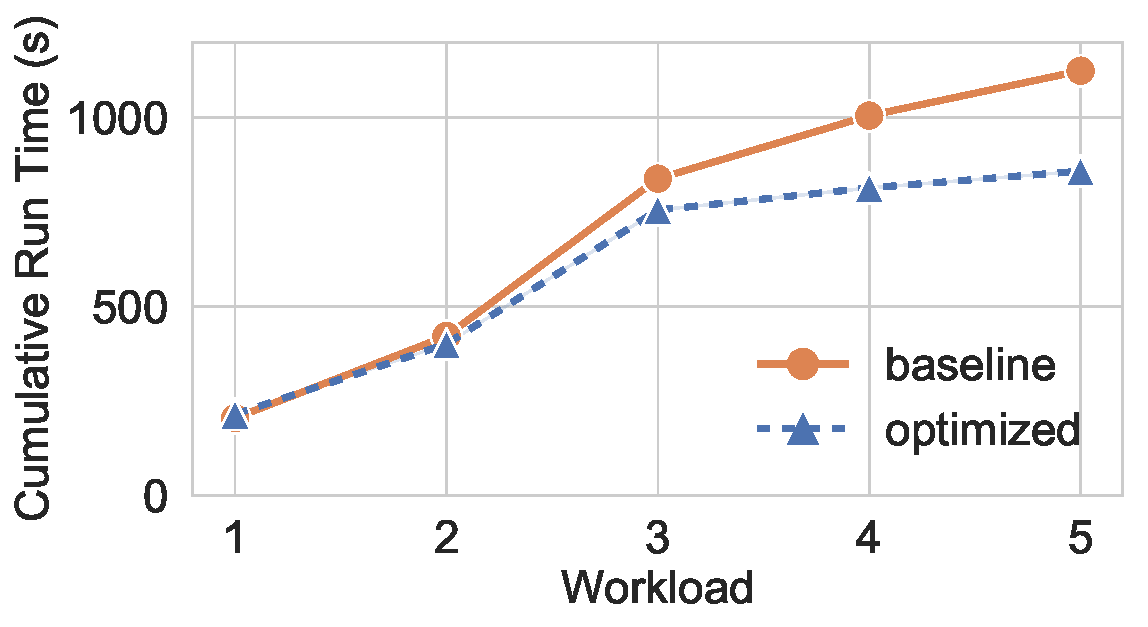
\includegraphics[width=\linewidth]{../images/experiment-results/kaggle_home_credit/execution_time/different_workloads}
 \resizebox{\columnwidth}{!}{%
%% Creator: Matplotlib, PGF backend
%%
%% To include the figure in your LaTeX document, write
%%   \input{<filename>.pgf}
%%
%% Make sure the required packages are loaded in your preamble
%%   \usepackage{pgf}
%%
%% Figures using additional raster images can only be included by \input if
%% they are in the same directory as the main LaTeX file. For loading figures
%% from other directories you can use the `import` package
%%   \usepackage{import}
%% and then include the figures with
%%   \import{<path to file>}{<filename>.pgf}
%%
%% Matplotlib used the following preamble
%%   \usepackage{fontspec}
%%   \setmonofont{Andale Mono}
%%
\begingroup%
\makeatletter%
\begin{pgfpicture}%
\pgfpathrectangle{\pgfpointorigin}{\pgfqpoint{10.411236in}{4.246930in}}%
\pgfusepath{use as bounding box, clip}%
\begin{pgfscope}%
\pgfsetbuttcap%
\pgfsetmiterjoin%
\definecolor{currentfill}{rgb}{1.000000,1.000000,1.000000}%
\pgfsetfillcolor{currentfill}%
\pgfsetlinewidth{0.000000pt}%
\definecolor{currentstroke}{rgb}{1.000000,1.000000,1.000000}%
\pgfsetstrokecolor{currentstroke}%
\pgfsetdash{}{0pt}%
\pgfpathmoveto{\pgfqpoint{0.000000in}{0.000000in}}%
\pgfpathlineto{\pgfqpoint{10.411236in}{0.000000in}}%
\pgfpathlineto{\pgfqpoint{10.411236in}{4.246930in}}%
\pgfpathlineto{\pgfqpoint{0.000000in}{4.246930in}}%
\pgfpathclose%
\pgfusepath{fill}%
\end{pgfscope}%
\begin{pgfscope}%
\pgfsetbuttcap%
\pgfsetmiterjoin%
\definecolor{currentfill}{rgb}{1.000000,1.000000,1.000000}%
\pgfsetfillcolor{currentfill}%
\pgfsetlinewidth{0.000000pt}%
\definecolor{currentstroke}{rgb}{0.000000,0.000000,0.000000}%
\pgfsetstrokecolor{currentstroke}%
\pgfsetstrokeopacity{0.000000}%
\pgfsetdash{}{0pt}%
\pgfpathmoveto{\pgfqpoint{1.719569in}{0.998541in}}%
\pgfpathlineto{\pgfqpoint{10.244569in}{0.998541in}}%
\pgfpathlineto{\pgfqpoint{10.244569in}{4.018541in}}%
\pgfpathlineto{\pgfqpoint{1.719569in}{4.018541in}}%
\pgfpathclose%
\pgfusepath{fill}%
\end{pgfscope}%
\begin{pgfscope}%
\pgfpathrectangle{\pgfqpoint{1.719569in}{0.998541in}}{\pgfqpoint{8.525000in}{3.020000in}} %
\pgfusepath{clip}%
\pgfsetroundcap%
\pgfsetroundjoin%
\pgfsetlinewidth{0.803000pt}%
\definecolor{currentstroke}{rgb}{0.500000,0.500000,0.500000}%
\pgfsetstrokecolor{currentstroke}%
\pgfsetdash{}{0pt}%
\pgfpathmoveto{\pgfqpoint{2.107069in}{0.998541in}}%
\pgfpathlineto{\pgfqpoint{2.107069in}{4.018541in}}%
\pgfusepath{stroke}%
\end{pgfscope}%
\begin{pgfscope}%
\definecolor{textcolor}{rgb}{0.150000,0.150000,0.150000}%
\pgfsetstrokecolor{textcolor}%
\pgfsetfillcolor{textcolor}%
\pgftext[x=2.107069in,y=0.834652in,,top]{\color{textcolor}\rmfamily\fontsize{25.000000}{30.000000}\selectfont 1}%
\end{pgfscope}%
\begin{pgfscope}%
\pgfpathrectangle{\pgfqpoint{1.719569in}{0.998541in}}{\pgfqpoint{8.525000in}{3.020000in}} %
\pgfusepath{clip}%
\pgfsetroundcap%
\pgfsetroundjoin%
\pgfsetlinewidth{0.803000pt}%
\definecolor{currentstroke}{rgb}{0.500000,0.500000,0.500000}%
\pgfsetstrokecolor{currentstroke}%
\pgfsetdash{}{0pt}%
\pgfpathmoveto{\pgfqpoint{3.214212in}{0.998541in}}%
\pgfpathlineto{\pgfqpoint{3.214212in}{4.018541in}}%
\pgfusepath{stroke}%
\end{pgfscope}%
\begin{pgfscope}%
\definecolor{textcolor}{rgb}{0.150000,0.150000,0.150000}%
\pgfsetstrokecolor{textcolor}%
\pgfsetfillcolor{textcolor}%
\pgftext[x=3.214212in,y=0.834652in,,top]{\color{textcolor}\rmfamily\fontsize{25.000000}{30.000000}\selectfont 2}%
\end{pgfscope}%
\begin{pgfscope}%
\pgfpathrectangle{\pgfqpoint{1.719569in}{0.998541in}}{\pgfqpoint{8.525000in}{3.020000in}} %
\pgfusepath{clip}%
\pgfsetroundcap%
\pgfsetroundjoin%
\pgfsetlinewidth{0.803000pt}%
\definecolor{currentstroke}{rgb}{0.500000,0.500000,0.500000}%
\pgfsetstrokecolor{currentstroke}%
\pgfsetdash{}{0pt}%
\pgfpathmoveto{\pgfqpoint{4.321355in}{0.998541in}}%
\pgfpathlineto{\pgfqpoint{4.321355in}{4.018541in}}%
\pgfusepath{stroke}%
\end{pgfscope}%
\begin{pgfscope}%
\definecolor{textcolor}{rgb}{0.150000,0.150000,0.150000}%
\pgfsetstrokecolor{textcolor}%
\pgfsetfillcolor{textcolor}%
\pgftext[x=4.321355in,y=0.834652in,,top]{\color{textcolor}\rmfamily\fontsize{25.000000}{30.000000}\selectfont 3}%
\end{pgfscope}%
\begin{pgfscope}%
\pgfpathrectangle{\pgfqpoint{1.719569in}{0.998541in}}{\pgfqpoint{8.525000in}{3.020000in}} %
\pgfusepath{clip}%
\pgfsetroundcap%
\pgfsetroundjoin%
\pgfsetlinewidth{0.803000pt}%
\definecolor{currentstroke}{rgb}{0.500000,0.500000,0.500000}%
\pgfsetstrokecolor{currentstroke}%
\pgfsetdash{}{0pt}%
\pgfpathmoveto{\pgfqpoint{5.428498in}{0.998541in}}%
\pgfpathlineto{\pgfqpoint{5.428498in}{4.018541in}}%
\pgfusepath{stroke}%
\end{pgfscope}%
\begin{pgfscope}%
\definecolor{textcolor}{rgb}{0.150000,0.150000,0.150000}%
\pgfsetstrokecolor{textcolor}%
\pgfsetfillcolor{textcolor}%
\pgftext[x=5.428498in,y=0.834652in,,top]{\color{textcolor}\rmfamily\fontsize{25.000000}{30.000000}\selectfont 4}%
\end{pgfscope}%
\begin{pgfscope}%
\pgfpathrectangle{\pgfqpoint{1.719569in}{0.998541in}}{\pgfqpoint{8.525000in}{3.020000in}} %
\pgfusepath{clip}%
\pgfsetroundcap%
\pgfsetroundjoin%
\pgfsetlinewidth{0.803000pt}%
\definecolor{currentstroke}{rgb}{0.500000,0.500000,0.500000}%
\pgfsetstrokecolor{currentstroke}%
\pgfsetdash{}{0pt}%
\pgfpathmoveto{\pgfqpoint{6.535641in}{0.998541in}}%
\pgfpathlineto{\pgfqpoint{6.535641in}{4.018541in}}%
\pgfusepath{stroke}%
\end{pgfscope}%
\begin{pgfscope}%
\definecolor{textcolor}{rgb}{0.150000,0.150000,0.150000}%
\pgfsetstrokecolor{textcolor}%
\pgfsetfillcolor{textcolor}%
\pgftext[x=6.535641in,y=0.834652in,,top]{\color{textcolor}\rmfamily\fontsize{25.000000}{30.000000}\selectfont 5}%
\end{pgfscope}%
\begin{pgfscope}%
\pgfpathrectangle{\pgfqpoint{1.719569in}{0.998541in}}{\pgfqpoint{8.525000in}{3.020000in}} %
\pgfusepath{clip}%
\pgfsetroundcap%
\pgfsetroundjoin%
\pgfsetlinewidth{0.803000pt}%
\definecolor{currentstroke}{rgb}{0.500000,0.500000,0.500000}%
\pgfsetstrokecolor{currentstroke}%
\pgfsetdash{}{0pt}%
\pgfpathmoveto{\pgfqpoint{7.642783in}{0.998541in}}%
\pgfpathlineto{\pgfqpoint{7.642783in}{4.018541in}}%
\pgfusepath{stroke}%
\end{pgfscope}%
\begin{pgfscope}%
\definecolor{textcolor}{rgb}{0.150000,0.150000,0.150000}%
\pgfsetstrokecolor{textcolor}%
\pgfsetfillcolor{textcolor}%
\pgftext[x=7.642783in,y=0.834652in,,top]{\color{textcolor}\rmfamily\fontsize{25.000000}{30.000000}\selectfont 6}%
\end{pgfscope}%
\begin{pgfscope}%
\pgfpathrectangle{\pgfqpoint{1.719569in}{0.998541in}}{\pgfqpoint{8.525000in}{3.020000in}} %
\pgfusepath{clip}%
\pgfsetroundcap%
\pgfsetroundjoin%
\pgfsetlinewidth{0.803000pt}%
\definecolor{currentstroke}{rgb}{0.500000,0.500000,0.500000}%
\pgfsetstrokecolor{currentstroke}%
\pgfsetdash{}{0pt}%
\pgfpathmoveto{\pgfqpoint{8.749926in}{0.998541in}}%
\pgfpathlineto{\pgfqpoint{8.749926in}{4.018541in}}%
\pgfusepath{stroke}%
\end{pgfscope}%
\begin{pgfscope}%
\definecolor{textcolor}{rgb}{0.150000,0.150000,0.150000}%
\pgfsetstrokecolor{textcolor}%
\pgfsetfillcolor{textcolor}%
\pgftext[x=8.749926in,y=0.834652in,,top]{\color{textcolor}\rmfamily\fontsize{25.000000}{30.000000}\selectfont 7}%
\end{pgfscope}%
\begin{pgfscope}%
\pgfpathrectangle{\pgfqpoint{1.719569in}{0.998541in}}{\pgfqpoint{8.525000in}{3.020000in}} %
\pgfusepath{clip}%
\pgfsetroundcap%
\pgfsetroundjoin%
\pgfsetlinewidth{0.803000pt}%
\definecolor{currentstroke}{rgb}{0.500000,0.500000,0.500000}%
\pgfsetstrokecolor{currentstroke}%
\pgfsetdash{}{0pt}%
\pgfpathmoveto{\pgfqpoint{9.857069in}{0.998541in}}%
\pgfpathlineto{\pgfqpoint{9.857069in}{4.018541in}}%
\pgfusepath{stroke}%
\end{pgfscope}%
\begin{pgfscope}%
\definecolor{textcolor}{rgb}{0.150000,0.150000,0.150000}%
\pgfsetstrokecolor{textcolor}%
\pgfsetfillcolor{textcolor}%
\pgftext[x=9.857069in,y=0.834652in,,top]{\color{textcolor}\rmfamily\fontsize{25.000000}{30.000000}\selectfont 8}%
\end{pgfscope}%
\begin{pgfscope}%
\definecolor{textcolor}{rgb}{0.150000,0.150000,0.150000}%
\pgfsetstrokecolor{textcolor}%
\pgfsetfillcolor{textcolor}%
\pgftext[x=5.982069in,y=0.470417in,,top]{\color{textcolor}\rmfamily\fontsize{30.000000}{36.000000}\selectfont Workload}%
\end{pgfscope}%
\begin{pgfscope}%
\pgfpathrectangle{\pgfqpoint{1.719569in}{0.998541in}}{\pgfqpoint{8.525000in}{3.020000in}} %
\pgfusepath{clip}%
\pgfsetroundcap%
\pgfsetroundjoin%
\pgfsetlinewidth{0.803000pt}%
\definecolor{currentstroke}{rgb}{0.500000,0.500000,0.500000}%
\pgfsetstrokecolor{currentstroke}%
\pgfsetdash{}{0pt}%
\pgfpathmoveto{\pgfqpoint{1.719569in}{0.998541in}}%
\pgfpathlineto{\pgfqpoint{10.244569in}{0.998541in}}%
\pgfusepath{stroke}%
\end{pgfscope}%
\begin{pgfscope}%
\definecolor{textcolor}{rgb}{0.150000,0.150000,0.150000}%
\pgfsetstrokecolor{textcolor}%
\pgfsetfillcolor{textcolor}%
\pgftext[x=1.396305in,y=0.878055in,left,base]{\color{textcolor}\rmfamily\fontsize{25.000000}{30.000000}\selectfont 0}%
\end{pgfscope}%
\begin{pgfscope}%
\pgfpathrectangle{\pgfqpoint{1.719569in}{0.998541in}}{\pgfqpoint{8.525000in}{3.020000in}} %
\pgfusepath{clip}%
\pgfsetroundcap%
\pgfsetroundjoin%
\pgfsetlinewidth{0.803000pt}%
\definecolor{currentstroke}{rgb}{0.500000,0.500000,0.500000}%
\pgfsetstrokecolor{currentstroke}%
\pgfsetdash{}{0pt}%
\pgfpathmoveto{\pgfqpoint{1.719569in}{1.753541in}}%
\pgfpathlineto{\pgfqpoint{10.244569in}{1.753541in}}%
\pgfusepath{stroke}%
\end{pgfscope}%
\begin{pgfscope}%
\definecolor{textcolor}{rgb}{0.150000,0.150000,0.150000}%
\pgfsetstrokecolor{textcolor}%
\pgfsetfillcolor{textcolor}%
\pgftext[x=1.077555in,y=1.633055in,left,base]{\color{textcolor}\rmfamily\fontsize{25.000000}{30.000000}\selectfont 500}%
\end{pgfscope}%
\begin{pgfscope}%
\pgfpathrectangle{\pgfqpoint{1.719569in}{0.998541in}}{\pgfqpoint{8.525000in}{3.020000in}} %
\pgfusepath{clip}%
\pgfsetroundcap%
\pgfsetroundjoin%
\pgfsetlinewidth{0.803000pt}%
\definecolor{currentstroke}{rgb}{0.500000,0.500000,0.500000}%
\pgfsetstrokecolor{currentstroke}%
\pgfsetdash{}{0pt}%
\pgfpathmoveto{\pgfqpoint{1.719569in}{2.508541in}}%
\pgfpathlineto{\pgfqpoint{10.244569in}{2.508541in}}%
\pgfusepath{stroke}%
\end{pgfscope}%
\begin{pgfscope}%
\definecolor{textcolor}{rgb}{0.150000,0.150000,0.150000}%
\pgfsetstrokecolor{textcolor}%
\pgfsetfillcolor{textcolor}%
\pgftext[x=1.227902in,y=2.388055in,left,base]{\color{textcolor}\rmfamily\fontsize{25.000000}{30.000000}\selectfont 1k}%
\end{pgfscope}%
\begin{pgfscope}%
\pgfpathrectangle{\pgfqpoint{1.719569in}{0.998541in}}{\pgfqpoint{8.525000in}{3.020000in}} %
\pgfusepath{clip}%
\pgfsetroundcap%
\pgfsetroundjoin%
\pgfsetlinewidth{0.803000pt}%
\definecolor{currentstroke}{rgb}{0.500000,0.500000,0.500000}%
\pgfsetstrokecolor{currentstroke}%
\pgfsetdash{}{0pt}%
\pgfpathmoveto{\pgfqpoint{1.719569in}{3.263541in}}%
\pgfpathlineto{\pgfqpoint{10.244569in}{3.263541in}}%
\pgfusepath{stroke}%
\end{pgfscope}%
\begin{pgfscope}%
\definecolor{textcolor}{rgb}{0.150000,0.150000,0.150000}%
\pgfsetstrokecolor{textcolor}%
\pgfsetfillcolor{textcolor}%
\pgftext[x=0.981722in,y=3.143055in,left,base]{\color{textcolor}\rmfamily\fontsize{25.000000}{30.000000}\selectfont 1.5k}%
\end{pgfscope}%
\begin{pgfscope}%
\pgfpathrectangle{\pgfqpoint{1.719569in}{0.998541in}}{\pgfqpoint{8.525000in}{3.020000in}} %
\pgfusepath{clip}%
\pgfsetroundcap%
\pgfsetroundjoin%
\pgfsetlinewidth{0.803000pt}%
\definecolor{currentstroke}{rgb}{0.500000,0.500000,0.500000}%
\pgfsetstrokecolor{currentstroke}%
\pgfsetdash{}{0pt}%
\pgfpathmoveto{\pgfqpoint{1.719569in}{4.018541in}}%
\pgfpathlineto{\pgfqpoint{10.244569in}{4.018541in}}%
\pgfusepath{stroke}%
\end{pgfscope}%
\begin{pgfscope}%
\definecolor{textcolor}{rgb}{0.150000,0.150000,0.150000}%
\pgfsetstrokecolor{textcolor}%
\pgfsetfillcolor{textcolor}%
\pgftext[x=1.227902in,y=3.898055in,left,base]{\color{textcolor}\rmfamily\fontsize{25.000000}{30.000000}\selectfont 2k}%
\end{pgfscope}%
\begin{pgfscope}%
\definecolor{textcolor}{rgb}{0.150000,0.150000,0.150000}%
\pgfsetstrokecolor{textcolor}%
\pgfsetfillcolor{textcolor}%
\pgftext[x=0.366250in,y=1.484375in,left,base,rotate=90.000000]{\color{textcolor}\rmfamily\fontsize{30.000000}{36.000000}\selectfont Cumulative }%
\end{pgfscope}%
\begin{pgfscope}%
\definecolor{textcolor}{rgb}{0.150000,0.150000,0.150000}%
\pgfsetstrokecolor{textcolor}%
\pgfsetfillcolor{textcolor}%
\pgftext[x=0.822000in,y=1.374583in,left,base,rotate=90.000000]{\color{textcolor}\rmfamily\fontsize{30.000000}{36.000000}\selectfont Run Time (s)}%
\end{pgfscope}%
\begin{pgfscope}%
\pgfpathrectangle{\pgfqpoint{1.719569in}{0.998541in}}{\pgfqpoint{8.525000in}{3.020000in}} %
\pgfusepath{clip}%
\pgfsetbuttcap%
\pgfsetroundjoin%
\pgfsetlinewidth{3.011250pt}%
\definecolor{currentstroke}{rgb}{0.298039,0.447059,0.690196}%
\pgfsetstrokecolor{currentstroke}%
\pgfsetdash{}{0pt}%
\pgfpathmoveto{\pgfqpoint{2.107069in}{1.298155in}}%
\pgfpathlineto{\pgfqpoint{2.107069in}{1.302800in}}%
\pgfusepath{stroke}%
\end{pgfscope}%
\begin{pgfscope}%
\pgfpathrectangle{\pgfqpoint{1.719569in}{0.998541in}}{\pgfqpoint{8.525000in}{3.020000in}} %
\pgfusepath{clip}%
\pgfsetbuttcap%
\pgfsetroundjoin%
\pgfsetlinewidth{3.011250pt}%
\definecolor{currentstroke}{rgb}{0.298039,0.447059,0.690196}%
\pgfsetstrokecolor{currentstroke}%
\pgfsetdash{}{0pt}%
\pgfpathmoveto{\pgfqpoint{3.214212in}{1.557722in}}%
\pgfpathlineto{\pgfqpoint{3.214212in}{1.559954in}}%
\pgfusepath{stroke}%
\end{pgfscope}%
\begin{pgfscope}%
\pgfpathrectangle{\pgfqpoint{1.719569in}{0.998541in}}{\pgfqpoint{8.525000in}{3.020000in}} %
\pgfusepath{clip}%
\pgfsetbuttcap%
\pgfsetroundjoin%
\pgfsetlinewidth{3.011250pt}%
\definecolor{currentstroke}{rgb}{0.298039,0.447059,0.690196}%
\pgfsetstrokecolor{currentstroke}%
\pgfsetdash{}{0pt}%
\pgfpathmoveto{\pgfqpoint{4.321355in}{1.995520in}}%
\pgfpathlineto{\pgfqpoint{4.321355in}{2.011654in}}%
\pgfusepath{stroke}%
\end{pgfscope}%
\begin{pgfscope}%
\pgfpathrectangle{\pgfqpoint{1.719569in}{0.998541in}}{\pgfqpoint{8.525000in}{3.020000in}} %
\pgfusepath{clip}%
\pgfsetbuttcap%
\pgfsetroundjoin%
\pgfsetlinewidth{3.011250pt}%
\definecolor{currentstroke}{rgb}{0.298039,0.447059,0.690196}%
\pgfsetstrokecolor{currentstroke}%
\pgfsetdash{}{0pt}%
\pgfpathmoveto{\pgfqpoint{5.428498in}{2.091592in}}%
\pgfpathlineto{\pgfqpoint{5.428498in}{2.109871in}}%
\pgfusepath{stroke}%
\end{pgfscope}%
\begin{pgfscope}%
\pgfpathrectangle{\pgfqpoint{1.719569in}{0.998541in}}{\pgfqpoint{8.525000in}{3.020000in}} %
\pgfusepath{clip}%
\pgfsetbuttcap%
\pgfsetroundjoin%
\pgfsetlinewidth{3.011250pt}%
\definecolor{currentstroke}{rgb}{0.298039,0.447059,0.690196}%
\pgfsetstrokecolor{currentstroke}%
\pgfsetdash{}{0pt}%
\pgfpathmoveto{\pgfqpoint{6.535641in}{2.152647in}}%
\pgfpathlineto{\pgfqpoint{6.535641in}{2.173079in}}%
\pgfusepath{stroke}%
\end{pgfscope}%
\begin{pgfscope}%
\pgfpathrectangle{\pgfqpoint{1.719569in}{0.998541in}}{\pgfqpoint{8.525000in}{3.020000in}} %
\pgfusepath{clip}%
\pgfsetbuttcap%
\pgfsetroundjoin%
\pgfsetlinewidth{3.011250pt}%
\definecolor{currentstroke}{rgb}{0.298039,0.447059,0.690196}%
\pgfsetstrokecolor{currentstroke}%
\pgfsetdash{}{0pt}%
\pgfpathmoveto{\pgfqpoint{7.642783in}{2.211090in}}%
\pgfpathlineto{\pgfqpoint{7.642783in}{2.228565in}}%
\pgfusepath{stroke}%
\end{pgfscope}%
\begin{pgfscope}%
\pgfpathrectangle{\pgfqpoint{1.719569in}{0.998541in}}{\pgfqpoint{8.525000in}{3.020000in}} %
\pgfusepath{clip}%
\pgfsetbuttcap%
\pgfsetroundjoin%
\pgfsetlinewidth{3.011250pt}%
\definecolor{currentstroke}{rgb}{0.298039,0.447059,0.690196}%
\pgfsetstrokecolor{currentstroke}%
\pgfsetdash{}{0pt}%
\pgfpathmoveto{\pgfqpoint{8.749926in}{2.276306in}}%
\pgfpathlineto{\pgfqpoint{8.749926in}{2.332493in}}%
\pgfusepath{stroke}%
\end{pgfscope}%
\begin{pgfscope}%
\pgfpathrectangle{\pgfqpoint{1.719569in}{0.998541in}}{\pgfqpoint{8.525000in}{3.020000in}} %
\pgfusepath{clip}%
\pgfsetbuttcap%
\pgfsetroundjoin%
\pgfsetlinewidth{3.011250pt}%
\definecolor{currentstroke}{rgb}{0.298039,0.447059,0.690196}%
\pgfsetstrokecolor{currentstroke}%
\pgfsetdash{}{0pt}%
\pgfpathmoveto{\pgfqpoint{9.857069in}{2.371950in}}%
\pgfpathlineto{\pgfqpoint{9.857069in}{2.426205in}}%
\pgfusepath{stroke}%
\end{pgfscope}%
\begin{pgfscope}%
\pgfpathrectangle{\pgfqpoint{1.719569in}{0.998541in}}{\pgfqpoint{8.525000in}{3.020000in}} %
\pgfusepath{clip}%
\pgfsetbuttcap%
\pgfsetroundjoin%
\pgfsetlinewidth{3.011250pt}%
\definecolor{currentstroke}{rgb}{0.866667,0.517647,0.321569}%
\pgfsetstrokecolor{currentstroke}%
\pgfsetdash{}{0pt}%
\pgfpathmoveto{\pgfqpoint{2.107069in}{1.288452in}}%
\pgfpathlineto{\pgfqpoint{2.107069in}{1.291081in}}%
\pgfusepath{stroke}%
\end{pgfscope}%
\begin{pgfscope}%
\pgfpathrectangle{\pgfqpoint{1.719569in}{0.998541in}}{\pgfqpoint{8.525000in}{3.020000in}} %
\pgfusepath{clip}%
\pgfsetbuttcap%
\pgfsetroundjoin%
\pgfsetlinewidth{3.011250pt}%
\definecolor{currentstroke}{rgb}{0.866667,0.517647,0.321569}%
\pgfsetstrokecolor{currentstroke}%
\pgfsetdash{}{0pt}%
\pgfpathmoveto{\pgfqpoint{3.214212in}{1.595643in}}%
\pgfpathlineto{\pgfqpoint{3.214212in}{1.603240in}}%
\pgfusepath{stroke}%
\end{pgfscope}%
\begin{pgfscope}%
\pgfpathrectangle{\pgfqpoint{1.719569in}{0.998541in}}{\pgfqpoint{8.525000in}{3.020000in}} %
\pgfusepath{clip}%
\pgfsetbuttcap%
\pgfsetroundjoin%
\pgfsetlinewidth{3.011250pt}%
\definecolor{currentstroke}{rgb}{0.866667,0.517647,0.321569}%
\pgfsetstrokecolor{currentstroke}%
\pgfsetdash{}{0pt}%
\pgfpathmoveto{\pgfqpoint{4.321355in}{2.136968in}}%
\pgfpathlineto{\pgfqpoint{4.321355in}{2.167950in}}%
\pgfusepath{stroke}%
\end{pgfscope}%
\begin{pgfscope}%
\pgfpathrectangle{\pgfqpoint{1.719569in}{0.998541in}}{\pgfqpoint{8.525000in}{3.020000in}} %
\pgfusepath{clip}%
\pgfsetbuttcap%
\pgfsetroundjoin%
\pgfsetlinewidth{3.011250pt}%
\definecolor{currentstroke}{rgb}{0.866667,0.517647,0.321569}%
\pgfsetstrokecolor{currentstroke}%
\pgfsetdash{}{0pt}%
\pgfpathmoveto{\pgfqpoint{5.428498in}{2.377761in}}%
\pgfpathlineto{\pgfqpoint{5.428498in}{2.408796in}}%
\pgfusepath{stroke}%
\end{pgfscope}%
\begin{pgfscope}%
\pgfpathrectangle{\pgfqpoint{1.719569in}{0.998541in}}{\pgfqpoint{8.525000in}{3.020000in}} %
\pgfusepath{clip}%
\pgfsetbuttcap%
\pgfsetroundjoin%
\pgfsetlinewidth{3.011250pt}%
\definecolor{currentstroke}{rgb}{0.866667,0.517647,0.321569}%
\pgfsetstrokecolor{currentstroke}%
\pgfsetdash{}{0pt}%
\pgfpathmoveto{\pgfqpoint{6.535641in}{2.545486in}}%
\pgfpathlineto{\pgfqpoint{6.535641in}{2.577579in}}%
\pgfusepath{stroke}%
\end{pgfscope}%
\begin{pgfscope}%
\pgfpathrectangle{\pgfqpoint{1.719569in}{0.998541in}}{\pgfqpoint{8.525000in}{3.020000in}} %
\pgfusepath{clip}%
\pgfsetbuttcap%
\pgfsetroundjoin%
\pgfsetlinewidth{3.011250pt}%
\definecolor{currentstroke}{rgb}{0.866667,0.517647,0.321569}%
\pgfsetstrokecolor{currentstroke}%
\pgfsetdash{}{0pt}%
\pgfpathmoveto{\pgfqpoint{7.642783in}{2.784438in}}%
\pgfpathlineto{\pgfqpoint{7.642783in}{2.816486in}}%
\pgfusepath{stroke}%
\end{pgfscope}%
\begin{pgfscope}%
\pgfpathrectangle{\pgfqpoint{1.719569in}{0.998541in}}{\pgfqpoint{8.525000in}{3.020000in}} %
\pgfusepath{clip}%
\pgfsetbuttcap%
\pgfsetroundjoin%
\pgfsetlinewidth{3.011250pt}%
\definecolor{currentstroke}{rgb}{0.866667,0.517647,0.321569}%
\pgfsetstrokecolor{currentstroke}%
\pgfsetdash{}{0pt}%
\pgfpathmoveto{\pgfqpoint{8.749926in}{3.309539in}}%
\pgfpathlineto{\pgfqpoint{8.749926in}{3.361997in}}%
\pgfusepath{stroke}%
\end{pgfscope}%
\begin{pgfscope}%
\pgfpathrectangle{\pgfqpoint{1.719569in}{0.998541in}}{\pgfqpoint{8.525000in}{3.020000in}} %
\pgfusepath{clip}%
\pgfsetbuttcap%
\pgfsetroundjoin%
\pgfsetlinewidth{3.011250pt}%
\definecolor{currentstroke}{rgb}{0.866667,0.517647,0.321569}%
\pgfsetstrokecolor{currentstroke}%
\pgfsetdash{}{0pt}%
\pgfpathmoveto{\pgfqpoint{9.857069in}{3.697347in}}%
\pgfpathlineto{\pgfqpoint{9.857069in}{3.754186in}}%
\pgfusepath{stroke}%
\end{pgfscope}%
\begin{pgfscope}%
\pgfpathrectangle{\pgfqpoint{1.719569in}{0.998541in}}{\pgfqpoint{8.525000in}{3.020000in}} %
\pgfusepath{clip}%
\pgfsetbuttcap%
\pgfsetroundjoin%
\pgfsetlinewidth{5.018750pt}%
\definecolor{currentstroke}{rgb}{0.298039,0.447059,0.690196}%
\pgfsetstrokecolor{currentstroke}%
\pgfsetdash{{5.000000pt}{0.000000pt}}{0.000000pt}%
\pgfpathmoveto{\pgfqpoint{2.107069in}{1.300478in}}%
\pgfpathlineto{\pgfqpoint{3.214212in}{1.558838in}}%
\pgfpathlineto{\pgfqpoint{4.321355in}{2.003587in}}%
\pgfpathlineto{\pgfqpoint{5.428498in}{2.100732in}}%
\pgfpathlineto{\pgfqpoint{6.535641in}{2.162863in}}%
\pgfpathlineto{\pgfqpoint{7.642783in}{2.219827in}}%
\pgfpathlineto{\pgfqpoint{8.749926in}{2.304400in}}%
\pgfpathlineto{\pgfqpoint{9.857069in}{2.399078in}}%
\pgfusepath{stroke}%
\end{pgfscope}%
\begin{pgfscope}%
\pgfpathrectangle{\pgfqpoint{1.719569in}{0.998541in}}{\pgfqpoint{8.525000in}{3.020000in}} %
\pgfusepath{clip}%
\pgfsetbuttcap%
\pgfsetroundjoin%
\definecolor{currentfill}{rgb}{0.298039,0.447059,0.690196}%
\pgfsetfillcolor{currentfill}%
\pgfsetlinewidth{0.752812pt}%
\definecolor{currentstroke}{rgb}{1.000000,1.000000,1.000000}%
\pgfsetstrokecolor{currentstroke}%
\pgfsetdash{}{0pt}%
\pgfsys@defobject{currentmarker}{\pgfqpoint{-0.104167in}{-0.104167in}}{\pgfqpoint{0.104167in}{0.104167in}}{%
\pgfpathmoveto{\pgfqpoint{0.000000in}{-0.104167in}}%
\pgfpathcurveto{\pgfqpoint{0.027625in}{-0.104167in}}{\pgfqpoint{0.054123in}{-0.093191in}}{\pgfqpoint{0.073657in}{-0.073657in}}%
\pgfpathcurveto{\pgfqpoint{0.093191in}{-0.054123in}}{\pgfqpoint{0.104167in}{-0.027625in}}{\pgfqpoint{0.104167in}{0.000000in}}%
\pgfpathcurveto{\pgfqpoint{0.104167in}{0.027625in}}{\pgfqpoint{0.093191in}{0.054123in}}{\pgfqpoint{0.073657in}{0.073657in}}%
\pgfpathcurveto{\pgfqpoint{0.054123in}{0.093191in}}{\pgfqpoint{0.027625in}{0.104167in}}{\pgfqpoint{0.000000in}{0.104167in}}%
\pgfpathcurveto{\pgfqpoint{-0.027625in}{0.104167in}}{\pgfqpoint{-0.054123in}{0.093191in}}{\pgfqpoint{-0.073657in}{0.073657in}}%
\pgfpathcurveto{\pgfqpoint{-0.093191in}{0.054123in}}{\pgfqpoint{-0.104167in}{0.027625in}}{\pgfqpoint{-0.104167in}{0.000000in}}%
\pgfpathcurveto{\pgfqpoint{-0.104167in}{-0.027625in}}{\pgfqpoint{-0.093191in}{-0.054123in}}{\pgfqpoint{-0.073657in}{-0.073657in}}%
\pgfpathcurveto{\pgfqpoint{-0.054123in}{-0.093191in}}{\pgfqpoint{-0.027625in}{-0.104167in}}{\pgfqpoint{0.000000in}{-0.104167in}}%
\pgfpathclose%
\pgfusepath{stroke,fill}%
}%
\begin{pgfscope}%
\pgfsys@transformshift{2.107069in}{1.300478in}%
\pgfsys@useobject{currentmarker}{}%
\end{pgfscope}%
\begin{pgfscope}%
\pgfsys@transformshift{3.214212in}{1.558838in}%
\pgfsys@useobject{currentmarker}{}%
\end{pgfscope}%
\begin{pgfscope}%
\pgfsys@transformshift{4.321355in}{2.003587in}%
\pgfsys@useobject{currentmarker}{}%
\end{pgfscope}%
\begin{pgfscope}%
\pgfsys@transformshift{5.428498in}{2.100732in}%
\pgfsys@useobject{currentmarker}{}%
\end{pgfscope}%
\begin{pgfscope}%
\pgfsys@transformshift{6.535641in}{2.162863in}%
\pgfsys@useobject{currentmarker}{}%
\end{pgfscope}%
\begin{pgfscope}%
\pgfsys@transformshift{7.642783in}{2.219827in}%
\pgfsys@useobject{currentmarker}{}%
\end{pgfscope}%
\begin{pgfscope}%
\pgfsys@transformshift{8.749926in}{2.304400in}%
\pgfsys@useobject{currentmarker}{}%
\end{pgfscope}%
\begin{pgfscope}%
\pgfsys@transformshift{9.857069in}{2.399078in}%
\pgfsys@useobject{currentmarker}{}%
\end{pgfscope}%
\end{pgfscope}%
\begin{pgfscope}%
\pgfpathrectangle{\pgfqpoint{1.719569in}{0.998541in}}{\pgfqpoint{8.525000in}{3.020000in}} %
\pgfusepath{clip}%
\pgfsetbuttcap%
\pgfsetroundjoin%
\pgfsetlinewidth{5.018750pt}%
\definecolor{currentstroke}{rgb}{0.866667,0.517647,0.321569}%
\pgfsetstrokecolor{currentstroke}%
\pgfsetdash{{15.000000pt}{5.000000pt}}{0.000000pt}%
\pgfpathmoveto{\pgfqpoint{2.107069in}{1.289767in}}%
\pgfpathlineto{\pgfqpoint{3.214212in}{1.599441in}}%
\pgfpathlineto{\pgfqpoint{4.321355in}{2.152459in}}%
\pgfpathlineto{\pgfqpoint{5.428498in}{2.393278in}}%
\pgfpathlineto{\pgfqpoint{6.535641in}{2.561532in}}%
\pgfpathlineto{\pgfqpoint{7.642783in}{2.800462in}}%
\pgfpathlineto{\pgfqpoint{8.749926in}{3.335768in}}%
\pgfpathlineto{\pgfqpoint{9.857069in}{3.725766in}}%
\pgfusepath{stroke}%
\end{pgfscope}%
\begin{pgfscope}%
\pgfpathrectangle{\pgfqpoint{1.719569in}{0.998541in}}{\pgfqpoint{8.525000in}{3.020000in}} %
\pgfusepath{clip}%
\pgfsetbuttcap%
\pgfsetmiterjoin%
\definecolor{currentfill}{rgb}{0.866667,0.517647,0.321569}%
\pgfsetfillcolor{currentfill}%
\pgfsetlinewidth{0.752812pt}%
\definecolor{currentstroke}{rgb}{1.000000,1.000000,1.000000}%
\pgfsetstrokecolor{currentstroke}%
\pgfsetdash{}{0pt}%
\pgfsys@defobject{currentmarker}{\pgfqpoint{-0.104167in}{-0.104167in}}{\pgfqpoint{0.104167in}{0.104167in}}{%
\pgfpathmoveto{\pgfqpoint{0.000000in}{0.104167in}}%
\pgfpathlineto{\pgfqpoint{-0.104167in}{-0.104167in}}%
\pgfpathlineto{\pgfqpoint{0.104167in}{-0.104167in}}%
\pgfpathclose%
\pgfusepath{stroke,fill}%
}%
\begin{pgfscope}%
\pgfsys@transformshift{2.107069in}{1.289767in}%
\pgfsys@useobject{currentmarker}{}%
\end{pgfscope}%
\begin{pgfscope}%
\pgfsys@transformshift{3.214212in}{1.599441in}%
\pgfsys@useobject{currentmarker}{}%
\end{pgfscope}%
\begin{pgfscope}%
\pgfsys@transformshift{4.321355in}{2.152459in}%
\pgfsys@useobject{currentmarker}{}%
\end{pgfscope}%
\begin{pgfscope}%
\pgfsys@transformshift{5.428498in}{2.393278in}%
\pgfsys@useobject{currentmarker}{}%
\end{pgfscope}%
\begin{pgfscope}%
\pgfsys@transformshift{6.535641in}{2.561532in}%
\pgfsys@useobject{currentmarker}{}%
\end{pgfscope}%
\begin{pgfscope}%
\pgfsys@transformshift{7.642783in}{2.800462in}%
\pgfsys@useobject{currentmarker}{}%
\end{pgfscope}%
\begin{pgfscope}%
\pgfsys@transformshift{8.749926in}{3.335768in}%
\pgfsys@useobject{currentmarker}{}%
\end{pgfscope}%
\begin{pgfscope}%
\pgfsys@transformshift{9.857069in}{3.725766in}%
\pgfsys@useobject{currentmarker}{}%
\end{pgfscope}%
\end{pgfscope}%
\begin{pgfscope}%
\pgfsetrectcap%
\pgfsetmiterjoin%
\pgfsetlinewidth{1.003750pt}%
\definecolor{currentstroke}{rgb}{0.800000,0.800000,0.800000}%
\pgfsetstrokecolor{currentstroke}%
\pgfsetdash{}{0pt}%
\pgfpathmoveto{\pgfqpoint{1.719569in}{0.998541in}}%
\pgfpathlineto{\pgfqpoint{1.719569in}{4.018541in}}%
\pgfusepath{stroke}%
\end{pgfscope}%
\begin{pgfscope}%
\pgfsetrectcap%
\pgfsetmiterjoin%
\pgfsetlinewidth{1.003750pt}%
\definecolor{currentstroke}{rgb}{0.800000,0.800000,0.800000}%
\pgfsetstrokecolor{currentstroke}%
\pgfsetdash{}{0pt}%
\pgfpathmoveto{\pgfqpoint{10.244569in}{0.998541in}}%
\pgfpathlineto{\pgfqpoint{10.244569in}{4.018541in}}%
\pgfusepath{stroke}%
\end{pgfscope}%
\begin{pgfscope}%
\pgfsetrectcap%
\pgfsetmiterjoin%
\pgfsetlinewidth{1.003750pt}%
\definecolor{currentstroke}{rgb}{0.800000,0.800000,0.800000}%
\pgfsetstrokecolor{currentstroke}%
\pgfsetdash{}{0pt}%
\pgfpathmoveto{\pgfqpoint{1.719569in}{0.998541in}}%
\pgfpathlineto{\pgfqpoint{10.244569in}{0.998541in}}%
\pgfusepath{stroke}%
\end{pgfscope}%
\begin{pgfscope}%
\pgfsetrectcap%
\pgfsetmiterjoin%
\pgfsetlinewidth{1.003750pt}%
\definecolor{currentstroke}{rgb}{0.800000,0.800000,0.800000}%
\pgfsetstrokecolor{currentstroke}%
\pgfsetdash{}{0pt}%
\pgfpathmoveto{\pgfqpoint{1.719569in}{4.018541in}}%
\pgfpathlineto{\pgfqpoint{10.244569in}{4.018541in}}%
\pgfusepath{stroke}%
\end{pgfscope}%
\begin{pgfscope}%
\pgfsetbuttcap%
\pgfsetroundjoin%
\pgfsetlinewidth{3.011250pt}%
\definecolor{currentstroke}{rgb}{0.298039,0.447059,0.690196}%
\pgfsetstrokecolor{currentstroke}%
\pgfsetdash{{3.000000pt}{0.000000pt}}{0.000000pt}%
\pgfpathmoveto{\pgfqpoint{4.678771in}{3.886513in}}%
\pgfpathlineto{\pgfqpoint{5.373215in}{3.886513in}}%
\pgfusepath{stroke}%
\end{pgfscope}%
\begin{pgfscope}%
\pgfsetbuttcap%
\pgfsetroundjoin%
\definecolor{currentfill}{rgb}{0.298039,0.447059,0.690196}%
\pgfsetfillcolor{currentfill}%
\pgfsetlinewidth{0.000000pt}%
\definecolor{currentstroke}{rgb}{0.298039,0.447059,0.690196}%
\pgfsetstrokecolor{currentstroke}%
\pgfsetdash{}{0pt}%
\pgfsys@defobject{currentmarker}{\pgfqpoint{-0.104167in}{-0.104167in}}{\pgfqpoint{0.104167in}{0.104167in}}{%
\pgfpathmoveto{\pgfqpoint{0.000000in}{-0.104167in}}%
\pgfpathcurveto{\pgfqpoint{0.027625in}{-0.104167in}}{\pgfqpoint{0.054123in}{-0.093191in}}{\pgfqpoint{0.073657in}{-0.073657in}}%
\pgfpathcurveto{\pgfqpoint{0.093191in}{-0.054123in}}{\pgfqpoint{0.104167in}{-0.027625in}}{\pgfqpoint{0.104167in}{0.000000in}}%
\pgfpathcurveto{\pgfqpoint{0.104167in}{0.027625in}}{\pgfqpoint{0.093191in}{0.054123in}}{\pgfqpoint{0.073657in}{0.073657in}}%
\pgfpathcurveto{\pgfqpoint{0.054123in}{0.093191in}}{\pgfqpoint{0.027625in}{0.104167in}}{\pgfqpoint{0.000000in}{0.104167in}}%
\pgfpathcurveto{\pgfqpoint{-0.027625in}{0.104167in}}{\pgfqpoint{-0.054123in}{0.093191in}}{\pgfqpoint{-0.073657in}{0.073657in}}%
\pgfpathcurveto{\pgfqpoint{-0.093191in}{0.054123in}}{\pgfqpoint{-0.104167in}{0.027625in}}{\pgfqpoint{-0.104167in}{0.000000in}}%
\pgfpathcurveto{\pgfqpoint{-0.104167in}{-0.027625in}}{\pgfqpoint{-0.093191in}{-0.054123in}}{\pgfqpoint{-0.073657in}{-0.073657in}}%
\pgfpathcurveto{\pgfqpoint{-0.054123in}{-0.093191in}}{\pgfqpoint{-0.027625in}{-0.104167in}}{\pgfqpoint{0.000000in}{-0.104167in}}%
\pgfpathclose%
\pgfusepath{fill}%
}%
\begin{pgfscope}%
\pgfsys@transformshift{5.025993in}{3.886513in}%
\pgfsys@useobject{currentmarker}{}%
\end{pgfscope}%
\end{pgfscope}%
\begin{pgfscope}%
\definecolor{textcolor}{rgb}{0.150000,0.150000,0.150000}%
\pgfsetstrokecolor{textcolor}%
\pgfsetfillcolor{textcolor}%
\pgftext[x=5.407937in,y=3.764986in,left,base]{\color{textcolor}\rmfamily\fontsize{25.000000}{30.000000}\selectfont CO}%
\end{pgfscope}%
\begin{pgfscope}%
\pgfsetbuttcap%
\pgfsetroundjoin%
\pgfsetlinewidth{3.011250pt}%
\definecolor{currentstroke}{rgb}{0.866667,0.517647,0.321569}%
\pgfsetstrokecolor{currentstroke}%
\pgfsetdash{{9.000000pt}{3.000000pt}}{0.000000pt}%
\pgfpathmoveto{\pgfqpoint{6.063493in}{3.886513in}}%
\pgfpathlineto{\pgfqpoint{6.757937in}{3.886513in}}%
\pgfusepath{stroke}%
\end{pgfscope}%
\begin{pgfscope}%
\pgfsetbuttcap%
\pgfsetmiterjoin%
\definecolor{currentfill}{rgb}{0.866667,0.517647,0.321569}%
\pgfsetfillcolor{currentfill}%
\pgfsetlinewidth{0.000000pt}%
\definecolor{currentstroke}{rgb}{0.866667,0.517647,0.321569}%
\pgfsetstrokecolor{currentstroke}%
\pgfsetdash{}{0pt}%
\pgfsys@defobject{currentmarker}{\pgfqpoint{-0.104167in}{-0.104167in}}{\pgfqpoint{0.104167in}{0.104167in}}{%
\pgfpathmoveto{\pgfqpoint{0.000000in}{0.104167in}}%
\pgfpathlineto{\pgfqpoint{-0.104167in}{-0.104167in}}%
\pgfpathlineto{\pgfqpoint{0.104167in}{-0.104167in}}%
\pgfpathclose%
\pgfusepath{fill}%
}%
\begin{pgfscope}%
\pgfsys@transformshift{6.410715in}{3.886513in}%
\pgfsys@useobject{currentmarker}{}%
\end{pgfscope}%
\end{pgfscope}%
\begin{pgfscope}%
\definecolor{textcolor}{rgb}{0.150000,0.150000,0.150000}%
\pgfsetstrokecolor{textcolor}%
\pgfsetfillcolor{textcolor}%
\pgftext[x=6.792659in,y=3.764986in,left,base]{\color{textcolor}\rmfamily\fontsize{25.000000}{30.000000}\selectfont KG}%
\end{pgfscope}%
\end{pgfpicture}%
\makeatother%
\endgroup%
%
}
\caption{Execution of Kaggle workloads in sequence}
\end{subfigure}
\caption{Execution of Kaggle workloads (materialization budget = 32 GB). KG = Kaggle's infrastructure (our baseline), CO = Collaborative Optimizer.}
\label{exp-reuse-kaggle-same-workload}
\end{figure}

Figure \ref{exp-reuse-kaggle-same-workload}(d) shows the cumulative run-time of executing the workloads of Table \ref{kaggle-workload} in sequence.
This corresponds to a real scenario, where after some scripts in a collaborative environment gain popularity, e.g., Workloads 1-3, other users modify and try to improve them, e.g, Workloads 4-8.
The experiment shows that optimize even a single execution of each workload decreases the cumulative run-time by half.
In a real collaborative environment, there are hundreds of more modified scripts and possibly thousands of repeated execution of such scripts, resulting in 1000s of hours of reduction in the cumulative run-time.

\subsection{Materialization}
In this set of experiments, we show the impact of our materialization algorithms on the total size of the stored artifacts and total run-time of the workloads.
We run the workloads of Table \ref{kaggle-workload} under different materialization budgets using both our heuristics-based and storage-aware materialization algorithms.

Figures \ref{exp-sa-vs-simple-size}(a)-(d) show the real size of the stored artifacts under different materialization budgets.
For the heuristics-based algorithm, the maximum real size is always capped at the budget.
However, in the storage-aware algorithm, we observe that the real size of the stored artifacts can reach up to 8 times the budget.
With a materialization budget of 8 GB, the storage-aware algorithm materializes almost half of the artifacts.
When the materialization budget is more than 8 GB, storage-aware materialized nearly all the artifacts.
This indicates that there is considerable overlap between the artifacts of ML workloads.
By deduplicating the artifacts, our storage-aware materialization algorithm can materialize more artifacts.
As a result, the storage-aware achieves a much smaller total run-time when compared with the heuristics-based materialization.

\begin{figure}
\begin{subfigure}[b]{0.5\linewidth}
\centering
 \resizebox{\columnwidth}{!}{%
%% Creator: Matplotlib, PGF backend
%%
%% To include the figure in your LaTeX document, write
%%   \input{<filename>.pgf}
%%
%% Make sure the required packages are loaded in your preamble
%%   \usepackage{pgf}
%%
%% Figures using additional raster images can only be included by \input if
%% they are in the same directory as the main LaTeX file. For loading figures
%% from other directories you can use the `import` package
%%   \usepackage{import}
%% and then include the figures with
%%   \import{<path to file>}{<filename>.pgf}
%%
%% Matplotlib used the following preamble
%%   \usepackage{fontspec}
%%   \setmonofont{Andale Mono}
%%
\begingroup%
\makeatletter%
\begin{pgfpicture}%
\pgfpathrectangle{\pgfpointorigin}{\pgfqpoint{7.891361in}{4.902228in}}%
\pgfusepath{use as bounding box, clip}%
\begin{pgfscope}%
\pgfsetbuttcap%
\pgfsetmiterjoin%
\definecolor{currentfill}{rgb}{1.000000,1.000000,1.000000}%
\pgfsetfillcolor{currentfill}%
\pgfsetlinewidth{0.000000pt}%
\definecolor{currentstroke}{rgb}{1.000000,1.000000,1.000000}%
\pgfsetstrokecolor{currentstroke}%
\pgfsetdash{}{0pt}%
\pgfpathmoveto{\pgfqpoint{0.000000in}{0.000000in}}%
\pgfpathlineto{\pgfqpoint{7.891361in}{0.000000in}}%
\pgfpathlineto{\pgfqpoint{7.891361in}{4.902228in}}%
\pgfpathlineto{\pgfqpoint{0.000000in}{4.902228in}}%
\pgfpathclose%
\pgfusepath{fill}%
\end{pgfscope}%
\begin{pgfscope}%
\pgfsetbuttcap%
\pgfsetmiterjoin%
\definecolor{currentfill}{rgb}{1.000000,1.000000,1.000000}%
\pgfsetfillcolor{currentfill}%
\pgfsetlinewidth{0.000000pt}%
\definecolor{currentstroke}{rgb}{0.000000,0.000000,0.000000}%
\pgfsetstrokecolor{currentstroke}%
\pgfsetstrokeopacity{0.000000}%
\pgfsetdash{}{0pt}%
\pgfpathmoveto{\pgfqpoint{1.524694in}{1.233139in}}%
\pgfpathlineto{\pgfqpoint{7.724694in}{1.233139in}}%
\pgfpathlineto{\pgfqpoint{7.724694in}{4.253139in}}%
\pgfpathlineto{\pgfqpoint{1.524694in}{4.253139in}}%
\pgfpathclose%
\pgfusepath{fill}%
\end{pgfscope}%
\begin{pgfscope}%
\pgfpathrectangle{\pgfqpoint{1.524694in}{1.233139in}}{\pgfqpoint{6.200000in}{3.020000in}} %
\pgfusepath{clip}%
\pgfsetroundcap%
\pgfsetroundjoin%
\pgfsetlinewidth{0.803000pt}%
\definecolor{currentstroke}{rgb}{0.500000,0.500000,0.500000}%
\pgfsetstrokecolor{currentstroke}%
\pgfsetdash{}{0pt}%
\pgfpathmoveto{\pgfqpoint{1.806512in}{1.233139in}}%
\pgfpathlineto{\pgfqpoint{1.806512in}{4.253139in}}%
\pgfusepath{stroke}%
\end{pgfscope}%
\begin{pgfscope}%
\definecolor{textcolor}{rgb}{0.150000,0.150000,0.150000}%
\pgfsetstrokecolor{textcolor}%
\pgfsetfillcolor{textcolor}%
\pgftext[x=1.806512in,y=1.069250in,,top]{\color{textcolor}\rmfamily\fontsize{34.000000}{40.800000}\selectfont 1}%
\end{pgfscope}%
\begin{pgfscope}%
\pgfpathrectangle{\pgfqpoint{1.524694in}{1.233139in}}{\pgfqpoint{6.200000in}{3.020000in}} %
\pgfusepath{clip}%
\pgfsetroundcap%
\pgfsetroundjoin%
\pgfsetlinewidth{0.803000pt}%
\definecolor{currentstroke}{rgb}{0.500000,0.500000,0.500000}%
\pgfsetstrokecolor{currentstroke}%
\pgfsetdash{}{0pt}%
\pgfpathmoveto{\pgfqpoint{2.611707in}{1.233139in}}%
\pgfpathlineto{\pgfqpoint{2.611707in}{4.253139in}}%
\pgfusepath{stroke}%
\end{pgfscope}%
\begin{pgfscope}%
\definecolor{textcolor}{rgb}{0.150000,0.150000,0.150000}%
\pgfsetstrokecolor{textcolor}%
\pgfsetfillcolor{textcolor}%
\pgftext[x=2.611707in,y=1.069250in,,top]{\color{textcolor}\rmfamily\fontsize{34.000000}{40.800000}\selectfont 2}%
\end{pgfscope}%
\begin{pgfscope}%
\pgfpathrectangle{\pgfqpoint{1.524694in}{1.233139in}}{\pgfqpoint{6.200000in}{3.020000in}} %
\pgfusepath{clip}%
\pgfsetroundcap%
\pgfsetroundjoin%
\pgfsetlinewidth{0.803000pt}%
\definecolor{currentstroke}{rgb}{0.500000,0.500000,0.500000}%
\pgfsetstrokecolor{currentstroke}%
\pgfsetdash{}{0pt}%
\pgfpathmoveto{\pgfqpoint{3.416902in}{1.233139in}}%
\pgfpathlineto{\pgfqpoint{3.416902in}{4.253139in}}%
\pgfusepath{stroke}%
\end{pgfscope}%
\begin{pgfscope}%
\definecolor{textcolor}{rgb}{0.150000,0.150000,0.150000}%
\pgfsetstrokecolor{textcolor}%
\pgfsetfillcolor{textcolor}%
\pgftext[x=3.416902in,y=1.069250in,,top]{\color{textcolor}\rmfamily\fontsize{34.000000}{40.800000}\selectfont 3}%
\end{pgfscope}%
\begin{pgfscope}%
\pgfpathrectangle{\pgfqpoint{1.524694in}{1.233139in}}{\pgfqpoint{6.200000in}{3.020000in}} %
\pgfusepath{clip}%
\pgfsetroundcap%
\pgfsetroundjoin%
\pgfsetlinewidth{0.803000pt}%
\definecolor{currentstroke}{rgb}{0.500000,0.500000,0.500000}%
\pgfsetstrokecolor{currentstroke}%
\pgfsetdash{}{0pt}%
\pgfpathmoveto{\pgfqpoint{4.222097in}{1.233139in}}%
\pgfpathlineto{\pgfqpoint{4.222097in}{4.253139in}}%
\pgfusepath{stroke}%
\end{pgfscope}%
\begin{pgfscope}%
\definecolor{textcolor}{rgb}{0.150000,0.150000,0.150000}%
\pgfsetstrokecolor{textcolor}%
\pgfsetfillcolor{textcolor}%
\pgftext[x=4.222097in,y=1.069250in,,top]{\color{textcolor}\rmfamily\fontsize{34.000000}{40.800000}\selectfont 4}%
\end{pgfscope}%
\begin{pgfscope}%
\pgfpathrectangle{\pgfqpoint{1.524694in}{1.233139in}}{\pgfqpoint{6.200000in}{3.020000in}} %
\pgfusepath{clip}%
\pgfsetroundcap%
\pgfsetroundjoin%
\pgfsetlinewidth{0.803000pt}%
\definecolor{currentstroke}{rgb}{0.500000,0.500000,0.500000}%
\pgfsetstrokecolor{currentstroke}%
\pgfsetdash{}{0pt}%
\pgfpathmoveto{\pgfqpoint{5.027292in}{1.233139in}}%
\pgfpathlineto{\pgfqpoint{5.027292in}{4.253139in}}%
\pgfusepath{stroke}%
\end{pgfscope}%
\begin{pgfscope}%
\definecolor{textcolor}{rgb}{0.150000,0.150000,0.150000}%
\pgfsetstrokecolor{textcolor}%
\pgfsetfillcolor{textcolor}%
\pgftext[x=5.027292in,y=1.069250in,,top]{\color{textcolor}\rmfamily\fontsize{34.000000}{40.800000}\selectfont 5}%
\end{pgfscope}%
\begin{pgfscope}%
\pgfpathrectangle{\pgfqpoint{1.524694in}{1.233139in}}{\pgfqpoint{6.200000in}{3.020000in}} %
\pgfusepath{clip}%
\pgfsetroundcap%
\pgfsetroundjoin%
\pgfsetlinewidth{0.803000pt}%
\definecolor{currentstroke}{rgb}{0.500000,0.500000,0.500000}%
\pgfsetstrokecolor{currentstroke}%
\pgfsetdash{}{0pt}%
\pgfpathmoveto{\pgfqpoint{5.832487in}{1.233139in}}%
\pgfpathlineto{\pgfqpoint{5.832487in}{4.253139in}}%
\pgfusepath{stroke}%
\end{pgfscope}%
\begin{pgfscope}%
\definecolor{textcolor}{rgb}{0.150000,0.150000,0.150000}%
\pgfsetstrokecolor{textcolor}%
\pgfsetfillcolor{textcolor}%
\pgftext[x=5.832487in,y=1.069250in,,top]{\color{textcolor}\rmfamily\fontsize{34.000000}{40.800000}\selectfont 6}%
\end{pgfscope}%
\begin{pgfscope}%
\pgfpathrectangle{\pgfqpoint{1.524694in}{1.233139in}}{\pgfqpoint{6.200000in}{3.020000in}} %
\pgfusepath{clip}%
\pgfsetroundcap%
\pgfsetroundjoin%
\pgfsetlinewidth{0.803000pt}%
\definecolor{currentstroke}{rgb}{0.500000,0.500000,0.500000}%
\pgfsetstrokecolor{currentstroke}%
\pgfsetdash{}{0pt}%
\pgfpathmoveto{\pgfqpoint{6.637681in}{1.233139in}}%
\pgfpathlineto{\pgfqpoint{6.637681in}{4.253139in}}%
\pgfusepath{stroke}%
\end{pgfscope}%
\begin{pgfscope}%
\definecolor{textcolor}{rgb}{0.150000,0.150000,0.150000}%
\pgfsetstrokecolor{textcolor}%
\pgfsetfillcolor{textcolor}%
\pgftext[x=6.637681in,y=1.069250in,,top]{\color{textcolor}\rmfamily\fontsize{34.000000}{40.800000}\selectfont 7}%
\end{pgfscope}%
\begin{pgfscope}%
\pgfpathrectangle{\pgfqpoint{1.524694in}{1.233139in}}{\pgfqpoint{6.200000in}{3.020000in}} %
\pgfusepath{clip}%
\pgfsetroundcap%
\pgfsetroundjoin%
\pgfsetlinewidth{0.803000pt}%
\definecolor{currentstroke}{rgb}{0.500000,0.500000,0.500000}%
\pgfsetstrokecolor{currentstroke}%
\pgfsetdash{}{0pt}%
\pgfpathmoveto{\pgfqpoint{7.442876in}{1.233139in}}%
\pgfpathlineto{\pgfqpoint{7.442876in}{4.253139in}}%
\pgfusepath{stroke}%
\end{pgfscope}%
\begin{pgfscope}%
\definecolor{textcolor}{rgb}{0.150000,0.150000,0.150000}%
\pgfsetstrokecolor{textcolor}%
\pgfsetfillcolor{textcolor}%
\pgftext[x=7.442876in,y=1.069250in,,top]{\color{textcolor}\rmfamily\fontsize{34.000000}{40.800000}\selectfont 8}%
\end{pgfscope}%
\begin{pgfscope}%
\definecolor{textcolor}{rgb}{0.150000,0.150000,0.150000}%
\pgfsetstrokecolor{textcolor}%
\pgfsetfillcolor{textcolor}%
\pgftext[x=4.624694in,y=0.593889in,,top]{\color{textcolor}\rmfamily\fontsize{40.000000}{48.000000}\selectfont Workload}%
\end{pgfscope}%
\begin{pgfscope}%
\pgfpathrectangle{\pgfqpoint{1.524694in}{1.233139in}}{\pgfqpoint{6.200000in}{3.020000in}} %
\pgfusepath{clip}%
\pgfsetroundcap%
\pgfsetroundjoin%
\pgfsetlinewidth{0.803000pt}%
\definecolor{currentstroke}{rgb}{0.500000,0.500000,0.500000}%
\pgfsetstrokecolor{currentstroke}%
\pgfsetdash{}{0pt}%
\pgfpathmoveto{\pgfqpoint{1.524694in}{1.233139in}}%
\pgfpathlineto{\pgfqpoint{7.724694in}{1.233139in}}%
\pgfusepath{stroke}%
\end{pgfscope}%
\begin{pgfscope}%
\definecolor{textcolor}{rgb}{0.150000,0.150000,0.150000}%
\pgfsetstrokecolor{textcolor}%
\pgfsetfillcolor{textcolor}%
\pgftext[x=1.144055in,y=1.069278in,left,base]{\color{textcolor}\rmfamily\fontsize{34.000000}{40.800000}\selectfont 0}%
\end{pgfscope}%
\begin{pgfscope}%
\pgfpathrectangle{\pgfqpoint{1.524694in}{1.233139in}}{\pgfqpoint{6.200000in}{3.020000in}} %
\pgfusepath{clip}%
\pgfsetroundcap%
\pgfsetroundjoin%
\pgfsetlinewidth{0.803000pt}%
\definecolor{currentstroke}{rgb}{0.500000,0.500000,0.500000}%
\pgfsetstrokecolor{currentstroke}%
\pgfsetdash{}{0pt}%
\pgfpathmoveto{\pgfqpoint{1.524694in}{1.772424in}}%
\pgfpathlineto{\pgfqpoint{7.724694in}{1.772424in}}%
\pgfusepath{stroke}%
\end{pgfscope}%
\begin{pgfscope}%
\definecolor{textcolor}{rgb}{0.150000,0.150000,0.150000}%
\pgfsetstrokecolor{textcolor}%
\pgfsetfillcolor{textcolor}%
\pgftext[x=0.927305in,y=1.608563in,left,base]{\color{textcolor}\rmfamily\fontsize{34.000000}{40.800000}\selectfont 25}%
\end{pgfscope}%
\begin{pgfscope}%
\pgfpathrectangle{\pgfqpoint{1.524694in}{1.233139in}}{\pgfqpoint{6.200000in}{3.020000in}} %
\pgfusepath{clip}%
\pgfsetroundcap%
\pgfsetroundjoin%
\pgfsetlinewidth{0.803000pt}%
\definecolor{currentstroke}{rgb}{0.500000,0.500000,0.500000}%
\pgfsetstrokecolor{currentstroke}%
\pgfsetdash{}{0pt}%
\pgfpathmoveto{\pgfqpoint{1.524694in}{2.311710in}}%
\pgfpathlineto{\pgfqpoint{7.724694in}{2.311710in}}%
\pgfusepath{stroke}%
\end{pgfscope}%
\begin{pgfscope}%
\definecolor{textcolor}{rgb}{0.150000,0.150000,0.150000}%
\pgfsetstrokecolor{textcolor}%
\pgfsetfillcolor{textcolor}%
\pgftext[x=0.927305in,y=2.147849in,left,base]{\color{textcolor}\rmfamily\fontsize{34.000000}{40.800000}\selectfont 50}%
\end{pgfscope}%
\begin{pgfscope}%
\pgfpathrectangle{\pgfqpoint{1.524694in}{1.233139in}}{\pgfqpoint{6.200000in}{3.020000in}} %
\pgfusepath{clip}%
\pgfsetroundcap%
\pgfsetroundjoin%
\pgfsetlinewidth{0.803000pt}%
\definecolor{currentstroke}{rgb}{0.500000,0.500000,0.500000}%
\pgfsetstrokecolor{currentstroke}%
\pgfsetdash{}{0pt}%
\pgfpathmoveto{\pgfqpoint{1.524694in}{2.850996in}}%
\pgfpathlineto{\pgfqpoint{7.724694in}{2.850996in}}%
\pgfusepath{stroke}%
\end{pgfscope}%
\begin{pgfscope}%
\definecolor{textcolor}{rgb}{0.150000,0.150000,0.150000}%
\pgfsetstrokecolor{textcolor}%
\pgfsetfillcolor{textcolor}%
\pgftext[x=0.927305in,y=2.687135in,left,base]{\color{textcolor}\rmfamily\fontsize{34.000000}{40.800000}\selectfont 75}%
\end{pgfscope}%
\begin{pgfscope}%
\pgfpathrectangle{\pgfqpoint{1.524694in}{1.233139in}}{\pgfqpoint{6.200000in}{3.020000in}} %
\pgfusepath{clip}%
\pgfsetroundcap%
\pgfsetroundjoin%
\pgfsetlinewidth{0.803000pt}%
\definecolor{currentstroke}{rgb}{0.500000,0.500000,0.500000}%
\pgfsetstrokecolor{currentstroke}%
\pgfsetdash{}{0pt}%
\pgfpathmoveto{\pgfqpoint{1.524694in}{3.390282in}}%
\pgfpathlineto{\pgfqpoint{7.724694in}{3.390282in}}%
\pgfusepath{stroke}%
\end{pgfscope}%
\begin{pgfscope}%
\definecolor{textcolor}{rgb}{0.150000,0.150000,0.150000}%
\pgfsetstrokecolor{textcolor}%
\pgfsetfillcolor{textcolor}%
\pgftext[x=0.710555in,y=3.226420in,left,base]{\color{textcolor}\rmfamily\fontsize{34.000000}{40.800000}\selectfont 100}%
\end{pgfscope}%
\begin{pgfscope}%
\pgfpathrectangle{\pgfqpoint{1.524694in}{1.233139in}}{\pgfqpoint{6.200000in}{3.020000in}} %
\pgfusepath{clip}%
\pgfsetroundcap%
\pgfsetroundjoin%
\pgfsetlinewidth{0.803000pt}%
\definecolor{currentstroke}{rgb}{0.500000,0.500000,0.500000}%
\pgfsetstrokecolor{currentstroke}%
\pgfsetdash{}{0pt}%
\pgfpathmoveto{\pgfqpoint{1.524694in}{3.929567in}}%
\pgfpathlineto{\pgfqpoint{7.724694in}{3.929567in}}%
\pgfusepath{stroke}%
\end{pgfscope}%
\begin{pgfscope}%
\definecolor{textcolor}{rgb}{0.150000,0.150000,0.150000}%
\pgfsetstrokecolor{textcolor}%
\pgfsetfillcolor{textcolor}%
\pgftext[x=0.710555in,y=3.765706in,left,base]{\color{textcolor}\rmfamily\fontsize{34.000000}{40.800000}\selectfont 125}%
\end{pgfscope}%
\begin{pgfscope}%
\definecolor{textcolor}{rgb}{0.150000,0.150000,0.150000}%
\pgfsetstrokecolor{textcolor}%
\pgfsetfillcolor{textcolor}%
\pgftext[x=0.655000in,y=2.743139in,,bottom,rotate=90.000000]{\color{textcolor}\rmfamily\fontsize{40.000000}{48.000000}\selectfont Size (GB)}%
\end{pgfscope}%
\begin{pgfscope}%
\pgfpathrectangle{\pgfqpoint{1.524694in}{1.233139in}}{\pgfqpoint{6.200000in}{3.020000in}} %
\pgfusepath{clip}%
\pgfsetbuttcap%
\pgfsetroundjoin%
\definecolor{currentfill}{rgb}{0.298039,0.447059,0.690196}%
\pgfsetfillcolor{currentfill}%
\pgfsetfillopacity{0.200000}%
\pgfsetlinewidth{0.803000pt}%
\definecolor{currentstroke}{rgb}{0.298039,0.447059,0.690196}%
\pgfsetstrokecolor{currentstroke}%
\pgfsetstrokeopacity{0.200000}%
\pgfsetdash{}{0pt}%
\pgfpathmoveto{\pgfqpoint{1.806512in}{1.546546in}}%
\pgfpathlineto{\pgfqpoint{1.806512in}{1.546546in}}%
\pgfpathlineto{\pgfqpoint{2.611707in}{2.063342in}}%
\pgfpathlineto{\pgfqpoint{3.416902in}{1.769890in}}%
\pgfpathlineto{\pgfqpoint{4.222097in}{1.895014in}}%
\pgfpathlineto{\pgfqpoint{5.027292in}{2.020360in}}%
\pgfpathlineto{\pgfqpoint{5.832487in}{2.253324in}}%
\pgfpathlineto{\pgfqpoint{6.637681in}{2.228506in}}%
\pgfpathlineto{\pgfqpoint{7.442876in}{2.499696in}}%
\pgfpathlineto{\pgfqpoint{7.442876in}{2.534171in}}%
\pgfpathlineto{\pgfqpoint{7.442876in}{2.534171in}}%
\pgfpathlineto{\pgfqpoint{6.637681in}{2.238676in}}%
\pgfpathlineto{\pgfqpoint{5.832487in}{2.254183in}}%
\pgfpathlineto{\pgfqpoint{5.027292in}{2.025568in}}%
\pgfpathlineto{\pgfqpoint{4.222097in}{1.895873in}}%
\pgfpathlineto{\pgfqpoint{3.416902in}{1.770749in}}%
\pgfpathlineto{\pgfqpoint{2.611707in}{2.063342in}}%
\pgfpathlineto{\pgfqpoint{1.806512in}{1.546546in}}%
\pgfpathclose%
\pgfusepath{stroke,fill}%
\end{pgfscope}%
\begin{pgfscope}%
\pgfpathrectangle{\pgfqpoint{1.524694in}{1.233139in}}{\pgfqpoint{6.200000in}{3.020000in}} %
\pgfusepath{clip}%
\pgfsetbuttcap%
\pgfsetroundjoin%
\definecolor{currentfill}{rgb}{0.866667,0.517647,0.321569}%
\pgfsetfillcolor{currentfill}%
\pgfsetfillopacity{0.200000}%
\pgfsetlinewidth{0.803000pt}%
\definecolor{currentstroke}{rgb}{0.866667,0.517647,0.321569}%
\pgfsetstrokecolor{currentstroke}%
\pgfsetstrokeopacity{0.200000}%
\pgfsetdash{}{0pt}%
\pgfpathmoveto{\pgfqpoint{1.806512in}{1.415997in}}%
\pgfpathlineto{\pgfqpoint{1.806512in}{1.415997in}}%
\pgfpathlineto{\pgfqpoint{2.611707in}{1.459575in}}%
\pgfpathlineto{\pgfqpoint{3.416902in}{1.549929in}}%
\pgfpathlineto{\pgfqpoint{4.222097in}{1.549929in}}%
\pgfpathlineto{\pgfqpoint{5.027292in}{1.549929in}}%
\pgfpathlineto{\pgfqpoint{5.832487in}{1.549928in}}%
\pgfpathlineto{\pgfqpoint{6.637681in}{1.549446in}}%
\pgfpathlineto{\pgfqpoint{7.442876in}{1.549929in}}%
\pgfpathlineto{\pgfqpoint{7.442876in}{1.549929in}}%
\pgfpathlineto{\pgfqpoint{7.442876in}{1.549929in}}%
\pgfpathlineto{\pgfqpoint{6.637681in}{1.549806in}}%
\pgfpathlineto{\pgfqpoint{5.832487in}{1.549929in}}%
\pgfpathlineto{\pgfqpoint{5.027292in}{1.549929in}}%
\pgfpathlineto{\pgfqpoint{4.222097in}{1.549929in}}%
\pgfpathlineto{\pgfqpoint{3.416902in}{1.549929in}}%
\pgfpathlineto{\pgfqpoint{2.611707in}{1.459575in}}%
\pgfpathlineto{\pgfqpoint{1.806512in}{1.415997in}}%
\pgfpathclose%
\pgfusepath{stroke,fill}%
\end{pgfscope}%
\begin{pgfscope}%
\pgfpathrectangle{\pgfqpoint{1.524694in}{1.233139in}}{\pgfqpoint{6.200000in}{3.020000in}} %
\pgfusepath{clip}%
\pgfsetbuttcap%
\pgfsetroundjoin%
\definecolor{currentfill}{rgb}{0.333333,0.658824,0.407843}%
\pgfsetfillcolor{currentfill}%
\pgfsetfillopacity{0.200000}%
\pgfsetlinewidth{0.803000pt}%
\definecolor{currentstroke}{rgb}{0.333333,0.658824,0.407843}%
\pgfsetstrokecolor{currentstroke}%
\pgfsetstrokeopacity{0.200000}%
\pgfsetdash{}{0pt}%
\pgfpathmoveto{\pgfqpoint{1.806512in}{1.546546in}}%
\pgfpathlineto{\pgfqpoint{1.806512in}{1.546546in}}%
\pgfpathlineto{\pgfqpoint{2.611707in}{2.073441in}}%
\pgfpathlineto{\pgfqpoint{3.416902in}{3.863387in}}%
\pgfpathlineto{\pgfqpoint{4.222097in}{3.863409in}}%
\pgfpathlineto{\pgfqpoint{5.027292in}{3.985461in}}%
\pgfpathlineto{\pgfqpoint{5.832487in}{3.985531in}}%
\pgfpathlineto{\pgfqpoint{6.637681in}{3.985531in}}%
\pgfpathlineto{\pgfqpoint{7.442876in}{3.995497in}}%
\pgfpathlineto{\pgfqpoint{7.442876in}{3.995497in}}%
\pgfpathlineto{\pgfqpoint{7.442876in}{3.995497in}}%
\pgfpathlineto{\pgfqpoint{6.637681in}{3.985531in}}%
\pgfpathlineto{\pgfqpoint{5.832487in}{3.985531in}}%
\pgfpathlineto{\pgfqpoint{5.027292in}{3.985461in}}%
\pgfpathlineto{\pgfqpoint{4.222097in}{3.863409in}}%
\pgfpathlineto{\pgfqpoint{3.416902in}{3.863387in}}%
\pgfpathlineto{\pgfqpoint{2.611707in}{2.073441in}}%
\pgfpathlineto{\pgfqpoint{1.806512in}{1.546546in}}%
\pgfpathclose%
\pgfusepath{stroke,fill}%
\end{pgfscope}%
\begin{pgfscope}%
\pgfpathrectangle{\pgfqpoint{1.524694in}{1.233139in}}{\pgfqpoint{6.200000in}{3.020000in}} %
\pgfusepath{clip}%
\pgfsetbuttcap%
\pgfsetroundjoin%
\pgfsetlinewidth{8.030000pt}%
\definecolor{currentstroke}{rgb}{0.298039,0.447059,0.690196}%
\pgfsetstrokecolor{currentstroke}%
\pgfsetdash{{8.000000pt}{0.000000pt}}{0.000000pt}%
\pgfpathmoveto{\pgfqpoint{1.806512in}{1.546546in}}%
\pgfpathlineto{\pgfqpoint{2.611707in}{2.063342in}}%
\pgfpathlineto{\pgfqpoint{3.416902in}{1.770289in}}%
\pgfpathlineto{\pgfqpoint{4.222097in}{1.895413in}}%
\pgfpathlineto{\pgfqpoint{5.027292in}{2.022908in}}%
\pgfpathlineto{\pgfqpoint{5.832487in}{2.253723in}}%
\pgfpathlineto{\pgfqpoint{6.637681in}{2.232161in}}%
\pgfpathlineto{\pgfqpoint{7.442876in}{2.520784in}}%
\pgfusepath{stroke}%
\end{pgfscope}%
\begin{pgfscope}%
\pgfpathrectangle{\pgfqpoint{1.524694in}{1.233139in}}{\pgfqpoint{6.200000in}{3.020000in}} %
\pgfusepath{clip}%
\pgfsetbuttcap%
\pgfsetroundjoin%
\definecolor{currentfill}{rgb}{0.298039,0.447059,0.690196}%
\pgfsetfillcolor{currentfill}%
\pgfsetlinewidth{0.752812pt}%
\definecolor{currentstroke}{rgb}{1.000000,1.000000,1.000000}%
\pgfsetstrokecolor{currentstroke}%
\pgfsetdash{}{0pt}%
\pgfsys@defobject{currentmarker}{\pgfqpoint{-0.138889in}{-0.138889in}}{\pgfqpoint{0.138889in}{0.138889in}}{%
\pgfpathmoveto{\pgfqpoint{0.000000in}{-0.138889in}}%
\pgfpathcurveto{\pgfqpoint{0.036834in}{-0.138889in}}{\pgfqpoint{0.072164in}{-0.124255in}}{\pgfqpoint{0.098209in}{-0.098209in}}%
\pgfpathcurveto{\pgfqpoint{0.124255in}{-0.072164in}}{\pgfqpoint{0.138889in}{-0.036834in}}{\pgfqpoint{0.138889in}{0.000000in}}%
\pgfpathcurveto{\pgfqpoint{0.138889in}{0.036834in}}{\pgfqpoint{0.124255in}{0.072164in}}{\pgfqpoint{0.098209in}{0.098209in}}%
\pgfpathcurveto{\pgfqpoint{0.072164in}{0.124255in}}{\pgfqpoint{0.036834in}{0.138889in}}{\pgfqpoint{0.000000in}{0.138889in}}%
\pgfpathcurveto{\pgfqpoint{-0.036834in}{0.138889in}}{\pgfqpoint{-0.072164in}{0.124255in}}{\pgfqpoint{-0.098209in}{0.098209in}}%
\pgfpathcurveto{\pgfqpoint{-0.124255in}{0.072164in}}{\pgfqpoint{-0.138889in}{0.036834in}}{\pgfqpoint{-0.138889in}{0.000000in}}%
\pgfpathcurveto{\pgfqpoint{-0.138889in}{-0.036834in}}{\pgfqpoint{-0.124255in}{-0.072164in}}{\pgfqpoint{-0.098209in}{-0.098209in}}%
\pgfpathcurveto{\pgfqpoint{-0.072164in}{-0.124255in}}{\pgfqpoint{-0.036834in}{-0.138889in}}{\pgfqpoint{0.000000in}{-0.138889in}}%
\pgfpathclose%
\pgfusepath{stroke,fill}%
}%
\begin{pgfscope}%
\pgfsys@transformshift{1.806512in}{1.546546in}%
\pgfsys@useobject{currentmarker}{}%
\end{pgfscope}%
\begin{pgfscope}%
\pgfsys@transformshift{2.611707in}{2.063342in}%
\pgfsys@useobject{currentmarker}{}%
\end{pgfscope}%
\begin{pgfscope}%
\pgfsys@transformshift{3.416902in}{1.770289in}%
\pgfsys@useobject{currentmarker}{}%
\end{pgfscope}%
\begin{pgfscope}%
\pgfsys@transformshift{4.222097in}{1.895413in}%
\pgfsys@useobject{currentmarker}{}%
\end{pgfscope}%
\begin{pgfscope}%
\pgfsys@transformshift{5.027292in}{2.022908in}%
\pgfsys@useobject{currentmarker}{}%
\end{pgfscope}%
\begin{pgfscope}%
\pgfsys@transformshift{5.832487in}{2.253723in}%
\pgfsys@useobject{currentmarker}{}%
\end{pgfscope}%
\begin{pgfscope}%
\pgfsys@transformshift{6.637681in}{2.232161in}%
\pgfsys@useobject{currentmarker}{}%
\end{pgfscope}%
\begin{pgfscope}%
\pgfsys@transformshift{7.442876in}{2.520784in}%
\pgfsys@useobject{currentmarker}{}%
\end{pgfscope}%
\end{pgfscope}%
\begin{pgfscope}%
\pgfpathrectangle{\pgfqpoint{1.524694in}{1.233139in}}{\pgfqpoint{6.200000in}{3.020000in}} %
\pgfusepath{clip}%
\pgfsetbuttcap%
\pgfsetroundjoin%
\pgfsetlinewidth{8.030000pt}%
\definecolor{currentstroke}{rgb}{0.866667,0.517647,0.321569}%
\pgfsetstrokecolor{currentstroke}%
\pgfsetdash{{24.000000pt}{8.000000pt}}{0.000000pt}%
\pgfpathmoveto{\pgfqpoint{1.806512in}{1.415997in}}%
\pgfpathlineto{\pgfqpoint{2.611707in}{1.459575in}}%
\pgfpathlineto{\pgfqpoint{3.416902in}{1.549929in}}%
\pgfpathlineto{\pgfqpoint{4.222097in}{1.549929in}}%
\pgfpathlineto{\pgfqpoint{5.027292in}{1.549929in}}%
\pgfpathlineto{\pgfqpoint{5.832487in}{1.549929in}}%
\pgfpathlineto{\pgfqpoint{6.637681in}{1.549645in}}%
\pgfpathlineto{\pgfqpoint{7.442876in}{1.549929in}}%
\pgfusepath{stroke}%
\end{pgfscope}%
\begin{pgfscope}%
\pgfpathrectangle{\pgfqpoint{1.524694in}{1.233139in}}{\pgfqpoint{6.200000in}{3.020000in}} %
\pgfusepath{clip}%
\pgfsetbuttcap%
\pgfsetmiterjoin%
\definecolor{currentfill}{rgb}{0.866667,0.517647,0.321569}%
\pgfsetfillcolor{currentfill}%
\pgfsetlinewidth{0.752812pt}%
\definecolor{currentstroke}{rgb}{1.000000,1.000000,1.000000}%
\pgfsetstrokecolor{currentstroke}%
\pgfsetdash{}{0pt}%
\pgfsys@defobject{currentmarker}{\pgfqpoint{-0.138889in}{-0.138889in}}{\pgfqpoint{0.138889in}{0.138889in}}{%
\pgfpathmoveto{\pgfqpoint{0.000000in}{0.138889in}}%
\pgfpathlineto{\pgfqpoint{-0.138889in}{-0.138889in}}%
\pgfpathlineto{\pgfqpoint{0.138889in}{-0.138889in}}%
\pgfpathclose%
\pgfusepath{stroke,fill}%
}%
\begin{pgfscope}%
\pgfsys@transformshift{1.806512in}{1.415997in}%
\pgfsys@useobject{currentmarker}{}%
\end{pgfscope}%
\begin{pgfscope}%
\pgfsys@transformshift{2.611707in}{1.459575in}%
\pgfsys@useobject{currentmarker}{}%
\end{pgfscope}%
\begin{pgfscope}%
\pgfsys@transformshift{3.416902in}{1.549929in}%
\pgfsys@useobject{currentmarker}{}%
\end{pgfscope}%
\begin{pgfscope}%
\pgfsys@transformshift{4.222097in}{1.549929in}%
\pgfsys@useobject{currentmarker}{}%
\end{pgfscope}%
\begin{pgfscope}%
\pgfsys@transformshift{5.027292in}{1.549929in}%
\pgfsys@useobject{currentmarker}{}%
\end{pgfscope}%
\begin{pgfscope}%
\pgfsys@transformshift{5.832487in}{1.549929in}%
\pgfsys@useobject{currentmarker}{}%
\end{pgfscope}%
\begin{pgfscope}%
\pgfsys@transformshift{6.637681in}{1.549645in}%
\pgfsys@useobject{currentmarker}{}%
\end{pgfscope}%
\begin{pgfscope}%
\pgfsys@transformshift{7.442876in}{1.549929in}%
\pgfsys@useobject{currentmarker}{}%
\end{pgfscope}%
\end{pgfscope}%
\begin{pgfscope}%
\pgfpathrectangle{\pgfqpoint{1.524694in}{1.233139in}}{\pgfqpoint{6.200000in}{3.020000in}} %
\pgfusepath{clip}%
\pgfsetbuttcap%
\pgfsetroundjoin%
\pgfsetlinewidth{8.030000pt}%
\definecolor{currentstroke}{rgb}{0.333333,0.658824,0.407843}%
\pgfsetstrokecolor{currentstroke}%
\pgfsetdash{{8.000000pt}{8.000000pt}}{0.000000pt}%
\pgfpathmoveto{\pgfqpoint{1.806512in}{1.546546in}}%
\pgfpathlineto{\pgfqpoint{2.611707in}{2.073441in}}%
\pgfpathlineto{\pgfqpoint{3.416902in}{3.863387in}}%
\pgfpathlineto{\pgfqpoint{4.222097in}{3.863409in}}%
\pgfpathlineto{\pgfqpoint{5.027292in}{3.985461in}}%
\pgfpathlineto{\pgfqpoint{5.832487in}{3.985531in}}%
\pgfpathlineto{\pgfqpoint{6.637681in}{3.985531in}}%
\pgfpathlineto{\pgfqpoint{7.442876in}{3.995497in}}%
\pgfusepath{stroke}%
\end{pgfscope}%
\begin{pgfscope}%
\pgfpathrectangle{\pgfqpoint{1.524694in}{1.233139in}}{\pgfqpoint{6.200000in}{3.020000in}} %
\pgfusepath{clip}%
\pgfsetbuttcap%
\pgfsetmiterjoin%
\definecolor{currentfill}{rgb}{0.333333,0.658824,0.407843}%
\pgfsetfillcolor{currentfill}%
\pgfsetlinewidth{0.752812pt}%
\definecolor{currentstroke}{rgb}{1.000000,1.000000,1.000000}%
\pgfsetstrokecolor{currentstroke}%
\pgfsetdash{}{0pt}%
\pgfsys@defobject{currentmarker}{\pgfqpoint{-0.138889in}{-0.138889in}}{\pgfqpoint{0.138889in}{0.138889in}}{%
\pgfpathmoveto{\pgfqpoint{-0.000000in}{-0.138889in}}%
\pgfpathlineto{\pgfqpoint{0.138889in}{0.138889in}}%
\pgfpathlineto{\pgfqpoint{-0.138889in}{0.138889in}}%
\pgfpathclose%
\pgfusepath{stroke,fill}%
}%
\begin{pgfscope}%
\pgfsys@transformshift{1.806512in}{1.546546in}%
\pgfsys@useobject{currentmarker}{}%
\end{pgfscope}%
\begin{pgfscope}%
\pgfsys@transformshift{2.611707in}{2.073441in}%
\pgfsys@useobject{currentmarker}{}%
\end{pgfscope}%
\begin{pgfscope}%
\pgfsys@transformshift{3.416902in}{3.863387in}%
\pgfsys@useobject{currentmarker}{}%
\end{pgfscope}%
\begin{pgfscope}%
\pgfsys@transformshift{4.222097in}{3.863409in}%
\pgfsys@useobject{currentmarker}{}%
\end{pgfscope}%
\begin{pgfscope}%
\pgfsys@transformshift{5.027292in}{3.985461in}%
\pgfsys@useobject{currentmarker}{}%
\end{pgfscope}%
\begin{pgfscope}%
\pgfsys@transformshift{5.832487in}{3.985531in}%
\pgfsys@useobject{currentmarker}{}%
\end{pgfscope}%
\begin{pgfscope}%
\pgfsys@transformshift{6.637681in}{3.985531in}%
\pgfsys@useobject{currentmarker}{}%
\end{pgfscope}%
\begin{pgfscope}%
\pgfsys@transformshift{7.442876in}{3.995497in}%
\pgfsys@useobject{currentmarker}{}%
\end{pgfscope}%
\end{pgfscope}%
\begin{pgfscope}%
\pgfsetrectcap%
\pgfsetmiterjoin%
\pgfsetlinewidth{1.003750pt}%
\definecolor{currentstroke}{rgb}{0.800000,0.800000,0.800000}%
\pgfsetstrokecolor{currentstroke}%
\pgfsetdash{}{0pt}%
\pgfpathmoveto{\pgfqpoint{1.524694in}{1.233139in}}%
\pgfpathlineto{\pgfqpoint{1.524694in}{4.253139in}}%
\pgfusepath{stroke}%
\end{pgfscope}%
\begin{pgfscope}%
\pgfsetrectcap%
\pgfsetmiterjoin%
\pgfsetlinewidth{1.003750pt}%
\definecolor{currentstroke}{rgb}{0.800000,0.800000,0.800000}%
\pgfsetstrokecolor{currentstroke}%
\pgfsetdash{}{0pt}%
\pgfpathmoveto{\pgfqpoint{7.724694in}{1.233139in}}%
\pgfpathlineto{\pgfqpoint{7.724694in}{4.253139in}}%
\pgfusepath{stroke}%
\end{pgfscope}%
\begin{pgfscope}%
\pgfsetrectcap%
\pgfsetmiterjoin%
\pgfsetlinewidth{1.003750pt}%
\definecolor{currentstroke}{rgb}{0.800000,0.800000,0.800000}%
\pgfsetstrokecolor{currentstroke}%
\pgfsetdash{}{0pt}%
\pgfpathmoveto{\pgfqpoint{1.524694in}{1.233139in}}%
\pgfpathlineto{\pgfqpoint{7.724694in}{1.233139in}}%
\pgfusepath{stroke}%
\end{pgfscope}%
\begin{pgfscope}%
\pgfsetrectcap%
\pgfsetmiterjoin%
\pgfsetlinewidth{1.003750pt}%
\definecolor{currentstroke}{rgb}{0.800000,0.800000,0.800000}%
\pgfsetstrokecolor{currentstroke}%
\pgfsetdash{}{0pt}%
\pgfpathmoveto{\pgfqpoint{1.524694in}{4.253139in}}%
\pgfpathlineto{\pgfqpoint{7.724694in}{4.253139in}}%
\pgfusepath{stroke}%
\end{pgfscope}%
\begin{pgfscope}%
\pgfsetbuttcap%
\pgfsetroundjoin%
\pgfsetlinewidth{6.022500pt}%
\definecolor{currentstroke}{rgb}{0.298039,0.447059,0.690196}%
\pgfsetstrokecolor{currentstroke}%
\pgfsetdash{{6.000000pt}{0.000000pt}}{0.000000pt}%
\pgfpathmoveto{\pgfqpoint{2.171028in}{4.448061in}}%
\pgfpathlineto{\pgfqpoint{2.879361in}{4.448061in}}%
\pgfusepath{stroke}%
\end{pgfscope}%
\begin{pgfscope}%
\pgfsetbuttcap%
\pgfsetroundjoin%
\definecolor{currentfill}{rgb}{0.298039,0.447059,0.690196}%
\pgfsetfillcolor{currentfill}%
\pgfsetlinewidth{0.000000pt}%
\definecolor{currentstroke}{rgb}{0.298039,0.447059,0.690196}%
\pgfsetstrokecolor{currentstroke}%
\pgfsetdash{}{0pt}%
\pgfsys@defobject{currentmarker}{\pgfqpoint{-0.138889in}{-0.138889in}}{\pgfqpoint{0.138889in}{0.138889in}}{%
\pgfpathmoveto{\pgfqpoint{0.000000in}{-0.138889in}}%
\pgfpathcurveto{\pgfqpoint{0.036834in}{-0.138889in}}{\pgfqpoint{0.072164in}{-0.124255in}}{\pgfqpoint{0.098209in}{-0.098209in}}%
\pgfpathcurveto{\pgfqpoint{0.124255in}{-0.072164in}}{\pgfqpoint{0.138889in}{-0.036834in}}{\pgfqpoint{0.138889in}{0.000000in}}%
\pgfpathcurveto{\pgfqpoint{0.138889in}{0.036834in}}{\pgfqpoint{0.124255in}{0.072164in}}{\pgfqpoint{0.098209in}{0.098209in}}%
\pgfpathcurveto{\pgfqpoint{0.072164in}{0.124255in}}{\pgfqpoint{0.036834in}{0.138889in}}{\pgfqpoint{0.000000in}{0.138889in}}%
\pgfpathcurveto{\pgfqpoint{-0.036834in}{0.138889in}}{\pgfqpoint{-0.072164in}{0.124255in}}{\pgfqpoint{-0.098209in}{0.098209in}}%
\pgfpathcurveto{\pgfqpoint{-0.124255in}{0.072164in}}{\pgfqpoint{-0.138889in}{0.036834in}}{\pgfqpoint{-0.138889in}{0.000000in}}%
\pgfpathcurveto{\pgfqpoint{-0.138889in}{-0.036834in}}{\pgfqpoint{-0.124255in}{-0.072164in}}{\pgfqpoint{-0.098209in}{-0.098209in}}%
\pgfpathcurveto{\pgfqpoint{-0.072164in}{-0.124255in}}{\pgfqpoint{-0.036834in}{-0.138889in}}{\pgfqpoint{0.000000in}{-0.138889in}}%
\pgfpathclose%
\pgfusepath{fill}%
}%
\begin{pgfscope}%
\pgfsys@transformshift{2.525194in}{4.448061in}%
\pgfsys@useobject{currentmarker}{}%
\end{pgfscope}%
\end{pgfscope}%
\begin{pgfscope}%
\definecolor{textcolor}{rgb}{0.150000,0.150000,0.150000}%
\pgfsetstrokecolor{textcolor}%
\pgfsetfillcolor{textcolor}%
\pgftext[x=2.926583in,y=4.282783in,left,base]{\color{textcolor}\rmfamily\fontsize{34.000000}{40.800000}\selectfont SA}%
\end{pgfscope}%
\begin{pgfscope}%
\pgfsetbuttcap%
\pgfsetroundjoin%
\pgfsetlinewidth{6.022500pt}%
\definecolor{currentstroke}{rgb}{0.866667,0.517647,0.321569}%
\pgfsetstrokecolor{currentstroke}%
\pgfsetdash{{18.000000pt}{6.000000pt}}{0.000000pt}%
\pgfpathmoveto{\pgfqpoint{3.731250in}{4.448061in}}%
\pgfpathlineto{\pgfqpoint{4.439583in}{4.448061in}}%
\pgfusepath{stroke}%
\end{pgfscope}%
\begin{pgfscope}%
\pgfsetbuttcap%
\pgfsetmiterjoin%
\definecolor{currentfill}{rgb}{0.866667,0.517647,0.321569}%
\pgfsetfillcolor{currentfill}%
\pgfsetlinewidth{0.000000pt}%
\definecolor{currentstroke}{rgb}{0.866667,0.517647,0.321569}%
\pgfsetstrokecolor{currentstroke}%
\pgfsetdash{}{0pt}%
\pgfsys@defobject{currentmarker}{\pgfqpoint{-0.138889in}{-0.138889in}}{\pgfqpoint{0.138889in}{0.138889in}}{%
\pgfpathmoveto{\pgfqpoint{0.000000in}{0.138889in}}%
\pgfpathlineto{\pgfqpoint{-0.138889in}{-0.138889in}}%
\pgfpathlineto{\pgfqpoint{0.138889in}{-0.138889in}}%
\pgfpathclose%
\pgfusepath{fill}%
}%
\begin{pgfscope}%
\pgfsys@transformshift{4.085417in}{4.448061in}%
\pgfsys@useobject{currentmarker}{}%
\end{pgfscope}%
\end{pgfscope}%
\begin{pgfscope}%
\definecolor{textcolor}{rgb}{0.150000,0.150000,0.150000}%
\pgfsetstrokecolor{textcolor}%
\pgfsetfillcolor{textcolor}%
\pgftext[x=4.486805in,y=4.282783in,left,base]{\color{textcolor}\rmfamily\fontsize{34.000000}{40.800000}\selectfont HM}%
\end{pgfscope}%
\begin{pgfscope}%
\pgfsetbuttcap%
\pgfsetroundjoin%
\pgfsetlinewidth{6.022500pt}%
\definecolor{currentstroke}{rgb}{0.333333,0.658824,0.407843}%
\pgfsetstrokecolor{currentstroke}%
\pgfsetdash{{6.000000pt}{6.000000pt}}{0.000000pt}%
\pgfpathmoveto{\pgfqpoint{5.451555in}{4.448061in}}%
\pgfpathlineto{\pgfqpoint{6.159889in}{4.448061in}}%
\pgfusepath{stroke}%
\end{pgfscope}%
\begin{pgfscope}%
\pgfsetbuttcap%
\pgfsetmiterjoin%
\definecolor{currentfill}{rgb}{0.333333,0.658824,0.407843}%
\pgfsetfillcolor{currentfill}%
\pgfsetlinewidth{0.000000pt}%
\definecolor{currentstroke}{rgb}{0.333333,0.658824,0.407843}%
\pgfsetstrokecolor{currentstroke}%
\pgfsetdash{}{0pt}%
\pgfsys@defobject{currentmarker}{\pgfqpoint{-0.138889in}{-0.138889in}}{\pgfqpoint{0.138889in}{0.138889in}}{%
\pgfpathmoveto{\pgfqpoint{-0.000000in}{-0.138889in}}%
\pgfpathlineto{\pgfqpoint{0.138889in}{0.138889in}}%
\pgfpathlineto{\pgfqpoint{-0.138889in}{0.138889in}}%
\pgfpathclose%
\pgfusepath{fill}%
}%
\begin{pgfscope}%
\pgfsys@transformshift{5.805722in}{4.448061in}%
\pgfsys@useobject{currentmarker}{}%
\end{pgfscope}%
\end{pgfscope}%
\begin{pgfscope}%
\definecolor{textcolor}{rgb}{0.150000,0.150000,0.150000}%
\pgfsetstrokecolor{textcolor}%
\pgfsetfillcolor{textcolor}%
\pgftext[x=6.207111in,y=4.282783in,left,base]{\color{textcolor}\rmfamily\fontsize{34.000000}{40.800000}\selectfont ALL}%
\end{pgfscope}%
\end{pgfpicture}%
\makeatother%
\endgroup%
%
}
\caption{Budget = 8 GB}
\end{subfigure}%
\begin{subfigure}[b]{0.5\linewidth}
\centering
 \resizebox{\columnwidth}{!}{%
%% Creator: Matplotlib, PGF backend
%%
%% To include the figure in your LaTeX document, write
%%   \input{<filename>.pgf}
%%
%% Make sure the required packages are loaded in your preamble
%%   \usepackage{pgf}
%%
%% Figures using additional raster images can only be included by \input if
%% they are in the same directory as the main LaTeX file. For loading figures
%% from other directories you can use the `import` package
%%   \usepackage{import}
%% and then include the figures with
%%   \import{<path to file>}{<filename>.pgf}
%%
%% Matplotlib used the following preamble
%%   \usepackage{fontspec}
%%   \setmonofont{Andale Mono}
%%
\begingroup%
\makeatletter%
\begin{pgfpicture}%
\pgfpathrectangle{\pgfpointorigin}{\pgfqpoint{7.126861in}{4.844250in}}%
\pgfusepath{use as bounding box, clip}%
\begin{pgfscope}%
\pgfsetbuttcap%
\pgfsetmiterjoin%
\definecolor{currentfill}{rgb}{1.000000,1.000000,1.000000}%
\pgfsetfillcolor{currentfill}%
\pgfsetlinewidth{0.000000pt}%
\definecolor{currentstroke}{rgb}{1.000000,1.000000,1.000000}%
\pgfsetstrokecolor{currentstroke}%
\pgfsetdash{}{0pt}%
\pgfpathmoveto{\pgfqpoint{-0.000000in}{0.000000in}}%
\pgfpathlineto{\pgfqpoint{7.126861in}{0.000000in}}%
\pgfpathlineto{\pgfqpoint{7.126861in}{4.844250in}}%
\pgfpathlineto{\pgfqpoint{-0.000000in}{4.844250in}}%
\pgfpathclose%
\pgfusepath{fill}%
\end{pgfscope}%
\begin{pgfscope}%
\pgfsetbuttcap%
\pgfsetmiterjoin%
\definecolor{currentfill}{rgb}{1.000000,1.000000,1.000000}%
\pgfsetfillcolor{currentfill}%
\pgfsetlinewidth{0.000000pt}%
\definecolor{currentstroke}{rgb}{0.000000,0.000000,0.000000}%
\pgfsetstrokecolor{currentstroke}%
\pgfsetstrokeopacity{0.000000}%
\pgfsetdash{}{0pt}%
\pgfpathmoveto{\pgfqpoint{1.535194in}{1.233139in}}%
\pgfpathlineto{\pgfqpoint{6.960194in}{1.233139in}}%
\pgfpathlineto{\pgfqpoint{6.960194in}{4.253139in}}%
\pgfpathlineto{\pgfqpoint{1.535194in}{4.253139in}}%
\pgfpathclose%
\pgfusepath{fill}%
\end{pgfscope}%
\begin{pgfscope}%
\pgfpathrectangle{\pgfqpoint{1.535194in}{1.233139in}}{\pgfqpoint{5.425000in}{3.020000in}} %
\pgfusepath{clip}%
\pgfsetroundcap%
\pgfsetroundjoin%
\pgfsetlinewidth{0.803000pt}%
\definecolor{currentstroke}{rgb}{0.800000,0.800000,0.800000}%
\pgfsetstrokecolor{currentstroke}%
\pgfsetdash{}{0pt}%
\pgfpathmoveto{\pgfqpoint{1.781785in}{1.233139in}}%
\pgfpathlineto{\pgfqpoint{1.781785in}{4.253139in}}%
\pgfusepath{stroke}%
\end{pgfscope}%
\begin{pgfscope}%
\definecolor{textcolor}{rgb}{0.150000,0.150000,0.150000}%
\pgfsetstrokecolor{textcolor}%
\pgfsetfillcolor{textcolor}%
\pgftext[x=1.781785in,y=1.069250in,,top]{\color{textcolor}\rmfamily\fontsize{36.000000}{43.200000}\selectfont 1}%
\end{pgfscope}%
\begin{pgfscope}%
\pgfpathrectangle{\pgfqpoint{1.535194in}{1.233139in}}{\pgfqpoint{5.425000in}{3.020000in}} %
\pgfusepath{clip}%
\pgfsetroundcap%
\pgfsetroundjoin%
\pgfsetlinewidth{0.803000pt}%
\definecolor{currentstroke}{rgb}{0.800000,0.800000,0.800000}%
\pgfsetstrokecolor{currentstroke}%
\pgfsetdash{}{0pt}%
\pgfpathmoveto{\pgfqpoint{2.486331in}{1.233139in}}%
\pgfpathlineto{\pgfqpoint{2.486331in}{4.253139in}}%
\pgfusepath{stroke}%
\end{pgfscope}%
\begin{pgfscope}%
\definecolor{textcolor}{rgb}{0.150000,0.150000,0.150000}%
\pgfsetstrokecolor{textcolor}%
\pgfsetfillcolor{textcolor}%
\pgftext[x=2.486331in,y=1.069250in,,top]{\color{textcolor}\rmfamily\fontsize{36.000000}{43.200000}\selectfont 2}%
\end{pgfscope}%
\begin{pgfscope}%
\pgfpathrectangle{\pgfqpoint{1.535194in}{1.233139in}}{\pgfqpoint{5.425000in}{3.020000in}} %
\pgfusepath{clip}%
\pgfsetroundcap%
\pgfsetroundjoin%
\pgfsetlinewidth{0.803000pt}%
\definecolor{currentstroke}{rgb}{0.800000,0.800000,0.800000}%
\pgfsetstrokecolor{currentstroke}%
\pgfsetdash{}{0pt}%
\pgfpathmoveto{\pgfqpoint{3.190876in}{1.233139in}}%
\pgfpathlineto{\pgfqpoint{3.190876in}{4.253139in}}%
\pgfusepath{stroke}%
\end{pgfscope}%
\begin{pgfscope}%
\definecolor{textcolor}{rgb}{0.150000,0.150000,0.150000}%
\pgfsetstrokecolor{textcolor}%
\pgfsetfillcolor{textcolor}%
\pgftext[x=3.190876in,y=1.069250in,,top]{\color{textcolor}\rmfamily\fontsize{36.000000}{43.200000}\selectfont 3}%
\end{pgfscope}%
\begin{pgfscope}%
\pgfpathrectangle{\pgfqpoint{1.535194in}{1.233139in}}{\pgfqpoint{5.425000in}{3.020000in}} %
\pgfusepath{clip}%
\pgfsetroundcap%
\pgfsetroundjoin%
\pgfsetlinewidth{0.803000pt}%
\definecolor{currentstroke}{rgb}{0.800000,0.800000,0.800000}%
\pgfsetstrokecolor{currentstroke}%
\pgfsetdash{}{0pt}%
\pgfpathmoveto{\pgfqpoint{3.895421in}{1.233139in}}%
\pgfpathlineto{\pgfqpoint{3.895421in}{4.253139in}}%
\pgfusepath{stroke}%
\end{pgfscope}%
\begin{pgfscope}%
\definecolor{textcolor}{rgb}{0.150000,0.150000,0.150000}%
\pgfsetstrokecolor{textcolor}%
\pgfsetfillcolor{textcolor}%
\pgftext[x=3.895421in,y=1.069250in,,top]{\color{textcolor}\rmfamily\fontsize{36.000000}{43.200000}\selectfont 4}%
\end{pgfscope}%
\begin{pgfscope}%
\pgfpathrectangle{\pgfqpoint{1.535194in}{1.233139in}}{\pgfqpoint{5.425000in}{3.020000in}} %
\pgfusepath{clip}%
\pgfsetroundcap%
\pgfsetroundjoin%
\pgfsetlinewidth{0.803000pt}%
\definecolor{currentstroke}{rgb}{0.800000,0.800000,0.800000}%
\pgfsetstrokecolor{currentstroke}%
\pgfsetdash{}{0pt}%
\pgfpathmoveto{\pgfqpoint{4.599967in}{1.233139in}}%
\pgfpathlineto{\pgfqpoint{4.599967in}{4.253139in}}%
\pgfusepath{stroke}%
\end{pgfscope}%
\begin{pgfscope}%
\definecolor{textcolor}{rgb}{0.150000,0.150000,0.150000}%
\pgfsetstrokecolor{textcolor}%
\pgfsetfillcolor{textcolor}%
\pgftext[x=4.599967in,y=1.069250in,,top]{\color{textcolor}\rmfamily\fontsize{36.000000}{43.200000}\selectfont 5}%
\end{pgfscope}%
\begin{pgfscope}%
\pgfpathrectangle{\pgfqpoint{1.535194in}{1.233139in}}{\pgfqpoint{5.425000in}{3.020000in}} %
\pgfusepath{clip}%
\pgfsetroundcap%
\pgfsetroundjoin%
\pgfsetlinewidth{0.803000pt}%
\definecolor{currentstroke}{rgb}{0.800000,0.800000,0.800000}%
\pgfsetstrokecolor{currentstroke}%
\pgfsetdash{}{0pt}%
\pgfpathmoveto{\pgfqpoint{5.304512in}{1.233139in}}%
\pgfpathlineto{\pgfqpoint{5.304512in}{4.253139in}}%
\pgfusepath{stroke}%
\end{pgfscope}%
\begin{pgfscope}%
\definecolor{textcolor}{rgb}{0.150000,0.150000,0.150000}%
\pgfsetstrokecolor{textcolor}%
\pgfsetfillcolor{textcolor}%
\pgftext[x=5.304512in,y=1.069250in,,top]{\color{textcolor}\rmfamily\fontsize{36.000000}{43.200000}\selectfont 6}%
\end{pgfscope}%
\begin{pgfscope}%
\pgfpathrectangle{\pgfqpoint{1.535194in}{1.233139in}}{\pgfqpoint{5.425000in}{3.020000in}} %
\pgfusepath{clip}%
\pgfsetroundcap%
\pgfsetroundjoin%
\pgfsetlinewidth{0.803000pt}%
\definecolor{currentstroke}{rgb}{0.800000,0.800000,0.800000}%
\pgfsetstrokecolor{currentstroke}%
\pgfsetdash{}{0pt}%
\pgfpathmoveto{\pgfqpoint{6.009058in}{1.233139in}}%
\pgfpathlineto{\pgfqpoint{6.009058in}{4.253139in}}%
\pgfusepath{stroke}%
\end{pgfscope}%
\begin{pgfscope}%
\definecolor{textcolor}{rgb}{0.150000,0.150000,0.150000}%
\pgfsetstrokecolor{textcolor}%
\pgfsetfillcolor{textcolor}%
\pgftext[x=6.009058in,y=1.069250in,,top]{\color{textcolor}\rmfamily\fontsize{36.000000}{43.200000}\selectfont 7}%
\end{pgfscope}%
\begin{pgfscope}%
\pgfpathrectangle{\pgfqpoint{1.535194in}{1.233139in}}{\pgfqpoint{5.425000in}{3.020000in}} %
\pgfusepath{clip}%
\pgfsetroundcap%
\pgfsetroundjoin%
\pgfsetlinewidth{0.803000pt}%
\definecolor{currentstroke}{rgb}{0.800000,0.800000,0.800000}%
\pgfsetstrokecolor{currentstroke}%
\pgfsetdash{}{0pt}%
\pgfpathmoveto{\pgfqpoint{6.713603in}{1.233139in}}%
\pgfpathlineto{\pgfqpoint{6.713603in}{4.253139in}}%
\pgfusepath{stroke}%
\end{pgfscope}%
\begin{pgfscope}%
\definecolor{textcolor}{rgb}{0.150000,0.150000,0.150000}%
\pgfsetstrokecolor{textcolor}%
\pgfsetfillcolor{textcolor}%
\pgftext[x=6.713603in,y=1.069250in,,top]{\color{textcolor}\rmfamily\fontsize{36.000000}{43.200000}\selectfont 8}%
\end{pgfscope}%
\begin{pgfscope}%
\definecolor{textcolor}{rgb}{0.150000,0.150000,0.150000}%
\pgfsetstrokecolor{textcolor}%
\pgfsetfillcolor{textcolor}%
\pgftext[x=4.247694in,y=0.569194in,,top]{\color{textcolor}\rmfamily\fontsize{38.000000}{45.600000}\selectfont Workload}%
\end{pgfscope}%
\begin{pgfscope}%
\pgfpathrectangle{\pgfqpoint{1.535194in}{1.233139in}}{\pgfqpoint{5.425000in}{3.020000in}} %
\pgfusepath{clip}%
\pgfsetroundcap%
\pgfsetroundjoin%
\pgfsetlinewidth{0.803000pt}%
\definecolor{currentstroke}{rgb}{0.800000,0.800000,0.800000}%
\pgfsetstrokecolor{currentstroke}%
\pgfsetdash{}{0pt}%
\pgfpathmoveto{\pgfqpoint{1.535194in}{1.233139in}}%
\pgfpathlineto{\pgfqpoint{6.960194in}{1.233139in}}%
\pgfusepath{stroke}%
\end{pgfscope}%
\begin{pgfscope}%
\definecolor{textcolor}{rgb}{0.150000,0.150000,0.150000}%
\pgfsetstrokecolor{textcolor}%
\pgfsetfillcolor{textcolor}%
\pgftext[x=1.141805in,y=1.059639in,left,base]{\color{textcolor}\rmfamily\fontsize{36.000000}{43.200000}\selectfont 0}%
\end{pgfscope}%
\begin{pgfscope}%
\pgfpathrectangle{\pgfqpoint{1.535194in}{1.233139in}}{\pgfqpoint{5.425000in}{3.020000in}} %
\pgfusepath{clip}%
\pgfsetroundcap%
\pgfsetroundjoin%
\pgfsetlinewidth{0.803000pt}%
\definecolor{currentstroke}{rgb}{0.800000,0.800000,0.800000}%
\pgfsetstrokecolor{currentstroke}%
\pgfsetdash{}{0pt}%
\pgfpathmoveto{\pgfqpoint{1.535194in}{2.311710in}}%
\pgfpathlineto{\pgfqpoint{6.960194in}{2.311710in}}%
\pgfusepath{stroke}%
\end{pgfscope}%
\begin{pgfscope}%
\definecolor{textcolor}{rgb}{0.150000,0.150000,0.150000}%
\pgfsetstrokecolor{textcolor}%
\pgfsetfillcolor{textcolor}%
\pgftext[x=0.912305in,y=2.138210in,left,base]{\color{textcolor}\rmfamily\fontsize{36.000000}{43.200000}\selectfont 50}%
\end{pgfscope}%
\begin{pgfscope}%
\pgfpathrectangle{\pgfqpoint{1.535194in}{1.233139in}}{\pgfqpoint{5.425000in}{3.020000in}} %
\pgfusepath{clip}%
\pgfsetroundcap%
\pgfsetroundjoin%
\pgfsetlinewidth{0.803000pt}%
\definecolor{currentstroke}{rgb}{0.800000,0.800000,0.800000}%
\pgfsetstrokecolor{currentstroke}%
\pgfsetdash{}{0pt}%
\pgfpathmoveto{\pgfqpoint{1.535194in}{3.390281in}}%
\pgfpathlineto{\pgfqpoint{6.960194in}{3.390281in}}%
\pgfusepath{stroke}%
\end{pgfscope}%
\begin{pgfscope}%
\definecolor{textcolor}{rgb}{0.150000,0.150000,0.150000}%
\pgfsetstrokecolor{textcolor}%
\pgfsetfillcolor{textcolor}%
\pgftext[x=0.682805in,y=3.216781in,left,base]{\color{textcolor}\rmfamily\fontsize{36.000000}{43.200000}\selectfont 100}%
\end{pgfscope}%
\begin{pgfscope}%
\definecolor{textcolor}{rgb}{0.150000,0.150000,0.150000}%
\pgfsetstrokecolor{textcolor}%
\pgfsetfillcolor{textcolor}%
\pgftext[x=0.627250in,y=2.743139in,,bottom,rotate=90.000000]{\color{textcolor}\rmfamily\fontsize{38.000000}{45.600000}\selectfont Size (GB)}%
\end{pgfscope}%
\begin{pgfscope}%
\pgfpathrectangle{\pgfqpoint{1.535194in}{1.233139in}}{\pgfqpoint{5.425000in}{3.020000in}} %
\pgfusepath{clip}%
\pgfsetbuttcap%
\pgfsetroundjoin%
\pgfsetlinewidth{3.011250pt}%
\definecolor{currentstroke}{rgb}{0.866667,0.517647,0.321569}%
\pgfsetstrokecolor{currentstroke}%
\pgfsetdash{{3.000000pt}{0.000000pt}}{0.000000pt}%
\pgfpathmoveto{\pgfqpoint{1.781785in}{1.546546in}}%
\pgfpathlineto{\pgfqpoint{2.486331in}{1.632143in}}%
\pgfpathlineto{\pgfqpoint{3.190876in}{1.721860in}}%
\pgfpathlineto{\pgfqpoint{3.895421in}{1.722498in}}%
\pgfpathlineto{\pgfqpoint{4.599967in}{1.722391in}}%
\pgfpathlineto{\pgfqpoint{5.304512in}{1.721911in}}%
\pgfpathlineto{\pgfqpoint{6.009058in}{1.721911in}}%
\pgfpathlineto{\pgfqpoint{6.713603in}{1.721700in}}%
\pgfusepath{stroke}%
\end{pgfscope}%
\begin{pgfscope}%
\pgfpathrectangle{\pgfqpoint{1.535194in}{1.233139in}}{\pgfqpoint{5.425000in}{3.020000in}} %
\pgfusepath{clip}%
\pgfsetbuttcap%
\pgfsetroundjoin%
\definecolor{currentfill}{rgb}{0.866667,0.517647,0.321569}%
\pgfsetfillcolor{currentfill}%
\pgfsetlinewidth{0.752812pt}%
\definecolor{currentstroke}{rgb}{1.000000,1.000000,1.000000}%
\pgfsetstrokecolor{currentstroke}%
\pgfsetdash{}{0pt}%
\pgfsys@defobject{currentmarker}{\pgfqpoint{-0.104167in}{-0.104167in}}{\pgfqpoint{0.104167in}{0.104167in}}{%
\pgfpathmoveto{\pgfqpoint{0.000000in}{-0.104167in}}%
\pgfpathcurveto{\pgfqpoint{0.027625in}{-0.104167in}}{\pgfqpoint{0.054123in}{-0.093191in}}{\pgfqpoint{0.073657in}{-0.073657in}}%
\pgfpathcurveto{\pgfqpoint{0.093191in}{-0.054123in}}{\pgfqpoint{0.104167in}{-0.027625in}}{\pgfqpoint{0.104167in}{0.000000in}}%
\pgfpathcurveto{\pgfqpoint{0.104167in}{0.027625in}}{\pgfqpoint{0.093191in}{0.054123in}}{\pgfqpoint{0.073657in}{0.073657in}}%
\pgfpathcurveto{\pgfqpoint{0.054123in}{0.093191in}}{\pgfqpoint{0.027625in}{0.104167in}}{\pgfqpoint{0.000000in}{0.104167in}}%
\pgfpathcurveto{\pgfqpoint{-0.027625in}{0.104167in}}{\pgfqpoint{-0.054123in}{0.093191in}}{\pgfqpoint{-0.073657in}{0.073657in}}%
\pgfpathcurveto{\pgfqpoint{-0.093191in}{0.054123in}}{\pgfqpoint{-0.104167in}{0.027625in}}{\pgfqpoint{-0.104167in}{0.000000in}}%
\pgfpathcurveto{\pgfqpoint{-0.104167in}{-0.027625in}}{\pgfqpoint{-0.093191in}{-0.054123in}}{\pgfqpoint{-0.073657in}{-0.073657in}}%
\pgfpathcurveto{\pgfqpoint{-0.054123in}{-0.093191in}}{\pgfqpoint{-0.027625in}{-0.104167in}}{\pgfqpoint{0.000000in}{-0.104167in}}%
\pgfpathclose%
\pgfusepath{stroke,fill}%
}%
\begin{pgfscope}%
\pgfsys@transformshift{1.781785in}{1.546546in}%
\pgfsys@useobject{currentmarker}{}%
\end{pgfscope}%
\begin{pgfscope}%
\pgfsys@transformshift{2.486331in}{1.632143in}%
\pgfsys@useobject{currentmarker}{}%
\end{pgfscope}%
\begin{pgfscope}%
\pgfsys@transformshift{3.190876in}{1.721860in}%
\pgfsys@useobject{currentmarker}{}%
\end{pgfscope}%
\begin{pgfscope}%
\pgfsys@transformshift{3.895421in}{1.722498in}%
\pgfsys@useobject{currentmarker}{}%
\end{pgfscope}%
\begin{pgfscope}%
\pgfsys@transformshift{4.599967in}{1.722391in}%
\pgfsys@useobject{currentmarker}{}%
\end{pgfscope}%
\begin{pgfscope}%
\pgfsys@transformshift{5.304512in}{1.721911in}%
\pgfsys@useobject{currentmarker}{}%
\end{pgfscope}%
\begin{pgfscope}%
\pgfsys@transformshift{6.009058in}{1.721911in}%
\pgfsys@useobject{currentmarker}{}%
\end{pgfscope}%
\begin{pgfscope}%
\pgfsys@transformshift{6.713603in}{1.721700in}%
\pgfsys@useobject{currentmarker}{}%
\end{pgfscope}%
\end{pgfscope}%
\begin{pgfscope}%
\pgfpathrectangle{\pgfqpoint{1.535194in}{1.233139in}}{\pgfqpoint{5.425000in}{3.020000in}} %
\pgfusepath{clip}%
\pgfsetbuttcap%
\pgfsetroundjoin%
\pgfsetlinewidth{3.011250pt}%
\definecolor{currentstroke}{rgb}{0.298039,0.447059,0.690196}%
\pgfsetstrokecolor{currentstroke}%
\pgfsetdash{{6.000000pt}{6.000000pt}}{0.000000pt}%
\pgfpathmoveto{\pgfqpoint{1.781785in}{1.546546in}}%
\pgfpathlineto{\pgfqpoint{2.486331in}{2.063342in}}%
\pgfpathlineto{\pgfqpoint{3.190876in}{2.645687in}}%
\pgfpathlineto{\pgfqpoint{3.895421in}{2.645709in}}%
\pgfpathlineto{\pgfqpoint{4.599967in}{2.767761in}}%
\pgfpathlineto{\pgfqpoint{5.304512in}{2.767830in}}%
\pgfpathlineto{\pgfqpoint{6.009058in}{3.682246in}}%
\pgfpathlineto{\pgfqpoint{6.713603in}{3.692213in}}%
\pgfusepath{stroke}%
\end{pgfscope}%
\begin{pgfscope}%
\pgfpathrectangle{\pgfqpoint{1.535194in}{1.233139in}}{\pgfqpoint{5.425000in}{3.020000in}} %
\pgfusepath{clip}%
\pgfsetbuttcap%
\pgfsetmiterjoin%
\definecolor{currentfill}{rgb}{0.298039,0.447059,0.690196}%
\pgfsetfillcolor{currentfill}%
\pgfsetlinewidth{0.752812pt}%
\definecolor{currentstroke}{rgb}{1.000000,1.000000,1.000000}%
\pgfsetstrokecolor{currentstroke}%
\pgfsetdash{}{0pt}%
\pgfsys@defobject{currentmarker}{\pgfqpoint{-0.104167in}{-0.104167in}}{\pgfqpoint{0.104167in}{0.104167in}}{%
\pgfpathmoveto{\pgfqpoint{0.000000in}{0.104167in}}%
\pgfpathlineto{\pgfqpoint{-0.104167in}{-0.104167in}}%
\pgfpathlineto{\pgfqpoint{0.104167in}{-0.104167in}}%
\pgfpathclose%
\pgfusepath{stroke,fill}%
}%
\begin{pgfscope}%
\pgfsys@transformshift{1.781785in}{1.546546in}%
\pgfsys@useobject{currentmarker}{}%
\end{pgfscope}%
\begin{pgfscope}%
\pgfsys@transformshift{2.486331in}{2.063342in}%
\pgfsys@useobject{currentmarker}{}%
\end{pgfscope}%
\begin{pgfscope}%
\pgfsys@transformshift{3.190876in}{2.645687in}%
\pgfsys@useobject{currentmarker}{}%
\end{pgfscope}%
\begin{pgfscope}%
\pgfsys@transformshift{3.895421in}{2.645709in}%
\pgfsys@useobject{currentmarker}{}%
\end{pgfscope}%
\begin{pgfscope}%
\pgfsys@transformshift{4.599967in}{2.767761in}%
\pgfsys@useobject{currentmarker}{}%
\end{pgfscope}%
\begin{pgfscope}%
\pgfsys@transformshift{5.304512in}{2.767830in}%
\pgfsys@useobject{currentmarker}{}%
\end{pgfscope}%
\begin{pgfscope}%
\pgfsys@transformshift{6.009058in}{3.682246in}%
\pgfsys@useobject{currentmarker}{}%
\end{pgfscope}%
\begin{pgfscope}%
\pgfsys@transformshift{6.713603in}{3.692213in}%
\pgfsys@useobject{currentmarker}{}%
\end{pgfscope}%
\end{pgfscope}%
\begin{pgfscope}%
\pgfsetrectcap%
\pgfsetmiterjoin%
\pgfsetlinewidth{1.003750pt}%
\definecolor{currentstroke}{rgb}{0.800000,0.800000,0.800000}%
\pgfsetstrokecolor{currentstroke}%
\pgfsetdash{}{0pt}%
\pgfpathmoveto{\pgfqpoint{1.535194in}{1.233139in}}%
\pgfpathlineto{\pgfqpoint{1.535194in}{4.253139in}}%
\pgfusepath{stroke}%
\end{pgfscope}%
\begin{pgfscope}%
\pgfsetrectcap%
\pgfsetmiterjoin%
\pgfsetlinewidth{1.003750pt}%
\definecolor{currentstroke}{rgb}{0.800000,0.800000,0.800000}%
\pgfsetstrokecolor{currentstroke}%
\pgfsetdash{}{0pt}%
\pgfpathmoveto{\pgfqpoint{6.960194in}{1.233139in}}%
\pgfpathlineto{\pgfqpoint{6.960194in}{4.253139in}}%
\pgfusepath{stroke}%
\end{pgfscope}%
\begin{pgfscope}%
\pgfsetrectcap%
\pgfsetmiterjoin%
\pgfsetlinewidth{1.003750pt}%
\definecolor{currentstroke}{rgb}{0.800000,0.800000,0.800000}%
\pgfsetstrokecolor{currentstroke}%
\pgfsetdash{}{0pt}%
\pgfpathmoveto{\pgfqpoint{1.535194in}{1.233139in}}%
\pgfpathlineto{\pgfqpoint{6.960194in}{1.233139in}}%
\pgfusepath{stroke}%
\end{pgfscope}%
\begin{pgfscope}%
\pgfsetrectcap%
\pgfsetmiterjoin%
\pgfsetlinewidth{1.003750pt}%
\definecolor{currentstroke}{rgb}{0.800000,0.800000,0.800000}%
\pgfsetstrokecolor{currentstroke}%
\pgfsetdash{}{0pt}%
\pgfpathmoveto{\pgfqpoint{1.535194in}{4.253139in}}%
\pgfpathlineto{\pgfqpoint{6.960194in}{4.253139in}}%
\pgfusepath{stroke}%
\end{pgfscope}%
\begin{pgfscope}%
\pgfsetroundcap%
\pgfsetroundjoin%
\pgfsetlinewidth{3.011250pt}%
\definecolor{currentstroke}{rgb}{1.000000,1.000000,1.000000}%
\pgfsetstrokecolor{currentstroke}%
\pgfsetdash{}{0pt}%
\pgfpathmoveto{\pgfqpoint{1.576194in}{4.348416in}}%
\pgfpathlineto{\pgfqpoint{2.209528in}{4.348416in}}%
\pgfusepath{stroke}%
\end{pgfscope}%
\begin{pgfscope}%
\pgfsetbuttcap%
\pgfsetroundjoin%
\pgfsetlinewidth{3.011250pt}%
\definecolor{currentstroke}{rgb}{0.866667,0.517647,0.321569}%
\pgfsetstrokecolor{currentstroke}%
\pgfsetdash{{3.000000pt}{0.000000pt}}{0.000000pt}%
\pgfpathmoveto{\pgfqpoint{1.576194in}{3.928833in}}%
\pgfpathlineto{\pgfqpoint{2.209528in}{3.928833in}}%
\pgfusepath{stroke}%
\end{pgfscope}%
\begin{pgfscope}%
\pgfsetbuttcap%
\pgfsetroundjoin%
\definecolor{currentfill}{rgb}{0.866667,0.517647,0.321569}%
\pgfsetfillcolor{currentfill}%
\pgfsetlinewidth{0.000000pt}%
\definecolor{currentstroke}{rgb}{0.866667,0.517647,0.321569}%
\pgfsetstrokecolor{currentstroke}%
\pgfsetdash{}{0pt}%
\pgfsys@defobject{currentmarker}{\pgfqpoint{-0.104167in}{-0.104167in}}{\pgfqpoint{0.104167in}{0.104167in}}{%
\pgfpathmoveto{\pgfqpoint{0.000000in}{-0.104167in}}%
\pgfpathcurveto{\pgfqpoint{0.027625in}{-0.104167in}}{\pgfqpoint{0.054123in}{-0.093191in}}{\pgfqpoint{0.073657in}{-0.073657in}}%
\pgfpathcurveto{\pgfqpoint{0.093191in}{-0.054123in}}{\pgfqpoint{0.104167in}{-0.027625in}}{\pgfqpoint{0.104167in}{0.000000in}}%
\pgfpathcurveto{\pgfqpoint{0.104167in}{0.027625in}}{\pgfqpoint{0.093191in}{0.054123in}}{\pgfqpoint{0.073657in}{0.073657in}}%
\pgfpathcurveto{\pgfqpoint{0.054123in}{0.093191in}}{\pgfqpoint{0.027625in}{0.104167in}}{\pgfqpoint{0.000000in}{0.104167in}}%
\pgfpathcurveto{\pgfqpoint{-0.027625in}{0.104167in}}{\pgfqpoint{-0.054123in}{0.093191in}}{\pgfqpoint{-0.073657in}{0.073657in}}%
\pgfpathcurveto{\pgfqpoint{-0.093191in}{0.054123in}}{\pgfqpoint{-0.104167in}{0.027625in}}{\pgfqpoint{-0.104167in}{0.000000in}}%
\pgfpathcurveto{\pgfqpoint{-0.104167in}{-0.027625in}}{\pgfqpoint{-0.093191in}{-0.054123in}}{\pgfqpoint{-0.073657in}{-0.073657in}}%
\pgfpathcurveto{\pgfqpoint{-0.054123in}{-0.093191in}}{\pgfqpoint{-0.027625in}{-0.104167in}}{\pgfqpoint{0.000000in}{-0.104167in}}%
\pgfpathclose%
\pgfusepath{fill}%
}%
\begin{pgfscope}%
\pgfsys@transformshift{1.892861in}{3.928833in}%
\pgfsys@useobject{currentmarker}{}%
\end{pgfscope}%
\end{pgfscope}%
\begin{pgfscope}%
\definecolor{textcolor}{rgb}{0.150000,0.150000,0.150000}%
\pgfsetstrokecolor{textcolor}%
\pgfsetfillcolor{textcolor}%
\pgftext[x=2.262305in,y=3.744111in,left,base]{\color{textcolor}\rmfamily\fontsize{38.000000}{45.600000}\selectfont SM}%
\end{pgfscope}%
\begin{pgfscope}%
\pgfsetbuttcap%
\pgfsetroundjoin%
\pgfsetlinewidth{3.011250pt}%
\definecolor{currentstroke}{rgb}{0.298039,0.447059,0.690196}%
\pgfsetstrokecolor{currentstroke}%
\pgfsetdash{{6.000000pt}{6.000000pt}}{0.000000pt}%
\pgfpathmoveto{\pgfqpoint{1.576194in}{3.509250in}}%
\pgfpathlineto{\pgfqpoint{2.209528in}{3.509250in}}%
\pgfusepath{stroke}%
\end{pgfscope}%
\begin{pgfscope}%
\pgfsetbuttcap%
\pgfsetmiterjoin%
\definecolor{currentfill}{rgb}{0.298039,0.447059,0.690196}%
\pgfsetfillcolor{currentfill}%
\pgfsetlinewidth{0.000000pt}%
\definecolor{currentstroke}{rgb}{0.298039,0.447059,0.690196}%
\pgfsetstrokecolor{currentstroke}%
\pgfsetdash{}{0pt}%
\pgfsys@defobject{currentmarker}{\pgfqpoint{-0.104167in}{-0.104167in}}{\pgfqpoint{0.104167in}{0.104167in}}{%
\pgfpathmoveto{\pgfqpoint{0.000000in}{0.104167in}}%
\pgfpathlineto{\pgfqpoint{-0.104167in}{-0.104167in}}%
\pgfpathlineto{\pgfqpoint{0.104167in}{-0.104167in}}%
\pgfpathclose%
\pgfusepath{fill}%
}%
\begin{pgfscope}%
\pgfsys@transformshift{1.892861in}{3.509250in}%
\pgfsys@useobject{currentmarker}{}%
\end{pgfscope}%
\end{pgfscope}%
\begin{pgfscope}%
\definecolor{textcolor}{rgb}{0.150000,0.150000,0.150000}%
\pgfsetstrokecolor{textcolor}%
\pgfsetfillcolor{textcolor}%
\pgftext[x=2.262305in,y=3.324528in,left,base]{\color{textcolor}\rmfamily\fontsize{38.000000}{45.600000}\selectfont SA}%
\end{pgfscope}%
\end{pgfpicture}%
\makeatother%
\endgroup%
%
}

\caption{Budget = 16 GB}
\end{subfigure}
\begin{subfigure}[b]{0.5\linewidth}
\centering
 \resizebox{\columnwidth}{!}{%
%% Creator: Matplotlib, PGF backend
%%
%% To include the figure in your LaTeX document, write
%%   \input{<filename>.pgf}
%%
%% Make sure the required packages are loaded in your preamble
%%   \usepackage{pgf}
%%
%% Figures using additional raster images can only be included by \input if
%% they are in the same directory as the main LaTeX file. For loading figures
%% from other directories you can use the `import` package
%%   \usepackage{import}
%% and then include the figures with
%%   \import{<path to file>}{<filename>.pgf}
%%
%% Matplotlib used the following preamble
%%   \usepackage{fontspec}
%%   \setmonofont{Andale Mono}
%%
\begingroup%
\makeatletter%
\begin{pgfpicture}%
\pgfpathrectangle{\pgfpointorigin}{\pgfqpoint{7.126861in}{4.844250in}}%
\pgfusepath{use as bounding box, clip}%
\begin{pgfscope}%
\pgfsetbuttcap%
\pgfsetmiterjoin%
\definecolor{currentfill}{rgb}{1.000000,1.000000,1.000000}%
\pgfsetfillcolor{currentfill}%
\pgfsetlinewidth{0.000000pt}%
\definecolor{currentstroke}{rgb}{1.000000,1.000000,1.000000}%
\pgfsetstrokecolor{currentstroke}%
\pgfsetdash{}{0pt}%
\pgfpathmoveto{\pgfqpoint{-0.000000in}{0.000000in}}%
\pgfpathlineto{\pgfqpoint{7.126861in}{0.000000in}}%
\pgfpathlineto{\pgfqpoint{7.126861in}{4.844250in}}%
\pgfpathlineto{\pgfqpoint{-0.000000in}{4.844250in}}%
\pgfpathclose%
\pgfusepath{fill}%
\end{pgfscope}%
\begin{pgfscope}%
\pgfsetbuttcap%
\pgfsetmiterjoin%
\definecolor{currentfill}{rgb}{1.000000,1.000000,1.000000}%
\pgfsetfillcolor{currentfill}%
\pgfsetlinewidth{0.000000pt}%
\definecolor{currentstroke}{rgb}{0.000000,0.000000,0.000000}%
\pgfsetstrokecolor{currentstroke}%
\pgfsetstrokeopacity{0.000000}%
\pgfsetdash{}{0pt}%
\pgfpathmoveto{\pgfqpoint{1.535194in}{1.233139in}}%
\pgfpathlineto{\pgfqpoint{6.960194in}{1.233139in}}%
\pgfpathlineto{\pgfqpoint{6.960194in}{4.253139in}}%
\pgfpathlineto{\pgfqpoint{1.535194in}{4.253139in}}%
\pgfpathclose%
\pgfusepath{fill}%
\end{pgfscope}%
\begin{pgfscope}%
\pgfpathrectangle{\pgfqpoint{1.535194in}{1.233139in}}{\pgfqpoint{5.425000in}{3.020000in}} %
\pgfusepath{clip}%
\pgfsetroundcap%
\pgfsetroundjoin%
\pgfsetlinewidth{0.803000pt}%
\definecolor{currentstroke}{rgb}{0.800000,0.800000,0.800000}%
\pgfsetstrokecolor{currentstroke}%
\pgfsetdash{}{0pt}%
\pgfpathmoveto{\pgfqpoint{1.781785in}{1.233139in}}%
\pgfpathlineto{\pgfqpoint{1.781785in}{4.253139in}}%
\pgfusepath{stroke}%
\end{pgfscope}%
\begin{pgfscope}%
\definecolor{textcolor}{rgb}{0.150000,0.150000,0.150000}%
\pgfsetstrokecolor{textcolor}%
\pgfsetfillcolor{textcolor}%
\pgftext[x=1.781785in,y=1.069250in,,top]{\color{textcolor}\rmfamily\fontsize{36.000000}{43.200000}\selectfont 1}%
\end{pgfscope}%
\begin{pgfscope}%
\pgfpathrectangle{\pgfqpoint{1.535194in}{1.233139in}}{\pgfqpoint{5.425000in}{3.020000in}} %
\pgfusepath{clip}%
\pgfsetroundcap%
\pgfsetroundjoin%
\pgfsetlinewidth{0.803000pt}%
\definecolor{currentstroke}{rgb}{0.800000,0.800000,0.800000}%
\pgfsetstrokecolor{currentstroke}%
\pgfsetdash{}{0pt}%
\pgfpathmoveto{\pgfqpoint{2.486331in}{1.233139in}}%
\pgfpathlineto{\pgfqpoint{2.486331in}{4.253139in}}%
\pgfusepath{stroke}%
\end{pgfscope}%
\begin{pgfscope}%
\definecolor{textcolor}{rgb}{0.150000,0.150000,0.150000}%
\pgfsetstrokecolor{textcolor}%
\pgfsetfillcolor{textcolor}%
\pgftext[x=2.486331in,y=1.069250in,,top]{\color{textcolor}\rmfamily\fontsize{36.000000}{43.200000}\selectfont 2}%
\end{pgfscope}%
\begin{pgfscope}%
\pgfpathrectangle{\pgfqpoint{1.535194in}{1.233139in}}{\pgfqpoint{5.425000in}{3.020000in}} %
\pgfusepath{clip}%
\pgfsetroundcap%
\pgfsetroundjoin%
\pgfsetlinewidth{0.803000pt}%
\definecolor{currentstroke}{rgb}{0.800000,0.800000,0.800000}%
\pgfsetstrokecolor{currentstroke}%
\pgfsetdash{}{0pt}%
\pgfpathmoveto{\pgfqpoint{3.190876in}{1.233139in}}%
\pgfpathlineto{\pgfqpoint{3.190876in}{4.253139in}}%
\pgfusepath{stroke}%
\end{pgfscope}%
\begin{pgfscope}%
\definecolor{textcolor}{rgb}{0.150000,0.150000,0.150000}%
\pgfsetstrokecolor{textcolor}%
\pgfsetfillcolor{textcolor}%
\pgftext[x=3.190876in,y=1.069250in,,top]{\color{textcolor}\rmfamily\fontsize{36.000000}{43.200000}\selectfont 3}%
\end{pgfscope}%
\begin{pgfscope}%
\pgfpathrectangle{\pgfqpoint{1.535194in}{1.233139in}}{\pgfqpoint{5.425000in}{3.020000in}} %
\pgfusepath{clip}%
\pgfsetroundcap%
\pgfsetroundjoin%
\pgfsetlinewidth{0.803000pt}%
\definecolor{currentstroke}{rgb}{0.800000,0.800000,0.800000}%
\pgfsetstrokecolor{currentstroke}%
\pgfsetdash{}{0pt}%
\pgfpathmoveto{\pgfqpoint{3.895421in}{1.233139in}}%
\pgfpathlineto{\pgfqpoint{3.895421in}{4.253139in}}%
\pgfusepath{stroke}%
\end{pgfscope}%
\begin{pgfscope}%
\definecolor{textcolor}{rgb}{0.150000,0.150000,0.150000}%
\pgfsetstrokecolor{textcolor}%
\pgfsetfillcolor{textcolor}%
\pgftext[x=3.895421in,y=1.069250in,,top]{\color{textcolor}\rmfamily\fontsize{36.000000}{43.200000}\selectfont 4}%
\end{pgfscope}%
\begin{pgfscope}%
\pgfpathrectangle{\pgfqpoint{1.535194in}{1.233139in}}{\pgfqpoint{5.425000in}{3.020000in}} %
\pgfusepath{clip}%
\pgfsetroundcap%
\pgfsetroundjoin%
\pgfsetlinewidth{0.803000pt}%
\definecolor{currentstroke}{rgb}{0.800000,0.800000,0.800000}%
\pgfsetstrokecolor{currentstroke}%
\pgfsetdash{}{0pt}%
\pgfpathmoveto{\pgfqpoint{4.599967in}{1.233139in}}%
\pgfpathlineto{\pgfqpoint{4.599967in}{4.253139in}}%
\pgfusepath{stroke}%
\end{pgfscope}%
\begin{pgfscope}%
\definecolor{textcolor}{rgb}{0.150000,0.150000,0.150000}%
\pgfsetstrokecolor{textcolor}%
\pgfsetfillcolor{textcolor}%
\pgftext[x=4.599967in,y=1.069250in,,top]{\color{textcolor}\rmfamily\fontsize{36.000000}{43.200000}\selectfont 5}%
\end{pgfscope}%
\begin{pgfscope}%
\pgfpathrectangle{\pgfqpoint{1.535194in}{1.233139in}}{\pgfqpoint{5.425000in}{3.020000in}} %
\pgfusepath{clip}%
\pgfsetroundcap%
\pgfsetroundjoin%
\pgfsetlinewidth{0.803000pt}%
\definecolor{currentstroke}{rgb}{0.800000,0.800000,0.800000}%
\pgfsetstrokecolor{currentstroke}%
\pgfsetdash{}{0pt}%
\pgfpathmoveto{\pgfqpoint{5.304512in}{1.233139in}}%
\pgfpathlineto{\pgfqpoint{5.304512in}{4.253139in}}%
\pgfusepath{stroke}%
\end{pgfscope}%
\begin{pgfscope}%
\definecolor{textcolor}{rgb}{0.150000,0.150000,0.150000}%
\pgfsetstrokecolor{textcolor}%
\pgfsetfillcolor{textcolor}%
\pgftext[x=5.304512in,y=1.069250in,,top]{\color{textcolor}\rmfamily\fontsize{36.000000}{43.200000}\selectfont 6}%
\end{pgfscope}%
\begin{pgfscope}%
\pgfpathrectangle{\pgfqpoint{1.535194in}{1.233139in}}{\pgfqpoint{5.425000in}{3.020000in}} %
\pgfusepath{clip}%
\pgfsetroundcap%
\pgfsetroundjoin%
\pgfsetlinewidth{0.803000pt}%
\definecolor{currentstroke}{rgb}{0.800000,0.800000,0.800000}%
\pgfsetstrokecolor{currentstroke}%
\pgfsetdash{}{0pt}%
\pgfpathmoveto{\pgfqpoint{6.009058in}{1.233139in}}%
\pgfpathlineto{\pgfqpoint{6.009058in}{4.253139in}}%
\pgfusepath{stroke}%
\end{pgfscope}%
\begin{pgfscope}%
\definecolor{textcolor}{rgb}{0.150000,0.150000,0.150000}%
\pgfsetstrokecolor{textcolor}%
\pgfsetfillcolor{textcolor}%
\pgftext[x=6.009058in,y=1.069250in,,top]{\color{textcolor}\rmfamily\fontsize{36.000000}{43.200000}\selectfont 7}%
\end{pgfscope}%
\begin{pgfscope}%
\pgfpathrectangle{\pgfqpoint{1.535194in}{1.233139in}}{\pgfqpoint{5.425000in}{3.020000in}} %
\pgfusepath{clip}%
\pgfsetroundcap%
\pgfsetroundjoin%
\pgfsetlinewidth{0.803000pt}%
\definecolor{currentstroke}{rgb}{0.800000,0.800000,0.800000}%
\pgfsetstrokecolor{currentstroke}%
\pgfsetdash{}{0pt}%
\pgfpathmoveto{\pgfqpoint{6.713603in}{1.233139in}}%
\pgfpathlineto{\pgfqpoint{6.713603in}{4.253139in}}%
\pgfusepath{stroke}%
\end{pgfscope}%
\begin{pgfscope}%
\definecolor{textcolor}{rgb}{0.150000,0.150000,0.150000}%
\pgfsetstrokecolor{textcolor}%
\pgfsetfillcolor{textcolor}%
\pgftext[x=6.713603in,y=1.069250in,,top]{\color{textcolor}\rmfamily\fontsize{36.000000}{43.200000}\selectfont 8}%
\end{pgfscope}%
\begin{pgfscope}%
\definecolor{textcolor}{rgb}{0.150000,0.150000,0.150000}%
\pgfsetstrokecolor{textcolor}%
\pgfsetfillcolor{textcolor}%
\pgftext[x=4.247694in,y=0.569194in,,top]{\color{textcolor}\rmfamily\fontsize{38.000000}{45.600000}\selectfont Workload}%
\end{pgfscope}%
\begin{pgfscope}%
\pgfpathrectangle{\pgfqpoint{1.535194in}{1.233139in}}{\pgfqpoint{5.425000in}{3.020000in}} %
\pgfusepath{clip}%
\pgfsetroundcap%
\pgfsetroundjoin%
\pgfsetlinewidth{0.803000pt}%
\definecolor{currentstroke}{rgb}{0.800000,0.800000,0.800000}%
\pgfsetstrokecolor{currentstroke}%
\pgfsetdash{}{0pt}%
\pgfpathmoveto{\pgfqpoint{1.535194in}{1.233139in}}%
\pgfpathlineto{\pgfqpoint{6.960194in}{1.233139in}}%
\pgfusepath{stroke}%
\end{pgfscope}%
\begin{pgfscope}%
\definecolor{textcolor}{rgb}{0.150000,0.150000,0.150000}%
\pgfsetstrokecolor{textcolor}%
\pgfsetfillcolor{textcolor}%
\pgftext[x=1.141805in,y=1.059639in,left,base]{\color{textcolor}\rmfamily\fontsize{36.000000}{43.200000}\selectfont 0}%
\end{pgfscope}%
\begin{pgfscope}%
\pgfpathrectangle{\pgfqpoint{1.535194in}{1.233139in}}{\pgfqpoint{5.425000in}{3.020000in}} %
\pgfusepath{clip}%
\pgfsetroundcap%
\pgfsetroundjoin%
\pgfsetlinewidth{0.803000pt}%
\definecolor{currentstroke}{rgb}{0.800000,0.800000,0.800000}%
\pgfsetstrokecolor{currentstroke}%
\pgfsetdash{}{0pt}%
\pgfpathmoveto{\pgfqpoint{1.535194in}{2.311710in}}%
\pgfpathlineto{\pgfqpoint{6.960194in}{2.311710in}}%
\pgfusepath{stroke}%
\end{pgfscope}%
\begin{pgfscope}%
\definecolor{textcolor}{rgb}{0.150000,0.150000,0.150000}%
\pgfsetstrokecolor{textcolor}%
\pgfsetfillcolor{textcolor}%
\pgftext[x=0.912305in,y=2.138210in,left,base]{\color{textcolor}\rmfamily\fontsize{36.000000}{43.200000}\selectfont 50}%
\end{pgfscope}%
\begin{pgfscope}%
\pgfpathrectangle{\pgfqpoint{1.535194in}{1.233139in}}{\pgfqpoint{5.425000in}{3.020000in}} %
\pgfusepath{clip}%
\pgfsetroundcap%
\pgfsetroundjoin%
\pgfsetlinewidth{0.803000pt}%
\definecolor{currentstroke}{rgb}{0.800000,0.800000,0.800000}%
\pgfsetstrokecolor{currentstroke}%
\pgfsetdash{}{0pt}%
\pgfpathmoveto{\pgfqpoint{1.535194in}{3.390281in}}%
\pgfpathlineto{\pgfqpoint{6.960194in}{3.390281in}}%
\pgfusepath{stroke}%
\end{pgfscope}%
\begin{pgfscope}%
\definecolor{textcolor}{rgb}{0.150000,0.150000,0.150000}%
\pgfsetstrokecolor{textcolor}%
\pgfsetfillcolor{textcolor}%
\pgftext[x=0.682805in,y=3.216781in,left,base]{\color{textcolor}\rmfamily\fontsize{36.000000}{43.200000}\selectfont 100}%
\end{pgfscope}%
\begin{pgfscope}%
\definecolor{textcolor}{rgb}{0.150000,0.150000,0.150000}%
\pgfsetstrokecolor{textcolor}%
\pgfsetfillcolor{textcolor}%
\pgftext[x=0.627250in,y=2.743139in,,bottom,rotate=90.000000]{\color{textcolor}\rmfamily\fontsize{38.000000}{45.600000}\selectfont Size (GB)}%
\end{pgfscope}%
\begin{pgfscope}%
\pgfpathrectangle{\pgfqpoint{1.535194in}{1.233139in}}{\pgfqpoint{5.425000in}{3.020000in}} %
\pgfusepath{clip}%
\pgfsetbuttcap%
\pgfsetroundjoin%
\pgfsetlinewidth{3.011250pt}%
\definecolor{currentstroke}{rgb}{0.866667,0.517647,0.321569}%
\pgfsetstrokecolor{currentstroke}%
\pgfsetdash{{3.000000pt}{0.000000pt}}{0.000000pt}%
\pgfpathmoveto{\pgfqpoint{1.781785in}{1.529100in}}%
\pgfpathlineto{\pgfqpoint{2.486331in}{1.977121in}}%
\pgfpathlineto{\pgfqpoint{3.190876in}{2.067604in}}%
\pgfpathlineto{\pgfqpoint{3.895421in}{2.067616in}}%
\pgfusepath{stroke}%
\end{pgfscope}%
\begin{pgfscope}%
\pgfpathrectangle{\pgfqpoint{1.535194in}{1.233139in}}{\pgfqpoint{5.425000in}{3.020000in}} %
\pgfusepath{clip}%
\pgfsetbuttcap%
\pgfsetroundjoin%
\definecolor{currentfill}{rgb}{0.866667,0.517647,0.321569}%
\pgfsetfillcolor{currentfill}%
\pgfsetlinewidth{0.752812pt}%
\definecolor{currentstroke}{rgb}{1.000000,1.000000,1.000000}%
\pgfsetstrokecolor{currentstroke}%
\pgfsetdash{}{0pt}%
\pgfsys@defobject{currentmarker}{\pgfqpoint{-0.104167in}{-0.104167in}}{\pgfqpoint{0.104167in}{0.104167in}}{%
\pgfpathmoveto{\pgfqpoint{0.000000in}{-0.104167in}}%
\pgfpathcurveto{\pgfqpoint{0.027625in}{-0.104167in}}{\pgfqpoint{0.054123in}{-0.093191in}}{\pgfqpoint{0.073657in}{-0.073657in}}%
\pgfpathcurveto{\pgfqpoint{0.093191in}{-0.054123in}}{\pgfqpoint{0.104167in}{-0.027625in}}{\pgfqpoint{0.104167in}{0.000000in}}%
\pgfpathcurveto{\pgfqpoint{0.104167in}{0.027625in}}{\pgfqpoint{0.093191in}{0.054123in}}{\pgfqpoint{0.073657in}{0.073657in}}%
\pgfpathcurveto{\pgfqpoint{0.054123in}{0.093191in}}{\pgfqpoint{0.027625in}{0.104167in}}{\pgfqpoint{0.000000in}{0.104167in}}%
\pgfpathcurveto{\pgfqpoint{-0.027625in}{0.104167in}}{\pgfqpoint{-0.054123in}{0.093191in}}{\pgfqpoint{-0.073657in}{0.073657in}}%
\pgfpathcurveto{\pgfqpoint{-0.093191in}{0.054123in}}{\pgfqpoint{-0.104167in}{0.027625in}}{\pgfqpoint{-0.104167in}{0.000000in}}%
\pgfpathcurveto{\pgfqpoint{-0.104167in}{-0.027625in}}{\pgfqpoint{-0.093191in}{-0.054123in}}{\pgfqpoint{-0.073657in}{-0.073657in}}%
\pgfpathcurveto{\pgfqpoint{-0.054123in}{-0.093191in}}{\pgfqpoint{-0.027625in}{-0.104167in}}{\pgfqpoint{0.000000in}{-0.104167in}}%
\pgfpathclose%
\pgfusepath{stroke,fill}%
}%
\begin{pgfscope}%
\pgfsys@transformshift{1.781785in}{1.529100in}%
\pgfsys@useobject{currentmarker}{}%
\end{pgfscope}%
\begin{pgfscope}%
\pgfsys@transformshift{2.486331in}{1.977121in}%
\pgfsys@useobject{currentmarker}{}%
\end{pgfscope}%
\begin{pgfscope}%
\pgfsys@transformshift{3.190876in}{2.067604in}%
\pgfsys@useobject{currentmarker}{}%
\end{pgfscope}%
\begin{pgfscope}%
\pgfsys@transformshift{3.895421in}{2.067616in}%
\pgfsys@useobject{currentmarker}{}%
\end{pgfscope}%
\end{pgfscope}%
\begin{pgfscope}%
\pgfpathrectangle{\pgfqpoint{1.535194in}{1.233139in}}{\pgfqpoint{5.425000in}{3.020000in}} %
\pgfusepath{clip}%
\pgfsetbuttcap%
\pgfsetroundjoin%
\pgfsetlinewidth{3.011250pt}%
\definecolor{currentstroke}{rgb}{0.298039,0.447059,0.690196}%
\pgfsetstrokecolor{currentstroke}%
\pgfsetdash{{6.000000pt}{6.000000pt}}{0.000000pt}%
\pgfpathmoveto{\pgfqpoint{1.781785in}{1.529100in}}%
\pgfpathlineto{\pgfqpoint{2.486331in}{2.055994in}}%
\pgfpathlineto{\pgfqpoint{3.190876in}{3.845944in}}%
\pgfpathlineto{\pgfqpoint{3.895421in}{3.850800in}}%
\pgfpathlineto{\pgfqpoint{4.599967in}{3.979227in}}%
\pgfpathlineto{\pgfqpoint{5.304512in}{3.979297in}}%
\pgfpathlineto{\pgfqpoint{6.009058in}{3.979297in}}%
\pgfpathlineto{\pgfqpoint{6.713603in}{3.989263in}}%
\pgfusepath{stroke}%
\end{pgfscope}%
\begin{pgfscope}%
\pgfpathrectangle{\pgfqpoint{1.535194in}{1.233139in}}{\pgfqpoint{5.425000in}{3.020000in}} %
\pgfusepath{clip}%
\pgfsetbuttcap%
\pgfsetmiterjoin%
\definecolor{currentfill}{rgb}{0.298039,0.447059,0.690196}%
\pgfsetfillcolor{currentfill}%
\pgfsetlinewidth{0.752812pt}%
\definecolor{currentstroke}{rgb}{1.000000,1.000000,1.000000}%
\pgfsetstrokecolor{currentstroke}%
\pgfsetdash{}{0pt}%
\pgfsys@defobject{currentmarker}{\pgfqpoint{-0.104167in}{-0.104167in}}{\pgfqpoint{0.104167in}{0.104167in}}{%
\pgfpathmoveto{\pgfqpoint{0.000000in}{0.104167in}}%
\pgfpathlineto{\pgfqpoint{-0.104167in}{-0.104167in}}%
\pgfpathlineto{\pgfqpoint{0.104167in}{-0.104167in}}%
\pgfpathclose%
\pgfusepath{stroke,fill}%
}%
\begin{pgfscope}%
\pgfsys@transformshift{1.781785in}{1.529100in}%
\pgfsys@useobject{currentmarker}{}%
\end{pgfscope}%
\begin{pgfscope}%
\pgfsys@transformshift{2.486331in}{2.055994in}%
\pgfsys@useobject{currentmarker}{}%
\end{pgfscope}%
\begin{pgfscope}%
\pgfsys@transformshift{3.190876in}{3.845944in}%
\pgfsys@useobject{currentmarker}{}%
\end{pgfscope}%
\begin{pgfscope}%
\pgfsys@transformshift{3.895421in}{3.850800in}%
\pgfsys@useobject{currentmarker}{}%
\end{pgfscope}%
\begin{pgfscope}%
\pgfsys@transformshift{4.599967in}{3.979227in}%
\pgfsys@useobject{currentmarker}{}%
\end{pgfscope}%
\begin{pgfscope}%
\pgfsys@transformshift{5.304512in}{3.979297in}%
\pgfsys@useobject{currentmarker}{}%
\end{pgfscope}%
\begin{pgfscope}%
\pgfsys@transformshift{6.009058in}{3.979297in}%
\pgfsys@useobject{currentmarker}{}%
\end{pgfscope}%
\begin{pgfscope}%
\pgfsys@transformshift{6.713603in}{3.989263in}%
\pgfsys@useobject{currentmarker}{}%
\end{pgfscope}%
\end{pgfscope}%
\begin{pgfscope}%
\pgfsetrectcap%
\pgfsetmiterjoin%
\pgfsetlinewidth{1.003750pt}%
\definecolor{currentstroke}{rgb}{0.800000,0.800000,0.800000}%
\pgfsetstrokecolor{currentstroke}%
\pgfsetdash{}{0pt}%
\pgfpathmoveto{\pgfqpoint{1.535194in}{1.233139in}}%
\pgfpathlineto{\pgfqpoint{1.535194in}{4.253139in}}%
\pgfusepath{stroke}%
\end{pgfscope}%
\begin{pgfscope}%
\pgfsetrectcap%
\pgfsetmiterjoin%
\pgfsetlinewidth{1.003750pt}%
\definecolor{currentstroke}{rgb}{0.800000,0.800000,0.800000}%
\pgfsetstrokecolor{currentstroke}%
\pgfsetdash{}{0pt}%
\pgfpathmoveto{\pgfqpoint{6.960194in}{1.233139in}}%
\pgfpathlineto{\pgfqpoint{6.960194in}{4.253139in}}%
\pgfusepath{stroke}%
\end{pgfscope}%
\begin{pgfscope}%
\pgfsetrectcap%
\pgfsetmiterjoin%
\pgfsetlinewidth{1.003750pt}%
\definecolor{currentstroke}{rgb}{0.800000,0.800000,0.800000}%
\pgfsetstrokecolor{currentstroke}%
\pgfsetdash{}{0pt}%
\pgfpathmoveto{\pgfqpoint{1.535194in}{1.233139in}}%
\pgfpathlineto{\pgfqpoint{6.960194in}{1.233139in}}%
\pgfusepath{stroke}%
\end{pgfscope}%
\begin{pgfscope}%
\pgfsetrectcap%
\pgfsetmiterjoin%
\pgfsetlinewidth{1.003750pt}%
\definecolor{currentstroke}{rgb}{0.800000,0.800000,0.800000}%
\pgfsetstrokecolor{currentstroke}%
\pgfsetdash{}{0pt}%
\pgfpathmoveto{\pgfqpoint{1.535194in}{4.253139in}}%
\pgfpathlineto{\pgfqpoint{6.960194in}{4.253139in}}%
\pgfusepath{stroke}%
\end{pgfscope}%
\begin{pgfscope}%
\pgfsetroundcap%
\pgfsetroundjoin%
\pgfsetlinewidth{3.011250pt}%
\definecolor{currentstroke}{rgb}{1.000000,1.000000,1.000000}%
\pgfsetstrokecolor{currentstroke}%
\pgfsetdash{}{0pt}%
\pgfpathmoveto{\pgfqpoint{1.576194in}{4.348416in}}%
\pgfpathlineto{\pgfqpoint{2.209528in}{4.348416in}}%
\pgfusepath{stroke}%
\end{pgfscope}%
\begin{pgfscope}%
\pgfsetbuttcap%
\pgfsetroundjoin%
\pgfsetlinewidth{3.011250pt}%
\definecolor{currentstroke}{rgb}{0.866667,0.517647,0.321569}%
\pgfsetstrokecolor{currentstroke}%
\pgfsetdash{{3.000000pt}{0.000000pt}}{0.000000pt}%
\pgfpathmoveto{\pgfqpoint{1.576194in}{3.928833in}}%
\pgfpathlineto{\pgfqpoint{2.209528in}{3.928833in}}%
\pgfusepath{stroke}%
\end{pgfscope}%
\begin{pgfscope}%
\pgfsetbuttcap%
\pgfsetroundjoin%
\definecolor{currentfill}{rgb}{0.866667,0.517647,0.321569}%
\pgfsetfillcolor{currentfill}%
\pgfsetlinewidth{0.000000pt}%
\definecolor{currentstroke}{rgb}{0.866667,0.517647,0.321569}%
\pgfsetstrokecolor{currentstroke}%
\pgfsetdash{}{0pt}%
\pgfsys@defobject{currentmarker}{\pgfqpoint{-0.104167in}{-0.104167in}}{\pgfqpoint{0.104167in}{0.104167in}}{%
\pgfpathmoveto{\pgfqpoint{0.000000in}{-0.104167in}}%
\pgfpathcurveto{\pgfqpoint{0.027625in}{-0.104167in}}{\pgfqpoint{0.054123in}{-0.093191in}}{\pgfqpoint{0.073657in}{-0.073657in}}%
\pgfpathcurveto{\pgfqpoint{0.093191in}{-0.054123in}}{\pgfqpoint{0.104167in}{-0.027625in}}{\pgfqpoint{0.104167in}{0.000000in}}%
\pgfpathcurveto{\pgfqpoint{0.104167in}{0.027625in}}{\pgfqpoint{0.093191in}{0.054123in}}{\pgfqpoint{0.073657in}{0.073657in}}%
\pgfpathcurveto{\pgfqpoint{0.054123in}{0.093191in}}{\pgfqpoint{0.027625in}{0.104167in}}{\pgfqpoint{0.000000in}{0.104167in}}%
\pgfpathcurveto{\pgfqpoint{-0.027625in}{0.104167in}}{\pgfqpoint{-0.054123in}{0.093191in}}{\pgfqpoint{-0.073657in}{0.073657in}}%
\pgfpathcurveto{\pgfqpoint{-0.093191in}{0.054123in}}{\pgfqpoint{-0.104167in}{0.027625in}}{\pgfqpoint{-0.104167in}{0.000000in}}%
\pgfpathcurveto{\pgfqpoint{-0.104167in}{-0.027625in}}{\pgfqpoint{-0.093191in}{-0.054123in}}{\pgfqpoint{-0.073657in}{-0.073657in}}%
\pgfpathcurveto{\pgfqpoint{-0.054123in}{-0.093191in}}{\pgfqpoint{-0.027625in}{-0.104167in}}{\pgfqpoint{0.000000in}{-0.104167in}}%
\pgfpathclose%
\pgfusepath{fill}%
}%
\begin{pgfscope}%
\pgfsys@transformshift{1.892861in}{3.928833in}%
\pgfsys@useobject{currentmarker}{}%
\end{pgfscope}%
\end{pgfscope}%
\begin{pgfscope}%
\definecolor{textcolor}{rgb}{0.150000,0.150000,0.150000}%
\pgfsetstrokecolor{textcolor}%
\pgfsetfillcolor{textcolor}%
\pgftext[x=2.262305in,y=3.744111in,left,base]{\color{textcolor}\rmfamily\fontsize{38.000000}{45.600000}\selectfont SM}%
\end{pgfscope}%
\begin{pgfscope}%
\pgfsetbuttcap%
\pgfsetroundjoin%
\pgfsetlinewidth{3.011250pt}%
\definecolor{currentstroke}{rgb}{0.298039,0.447059,0.690196}%
\pgfsetstrokecolor{currentstroke}%
\pgfsetdash{{6.000000pt}{6.000000pt}}{0.000000pt}%
\pgfpathmoveto{\pgfqpoint{1.576194in}{3.509250in}}%
\pgfpathlineto{\pgfqpoint{2.209528in}{3.509250in}}%
\pgfusepath{stroke}%
\end{pgfscope}%
\begin{pgfscope}%
\pgfsetbuttcap%
\pgfsetmiterjoin%
\definecolor{currentfill}{rgb}{0.298039,0.447059,0.690196}%
\pgfsetfillcolor{currentfill}%
\pgfsetlinewidth{0.000000pt}%
\definecolor{currentstroke}{rgb}{0.298039,0.447059,0.690196}%
\pgfsetstrokecolor{currentstroke}%
\pgfsetdash{}{0pt}%
\pgfsys@defobject{currentmarker}{\pgfqpoint{-0.104167in}{-0.104167in}}{\pgfqpoint{0.104167in}{0.104167in}}{%
\pgfpathmoveto{\pgfqpoint{0.000000in}{0.104167in}}%
\pgfpathlineto{\pgfqpoint{-0.104167in}{-0.104167in}}%
\pgfpathlineto{\pgfqpoint{0.104167in}{-0.104167in}}%
\pgfpathclose%
\pgfusepath{fill}%
}%
\begin{pgfscope}%
\pgfsys@transformshift{1.892861in}{3.509250in}%
\pgfsys@useobject{currentmarker}{}%
\end{pgfscope}%
\end{pgfscope}%
\begin{pgfscope}%
\definecolor{textcolor}{rgb}{0.150000,0.150000,0.150000}%
\pgfsetstrokecolor{textcolor}%
\pgfsetfillcolor{textcolor}%
\pgftext[x=2.262305in,y=3.324528in,left,base]{\color{textcolor}\rmfamily\fontsize{38.000000}{45.600000}\selectfont SA}%
\end{pgfscope}%
\end{pgfpicture}%
\makeatother%
\endgroup%
%
}

\caption{Budget = 32 GB}
\end{subfigure}%
\begin{subfigure}[b]{0.5\linewidth}
\centering
 \resizebox{\columnwidth}{!}{%
%% Creator: Matplotlib, PGF backend
%%
%% To include the figure in your LaTeX document, write
%%   \input{<filename>.pgf}
%%
%% Make sure the required packages are loaded in your preamble
%%   \usepackage{pgf}
%%
%% Figures using additional raster images can only be included by \input if
%% they are in the same directory as the main LaTeX file. For loading figures
%% from other directories you can use the `import` package
%%   \usepackage{import}
%% and then include the figures with
%%   \import{<path to file>}{<filename>.pgf}
%%
%% Matplotlib used the following preamble
%%   \usepackage{fontspec}
%%   \setmonofont{Andale Mono}
%%
\begingroup%
\makeatletter%
\begin{pgfpicture}%
\pgfpathrectangle{\pgfpointorigin}{\pgfqpoint{7.891361in}{4.902228in}}%
\pgfusepath{use as bounding box, clip}%
\begin{pgfscope}%
\pgfsetbuttcap%
\pgfsetmiterjoin%
\definecolor{currentfill}{rgb}{1.000000,1.000000,1.000000}%
\pgfsetfillcolor{currentfill}%
\pgfsetlinewidth{0.000000pt}%
\definecolor{currentstroke}{rgb}{1.000000,1.000000,1.000000}%
\pgfsetstrokecolor{currentstroke}%
\pgfsetdash{}{0pt}%
\pgfpathmoveto{\pgfqpoint{0.000000in}{0.000000in}}%
\pgfpathlineto{\pgfqpoint{7.891361in}{0.000000in}}%
\pgfpathlineto{\pgfqpoint{7.891361in}{4.902228in}}%
\pgfpathlineto{\pgfqpoint{0.000000in}{4.902228in}}%
\pgfpathclose%
\pgfusepath{fill}%
\end{pgfscope}%
\begin{pgfscope}%
\pgfsetbuttcap%
\pgfsetmiterjoin%
\definecolor{currentfill}{rgb}{1.000000,1.000000,1.000000}%
\pgfsetfillcolor{currentfill}%
\pgfsetlinewidth{0.000000pt}%
\definecolor{currentstroke}{rgb}{0.000000,0.000000,0.000000}%
\pgfsetstrokecolor{currentstroke}%
\pgfsetstrokeopacity{0.000000}%
\pgfsetdash{}{0pt}%
\pgfpathmoveto{\pgfqpoint{1.524694in}{1.233139in}}%
\pgfpathlineto{\pgfqpoint{7.724694in}{1.233139in}}%
\pgfpathlineto{\pgfqpoint{7.724694in}{4.253139in}}%
\pgfpathlineto{\pgfqpoint{1.524694in}{4.253139in}}%
\pgfpathclose%
\pgfusepath{fill}%
\end{pgfscope}%
\begin{pgfscope}%
\pgfpathrectangle{\pgfqpoint{1.524694in}{1.233139in}}{\pgfqpoint{6.200000in}{3.020000in}} %
\pgfusepath{clip}%
\pgfsetroundcap%
\pgfsetroundjoin%
\pgfsetlinewidth{0.803000pt}%
\definecolor{currentstroke}{rgb}{0.500000,0.500000,0.500000}%
\pgfsetstrokecolor{currentstroke}%
\pgfsetdash{}{0pt}%
\pgfpathmoveto{\pgfqpoint{1.806512in}{1.233139in}}%
\pgfpathlineto{\pgfqpoint{1.806512in}{4.253139in}}%
\pgfusepath{stroke}%
\end{pgfscope}%
\begin{pgfscope}%
\definecolor{textcolor}{rgb}{0.150000,0.150000,0.150000}%
\pgfsetstrokecolor{textcolor}%
\pgfsetfillcolor{textcolor}%
\pgftext[x=1.806512in,y=1.069250in,,top]{\color{textcolor}\rmfamily\fontsize{34.000000}{40.800000}\selectfont 1}%
\end{pgfscope}%
\begin{pgfscope}%
\pgfpathrectangle{\pgfqpoint{1.524694in}{1.233139in}}{\pgfqpoint{6.200000in}{3.020000in}} %
\pgfusepath{clip}%
\pgfsetroundcap%
\pgfsetroundjoin%
\pgfsetlinewidth{0.803000pt}%
\definecolor{currentstroke}{rgb}{0.500000,0.500000,0.500000}%
\pgfsetstrokecolor{currentstroke}%
\pgfsetdash{}{0pt}%
\pgfpathmoveto{\pgfqpoint{2.611707in}{1.233139in}}%
\pgfpathlineto{\pgfqpoint{2.611707in}{4.253139in}}%
\pgfusepath{stroke}%
\end{pgfscope}%
\begin{pgfscope}%
\definecolor{textcolor}{rgb}{0.150000,0.150000,0.150000}%
\pgfsetstrokecolor{textcolor}%
\pgfsetfillcolor{textcolor}%
\pgftext[x=2.611707in,y=1.069250in,,top]{\color{textcolor}\rmfamily\fontsize{34.000000}{40.800000}\selectfont 2}%
\end{pgfscope}%
\begin{pgfscope}%
\pgfpathrectangle{\pgfqpoint{1.524694in}{1.233139in}}{\pgfqpoint{6.200000in}{3.020000in}} %
\pgfusepath{clip}%
\pgfsetroundcap%
\pgfsetroundjoin%
\pgfsetlinewidth{0.803000pt}%
\definecolor{currentstroke}{rgb}{0.500000,0.500000,0.500000}%
\pgfsetstrokecolor{currentstroke}%
\pgfsetdash{}{0pt}%
\pgfpathmoveto{\pgfqpoint{3.416902in}{1.233139in}}%
\pgfpathlineto{\pgfqpoint{3.416902in}{4.253139in}}%
\pgfusepath{stroke}%
\end{pgfscope}%
\begin{pgfscope}%
\definecolor{textcolor}{rgb}{0.150000,0.150000,0.150000}%
\pgfsetstrokecolor{textcolor}%
\pgfsetfillcolor{textcolor}%
\pgftext[x=3.416902in,y=1.069250in,,top]{\color{textcolor}\rmfamily\fontsize{34.000000}{40.800000}\selectfont 3}%
\end{pgfscope}%
\begin{pgfscope}%
\pgfpathrectangle{\pgfqpoint{1.524694in}{1.233139in}}{\pgfqpoint{6.200000in}{3.020000in}} %
\pgfusepath{clip}%
\pgfsetroundcap%
\pgfsetroundjoin%
\pgfsetlinewidth{0.803000pt}%
\definecolor{currentstroke}{rgb}{0.500000,0.500000,0.500000}%
\pgfsetstrokecolor{currentstroke}%
\pgfsetdash{}{0pt}%
\pgfpathmoveto{\pgfqpoint{4.222097in}{1.233139in}}%
\pgfpathlineto{\pgfqpoint{4.222097in}{4.253139in}}%
\pgfusepath{stroke}%
\end{pgfscope}%
\begin{pgfscope}%
\definecolor{textcolor}{rgb}{0.150000,0.150000,0.150000}%
\pgfsetstrokecolor{textcolor}%
\pgfsetfillcolor{textcolor}%
\pgftext[x=4.222097in,y=1.069250in,,top]{\color{textcolor}\rmfamily\fontsize{34.000000}{40.800000}\selectfont 4}%
\end{pgfscope}%
\begin{pgfscope}%
\pgfpathrectangle{\pgfqpoint{1.524694in}{1.233139in}}{\pgfqpoint{6.200000in}{3.020000in}} %
\pgfusepath{clip}%
\pgfsetroundcap%
\pgfsetroundjoin%
\pgfsetlinewidth{0.803000pt}%
\definecolor{currentstroke}{rgb}{0.500000,0.500000,0.500000}%
\pgfsetstrokecolor{currentstroke}%
\pgfsetdash{}{0pt}%
\pgfpathmoveto{\pgfqpoint{5.027292in}{1.233139in}}%
\pgfpathlineto{\pgfqpoint{5.027292in}{4.253139in}}%
\pgfusepath{stroke}%
\end{pgfscope}%
\begin{pgfscope}%
\definecolor{textcolor}{rgb}{0.150000,0.150000,0.150000}%
\pgfsetstrokecolor{textcolor}%
\pgfsetfillcolor{textcolor}%
\pgftext[x=5.027292in,y=1.069250in,,top]{\color{textcolor}\rmfamily\fontsize{34.000000}{40.800000}\selectfont 5}%
\end{pgfscope}%
\begin{pgfscope}%
\pgfpathrectangle{\pgfqpoint{1.524694in}{1.233139in}}{\pgfqpoint{6.200000in}{3.020000in}} %
\pgfusepath{clip}%
\pgfsetroundcap%
\pgfsetroundjoin%
\pgfsetlinewidth{0.803000pt}%
\definecolor{currentstroke}{rgb}{0.500000,0.500000,0.500000}%
\pgfsetstrokecolor{currentstroke}%
\pgfsetdash{}{0pt}%
\pgfpathmoveto{\pgfqpoint{5.832487in}{1.233139in}}%
\pgfpathlineto{\pgfqpoint{5.832487in}{4.253139in}}%
\pgfusepath{stroke}%
\end{pgfscope}%
\begin{pgfscope}%
\definecolor{textcolor}{rgb}{0.150000,0.150000,0.150000}%
\pgfsetstrokecolor{textcolor}%
\pgfsetfillcolor{textcolor}%
\pgftext[x=5.832487in,y=1.069250in,,top]{\color{textcolor}\rmfamily\fontsize{34.000000}{40.800000}\selectfont 6}%
\end{pgfscope}%
\begin{pgfscope}%
\pgfpathrectangle{\pgfqpoint{1.524694in}{1.233139in}}{\pgfqpoint{6.200000in}{3.020000in}} %
\pgfusepath{clip}%
\pgfsetroundcap%
\pgfsetroundjoin%
\pgfsetlinewidth{0.803000pt}%
\definecolor{currentstroke}{rgb}{0.500000,0.500000,0.500000}%
\pgfsetstrokecolor{currentstroke}%
\pgfsetdash{}{0pt}%
\pgfpathmoveto{\pgfqpoint{6.637681in}{1.233139in}}%
\pgfpathlineto{\pgfqpoint{6.637681in}{4.253139in}}%
\pgfusepath{stroke}%
\end{pgfscope}%
\begin{pgfscope}%
\definecolor{textcolor}{rgb}{0.150000,0.150000,0.150000}%
\pgfsetstrokecolor{textcolor}%
\pgfsetfillcolor{textcolor}%
\pgftext[x=6.637681in,y=1.069250in,,top]{\color{textcolor}\rmfamily\fontsize{34.000000}{40.800000}\selectfont 7}%
\end{pgfscope}%
\begin{pgfscope}%
\pgfpathrectangle{\pgfqpoint{1.524694in}{1.233139in}}{\pgfqpoint{6.200000in}{3.020000in}} %
\pgfusepath{clip}%
\pgfsetroundcap%
\pgfsetroundjoin%
\pgfsetlinewidth{0.803000pt}%
\definecolor{currentstroke}{rgb}{0.500000,0.500000,0.500000}%
\pgfsetstrokecolor{currentstroke}%
\pgfsetdash{}{0pt}%
\pgfpathmoveto{\pgfqpoint{7.442876in}{1.233139in}}%
\pgfpathlineto{\pgfqpoint{7.442876in}{4.253139in}}%
\pgfusepath{stroke}%
\end{pgfscope}%
\begin{pgfscope}%
\definecolor{textcolor}{rgb}{0.150000,0.150000,0.150000}%
\pgfsetstrokecolor{textcolor}%
\pgfsetfillcolor{textcolor}%
\pgftext[x=7.442876in,y=1.069250in,,top]{\color{textcolor}\rmfamily\fontsize{34.000000}{40.800000}\selectfont 8}%
\end{pgfscope}%
\begin{pgfscope}%
\definecolor{textcolor}{rgb}{0.150000,0.150000,0.150000}%
\pgfsetstrokecolor{textcolor}%
\pgfsetfillcolor{textcolor}%
\pgftext[x=4.624694in,y=0.593889in,,top]{\color{textcolor}\rmfamily\fontsize{40.000000}{48.000000}\selectfont Workload}%
\end{pgfscope}%
\begin{pgfscope}%
\pgfpathrectangle{\pgfqpoint{1.524694in}{1.233139in}}{\pgfqpoint{6.200000in}{3.020000in}} %
\pgfusepath{clip}%
\pgfsetroundcap%
\pgfsetroundjoin%
\pgfsetlinewidth{0.803000pt}%
\definecolor{currentstroke}{rgb}{0.500000,0.500000,0.500000}%
\pgfsetstrokecolor{currentstroke}%
\pgfsetdash{}{0pt}%
\pgfpathmoveto{\pgfqpoint{1.524694in}{1.233139in}}%
\pgfpathlineto{\pgfqpoint{7.724694in}{1.233139in}}%
\pgfusepath{stroke}%
\end{pgfscope}%
\begin{pgfscope}%
\definecolor{textcolor}{rgb}{0.150000,0.150000,0.150000}%
\pgfsetstrokecolor{textcolor}%
\pgfsetfillcolor{textcolor}%
\pgftext[x=1.144055in,y=1.069278in,left,base]{\color{textcolor}\rmfamily\fontsize{34.000000}{40.800000}\selectfont 0}%
\end{pgfscope}%
\begin{pgfscope}%
\pgfpathrectangle{\pgfqpoint{1.524694in}{1.233139in}}{\pgfqpoint{6.200000in}{3.020000in}} %
\pgfusepath{clip}%
\pgfsetroundcap%
\pgfsetroundjoin%
\pgfsetlinewidth{0.803000pt}%
\definecolor{currentstroke}{rgb}{0.500000,0.500000,0.500000}%
\pgfsetstrokecolor{currentstroke}%
\pgfsetdash{}{0pt}%
\pgfpathmoveto{\pgfqpoint{1.524694in}{1.772424in}}%
\pgfpathlineto{\pgfqpoint{7.724694in}{1.772424in}}%
\pgfusepath{stroke}%
\end{pgfscope}%
\begin{pgfscope}%
\definecolor{textcolor}{rgb}{0.150000,0.150000,0.150000}%
\pgfsetstrokecolor{textcolor}%
\pgfsetfillcolor{textcolor}%
\pgftext[x=0.927305in,y=1.608563in,left,base]{\color{textcolor}\rmfamily\fontsize{34.000000}{40.800000}\selectfont 25}%
\end{pgfscope}%
\begin{pgfscope}%
\pgfpathrectangle{\pgfqpoint{1.524694in}{1.233139in}}{\pgfqpoint{6.200000in}{3.020000in}} %
\pgfusepath{clip}%
\pgfsetroundcap%
\pgfsetroundjoin%
\pgfsetlinewidth{0.803000pt}%
\definecolor{currentstroke}{rgb}{0.500000,0.500000,0.500000}%
\pgfsetstrokecolor{currentstroke}%
\pgfsetdash{}{0pt}%
\pgfpathmoveto{\pgfqpoint{1.524694in}{2.311710in}}%
\pgfpathlineto{\pgfqpoint{7.724694in}{2.311710in}}%
\pgfusepath{stroke}%
\end{pgfscope}%
\begin{pgfscope}%
\definecolor{textcolor}{rgb}{0.150000,0.150000,0.150000}%
\pgfsetstrokecolor{textcolor}%
\pgfsetfillcolor{textcolor}%
\pgftext[x=0.927305in,y=2.147849in,left,base]{\color{textcolor}\rmfamily\fontsize{34.000000}{40.800000}\selectfont 50}%
\end{pgfscope}%
\begin{pgfscope}%
\pgfpathrectangle{\pgfqpoint{1.524694in}{1.233139in}}{\pgfqpoint{6.200000in}{3.020000in}} %
\pgfusepath{clip}%
\pgfsetroundcap%
\pgfsetroundjoin%
\pgfsetlinewidth{0.803000pt}%
\definecolor{currentstroke}{rgb}{0.500000,0.500000,0.500000}%
\pgfsetstrokecolor{currentstroke}%
\pgfsetdash{}{0pt}%
\pgfpathmoveto{\pgfqpoint{1.524694in}{2.850996in}}%
\pgfpathlineto{\pgfqpoint{7.724694in}{2.850996in}}%
\pgfusepath{stroke}%
\end{pgfscope}%
\begin{pgfscope}%
\definecolor{textcolor}{rgb}{0.150000,0.150000,0.150000}%
\pgfsetstrokecolor{textcolor}%
\pgfsetfillcolor{textcolor}%
\pgftext[x=0.927305in,y=2.687135in,left,base]{\color{textcolor}\rmfamily\fontsize{34.000000}{40.800000}\selectfont 75}%
\end{pgfscope}%
\begin{pgfscope}%
\pgfpathrectangle{\pgfqpoint{1.524694in}{1.233139in}}{\pgfqpoint{6.200000in}{3.020000in}} %
\pgfusepath{clip}%
\pgfsetroundcap%
\pgfsetroundjoin%
\pgfsetlinewidth{0.803000pt}%
\definecolor{currentstroke}{rgb}{0.500000,0.500000,0.500000}%
\pgfsetstrokecolor{currentstroke}%
\pgfsetdash{}{0pt}%
\pgfpathmoveto{\pgfqpoint{1.524694in}{3.390282in}}%
\pgfpathlineto{\pgfqpoint{7.724694in}{3.390282in}}%
\pgfusepath{stroke}%
\end{pgfscope}%
\begin{pgfscope}%
\definecolor{textcolor}{rgb}{0.150000,0.150000,0.150000}%
\pgfsetstrokecolor{textcolor}%
\pgfsetfillcolor{textcolor}%
\pgftext[x=0.710555in,y=3.226420in,left,base]{\color{textcolor}\rmfamily\fontsize{34.000000}{40.800000}\selectfont 100}%
\end{pgfscope}%
\begin{pgfscope}%
\pgfpathrectangle{\pgfqpoint{1.524694in}{1.233139in}}{\pgfqpoint{6.200000in}{3.020000in}} %
\pgfusepath{clip}%
\pgfsetroundcap%
\pgfsetroundjoin%
\pgfsetlinewidth{0.803000pt}%
\definecolor{currentstroke}{rgb}{0.500000,0.500000,0.500000}%
\pgfsetstrokecolor{currentstroke}%
\pgfsetdash{}{0pt}%
\pgfpathmoveto{\pgfqpoint{1.524694in}{3.929567in}}%
\pgfpathlineto{\pgfqpoint{7.724694in}{3.929567in}}%
\pgfusepath{stroke}%
\end{pgfscope}%
\begin{pgfscope}%
\definecolor{textcolor}{rgb}{0.150000,0.150000,0.150000}%
\pgfsetstrokecolor{textcolor}%
\pgfsetfillcolor{textcolor}%
\pgftext[x=0.710555in,y=3.765706in,left,base]{\color{textcolor}\rmfamily\fontsize{34.000000}{40.800000}\selectfont 125}%
\end{pgfscope}%
\begin{pgfscope}%
\definecolor{textcolor}{rgb}{0.150000,0.150000,0.150000}%
\pgfsetstrokecolor{textcolor}%
\pgfsetfillcolor{textcolor}%
\pgftext[x=0.655000in,y=2.743139in,,bottom,rotate=90.000000]{\color{textcolor}\rmfamily\fontsize{40.000000}{48.000000}\selectfont Size (GB)}%
\end{pgfscope}%
\begin{pgfscope}%
\pgfpathrectangle{\pgfqpoint{1.524694in}{1.233139in}}{\pgfqpoint{6.200000in}{3.020000in}} %
\pgfusepath{clip}%
\pgfsetbuttcap%
\pgfsetroundjoin%
\definecolor{currentfill}{rgb}{0.298039,0.447059,0.690196}%
\pgfsetfillcolor{currentfill}%
\pgfsetfillopacity{0.200000}%
\pgfsetlinewidth{0.803000pt}%
\definecolor{currentstroke}{rgb}{0.298039,0.447059,0.690196}%
\pgfsetstrokecolor{currentstroke}%
\pgfsetstrokeopacity{0.200000}%
\pgfsetdash{}{0pt}%
\pgfpathmoveto{\pgfqpoint{1.806512in}{1.546546in}}%
\pgfpathlineto{\pgfqpoint{1.806512in}{1.546546in}}%
\pgfpathlineto{\pgfqpoint{2.611707in}{2.063342in}}%
\pgfpathlineto{\pgfqpoint{3.416902in}{3.758791in}}%
\pgfpathlineto{\pgfqpoint{4.222097in}{3.758813in}}%
\pgfpathlineto{\pgfqpoint{5.027292in}{3.880865in}}%
\pgfpathlineto{\pgfqpoint{5.832487in}{3.880934in}}%
\pgfpathlineto{\pgfqpoint{6.637681in}{3.880934in}}%
\pgfpathlineto{\pgfqpoint{7.442876in}{3.890901in}}%
\pgfpathlineto{\pgfqpoint{7.442876in}{3.900172in}}%
\pgfpathlineto{\pgfqpoint{7.442876in}{3.900172in}}%
\pgfpathlineto{\pgfqpoint{6.637681in}{3.881210in}}%
\pgfpathlineto{\pgfqpoint{5.832487in}{3.881210in}}%
\pgfpathlineto{\pgfqpoint{5.027292in}{3.881141in}}%
\pgfpathlineto{\pgfqpoint{4.222097in}{3.759089in}}%
\pgfpathlineto{\pgfqpoint{3.416902in}{3.759067in}}%
\pgfpathlineto{\pgfqpoint{2.611707in}{2.063618in}}%
\pgfpathlineto{\pgfqpoint{1.806512in}{1.546546in}}%
\pgfpathclose%
\pgfusepath{stroke,fill}%
\end{pgfscope}%
\begin{pgfscope}%
\pgfpathrectangle{\pgfqpoint{1.524694in}{1.233139in}}{\pgfqpoint{6.200000in}{3.020000in}} %
\pgfusepath{clip}%
\pgfsetbuttcap%
\pgfsetroundjoin%
\definecolor{currentfill}{rgb}{0.866667,0.517647,0.321569}%
\pgfsetfillcolor{currentfill}%
\pgfsetfillopacity{0.200000}%
\pgfsetlinewidth{0.803000pt}%
\definecolor{currentstroke}{rgb}{0.866667,0.517647,0.321569}%
\pgfsetstrokecolor{currentstroke}%
\pgfsetstrokeopacity{0.200000}%
\pgfsetdash{}{0pt}%
\pgfpathmoveto{\pgfqpoint{1.806512in}{1.546546in}}%
\pgfpathlineto{\pgfqpoint{1.806512in}{1.546546in}}%
\pgfpathlineto{\pgfqpoint{2.611707in}{2.063342in}}%
\pgfpathlineto{\pgfqpoint{3.416902in}{2.757929in}}%
\pgfpathlineto{\pgfqpoint{4.222097in}{2.757929in}}%
\pgfpathlineto{\pgfqpoint{5.027292in}{2.757929in}}%
\pgfpathlineto{\pgfqpoint{5.832487in}{2.757928in}}%
\pgfpathlineto{\pgfqpoint{6.637681in}{2.757619in}}%
\pgfpathlineto{\pgfqpoint{7.442876in}{2.757929in}}%
\pgfpathlineto{\pgfqpoint{7.442876in}{2.757929in}}%
\pgfpathlineto{\pgfqpoint{7.442876in}{2.757929in}}%
\pgfpathlineto{\pgfqpoint{6.637681in}{2.757929in}}%
\pgfpathlineto{\pgfqpoint{5.832487in}{2.757929in}}%
\pgfpathlineto{\pgfqpoint{5.027292in}{2.757929in}}%
\pgfpathlineto{\pgfqpoint{4.222097in}{2.757929in}}%
\pgfpathlineto{\pgfqpoint{3.416902in}{2.757929in}}%
\pgfpathlineto{\pgfqpoint{2.611707in}{2.063342in}}%
\pgfpathlineto{\pgfqpoint{1.806512in}{1.546546in}}%
\pgfpathclose%
\pgfusepath{stroke,fill}%
\end{pgfscope}%
\begin{pgfscope}%
\pgfpathrectangle{\pgfqpoint{1.524694in}{1.233139in}}{\pgfqpoint{6.200000in}{3.020000in}} %
\pgfusepath{clip}%
\pgfsetbuttcap%
\pgfsetroundjoin%
\definecolor{currentfill}{rgb}{0.333333,0.658824,0.407843}%
\pgfsetfillcolor{currentfill}%
\pgfsetfillopacity{0.200000}%
\pgfsetlinewidth{0.803000pt}%
\definecolor{currentstroke}{rgb}{0.333333,0.658824,0.407843}%
\pgfsetstrokecolor{currentstroke}%
\pgfsetstrokeopacity{0.200000}%
\pgfsetdash{}{0pt}%
\pgfpathmoveto{\pgfqpoint{1.806512in}{1.546546in}}%
\pgfpathlineto{\pgfqpoint{1.806512in}{1.546546in}}%
\pgfpathlineto{\pgfqpoint{2.611707in}{2.073441in}}%
\pgfpathlineto{\pgfqpoint{3.416902in}{3.863387in}}%
\pgfpathlineto{\pgfqpoint{4.222097in}{3.863409in}}%
\pgfpathlineto{\pgfqpoint{5.027292in}{3.985461in}}%
\pgfpathlineto{\pgfqpoint{5.832487in}{3.985531in}}%
\pgfpathlineto{\pgfqpoint{6.637681in}{3.985531in}}%
\pgfpathlineto{\pgfqpoint{7.442876in}{3.995497in}}%
\pgfpathlineto{\pgfqpoint{7.442876in}{3.995497in}}%
\pgfpathlineto{\pgfqpoint{7.442876in}{3.995497in}}%
\pgfpathlineto{\pgfqpoint{6.637681in}{3.985531in}}%
\pgfpathlineto{\pgfqpoint{5.832487in}{3.985531in}}%
\pgfpathlineto{\pgfqpoint{5.027292in}{3.985461in}}%
\pgfpathlineto{\pgfqpoint{4.222097in}{3.863409in}}%
\pgfpathlineto{\pgfqpoint{3.416902in}{3.863387in}}%
\pgfpathlineto{\pgfqpoint{2.611707in}{2.073441in}}%
\pgfpathlineto{\pgfqpoint{1.806512in}{1.546546in}}%
\pgfpathclose%
\pgfusepath{stroke,fill}%
\end{pgfscope}%
\begin{pgfscope}%
\pgfpathrectangle{\pgfqpoint{1.524694in}{1.233139in}}{\pgfqpoint{6.200000in}{3.020000in}} %
\pgfusepath{clip}%
\pgfsetbuttcap%
\pgfsetroundjoin%
\pgfsetlinewidth{3.011250pt}%
\definecolor{currentstroke}{rgb}{0.298039,0.447059,0.690196}%
\pgfsetstrokecolor{currentstroke}%
\pgfsetdash{{3.000000pt}{0.000000pt}}{0.000000pt}%
\pgfpathmoveto{\pgfqpoint{1.806512in}{1.546546in}}%
\pgfpathlineto{\pgfqpoint{2.611707in}{2.063434in}}%
\pgfpathlineto{\pgfqpoint{3.416902in}{3.758883in}}%
\pgfpathlineto{\pgfqpoint{4.222097in}{3.758905in}}%
\pgfpathlineto{\pgfqpoint{5.027292in}{3.880957in}}%
\pgfpathlineto{\pgfqpoint{5.832487in}{3.881026in}}%
\pgfpathlineto{\pgfqpoint{6.637681in}{3.881026in}}%
\pgfpathlineto{\pgfqpoint{7.442876in}{3.894083in}}%
\pgfusepath{stroke}%
\end{pgfscope}%
\begin{pgfscope}%
\pgfpathrectangle{\pgfqpoint{1.524694in}{1.233139in}}{\pgfqpoint{6.200000in}{3.020000in}} %
\pgfusepath{clip}%
\pgfsetbuttcap%
\pgfsetroundjoin%
\definecolor{currentfill}{rgb}{0.298039,0.447059,0.690196}%
\pgfsetfillcolor{currentfill}%
\pgfsetlinewidth{0.752812pt}%
\definecolor{currentstroke}{rgb}{1.000000,1.000000,1.000000}%
\pgfsetstrokecolor{currentstroke}%
\pgfsetdash{}{0pt}%
\pgfsys@defobject{currentmarker}{\pgfqpoint{-0.104167in}{-0.104167in}}{\pgfqpoint{0.104167in}{0.104167in}}{%
\pgfpathmoveto{\pgfqpoint{0.000000in}{-0.104167in}}%
\pgfpathcurveto{\pgfqpoint{0.027625in}{-0.104167in}}{\pgfqpoint{0.054123in}{-0.093191in}}{\pgfqpoint{0.073657in}{-0.073657in}}%
\pgfpathcurveto{\pgfqpoint{0.093191in}{-0.054123in}}{\pgfqpoint{0.104167in}{-0.027625in}}{\pgfqpoint{0.104167in}{0.000000in}}%
\pgfpathcurveto{\pgfqpoint{0.104167in}{0.027625in}}{\pgfqpoint{0.093191in}{0.054123in}}{\pgfqpoint{0.073657in}{0.073657in}}%
\pgfpathcurveto{\pgfqpoint{0.054123in}{0.093191in}}{\pgfqpoint{0.027625in}{0.104167in}}{\pgfqpoint{0.000000in}{0.104167in}}%
\pgfpathcurveto{\pgfqpoint{-0.027625in}{0.104167in}}{\pgfqpoint{-0.054123in}{0.093191in}}{\pgfqpoint{-0.073657in}{0.073657in}}%
\pgfpathcurveto{\pgfqpoint{-0.093191in}{0.054123in}}{\pgfqpoint{-0.104167in}{0.027625in}}{\pgfqpoint{-0.104167in}{0.000000in}}%
\pgfpathcurveto{\pgfqpoint{-0.104167in}{-0.027625in}}{\pgfqpoint{-0.093191in}{-0.054123in}}{\pgfqpoint{-0.073657in}{-0.073657in}}%
\pgfpathcurveto{\pgfqpoint{-0.054123in}{-0.093191in}}{\pgfqpoint{-0.027625in}{-0.104167in}}{\pgfqpoint{0.000000in}{-0.104167in}}%
\pgfpathclose%
\pgfusepath{stroke,fill}%
}%
\begin{pgfscope}%
\pgfsys@transformshift{1.806512in}{1.546546in}%
\pgfsys@useobject{currentmarker}{}%
\end{pgfscope}%
\begin{pgfscope}%
\pgfsys@transformshift{2.611707in}{2.063434in}%
\pgfsys@useobject{currentmarker}{}%
\end{pgfscope}%
\begin{pgfscope}%
\pgfsys@transformshift{3.416902in}{3.758883in}%
\pgfsys@useobject{currentmarker}{}%
\end{pgfscope}%
\begin{pgfscope}%
\pgfsys@transformshift{4.222097in}{3.758905in}%
\pgfsys@useobject{currentmarker}{}%
\end{pgfscope}%
\begin{pgfscope}%
\pgfsys@transformshift{5.027292in}{3.880957in}%
\pgfsys@useobject{currentmarker}{}%
\end{pgfscope}%
\begin{pgfscope}%
\pgfsys@transformshift{5.832487in}{3.881026in}%
\pgfsys@useobject{currentmarker}{}%
\end{pgfscope}%
\begin{pgfscope}%
\pgfsys@transformshift{6.637681in}{3.881026in}%
\pgfsys@useobject{currentmarker}{}%
\end{pgfscope}%
\begin{pgfscope}%
\pgfsys@transformshift{7.442876in}{3.894083in}%
\pgfsys@useobject{currentmarker}{}%
\end{pgfscope}%
\end{pgfscope}%
\begin{pgfscope}%
\pgfpathrectangle{\pgfqpoint{1.524694in}{1.233139in}}{\pgfqpoint{6.200000in}{3.020000in}} %
\pgfusepath{clip}%
\pgfsetbuttcap%
\pgfsetroundjoin%
\pgfsetlinewidth{3.011250pt}%
\definecolor{currentstroke}{rgb}{0.866667,0.517647,0.321569}%
\pgfsetstrokecolor{currentstroke}%
\pgfsetdash{{9.000000pt}{3.000000pt}}{0.000000pt}%
\pgfpathmoveto{\pgfqpoint{1.806512in}{1.546546in}}%
\pgfpathlineto{\pgfqpoint{2.611707in}{2.063342in}}%
\pgfpathlineto{\pgfqpoint{3.416902in}{2.757929in}}%
\pgfpathlineto{\pgfqpoint{4.222097in}{2.757929in}}%
\pgfpathlineto{\pgfqpoint{5.027292in}{2.757929in}}%
\pgfpathlineto{\pgfqpoint{5.832487in}{2.757929in}}%
\pgfpathlineto{\pgfqpoint{6.637681in}{2.757826in}}%
\pgfpathlineto{\pgfqpoint{7.442876in}{2.757929in}}%
\pgfusepath{stroke}%
\end{pgfscope}%
\begin{pgfscope}%
\pgfpathrectangle{\pgfqpoint{1.524694in}{1.233139in}}{\pgfqpoint{6.200000in}{3.020000in}} %
\pgfusepath{clip}%
\pgfsetbuttcap%
\pgfsetmiterjoin%
\definecolor{currentfill}{rgb}{0.866667,0.517647,0.321569}%
\pgfsetfillcolor{currentfill}%
\pgfsetlinewidth{0.752812pt}%
\definecolor{currentstroke}{rgb}{1.000000,1.000000,1.000000}%
\pgfsetstrokecolor{currentstroke}%
\pgfsetdash{}{0pt}%
\pgfsys@defobject{currentmarker}{\pgfqpoint{-0.104167in}{-0.104167in}}{\pgfqpoint{0.104167in}{0.104167in}}{%
\pgfpathmoveto{\pgfqpoint{0.000000in}{0.104167in}}%
\pgfpathlineto{\pgfqpoint{-0.104167in}{-0.104167in}}%
\pgfpathlineto{\pgfqpoint{0.104167in}{-0.104167in}}%
\pgfpathclose%
\pgfusepath{stroke,fill}%
}%
\begin{pgfscope}%
\pgfsys@transformshift{1.806512in}{1.546546in}%
\pgfsys@useobject{currentmarker}{}%
\end{pgfscope}%
\begin{pgfscope}%
\pgfsys@transformshift{2.611707in}{2.063342in}%
\pgfsys@useobject{currentmarker}{}%
\end{pgfscope}%
\begin{pgfscope}%
\pgfsys@transformshift{3.416902in}{2.757929in}%
\pgfsys@useobject{currentmarker}{}%
\end{pgfscope}%
\begin{pgfscope}%
\pgfsys@transformshift{4.222097in}{2.757929in}%
\pgfsys@useobject{currentmarker}{}%
\end{pgfscope}%
\begin{pgfscope}%
\pgfsys@transformshift{5.027292in}{2.757929in}%
\pgfsys@useobject{currentmarker}{}%
\end{pgfscope}%
\begin{pgfscope}%
\pgfsys@transformshift{5.832487in}{2.757929in}%
\pgfsys@useobject{currentmarker}{}%
\end{pgfscope}%
\begin{pgfscope}%
\pgfsys@transformshift{6.637681in}{2.757826in}%
\pgfsys@useobject{currentmarker}{}%
\end{pgfscope}%
\begin{pgfscope}%
\pgfsys@transformshift{7.442876in}{2.757929in}%
\pgfsys@useobject{currentmarker}{}%
\end{pgfscope}%
\end{pgfscope}%
\begin{pgfscope}%
\pgfpathrectangle{\pgfqpoint{1.524694in}{1.233139in}}{\pgfqpoint{6.200000in}{3.020000in}} %
\pgfusepath{clip}%
\pgfsetbuttcap%
\pgfsetroundjoin%
\pgfsetlinewidth{3.011250pt}%
\definecolor{currentstroke}{rgb}{0.333333,0.658824,0.407843}%
\pgfsetstrokecolor{currentstroke}%
\pgfsetdash{{3.000000pt}{3.000000pt}}{0.000000pt}%
\pgfpathmoveto{\pgfqpoint{1.806512in}{1.546546in}}%
\pgfpathlineto{\pgfqpoint{2.611707in}{2.073441in}}%
\pgfpathlineto{\pgfqpoint{3.416902in}{3.863387in}}%
\pgfpathlineto{\pgfqpoint{4.222097in}{3.863409in}}%
\pgfpathlineto{\pgfqpoint{5.027292in}{3.985461in}}%
\pgfpathlineto{\pgfqpoint{5.832487in}{3.985531in}}%
\pgfpathlineto{\pgfqpoint{6.637681in}{3.985531in}}%
\pgfpathlineto{\pgfqpoint{7.442876in}{3.995497in}}%
\pgfusepath{stroke}%
\end{pgfscope}%
\begin{pgfscope}%
\pgfpathrectangle{\pgfqpoint{1.524694in}{1.233139in}}{\pgfqpoint{6.200000in}{3.020000in}} %
\pgfusepath{clip}%
\pgfsetbuttcap%
\pgfsetmiterjoin%
\definecolor{currentfill}{rgb}{0.333333,0.658824,0.407843}%
\pgfsetfillcolor{currentfill}%
\pgfsetlinewidth{0.752812pt}%
\definecolor{currentstroke}{rgb}{1.000000,1.000000,1.000000}%
\pgfsetstrokecolor{currentstroke}%
\pgfsetdash{}{0pt}%
\pgfsys@defobject{currentmarker}{\pgfqpoint{-0.104167in}{-0.104167in}}{\pgfqpoint{0.104167in}{0.104167in}}{%
\pgfpathmoveto{\pgfqpoint{-0.000000in}{-0.104167in}}%
\pgfpathlineto{\pgfqpoint{0.104167in}{0.104167in}}%
\pgfpathlineto{\pgfqpoint{-0.104167in}{0.104167in}}%
\pgfpathclose%
\pgfusepath{stroke,fill}%
}%
\begin{pgfscope}%
\pgfsys@transformshift{1.806512in}{1.546546in}%
\pgfsys@useobject{currentmarker}{}%
\end{pgfscope}%
\begin{pgfscope}%
\pgfsys@transformshift{2.611707in}{2.073441in}%
\pgfsys@useobject{currentmarker}{}%
\end{pgfscope}%
\begin{pgfscope}%
\pgfsys@transformshift{3.416902in}{3.863387in}%
\pgfsys@useobject{currentmarker}{}%
\end{pgfscope}%
\begin{pgfscope}%
\pgfsys@transformshift{4.222097in}{3.863409in}%
\pgfsys@useobject{currentmarker}{}%
\end{pgfscope}%
\begin{pgfscope}%
\pgfsys@transformshift{5.027292in}{3.985461in}%
\pgfsys@useobject{currentmarker}{}%
\end{pgfscope}%
\begin{pgfscope}%
\pgfsys@transformshift{5.832487in}{3.985531in}%
\pgfsys@useobject{currentmarker}{}%
\end{pgfscope}%
\begin{pgfscope}%
\pgfsys@transformshift{6.637681in}{3.985531in}%
\pgfsys@useobject{currentmarker}{}%
\end{pgfscope}%
\begin{pgfscope}%
\pgfsys@transformshift{7.442876in}{3.995497in}%
\pgfsys@useobject{currentmarker}{}%
\end{pgfscope}%
\end{pgfscope}%
\begin{pgfscope}%
\pgfsetrectcap%
\pgfsetmiterjoin%
\pgfsetlinewidth{1.003750pt}%
\definecolor{currentstroke}{rgb}{0.800000,0.800000,0.800000}%
\pgfsetstrokecolor{currentstroke}%
\pgfsetdash{}{0pt}%
\pgfpathmoveto{\pgfqpoint{1.524694in}{1.233139in}}%
\pgfpathlineto{\pgfqpoint{1.524694in}{4.253139in}}%
\pgfusepath{stroke}%
\end{pgfscope}%
\begin{pgfscope}%
\pgfsetrectcap%
\pgfsetmiterjoin%
\pgfsetlinewidth{1.003750pt}%
\definecolor{currentstroke}{rgb}{0.800000,0.800000,0.800000}%
\pgfsetstrokecolor{currentstroke}%
\pgfsetdash{}{0pt}%
\pgfpathmoveto{\pgfqpoint{7.724694in}{1.233139in}}%
\pgfpathlineto{\pgfqpoint{7.724694in}{4.253139in}}%
\pgfusepath{stroke}%
\end{pgfscope}%
\begin{pgfscope}%
\pgfsetrectcap%
\pgfsetmiterjoin%
\pgfsetlinewidth{1.003750pt}%
\definecolor{currentstroke}{rgb}{0.800000,0.800000,0.800000}%
\pgfsetstrokecolor{currentstroke}%
\pgfsetdash{}{0pt}%
\pgfpathmoveto{\pgfqpoint{1.524694in}{1.233139in}}%
\pgfpathlineto{\pgfqpoint{7.724694in}{1.233139in}}%
\pgfusepath{stroke}%
\end{pgfscope}%
\begin{pgfscope}%
\pgfsetrectcap%
\pgfsetmiterjoin%
\pgfsetlinewidth{1.003750pt}%
\definecolor{currentstroke}{rgb}{0.800000,0.800000,0.800000}%
\pgfsetstrokecolor{currentstroke}%
\pgfsetdash{}{0pt}%
\pgfpathmoveto{\pgfqpoint{1.524694in}{4.253139in}}%
\pgfpathlineto{\pgfqpoint{7.724694in}{4.253139in}}%
\pgfusepath{stroke}%
\end{pgfscope}%
\begin{pgfscope}%
\pgfsetbuttcap%
\pgfsetroundjoin%
\pgfsetlinewidth{4.015000pt}%
\definecolor{currentstroke}{rgb}{0.298039,0.447059,0.690196}%
\pgfsetstrokecolor{currentstroke}%
\pgfsetdash{{4.000000pt}{0.000000pt}}{0.000000pt}%
\pgfpathmoveto{\pgfqpoint{2.171028in}{4.448061in}}%
\pgfpathlineto{\pgfqpoint{2.879361in}{4.448061in}}%
\pgfusepath{stroke}%
\end{pgfscope}%
\begin{pgfscope}%
\pgfsetbuttcap%
\pgfsetroundjoin%
\definecolor{currentfill}{rgb}{0.298039,0.447059,0.690196}%
\pgfsetfillcolor{currentfill}%
\pgfsetlinewidth{0.000000pt}%
\definecolor{currentstroke}{rgb}{0.298039,0.447059,0.690196}%
\pgfsetstrokecolor{currentstroke}%
\pgfsetdash{}{0pt}%
\pgfsys@defobject{currentmarker}{\pgfqpoint{-0.104167in}{-0.104167in}}{\pgfqpoint{0.104167in}{0.104167in}}{%
\pgfpathmoveto{\pgfqpoint{0.000000in}{-0.104167in}}%
\pgfpathcurveto{\pgfqpoint{0.027625in}{-0.104167in}}{\pgfqpoint{0.054123in}{-0.093191in}}{\pgfqpoint{0.073657in}{-0.073657in}}%
\pgfpathcurveto{\pgfqpoint{0.093191in}{-0.054123in}}{\pgfqpoint{0.104167in}{-0.027625in}}{\pgfqpoint{0.104167in}{0.000000in}}%
\pgfpathcurveto{\pgfqpoint{0.104167in}{0.027625in}}{\pgfqpoint{0.093191in}{0.054123in}}{\pgfqpoint{0.073657in}{0.073657in}}%
\pgfpathcurveto{\pgfqpoint{0.054123in}{0.093191in}}{\pgfqpoint{0.027625in}{0.104167in}}{\pgfqpoint{0.000000in}{0.104167in}}%
\pgfpathcurveto{\pgfqpoint{-0.027625in}{0.104167in}}{\pgfqpoint{-0.054123in}{0.093191in}}{\pgfqpoint{-0.073657in}{0.073657in}}%
\pgfpathcurveto{\pgfqpoint{-0.093191in}{0.054123in}}{\pgfqpoint{-0.104167in}{0.027625in}}{\pgfqpoint{-0.104167in}{0.000000in}}%
\pgfpathcurveto{\pgfqpoint{-0.104167in}{-0.027625in}}{\pgfqpoint{-0.093191in}{-0.054123in}}{\pgfqpoint{-0.073657in}{-0.073657in}}%
\pgfpathcurveto{\pgfqpoint{-0.054123in}{-0.093191in}}{\pgfqpoint{-0.027625in}{-0.104167in}}{\pgfqpoint{0.000000in}{-0.104167in}}%
\pgfpathclose%
\pgfusepath{fill}%
}%
\begin{pgfscope}%
\pgfsys@transformshift{2.525194in}{4.448061in}%
\pgfsys@useobject{currentmarker}{}%
\end{pgfscope}%
\end{pgfscope}%
\begin{pgfscope}%
\definecolor{textcolor}{rgb}{0.150000,0.150000,0.150000}%
\pgfsetstrokecolor{textcolor}%
\pgfsetfillcolor{textcolor}%
\pgftext[x=2.926583in,y=4.282783in,left,base]{\color{textcolor}\rmfamily\fontsize{34.000000}{40.800000}\selectfont SA}%
\end{pgfscope}%
\begin{pgfscope}%
\pgfsetbuttcap%
\pgfsetroundjoin%
\pgfsetlinewidth{4.015000pt}%
\definecolor{currentstroke}{rgb}{0.866667,0.517647,0.321569}%
\pgfsetstrokecolor{currentstroke}%
\pgfsetdash{{12.000000pt}{4.000000pt}}{0.000000pt}%
\pgfpathmoveto{\pgfqpoint{3.731250in}{4.448061in}}%
\pgfpathlineto{\pgfqpoint{4.439583in}{4.448061in}}%
\pgfusepath{stroke}%
\end{pgfscope}%
\begin{pgfscope}%
\pgfsetbuttcap%
\pgfsetmiterjoin%
\definecolor{currentfill}{rgb}{0.866667,0.517647,0.321569}%
\pgfsetfillcolor{currentfill}%
\pgfsetlinewidth{0.000000pt}%
\definecolor{currentstroke}{rgb}{0.866667,0.517647,0.321569}%
\pgfsetstrokecolor{currentstroke}%
\pgfsetdash{}{0pt}%
\pgfsys@defobject{currentmarker}{\pgfqpoint{-0.104167in}{-0.104167in}}{\pgfqpoint{0.104167in}{0.104167in}}{%
\pgfpathmoveto{\pgfqpoint{0.000000in}{0.104167in}}%
\pgfpathlineto{\pgfqpoint{-0.104167in}{-0.104167in}}%
\pgfpathlineto{\pgfqpoint{0.104167in}{-0.104167in}}%
\pgfpathclose%
\pgfusepath{fill}%
}%
\begin{pgfscope}%
\pgfsys@transformshift{4.085417in}{4.448061in}%
\pgfsys@useobject{currentmarker}{}%
\end{pgfscope}%
\end{pgfscope}%
\begin{pgfscope}%
\definecolor{textcolor}{rgb}{0.150000,0.150000,0.150000}%
\pgfsetstrokecolor{textcolor}%
\pgfsetfillcolor{textcolor}%
\pgftext[x=4.486805in,y=4.282783in,left,base]{\color{textcolor}\rmfamily\fontsize{34.000000}{40.800000}\selectfont HM}%
\end{pgfscope}%
\begin{pgfscope}%
\pgfsetbuttcap%
\pgfsetroundjoin%
\pgfsetlinewidth{4.015000pt}%
\definecolor{currentstroke}{rgb}{0.333333,0.658824,0.407843}%
\pgfsetstrokecolor{currentstroke}%
\pgfsetdash{{4.000000pt}{4.000000pt}}{0.000000pt}%
\pgfpathmoveto{\pgfqpoint{5.451555in}{4.448061in}}%
\pgfpathlineto{\pgfqpoint{6.159889in}{4.448061in}}%
\pgfusepath{stroke}%
\end{pgfscope}%
\begin{pgfscope}%
\pgfsetbuttcap%
\pgfsetmiterjoin%
\definecolor{currentfill}{rgb}{0.333333,0.658824,0.407843}%
\pgfsetfillcolor{currentfill}%
\pgfsetlinewidth{0.000000pt}%
\definecolor{currentstroke}{rgb}{0.333333,0.658824,0.407843}%
\pgfsetstrokecolor{currentstroke}%
\pgfsetdash{}{0pt}%
\pgfsys@defobject{currentmarker}{\pgfqpoint{-0.104167in}{-0.104167in}}{\pgfqpoint{0.104167in}{0.104167in}}{%
\pgfpathmoveto{\pgfqpoint{-0.000000in}{-0.104167in}}%
\pgfpathlineto{\pgfqpoint{0.104167in}{0.104167in}}%
\pgfpathlineto{\pgfqpoint{-0.104167in}{0.104167in}}%
\pgfpathclose%
\pgfusepath{fill}%
}%
\begin{pgfscope}%
\pgfsys@transformshift{5.805722in}{4.448061in}%
\pgfsys@useobject{currentmarker}{}%
\end{pgfscope}%
\end{pgfscope}%
\begin{pgfscope}%
\definecolor{textcolor}{rgb}{0.150000,0.150000,0.150000}%
\pgfsetstrokecolor{textcolor}%
\pgfsetfillcolor{textcolor}%
\pgftext[x=6.207111in,y=4.282783in,left,base]{\color{textcolor}\rmfamily\fontsize{34.000000}{40.800000}\selectfont ALL}%
\end{pgfscope}%
\end{pgfpicture}%
\makeatother%
\endgroup%
%
}
\caption{Budget = 64 GB}
\end{subfigure}
\caption{Real size of the stored artifact for storage aware and simple materialization under different budgets (SA = storage-aware materialization, HM = heuristics-based materialization)  \todo[inline]{add lines for total size and budget. Need to properly explain the sudden rise at workload 7 for SA budget = 16}}
\label{exp-sa-vs-simple-size}
\end{figure}

Figure \ref{exp-sa-vs-simple-size}(a) shows the total run-time of all the workloads under different budgets for both materialization algorithms.
Even with a materialization budget of 8 GB, the storage-aware performs similar to the scenario where all the artifacts are materialized (represented by ALL in the figure).
On the contrary, under a small materialization budget ($\leq 16$), the heuristics-based materialization performs 50\% worse than the other scenarios.
This is mainly because most of the preprocessed dataset artifacts are large, e.g., in Workload 3, some artifacts are more than 5 GB.
Most of these artifacts differ with each other in only a few columns.
However, the heuristics-based algorithm does not exploit this similarity and chooses not to materialize any of the large artifacts.
Recomputing these artifacts is costly, which results in a larger total run-time for heuristics-based materialization under a smaller budget.

\begin{figure}
\centering
 \resizebox{0.7\columnwidth}{!}{%
%% Creator: Matplotlib, PGF backend
%%
%% To include the figure in your LaTeX document, write
%%   \input{<filename>.pgf}
%%
%% Make sure the required packages are loaded in your preamble
%%   \usepackage{pgf}
%%
%% Figures using additional raster images can only be included by \input if
%% they are in the same directory as the main LaTeX file. For loading figures
%% from other directories you can use the `import` package
%%   \usepackage{import}
%% and then include the figures with
%%   \import{<path to file>}{<filename>.pgf}
%%
%% Matplotlib used the following preamble
%%   \usepackage{fontspec}
%%   \setmonofont{Andale Mono}
%%
\begingroup%
\makeatletter%
\begin{pgfpicture}%
\pgfpathrectangle{\pgfpointorigin}{\pgfqpoint{13.056500in}{5.721139in}}%
\pgfusepath{use as bounding box, clip}%
\begin{pgfscope}%
\pgfsetbuttcap%
\pgfsetmiterjoin%
\definecolor{currentfill}{rgb}{1.000000,1.000000,1.000000}%
\pgfsetfillcolor{currentfill}%
\pgfsetlinewidth{0.000000pt}%
\definecolor{currentstroke}{rgb}{1.000000,1.000000,1.000000}%
\pgfsetstrokecolor{currentstroke}%
\pgfsetdash{}{0pt}%
\pgfpathmoveto{\pgfqpoint{0.000000in}{-0.000000in}}%
\pgfpathlineto{\pgfqpoint{13.056500in}{-0.000000in}}%
\pgfpathlineto{\pgfqpoint{13.056500in}{5.721139in}}%
\pgfpathlineto{\pgfqpoint{0.000000in}{5.721139in}}%
\pgfpathclose%
\pgfusepath{fill}%
\end{pgfscope}%
\begin{pgfscope}%
\pgfsetbuttcap%
\pgfsetmiterjoin%
\definecolor{currentfill}{rgb}{1.000000,1.000000,1.000000}%
\pgfsetfillcolor{currentfill}%
\pgfsetlinewidth{0.000000pt}%
\definecolor{currentstroke}{rgb}{0.000000,0.000000,0.000000}%
\pgfsetstrokecolor{currentstroke}%
\pgfsetstrokeopacity{0.000000}%
\pgfsetdash{}{0pt}%
\pgfpathmoveto{\pgfqpoint{1.871778in}{1.294250in}}%
\pgfpathlineto{\pgfqpoint{12.889833in}{1.294250in}}%
\pgfpathlineto{\pgfqpoint{12.889833in}{5.194250in}}%
\pgfpathlineto{\pgfqpoint{1.871778in}{5.194250in}}%
\pgfpathclose%
\pgfusepath{fill}%
\end{pgfscope}%
\begin{pgfscope}%
\definecolor{textcolor}{rgb}{0.150000,0.150000,0.150000}%
\pgfsetstrokecolor{textcolor}%
\pgfsetfillcolor{textcolor}%
\pgftext[x=3.787961in,y=1.130361in,,top]{\color{textcolor}\rmfamily\fontsize{34.000000}{40.800000}\selectfont 8}%
\end{pgfscope}%
\begin{pgfscope}%
\definecolor{textcolor}{rgb}{0.150000,0.150000,0.150000}%
\pgfsetstrokecolor{textcolor}%
\pgfsetfillcolor{textcolor}%
\pgftext[x=6.183191in,y=1.130361in,,top]{\color{textcolor}\rmfamily\fontsize{34.000000}{40.800000}\selectfont 16}%
\end{pgfscope}%
\begin{pgfscope}%
\definecolor{textcolor}{rgb}{0.150000,0.150000,0.150000}%
\pgfsetstrokecolor{textcolor}%
\pgfsetfillcolor{textcolor}%
\pgftext[x=8.578420in,y=1.130361in,,top]{\color{textcolor}\rmfamily\fontsize{34.000000}{40.800000}\selectfont 32}%
\end{pgfscope}%
\begin{pgfscope}%
\definecolor{textcolor}{rgb}{0.150000,0.150000,0.150000}%
\pgfsetstrokecolor{textcolor}%
\pgfsetfillcolor{textcolor}%
\pgftext[x=10.973649in,y=1.130361in,,top]{\color{textcolor}\rmfamily\fontsize{34.000000}{40.800000}\selectfont 64}%
\end{pgfscope}%
\begin{pgfscope}%
\definecolor{textcolor}{rgb}{0.150000,0.150000,0.150000}%
\pgfsetstrokecolor{textcolor}%
\pgfsetfillcolor{textcolor}%
\pgftext[x=7.380805in,y=0.655000in,,top]{\color{textcolor}\rmfamily\fontsize{40.000000}{48.000000}\selectfont Budget (GB)}%
\end{pgfscope}%
\begin{pgfscope}%
\pgfpathrectangle{\pgfqpoint{1.871778in}{1.294250in}}{\pgfqpoint{11.018056in}{3.900000in}} %
\pgfusepath{clip}%
\pgfsetroundcap%
\pgfsetroundjoin%
\pgfsetlinewidth{0.803000pt}%
\definecolor{currentstroke}{rgb}{0.500000,0.500000,0.500000}%
\pgfsetstrokecolor{currentstroke}%
\pgfsetdash{}{0pt}%
\pgfpathmoveto{\pgfqpoint{1.871778in}{1.294250in}}%
\pgfpathlineto{\pgfqpoint{12.889833in}{1.294250in}}%
\pgfusepath{stroke}%
\end{pgfscope}%
\begin{pgfscope}%
\definecolor{textcolor}{rgb}{0.150000,0.150000,0.150000}%
\pgfsetstrokecolor{textcolor}%
\pgfsetfillcolor{textcolor}%
\pgftext[x=1.491139in,y=1.130389in,left,base]{\color{textcolor}\rmfamily\fontsize{34.000000}{40.800000}\selectfont 0}%
\end{pgfscope}%
\begin{pgfscope}%
\pgfpathrectangle{\pgfqpoint{1.871778in}{1.294250in}}{\pgfqpoint{11.018056in}{3.900000in}} %
\pgfusepath{clip}%
\pgfsetroundcap%
\pgfsetroundjoin%
\pgfsetlinewidth{0.803000pt}%
\definecolor{currentstroke}{rgb}{0.500000,0.500000,0.500000}%
\pgfsetstrokecolor{currentstroke}%
\pgfsetdash{}{0pt}%
\pgfpathmoveto{\pgfqpoint{1.871778in}{1.851393in}}%
\pgfpathlineto{\pgfqpoint{12.889833in}{1.851393in}}%
\pgfusepath{stroke}%
\end{pgfscope}%
\begin{pgfscope}%
\definecolor{textcolor}{rgb}{0.150000,0.150000,0.150000}%
\pgfsetstrokecolor{textcolor}%
\pgfsetfillcolor{textcolor}%
\pgftext[x=1.057638in,y=1.687531in,left,base]{\color{textcolor}\rmfamily\fontsize{34.000000}{40.800000}\selectfont 250}%
\end{pgfscope}%
\begin{pgfscope}%
\pgfpathrectangle{\pgfqpoint{1.871778in}{1.294250in}}{\pgfqpoint{11.018056in}{3.900000in}} %
\pgfusepath{clip}%
\pgfsetroundcap%
\pgfsetroundjoin%
\pgfsetlinewidth{0.803000pt}%
\definecolor{currentstroke}{rgb}{0.500000,0.500000,0.500000}%
\pgfsetstrokecolor{currentstroke}%
\pgfsetdash{}{0pt}%
\pgfpathmoveto{\pgfqpoint{1.871778in}{2.408535in}}%
\pgfpathlineto{\pgfqpoint{12.889833in}{2.408535in}}%
\pgfusepath{stroke}%
\end{pgfscope}%
\begin{pgfscope}%
\definecolor{textcolor}{rgb}{0.150000,0.150000,0.150000}%
\pgfsetstrokecolor{textcolor}%
\pgfsetfillcolor{textcolor}%
\pgftext[x=1.057638in,y=2.244674in,left,base]{\color{textcolor}\rmfamily\fontsize{34.000000}{40.800000}\selectfont 500}%
\end{pgfscope}%
\begin{pgfscope}%
\pgfpathrectangle{\pgfqpoint{1.871778in}{1.294250in}}{\pgfqpoint{11.018056in}{3.900000in}} %
\pgfusepath{clip}%
\pgfsetroundcap%
\pgfsetroundjoin%
\pgfsetlinewidth{0.803000pt}%
\definecolor{currentstroke}{rgb}{0.500000,0.500000,0.500000}%
\pgfsetstrokecolor{currentstroke}%
\pgfsetdash{}{0pt}%
\pgfpathmoveto{\pgfqpoint{1.871778in}{2.965678in}}%
\pgfpathlineto{\pgfqpoint{12.889833in}{2.965678in}}%
\pgfusepath{stroke}%
\end{pgfscope}%
\begin{pgfscope}%
\definecolor{textcolor}{rgb}{0.150000,0.150000,0.150000}%
\pgfsetstrokecolor{textcolor}%
\pgfsetfillcolor{textcolor}%
\pgftext[x=1.057638in,y=2.801817in,left,base]{\color{textcolor}\rmfamily\fontsize{34.000000}{40.800000}\selectfont 750}%
\end{pgfscope}%
\begin{pgfscope}%
\pgfpathrectangle{\pgfqpoint{1.871778in}{1.294250in}}{\pgfqpoint{11.018056in}{3.900000in}} %
\pgfusepath{clip}%
\pgfsetroundcap%
\pgfsetroundjoin%
\pgfsetlinewidth{0.803000pt}%
\definecolor{currentstroke}{rgb}{0.500000,0.500000,0.500000}%
\pgfsetstrokecolor{currentstroke}%
\pgfsetdash{}{0pt}%
\pgfpathmoveto{\pgfqpoint{1.871778in}{3.522821in}}%
\pgfpathlineto{\pgfqpoint{12.889833in}{3.522821in}}%
\pgfusepath{stroke}%
\end{pgfscope}%
\begin{pgfscope}%
\definecolor{textcolor}{rgb}{0.150000,0.150000,0.150000}%
\pgfsetstrokecolor{textcolor}%
\pgfsetfillcolor{textcolor}%
\pgftext[x=1.262111in,y=3.358960in,left,base]{\color{textcolor}\rmfamily\fontsize{34.000000}{40.800000}\selectfont 1k}%
\end{pgfscope}%
\begin{pgfscope}%
\pgfpathrectangle{\pgfqpoint{1.871778in}{1.294250in}}{\pgfqpoint{11.018056in}{3.900000in}} %
\pgfusepath{clip}%
\pgfsetroundcap%
\pgfsetroundjoin%
\pgfsetlinewidth{0.803000pt}%
\definecolor{currentstroke}{rgb}{0.500000,0.500000,0.500000}%
\pgfsetstrokecolor{currentstroke}%
\pgfsetdash{}{0pt}%
\pgfpathmoveto{\pgfqpoint{1.871778in}{4.079964in}}%
\pgfpathlineto{\pgfqpoint{12.889833in}{4.079964in}}%
\pgfusepath{stroke}%
\end{pgfscope}%
\begin{pgfscope}%
\definecolor{textcolor}{rgb}{0.150000,0.150000,0.150000}%
\pgfsetstrokecolor{textcolor}%
\pgfsetfillcolor{textcolor}%
\pgftext[x=0.710555in,y=3.916103in,left,base]{\color{textcolor}\rmfamily\fontsize{34.000000}{40.800000}\selectfont 1.25k}%
\end{pgfscope}%
\begin{pgfscope}%
\pgfpathrectangle{\pgfqpoint{1.871778in}{1.294250in}}{\pgfqpoint{11.018056in}{3.900000in}} %
\pgfusepath{clip}%
\pgfsetroundcap%
\pgfsetroundjoin%
\pgfsetlinewidth{0.803000pt}%
\definecolor{currentstroke}{rgb}{0.500000,0.500000,0.500000}%
\pgfsetstrokecolor{currentstroke}%
\pgfsetdash{}{0pt}%
\pgfpathmoveto{\pgfqpoint{1.871778in}{4.637107in}}%
\pgfpathlineto{\pgfqpoint{12.889833in}{4.637107in}}%
\pgfusepath{stroke}%
\end{pgfscope}%
\begin{pgfscope}%
\definecolor{textcolor}{rgb}{0.150000,0.150000,0.150000}%
\pgfsetstrokecolor{textcolor}%
\pgfsetfillcolor{textcolor}%
\pgftext[x=0.927305in,y=4.473246in,left,base]{\color{textcolor}\rmfamily\fontsize{34.000000}{40.800000}\selectfont 1.5k}%
\end{pgfscope}%
\begin{pgfscope}%
\pgfpathrectangle{\pgfqpoint{1.871778in}{1.294250in}}{\pgfqpoint{11.018056in}{3.900000in}} %
\pgfusepath{clip}%
\pgfsetroundcap%
\pgfsetroundjoin%
\pgfsetlinewidth{0.803000pt}%
\definecolor{currentstroke}{rgb}{0.500000,0.500000,0.500000}%
\pgfsetstrokecolor{currentstroke}%
\pgfsetdash{}{0pt}%
\pgfpathmoveto{\pgfqpoint{1.871778in}{5.194250in}}%
\pgfpathlineto{\pgfqpoint{12.889833in}{5.194250in}}%
\pgfusepath{stroke}%
\end{pgfscope}%
\begin{pgfscope}%
\definecolor{textcolor}{rgb}{0.150000,0.150000,0.150000}%
\pgfsetstrokecolor{textcolor}%
\pgfsetfillcolor{textcolor}%
\pgftext[x=0.710555in,y=5.030389in,left,base]{\color{textcolor}\rmfamily\fontsize{34.000000}{40.800000}\selectfont 1.75k}%
\end{pgfscope}%
\begin{pgfscope}%
\definecolor{textcolor}{rgb}{0.150000,0.150000,0.150000}%
\pgfsetstrokecolor{textcolor}%
\pgfsetfillcolor{textcolor}%
\pgftext[x=0.655000in,y=3.244250in,,bottom,rotate=90.000000]{\color{textcolor}\rmfamily\fontsize{40.000000}{48.000000}\selectfont Total Run Time (s)}%
\end{pgfscope}%
\begin{pgfscope}%
\pgfpathrectangle{\pgfqpoint{1.871778in}{1.294250in}}{\pgfqpoint{11.018056in}{3.900000in}} %
\pgfusepath{clip}%
\pgfsetbuttcap%
\pgfsetmiterjoin%
\definecolor{currentfill}{rgb}{0.347059,0.458824,0.641176}%
\pgfsetfillcolor{currentfill}%
\pgfsetlinewidth{0.803000pt}%
\definecolor{currentstroke}{rgb}{0.000000,0.000000,0.000000}%
\pgfsetstrokecolor{currentstroke}%
\pgfsetdash{}{0pt}%
\pgfpathmoveto{\pgfqpoint{2.829869in}{1.294250in}}%
\pgfpathlineto{\pgfqpoint{3.787961in}{1.294250in}}%
\pgfpathlineto{\pgfqpoint{3.787961in}{3.573834in}}%
\pgfpathlineto{\pgfqpoint{2.829869in}{3.573834in}}%
\pgfpathclose%
\pgfusepath{stroke,fill}%
\end{pgfscope}%
\begin{pgfscope}%
\pgfsetbuttcap%
\pgfsetmiterjoin%
\definecolor{currentfill}{rgb}{0.347059,0.458824,0.641176}%
\pgfsetfillcolor{currentfill}%
\pgfsetlinewidth{0.803000pt}%
\definecolor{currentstroke}{rgb}{0.000000,0.000000,0.000000}%
\pgfsetstrokecolor{currentstroke}%
\pgfsetdash{}{0pt}%
\pgfpathrectangle{\pgfqpoint{1.871778in}{1.294250in}}{\pgfqpoint{11.018056in}{3.900000in}} %
\pgfusepath{clip}%
\pgfpathmoveto{\pgfqpoint{2.829869in}{1.294250in}}%
\pgfpathlineto{\pgfqpoint{3.787961in}{1.294250in}}%
\pgfpathlineto{\pgfqpoint{3.787961in}{3.573834in}}%
\pgfpathlineto{\pgfqpoint{2.829869in}{3.573834in}}%
\pgfpathclose%
\pgfusepath{clip}%
\pgfsys@defobject{currentpattern}{\pgfqpoint{0in}{0in}}{\pgfqpoint{1in}{1in}}{%
\begin{pgfscope}%
\pgfpathrectangle{\pgfqpoint{0in}{0in}}{\pgfqpoint{1in}{1in}}%
\pgfusepath{clip}%
\pgfpathmoveto{\pgfqpoint{-0.500000in}{0.500000in}}%
\pgfpathlineto{\pgfqpoint{0.500000in}{1.500000in}}%
\pgfpathmoveto{\pgfqpoint{-0.333333in}{0.333333in}}%
\pgfpathlineto{\pgfqpoint{0.666667in}{1.333333in}}%
\pgfpathmoveto{\pgfqpoint{-0.166667in}{0.166667in}}%
\pgfpathlineto{\pgfqpoint{0.833333in}{1.166667in}}%
\pgfpathmoveto{\pgfqpoint{0.000000in}{0.000000in}}%
\pgfpathlineto{\pgfqpoint{1.000000in}{1.000000in}}%
\pgfpathmoveto{\pgfqpoint{0.166667in}{-0.166667in}}%
\pgfpathlineto{\pgfqpoint{1.166667in}{0.833333in}}%
\pgfpathmoveto{\pgfqpoint{0.333333in}{-0.333333in}}%
\pgfpathlineto{\pgfqpoint{1.333333in}{0.666667in}}%
\pgfpathmoveto{\pgfqpoint{0.500000in}{-0.500000in}}%
\pgfpathlineto{\pgfqpoint{1.500000in}{0.500000in}}%
\pgfusepath{stroke}%
\end{pgfscope}%
}%
\pgfsys@transformshift{2.829869in}{1.294250in}%
\pgfsys@useobject{currentpattern}{}%
\pgfsys@transformshift{1in}{0in}%
\pgfsys@transformshift{-1in}{0in}%
\pgfsys@transformshift{0in}{1in}%
\pgfsys@useobject{currentpattern}{}%
\pgfsys@transformshift{1in}{0in}%
\pgfsys@transformshift{-1in}{0in}%
\pgfsys@transformshift{0in}{1in}%
\pgfsys@useobject{currentpattern}{}%
\pgfsys@transformshift{1in}{0in}%
\pgfsys@transformshift{-1in}{0in}%
\pgfsys@transformshift{0in}{1in}%
\end{pgfscope}%
\begin{pgfscope}%
\pgfpathrectangle{\pgfqpoint{1.871778in}{1.294250in}}{\pgfqpoint{11.018056in}{3.900000in}} %
\pgfusepath{clip}%
\pgfsetbuttcap%
\pgfsetmiterjoin%
\definecolor{currentfill}{rgb}{0.347059,0.458824,0.641176}%
\pgfsetfillcolor{currentfill}%
\pgfsetlinewidth{0.803000pt}%
\definecolor{currentstroke}{rgb}{0.000000,0.000000,0.000000}%
\pgfsetstrokecolor{currentstroke}%
\pgfsetdash{}{0pt}%
\pgfpathmoveto{\pgfqpoint{5.225099in}{1.294250in}}%
\pgfpathlineto{\pgfqpoint{6.183191in}{1.294250in}}%
\pgfpathlineto{\pgfqpoint{6.183191in}{3.379272in}}%
\pgfpathlineto{\pgfqpoint{5.225099in}{3.379272in}}%
\pgfpathclose%
\pgfusepath{stroke,fill}%
\end{pgfscope}%
\begin{pgfscope}%
\pgfsetbuttcap%
\pgfsetmiterjoin%
\definecolor{currentfill}{rgb}{0.347059,0.458824,0.641176}%
\pgfsetfillcolor{currentfill}%
\pgfsetlinewidth{0.803000pt}%
\definecolor{currentstroke}{rgb}{0.000000,0.000000,0.000000}%
\pgfsetstrokecolor{currentstroke}%
\pgfsetdash{}{0pt}%
\pgfpathrectangle{\pgfqpoint{1.871778in}{1.294250in}}{\pgfqpoint{11.018056in}{3.900000in}} %
\pgfusepath{clip}%
\pgfpathmoveto{\pgfqpoint{5.225099in}{1.294250in}}%
\pgfpathlineto{\pgfqpoint{6.183191in}{1.294250in}}%
\pgfpathlineto{\pgfqpoint{6.183191in}{3.379272in}}%
\pgfpathlineto{\pgfqpoint{5.225099in}{3.379272in}}%
\pgfpathclose%
\pgfusepath{clip}%
\pgfsys@defobject{currentpattern}{\pgfqpoint{0in}{0in}}{\pgfqpoint{1in}{1in}}{%
\begin{pgfscope}%
\pgfpathrectangle{\pgfqpoint{0in}{0in}}{\pgfqpoint{1in}{1in}}%
\pgfusepath{clip}%
\pgfpathmoveto{\pgfqpoint{-0.500000in}{0.500000in}}%
\pgfpathlineto{\pgfqpoint{0.500000in}{1.500000in}}%
\pgfpathmoveto{\pgfqpoint{-0.333333in}{0.333333in}}%
\pgfpathlineto{\pgfqpoint{0.666667in}{1.333333in}}%
\pgfpathmoveto{\pgfqpoint{-0.166667in}{0.166667in}}%
\pgfpathlineto{\pgfqpoint{0.833333in}{1.166667in}}%
\pgfpathmoveto{\pgfqpoint{0.000000in}{0.000000in}}%
\pgfpathlineto{\pgfqpoint{1.000000in}{1.000000in}}%
\pgfpathmoveto{\pgfqpoint{0.166667in}{-0.166667in}}%
\pgfpathlineto{\pgfqpoint{1.166667in}{0.833333in}}%
\pgfpathmoveto{\pgfqpoint{0.333333in}{-0.333333in}}%
\pgfpathlineto{\pgfqpoint{1.333333in}{0.666667in}}%
\pgfpathmoveto{\pgfqpoint{0.500000in}{-0.500000in}}%
\pgfpathlineto{\pgfqpoint{1.500000in}{0.500000in}}%
\pgfusepath{stroke}%
\end{pgfscope}%
}%
\pgfsys@transformshift{5.225099in}{1.294250in}%
\pgfsys@useobject{currentpattern}{}%
\pgfsys@transformshift{1in}{0in}%
\pgfsys@transformshift{-1in}{0in}%
\pgfsys@transformshift{0in}{1in}%
\pgfsys@useobject{currentpattern}{}%
\pgfsys@transformshift{1in}{0in}%
\pgfsys@transformshift{-1in}{0in}%
\pgfsys@transformshift{0in}{1in}%
\pgfsys@useobject{currentpattern}{}%
\pgfsys@transformshift{1in}{0in}%
\pgfsys@transformshift{-1in}{0in}%
\pgfsys@transformshift{0in}{1in}%
\end{pgfscope}%
\begin{pgfscope}%
\pgfpathrectangle{\pgfqpoint{1.871778in}{1.294250in}}{\pgfqpoint{11.018056in}{3.900000in}} %
\pgfusepath{clip}%
\pgfsetbuttcap%
\pgfsetmiterjoin%
\definecolor{currentfill}{rgb}{0.347059,0.458824,0.641176}%
\pgfsetfillcolor{currentfill}%
\pgfsetlinewidth{0.803000pt}%
\definecolor{currentstroke}{rgb}{0.000000,0.000000,0.000000}%
\pgfsetstrokecolor{currentstroke}%
\pgfsetdash{}{0pt}%
\pgfpathmoveto{\pgfqpoint{7.620328in}{1.294250in}}%
\pgfpathlineto{\pgfqpoint{8.578420in}{1.294250in}}%
\pgfpathlineto{\pgfqpoint{8.578420in}{3.321448in}}%
\pgfpathlineto{\pgfqpoint{7.620328in}{3.321448in}}%
\pgfpathclose%
\pgfusepath{stroke,fill}%
\end{pgfscope}%
\begin{pgfscope}%
\pgfsetbuttcap%
\pgfsetmiterjoin%
\definecolor{currentfill}{rgb}{0.347059,0.458824,0.641176}%
\pgfsetfillcolor{currentfill}%
\pgfsetlinewidth{0.803000pt}%
\definecolor{currentstroke}{rgb}{0.000000,0.000000,0.000000}%
\pgfsetstrokecolor{currentstroke}%
\pgfsetdash{}{0pt}%
\pgfpathrectangle{\pgfqpoint{1.871778in}{1.294250in}}{\pgfqpoint{11.018056in}{3.900000in}} %
\pgfusepath{clip}%
\pgfpathmoveto{\pgfqpoint{7.620328in}{1.294250in}}%
\pgfpathlineto{\pgfqpoint{8.578420in}{1.294250in}}%
\pgfpathlineto{\pgfqpoint{8.578420in}{3.321448in}}%
\pgfpathlineto{\pgfqpoint{7.620328in}{3.321448in}}%
\pgfpathclose%
\pgfusepath{clip}%
\pgfsys@defobject{currentpattern}{\pgfqpoint{0in}{0in}}{\pgfqpoint{1in}{1in}}{%
\begin{pgfscope}%
\pgfpathrectangle{\pgfqpoint{0in}{0in}}{\pgfqpoint{1in}{1in}}%
\pgfusepath{clip}%
\pgfpathmoveto{\pgfqpoint{-0.500000in}{0.500000in}}%
\pgfpathlineto{\pgfqpoint{0.500000in}{1.500000in}}%
\pgfpathmoveto{\pgfqpoint{-0.333333in}{0.333333in}}%
\pgfpathlineto{\pgfqpoint{0.666667in}{1.333333in}}%
\pgfpathmoveto{\pgfqpoint{-0.166667in}{0.166667in}}%
\pgfpathlineto{\pgfqpoint{0.833333in}{1.166667in}}%
\pgfpathmoveto{\pgfqpoint{0.000000in}{0.000000in}}%
\pgfpathlineto{\pgfqpoint{1.000000in}{1.000000in}}%
\pgfpathmoveto{\pgfqpoint{0.166667in}{-0.166667in}}%
\pgfpathlineto{\pgfqpoint{1.166667in}{0.833333in}}%
\pgfpathmoveto{\pgfqpoint{0.333333in}{-0.333333in}}%
\pgfpathlineto{\pgfqpoint{1.333333in}{0.666667in}}%
\pgfpathmoveto{\pgfqpoint{0.500000in}{-0.500000in}}%
\pgfpathlineto{\pgfqpoint{1.500000in}{0.500000in}}%
\pgfusepath{stroke}%
\end{pgfscope}%
}%
\pgfsys@transformshift{7.620328in}{1.294250in}%
\pgfsys@useobject{currentpattern}{}%
\pgfsys@transformshift{1in}{0in}%
\pgfsys@transformshift{-1in}{0in}%
\pgfsys@transformshift{0in}{1in}%
\pgfsys@useobject{currentpattern}{}%
\pgfsys@transformshift{1in}{0in}%
\pgfsys@transformshift{-1in}{0in}%
\pgfsys@transformshift{0in}{1in}%
\pgfsys@useobject{currentpattern}{}%
\pgfsys@transformshift{1in}{0in}%
\pgfsys@transformshift{-1in}{0in}%
\pgfsys@transformshift{0in}{1in}%
\end{pgfscope}%
\begin{pgfscope}%
\pgfpathrectangle{\pgfqpoint{1.871778in}{1.294250in}}{\pgfqpoint{11.018056in}{3.900000in}} %
\pgfusepath{clip}%
\pgfsetbuttcap%
\pgfsetmiterjoin%
\definecolor{currentfill}{rgb}{0.347059,0.458824,0.641176}%
\pgfsetfillcolor{currentfill}%
\pgfsetlinewidth{0.803000pt}%
\definecolor{currentstroke}{rgb}{0.000000,0.000000,0.000000}%
\pgfsetstrokecolor{currentstroke}%
\pgfsetdash{}{0pt}%
\pgfpathmoveto{\pgfqpoint{10.015558in}{1.294250in}}%
\pgfpathlineto{\pgfqpoint{10.973649in}{1.294250in}}%
\pgfpathlineto{\pgfqpoint{10.973649in}{3.284720in}}%
\pgfpathlineto{\pgfqpoint{10.015558in}{3.284720in}}%
\pgfpathclose%
\pgfusepath{stroke,fill}%
\end{pgfscope}%
\begin{pgfscope}%
\pgfsetbuttcap%
\pgfsetmiterjoin%
\definecolor{currentfill}{rgb}{0.347059,0.458824,0.641176}%
\pgfsetfillcolor{currentfill}%
\pgfsetlinewidth{0.803000pt}%
\definecolor{currentstroke}{rgb}{0.000000,0.000000,0.000000}%
\pgfsetstrokecolor{currentstroke}%
\pgfsetdash{}{0pt}%
\pgfpathrectangle{\pgfqpoint{1.871778in}{1.294250in}}{\pgfqpoint{11.018056in}{3.900000in}} %
\pgfusepath{clip}%
\pgfpathmoveto{\pgfqpoint{10.015558in}{1.294250in}}%
\pgfpathlineto{\pgfqpoint{10.973649in}{1.294250in}}%
\pgfpathlineto{\pgfqpoint{10.973649in}{3.284720in}}%
\pgfpathlineto{\pgfqpoint{10.015558in}{3.284720in}}%
\pgfpathclose%
\pgfusepath{clip}%
\pgfsys@defobject{currentpattern}{\pgfqpoint{0in}{0in}}{\pgfqpoint{1in}{1in}}{%
\begin{pgfscope}%
\pgfpathrectangle{\pgfqpoint{0in}{0in}}{\pgfqpoint{1in}{1in}}%
\pgfusepath{clip}%
\pgfpathmoveto{\pgfqpoint{-0.500000in}{0.500000in}}%
\pgfpathlineto{\pgfqpoint{0.500000in}{1.500000in}}%
\pgfpathmoveto{\pgfqpoint{-0.333333in}{0.333333in}}%
\pgfpathlineto{\pgfqpoint{0.666667in}{1.333333in}}%
\pgfpathmoveto{\pgfqpoint{-0.166667in}{0.166667in}}%
\pgfpathlineto{\pgfqpoint{0.833333in}{1.166667in}}%
\pgfpathmoveto{\pgfqpoint{0.000000in}{0.000000in}}%
\pgfpathlineto{\pgfqpoint{1.000000in}{1.000000in}}%
\pgfpathmoveto{\pgfqpoint{0.166667in}{-0.166667in}}%
\pgfpathlineto{\pgfqpoint{1.166667in}{0.833333in}}%
\pgfpathmoveto{\pgfqpoint{0.333333in}{-0.333333in}}%
\pgfpathlineto{\pgfqpoint{1.333333in}{0.666667in}}%
\pgfpathmoveto{\pgfqpoint{0.500000in}{-0.500000in}}%
\pgfpathlineto{\pgfqpoint{1.500000in}{0.500000in}}%
\pgfusepath{stroke}%
\end{pgfscope}%
}%
\pgfsys@transformshift{10.015558in}{1.294250in}%
\pgfsys@useobject{currentpattern}{}%
\pgfsys@transformshift{1in}{0in}%
\pgfsys@transformshift{-1in}{0in}%
\pgfsys@transformshift{0in}{1in}%
\pgfsys@useobject{currentpattern}{}%
\pgfsys@transformshift{1in}{0in}%
\pgfsys@transformshift{-1in}{0in}%
\pgfsys@transformshift{0in}{1in}%
\end{pgfscope}%
\begin{pgfscope}%
\pgfpathrectangle{\pgfqpoint{1.871778in}{1.294250in}}{\pgfqpoint{11.018056in}{3.900000in}} %
\pgfusepath{clip}%
\pgfsetbuttcap%
\pgfsetmiterjoin%
\definecolor{currentfill}{rgb}{0.798529,0.536765,0.389706}%
\pgfsetfillcolor{currentfill}%
\pgfsetlinewidth{0.803000pt}%
\definecolor{currentstroke}{rgb}{0.000000,0.000000,0.000000}%
\pgfsetstrokecolor{currentstroke}%
\pgfsetdash{}{0pt}%
\pgfpathmoveto{\pgfqpoint{3.787961in}{1.294250in}}%
\pgfpathlineto{\pgfqpoint{4.746053in}{1.294250in}}%
\pgfpathlineto{\pgfqpoint{4.746053in}{4.821131in}}%
\pgfpathlineto{\pgfqpoint{3.787961in}{4.821131in}}%
\pgfpathclose%
\pgfusepath{stroke,fill}%
\end{pgfscope}%
\begin{pgfscope}%
\pgfsetbuttcap%
\pgfsetmiterjoin%
\definecolor{currentfill}{rgb}{0.798529,0.536765,0.389706}%
\pgfsetfillcolor{currentfill}%
\pgfsetlinewidth{0.803000pt}%
\definecolor{currentstroke}{rgb}{0.000000,0.000000,0.000000}%
\pgfsetstrokecolor{currentstroke}%
\pgfsetdash{}{0pt}%
\pgfpathrectangle{\pgfqpoint{1.871778in}{1.294250in}}{\pgfqpoint{11.018056in}{3.900000in}} %
\pgfusepath{clip}%
\pgfpathmoveto{\pgfqpoint{3.787961in}{1.294250in}}%
\pgfpathlineto{\pgfqpoint{4.746053in}{1.294250in}}%
\pgfpathlineto{\pgfqpoint{4.746053in}{4.821131in}}%
\pgfpathlineto{\pgfqpoint{3.787961in}{4.821131in}}%
\pgfpathclose%
\pgfusepath{clip}%
\pgfsys@defobject{currentpattern}{\pgfqpoint{0in}{0in}}{\pgfqpoint{1in}{1in}}{%
\begin{pgfscope}%
\pgfpathrectangle{\pgfqpoint{0in}{0in}}{\pgfqpoint{1in}{1in}}%
\pgfusepath{clip}%
\pgfpathmoveto{\pgfqpoint{-0.500000in}{0.500000in}}%
\pgfpathlineto{\pgfqpoint{0.500000in}{1.500000in}}%
\pgfpathmoveto{\pgfqpoint{-0.333333in}{0.333333in}}%
\pgfpathlineto{\pgfqpoint{0.666667in}{1.333333in}}%
\pgfpathmoveto{\pgfqpoint{-0.166667in}{0.166667in}}%
\pgfpathlineto{\pgfqpoint{0.833333in}{1.166667in}}%
\pgfpathmoveto{\pgfqpoint{0.000000in}{0.000000in}}%
\pgfpathlineto{\pgfqpoint{1.000000in}{1.000000in}}%
\pgfpathmoveto{\pgfqpoint{0.166667in}{-0.166667in}}%
\pgfpathlineto{\pgfqpoint{1.166667in}{0.833333in}}%
\pgfpathmoveto{\pgfqpoint{0.333333in}{-0.333333in}}%
\pgfpathlineto{\pgfqpoint{1.333333in}{0.666667in}}%
\pgfpathmoveto{\pgfqpoint{0.500000in}{-0.500000in}}%
\pgfpathlineto{\pgfqpoint{1.500000in}{0.500000in}}%
\pgfpathmoveto{\pgfqpoint{-0.500000in}{0.500000in}}%
\pgfpathlineto{\pgfqpoint{0.500000in}{-0.500000in}}%
\pgfpathmoveto{\pgfqpoint{-0.333333in}{0.666667in}}%
\pgfpathlineto{\pgfqpoint{0.666667in}{-0.333333in}}%
\pgfpathmoveto{\pgfqpoint{-0.166667in}{0.833333in}}%
\pgfpathlineto{\pgfqpoint{0.833333in}{-0.166667in}}%
\pgfpathmoveto{\pgfqpoint{0.000000in}{1.000000in}}%
\pgfpathlineto{\pgfqpoint{1.000000in}{0.000000in}}%
\pgfpathmoveto{\pgfqpoint{0.166667in}{1.166667in}}%
\pgfpathlineto{\pgfqpoint{1.166667in}{0.166667in}}%
\pgfpathmoveto{\pgfqpoint{0.333333in}{1.333333in}}%
\pgfpathlineto{\pgfqpoint{1.333333in}{0.333333in}}%
\pgfpathmoveto{\pgfqpoint{0.500000in}{1.500000in}}%
\pgfpathlineto{\pgfqpoint{1.500000in}{0.500000in}}%
\pgfusepath{stroke}%
\end{pgfscope}%
}%
\pgfsys@transformshift{3.787961in}{1.294250in}%
\pgfsys@useobject{currentpattern}{}%
\pgfsys@transformshift{1in}{0in}%
\pgfsys@transformshift{-1in}{0in}%
\pgfsys@transformshift{0in}{1in}%
\pgfsys@useobject{currentpattern}{}%
\pgfsys@transformshift{1in}{0in}%
\pgfsys@transformshift{-1in}{0in}%
\pgfsys@transformshift{0in}{1in}%
\pgfsys@useobject{currentpattern}{}%
\pgfsys@transformshift{1in}{0in}%
\pgfsys@transformshift{-1in}{0in}%
\pgfsys@transformshift{0in}{1in}%
\pgfsys@useobject{currentpattern}{}%
\pgfsys@transformshift{1in}{0in}%
\pgfsys@transformshift{-1in}{0in}%
\pgfsys@transformshift{0in}{1in}%
\end{pgfscope}%
\begin{pgfscope}%
\pgfpathrectangle{\pgfqpoint{1.871778in}{1.294250in}}{\pgfqpoint{11.018056in}{3.900000in}} %
\pgfusepath{clip}%
\pgfsetbuttcap%
\pgfsetmiterjoin%
\definecolor{currentfill}{rgb}{0.798529,0.536765,0.389706}%
\pgfsetfillcolor{currentfill}%
\pgfsetlinewidth{0.803000pt}%
\definecolor{currentstroke}{rgb}{0.000000,0.000000,0.000000}%
\pgfsetstrokecolor{currentstroke}%
\pgfsetdash{}{0pt}%
\pgfpathmoveto{\pgfqpoint{6.183191in}{1.294250in}}%
\pgfpathlineto{\pgfqpoint{7.141282in}{1.294250in}}%
\pgfpathlineto{\pgfqpoint{7.141282in}{4.562572in}}%
\pgfpathlineto{\pgfqpoint{6.183191in}{4.562572in}}%
\pgfpathclose%
\pgfusepath{stroke,fill}%
\end{pgfscope}%
\begin{pgfscope}%
\pgfsetbuttcap%
\pgfsetmiterjoin%
\definecolor{currentfill}{rgb}{0.798529,0.536765,0.389706}%
\pgfsetfillcolor{currentfill}%
\pgfsetlinewidth{0.803000pt}%
\definecolor{currentstroke}{rgb}{0.000000,0.000000,0.000000}%
\pgfsetstrokecolor{currentstroke}%
\pgfsetdash{}{0pt}%
\pgfpathrectangle{\pgfqpoint{1.871778in}{1.294250in}}{\pgfqpoint{11.018056in}{3.900000in}} %
\pgfusepath{clip}%
\pgfpathmoveto{\pgfqpoint{6.183191in}{1.294250in}}%
\pgfpathlineto{\pgfqpoint{7.141282in}{1.294250in}}%
\pgfpathlineto{\pgfqpoint{7.141282in}{4.562572in}}%
\pgfpathlineto{\pgfqpoint{6.183191in}{4.562572in}}%
\pgfpathclose%
\pgfusepath{clip}%
\pgfsys@defobject{currentpattern}{\pgfqpoint{0in}{0in}}{\pgfqpoint{1in}{1in}}{%
\begin{pgfscope}%
\pgfpathrectangle{\pgfqpoint{0in}{0in}}{\pgfqpoint{1in}{1in}}%
\pgfusepath{clip}%
\pgfpathmoveto{\pgfqpoint{-0.500000in}{0.500000in}}%
\pgfpathlineto{\pgfqpoint{0.500000in}{1.500000in}}%
\pgfpathmoveto{\pgfqpoint{-0.333333in}{0.333333in}}%
\pgfpathlineto{\pgfqpoint{0.666667in}{1.333333in}}%
\pgfpathmoveto{\pgfqpoint{-0.166667in}{0.166667in}}%
\pgfpathlineto{\pgfqpoint{0.833333in}{1.166667in}}%
\pgfpathmoveto{\pgfqpoint{0.000000in}{0.000000in}}%
\pgfpathlineto{\pgfqpoint{1.000000in}{1.000000in}}%
\pgfpathmoveto{\pgfqpoint{0.166667in}{-0.166667in}}%
\pgfpathlineto{\pgfqpoint{1.166667in}{0.833333in}}%
\pgfpathmoveto{\pgfqpoint{0.333333in}{-0.333333in}}%
\pgfpathlineto{\pgfqpoint{1.333333in}{0.666667in}}%
\pgfpathmoveto{\pgfqpoint{0.500000in}{-0.500000in}}%
\pgfpathlineto{\pgfqpoint{1.500000in}{0.500000in}}%
\pgfpathmoveto{\pgfqpoint{-0.500000in}{0.500000in}}%
\pgfpathlineto{\pgfqpoint{0.500000in}{-0.500000in}}%
\pgfpathmoveto{\pgfqpoint{-0.333333in}{0.666667in}}%
\pgfpathlineto{\pgfqpoint{0.666667in}{-0.333333in}}%
\pgfpathmoveto{\pgfqpoint{-0.166667in}{0.833333in}}%
\pgfpathlineto{\pgfqpoint{0.833333in}{-0.166667in}}%
\pgfpathmoveto{\pgfqpoint{0.000000in}{1.000000in}}%
\pgfpathlineto{\pgfqpoint{1.000000in}{0.000000in}}%
\pgfpathmoveto{\pgfqpoint{0.166667in}{1.166667in}}%
\pgfpathlineto{\pgfqpoint{1.166667in}{0.166667in}}%
\pgfpathmoveto{\pgfqpoint{0.333333in}{1.333333in}}%
\pgfpathlineto{\pgfqpoint{1.333333in}{0.333333in}}%
\pgfpathmoveto{\pgfqpoint{0.500000in}{1.500000in}}%
\pgfpathlineto{\pgfqpoint{1.500000in}{0.500000in}}%
\pgfusepath{stroke}%
\end{pgfscope}%
}%
\pgfsys@transformshift{6.183191in}{1.294250in}%
\pgfsys@useobject{currentpattern}{}%
\pgfsys@transformshift{1in}{0in}%
\pgfsys@transformshift{-1in}{0in}%
\pgfsys@transformshift{0in}{1in}%
\pgfsys@useobject{currentpattern}{}%
\pgfsys@transformshift{1in}{0in}%
\pgfsys@transformshift{-1in}{0in}%
\pgfsys@transformshift{0in}{1in}%
\pgfsys@useobject{currentpattern}{}%
\pgfsys@transformshift{1in}{0in}%
\pgfsys@transformshift{-1in}{0in}%
\pgfsys@transformshift{0in}{1in}%
\pgfsys@useobject{currentpattern}{}%
\pgfsys@transformshift{1in}{0in}%
\pgfsys@transformshift{-1in}{0in}%
\pgfsys@transformshift{0in}{1in}%
\end{pgfscope}%
\begin{pgfscope}%
\pgfpathrectangle{\pgfqpoint{1.871778in}{1.294250in}}{\pgfqpoint{11.018056in}{3.900000in}} %
\pgfusepath{clip}%
\pgfsetbuttcap%
\pgfsetmiterjoin%
\definecolor{currentfill}{rgb}{0.798529,0.536765,0.389706}%
\pgfsetfillcolor{currentfill}%
\pgfsetlinewidth{0.803000pt}%
\definecolor{currentstroke}{rgb}{0.000000,0.000000,0.000000}%
\pgfsetstrokecolor{currentstroke}%
\pgfsetdash{}{0pt}%
\pgfpathmoveto{\pgfqpoint{8.578420in}{1.294250in}}%
\pgfpathlineto{\pgfqpoint{9.536512in}{1.294250in}}%
\pgfpathlineto{\pgfqpoint{9.536512in}{4.383739in}}%
\pgfpathlineto{\pgfqpoint{8.578420in}{4.383739in}}%
\pgfpathclose%
\pgfusepath{stroke,fill}%
\end{pgfscope}%
\begin{pgfscope}%
\pgfsetbuttcap%
\pgfsetmiterjoin%
\definecolor{currentfill}{rgb}{0.798529,0.536765,0.389706}%
\pgfsetfillcolor{currentfill}%
\pgfsetlinewidth{0.803000pt}%
\definecolor{currentstroke}{rgb}{0.000000,0.000000,0.000000}%
\pgfsetstrokecolor{currentstroke}%
\pgfsetdash{}{0pt}%
\pgfpathrectangle{\pgfqpoint{1.871778in}{1.294250in}}{\pgfqpoint{11.018056in}{3.900000in}} %
\pgfusepath{clip}%
\pgfpathmoveto{\pgfqpoint{8.578420in}{1.294250in}}%
\pgfpathlineto{\pgfqpoint{9.536512in}{1.294250in}}%
\pgfpathlineto{\pgfqpoint{9.536512in}{4.383739in}}%
\pgfpathlineto{\pgfqpoint{8.578420in}{4.383739in}}%
\pgfpathclose%
\pgfusepath{clip}%
\pgfsys@defobject{currentpattern}{\pgfqpoint{0in}{0in}}{\pgfqpoint{1in}{1in}}{%
\begin{pgfscope}%
\pgfpathrectangle{\pgfqpoint{0in}{0in}}{\pgfqpoint{1in}{1in}}%
\pgfusepath{clip}%
\pgfpathmoveto{\pgfqpoint{-0.500000in}{0.500000in}}%
\pgfpathlineto{\pgfqpoint{0.500000in}{1.500000in}}%
\pgfpathmoveto{\pgfqpoint{-0.333333in}{0.333333in}}%
\pgfpathlineto{\pgfqpoint{0.666667in}{1.333333in}}%
\pgfpathmoveto{\pgfqpoint{-0.166667in}{0.166667in}}%
\pgfpathlineto{\pgfqpoint{0.833333in}{1.166667in}}%
\pgfpathmoveto{\pgfqpoint{0.000000in}{0.000000in}}%
\pgfpathlineto{\pgfqpoint{1.000000in}{1.000000in}}%
\pgfpathmoveto{\pgfqpoint{0.166667in}{-0.166667in}}%
\pgfpathlineto{\pgfqpoint{1.166667in}{0.833333in}}%
\pgfpathmoveto{\pgfqpoint{0.333333in}{-0.333333in}}%
\pgfpathlineto{\pgfqpoint{1.333333in}{0.666667in}}%
\pgfpathmoveto{\pgfqpoint{0.500000in}{-0.500000in}}%
\pgfpathlineto{\pgfqpoint{1.500000in}{0.500000in}}%
\pgfpathmoveto{\pgfqpoint{-0.500000in}{0.500000in}}%
\pgfpathlineto{\pgfqpoint{0.500000in}{-0.500000in}}%
\pgfpathmoveto{\pgfqpoint{-0.333333in}{0.666667in}}%
\pgfpathlineto{\pgfqpoint{0.666667in}{-0.333333in}}%
\pgfpathmoveto{\pgfqpoint{-0.166667in}{0.833333in}}%
\pgfpathlineto{\pgfqpoint{0.833333in}{-0.166667in}}%
\pgfpathmoveto{\pgfqpoint{0.000000in}{1.000000in}}%
\pgfpathlineto{\pgfqpoint{1.000000in}{0.000000in}}%
\pgfpathmoveto{\pgfqpoint{0.166667in}{1.166667in}}%
\pgfpathlineto{\pgfqpoint{1.166667in}{0.166667in}}%
\pgfpathmoveto{\pgfqpoint{0.333333in}{1.333333in}}%
\pgfpathlineto{\pgfqpoint{1.333333in}{0.333333in}}%
\pgfpathmoveto{\pgfqpoint{0.500000in}{1.500000in}}%
\pgfpathlineto{\pgfqpoint{1.500000in}{0.500000in}}%
\pgfusepath{stroke}%
\end{pgfscope}%
}%
\pgfsys@transformshift{8.578420in}{1.294250in}%
\pgfsys@useobject{currentpattern}{}%
\pgfsys@transformshift{1in}{0in}%
\pgfsys@transformshift{-1in}{0in}%
\pgfsys@transformshift{0in}{1in}%
\pgfsys@useobject{currentpattern}{}%
\pgfsys@transformshift{1in}{0in}%
\pgfsys@transformshift{-1in}{0in}%
\pgfsys@transformshift{0in}{1in}%
\pgfsys@useobject{currentpattern}{}%
\pgfsys@transformshift{1in}{0in}%
\pgfsys@transformshift{-1in}{0in}%
\pgfsys@transformshift{0in}{1in}%
\pgfsys@useobject{currentpattern}{}%
\pgfsys@transformshift{1in}{0in}%
\pgfsys@transformshift{-1in}{0in}%
\pgfsys@transformshift{0in}{1in}%
\end{pgfscope}%
\begin{pgfscope}%
\pgfpathrectangle{\pgfqpoint{1.871778in}{1.294250in}}{\pgfqpoint{11.018056in}{3.900000in}} %
\pgfusepath{clip}%
\pgfsetbuttcap%
\pgfsetmiterjoin%
\definecolor{currentfill}{rgb}{0.798529,0.536765,0.389706}%
\pgfsetfillcolor{currentfill}%
\pgfsetlinewidth{0.803000pt}%
\definecolor{currentstroke}{rgb}{0.000000,0.000000,0.000000}%
\pgfsetstrokecolor{currentstroke}%
\pgfsetdash{}{0pt}%
\pgfpathmoveto{\pgfqpoint{10.973649in}{1.294250in}}%
\pgfpathlineto{\pgfqpoint{11.931741in}{1.294250in}}%
\pgfpathlineto{\pgfqpoint{11.931741in}{4.317281in}}%
\pgfpathlineto{\pgfqpoint{10.973649in}{4.317281in}}%
\pgfpathclose%
\pgfusepath{stroke,fill}%
\end{pgfscope}%
\begin{pgfscope}%
\pgfsetbuttcap%
\pgfsetmiterjoin%
\definecolor{currentfill}{rgb}{0.798529,0.536765,0.389706}%
\pgfsetfillcolor{currentfill}%
\pgfsetlinewidth{0.803000pt}%
\definecolor{currentstroke}{rgb}{0.000000,0.000000,0.000000}%
\pgfsetstrokecolor{currentstroke}%
\pgfsetdash{}{0pt}%
\pgfpathrectangle{\pgfqpoint{1.871778in}{1.294250in}}{\pgfqpoint{11.018056in}{3.900000in}} %
\pgfusepath{clip}%
\pgfpathmoveto{\pgfqpoint{10.973649in}{1.294250in}}%
\pgfpathlineto{\pgfqpoint{11.931741in}{1.294250in}}%
\pgfpathlineto{\pgfqpoint{11.931741in}{4.317281in}}%
\pgfpathlineto{\pgfqpoint{10.973649in}{4.317281in}}%
\pgfpathclose%
\pgfusepath{clip}%
\pgfsys@defobject{currentpattern}{\pgfqpoint{0in}{0in}}{\pgfqpoint{1in}{1in}}{%
\begin{pgfscope}%
\pgfpathrectangle{\pgfqpoint{0in}{0in}}{\pgfqpoint{1in}{1in}}%
\pgfusepath{clip}%
\pgfpathmoveto{\pgfqpoint{-0.500000in}{0.500000in}}%
\pgfpathlineto{\pgfqpoint{0.500000in}{1.500000in}}%
\pgfpathmoveto{\pgfqpoint{-0.333333in}{0.333333in}}%
\pgfpathlineto{\pgfqpoint{0.666667in}{1.333333in}}%
\pgfpathmoveto{\pgfqpoint{-0.166667in}{0.166667in}}%
\pgfpathlineto{\pgfqpoint{0.833333in}{1.166667in}}%
\pgfpathmoveto{\pgfqpoint{0.000000in}{0.000000in}}%
\pgfpathlineto{\pgfqpoint{1.000000in}{1.000000in}}%
\pgfpathmoveto{\pgfqpoint{0.166667in}{-0.166667in}}%
\pgfpathlineto{\pgfqpoint{1.166667in}{0.833333in}}%
\pgfpathmoveto{\pgfqpoint{0.333333in}{-0.333333in}}%
\pgfpathlineto{\pgfqpoint{1.333333in}{0.666667in}}%
\pgfpathmoveto{\pgfqpoint{0.500000in}{-0.500000in}}%
\pgfpathlineto{\pgfqpoint{1.500000in}{0.500000in}}%
\pgfpathmoveto{\pgfqpoint{-0.500000in}{0.500000in}}%
\pgfpathlineto{\pgfqpoint{0.500000in}{-0.500000in}}%
\pgfpathmoveto{\pgfqpoint{-0.333333in}{0.666667in}}%
\pgfpathlineto{\pgfqpoint{0.666667in}{-0.333333in}}%
\pgfpathmoveto{\pgfqpoint{-0.166667in}{0.833333in}}%
\pgfpathlineto{\pgfqpoint{0.833333in}{-0.166667in}}%
\pgfpathmoveto{\pgfqpoint{0.000000in}{1.000000in}}%
\pgfpathlineto{\pgfqpoint{1.000000in}{0.000000in}}%
\pgfpathmoveto{\pgfqpoint{0.166667in}{1.166667in}}%
\pgfpathlineto{\pgfqpoint{1.166667in}{0.166667in}}%
\pgfpathmoveto{\pgfqpoint{0.333333in}{1.333333in}}%
\pgfpathlineto{\pgfqpoint{1.333333in}{0.333333in}}%
\pgfpathmoveto{\pgfqpoint{0.500000in}{1.500000in}}%
\pgfpathlineto{\pgfqpoint{1.500000in}{0.500000in}}%
\pgfusepath{stroke}%
\end{pgfscope}%
}%
\pgfsys@transformshift{10.973649in}{1.294250in}%
\pgfsys@useobject{currentpattern}{}%
\pgfsys@transformshift{1in}{0in}%
\pgfsys@transformshift{-1in}{0in}%
\pgfsys@transformshift{0in}{1in}%
\pgfsys@useobject{currentpattern}{}%
\pgfsys@transformshift{1in}{0in}%
\pgfsys@transformshift{-1in}{0in}%
\pgfsys@transformshift{0in}{1in}%
\pgfsys@useobject{currentpattern}{}%
\pgfsys@transformshift{1in}{0in}%
\pgfsys@transformshift{-1in}{0in}%
\pgfsys@transformshift{0in}{1in}%
\pgfsys@useobject{currentpattern}{}%
\pgfsys@transformshift{1in}{0in}%
\pgfsys@transformshift{-1in}{0in}%
\pgfsys@transformshift{0in}{1in}%
\end{pgfscope}%
\begin{pgfscope}%
\pgfpathrectangle{\pgfqpoint{1.871778in}{1.294250in}}{\pgfqpoint{11.018056in}{3.900000in}} %
\pgfusepath{clip}%
\pgfsetroundcap%
\pgfsetroundjoin%
\pgfsetlinewidth{3.011250pt}%
\definecolor{currentstroke}{rgb}{0.000000,0.000000,0.000000}%
\pgfsetstrokecolor{currentstroke}%
\pgfsetdash{}{0pt}%
\pgfpathmoveto{\pgfqpoint{3.308915in}{3.557403in}}%
\pgfpathlineto{\pgfqpoint{3.308915in}{3.590265in}}%
\pgfusepath{stroke}%
\end{pgfscope}%
\begin{pgfscope}%
\pgfpathrectangle{\pgfqpoint{1.871778in}{1.294250in}}{\pgfqpoint{11.018056in}{3.900000in}} %
\pgfusepath{clip}%
\pgfsetroundcap%
\pgfsetroundjoin%
\pgfsetlinewidth{3.011250pt}%
\definecolor{currentstroke}{rgb}{0.000000,0.000000,0.000000}%
\pgfsetstrokecolor{currentstroke}%
\pgfsetdash{}{0pt}%
\pgfpathmoveto{\pgfqpoint{5.704145in}{3.341416in}}%
\pgfpathlineto{\pgfqpoint{5.704145in}{3.417128in}}%
\pgfusepath{stroke}%
\end{pgfscope}%
\begin{pgfscope}%
\pgfpathrectangle{\pgfqpoint{1.871778in}{1.294250in}}{\pgfqpoint{11.018056in}{3.900000in}} %
\pgfusepath{clip}%
\pgfsetroundcap%
\pgfsetroundjoin%
\pgfsetlinewidth{3.011250pt}%
\definecolor{currentstroke}{rgb}{0.000000,0.000000,0.000000}%
\pgfsetstrokecolor{currentstroke}%
\pgfsetdash{}{0pt}%
\pgfpathmoveto{\pgfqpoint{8.099374in}{3.284027in}}%
\pgfpathlineto{\pgfqpoint{8.099374in}{3.358868in}}%
\pgfusepath{stroke}%
\end{pgfscope}%
\begin{pgfscope}%
\pgfpathrectangle{\pgfqpoint{1.871778in}{1.294250in}}{\pgfqpoint{11.018056in}{3.900000in}} %
\pgfusepath{clip}%
\pgfsetroundcap%
\pgfsetroundjoin%
\pgfsetlinewidth{3.011250pt}%
\definecolor{currentstroke}{rgb}{0.000000,0.000000,0.000000}%
\pgfsetstrokecolor{currentstroke}%
\pgfsetdash{}{0pt}%
\pgfpathmoveto{\pgfqpoint{10.494604in}{3.260342in}}%
\pgfpathlineto{\pgfqpoint{10.494604in}{3.309098in}}%
\pgfusepath{stroke}%
\end{pgfscope}%
\begin{pgfscope}%
\pgfpathrectangle{\pgfqpoint{1.871778in}{1.294250in}}{\pgfqpoint{11.018056in}{3.900000in}} %
\pgfusepath{clip}%
\pgfsetroundcap%
\pgfsetroundjoin%
\pgfsetlinewidth{3.011250pt}%
\definecolor{currentstroke}{rgb}{0.000000,0.000000,0.000000}%
\pgfsetstrokecolor{currentstroke}%
\pgfsetdash{}{0pt}%
\pgfpathmoveto{\pgfqpoint{4.267007in}{4.736823in}}%
\pgfpathlineto{\pgfqpoint{4.267007in}{4.905440in}}%
\pgfusepath{stroke}%
\end{pgfscope}%
\begin{pgfscope}%
\pgfpathrectangle{\pgfqpoint{1.871778in}{1.294250in}}{\pgfqpoint{11.018056in}{3.900000in}} %
\pgfusepath{clip}%
\pgfsetroundcap%
\pgfsetroundjoin%
\pgfsetlinewidth{3.011250pt}%
\definecolor{currentstroke}{rgb}{0.000000,0.000000,0.000000}%
\pgfsetstrokecolor{currentstroke}%
\pgfsetdash{}{0pt}%
\pgfpathmoveto{\pgfqpoint{6.662236in}{4.453389in}}%
\pgfpathlineto{\pgfqpoint{6.662236in}{4.671754in}}%
\pgfusepath{stroke}%
\end{pgfscope}%
\begin{pgfscope}%
\pgfpathrectangle{\pgfqpoint{1.871778in}{1.294250in}}{\pgfqpoint{11.018056in}{3.900000in}} %
\pgfusepath{clip}%
\pgfsetroundcap%
\pgfsetroundjoin%
\pgfsetlinewidth{3.011250pt}%
\definecolor{currentstroke}{rgb}{0.000000,0.000000,0.000000}%
\pgfsetstrokecolor{currentstroke}%
\pgfsetdash{}{0pt}%
\pgfpathmoveto{\pgfqpoint{9.057466in}{4.359692in}}%
\pgfpathlineto{\pgfqpoint{9.057466in}{4.407787in}}%
\pgfusepath{stroke}%
\end{pgfscope}%
\begin{pgfscope}%
\pgfpathrectangle{\pgfqpoint{1.871778in}{1.294250in}}{\pgfqpoint{11.018056in}{3.900000in}} %
\pgfusepath{clip}%
\pgfsetroundcap%
\pgfsetroundjoin%
\pgfsetlinewidth{3.011250pt}%
\definecolor{currentstroke}{rgb}{0.000000,0.000000,0.000000}%
\pgfsetstrokecolor{currentstroke}%
\pgfsetdash{}{0pt}%
\pgfpathmoveto{\pgfqpoint{11.452695in}{4.294686in}}%
\pgfpathlineto{\pgfqpoint{11.452695in}{4.339876in}}%
\pgfusepath{stroke}%
\end{pgfscope}%
\begin{pgfscope}%
\pgfpathrectangle{\pgfqpoint{1.871778in}{1.294250in}}{\pgfqpoint{11.018056in}{3.900000in}} %
\pgfusepath{clip}%
\pgfsetbuttcap%
\pgfsetroundjoin%
\pgfsetlinewidth{4.015000pt}%
\definecolor{currentstroke}{rgb}{0.333333,0.658824,0.407843}%
\pgfsetstrokecolor{currentstroke}%
\pgfsetdash{{8.000000pt}{4.000000pt}}{0.000000pt}%
\pgfpathmoveto{\pgfqpoint{1.871778in}{3.299062in}}%
\pgfpathlineto{\pgfqpoint{12.889833in}{3.299062in}}%
\pgfusepath{stroke}%
\end{pgfscope}%
\begin{pgfscope}%
\pgfsetrectcap%
\pgfsetmiterjoin%
\pgfsetlinewidth{1.003750pt}%
\definecolor{currentstroke}{rgb}{0.800000,0.800000,0.800000}%
\pgfsetstrokecolor{currentstroke}%
\pgfsetdash{}{0pt}%
\pgfpathmoveto{\pgfqpoint{1.871778in}{1.294250in}}%
\pgfpathlineto{\pgfqpoint{1.871778in}{5.194250in}}%
\pgfusepath{stroke}%
\end{pgfscope}%
\begin{pgfscope}%
\pgfsetrectcap%
\pgfsetmiterjoin%
\pgfsetlinewidth{1.003750pt}%
\definecolor{currentstroke}{rgb}{0.800000,0.800000,0.800000}%
\pgfsetstrokecolor{currentstroke}%
\pgfsetdash{}{0pt}%
\pgfpathmoveto{\pgfqpoint{1.871778in}{1.294250in}}%
\pgfpathlineto{\pgfqpoint{12.889833in}{1.294250in}}%
\pgfusepath{stroke}%
\end{pgfscope}%
\begin{pgfscope}%
\pgfsetbuttcap%
\pgfsetmiterjoin%
\definecolor{currentfill}{rgb}{0.347059,0.458824,0.641176}%
\pgfsetfillcolor{currentfill}%
\pgfsetlinewidth{0.803000pt}%
\definecolor{currentstroke}{rgb}{0.000000,0.000000,0.000000}%
\pgfsetstrokecolor{currentstroke}%
\pgfsetdash{}{0pt}%
\pgfpathmoveto{\pgfqpoint{4.572972in}{5.101694in}}%
\pgfpathlineto{\pgfqpoint{5.517416in}{5.101694in}}%
\pgfpathlineto{\pgfqpoint{5.517416in}{5.432250in}}%
\pgfpathlineto{\pgfqpoint{4.572972in}{5.432250in}}%
\pgfpathclose%
\pgfusepath{stroke,fill}%
\end{pgfscope}%
\begin{pgfscope}%
\pgfsetbuttcap%
\pgfsetmiterjoin%
\definecolor{currentfill}{rgb}{0.347059,0.458824,0.641176}%
\pgfsetfillcolor{currentfill}%
\pgfsetlinewidth{0.803000pt}%
\definecolor{currentstroke}{rgb}{0.000000,0.000000,0.000000}%
\pgfsetstrokecolor{currentstroke}%
\pgfsetdash{}{0pt}%
\pgfpathmoveto{\pgfqpoint{4.572972in}{5.101694in}}%
\pgfpathlineto{\pgfqpoint{5.517416in}{5.101694in}}%
\pgfpathlineto{\pgfqpoint{5.517416in}{5.432250in}}%
\pgfpathlineto{\pgfqpoint{4.572972in}{5.432250in}}%
\pgfpathclose%
\pgfusepath{clip}%
\pgfsys@defobject{currentpattern}{\pgfqpoint{0in}{0in}}{\pgfqpoint{1in}{1in}}{%
\begin{pgfscope}%
\pgfpathrectangle{\pgfqpoint{0in}{0in}}{\pgfqpoint{1in}{1in}}%
\pgfusepath{clip}%
\pgfpathmoveto{\pgfqpoint{-0.500000in}{0.500000in}}%
\pgfpathlineto{\pgfqpoint{0.500000in}{1.500000in}}%
\pgfpathmoveto{\pgfqpoint{-0.333333in}{0.333333in}}%
\pgfpathlineto{\pgfqpoint{0.666667in}{1.333333in}}%
\pgfpathmoveto{\pgfqpoint{-0.166667in}{0.166667in}}%
\pgfpathlineto{\pgfqpoint{0.833333in}{1.166667in}}%
\pgfpathmoveto{\pgfqpoint{0.000000in}{0.000000in}}%
\pgfpathlineto{\pgfqpoint{1.000000in}{1.000000in}}%
\pgfpathmoveto{\pgfqpoint{0.166667in}{-0.166667in}}%
\pgfpathlineto{\pgfqpoint{1.166667in}{0.833333in}}%
\pgfpathmoveto{\pgfqpoint{0.333333in}{-0.333333in}}%
\pgfpathlineto{\pgfqpoint{1.333333in}{0.666667in}}%
\pgfpathmoveto{\pgfqpoint{0.500000in}{-0.500000in}}%
\pgfpathlineto{\pgfqpoint{1.500000in}{0.500000in}}%
\pgfusepath{stroke}%
\end{pgfscope}%
}%
\pgfsys@transformshift{4.572972in}{5.101694in}%
\pgfsys@useobject{currentpattern}{}%
\pgfsys@transformshift{1in}{0in}%
\pgfsys@transformshift{-1in}{0in}%
\pgfsys@transformshift{0in}{1in}%
\end{pgfscope}%
\begin{pgfscope}%
\definecolor{textcolor}{rgb}{0.150000,0.150000,0.150000}%
\pgfsetstrokecolor{textcolor}%
\pgfsetfillcolor{textcolor}%
\pgftext[x=5.564639in,y=5.101694in,left,base]{\color{textcolor}\rmfamily\fontsize{34.000000}{40.800000}\selectfont SA}%
\end{pgfscope}%
\begin{pgfscope}%
\pgfsetbuttcap%
\pgfsetmiterjoin%
\definecolor{currentfill}{rgb}{0.798529,0.536765,0.389706}%
\pgfsetfillcolor{currentfill}%
\pgfsetlinewidth{0.803000pt}%
\definecolor{currentstroke}{rgb}{0.000000,0.000000,0.000000}%
\pgfsetstrokecolor{currentstroke}%
\pgfsetdash{}{0pt}%
\pgfpathmoveto{\pgfqpoint{6.369305in}{5.101694in}}%
\pgfpathlineto{\pgfqpoint{7.313750in}{5.101694in}}%
\pgfpathlineto{\pgfqpoint{7.313750in}{5.432250in}}%
\pgfpathlineto{\pgfqpoint{6.369305in}{5.432250in}}%
\pgfpathclose%
\pgfusepath{stroke,fill}%
\end{pgfscope}%
\begin{pgfscope}%
\pgfsetbuttcap%
\pgfsetmiterjoin%
\definecolor{currentfill}{rgb}{0.798529,0.536765,0.389706}%
\pgfsetfillcolor{currentfill}%
\pgfsetlinewidth{0.803000pt}%
\definecolor{currentstroke}{rgb}{0.000000,0.000000,0.000000}%
\pgfsetstrokecolor{currentstroke}%
\pgfsetdash{}{0pt}%
\pgfpathmoveto{\pgfqpoint{6.369305in}{5.101694in}}%
\pgfpathlineto{\pgfqpoint{7.313750in}{5.101694in}}%
\pgfpathlineto{\pgfqpoint{7.313750in}{5.432250in}}%
\pgfpathlineto{\pgfqpoint{6.369305in}{5.432250in}}%
\pgfpathclose%
\pgfusepath{clip}%
\pgfsys@defobject{currentpattern}{\pgfqpoint{0in}{0in}}{\pgfqpoint{1in}{1in}}{%
\begin{pgfscope}%
\pgfpathrectangle{\pgfqpoint{0in}{0in}}{\pgfqpoint{1in}{1in}}%
\pgfusepath{clip}%
\pgfpathmoveto{\pgfqpoint{-0.500000in}{0.500000in}}%
\pgfpathlineto{\pgfqpoint{0.500000in}{1.500000in}}%
\pgfpathmoveto{\pgfqpoint{-0.333333in}{0.333333in}}%
\pgfpathlineto{\pgfqpoint{0.666667in}{1.333333in}}%
\pgfpathmoveto{\pgfqpoint{-0.166667in}{0.166667in}}%
\pgfpathlineto{\pgfqpoint{0.833333in}{1.166667in}}%
\pgfpathmoveto{\pgfqpoint{0.000000in}{0.000000in}}%
\pgfpathlineto{\pgfqpoint{1.000000in}{1.000000in}}%
\pgfpathmoveto{\pgfqpoint{0.166667in}{-0.166667in}}%
\pgfpathlineto{\pgfqpoint{1.166667in}{0.833333in}}%
\pgfpathmoveto{\pgfqpoint{0.333333in}{-0.333333in}}%
\pgfpathlineto{\pgfqpoint{1.333333in}{0.666667in}}%
\pgfpathmoveto{\pgfqpoint{0.500000in}{-0.500000in}}%
\pgfpathlineto{\pgfqpoint{1.500000in}{0.500000in}}%
\pgfpathmoveto{\pgfqpoint{-0.500000in}{0.500000in}}%
\pgfpathlineto{\pgfqpoint{0.500000in}{-0.500000in}}%
\pgfpathmoveto{\pgfqpoint{-0.333333in}{0.666667in}}%
\pgfpathlineto{\pgfqpoint{0.666667in}{-0.333333in}}%
\pgfpathmoveto{\pgfqpoint{-0.166667in}{0.833333in}}%
\pgfpathlineto{\pgfqpoint{0.833333in}{-0.166667in}}%
\pgfpathmoveto{\pgfqpoint{0.000000in}{1.000000in}}%
\pgfpathlineto{\pgfqpoint{1.000000in}{0.000000in}}%
\pgfpathmoveto{\pgfqpoint{0.166667in}{1.166667in}}%
\pgfpathlineto{\pgfqpoint{1.166667in}{0.166667in}}%
\pgfpathmoveto{\pgfqpoint{0.333333in}{1.333333in}}%
\pgfpathlineto{\pgfqpoint{1.333333in}{0.333333in}}%
\pgfpathmoveto{\pgfqpoint{0.500000in}{1.500000in}}%
\pgfpathlineto{\pgfqpoint{1.500000in}{0.500000in}}%
\pgfusepath{stroke}%
\end{pgfscope}%
}%
\pgfsys@transformshift{6.369305in}{5.101694in}%
\pgfsys@useobject{currentpattern}{}%
\pgfsys@transformshift{1in}{0in}%
\pgfsys@transformshift{-1in}{0in}%
\pgfsys@transformshift{0in}{1in}%
\end{pgfscope}%
\begin{pgfscope}%
\definecolor{textcolor}{rgb}{0.150000,0.150000,0.150000}%
\pgfsetstrokecolor{textcolor}%
\pgfsetfillcolor{textcolor}%
\pgftext[x=7.360972in,y=5.101694in,left,base]{\color{textcolor}\rmfamily\fontsize{34.000000}{40.800000}\selectfont HM}%
\end{pgfscope}%
\begin{pgfscope}%
\pgfsetbuttcap%
\pgfsetroundjoin%
\pgfsetlinewidth{4.015000pt}%
\definecolor{currentstroke}{rgb}{0.333333,0.658824,0.407843}%
\pgfsetstrokecolor{currentstroke}%
\pgfsetdash{{8.000000pt}{4.000000pt}}{0.000000pt}%
\pgfpathmoveto{\pgfqpoint{8.325722in}{5.266972in}}%
\pgfpathlineto{\pgfqpoint{9.270166in}{5.266972in}}%
\pgfusepath{stroke}%
\end{pgfscope}%
\begin{pgfscope}%
\definecolor{textcolor}{rgb}{0.150000,0.150000,0.150000}%
\pgfsetstrokecolor{textcolor}%
\pgfsetfillcolor{textcolor}%
\pgftext[x=9.317389in,y=5.101694in,left,base]{\color{textcolor}\rmfamily\fontsize{34.000000}{40.800000}\selectfont ALL}%
\end{pgfscope}%
\end{pgfpicture}%
\makeatother%
\endgroup%
%
}
\caption{Total run time of the workloads with different materialization algorithms and budgets}
\label{run-time-vs-mat}
\end{figure}

\textbf{Model Materialization. }
One goal of our materialization algorithms is to materialize high-quality models as soon as they appear in a new workload.
In this experiment, we run a typical scenario, where users compare the score of their models with the score of the best performing model in the collaborative environment.
In this experiment, we execute all the OpenML workloads one by one and keep track of the best performing workload.
In every workload, as a post-processing step, we compare the score of the model with the score of the best performing model so far.
Figure \ref{exp-model-materialization} shows the result.
\todo[inline]{Will re-run this experiment with different $\alpha$ values (Utility function in Section \ref{subsec-ml-based-materialization}}

Figure \ref{exp-model-materialization}(a) shows the total run-time of executing all the OpenML workloads and comparing the model of each workload with the best performing model so far.
In the baseline (OML), for every workload, we have to rerun the pipeline of the best performing model.
As a result, OML has a much higher total run-time when compared with our collaborative optimizer (CO).
Figure \ref{exp-model-materialization}(b) shows why there is such a large difference between OML and CO.
In CO, when we encounter a model that performs better than all the existing models, the materialization algorithm immediately stores the pipeline and the model.
As a result, we reuse the model from EG, which incurs a small overhead.
The total overhead of rerunning the pipeline with the best model for all the 2000 OpenML workloads is around 65 seconds, while OML incurs an overhead of around 2000 seconds to re-execute the pipelines.

\begin{figure}
\begin{subfigure}[b]{0.5\linewidth}
\centering
 \resizebox{\columnwidth}{!}{%
%% Creator: Matplotlib, PGF backend
%%
%% To include the figure in your LaTeX document, write
%%   \input{<filename>.pgf}
%%
%% Make sure the required packages are loaded in your preamble
%%   \usepackage{pgf}
%%
%% Figures using additional raster images can only be included by \input if
%% they are in the same directory as the main LaTeX file. For loading figures
%% from other directories you can use the `import` package
%%   \usepackage{import}
%% and then include the figures with
%%   \import{<path to file>}{<filename>.pgf}
%%
%% Matplotlib used the following preamble
%%   \usepackage{fontspec}
%%   \setmonofont{Andale Mono}
%%
\begingroup%
\makeatletter%
\begin{pgfpicture}%
\pgfpathrectangle{\pgfpointorigin}{\pgfqpoint{8.779760in}{4.970844in}}%
\pgfusepath{use as bounding box, clip}%
\begin{pgfscope}%
\pgfsetbuttcap%
\pgfsetmiterjoin%
\definecolor{currentfill}{rgb}{1.000000,1.000000,1.000000}%
\pgfsetfillcolor{currentfill}%
\pgfsetlinewidth{0.000000pt}%
\definecolor{currentstroke}{rgb}{1.000000,1.000000,1.000000}%
\pgfsetstrokecolor{currentstroke}%
\pgfsetdash{}{0pt}%
\pgfpathmoveto{\pgfqpoint{0.000000in}{0.000000in}}%
\pgfpathlineto{\pgfqpoint{8.779760in}{0.000000in}}%
\pgfpathlineto{\pgfqpoint{8.779760in}{4.970844in}}%
\pgfpathlineto{\pgfqpoint{0.000000in}{4.970844in}}%
\pgfpathclose%
\pgfusepath{fill}%
\end{pgfscope}%
\begin{pgfscope}%
\pgfsetbuttcap%
\pgfsetmiterjoin%
\definecolor{currentfill}{rgb}{1.000000,1.000000,1.000000}%
\pgfsetfillcolor{currentfill}%
\pgfsetlinewidth{0.000000pt}%
\definecolor{currentstroke}{rgb}{0.000000,0.000000,0.000000}%
\pgfsetstrokecolor{currentstroke}%
\pgfsetstrokeopacity{0.000000}%
\pgfsetdash{}{0pt}%
\pgfpathmoveto{\pgfqpoint{2.302578in}{1.285444in}}%
\pgfpathlineto{\pgfqpoint{8.502578in}{1.285444in}}%
\pgfpathlineto{\pgfqpoint{8.502578in}{4.305444in}}%
\pgfpathlineto{\pgfqpoint{2.302578in}{4.305444in}}%
\pgfpathclose%
\pgfusepath{fill}%
\end{pgfscope}%
\begin{pgfscope}%
\pgfpathrectangle{\pgfqpoint{2.302578in}{1.285444in}}{\pgfqpoint{6.200000in}{3.020000in}} %
\pgfusepath{clip}%
\pgfsetroundcap%
\pgfsetroundjoin%
\pgfsetlinewidth{0.803000pt}%
\definecolor{currentstroke}{rgb}{0.500000,0.500000,0.500000}%
\pgfsetstrokecolor{currentstroke}%
\pgfsetdash{}{0pt}%
\pgfpathmoveto{\pgfqpoint{2.581576in}{1.285444in}}%
\pgfpathlineto{\pgfqpoint{2.581576in}{4.305444in}}%
\pgfusepath{stroke}%
\end{pgfscope}%
\begin{pgfscope}%
\definecolor{textcolor}{rgb}{0.150000,0.150000,0.150000}%
\pgfsetstrokecolor{textcolor}%
\pgfsetfillcolor{textcolor}%
\pgftext[x=2.581576in,y=1.121555in,,top]{\color{textcolor}\rmfamily\fontsize{36.000000}{43.200000}\selectfont 0}%
\end{pgfscope}%
\begin{pgfscope}%
\pgfpathrectangle{\pgfqpoint{2.302578in}{1.285444in}}{\pgfqpoint{6.200000in}{3.020000in}} %
\pgfusepath{clip}%
\pgfsetroundcap%
\pgfsetroundjoin%
\pgfsetlinewidth{0.803000pt}%
\definecolor{currentstroke}{rgb}{0.500000,0.500000,0.500000}%
\pgfsetstrokecolor{currentstroke}%
\pgfsetdash{}{0pt}%
\pgfpathmoveto{\pgfqpoint{3.991372in}{1.285444in}}%
\pgfpathlineto{\pgfqpoint{3.991372in}{4.305444in}}%
\pgfusepath{stroke}%
\end{pgfscope}%
\begin{pgfscope}%
\definecolor{textcolor}{rgb}{0.150000,0.150000,0.150000}%
\pgfsetstrokecolor{textcolor}%
\pgfsetfillcolor{textcolor}%
\pgftext[x=3.991372in,y=1.121555in,,top]{\color{textcolor}\rmfamily\fontsize{36.000000}{43.200000}\selectfont 500}%
\end{pgfscope}%
\begin{pgfscope}%
\pgfpathrectangle{\pgfqpoint{2.302578in}{1.285444in}}{\pgfqpoint{6.200000in}{3.020000in}} %
\pgfusepath{clip}%
\pgfsetroundcap%
\pgfsetroundjoin%
\pgfsetlinewidth{0.803000pt}%
\definecolor{currentstroke}{rgb}{0.500000,0.500000,0.500000}%
\pgfsetstrokecolor{currentstroke}%
\pgfsetdash{}{0pt}%
\pgfpathmoveto{\pgfqpoint{5.401168in}{1.285444in}}%
\pgfpathlineto{\pgfqpoint{5.401168in}{4.305444in}}%
\pgfusepath{stroke}%
\end{pgfscope}%
\begin{pgfscope}%
\definecolor{textcolor}{rgb}{0.150000,0.150000,0.150000}%
\pgfsetstrokecolor{textcolor}%
\pgfsetfillcolor{textcolor}%
\pgftext[x=5.401168in,y=1.121555in,,top]{\color{textcolor}\rmfamily\fontsize{36.000000}{43.200000}\selectfont 1000}%
\end{pgfscope}%
\begin{pgfscope}%
\pgfpathrectangle{\pgfqpoint{2.302578in}{1.285444in}}{\pgfqpoint{6.200000in}{3.020000in}} %
\pgfusepath{clip}%
\pgfsetroundcap%
\pgfsetroundjoin%
\pgfsetlinewidth{0.803000pt}%
\definecolor{currentstroke}{rgb}{0.500000,0.500000,0.500000}%
\pgfsetstrokecolor{currentstroke}%
\pgfsetdash{}{0pt}%
\pgfpathmoveto{\pgfqpoint{6.810964in}{1.285444in}}%
\pgfpathlineto{\pgfqpoint{6.810964in}{4.305444in}}%
\pgfusepath{stroke}%
\end{pgfscope}%
\begin{pgfscope}%
\definecolor{textcolor}{rgb}{0.150000,0.150000,0.150000}%
\pgfsetstrokecolor{textcolor}%
\pgfsetfillcolor{textcolor}%
\pgftext[x=6.810964in,y=1.121555in,,top]{\color{textcolor}\rmfamily\fontsize{36.000000}{43.200000}\selectfont 1500}%
\end{pgfscope}%
\begin{pgfscope}%
\pgfpathrectangle{\pgfqpoint{2.302578in}{1.285444in}}{\pgfqpoint{6.200000in}{3.020000in}} %
\pgfusepath{clip}%
\pgfsetroundcap%
\pgfsetroundjoin%
\pgfsetlinewidth{0.803000pt}%
\definecolor{currentstroke}{rgb}{0.500000,0.500000,0.500000}%
\pgfsetstrokecolor{currentstroke}%
\pgfsetdash{}{0pt}%
\pgfpathmoveto{\pgfqpoint{8.220759in}{1.285444in}}%
\pgfpathlineto{\pgfqpoint{8.220759in}{4.305444in}}%
\pgfusepath{stroke}%
\end{pgfscope}%
\begin{pgfscope}%
\definecolor{textcolor}{rgb}{0.150000,0.150000,0.150000}%
\pgfsetstrokecolor{textcolor}%
\pgfsetfillcolor{textcolor}%
\pgftext[x=8.220759in,y=1.121555in,,top]{\color{textcolor}\rmfamily\fontsize{36.000000}{43.200000}\selectfont 2000}%
\end{pgfscope}%
\begin{pgfscope}%
\definecolor{textcolor}{rgb}{0.150000,0.150000,0.150000}%
\pgfsetstrokecolor{textcolor}%
\pgfsetfillcolor{textcolor}%
\pgftext[x=5.402578in,y=0.621500in,,top]{\color{textcolor}\rmfamily\fontsize{42.000000}{50.400000}\selectfont OpenML Workload}%
\end{pgfscope}%
\begin{pgfscope}%
\pgfpathrectangle{\pgfqpoint{2.302578in}{1.285444in}}{\pgfqpoint{6.200000in}{3.020000in}} %
\pgfusepath{clip}%
\pgfsetroundcap%
\pgfsetroundjoin%
\pgfsetlinewidth{0.803000pt}%
\definecolor{currentstroke}{rgb}{0.500000,0.500000,0.500000}%
\pgfsetstrokecolor{currentstroke}%
\pgfsetdash{}{0pt}%
\pgfpathmoveto{\pgfqpoint{2.302578in}{1.285444in}}%
\pgfpathlineto{\pgfqpoint{8.502578in}{1.285444in}}%
\pgfusepath{stroke}%
\end{pgfscope}%
\begin{pgfscope}%
\definecolor{textcolor}{rgb}{0.150000,0.150000,0.150000}%
\pgfsetstrokecolor{textcolor}%
\pgfsetfillcolor{textcolor}%
\pgftext[x=1.909189in,y=1.111944in,left,base]{\color{textcolor}\rmfamily\fontsize{36.000000}{43.200000}\selectfont 0}%
\end{pgfscope}%
\begin{pgfscope}%
\pgfpathrectangle{\pgfqpoint{2.302578in}{1.285444in}}{\pgfqpoint{6.200000in}{3.020000in}} %
\pgfusepath{clip}%
\pgfsetroundcap%
\pgfsetroundjoin%
\pgfsetlinewidth{0.803000pt}%
\definecolor{currentstroke}{rgb}{0.500000,0.500000,0.500000}%
\pgfsetstrokecolor{currentstroke}%
\pgfsetdash{}{0pt}%
\pgfpathmoveto{\pgfqpoint{2.302578in}{1.806134in}}%
\pgfpathlineto{\pgfqpoint{8.502578in}{1.806134in}}%
\pgfusepath{stroke}%
\end{pgfscope}%
\begin{pgfscope}%
\definecolor{textcolor}{rgb}{0.150000,0.150000,0.150000}%
\pgfsetstrokecolor{textcolor}%
\pgfsetfillcolor{textcolor}%
\pgftext[x=1.450189in,y=1.632634in,left,base]{\color{textcolor}\rmfamily\fontsize{36.000000}{43.200000}\selectfont 500}%
\end{pgfscope}%
\begin{pgfscope}%
\pgfpathrectangle{\pgfqpoint{2.302578in}{1.285444in}}{\pgfqpoint{6.200000in}{3.020000in}} %
\pgfusepath{clip}%
\pgfsetroundcap%
\pgfsetroundjoin%
\pgfsetlinewidth{0.803000pt}%
\definecolor{currentstroke}{rgb}{0.500000,0.500000,0.500000}%
\pgfsetstrokecolor{currentstroke}%
\pgfsetdash{}{0pt}%
\pgfpathmoveto{\pgfqpoint{2.302578in}{2.326823in}}%
\pgfpathlineto{\pgfqpoint{8.502578in}{2.326823in}}%
\pgfusepath{stroke}%
\end{pgfscope}%
\begin{pgfscope}%
\definecolor{textcolor}{rgb}{0.150000,0.150000,0.150000}%
\pgfsetstrokecolor{textcolor}%
\pgfsetfillcolor{textcolor}%
\pgftext[x=1.666689in,y=2.153323in,left,base]{\color{textcolor}\rmfamily\fontsize{36.000000}{43.200000}\selectfont 1k}%
\end{pgfscope}%
\begin{pgfscope}%
\pgfpathrectangle{\pgfqpoint{2.302578in}{1.285444in}}{\pgfqpoint{6.200000in}{3.020000in}} %
\pgfusepath{clip}%
\pgfsetroundcap%
\pgfsetroundjoin%
\pgfsetlinewidth{0.803000pt}%
\definecolor{currentstroke}{rgb}{0.500000,0.500000,0.500000}%
\pgfsetstrokecolor{currentstroke}%
\pgfsetdash{}{0pt}%
\pgfpathmoveto{\pgfqpoint{2.302578in}{2.847513in}}%
\pgfpathlineto{\pgfqpoint{8.502578in}{2.847513in}}%
\pgfusepath{stroke}%
\end{pgfscope}%
\begin{pgfscope}%
\definecolor{textcolor}{rgb}{0.150000,0.150000,0.150000}%
\pgfsetstrokecolor{textcolor}%
\pgfsetfillcolor{textcolor}%
\pgftext[x=1.312189in,y=2.674013in,left,base]{\color{textcolor}\rmfamily\fontsize{36.000000}{43.200000}\selectfont 1.5k}%
\end{pgfscope}%
\begin{pgfscope}%
\pgfpathrectangle{\pgfqpoint{2.302578in}{1.285444in}}{\pgfqpoint{6.200000in}{3.020000in}} %
\pgfusepath{clip}%
\pgfsetroundcap%
\pgfsetroundjoin%
\pgfsetlinewidth{0.803000pt}%
\definecolor{currentstroke}{rgb}{0.500000,0.500000,0.500000}%
\pgfsetstrokecolor{currentstroke}%
\pgfsetdash{}{0pt}%
\pgfpathmoveto{\pgfqpoint{2.302578in}{3.368203in}}%
\pgfpathlineto{\pgfqpoint{8.502578in}{3.368203in}}%
\pgfusepath{stroke}%
\end{pgfscope}%
\begin{pgfscope}%
\definecolor{textcolor}{rgb}{0.150000,0.150000,0.150000}%
\pgfsetstrokecolor{textcolor}%
\pgfsetfillcolor{textcolor}%
\pgftext[x=1.666689in,y=3.194703in,left,base]{\color{textcolor}\rmfamily\fontsize{36.000000}{43.200000}\selectfont 2k}%
\end{pgfscope}%
\begin{pgfscope}%
\pgfpathrectangle{\pgfqpoint{2.302578in}{1.285444in}}{\pgfqpoint{6.200000in}{3.020000in}} %
\pgfusepath{clip}%
\pgfsetroundcap%
\pgfsetroundjoin%
\pgfsetlinewidth{0.803000pt}%
\definecolor{currentstroke}{rgb}{0.500000,0.500000,0.500000}%
\pgfsetstrokecolor{currentstroke}%
\pgfsetdash{}{0pt}%
\pgfpathmoveto{\pgfqpoint{2.302578in}{3.888892in}}%
\pgfpathlineto{\pgfqpoint{8.502578in}{3.888892in}}%
\pgfusepath{stroke}%
\end{pgfscope}%
\begin{pgfscope}%
\definecolor{textcolor}{rgb}{0.150000,0.150000,0.150000}%
\pgfsetstrokecolor{textcolor}%
\pgfsetfillcolor{textcolor}%
\pgftext[x=1.312189in,y=3.715392in,left,base]{\color{textcolor}\rmfamily\fontsize{36.000000}{43.200000}\selectfont 2.5k}%
\end{pgfscope}%
\begin{pgfscope}%
\definecolor{textcolor}{rgb}{0.150000,0.150000,0.150000}%
\pgfsetstrokecolor{textcolor}%
\pgfsetfillcolor{textcolor}%
\pgftext[x=0.472750in,y=1.361611in,left,base,rotate=90.000000]{\color{textcolor}\rmfamily\fontsize{42.000000}{50.400000}\selectfont Cumulative }%
\end{pgfscope}%
\begin{pgfscope}%
\definecolor{textcolor}{rgb}{0.150000,0.150000,0.150000}%
\pgfsetstrokecolor{textcolor}%
\pgfsetfillcolor{textcolor}%
\pgftext[x=1.110800in,y=1.207902in,left,base,rotate=90.000000]{\color{textcolor}\rmfamily\fontsize{42.000000}{50.400000}\selectfont Run Time (s)}%
\end{pgfscope}%
\begin{pgfscope}%
\pgfpathrectangle{\pgfqpoint{2.302578in}{1.285444in}}{\pgfqpoint{6.200000in}{3.020000in}} %
\pgfusepath{clip}%
\pgfsetbuttcap%
\pgfsetroundjoin%
\definecolor{currentfill}{rgb}{0.298039,0.447059,0.690196}%
\pgfsetfillcolor{currentfill}%
\pgfsetfillopacity{0.200000}%
\pgfsetlinewidth{0.803000pt}%
\definecolor{currentstroke}{rgb}{0.298039,0.447059,0.690196}%
\pgfsetstrokecolor{currentstroke}%
\pgfsetstrokeopacity{0.200000}%
\pgfsetdash{}{0pt}%
\pgfpathmoveto{\pgfqpoint{2.584396in}{1.287267in}}%
\pgfpathlineto{\pgfqpoint{2.584396in}{1.287100in}}%
\pgfpathlineto{\pgfqpoint{2.587215in}{1.288976in}}%
\pgfpathlineto{\pgfqpoint{2.590035in}{1.289896in}}%
\pgfpathlineto{\pgfqpoint{2.592855in}{1.291755in}}%
\pgfpathlineto{\pgfqpoint{2.595674in}{1.311951in}}%
\pgfpathlineto{\pgfqpoint{2.598494in}{1.313766in}}%
\pgfpathlineto{\pgfqpoint{2.601313in}{1.315638in}}%
\pgfpathlineto{\pgfqpoint{2.604133in}{1.317511in}}%
\pgfpathlineto{\pgfqpoint{2.606953in}{1.319364in}}%
\pgfpathlineto{\pgfqpoint{2.609772in}{1.321139in}}%
\pgfpathlineto{\pgfqpoint{2.612592in}{1.323090in}}%
\pgfpathlineto{\pgfqpoint{2.615411in}{1.324884in}}%
\pgfpathlineto{\pgfqpoint{2.618231in}{1.326741in}}%
\pgfpathlineto{\pgfqpoint{2.621051in}{1.327102in}}%
\pgfpathlineto{\pgfqpoint{2.623870in}{1.328321in}}%
\pgfpathlineto{\pgfqpoint{2.626690in}{1.329503in}}%
\pgfpathlineto{\pgfqpoint{2.629509in}{1.330755in}}%
\pgfpathlineto{\pgfqpoint{2.632329in}{1.331138in}}%
\pgfpathlineto{\pgfqpoint{2.635148in}{1.332887in}}%
\pgfpathlineto{\pgfqpoint{2.637968in}{1.335251in}}%
\pgfpathlineto{\pgfqpoint{2.640788in}{1.337669in}}%
\pgfpathlineto{\pgfqpoint{2.643607in}{1.339371in}}%
\pgfpathlineto{\pgfqpoint{2.646427in}{1.341258in}}%
\pgfpathlineto{\pgfqpoint{2.649246in}{1.344119in}}%
\pgfpathlineto{\pgfqpoint{2.652066in}{1.344170in}}%
\pgfpathlineto{\pgfqpoint{2.654886in}{1.345896in}}%
\pgfpathlineto{\pgfqpoint{2.657705in}{1.347775in}}%
\pgfpathlineto{\pgfqpoint{2.660525in}{1.350614in}}%
\pgfpathlineto{\pgfqpoint{2.663344in}{1.352485in}}%
\pgfpathlineto{\pgfqpoint{2.666164in}{1.354019in}}%
\pgfpathlineto{\pgfqpoint{2.668984in}{1.360327in}}%
\pgfpathlineto{\pgfqpoint{2.671803in}{1.364301in}}%
\pgfpathlineto{\pgfqpoint{2.674623in}{1.366161in}}%
\pgfpathlineto{\pgfqpoint{2.677442in}{1.367986in}}%
\pgfpathlineto{\pgfqpoint{2.680262in}{1.369967in}}%
\pgfpathlineto{\pgfqpoint{2.683082in}{1.370029in}}%
\pgfpathlineto{\pgfqpoint{2.685901in}{1.370093in}}%
\pgfpathlineto{\pgfqpoint{2.688721in}{1.370150in}}%
\pgfpathlineto{\pgfqpoint{2.691540in}{1.370209in}}%
\pgfpathlineto{\pgfqpoint{2.694360in}{1.370265in}}%
\pgfpathlineto{\pgfqpoint{2.697180in}{1.370322in}}%
\pgfpathlineto{\pgfqpoint{2.699999in}{1.370376in}}%
\pgfpathlineto{\pgfqpoint{2.702819in}{1.370429in}}%
\pgfpathlineto{\pgfqpoint{2.705638in}{1.370485in}}%
\pgfpathlineto{\pgfqpoint{2.708458in}{1.370545in}}%
\pgfpathlineto{\pgfqpoint{2.711277in}{1.370599in}}%
\pgfpathlineto{\pgfqpoint{2.714097in}{1.370653in}}%
\pgfpathlineto{\pgfqpoint{2.716917in}{1.370706in}}%
\pgfpathlineto{\pgfqpoint{2.719736in}{1.370762in}}%
\pgfpathlineto{\pgfqpoint{2.722556in}{1.370822in}}%
\pgfpathlineto{\pgfqpoint{2.725375in}{1.370875in}}%
\pgfpathlineto{\pgfqpoint{2.728195in}{1.370928in}}%
\pgfpathlineto{\pgfqpoint{2.731015in}{1.370981in}}%
\pgfpathlineto{\pgfqpoint{2.733834in}{1.371033in}}%
\pgfpathlineto{\pgfqpoint{2.736654in}{1.371085in}}%
\pgfpathlineto{\pgfqpoint{2.739473in}{1.371138in}}%
\pgfpathlineto{\pgfqpoint{2.742293in}{1.371194in}}%
\pgfpathlineto{\pgfqpoint{2.745113in}{1.371247in}}%
\pgfpathlineto{\pgfqpoint{2.747932in}{1.371301in}}%
\pgfpathlineto{\pgfqpoint{2.750752in}{1.371355in}}%
\pgfpathlineto{\pgfqpoint{2.753571in}{1.371409in}}%
\pgfpathlineto{\pgfqpoint{2.756391in}{1.371463in}}%
\pgfpathlineto{\pgfqpoint{2.759211in}{1.371517in}}%
\pgfpathlineto{\pgfqpoint{2.762030in}{1.371571in}}%
\pgfpathlineto{\pgfqpoint{2.764850in}{1.371631in}}%
\pgfpathlineto{\pgfqpoint{2.767669in}{1.371684in}}%
\pgfpathlineto{\pgfqpoint{2.770489in}{1.371738in}}%
\pgfpathlineto{\pgfqpoint{2.773308in}{1.371792in}}%
\pgfpathlineto{\pgfqpoint{2.776128in}{1.371844in}}%
\pgfpathlineto{\pgfqpoint{2.778948in}{1.371897in}}%
\pgfpathlineto{\pgfqpoint{2.781767in}{1.371951in}}%
\pgfpathlineto{\pgfqpoint{2.784587in}{1.372003in}}%
\pgfpathlineto{\pgfqpoint{2.787406in}{1.372059in}}%
\pgfpathlineto{\pgfqpoint{2.790226in}{1.372111in}}%
\pgfpathlineto{\pgfqpoint{2.793046in}{1.372164in}}%
\pgfpathlineto{\pgfqpoint{2.795865in}{1.372217in}}%
\pgfpathlineto{\pgfqpoint{2.798685in}{1.372270in}}%
\pgfpathlineto{\pgfqpoint{2.801504in}{1.372323in}}%
\pgfpathlineto{\pgfqpoint{2.804324in}{1.372376in}}%
\pgfpathlineto{\pgfqpoint{2.807144in}{1.372429in}}%
\pgfpathlineto{\pgfqpoint{2.809963in}{1.372482in}}%
\pgfpathlineto{\pgfqpoint{2.812783in}{1.372534in}}%
\pgfpathlineto{\pgfqpoint{2.815602in}{1.372587in}}%
\pgfpathlineto{\pgfqpoint{2.818422in}{1.372640in}}%
\pgfpathlineto{\pgfqpoint{2.821242in}{1.372693in}}%
\pgfpathlineto{\pgfqpoint{2.824061in}{1.372746in}}%
\pgfpathlineto{\pgfqpoint{2.826881in}{1.372798in}}%
\pgfpathlineto{\pgfqpoint{2.829700in}{1.372851in}}%
\pgfpathlineto{\pgfqpoint{2.832520in}{1.372907in}}%
\pgfpathlineto{\pgfqpoint{2.835340in}{1.372961in}}%
\pgfpathlineto{\pgfqpoint{2.838159in}{1.373015in}}%
\pgfpathlineto{\pgfqpoint{2.840979in}{1.373068in}}%
\pgfpathlineto{\pgfqpoint{2.843798in}{1.373122in}}%
\pgfpathlineto{\pgfqpoint{2.846618in}{1.373176in}}%
\pgfpathlineto{\pgfqpoint{2.849437in}{1.373230in}}%
\pgfpathlineto{\pgfqpoint{2.852257in}{1.373283in}}%
\pgfpathlineto{\pgfqpoint{2.855077in}{1.373336in}}%
\pgfpathlineto{\pgfqpoint{2.857896in}{1.373389in}}%
\pgfpathlineto{\pgfqpoint{2.860716in}{1.373442in}}%
\pgfpathlineto{\pgfqpoint{2.863535in}{1.373495in}}%
\pgfpathlineto{\pgfqpoint{2.866355in}{1.373548in}}%
\pgfpathlineto{\pgfqpoint{2.869175in}{1.373600in}}%
\pgfpathlineto{\pgfqpoint{2.871994in}{1.373653in}}%
\pgfpathlineto{\pgfqpoint{2.874814in}{1.373710in}}%
\pgfpathlineto{\pgfqpoint{2.877633in}{1.373765in}}%
\pgfpathlineto{\pgfqpoint{2.880453in}{1.373818in}}%
\pgfpathlineto{\pgfqpoint{2.883273in}{1.373871in}}%
\pgfpathlineto{\pgfqpoint{2.886092in}{1.373924in}}%
\pgfpathlineto{\pgfqpoint{2.888912in}{1.373977in}}%
\pgfpathlineto{\pgfqpoint{2.891731in}{1.374029in}}%
\pgfpathlineto{\pgfqpoint{2.894551in}{1.374082in}}%
\pgfpathlineto{\pgfqpoint{2.897371in}{1.374135in}}%
\pgfpathlineto{\pgfqpoint{2.900190in}{1.374187in}}%
\pgfpathlineto{\pgfqpoint{2.903010in}{1.374239in}}%
\pgfpathlineto{\pgfqpoint{2.905829in}{1.374292in}}%
\pgfpathlineto{\pgfqpoint{2.908649in}{1.374345in}}%
\pgfpathlineto{\pgfqpoint{2.911468in}{1.374397in}}%
\pgfpathlineto{\pgfqpoint{2.914288in}{1.374450in}}%
\pgfpathlineto{\pgfqpoint{2.917108in}{1.374502in}}%
\pgfpathlineto{\pgfqpoint{2.919927in}{1.374556in}}%
\pgfpathlineto{\pgfqpoint{2.922747in}{1.374609in}}%
\pgfpathlineto{\pgfqpoint{2.925566in}{1.374662in}}%
\pgfpathlineto{\pgfqpoint{2.928386in}{1.374714in}}%
\pgfpathlineto{\pgfqpoint{2.931206in}{1.374767in}}%
\pgfpathlineto{\pgfqpoint{2.934025in}{1.374820in}}%
\pgfpathlineto{\pgfqpoint{2.936845in}{1.374872in}}%
\pgfpathlineto{\pgfqpoint{2.939664in}{1.374925in}}%
\pgfpathlineto{\pgfqpoint{2.942484in}{1.374978in}}%
\pgfpathlineto{\pgfqpoint{2.945304in}{1.375029in}}%
\pgfpathlineto{\pgfqpoint{2.948123in}{1.375081in}}%
\pgfpathlineto{\pgfqpoint{2.950943in}{1.375134in}}%
\pgfpathlineto{\pgfqpoint{2.953762in}{1.375186in}}%
\pgfpathlineto{\pgfqpoint{2.956582in}{1.375238in}}%
\pgfpathlineto{\pgfqpoint{2.959402in}{1.375291in}}%
\pgfpathlineto{\pgfqpoint{2.962221in}{1.375343in}}%
\pgfpathlineto{\pgfqpoint{2.965041in}{1.375395in}}%
\pgfpathlineto{\pgfqpoint{2.967860in}{1.375448in}}%
\pgfpathlineto{\pgfqpoint{2.970680in}{1.375500in}}%
\pgfpathlineto{\pgfqpoint{2.973499in}{1.375552in}}%
\pgfpathlineto{\pgfqpoint{2.976319in}{1.375604in}}%
\pgfpathlineto{\pgfqpoint{2.979139in}{1.375657in}}%
\pgfpathlineto{\pgfqpoint{2.981958in}{1.375709in}}%
\pgfpathlineto{\pgfqpoint{2.984778in}{1.375761in}}%
\pgfpathlineto{\pgfqpoint{2.987597in}{1.375813in}}%
\pgfpathlineto{\pgfqpoint{2.990417in}{1.375866in}}%
\pgfpathlineto{\pgfqpoint{2.993237in}{1.375919in}}%
\pgfpathlineto{\pgfqpoint{2.996056in}{1.375971in}}%
\pgfpathlineto{\pgfqpoint{2.998876in}{1.376023in}}%
\pgfpathlineto{\pgfqpoint{3.001695in}{1.376076in}}%
\pgfpathlineto{\pgfqpoint{3.004515in}{1.376128in}}%
\pgfpathlineto{\pgfqpoint{3.007335in}{1.376183in}}%
\pgfpathlineto{\pgfqpoint{3.010154in}{1.376236in}}%
\pgfpathlineto{\pgfqpoint{3.012974in}{1.376289in}}%
\pgfpathlineto{\pgfqpoint{3.015793in}{1.376343in}}%
\pgfpathlineto{\pgfqpoint{3.018613in}{1.376397in}}%
\pgfpathlineto{\pgfqpoint{3.021433in}{1.376450in}}%
\pgfpathlineto{\pgfqpoint{3.024252in}{1.376504in}}%
\pgfpathlineto{\pgfqpoint{3.027072in}{1.376558in}}%
\pgfpathlineto{\pgfqpoint{3.029891in}{1.376612in}}%
\pgfpathlineto{\pgfqpoint{3.032711in}{1.376665in}}%
\pgfpathlineto{\pgfqpoint{3.035531in}{1.376718in}}%
\pgfpathlineto{\pgfqpoint{3.038350in}{1.376771in}}%
\pgfpathlineto{\pgfqpoint{3.041170in}{1.376823in}}%
\pgfpathlineto{\pgfqpoint{3.043989in}{1.376876in}}%
\pgfpathlineto{\pgfqpoint{3.046809in}{1.376928in}}%
\pgfpathlineto{\pgfqpoint{3.049628in}{1.376981in}}%
\pgfpathlineto{\pgfqpoint{3.052448in}{1.377034in}}%
\pgfpathlineto{\pgfqpoint{3.055268in}{1.377086in}}%
\pgfpathlineto{\pgfqpoint{3.058087in}{1.377139in}}%
\pgfpathlineto{\pgfqpoint{3.060907in}{1.377191in}}%
\pgfpathlineto{\pgfqpoint{3.063726in}{1.377244in}}%
\pgfpathlineto{\pgfqpoint{3.066546in}{1.377296in}}%
\pgfpathlineto{\pgfqpoint{3.069366in}{1.377348in}}%
\pgfpathlineto{\pgfqpoint{3.072185in}{1.377400in}}%
\pgfpathlineto{\pgfqpoint{3.075005in}{1.377453in}}%
\pgfpathlineto{\pgfqpoint{3.077824in}{1.377506in}}%
\pgfpathlineto{\pgfqpoint{3.080644in}{1.377558in}}%
\pgfpathlineto{\pgfqpoint{3.083464in}{1.377611in}}%
\pgfpathlineto{\pgfqpoint{3.086283in}{1.377664in}}%
\pgfpathlineto{\pgfqpoint{3.089103in}{1.377717in}}%
\pgfpathlineto{\pgfqpoint{3.091922in}{1.377773in}}%
\pgfpathlineto{\pgfqpoint{3.094742in}{1.377825in}}%
\pgfpathlineto{\pgfqpoint{3.097562in}{1.377877in}}%
\pgfpathlineto{\pgfqpoint{3.100381in}{1.377929in}}%
\pgfpathlineto{\pgfqpoint{3.103201in}{1.377982in}}%
\pgfpathlineto{\pgfqpoint{3.106020in}{1.378034in}}%
\pgfpathlineto{\pgfqpoint{3.108840in}{1.378087in}}%
\pgfpathlineto{\pgfqpoint{3.111659in}{1.378140in}}%
\pgfpathlineto{\pgfqpoint{3.114479in}{1.378192in}}%
\pgfpathlineto{\pgfqpoint{3.117299in}{1.378244in}}%
\pgfpathlineto{\pgfqpoint{3.120118in}{1.378297in}}%
\pgfpathlineto{\pgfqpoint{3.122938in}{1.378349in}}%
\pgfpathlineto{\pgfqpoint{3.125757in}{1.378401in}}%
\pgfpathlineto{\pgfqpoint{3.128577in}{1.378454in}}%
\pgfpathlineto{\pgfqpoint{3.131397in}{1.378506in}}%
\pgfpathlineto{\pgfqpoint{3.134216in}{1.378558in}}%
\pgfpathlineto{\pgfqpoint{3.137036in}{1.378611in}}%
\pgfpathlineto{\pgfqpoint{3.139855in}{1.378663in}}%
\pgfpathlineto{\pgfqpoint{3.142675in}{1.378716in}}%
\pgfpathlineto{\pgfqpoint{3.145495in}{1.378769in}}%
\pgfpathlineto{\pgfqpoint{3.148314in}{1.378821in}}%
\pgfpathlineto{\pgfqpoint{3.151134in}{1.378874in}}%
\pgfpathlineto{\pgfqpoint{3.153953in}{1.378926in}}%
\pgfpathlineto{\pgfqpoint{3.156773in}{1.378978in}}%
\pgfpathlineto{\pgfqpoint{3.159593in}{1.379031in}}%
\pgfpathlineto{\pgfqpoint{3.162412in}{1.379083in}}%
\pgfpathlineto{\pgfqpoint{3.165232in}{1.379135in}}%
\pgfpathlineto{\pgfqpoint{3.168051in}{1.379188in}}%
\pgfpathlineto{\pgfqpoint{3.170871in}{1.379241in}}%
\pgfpathlineto{\pgfqpoint{3.173690in}{1.379298in}}%
\pgfpathlineto{\pgfqpoint{3.176510in}{1.379351in}}%
\pgfpathlineto{\pgfqpoint{3.179330in}{1.379404in}}%
\pgfpathlineto{\pgfqpoint{3.182149in}{1.379456in}}%
\pgfpathlineto{\pgfqpoint{3.184969in}{1.379508in}}%
\pgfpathlineto{\pgfqpoint{3.187788in}{1.379561in}}%
\pgfpathlineto{\pgfqpoint{3.190608in}{1.379613in}}%
\pgfpathlineto{\pgfqpoint{3.193428in}{1.379665in}}%
\pgfpathlineto{\pgfqpoint{3.196247in}{1.379717in}}%
\pgfpathlineto{\pgfqpoint{3.199067in}{1.379769in}}%
\pgfpathlineto{\pgfqpoint{3.201886in}{1.379822in}}%
\pgfpathlineto{\pgfqpoint{3.204706in}{1.379874in}}%
\pgfpathlineto{\pgfqpoint{3.207526in}{1.379926in}}%
\pgfpathlineto{\pgfqpoint{3.210345in}{1.379979in}}%
\pgfpathlineto{\pgfqpoint{3.213165in}{1.380031in}}%
\pgfpathlineto{\pgfqpoint{3.215984in}{1.380083in}}%
\pgfpathlineto{\pgfqpoint{3.218804in}{1.380136in}}%
\pgfpathlineto{\pgfqpoint{3.221624in}{1.380189in}}%
\pgfpathlineto{\pgfqpoint{3.224443in}{1.380241in}}%
\pgfpathlineto{\pgfqpoint{3.227263in}{1.380294in}}%
\pgfpathlineto{\pgfqpoint{3.230082in}{1.380346in}}%
\pgfpathlineto{\pgfqpoint{3.232902in}{1.380399in}}%
\pgfpathlineto{\pgfqpoint{3.235722in}{1.380451in}}%
\pgfpathlineto{\pgfqpoint{3.238541in}{1.380504in}}%
\pgfpathlineto{\pgfqpoint{3.241361in}{1.380556in}}%
\pgfpathlineto{\pgfqpoint{3.244180in}{1.380608in}}%
\pgfpathlineto{\pgfqpoint{3.247000in}{1.380661in}}%
\pgfpathlineto{\pgfqpoint{3.249819in}{1.380713in}}%
\pgfpathlineto{\pgfqpoint{3.252639in}{1.380765in}}%
\pgfpathlineto{\pgfqpoint{3.255459in}{1.380818in}}%
\pgfpathlineto{\pgfqpoint{3.258278in}{1.380870in}}%
\pgfpathlineto{\pgfqpoint{3.261098in}{1.380922in}}%
\pgfpathlineto{\pgfqpoint{3.263917in}{1.380975in}}%
\pgfpathlineto{\pgfqpoint{3.266737in}{1.381027in}}%
\pgfpathlineto{\pgfqpoint{3.269557in}{1.381079in}}%
\pgfpathlineto{\pgfqpoint{3.272376in}{1.381131in}}%
\pgfpathlineto{\pgfqpoint{3.275196in}{1.381184in}}%
\pgfpathlineto{\pgfqpoint{3.278015in}{1.381237in}}%
\pgfpathlineto{\pgfqpoint{3.280835in}{1.381290in}}%
\pgfpathlineto{\pgfqpoint{3.283655in}{1.381343in}}%
\pgfpathlineto{\pgfqpoint{3.286474in}{1.381399in}}%
\pgfpathlineto{\pgfqpoint{3.289294in}{1.381456in}}%
\pgfpathlineto{\pgfqpoint{3.292113in}{1.381508in}}%
\pgfpathlineto{\pgfqpoint{3.294933in}{1.381561in}}%
\pgfpathlineto{\pgfqpoint{3.297753in}{1.381614in}}%
\pgfpathlineto{\pgfqpoint{3.300572in}{1.381666in}}%
\pgfpathlineto{\pgfqpoint{3.303392in}{1.381719in}}%
\pgfpathlineto{\pgfqpoint{3.306211in}{1.381772in}}%
\pgfpathlineto{\pgfqpoint{3.309031in}{1.381825in}}%
\pgfpathlineto{\pgfqpoint{3.311850in}{1.381878in}}%
\pgfpathlineto{\pgfqpoint{3.314670in}{1.381931in}}%
\pgfpathlineto{\pgfqpoint{3.317490in}{1.381984in}}%
\pgfpathlineto{\pgfqpoint{3.320309in}{1.382037in}}%
\pgfpathlineto{\pgfqpoint{3.323129in}{1.382089in}}%
\pgfpathlineto{\pgfqpoint{3.325948in}{1.382142in}}%
\pgfpathlineto{\pgfqpoint{3.328768in}{1.382194in}}%
\pgfpathlineto{\pgfqpoint{3.331588in}{1.382247in}}%
\pgfpathlineto{\pgfqpoint{3.334407in}{1.382301in}}%
\pgfpathlineto{\pgfqpoint{3.337227in}{1.382355in}}%
\pgfpathlineto{\pgfqpoint{3.340046in}{1.382408in}}%
\pgfpathlineto{\pgfqpoint{3.342866in}{1.382461in}}%
\pgfpathlineto{\pgfqpoint{3.345686in}{1.382515in}}%
\pgfpathlineto{\pgfqpoint{3.348505in}{1.382568in}}%
\pgfpathlineto{\pgfqpoint{3.351325in}{1.382621in}}%
\pgfpathlineto{\pgfqpoint{3.354144in}{1.382673in}}%
\pgfpathlineto{\pgfqpoint{3.356964in}{1.382725in}}%
\pgfpathlineto{\pgfqpoint{3.359784in}{1.382778in}}%
\pgfpathlineto{\pgfqpoint{3.362603in}{1.382830in}}%
\pgfpathlineto{\pgfqpoint{3.365423in}{1.382883in}}%
\pgfpathlineto{\pgfqpoint{3.368242in}{1.382935in}}%
\pgfpathlineto{\pgfqpoint{3.371062in}{1.382988in}}%
\pgfpathlineto{\pgfqpoint{3.373882in}{1.383040in}}%
\pgfpathlineto{\pgfqpoint{3.376701in}{1.383092in}}%
\pgfpathlineto{\pgfqpoint{3.379521in}{1.383145in}}%
\pgfpathlineto{\pgfqpoint{3.382340in}{1.383197in}}%
\pgfpathlineto{\pgfqpoint{3.385160in}{1.383250in}}%
\pgfpathlineto{\pgfqpoint{3.387979in}{1.383302in}}%
\pgfpathlineto{\pgfqpoint{3.390799in}{1.383355in}}%
\pgfpathlineto{\pgfqpoint{3.393619in}{1.383407in}}%
\pgfpathlineto{\pgfqpoint{3.396438in}{1.383460in}}%
\pgfpathlineto{\pgfqpoint{3.399258in}{1.383512in}}%
\pgfpathlineto{\pgfqpoint{3.402077in}{1.383565in}}%
\pgfpathlineto{\pgfqpoint{3.404897in}{1.383617in}}%
\pgfpathlineto{\pgfqpoint{3.407717in}{1.383669in}}%
\pgfpathlineto{\pgfqpoint{3.410536in}{1.383722in}}%
\pgfpathlineto{\pgfqpoint{3.413356in}{1.383774in}}%
\pgfpathlineto{\pgfqpoint{3.416175in}{1.383827in}}%
\pgfpathlineto{\pgfqpoint{3.418995in}{1.383880in}}%
\pgfpathlineto{\pgfqpoint{3.421815in}{1.383932in}}%
\pgfpathlineto{\pgfqpoint{3.424634in}{1.383985in}}%
\pgfpathlineto{\pgfqpoint{3.427454in}{1.384037in}}%
\pgfpathlineto{\pgfqpoint{3.430273in}{1.384090in}}%
\pgfpathlineto{\pgfqpoint{3.433093in}{1.384142in}}%
\pgfpathlineto{\pgfqpoint{3.435913in}{1.384195in}}%
\pgfpathlineto{\pgfqpoint{3.438732in}{1.384248in}}%
\pgfpathlineto{\pgfqpoint{3.441552in}{1.384300in}}%
\pgfpathlineto{\pgfqpoint{3.444371in}{1.384352in}}%
\pgfpathlineto{\pgfqpoint{3.447191in}{1.384405in}}%
\pgfpathlineto{\pgfqpoint{3.450010in}{1.384457in}}%
\pgfpathlineto{\pgfqpoint{3.452830in}{1.384509in}}%
\pgfpathlineto{\pgfqpoint{3.455650in}{1.384562in}}%
\pgfpathlineto{\pgfqpoint{3.458469in}{1.384614in}}%
\pgfpathlineto{\pgfqpoint{3.461289in}{1.384666in}}%
\pgfpathlineto{\pgfqpoint{3.464108in}{1.384719in}}%
\pgfpathlineto{\pgfqpoint{3.466928in}{1.384771in}}%
\pgfpathlineto{\pgfqpoint{3.469748in}{1.384823in}}%
\pgfpathlineto{\pgfqpoint{3.472567in}{1.384875in}}%
\pgfpathlineto{\pgfqpoint{3.475387in}{1.384928in}}%
\pgfpathlineto{\pgfqpoint{3.478206in}{1.384980in}}%
\pgfpathlineto{\pgfqpoint{3.481026in}{1.385032in}}%
\pgfpathlineto{\pgfqpoint{3.483846in}{1.385085in}}%
\pgfpathlineto{\pgfqpoint{3.486665in}{1.385144in}}%
\pgfpathlineto{\pgfqpoint{3.489485in}{1.385196in}}%
\pgfpathlineto{\pgfqpoint{3.492304in}{1.385249in}}%
\pgfpathlineto{\pgfqpoint{3.495124in}{1.385302in}}%
\pgfpathlineto{\pgfqpoint{3.497944in}{1.385354in}}%
\pgfpathlineto{\pgfqpoint{3.500763in}{1.385406in}}%
\pgfpathlineto{\pgfqpoint{3.503583in}{1.385459in}}%
\pgfpathlineto{\pgfqpoint{3.506402in}{1.385511in}}%
\pgfpathlineto{\pgfqpoint{3.509222in}{1.385563in}}%
\pgfpathlineto{\pgfqpoint{3.512041in}{1.385615in}}%
\pgfpathlineto{\pgfqpoint{3.514861in}{1.385668in}}%
\pgfpathlineto{\pgfqpoint{3.517681in}{1.385721in}}%
\pgfpathlineto{\pgfqpoint{3.520500in}{1.385773in}}%
\pgfpathlineto{\pgfqpoint{3.523320in}{1.385825in}}%
\pgfpathlineto{\pgfqpoint{3.526139in}{1.385877in}}%
\pgfpathlineto{\pgfqpoint{3.528959in}{1.385930in}}%
\pgfpathlineto{\pgfqpoint{3.531779in}{1.385982in}}%
\pgfpathlineto{\pgfqpoint{3.534598in}{1.386034in}}%
\pgfpathlineto{\pgfqpoint{3.537418in}{1.386087in}}%
\pgfpathlineto{\pgfqpoint{3.540237in}{1.386139in}}%
\pgfpathlineto{\pgfqpoint{3.543057in}{1.386192in}}%
\pgfpathlineto{\pgfqpoint{3.545877in}{1.386245in}}%
\pgfpathlineto{\pgfqpoint{3.548696in}{1.386298in}}%
\pgfpathlineto{\pgfqpoint{3.551516in}{1.386351in}}%
\pgfpathlineto{\pgfqpoint{3.554335in}{1.386404in}}%
\pgfpathlineto{\pgfqpoint{3.557155in}{1.386457in}}%
\pgfpathlineto{\pgfqpoint{3.559975in}{1.386510in}}%
\pgfpathlineto{\pgfqpoint{3.562794in}{1.386562in}}%
\pgfpathlineto{\pgfqpoint{3.565614in}{1.386614in}}%
\pgfpathlineto{\pgfqpoint{3.568433in}{1.386667in}}%
\pgfpathlineto{\pgfqpoint{3.571253in}{1.386720in}}%
\pgfpathlineto{\pgfqpoint{3.574073in}{1.386773in}}%
\pgfpathlineto{\pgfqpoint{3.576892in}{1.386825in}}%
\pgfpathlineto{\pgfqpoint{3.579712in}{1.386878in}}%
\pgfpathlineto{\pgfqpoint{3.582531in}{1.386931in}}%
\pgfpathlineto{\pgfqpoint{3.585351in}{1.386983in}}%
\pgfpathlineto{\pgfqpoint{3.588170in}{1.387036in}}%
\pgfpathlineto{\pgfqpoint{3.590990in}{1.387089in}}%
\pgfpathlineto{\pgfqpoint{3.593810in}{1.387142in}}%
\pgfpathlineto{\pgfqpoint{3.596629in}{1.387194in}}%
\pgfpathlineto{\pgfqpoint{3.599449in}{1.387246in}}%
\pgfpathlineto{\pgfqpoint{3.602268in}{1.387298in}}%
\pgfpathlineto{\pgfqpoint{3.605088in}{1.387350in}}%
\pgfpathlineto{\pgfqpoint{3.607908in}{1.387403in}}%
\pgfpathlineto{\pgfqpoint{3.610727in}{1.387455in}}%
\pgfpathlineto{\pgfqpoint{3.613547in}{1.387507in}}%
\pgfpathlineto{\pgfqpoint{3.616366in}{1.387560in}}%
\pgfpathlineto{\pgfqpoint{3.619186in}{1.387612in}}%
\pgfpathlineto{\pgfqpoint{3.622006in}{1.387664in}}%
\pgfpathlineto{\pgfqpoint{3.624825in}{1.387717in}}%
\pgfpathlineto{\pgfqpoint{3.627645in}{1.387769in}}%
\pgfpathlineto{\pgfqpoint{3.630464in}{1.387821in}}%
\pgfpathlineto{\pgfqpoint{3.633284in}{1.387876in}}%
\pgfpathlineto{\pgfqpoint{3.636104in}{1.387929in}}%
\pgfpathlineto{\pgfqpoint{3.638923in}{1.387982in}}%
\pgfpathlineto{\pgfqpoint{3.641743in}{1.388034in}}%
\pgfpathlineto{\pgfqpoint{3.644562in}{1.388086in}}%
\pgfpathlineto{\pgfqpoint{3.647382in}{1.388161in}}%
\pgfpathlineto{\pgfqpoint{3.650201in}{1.388641in}}%
\pgfpathlineto{\pgfqpoint{3.653021in}{1.388897in}}%
\pgfpathlineto{\pgfqpoint{3.655841in}{1.389368in}}%
\pgfpathlineto{\pgfqpoint{3.658660in}{1.389604in}}%
\pgfpathlineto{\pgfqpoint{3.661480in}{1.403413in}}%
\pgfpathlineto{\pgfqpoint{3.664299in}{1.403859in}}%
\pgfpathlineto{\pgfqpoint{3.667119in}{1.404095in}}%
\pgfpathlineto{\pgfqpoint{3.669939in}{1.404180in}}%
\pgfpathlineto{\pgfqpoint{3.672758in}{1.404246in}}%
\pgfpathlineto{\pgfqpoint{3.675578in}{1.405201in}}%
\pgfpathlineto{\pgfqpoint{3.678397in}{1.405850in}}%
\pgfpathlineto{\pgfqpoint{3.681217in}{1.406530in}}%
\pgfpathlineto{\pgfqpoint{3.684037in}{1.407095in}}%
\pgfpathlineto{\pgfqpoint{3.686856in}{1.407946in}}%
\pgfpathlineto{\pgfqpoint{3.689676in}{1.408084in}}%
\pgfpathlineto{\pgfqpoint{3.692495in}{1.408860in}}%
\pgfpathlineto{\pgfqpoint{3.695315in}{1.409107in}}%
\pgfpathlineto{\pgfqpoint{3.698135in}{1.409296in}}%
\pgfpathlineto{\pgfqpoint{3.700954in}{1.409581in}}%
\pgfpathlineto{\pgfqpoint{3.703774in}{1.410234in}}%
\pgfpathlineto{\pgfqpoint{3.706593in}{1.411046in}}%
\pgfpathlineto{\pgfqpoint{3.709413in}{1.411931in}}%
\pgfpathlineto{\pgfqpoint{3.712232in}{1.412654in}}%
\pgfpathlineto{\pgfqpoint{3.715052in}{1.413493in}}%
\pgfpathlineto{\pgfqpoint{3.717872in}{1.413651in}}%
\pgfpathlineto{\pgfqpoint{3.720691in}{1.413979in}}%
\pgfpathlineto{\pgfqpoint{3.723511in}{1.414338in}}%
\pgfpathlineto{\pgfqpoint{3.726330in}{1.415060in}}%
\pgfpathlineto{\pgfqpoint{3.729150in}{1.415598in}}%
\pgfpathlineto{\pgfqpoint{3.731970in}{1.416419in}}%
\pgfpathlineto{\pgfqpoint{3.734789in}{1.416640in}}%
\pgfpathlineto{\pgfqpoint{3.737609in}{1.416816in}}%
\pgfpathlineto{\pgfqpoint{3.740428in}{1.417566in}}%
\pgfpathlineto{\pgfqpoint{3.743248in}{1.417838in}}%
\pgfpathlineto{\pgfqpoint{3.746068in}{1.417961in}}%
\pgfpathlineto{\pgfqpoint{3.748887in}{1.418062in}}%
\pgfpathlineto{\pgfqpoint{3.751707in}{1.418346in}}%
\pgfpathlineto{\pgfqpoint{3.754526in}{1.418908in}}%
\pgfpathlineto{\pgfqpoint{3.757346in}{1.419045in}}%
\pgfpathlineto{\pgfqpoint{3.760166in}{1.419305in}}%
\pgfpathlineto{\pgfqpoint{3.762985in}{1.420167in}}%
\pgfpathlineto{\pgfqpoint{3.765805in}{1.420412in}}%
\pgfpathlineto{\pgfqpoint{3.768624in}{1.420571in}}%
\pgfpathlineto{\pgfqpoint{3.771444in}{1.421196in}}%
\pgfpathlineto{\pgfqpoint{3.774264in}{1.421398in}}%
\pgfpathlineto{\pgfqpoint{3.777083in}{1.422135in}}%
\pgfpathlineto{\pgfqpoint{3.779903in}{1.422361in}}%
\pgfpathlineto{\pgfqpoint{3.782722in}{1.422846in}}%
\pgfpathlineto{\pgfqpoint{3.785542in}{1.423784in}}%
\pgfpathlineto{\pgfqpoint{3.788361in}{1.424002in}}%
\pgfpathlineto{\pgfqpoint{3.791181in}{1.424941in}}%
\pgfpathlineto{\pgfqpoint{3.794001in}{1.425709in}}%
\pgfpathlineto{\pgfqpoint{3.796820in}{1.426233in}}%
\pgfpathlineto{\pgfqpoint{3.799640in}{1.426566in}}%
\pgfpathlineto{\pgfqpoint{3.802459in}{1.427020in}}%
\pgfpathlineto{\pgfqpoint{3.805279in}{1.427424in}}%
\pgfpathlineto{\pgfqpoint{3.808099in}{1.427678in}}%
\pgfpathlineto{\pgfqpoint{3.810918in}{1.427870in}}%
\pgfpathlineto{\pgfqpoint{3.813738in}{1.428057in}}%
\pgfpathlineto{\pgfqpoint{3.816557in}{1.428609in}}%
\pgfpathlineto{\pgfqpoint{3.819377in}{1.428972in}}%
\pgfpathlineto{\pgfqpoint{3.822197in}{1.429131in}}%
\pgfpathlineto{\pgfqpoint{3.825016in}{1.429890in}}%
\pgfpathlineto{\pgfqpoint{3.827836in}{1.430128in}}%
\pgfpathlineto{\pgfqpoint{3.830655in}{1.430409in}}%
\pgfpathlineto{\pgfqpoint{3.833475in}{1.430548in}}%
\pgfpathlineto{\pgfqpoint{3.836295in}{1.431467in}}%
\pgfpathlineto{\pgfqpoint{3.839114in}{1.432223in}}%
\pgfpathlineto{\pgfqpoint{3.841934in}{1.432534in}}%
\pgfpathlineto{\pgfqpoint{3.844753in}{1.432653in}}%
\pgfpathlineto{\pgfqpoint{3.847573in}{1.432854in}}%
\pgfpathlineto{\pgfqpoint{3.850392in}{1.433181in}}%
\pgfpathlineto{\pgfqpoint{3.853212in}{1.434020in}}%
\pgfpathlineto{\pgfqpoint{3.856032in}{1.434335in}}%
\pgfpathlineto{\pgfqpoint{3.858851in}{1.435126in}}%
\pgfpathlineto{\pgfqpoint{3.861671in}{1.435251in}}%
\pgfpathlineto{\pgfqpoint{3.864490in}{1.435919in}}%
\pgfpathlineto{\pgfqpoint{3.867310in}{1.436286in}}%
\pgfpathlineto{\pgfqpoint{3.870130in}{1.436732in}}%
\pgfpathlineto{\pgfqpoint{3.872949in}{1.436884in}}%
\pgfpathlineto{\pgfqpoint{3.875769in}{1.437107in}}%
\pgfpathlineto{\pgfqpoint{3.878588in}{1.437595in}}%
\pgfpathlineto{\pgfqpoint{3.881408in}{1.438001in}}%
\pgfpathlineto{\pgfqpoint{3.884228in}{1.438475in}}%
\pgfpathlineto{\pgfqpoint{3.887047in}{1.438755in}}%
\pgfpathlineto{\pgfqpoint{3.889867in}{1.439040in}}%
\pgfpathlineto{\pgfqpoint{3.892686in}{1.439212in}}%
\pgfpathlineto{\pgfqpoint{3.895506in}{1.439542in}}%
\pgfpathlineto{\pgfqpoint{3.898326in}{1.439945in}}%
\pgfpathlineto{\pgfqpoint{3.901145in}{1.440388in}}%
\pgfpathlineto{\pgfqpoint{3.903965in}{1.440705in}}%
\pgfpathlineto{\pgfqpoint{3.906784in}{1.441075in}}%
\pgfpathlineto{\pgfqpoint{3.909604in}{1.441442in}}%
\pgfpathlineto{\pgfqpoint{3.912423in}{1.441836in}}%
\pgfpathlineto{\pgfqpoint{3.915243in}{1.442125in}}%
\pgfpathlineto{\pgfqpoint{3.918063in}{1.442661in}}%
\pgfpathlineto{\pgfqpoint{3.920882in}{1.443201in}}%
\pgfpathlineto{\pgfqpoint{3.923702in}{1.443450in}}%
\pgfpathlineto{\pgfqpoint{3.926521in}{1.443824in}}%
\pgfpathlineto{\pgfqpoint{3.929341in}{1.444235in}}%
\pgfpathlineto{\pgfqpoint{3.932161in}{1.444651in}}%
\pgfpathlineto{\pgfqpoint{3.934980in}{1.444942in}}%
\pgfpathlineto{\pgfqpoint{3.937800in}{1.445234in}}%
\pgfpathlineto{\pgfqpoint{3.940619in}{1.445631in}}%
\pgfpathlineto{\pgfqpoint{3.943439in}{1.445985in}}%
\pgfpathlineto{\pgfqpoint{3.946259in}{1.446299in}}%
\pgfpathlineto{\pgfqpoint{3.949078in}{1.446751in}}%
\pgfpathlineto{\pgfqpoint{3.951898in}{1.447077in}}%
\pgfpathlineto{\pgfqpoint{3.954717in}{1.447343in}}%
\pgfpathlineto{\pgfqpoint{3.957537in}{1.447821in}}%
\pgfpathlineto{\pgfqpoint{3.960357in}{1.448172in}}%
\pgfpathlineto{\pgfqpoint{3.963176in}{1.448598in}}%
\pgfpathlineto{\pgfqpoint{3.965996in}{1.448953in}}%
\pgfpathlineto{\pgfqpoint{3.968815in}{1.449445in}}%
\pgfpathlineto{\pgfqpoint{3.971635in}{1.449905in}}%
\pgfpathlineto{\pgfqpoint{3.974455in}{1.450439in}}%
\pgfpathlineto{\pgfqpoint{3.977274in}{1.450874in}}%
\pgfpathlineto{\pgfqpoint{3.980094in}{1.451215in}}%
\pgfpathlineto{\pgfqpoint{3.982913in}{1.451457in}}%
\pgfpathlineto{\pgfqpoint{3.985733in}{1.451926in}}%
\pgfpathlineto{\pgfqpoint{3.988552in}{1.452462in}}%
\pgfpathlineto{\pgfqpoint{3.991372in}{1.452913in}}%
\pgfpathlineto{\pgfqpoint{3.994192in}{1.453312in}}%
\pgfpathlineto{\pgfqpoint{3.997011in}{1.453710in}}%
\pgfpathlineto{\pgfqpoint{3.999831in}{1.454092in}}%
\pgfpathlineto{\pgfqpoint{4.002650in}{1.454427in}}%
\pgfpathlineto{\pgfqpoint{4.005470in}{1.454729in}}%
\pgfpathlineto{\pgfqpoint{4.008290in}{1.455211in}}%
\pgfpathlineto{\pgfqpoint{4.011109in}{1.455522in}}%
\pgfpathlineto{\pgfqpoint{4.013929in}{1.456040in}}%
\pgfpathlineto{\pgfqpoint{4.016748in}{1.456553in}}%
\pgfpathlineto{\pgfqpoint{4.019568in}{1.456926in}}%
\pgfpathlineto{\pgfqpoint{4.022388in}{1.457291in}}%
\pgfpathlineto{\pgfqpoint{4.025207in}{1.457633in}}%
\pgfpathlineto{\pgfqpoint{4.028027in}{1.457949in}}%
\pgfpathlineto{\pgfqpoint{4.030846in}{1.458550in}}%
\pgfpathlineto{\pgfqpoint{4.033666in}{1.458859in}}%
\pgfpathlineto{\pgfqpoint{4.036486in}{1.459145in}}%
\pgfpathlineto{\pgfqpoint{4.039305in}{1.459441in}}%
\pgfpathlineto{\pgfqpoint{4.042125in}{1.459734in}}%
\pgfpathlineto{\pgfqpoint{4.044944in}{1.460423in}}%
\pgfpathlineto{\pgfqpoint{4.047764in}{1.460728in}}%
\pgfpathlineto{\pgfqpoint{4.050583in}{1.461004in}}%
\pgfpathlineto{\pgfqpoint{4.053403in}{1.461467in}}%
\pgfpathlineto{\pgfqpoint{4.056223in}{1.461739in}}%
\pgfpathlineto{\pgfqpoint{4.059042in}{1.462102in}}%
\pgfpathlineto{\pgfqpoint{4.061862in}{1.462434in}}%
\pgfpathlineto{\pgfqpoint{4.064681in}{1.462703in}}%
\pgfpathlineto{\pgfqpoint{4.067501in}{1.463019in}}%
\pgfpathlineto{\pgfqpoint{4.070321in}{1.463269in}}%
\pgfpathlineto{\pgfqpoint{4.073140in}{1.463638in}}%
\pgfpathlineto{\pgfqpoint{4.075960in}{1.463941in}}%
\pgfpathlineto{\pgfqpoint{4.078779in}{1.464206in}}%
\pgfpathlineto{\pgfqpoint{4.081599in}{1.464655in}}%
\pgfpathlineto{\pgfqpoint{4.084419in}{1.465116in}}%
\pgfpathlineto{\pgfqpoint{4.087238in}{1.465518in}}%
\pgfpathlineto{\pgfqpoint{4.090058in}{1.465893in}}%
\pgfpathlineto{\pgfqpoint{4.092877in}{1.466352in}}%
\pgfpathlineto{\pgfqpoint{4.095697in}{1.466725in}}%
\pgfpathlineto{\pgfqpoint{4.098517in}{1.467169in}}%
\pgfpathlineto{\pgfqpoint{4.101336in}{1.467664in}}%
\pgfpathlineto{\pgfqpoint{4.104156in}{1.468057in}}%
\pgfpathlineto{\pgfqpoint{4.106975in}{1.468502in}}%
\pgfpathlineto{\pgfqpoint{4.109795in}{1.468916in}}%
\pgfpathlineto{\pgfqpoint{4.112615in}{1.469204in}}%
\pgfpathlineto{\pgfqpoint{4.115434in}{1.469656in}}%
\pgfpathlineto{\pgfqpoint{4.118254in}{1.469945in}}%
\pgfpathlineto{\pgfqpoint{4.121073in}{1.470598in}}%
\pgfpathlineto{\pgfqpoint{4.123893in}{1.471124in}}%
\pgfpathlineto{\pgfqpoint{4.126712in}{1.471493in}}%
\pgfpathlineto{\pgfqpoint{4.129532in}{1.471849in}}%
\pgfpathlineto{\pgfqpoint{4.132352in}{1.472314in}}%
\pgfpathlineto{\pgfqpoint{4.135171in}{1.472841in}}%
\pgfpathlineto{\pgfqpoint{4.137991in}{1.473209in}}%
\pgfpathlineto{\pgfqpoint{4.140810in}{1.473695in}}%
\pgfpathlineto{\pgfqpoint{4.143630in}{1.474087in}}%
\pgfpathlineto{\pgfqpoint{4.146450in}{1.474384in}}%
\pgfpathlineto{\pgfqpoint{4.149269in}{1.474721in}}%
\pgfpathlineto{\pgfqpoint{4.152089in}{1.475110in}}%
\pgfpathlineto{\pgfqpoint{4.154908in}{1.475441in}}%
\pgfpathlineto{\pgfqpoint{4.157728in}{1.475881in}}%
\pgfpathlineto{\pgfqpoint{4.160548in}{1.476229in}}%
\pgfpathlineto{\pgfqpoint{4.163367in}{1.476499in}}%
\pgfpathlineto{\pgfqpoint{4.166187in}{1.476893in}}%
\pgfpathlineto{\pgfqpoint{4.169006in}{1.477185in}}%
\pgfpathlineto{\pgfqpoint{4.171826in}{1.477498in}}%
\pgfpathlineto{\pgfqpoint{4.174646in}{1.477816in}}%
\pgfpathlineto{\pgfqpoint{4.177465in}{1.478176in}}%
\pgfpathlineto{\pgfqpoint{4.180285in}{1.478606in}}%
\pgfpathlineto{\pgfqpoint{4.183104in}{1.479086in}}%
\pgfpathlineto{\pgfqpoint{4.185924in}{1.479591in}}%
\pgfpathlineto{\pgfqpoint{4.188743in}{1.480081in}}%
\pgfpathlineto{\pgfqpoint{4.191563in}{1.480410in}}%
\pgfpathlineto{\pgfqpoint{4.194383in}{1.480802in}}%
\pgfpathlineto{\pgfqpoint{4.197202in}{1.481161in}}%
\pgfpathlineto{\pgfqpoint{4.200022in}{1.481579in}}%
\pgfpathlineto{\pgfqpoint{4.202841in}{1.481881in}}%
\pgfpathlineto{\pgfqpoint{4.205661in}{1.482166in}}%
\pgfpathlineto{\pgfqpoint{4.208481in}{1.482533in}}%
\pgfpathlineto{\pgfqpoint{4.211300in}{1.482903in}}%
\pgfpathlineto{\pgfqpoint{4.214120in}{1.483342in}}%
\pgfpathlineto{\pgfqpoint{4.216939in}{1.483846in}}%
\pgfpathlineto{\pgfqpoint{4.219759in}{1.484185in}}%
\pgfpathlineto{\pgfqpoint{4.222579in}{1.484559in}}%
\pgfpathlineto{\pgfqpoint{4.225398in}{1.484831in}}%
\pgfpathlineto{\pgfqpoint{4.228218in}{1.485191in}}%
\pgfpathlineto{\pgfqpoint{4.231037in}{1.485459in}}%
\pgfpathlineto{\pgfqpoint{4.233857in}{1.485802in}}%
\pgfpathlineto{\pgfqpoint{4.236677in}{1.486173in}}%
\pgfpathlineto{\pgfqpoint{4.239496in}{1.486697in}}%
\pgfpathlineto{\pgfqpoint{4.242316in}{1.487026in}}%
\pgfpathlineto{\pgfqpoint{4.245135in}{1.487597in}}%
\pgfpathlineto{\pgfqpoint{4.247955in}{1.488068in}}%
\pgfpathlineto{\pgfqpoint{4.250774in}{1.488400in}}%
\pgfpathlineto{\pgfqpoint{4.253594in}{1.488665in}}%
\pgfpathlineto{\pgfqpoint{4.256414in}{1.488937in}}%
\pgfpathlineto{\pgfqpoint{4.259233in}{1.489291in}}%
\pgfpathlineto{\pgfqpoint{4.262053in}{1.489642in}}%
\pgfpathlineto{\pgfqpoint{4.264872in}{1.489956in}}%
\pgfpathlineto{\pgfqpoint{4.267692in}{1.490371in}}%
\pgfpathlineto{\pgfqpoint{4.270512in}{1.490698in}}%
\pgfpathlineto{\pgfqpoint{4.273331in}{1.491179in}}%
\pgfpathlineto{\pgfqpoint{4.276151in}{1.491523in}}%
\pgfpathlineto{\pgfqpoint{4.278970in}{1.491817in}}%
\pgfpathlineto{\pgfqpoint{4.281790in}{1.492189in}}%
\pgfpathlineto{\pgfqpoint{4.284610in}{1.492461in}}%
\pgfpathlineto{\pgfqpoint{4.287429in}{1.492780in}}%
\pgfpathlineto{\pgfqpoint{4.290249in}{1.493109in}}%
\pgfpathlineto{\pgfqpoint{4.293068in}{1.493408in}}%
\pgfpathlineto{\pgfqpoint{4.295888in}{1.493858in}}%
\pgfpathlineto{\pgfqpoint{4.298708in}{1.494185in}}%
\pgfpathlineto{\pgfqpoint{4.301527in}{1.494579in}}%
\pgfpathlineto{\pgfqpoint{4.304347in}{1.495063in}}%
\pgfpathlineto{\pgfqpoint{4.307166in}{1.495629in}}%
\pgfpathlineto{\pgfqpoint{4.309986in}{1.496152in}}%
\pgfpathlineto{\pgfqpoint{4.312806in}{1.496543in}}%
\pgfpathlineto{\pgfqpoint{4.315625in}{1.496955in}}%
\pgfpathlineto{\pgfqpoint{4.318445in}{1.497240in}}%
\pgfpathlineto{\pgfqpoint{4.321264in}{1.497623in}}%
\pgfpathlineto{\pgfqpoint{4.324084in}{1.497989in}}%
\pgfpathlineto{\pgfqpoint{4.326903in}{1.498259in}}%
\pgfpathlineto{\pgfqpoint{4.329723in}{1.498729in}}%
\pgfpathlineto{\pgfqpoint{4.332543in}{1.499304in}}%
\pgfpathlineto{\pgfqpoint{4.335362in}{1.499774in}}%
\pgfpathlineto{\pgfqpoint{4.338182in}{1.500174in}}%
\pgfpathlineto{\pgfqpoint{4.341001in}{1.500565in}}%
\pgfpathlineto{\pgfqpoint{4.343821in}{1.500953in}}%
\pgfpathlineto{\pgfqpoint{4.346641in}{1.501596in}}%
\pgfpathlineto{\pgfqpoint{4.349460in}{1.501881in}}%
\pgfpathlineto{\pgfqpoint{4.352280in}{1.502208in}}%
\pgfpathlineto{\pgfqpoint{4.355099in}{1.502696in}}%
\pgfpathlineto{\pgfqpoint{4.357919in}{1.503197in}}%
\pgfpathlineto{\pgfqpoint{4.360739in}{1.503582in}}%
\pgfpathlineto{\pgfqpoint{4.363558in}{1.504114in}}%
\pgfpathlineto{\pgfqpoint{4.366378in}{1.504663in}}%
\pgfpathlineto{\pgfqpoint{4.369197in}{1.505160in}}%
\pgfpathlineto{\pgfqpoint{4.372017in}{1.505446in}}%
\pgfpathlineto{\pgfqpoint{4.374837in}{1.505841in}}%
\pgfpathlineto{\pgfqpoint{4.377656in}{1.506566in}}%
\pgfpathlineto{\pgfqpoint{4.380476in}{1.506889in}}%
\pgfpathlineto{\pgfqpoint{4.383295in}{1.507411in}}%
\pgfpathlineto{\pgfqpoint{4.386115in}{1.507697in}}%
\pgfpathlineto{\pgfqpoint{4.388934in}{1.508074in}}%
\pgfpathlineto{\pgfqpoint{4.391754in}{1.508404in}}%
\pgfpathlineto{\pgfqpoint{4.394574in}{1.508683in}}%
\pgfpathlineto{\pgfqpoint{4.397393in}{1.509159in}}%
\pgfpathlineto{\pgfqpoint{4.400213in}{1.509759in}}%
\pgfpathlineto{\pgfqpoint{4.403032in}{1.510207in}}%
\pgfpathlineto{\pgfqpoint{4.405852in}{1.510521in}}%
\pgfpathlineto{\pgfqpoint{4.408672in}{1.510952in}}%
\pgfpathlineto{\pgfqpoint{4.411491in}{1.511288in}}%
\pgfpathlineto{\pgfqpoint{4.414311in}{1.511689in}}%
\pgfpathlineto{\pgfqpoint{4.417130in}{1.512067in}}%
\pgfpathlineto{\pgfqpoint{4.419950in}{1.512338in}}%
\pgfpathlineto{\pgfqpoint{4.422770in}{1.512884in}}%
\pgfpathlineto{\pgfqpoint{4.425589in}{1.513125in}}%
\pgfpathlineto{\pgfqpoint{4.428409in}{1.513638in}}%
\pgfpathlineto{\pgfqpoint{4.431228in}{1.513922in}}%
\pgfpathlineto{\pgfqpoint{4.434048in}{1.514265in}}%
\pgfpathlineto{\pgfqpoint{4.436868in}{1.514557in}}%
\pgfpathlineto{\pgfqpoint{4.439687in}{1.514966in}}%
\pgfpathlineto{\pgfqpoint{4.442507in}{1.515401in}}%
\pgfpathlineto{\pgfqpoint{4.445326in}{1.515786in}}%
\pgfpathlineto{\pgfqpoint{4.448146in}{1.516227in}}%
\pgfpathlineto{\pgfqpoint{4.450965in}{1.516524in}}%
\pgfpathlineto{\pgfqpoint{4.453785in}{1.516916in}}%
\pgfpathlineto{\pgfqpoint{4.456605in}{1.517260in}}%
\pgfpathlineto{\pgfqpoint{4.459424in}{1.517538in}}%
\pgfpathlineto{\pgfqpoint{4.462244in}{1.517854in}}%
\pgfpathlineto{\pgfqpoint{4.465063in}{1.518295in}}%
\pgfpathlineto{\pgfqpoint{4.467883in}{1.518608in}}%
\pgfpathlineto{\pgfqpoint{4.470703in}{1.519055in}}%
\pgfpathlineto{\pgfqpoint{4.473522in}{1.519450in}}%
\pgfpathlineto{\pgfqpoint{4.476342in}{1.519861in}}%
\pgfpathlineto{\pgfqpoint{4.479161in}{1.520122in}}%
\pgfpathlineto{\pgfqpoint{4.481981in}{1.520421in}}%
\pgfpathlineto{\pgfqpoint{4.484801in}{1.520837in}}%
\pgfpathlineto{\pgfqpoint{4.487620in}{1.521111in}}%
\pgfpathlineto{\pgfqpoint{4.490440in}{1.521457in}}%
\pgfpathlineto{\pgfqpoint{4.493259in}{1.521793in}}%
\pgfpathlineto{\pgfqpoint{4.496079in}{1.522196in}}%
\pgfpathlineto{\pgfqpoint{4.498899in}{1.522528in}}%
\pgfpathlineto{\pgfqpoint{4.501718in}{1.522978in}}%
\pgfpathlineto{\pgfqpoint{4.504538in}{1.523242in}}%
\pgfpathlineto{\pgfqpoint{4.507357in}{1.523662in}}%
\pgfpathlineto{\pgfqpoint{4.510177in}{1.524017in}}%
\pgfpathlineto{\pgfqpoint{4.512997in}{1.524471in}}%
\pgfpathlineto{\pgfqpoint{4.515816in}{1.524840in}}%
\pgfpathlineto{\pgfqpoint{4.518636in}{1.525173in}}%
\pgfpathlineto{\pgfqpoint{4.521455in}{1.525532in}}%
\pgfpathlineto{\pgfqpoint{4.524275in}{1.525900in}}%
\pgfpathlineto{\pgfqpoint{4.527094in}{1.526244in}}%
\pgfpathlineto{\pgfqpoint{4.529914in}{1.526662in}}%
\pgfpathlineto{\pgfqpoint{4.532734in}{1.526921in}}%
\pgfpathlineto{\pgfqpoint{4.535553in}{1.527581in}}%
\pgfpathlineto{\pgfqpoint{4.538373in}{1.527959in}}%
\pgfpathlineto{\pgfqpoint{4.541192in}{1.528345in}}%
\pgfpathlineto{\pgfqpoint{4.544012in}{1.528682in}}%
\pgfpathlineto{\pgfqpoint{4.546832in}{1.529108in}}%
\pgfpathlineto{\pgfqpoint{4.549651in}{1.529617in}}%
\pgfpathlineto{\pgfqpoint{4.552471in}{1.529966in}}%
\pgfpathlineto{\pgfqpoint{4.555290in}{1.530354in}}%
\pgfpathlineto{\pgfqpoint{4.558110in}{1.530669in}}%
\pgfpathlineto{\pgfqpoint{4.560930in}{1.530993in}}%
\pgfpathlineto{\pgfqpoint{4.563749in}{1.531427in}}%
\pgfpathlineto{\pgfqpoint{4.566569in}{1.531745in}}%
\pgfpathlineto{\pgfqpoint{4.569388in}{1.532031in}}%
\pgfpathlineto{\pgfqpoint{4.572208in}{1.532396in}}%
\pgfpathlineto{\pgfqpoint{4.575028in}{1.532808in}}%
\pgfpathlineto{\pgfqpoint{4.577847in}{1.533053in}}%
\pgfpathlineto{\pgfqpoint{4.580667in}{1.533332in}}%
\pgfpathlineto{\pgfqpoint{4.583486in}{1.533758in}}%
\pgfpathlineto{\pgfqpoint{4.586306in}{1.534135in}}%
\pgfpathlineto{\pgfqpoint{4.589125in}{1.534514in}}%
\pgfpathlineto{\pgfqpoint{4.591945in}{1.534932in}}%
\pgfpathlineto{\pgfqpoint{4.594765in}{1.535254in}}%
\pgfpathlineto{\pgfqpoint{4.597584in}{1.535678in}}%
\pgfpathlineto{\pgfqpoint{4.600404in}{1.536070in}}%
\pgfpathlineto{\pgfqpoint{4.603223in}{1.536577in}}%
\pgfpathlineto{\pgfqpoint{4.606043in}{1.536922in}}%
\pgfpathlineto{\pgfqpoint{4.608863in}{1.537183in}}%
\pgfpathlineto{\pgfqpoint{4.611682in}{1.537445in}}%
\pgfpathlineto{\pgfqpoint{4.614502in}{1.537727in}}%
\pgfpathlineto{\pgfqpoint{4.617321in}{1.538063in}}%
\pgfpathlineto{\pgfqpoint{4.620141in}{1.538577in}}%
\pgfpathlineto{\pgfqpoint{4.622961in}{1.538899in}}%
\pgfpathlineto{\pgfqpoint{4.625780in}{1.539388in}}%
\pgfpathlineto{\pgfqpoint{4.628600in}{1.539680in}}%
\pgfpathlineto{\pgfqpoint{4.631419in}{1.540092in}}%
\pgfpathlineto{\pgfqpoint{4.634239in}{1.540391in}}%
\pgfpathlineto{\pgfqpoint{4.637059in}{1.540650in}}%
\pgfpathlineto{\pgfqpoint{4.639878in}{1.541155in}}%
\pgfpathlineto{\pgfqpoint{4.642698in}{1.541473in}}%
\pgfpathlineto{\pgfqpoint{4.645517in}{1.541949in}}%
\pgfpathlineto{\pgfqpoint{4.648337in}{1.542320in}}%
\pgfpathlineto{\pgfqpoint{4.651157in}{1.542703in}}%
\pgfpathlineto{\pgfqpoint{4.653976in}{1.543131in}}%
\pgfpathlineto{\pgfqpoint{4.656796in}{1.543471in}}%
\pgfpathlineto{\pgfqpoint{4.659615in}{1.543799in}}%
\pgfpathlineto{\pgfqpoint{4.662435in}{1.544200in}}%
\pgfpathlineto{\pgfqpoint{4.665254in}{1.544579in}}%
\pgfpathlineto{\pgfqpoint{4.668074in}{1.544837in}}%
\pgfpathlineto{\pgfqpoint{4.670894in}{1.545182in}}%
\pgfpathlineto{\pgfqpoint{4.673713in}{1.545493in}}%
\pgfpathlineto{\pgfqpoint{4.676533in}{1.546042in}}%
\pgfpathlineto{\pgfqpoint{4.679352in}{1.546405in}}%
\pgfpathlineto{\pgfqpoint{4.682172in}{1.546740in}}%
\pgfpathlineto{\pgfqpoint{4.684992in}{1.547139in}}%
\pgfpathlineto{\pgfqpoint{4.687811in}{1.547544in}}%
\pgfpathlineto{\pgfqpoint{4.690631in}{1.547785in}}%
\pgfpathlineto{\pgfqpoint{4.693450in}{1.548037in}}%
\pgfpathlineto{\pgfqpoint{4.696270in}{1.548300in}}%
\pgfpathlineto{\pgfqpoint{4.699090in}{1.548724in}}%
\pgfpathlineto{\pgfqpoint{4.701909in}{1.549052in}}%
\pgfpathlineto{\pgfqpoint{4.704729in}{1.549579in}}%
\pgfpathlineto{\pgfqpoint{4.707548in}{1.549936in}}%
\pgfpathlineto{\pgfqpoint{4.710368in}{1.550496in}}%
\pgfpathlineto{\pgfqpoint{4.713188in}{1.550892in}}%
\pgfpathlineto{\pgfqpoint{4.716007in}{1.551215in}}%
\pgfpathlineto{\pgfqpoint{4.718827in}{1.551508in}}%
\pgfpathlineto{\pgfqpoint{4.721646in}{1.552047in}}%
\pgfpathlineto{\pgfqpoint{4.724466in}{1.552500in}}%
\pgfpathlineto{\pgfqpoint{4.727285in}{1.552793in}}%
\pgfpathlineto{\pgfqpoint{4.730105in}{1.553194in}}%
\pgfpathlineto{\pgfqpoint{4.732925in}{1.553599in}}%
\pgfpathlineto{\pgfqpoint{4.735744in}{1.553942in}}%
\pgfpathlineto{\pgfqpoint{4.738564in}{1.554208in}}%
\pgfpathlineto{\pgfqpoint{4.741383in}{1.554664in}}%
\pgfpathlineto{\pgfqpoint{4.744203in}{1.554963in}}%
\pgfpathlineto{\pgfqpoint{4.747023in}{1.555305in}}%
\pgfpathlineto{\pgfqpoint{4.749842in}{1.555589in}}%
\pgfpathlineto{\pgfqpoint{4.752662in}{1.555960in}}%
\pgfpathlineto{\pgfqpoint{4.755481in}{1.556320in}}%
\pgfpathlineto{\pgfqpoint{4.758301in}{1.556657in}}%
\pgfpathlineto{\pgfqpoint{4.761121in}{1.557032in}}%
\pgfpathlineto{\pgfqpoint{4.763940in}{1.557360in}}%
\pgfpathlineto{\pgfqpoint{4.766760in}{1.557774in}}%
\pgfpathlineto{\pgfqpoint{4.769579in}{1.558240in}}%
\pgfpathlineto{\pgfqpoint{4.772399in}{1.558593in}}%
\pgfpathlineto{\pgfqpoint{4.775219in}{1.558957in}}%
\pgfpathlineto{\pgfqpoint{4.778038in}{1.559263in}}%
\pgfpathlineto{\pgfqpoint{4.780858in}{1.559717in}}%
\pgfpathlineto{\pgfqpoint{4.783677in}{1.560066in}}%
\pgfpathlineto{\pgfqpoint{4.786497in}{1.560492in}}%
\pgfpathlineto{\pgfqpoint{4.789316in}{1.560765in}}%
\pgfpathlineto{\pgfqpoint{4.792136in}{1.561039in}}%
\pgfpathlineto{\pgfqpoint{4.794956in}{1.561297in}}%
\pgfpathlineto{\pgfqpoint{4.797775in}{1.561942in}}%
\pgfpathlineto{\pgfqpoint{4.800595in}{1.562378in}}%
\pgfpathlineto{\pgfqpoint{4.803414in}{1.562836in}}%
\pgfpathlineto{\pgfqpoint{4.806234in}{1.563181in}}%
\pgfpathlineto{\pgfqpoint{4.809054in}{1.563440in}}%
\pgfpathlineto{\pgfqpoint{4.811873in}{1.563701in}}%
\pgfpathlineto{\pgfqpoint{4.814693in}{1.564174in}}%
\pgfpathlineto{\pgfqpoint{4.817512in}{1.564504in}}%
\pgfpathlineto{\pgfqpoint{4.820332in}{1.564954in}}%
\pgfpathlineto{\pgfqpoint{4.823152in}{1.565382in}}%
\pgfpathlineto{\pgfqpoint{4.825971in}{1.565814in}}%
\pgfpathlineto{\pgfqpoint{4.828791in}{1.566117in}}%
\pgfpathlineto{\pgfqpoint{4.831610in}{1.566425in}}%
\pgfpathlineto{\pgfqpoint{4.834430in}{1.566721in}}%
\pgfpathlineto{\pgfqpoint{4.837250in}{1.567107in}}%
\pgfpathlineto{\pgfqpoint{4.840069in}{1.567523in}}%
\pgfpathlineto{\pgfqpoint{4.842889in}{1.567828in}}%
\pgfpathlineto{\pgfqpoint{4.845708in}{1.568314in}}%
\pgfpathlineto{\pgfqpoint{4.848528in}{1.568574in}}%
\pgfpathlineto{\pgfqpoint{4.851348in}{1.569016in}}%
\pgfpathlineto{\pgfqpoint{4.854167in}{1.569325in}}%
\pgfpathlineto{\pgfqpoint{4.856987in}{1.569792in}}%
\pgfpathlineto{\pgfqpoint{4.859806in}{1.570272in}}%
\pgfpathlineto{\pgfqpoint{4.862626in}{1.570555in}}%
\pgfpathlineto{\pgfqpoint{4.865445in}{1.570883in}}%
\pgfpathlineto{\pgfqpoint{4.868265in}{1.571301in}}%
\pgfpathlineto{\pgfqpoint{4.871085in}{1.571770in}}%
\pgfpathlineto{\pgfqpoint{4.873904in}{1.572161in}}%
\pgfpathlineto{\pgfqpoint{4.876724in}{1.572446in}}%
\pgfpathlineto{\pgfqpoint{4.879543in}{1.572709in}}%
\pgfpathlineto{\pgfqpoint{4.882363in}{1.572999in}}%
\pgfpathlineto{\pgfqpoint{4.885183in}{1.573496in}}%
\pgfpathlineto{\pgfqpoint{4.888002in}{1.573815in}}%
\pgfpathlineto{\pgfqpoint{4.890822in}{1.574088in}}%
\pgfpathlineto{\pgfqpoint{4.893641in}{1.574334in}}%
\pgfpathlineto{\pgfqpoint{4.896461in}{1.574599in}}%
\pgfpathlineto{\pgfqpoint{4.899281in}{1.574974in}}%
\pgfpathlineto{\pgfqpoint{4.902100in}{1.575433in}}%
\pgfpathlineto{\pgfqpoint{4.904920in}{1.575691in}}%
\pgfpathlineto{\pgfqpoint{4.907739in}{1.576069in}}%
\pgfpathlineto{\pgfqpoint{4.910559in}{1.576413in}}%
\pgfpathlineto{\pgfqpoint{4.913379in}{1.576895in}}%
\pgfpathlineto{\pgfqpoint{4.916198in}{1.577386in}}%
\pgfpathlineto{\pgfqpoint{4.919018in}{1.577712in}}%
\pgfpathlineto{\pgfqpoint{4.921837in}{1.578190in}}%
\pgfpathlineto{\pgfqpoint{4.924657in}{1.578592in}}%
\pgfpathlineto{\pgfqpoint{4.927476in}{1.578964in}}%
\pgfpathlineto{\pgfqpoint{4.930296in}{1.579228in}}%
\pgfpathlineto{\pgfqpoint{4.933116in}{1.579645in}}%
\pgfpathlineto{\pgfqpoint{4.935935in}{1.579951in}}%
\pgfpathlineto{\pgfqpoint{4.938755in}{1.580302in}}%
\pgfpathlineto{\pgfqpoint{4.941574in}{1.580685in}}%
\pgfpathlineto{\pgfqpoint{4.944394in}{1.581182in}}%
\pgfpathlineto{\pgfqpoint{4.947214in}{1.581624in}}%
\pgfpathlineto{\pgfqpoint{4.950033in}{1.581932in}}%
\pgfpathlineto{\pgfqpoint{4.952853in}{1.582535in}}%
\pgfpathlineto{\pgfqpoint{4.955672in}{1.582861in}}%
\pgfpathlineto{\pgfqpoint{4.958492in}{1.583215in}}%
\pgfpathlineto{\pgfqpoint{4.961312in}{1.583624in}}%
\pgfpathlineto{\pgfqpoint{4.964131in}{1.583973in}}%
\pgfpathlineto{\pgfqpoint{4.966951in}{1.584428in}}%
\pgfpathlineto{\pgfqpoint{4.969770in}{1.584770in}}%
\pgfpathlineto{\pgfqpoint{4.972590in}{1.585030in}}%
\pgfpathlineto{\pgfqpoint{4.975410in}{1.585293in}}%
\pgfpathlineto{\pgfqpoint{4.978229in}{1.585613in}}%
\pgfpathlineto{\pgfqpoint{4.981049in}{1.585906in}}%
\pgfpathlineto{\pgfqpoint{4.983868in}{1.586248in}}%
\pgfpathlineto{\pgfqpoint{4.986688in}{1.586532in}}%
\pgfpathlineto{\pgfqpoint{4.989507in}{1.586965in}}%
\pgfpathlineto{\pgfqpoint{4.992327in}{1.587390in}}%
\pgfpathlineto{\pgfqpoint{4.995147in}{1.587778in}}%
\pgfpathlineto{\pgfqpoint{4.997966in}{1.588099in}}%
\pgfpathlineto{\pgfqpoint{5.000786in}{1.588473in}}%
\pgfpathlineto{\pgfqpoint{5.003605in}{1.588796in}}%
\pgfpathlineto{\pgfqpoint{5.006425in}{1.589166in}}%
\pgfpathlineto{\pgfqpoint{5.009245in}{1.589537in}}%
\pgfpathlineto{\pgfqpoint{5.012064in}{1.589972in}}%
\pgfpathlineto{\pgfqpoint{5.014884in}{1.590252in}}%
\pgfpathlineto{\pgfqpoint{5.017703in}{1.590707in}}%
\pgfpathlineto{\pgfqpoint{5.020523in}{1.591073in}}%
\pgfpathlineto{\pgfqpoint{5.023343in}{1.591493in}}%
\pgfpathlineto{\pgfqpoint{5.026162in}{1.591771in}}%
\pgfpathlineto{\pgfqpoint{5.028982in}{1.592141in}}%
\pgfpathlineto{\pgfqpoint{5.031801in}{1.592521in}}%
\pgfpathlineto{\pgfqpoint{5.034621in}{1.593097in}}%
\pgfpathlineto{\pgfqpoint{5.037441in}{1.593469in}}%
\pgfpathlineto{\pgfqpoint{5.040260in}{1.593918in}}%
\pgfpathlineto{\pgfqpoint{5.043080in}{1.594278in}}%
\pgfpathlineto{\pgfqpoint{5.045899in}{1.594656in}}%
\pgfpathlineto{\pgfqpoint{5.048719in}{1.594949in}}%
\pgfpathlineto{\pgfqpoint{5.051539in}{1.595284in}}%
\pgfpathlineto{\pgfqpoint{5.054358in}{1.595678in}}%
\pgfpathlineto{\pgfqpoint{5.057178in}{1.595970in}}%
\pgfpathlineto{\pgfqpoint{5.059997in}{1.596436in}}%
\pgfpathlineto{\pgfqpoint{5.062817in}{1.596846in}}%
\pgfpathlineto{\pgfqpoint{5.065636in}{1.597099in}}%
\pgfpathlineto{\pgfqpoint{5.068456in}{1.597502in}}%
\pgfpathlineto{\pgfqpoint{5.071276in}{1.597816in}}%
\pgfpathlineto{\pgfqpoint{5.074095in}{1.598322in}}%
\pgfpathlineto{\pgfqpoint{5.076915in}{1.598742in}}%
\pgfpathlineto{\pgfqpoint{5.079734in}{1.599157in}}%
\pgfpathlineto{\pgfqpoint{5.082554in}{1.599505in}}%
\pgfpathlineto{\pgfqpoint{5.085374in}{1.599965in}}%
\pgfpathlineto{\pgfqpoint{5.088193in}{1.600275in}}%
\pgfpathlineto{\pgfqpoint{5.091013in}{1.600712in}}%
\pgfpathlineto{\pgfqpoint{5.093832in}{1.600989in}}%
\pgfpathlineto{\pgfqpoint{5.096652in}{1.601488in}}%
\pgfpathlineto{\pgfqpoint{5.099472in}{1.601794in}}%
\pgfpathlineto{\pgfqpoint{5.102291in}{1.602264in}}%
\pgfpathlineto{\pgfqpoint{5.105111in}{1.602661in}}%
\pgfpathlineto{\pgfqpoint{5.107930in}{1.602989in}}%
\pgfpathlineto{\pgfqpoint{5.110750in}{1.603511in}}%
\pgfpathlineto{\pgfqpoint{5.113570in}{1.603927in}}%
\pgfpathlineto{\pgfqpoint{5.116389in}{1.604206in}}%
\pgfpathlineto{\pgfqpoint{5.119209in}{1.604566in}}%
\pgfpathlineto{\pgfqpoint{5.122028in}{1.605052in}}%
\pgfpathlineto{\pgfqpoint{5.124848in}{1.605499in}}%
\pgfpathlineto{\pgfqpoint{5.127667in}{1.605743in}}%
\pgfpathlineto{\pgfqpoint{5.130487in}{1.606032in}}%
\pgfpathlineto{\pgfqpoint{5.133307in}{1.606302in}}%
\pgfpathlineto{\pgfqpoint{5.136126in}{1.606577in}}%
\pgfpathlineto{\pgfqpoint{5.138946in}{1.606983in}}%
\pgfpathlineto{\pgfqpoint{5.141765in}{1.607313in}}%
\pgfpathlineto{\pgfqpoint{5.144585in}{1.607577in}}%
\pgfpathlineto{\pgfqpoint{5.147405in}{1.607927in}}%
\pgfpathlineto{\pgfqpoint{5.150224in}{1.608311in}}%
\pgfpathlineto{\pgfqpoint{5.153044in}{1.608678in}}%
\pgfpathlineto{\pgfqpoint{5.155863in}{1.609098in}}%
\pgfpathlineto{\pgfqpoint{5.158683in}{1.609400in}}%
\pgfpathlineto{\pgfqpoint{5.161503in}{1.609753in}}%
\pgfpathlineto{\pgfqpoint{5.164322in}{1.610043in}}%
\pgfpathlineto{\pgfqpoint{5.167142in}{1.610447in}}%
\pgfpathlineto{\pgfqpoint{5.169961in}{1.610893in}}%
\pgfpathlineto{\pgfqpoint{5.172781in}{1.611266in}}%
\pgfpathlineto{\pgfqpoint{5.175601in}{1.611708in}}%
\pgfpathlineto{\pgfqpoint{5.178420in}{1.611996in}}%
\pgfpathlineto{\pgfqpoint{5.181240in}{1.612313in}}%
\pgfpathlineto{\pgfqpoint{5.184059in}{1.612711in}}%
\pgfpathlineto{\pgfqpoint{5.186879in}{1.613132in}}%
\pgfpathlineto{\pgfqpoint{5.189698in}{1.613633in}}%
\pgfpathlineto{\pgfqpoint{5.192518in}{1.614056in}}%
\pgfpathlineto{\pgfqpoint{5.195338in}{1.614483in}}%
\pgfpathlineto{\pgfqpoint{5.198157in}{1.614925in}}%
\pgfpathlineto{\pgfqpoint{5.200977in}{1.615388in}}%
\pgfpathlineto{\pgfqpoint{5.203796in}{1.616031in}}%
\pgfpathlineto{\pgfqpoint{5.206616in}{1.616325in}}%
\pgfpathlineto{\pgfqpoint{5.209436in}{1.616800in}}%
\pgfpathlineto{\pgfqpoint{5.212255in}{1.617065in}}%
\pgfpathlineto{\pgfqpoint{5.215075in}{1.617348in}}%
\pgfpathlineto{\pgfqpoint{5.217894in}{1.617625in}}%
\pgfpathlineto{\pgfqpoint{5.220714in}{1.617928in}}%
\pgfpathlineto{\pgfqpoint{5.223534in}{1.618290in}}%
\pgfpathlineto{\pgfqpoint{5.226353in}{1.618746in}}%
\pgfpathlineto{\pgfqpoint{5.229173in}{1.619143in}}%
\pgfpathlineto{\pgfqpoint{5.231992in}{1.619412in}}%
\pgfpathlineto{\pgfqpoint{5.234812in}{1.619884in}}%
\pgfpathlineto{\pgfqpoint{5.237632in}{1.620182in}}%
\pgfpathlineto{\pgfqpoint{5.240451in}{1.620544in}}%
\pgfpathlineto{\pgfqpoint{5.243271in}{1.620917in}}%
\pgfpathlineto{\pgfqpoint{5.246090in}{1.621300in}}%
\pgfpathlineto{\pgfqpoint{5.248910in}{1.621610in}}%
\pgfpathlineto{\pgfqpoint{5.251730in}{1.621901in}}%
\pgfpathlineto{\pgfqpoint{5.254549in}{1.622280in}}%
\pgfpathlineto{\pgfqpoint{5.257369in}{1.622755in}}%
\pgfpathlineto{\pgfqpoint{5.260188in}{1.623231in}}%
\pgfpathlineto{\pgfqpoint{5.263008in}{1.623615in}}%
\pgfpathlineto{\pgfqpoint{5.265827in}{1.623985in}}%
\pgfpathlineto{\pgfqpoint{5.268647in}{1.624272in}}%
\pgfpathlineto{\pgfqpoint{5.271467in}{1.624663in}}%
\pgfpathlineto{\pgfqpoint{5.274286in}{1.625044in}}%
\pgfpathlineto{\pgfqpoint{5.277106in}{1.625307in}}%
\pgfpathlineto{\pgfqpoint{5.279925in}{1.625781in}}%
\pgfpathlineto{\pgfqpoint{5.282745in}{1.626170in}}%
\pgfpathlineto{\pgfqpoint{5.285565in}{1.626466in}}%
\pgfpathlineto{\pgfqpoint{5.288384in}{1.627088in}}%
\pgfpathlineto{\pgfqpoint{5.291204in}{1.627396in}}%
\pgfpathlineto{\pgfqpoint{5.294023in}{1.627677in}}%
\pgfpathlineto{\pgfqpoint{5.296843in}{1.628135in}}%
\pgfpathlineto{\pgfqpoint{5.299663in}{1.628404in}}%
\pgfpathlineto{\pgfqpoint{5.302482in}{1.628682in}}%
\pgfpathlineto{\pgfqpoint{5.305302in}{1.629090in}}%
\pgfpathlineto{\pgfqpoint{5.308121in}{1.629595in}}%
\pgfpathlineto{\pgfqpoint{5.310941in}{1.630236in}}%
\pgfpathlineto{\pgfqpoint{5.313761in}{1.630500in}}%
\pgfpathlineto{\pgfqpoint{5.316580in}{1.630837in}}%
\pgfpathlineto{\pgfqpoint{5.319400in}{1.631322in}}%
\pgfpathlineto{\pgfqpoint{5.322219in}{1.631702in}}%
\pgfpathlineto{\pgfqpoint{5.325039in}{1.632063in}}%
\pgfpathlineto{\pgfqpoint{5.327858in}{1.632381in}}%
\pgfpathlineto{\pgfqpoint{5.330678in}{1.632670in}}%
\pgfpathlineto{\pgfqpoint{5.333498in}{1.632936in}}%
\pgfpathlineto{\pgfqpoint{5.336317in}{1.633481in}}%
\pgfpathlineto{\pgfqpoint{5.339137in}{1.633813in}}%
\pgfpathlineto{\pgfqpoint{5.341956in}{1.634106in}}%
\pgfpathlineto{\pgfqpoint{5.344776in}{1.634459in}}%
\pgfpathlineto{\pgfqpoint{5.347596in}{1.634943in}}%
\pgfpathlineto{\pgfqpoint{5.350415in}{1.635248in}}%
\pgfpathlineto{\pgfqpoint{5.353235in}{1.635542in}}%
\pgfpathlineto{\pgfqpoint{5.356054in}{1.635860in}}%
\pgfpathlineto{\pgfqpoint{5.358874in}{1.636193in}}%
\pgfpathlineto{\pgfqpoint{5.361694in}{1.636650in}}%
\pgfpathlineto{\pgfqpoint{5.364513in}{1.637001in}}%
\pgfpathlineto{\pgfqpoint{5.367333in}{1.637570in}}%
\pgfpathlineto{\pgfqpoint{5.370152in}{1.637989in}}%
\pgfpathlineto{\pgfqpoint{5.372972in}{1.638360in}}%
\pgfpathlineto{\pgfqpoint{5.375792in}{1.638695in}}%
\pgfpathlineto{\pgfqpoint{5.378611in}{1.639083in}}%
\pgfpathlineto{\pgfqpoint{5.381431in}{1.639381in}}%
\pgfpathlineto{\pgfqpoint{5.384250in}{1.639728in}}%
\pgfpathlineto{\pgfqpoint{5.387070in}{1.640303in}}%
\pgfpathlineto{\pgfqpoint{5.389890in}{1.640646in}}%
\pgfpathlineto{\pgfqpoint{5.392709in}{1.640959in}}%
\pgfpathlineto{\pgfqpoint{5.395529in}{1.641356in}}%
\pgfpathlineto{\pgfqpoint{5.398348in}{1.641779in}}%
\pgfpathlineto{\pgfqpoint{5.401168in}{1.642062in}}%
\pgfpathlineto{\pgfqpoint{5.403987in}{1.642545in}}%
\pgfpathlineto{\pgfqpoint{5.406807in}{1.642862in}}%
\pgfpathlineto{\pgfqpoint{5.409627in}{1.643343in}}%
\pgfpathlineto{\pgfqpoint{5.412446in}{1.643653in}}%
\pgfpathlineto{\pgfqpoint{5.415266in}{1.644050in}}%
\pgfpathlineto{\pgfqpoint{5.418085in}{1.644425in}}%
\pgfpathlineto{\pgfqpoint{5.420905in}{1.644914in}}%
\pgfpathlineto{\pgfqpoint{5.423725in}{1.645316in}}%
\pgfpathlineto{\pgfqpoint{5.426544in}{1.645779in}}%
\pgfpathlineto{\pgfqpoint{5.429364in}{1.646104in}}%
\pgfpathlineto{\pgfqpoint{5.432183in}{1.646488in}}%
\pgfpathlineto{\pgfqpoint{5.435003in}{1.646952in}}%
\pgfpathlineto{\pgfqpoint{5.437823in}{1.647217in}}%
\pgfpathlineto{\pgfqpoint{5.440642in}{1.647479in}}%
\pgfpathlineto{\pgfqpoint{5.443462in}{1.647786in}}%
\pgfpathlineto{\pgfqpoint{5.446281in}{1.648282in}}%
\pgfpathlineto{\pgfqpoint{5.449101in}{1.648622in}}%
\pgfpathlineto{\pgfqpoint{5.451921in}{1.648891in}}%
\pgfpathlineto{\pgfqpoint{5.454740in}{1.649340in}}%
\pgfpathlineto{\pgfqpoint{5.457560in}{1.649720in}}%
\pgfpathlineto{\pgfqpoint{5.460379in}{1.650073in}}%
\pgfpathlineto{\pgfqpoint{5.463199in}{1.650447in}}%
\pgfpathlineto{\pgfqpoint{5.466018in}{1.650757in}}%
\pgfpathlineto{\pgfqpoint{5.468838in}{1.651224in}}%
\pgfpathlineto{\pgfqpoint{5.471658in}{1.651489in}}%
\pgfpathlineto{\pgfqpoint{5.474477in}{1.651867in}}%
\pgfpathlineto{\pgfqpoint{5.477297in}{1.652415in}}%
\pgfpathlineto{\pgfqpoint{5.480116in}{1.652730in}}%
\pgfpathlineto{\pgfqpoint{5.482936in}{1.653389in}}%
\pgfpathlineto{\pgfqpoint{5.485756in}{1.653652in}}%
\pgfpathlineto{\pgfqpoint{5.488575in}{1.653928in}}%
\pgfpathlineto{\pgfqpoint{5.491395in}{1.654510in}}%
\pgfpathlineto{\pgfqpoint{5.494214in}{1.654875in}}%
\pgfpathlineto{\pgfqpoint{5.497034in}{1.655209in}}%
\pgfpathlineto{\pgfqpoint{5.499854in}{1.655548in}}%
\pgfpathlineto{\pgfqpoint{5.502673in}{1.655897in}}%
\pgfpathlineto{\pgfqpoint{5.505493in}{1.656194in}}%
\pgfpathlineto{\pgfqpoint{5.508312in}{1.656489in}}%
\pgfpathlineto{\pgfqpoint{5.511132in}{1.656860in}}%
\pgfpathlineto{\pgfqpoint{5.513952in}{1.657112in}}%
\pgfpathlineto{\pgfqpoint{5.516771in}{1.657469in}}%
\pgfpathlineto{\pgfqpoint{5.519591in}{1.657983in}}%
\pgfpathlineto{\pgfqpoint{5.522410in}{1.658540in}}%
\pgfpathlineto{\pgfqpoint{5.525230in}{1.658794in}}%
\pgfpathlineto{\pgfqpoint{5.528049in}{1.659204in}}%
\pgfpathlineto{\pgfqpoint{5.530869in}{1.659635in}}%
\pgfpathlineto{\pgfqpoint{5.533689in}{1.660093in}}%
\pgfpathlineto{\pgfqpoint{5.536508in}{1.660524in}}%
\pgfpathlineto{\pgfqpoint{5.539328in}{1.660864in}}%
\pgfpathlineto{\pgfqpoint{5.542147in}{1.661297in}}%
\pgfpathlineto{\pgfqpoint{5.544967in}{1.661750in}}%
\pgfpathlineto{\pgfqpoint{5.547787in}{1.662235in}}%
\pgfpathlineto{\pgfqpoint{5.550606in}{1.662864in}}%
\pgfpathlineto{\pgfqpoint{5.553426in}{1.663149in}}%
\pgfpathlineto{\pgfqpoint{5.556245in}{1.663404in}}%
\pgfpathlineto{\pgfqpoint{5.559065in}{1.663907in}}%
\pgfpathlineto{\pgfqpoint{5.561885in}{1.664209in}}%
\pgfpathlineto{\pgfqpoint{5.564704in}{1.664616in}}%
\pgfpathlineto{\pgfqpoint{5.567524in}{1.665093in}}%
\pgfpathlineto{\pgfqpoint{5.570343in}{1.665366in}}%
\pgfpathlineto{\pgfqpoint{5.573163in}{1.665697in}}%
\pgfpathlineto{\pgfqpoint{5.575983in}{1.665951in}}%
\pgfpathlineto{\pgfqpoint{5.578802in}{1.666343in}}%
\pgfpathlineto{\pgfqpoint{5.581622in}{1.666831in}}%
\pgfpathlineto{\pgfqpoint{5.584441in}{1.667118in}}%
\pgfpathlineto{\pgfqpoint{5.587261in}{1.667453in}}%
\pgfpathlineto{\pgfqpoint{5.590081in}{1.667735in}}%
\pgfpathlineto{\pgfqpoint{5.592900in}{1.668118in}}%
\pgfpathlineto{\pgfqpoint{5.595720in}{1.668581in}}%
\pgfpathlineto{\pgfqpoint{5.598539in}{1.669177in}}%
\pgfpathlineto{\pgfqpoint{5.601359in}{1.669713in}}%
\pgfpathlineto{\pgfqpoint{5.604178in}{1.670095in}}%
\pgfpathlineto{\pgfqpoint{5.606998in}{1.670583in}}%
\pgfpathlineto{\pgfqpoint{5.609818in}{1.670931in}}%
\pgfpathlineto{\pgfqpoint{5.612637in}{1.671268in}}%
\pgfpathlineto{\pgfqpoint{5.615457in}{1.671554in}}%
\pgfpathlineto{\pgfqpoint{5.618276in}{1.671997in}}%
\pgfpathlineto{\pgfqpoint{5.621096in}{1.672483in}}%
\pgfpathlineto{\pgfqpoint{5.623916in}{1.673074in}}%
\pgfpathlineto{\pgfqpoint{5.626735in}{1.673469in}}%
\pgfpathlineto{\pgfqpoint{5.629555in}{1.673725in}}%
\pgfpathlineto{\pgfqpoint{5.632374in}{1.674062in}}%
\pgfpathlineto{\pgfqpoint{5.635194in}{1.674436in}}%
\pgfpathlineto{\pgfqpoint{5.638014in}{1.674880in}}%
\pgfpathlineto{\pgfqpoint{5.640833in}{1.675179in}}%
\pgfpathlineto{\pgfqpoint{5.643653in}{1.675537in}}%
\pgfpathlineto{\pgfqpoint{5.646472in}{1.676142in}}%
\pgfpathlineto{\pgfqpoint{5.649292in}{1.676490in}}%
\pgfpathlineto{\pgfqpoint{5.652112in}{1.676804in}}%
\pgfpathlineto{\pgfqpoint{5.654931in}{1.677190in}}%
\pgfpathlineto{\pgfqpoint{5.657751in}{1.677589in}}%
\pgfpathlineto{\pgfqpoint{5.660570in}{1.677989in}}%
\pgfpathlineto{\pgfqpoint{5.663390in}{1.678338in}}%
\pgfpathlineto{\pgfqpoint{5.666209in}{1.678679in}}%
\pgfpathlineto{\pgfqpoint{5.669029in}{1.679029in}}%
\pgfpathlineto{\pgfqpoint{5.671849in}{1.679394in}}%
\pgfpathlineto{\pgfqpoint{5.674668in}{1.679685in}}%
\pgfpathlineto{\pgfqpoint{5.677488in}{1.680200in}}%
\pgfpathlineto{\pgfqpoint{5.680307in}{1.680482in}}%
\pgfpathlineto{\pgfqpoint{5.683127in}{1.680867in}}%
\pgfpathlineto{\pgfqpoint{5.685947in}{1.681313in}}%
\pgfpathlineto{\pgfqpoint{5.688766in}{1.681909in}}%
\pgfpathlineto{\pgfqpoint{5.691586in}{1.682172in}}%
\pgfpathlineto{\pgfqpoint{5.694405in}{1.682456in}}%
\pgfpathlineto{\pgfqpoint{5.697225in}{1.683030in}}%
\pgfpathlineto{\pgfqpoint{5.700045in}{1.683361in}}%
\pgfpathlineto{\pgfqpoint{5.702864in}{1.683740in}}%
\pgfpathlineto{\pgfqpoint{5.705684in}{1.684067in}}%
\pgfpathlineto{\pgfqpoint{5.708503in}{1.684450in}}%
\pgfpathlineto{\pgfqpoint{5.711323in}{1.684796in}}%
\pgfpathlineto{\pgfqpoint{5.714143in}{1.685143in}}%
\pgfpathlineto{\pgfqpoint{5.716962in}{1.685557in}}%
\pgfpathlineto{\pgfqpoint{5.719782in}{1.685850in}}%
\pgfpathlineto{\pgfqpoint{5.722601in}{1.686116in}}%
\pgfpathlineto{\pgfqpoint{5.725421in}{1.686518in}}%
\pgfpathlineto{\pgfqpoint{5.728240in}{1.686879in}}%
\pgfpathlineto{\pgfqpoint{5.731060in}{1.687396in}}%
\pgfpathlineto{\pgfqpoint{5.733880in}{1.687712in}}%
\pgfpathlineto{\pgfqpoint{5.736699in}{1.688006in}}%
\pgfpathlineto{\pgfqpoint{5.739519in}{1.688396in}}%
\pgfpathlineto{\pgfqpoint{5.742338in}{1.688767in}}%
\pgfpathlineto{\pgfqpoint{5.745158in}{1.689160in}}%
\pgfpathlineto{\pgfqpoint{5.747978in}{1.689508in}}%
\pgfpathlineto{\pgfqpoint{5.750797in}{1.689940in}}%
\pgfpathlineto{\pgfqpoint{5.753617in}{1.690240in}}%
\pgfpathlineto{\pgfqpoint{5.756436in}{1.690562in}}%
\pgfpathlineto{\pgfqpoint{5.759256in}{1.690930in}}%
\pgfpathlineto{\pgfqpoint{5.762076in}{1.691254in}}%
\pgfpathlineto{\pgfqpoint{5.764895in}{1.691926in}}%
\pgfpathlineto{\pgfqpoint{5.767715in}{1.692177in}}%
\pgfpathlineto{\pgfqpoint{5.770534in}{1.692610in}}%
\pgfpathlineto{\pgfqpoint{5.773354in}{1.693079in}}%
\pgfpathlineto{\pgfqpoint{5.776174in}{1.693510in}}%
\pgfpathlineto{\pgfqpoint{5.778993in}{1.693903in}}%
\pgfpathlineto{\pgfqpoint{5.781813in}{1.694314in}}%
\pgfpathlineto{\pgfqpoint{5.784632in}{1.694820in}}%
\pgfpathlineto{\pgfqpoint{5.787452in}{1.695190in}}%
\pgfpathlineto{\pgfqpoint{5.790272in}{1.695488in}}%
\pgfpathlineto{\pgfqpoint{5.793091in}{1.695789in}}%
\pgfpathlineto{\pgfqpoint{5.795911in}{1.696062in}}%
\pgfpathlineto{\pgfqpoint{5.798730in}{1.696494in}}%
\pgfpathlineto{\pgfqpoint{5.801550in}{1.696790in}}%
\pgfpathlineto{\pgfqpoint{5.804369in}{1.697208in}}%
\pgfpathlineto{\pgfqpoint{5.807189in}{1.697491in}}%
\pgfpathlineto{\pgfqpoint{5.810009in}{1.697877in}}%
\pgfpathlineto{\pgfqpoint{5.812828in}{1.698216in}}%
\pgfpathlineto{\pgfqpoint{5.815648in}{1.698586in}}%
\pgfpathlineto{\pgfqpoint{5.818467in}{1.698910in}}%
\pgfpathlineto{\pgfqpoint{5.821287in}{1.699442in}}%
\pgfpathlineto{\pgfqpoint{5.824107in}{1.699785in}}%
\pgfpathlineto{\pgfqpoint{5.826926in}{1.700150in}}%
\pgfpathlineto{\pgfqpoint{5.829746in}{1.700519in}}%
\pgfpathlineto{\pgfqpoint{5.832565in}{1.700995in}}%
\pgfpathlineto{\pgfqpoint{5.835385in}{1.701359in}}%
\pgfpathlineto{\pgfqpoint{5.838205in}{1.701820in}}%
\pgfpathlineto{\pgfqpoint{5.841024in}{1.702275in}}%
\pgfpathlineto{\pgfqpoint{5.843844in}{1.702623in}}%
\pgfpathlineto{\pgfqpoint{5.846663in}{1.702990in}}%
\pgfpathlineto{\pgfqpoint{5.849483in}{1.703312in}}%
\pgfpathlineto{\pgfqpoint{5.852303in}{1.703686in}}%
\pgfpathlineto{\pgfqpoint{5.855122in}{1.703994in}}%
\pgfpathlineto{\pgfqpoint{5.857942in}{1.704487in}}%
\pgfpathlineto{\pgfqpoint{5.860761in}{1.704934in}}%
\pgfpathlineto{\pgfqpoint{5.863581in}{1.705315in}}%
\pgfpathlineto{\pgfqpoint{5.866400in}{1.705575in}}%
\pgfpathlineto{\pgfqpoint{5.869220in}{1.706090in}}%
\pgfpathlineto{\pgfqpoint{5.872040in}{1.706454in}}%
\pgfpathlineto{\pgfqpoint{5.874859in}{1.707025in}}%
\pgfpathlineto{\pgfqpoint{5.877679in}{1.707553in}}%
\pgfpathlineto{\pgfqpoint{5.880498in}{1.707935in}}%
\pgfpathlineto{\pgfqpoint{5.883318in}{1.708228in}}%
\pgfpathlineto{\pgfqpoint{5.886138in}{1.708757in}}%
\pgfpathlineto{\pgfqpoint{5.888957in}{1.709282in}}%
\pgfpathlineto{\pgfqpoint{5.891777in}{1.709558in}}%
\pgfpathlineto{\pgfqpoint{5.894596in}{1.710096in}}%
\pgfpathlineto{\pgfqpoint{5.897416in}{1.710414in}}%
\pgfpathlineto{\pgfqpoint{5.900236in}{1.710837in}}%
\pgfpathlineto{\pgfqpoint{5.903055in}{1.711175in}}%
\pgfpathlineto{\pgfqpoint{5.905875in}{1.711480in}}%
\pgfpathlineto{\pgfqpoint{5.908694in}{1.712131in}}%
\pgfpathlineto{\pgfqpoint{5.911514in}{1.712406in}}%
\pgfpathlineto{\pgfqpoint{5.914334in}{1.712857in}}%
\pgfpathlineto{\pgfqpoint{5.917153in}{1.713123in}}%
\pgfpathlineto{\pgfqpoint{5.919973in}{1.713525in}}%
\pgfpathlineto{\pgfqpoint{5.922792in}{1.713887in}}%
\pgfpathlineto{\pgfqpoint{5.925612in}{1.714216in}}%
\pgfpathlineto{\pgfqpoint{5.928432in}{1.714537in}}%
\pgfpathlineto{\pgfqpoint{5.931251in}{1.714794in}}%
\pgfpathlineto{\pgfqpoint{5.934071in}{1.715171in}}%
\pgfpathlineto{\pgfqpoint{5.936890in}{1.715455in}}%
\pgfpathlineto{\pgfqpoint{5.939710in}{1.715878in}}%
\pgfpathlineto{\pgfqpoint{5.942529in}{1.716382in}}%
\pgfpathlineto{\pgfqpoint{5.945349in}{1.716834in}}%
\pgfpathlineto{\pgfqpoint{5.948169in}{1.717445in}}%
\pgfpathlineto{\pgfqpoint{5.950988in}{1.717858in}}%
\pgfpathlineto{\pgfqpoint{5.953808in}{1.718110in}}%
\pgfpathlineto{\pgfqpoint{5.956627in}{1.718463in}}%
\pgfpathlineto{\pgfqpoint{5.959447in}{1.718800in}}%
\pgfpathlineto{\pgfqpoint{5.962267in}{1.719223in}}%
\pgfpathlineto{\pgfqpoint{5.965086in}{1.719766in}}%
\pgfpathlineto{\pgfqpoint{5.967906in}{1.720138in}}%
\pgfpathlineto{\pgfqpoint{5.970725in}{1.720511in}}%
\pgfpathlineto{\pgfqpoint{5.973545in}{1.720861in}}%
\pgfpathlineto{\pgfqpoint{5.976365in}{1.721275in}}%
\pgfpathlineto{\pgfqpoint{5.979184in}{1.721708in}}%
\pgfpathlineto{\pgfqpoint{5.982004in}{1.722209in}}%
\pgfpathlineto{\pgfqpoint{5.984823in}{1.722662in}}%
\pgfpathlineto{\pgfqpoint{5.987643in}{1.722945in}}%
\pgfpathlineto{\pgfqpoint{5.990463in}{1.723295in}}%
\pgfpathlineto{\pgfqpoint{5.993282in}{1.723672in}}%
\pgfpathlineto{\pgfqpoint{5.996102in}{1.724022in}}%
\pgfpathlineto{\pgfqpoint{5.998921in}{1.724493in}}%
\pgfpathlineto{\pgfqpoint{6.001741in}{1.724875in}}%
\pgfpathlineto{\pgfqpoint{6.004560in}{1.725214in}}%
\pgfpathlineto{\pgfqpoint{6.007380in}{1.725565in}}%
\pgfpathlineto{\pgfqpoint{6.010200in}{1.725848in}}%
\pgfpathlineto{\pgfqpoint{6.013019in}{1.726177in}}%
\pgfpathlineto{\pgfqpoint{6.015839in}{1.726611in}}%
\pgfpathlineto{\pgfqpoint{6.018658in}{1.726898in}}%
\pgfpathlineto{\pgfqpoint{6.021478in}{1.727194in}}%
\pgfpathlineto{\pgfqpoint{6.024298in}{1.727461in}}%
\pgfpathlineto{\pgfqpoint{6.027117in}{1.727875in}}%
\pgfpathlineto{\pgfqpoint{6.029937in}{1.728139in}}%
\pgfpathlineto{\pgfqpoint{6.032756in}{1.728386in}}%
\pgfpathlineto{\pgfqpoint{6.035576in}{1.728694in}}%
\pgfpathlineto{\pgfqpoint{6.038396in}{1.729058in}}%
\pgfpathlineto{\pgfqpoint{6.041215in}{1.729470in}}%
\pgfpathlineto{\pgfqpoint{6.044035in}{1.729752in}}%
\pgfpathlineto{\pgfqpoint{6.046854in}{1.730284in}}%
\pgfpathlineto{\pgfqpoint{6.049674in}{1.730653in}}%
\pgfpathlineto{\pgfqpoint{6.052494in}{1.730967in}}%
\pgfpathlineto{\pgfqpoint{6.055313in}{1.731267in}}%
\pgfpathlineto{\pgfqpoint{6.058133in}{1.731634in}}%
\pgfpathlineto{\pgfqpoint{6.060952in}{1.731922in}}%
\pgfpathlineto{\pgfqpoint{6.063772in}{1.732202in}}%
\pgfpathlineto{\pgfqpoint{6.066591in}{1.732558in}}%
\pgfpathlineto{\pgfqpoint{6.069411in}{1.732896in}}%
\pgfpathlineto{\pgfqpoint{6.072231in}{1.733384in}}%
\pgfpathlineto{\pgfqpoint{6.075050in}{1.733795in}}%
\pgfpathlineto{\pgfqpoint{6.077870in}{1.734360in}}%
\pgfpathlineto{\pgfqpoint{6.080689in}{1.734771in}}%
\pgfpathlineto{\pgfqpoint{6.083509in}{1.735121in}}%
\pgfpathlineto{\pgfqpoint{6.086329in}{1.735711in}}%
\pgfpathlineto{\pgfqpoint{6.089148in}{1.736003in}}%
\pgfpathlineto{\pgfqpoint{6.091968in}{1.736355in}}%
\pgfpathlineto{\pgfqpoint{6.094787in}{1.736610in}}%
\pgfpathlineto{\pgfqpoint{6.097607in}{1.737007in}}%
\pgfpathlineto{\pgfqpoint{6.100427in}{1.737315in}}%
\pgfpathlineto{\pgfqpoint{6.103246in}{1.737675in}}%
\pgfpathlineto{\pgfqpoint{6.106066in}{1.737983in}}%
\pgfpathlineto{\pgfqpoint{6.108885in}{1.738340in}}%
\pgfpathlineto{\pgfqpoint{6.111705in}{1.738708in}}%
\pgfpathlineto{\pgfqpoint{6.114525in}{1.739076in}}%
\pgfpathlineto{\pgfqpoint{6.117344in}{1.739348in}}%
\pgfpathlineto{\pgfqpoint{6.120164in}{1.739740in}}%
\pgfpathlineto{\pgfqpoint{6.122983in}{1.740043in}}%
\pgfpathlineto{\pgfqpoint{6.125803in}{1.740550in}}%
\pgfpathlineto{\pgfqpoint{6.128623in}{1.740911in}}%
\pgfpathlineto{\pgfqpoint{6.131442in}{1.741415in}}%
\pgfpathlineto{\pgfqpoint{6.134262in}{1.742073in}}%
\pgfpathlineto{\pgfqpoint{6.137081in}{1.742491in}}%
\pgfpathlineto{\pgfqpoint{6.139901in}{1.742761in}}%
\pgfpathlineto{\pgfqpoint{6.142720in}{1.743029in}}%
\pgfpathlineto{\pgfqpoint{6.145540in}{1.743559in}}%
\pgfpathlineto{\pgfqpoint{6.148360in}{1.743842in}}%
\pgfpathlineto{\pgfqpoint{6.151179in}{1.744277in}}%
\pgfpathlineto{\pgfqpoint{6.153999in}{1.744747in}}%
\pgfpathlineto{\pgfqpoint{6.156818in}{1.745244in}}%
\pgfpathlineto{\pgfqpoint{6.159638in}{1.745530in}}%
\pgfpathlineto{\pgfqpoint{6.162458in}{1.745825in}}%
\pgfpathlineto{\pgfqpoint{6.165277in}{1.746118in}}%
\pgfpathlineto{\pgfqpoint{6.168097in}{1.746467in}}%
\pgfpathlineto{\pgfqpoint{6.170916in}{1.746813in}}%
\pgfpathlineto{\pgfqpoint{6.173736in}{1.747530in}}%
\pgfpathlineto{\pgfqpoint{6.176556in}{1.747896in}}%
\pgfpathlineto{\pgfqpoint{6.179375in}{1.748174in}}%
\pgfpathlineto{\pgfqpoint{6.182195in}{1.748530in}}%
\pgfpathlineto{\pgfqpoint{6.185014in}{1.749250in}}%
\pgfpathlineto{\pgfqpoint{6.187834in}{1.749582in}}%
\pgfpathlineto{\pgfqpoint{6.190654in}{1.750105in}}%
\pgfpathlineto{\pgfqpoint{6.193473in}{1.750411in}}%
\pgfpathlineto{\pgfqpoint{6.196293in}{1.750763in}}%
\pgfpathlineto{\pgfqpoint{6.199112in}{1.751184in}}%
\pgfpathlineto{\pgfqpoint{6.201932in}{1.751551in}}%
\pgfpathlineto{\pgfqpoint{6.204751in}{1.752072in}}%
\pgfpathlineto{\pgfqpoint{6.207571in}{1.752463in}}%
\pgfpathlineto{\pgfqpoint{6.210391in}{1.752816in}}%
\pgfpathlineto{\pgfqpoint{6.213210in}{1.753090in}}%
\pgfpathlineto{\pgfqpoint{6.216030in}{1.753428in}}%
\pgfpathlineto{\pgfqpoint{6.218849in}{1.753784in}}%
\pgfpathlineto{\pgfqpoint{6.221669in}{1.754070in}}%
\pgfpathlineto{\pgfqpoint{6.224489in}{1.754476in}}%
\pgfpathlineto{\pgfqpoint{6.227308in}{1.754814in}}%
\pgfpathlineto{\pgfqpoint{6.230128in}{1.755116in}}%
\pgfpathlineto{\pgfqpoint{6.232947in}{1.755381in}}%
\pgfpathlineto{\pgfqpoint{6.235767in}{1.755763in}}%
\pgfpathlineto{\pgfqpoint{6.238587in}{1.756034in}}%
\pgfpathlineto{\pgfqpoint{6.241406in}{1.756330in}}%
\pgfpathlineto{\pgfqpoint{6.244226in}{1.756679in}}%
\pgfpathlineto{\pgfqpoint{6.247045in}{1.757060in}}%
\pgfpathlineto{\pgfqpoint{6.249865in}{1.757385in}}%
\pgfpathlineto{\pgfqpoint{6.252685in}{1.757739in}}%
\pgfpathlineto{\pgfqpoint{6.255504in}{1.758054in}}%
\pgfpathlineto{\pgfqpoint{6.258324in}{1.758374in}}%
\pgfpathlineto{\pgfqpoint{6.261143in}{1.758763in}}%
\pgfpathlineto{\pgfqpoint{6.263963in}{1.758997in}}%
\pgfpathlineto{\pgfqpoint{6.266782in}{1.759404in}}%
\pgfpathlineto{\pgfqpoint{6.269602in}{1.759768in}}%
\pgfpathlineto{\pgfqpoint{6.272422in}{1.760094in}}%
\pgfpathlineto{\pgfqpoint{6.275241in}{1.760408in}}%
\pgfpathlineto{\pgfqpoint{6.278061in}{1.760773in}}%
\pgfpathlineto{\pgfqpoint{6.280880in}{1.761206in}}%
\pgfpathlineto{\pgfqpoint{6.283700in}{1.761519in}}%
\pgfpathlineto{\pgfqpoint{6.286520in}{1.761771in}}%
\pgfpathlineto{\pgfqpoint{6.289339in}{1.762106in}}%
\pgfpathlineto{\pgfqpoint{6.292159in}{1.762439in}}%
\pgfpathlineto{\pgfqpoint{6.294978in}{1.762814in}}%
\pgfpathlineto{\pgfqpoint{6.297798in}{1.763105in}}%
\pgfpathlineto{\pgfqpoint{6.300618in}{1.763534in}}%
\pgfpathlineto{\pgfqpoint{6.303437in}{1.763897in}}%
\pgfpathlineto{\pgfqpoint{6.306257in}{1.764266in}}%
\pgfpathlineto{\pgfqpoint{6.309076in}{1.764616in}}%
\pgfpathlineto{\pgfqpoint{6.311896in}{1.764915in}}%
\pgfpathlineto{\pgfqpoint{6.314716in}{1.765452in}}%
\pgfpathlineto{\pgfqpoint{6.317535in}{1.765832in}}%
\pgfpathlineto{\pgfqpoint{6.320355in}{1.766198in}}%
\pgfpathlineto{\pgfqpoint{6.323174in}{1.766631in}}%
\pgfpathlineto{\pgfqpoint{6.325994in}{1.766976in}}%
\pgfpathlineto{\pgfqpoint{6.328814in}{1.767223in}}%
\pgfpathlineto{\pgfqpoint{6.331633in}{1.767603in}}%
\pgfpathlineto{\pgfqpoint{6.334453in}{1.767872in}}%
\pgfpathlineto{\pgfqpoint{6.337272in}{1.768138in}}%
\pgfpathlineto{\pgfqpoint{6.340092in}{1.768525in}}%
\pgfpathlineto{\pgfqpoint{6.342911in}{1.768812in}}%
\pgfpathlineto{\pgfqpoint{6.345731in}{1.769311in}}%
\pgfpathlineto{\pgfqpoint{6.348551in}{1.769662in}}%
\pgfpathlineto{\pgfqpoint{6.351370in}{1.770077in}}%
\pgfpathlineto{\pgfqpoint{6.354190in}{1.770468in}}%
\pgfpathlineto{\pgfqpoint{6.357009in}{1.770728in}}%
\pgfpathlineto{\pgfqpoint{6.359829in}{1.770992in}}%
\pgfpathlineto{\pgfqpoint{6.362649in}{1.771391in}}%
\pgfpathlineto{\pgfqpoint{6.365468in}{1.771733in}}%
\pgfpathlineto{\pgfqpoint{6.368288in}{1.772147in}}%
\pgfpathlineto{\pgfqpoint{6.371107in}{1.772592in}}%
\pgfpathlineto{\pgfqpoint{6.373927in}{1.772902in}}%
\pgfpathlineto{\pgfqpoint{6.376747in}{1.773240in}}%
\pgfpathlineto{\pgfqpoint{6.379566in}{1.773593in}}%
\pgfpathlineto{\pgfqpoint{6.382386in}{1.774792in}}%
\pgfpathlineto{\pgfqpoint{6.385205in}{1.775114in}}%
\pgfpathlineto{\pgfqpoint{6.388025in}{1.775365in}}%
\pgfpathlineto{\pgfqpoint{6.390845in}{1.775864in}}%
\pgfpathlineto{\pgfqpoint{6.393664in}{1.776155in}}%
\pgfpathlineto{\pgfqpoint{6.396484in}{1.776573in}}%
\pgfpathlineto{\pgfqpoint{6.399303in}{1.777120in}}%
\pgfpathlineto{\pgfqpoint{6.402123in}{1.777557in}}%
\pgfpathlineto{\pgfqpoint{6.404942in}{1.777907in}}%
\pgfpathlineto{\pgfqpoint{6.407762in}{1.778165in}}%
\pgfpathlineto{\pgfqpoint{6.410582in}{1.778479in}}%
\pgfpathlineto{\pgfqpoint{6.413401in}{1.778839in}}%
\pgfpathlineto{\pgfqpoint{6.416221in}{1.779274in}}%
\pgfpathlineto{\pgfqpoint{6.419040in}{1.779602in}}%
\pgfpathlineto{\pgfqpoint{6.421860in}{1.779876in}}%
\pgfpathlineto{\pgfqpoint{6.424680in}{1.780263in}}%
\pgfpathlineto{\pgfqpoint{6.427499in}{1.780757in}}%
\pgfpathlineto{\pgfqpoint{6.430319in}{1.781086in}}%
\pgfpathlineto{\pgfqpoint{6.433138in}{1.781498in}}%
\pgfpathlineto{\pgfqpoint{6.435958in}{1.781912in}}%
\pgfpathlineto{\pgfqpoint{6.438778in}{1.782293in}}%
\pgfpathlineto{\pgfqpoint{6.441597in}{1.782603in}}%
\pgfpathlineto{\pgfqpoint{6.444417in}{1.782865in}}%
\pgfpathlineto{\pgfqpoint{6.447236in}{1.783214in}}%
\pgfpathlineto{\pgfqpoint{6.450056in}{1.783558in}}%
\pgfpathlineto{\pgfqpoint{6.452876in}{1.784000in}}%
\pgfpathlineto{\pgfqpoint{6.455695in}{1.784330in}}%
\pgfpathlineto{\pgfqpoint{6.458515in}{1.784693in}}%
\pgfpathlineto{\pgfqpoint{6.461334in}{1.785095in}}%
\pgfpathlineto{\pgfqpoint{6.464154in}{1.785328in}}%
\pgfpathlineto{\pgfqpoint{6.466974in}{1.785612in}}%
\pgfpathlineto{\pgfqpoint{6.469793in}{1.786024in}}%
\pgfpathlineto{\pgfqpoint{6.472613in}{1.786506in}}%
\pgfpathlineto{\pgfqpoint{6.475432in}{1.786845in}}%
\pgfpathlineto{\pgfqpoint{6.478252in}{1.787163in}}%
\pgfpathlineto{\pgfqpoint{6.481071in}{1.787507in}}%
\pgfpathlineto{\pgfqpoint{6.483891in}{1.787784in}}%
\pgfpathlineto{\pgfqpoint{6.486711in}{1.788115in}}%
\pgfpathlineto{\pgfqpoint{6.489530in}{1.788375in}}%
\pgfpathlineto{\pgfqpoint{6.492350in}{1.788747in}}%
\pgfpathlineto{\pgfqpoint{6.495169in}{1.789168in}}%
\pgfpathlineto{\pgfqpoint{6.497989in}{1.789483in}}%
\pgfpathlineto{\pgfqpoint{6.500809in}{1.789848in}}%
\pgfpathlineto{\pgfqpoint{6.503628in}{1.790333in}}%
\pgfpathlineto{\pgfqpoint{6.506448in}{1.790648in}}%
\pgfpathlineto{\pgfqpoint{6.509267in}{1.791055in}}%
\pgfpathlineto{\pgfqpoint{6.512087in}{1.791420in}}%
\pgfpathlineto{\pgfqpoint{6.514907in}{1.791767in}}%
\pgfpathlineto{\pgfqpoint{6.517726in}{1.792185in}}%
\pgfpathlineto{\pgfqpoint{6.520546in}{1.792457in}}%
\pgfpathlineto{\pgfqpoint{6.523365in}{1.793073in}}%
\pgfpathlineto{\pgfqpoint{6.526185in}{1.793442in}}%
\pgfpathlineto{\pgfqpoint{6.529005in}{1.793846in}}%
\pgfpathlineto{\pgfqpoint{6.531824in}{1.794127in}}%
\pgfpathlineto{\pgfqpoint{6.534644in}{1.794668in}}%
\pgfpathlineto{\pgfqpoint{6.537463in}{1.795098in}}%
\pgfpathlineto{\pgfqpoint{6.540283in}{1.795409in}}%
\pgfpathlineto{\pgfqpoint{6.543102in}{1.795692in}}%
\pgfpathlineto{\pgfqpoint{6.545922in}{1.796141in}}%
\pgfpathlineto{\pgfqpoint{6.548742in}{1.796510in}}%
\pgfpathlineto{\pgfqpoint{6.551561in}{1.796789in}}%
\pgfpathlineto{\pgfqpoint{6.554381in}{1.797129in}}%
\pgfpathlineto{\pgfqpoint{6.557200in}{1.797535in}}%
\pgfpathlineto{\pgfqpoint{6.560020in}{1.797916in}}%
\pgfpathlineto{\pgfqpoint{6.562840in}{1.798331in}}%
\pgfpathlineto{\pgfqpoint{6.565659in}{1.798647in}}%
\pgfpathlineto{\pgfqpoint{6.568479in}{1.798974in}}%
\pgfpathlineto{\pgfqpoint{6.571298in}{1.799320in}}%
\pgfpathlineto{\pgfqpoint{6.574118in}{1.799670in}}%
\pgfpathlineto{\pgfqpoint{6.576938in}{1.800013in}}%
\pgfpathlineto{\pgfqpoint{6.579757in}{1.800301in}}%
\pgfpathlineto{\pgfqpoint{6.582577in}{1.800922in}}%
\pgfpathlineto{\pgfqpoint{6.585396in}{1.801223in}}%
\pgfpathlineto{\pgfqpoint{6.588216in}{1.801585in}}%
\pgfpathlineto{\pgfqpoint{6.591036in}{1.801981in}}%
\pgfpathlineto{\pgfqpoint{6.593855in}{1.802589in}}%
\pgfpathlineto{\pgfqpoint{6.596675in}{1.803029in}}%
\pgfpathlineto{\pgfqpoint{6.599494in}{1.803345in}}%
\pgfpathlineto{\pgfqpoint{6.602314in}{1.803617in}}%
\pgfpathlineto{\pgfqpoint{6.605133in}{1.803893in}}%
\pgfpathlineto{\pgfqpoint{6.607953in}{1.804177in}}%
\pgfpathlineto{\pgfqpoint{6.610773in}{1.804654in}}%
\pgfpathlineto{\pgfqpoint{6.613592in}{1.804929in}}%
\pgfpathlineto{\pgfqpoint{6.616412in}{1.805183in}}%
\pgfpathlineto{\pgfqpoint{6.619231in}{1.805523in}}%
\pgfpathlineto{\pgfqpoint{6.622051in}{1.805785in}}%
\pgfpathlineto{\pgfqpoint{6.624871in}{1.806057in}}%
\pgfpathlineto{\pgfqpoint{6.627690in}{1.806445in}}%
\pgfpathlineto{\pgfqpoint{6.630510in}{1.806969in}}%
\pgfpathlineto{\pgfqpoint{6.633329in}{1.807397in}}%
\pgfpathlineto{\pgfqpoint{6.636149in}{1.807695in}}%
\pgfpathlineto{\pgfqpoint{6.638969in}{1.808106in}}%
\pgfpathlineto{\pgfqpoint{6.641788in}{1.808377in}}%
\pgfpathlineto{\pgfqpoint{6.644608in}{1.808775in}}%
\pgfpathlineto{\pgfqpoint{6.647427in}{1.809221in}}%
\pgfpathlineto{\pgfqpoint{6.650247in}{1.809746in}}%
\pgfpathlineto{\pgfqpoint{6.653067in}{1.810113in}}%
\pgfpathlineto{\pgfqpoint{6.655886in}{1.810362in}}%
\pgfpathlineto{\pgfqpoint{6.658706in}{1.810862in}}%
\pgfpathlineto{\pgfqpoint{6.661525in}{1.811223in}}%
\pgfpathlineto{\pgfqpoint{6.664345in}{1.811710in}}%
\pgfpathlineto{\pgfqpoint{6.667165in}{1.812098in}}%
\pgfpathlineto{\pgfqpoint{6.669984in}{1.812459in}}%
\pgfpathlineto{\pgfqpoint{6.672804in}{1.812721in}}%
\pgfpathlineto{\pgfqpoint{6.675623in}{1.812998in}}%
\pgfpathlineto{\pgfqpoint{6.678443in}{1.813454in}}%
\pgfpathlineto{\pgfqpoint{6.681262in}{1.813914in}}%
\pgfpathlineto{\pgfqpoint{6.684082in}{1.814383in}}%
\pgfpathlineto{\pgfqpoint{6.686902in}{1.814712in}}%
\pgfpathlineto{\pgfqpoint{6.689721in}{1.815016in}}%
\pgfpathlineto{\pgfqpoint{6.692541in}{1.815454in}}%
\pgfpathlineto{\pgfqpoint{6.695360in}{1.815787in}}%
\pgfpathlineto{\pgfqpoint{6.698180in}{1.816058in}}%
\pgfpathlineto{\pgfqpoint{6.701000in}{1.816482in}}%
\pgfpathlineto{\pgfqpoint{6.703819in}{1.816839in}}%
\pgfpathlineto{\pgfqpoint{6.706639in}{1.817139in}}%
\pgfpathlineto{\pgfqpoint{6.709458in}{1.817417in}}%
\pgfpathlineto{\pgfqpoint{6.712278in}{1.817704in}}%
\pgfpathlineto{\pgfqpoint{6.715098in}{1.818062in}}%
\pgfpathlineto{\pgfqpoint{6.717917in}{1.818479in}}%
\pgfpathlineto{\pgfqpoint{6.720737in}{1.818764in}}%
\pgfpathlineto{\pgfqpoint{6.723556in}{1.819120in}}%
\pgfpathlineto{\pgfqpoint{6.726376in}{1.819582in}}%
\pgfpathlineto{\pgfqpoint{6.729196in}{1.819854in}}%
\pgfpathlineto{\pgfqpoint{6.732015in}{1.820278in}}%
\pgfpathlineto{\pgfqpoint{6.734835in}{1.820752in}}%
\pgfpathlineto{\pgfqpoint{6.737654in}{1.821206in}}%
\pgfpathlineto{\pgfqpoint{6.740474in}{1.821589in}}%
\pgfpathlineto{\pgfqpoint{6.743293in}{1.822016in}}%
\pgfpathlineto{\pgfqpoint{6.746113in}{1.822410in}}%
\pgfpathlineto{\pgfqpoint{6.748933in}{1.822941in}}%
\pgfpathlineto{\pgfqpoint{6.751752in}{1.823272in}}%
\pgfpathlineto{\pgfqpoint{6.754572in}{1.823544in}}%
\pgfpathlineto{\pgfqpoint{6.757391in}{1.823959in}}%
\pgfpathlineto{\pgfqpoint{6.760211in}{1.824338in}}%
\pgfpathlineto{\pgfqpoint{6.763031in}{1.824793in}}%
\pgfpathlineto{\pgfqpoint{6.765850in}{1.825190in}}%
\pgfpathlineto{\pgfqpoint{6.768670in}{1.825625in}}%
\pgfpathlineto{\pgfqpoint{6.771489in}{1.825978in}}%
\pgfpathlineto{\pgfqpoint{6.774309in}{1.826385in}}%
\pgfpathlineto{\pgfqpoint{6.777129in}{1.826682in}}%
\pgfpathlineto{\pgfqpoint{6.779948in}{1.827155in}}%
\pgfpathlineto{\pgfqpoint{6.782768in}{1.827503in}}%
\pgfpathlineto{\pgfqpoint{6.785587in}{1.827935in}}%
\pgfpathlineto{\pgfqpoint{6.788407in}{1.828328in}}%
\pgfpathlineto{\pgfqpoint{6.791227in}{1.828675in}}%
\pgfpathlineto{\pgfqpoint{6.794046in}{1.829043in}}%
\pgfpathlineto{\pgfqpoint{6.796866in}{1.829408in}}%
\pgfpathlineto{\pgfqpoint{6.799685in}{1.829711in}}%
\pgfpathlineto{\pgfqpoint{6.802505in}{1.830285in}}%
\pgfpathlineto{\pgfqpoint{6.805324in}{1.830586in}}%
\pgfpathlineto{\pgfqpoint{6.808144in}{1.831046in}}%
\pgfpathlineto{\pgfqpoint{6.810964in}{1.831435in}}%
\pgfpathlineto{\pgfqpoint{6.813783in}{1.831774in}}%
\pgfpathlineto{\pgfqpoint{6.816603in}{1.832223in}}%
\pgfpathlineto{\pgfqpoint{6.819422in}{1.832510in}}%
\pgfpathlineto{\pgfqpoint{6.822242in}{1.833046in}}%
\pgfpathlineto{\pgfqpoint{6.825062in}{1.833499in}}%
\pgfpathlineto{\pgfqpoint{6.827881in}{1.834004in}}%
\pgfpathlineto{\pgfqpoint{6.830701in}{1.834435in}}%
\pgfpathlineto{\pgfqpoint{6.833520in}{1.834800in}}%
\pgfpathlineto{\pgfqpoint{6.836340in}{1.835035in}}%
\pgfpathlineto{\pgfqpoint{6.839160in}{1.835331in}}%
\pgfpathlineto{\pgfqpoint{6.841979in}{1.835617in}}%
\pgfpathlineto{\pgfqpoint{6.844799in}{1.836023in}}%
\pgfpathlineto{\pgfqpoint{6.847618in}{1.836444in}}%
\pgfpathlineto{\pgfqpoint{6.850438in}{1.836742in}}%
\pgfpathlineto{\pgfqpoint{6.853258in}{1.837054in}}%
\pgfpathlineto{\pgfqpoint{6.856077in}{1.837499in}}%
\pgfpathlineto{\pgfqpoint{6.858897in}{1.837892in}}%
\pgfpathlineto{\pgfqpoint{6.861716in}{1.838237in}}%
\pgfpathlineto{\pgfqpoint{6.864536in}{1.838697in}}%
\pgfpathlineto{\pgfqpoint{6.867356in}{1.839118in}}%
\pgfpathlineto{\pgfqpoint{6.870175in}{1.839557in}}%
\pgfpathlineto{\pgfqpoint{6.872995in}{1.839809in}}%
\pgfpathlineto{\pgfqpoint{6.875814in}{1.840172in}}%
\pgfpathlineto{\pgfqpoint{6.878634in}{1.840425in}}%
\pgfpathlineto{\pgfqpoint{6.881453in}{1.840684in}}%
\pgfpathlineto{\pgfqpoint{6.884273in}{1.841065in}}%
\pgfpathlineto{\pgfqpoint{6.887093in}{1.841299in}}%
\pgfpathlineto{\pgfqpoint{6.889912in}{1.841571in}}%
\pgfpathlineto{\pgfqpoint{6.892732in}{1.841896in}}%
\pgfpathlineto{\pgfqpoint{6.895551in}{1.842266in}}%
\pgfpathlineto{\pgfqpoint{6.898371in}{1.842596in}}%
\pgfpathlineto{\pgfqpoint{6.901191in}{1.842942in}}%
\pgfpathlineto{\pgfqpoint{6.904010in}{1.843299in}}%
\pgfpathlineto{\pgfqpoint{6.906830in}{1.843558in}}%
\pgfpathlineto{\pgfqpoint{6.909649in}{1.843874in}}%
\pgfpathlineto{\pgfqpoint{6.912469in}{1.844301in}}%
\pgfpathlineto{\pgfqpoint{6.915289in}{1.844649in}}%
\pgfpathlineto{\pgfqpoint{6.918108in}{1.845060in}}%
\pgfpathlineto{\pgfqpoint{6.920928in}{1.845437in}}%
\pgfpathlineto{\pgfqpoint{6.923747in}{1.845760in}}%
\pgfpathlineto{\pgfqpoint{6.926567in}{1.845994in}}%
\pgfpathlineto{\pgfqpoint{6.929387in}{1.846334in}}%
\pgfpathlineto{\pgfqpoint{6.932206in}{1.846629in}}%
\pgfpathlineto{\pgfqpoint{6.935026in}{1.846907in}}%
\pgfpathlineto{\pgfqpoint{6.937845in}{1.847333in}}%
\pgfpathlineto{\pgfqpoint{6.940665in}{1.847677in}}%
\pgfpathlineto{\pgfqpoint{6.943484in}{1.848002in}}%
\pgfpathlineto{\pgfqpoint{6.946304in}{1.848266in}}%
\pgfpathlineto{\pgfqpoint{6.949124in}{1.848574in}}%
\pgfpathlineto{\pgfqpoint{6.951943in}{1.848857in}}%
\pgfpathlineto{\pgfqpoint{6.954763in}{1.849195in}}%
\pgfpathlineto{\pgfqpoint{6.957582in}{1.849504in}}%
\pgfpathlineto{\pgfqpoint{6.960402in}{1.849796in}}%
\pgfpathlineto{\pgfqpoint{6.963222in}{1.850460in}}%
\pgfpathlineto{\pgfqpoint{6.966041in}{1.850819in}}%
\pgfpathlineto{\pgfqpoint{6.968861in}{1.851165in}}%
\pgfpathlineto{\pgfqpoint{6.971680in}{1.851419in}}%
\pgfpathlineto{\pgfqpoint{6.974500in}{1.851831in}}%
\pgfpathlineto{\pgfqpoint{6.977320in}{1.852148in}}%
\pgfpathlineto{\pgfqpoint{6.980139in}{1.852422in}}%
\pgfpathlineto{\pgfqpoint{6.982959in}{1.852820in}}%
\pgfpathlineto{\pgfqpoint{6.985778in}{1.853281in}}%
\pgfpathlineto{\pgfqpoint{6.988598in}{1.853646in}}%
\pgfpathlineto{\pgfqpoint{6.991418in}{1.854159in}}%
\pgfpathlineto{\pgfqpoint{6.994237in}{1.854540in}}%
\pgfpathlineto{\pgfqpoint{6.997057in}{1.854893in}}%
\pgfpathlineto{\pgfqpoint{6.999876in}{1.855190in}}%
\pgfpathlineto{\pgfqpoint{7.002696in}{1.855788in}}%
\pgfpathlineto{\pgfqpoint{7.005515in}{1.856023in}}%
\pgfpathlineto{\pgfqpoint{7.008335in}{1.856289in}}%
\pgfpathlineto{\pgfqpoint{7.011155in}{1.856717in}}%
\pgfpathlineto{\pgfqpoint{7.013974in}{1.857015in}}%
\pgfpathlineto{\pgfqpoint{7.016794in}{1.857268in}}%
\pgfpathlineto{\pgfqpoint{7.019613in}{1.857639in}}%
\pgfpathlineto{\pgfqpoint{7.022433in}{1.857934in}}%
\pgfpathlineto{\pgfqpoint{7.025253in}{1.858495in}}%
\pgfpathlineto{\pgfqpoint{7.028072in}{1.858790in}}%
\pgfpathlineto{\pgfqpoint{7.030892in}{1.859129in}}%
\pgfpathlineto{\pgfqpoint{7.033711in}{1.859617in}}%
\pgfpathlineto{\pgfqpoint{7.036531in}{1.859936in}}%
\pgfpathlineto{\pgfqpoint{7.039351in}{1.860508in}}%
\pgfpathlineto{\pgfqpoint{7.042170in}{1.860848in}}%
\pgfpathlineto{\pgfqpoint{7.044990in}{1.861192in}}%
\pgfpathlineto{\pgfqpoint{7.047809in}{1.861651in}}%
\pgfpathlineto{\pgfqpoint{7.050629in}{1.862039in}}%
\pgfpathlineto{\pgfqpoint{7.053449in}{1.862461in}}%
\pgfpathlineto{\pgfqpoint{7.056268in}{1.862798in}}%
\pgfpathlineto{\pgfqpoint{7.059088in}{1.863274in}}%
\pgfpathlineto{\pgfqpoint{7.061907in}{1.863723in}}%
\pgfpathlineto{\pgfqpoint{7.064727in}{1.863957in}}%
\pgfpathlineto{\pgfqpoint{7.067547in}{1.864222in}}%
\pgfpathlineto{\pgfqpoint{7.070366in}{1.864668in}}%
\pgfpathlineto{\pgfqpoint{7.073186in}{1.865023in}}%
\pgfpathlineto{\pgfqpoint{7.076005in}{1.865479in}}%
\pgfpathlineto{\pgfqpoint{7.078825in}{1.865869in}}%
\pgfpathlineto{\pgfqpoint{7.081644in}{1.866406in}}%
\pgfpathlineto{\pgfqpoint{7.084464in}{1.866789in}}%
\pgfpathlineto{\pgfqpoint{7.087284in}{1.867054in}}%
\pgfpathlineto{\pgfqpoint{7.090103in}{1.867319in}}%
\pgfpathlineto{\pgfqpoint{7.092923in}{1.867722in}}%
\pgfpathlineto{\pgfqpoint{7.095742in}{1.868050in}}%
\pgfpathlineto{\pgfqpoint{7.098562in}{1.868416in}}%
\pgfpathlineto{\pgfqpoint{7.101382in}{1.868738in}}%
\pgfpathlineto{\pgfqpoint{7.104201in}{1.869004in}}%
\pgfpathlineto{\pgfqpoint{7.107021in}{1.869275in}}%
\pgfpathlineto{\pgfqpoint{7.109840in}{1.869743in}}%
\pgfpathlineto{\pgfqpoint{7.112660in}{1.870096in}}%
\pgfpathlineto{\pgfqpoint{7.115480in}{1.870498in}}%
\pgfpathlineto{\pgfqpoint{7.118299in}{1.870867in}}%
\pgfpathlineto{\pgfqpoint{7.121119in}{1.871255in}}%
\pgfpathlineto{\pgfqpoint{7.123938in}{1.871585in}}%
\pgfpathlineto{\pgfqpoint{7.126758in}{1.871938in}}%
\pgfpathlineto{\pgfqpoint{7.129578in}{1.872366in}}%
\pgfpathlineto{\pgfqpoint{7.132397in}{1.872617in}}%
\pgfpathlineto{\pgfqpoint{7.135217in}{1.873065in}}%
\pgfpathlineto{\pgfqpoint{7.138036in}{1.873602in}}%
\pgfpathlineto{\pgfqpoint{7.140856in}{1.874081in}}%
\pgfpathlineto{\pgfqpoint{7.143675in}{1.874476in}}%
\pgfpathlineto{\pgfqpoint{7.146495in}{1.874759in}}%
\pgfpathlineto{\pgfqpoint{7.149315in}{1.875167in}}%
\pgfpathlineto{\pgfqpoint{7.152134in}{1.875415in}}%
\pgfpathlineto{\pgfqpoint{7.154954in}{1.875789in}}%
\pgfpathlineto{\pgfqpoint{7.157773in}{1.876114in}}%
\pgfpathlineto{\pgfqpoint{7.160593in}{1.876473in}}%
\pgfpathlineto{\pgfqpoint{7.163413in}{1.876906in}}%
\pgfpathlineto{\pgfqpoint{7.166232in}{1.877310in}}%
\pgfpathlineto{\pgfqpoint{7.169052in}{1.877626in}}%
\pgfpathlineto{\pgfqpoint{7.171871in}{1.877913in}}%
\pgfpathlineto{\pgfqpoint{7.174691in}{1.878254in}}%
\pgfpathlineto{\pgfqpoint{7.177511in}{1.878642in}}%
\pgfpathlineto{\pgfqpoint{7.180330in}{1.878942in}}%
\pgfpathlineto{\pgfqpoint{7.183150in}{1.879240in}}%
\pgfpathlineto{\pgfqpoint{7.185969in}{1.879525in}}%
\pgfpathlineto{\pgfqpoint{7.188789in}{1.879958in}}%
\pgfpathlineto{\pgfqpoint{7.191609in}{1.880376in}}%
\pgfpathlineto{\pgfqpoint{7.194428in}{1.880646in}}%
\pgfpathlineto{\pgfqpoint{7.197248in}{1.881005in}}%
\pgfpathlineto{\pgfqpoint{7.200067in}{1.881510in}}%
\pgfpathlineto{\pgfqpoint{7.202887in}{1.881817in}}%
\pgfpathlineto{\pgfqpoint{7.205707in}{1.882137in}}%
\pgfpathlineto{\pgfqpoint{7.208526in}{1.882482in}}%
\pgfpathlineto{\pgfqpoint{7.211346in}{1.882932in}}%
\pgfpathlineto{\pgfqpoint{7.214165in}{1.883355in}}%
\pgfpathlineto{\pgfqpoint{7.216985in}{1.883627in}}%
\pgfpathlineto{\pgfqpoint{7.219804in}{1.883861in}}%
\pgfpathlineto{\pgfqpoint{7.222624in}{1.884252in}}%
\pgfpathlineto{\pgfqpoint{7.225444in}{1.884609in}}%
\pgfpathlineto{\pgfqpoint{7.228263in}{1.884947in}}%
\pgfpathlineto{\pgfqpoint{7.231083in}{1.885321in}}%
\pgfpathlineto{\pgfqpoint{7.233902in}{1.885863in}}%
\pgfpathlineto{\pgfqpoint{7.236722in}{1.886300in}}%
\pgfpathlineto{\pgfqpoint{7.239542in}{1.886641in}}%
\pgfpathlineto{\pgfqpoint{7.242361in}{1.887114in}}%
\pgfpathlineto{\pgfqpoint{7.245181in}{1.887581in}}%
\pgfpathlineto{\pgfqpoint{7.248000in}{1.888086in}}%
\pgfpathlineto{\pgfqpoint{7.250820in}{1.888469in}}%
\pgfpathlineto{\pgfqpoint{7.253640in}{1.888815in}}%
\pgfpathlineto{\pgfqpoint{7.256459in}{1.889166in}}%
\pgfpathlineto{\pgfqpoint{7.259279in}{1.889539in}}%
\pgfpathlineto{\pgfqpoint{7.262098in}{1.889823in}}%
\pgfpathlineto{\pgfqpoint{7.264918in}{1.890115in}}%
\pgfpathlineto{\pgfqpoint{7.267738in}{1.890362in}}%
\pgfpathlineto{\pgfqpoint{7.270557in}{1.890764in}}%
\pgfpathlineto{\pgfqpoint{7.273377in}{1.891159in}}%
\pgfpathlineto{\pgfqpoint{7.276196in}{1.891493in}}%
\pgfpathlineto{\pgfqpoint{7.279016in}{1.892030in}}%
\pgfpathlineto{\pgfqpoint{7.281835in}{1.892388in}}%
\pgfpathlineto{\pgfqpoint{7.284655in}{1.892700in}}%
\pgfpathlineto{\pgfqpoint{7.287475in}{1.893015in}}%
\pgfpathlineto{\pgfqpoint{7.290294in}{1.893512in}}%
\pgfpathlineto{\pgfqpoint{7.293114in}{1.893985in}}%
\pgfpathlineto{\pgfqpoint{7.295933in}{1.894399in}}%
\pgfpathlineto{\pgfqpoint{7.298753in}{1.894794in}}%
\pgfpathlineto{\pgfqpoint{7.301573in}{1.895192in}}%
\pgfpathlineto{\pgfqpoint{7.304392in}{1.895566in}}%
\pgfpathlineto{\pgfqpoint{7.307212in}{1.896069in}}%
\pgfpathlineto{\pgfqpoint{7.310031in}{1.896368in}}%
\pgfpathlineto{\pgfqpoint{7.312851in}{1.896778in}}%
\pgfpathlineto{\pgfqpoint{7.315671in}{1.897157in}}%
\pgfpathlineto{\pgfqpoint{7.318490in}{1.897651in}}%
\pgfpathlineto{\pgfqpoint{7.321310in}{1.897904in}}%
\pgfpathlineto{\pgfqpoint{7.324129in}{1.898194in}}%
\pgfpathlineto{\pgfqpoint{7.326949in}{1.898548in}}%
\pgfpathlineto{\pgfqpoint{7.329769in}{1.898847in}}%
\pgfpathlineto{\pgfqpoint{7.332588in}{1.899122in}}%
\pgfpathlineto{\pgfqpoint{7.335408in}{1.899650in}}%
\pgfpathlineto{\pgfqpoint{7.338227in}{1.900181in}}%
\pgfpathlineto{\pgfqpoint{7.341047in}{1.900415in}}%
\pgfpathlineto{\pgfqpoint{7.343866in}{1.900846in}}%
\pgfpathlineto{\pgfqpoint{7.346686in}{1.901141in}}%
\pgfpathlineto{\pgfqpoint{7.349506in}{1.901484in}}%
\pgfpathlineto{\pgfqpoint{7.352325in}{1.901792in}}%
\pgfpathlineto{\pgfqpoint{7.355145in}{1.902291in}}%
\pgfpathlineto{\pgfqpoint{7.357964in}{1.902780in}}%
\pgfpathlineto{\pgfqpoint{7.360784in}{1.903038in}}%
\pgfpathlineto{\pgfqpoint{7.363604in}{1.903382in}}%
\pgfpathlineto{\pgfqpoint{7.366423in}{1.903667in}}%
\pgfpathlineto{\pgfqpoint{7.369243in}{1.903949in}}%
\pgfpathlineto{\pgfqpoint{7.372062in}{1.904202in}}%
\pgfpathlineto{\pgfqpoint{7.374882in}{1.904540in}}%
\pgfpathlineto{\pgfqpoint{7.377702in}{1.904915in}}%
\pgfpathlineto{\pgfqpoint{7.380521in}{1.905308in}}%
\pgfpathlineto{\pgfqpoint{7.383341in}{1.905691in}}%
\pgfpathlineto{\pgfqpoint{7.386160in}{1.906113in}}%
\pgfpathlineto{\pgfqpoint{7.388980in}{1.906680in}}%
\pgfpathlineto{\pgfqpoint{7.391800in}{1.907057in}}%
\pgfpathlineto{\pgfqpoint{7.394619in}{1.907464in}}%
\pgfpathlineto{\pgfqpoint{7.397439in}{1.907868in}}%
\pgfpathlineto{\pgfqpoint{7.400258in}{1.908154in}}%
\pgfpathlineto{\pgfqpoint{7.403078in}{1.908524in}}%
\pgfpathlineto{\pgfqpoint{7.405898in}{1.908907in}}%
\pgfpathlineto{\pgfqpoint{7.408717in}{1.909402in}}%
\pgfpathlineto{\pgfqpoint{7.411537in}{1.909636in}}%
\pgfpathlineto{\pgfqpoint{7.414356in}{1.910133in}}%
\pgfpathlineto{\pgfqpoint{7.417176in}{1.910436in}}%
\pgfpathlineto{\pgfqpoint{7.419995in}{1.910757in}}%
\pgfpathlineto{\pgfqpoint{7.422815in}{1.911311in}}%
\pgfpathlineto{\pgfqpoint{7.425635in}{1.911732in}}%
\pgfpathlineto{\pgfqpoint{7.428454in}{1.912004in}}%
\pgfpathlineto{\pgfqpoint{7.431274in}{1.912295in}}%
\pgfpathlineto{\pgfqpoint{7.434093in}{1.912609in}}%
\pgfpathlineto{\pgfqpoint{7.436913in}{1.913014in}}%
\pgfpathlineto{\pgfqpoint{7.439733in}{1.913461in}}%
\pgfpathlineto{\pgfqpoint{7.442552in}{1.913734in}}%
\pgfpathlineto{\pgfqpoint{7.445372in}{1.914150in}}%
\pgfpathlineto{\pgfqpoint{7.448191in}{1.914518in}}%
\pgfpathlineto{\pgfqpoint{7.451011in}{1.914903in}}%
\pgfpathlineto{\pgfqpoint{7.453831in}{1.915139in}}%
\pgfpathlineto{\pgfqpoint{7.456650in}{1.915434in}}%
\pgfpathlineto{\pgfqpoint{7.459470in}{1.915864in}}%
\pgfpathlineto{\pgfqpoint{7.462289in}{1.916296in}}%
\pgfpathlineto{\pgfqpoint{7.465109in}{1.916613in}}%
\pgfpathlineto{\pgfqpoint{7.467929in}{1.916892in}}%
\pgfpathlineto{\pgfqpoint{7.470748in}{1.917165in}}%
\pgfpathlineto{\pgfqpoint{7.473568in}{1.917622in}}%
\pgfpathlineto{\pgfqpoint{7.476387in}{1.917954in}}%
\pgfpathlineto{\pgfqpoint{7.479207in}{1.918279in}}%
\pgfpathlineto{\pgfqpoint{7.482026in}{1.918640in}}%
\pgfpathlineto{\pgfqpoint{7.484846in}{1.918892in}}%
\pgfpathlineto{\pgfqpoint{7.487666in}{1.919254in}}%
\pgfpathlineto{\pgfqpoint{7.490485in}{1.919737in}}%
\pgfpathlineto{\pgfqpoint{7.493305in}{1.920107in}}%
\pgfpathlineto{\pgfqpoint{7.496124in}{1.920423in}}%
\pgfpathlineto{\pgfqpoint{7.498944in}{1.921019in}}%
\pgfpathlineto{\pgfqpoint{7.501764in}{1.921265in}}%
\pgfpathlineto{\pgfqpoint{7.504583in}{1.921589in}}%
\pgfpathlineto{\pgfqpoint{7.507403in}{1.921911in}}%
\pgfpathlineto{\pgfqpoint{7.510222in}{1.922344in}}%
\pgfpathlineto{\pgfqpoint{7.513042in}{1.922823in}}%
\pgfpathlineto{\pgfqpoint{7.515862in}{1.923127in}}%
\pgfpathlineto{\pgfqpoint{7.518681in}{1.923669in}}%
\pgfpathlineto{\pgfqpoint{7.521501in}{1.924039in}}%
\pgfpathlineto{\pgfqpoint{7.524320in}{1.924339in}}%
\pgfpathlineto{\pgfqpoint{7.527140in}{1.924609in}}%
\pgfpathlineto{\pgfqpoint{7.529960in}{1.924935in}}%
\pgfpathlineto{\pgfqpoint{7.532779in}{1.925384in}}%
\pgfpathlineto{\pgfqpoint{7.535599in}{1.925942in}}%
\pgfpathlineto{\pgfqpoint{7.538418in}{1.926300in}}%
\pgfpathlineto{\pgfqpoint{7.541238in}{1.926758in}}%
\pgfpathlineto{\pgfqpoint{7.544057in}{1.927102in}}%
\pgfpathlineto{\pgfqpoint{7.546877in}{1.927467in}}%
\pgfpathlineto{\pgfqpoint{7.549697in}{1.927807in}}%
\pgfpathlineto{\pgfqpoint{7.552516in}{1.928193in}}%
\pgfpathlineto{\pgfqpoint{7.555336in}{1.928558in}}%
\pgfpathlineto{\pgfqpoint{7.558155in}{1.929064in}}%
\pgfpathlineto{\pgfqpoint{7.560975in}{1.929466in}}%
\pgfpathlineto{\pgfqpoint{7.563795in}{1.929888in}}%
\pgfpathlineto{\pgfqpoint{7.566614in}{1.930157in}}%
\pgfpathlineto{\pgfqpoint{7.569434in}{1.930399in}}%
\pgfpathlineto{\pgfqpoint{7.572253in}{1.930698in}}%
\pgfpathlineto{\pgfqpoint{7.575073in}{1.931007in}}%
\pgfpathlineto{\pgfqpoint{7.577893in}{1.931411in}}%
\pgfpathlineto{\pgfqpoint{7.580712in}{1.931795in}}%
\pgfpathlineto{\pgfqpoint{7.583532in}{1.932145in}}%
\pgfpathlineto{\pgfqpoint{7.586351in}{1.932516in}}%
\pgfpathlineto{\pgfqpoint{7.589171in}{1.933022in}}%
\pgfpathlineto{\pgfqpoint{7.591991in}{1.933512in}}%
\pgfpathlineto{\pgfqpoint{7.594810in}{1.933789in}}%
\pgfpathlineto{\pgfqpoint{7.597630in}{1.934141in}}%
\pgfpathlineto{\pgfqpoint{7.600449in}{1.934479in}}%
\pgfpathlineto{\pgfqpoint{7.603269in}{1.934788in}}%
\pgfpathlineto{\pgfqpoint{7.606089in}{1.935145in}}%
\pgfpathlineto{\pgfqpoint{7.608908in}{1.935469in}}%
\pgfpathlineto{\pgfqpoint{7.611728in}{1.935862in}}%
\pgfpathlineto{\pgfqpoint{7.614547in}{1.936186in}}%
\pgfpathlineto{\pgfqpoint{7.617367in}{1.936480in}}%
\pgfpathlineto{\pgfqpoint{7.620186in}{1.936899in}}%
\pgfpathlineto{\pgfqpoint{7.623006in}{1.937328in}}%
\pgfpathlineto{\pgfqpoint{7.625826in}{1.937670in}}%
\pgfpathlineto{\pgfqpoint{7.628645in}{1.938184in}}%
\pgfpathlineto{\pgfqpoint{7.631465in}{1.938550in}}%
\pgfpathlineto{\pgfqpoint{7.634284in}{1.938906in}}%
\pgfpathlineto{\pgfqpoint{7.637104in}{1.939350in}}%
\pgfpathlineto{\pgfqpoint{7.639924in}{1.939790in}}%
\pgfpathlineto{\pgfqpoint{7.642743in}{1.940117in}}%
\pgfpathlineto{\pgfqpoint{7.645563in}{1.940429in}}%
\pgfpathlineto{\pgfqpoint{7.648382in}{1.940665in}}%
\pgfpathlineto{\pgfqpoint{7.651202in}{1.940935in}}%
\pgfpathlineto{\pgfqpoint{7.654022in}{1.941362in}}%
\pgfpathlineto{\pgfqpoint{7.656841in}{1.941900in}}%
\pgfpathlineto{\pgfqpoint{7.659661in}{1.942350in}}%
\pgfpathlineto{\pgfqpoint{7.662480in}{1.942641in}}%
\pgfpathlineto{\pgfqpoint{7.665300in}{1.943138in}}%
\pgfpathlineto{\pgfqpoint{7.668120in}{1.943481in}}%
\pgfpathlineto{\pgfqpoint{7.670939in}{1.943797in}}%
\pgfpathlineto{\pgfqpoint{7.673759in}{1.944327in}}%
\pgfpathlineto{\pgfqpoint{7.676578in}{1.944642in}}%
\pgfpathlineto{\pgfqpoint{7.679398in}{1.944948in}}%
\pgfpathlineto{\pgfqpoint{7.682217in}{1.945253in}}%
\pgfpathlineto{\pgfqpoint{7.685037in}{1.945587in}}%
\pgfpathlineto{\pgfqpoint{7.687857in}{1.945949in}}%
\pgfpathlineto{\pgfqpoint{7.690676in}{1.946223in}}%
\pgfpathlineto{\pgfqpoint{7.693496in}{1.946597in}}%
\pgfpathlineto{\pgfqpoint{7.696315in}{1.946873in}}%
\pgfpathlineto{\pgfqpoint{7.699135in}{1.947160in}}%
\pgfpathlineto{\pgfqpoint{7.701955in}{1.947566in}}%
\pgfpathlineto{\pgfqpoint{7.704774in}{1.947935in}}%
\pgfpathlineto{\pgfqpoint{7.707594in}{1.948238in}}%
\pgfpathlineto{\pgfqpoint{7.710413in}{1.948703in}}%
\pgfpathlineto{\pgfqpoint{7.713233in}{1.949346in}}%
\pgfpathlineto{\pgfqpoint{7.716053in}{1.949765in}}%
\pgfpathlineto{\pgfqpoint{7.718872in}{1.950147in}}%
\pgfpathlineto{\pgfqpoint{7.721692in}{1.950438in}}%
\pgfpathlineto{\pgfqpoint{7.724511in}{1.951002in}}%
\pgfpathlineto{\pgfqpoint{7.727331in}{1.951334in}}%
\pgfpathlineto{\pgfqpoint{7.730151in}{1.951788in}}%
\pgfpathlineto{\pgfqpoint{7.732970in}{1.952269in}}%
\pgfpathlineto{\pgfqpoint{7.735790in}{1.952632in}}%
\pgfpathlineto{\pgfqpoint{7.738609in}{1.953018in}}%
\pgfpathlineto{\pgfqpoint{7.741429in}{1.953436in}}%
\pgfpathlineto{\pgfqpoint{7.744249in}{1.953754in}}%
\pgfpathlineto{\pgfqpoint{7.747068in}{1.954032in}}%
\pgfpathlineto{\pgfqpoint{7.749888in}{1.954656in}}%
\pgfpathlineto{\pgfqpoint{7.752707in}{1.954914in}}%
\pgfpathlineto{\pgfqpoint{7.755527in}{1.955203in}}%
\pgfpathlineto{\pgfqpoint{7.758346in}{1.955560in}}%
\pgfpathlineto{\pgfqpoint{7.761166in}{1.955885in}}%
\pgfpathlineto{\pgfqpoint{7.763986in}{1.956304in}}%
\pgfpathlineto{\pgfqpoint{7.766805in}{1.956724in}}%
\pgfpathlineto{\pgfqpoint{7.769625in}{1.957144in}}%
\pgfpathlineto{\pgfqpoint{7.772444in}{1.957523in}}%
\pgfpathlineto{\pgfqpoint{7.775264in}{1.957845in}}%
\pgfpathlineto{\pgfqpoint{7.778084in}{1.958342in}}%
\pgfpathlineto{\pgfqpoint{7.780903in}{1.958648in}}%
\pgfpathlineto{\pgfqpoint{7.783723in}{1.959153in}}%
\pgfpathlineto{\pgfqpoint{7.786542in}{1.959471in}}%
\pgfpathlineto{\pgfqpoint{7.789362in}{1.959826in}}%
\pgfpathlineto{\pgfqpoint{7.792182in}{1.960173in}}%
\pgfpathlineto{\pgfqpoint{7.795001in}{1.960942in}}%
\pgfpathlineto{\pgfqpoint{7.797821in}{1.961224in}}%
\pgfpathlineto{\pgfqpoint{7.800640in}{1.961500in}}%
\pgfpathlineto{\pgfqpoint{7.803460in}{1.961835in}}%
\pgfpathlineto{\pgfqpoint{7.806280in}{1.962152in}}%
\pgfpathlineto{\pgfqpoint{7.809099in}{1.962505in}}%
\pgfpathlineto{\pgfqpoint{7.811919in}{1.962934in}}%
\pgfpathlineto{\pgfqpoint{7.814738in}{1.963278in}}%
\pgfpathlineto{\pgfqpoint{7.817558in}{1.963899in}}%
\pgfpathlineto{\pgfqpoint{7.820377in}{1.964365in}}%
\pgfpathlineto{\pgfqpoint{7.823197in}{1.964810in}}%
\pgfpathlineto{\pgfqpoint{7.826017in}{1.965092in}}%
\pgfpathlineto{\pgfqpoint{7.828836in}{1.965662in}}%
\pgfpathlineto{\pgfqpoint{7.831656in}{1.966128in}}%
\pgfpathlineto{\pgfqpoint{7.834475in}{1.966435in}}%
\pgfpathlineto{\pgfqpoint{7.837295in}{1.966931in}}%
\pgfpathlineto{\pgfqpoint{7.840115in}{1.967258in}}%
\pgfpathlineto{\pgfqpoint{7.842934in}{1.967612in}}%
\pgfpathlineto{\pgfqpoint{7.845754in}{1.968110in}}%
\pgfpathlineto{\pgfqpoint{7.848573in}{1.968389in}}%
\pgfpathlineto{\pgfqpoint{7.851393in}{1.968746in}}%
\pgfpathlineto{\pgfqpoint{7.854213in}{1.969107in}}%
\pgfpathlineto{\pgfqpoint{7.857032in}{1.969380in}}%
\pgfpathlineto{\pgfqpoint{7.859852in}{1.969670in}}%
\pgfpathlineto{\pgfqpoint{7.862671in}{1.969964in}}%
\pgfpathlineto{\pgfqpoint{7.865491in}{1.970302in}}%
\pgfpathlineto{\pgfqpoint{7.868311in}{1.970780in}}%
\pgfpathlineto{\pgfqpoint{7.871130in}{1.971039in}}%
\pgfpathlineto{\pgfqpoint{7.873950in}{1.971627in}}%
\pgfpathlineto{\pgfqpoint{7.876769in}{1.971974in}}%
\pgfpathlineto{\pgfqpoint{7.879589in}{2.020194in}}%
\pgfpathlineto{\pgfqpoint{7.882408in}{2.020764in}}%
\pgfpathlineto{\pgfqpoint{7.885228in}{2.021127in}}%
\pgfpathlineto{\pgfqpoint{7.888048in}{2.021656in}}%
\pgfpathlineto{\pgfqpoint{7.890867in}{2.022059in}}%
\pgfpathlineto{\pgfqpoint{7.893687in}{2.022414in}}%
\pgfpathlineto{\pgfqpoint{7.896506in}{2.022803in}}%
\pgfpathlineto{\pgfqpoint{7.899326in}{2.023101in}}%
\pgfpathlineto{\pgfqpoint{7.902146in}{2.023355in}}%
\pgfpathlineto{\pgfqpoint{7.904965in}{2.023727in}}%
\pgfpathlineto{\pgfqpoint{7.907785in}{2.024197in}}%
\pgfpathlineto{\pgfqpoint{7.910604in}{2.024589in}}%
\pgfpathlineto{\pgfqpoint{7.913424in}{2.025095in}}%
\pgfpathlineto{\pgfqpoint{7.916244in}{2.025355in}}%
\pgfpathlineto{\pgfqpoint{7.919063in}{2.025832in}}%
\pgfpathlineto{\pgfqpoint{7.921883in}{2.026155in}}%
\pgfpathlineto{\pgfqpoint{7.924702in}{2.026569in}}%
\pgfpathlineto{\pgfqpoint{7.927522in}{2.026891in}}%
\pgfpathlineto{\pgfqpoint{7.930342in}{2.027350in}}%
\pgfpathlineto{\pgfqpoint{7.933161in}{2.027895in}}%
\pgfpathlineto{\pgfqpoint{7.935981in}{2.028165in}}%
\pgfpathlineto{\pgfqpoint{7.938800in}{2.028465in}}%
\pgfpathlineto{\pgfqpoint{7.941620in}{2.028867in}}%
\pgfpathlineto{\pgfqpoint{7.944440in}{2.029242in}}%
\pgfpathlineto{\pgfqpoint{7.947259in}{2.029550in}}%
\pgfpathlineto{\pgfqpoint{7.950079in}{2.029844in}}%
\pgfpathlineto{\pgfqpoint{7.952898in}{2.030250in}}%
\pgfpathlineto{\pgfqpoint{7.955718in}{2.030579in}}%
\pgfpathlineto{\pgfqpoint{7.958537in}{2.030903in}}%
\pgfpathlineto{\pgfqpoint{7.961357in}{2.031138in}}%
\pgfpathlineto{\pgfqpoint{7.964177in}{2.031437in}}%
\pgfpathlineto{\pgfqpoint{7.966996in}{2.031861in}}%
\pgfpathlineto{\pgfqpoint{7.969816in}{2.032290in}}%
\pgfpathlineto{\pgfqpoint{7.972635in}{2.032670in}}%
\pgfpathlineto{\pgfqpoint{7.975455in}{2.033142in}}%
\pgfpathlineto{\pgfqpoint{7.978275in}{2.033519in}}%
\pgfpathlineto{\pgfqpoint{7.981094in}{2.033851in}}%
\pgfpathlineto{\pgfqpoint{7.983914in}{2.034282in}}%
\pgfpathlineto{\pgfqpoint{7.986733in}{2.034679in}}%
\pgfpathlineto{\pgfqpoint{7.989553in}{2.034947in}}%
\pgfpathlineto{\pgfqpoint{7.992373in}{2.035298in}}%
\pgfpathlineto{\pgfqpoint{7.995192in}{2.035775in}}%
\pgfpathlineto{\pgfqpoint{7.998012in}{2.036110in}}%
\pgfpathlineto{\pgfqpoint{8.000831in}{2.036465in}}%
\pgfpathlineto{\pgfqpoint{8.003651in}{2.036846in}}%
\pgfpathlineto{\pgfqpoint{8.006471in}{2.037182in}}%
\pgfpathlineto{\pgfqpoint{8.009290in}{2.037592in}}%
\pgfpathlineto{\pgfqpoint{8.012110in}{2.037824in}}%
\pgfpathlineto{\pgfqpoint{8.014929in}{2.038080in}}%
\pgfpathlineto{\pgfqpoint{8.017749in}{2.038438in}}%
\pgfpathlineto{\pgfqpoint{8.020568in}{2.038866in}}%
\pgfpathlineto{\pgfqpoint{8.023388in}{2.039431in}}%
\pgfpathlineto{\pgfqpoint{8.026208in}{2.039780in}}%
\pgfpathlineto{\pgfqpoint{8.029027in}{2.040113in}}%
\pgfpathlineto{\pgfqpoint{8.031847in}{2.040602in}}%
\pgfpathlineto{\pgfqpoint{8.034666in}{2.040931in}}%
\pgfpathlineto{\pgfqpoint{8.037486in}{2.041343in}}%
\pgfpathlineto{\pgfqpoint{8.040306in}{2.041689in}}%
\pgfpathlineto{\pgfqpoint{8.043125in}{2.042175in}}%
\pgfpathlineto{\pgfqpoint{8.045945in}{2.042685in}}%
\pgfpathlineto{\pgfqpoint{8.048764in}{2.043025in}}%
\pgfpathlineto{\pgfqpoint{8.051584in}{2.043461in}}%
\pgfpathlineto{\pgfqpoint{8.054404in}{2.043756in}}%
\pgfpathlineto{\pgfqpoint{8.057223in}{2.044092in}}%
\pgfpathlineto{\pgfqpoint{8.060043in}{2.044339in}}%
\pgfpathlineto{\pgfqpoint{8.062862in}{2.044743in}}%
\pgfpathlineto{\pgfqpoint{8.065682in}{2.045171in}}%
\pgfpathlineto{\pgfqpoint{8.068502in}{2.045417in}}%
\pgfpathlineto{\pgfqpoint{8.071321in}{2.045817in}}%
\pgfpathlineto{\pgfqpoint{8.074141in}{2.046089in}}%
\pgfpathlineto{\pgfqpoint{8.076960in}{2.046473in}}%
\pgfpathlineto{\pgfqpoint{8.079780in}{2.046799in}}%
\pgfpathlineto{\pgfqpoint{8.082599in}{2.047075in}}%
\pgfpathlineto{\pgfqpoint{8.085419in}{2.047404in}}%
\pgfpathlineto{\pgfqpoint{8.088239in}{2.047974in}}%
\pgfpathlineto{\pgfqpoint{8.091058in}{2.048332in}}%
\pgfpathlineto{\pgfqpoint{8.093878in}{2.048702in}}%
\pgfpathlineto{\pgfqpoint{8.096697in}{2.049026in}}%
\pgfpathlineto{\pgfqpoint{8.099517in}{2.049332in}}%
\pgfpathlineto{\pgfqpoint{8.102337in}{2.049625in}}%
\pgfpathlineto{\pgfqpoint{8.105156in}{2.050046in}}%
\pgfpathlineto{\pgfqpoint{8.107976in}{2.050383in}}%
\pgfpathlineto{\pgfqpoint{8.110795in}{2.050616in}}%
\pgfpathlineto{\pgfqpoint{8.113615in}{2.050903in}}%
\pgfpathlineto{\pgfqpoint{8.116435in}{2.051275in}}%
\pgfpathlineto{\pgfqpoint{8.119254in}{2.051523in}}%
\pgfpathlineto{\pgfqpoint{8.122074in}{2.051994in}}%
\pgfpathlineto{\pgfqpoint{8.124893in}{2.052227in}}%
\pgfpathlineto{\pgfqpoint{8.127713in}{2.052593in}}%
\pgfpathlineto{\pgfqpoint{8.130533in}{2.053240in}}%
\pgfpathlineto{\pgfqpoint{8.133352in}{2.053729in}}%
\pgfpathlineto{\pgfqpoint{8.136172in}{2.054024in}}%
\pgfpathlineto{\pgfqpoint{8.138991in}{2.054471in}}%
\pgfpathlineto{\pgfqpoint{8.141811in}{2.054765in}}%
\pgfpathlineto{\pgfqpoint{8.144631in}{2.055243in}}%
\pgfpathlineto{\pgfqpoint{8.147450in}{2.055558in}}%
\pgfpathlineto{\pgfqpoint{8.150270in}{2.055906in}}%
\pgfpathlineto{\pgfqpoint{8.153089in}{2.056301in}}%
\pgfpathlineto{\pgfqpoint{8.155909in}{2.056610in}}%
\pgfpathlineto{\pgfqpoint{8.158728in}{2.057048in}}%
\pgfpathlineto{\pgfqpoint{8.161548in}{2.057448in}}%
\pgfpathlineto{\pgfqpoint{8.164368in}{2.057809in}}%
\pgfpathlineto{\pgfqpoint{8.167187in}{2.058156in}}%
\pgfpathlineto{\pgfqpoint{8.170007in}{2.058504in}}%
\pgfpathlineto{\pgfqpoint{8.172826in}{2.058761in}}%
\pgfpathlineto{\pgfqpoint{8.175646in}{2.059431in}}%
\pgfpathlineto{\pgfqpoint{8.178466in}{2.059805in}}%
\pgfpathlineto{\pgfqpoint{8.181285in}{2.060391in}}%
\pgfpathlineto{\pgfqpoint{8.184105in}{2.060687in}}%
\pgfpathlineto{\pgfqpoint{8.186924in}{2.061029in}}%
\pgfpathlineto{\pgfqpoint{8.189744in}{2.061431in}}%
\pgfpathlineto{\pgfqpoint{8.192564in}{2.061765in}}%
\pgfpathlineto{\pgfqpoint{8.195383in}{2.062209in}}%
\pgfpathlineto{\pgfqpoint{8.198203in}{2.062826in}}%
\pgfpathlineto{\pgfqpoint{8.201022in}{2.063218in}}%
\pgfpathlineto{\pgfqpoint{8.203842in}{2.063693in}}%
\pgfpathlineto{\pgfqpoint{8.206662in}{2.063988in}}%
\pgfpathlineto{\pgfqpoint{8.209481in}{2.064303in}}%
\pgfpathlineto{\pgfqpoint{8.212301in}{2.064798in}}%
\pgfpathlineto{\pgfqpoint{8.215120in}{2.065205in}}%
\pgfpathlineto{\pgfqpoint{8.217940in}{2.065522in}}%
\pgfpathlineto{\pgfqpoint{8.220759in}{2.065847in}}%
\pgfpathlineto{\pgfqpoint{8.220759in}{2.072068in}}%
\pgfpathlineto{\pgfqpoint{8.220759in}{2.072068in}}%
\pgfpathlineto{\pgfqpoint{8.217940in}{2.071739in}}%
\pgfpathlineto{\pgfqpoint{8.215120in}{2.071417in}}%
\pgfpathlineto{\pgfqpoint{8.212301in}{2.071006in}}%
\pgfpathlineto{\pgfqpoint{8.209481in}{2.070507in}}%
\pgfpathlineto{\pgfqpoint{8.206662in}{2.070187in}}%
\pgfpathlineto{\pgfqpoint{8.203842in}{2.069888in}}%
\pgfpathlineto{\pgfqpoint{8.201022in}{2.069409in}}%
\pgfpathlineto{\pgfqpoint{8.198203in}{2.069014in}}%
\pgfpathlineto{\pgfqpoint{8.195383in}{2.068394in}}%
\pgfpathlineto{\pgfqpoint{8.192564in}{2.067947in}}%
\pgfpathlineto{\pgfqpoint{8.189744in}{2.067609in}}%
\pgfpathlineto{\pgfqpoint{8.186924in}{2.067202in}}%
\pgfpathlineto{\pgfqpoint{8.184105in}{2.066856in}}%
\pgfpathlineto{\pgfqpoint{8.181285in}{2.066558in}}%
\pgfpathlineto{\pgfqpoint{8.178466in}{2.065969in}}%
\pgfpathlineto{\pgfqpoint{8.175646in}{2.065596in}}%
\pgfpathlineto{\pgfqpoint{8.172826in}{2.064930in}}%
\pgfpathlineto{\pgfqpoint{8.170007in}{2.064671in}}%
\pgfpathlineto{\pgfqpoint{8.167187in}{2.064320in}}%
\pgfpathlineto{\pgfqpoint{8.164368in}{2.063967in}}%
\pgfpathlineto{\pgfqpoint{8.161548in}{2.063603in}}%
\pgfpathlineto{\pgfqpoint{8.158728in}{2.063200in}}%
\pgfpathlineto{\pgfqpoint{8.155909in}{2.062762in}}%
\pgfpathlineto{\pgfqpoint{8.153089in}{2.062449in}}%
\pgfpathlineto{\pgfqpoint{8.150270in}{2.062050in}}%
\pgfpathlineto{\pgfqpoint{8.147450in}{2.061699in}}%
\pgfpathlineto{\pgfqpoint{8.144631in}{2.061380in}}%
\pgfpathlineto{\pgfqpoint{8.141811in}{2.060898in}}%
\pgfpathlineto{\pgfqpoint{8.138991in}{2.060600in}}%
\pgfpathlineto{\pgfqpoint{8.136172in}{2.060149in}}%
\pgfpathlineto{\pgfqpoint{8.133352in}{2.059851in}}%
\pgfpathlineto{\pgfqpoint{8.130533in}{2.059360in}}%
\pgfpathlineto{\pgfqpoint{8.127713in}{2.058706in}}%
\pgfpathlineto{\pgfqpoint{8.124893in}{2.058296in}}%
\pgfpathlineto{\pgfqpoint{8.122074in}{2.058067in}}%
\pgfpathlineto{\pgfqpoint{8.119254in}{2.057587in}}%
\pgfpathlineto{\pgfqpoint{8.116435in}{2.057336in}}%
\pgfpathlineto{\pgfqpoint{8.113615in}{2.056960in}}%
\pgfpathlineto{\pgfqpoint{8.110795in}{2.056665in}}%
\pgfpathlineto{\pgfqpoint{8.107976in}{2.056436in}}%
\pgfpathlineto{\pgfqpoint{8.105156in}{2.056095in}}%
\pgfpathlineto{\pgfqpoint{8.102337in}{2.055666in}}%
\pgfpathlineto{\pgfqpoint{8.099517in}{2.055369in}}%
\pgfpathlineto{\pgfqpoint{8.096697in}{2.055059in}}%
\pgfpathlineto{\pgfqpoint{8.093878in}{2.054729in}}%
\pgfpathlineto{\pgfqpoint{8.091058in}{2.054355in}}%
\pgfpathlineto{\pgfqpoint{8.088239in}{2.053992in}}%
\pgfpathlineto{\pgfqpoint{8.085419in}{2.053417in}}%
\pgfpathlineto{\pgfqpoint{8.082599in}{2.053083in}}%
\pgfpathlineto{\pgfqpoint{8.079780in}{2.052802in}}%
\pgfpathlineto{\pgfqpoint{8.076960in}{2.052470in}}%
\pgfpathlineto{\pgfqpoint{8.074141in}{2.052083in}}%
\pgfpathlineto{\pgfqpoint{8.071321in}{2.051807in}}%
\pgfpathlineto{\pgfqpoint{8.068502in}{2.051402in}}%
\pgfpathlineto{\pgfqpoint{8.065682in}{2.051153in}}%
\pgfpathlineto{\pgfqpoint{8.062862in}{2.050720in}}%
\pgfpathlineto{\pgfqpoint{8.060043in}{2.050316in}}%
\pgfpathlineto{\pgfqpoint{8.057223in}{2.050065in}}%
\pgfpathlineto{\pgfqpoint{8.054404in}{2.049726in}}%
\pgfpathlineto{\pgfqpoint{8.051584in}{2.049426in}}%
\pgfpathlineto{\pgfqpoint{8.048764in}{2.048987in}}%
\pgfpathlineto{\pgfqpoint{8.045945in}{2.048642in}}%
\pgfpathlineto{\pgfqpoint{8.043125in}{2.048130in}}%
\pgfpathlineto{\pgfqpoint{8.040306in}{2.047643in}}%
\pgfpathlineto{\pgfqpoint{8.037486in}{2.047294in}}%
\pgfpathlineto{\pgfqpoint{8.034666in}{2.046880in}}%
\pgfpathlineto{\pgfqpoint{8.031847in}{2.046547in}}%
\pgfpathlineto{\pgfqpoint{8.029027in}{2.046056in}}%
\pgfpathlineto{\pgfqpoint{8.026208in}{2.045721in}}%
\pgfpathlineto{\pgfqpoint{8.023388in}{2.045369in}}%
\pgfpathlineto{\pgfqpoint{8.020568in}{2.044801in}}%
\pgfpathlineto{\pgfqpoint{8.017749in}{2.044369in}}%
\pgfpathlineto{\pgfqpoint{8.014929in}{2.044009in}}%
\pgfpathlineto{\pgfqpoint{8.012110in}{2.043748in}}%
\pgfpathlineto{\pgfqpoint{8.009290in}{2.043519in}}%
\pgfpathlineto{\pgfqpoint{8.006471in}{2.043106in}}%
\pgfpathlineto{\pgfqpoint{8.003651in}{2.042765in}}%
\pgfpathlineto{\pgfqpoint{8.000831in}{2.042381in}}%
\pgfpathlineto{\pgfqpoint{7.998012in}{2.042023in}}%
\pgfpathlineto{\pgfqpoint{7.995192in}{2.041685in}}%
\pgfpathlineto{\pgfqpoint{7.992373in}{2.041204in}}%
\pgfpathlineto{\pgfqpoint{7.989553in}{2.040850in}}%
\pgfpathlineto{\pgfqpoint{7.986733in}{2.040575in}}%
\pgfpathlineto{\pgfqpoint{7.983914in}{2.040176in}}%
\pgfpathlineto{\pgfqpoint{7.981094in}{2.039741in}}%
\pgfpathlineto{\pgfqpoint{7.978275in}{2.039406in}}%
\pgfpathlineto{\pgfqpoint{7.975455in}{2.039027in}}%
\pgfpathlineto{\pgfqpoint{7.972635in}{2.038553in}}%
\pgfpathlineto{\pgfqpoint{7.969816in}{2.038168in}}%
\pgfpathlineto{\pgfqpoint{7.966996in}{2.037737in}}%
\pgfpathlineto{\pgfqpoint{7.964177in}{2.037312in}}%
\pgfpathlineto{\pgfqpoint{7.961357in}{2.037009in}}%
\pgfpathlineto{\pgfqpoint{7.958537in}{2.036778in}}%
\pgfpathlineto{\pgfqpoint{7.955718in}{2.036450in}}%
\pgfpathlineto{\pgfqpoint{7.952898in}{2.036116in}}%
\pgfpathlineto{\pgfqpoint{7.950079in}{2.035707in}}%
\pgfpathlineto{\pgfqpoint{7.947259in}{2.035410in}}%
\pgfpathlineto{\pgfqpoint{7.944440in}{2.035098in}}%
\pgfpathlineto{\pgfqpoint{7.941620in}{2.034717in}}%
\pgfpathlineto{\pgfqpoint{7.938800in}{2.034312in}}%
\pgfpathlineto{\pgfqpoint{7.935981in}{2.034008in}}%
\pgfpathlineto{\pgfqpoint{7.933161in}{2.033734in}}%
\pgfpathlineto{\pgfqpoint{7.930342in}{2.033211in}}%
\pgfpathlineto{\pgfqpoint{7.927522in}{2.032748in}}%
\pgfpathlineto{\pgfqpoint{7.924702in}{2.032421in}}%
\pgfpathlineto{\pgfqpoint{7.921883in}{2.032004in}}%
\pgfpathlineto{\pgfqpoint{7.919063in}{2.031678in}}%
\pgfpathlineto{\pgfqpoint{7.916244in}{2.031195in}}%
\pgfpathlineto{\pgfqpoint{7.913424in}{2.030932in}}%
\pgfpathlineto{\pgfqpoint{7.910604in}{2.030421in}}%
\pgfpathlineto{\pgfqpoint{7.907785in}{2.030025in}}%
\pgfpathlineto{\pgfqpoint{7.904965in}{2.029551in}}%
\pgfpathlineto{\pgfqpoint{7.902146in}{2.029175in}}%
\pgfpathlineto{\pgfqpoint{7.899326in}{2.028917in}}%
\pgfpathlineto{\pgfqpoint{7.896506in}{2.028612in}}%
\pgfpathlineto{\pgfqpoint{7.893687in}{2.028219in}}%
\pgfpathlineto{\pgfqpoint{7.890867in}{2.027860in}}%
\pgfpathlineto{\pgfqpoint{7.888048in}{2.027453in}}%
\pgfpathlineto{\pgfqpoint{7.885228in}{2.026920in}}%
\pgfpathlineto{\pgfqpoint{7.882408in}{2.026552in}}%
\pgfpathlineto{\pgfqpoint{7.879589in}{2.025978in}}%
\pgfpathlineto{\pgfqpoint{7.876769in}{1.977880in}}%
\pgfpathlineto{\pgfqpoint{7.873950in}{1.977530in}}%
\pgfpathlineto{\pgfqpoint{7.871130in}{1.976939in}}%
\pgfpathlineto{\pgfqpoint{7.868311in}{1.976677in}}%
\pgfpathlineto{\pgfqpoint{7.865491in}{1.976195in}}%
\pgfpathlineto{\pgfqpoint{7.862671in}{1.975853in}}%
\pgfpathlineto{\pgfqpoint{7.859852in}{1.975556in}}%
\pgfpathlineto{\pgfqpoint{7.857032in}{1.975262in}}%
\pgfpathlineto{\pgfqpoint{7.854213in}{1.974986in}}%
\pgfpathlineto{\pgfqpoint{7.851393in}{1.974619in}}%
\pgfpathlineto{\pgfqpoint{7.848573in}{1.974260in}}%
\pgfpathlineto{\pgfqpoint{7.845754in}{1.973976in}}%
\pgfpathlineto{\pgfqpoint{7.842934in}{1.973475in}}%
\pgfpathlineto{\pgfqpoint{7.840115in}{1.973116in}}%
\pgfpathlineto{\pgfqpoint{7.837295in}{1.972783in}}%
\pgfpathlineto{\pgfqpoint{7.834475in}{1.972284in}}%
\pgfpathlineto{\pgfqpoint{7.831656in}{1.971973in}}%
\pgfpathlineto{\pgfqpoint{7.828836in}{1.971502in}}%
\pgfpathlineto{\pgfqpoint{7.826017in}{1.970930in}}%
\pgfpathlineto{\pgfqpoint{7.823197in}{1.970644in}}%
\pgfpathlineto{\pgfqpoint{7.820377in}{1.970196in}}%
\pgfpathlineto{\pgfqpoint{7.817558in}{1.969726in}}%
\pgfpathlineto{\pgfqpoint{7.814738in}{1.969101in}}%
\pgfpathlineto{\pgfqpoint{7.811919in}{1.968752in}}%
\pgfpathlineto{\pgfqpoint{7.809099in}{1.968319in}}%
\pgfpathlineto{\pgfqpoint{7.806280in}{1.967961in}}%
\pgfpathlineto{\pgfqpoint{7.803460in}{1.967641in}}%
\pgfpathlineto{\pgfqpoint{7.800640in}{1.967302in}}%
\pgfpathlineto{\pgfqpoint{7.797821in}{1.967023in}}%
\pgfpathlineto{\pgfqpoint{7.795001in}{1.966738in}}%
\pgfpathlineto{\pgfqpoint{7.792182in}{1.965963in}}%
\pgfpathlineto{\pgfqpoint{7.789362in}{1.965612in}}%
\pgfpathlineto{\pgfqpoint{7.786542in}{1.965253in}}%
\pgfpathlineto{\pgfqpoint{7.783723in}{1.964930in}}%
\pgfpathlineto{\pgfqpoint{7.780903in}{1.964427in}}%
\pgfpathlineto{\pgfqpoint{7.778084in}{1.964118in}}%
\pgfpathlineto{\pgfqpoint{7.775264in}{1.963616in}}%
\pgfpathlineto{\pgfqpoint{7.772444in}{1.963292in}}%
\pgfpathlineto{\pgfqpoint{7.769625in}{1.962910in}}%
\pgfpathlineto{\pgfqpoint{7.766805in}{1.962485in}}%
\pgfpathlineto{\pgfqpoint{7.763986in}{1.962060in}}%
\pgfpathlineto{\pgfqpoint{7.761166in}{1.961638in}}%
\pgfpathlineto{\pgfqpoint{7.758346in}{1.961309in}}%
\pgfpathlineto{\pgfqpoint{7.755527in}{1.960947in}}%
\pgfpathlineto{\pgfqpoint{7.752707in}{1.960653in}}%
\pgfpathlineto{\pgfqpoint{7.749888in}{1.960389in}}%
\pgfpathlineto{\pgfqpoint{7.747068in}{1.959757in}}%
\pgfpathlineto{\pgfqpoint{7.744249in}{1.959474in}}%
\pgfpathlineto{\pgfqpoint{7.741429in}{1.959149in}}%
\pgfpathlineto{\pgfqpoint{7.738609in}{1.958710in}}%
\pgfpathlineto{\pgfqpoint{7.735790in}{1.958319in}}%
\pgfpathlineto{\pgfqpoint{7.732970in}{1.957952in}}%
\pgfpathlineto{\pgfqpoint{7.730151in}{1.957460in}}%
\pgfpathlineto{\pgfqpoint{7.727331in}{1.957003in}}%
\pgfpathlineto{\pgfqpoint{7.724511in}{1.956667in}}%
\pgfpathlineto{\pgfqpoint{7.721692in}{1.956091in}}%
\pgfpathlineto{\pgfqpoint{7.718872in}{1.955795in}}%
\pgfpathlineto{\pgfqpoint{7.716053in}{1.955408in}}%
\pgfpathlineto{\pgfqpoint{7.713233in}{1.954984in}}%
\pgfpathlineto{\pgfqpoint{7.710413in}{1.954337in}}%
\pgfpathlineto{\pgfqpoint{7.707594in}{1.953868in}}%
\pgfpathlineto{\pgfqpoint{7.704774in}{1.953560in}}%
\pgfpathlineto{\pgfqpoint{7.701955in}{1.953189in}}%
\pgfpathlineto{\pgfqpoint{7.699135in}{1.952777in}}%
\pgfpathlineto{\pgfqpoint{7.696315in}{1.952485in}}%
\pgfpathlineto{\pgfqpoint{7.693496in}{1.952205in}}%
\pgfpathlineto{\pgfqpoint{7.690676in}{1.951825in}}%
\pgfpathlineto{\pgfqpoint{7.687857in}{1.951547in}}%
\pgfpathlineto{\pgfqpoint{7.685037in}{1.951180in}}%
\pgfpathlineto{\pgfqpoint{7.682217in}{1.950840in}}%
\pgfpathlineto{\pgfqpoint{7.679398in}{1.950530in}}%
\pgfpathlineto{\pgfqpoint{7.676578in}{1.950219in}}%
\pgfpathlineto{\pgfqpoint{7.673759in}{1.949900in}}%
\pgfpathlineto{\pgfqpoint{7.670939in}{1.949367in}}%
\pgfpathlineto{\pgfqpoint{7.668120in}{1.949045in}}%
\pgfpathlineto{\pgfqpoint{7.665300in}{1.948699in}}%
\pgfpathlineto{\pgfqpoint{7.662480in}{1.948197in}}%
\pgfpathlineto{\pgfqpoint{7.659661in}{1.947901in}}%
\pgfpathlineto{\pgfqpoint{7.656841in}{1.947446in}}%
\pgfpathlineto{\pgfqpoint{7.654022in}{1.946905in}}%
\pgfpathlineto{\pgfqpoint{7.651202in}{1.946476in}}%
\pgfpathlineto{\pgfqpoint{7.648382in}{1.946201in}}%
\pgfpathlineto{\pgfqpoint{7.645563in}{1.945970in}}%
\pgfpathlineto{\pgfqpoint{7.642743in}{1.945655in}}%
\pgfpathlineto{\pgfqpoint{7.639924in}{1.945323in}}%
\pgfpathlineto{\pgfqpoint{7.637104in}{1.944884in}}%
\pgfpathlineto{\pgfqpoint{7.634284in}{1.944436in}}%
\pgfpathlineto{\pgfqpoint{7.631465in}{1.944080in}}%
\pgfpathlineto{\pgfqpoint{7.628645in}{1.943713in}}%
\pgfpathlineto{\pgfqpoint{7.625826in}{1.943197in}}%
\pgfpathlineto{\pgfqpoint{7.623006in}{1.942850in}}%
\pgfpathlineto{\pgfqpoint{7.620186in}{1.942417in}}%
\pgfpathlineto{\pgfqpoint{7.617367in}{1.941994in}}%
\pgfpathlineto{\pgfqpoint{7.614547in}{1.941696in}}%
\pgfpathlineto{\pgfqpoint{7.611728in}{1.941369in}}%
\pgfpathlineto{\pgfqpoint{7.608908in}{1.940972in}}%
\pgfpathlineto{\pgfqpoint{7.606089in}{1.940645in}}%
\pgfpathlineto{\pgfqpoint{7.603269in}{1.940281in}}%
\pgfpathlineto{\pgfqpoint{7.600449in}{1.939968in}}%
\pgfpathlineto{\pgfqpoint{7.597630in}{1.939625in}}%
\pgfpathlineto{\pgfqpoint{7.594810in}{1.939269in}}%
\pgfpathlineto{\pgfqpoint{7.591991in}{1.938987in}}%
\pgfpathlineto{\pgfqpoint{7.589171in}{1.938493in}}%
\pgfpathlineto{\pgfqpoint{7.586351in}{1.937983in}}%
\pgfpathlineto{\pgfqpoint{7.583532in}{1.937604in}}%
\pgfpathlineto{\pgfqpoint{7.580712in}{1.937250in}}%
\pgfpathlineto{\pgfqpoint{7.577893in}{1.936861in}}%
\pgfpathlineto{\pgfqpoint{7.575073in}{1.936452in}}%
\pgfpathlineto{\pgfqpoint{7.572253in}{1.936138in}}%
\pgfpathlineto{\pgfqpoint{7.569434in}{1.935833in}}%
\pgfpathlineto{\pgfqpoint{7.566614in}{1.935586in}}%
\pgfpathlineto{\pgfqpoint{7.563795in}{1.935313in}}%
\pgfpathlineto{\pgfqpoint{7.560975in}{1.934886in}}%
\pgfpathlineto{\pgfqpoint{7.558155in}{1.934479in}}%
\pgfpathlineto{\pgfqpoint{7.555336in}{1.933967in}}%
\pgfpathlineto{\pgfqpoint{7.552516in}{1.933598in}}%
\pgfpathlineto{\pgfqpoint{7.549697in}{1.933207in}}%
\pgfpathlineto{\pgfqpoint{7.546877in}{1.932861in}}%
\pgfpathlineto{\pgfqpoint{7.544057in}{1.932492in}}%
\pgfpathlineto{\pgfqpoint{7.541238in}{1.932142in}}%
\pgfpathlineto{\pgfqpoint{7.538418in}{1.931680in}}%
\pgfpathlineto{\pgfqpoint{7.535599in}{1.931318in}}%
\pgfpathlineto{\pgfqpoint{7.532779in}{1.930782in}}%
\pgfpathlineto{\pgfqpoint{7.529960in}{1.930353in}}%
\pgfpathlineto{\pgfqpoint{7.527140in}{1.930037in}}%
\pgfpathlineto{\pgfqpoint{7.524320in}{1.929777in}}%
\pgfpathlineto{\pgfqpoint{7.521501in}{1.929486in}}%
\pgfpathlineto{\pgfqpoint{7.518681in}{1.929130in}}%
\pgfpathlineto{\pgfqpoint{7.515862in}{1.928617in}}%
\pgfpathlineto{\pgfqpoint{7.513042in}{1.928320in}}%
\pgfpathlineto{\pgfqpoint{7.510222in}{1.927838in}}%
\pgfpathlineto{\pgfqpoint{7.507403in}{1.927402in}}%
\pgfpathlineto{\pgfqpoint{7.504583in}{1.927075in}}%
\pgfpathlineto{\pgfqpoint{7.501764in}{1.926747in}}%
\pgfpathlineto{\pgfqpoint{7.498944in}{1.926499in}}%
\pgfpathlineto{\pgfqpoint{7.496124in}{1.925899in}}%
\pgfpathlineto{\pgfqpoint{7.493305in}{1.925579in}}%
\pgfpathlineto{\pgfqpoint{7.490485in}{1.925204in}}%
\pgfpathlineto{\pgfqpoint{7.487666in}{1.924718in}}%
\pgfpathlineto{\pgfqpoint{7.484846in}{1.924352in}}%
\pgfpathlineto{\pgfqpoint{7.482026in}{1.924095in}}%
\pgfpathlineto{\pgfqpoint{7.479207in}{1.923703in}}%
\pgfpathlineto{\pgfqpoint{7.476387in}{1.923373in}}%
\pgfpathlineto{\pgfqpoint{7.473568in}{1.923037in}}%
\pgfpathlineto{\pgfqpoint{7.470748in}{1.922576in}}%
\pgfpathlineto{\pgfqpoint{7.467929in}{1.922298in}}%
\pgfpathlineto{\pgfqpoint{7.465109in}{1.922014in}}%
\pgfpathlineto{\pgfqpoint{7.462289in}{1.921694in}}%
\pgfpathlineto{\pgfqpoint{7.459470in}{1.921256in}}%
\pgfpathlineto{\pgfqpoint{7.456650in}{1.920822in}}%
\pgfpathlineto{\pgfqpoint{7.453831in}{1.920525in}}%
\pgfpathlineto{\pgfqpoint{7.451011in}{1.920291in}}%
\pgfpathlineto{\pgfqpoint{7.448191in}{1.919898in}}%
\pgfpathlineto{\pgfqpoint{7.445372in}{1.919525in}}%
\pgfpathlineto{\pgfqpoint{7.442552in}{1.919106in}}%
\pgfpathlineto{\pgfqpoint{7.439733in}{1.918829in}}%
\pgfpathlineto{\pgfqpoint{7.436913in}{1.918379in}}%
\pgfpathlineto{\pgfqpoint{7.434093in}{1.917969in}}%
\pgfpathlineto{\pgfqpoint{7.431274in}{1.917649in}}%
\pgfpathlineto{\pgfqpoint{7.428454in}{1.917353in}}%
\pgfpathlineto{\pgfqpoint{7.425635in}{1.917075in}}%
\pgfpathlineto{\pgfqpoint{7.422815in}{1.916649in}}%
\pgfpathlineto{\pgfqpoint{7.419995in}{1.916092in}}%
\pgfpathlineto{\pgfqpoint{7.417176in}{1.915766in}}%
\pgfpathlineto{\pgfqpoint{7.414356in}{1.915459in}}%
\pgfpathlineto{\pgfqpoint{7.411537in}{1.914957in}}%
\pgfpathlineto{\pgfqpoint{7.408717in}{1.914725in}}%
\pgfpathlineto{\pgfqpoint{7.405898in}{1.914224in}}%
\pgfpathlineto{\pgfqpoint{7.403078in}{1.913838in}}%
\pgfpathlineto{\pgfqpoint{7.400258in}{1.913465in}}%
\pgfpathlineto{\pgfqpoint{7.397439in}{1.913174in}}%
\pgfpathlineto{\pgfqpoint{7.394619in}{1.912765in}}%
\pgfpathlineto{\pgfqpoint{7.391800in}{1.912352in}}%
\pgfpathlineto{\pgfqpoint{7.388980in}{1.911969in}}%
\pgfpathlineto{\pgfqpoint{7.386160in}{1.911397in}}%
\pgfpathlineto{\pgfqpoint{7.383341in}{1.910971in}}%
\pgfpathlineto{\pgfqpoint{7.380521in}{1.910584in}}%
\pgfpathlineto{\pgfqpoint{7.377702in}{1.910188in}}%
\pgfpathlineto{\pgfqpoint{7.374882in}{1.909807in}}%
\pgfpathlineto{\pgfqpoint{7.372062in}{1.909467in}}%
\pgfpathlineto{\pgfqpoint{7.369243in}{1.909210in}}%
\pgfpathlineto{\pgfqpoint{7.366423in}{1.908928in}}%
\pgfpathlineto{\pgfqpoint{7.363604in}{1.908638in}}%
\pgfpathlineto{\pgfqpoint{7.360784in}{1.908293in}}%
\pgfpathlineto{\pgfqpoint{7.357964in}{1.908031in}}%
\pgfpathlineto{\pgfqpoint{7.355145in}{1.907536in}}%
\pgfpathlineto{\pgfqpoint{7.352325in}{1.907034in}}%
\pgfpathlineto{\pgfqpoint{7.349506in}{1.906721in}}%
\pgfpathlineto{\pgfqpoint{7.346686in}{1.906375in}}%
\pgfpathlineto{\pgfqpoint{7.343866in}{1.906074in}}%
\pgfpathlineto{\pgfqpoint{7.341047in}{1.905640in}}%
\pgfpathlineto{\pgfqpoint{7.338227in}{1.905408in}}%
\pgfpathlineto{\pgfqpoint{7.335408in}{1.904873in}}%
\pgfpathlineto{\pgfqpoint{7.332588in}{1.904337in}}%
\pgfpathlineto{\pgfqpoint{7.329769in}{1.904057in}}%
\pgfpathlineto{\pgfqpoint{7.326949in}{1.903754in}}%
\pgfpathlineto{\pgfqpoint{7.324129in}{1.903396in}}%
\pgfpathlineto{\pgfqpoint{7.321310in}{1.903099in}}%
\pgfpathlineto{\pgfqpoint{7.318490in}{1.902842in}}%
\pgfpathlineto{\pgfqpoint{7.315671in}{1.902345in}}%
\pgfpathlineto{\pgfqpoint{7.312851in}{1.901961in}}%
\pgfpathlineto{\pgfqpoint{7.310031in}{1.901544in}}%
\pgfpathlineto{\pgfqpoint{7.307212in}{1.901240in}}%
\pgfpathlineto{\pgfqpoint{7.304392in}{1.900735in}}%
\pgfpathlineto{\pgfqpoint{7.301573in}{1.900358in}}%
\pgfpathlineto{\pgfqpoint{7.298753in}{1.899953in}}%
\pgfpathlineto{\pgfqpoint{7.295933in}{1.899554in}}%
\pgfpathlineto{\pgfqpoint{7.293114in}{1.899135in}}%
\pgfpathlineto{\pgfqpoint{7.290294in}{1.898658in}}%
\pgfpathlineto{\pgfqpoint{7.287475in}{1.898157in}}%
\pgfpathlineto{\pgfqpoint{7.284655in}{1.897838in}}%
\pgfpathlineto{\pgfqpoint{7.281835in}{1.897520in}}%
\pgfpathlineto{\pgfqpoint{7.279016in}{1.897157in}}%
\pgfpathlineto{\pgfqpoint{7.276196in}{1.896614in}}%
\pgfpathlineto{\pgfqpoint{7.273377in}{1.896275in}}%
\pgfpathlineto{\pgfqpoint{7.270557in}{1.895877in}}%
\pgfpathlineto{\pgfqpoint{7.267738in}{1.895468in}}%
\pgfpathlineto{\pgfqpoint{7.264918in}{1.895217in}}%
\pgfpathlineto{\pgfqpoint{7.262098in}{1.894917in}}%
\pgfpathlineto{\pgfqpoint{7.259279in}{1.894629in}}%
\pgfpathlineto{\pgfqpoint{7.256459in}{1.894252in}}%
\pgfpathlineto{\pgfqpoint{7.253640in}{1.893897in}}%
\pgfpathlineto{\pgfqpoint{7.250820in}{1.893546in}}%
\pgfpathlineto{\pgfqpoint{7.248000in}{1.893159in}}%
\pgfpathlineto{\pgfqpoint{7.245181in}{1.892658in}}%
\pgfpathlineto{\pgfqpoint{7.242361in}{1.892190in}}%
\pgfpathlineto{\pgfqpoint{7.239542in}{1.891712in}}%
\pgfpathlineto{\pgfqpoint{7.236722in}{1.891366in}}%
\pgfpathlineto{\pgfqpoint{7.233902in}{1.890925in}}%
\pgfpathlineto{\pgfqpoint{7.231083in}{1.890381in}}%
\pgfpathlineto{\pgfqpoint{7.228263in}{1.890003in}}%
\pgfpathlineto{\pgfqpoint{7.225444in}{1.889664in}}%
\pgfpathlineto{\pgfqpoint{7.222624in}{1.889302in}}%
\pgfpathlineto{\pgfqpoint{7.219804in}{1.888907in}}%
\pgfpathlineto{\pgfqpoint{7.216985in}{1.888676in}}%
\pgfpathlineto{\pgfqpoint{7.214165in}{1.888402in}}%
\pgfpathlineto{\pgfqpoint{7.211346in}{1.887974in}}%
\pgfpathlineto{\pgfqpoint{7.208526in}{1.887524in}}%
\pgfpathlineto{\pgfqpoint{7.205707in}{1.887174in}}%
\pgfpathlineto{\pgfqpoint{7.202887in}{1.886849in}}%
\pgfpathlineto{\pgfqpoint{7.200067in}{1.886513in}}%
\pgfpathlineto{\pgfqpoint{7.197248in}{1.886005in}}%
\pgfpathlineto{\pgfqpoint{7.194428in}{1.885644in}}%
\pgfpathlineto{\pgfqpoint{7.191609in}{1.885367in}}%
\pgfpathlineto{\pgfqpoint{7.188789in}{1.884945in}}%
\pgfpathlineto{\pgfqpoint{7.185969in}{1.884509in}}%
\pgfpathlineto{\pgfqpoint{7.183150in}{1.884220in}}%
\pgfpathlineto{\pgfqpoint{7.180330in}{1.883915in}}%
\pgfpathlineto{\pgfqpoint{7.177511in}{1.883609in}}%
\pgfpathlineto{\pgfqpoint{7.174691in}{1.883217in}}%
\pgfpathlineto{\pgfqpoint{7.171871in}{1.882871in}}%
\pgfpathlineto{\pgfqpoint{7.169052in}{1.882580in}}%
\pgfpathlineto{\pgfqpoint{7.166232in}{1.882254in}}%
\pgfpathlineto{\pgfqpoint{7.163413in}{1.881844in}}%
\pgfpathlineto{\pgfqpoint{7.160593in}{1.881407in}}%
\pgfpathlineto{\pgfqpoint{7.157773in}{1.881043in}}%
\pgfpathlineto{\pgfqpoint{7.154954in}{1.880711in}}%
\pgfpathlineto{\pgfqpoint{7.152134in}{1.880333in}}%
\pgfpathlineto{\pgfqpoint{7.149315in}{1.880080in}}%
\pgfpathlineto{\pgfqpoint{7.146495in}{1.879667in}}%
\pgfpathlineto{\pgfqpoint{7.143675in}{1.879379in}}%
\pgfpathlineto{\pgfqpoint{7.140856in}{1.878979in}}%
\pgfpathlineto{\pgfqpoint{7.138036in}{1.878496in}}%
\pgfpathlineto{\pgfqpoint{7.135217in}{1.877954in}}%
\pgfpathlineto{\pgfqpoint{7.132397in}{1.877501in}}%
\pgfpathlineto{\pgfqpoint{7.129578in}{1.877246in}}%
\pgfpathlineto{\pgfqpoint{7.126758in}{1.876812in}}%
\pgfpathlineto{\pgfqpoint{7.123938in}{1.876454in}}%
\pgfpathlineto{\pgfqpoint{7.121119in}{1.876118in}}%
\pgfpathlineto{\pgfqpoint{7.118299in}{1.875725in}}%
\pgfpathlineto{\pgfqpoint{7.115480in}{1.875351in}}%
\pgfpathlineto{\pgfqpoint{7.112660in}{1.874944in}}%
\pgfpathlineto{\pgfqpoint{7.109840in}{1.874586in}}%
\pgfpathlineto{\pgfqpoint{7.107021in}{1.874117in}}%
\pgfpathlineto{\pgfqpoint{7.104201in}{1.873842in}}%
\pgfpathlineto{\pgfqpoint{7.101382in}{1.873571in}}%
\pgfpathlineto{\pgfqpoint{7.098562in}{1.873243in}}%
\pgfpathlineto{\pgfqpoint{7.095742in}{1.872874in}}%
\pgfpathlineto{\pgfqpoint{7.092923in}{1.872539in}}%
\pgfpathlineto{\pgfqpoint{7.090103in}{1.872133in}}%
\pgfpathlineto{\pgfqpoint{7.087284in}{1.871862in}}%
\pgfpathlineto{\pgfqpoint{7.084464in}{1.871593in}}%
\pgfpathlineto{\pgfqpoint{7.081644in}{1.871204in}}%
\pgfpathlineto{\pgfqpoint{7.078825in}{1.870665in}}%
\pgfpathlineto{\pgfqpoint{7.076005in}{1.870272in}}%
\pgfpathlineto{\pgfqpoint{7.073186in}{1.869831in}}%
\pgfpathlineto{\pgfqpoint{7.070366in}{1.869472in}}%
\pgfpathlineto{\pgfqpoint{7.067547in}{1.869024in}}%
\pgfpathlineto{\pgfqpoint{7.064727in}{1.868755in}}%
\pgfpathlineto{\pgfqpoint{7.061907in}{1.868523in}}%
\pgfpathlineto{\pgfqpoint{7.059088in}{1.868073in}}%
\pgfpathlineto{\pgfqpoint{7.056268in}{1.867593in}}%
\pgfpathlineto{\pgfqpoint{7.053449in}{1.867254in}}%
\pgfpathlineto{\pgfqpoint{7.050629in}{1.866829in}}%
\pgfpathlineto{\pgfqpoint{7.047809in}{1.866437in}}%
\pgfpathlineto{\pgfqpoint{7.044990in}{1.865972in}}%
\pgfpathlineto{\pgfqpoint{7.042170in}{1.865625in}}%
\pgfpathlineto{\pgfqpoint{7.039351in}{1.865281in}}%
\pgfpathlineto{\pgfqpoint{7.036531in}{1.864704in}}%
\pgfpathlineto{\pgfqpoint{7.033711in}{1.864382in}}%
\pgfpathlineto{\pgfqpoint{7.030892in}{1.863889in}}%
\pgfpathlineto{\pgfqpoint{7.028072in}{1.863546in}}%
\pgfpathlineto{\pgfqpoint{7.025253in}{1.863247in}}%
\pgfpathlineto{\pgfqpoint{7.022433in}{1.862681in}}%
\pgfpathlineto{\pgfqpoint{7.019613in}{1.862380in}}%
\pgfpathlineto{\pgfqpoint{7.016794in}{1.862006in}}%
\pgfpathlineto{\pgfqpoint{7.013974in}{1.861749in}}%
\pgfpathlineto{\pgfqpoint{7.011155in}{1.861446in}}%
\pgfpathlineto{\pgfqpoint{7.008335in}{1.861016in}}%
\pgfpathlineto{\pgfqpoint{7.005515in}{1.860742in}}%
\pgfpathlineto{\pgfqpoint{7.002696in}{1.860511in}}%
\pgfpathlineto{\pgfqpoint{6.999876in}{1.859909in}}%
\pgfpathlineto{\pgfqpoint{6.997057in}{1.859607in}}%
\pgfpathlineto{\pgfqpoint{6.994237in}{1.859249in}}%
\pgfpathlineto{\pgfqpoint{6.991418in}{1.858863in}}%
\pgfpathlineto{\pgfqpoint{6.988598in}{1.858346in}}%
\pgfpathlineto{\pgfqpoint{6.985778in}{1.857977in}}%
\pgfpathlineto{\pgfqpoint{6.982959in}{1.857511in}}%
\pgfpathlineto{\pgfqpoint{6.980139in}{1.857108in}}%
\pgfpathlineto{\pgfqpoint{6.977320in}{1.856828in}}%
\pgfpathlineto{\pgfqpoint{6.974500in}{1.856506in}}%
\pgfpathlineto{\pgfqpoint{6.971680in}{1.856088in}}%
\pgfpathlineto{\pgfqpoint{6.968861in}{1.855829in}}%
\pgfpathlineto{\pgfqpoint{6.966041in}{1.855478in}}%
\pgfpathlineto{\pgfqpoint{6.963222in}{1.855113in}}%
\pgfpathlineto{\pgfqpoint{6.960402in}{1.854445in}}%
\pgfpathlineto{\pgfqpoint{6.957582in}{1.854148in}}%
\pgfpathlineto{\pgfqpoint{6.954763in}{1.853833in}}%
\pgfpathlineto{\pgfqpoint{6.951943in}{1.853489in}}%
\pgfpathlineto{\pgfqpoint{6.949124in}{1.853200in}}%
\pgfpathlineto{\pgfqpoint{6.946304in}{1.852887in}}%
\pgfpathlineto{\pgfqpoint{6.943484in}{1.852618in}}%
\pgfpathlineto{\pgfqpoint{6.940665in}{1.852289in}}%
\pgfpathlineto{\pgfqpoint{6.937845in}{1.851941in}}%
\pgfpathlineto{\pgfqpoint{6.935026in}{1.851510in}}%
\pgfpathlineto{\pgfqpoint{6.932206in}{1.851229in}}%
\pgfpathlineto{\pgfqpoint{6.929387in}{1.850928in}}%
\pgfpathlineto{\pgfqpoint{6.926567in}{1.850586in}}%
\pgfpathlineto{\pgfqpoint{6.923747in}{1.850355in}}%
\pgfpathlineto{\pgfqpoint{6.920928in}{1.850026in}}%
\pgfpathlineto{\pgfqpoint{6.918108in}{1.849645in}}%
\pgfpathlineto{\pgfqpoint{6.915289in}{1.849229in}}%
\pgfpathlineto{\pgfqpoint{6.912469in}{1.848879in}}%
\pgfpathlineto{\pgfqpoint{6.909649in}{1.848448in}}%
\pgfpathlineto{\pgfqpoint{6.906830in}{1.848127in}}%
\pgfpathlineto{\pgfqpoint{6.904010in}{1.847863in}}%
\pgfpathlineto{\pgfqpoint{6.901191in}{1.847501in}}%
\pgfpathlineto{\pgfqpoint{6.898371in}{1.847124in}}%
\pgfpathlineto{\pgfqpoint{6.895551in}{1.846790in}}%
\pgfpathlineto{\pgfqpoint{6.892732in}{1.846415in}}%
\pgfpathlineto{\pgfqpoint{6.889912in}{1.846084in}}%
\pgfpathlineto{\pgfqpoint{6.887093in}{1.845808in}}%
\pgfpathlineto{\pgfqpoint{6.884273in}{1.845577in}}%
\pgfpathlineto{\pgfqpoint{6.881453in}{1.845192in}}%
\pgfpathlineto{\pgfqpoint{6.878634in}{1.844928in}}%
\pgfpathlineto{\pgfqpoint{6.875814in}{1.844669in}}%
\pgfpathlineto{\pgfqpoint{6.872995in}{1.844301in}}%
\pgfpathlineto{\pgfqpoint{6.870175in}{1.844045in}}%
\pgfpathlineto{\pgfqpoint{6.867356in}{1.843603in}}%
\pgfpathlineto{\pgfqpoint{6.864536in}{1.843177in}}%
\pgfpathlineto{\pgfqpoint{6.861716in}{1.842711in}}%
\pgfpathlineto{\pgfqpoint{6.858897in}{1.842363in}}%
\pgfpathlineto{\pgfqpoint{6.856077in}{1.841966in}}%
\pgfpathlineto{\pgfqpoint{6.853258in}{1.841516in}}%
\pgfpathlineto{\pgfqpoint{6.850438in}{1.841200in}}%
\pgfpathlineto{\pgfqpoint{6.847618in}{1.840896in}}%
\pgfpathlineto{\pgfqpoint{6.844799in}{1.840471in}}%
\pgfpathlineto{\pgfqpoint{6.841979in}{1.840061in}}%
\pgfpathlineto{\pgfqpoint{6.839160in}{1.839770in}}%
\pgfpathlineto{\pgfqpoint{6.836340in}{1.839470in}}%
\pgfpathlineto{\pgfqpoint{6.833520in}{1.839236in}}%
\pgfpathlineto{\pgfqpoint{6.830701in}{1.838865in}}%
\pgfpathlineto{\pgfqpoint{6.827881in}{1.838430in}}%
\pgfpathlineto{\pgfqpoint{6.825062in}{1.837921in}}%
\pgfpathlineto{\pgfqpoint{6.822242in}{1.837464in}}%
\pgfpathlineto{\pgfqpoint{6.819422in}{1.836923in}}%
\pgfpathlineto{\pgfqpoint{6.816603in}{1.836630in}}%
\pgfpathlineto{\pgfqpoint{6.813783in}{1.836176in}}%
\pgfpathlineto{\pgfqpoint{6.810964in}{1.835833in}}%
\pgfpathlineto{\pgfqpoint{6.808144in}{1.835438in}}%
\pgfpathlineto{\pgfqpoint{6.805324in}{1.834973in}}%
\pgfpathlineto{\pgfqpoint{6.802505in}{1.834668in}}%
\pgfpathlineto{\pgfqpoint{6.799685in}{1.834089in}}%
\pgfpathlineto{\pgfqpoint{6.796866in}{1.833780in}}%
\pgfpathlineto{\pgfqpoint{6.794046in}{1.833411in}}%
\pgfpathlineto{\pgfqpoint{6.791227in}{1.833038in}}%
\pgfpathlineto{\pgfqpoint{6.788407in}{1.832687in}}%
\pgfpathlineto{\pgfqpoint{6.785587in}{1.832288in}}%
\pgfpathlineto{\pgfqpoint{6.782768in}{1.831852in}}%
\pgfpathlineto{\pgfqpoint{6.779948in}{1.831500in}}%
\pgfpathlineto{\pgfqpoint{6.777129in}{1.831023in}}%
\pgfpathlineto{\pgfqpoint{6.774309in}{1.830720in}}%
\pgfpathlineto{\pgfqpoint{6.771489in}{1.830308in}}%
\pgfpathlineto{\pgfqpoint{6.768670in}{1.829951in}}%
\pgfpathlineto{\pgfqpoint{6.765850in}{1.829513in}}%
\pgfpathlineto{\pgfqpoint{6.763031in}{1.829115in}}%
\pgfpathlineto{\pgfqpoint{6.760211in}{1.828669in}}%
\pgfpathlineto{\pgfqpoint{6.757391in}{1.828289in}}%
\pgfpathlineto{\pgfqpoint{6.754572in}{1.827871in}}%
\pgfpathlineto{\pgfqpoint{6.751752in}{1.827598in}}%
\pgfpathlineto{\pgfqpoint{6.748933in}{1.827263in}}%
\pgfpathlineto{\pgfqpoint{6.746113in}{1.826727in}}%
\pgfpathlineto{\pgfqpoint{6.743293in}{1.826332in}}%
\pgfpathlineto{\pgfqpoint{6.740474in}{1.825902in}}%
\pgfpathlineto{\pgfqpoint{6.737654in}{1.825515in}}%
\pgfpathlineto{\pgfqpoint{6.734835in}{1.825058in}}%
\pgfpathlineto{\pgfqpoint{6.732015in}{1.824580in}}%
\pgfpathlineto{\pgfqpoint{6.729196in}{1.824153in}}%
\pgfpathlineto{\pgfqpoint{6.726376in}{1.823878in}}%
\pgfpathlineto{\pgfqpoint{6.723556in}{1.823412in}}%
\pgfpathlineto{\pgfqpoint{6.720737in}{1.823052in}}%
\pgfpathlineto{\pgfqpoint{6.717917in}{1.822763in}}%
\pgfpathlineto{\pgfqpoint{6.715098in}{1.822342in}}%
\pgfpathlineto{\pgfqpoint{6.712278in}{1.821979in}}%
\pgfpathlineto{\pgfqpoint{6.709458in}{1.821688in}}%
\pgfpathlineto{\pgfqpoint{6.706639in}{1.821406in}}%
\pgfpathlineto{\pgfqpoint{6.703819in}{1.821101in}}%
\pgfpathlineto{\pgfqpoint{6.701000in}{1.820738in}}%
\pgfpathlineto{\pgfqpoint{6.698180in}{1.820310in}}%
\pgfpathlineto{\pgfqpoint{6.695360in}{1.820034in}}%
\pgfpathlineto{\pgfqpoint{6.692541in}{1.819697in}}%
\pgfpathlineto{\pgfqpoint{6.689721in}{1.819253in}}%
\pgfpathlineto{\pgfqpoint{6.686902in}{1.818945in}}%
\pgfpathlineto{\pgfqpoint{6.684082in}{1.818611in}}%
\pgfpathlineto{\pgfqpoint{6.681262in}{1.818138in}}%
\pgfpathlineto{\pgfqpoint{6.678443in}{1.817677in}}%
\pgfpathlineto{\pgfqpoint{6.675623in}{1.817213in}}%
\pgfpathlineto{\pgfqpoint{6.672804in}{1.816932in}}%
\pgfpathlineto{\pgfqpoint{6.669984in}{1.816665in}}%
\pgfpathlineto{\pgfqpoint{6.667165in}{1.816299in}}%
\pgfpathlineto{\pgfqpoint{6.664345in}{1.815905in}}%
\pgfpathlineto{\pgfqpoint{6.661525in}{1.815414in}}%
\pgfpathlineto{\pgfqpoint{6.658706in}{1.815046in}}%
\pgfpathlineto{\pgfqpoint{6.655886in}{1.814542in}}%
\pgfpathlineto{\pgfqpoint{6.653067in}{1.814287in}}%
\pgfpathlineto{\pgfqpoint{6.650247in}{1.813916in}}%
\pgfpathlineto{\pgfqpoint{6.647427in}{1.813386in}}%
\pgfpathlineto{\pgfqpoint{6.644608in}{1.812932in}}%
\pgfpathlineto{\pgfqpoint{6.641788in}{1.812528in}}%
\pgfpathlineto{\pgfqpoint{6.638969in}{1.812252in}}%
\pgfpathlineto{\pgfqpoint{6.636149in}{1.811835in}}%
\pgfpathlineto{\pgfqpoint{6.633329in}{1.811533in}}%
\pgfpathlineto{\pgfqpoint{6.630510in}{1.811100in}}%
\pgfpathlineto{\pgfqpoint{6.627690in}{1.810576in}}%
\pgfpathlineto{\pgfqpoint{6.624871in}{1.810186in}}%
\pgfpathlineto{\pgfqpoint{6.622051in}{1.809910in}}%
\pgfpathlineto{\pgfqpoint{6.619231in}{1.809643in}}%
\pgfpathlineto{\pgfqpoint{6.616412in}{1.809297in}}%
\pgfpathlineto{\pgfqpoint{6.613592in}{1.809036in}}%
\pgfpathlineto{\pgfqpoint{6.610773in}{1.808756in}}%
\pgfpathlineto{\pgfqpoint{6.607953in}{1.808274in}}%
\pgfpathlineto{\pgfqpoint{6.605133in}{1.807986in}}%
\pgfpathlineto{\pgfqpoint{6.602314in}{1.807706in}}%
\pgfpathlineto{\pgfqpoint{6.599494in}{1.807429in}}%
\pgfpathlineto{\pgfqpoint{6.596675in}{1.807108in}}%
\pgfpathlineto{\pgfqpoint{6.593855in}{1.806663in}}%
\pgfpathlineto{\pgfqpoint{6.591036in}{1.806054in}}%
\pgfpathlineto{\pgfqpoint{6.588216in}{1.805652in}}%
\pgfpathlineto{\pgfqpoint{6.585396in}{1.805288in}}%
\pgfpathlineto{\pgfqpoint{6.582577in}{1.804982in}}%
\pgfpathlineto{\pgfqpoint{6.579757in}{1.804354in}}%
\pgfpathlineto{\pgfqpoint{6.576938in}{1.804064in}}%
\pgfpathlineto{\pgfqpoint{6.574118in}{1.803718in}}%
\pgfpathlineto{\pgfqpoint{6.571298in}{1.803364in}}%
\pgfpathlineto{\pgfqpoint{6.568479in}{1.803013in}}%
\pgfpathlineto{\pgfqpoint{6.565659in}{1.802682in}}%
\pgfpathlineto{\pgfqpoint{6.562840in}{1.802362in}}%
\pgfpathlineto{\pgfqpoint{6.560020in}{1.801944in}}%
\pgfpathlineto{\pgfqpoint{6.557200in}{1.801560in}}%
\pgfpathlineto{\pgfqpoint{6.554381in}{1.801147in}}%
\pgfpathlineto{\pgfqpoint{6.551561in}{1.800803in}}%
\pgfpathlineto{\pgfqpoint{6.548742in}{1.800535in}}%
\pgfpathlineto{\pgfqpoint{6.545922in}{1.800183in}}%
\pgfpathlineto{\pgfqpoint{6.543102in}{1.799756in}}%
\pgfpathlineto{\pgfqpoint{6.540283in}{1.799485in}}%
\pgfpathlineto{\pgfqpoint{6.537463in}{1.799186in}}%
\pgfpathlineto{\pgfqpoint{6.534644in}{1.798777in}}%
\pgfpathlineto{\pgfqpoint{6.531824in}{1.798266in}}%
\pgfpathlineto{\pgfqpoint{6.529005in}{1.798002in}}%
\pgfpathlineto{\pgfqpoint{6.526185in}{1.797629in}}%
\pgfpathlineto{\pgfqpoint{6.523365in}{1.797255in}}%
\pgfpathlineto{\pgfqpoint{6.520546in}{1.796628in}}%
\pgfpathlineto{\pgfqpoint{6.517726in}{1.796351in}}%
\pgfpathlineto{\pgfqpoint{6.514907in}{1.795929in}}%
\pgfpathlineto{\pgfqpoint{6.512087in}{1.795577in}}%
\pgfpathlineto{\pgfqpoint{6.509267in}{1.795208in}}%
\pgfpathlineto{\pgfqpoint{6.506448in}{1.794797in}}%
\pgfpathlineto{\pgfqpoint{6.503628in}{1.794474in}}%
\pgfpathlineto{\pgfqpoint{6.500809in}{1.793985in}}%
\pgfpathlineto{\pgfqpoint{6.497989in}{1.793613in}}%
\pgfpathlineto{\pgfqpoint{6.495169in}{1.793293in}}%
\pgfpathlineto{\pgfqpoint{6.492350in}{1.792867in}}%
\pgfpathlineto{\pgfqpoint{6.489530in}{1.792489in}}%
\pgfpathlineto{\pgfqpoint{6.486711in}{1.792223in}}%
\pgfpathlineto{\pgfqpoint{6.483891in}{1.791886in}}%
\pgfpathlineto{\pgfqpoint{6.481071in}{1.791602in}}%
\pgfpathlineto{\pgfqpoint{6.478252in}{1.791253in}}%
\pgfpathlineto{\pgfqpoint{6.475432in}{1.790930in}}%
\pgfpathlineto{\pgfqpoint{6.472613in}{1.790587in}}%
\pgfpathlineto{\pgfqpoint{6.469793in}{1.790100in}}%
\pgfpathlineto{\pgfqpoint{6.466974in}{1.789682in}}%
\pgfpathlineto{\pgfqpoint{6.464154in}{1.789395in}}%
\pgfpathlineto{\pgfqpoint{6.461334in}{1.789163in}}%
\pgfpathlineto{\pgfqpoint{6.458515in}{1.788759in}}%
\pgfpathlineto{\pgfqpoint{6.455695in}{1.788390in}}%
\pgfpathlineto{\pgfqpoint{6.452876in}{1.788055in}}%
\pgfpathlineto{\pgfqpoint{6.450056in}{1.787610in}}%
\pgfpathlineto{\pgfqpoint{6.447236in}{1.787261in}}%
\pgfpathlineto{\pgfqpoint{6.444417in}{1.786907in}}%
\pgfpathlineto{\pgfqpoint{6.441597in}{1.786640in}}%
\pgfpathlineto{\pgfqpoint{6.438778in}{1.786328in}}%
\pgfpathlineto{\pgfqpoint{6.435958in}{1.785945in}}%
\pgfpathlineto{\pgfqpoint{6.433138in}{1.785526in}}%
\pgfpathlineto{\pgfqpoint{6.430319in}{1.785110in}}%
\pgfpathlineto{\pgfqpoint{6.427499in}{1.784778in}}%
\pgfpathlineto{\pgfqpoint{6.424680in}{1.784290in}}%
\pgfpathlineto{\pgfqpoint{6.421860in}{1.783902in}}%
\pgfpathlineto{\pgfqpoint{6.419040in}{1.783623in}}%
\pgfpathlineto{\pgfqpoint{6.416221in}{1.783290in}}%
\pgfpathlineto{\pgfqpoint{6.413401in}{1.782851in}}%
\pgfpathlineto{\pgfqpoint{6.410582in}{1.782484in}}%
\pgfpathlineto{\pgfqpoint{6.407762in}{1.782165in}}%
\pgfpathlineto{\pgfqpoint{6.404942in}{1.781905in}}%
\pgfpathlineto{\pgfqpoint{6.402123in}{1.781550in}}%
\pgfpathlineto{\pgfqpoint{6.399303in}{1.781108in}}%
\pgfpathlineto{\pgfqpoint{6.396484in}{1.780558in}}%
\pgfpathlineto{\pgfqpoint{6.393664in}{1.780135in}}%
\pgfpathlineto{\pgfqpoint{6.390845in}{1.779842in}}%
\pgfpathlineto{\pgfqpoint{6.388025in}{1.779341in}}%
\pgfpathlineto{\pgfqpoint{6.385205in}{1.779085in}}%
\pgfpathlineto{\pgfqpoint{6.382386in}{1.778756in}}%
\pgfpathlineto{\pgfqpoint{6.379566in}{1.777555in}}%
\pgfpathlineto{\pgfqpoint{6.376747in}{1.777198in}}%
\pgfpathlineto{\pgfqpoint{6.373927in}{1.776857in}}%
\pgfpathlineto{\pgfqpoint{6.371107in}{1.776544in}}%
\pgfpathlineto{\pgfqpoint{6.368288in}{1.776095in}}%
\pgfpathlineto{\pgfqpoint{6.365468in}{1.775673in}}%
\pgfpathlineto{\pgfqpoint{6.362649in}{1.775327in}}%
\pgfpathlineto{\pgfqpoint{6.359829in}{1.774924in}}%
\pgfpathlineto{\pgfqpoint{6.357009in}{1.774657in}}%
\pgfpathlineto{\pgfqpoint{6.354190in}{1.774392in}}%
\pgfpathlineto{\pgfqpoint{6.351370in}{1.773997in}}%
\pgfpathlineto{\pgfqpoint{6.348551in}{1.773571in}}%
\pgfpathlineto{\pgfqpoint{6.345731in}{1.773216in}}%
\pgfpathlineto{\pgfqpoint{6.342911in}{1.772712in}}%
\pgfpathlineto{\pgfqpoint{6.340092in}{1.772420in}}%
\pgfpathlineto{\pgfqpoint{6.337272in}{1.772029in}}%
\pgfpathlineto{\pgfqpoint{6.334453in}{1.771758in}}%
\pgfpathlineto{\pgfqpoint{6.331633in}{1.771482in}}%
\pgfpathlineto{\pgfqpoint{6.328814in}{1.771098in}}%
\pgfpathlineto{\pgfqpoint{6.325994in}{1.770846in}}%
\pgfpathlineto{\pgfqpoint{6.323174in}{1.770496in}}%
\pgfpathlineto{\pgfqpoint{6.320355in}{1.770059in}}%
\pgfpathlineto{\pgfqpoint{6.317535in}{1.769687in}}%
\pgfpathlineto{\pgfqpoint{6.314716in}{1.769303in}}%
\pgfpathlineto{\pgfqpoint{6.311896in}{1.768760in}}%
\pgfpathlineto{\pgfqpoint{6.309076in}{1.768456in}}%
\pgfpathlineto{\pgfqpoint{6.306257in}{1.768101in}}%
\pgfpathlineto{\pgfqpoint{6.303437in}{1.767726in}}%
\pgfpathlineto{\pgfqpoint{6.300618in}{1.767358in}}%
\pgfpathlineto{\pgfqpoint{6.297798in}{1.766922in}}%
\pgfpathlineto{\pgfqpoint{6.294978in}{1.766625in}}%
\pgfpathlineto{\pgfqpoint{6.292159in}{1.766245in}}%
\pgfpathlineto{\pgfqpoint{6.289339in}{1.765907in}}%
\pgfpathlineto{\pgfqpoint{6.286520in}{1.765568in}}%
\pgfpathlineto{\pgfqpoint{6.283700in}{1.765320in}}%
\pgfpathlineto{\pgfqpoint{6.280880in}{1.765000in}}%
\pgfpathlineto{\pgfqpoint{6.278061in}{1.764565in}}%
\pgfpathlineto{\pgfqpoint{6.275241in}{1.764192in}}%
\pgfpathlineto{\pgfqpoint{6.272422in}{1.763874in}}%
\pgfpathlineto{\pgfqpoint{6.269602in}{1.763544in}}%
\pgfpathlineto{\pgfqpoint{6.266782in}{1.763175in}}%
\pgfpathlineto{\pgfqpoint{6.263963in}{1.762761in}}%
\pgfpathlineto{\pgfqpoint{6.261143in}{1.762529in}}%
\pgfpathlineto{\pgfqpoint{6.258324in}{1.762136in}}%
\pgfpathlineto{\pgfqpoint{6.255504in}{1.761811in}}%
\pgfpathlineto{\pgfqpoint{6.252685in}{1.761490in}}%
\pgfpathlineto{\pgfqpoint{6.249865in}{1.761130in}}%
\pgfpathlineto{\pgfqpoint{6.247045in}{1.760802in}}%
\pgfpathlineto{\pgfqpoint{6.244226in}{1.760417in}}%
\pgfpathlineto{\pgfqpoint{6.241406in}{1.760064in}}%
\pgfpathlineto{\pgfqpoint{6.238587in}{1.759762in}}%
\pgfpathlineto{\pgfqpoint{6.235767in}{1.759485in}}%
\pgfpathlineto{\pgfqpoint{6.232947in}{1.759098in}}%
\pgfpathlineto{\pgfqpoint{6.230128in}{1.758831in}}%
\pgfpathlineto{\pgfqpoint{6.227308in}{1.758489in}}%
\pgfpathlineto{\pgfqpoint{6.224489in}{1.758147in}}%
\pgfpathlineto{\pgfqpoint{6.221669in}{1.757738in}}%
\pgfpathlineto{\pgfqpoint{6.218849in}{1.757449in}}%
\pgfpathlineto{\pgfqpoint{6.216030in}{1.757091in}}%
\pgfpathlineto{\pgfqpoint{6.213210in}{1.756750in}}%
\pgfpathlineto{\pgfqpoint{6.210391in}{1.756473in}}%
\pgfpathlineto{\pgfqpoint{6.207571in}{1.756115in}}%
\pgfpathlineto{\pgfqpoint{6.204751in}{1.755720in}}%
\pgfpathlineto{\pgfqpoint{6.201932in}{1.755195in}}%
\pgfpathlineto{\pgfqpoint{6.199112in}{1.754825in}}%
\pgfpathlineto{\pgfqpoint{6.196293in}{1.754399in}}%
\pgfpathlineto{\pgfqpoint{6.193473in}{1.754043in}}%
\pgfpathlineto{\pgfqpoint{6.190654in}{1.753731in}}%
\pgfpathlineto{\pgfqpoint{6.187834in}{1.753203in}}%
\pgfpathlineto{\pgfqpoint{6.185014in}{1.752865in}}%
\pgfpathlineto{\pgfqpoint{6.182195in}{1.752141in}}%
\pgfpathlineto{\pgfqpoint{6.179375in}{1.751781in}}%
\pgfpathlineto{\pgfqpoint{6.176556in}{1.751500in}}%
\pgfpathlineto{\pgfqpoint{6.173736in}{1.751129in}}%
\pgfpathlineto{\pgfqpoint{6.170916in}{1.750408in}}%
\pgfpathlineto{\pgfqpoint{6.168097in}{1.750057in}}%
\pgfpathlineto{\pgfqpoint{6.165277in}{1.749700in}}%
\pgfpathlineto{\pgfqpoint{6.162458in}{1.749403in}}%
\pgfpathlineto{\pgfqpoint{6.159638in}{1.749103in}}%
\pgfpathlineto{\pgfqpoint{6.156818in}{1.748811in}}%
\pgfpathlineto{\pgfqpoint{6.153999in}{1.748310in}}%
\pgfpathlineto{\pgfqpoint{6.151179in}{1.747836in}}%
\pgfpathlineto{\pgfqpoint{6.148360in}{1.747395in}}%
\pgfpathlineto{\pgfqpoint{6.145540in}{1.747106in}}%
\pgfpathlineto{\pgfqpoint{6.142720in}{1.746569in}}%
\pgfpathlineto{\pgfqpoint{6.139901in}{1.746297in}}%
\pgfpathlineto{\pgfqpoint{6.137081in}{1.746022in}}%
\pgfpathlineto{\pgfqpoint{6.134262in}{1.745599in}}%
\pgfpathlineto{\pgfqpoint{6.131442in}{1.744936in}}%
\pgfpathlineto{\pgfqpoint{6.128623in}{1.744426in}}%
\pgfpathlineto{\pgfqpoint{6.125803in}{1.744059in}}%
\pgfpathlineto{\pgfqpoint{6.122983in}{1.743547in}}%
\pgfpathlineto{\pgfqpoint{6.120164in}{1.743238in}}%
\pgfpathlineto{\pgfqpoint{6.117344in}{1.742841in}}%
\pgfpathlineto{\pgfqpoint{6.114525in}{1.742562in}}%
\pgfpathlineto{\pgfqpoint{6.111705in}{1.742189in}}%
\pgfpathlineto{\pgfqpoint{6.108885in}{1.741814in}}%
\pgfpathlineto{\pgfqpoint{6.106066in}{1.741453in}}%
\pgfpathlineto{\pgfqpoint{6.103246in}{1.741137in}}%
\pgfpathlineto{\pgfqpoint{6.100427in}{1.740772in}}%
\pgfpathlineto{\pgfqpoint{6.097607in}{1.740459in}}%
\pgfpathlineto{\pgfqpoint{6.094787in}{1.740057in}}%
\pgfpathlineto{\pgfqpoint{6.091968in}{1.739797in}}%
\pgfpathlineto{\pgfqpoint{6.089148in}{1.739440in}}%
\pgfpathlineto{\pgfqpoint{6.086329in}{1.739143in}}%
\pgfpathlineto{\pgfqpoint{6.083509in}{1.738548in}}%
\pgfpathlineto{\pgfqpoint{6.080689in}{1.738191in}}%
\pgfpathlineto{\pgfqpoint{6.077870in}{1.737776in}}%
\pgfpathlineto{\pgfqpoint{6.075050in}{1.737206in}}%
\pgfpathlineto{\pgfqpoint{6.072231in}{1.736791in}}%
\pgfpathlineto{\pgfqpoint{6.069411in}{1.736298in}}%
\pgfpathlineto{\pgfqpoint{6.066591in}{1.735961in}}%
\pgfpathlineto{\pgfqpoint{6.063772in}{1.735612in}}%
\pgfpathlineto{\pgfqpoint{6.060952in}{1.735327in}}%
\pgfpathlineto{\pgfqpoint{6.058133in}{1.735037in}}%
\pgfpathlineto{\pgfqpoint{6.055313in}{1.734667in}}%
\pgfpathlineto{\pgfqpoint{6.052494in}{1.734360in}}%
\pgfpathlineto{\pgfqpoint{6.049674in}{1.734041in}}%
\pgfpathlineto{\pgfqpoint{6.046854in}{1.733668in}}%
\pgfpathlineto{\pgfqpoint{6.044035in}{1.733132in}}%
\pgfpathlineto{\pgfqpoint{6.041215in}{1.732845in}}%
\pgfpathlineto{\pgfqpoint{6.038396in}{1.732430in}}%
\pgfpathlineto{\pgfqpoint{6.035576in}{1.732061in}}%
\pgfpathlineto{\pgfqpoint{6.032756in}{1.731750in}}%
\pgfpathlineto{\pgfqpoint{6.029937in}{1.731498in}}%
\pgfpathlineto{\pgfqpoint{6.027117in}{1.731229in}}%
\pgfpathlineto{\pgfqpoint{6.024298in}{1.730815in}}%
\pgfpathlineto{\pgfqpoint{6.021478in}{1.730543in}}%
\pgfpathlineto{\pgfqpoint{6.018658in}{1.730238in}}%
\pgfpathlineto{\pgfqpoint{6.015839in}{1.729948in}}%
\pgfpathlineto{\pgfqpoint{6.013019in}{1.729511in}}%
\pgfpathlineto{\pgfqpoint{6.010200in}{1.729176in}}%
\pgfpathlineto{\pgfqpoint{6.007380in}{1.728891in}}%
\pgfpathlineto{\pgfqpoint{6.004560in}{1.728536in}}%
\pgfpathlineto{\pgfqpoint{6.001741in}{1.728195in}}%
\pgfpathlineto{\pgfqpoint{5.998921in}{1.727809in}}%
\pgfpathlineto{\pgfqpoint{5.996102in}{1.727329in}}%
\pgfpathlineto{\pgfqpoint{5.993282in}{1.726976in}}%
\pgfpathlineto{\pgfqpoint{5.990463in}{1.726594in}}%
\pgfpathlineto{\pgfqpoint{5.987643in}{1.726239in}}%
\pgfpathlineto{\pgfqpoint{5.984823in}{1.725952in}}%
\pgfpathlineto{\pgfqpoint{5.982004in}{1.725495in}}%
\pgfpathlineto{\pgfqpoint{5.979184in}{1.724991in}}%
\pgfpathlineto{\pgfqpoint{5.976365in}{1.724552in}}%
\pgfpathlineto{\pgfqpoint{5.973545in}{1.724133in}}%
\pgfpathlineto{\pgfqpoint{5.970725in}{1.723778in}}%
\pgfpathlineto{\pgfqpoint{5.967906in}{1.723399in}}%
\pgfpathlineto{\pgfqpoint{5.965086in}{1.723022in}}%
\pgfpathlineto{\pgfqpoint{5.962267in}{1.722474in}}%
\pgfpathlineto{\pgfqpoint{5.959447in}{1.722048in}}%
\pgfpathlineto{\pgfqpoint{5.956627in}{1.721704in}}%
\pgfpathlineto{\pgfqpoint{5.953808in}{1.721346in}}%
\pgfpathlineto{\pgfqpoint{5.950988in}{1.721089in}}%
\pgfpathlineto{\pgfqpoint{5.948169in}{1.720670in}}%
\pgfpathlineto{\pgfqpoint{5.945349in}{1.720055in}}%
\pgfpathlineto{\pgfqpoint{5.942529in}{1.719597in}}%
\pgfpathlineto{\pgfqpoint{5.939710in}{1.719092in}}%
\pgfpathlineto{\pgfqpoint{5.936890in}{1.718664in}}%
\pgfpathlineto{\pgfqpoint{5.934071in}{1.718378in}}%
\pgfpathlineto{\pgfqpoint{5.931251in}{1.717996in}}%
\pgfpathlineto{\pgfqpoint{5.928432in}{1.717734in}}%
\pgfpathlineto{\pgfqpoint{5.925612in}{1.717407in}}%
\pgfpathlineto{\pgfqpoint{5.922792in}{1.717074in}}%
\pgfpathlineto{\pgfqpoint{5.919973in}{1.716708in}}%
\pgfpathlineto{\pgfqpoint{5.917153in}{1.716300in}}%
\pgfpathlineto{\pgfqpoint{5.914334in}{1.716029in}}%
\pgfpathlineto{\pgfqpoint{5.911514in}{1.715572in}}%
\pgfpathlineto{\pgfqpoint{5.908694in}{1.715291in}}%
\pgfpathlineto{\pgfqpoint{5.905875in}{1.714648in}}%
\pgfpathlineto{\pgfqpoint{5.903055in}{1.714338in}}%
\pgfpathlineto{\pgfqpoint{5.900236in}{1.713995in}}%
\pgfpathlineto{\pgfqpoint{5.897416in}{1.713567in}}%
\pgfpathlineto{\pgfqpoint{5.894596in}{1.713244in}}%
\pgfpathlineto{\pgfqpoint{5.891777in}{1.712700in}}%
\pgfpathlineto{\pgfqpoint{5.888957in}{1.712416in}}%
\pgfpathlineto{\pgfqpoint{5.886138in}{1.711888in}}%
\pgfpathlineto{\pgfqpoint{5.883318in}{1.711354in}}%
\pgfpathlineto{\pgfqpoint{5.880498in}{1.711057in}}%
\pgfpathlineto{\pgfqpoint{5.877679in}{1.710669in}}%
\pgfpathlineto{\pgfqpoint{5.874859in}{1.710138in}}%
\pgfpathlineto{\pgfqpoint{5.872040in}{1.709561in}}%
\pgfpathlineto{\pgfqpoint{5.869220in}{1.709193in}}%
\pgfpathlineto{\pgfqpoint{5.866400in}{1.708677in}}%
\pgfpathlineto{\pgfqpoint{5.863581in}{1.708412in}}%
\pgfpathlineto{\pgfqpoint{5.860761in}{1.708027in}}%
\pgfpathlineto{\pgfqpoint{5.857942in}{1.707575in}}%
\pgfpathlineto{\pgfqpoint{5.855122in}{1.707074in}}%
\pgfpathlineto{\pgfqpoint{5.852303in}{1.706760in}}%
\pgfpathlineto{\pgfqpoint{5.849483in}{1.706381in}}%
\pgfpathlineto{\pgfqpoint{5.846663in}{1.706055in}}%
\pgfpathlineto{\pgfqpoint{5.843844in}{1.705683in}}%
\pgfpathlineto{\pgfqpoint{5.841024in}{1.705329in}}%
\pgfpathlineto{\pgfqpoint{5.838205in}{1.704870in}}%
\pgfpathlineto{\pgfqpoint{5.835385in}{1.704406in}}%
\pgfpathlineto{\pgfqpoint{5.832565in}{1.704038in}}%
\pgfpathlineto{\pgfqpoint{5.829746in}{1.703555in}}%
\pgfpathlineto{\pgfqpoint{5.826926in}{1.703181in}}%
\pgfpathlineto{\pgfqpoint{5.824107in}{1.702813in}}%
\pgfpathlineto{\pgfqpoint{5.821287in}{1.702466in}}%
\pgfpathlineto{\pgfqpoint{5.818467in}{1.701929in}}%
\pgfpathlineto{\pgfqpoint{5.815648in}{1.701601in}}%
\pgfpathlineto{\pgfqpoint{5.812828in}{1.701227in}}%
\pgfpathlineto{\pgfqpoint{5.810009in}{1.700883in}}%
\pgfpathlineto{\pgfqpoint{5.807189in}{1.700490in}}%
\pgfpathlineto{\pgfqpoint{5.804369in}{1.700205in}}%
\pgfpathlineto{\pgfqpoint{5.801550in}{1.699784in}}%
\pgfpathlineto{\pgfqpoint{5.798730in}{1.699483in}}%
\pgfpathlineto{\pgfqpoint{5.795911in}{1.699050in}}%
\pgfpathlineto{\pgfqpoint{5.793091in}{1.698772in}}%
\pgfpathlineto{\pgfqpoint{5.790272in}{1.698466in}}%
\pgfpathlineto{\pgfqpoint{5.787452in}{1.698163in}}%
\pgfpathlineto{\pgfqpoint{5.784632in}{1.697789in}}%
\pgfpathlineto{\pgfqpoint{5.781813in}{1.697275in}}%
\pgfpathlineto{\pgfqpoint{5.778993in}{1.696859in}}%
\pgfpathlineto{\pgfqpoint{5.776174in}{1.696462in}}%
\pgfpathlineto{\pgfqpoint{5.773354in}{1.696027in}}%
\pgfpathlineto{\pgfqpoint{5.770534in}{1.695553in}}%
\pgfpathlineto{\pgfqpoint{5.767715in}{1.695114in}}%
\pgfpathlineto{\pgfqpoint{5.764895in}{1.694858in}}%
\pgfpathlineto{\pgfqpoint{5.762076in}{1.694179in}}%
\pgfpathlineto{\pgfqpoint{5.759256in}{1.693850in}}%
\pgfpathlineto{\pgfqpoint{5.756436in}{1.693476in}}%
\pgfpathlineto{\pgfqpoint{5.753617in}{1.693152in}}%
\pgfpathlineto{\pgfqpoint{5.750797in}{1.692847in}}%
\pgfpathlineto{\pgfqpoint{5.747978in}{1.692411in}}%
\pgfpathlineto{\pgfqpoint{5.745158in}{1.692059in}}%
\pgfpathlineto{\pgfqpoint{5.742338in}{1.691661in}}%
\pgfpathlineto{\pgfqpoint{5.739519in}{1.691285in}}%
\pgfpathlineto{\pgfqpoint{5.736699in}{1.690899in}}%
\pgfpathlineto{\pgfqpoint{5.733880in}{1.690600in}}%
\pgfpathlineto{\pgfqpoint{5.731060in}{1.690276in}}%
\pgfpathlineto{\pgfqpoint{5.728240in}{1.689755in}}%
\pgfpathlineto{\pgfqpoint{5.725421in}{1.689388in}}%
\pgfpathlineto{\pgfqpoint{5.722601in}{1.688982in}}%
\pgfpathlineto{\pgfqpoint{5.719782in}{1.688710in}}%
\pgfpathlineto{\pgfqpoint{5.716962in}{1.688412in}}%
\pgfpathlineto{\pgfqpoint{5.714143in}{1.687994in}}%
\pgfpathlineto{\pgfqpoint{5.711323in}{1.687640in}}%
\pgfpathlineto{\pgfqpoint{5.708503in}{1.687291in}}%
\pgfpathlineto{\pgfqpoint{5.705684in}{1.686900in}}%
\pgfpathlineto{\pgfqpoint{5.702864in}{1.686568in}}%
\pgfpathlineto{\pgfqpoint{5.700045in}{1.686185in}}%
\pgfpathlineto{\pgfqpoint{5.697225in}{1.685849in}}%
\pgfpathlineto{\pgfqpoint{5.694405in}{1.685269in}}%
\pgfpathlineto{\pgfqpoint{5.691586in}{1.684980in}}%
\pgfpathlineto{\pgfqpoint{5.688766in}{1.684711in}}%
\pgfpathlineto{\pgfqpoint{5.685947in}{1.684111in}}%
\pgfpathlineto{\pgfqpoint{5.683127in}{1.683661in}}%
\pgfpathlineto{\pgfqpoint{5.680307in}{1.683270in}}%
\pgfpathlineto{\pgfqpoint{5.677488in}{1.682987in}}%
\pgfpathlineto{\pgfqpoint{5.674668in}{1.682466in}}%
\pgfpathlineto{\pgfqpoint{5.671849in}{1.682171in}}%
\pgfpathlineto{\pgfqpoint{5.669029in}{1.681805in}}%
\pgfpathlineto{\pgfqpoint{5.666209in}{1.681451in}}%
\pgfpathlineto{\pgfqpoint{5.663390in}{1.681105in}}%
\pgfpathlineto{\pgfqpoint{5.660570in}{1.680751in}}%
\pgfpathlineto{\pgfqpoint{5.657751in}{1.680345in}}%
\pgfpathlineto{\pgfqpoint{5.654931in}{1.679942in}}%
\pgfpathlineto{\pgfqpoint{5.652112in}{1.679551in}}%
\pgfpathlineto{\pgfqpoint{5.649292in}{1.679233in}}%
\pgfpathlineto{\pgfqpoint{5.646472in}{1.678879in}}%
\pgfpathlineto{\pgfqpoint{5.643653in}{1.678270in}}%
\pgfpathlineto{\pgfqpoint{5.640833in}{1.677908in}}%
\pgfpathlineto{\pgfqpoint{5.638014in}{1.677604in}}%
\pgfpathlineto{\pgfqpoint{5.635194in}{1.677157in}}%
\pgfpathlineto{\pgfqpoint{5.632374in}{1.676781in}}%
\pgfpathlineto{\pgfqpoint{5.629555in}{1.676437in}}%
\pgfpathlineto{\pgfqpoint{5.626735in}{1.676173in}}%
\pgfpathlineto{\pgfqpoint{5.623916in}{1.675773in}}%
\pgfpathlineto{\pgfqpoint{5.621096in}{1.675178in}}%
\pgfpathlineto{\pgfqpoint{5.618276in}{1.674688in}}%
\pgfpathlineto{\pgfqpoint{5.615457in}{1.674244in}}%
\pgfpathlineto{\pgfqpoint{5.612637in}{1.673954in}}%
\pgfpathlineto{\pgfqpoint{5.609818in}{1.673612in}}%
\pgfpathlineto{\pgfqpoint{5.606998in}{1.673260in}}%
\pgfpathlineto{\pgfqpoint{5.604178in}{1.672768in}}%
\pgfpathlineto{\pgfqpoint{5.601359in}{1.672382in}}%
\pgfpathlineto{\pgfqpoint{5.598539in}{1.671844in}}%
\pgfpathlineto{\pgfqpoint{5.595720in}{1.671242in}}%
\pgfpathlineto{\pgfqpoint{5.592900in}{1.670775in}}%
\pgfpathlineto{\pgfqpoint{5.590081in}{1.670388in}}%
\pgfpathlineto{\pgfqpoint{5.587261in}{1.670103in}}%
\pgfpathlineto{\pgfqpoint{5.584441in}{1.669764in}}%
\pgfpathlineto{\pgfqpoint{5.581622in}{1.669474in}}%
\pgfpathlineto{\pgfqpoint{5.578802in}{1.668974in}}%
\pgfpathlineto{\pgfqpoint{5.575983in}{1.668578in}}%
\pgfpathlineto{\pgfqpoint{5.573163in}{1.668319in}}%
\pgfpathlineto{\pgfqpoint{5.570343in}{1.667984in}}%
\pgfpathlineto{\pgfqpoint{5.567524in}{1.667706in}}%
\pgfpathlineto{\pgfqpoint{5.564704in}{1.667226in}}%
\pgfpathlineto{\pgfqpoint{5.561885in}{1.666814in}}%
\pgfpathlineto{\pgfqpoint{5.559065in}{1.666507in}}%
\pgfpathlineto{\pgfqpoint{5.556245in}{1.666000in}}%
\pgfpathlineto{\pgfqpoint{5.553426in}{1.665737in}}%
\pgfpathlineto{\pgfqpoint{5.550606in}{1.665447in}}%
\pgfpathlineto{\pgfqpoint{5.547787in}{1.664814in}}%
\pgfpathlineto{\pgfqpoint{5.544967in}{1.664324in}}%
\pgfpathlineto{\pgfqpoint{5.542147in}{1.663867in}}%
\pgfpathlineto{\pgfqpoint{5.539328in}{1.663428in}}%
\pgfpathlineto{\pgfqpoint{5.536508in}{1.663084in}}%
\pgfpathlineto{\pgfqpoint{5.533689in}{1.662647in}}%
\pgfpathlineto{\pgfqpoint{5.530869in}{1.662184in}}%
\pgfpathlineto{\pgfqpoint{5.528049in}{1.661750in}}%
\pgfpathlineto{\pgfqpoint{5.525230in}{1.661334in}}%
\pgfpathlineto{\pgfqpoint{5.522410in}{1.661076in}}%
\pgfpathlineto{\pgfqpoint{5.519591in}{1.660516in}}%
\pgfpathlineto{\pgfqpoint{5.516771in}{1.659998in}}%
\pgfpathlineto{\pgfqpoint{5.513952in}{1.659637in}}%
\pgfpathlineto{\pgfqpoint{5.511132in}{1.659379in}}%
\pgfpathlineto{\pgfqpoint{5.508312in}{1.659004in}}%
\pgfpathlineto{\pgfqpoint{5.505493in}{1.658703in}}%
\pgfpathlineto{\pgfqpoint{5.502673in}{1.658411in}}%
\pgfpathlineto{\pgfqpoint{5.499854in}{1.658057in}}%
\pgfpathlineto{\pgfqpoint{5.497034in}{1.657714in}}%
\pgfpathlineto{\pgfqpoint{5.494214in}{1.657375in}}%
\pgfpathlineto{\pgfqpoint{5.491395in}{1.657006in}}%
\pgfpathlineto{\pgfqpoint{5.488575in}{1.656418in}}%
\pgfpathlineto{\pgfqpoint{5.485756in}{1.656138in}}%
\pgfpathlineto{\pgfqpoint{5.482936in}{1.655870in}}%
\pgfpathlineto{\pgfqpoint{5.480116in}{1.655207in}}%
\pgfpathlineto{\pgfqpoint{5.477297in}{1.654887in}}%
\pgfpathlineto{\pgfqpoint{5.474477in}{1.654332in}}%
\pgfpathlineto{\pgfqpoint{5.471658in}{1.653949in}}%
\pgfpathlineto{\pgfqpoint{5.468838in}{1.653681in}}%
\pgfpathlineto{\pgfqpoint{5.466018in}{1.653209in}}%
\pgfpathlineto{\pgfqpoint{5.463199in}{1.652893in}}%
\pgfpathlineto{\pgfqpoint{5.460379in}{1.652514in}}%
\pgfpathlineto{\pgfqpoint{5.457560in}{1.652154in}}%
\pgfpathlineto{\pgfqpoint{5.454740in}{1.651769in}}%
\pgfpathlineto{\pgfqpoint{5.451921in}{1.651312in}}%
\pgfpathlineto{\pgfqpoint{5.449101in}{1.651032in}}%
\pgfpathlineto{\pgfqpoint{5.446281in}{1.650660in}}%
\pgfpathlineto{\pgfqpoint{5.443462in}{1.650161in}}%
\pgfpathlineto{\pgfqpoint{5.440642in}{1.649849in}}%
\pgfpathlineto{\pgfqpoint{5.437823in}{1.649583in}}%
\pgfpathlineto{\pgfqpoint{5.435003in}{1.649312in}}%
\pgfpathlineto{\pgfqpoint{5.432183in}{1.648846in}}%
\pgfpathlineto{\pgfqpoint{5.429364in}{1.648458in}}%
\pgfpathlineto{\pgfqpoint{5.426544in}{1.648127in}}%
\pgfpathlineto{\pgfqpoint{5.423725in}{1.647660in}}%
\pgfpathlineto{\pgfqpoint{5.420905in}{1.647247in}}%
\pgfpathlineto{\pgfqpoint{5.418085in}{1.646753in}}%
\pgfpathlineto{\pgfqpoint{5.415266in}{1.646376in}}%
\pgfpathlineto{\pgfqpoint{5.412446in}{1.645974in}}%
\pgfpathlineto{\pgfqpoint{5.409627in}{1.645660in}}%
\pgfpathlineto{\pgfqpoint{5.406807in}{1.645175in}}%
\pgfpathlineto{\pgfqpoint{5.403987in}{1.644851in}}%
\pgfpathlineto{\pgfqpoint{5.401168in}{1.644365in}}%
\pgfpathlineto{\pgfqpoint{5.398348in}{1.644077in}}%
\pgfpathlineto{\pgfqpoint{5.395529in}{1.643649in}}%
\pgfpathlineto{\pgfqpoint{5.392709in}{1.643249in}}%
\pgfpathlineto{\pgfqpoint{5.389890in}{1.642932in}}%
\pgfpathlineto{\pgfqpoint{5.387070in}{1.642583in}}%
\pgfpathlineto{\pgfqpoint{5.384250in}{1.642007in}}%
\pgfpathlineto{\pgfqpoint{5.381431in}{1.641655in}}%
\pgfpathlineto{\pgfqpoint{5.378611in}{1.641354in}}%
\pgfpathlineto{\pgfqpoint{5.375792in}{1.640961in}}%
\pgfpathlineto{\pgfqpoint{5.372972in}{1.640627in}}%
\pgfpathlineto{\pgfqpoint{5.370152in}{1.640252in}}%
\pgfpathlineto{\pgfqpoint{5.367333in}{1.639829in}}%
\pgfpathlineto{\pgfqpoint{5.364513in}{1.639250in}}%
\pgfpathlineto{\pgfqpoint{5.361694in}{1.638896in}}%
\pgfpathlineto{\pgfqpoint{5.358874in}{1.638434in}}%
\pgfpathlineto{\pgfqpoint{5.356054in}{1.638097in}}%
\pgfpathlineto{\pgfqpoint{5.353235in}{1.637774in}}%
\pgfpathlineto{\pgfqpoint{5.350415in}{1.637476in}}%
\pgfpathlineto{\pgfqpoint{5.347596in}{1.637166in}}%
\pgfpathlineto{\pgfqpoint{5.344776in}{1.636679in}}%
\pgfpathlineto{\pgfqpoint{5.341956in}{1.636324in}}%
\pgfpathlineto{\pgfqpoint{5.339137in}{1.636026in}}%
\pgfpathlineto{\pgfqpoint{5.336317in}{1.635689in}}%
\pgfpathlineto{\pgfqpoint{5.333498in}{1.635138in}}%
\pgfpathlineto{\pgfqpoint{5.330678in}{1.634869in}}%
\pgfpathlineto{\pgfqpoint{5.327858in}{1.634576in}}%
\pgfpathlineto{\pgfqpoint{5.325039in}{1.634252in}}%
\pgfpathlineto{\pgfqpoint{5.322219in}{1.633887in}}%
\pgfpathlineto{\pgfqpoint{5.319400in}{1.633504in}}%
\pgfpathlineto{\pgfqpoint{5.316580in}{1.633015in}}%
\pgfpathlineto{\pgfqpoint{5.313761in}{1.632673in}}%
\pgfpathlineto{\pgfqpoint{5.310941in}{1.632405in}}%
\pgfpathlineto{\pgfqpoint{5.308121in}{1.631758in}}%
\pgfpathlineto{\pgfqpoint{5.305302in}{1.631249in}}%
\pgfpathlineto{\pgfqpoint{5.302482in}{1.630837in}}%
\pgfpathlineto{\pgfqpoint{5.299663in}{1.630556in}}%
\pgfpathlineto{\pgfqpoint{5.296843in}{1.630282in}}%
\pgfpathlineto{\pgfqpoint{5.294023in}{1.629820in}}%
\pgfpathlineto{\pgfqpoint{5.291204in}{1.629534in}}%
\pgfpathlineto{\pgfqpoint{5.288384in}{1.629221in}}%
\pgfpathlineto{\pgfqpoint{5.285565in}{1.628599in}}%
\pgfpathlineto{\pgfqpoint{5.282745in}{1.628300in}}%
\pgfpathlineto{\pgfqpoint{5.279925in}{1.627906in}}%
\pgfpathlineto{\pgfqpoint{5.277106in}{1.627429in}}%
\pgfpathlineto{\pgfqpoint{5.274286in}{1.627160in}}%
\pgfpathlineto{\pgfqpoint{5.271467in}{1.626774in}}%
\pgfpathlineto{\pgfqpoint{5.268647in}{1.626378in}}%
\pgfpathlineto{\pgfqpoint{5.265827in}{1.626088in}}%
\pgfpathlineto{\pgfqpoint{5.263008in}{1.625713in}}%
\pgfpathlineto{\pgfqpoint{5.260188in}{1.625325in}}%
\pgfpathlineto{\pgfqpoint{5.257369in}{1.624845in}}%
\pgfpathlineto{\pgfqpoint{5.254549in}{1.624367in}}%
\pgfpathlineto{\pgfqpoint{5.251730in}{1.623984in}}%
\pgfpathlineto{\pgfqpoint{5.248910in}{1.623689in}}%
\pgfpathlineto{\pgfqpoint{5.246090in}{1.623382in}}%
\pgfpathlineto{\pgfqpoint{5.243271in}{1.623006in}}%
\pgfpathlineto{\pgfqpoint{5.240451in}{1.622628in}}%
\pgfpathlineto{\pgfqpoint{5.237632in}{1.622263in}}%
\pgfpathlineto{\pgfqpoint{5.234812in}{1.621961in}}%
\pgfpathlineto{\pgfqpoint{5.231992in}{1.621484in}}%
\pgfpathlineto{\pgfqpoint{5.229173in}{1.621214in}}%
\pgfpathlineto{\pgfqpoint{5.226353in}{1.620819in}}%
\pgfpathlineto{\pgfqpoint{5.223534in}{1.620358in}}%
\pgfpathlineto{\pgfqpoint{5.220714in}{1.619991in}}%
\pgfpathlineto{\pgfqpoint{5.217894in}{1.619685in}}%
\pgfpathlineto{\pgfqpoint{5.215075in}{1.619405in}}%
\pgfpathlineto{\pgfqpoint{5.212255in}{1.619121in}}%
\pgfpathlineto{\pgfqpoint{5.209436in}{1.618850in}}%
\pgfpathlineto{\pgfqpoint{5.206616in}{1.618372in}}%
\pgfpathlineto{\pgfqpoint{5.203796in}{1.618073in}}%
\pgfpathlineto{\pgfqpoint{5.200977in}{1.617426in}}%
\pgfpathlineto{\pgfqpoint{5.198157in}{1.616958in}}%
\pgfpathlineto{\pgfqpoint{5.195338in}{1.616510in}}%
\pgfpathlineto{\pgfqpoint{5.192518in}{1.616081in}}%
\pgfpathlineto{\pgfqpoint{5.189698in}{1.615655in}}%
\pgfpathlineto{\pgfqpoint{5.186879in}{1.615150in}}%
\pgfpathlineto{\pgfqpoint{5.184059in}{1.614725in}}%
\pgfpathlineto{\pgfqpoint{5.181240in}{1.614324in}}%
\pgfpathlineto{\pgfqpoint{5.178420in}{1.614004in}}%
\pgfpathlineto{\pgfqpoint{5.175601in}{1.613714in}}%
\pgfpathlineto{\pgfqpoint{5.172781in}{1.613267in}}%
\pgfpathlineto{\pgfqpoint{5.169961in}{1.612899in}}%
\pgfpathlineto{\pgfqpoint{5.167142in}{1.612449in}}%
\pgfpathlineto{\pgfqpoint{5.164322in}{1.612041in}}%
\pgfpathlineto{\pgfqpoint{5.161503in}{1.611745in}}%
\pgfpathlineto{\pgfqpoint{5.158683in}{1.611392in}}%
\pgfpathlineto{\pgfqpoint{5.155863in}{1.611087in}}%
\pgfpathlineto{\pgfqpoint{5.153044in}{1.610662in}}%
\pgfpathlineto{\pgfqpoint{5.150224in}{1.610290in}}%
\pgfpathlineto{\pgfqpoint{5.147405in}{1.609901in}}%
\pgfpathlineto{\pgfqpoint{5.144585in}{1.609548in}}%
\pgfpathlineto{\pgfqpoint{5.141765in}{1.609281in}}%
\pgfpathlineto{\pgfqpoint{5.138946in}{1.608946in}}%
\pgfpathlineto{\pgfqpoint{5.136126in}{1.608537in}}%
\pgfpathlineto{\pgfqpoint{5.133307in}{1.608254in}}%
\pgfpathlineto{\pgfqpoint{5.130487in}{1.607983in}}%
\pgfpathlineto{\pgfqpoint{5.127667in}{1.607690in}}%
\pgfpathlineto{\pgfqpoint{5.124848in}{1.607442in}}%
\pgfpathlineto{\pgfqpoint{5.122028in}{1.606992in}}%
\pgfpathlineto{\pgfqpoint{5.119209in}{1.606504in}}%
\pgfpathlineto{\pgfqpoint{5.116389in}{1.606140in}}%
\pgfpathlineto{\pgfqpoint{5.113570in}{1.605861in}}%
\pgfpathlineto{\pgfqpoint{5.110750in}{1.605442in}}%
\pgfpathlineto{\pgfqpoint{5.107930in}{1.604917in}}%
\pgfpathlineto{\pgfqpoint{5.105111in}{1.604585in}}%
\pgfpathlineto{\pgfqpoint{5.102291in}{1.604188in}}%
\pgfpathlineto{\pgfqpoint{5.099472in}{1.603714in}}%
\pgfpathlineto{\pgfqpoint{5.096652in}{1.603403in}}%
\pgfpathlineto{\pgfqpoint{5.093832in}{1.602893in}}%
\pgfpathlineto{\pgfqpoint{5.091013in}{1.602612in}}%
\pgfpathlineto{\pgfqpoint{5.088193in}{1.602170in}}%
\pgfpathlineto{\pgfqpoint{5.085374in}{1.601857in}}%
\pgfpathlineto{\pgfqpoint{5.082554in}{1.601393in}}%
\pgfpathlineto{\pgfqpoint{5.079734in}{1.601040in}}%
\pgfpathlineto{\pgfqpoint{5.076915in}{1.600622in}}%
\pgfpathlineto{\pgfqpoint{5.074095in}{1.600198in}}%
\pgfpathlineto{\pgfqpoint{5.071276in}{1.599687in}}%
\pgfpathlineto{\pgfqpoint{5.068456in}{1.599369in}}%
\pgfpathlineto{\pgfqpoint{5.065636in}{1.598963in}}%
\pgfpathlineto{\pgfqpoint{5.062817in}{1.598706in}}%
\pgfpathlineto{\pgfqpoint{5.059997in}{1.598290in}}%
\pgfpathlineto{\pgfqpoint{5.057178in}{1.597819in}}%
\pgfpathlineto{\pgfqpoint{5.054358in}{1.597537in}}%
\pgfpathlineto{\pgfqpoint{5.051539in}{1.597139in}}%
\pgfpathlineto{\pgfqpoint{5.048719in}{1.596800in}}%
\pgfpathlineto{\pgfqpoint{5.045899in}{1.596502in}}%
\pgfpathlineto{\pgfqpoint{5.043080in}{1.596121in}}%
\pgfpathlineto{\pgfqpoint{5.040260in}{1.595757in}}%
\pgfpathlineto{\pgfqpoint{5.037441in}{1.595305in}}%
\pgfpathlineto{\pgfqpoint{5.034621in}{1.594929in}}%
\pgfpathlineto{\pgfqpoint{5.031801in}{1.594348in}}%
\pgfpathlineto{\pgfqpoint{5.028982in}{1.593965in}}%
\pgfpathlineto{\pgfqpoint{5.026162in}{1.593590in}}%
\pgfpathlineto{\pgfqpoint{5.023343in}{1.593307in}}%
\pgfpathlineto{\pgfqpoint{5.020523in}{1.592881in}}%
\pgfpathlineto{\pgfqpoint{5.017703in}{1.592509in}}%
\pgfpathlineto{\pgfqpoint{5.014884in}{1.592050in}}%
\pgfpathlineto{\pgfqpoint{5.012064in}{1.591764in}}%
\pgfpathlineto{\pgfqpoint{5.009245in}{1.591323in}}%
\pgfpathlineto{\pgfqpoint{5.006425in}{1.590945in}}%
\pgfpathlineto{\pgfqpoint{5.003605in}{1.590567in}}%
\pgfpathlineto{\pgfqpoint{5.000786in}{1.590216in}}%
\pgfpathlineto{\pgfqpoint{4.997966in}{1.589810in}}%
\pgfpathlineto{\pgfqpoint{4.995147in}{1.589448in}}%
\pgfpathlineto{\pgfqpoint{4.992327in}{1.589057in}}%
\pgfpathlineto{\pgfqpoint{4.989507in}{1.588628in}}%
\pgfpathlineto{\pgfqpoint{4.986688in}{1.588190in}}%
\pgfpathlineto{\pgfqpoint{4.983868in}{1.587901in}}%
\pgfpathlineto{\pgfqpoint{4.981049in}{1.587553in}}%
\pgfpathlineto{\pgfqpoint{4.978229in}{1.587256in}}%
\pgfpathlineto{\pgfqpoint{4.975410in}{1.586931in}}%
\pgfpathlineto{\pgfqpoint{4.972590in}{1.586663in}}%
\pgfpathlineto{\pgfqpoint{4.969770in}{1.586398in}}%
\pgfpathlineto{\pgfqpoint{4.966951in}{1.586051in}}%
\pgfpathlineto{\pgfqpoint{4.964131in}{1.585595in}}%
\pgfpathlineto{\pgfqpoint{4.961312in}{1.585241in}}%
\pgfpathlineto{\pgfqpoint{4.958492in}{1.584832in}}%
\pgfpathlineto{\pgfqpoint{4.955672in}{1.584473in}}%
\pgfpathlineto{\pgfqpoint{4.952853in}{1.584143in}}%
\pgfpathlineto{\pgfqpoint{4.950033in}{1.583535in}}%
\pgfpathlineto{\pgfqpoint{4.947214in}{1.583224in}}%
\pgfpathlineto{\pgfqpoint{4.944394in}{1.582781in}}%
\pgfpathlineto{\pgfqpoint{4.941574in}{1.582280in}}%
\pgfpathlineto{\pgfqpoint{4.938755in}{1.581891in}}%
\pgfpathlineto{\pgfqpoint{4.935935in}{1.581536in}}%
\pgfpathlineto{\pgfqpoint{4.933116in}{1.581227in}}%
\pgfpathlineto{\pgfqpoint{4.930296in}{1.580806in}}%
\pgfpathlineto{\pgfqpoint{4.927476in}{1.580538in}}%
\pgfpathlineto{\pgfqpoint{4.924657in}{1.580161in}}%
\pgfpathlineto{\pgfqpoint{4.921837in}{1.579755in}}%
\pgfpathlineto{\pgfqpoint{4.919018in}{1.579273in}}%
\pgfpathlineto{\pgfqpoint{4.916198in}{1.578943in}}%
\pgfpathlineto{\pgfqpoint{4.913379in}{1.578448in}}%
\pgfpathlineto{\pgfqpoint{4.910559in}{1.577964in}}%
\pgfpathlineto{\pgfqpoint{4.907739in}{1.577615in}}%
\pgfpathlineto{\pgfqpoint{4.904920in}{1.577235in}}%
\pgfpathlineto{\pgfqpoint{4.902100in}{1.576973in}}%
\pgfpathlineto{\pgfqpoint{4.899281in}{1.576511in}}%
\pgfpathlineto{\pgfqpoint{4.896461in}{1.576128in}}%
\pgfpathlineto{\pgfqpoint{4.893641in}{1.575858in}}%
\pgfpathlineto{\pgfqpoint{4.890822in}{1.575607in}}%
\pgfpathlineto{\pgfqpoint{4.888002in}{1.575330in}}%
\pgfpathlineto{\pgfqpoint{4.885183in}{1.575006in}}%
\pgfpathlineto{\pgfqpoint{4.882363in}{1.574505in}}%
\pgfpathlineto{\pgfqpoint{4.879543in}{1.574211in}}%
\pgfpathlineto{\pgfqpoint{4.876724in}{1.573944in}}%
\pgfpathlineto{\pgfqpoint{4.873904in}{1.573654in}}%
\pgfpathlineto{\pgfqpoint{4.871085in}{1.573259in}}%
\pgfpathlineto{\pgfqpoint{4.868265in}{1.572786in}}%
\pgfpathlineto{\pgfqpoint{4.865445in}{1.572362in}}%
\pgfpathlineto{\pgfqpoint{4.862626in}{1.572034in}}%
\pgfpathlineto{\pgfqpoint{4.859806in}{1.571746in}}%
\pgfpathlineto{\pgfqpoint{4.856987in}{1.571261in}}%
\pgfpathlineto{\pgfqpoint{4.854167in}{1.570783in}}%
\pgfpathlineto{\pgfqpoint{4.851348in}{1.570469in}}%
\pgfpathlineto{\pgfqpoint{4.848528in}{1.570024in}}%
\pgfpathlineto{\pgfqpoint{4.845708in}{1.569757in}}%
\pgfpathlineto{\pgfqpoint{4.842889in}{1.569266in}}%
\pgfpathlineto{\pgfqpoint{4.840069in}{1.568956in}}%
\pgfpathlineto{\pgfqpoint{4.837250in}{1.568535in}}%
\pgfpathlineto{\pgfqpoint{4.834430in}{1.568146in}}%
\pgfpathlineto{\pgfqpoint{4.831610in}{1.567846in}}%
\pgfpathlineto{\pgfqpoint{4.828791in}{1.567535in}}%
\pgfpathlineto{\pgfqpoint{4.825971in}{1.567228in}}%
\pgfpathlineto{\pgfqpoint{4.823152in}{1.566794in}}%
\pgfpathlineto{\pgfqpoint{4.820332in}{1.566363in}}%
\pgfpathlineto{\pgfqpoint{4.817512in}{1.565908in}}%
\pgfpathlineto{\pgfqpoint{4.814693in}{1.565571in}}%
\pgfpathlineto{\pgfqpoint{4.811873in}{1.565095in}}%
\pgfpathlineto{\pgfqpoint{4.809054in}{1.564826in}}%
\pgfpathlineto{\pgfqpoint{4.806234in}{1.564565in}}%
\pgfpathlineto{\pgfqpoint{4.803414in}{1.564215in}}%
\pgfpathlineto{\pgfqpoint{4.800595in}{1.563754in}}%
\pgfpathlineto{\pgfqpoint{4.797775in}{1.563314in}}%
\pgfpathlineto{\pgfqpoint{4.794956in}{1.562664in}}%
\pgfpathlineto{\pgfqpoint{4.792136in}{1.562398in}}%
\pgfpathlineto{\pgfqpoint{4.789316in}{1.562120in}}%
\pgfpathlineto{\pgfqpoint{4.786497in}{1.561843in}}%
\pgfpathlineto{\pgfqpoint{4.783677in}{1.561411in}}%
\pgfpathlineto{\pgfqpoint{4.780858in}{1.561056in}}%
\pgfpathlineto{\pgfqpoint{4.778038in}{1.560595in}}%
\pgfpathlineto{\pgfqpoint{4.775219in}{1.560283in}}%
\pgfpathlineto{\pgfqpoint{4.772399in}{1.559904in}}%
\pgfpathlineto{\pgfqpoint{4.769579in}{1.559547in}}%
\pgfpathlineto{\pgfqpoint{4.766760in}{1.559092in}}%
\pgfpathlineto{\pgfqpoint{4.763940in}{1.558674in}}%
\pgfpathlineto{\pgfqpoint{4.761121in}{1.558341in}}%
\pgfpathlineto{\pgfqpoint{4.758301in}{1.557964in}}%
\pgfpathlineto{\pgfqpoint{4.755481in}{1.557623in}}%
\pgfpathlineto{\pgfqpoint{4.752662in}{1.557258in}}%
\pgfpathlineto{\pgfqpoint{4.749842in}{1.556879in}}%
\pgfpathlineto{\pgfqpoint{4.747023in}{1.556591in}}%
\pgfpathlineto{\pgfqpoint{4.744203in}{1.556243in}}%
\pgfpathlineto{\pgfqpoint{4.741383in}{1.555940in}}%
\pgfpathlineto{\pgfqpoint{4.738564in}{1.555478in}}%
\pgfpathlineto{\pgfqpoint{4.735744in}{1.555207in}}%
\pgfpathlineto{\pgfqpoint{4.732925in}{1.554860in}}%
\pgfpathlineto{\pgfqpoint{4.730105in}{1.554443in}}%
\pgfpathlineto{\pgfqpoint{4.727285in}{1.554037in}}%
\pgfpathlineto{\pgfqpoint{4.724466in}{1.553739in}}%
\pgfpathlineto{\pgfqpoint{4.721646in}{1.553282in}}%
\pgfpathlineto{\pgfqpoint{4.718827in}{1.552738in}}%
\pgfpathlineto{\pgfqpoint{4.716007in}{1.552445in}}%
\pgfpathlineto{\pgfqpoint{4.713188in}{1.552118in}}%
\pgfpathlineto{\pgfqpoint{4.710368in}{1.551718in}}%
\pgfpathlineto{\pgfqpoint{4.707548in}{1.551155in}}%
\pgfpathlineto{\pgfqpoint{4.704729in}{1.550794in}}%
\pgfpathlineto{\pgfqpoint{4.701909in}{1.550263in}}%
\pgfpathlineto{\pgfqpoint{4.699090in}{1.549930in}}%
\pgfpathlineto{\pgfqpoint{4.696270in}{1.549505in}}%
\pgfpathlineto{\pgfqpoint{4.693450in}{1.549242in}}%
\pgfpathlineto{\pgfqpoint{4.690631in}{1.548990in}}%
\pgfpathlineto{\pgfqpoint{4.687811in}{1.548740in}}%
\pgfpathlineto{\pgfqpoint{4.684992in}{1.548329in}}%
\pgfpathlineto{\pgfqpoint{4.682172in}{1.547926in}}%
\pgfpathlineto{\pgfqpoint{4.679352in}{1.547587in}}%
\pgfpathlineto{\pgfqpoint{4.676533in}{1.547226in}}%
\pgfpathlineto{\pgfqpoint{4.673713in}{1.546682in}}%
\pgfpathlineto{\pgfqpoint{4.670894in}{1.546367in}}%
\pgfpathlineto{\pgfqpoint{4.668074in}{1.546018in}}%
\pgfpathlineto{\pgfqpoint{4.665254in}{1.545760in}}%
\pgfpathlineto{\pgfqpoint{4.662435in}{1.545377in}}%
\pgfpathlineto{\pgfqpoint{4.659615in}{1.544972in}}%
\pgfpathlineto{\pgfqpoint{4.656796in}{1.544640in}}%
\pgfpathlineto{\pgfqpoint{4.653976in}{1.544297in}}%
\pgfpathlineto{\pgfqpoint{4.651157in}{1.543870in}}%
\pgfpathlineto{\pgfqpoint{4.648337in}{1.543482in}}%
\pgfpathlineto{\pgfqpoint{4.645517in}{1.543100in}}%
\pgfpathlineto{\pgfqpoint{4.642698in}{1.542621in}}%
\pgfpathlineto{\pgfqpoint{4.639878in}{1.542298in}}%
\pgfpathlineto{\pgfqpoint{4.637059in}{1.541789in}}%
\pgfpathlineto{\pgfqpoint{4.634239in}{1.541525in}}%
\pgfpathlineto{\pgfqpoint{4.631419in}{1.541221in}}%
\pgfpathlineto{\pgfqpoint{4.628600in}{1.540804in}}%
\pgfpathlineto{\pgfqpoint{4.625780in}{1.540507in}}%
\pgfpathlineto{\pgfqpoint{4.622961in}{1.540019in}}%
\pgfpathlineto{\pgfqpoint{4.620141in}{1.539692in}}%
\pgfpathlineto{\pgfqpoint{4.617321in}{1.539174in}}%
\pgfpathlineto{\pgfqpoint{4.614502in}{1.538833in}}%
\pgfpathlineto{\pgfqpoint{4.611682in}{1.538548in}}%
\pgfpathlineto{\pgfqpoint{4.608863in}{1.538283in}}%
\pgfpathlineto{\pgfqpoint{4.606043in}{1.538017in}}%
\pgfpathlineto{\pgfqpoint{4.603223in}{1.537667in}}%
\pgfpathlineto{\pgfqpoint{4.600404in}{1.537156in}}%
\pgfpathlineto{\pgfqpoint{4.597584in}{1.536764in}}%
\pgfpathlineto{\pgfqpoint{4.594765in}{1.536339in}}%
\pgfpathlineto{\pgfqpoint{4.591945in}{1.536011in}}%
\pgfpathlineto{\pgfqpoint{4.589125in}{1.535588in}}%
\pgfpathlineto{\pgfqpoint{4.586306in}{1.535206in}}%
\pgfpathlineto{\pgfqpoint{4.583486in}{1.534824in}}%
\pgfpathlineto{\pgfqpoint{4.580667in}{1.534395in}}%
\pgfpathlineto{\pgfqpoint{4.577847in}{1.534112in}}%
\pgfpathlineto{\pgfqpoint{4.575028in}{1.533862in}}%
\pgfpathlineto{\pgfqpoint{4.572208in}{1.533444in}}%
\pgfpathlineto{\pgfqpoint{4.569388in}{1.533076in}}%
\pgfpathlineto{\pgfqpoint{4.566569in}{1.532785in}}%
\pgfpathlineto{\pgfqpoint{4.563749in}{1.532463in}}%
\pgfpathlineto{\pgfqpoint{4.560930in}{1.532025in}}%
\pgfpathlineto{\pgfqpoint{4.558110in}{1.531698in}}%
\pgfpathlineto{\pgfqpoint{4.555290in}{1.531382in}}%
\pgfpathlineto{\pgfqpoint{4.552471in}{1.531008in}}%
\pgfpathlineto{\pgfqpoint{4.549651in}{1.530654in}}%
\pgfpathlineto{\pgfqpoint{4.546832in}{1.530140in}}%
\pgfpathlineto{\pgfqpoint{4.544012in}{1.529710in}}%
\pgfpathlineto{\pgfqpoint{4.541192in}{1.529370in}}%
\pgfpathlineto{\pgfqpoint{4.538373in}{1.528979in}}%
\pgfpathlineto{\pgfqpoint{4.535553in}{1.528596in}}%
\pgfpathlineto{\pgfqpoint{4.532734in}{1.527939in}}%
\pgfpathlineto{\pgfqpoint{4.529914in}{1.527676in}}%
\pgfpathlineto{\pgfqpoint{4.527094in}{1.527253in}}%
\pgfpathlineto{\pgfqpoint{4.524275in}{1.526904in}}%
\pgfpathlineto{\pgfqpoint{4.521455in}{1.526531in}}%
\pgfpathlineto{\pgfqpoint{4.518636in}{1.526168in}}%
\pgfpathlineto{\pgfqpoint{4.515816in}{1.525831in}}%
\pgfpathlineto{\pgfqpoint{4.512997in}{1.525460in}}%
\pgfpathlineto{\pgfqpoint{4.510177in}{1.525003in}}%
\pgfpathlineto{\pgfqpoint{4.507357in}{1.524640in}}%
\pgfpathlineto{\pgfqpoint{4.504538in}{1.524215in}}%
\pgfpathlineto{\pgfqpoint{4.501718in}{1.523946in}}%
\pgfpathlineto{\pgfqpoint{4.498899in}{1.523498in}}%
\pgfpathlineto{\pgfqpoint{4.496079in}{1.523161in}}%
\pgfpathlineto{\pgfqpoint{4.493259in}{1.522734in}}%
\pgfpathlineto{\pgfqpoint{4.490440in}{1.522394in}}%
\pgfpathlineto{\pgfqpoint{4.487620in}{1.522044in}}%
\pgfpathlineto{\pgfqpoint{4.484801in}{1.521767in}}%
\pgfpathlineto{\pgfqpoint{4.481981in}{1.521346in}}%
\pgfpathlineto{\pgfqpoint{4.479161in}{1.521040in}}%
\pgfpathlineto{\pgfqpoint{4.476342in}{1.520775in}}%
\pgfpathlineto{\pgfqpoint{4.473522in}{1.520359in}}%
\pgfpathlineto{\pgfqpoint{4.470703in}{1.519959in}}%
\pgfpathlineto{\pgfqpoint{4.467883in}{1.519512in}}%
\pgfpathlineto{\pgfqpoint{4.465063in}{1.519194in}}%
\pgfpathlineto{\pgfqpoint{4.462244in}{1.518748in}}%
\pgfpathlineto{\pgfqpoint{4.459424in}{1.518429in}}%
\pgfpathlineto{\pgfqpoint{4.456605in}{1.518147in}}%
\pgfpathlineto{\pgfqpoint{4.453785in}{1.517802in}}%
\pgfpathlineto{\pgfqpoint{4.450965in}{1.517403in}}%
\pgfpathlineto{\pgfqpoint{4.448146in}{1.517103in}}%
\pgfpathlineto{\pgfqpoint{4.445326in}{1.516658in}}%
\pgfpathlineto{\pgfqpoint{4.442507in}{1.516270in}}%
\pgfpathlineto{\pgfqpoint{4.439687in}{1.515833in}}%
\pgfpathlineto{\pgfqpoint{4.436868in}{1.515418in}}%
\pgfpathlineto{\pgfqpoint{4.434048in}{1.515125in}}%
\pgfpathlineto{\pgfqpoint{4.431228in}{1.514779in}}%
\pgfpathlineto{\pgfqpoint{4.428409in}{1.514484in}}%
\pgfpathlineto{\pgfqpoint{4.425589in}{1.513971in}}%
\pgfpathlineto{\pgfqpoint{4.422770in}{1.513725in}}%
\pgfpathlineto{\pgfqpoint{4.419950in}{1.513176in}}%
\pgfpathlineto{\pgfqpoint{4.417130in}{1.512900in}}%
\pgfpathlineto{\pgfqpoint{4.414311in}{1.512518in}}%
\pgfpathlineto{\pgfqpoint{4.411491in}{1.512118in}}%
\pgfpathlineto{\pgfqpoint{4.408672in}{1.511776in}}%
\pgfpathlineto{\pgfqpoint{4.405852in}{1.511340in}}%
\pgfpathlineto{\pgfqpoint{4.403032in}{1.511022in}}%
\pgfpathlineto{\pgfqpoint{4.400213in}{1.510574in}}%
\pgfpathlineto{\pgfqpoint{4.397393in}{1.509967in}}%
\pgfpathlineto{\pgfqpoint{4.394574in}{1.509482in}}%
\pgfpathlineto{\pgfqpoint{4.391754in}{1.509203in}}%
\pgfpathlineto{\pgfqpoint{4.388934in}{1.508869in}}%
\pgfpathlineto{\pgfqpoint{4.386115in}{1.508494in}}%
\pgfpathlineto{\pgfqpoint{4.383295in}{1.508206in}}%
\pgfpathlineto{\pgfqpoint{4.380476in}{1.507680in}}%
\pgfpathlineto{\pgfqpoint{4.377656in}{1.507360in}}%
\pgfpathlineto{\pgfqpoint{4.374837in}{1.506749in}}%
\pgfpathlineto{\pgfqpoint{4.372017in}{1.506360in}}%
\pgfpathlineto{\pgfqpoint{4.369197in}{1.506078in}}%
\pgfpathlineto{\pgfqpoint{4.366378in}{1.505581in}}%
\pgfpathlineto{\pgfqpoint{4.363558in}{1.505030in}}%
\pgfpathlineto{\pgfqpoint{4.360739in}{1.504494in}}%
\pgfpathlineto{\pgfqpoint{4.357919in}{1.504080in}}%
\pgfpathlineto{\pgfqpoint{4.355099in}{1.503584in}}%
\pgfpathlineto{\pgfqpoint{4.352280in}{1.503065in}}%
\pgfpathlineto{\pgfqpoint{4.349460in}{1.502716in}}%
\pgfpathlineto{\pgfqpoint{4.346641in}{1.502422in}}%
\pgfpathlineto{\pgfqpoint{4.343821in}{1.501773in}}%
\pgfpathlineto{\pgfqpoint{4.341001in}{1.501382in}}%
\pgfpathlineto{\pgfqpoint{4.338182in}{1.500992in}}%
\pgfpathlineto{\pgfqpoint{4.335362in}{1.500599in}}%
\pgfpathlineto{\pgfqpoint{4.332543in}{1.500129in}}%
\pgfpathlineto{\pgfqpoint{4.329723in}{1.499556in}}%
\pgfpathlineto{\pgfqpoint{4.326903in}{1.499085in}}%
\pgfpathlineto{\pgfqpoint{4.324084in}{1.498816in}}%
\pgfpathlineto{\pgfqpoint{4.321264in}{1.498461in}}%
\pgfpathlineto{\pgfqpoint{4.318445in}{1.498085in}}%
\pgfpathlineto{\pgfqpoint{4.315625in}{1.497796in}}%
\pgfpathlineto{\pgfqpoint{4.312806in}{1.497384in}}%
\pgfpathlineto{\pgfqpoint{4.309986in}{1.496993in}}%
\pgfpathlineto{\pgfqpoint{4.307166in}{1.496470in}}%
\pgfpathlineto{\pgfqpoint{4.304347in}{1.495904in}}%
\pgfpathlineto{\pgfqpoint{4.301527in}{1.495421in}}%
\pgfpathlineto{\pgfqpoint{4.298708in}{1.495028in}}%
\pgfpathlineto{\pgfqpoint{4.295888in}{1.494702in}}%
\pgfpathlineto{\pgfqpoint{4.293068in}{1.494252in}}%
\pgfpathlineto{\pgfqpoint{4.290249in}{1.493954in}}%
\pgfpathlineto{\pgfqpoint{4.287429in}{1.493626in}}%
\pgfpathlineto{\pgfqpoint{4.284610in}{1.493308in}}%
\pgfpathlineto{\pgfqpoint{4.281790in}{1.493036in}}%
\pgfpathlineto{\pgfqpoint{4.278970in}{1.492665in}}%
\pgfpathlineto{\pgfqpoint{4.276151in}{1.492371in}}%
\pgfpathlineto{\pgfqpoint{4.273331in}{1.492026in}}%
\pgfpathlineto{\pgfqpoint{4.270512in}{1.491547in}}%
\pgfpathlineto{\pgfqpoint{4.267692in}{1.491222in}}%
\pgfpathlineto{\pgfqpoint{4.264872in}{1.490807in}}%
\pgfpathlineto{\pgfqpoint{4.262053in}{1.490493in}}%
\pgfpathlineto{\pgfqpoint{4.259233in}{1.490140in}}%
\pgfpathlineto{\pgfqpoint{4.256414in}{1.489787in}}%
\pgfpathlineto{\pgfqpoint{4.253594in}{1.489516in}}%
\pgfpathlineto{\pgfqpoint{4.250774in}{1.489251in}}%
\pgfpathlineto{\pgfqpoint{4.247955in}{1.488920in}}%
\pgfpathlineto{\pgfqpoint{4.245135in}{1.488445in}}%
\pgfpathlineto{\pgfqpoint{4.242316in}{1.487874in}}%
\pgfpathlineto{\pgfqpoint{4.239496in}{1.487546in}}%
\pgfpathlineto{\pgfqpoint{4.236677in}{1.487023in}}%
\pgfpathlineto{\pgfqpoint{4.233857in}{1.486651in}}%
\pgfpathlineto{\pgfqpoint{4.231037in}{1.486309in}}%
\pgfpathlineto{\pgfqpoint{4.228218in}{1.486043in}}%
\pgfpathlineto{\pgfqpoint{4.225398in}{1.485683in}}%
\pgfpathlineto{\pgfqpoint{4.222579in}{1.485413in}}%
\pgfpathlineto{\pgfqpoint{4.219759in}{1.485039in}}%
\pgfpathlineto{\pgfqpoint{4.216939in}{1.484699in}}%
\pgfpathlineto{\pgfqpoint{4.214120in}{1.484196in}}%
\pgfpathlineto{\pgfqpoint{4.211300in}{1.483758in}}%
\pgfpathlineto{\pgfqpoint{4.208481in}{1.483389in}}%
\pgfpathlineto{\pgfqpoint{4.205661in}{1.483022in}}%
\pgfpathlineto{\pgfqpoint{4.202841in}{1.482737in}}%
\pgfpathlineto{\pgfqpoint{4.200022in}{1.482436in}}%
\pgfpathlineto{\pgfqpoint{4.197202in}{1.482022in}}%
\pgfpathlineto{\pgfqpoint{4.194383in}{1.481664in}}%
\pgfpathlineto{\pgfqpoint{4.191563in}{1.481274in}}%
\pgfpathlineto{\pgfqpoint{4.188743in}{1.480947in}}%
\pgfpathlineto{\pgfqpoint{4.185924in}{1.480458in}}%
\pgfpathlineto{\pgfqpoint{4.183104in}{1.479954in}}%
\pgfpathlineto{\pgfqpoint{4.180285in}{1.479480in}}%
\pgfpathlineto{\pgfqpoint{4.177465in}{1.479053in}}%
\pgfpathlineto{\pgfqpoint{4.174646in}{1.478692in}}%
\pgfpathlineto{\pgfqpoint{4.171826in}{1.478375in}}%
\pgfpathlineto{\pgfqpoint{4.169006in}{1.478064in}}%
\pgfpathlineto{\pgfqpoint{4.166187in}{1.477783in}}%
\pgfpathlineto{\pgfqpoint{4.163367in}{1.477390in}}%
\pgfpathlineto{\pgfqpoint{4.160548in}{1.477120in}}%
\pgfpathlineto{\pgfqpoint{4.157728in}{1.476773in}}%
\pgfpathlineto{\pgfqpoint{4.154908in}{1.476337in}}%
\pgfpathlineto{\pgfqpoint{4.152089in}{1.476006in}}%
\pgfpathlineto{\pgfqpoint{4.149269in}{1.475618in}}%
\pgfpathlineto{\pgfqpoint{4.146450in}{1.475286in}}%
\pgfpathlineto{\pgfqpoint{4.143630in}{1.474990in}}%
\pgfpathlineto{\pgfqpoint{4.140810in}{1.474597in}}%
\pgfpathlineto{\pgfqpoint{4.137991in}{1.474098in}}%
\pgfpathlineto{\pgfqpoint{4.135171in}{1.473731in}}%
\pgfpathlineto{\pgfqpoint{4.132352in}{1.473206in}}%
\pgfpathlineto{\pgfqpoint{4.129532in}{1.472744in}}%
\pgfpathlineto{\pgfqpoint{4.126712in}{1.472388in}}%
\pgfpathlineto{\pgfqpoint{4.123893in}{1.472019in}}%
\pgfpathlineto{\pgfqpoint{4.121073in}{1.471494in}}%
\pgfpathlineto{\pgfqpoint{4.118254in}{1.470840in}}%
\pgfpathlineto{\pgfqpoint{4.115434in}{1.470552in}}%
\pgfpathlineto{\pgfqpoint{4.112615in}{1.470101in}}%
\pgfpathlineto{\pgfqpoint{4.109795in}{1.469813in}}%
\pgfpathlineto{\pgfqpoint{4.106975in}{1.469402in}}%
\pgfpathlineto{\pgfqpoint{4.104156in}{1.468957in}}%
\pgfpathlineto{\pgfqpoint{4.101336in}{1.468563in}}%
\pgfpathlineto{\pgfqpoint{4.098517in}{1.468069in}}%
\pgfpathlineto{\pgfqpoint{4.095697in}{1.467625in}}%
\pgfpathlineto{\pgfqpoint{4.092877in}{1.467253in}}%
\pgfpathlineto{\pgfqpoint{4.090058in}{1.466795in}}%
\pgfpathlineto{\pgfqpoint{4.087238in}{1.466422in}}%
\pgfpathlineto{\pgfqpoint{4.084419in}{1.466033in}}%
\pgfpathlineto{\pgfqpoint{4.081599in}{1.465573in}}%
\pgfpathlineto{\pgfqpoint{4.078779in}{1.465124in}}%
\pgfpathlineto{\pgfqpoint{4.075960in}{1.464861in}}%
\pgfpathlineto{\pgfqpoint{4.073140in}{1.464560in}}%
\pgfpathlineto{\pgfqpoint{4.070321in}{1.464191in}}%
\pgfpathlineto{\pgfqpoint{4.067501in}{1.463939in}}%
\pgfpathlineto{\pgfqpoint{4.064681in}{1.463624in}}%
\pgfpathlineto{\pgfqpoint{4.061862in}{1.463357in}}%
\pgfpathlineto{\pgfqpoint{4.059042in}{1.463025in}}%
\pgfpathlineto{\pgfqpoint{4.056223in}{1.462664in}}%
\pgfpathlineto{\pgfqpoint{4.053403in}{1.462392in}}%
\pgfpathlineto{\pgfqpoint{4.050583in}{1.461928in}}%
\pgfpathlineto{\pgfqpoint{4.047764in}{1.461655in}}%
\pgfpathlineto{\pgfqpoint{4.044944in}{1.461350in}}%
\pgfpathlineto{\pgfqpoint{4.042125in}{1.460663in}}%
\pgfpathlineto{\pgfqpoint{4.039305in}{1.460370in}}%
\pgfpathlineto{\pgfqpoint{4.036486in}{1.460074in}}%
\pgfpathlineto{\pgfqpoint{4.033666in}{1.459788in}}%
\pgfpathlineto{\pgfqpoint{4.030846in}{1.459480in}}%
\pgfpathlineto{\pgfqpoint{4.028027in}{1.458879in}}%
\pgfpathlineto{\pgfqpoint{4.025207in}{1.458564in}}%
\pgfpathlineto{\pgfqpoint{4.022388in}{1.458221in}}%
\pgfpathlineto{\pgfqpoint{4.019568in}{1.457856in}}%
\pgfpathlineto{\pgfqpoint{4.016748in}{1.457507in}}%
\pgfpathlineto{\pgfqpoint{4.013929in}{1.457016in}}%
\pgfpathlineto{\pgfqpoint{4.011109in}{1.456508in}}%
\pgfpathlineto{\pgfqpoint{4.008290in}{1.456198in}}%
\pgfpathlineto{\pgfqpoint{4.005470in}{1.455717in}}%
\pgfpathlineto{\pgfqpoint{4.002650in}{1.455414in}}%
\pgfpathlineto{\pgfqpoint{3.999831in}{1.455080in}}%
\pgfpathlineto{\pgfqpoint{3.997011in}{1.454698in}}%
\pgfpathlineto{\pgfqpoint{3.994192in}{1.454296in}}%
\pgfpathlineto{\pgfqpoint{3.991372in}{1.453899in}}%
\pgfpathlineto{\pgfqpoint{3.988552in}{1.453453in}}%
\pgfpathlineto{\pgfqpoint{3.985733in}{1.452917in}}%
\pgfpathlineto{\pgfqpoint{3.982913in}{1.452449in}}%
\pgfpathlineto{\pgfqpoint{3.980094in}{1.452209in}}%
\pgfpathlineto{\pgfqpoint{3.977274in}{1.451869in}}%
\pgfpathlineto{\pgfqpoint{3.974455in}{1.451434in}}%
\pgfpathlineto{\pgfqpoint{3.971635in}{1.450899in}}%
\pgfpathlineto{\pgfqpoint{3.968815in}{1.450440in}}%
\pgfpathlineto{\pgfqpoint{3.965996in}{1.449945in}}%
\pgfpathlineto{\pgfqpoint{3.963176in}{1.449571in}}%
\pgfpathlineto{\pgfqpoint{3.960357in}{1.449118in}}%
\pgfpathlineto{\pgfqpoint{3.957537in}{1.448744in}}%
\pgfpathlineto{\pgfqpoint{3.954717in}{1.448250in}}%
\pgfpathlineto{\pgfqpoint{3.951898in}{1.447984in}}%
\pgfpathlineto{\pgfqpoint{3.949078in}{1.447658in}}%
\pgfpathlineto{\pgfqpoint{3.946259in}{1.447208in}}%
\pgfpathlineto{\pgfqpoint{3.943439in}{1.446894in}}%
\pgfpathlineto{\pgfqpoint{3.940619in}{1.446542in}}%
\pgfpathlineto{\pgfqpoint{3.937800in}{1.446144in}}%
\pgfpathlineto{\pgfqpoint{3.934980in}{1.445853in}}%
\pgfpathlineto{\pgfqpoint{3.932161in}{1.445562in}}%
\pgfpathlineto{\pgfqpoint{3.929341in}{1.445148in}}%
\pgfpathlineto{\pgfqpoint{3.926521in}{1.444737in}}%
\pgfpathlineto{\pgfqpoint{3.923702in}{1.444365in}}%
\pgfpathlineto{\pgfqpoint{3.920882in}{1.444116in}}%
\pgfpathlineto{\pgfqpoint{3.918063in}{1.443580in}}%
\pgfpathlineto{\pgfqpoint{3.915243in}{1.443044in}}%
\pgfpathlineto{\pgfqpoint{3.912423in}{1.442756in}}%
\pgfpathlineto{\pgfqpoint{3.909604in}{1.442364in}}%
\pgfpathlineto{\pgfqpoint{3.906784in}{1.441997in}}%
\pgfpathlineto{\pgfqpoint{3.903965in}{1.441628in}}%
\pgfpathlineto{\pgfqpoint{3.901145in}{1.441311in}}%
\pgfpathlineto{\pgfqpoint{3.898326in}{1.440869in}}%
\pgfpathlineto{\pgfqpoint{3.895506in}{1.440467in}}%
\pgfpathlineto{\pgfqpoint{3.892686in}{1.440135in}}%
\pgfpathlineto{\pgfqpoint{3.889867in}{1.439964in}}%
\pgfpathlineto{\pgfqpoint{3.887047in}{1.439679in}}%
\pgfpathlineto{\pgfqpoint{3.884228in}{1.439400in}}%
\pgfpathlineto{\pgfqpoint{3.881408in}{1.438925in}}%
\pgfpathlineto{\pgfqpoint{3.878588in}{1.438517in}}%
\pgfpathlineto{\pgfqpoint{3.875769in}{1.438030in}}%
\pgfpathlineto{\pgfqpoint{3.872949in}{1.437811in}}%
\pgfpathlineto{\pgfqpoint{3.870130in}{1.437660in}}%
\pgfpathlineto{\pgfqpoint{3.867310in}{1.437215in}}%
\pgfpathlineto{\pgfqpoint{3.864490in}{1.436848in}}%
\pgfpathlineto{\pgfqpoint{3.861671in}{1.436183in}}%
\pgfpathlineto{\pgfqpoint{3.858851in}{1.436058in}}%
\pgfpathlineto{\pgfqpoint{3.856032in}{1.435271in}}%
\pgfpathlineto{\pgfqpoint{3.853212in}{1.434954in}}%
\pgfpathlineto{\pgfqpoint{3.850392in}{1.434118in}}%
\pgfpathlineto{\pgfqpoint{3.847573in}{1.433795in}}%
\pgfpathlineto{\pgfqpoint{3.844753in}{1.433595in}}%
\pgfpathlineto{\pgfqpoint{3.841934in}{1.433476in}}%
\pgfpathlineto{\pgfqpoint{3.839114in}{1.433167in}}%
\pgfpathlineto{\pgfqpoint{3.836295in}{1.432413in}}%
\pgfpathlineto{\pgfqpoint{3.833475in}{1.431493in}}%
\pgfpathlineto{\pgfqpoint{3.830655in}{1.431355in}}%
\pgfpathlineto{\pgfqpoint{3.827836in}{1.431075in}}%
\pgfpathlineto{\pgfqpoint{3.825016in}{1.430837in}}%
\pgfpathlineto{\pgfqpoint{3.822197in}{1.430079in}}%
\pgfpathlineto{\pgfqpoint{3.819377in}{1.429919in}}%
\pgfpathlineto{\pgfqpoint{3.816557in}{1.429557in}}%
\pgfpathlineto{\pgfqpoint{3.813738in}{1.429006in}}%
\pgfpathlineto{\pgfqpoint{3.810918in}{1.428821in}}%
\pgfpathlineto{\pgfqpoint{3.808099in}{1.428628in}}%
\pgfpathlineto{\pgfqpoint{3.805279in}{1.428374in}}%
\pgfpathlineto{\pgfqpoint{3.802459in}{1.427966in}}%
\pgfpathlineto{\pgfqpoint{3.799640in}{1.427513in}}%
\pgfpathlineto{\pgfqpoint{3.796820in}{1.427180in}}%
\pgfpathlineto{\pgfqpoint{3.794001in}{1.426655in}}%
\pgfpathlineto{\pgfqpoint{3.791181in}{1.425888in}}%
\pgfpathlineto{\pgfqpoint{3.788361in}{1.424954in}}%
\pgfpathlineto{\pgfqpoint{3.785542in}{1.424737in}}%
\pgfpathlineto{\pgfqpoint{3.782722in}{1.423801in}}%
\pgfpathlineto{\pgfqpoint{3.779903in}{1.423318in}}%
\pgfpathlineto{\pgfqpoint{3.777083in}{1.423092in}}%
\pgfpathlineto{\pgfqpoint{3.774264in}{1.422358in}}%
\pgfpathlineto{\pgfqpoint{3.771444in}{1.422156in}}%
\pgfpathlineto{\pgfqpoint{3.768624in}{1.421533in}}%
\pgfpathlineto{\pgfqpoint{3.765805in}{1.421373in}}%
\pgfpathlineto{\pgfqpoint{3.762985in}{1.421126in}}%
\pgfpathlineto{\pgfqpoint{3.760166in}{1.420268in}}%
\pgfpathlineto{\pgfqpoint{3.757346in}{1.420008in}}%
\pgfpathlineto{\pgfqpoint{3.754526in}{1.419870in}}%
\pgfpathlineto{\pgfqpoint{3.751707in}{1.419309in}}%
\pgfpathlineto{\pgfqpoint{3.748887in}{1.419025in}}%
\pgfpathlineto{\pgfqpoint{3.746068in}{1.418924in}}%
\pgfpathlineto{\pgfqpoint{3.743248in}{1.418800in}}%
\pgfpathlineto{\pgfqpoint{3.740428in}{1.418531in}}%
\pgfpathlineto{\pgfqpoint{3.737609in}{1.417770in}}%
\pgfpathlineto{\pgfqpoint{3.734789in}{1.417595in}}%
\pgfpathlineto{\pgfqpoint{3.731970in}{1.417374in}}%
\pgfpathlineto{\pgfqpoint{3.729150in}{1.416554in}}%
\pgfpathlineto{\pgfqpoint{3.726330in}{1.416020in}}%
\pgfpathlineto{\pgfqpoint{3.723511in}{1.415299in}}%
\pgfpathlineto{\pgfqpoint{3.720691in}{1.414941in}}%
\pgfpathlineto{\pgfqpoint{3.717872in}{1.414613in}}%
\pgfpathlineto{\pgfqpoint{3.715052in}{1.414456in}}%
\pgfpathlineto{\pgfqpoint{3.712232in}{1.413616in}}%
\pgfpathlineto{\pgfqpoint{3.709413in}{1.412896in}}%
\pgfpathlineto{\pgfqpoint{3.706593in}{1.412016in}}%
\pgfpathlineto{\pgfqpoint{3.703774in}{1.411208in}}%
\pgfpathlineto{\pgfqpoint{3.700954in}{1.410556in}}%
\pgfpathlineto{\pgfqpoint{3.698135in}{1.410273in}}%
\pgfpathlineto{\pgfqpoint{3.695315in}{1.410085in}}%
\pgfpathlineto{\pgfqpoint{3.692495in}{1.409837in}}%
\pgfpathlineto{\pgfqpoint{3.689676in}{1.409063in}}%
\pgfpathlineto{\pgfqpoint{3.686856in}{1.408925in}}%
\pgfpathlineto{\pgfqpoint{3.684037in}{1.408078in}}%
\pgfpathlineto{\pgfqpoint{3.681217in}{1.407513in}}%
\pgfpathlineto{\pgfqpoint{3.678397in}{1.406823in}}%
\pgfpathlineto{\pgfqpoint{3.675578in}{1.406192in}}%
\pgfpathlineto{\pgfqpoint{3.672758in}{1.405241in}}%
\pgfpathlineto{\pgfqpoint{3.669939in}{1.405175in}}%
\pgfpathlineto{\pgfqpoint{3.667119in}{1.405090in}}%
\pgfpathlineto{\pgfqpoint{3.664299in}{1.404856in}}%
\pgfpathlineto{\pgfqpoint{3.661480in}{1.404411in}}%
\pgfpathlineto{\pgfqpoint{3.658660in}{1.390677in}}%
\pgfpathlineto{\pgfqpoint{3.655841in}{1.390442in}}%
\pgfpathlineto{\pgfqpoint{3.653021in}{1.389971in}}%
\pgfpathlineto{\pgfqpoint{3.650201in}{1.389716in}}%
\pgfpathlineto{\pgfqpoint{3.647382in}{1.389234in}}%
\pgfpathlineto{\pgfqpoint{3.644562in}{1.389159in}}%
\pgfpathlineto{\pgfqpoint{3.641743in}{1.389106in}}%
\pgfpathlineto{\pgfqpoint{3.638923in}{1.389054in}}%
\pgfpathlineto{\pgfqpoint{3.636104in}{1.389001in}}%
\pgfpathlineto{\pgfqpoint{3.633284in}{1.388949in}}%
\pgfpathlineto{\pgfqpoint{3.630464in}{1.388897in}}%
\pgfpathlineto{\pgfqpoint{3.627645in}{1.388845in}}%
\pgfpathlineto{\pgfqpoint{3.624825in}{1.388792in}}%
\pgfpathlineto{\pgfqpoint{3.622006in}{1.388740in}}%
\pgfpathlineto{\pgfqpoint{3.619186in}{1.388687in}}%
\pgfpathlineto{\pgfqpoint{3.616366in}{1.388634in}}%
\pgfpathlineto{\pgfqpoint{3.613547in}{1.388582in}}%
\pgfpathlineto{\pgfqpoint{3.610727in}{1.388530in}}%
\pgfpathlineto{\pgfqpoint{3.607908in}{1.388477in}}%
\pgfpathlineto{\pgfqpoint{3.605088in}{1.388424in}}%
\pgfpathlineto{\pgfqpoint{3.602268in}{1.388372in}}%
\pgfpathlineto{\pgfqpoint{3.599449in}{1.388320in}}%
\pgfpathlineto{\pgfqpoint{3.596629in}{1.388267in}}%
\pgfpathlineto{\pgfqpoint{3.593810in}{1.388215in}}%
\pgfpathlineto{\pgfqpoint{3.590990in}{1.388162in}}%
\pgfpathlineto{\pgfqpoint{3.588170in}{1.388110in}}%
\pgfpathlineto{\pgfqpoint{3.585351in}{1.388057in}}%
\pgfpathlineto{\pgfqpoint{3.582531in}{1.388004in}}%
\pgfpathlineto{\pgfqpoint{3.579712in}{1.387951in}}%
\pgfpathlineto{\pgfqpoint{3.576892in}{1.387898in}}%
\pgfpathlineto{\pgfqpoint{3.574073in}{1.387846in}}%
\pgfpathlineto{\pgfqpoint{3.571253in}{1.387793in}}%
\pgfpathlineto{\pgfqpoint{3.568433in}{1.387740in}}%
\pgfpathlineto{\pgfqpoint{3.565614in}{1.387687in}}%
\pgfpathlineto{\pgfqpoint{3.562794in}{1.387635in}}%
\pgfpathlineto{\pgfqpoint{3.559975in}{1.387582in}}%
\pgfpathlineto{\pgfqpoint{3.557155in}{1.387529in}}%
\pgfpathlineto{\pgfqpoint{3.554335in}{1.387476in}}%
\pgfpathlineto{\pgfqpoint{3.551516in}{1.387423in}}%
\pgfpathlineto{\pgfqpoint{3.548696in}{1.387370in}}%
\pgfpathlineto{\pgfqpoint{3.545877in}{1.387317in}}%
\pgfpathlineto{\pgfqpoint{3.543057in}{1.387264in}}%
\pgfpathlineto{\pgfqpoint{3.540237in}{1.387211in}}%
\pgfpathlineto{\pgfqpoint{3.537418in}{1.387158in}}%
\pgfpathlineto{\pgfqpoint{3.534598in}{1.387105in}}%
\pgfpathlineto{\pgfqpoint{3.531779in}{1.387053in}}%
\pgfpathlineto{\pgfqpoint{3.528959in}{1.387000in}}%
\pgfpathlineto{\pgfqpoint{3.526139in}{1.386948in}}%
\pgfpathlineto{\pgfqpoint{3.523320in}{1.386895in}}%
\pgfpathlineto{\pgfqpoint{3.520500in}{1.386843in}}%
\pgfpathlineto{\pgfqpoint{3.517681in}{1.386790in}}%
\pgfpathlineto{\pgfqpoint{3.514861in}{1.386738in}}%
\pgfpathlineto{\pgfqpoint{3.512041in}{1.386685in}}%
\pgfpathlineto{\pgfqpoint{3.509222in}{1.386633in}}%
\pgfpathlineto{\pgfqpoint{3.506402in}{1.386581in}}%
\pgfpathlineto{\pgfqpoint{3.503583in}{1.386524in}}%
\pgfpathlineto{\pgfqpoint{3.500763in}{1.386472in}}%
\pgfpathlineto{\pgfqpoint{3.497944in}{1.386420in}}%
\pgfpathlineto{\pgfqpoint{3.495124in}{1.386367in}}%
\pgfpathlineto{\pgfqpoint{3.492304in}{1.386314in}}%
\pgfpathlineto{\pgfqpoint{3.489485in}{1.386262in}}%
\pgfpathlineto{\pgfqpoint{3.486665in}{1.386209in}}%
\pgfpathlineto{\pgfqpoint{3.483846in}{1.386156in}}%
\pgfpathlineto{\pgfqpoint{3.481026in}{1.386104in}}%
\pgfpathlineto{\pgfqpoint{3.478206in}{1.386051in}}%
\pgfpathlineto{\pgfqpoint{3.475387in}{1.385999in}}%
\pgfpathlineto{\pgfqpoint{3.472567in}{1.385946in}}%
\pgfpathlineto{\pgfqpoint{3.469748in}{1.385893in}}%
\pgfpathlineto{\pgfqpoint{3.466928in}{1.385841in}}%
\pgfpathlineto{\pgfqpoint{3.464108in}{1.385788in}}%
\pgfpathlineto{\pgfqpoint{3.461289in}{1.385736in}}%
\pgfpathlineto{\pgfqpoint{3.458469in}{1.385684in}}%
\pgfpathlineto{\pgfqpoint{3.455650in}{1.385631in}}%
\pgfpathlineto{\pgfqpoint{3.452830in}{1.385578in}}%
\pgfpathlineto{\pgfqpoint{3.450010in}{1.385526in}}%
\pgfpathlineto{\pgfqpoint{3.447191in}{1.385473in}}%
\pgfpathlineto{\pgfqpoint{3.444371in}{1.385420in}}%
\pgfpathlineto{\pgfqpoint{3.441552in}{1.385368in}}%
\pgfpathlineto{\pgfqpoint{3.438732in}{1.385316in}}%
\pgfpathlineto{\pgfqpoint{3.435913in}{1.385263in}}%
\pgfpathlineto{\pgfqpoint{3.433093in}{1.385210in}}%
\pgfpathlineto{\pgfqpoint{3.430273in}{1.385157in}}%
\pgfpathlineto{\pgfqpoint{3.427454in}{1.385105in}}%
\pgfpathlineto{\pgfqpoint{3.424634in}{1.385052in}}%
\pgfpathlineto{\pgfqpoint{3.421815in}{1.385000in}}%
\pgfpathlineto{\pgfqpoint{3.418995in}{1.384947in}}%
\pgfpathlineto{\pgfqpoint{3.416175in}{1.384895in}}%
\pgfpathlineto{\pgfqpoint{3.413356in}{1.384842in}}%
\pgfpathlineto{\pgfqpoint{3.410536in}{1.384789in}}%
\pgfpathlineto{\pgfqpoint{3.407717in}{1.384737in}}%
\pgfpathlineto{\pgfqpoint{3.404897in}{1.384684in}}%
\pgfpathlineto{\pgfqpoint{3.402077in}{1.384632in}}%
\pgfpathlineto{\pgfqpoint{3.399258in}{1.384579in}}%
\pgfpathlineto{\pgfqpoint{3.396438in}{1.384527in}}%
\pgfpathlineto{\pgfqpoint{3.393619in}{1.384474in}}%
\pgfpathlineto{\pgfqpoint{3.390799in}{1.384421in}}%
\pgfpathlineto{\pgfqpoint{3.387979in}{1.384369in}}%
\pgfpathlineto{\pgfqpoint{3.385160in}{1.384316in}}%
\pgfpathlineto{\pgfqpoint{3.382340in}{1.384263in}}%
\pgfpathlineto{\pgfqpoint{3.379521in}{1.384211in}}%
\pgfpathlineto{\pgfqpoint{3.376701in}{1.384158in}}%
\pgfpathlineto{\pgfqpoint{3.373882in}{1.384105in}}%
\pgfpathlineto{\pgfqpoint{3.371062in}{1.384052in}}%
\pgfpathlineto{\pgfqpoint{3.368242in}{1.383998in}}%
\pgfpathlineto{\pgfqpoint{3.365423in}{1.383946in}}%
\pgfpathlineto{\pgfqpoint{3.362603in}{1.383892in}}%
\pgfpathlineto{\pgfqpoint{3.359784in}{1.383839in}}%
\pgfpathlineto{\pgfqpoint{3.356964in}{1.383786in}}%
\pgfpathlineto{\pgfqpoint{3.354144in}{1.383733in}}%
\pgfpathlineto{\pgfqpoint{3.351325in}{1.383676in}}%
\pgfpathlineto{\pgfqpoint{3.348505in}{1.383623in}}%
\pgfpathlineto{\pgfqpoint{3.345686in}{1.383570in}}%
\pgfpathlineto{\pgfqpoint{3.342866in}{1.383518in}}%
\pgfpathlineto{\pgfqpoint{3.340046in}{1.383465in}}%
\pgfpathlineto{\pgfqpoint{3.337227in}{1.383412in}}%
\pgfpathlineto{\pgfqpoint{3.334407in}{1.383359in}}%
\pgfpathlineto{\pgfqpoint{3.331588in}{1.383306in}}%
\pgfpathlineto{\pgfqpoint{3.328768in}{1.383253in}}%
\pgfpathlineto{\pgfqpoint{3.325948in}{1.383200in}}%
\pgfpathlineto{\pgfqpoint{3.323129in}{1.383148in}}%
\pgfpathlineto{\pgfqpoint{3.320309in}{1.383095in}}%
\pgfpathlineto{\pgfqpoint{3.317490in}{1.383042in}}%
\pgfpathlineto{\pgfqpoint{3.314670in}{1.382989in}}%
\pgfpathlineto{\pgfqpoint{3.311850in}{1.382937in}}%
\pgfpathlineto{\pgfqpoint{3.309031in}{1.382883in}}%
\pgfpathlineto{\pgfqpoint{3.306211in}{1.382830in}}%
\pgfpathlineto{\pgfqpoint{3.303392in}{1.382778in}}%
\pgfpathlineto{\pgfqpoint{3.300572in}{1.382725in}}%
\pgfpathlineto{\pgfqpoint{3.297753in}{1.382672in}}%
\pgfpathlineto{\pgfqpoint{3.294933in}{1.382619in}}%
\pgfpathlineto{\pgfqpoint{3.292113in}{1.382566in}}%
\pgfpathlineto{\pgfqpoint{3.289294in}{1.382513in}}%
\pgfpathlineto{\pgfqpoint{3.286474in}{1.382461in}}%
\pgfpathlineto{\pgfqpoint{3.283655in}{1.382409in}}%
\pgfpathlineto{\pgfqpoint{3.280835in}{1.382356in}}%
\pgfpathlineto{\pgfqpoint{3.278015in}{1.382303in}}%
\pgfpathlineto{\pgfqpoint{3.275196in}{1.382250in}}%
\pgfpathlineto{\pgfqpoint{3.272376in}{1.382197in}}%
\pgfpathlineto{\pgfqpoint{3.269557in}{1.382145in}}%
\pgfpathlineto{\pgfqpoint{3.266737in}{1.382092in}}%
\pgfpathlineto{\pgfqpoint{3.263917in}{1.382040in}}%
\pgfpathlineto{\pgfqpoint{3.261098in}{1.381987in}}%
\pgfpathlineto{\pgfqpoint{3.258278in}{1.381935in}}%
\pgfpathlineto{\pgfqpoint{3.255459in}{1.381883in}}%
\pgfpathlineto{\pgfqpoint{3.252639in}{1.381831in}}%
\pgfpathlineto{\pgfqpoint{3.249819in}{1.381779in}}%
\pgfpathlineto{\pgfqpoint{3.247000in}{1.381726in}}%
\pgfpathlineto{\pgfqpoint{3.244180in}{1.381673in}}%
\pgfpathlineto{\pgfqpoint{3.241361in}{1.381621in}}%
\pgfpathlineto{\pgfqpoint{3.238541in}{1.381569in}}%
\pgfpathlineto{\pgfqpoint{3.235722in}{1.381516in}}%
\pgfpathlineto{\pgfqpoint{3.232902in}{1.381463in}}%
\pgfpathlineto{\pgfqpoint{3.230082in}{1.381411in}}%
\pgfpathlineto{\pgfqpoint{3.227263in}{1.381358in}}%
\pgfpathlineto{\pgfqpoint{3.224443in}{1.381306in}}%
\pgfpathlineto{\pgfqpoint{3.221624in}{1.381253in}}%
\pgfpathlineto{\pgfqpoint{3.218804in}{1.381200in}}%
\pgfpathlineto{\pgfqpoint{3.215984in}{1.381147in}}%
\pgfpathlineto{\pgfqpoint{3.213165in}{1.381095in}}%
\pgfpathlineto{\pgfqpoint{3.210345in}{1.381043in}}%
\pgfpathlineto{\pgfqpoint{3.207526in}{1.380990in}}%
\pgfpathlineto{\pgfqpoint{3.204706in}{1.380938in}}%
\pgfpathlineto{\pgfqpoint{3.201886in}{1.380885in}}%
\pgfpathlineto{\pgfqpoint{3.199067in}{1.380833in}}%
\pgfpathlineto{\pgfqpoint{3.196247in}{1.380780in}}%
\pgfpathlineto{\pgfqpoint{3.193428in}{1.380725in}}%
\pgfpathlineto{\pgfqpoint{3.190608in}{1.380673in}}%
\pgfpathlineto{\pgfqpoint{3.187788in}{1.380621in}}%
\pgfpathlineto{\pgfqpoint{3.184969in}{1.380568in}}%
\pgfpathlineto{\pgfqpoint{3.182149in}{1.380516in}}%
\pgfpathlineto{\pgfqpoint{3.179330in}{1.380463in}}%
\pgfpathlineto{\pgfqpoint{3.176510in}{1.380410in}}%
\pgfpathlineto{\pgfqpoint{3.173690in}{1.380358in}}%
\pgfpathlineto{\pgfqpoint{3.170871in}{1.380304in}}%
\pgfpathlineto{\pgfqpoint{3.168051in}{1.380251in}}%
\pgfpathlineto{\pgfqpoint{3.165232in}{1.380198in}}%
\pgfpathlineto{\pgfqpoint{3.162412in}{1.380145in}}%
\pgfpathlineto{\pgfqpoint{3.159593in}{1.380093in}}%
\pgfpathlineto{\pgfqpoint{3.156773in}{1.380041in}}%
\pgfpathlineto{\pgfqpoint{3.153953in}{1.379988in}}%
\pgfpathlineto{\pgfqpoint{3.151134in}{1.379936in}}%
\pgfpathlineto{\pgfqpoint{3.148314in}{1.379883in}}%
\pgfpathlineto{\pgfqpoint{3.145495in}{1.379830in}}%
\pgfpathlineto{\pgfqpoint{3.142675in}{1.379777in}}%
\pgfpathlineto{\pgfqpoint{3.139855in}{1.379725in}}%
\pgfpathlineto{\pgfqpoint{3.137036in}{1.379672in}}%
\pgfpathlineto{\pgfqpoint{3.134216in}{1.379619in}}%
\pgfpathlineto{\pgfqpoint{3.131397in}{1.379567in}}%
\pgfpathlineto{\pgfqpoint{3.128577in}{1.379514in}}%
\pgfpathlineto{\pgfqpoint{3.125757in}{1.379462in}}%
\pgfpathlineto{\pgfqpoint{3.122938in}{1.379409in}}%
\pgfpathlineto{\pgfqpoint{3.120118in}{1.379356in}}%
\pgfpathlineto{\pgfqpoint{3.117299in}{1.379302in}}%
\pgfpathlineto{\pgfqpoint{3.114479in}{1.379249in}}%
\pgfpathlineto{\pgfqpoint{3.111659in}{1.379192in}}%
\pgfpathlineto{\pgfqpoint{3.108840in}{1.379139in}}%
\pgfpathlineto{\pgfqpoint{3.106020in}{1.379086in}}%
\pgfpathlineto{\pgfqpoint{3.103201in}{1.379033in}}%
\pgfpathlineto{\pgfqpoint{3.100381in}{1.378980in}}%
\pgfpathlineto{\pgfqpoint{3.097562in}{1.378924in}}%
\pgfpathlineto{\pgfqpoint{3.094742in}{1.378869in}}%
\pgfpathlineto{\pgfqpoint{3.091922in}{1.378814in}}%
\pgfpathlineto{\pgfqpoint{3.089103in}{1.378757in}}%
\pgfpathlineto{\pgfqpoint{3.086283in}{1.378705in}}%
\pgfpathlineto{\pgfqpoint{3.083464in}{1.378652in}}%
\pgfpathlineto{\pgfqpoint{3.080644in}{1.378599in}}%
\pgfpathlineto{\pgfqpoint{3.077824in}{1.378546in}}%
\pgfpathlineto{\pgfqpoint{3.075005in}{1.378493in}}%
\pgfpathlineto{\pgfqpoint{3.072185in}{1.378440in}}%
\pgfpathlineto{\pgfqpoint{3.069366in}{1.378388in}}%
\pgfpathlineto{\pgfqpoint{3.066546in}{1.378335in}}%
\pgfpathlineto{\pgfqpoint{3.063726in}{1.378282in}}%
\pgfpathlineto{\pgfqpoint{3.060907in}{1.378229in}}%
\pgfpathlineto{\pgfqpoint{3.058087in}{1.378176in}}%
\pgfpathlineto{\pgfqpoint{3.055268in}{1.378123in}}%
\pgfpathlineto{\pgfqpoint{3.052448in}{1.378069in}}%
\pgfpathlineto{\pgfqpoint{3.049628in}{1.378016in}}%
\pgfpathlineto{\pgfqpoint{3.046809in}{1.377963in}}%
\pgfpathlineto{\pgfqpoint{3.043989in}{1.377910in}}%
\pgfpathlineto{\pgfqpoint{3.041170in}{1.377856in}}%
\pgfpathlineto{\pgfqpoint{3.038350in}{1.377803in}}%
\pgfpathlineto{\pgfqpoint{3.035531in}{1.377749in}}%
\pgfpathlineto{\pgfqpoint{3.032711in}{1.377696in}}%
\pgfpathlineto{\pgfqpoint{3.029891in}{1.377641in}}%
\pgfpathlineto{\pgfqpoint{3.027072in}{1.377588in}}%
\pgfpathlineto{\pgfqpoint{3.024252in}{1.377535in}}%
\pgfpathlineto{\pgfqpoint{3.021433in}{1.377482in}}%
\pgfpathlineto{\pgfqpoint{3.018613in}{1.377429in}}%
\pgfpathlineto{\pgfqpoint{3.015793in}{1.377376in}}%
\pgfpathlineto{\pgfqpoint{3.012974in}{1.377322in}}%
\pgfpathlineto{\pgfqpoint{3.010154in}{1.377270in}}%
\pgfpathlineto{\pgfqpoint{3.007335in}{1.377217in}}%
\pgfpathlineto{\pgfqpoint{3.004515in}{1.377164in}}%
\pgfpathlineto{\pgfqpoint{3.001695in}{1.377111in}}%
\pgfpathlineto{\pgfqpoint{2.998876in}{1.377059in}}%
\pgfpathlineto{\pgfqpoint{2.996056in}{1.377006in}}%
\pgfpathlineto{\pgfqpoint{2.993237in}{1.376954in}}%
\pgfpathlineto{\pgfqpoint{2.990417in}{1.376901in}}%
\pgfpathlineto{\pgfqpoint{2.987597in}{1.376849in}}%
\pgfpathlineto{\pgfqpoint{2.984778in}{1.376796in}}%
\pgfpathlineto{\pgfqpoint{2.981958in}{1.376743in}}%
\pgfpathlineto{\pgfqpoint{2.979139in}{1.376691in}}%
\pgfpathlineto{\pgfqpoint{2.976319in}{1.376638in}}%
\pgfpathlineto{\pgfqpoint{2.973499in}{1.376585in}}%
\pgfpathlineto{\pgfqpoint{2.970680in}{1.376533in}}%
\pgfpathlineto{\pgfqpoint{2.967860in}{1.376481in}}%
\pgfpathlineto{\pgfqpoint{2.965041in}{1.376428in}}%
\pgfpathlineto{\pgfqpoint{2.962221in}{1.376376in}}%
\pgfpathlineto{\pgfqpoint{2.959402in}{1.376323in}}%
\pgfpathlineto{\pgfqpoint{2.956582in}{1.376270in}}%
\pgfpathlineto{\pgfqpoint{2.953762in}{1.376218in}}%
\pgfpathlineto{\pgfqpoint{2.950943in}{1.376165in}}%
\pgfpathlineto{\pgfqpoint{2.948123in}{1.376113in}}%
\pgfpathlineto{\pgfqpoint{2.945304in}{1.376060in}}%
\pgfpathlineto{\pgfqpoint{2.942484in}{1.376002in}}%
\pgfpathlineto{\pgfqpoint{2.939664in}{1.375950in}}%
\pgfpathlineto{\pgfqpoint{2.936845in}{1.375897in}}%
\pgfpathlineto{\pgfqpoint{2.934025in}{1.375844in}}%
\pgfpathlineto{\pgfqpoint{2.931206in}{1.375791in}}%
\pgfpathlineto{\pgfqpoint{2.928386in}{1.375738in}}%
\pgfpathlineto{\pgfqpoint{2.925566in}{1.375685in}}%
\pgfpathlineto{\pgfqpoint{2.922747in}{1.375632in}}%
\pgfpathlineto{\pgfqpoint{2.919927in}{1.375580in}}%
\pgfpathlineto{\pgfqpoint{2.917108in}{1.375526in}}%
\pgfpathlineto{\pgfqpoint{2.914288in}{1.375474in}}%
\pgfpathlineto{\pgfqpoint{2.911468in}{1.375421in}}%
\pgfpathlineto{\pgfqpoint{2.908649in}{1.375369in}}%
\pgfpathlineto{\pgfqpoint{2.905829in}{1.375315in}}%
\pgfpathlineto{\pgfqpoint{2.903010in}{1.375262in}}%
\pgfpathlineto{\pgfqpoint{2.900190in}{1.375206in}}%
\pgfpathlineto{\pgfqpoint{2.897371in}{1.375153in}}%
\pgfpathlineto{\pgfqpoint{2.894551in}{1.375100in}}%
\pgfpathlineto{\pgfqpoint{2.891731in}{1.375047in}}%
\pgfpathlineto{\pgfqpoint{2.888912in}{1.374995in}}%
\pgfpathlineto{\pgfqpoint{2.886092in}{1.374941in}}%
\pgfpathlineto{\pgfqpoint{2.883273in}{1.374888in}}%
\pgfpathlineto{\pgfqpoint{2.880453in}{1.374834in}}%
\pgfpathlineto{\pgfqpoint{2.877633in}{1.374781in}}%
\pgfpathlineto{\pgfqpoint{2.874814in}{1.374726in}}%
\pgfpathlineto{\pgfqpoint{2.871994in}{1.374674in}}%
\pgfpathlineto{\pgfqpoint{2.869175in}{1.374620in}}%
\pgfpathlineto{\pgfqpoint{2.866355in}{1.374567in}}%
\pgfpathlineto{\pgfqpoint{2.863535in}{1.374514in}}%
\pgfpathlineto{\pgfqpoint{2.860716in}{1.374460in}}%
\pgfpathlineto{\pgfqpoint{2.857896in}{1.374407in}}%
\pgfpathlineto{\pgfqpoint{2.855077in}{1.374352in}}%
\pgfpathlineto{\pgfqpoint{2.852257in}{1.374298in}}%
\pgfpathlineto{\pgfqpoint{2.849437in}{1.374246in}}%
\pgfpathlineto{\pgfqpoint{2.846618in}{1.374193in}}%
\pgfpathlineto{\pgfqpoint{2.843798in}{1.374139in}}%
\pgfpathlineto{\pgfqpoint{2.840979in}{1.374086in}}%
\pgfpathlineto{\pgfqpoint{2.838159in}{1.374034in}}%
\pgfpathlineto{\pgfqpoint{2.835340in}{1.373980in}}%
\pgfpathlineto{\pgfqpoint{2.832520in}{1.373927in}}%
\pgfpathlineto{\pgfqpoint{2.829700in}{1.373873in}}%
\pgfpathlineto{\pgfqpoint{2.826881in}{1.373820in}}%
\pgfpathlineto{\pgfqpoint{2.824061in}{1.373768in}}%
\pgfpathlineto{\pgfqpoint{2.821242in}{1.373714in}}%
\pgfpathlineto{\pgfqpoint{2.818422in}{1.373661in}}%
\pgfpathlineto{\pgfqpoint{2.815602in}{1.373608in}}%
\pgfpathlineto{\pgfqpoint{2.812783in}{1.373555in}}%
\pgfpathlineto{\pgfqpoint{2.809963in}{1.373497in}}%
\pgfpathlineto{\pgfqpoint{2.807144in}{1.373444in}}%
\pgfpathlineto{\pgfqpoint{2.804324in}{1.373391in}}%
\pgfpathlineto{\pgfqpoint{2.801504in}{1.373337in}}%
\pgfpathlineto{\pgfqpoint{2.798685in}{1.373284in}}%
\pgfpathlineto{\pgfqpoint{2.795865in}{1.373231in}}%
\pgfpathlineto{\pgfqpoint{2.793046in}{1.373177in}}%
\pgfpathlineto{\pgfqpoint{2.790226in}{1.373123in}}%
\pgfpathlineto{\pgfqpoint{2.787406in}{1.373063in}}%
\pgfpathlineto{\pgfqpoint{2.784587in}{1.373008in}}%
\pgfpathlineto{\pgfqpoint{2.781767in}{1.372954in}}%
\pgfpathlineto{\pgfqpoint{2.778948in}{1.372900in}}%
\pgfpathlineto{\pgfqpoint{2.776128in}{1.372846in}}%
\pgfpathlineto{\pgfqpoint{2.773308in}{1.372793in}}%
\pgfpathlineto{\pgfqpoint{2.770489in}{1.372739in}}%
\pgfpathlineto{\pgfqpoint{2.767669in}{1.372684in}}%
\pgfpathlineto{\pgfqpoint{2.764850in}{1.372627in}}%
\pgfpathlineto{\pgfqpoint{2.762030in}{1.372573in}}%
\pgfpathlineto{\pgfqpoint{2.759211in}{1.372519in}}%
\pgfpathlineto{\pgfqpoint{2.756391in}{1.372466in}}%
\pgfpathlineto{\pgfqpoint{2.753571in}{1.372412in}}%
\pgfpathlineto{\pgfqpoint{2.750752in}{1.372358in}}%
\pgfpathlineto{\pgfqpoint{2.747932in}{1.372304in}}%
\pgfpathlineto{\pgfqpoint{2.745113in}{1.372249in}}%
\pgfpathlineto{\pgfqpoint{2.742293in}{1.372190in}}%
\pgfpathlineto{\pgfqpoint{2.739473in}{1.372136in}}%
\pgfpathlineto{\pgfqpoint{2.736654in}{1.372082in}}%
\pgfpathlineto{\pgfqpoint{2.733834in}{1.372027in}}%
\pgfpathlineto{\pgfqpoint{2.731015in}{1.371966in}}%
\pgfpathlineto{\pgfqpoint{2.728195in}{1.371912in}}%
\pgfpathlineto{\pgfqpoint{2.725375in}{1.371859in}}%
\pgfpathlineto{\pgfqpoint{2.722556in}{1.371805in}}%
\pgfpathlineto{\pgfqpoint{2.719736in}{1.371746in}}%
\pgfpathlineto{\pgfqpoint{2.716917in}{1.371692in}}%
\pgfpathlineto{\pgfqpoint{2.714097in}{1.371639in}}%
\pgfpathlineto{\pgfqpoint{2.711277in}{1.371586in}}%
\pgfpathlineto{\pgfqpoint{2.708458in}{1.371532in}}%
\pgfpathlineto{\pgfqpoint{2.705638in}{1.371478in}}%
\pgfpathlineto{\pgfqpoint{2.702819in}{1.371425in}}%
\pgfpathlineto{\pgfqpoint{2.699999in}{1.371372in}}%
\pgfpathlineto{\pgfqpoint{2.697180in}{1.371318in}}%
\pgfpathlineto{\pgfqpoint{2.694360in}{1.371264in}}%
\pgfpathlineto{\pgfqpoint{2.691540in}{1.371211in}}%
\pgfpathlineto{\pgfqpoint{2.688721in}{1.371153in}}%
\pgfpathlineto{\pgfqpoint{2.685901in}{1.371100in}}%
\pgfpathlineto{\pgfqpoint{2.683082in}{1.371039in}}%
\pgfpathlineto{\pgfqpoint{2.680262in}{1.370982in}}%
\pgfpathlineto{\pgfqpoint{2.677442in}{1.369148in}}%
\pgfpathlineto{\pgfqpoint{2.674623in}{1.367296in}}%
\pgfpathlineto{\pgfqpoint{2.671803in}{1.365343in}}%
\pgfpathlineto{\pgfqpoint{2.668984in}{1.361278in}}%
\pgfpathlineto{\pgfqpoint{2.666164in}{1.354825in}}%
\pgfpathlineto{\pgfqpoint{2.663344in}{1.353289in}}%
\pgfpathlineto{\pgfqpoint{2.660525in}{1.351370in}}%
\pgfpathlineto{\pgfqpoint{2.657705in}{1.348509in}}%
\pgfpathlineto{\pgfqpoint{2.654886in}{1.346581in}}%
\pgfpathlineto{\pgfqpoint{2.652066in}{1.344850in}}%
\pgfpathlineto{\pgfqpoint{2.649246in}{1.344797in}}%
\pgfpathlineto{\pgfqpoint{2.646427in}{1.341929in}}%
\pgfpathlineto{\pgfqpoint{2.643607in}{1.339996in}}%
\pgfpathlineto{\pgfqpoint{2.640788in}{1.338300in}}%
\pgfpathlineto{\pgfqpoint{2.637968in}{1.335821in}}%
\pgfpathlineto{\pgfqpoint{2.635148in}{1.333452in}}%
\pgfpathlineto{\pgfqpoint{2.632329in}{1.331640in}}%
\pgfpathlineto{\pgfqpoint{2.629509in}{1.331261in}}%
\pgfpathlineto{\pgfqpoint{2.626690in}{1.330106in}}%
\pgfpathlineto{\pgfqpoint{2.623870in}{1.328915in}}%
\pgfpathlineto{\pgfqpoint{2.621051in}{1.327695in}}%
\pgfpathlineto{\pgfqpoint{2.618231in}{1.327339in}}%
\pgfpathlineto{\pgfqpoint{2.615411in}{1.325568in}}%
\pgfpathlineto{\pgfqpoint{2.612592in}{1.323701in}}%
\pgfpathlineto{\pgfqpoint{2.609772in}{1.321840in}}%
\pgfpathlineto{\pgfqpoint{2.606953in}{1.319880in}}%
\pgfpathlineto{\pgfqpoint{2.604133in}{1.318021in}}%
\pgfpathlineto{\pgfqpoint{2.601313in}{1.316156in}}%
\pgfpathlineto{\pgfqpoint{2.598494in}{1.314332in}}%
\pgfpathlineto{\pgfqpoint{2.595674in}{1.312343in}}%
\pgfpathlineto{\pgfqpoint{2.592855in}{1.292001in}}%
\pgfpathlineto{\pgfqpoint{2.590035in}{1.290033in}}%
\pgfpathlineto{\pgfqpoint{2.587215in}{1.289103in}}%
\pgfpathlineto{\pgfqpoint{2.584396in}{1.287267in}}%
\pgfpathclose%
\pgfusepath{stroke,fill}%
\end{pgfscope}%
\begin{pgfscope}%
\pgfpathrectangle{\pgfqpoint{2.302578in}{1.285444in}}{\pgfqpoint{6.200000in}{3.020000in}} %
\pgfusepath{clip}%
\pgfsetbuttcap%
\pgfsetroundjoin%
\definecolor{currentfill}{rgb}{0.866667,0.517647,0.321569}%
\pgfsetfillcolor{currentfill}%
\pgfsetfillopacity{0.200000}%
\pgfsetlinewidth{0.803000pt}%
\definecolor{currentstroke}{rgb}{0.866667,0.517647,0.321569}%
\pgfsetstrokecolor{currentstroke}%
\pgfsetstrokeopacity{0.200000}%
\pgfsetdash{}{0pt}%
\pgfpathmoveto{\pgfqpoint{2.584396in}{1.287197in}}%
\pgfpathlineto{\pgfqpoint{2.584396in}{1.287074in}}%
\pgfpathlineto{\pgfqpoint{2.587215in}{1.290485in}}%
\pgfpathlineto{\pgfqpoint{2.590035in}{1.292899in}}%
\pgfpathlineto{\pgfqpoint{2.592855in}{1.296610in}}%
\pgfpathlineto{\pgfqpoint{2.595674in}{1.313329in}}%
\pgfpathlineto{\pgfqpoint{2.598494in}{1.316667in}}%
\pgfpathlineto{\pgfqpoint{2.601313in}{1.320318in}}%
\pgfpathlineto{\pgfqpoint{2.604133in}{1.323670in}}%
\pgfpathlineto{\pgfqpoint{2.606953in}{1.327456in}}%
\pgfpathlineto{\pgfqpoint{2.609772in}{1.331071in}}%
\pgfpathlineto{\pgfqpoint{2.612592in}{1.334412in}}%
\pgfpathlineto{\pgfqpoint{2.615411in}{1.338009in}}%
\pgfpathlineto{\pgfqpoint{2.618231in}{1.341584in}}%
\pgfpathlineto{\pgfqpoint{2.621051in}{1.343554in}}%
\pgfpathlineto{\pgfqpoint{2.623870in}{1.346414in}}%
\pgfpathlineto{\pgfqpoint{2.626690in}{1.348675in}}%
\pgfpathlineto{\pgfqpoint{2.629509in}{1.351011in}}%
\pgfpathlineto{\pgfqpoint{2.632329in}{1.352448in}}%
\pgfpathlineto{\pgfqpoint{2.635148in}{1.355253in}}%
\pgfpathlineto{\pgfqpoint{2.637968in}{1.358726in}}%
\pgfpathlineto{\pgfqpoint{2.640788in}{1.362294in}}%
\pgfpathlineto{\pgfqpoint{2.643607in}{1.365052in}}%
\pgfpathlineto{\pgfqpoint{2.646427in}{1.368068in}}%
\pgfpathlineto{\pgfqpoint{2.649246in}{1.372046in}}%
\pgfpathlineto{\pgfqpoint{2.652066in}{1.376052in}}%
\pgfpathlineto{\pgfqpoint{2.654886in}{1.378990in}}%
\pgfpathlineto{\pgfqpoint{2.657705in}{1.381972in}}%
\pgfpathlineto{\pgfqpoint{2.660525in}{1.385933in}}%
\pgfpathlineto{\pgfqpoint{2.663344in}{1.388980in}}%
\pgfpathlineto{\pgfqpoint{2.666164in}{1.391623in}}%
\pgfpathlineto{\pgfqpoint{2.668984in}{1.398995in}}%
\pgfpathlineto{\pgfqpoint{2.671803in}{1.404059in}}%
\pgfpathlineto{\pgfqpoint{2.674623in}{1.407165in}}%
\pgfpathlineto{\pgfqpoint{2.677442in}{1.410052in}}%
\pgfpathlineto{\pgfqpoint{2.680262in}{1.413021in}}%
\pgfpathlineto{\pgfqpoint{2.683082in}{1.414138in}}%
\pgfpathlineto{\pgfqpoint{2.685901in}{1.415274in}}%
\pgfpathlineto{\pgfqpoint{2.688721in}{1.416406in}}%
\pgfpathlineto{\pgfqpoint{2.691540in}{1.417571in}}%
\pgfpathlineto{\pgfqpoint{2.694360in}{1.418701in}}%
\pgfpathlineto{\pgfqpoint{2.697180in}{1.419832in}}%
\pgfpathlineto{\pgfqpoint{2.699999in}{1.420962in}}%
\pgfpathlineto{\pgfqpoint{2.702819in}{1.422114in}}%
\pgfpathlineto{\pgfqpoint{2.705638in}{1.423279in}}%
\pgfpathlineto{\pgfqpoint{2.708458in}{1.424392in}}%
\pgfpathlineto{\pgfqpoint{2.711277in}{1.425635in}}%
\pgfpathlineto{\pgfqpoint{2.714097in}{1.426803in}}%
\pgfpathlineto{\pgfqpoint{2.716917in}{1.427935in}}%
\pgfpathlineto{\pgfqpoint{2.719736in}{1.429116in}}%
\pgfpathlineto{\pgfqpoint{2.722556in}{1.430263in}}%
\pgfpathlineto{\pgfqpoint{2.725375in}{1.431387in}}%
\pgfpathlineto{\pgfqpoint{2.728195in}{1.432514in}}%
\pgfpathlineto{\pgfqpoint{2.731015in}{1.433664in}}%
\pgfpathlineto{\pgfqpoint{2.733834in}{1.434812in}}%
\pgfpathlineto{\pgfqpoint{2.736654in}{1.435969in}}%
\pgfpathlineto{\pgfqpoint{2.739473in}{1.437124in}}%
\pgfpathlineto{\pgfqpoint{2.742293in}{1.438264in}}%
\pgfpathlineto{\pgfqpoint{2.745113in}{1.439449in}}%
\pgfpathlineto{\pgfqpoint{2.747932in}{1.440696in}}%
\pgfpathlineto{\pgfqpoint{2.750752in}{1.441830in}}%
\pgfpathlineto{\pgfqpoint{2.753571in}{1.443054in}}%
\pgfpathlineto{\pgfqpoint{2.756391in}{1.444188in}}%
\pgfpathlineto{\pgfqpoint{2.759211in}{1.445334in}}%
\pgfpathlineto{\pgfqpoint{2.762030in}{1.446471in}}%
\pgfpathlineto{\pgfqpoint{2.764850in}{1.447637in}}%
\pgfpathlineto{\pgfqpoint{2.767669in}{1.448773in}}%
\pgfpathlineto{\pgfqpoint{2.770489in}{1.449928in}}%
\pgfpathlineto{\pgfqpoint{2.773308in}{1.451097in}}%
\pgfpathlineto{\pgfqpoint{2.776128in}{1.452286in}}%
\pgfpathlineto{\pgfqpoint{2.778948in}{1.453437in}}%
\pgfpathlineto{\pgfqpoint{2.781767in}{1.454626in}}%
\pgfpathlineto{\pgfqpoint{2.784587in}{1.455788in}}%
\pgfpathlineto{\pgfqpoint{2.787406in}{1.457002in}}%
\pgfpathlineto{\pgfqpoint{2.790226in}{1.458124in}}%
\pgfpathlineto{\pgfqpoint{2.793046in}{1.459364in}}%
\pgfpathlineto{\pgfqpoint{2.795865in}{1.460493in}}%
\pgfpathlineto{\pgfqpoint{2.798685in}{1.461641in}}%
\pgfpathlineto{\pgfqpoint{2.801504in}{1.462790in}}%
\pgfpathlineto{\pgfqpoint{2.804324in}{1.464001in}}%
\pgfpathlineto{\pgfqpoint{2.807144in}{1.465139in}}%
\pgfpathlineto{\pgfqpoint{2.809963in}{1.466260in}}%
\pgfpathlineto{\pgfqpoint{2.812783in}{1.467443in}}%
\pgfpathlineto{\pgfqpoint{2.815602in}{1.468599in}}%
\pgfpathlineto{\pgfqpoint{2.818422in}{1.469745in}}%
\pgfpathlineto{\pgfqpoint{2.821242in}{1.470888in}}%
\pgfpathlineto{\pgfqpoint{2.824061in}{1.472076in}}%
\pgfpathlineto{\pgfqpoint{2.826881in}{1.473196in}}%
\pgfpathlineto{\pgfqpoint{2.829700in}{1.474466in}}%
\pgfpathlineto{\pgfqpoint{2.832520in}{1.475587in}}%
\pgfpathlineto{\pgfqpoint{2.835340in}{1.476719in}}%
\pgfpathlineto{\pgfqpoint{2.838159in}{1.477854in}}%
\pgfpathlineto{\pgfqpoint{2.840979in}{1.479049in}}%
\pgfpathlineto{\pgfqpoint{2.843798in}{1.480202in}}%
\pgfpathlineto{\pgfqpoint{2.846618in}{1.481397in}}%
\pgfpathlineto{\pgfqpoint{2.849437in}{1.482532in}}%
\pgfpathlineto{\pgfqpoint{2.852257in}{1.483661in}}%
\pgfpathlineto{\pgfqpoint{2.855077in}{1.484860in}}%
\pgfpathlineto{\pgfqpoint{2.857896in}{1.485990in}}%
\pgfpathlineto{\pgfqpoint{2.860716in}{1.487168in}}%
\pgfpathlineto{\pgfqpoint{2.863535in}{1.488325in}}%
\pgfpathlineto{\pgfqpoint{2.866355in}{1.489457in}}%
\pgfpathlineto{\pgfqpoint{2.869175in}{1.490585in}}%
\pgfpathlineto{\pgfqpoint{2.871994in}{1.491770in}}%
\pgfpathlineto{\pgfqpoint{2.874814in}{1.492974in}}%
\pgfpathlineto{\pgfqpoint{2.877633in}{1.494124in}}%
\pgfpathlineto{\pgfqpoint{2.880453in}{1.495302in}}%
\pgfpathlineto{\pgfqpoint{2.883273in}{1.496484in}}%
\pgfpathlineto{\pgfqpoint{2.886092in}{1.497628in}}%
\pgfpathlineto{\pgfqpoint{2.888912in}{1.498801in}}%
\pgfpathlineto{\pgfqpoint{2.891731in}{1.499985in}}%
\pgfpathlineto{\pgfqpoint{2.894551in}{1.501151in}}%
\pgfpathlineto{\pgfqpoint{2.897371in}{1.502281in}}%
\pgfpathlineto{\pgfqpoint{2.900190in}{1.503441in}}%
\pgfpathlineto{\pgfqpoint{2.903010in}{1.504606in}}%
\pgfpathlineto{\pgfqpoint{2.905829in}{1.505742in}}%
\pgfpathlineto{\pgfqpoint{2.908649in}{1.506850in}}%
\pgfpathlineto{\pgfqpoint{2.911468in}{1.508001in}}%
\pgfpathlineto{\pgfqpoint{2.914288in}{1.509196in}}%
\pgfpathlineto{\pgfqpoint{2.917108in}{1.510345in}}%
\pgfpathlineto{\pgfqpoint{2.919927in}{1.511513in}}%
\pgfpathlineto{\pgfqpoint{2.922747in}{1.512686in}}%
\pgfpathlineto{\pgfqpoint{2.925566in}{1.513879in}}%
\pgfpathlineto{\pgfqpoint{2.928386in}{1.515032in}}%
\pgfpathlineto{\pgfqpoint{2.931206in}{1.516195in}}%
\pgfpathlineto{\pgfqpoint{2.934025in}{1.517330in}}%
\pgfpathlineto{\pgfqpoint{2.936845in}{1.518490in}}%
\pgfpathlineto{\pgfqpoint{2.939664in}{1.519682in}}%
\pgfpathlineto{\pgfqpoint{2.942484in}{1.520831in}}%
\pgfpathlineto{\pgfqpoint{2.945304in}{1.521938in}}%
\pgfpathlineto{\pgfqpoint{2.948123in}{1.523088in}}%
\pgfpathlineto{\pgfqpoint{2.950943in}{1.524239in}}%
\pgfpathlineto{\pgfqpoint{2.953762in}{1.525375in}}%
\pgfpathlineto{\pgfqpoint{2.956582in}{1.526520in}}%
\pgfpathlineto{\pgfqpoint{2.959402in}{1.527705in}}%
\pgfpathlineto{\pgfqpoint{2.962221in}{1.528873in}}%
\pgfpathlineto{\pgfqpoint{2.965041in}{1.530060in}}%
\pgfpathlineto{\pgfqpoint{2.967860in}{1.531284in}}%
\pgfpathlineto{\pgfqpoint{2.970680in}{1.532436in}}%
\pgfpathlineto{\pgfqpoint{2.973499in}{1.533601in}}%
\pgfpathlineto{\pgfqpoint{2.976319in}{1.534747in}}%
\pgfpathlineto{\pgfqpoint{2.979139in}{1.535927in}}%
\pgfpathlineto{\pgfqpoint{2.981958in}{1.537094in}}%
\pgfpathlineto{\pgfqpoint{2.984778in}{1.538259in}}%
\pgfpathlineto{\pgfqpoint{2.987597in}{1.539405in}}%
\pgfpathlineto{\pgfqpoint{2.990417in}{1.540537in}}%
\pgfpathlineto{\pgfqpoint{2.993237in}{1.541702in}}%
\pgfpathlineto{\pgfqpoint{2.996056in}{1.542861in}}%
\pgfpathlineto{\pgfqpoint{2.998876in}{1.544007in}}%
\pgfpathlineto{\pgfqpoint{3.001695in}{1.545162in}}%
\pgfpathlineto{\pgfqpoint{3.004515in}{1.546307in}}%
\pgfpathlineto{\pgfqpoint{3.007335in}{1.547456in}}%
\pgfpathlineto{\pgfqpoint{3.010154in}{1.548573in}}%
\pgfpathlineto{\pgfqpoint{3.012974in}{1.549687in}}%
\pgfpathlineto{\pgfqpoint{3.015793in}{1.550878in}}%
\pgfpathlineto{\pgfqpoint{3.018613in}{1.552007in}}%
\pgfpathlineto{\pgfqpoint{3.021433in}{1.553127in}}%
\pgfpathlineto{\pgfqpoint{3.024252in}{1.554284in}}%
\pgfpathlineto{\pgfqpoint{3.027072in}{1.555427in}}%
\pgfpathlineto{\pgfqpoint{3.029891in}{1.556591in}}%
\pgfpathlineto{\pgfqpoint{3.032711in}{1.557766in}}%
\pgfpathlineto{\pgfqpoint{3.035531in}{1.558940in}}%
\pgfpathlineto{\pgfqpoint{3.038350in}{1.560094in}}%
\pgfpathlineto{\pgfqpoint{3.041170in}{1.561265in}}%
\pgfpathlineto{\pgfqpoint{3.043989in}{1.562500in}}%
\pgfpathlineto{\pgfqpoint{3.046809in}{1.563612in}}%
\pgfpathlineto{\pgfqpoint{3.049628in}{1.564788in}}%
\pgfpathlineto{\pgfqpoint{3.052448in}{1.565983in}}%
\pgfpathlineto{\pgfqpoint{3.055268in}{1.567125in}}%
\pgfpathlineto{\pgfqpoint{3.058087in}{1.568300in}}%
\pgfpathlineto{\pgfqpoint{3.060907in}{1.569444in}}%
\pgfpathlineto{\pgfqpoint{3.063726in}{1.570592in}}%
\pgfpathlineto{\pgfqpoint{3.066546in}{1.571762in}}%
\pgfpathlineto{\pgfqpoint{3.069366in}{1.572953in}}%
\pgfpathlineto{\pgfqpoint{3.072185in}{1.574116in}}%
\pgfpathlineto{\pgfqpoint{3.075005in}{1.575253in}}%
\pgfpathlineto{\pgfqpoint{3.077824in}{1.576417in}}%
\pgfpathlineto{\pgfqpoint{3.080644in}{1.577554in}}%
\pgfpathlineto{\pgfqpoint{3.083464in}{1.578809in}}%
\pgfpathlineto{\pgfqpoint{3.086283in}{1.579917in}}%
\pgfpathlineto{\pgfqpoint{3.089103in}{1.581102in}}%
\pgfpathlineto{\pgfqpoint{3.091922in}{1.582341in}}%
\pgfpathlineto{\pgfqpoint{3.094742in}{1.583466in}}%
\pgfpathlineto{\pgfqpoint{3.097562in}{1.584601in}}%
\pgfpathlineto{\pgfqpoint{3.100381in}{1.585775in}}%
\pgfpathlineto{\pgfqpoint{3.103201in}{1.586962in}}%
\pgfpathlineto{\pgfqpoint{3.106020in}{1.588102in}}%
\pgfpathlineto{\pgfqpoint{3.108840in}{1.589270in}}%
\pgfpathlineto{\pgfqpoint{3.111659in}{1.590438in}}%
\pgfpathlineto{\pgfqpoint{3.114479in}{1.591588in}}%
\pgfpathlineto{\pgfqpoint{3.117299in}{1.592785in}}%
\pgfpathlineto{\pgfqpoint{3.120118in}{1.593933in}}%
\pgfpathlineto{\pgfqpoint{3.122938in}{1.595086in}}%
\pgfpathlineto{\pgfqpoint{3.125757in}{1.596232in}}%
\pgfpathlineto{\pgfqpoint{3.128577in}{1.597456in}}%
\pgfpathlineto{\pgfqpoint{3.131397in}{1.598638in}}%
\pgfpathlineto{\pgfqpoint{3.134216in}{1.599756in}}%
\pgfpathlineto{\pgfqpoint{3.137036in}{1.600998in}}%
\pgfpathlineto{\pgfqpoint{3.139855in}{1.602141in}}%
\pgfpathlineto{\pgfqpoint{3.142675in}{1.603281in}}%
\pgfpathlineto{\pgfqpoint{3.145495in}{1.604428in}}%
\pgfpathlineto{\pgfqpoint{3.148314in}{1.605578in}}%
\pgfpathlineto{\pgfqpoint{3.151134in}{1.606738in}}%
\pgfpathlineto{\pgfqpoint{3.153953in}{1.607907in}}%
\pgfpathlineto{\pgfqpoint{3.156773in}{1.609055in}}%
\pgfpathlineto{\pgfqpoint{3.159593in}{1.610237in}}%
\pgfpathlineto{\pgfqpoint{3.162412in}{1.611382in}}%
\pgfpathlineto{\pgfqpoint{3.165232in}{1.612530in}}%
\pgfpathlineto{\pgfqpoint{3.168051in}{1.613759in}}%
\pgfpathlineto{\pgfqpoint{3.170871in}{1.614881in}}%
\pgfpathlineto{\pgfqpoint{3.173690in}{1.616023in}}%
\pgfpathlineto{\pgfqpoint{3.176510in}{1.617184in}}%
\pgfpathlineto{\pgfqpoint{3.179330in}{1.618301in}}%
\pgfpathlineto{\pgfqpoint{3.182149in}{1.619491in}}%
\pgfpathlineto{\pgfqpoint{3.184969in}{1.620624in}}%
\pgfpathlineto{\pgfqpoint{3.187788in}{1.621772in}}%
\pgfpathlineto{\pgfqpoint{3.190608in}{1.622910in}}%
\pgfpathlineto{\pgfqpoint{3.193428in}{1.624021in}}%
\pgfpathlineto{\pgfqpoint{3.196247in}{1.625194in}}%
\pgfpathlineto{\pgfqpoint{3.199067in}{1.626357in}}%
\pgfpathlineto{\pgfqpoint{3.201886in}{1.627502in}}%
\pgfpathlineto{\pgfqpoint{3.204706in}{1.628675in}}%
\pgfpathlineto{\pgfqpoint{3.207526in}{1.629828in}}%
\pgfpathlineto{\pgfqpoint{3.210345in}{1.631036in}}%
\pgfpathlineto{\pgfqpoint{3.213165in}{1.632183in}}%
\pgfpathlineto{\pgfqpoint{3.215984in}{1.633301in}}%
\pgfpathlineto{\pgfqpoint{3.218804in}{1.634574in}}%
\pgfpathlineto{\pgfqpoint{3.221624in}{1.635723in}}%
\pgfpathlineto{\pgfqpoint{3.224443in}{1.636844in}}%
\pgfpathlineto{\pgfqpoint{3.227263in}{1.638014in}}%
\pgfpathlineto{\pgfqpoint{3.230082in}{1.639162in}}%
\pgfpathlineto{\pgfqpoint{3.232902in}{1.640338in}}%
\pgfpathlineto{\pgfqpoint{3.235722in}{1.641492in}}%
\pgfpathlineto{\pgfqpoint{3.238541in}{1.642628in}}%
\pgfpathlineto{\pgfqpoint{3.241361in}{1.643797in}}%
\pgfpathlineto{\pgfqpoint{3.244180in}{1.644979in}}%
\pgfpathlineto{\pgfqpoint{3.247000in}{1.646147in}}%
\pgfpathlineto{\pgfqpoint{3.249819in}{1.647295in}}%
\pgfpathlineto{\pgfqpoint{3.252639in}{1.648455in}}%
\pgfpathlineto{\pgfqpoint{3.255459in}{1.649678in}}%
\pgfpathlineto{\pgfqpoint{3.258278in}{1.650840in}}%
\pgfpathlineto{\pgfqpoint{3.261098in}{1.651994in}}%
\pgfpathlineto{\pgfqpoint{3.263917in}{1.653123in}}%
\pgfpathlineto{\pgfqpoint{3.266737in}{1.654306in}}%
\pgfpathlineto{\pgfqpoint{3.269557in}{1.655470in}}%
\pgfpathlineto{\pgfqpoint{3.272376in}{1.656614in}}%
\pgfpathlineto{\pgfqpoint{3.275196in}{1.657771in}}%
\pgfpathlineto{\pgfqpoint{3.278015in}{1.658914in}}%
\pgfpathlineto{\pgfqpoint{3.280835in}{1.660047in}}%
\pgfpathlineto{\pgfqpoint{3.283655in}{1.661202in}}%
\pgfpathlineto{\pgfqpoint{3.286474in}{1.662352in}}%
\pgfpathlineto{\pgfqpoint{3.289294in}{1.663481in}}%
\pgfpathlineto{\pgfqpoint{3.292113in}{1.664632in}}%
\pgfpathlineto{\pgfqpoint{3.294933in}{1.665831in}}%
\pgfpathlineto{\pgfqpoint{3.297753in}{1.666972in}}%
\pgfpathlineto{\pgfqpoint{3.300572in}{1.668139in}}%
\pgfpathlineto{\pgfqpoint{3.303392in}{1.669287in}}%
\pgfpathlineto{\pgfqpoint{3.306211in}{1.670510in}}%
\pgfpathlineto{\pgfqpoint{3.309031in}{1.671615in}}%
\pgfpathlineto{\pgfqpoint{3.311850in}{1.672770in}}%
\pgfpathlineto{\pgfqpoint{3.314670in}{1.673928in}}%
\pgfpathlineto{\pgfqpoint{3.317490in}{1.675050in}}%
\pgfpathlineto{\pgfqpoint{3.320309in}{1.676200in}}%
\pgfpathlineto{\pgfqpoint{3.323129in}{1.677338in}}%
\pgfpathlineto{\pgfqpoint{3.325948in}{1.678504in}}%
\pgfpathlineto{\pgfqpoint{3.328768in}{1.679646in}}%
\pgfpathlineto{\pgfqpoint{3.331588in}{1.680770in}}%
\pgfpathlineto{\pgfqpoint{3.334407in}{1.681914in}}%
\pgfpathlineto{\pgfqpoint{3.337227in}{1.683072in}}%
\pgfpathlineto{\pgfqpoint{3.340046in}{1.684286in}}%
\pgfpathlineto{\pgfqpoint{3.342866in}{1.685411in}}%
\pgfpathlineto{\pgfqpoint{3.345686in}{1.686556in}}%
\pgfpathlineto{\pgfqpoint{3.348505in}{1.687772in}}%
\pgfpathlineto{\pgfqpoint{3.351325in}{1.688901in}}%
\pgfpathlineto{\pgfqpoint{3.354144in}{1.690058in}}%
\pgfpathlineto{\pgfqpoint{3.356964in}{1.691198in}}%
\pgfpathlineto{\pgfqpoint{3.359784in}{1.692362in}}%
\pgfpathlineto{\pgfqpoint{3.362603in}{1.693510in}}%
\pgfpathlineto{\pgfqpoint{3.365423in}{1.694662in}}%
\pgfpathlineto{\pgfqpoint{3.368242in}{1.695792in}}%
\pgfpathlineto{\pgfqpoint{3.371062in}{1.696920in}}%
\pgfpathlineto{\pgfqpoint{3.373882in}{1.698085in}}%
\pgfpathlineto{\pgfqpoint{3.376701in}{1.699222in}}%
\pgfpathlineto{\pgfqpoint{3.379521in}{1.700371in}}%
\pgfpathlineto{\pgfqpoint{3.382340in}{1.701627in}}%
\pgfpathlineto{\pgfqpoint{3.385160in}{1.702775in}}%
\pgfpathlineto{\pgfqpoint{3.387979in}{1.703917in}}%
\pgfpathlineto{\pgfqpoint{3.390799in}{1.705148in}}%
\pgfpathlineto{\pgfqpoint{3.393619in}{1.706274in}}%
\pgfpathlineto{\pgfqpoint{3.396438in}{1.707418in}}%
\pgfpathlineto{\pgfqpoint{3.399258in}{1.708544in}}%
\pgfpathlineto{\pgfqpoint{3.402077in}{1.709690in}}%
\pgfpathlineto{\pgfqpoint{3.404897in}{1.710839in}}%
\pgfpathlineto{\pgfqpoint{3.407717in}{1.711992in}}%
\pgfpathlineto{\pgfqpoint{3.410536in}{1.713160in}}%
\pgfpathlineto{\pgfqpoint{3.413356in}{1.714329in}}%
\pgfpathlineto{\pgfqpoint{3.416175in}{1.715502in}}%
\pgfpathlineto{\pgfqpoint{3.418995in}{1.716625in}}%
\pgfpathlineto{\pgfqpoint{3.421815in}{1.717923in}}%
\pgfpathlineto{\pgfqpoint{3.424634in}{1.719102in}}%
\pgfpathlineto{\pgfqpoint{3.427454in}{1.720276in}}%
\pgfpathlineto{\pgfqpoint{3.430273in}{1.721376in}}%
\pgfpathlineto{\pgfqpoint{3.433093in}{1.722541in}}%
\pgfpathlineto{\pgfqpoint{3.435913in}{1.723716in}}%
\pgfpathlineto{\pgfqpoint{3.438732in}{1.724920in}}%
\pgfpathlineto{\pgfqpoint{3.441552in}{1.726061in}}%
\pgfpathlineto{\pgfqpoint{3.444371in}{1.727243in}}%
\pgfpathlineto{\pgfqpoint{3.447191in}{1.728404in}}%
\pgfpathlineto{\pgfqpoint{3.450010in}{1.729572in}}%
\pgfpathlineto{\pgfqpoint{3.452830in}{1.730692in}}%
\pgfpathlineto{\pgfqpoint{3.455650in}{1.731839in}}%
\pgfpathlineto{\pgfqpoint{3.458469in}{1.733028in}}%
\pgfpathlineto{\pgfqpoint{3.461289in}{1.734195in}}%
\pgfpathlineto{\pgfqpoint{3.464108in}{1.735347in}}%
\pgfpathlineto{\pgfqpoint{3.466928in}{1.736498in}}%
\pgfpathlineto{\pgfqpoint{3.469748in}{1.737714in}}%
\pgfpathlineto{\pgfqpoint{3.472567in}{1.738876in}}%
\pgfpathlineto{\pgfqpoint{3.475387in}{1.740065in}}%
\pgfpathlineto{\pgfqpoint{3.478206in}{1.741211in}}%
\pgfpathlineto{\pgfqpoint{3.481026in}{1.742376in}}%
\pgfpathlineto{\pgfqpoint{3.483846in}{1.743543in}}%
\pgfpathlineto{\pgfqpoint{3.486665in}{1.744696in}}%
\pgfpathlineto{\pgfqpoint{3.489485in}{1.745837in}}%
\pgfpathlineto{\pgfqpoint{3.492304in}{1.746978in}}%
\pgfpathlineto{\pgfqpoint{3.495124in}{1.748116in}}%
\pgfpathlineto{\pgfqpoint{3.497944in}{1.749280in}}%
\pgfpathlineto{\pgfqpoint{3.500763in}{1.750422in}}%
\pgfpathlineto{\pgfqpoint{3.503583in}{1.751556in}}%
\pgfpathlineto{\pgfqpoint{3.506402in}{1.752712in}}%
\pgfpathlineto{\pgfqpoint{3.509222in}{1.753983in}}%
\pgfpathlineto{\pgfqpoint{3.512041in}{1.755121in}}%
\pgfpathlineto{\pgfqpoint{3.514861in}{1.756272in}}%
\pgfpathlineto{\pgfqpoint{3.517681in}{1.757406in}}%
\pgfpathlineto{\pgfqpoint{3.520500in}{1.758553in}}%
\pgfpathlineto{\pgfqpoint{3.523320in}{1.759682in}}%
\pgfpathlineto{\pgfqpoint{3.526139in}{1.760874in}}%
\pgfpathlineto{\pgfqpoint{3.528959in}{1.762053in}}%
\pgfpathlineto{\pgfqpoint{3.531779in}{1.763195in}}%
\pgfpathlineto{\pgfqpoint{3.534598in}{1.764328in}}%
\pgfpathlineto{\pgfqpoint{3.537418in}{1.765452in}}%
\pgfpathlineto{\pgfqpoint{3.540237in}{1.766611in}}%
\pgfpathlineto{\pgfqpoint{3.543057in}{1.767794in}}%
\pgfpathlineto{\pgfqpoint{3.545877in}{1.768936in}}%
\pgfpathlineto{\pgfqpoint{3.548696in}{1.770051in}}%
\pgfpathlineto{\pgfqpoint{3.551516in}{1.771220in}}%
\pgfpathlineto{\pgfqpoint{3.554335in}{1.772396in}}%
\pgfpathlineto{\pgfqpoint{3.557155in}{1.773623in}}%
\pgfpathlineto{\pgfqpoint{3.559975in}{1.774853in}}%
\pgfpathlineto{\pgfqpoint{3.562794in}{1.775981in}}%
\pgfpathlineto{\pgfqpoint{3.565614in}{1.777151in}}%
\pgfpathlineto{\pgfqpoint{3.568433in}{1.778327in}}%
\pgfpathlineto{\pgfqpoint{3.571253in}{1.779502in}}%
\pgfpathlineto{\pgfqpoint{3.574073in}{1.780658in}}%
\pgfpathlineto{\pgfqpoint{3.576892in}{1.781809in}}%
\pgfpathlineto{\pgfqpoint{3.579712in}{1.782970in}}%
\pgfpathlineto{\pgfqpoint{3.582531in}{1.784086in}}%
\pgfpathlineto{\pgfqpoint{3.585351in}{1.785227in}}%
\pgfpathlineto{\pgfqpoint{3.588170in}{1.786364in}}%
\pgfpathlineto{\pgfqpoint{3.590990in}{1.787519in}}%
\pgfpathlineto{\pgfqpoint{3.593810in}{1.788629in}}%
\pgfpathlineto{\pgfqpoint{3.596629in}{1.789802in}}%
\pgfpathlineto{\pgfqpoint{3.599449in}{1.791031in}}%
\pgfpathlineto{\pgfqpoint{3.602268in}{1.792167in}}%
\pgfpathlineto{\pgfqpoint{3.605088in}{1.793307in}}%
\pgfpathlineto{\pgfqpoint{3.607908in}{1.794480in}}%
\pgfpathlineto{\pgfqpoint{3.610727in}{1.795649in}}%
\pgfpathlineto{\pgfqpoint{3.613547in}{1.796796in}}%
\pgfpathlineto{\pgfqpoint{3.616366in}{1.797949in}}%
\pgfpathlineto{\pgfqpoint{3.619186in}{1.799085in}}%
\pgfpathlineto{\pgfqpoint{3.622006in}{1.800243in}}%
\pgfpathlineto{\pgfqpoint{3.624825in}{1.801393in}}%
\pgfpathlineto{\pgfqpoint{3.627645in}{1.802561in}}%
\pgfpathlineto{\pgfqpoint{3.630464in}{1.803696in}}%
\pgfpathlineto{\pgfqpoint{3.633284in}{1.804838in}}%
\pgfpathlineto{\pgfqpoint{3.636104in}{1.806004in}}%
\pgfpathlineto{\pgfqpoint{3.638923in}{1.807203in}}%
\pgfpathlineto{\pgfqpoint{3.641743in}{1.808353in}}%
\pgfpathlineto{\pgfqpoint{3.644562in}{1.809557in}}%
\pgfpathlineto{\pgfqpoint{3.647382in}{1.810720in}}%
\pgfpathlineto{\pgfqpoint{3.650201in}{1.812237in}}%
\pgfpathlineto{\pgfqpoint{3.653021in}{1.813596in}}%
\pgfpathlineto{\pgfqpoint{3.655841in}{1.815155in}}%
\pgfpathlineto{\pgfqpoint{3.658660in}{1.816471in}}%
\pgfpathlineto{\pgfqpoint{3.661480in}{1.831328in}}%
\pgfpathlineto{\pgfqpoint{3.664299in}{1.832899in}}%
\pgfpathlineto{\pgfqpoint{3.667119in}{1.834215in}}%
\pgfpathlineto{\pgfqpoint{3.669939in}{1.835394in}}%
\pgfpathlineto{\pgfqpoint{3.672758in}{1.836532in}}%
\pgfpathlineto{\pgfqpoint{3.675578in}{1.838535in}}%
\pgfpathlineto{\pgfqpoint{3.678397in}{1.840273in}}%
\pgfpathlineto{\pgfqpoint{3.681217in}{1.842083in}}%
\pgfpathlineto{\pgfqpoint{3.684037in}{1.843714in}}%
\pgfpathlineto{\pgfqpoint{3.686856in}{1.845718in}}%
\pgfpathlineto{\pgfqpoint{3.689676in}{1.846949in}}%
\pgfpathlineto{\pgfqpoint{3.692495in}{1.848814in}}%
\pgfpathlineto{\pgfqpoint{3.695315in}{1.850116in}}%
\pgfpathlineto{\pgfqpoint{3.698135in}{1.851433in}}%
\pgfpathlineto{\pgfqpoint{3.700954in}{1.852789in}}%
\pgfpathlineto{\pgfqpoint{3.703774in}{1.854471in}}%
\pgfpathlineto{\pgfqpoint{3.706593in}{1.856450in}}%
\pgfpathlineto{\pgfqpoint{3.709413in}{1.858374in}}%
\pgfpathlineto{\pgfqpoint{3.712232in}{1.860261in}}%
\pgfpathlineto{\pgfqpoint{3.715052in}{1.862162in}}%
\pgfpathlineto{\pgfqpoint{3.717872in}{1.863415in}}%
\pgfpathlineto{\pgfqpoint{3.720691in}{1.864841in}}%
\pgfpathlineto{\pgfqpoint{3.723511in}{1.866281in}}%
\pgfpathlineto{\pgfqpoint{3.726330in}{1.868084in}}%
\pgfpathlineto{\pgfqpoint{3.729150in}{1.869665in}}%
\pgfpathlineto{\pgfqpoint{3.731970in}{1.871500in}}%
\pgfpathlineto{\pgfqpoint{3.734789in}{1.872820in}}%
\pgfpathlineto{\pgfqpoint{3.737609in}{1.874151in}}%
\pgfpathlineto{\pgfqpoint{3.740428in}{1.876086in}}%
\pgfpathlineto{\pgfqpoint{3.743248in}{1.877509in}}%
\pgfpathlineto{\pgfqpoint{3.746068in}{1.878708in}}%
\pgfpathlineto{\pgfqpoint{3.748887in}{1.879910in}}%
\pgfpathlineto{\pgfqpoint{3.751707in}{1.881270in}}%
\pgfpathlineto{\pgfqpoint{3.754526in}{1.882895in}}%
\pgfpathlineto{\pgfqpoint{3.757346in}{1.884114in}}%
\pgfpathlineto{\pgfqpoint{3.760166in}{1.885506in}}%
\pgfpathlineto{\pgfqpoint{3.762985in}{1.887469in}}%
\pgfpathlineto{\pgfqpoint{3.765805in}{1.888794in}}%
\pgfpathlineto{\pgfqpoint{3.768624in}{1.890081in}}%
\pgfpathlineto{\pgfqpoint{3.771444in}{1.891894in}}%
\pgfpathlineto{\pgfqpoint{3.774264in}{1.893275in}}%
\pgfpathlineto{\pgfqpoint{3.777083in}{1.895063in}}%
\pgfpathlineto{\pgfqpoint{3.779903in}{1.896400in}}%
\pgfpathlineto{\pgfqpoint{3.782722in}{1.898028in}}%
\pgfpathlineto{\pgfqpoint{3.785542in}{1.899975in}}%
\pgfpathlineto{\pgfqpoint{3.788361in}{1.901321in}}%
\pgfpathlineto{\pgfqpoint{3.791181in}{1.903291in}}%
\pgfpathlineto{\pgfqpoint{3.794001in}{1.905167in}}%
\pgfpathlineto{\pgfqpoint{3.796820in}{1.906869in}}%
\pgfpathlineto{\pgfqpoint{3.799640in}{1.908287in}}%
\pgfpathlineto{\pgfqpoint{3.802459in}{1.909867in}}%
\pgfpathlineto{\pgfqpoint{3.805279in}{1.911329in}}%
\pgfpathlineto{\pgfqpoint{3.808099in}{1.912664in}}%
\pgfpathlineto{\pgfqpoint{3.810918in}{1.913975in}}%
\pgfpathlineto{\pgfqpoint{3.813738in}{1.915284in}}%
\pgfpathlineto{\pgfqpoint{3.816557in}{1.916889in}}%
\pgfpathlineto{\pgfqpoint{3.819377in}{1.918368in}}%
\pgfpathlineto{\pgfqpoint{3.822197in}{1.919613in}}%
\pgfpathlineto{\pgfqpoint{3.825016in}{1.921451in}}%
\pgfpathlineto{\pgfqpoint{3.827836in}{1.922790in}}%
\pgfpathlineto{\pgfqpoint{3.830655in}{1.924183in}}%
\pgfpathlineto{\pgfqpoint{3.833475in}{1.925405in}}%
\pgfpathlineto{\pgfqpoint{3.836295in}{1.927541in}}%
\pgfpathlineto{\pgfqpoint{3.839114in}{1.929386in}}%
\pgfpathlineto{\pgfqpoint{3.841934in}{1.930768in}}%
\pgfpathlineto{\pgfqpoint{3.844753in}{1.931970in}}%
\pgfpathlineto{\pgfqpoint{3.847573in}{1.933279in}}%
\pgfpathlineto{\pgfqpoint{3.850392in}{1.934692in}}%
\pgfpathlineto{\pgfqpoint{3.853212in}{1.936577in}}%
\pgfpathlineto{\pgfqpoint{3.856032in}{1.937902in}}%
\pgfpathlineto{\pgfqpoint{3.858851in}{1.939756in}}%
\pgfpathlineto{\pgfqpoint{3.861671in}{1.940988in}}%
\pgfpathlineto{\pgfqpoint{3.864490in}{1.942716in}}%
\pgfpathlineto{\pgfqpoint{3.867310in}{1.944296in}}%
\pgfpathlineto{\pgfqpoint{3.870130in}{1.945910in}}%
\pgfpathlineto{\pgfqpoint{3.872949in}{1.947175in}}%
\pgfpathlineto{\pgfqpoint{3.875769in}{1.948464in}}%
\pgfpathlineto{\pgfqpoint{3.878588in}{1.950025in}}%
\pgfpathlineto{\pgfqpoint{3.881408in}{1.951507in}}%
\pgfpathlineto{\pgfqpoint{3.884228in}{1.953061in}}%
\pgfpathlineto{\pgfqpoint{3.887047in}{1.954445in}}%
\pgfpathlineto{\pgfqpoint{3.889867in}{1.955787in}}%
\pgfpathlineto{\pgfqpoint{3.892686in}{1.957060in}}%
\pgfpathlineto{\pgfqpoint{3.895506in}{1.958472in}}%
\pgfpathlineto{\pgfqpoint{3.898326in}{1.960017in}}%
\pgfpathlineto{\pgfqpoint{3.901145in}{1.961646in}}%
\pgfpathlineto{\pgfqpoint{3.903965in}{1.963216in}}%
\pgfpathlineto{\pgfqpoint{3.906784in}{1.964675in}}%
\pgfpathlineto{\pgfqpoint{3.909604in}{1.966181in}}%
\pgfpathlineto{\pgfqpoint{3.912423in}{1.967668in}}%
\pgfpathlineto{\pgfqpoint{3.915243in}{1.969007in}}%
\pgfpathlineto{\pgfqpoint{3.918063in}{1.970638in}}%
\pgfpathlineto{\pgfqpoint{3.920882in}{1.972265in}}%
\pgfpathlineto{\pgfqpoint{3.923702in}{1.973669in}}%
\pgfpathlineto{\pgfqpoint{3.926521in}{1.975107in}}%
\pgfpathlineto{\pgfqpoint{3.929341in}{1.976579in}}%
\pgfpathlineto{\pgfqpoint{3.932161in}{1.978130in}}%
\pgfpathlineto{\pgfqpoint{3.934980in}{1.979655in}}%
\pgfpathlineto{\pgfqpoint{3.937800in}{1.981140in}}%
\pgfpathlineto{\pgfqpoint{3.940619in}{1.982621in}}%
\pgfpathlineto{\pgfqpoint{3.943439in}{1.984055in}}%
\pgfpathlineto{\pgfqpoint{3.946259in}{1.985504in}}%
\pgfpathlineto{\pgfqpoint{3.949078in}{1.987055in}}%
\pgfpathlineto{\pgfqpoint{3.951898in}{1.988490in}}%
\pgfpathlineto{\pgfqpoint{3.954717in}{1.989890in}}%
\pgfpathlineto{\pgfqpoint{3.957537in}{1.991438in}}%
\pgfpathlineto{\pgfqpoint{3.960357in}{1.992860in}}%
\pgfpathlineto{\pgfqpoint{3.963176in}{1.994397in}}%
\pgfpathlineto{\pgfqpoint{3.965996in}{1.995853in}}%
\pgfpathlineto{\pgfqpoint{3.968815in}{1.997541in}}%
\pgfpathlineto{\pgfqpoint{3.971635in}{1.999138in}}%
\pgfpathlineto{\pgfqpoint{3.974455in}{2.000822in}}%
\pgfpathlineto{\pgfqpoint{3.977274in}{2.002321in}}%
\pgfpathlineto{\pgfqpoint{3.980094in}{2.003741in}}%
\pgfpathlineto{\pgfqpoint{3.982913in}{2.005053in}}%
\pgfpathlineto{\pgfqpoint{3.985733in}{2.006621in}}%
\pgfpathlineto{\pgfqpoint{3.988552in}{2.008273in}}%
\pgfpathlineto{\pgfqpoint{3.991372in}{2.009831in}}%
\pgfpathlineto{\pgfqpoint{3.994192in}{2.011290in}}%
\pgfpathlineto{\pgfqpoint{3.997011in}{2.012826in}}%
\pgfpathlineto{\pgfqpoint{3.999831in}{2.014283in}}%
\pgfpathlineto{\pgfqpoint{4.002650in}{2.015859in}}%
\pgfpathlineto{\pgfqpoint{4.005470in}{2.017286in}}%
\pgfpathlineto{\pgfqpoint{4.008290in}{2.018933in}}%
\pgfpathlineto{\pgfqpoint{4.011109in}{2.020332in}}%
\pgfpathlineto{\pgfqpoint{4.013929in}{2.021938in}}%
\pgfpathlineto{\pgfqpoint{4.016748in}{2.023516in}}%
\pgfpathlineto{\pgfqpoint{4.019568in}{2.024965in}}%
\pgfpathlineto{\pgfqpoint{4.022388in}{2.026465in}}%
\pgfpathlineto{\pgfqpoint{4.025207in}{2.027887in}}%
\pgfpathlineto{\pgfqpoint{4.028027in}{2.029284in}}%
\pgfpathlineto{\pgfqpoint{4.030846in}{2.030972in}}%
\pgfpathlineto{\pgfqpoint{4.033666in}{2.032350in}}%
\pgfpathlineto{\pgfqpoint{4.036486in}{2.033756in}}%
\pgfpathlineto{\pgfqpoint{4.039305in}{2.035180in}}%
\pgfpathlineto{\pgfqpoint{4.042125in}{2.036783in}}%
\pgfpathlineto{\pgfqpoint{4.044944in}{2.038546in}}%
\pgfpathlineto{\pgfqpoint{4.047764in}{2.039947in}}%
\pgfpathlineto{\pgfqpoint{4.050583in}{2.041316in}}%
\pgfpathlineto{\pgfqpoint{4.053403in}{2.042967in}}%
\pgfpathlineto{\pgfqpoint{4.056223in}{2.044326in}}%
\pgfpathlineto{\pgfqpoint{4.059042in}{2.045748in}}%
\pgfpathlineto{\pgfqpoint{4.061862in}{2.047141in}}%
\pgfpathlineto{\pgfqpoint{4.064681in}{2.048442in}}%
\pgfpathlineto{\pgfqpoint{4.067501in}{2.049833in}}%
\pgfpathlineto{\pgfqpoint{4.070321in}{2.051155in}}%
\pgfpathlineto{\pgfqpoint{4.073140in}{2.052620in}}%
\pgfpathlineto{\pgfqpoint{4.075960in}{2.054082in}}%
\pgfpathlineto{\pgfqpoint{4.078779in}{2.055448in}}%
\pgfpathlineto{\pgfqpoint{4.081599in}{2.056988in}}%
\pgfpathlineto{\pgfqpoint{4.084419in}{2.058690in}}%
\pgfpathlineto{\pgfqpoint{4.087238in}{2.060194in}}%
\pgfpathlineto{\pgfqpoint{4.090058in}{2.061654in}}%
\pgfpathlineto{\pgfqpoint{4.092877in}{2.063270in}}%
\pgfpathlineto{\pgfqpoint{4.095697in}{2.064725in}}%
\pgfpathlineto{\pgfqpoint{4.098517in}{2.066250in}}%
\pgfpathlineto{\pgfqpoint{4.101336in}{2.067777in}}%
\pgfpathlineto{\pgfqpoint{4.104156in}{2.069259in}}%
\pgfpathlineto{\pgfqpoint{4.106975in}{2.070805in}}%
\pgfpathlineto{\pgfqpoint{4.109795in}{2.072285in}}%
\pgfpathlineto{\pgfqpoint{4.112615in}{2.073715in}}%
\pgfpathlineto{\pgfqpoint{4.115434in}{2.075259in}}%
\pgfpathlineto{\pgfqpoint{4.118254in}{2.076586in}}%
\pgfpathlineto{\pgfqpoint{4.121073in}{2.078317in}}%
\pgfpathlineto{\pgfqpoint{4.123893in}{2.080009in}}%
\pgfpathlineto{\pgfqpoint{4.126712in}{2.081480in}}%
\pgfpathlineto{\pgfqpoint{4.129532in}{2.082917in}}%
\pgfpathlineto{\pgfqpoint{4.132352in}{2.084520in}}%
\pgfpathlineto{\pgfqpoint{4.135171in}{2.086117in}}%
\pgfpathlineto{\pgfqpoint{4.137991in}{2.087586in}}%
\pgfpathlineto{\pgfqpoint{4.140810in}{2.089178in}}%
\pgfpathlineto{\pgfqpoint{4.143630in}{2.090629in}}%
\pgfpathlineto{\pgfqpoint{4.146450in}{2.092007in}}%
\pgfpathlineto{\pgfqpoint{4.149269in}{2.093423in}}%
\pgfpathlineto{\pgfqpoint{4.152089in}{2.094862in}}%
\pgfpathlineto{\pgfqpoint{4.154908in}{2.096299in}}%
\pgfpathlineto{\pgfqpoint{4.157728in}{2.097838in}}%
\pgfpathlineto{\pgfqpoint{4.160548in}{2.099300in}}%
\pgfpathlineto{\pgfqpoint{4.163367in}{2.100673in}}%
\pgfpathlineto{\pgfqpoint{4.166187in}{2.102233in}}%
\pgfpathlineto{\pgfqpoint{4.169006in}{2.103615in}}%
\pgfpathlineto{\pgfqpoint{4.171826in}{2.105051in}}%
\pgfpathlineto{\pgfqpoint{4.174646in}{2.106472in}}%
\pgfpathlineto{\pgfqpoint{4.177465in}{2.107919in}}%
\pgfpathlineto{\pgfqpoint{4.180285in}{2.109429in}}%
\pgfpathlineto{\pgfqpoint{4.183104in}{2.110983in}}%
\pgfpathlineto{\pgfqpoint{4.185924in}{2.112583in}}%
\pgfpathlineto{\pgfqpoint{4.188743in}{2.114120in}}%
\pgfpathlineto{\pgfqpoint{4.191563in}{2.115552in}}%
\pgfpathlineto{\pgfqpoint{4.194383in}{2.117079in}}%
\pgfpathlineto{\pgfqpoint{4.197202in}{2.118541in}}%
\pgfpathlineto{\pgfqpoint{4.200022in}{2.120072in}}%
\pgfpathlineto{\pgfqpoint{4.202841in}{2.121563in}}%
\pgfpathlineto{\pgfqpoint{4.205661in}{2.122954in}}%
\pgfpathlineto{\pgfqpoint{4.208481in}{2.124363in}}%
\pgfpathlineto{\pgfqpoint{4.211300in}{2.125854in}}%
\pgfpathlineto{\pgfqpoint{4.214120in}{2.127406in}}%
\pgfpathlineto{\pgfqpoint{4.216939in}{2.129014in}}%
\pgfpathlineto{\pgfqpoint{4.219759in}{2.130402in}}%
\pgfpathlineto{\pgfqpoint{4.222579in}{2.131846in}}%
\pgfpathlineto{\pgfqpoint{4.225398in}{2.133220in}}%
\pgfpathlineto{\pgfqpoint{4.228218in}{2.134642in}}%
\pgfpathlineto{\pgfqpoint{4.231037in}{2.136007in}}%
\pgfpathlineto{\pgfqpoint{4.233857in}{2.137490in}}%
\pgfpathlineto{\pgfqpoint{4.236677in}{2.138963in}}%
\pgfpathlineto{\pgfqpoint{4.239496in}{2.140549in}}%
\pgfpathlineto{\pgfqpoint{4.242316in}{2.142029in}}%
\pgfpathlineto{\pgfqpoint{4.245135in}{2.143680in}}%
\pgfpathlineto{\pgfqpoint{4.247955in}{2.145194in}}%
\pgfpathlineto{\pgfqpoint{4.250774in}{2.146619in}}%
\pgfpathlineto{\pgfqpoint{4.253594in}{2.147951in}}%
\pgfpathlineto{\pgfqpoint{4.256414in}{2.149302in}}%
\pgfpathlineto{\pgfqpoint{4.259233in}{2.150767in}}%
\pgfpathlineto{\pgfqpoint{4.262053in}{2.152179in}}%
\pgfpathlineto{\pgfqpoint{4.264872in}{2.153561in}}%
\pgfpathlineto{\pgfqpoint{4.267692in}{2.155127in}}%
\pgfpathlineto{\pgfqpoint{4.270512in}{2.156528in}}%
\pgfpathlineto{\pgfqpoint{4.273331in}{2.158061in}}%
\pgfpathlineto{\pgfqpoint{4.276151in}{2.159573in}}%
\pgfpathlineto{\pgfqpoint{4.278970in}{2.160917in}}%
\pgfpathlineto{\pgfqpoint{4.281790in}{2.162360in}}%
\pgfpathlineto{\pgfqpoint{4.284610in}{2.163712in}}%
\pgfpathlineto{\pgfqpoint{4.287429in}{2.165195in}}%
\pgfpathlineto{\pgfqpoint{4.290249in}{2.166649in}}%
\pgfpathlineto{\pgfqpoint{4.293068in}{2.167995in}}%
\pgfpathlineto{\pgfqpoint{4.295888in}{2.169580in}}%
\pgfpathlineto{\pgfqpoint{4.298708in}{2.171002in}}%
\pgfpathlineto{\pgfqpoint{4.301527in}{2.172488in}}%
\pgfpathlineto{\pgfqpoint{4.304347in}{2.174100in}}%
\pgfpathlineto{\pgfqpoint{4.307166in}{2.175742in}}%
\pgfpathlineto{\pgfqpoint{4.309986in}{2.177342in}}%
\pgfpathlineto{\pgfqpoint{4.312806in}{2.178838in}}%
\pgfpathlineto{\pgfqpoint{4.315625in}{2.180423in}}%
\pgfpathlineto{\pgfqpoint{4.318445in}{2.181776in}}%
\pgfpathlineto{\pgfqpoint{4.321264in}{2.183325in}}%
\pgfpathlineto{\pgfqpoint{4.324084in}{2.184755in}}%
\pgfpathlineto{\pgfqpoint{4.326903in}{2.186098in}}%
\pgfpathlineto{\pgfqpoint{4.329723in}{2.187695in}}%
\pgfpathlineto{\pgfqpoint{4.332543in}{2.189328in}}%
\pgfpathlineto{\pgfqpoint{4.335362in}{2.190863in}}%
\pgfpathlineto{\pgfqpoint{4.338182in}{2.192357in}}%
\pgfpathlineto{\pgfqpoint{4.341001in}{2.193835in}}%
\pgfpathlineto{\pgfqpoint{4.343821in}{2.195261in}}%
\pgfpathlineto{\pgfqpoint{4.346641in}{2.197000in}}%
\pgfpathlineto{\pgfqpoint{4.349460in}{2.198424in}}%
\pgfpathlineto{\pgfqpoint{4.352280in}{2.199901in}}%
\pgfpathlineto{\pgfqpoint{4.355099in}{2.201492in}}%
\pgfpathlineto{\pgfqpoint{4.357919in}{2.203033in}}%
\pgfpathlineto{\pgfqpoint{4.360739in}{2.204488in}}%
\pgfpathlineto{\pgfqpoint{4.363558in}{2.206180in}}%
\pgfpathlineto{\pgfqpoint{4.366378in}{2.207783in}}%
\pgfpathlineto{\pgfqpoint{4.369197in}{2.209323in}}%
\pgfpathlineto{\pgfqpoint{4.372017in}{2.210686in}}%
\pgfpathlineto{\pgfqpoint{4.374837in}{2.212180in}}%
\pgfpathlineto{\pgfqpoint{4.377656in}{2.213810in}}%
\pgfpathlineto{\pgfqpoint{4.380476in}{2.215194in}}%
\pgfpathlineto{\pgfqpoint{4.383295in}{2.216890in}}%
\pgfpathlineto{\pgfqpoint{4.386115in}{2.218384in}}%
\pgfpathlineto{\pgfqpoint{4.388934in}{2.219821in}}%
\pgfpathlineto{\pgfqpoint{4.391754in}{2.221248in}}%
\pgfpathlineto{\pgfqpoint{4.394574in}{2.222635in}}%
\pgfpathlineto{\pgfqpoint{4.397393in}{2.224191in}}%
\pgfpathlineto{\pgfqpoint{4.400213in}{2.225886in}}%
\pgfpathlineto{\pgfqpoint{4.403032in}{2.227514in}}%
\pgfpathlineto{\pgfqpoint{4.405852in}{2.228919in}}%
\pgfpathlineto{\pgfqpoint{4.408672in}{2.230456in}}%
\pgfpathlineto{\pgfqpoint{4.411491in}{2.231890in}}%
\pgfpathlineto{\pgfqpoint{4.414311in}{2.233362in}}%
\pgfpathlineto{\pgfqpoint{4.417130in}{2.234781in}}%
\pgfpathlineto{\pgfqpoint{4.419950in}{2.236152in}}%
\pgfpathlineto{\pgfqpoint{4.422770in}{2.237792in}}%
\pgfpathlineto{\pgfqpoint{4.425589in}{2.239117in}}%
\pgfpathlineto{\pgfqpoint{4.428409in}{2.240706in}}%
\pgfpathlineto{\pgfqpoint{4.431228in}{2.242200in}}%
\pgfpathlineto{\pgfqpoint{4.434048in}{2.243597in}}%
\pgfpathlineto{\pgfqpoint{4.436868in}{2.244979in}}%
\pgfpathlineto{\pgfqpoint{4.439687in}{2.246479in}}%
\pgfpathlineto{\pgfqpoint{4.442507in}{2.247974in}}%
\pgfpathlineto{\pgfqpoint{4.445326in}{2.249431in}}%
\pgfpathlineto{\pgfqpoint{4.448146in}{2.251071in}}%
\pgfpathlineto{\pgfqpoint{4.450965in}{2.252455in}}%
\pgfpathlineto{\pgfqpoint{4.453785in}{2.253916in}}%
\pgfpathlineto{\pgfqpoint{4.456605in}{2.255297in}}%
\pgfpathlineto{\pgfqpoint{4.459424in}{2.256682in}}%
\pgfpathlineto{\pgfqpoint{4.462244in}{2.258084in}}%
\pgfpathlineto{\pgfqpoint{4.465063in}{2.259652in}}%
\pgfpathlineto{\pgfqpoint{4.467883in}{2.261050in}}%
\pgfpathlineto{\pgfqpoint{4.470703in}{2.262583in}}%
\pgfpathlineto{\pgfqpoint{4.473522in}{2.264032in}}%
\pgfpathlineto{\pgfqpoint{4.476342in}{2.265658in}}%
\pgfpathlineto{\pgfqpoint{4.479161in}{2.267036in}}%
\pgfpathlineto{\pgfqpoint{4.481981in}{2.268452in}}%
\pgfpathlineto{\pgfqpoint{4.484801in}{2.270027in}}%
\pgfpathlineto{\pgfqpoint{4.487620in}{2.271384in}}%
\pgfpathlineto{\pgfqpoint{4.490440in}{2.272837in}}%
\pgfpathlineto{\pgfqpoint{4.493259in}{2.274282in}}%
\pgfpathlineto{\pgfqpoint{4.496079in}{2.275732in}}%
\pgfpathlineto{\pgfqpoint{4.498899in}{2.277185in}}%
\pgfpathlineto{\pgfqpoint{4.501718in}{2.278730in}}%
\pgfpathlineto{\pgfqpoint{4.504538in}{2.280085in}}%
\pgfpathlineto{\pgfqpoint{4.507357in}{2.281625in}}%
\pgfpathlineto{\pgfqpoint{4.510177in}{2.283084in}}%
\pgfpathlineto{\pgfqpoint{4.512997in}{2.284618in}}%
\pgfpathlineto{\pgfqpoint{4.515816in}{2.286204in}}%
\pgfpathlineto{\pgfqpoint{4.518636in}{2.287607in}}%
\pgfpathlineto{\pgfqpoint{4.521455in}{2.289040in}}%
\pgfpathlineto{\pgfqpoint{4.524275in}{2.290522in}}%
\pgfpathlineto{\pgfqpoint{4.527094in}{2.291931in}}%
\pgfpathlineto{\pgfqpoint{4.529914in}{2.293413in}}%
\pgfpathlineto{\pgfqpoint{4.532734in}{2.294787in}}%
\pgfpathlineto{\pgfqpoint{4.535553in}{2.296514in}}%
\pgfpathlineto{\pgfqpoint{4.538373in}{2.297988in}}%
\pgfpathlineto{\pgfqpoint{4.541192in}{2.299410in}}%
\pgfpathlineto{\pgfqpoint{4.544012in}{2.300809in}}%
\pgfpathlineto{\pgfqpoint{4.546832in}{2.302347in}}%
\pgfpathlineto{\pgfqpoint{4.549651in}{2.303926in}}%
\pgfpathlineto{\pgfqpoint{4.552471in}{2.305360in}}%
\pgfpathlineto{\pgfqpoint{4.555290in}{2.306814in}}%
\pgfpathlineto{\pgfqpoint{4.558110in}{2.308309in}}%
\pgfpathlineto{\pgfqpoint{4.560930in}{2.309715in}}%
\pgfpathlineto{\pgfqpoint{4.563749in}{2.311316in}}%
\pgfpathlineto{\pgfqpoint{4.566569in}{2.312717in}}%
\pgfpathlineto{\pgfqpoint{4.569388in}{2.314096in}}%
\pgfpathlineto{\pgfqpoint{4.572208in}{2.315527in}}%
\pgfpathlineto{\pgfqpoint{4.575028in}{2.317042in}}%
\pgfpathlineto{\pgfqpoint{4.577847in}{2.318410in}}%
\pgfpathlineto{\pgfqpoint{4.580667in}{2.319782in}}%
\pgfpathlineto{\pgfqpoint{4.583486in}{2.321265in}}%
\pgfpathlineto{\pgfqpoint{4.586306in}{2.322689in}}%
\pgfpathlineto{\pgfqpoint{4.589125in}{2.324120in}}%
\pgfpathlineto{\pgfqpoint{4.591945in}{2.325655in}}%
\pgfpathlineto{\pgfqpoint{4.594765in}{2.327074in}}%
\pgfpathlineto{\pgfqpoint{4.597584in}{2.328570in}}%
\pgfpathlineto{\pgfqpoint{4.600404in}{2.330112in}}%
\pgfpathlineto{\pgfqpoint{4.603223in}{2.331716in}}%
\pgfpathlineto{\pgfqpoint{4.606043in}{2.333153in}}%
\pgfpathlineto{\pgfqpoint{4.608863in}{2.334501in}}%
\pgfpathlineto{\pgfqpoint{4.611682in}{2.335825in}}%
\pgfpathlineto{\pgfqpoint{4.614502in}{2.337208in}}%
\pgfpathlineto{\pgfqpoint{4.617321in}{2.338625in}}%
\pgfpathlineto{\pgfqpoint{4.620141in}{2.340194in}}%
\pgfpathlineto{\pgfqpoint{4.622961in}{2.341570in}}%
\pgfpathlineto{\pgfqpoint{4.625780in}{2.343125in}}%
\pgfpathlineto{\pgfqpoint{4.628600in}{2.344511in}}%
\pgfpathlineto{\pgfqpoint{4.631419in}{2.345951in}}%
\pgfpathlineto{\pgfqpoint{4.634239in}{2.347375in}}%
\pgfpathlineto{\pgfqpoint{4.637059in}{2.348752in}}%
\pgfpathlineto{\pgfqpoint{4.639878in}{2.350336in}}%
\pgfpathlineto{\pgfqpoint{4.642698in}{2.351890in}}%
\pgfpathlineto{\pgfqpoint{4.645517in}{2.353517in}}%
\pgfpathlineto{\pgfqpoint{4.648337in}{2.355009in}}%
\pgfpathlineto{\pgfqpoint{4.651157in}{2.356501in}}%
\pgfpathlineto{\pgfqpoint{4.653976in}{2.358004in}}%
\pgfpathlineto{\pgfqpoint{4.656796in}{2.359476in}}%
\pgfpathlineto{\pgfqpoint{4.659615in}{2.360914in}}%
\pgfpathlineto{\pgfqpoint{4.662435in}{2.362402in}}%
\pgfpathlineto{\pgfqpoint{4.665254in}{2.363897in}}%
\pgfpathlineto{\pgfqpoint{4.668074in}{2.365207in}}%
\pgfpathlineto{\pgfqpoint{4.670894in}{2.366632in}}%
\pgfpathlineto{\pgfqpoint{4.673713in}{2.368024in}}%
\pgfpathlineto{\pgfqpoint{4.676533in}{2.369651in}}%
\pgfpathlineto{\pgfqpoint{4.679352in}{2.371164in}}%
\pgfpathlineto{\pgfqpoint{4.682172in}{2.372650in}}%
\pgfpathlineto{\pgfqpoint{4.684992in}{2.374157in}}%
\pgfpathlineto{\pgfqpoint{4.687811in}{2.375704in}}%
\pgfpathlineto{\pgfqpoint{4.690631in}{2.377147in}}%
\pgfpathlineto{\pgfqpoint{4.693450in}{2.378521in}}%
\pgfpathlineto{\pgfqpoint{4.696270in}{2.379870in}}%
\pgfpathlineto{\pgfqpoint{4.699090in}{2.381385in}}%
\pgfpathlineto{\pgfqpoint{4.701909in}{2.382817in}}%
\pgfpathlineto{\pgfqpoint{4.704729in}{2.384354in}}%
\pgfpathlineto{\pgfqpoint{4.707548in}{2.385785in}}%
\pgfpathlineto{\pgfqpoint{4.710368in}{2.387455in}}%
\pgfpathlineto{\pgfqpoint{4.713188in}{2.388920in}}%
\pgfpathlineto{\pgfqpoint{4.716007in}{2.390370in}}%
\pgfpathlineto{\pgfqpoint{4.718827in}{2.391754in}}%
\pgfpathlineto{\pgfqpoint{4.721646in}{2.393439in}}%
\pgfpathlineto{\pgfqpoint{4.724466in}{2.394946in}}%
\pgfpathlineto{\pgfqpoint{4.727285in}{2.396471in}}%
\pgfpathlineto{\pgfqpoint{4.730105in}{2.397966in}}%
\pgfpathlineto{\pgfqpoint{4.732925in}{2.399459in}}%
\pgfpathlineto{\pgfqpoint{4.735744in}{2.400904in}}%
\pgfpathlineto{\pgfqpoint{4.738564in}{2.402243in}}%
\pgfpathlineto{\pgfqpoint{4.741383in}{2.403765in}}%
\pgfpathlineto{\pgfqpoint{4.744203in}{2.405163in}}%
\pgfpathlineto{\pgfqpoint{4.747023in}{2.406582in}}%
\pgfpathlineto{\pgfqpoint{4.749842in}{2.407980in}}%
\pgfpathlineto{\pgfqpoint{4.752662in}{2.409435in}}%
\pgfpathlineto{\pgfqpoint{4.755481in}{2.410876in}}%
\pgfpathlineto{\pgfqpoint{4.758301in}{2.412463in}}%
\pgfpathlineto{\pgfqpoint{4.761121in}{2.413926in}}%
\pgfpathlineto{\pgfqpoint{4.763940in}{2.415351in}}%
\pgfpathlineto{\pgfqpoint{4.766760in}{2.416846in}}%
\pgfpathlineto{\pgfqpoint{4.769579in}{2.418458in}}%
\pgfpathlineto{\pgfqpoint{4.772399in}{2.419894in}}%
\pgfpathlineto{\pgfqpoint{4.775219in}{2.421390in}}%
\pgfpathlineto{\pgfqpoint{4.778038in}{2.422779in}}%
\pgfpathlineto{\pgfqpoint{4.780858in}{2.424351in}}%
\pgfpathlineto{\pgfqpoint{4.783677in}{2.425757in}}%
\pgfpathlineto{\pgfqpoint{4.786497in}{2.427271in}}%
\pgfpathlineto{\pgfqpoint{4.789316in}{2.428573in}}%
\pgfpathlineto{\pgfqpoint{4.792136in}{2.429913in}}%
\pgfpathlineto{\pgfqpoint{4.794956in}{2.431291in}}%
\pgfpathlineto{\pgfqpoint{4.797775in}{2.432992in}}%
\pgfpathlineto{\pgfqpoint{4.800595in}{2.434516in}}%
\pgfpathlineto{\pgfqpoint{4.803414in}{2.436050in}}%
\pgfpathlineto{\pgfqpoint{4.806234in}{2.437545in}}%
\pgfpathlineto{\pgfqpoint{4.809054in}{2.438966in}}%
\pgfpathlineto{\pgfqpoint{4.811873in}{2.440330in}}%
\pgfpathlineto{\pgfqpoint{4.814693in}{2.441843in}}%
\pgfpathlineto{\pgfqpoint{4.817512in}{2.443259in}}%
\pgfpathlineto{\pgfqpoint{4.820332in}{2.444829in}}%
\pgfpathlineto{\pgfqpoint{4.823152in}{2.446345in}}%
\pgfpathlineto{\pgfqpoint{4.825971in}{2.447852in}}%
\pgfpathlineto{\pgfqpoint{4.828791in}{2.449280in}}%
\pgfpathlineto{\pgfqpoint{4.831610in}{2.450683in}}%
\pgfpathlineto{\pgfqpoint{4.834430in}{2.452027in}}%
\pgfpathlineto{\pgfqpoint{4.837250in}{2.453506in}}%
\pgfpathlineto{\pgfqpoint{4.840069in}{2.455030in}}%
\pgfpathlineto{\pgfqpoint{4.842889in}{2.456431in}}%
\pgfpathlineto{\pgfqpoint{4.845708in}{2.458027in}}%
\pgfpathlineto{\pgfqpoint{4.848528in}{2.459371in}}%
\pgfpathlineto{\pgfqpoint{4.851348in}{2.461013in}}%
\pgfpathlineto{\pgfqpoint{4.854167in}{2.462393in}}%
\pgfpathlineto{\pgfqpoint{4.856987in}{2.463995in}}%
\pgfpathlineto{\pgfqpoint{4.859806in}{2.465526in}}%
\pgfpathlineto{\pgfqpoint{4.862626in}{2.466922in}}%
\pgfpathlineto{\pgfqpoint{4.865445in}{2.468353in}}%
\pgfpathlineto{\pgfqpoint{4.868265in}{2.469853in}}%
\pgfpathlineto{\pgfqpoint{4.871085in}{2.471400in}}%
\pgfpathlineto{\pgfqpoint{4.873904in}{2.472975in}}%
\pgfpathlineto{\pgfqpoint{4.876724in}{2.474348in}}%
\pgfpathlineto{\pgfqpoint{4.879543in}{2.475740in}}%
\pgfpathlineto{\pgfqpoint{4.882363in}{2.477123in}}%
\pgfpathlineto{\pgfqpoint{4.885183in}{2.478693in}}%
\pgfpathlineto{\pgfqpoint{4.888002in}{2.480090in}}%
\pgfpathlineto{\pgfqpoint{4.890822in}{2.481462in}}%
\pgfpathlineto{\pgfqpoint{4.893641in}{2.483013in}}%
\pgfpathlineto{\pgfqpoint{4.896461in}{2.484363in}}%
\pgfpathlineto{\pgfqpoint{4.899281in}{2.485856in}}%
\pgfpathlineto{\pgfqpoint{4.902100in}{2.487429in}}%
\pgfpathlineto{\pgfqpoint{4.904920in}{2.488835in}}%
\pgfpathlineto{\pgfqpoint{4.907739in}{2.490306in}}%
\pgfpathlineto{\pgfqpoint{4.910559in}{2.491743in}}%
\pgfpathlineto{\pgfqpoint{4.913379in}{2.493338in}}%
\pgfpathlineto{\pgfqpoint{4.916198in}{2.494940in}}%
\pgfpathlineto{\pgfqpoint{4.919018in}{2.496332in}}%
\pgfpathlineto{\pgfqpoint{4.921837in}{2.497899in}}%
\pgfpathlineto{\pgfqpoint{4.924657in}{2.499457in}}%
\pgfpathlineto{\pgfqpoint{4.927476in}{2.500915in}}%
\pgfpathlineto{\pgfqpoint{4.930296in}{2.502263in}}%
\pgfpathlineto{\pgfqpoint{4.933116in}{2.503865in}}%
\pgfpathlineto{\pgfqpoint{4.935935in}{2.505340in}}%
\pgfpathlineto{\pgfqpoint{4.938755in}{2.506748in}}%
\pgfpathlineto{\pgfqpoint{4.941574in}{2.508229in}}%
\pgfpathlineto{\pgfqpoint{4.944394in}{2.509842in}}%
\pgfpathlineto{\pgfqpoint{4.947214in}{2.511395in}}%
\pgfpathlineto{\pgfqpoint{4.950033in}{2.512856in}}%
\pgfpathlineto{\pgfqpoint{4.952853in}{2.514593in}}%
\pgfpathlineto{\pgfqpoint{4.955672in}{2.516013in}}%
\pgfpathlineto{\pgfqpoint{4.958492in}{2.517453in}}%
\pgfpathlineto{\pgfqpoint{4.961312in}{2.518966in}}%
\pgfpathlineto{\pgfqpoint{4.964131in}{2.520438in}}%
\pgfpathlineto{\pgfqpoint{4.966951in}{2.521960in}}%
\pgfpathlineto{\pgfqpoint{4.969770in}{2.523409in}}%
\pgfpathlineto{\pgfqpoint{4.972590in}{2.524805in}}%
\pgfpathlineto{\pgfqpoint{4.975410in}{2.526189in}}%
\pgfpathlineto{\pgfqpoint{4.978229in}{2.527626in}}%
\pgfpathlineto{\pgfqpoint{4.981049in}{2.529035in}}%
\pgfpathlineto{\pgfqpoint{4.983868in}{2.530532in}}%
\pgfpathlineto{\pgfqpoint{4.986688in}{2.531909in}}%
\pgfpathlineto{\pgfqpoint{4.989507in}{2.533418in}}%
\pgfpathlineto{\pgfqpoint{4.992327in}{2.534944in}}%
\pgfpathlineto{\pgfqpoint{4.995147in}{2.536389in}}%
\pgfpathlineto{\pgfqpoint{4.997966in}{2.537803in}}%
\pgfpathlineto{\pgfqpoint{5.000786in}{2.539268in}}%
\pgfpathlineto{\pgfqpoint{5.003605in}{2.540660in}}%
\pgfpathlineto{\pgfqpoint{5.006425in}{2.542155in}}%
\pgfpathlineto{\pgfqpoint{5.009245in}{2.543624in}}%
\pgfpathlineto{\pgfqpoint{5.012064in}{2.545134in}}%
\pgfpathlineto{\pgfqpoint{5.014884in}{2.546598in}}%
\pgfpathlineto{\pgfqpoint{5.017703in}{2.548113in}}%
\pgfpathlineto{\pgfqpoint{5.020523in}{2.549578in}}%
\pgfpathlineto{\pgfqpoint{5.023343in}{2.551100in}}%
\pgfpathlineto{\pgfqpoint{5.026162in}{2.552437in}}%
\pgfpathlineto{\pgfqpoint{5.028982in}{2.554023in}}%
\pgfpathlineto{\pgfqpoint{5.031801in}{2.555480in}}%
\pgfpathlineto{\pgfqpoint{5.034621in}{2.557139in}}%
\pgfpathlineto{\pgfqpoint{5.037441in}{2.558600in}}%
\pgfpathlineto{\pgfqpoint{5.040260in}{2.560124in}}%
\pgfpathlineto{\pgfqpoint{5.043080in}{2.561581in}}%
\pgfpathlineto{\pgfqpoint{5.045899in}{2.562997in}}%
\pgfpathlineto{\pgfqpoint{5.048719in}{2.564396in}}%
\pgfpathlineto{\pgfqpoint{5.051539in}{2.565799in}}%
\pgfpathlineto{\pgfqpoint{5.054358in}{2.567285in}}%
\pgfpathlineto{\pgfqpoint{5.057178in}{2.568632in}}%
\pgfpathlineto{\pgfqpoint{5.059997in}{2.570266in}}%
\pgfpathlineto{\pgfqpoint{5.062817in}{2.571857in}}%
\pgfpathlineto{\pgfqpoint{5.065636in}{2.573172in}}%
\pgfpathlineto{\pgfqpoint{5.068456in}{2.574675in}}%
\pgfpathlineto{\pgfqpoint{5.071276in}{2.576204in}}%
\pgfpathlineto{\pgfqpoint{5.074095in}{2.577838in}}%
\pgfpathlineto{\pgfqpoint{5.076915in}{2.579331in}}%
\pgfpathlineto{\pgfqpoint{5.079734in}{2.580834in}}%
\pgfpathlineto{\pgfqpoint{5.082554in}{2.582226in}}%
\pgfpathlineto{\pgfqpoint{5.085374in}{2.583812in}}%
\pgfpathlineto{\pgfqpoint{5.088193in}{2.585198in}}%
\pgfpathlineto{\pgfqpoint{5.091013in}{2.586727in}}%
\pgfpathlineto{\pgfqpoint{5.093832in}{2.588101in}}%
\pgfpathlineto{\pgfqpoint{5.096652in}{2.589724in}}%
\pgfpathlineto{\pgfqpoint{5.099472in}{2.591123in}}%
\pgfpathlineto{\pgfqpoint{5.102291in}{2.592656in}}%
\pgfpathlineto{\pgfqpoint{5.105111in}{2.594119in}}%
\pgfpathlineto{\pgfqpoint{5.107930in}{2.595726in}}%
\pgfpathlineto{\pgfqpoint{5.110750in}{2.597393in}}%
\pgfpathlineto{\pgfqpoint{5.113570in}{2.598902in}}%
\pgfpathlineto{\pgfqpoint{5.116389in}{2.600244in}}%
\pgfpathlineto{\pgfqpoint{5.119209in}{2.601720in}}%
\pgfpathlineto{\pgfqpoint{5.122028in}{2.603321in}}%
\pgfpathlineto{\pgfqpoint{5.124848in}{2.604817in}}%
\pgfpathlineto{\pgfqpoint{5.127667in}{2.606142in}}%
\pgfpathlineto{\pgfqpoint{5.130487in}{2.607501in}}%
\pgfpathlineto{\pgfqpoint{5.133307in}{2.608864in}}%
\pgfpathlineto{\pgfqpoint{5.136126in}{2.610278in}}%
\pgfpathlineto{\pgfqpoint{5.138946in}{2.611782in}}%
\pgfpathlineto{\pgfqpoint{5.141765in}{2.613230in}}%
\pgfpathlineto{\pgfqpoint{5.144585in}{2.614588in}}%
\pgfpathlineto{\pgfqpoint{5.147405in}{2.615995in}}%
\pgfpathlineto{\pgfqpoint{5.150224in}{2.617588in}}%
\pgfpathlineto{\pgfqpoint{5.153044in}{2.619047in}}%
\pgfpathlineto{\pgfqpoint{5.155863in}{2.620638in}}%
\pgfpathlineto{\pgfqpoint{5.158683in}{2.622012in}}%
\pgfpathlineto{\pgfqpoint{5.161503in}{2.623449in}}%
\pgfpathlineto{\pgfqpoint{5.164322in}{2.624777in}}%
\pgfpathlineto{\pgfqpoint{5.167142in}{2.626269in}}%
\pgfpathlineto{\pgfqpoint{5.169961in}{2.627811in}}%
\pgfpathlineto{\pgfqpoint{5.172781in}{2.629236in}}%
\pgfpathlineto{\pgfqpoint{5.175601in}{2.630788in}}%
\pgfpathlineto{\pgfqpoint{5.178420in}{2.632167in}}%
\pgfpathlineto{\pgfqpoint{5.181240in}{2.633588in}}%
\pgfpathlineto{\pgfqpoint{5.184059in}{2.635092in}}%
\pgfpathlineto{\pgfqpoint{5.186879in}{2.636572in}}%
\pgfpathlineto{\pgfqpoint{5.189698in}{2.638188in}}%
\pgfpathlineto{\pgfqpoint{5.192518in}{2.639720in}}%
\pgfpathlineto{\pgfqpoint{5.195338in}{2.641383in}}%
\pgfpathlineto{\pgfqpoint{5.198157in}{2.642892in}}%
\pgfpathlineto{\pgfqpoint{5.200977in}{2.644472in}}%
\pgfpathlineto{\pgfqpoint{5.203796in}{2.646210in}}%
\pgfpathlineto{\pgfqpoint{5.206616in}{2.647694in}}%
\pgfpathlineto{\pgfqpoint{5.209436in}{2.649238in}}%
\pgfpathlineto{\pgfqpoint{5.212255in}{2.650577in}}%
\pgfpathlineto{\pgfqpoint{5.215075in}{2.651921in}}%
\pgfpathlineto{\pgfqpoint{5.217894in}{2.653284in}}%
\pgfpathlineto{\pgfqpoint{5.220714in}{2.654701in}}%
\pgfpathlineto{\pgfqpoint{5.223534in}{2.656173in}}%
\pgfpathlineto{\pgfqpoint{5.226353in}{2.657715in}}%
\pgfpathlineto{\pgfqpoint{5.229173in}{2.659236in}}%
\pgfpathlineto{\pgfqpoint{5.231992in}{2.660610in}}%
\pgfpathlineto{\pgfqpoint{5.234812in}{2.662161in}}%
\pgfpathlineto{\pgfqpoint{5.237632in}{2.663531in}}%
\pgfpathlineto{\pgfqpoint{5.240451in}{2.665009in}}%
\pgfpathlineto{\pgfqpoint{5.243271in}{2.666761in}}%
\pgfpathlineto{\pgfqpoint{5.246090in}{2.668187in}}%
\pgfpathlineto{\pgfqpoint{5.248910in}{2.669587in}}%
\pgfpathlineto{\pgfqpoint{5.251730in}{2.670944in}}%
\pgfpathlineto{\pgfqpoint{5.254549in}{2.672409in}}%
\pgfpathlineto{\pgfqpoint{5.257369in}{2.673963in}}%
\pgfpathlineto{\pgfqpoint{5.260188in}{2.675528in}}%
\pgfpathlineto{\pgfqpoint{5.263008in}{2.677045in}}%
\pgfpathlineto{\pgfqpoint{5.265827in}{2.678495in}}%
\pgfpathlineto{\pgfqpoint{5.268647in}{2.679889in}}%
\pgfpathlineto{\pgfqpoint{5.271467in}{2.681366in}}%
\pgfpathlineto{\pgfqpoint{5.274286in}{2.682857in}}%
\pgfpathlineto{\pgfqpoint{5.277106in}{2.684203in}}%
\pgfpathlineto{\pgfqpoint{5.279925in}{2.685753in}}%
\pgfpathlineto{\pgfqpoint{5.282745in}{2.687196in}}%
\pgfpathlineto{\pgfqpoint{5.285565in}{2.688551in}}%
\pgfpathlineto{\pgfqpoint{5.288384in}{2.690274in}}%
\pgfpathlineto{\pgfqpoint{5.291204in}{2.691810in}}%
\pgfpathlineto{\pgfqpoint{5.294023in}{2.693183in}}%
\pgfpathlineto{\pgfqpoint{5.296843in}{2.694809in}}%
\pgfpathlineto{\pgfqpoint{5.299663in}{2.696167in}}%
\pgfpathlineto{\pgfqpoint{5.302482in}{2.697549in}}%
\pgfpathlineto{\pgfqpoint{5.305302in}{2.699048in}}%
\pgfpathlineto{\pgfqpoint{5.308121in}{2.700649in}}%
\pgfpathlineto{\pgfqpoint{5.310941in}{2.702377in}}%
\pgfpathlineto{\pgfqpoint{5.313761in}{2.703716in}}%
\pgfpathlineto{\pgfqpoint{5.316580in}{2.705158in}}%
\pgfpathlineto{\pgfqpoint{5.319400in}{2.706697in}}%
\pgfpathlineto{\pgfqpoint{5.322219in}{2.708200in}}%
\pgfpathlineto{\pgfqpoint{5.325039in}{2.709652in}}%
\pgfpathlineto{\pgfqpoint{5.327858in}{2.711065in}}%
\pgfpathlineto{\pgfqpoint{5.330678in}{2.712443in}}%
\pgfpathlineto{\pgfqpoint{5.333498in}{2.713792in}}%
\pgfpathlineto{\pgfqpoint{5.336317in}{2.715514in}}%
\pgfpathlineto{\pgfqpoint{5.339137in}{2.716921in}}%
\pgfpathlineto{\pgfqpoint{5.341956in}{2.718444in}}%
\pgfpathlineto{\pgfqpoint{5.344776in}{2.719911in}}%
\pgfpathlineto{\pgfqpoint{5.347596in}{2.721474in}}%
\pgfpathlineto{\pgfqpoint{5.350415in}{2.722870in}}%
\pgfpathlineto{\pgfqpoint{5.353235in}{2.724278in}}%
\pgfpathlineto{\pgfqpoint{5.356054in}{2.725754in}}%
\pgfpathlineto{\pgfqpoint{5.358874in}{2.727206in}}%
\pgfpathlineto{\pgfqpoint{5.361694in}{2.728739in}}%
\pgfpathlineto{\pgfqpoint{5.364513in}{2.730189in}}%
\pgfpathlineto{\pgfqpoint{5.367333in}{2.731832in}}%
\pgfpathlineto{\pgfqpoint{5.370152in}{2.733356in}}%
\pgfpathlineto{\pgfqpoint{5.372972in}{2.734801in}}%
\pgfpathlineto{\pgfqpoint{5.375792in}{2.736233in}}%
\pgfpathlineto{\pgfqpoint{5.378611in}{2.737752in}}%
\pgfpathlineto{\pgfqpoint{5.381431in}{2.739269in}}%
\pgfpathlineto{\pgfqpoint{5.384250in}{2.740718in}}%
\pgfpathlineto{\pgfqpoint{5.387070in}{2.742383in}}%
\pgfpathlineto{\pgfqpoint{5.389890in}{2.743792in}}%
\pgfpathlineto{\pgfqpoint{5.392709in}{2.745229in}}%
\pgfpathlineto{\pgfqpoint{5.395529in}{2.746686in}}%
\pgfpathlineto{\pgfqpoint{5.398348in}{2.748210in}}%
\pgfpathlineto{\pgfqpoint{5.401168in}{2.749575in}}%
\pgfpathlineto{\pgfqpoint{5.403987in}{2.751150in}}%
\pgfpathlineto{\pgfqpoint{5.406807in}{2.752564in}}%
\pgfpathlineto{\pgfqpoint{5.409627in}{2.754169in}}%
\pgfpathlineto{\pgfqpoint{5.412446in}{2.755568in}}%
\pgfpathlineto{\pgfqpoint{5.415266in}{2.757083in}}%
\pgfpathlineto{\pgfqpoint{5.418085in}{2.758560in}}%
\pgfpathlineto{\pgfqpoint{5.420905in}{2.760081in}}%
\pgfpathlineto{\pgfqpoint{5.423725in}{2.761757in}}%
\pgfpathlineto{\pgfqpoint{5.426544in}{2.763297in}}%
\pgfpathlineto{\pgfqpoint{5.429364in}{2.764692in}}%
\pgfpathlineto{\pgfqpoint{5.432183in}{2.766254in}}%
\pgfpathlineto{\pgfqpoint{5.435003in}{2.767806in}}%
\pgfpathlineto{\pgfqpoint{5.437823in}{2.769162in}}%
\pgfpathlineto{\pgfqpoint{5.440642in}{2.770510in}}%
\pgfpathlineto{\pgfqpoint{5.443462in}{2.771877in}}%
\pgfpathlineto{\pgfqpoint{5.446281in}{2.773494in}}%
\pgfpathlineto{\pgfqpoint{5.449101in}{2.774925in}}%
\pgfpathlineto{\pgfqpoint{5.451921in}{2.776274in}}%
\pgfpathlineto{\pgfqpoint{5.454740in}{2.777770in}}%
\pgfpathlineto{\pgfqpoint{5.457560in}{2.779254in}}%
\pgfpathlineto{\pgfqpoint{5.460379in}{2.780724in}}%
\pgfpathlineto{\pgfqpoint{5.463199in}{2.782205in}}%
\pgfpathlineto{\pgfqpoint{5.466018in}{2.783597in}}%
\pgfpathlineto{\pgfqpoint{5.468838in}{2.785161in}}%
\pgfpathlineto{\pgfqpoint{5.471658in}{2.786522in}}%
\pgfpathlineto{\pgfqpoint{5.474477in}{2.787953in}}%
\pgfpathlineto{\pgfqpoint{5.477297in}{2.789707in}}%
\pgfpathlineto{\pgfqpoint{5.480116in}{2.791125in}}%
\pgfpathlineto{\pgfqpoint{5.482936in}{2.792963in}}%
\pgfpathlineto{\pgfqpoint{5.485756in}{2.794342in}}%
\pgfpathlineto{\pgfqpoint{5.488575in}{2.795689in}}%
\pgfpathlineto{\pgfqpoint{5.491395in}{2.797431in}}%
\pgfpathlineto{\pgfqpoint{5.494214in}{2.798910in}}%
\pgfpathlineto{\pgfqpoint{5.497034in}{2.800300in}}%
\pgfpathlineto{\pgfqpoint{5.499854in}{2.801762in}}%
\pgfpathlineto{\pgfqpoint{5.502673in}{2.803165in}}%
\pgfpathlineto{\pgfqpoint{5.505493in}{2.804527in}}%
\pgfpathlineto{\pgfqpoint{5.508312in}{2.805905in}}%
\pgfpathlineto{\pgfqpoint{5.511132in}{2.807363in}}%
\pgfpathlineto{\pgfqpoint{5.513952in}{2.808707in}}%
\pgfpathlineto{\pgfqpoint{5.516771in}{2.810121in}}%
\pgfpathlineto{\pgfqpoint{5.519591in}{2.811857in}}%
\pgfpathlineto{\pgfqpoint{5.522410in}{2.813573in}}%
\pgfpathlineto{\pgfqpoint{5.525230in}{2.814940in}}%
\pgfpathlineto{\pgfqpoint{5.528049in}{2.816456in}}%
\pgfpathlineto{\pgfqpoint{5.530869in}{2.817991in}}%
\pgfpathlineto{\pgfqpoint{5.533689in}{2.819561in}}%
\pgfpathlineto{\pgfqpoint{5.536508in}{2.821077in}}%
\pgfpathlineto{\pgfqpoint{5.539328in}{2.822528in}}%
\pgfpathlineto{\pgfqpoint{5.542147in}{2.824039in}}%
\pgfpathlineto{\pgfqpoint{5.544967in}{2.825591in}}%
\pgfpathlineto{\pgfqpoint{5.547787in}{2.827184in}}%
\pgfpathlineto{\pgfqpoint{5.550606in}{2.828900in}}%
\pgfpathlineto{\pgfqpoint{5.553426in}{2.830289in}}%
\pgfpathlineto{\pgfqpoint{5.556245in}{2.831639in}}%
\pgfpathlineto{\pgfqpoint{5.559065in}{2.833236in}}%
\pgfpathlineto{\pgfqpoint{5.561885in}{2.834642in}}%
\pgfpathlineto{\pgfqpoint{5.564704in}{2.836172in}}%
\pgfpathlineto{\pgfqpoint{5.567524in}{2.837750in}}%
\pgfpathlineto{\pgfqpoint{5.570343in}{2.839187in}}%
\pgfpathlineto{\pgfqpoint{5.573163in}{2.840590in}}%
\pgfpathlineto{\pgfqpoint{5.575983in}{2.841918in}}%
\pgfpathlineto{\pgfqpoint{5.578802in}{2.843418in}}%
\pgfpathlineto{\pgfqpoint{5.581622in}{2.845043in}}%
\pgfpathlineto{\pgfqpoint{5.584441in}{2.846414in}}%
\pgfpathlineto{\pgfqpoint{5.587261in}{2.847813in}}%
\pgfpathlineto{\pgfqpoint{5.590081in}{2.849218in}}%
\pgfpathlineto{\pgfqpoint{5.592900in}{2.850671in}}%
\pgfpathlineto{\pgfqpoint{5.595720in}{2.852216in}}%
\pgfpathlineto{\pgfqpoint{5.598539in}{2.853883in}}%
\pgfpathlineto{\pgfqpoint{5.601359in}{2.855492in}}%
\pgfpathlineto{\pgfqpoint{5.604178in}{2.856950in}}%
\pgfpathlineto{\pgfqpoint{5.606998in}{2.858493in}}%
\pgfpathlineto{\pgfqpoint{5.609818in}{2.860066in}}%
\pgfpathlineto{\pgfqpoint{5.612637in}{2.861480in}}%
\pgfpathlineto{\pgfqpoint{5.615457in}{2.862833in}}%
\pgfpathlineto{\pgfqpoint{5.618276in}{2.864359in}}%
\pgfpathlineto{\pgfqpoint{5.621096in}{2.866053in}}%
\pgfpathlineto{\pgfqpoint{5.623916in}{2.867771in}}%
\pgfpathlineto{\pgfqpoint{5.626735in}{2.869263in}}%
\pgfpathlineto{\pgfqpoint{5.629555in}{2.870602in}}%
\pgfpathlineto{\pgfqpoint{5.632374in}{2.872060in}}%
\pgfpathlineto{\pgfqpoint{5.635194in}{2.873511in}}%
\pgfpathlineto{\pgfqpoint{5.638014in}{2.875050in}}%
\pgfpathlineto{\pgfqpoint{5.640833in}{2.876429in}}%
\pgfpathlineto{\pgfqpoint{5.643653in}{2.877885in}}%
\pgfpathlineto{\pgfqpoint{5.646472in}{2.879595in}}%
\pgfpathlineto{\pgfqpoint{5.649292in}{2.881014in}}%
\pgfpathlineto{\pgfqpoint{5.652112in}{2.882399in}}%
\pgfpathlineto{\pgfqpoint{5.654931in}{2.883854in}}%
\pgfpathlineto{\pgfqpoint{5.657751in}{2.885499in}}%
\pgfpathlineto{\pgfqpoint{5.660570in}{2.886963in}}%
\pgfpathlineto{\pgfqpoint{5.663390in}{2.888399in}}%
\pgfpathlineto{\pgfqpoint{5.666209in}{2.889798in}}%
\pgfpathlineto{\pgfqpoint{5.669029in}{2.891239in}}%
\pgfpathlineto{\pgfqpoint{5.671849in}{2.892738in}}%
\pgfpathlineto{\pgfqpoint{5.674668in}{2.894124in}}%
\pgfpathlineto{\pgfqpoint{5.677488in}{2.895736in}}%
\pgfpathlineto{\pgfqpoint{5.680307in}{2.897120in}}%
\pgfpathlineto{\pgfqpoint{5.683127in}{2.898602in}}%
\pgfpathlineto{\pgfqpoint{5.685947in}{2.900148in}}%
\pgfpathlineto{\pgfqpoint{5.688766in}{2.901815in}}%
\pgfpathlineto{\pgfqpoint{5.691586in}{2.903202in}}%
\pgfpathlineto{\pgfqpoint{5.694405in}{2.904593in}}%
\pgfpathlineto{\pgfqpoint{5.697225in}{2.906308in}}%
\pgfpathlineto{\pgfqpoint{5.700045in}{2.907762in}}%
\pgfpathlineto{\pgfqpoint{5.702864in}{2.909229in}}%
\pgfpathlineto{\pgfqpoint{5.705684in}{2.910662in}}%
\pgfpathlineto{\pgfqpoint{5.708503in}{2.912087in}}%
\pgfpathlineto{\pgfqpoint{5.711323in}{2.913683in}}%
\pgfpathlineto{\pgfqpoint{5.714143in}{2.915129in}}%
\pgfpathlineto{\pgfqpoint{5.716962in}{2.916612in}}%
\pgfpathlineto{\pgfqpoint{5.719782in}{2.917961in}}%
\pgfpathlineto{\pgfqpoint{5.722601in}{2.919335in}}%
\pgfpathlineto{\pgfqpoint{5.725421in}{2.920913in}}%
\pgfpathlineto{\pgfqpoint{5.728240in}{2.922361in}}%
\pgfpathlineto{\pgfqpoint{5.731060in}{2.923964in}}%
\pgfpathlineto{\pgfqpoint{5.733880in}{2.925377in}}%
\pgfpathlineto{\pgfqpoint{5.736699in}{2.926753in}}%
\pgfpathlineto{\pgfqpoint{5.739519in}{2.928223in}}%
\pgfpathlineto{\pgfqpoint{5.742338in}{2.929680in}}%
\pgfpathlineto{\pgfqpoint{5.745158in}{2.931148in}}%
\pgfpathlineto{\pgfqpoint{5.747978in}{2.932596in}}%
\pgfpathlineto{\pgfqpoint{5.750797in}{2.934108in}}%
\pgfpathlineto{\pgfqpoint{5.753617in}{2.935512in}}%
\pgfpathlineto{\pgfqpoint{5.756436in}{2.936959in}}%
\pgfpathlineto{\pgfqpoint{5.759256in}{2.938393in}}%
\pgfpathlineto{\pgfqpoint{5.762076in}{2.939783in}}%
\pgfpathlineto{\pgfqpoint{5.764895in}{2.941698in}}%
\pgfpathlineto{\pgfqpoint{5.767715in}{2.943062in}}%
\pgfpathlineto{\pgfqpoint{5.770534in}{2.944561in}}%
\pgfpathlineto{\pgfqpoint{5.773354in}{2.946138in}}%
\pgfpathlineto{\pgfqpoint{5.776174in}{2.947626in}}%
\pgfpathlineto{\pgfqpoint{5.778993in}{2.949148in}}%
\pgfpathlineto{\pgfqpoint{5.781813in}{2.950660in}}%
\pgfpathlineto{\pgfqpoint{5.784632in}{2.952255in}}%
\pgfpathlineto{\pgfqpoint{5.787452in}{2.953702in}}%
\pgfpathlineto{\pgfqpoint{5.790272in}{2.955103in}}%
\pgfpathlineto{\pgfqpoint{5.793091in}{2.956457in}}%
\pgfpathlineto{\pgfqpoint{5.795911in}{2.957801in}}%
\pgfpathlineto{\pgfqpoint{5.798730in}{2.959297in}}%
\pgfpathlineto{\pgfqpoint{5.801550in}{2.960697in}}%
\pgfpathlineto{\pgfqpoint{5.804369in}{2.962193in}}%
\pgfpathlineto{\pgfqpoint{5.807189in}{2.963521in}}%
\pgfpathlineto{\pgfqpoint{5.810009in}{2.964995in}}%
\pgfpathlineto{\pgfqpoint{5.812828in}{2.966418in}}%
\pgfpathlineto{\pgfqpoint{5.815648in}{2.967904in}}%
\pgfpathlineto{\pgfqpoint{5.818467in}{2.969487in}}%
\pgfpathlineto{\pgfqpoint{5.821287in}{2.971190in}}%
\pgfpathlineto{\pgfqpoint{5.824107in}{2.972635in}}%
\pgfpathlineto{\pgfqpoint{5.826926in}{2.974109in}}%
\pgfpathlineto{\pgfqpoint{5.829746in}{2.975547in}}%
\pgfpathlineto{\pgfqpoint{5.832565in}{2.977116in}}%
\pgfpathlineto{\pgfqpoint{5.835385in}{2.978610in}}%
\pgfpathlineto{\pgfqpoint{5.838205in}{2.980164in}}%
\pgfpathlineto{\pgfqpoint{5.841024in}{2.981692in}}%
\pgfpathlineto{\pgfqpoint{5.843844in}{2.983167in}}%
\pgfpathlineto{\pgfqpoint{5.846663in}{2.984633in}}%
\pgfpathlineto{\pgfqpoint{5.849483in}{2.986046in}}%
\pgfpathlineto{\pgfqpoint{5.852303in}{2.987494in}}%
\pgfpathlineto{\pgfqpoint{5.855122in}{2.988894in}}%
\pgfpathlineto{\pgfqpoint{5.857942in}{2.990505in}}%
\pgfpathlineto{\pgfqpoint{5.860761in}{2.992045in}}%
\pgfpathlineto{\pgfqpoint{5.863581in}{2.993726in}}%
\pgfpathlineto{\pgfqpoint{5.866400in}{2.995063in}}%
\pgfpathlineto{\pgfqpoint{5.869220in}{2.996682in}}%
\pgfpathlineto{\pgfqpoint{5.872040in}{2.998128in}}%
\pgfpathlineto{\pgfqpoint{5.874859in}{2.999807in}}%
\pgfpathlineto{\pgfqpoint{5.877679in}{3.001414in}}%
\pgfpathlineto{\pgfqpoint{5.880498in}{3.002901in}}%
\pgfpathlineto{\pgfqpoint{5.883318in}{3.004265in}}%
\pgfpathlineto{\pgfqpoint{5.886138in}{3.005879in}}%
\pgfpathlineto{\pgfqpoint{5.888957in}{3.007509in}}%
\pgfpathlineto{\pgfqpoint{5.891777in}{3.008894in}}%
\pgfpathlineto{\pgfqpoint{5.894596in}{3.010549in}}%
\pgfpathlineto{\pgfqpoint{5.897416in}{3.011908in}}%
\pgfpathlineto{\pgfqpoint{5.900236in}{3.013404in}}%
\pgfpathlineto{\pgfqpoint{5.903055in}{3.014827in}}%
\pgfpathlineto{\pgfqpoint{5.905875in}{3.016236in}}%
\pgfpathlineto{\pgfqpoint{5.908694in}{3.018011in}}%
\pgfpathlineto{\pgfqpoint{5.911514in}{3.019392in}}%
\pgfpathlineto{\pgfqpoint{5.914334in}{3.021113in}}%
\pgfpathlineto{\pgfqpoint{5.917153in}{3.022479in}}%
\pgfpathlineto{\pgfqpoint{5.919973in}{3.023957in}}%
\pgfpathlineto{\pgfqpoint{5.922792in}{3.025461in}}%
\pgfpathlineto{\pgfqpoint{5.925612in}{3.026891in}}%
\pgfpathlineto{\pgfqpoint{5.928432in}{3.028297in}}%
\pgfpathlineto{\pgfqpoint{5.931251in}{3.029650in}}%
\pgfpathlineto{\pgfqpoint{5.934071in}{3.031115in}}%
\pgfpathlineto{\pgfqpoint{5.936890in}{3.032465in}}%
\pgfpathlineto{\pgfqpoint{5.939710in}{3.033987in}}%
\pgfpathlineto{\pgfqpoint{5.942529in}{3.035542in}}%
\pgfpathlineto{\pgfqpoint{5.945349in}{3.037089in}}%
\pgfpathlineto{\pgfqpoint{5.948169in}{3.038801in}}%
\pgfpathlineto{\pgfqpoint{5.950988in}{3.040279in}}%
\pgfpathlineto{\pgfqpoint{5.953808in}{3.041630in}}%
\pgfpathlineto{\pgfqpoint{5.956627in}{3.043084in}}%
\pgfpathlineto{\pgfqpoint{5.959447in}{3.044500in}}%
\pgfpathlineto{\pgfqpoint{5.962267in}{3.046149in}}%
\pgfpathlineto{\pgfqpoint{5.965086in}{3.047770in}}%
\pgfpathlineto{\pgfqpoint{5.967906in}{3.049224in}}%
\pgfpathlineto{\pgfqpoint{5.970725in}{3.050666in}}%
\pgfpathlineto{\pgfqpoint{5.973545in}{3.052136in}}%
\pgfpathlineto{\pgfqpoint{5.976365in}{3.053657in}}%
\pgfpathlineto{\pgfqpoint{5.979184in}{3.055189in}}%
\pgfpathlineto{\pgfqpoint{5.982004in}{3.056784in}}%
\pgfpathlineto{\pgfqpoint{5.984823in}{3.058328in}}%
\pgfpathlineto{\pgfqpoint{5.987643in}{3.059697in}}%
\pgfpathlineto{\pgfqpoint{5.990463in}{3.061121in}}%
\pgfpathlineto{\pgfqpoint{5.993282in}{3.062550in}}%
\pgfpathlineto{\pgfqpoint{5.996102in}{3.063988in}}%
\pgfpathlineto{\pgfqpoint{5.998921in}{3.065590in}}%
\pgfpathlineto{\pgfqpoint{6.001741in}{3.067143in}}%
\pgfpathlineto{\pgfqpoint{6.004560in}{3.068553in}}%
\pgfpathlineto{\pgfqpoint{6.007380in}{3.070059in}}%
\pgfpathlineto{\pgfqpoint{6.010200in}{3.071454in}}%
\pgfpathlineto{\pgfqpoint{6.013019in}{3.072867in}}%
\pgfpathlineto{\pgfqpoint{6.015839in}{3.074368in}}%
\pgfpathlineto{\pgfqpoint{6.018658in}{3.075903in}}%
\pgfpathlineto{\pgfqpoint{6.021478in}{3.077273in}}%
\pgfpathlineto{\pgfqpoint{6.024298in}{3.078648in}}%
\pgfpathlineto{\pgfqpoint{6.027117in}{3.080173in}}%
\pgfpathlineto{\pgfqpoint{6.029937in}{3.081538in}}%
\pgfpathlineto{\pgfqpoint{6.032756in}{3.082852in}}%
\pgfpathlineto{\pgfqpoint{6.035576in}{3.084214in}}%
\pgfpathlineto{\pgfqpoint{6.038396in}{3.085623in}}%
\pgfpathlineto{\pgfqpoint{6.041215in}{3.087128in}}%
\pgfpathlineto{\pgfqpoint{6.044035in}{3.088545in}}%
\pgfpathlineto{\pgfqpoint{6.046854in}{3.090154in}}%
\pgfpathlineto{\pgfqpoint{6.049674in}{3.091592in}}%
\pgfpathlineto{\pgfqpoint{6.052494in}{3.092976in}}%
\pgfpathlineto{\pgfqpoint{6.055313in}{3.094375in}}%
\pgfpathlineto{\pgfqpoint{6.058133in}{3.095825in}}%
\pgfpathlineto{\pgfqpoint{6.060952in}{3.097204in}}%
\pgfpathlineto{\pgfqpoint{6.063772in}{3.098576in}}%
\pgfpathlineto{\pgfqpoint{6.066591in}{3.100003in}}%
\pgfpathlineto{\pgfqpoint{6.069411in}{3.101422in}}%
\pgfpathlineto{\pgfqpoint{6.072231in}{3.103280in}}%
\pgfpathlineto{\pgfqpoint{6.075050in}{3.104798in}}%
\pgfpathlineto{\pgfqpoint{6.077870in}{3.106438in}}%
\pgfpathlineto{\pgfqpoint{6.080689in}{3.107947in}}%
\pgfpathlineto{\pgfqpoint{6.083509in}{3.109419in}}%
\pgfpathlineto{\pgfqpoint{6.086329in}{3.111100in}}%
\pgfpathlineto{\pgfqpoint{6.089148in}{3.112513in}}%
\pgfpathlineto{\pgfqpoint{6.091968in}{3.113965in}}%
\pgfpathlineto{\pgfqpoint{6.094787in}{3.115328in}}%
\pgfpathlineto{\pgfqpoint{6.097607in}{3.116782in}}%
\pgfpathlineto{\pgfqpoint{6.100427in}{3.118174in}}%
\pgfpathlineto{\pgfqpoint{6.103246in}{3.119604in}}%
\pgfpathlineto{\pgfqpoint{6.106066in}{3.121009in}}%
\pgfpathlineto{\pgfqpoint{6.108885in}{3.122462in}}%
\pgfpathlineto{\pgfqpoint{6.111705in}{3.123956in}}%
\pgfpathlineto{\pgfqpoint{6.114525in}{3.125443in}}%
\pgfpathlineto{\pgfqpoint{6.117344in}{3.126783in}}%
\pgfpathlineto{\pgfqpoint{6.120164in}{3.128258in}}%
\pgfpathlineto{\pgfqpoint{6.122983in}{3.129626in}}%
\pgfpathlineto{\pgfqpoint{6.125803in}{3.131369in}}%
\pgfpathlineto{\pgfqpoint{6.128623in}{3.132801in}}%
\pgfpathlineto{\pgfqpoint{6.131442in}{3.134384in}}%
\pgfpathlineto{\pgfqpoint{6.134262in}{3.136125in}}%
\pgfpathlineto{\pgfqpoint{6.137081in}{3.137620in}}%
\pgfpathlineto{\pgfqpoint{6.139901in}{3.138973in}}%
\pgfpathlineto{\pgfqpoint{6.142720in}{3.140315in}}%
\pgfpathlineto{\pgfqpoint{6.145540in}{3.141923in}}%
\pgfpathlineto{\pgfqpoint{6.148360in}{3.143279in}}%
\pgfpathlineto{\pgfqpoint{6.151179in}{3.144812in}}%
\pgfpathlineto{\pgfqpoint{6.153999in}{3.146354in}}%
\pgfpathlineto{\pgfqpoint{6.156818in}{3.147932in}}%
\pgfpathlineto{\pgfqpoint{6.159638in}{3.149306in}}%
\pgfpathlineto{\pgfqpoint{6.162458in}{3.150712in}}%
\pgfpathlineto{\pgfqpoint{6.165277in}{3.152077in}}%
\pgfpathlineto{\pgfqpoint{6.168097in}{3.153487in}}%
\pgfpathlineto{\pgfqpoint{6.170916in}{3.154908in}}%
\pgfpathlineto{\pgfqpoint{6.173736in}{3.156786in}}%
\pgfpathlineto{\pgfqpoint{6.176556in}{3.158392in}}%
\pgfpathlineto{\pgfqpoint{6.179375in}{3.159779in}}%
\pgfpathlineto{\pgfqpoint{6.182195in}{3.161266in}}%
\pgfpathlineto{\pgfqpoint{6.185014in}{3.163103in}}%
\pgfpathlineto{\pgfqpoint{6.187834in}{3.164531in}}%
\pgfpathlineto{\pgfqpoint{6.190654in}{3.166138in}}%
\pgfpathlineto{\pgfqpoint{6.193473in}{3.167539in}}%
\pgfpathlineto{\pgfqpoint{6.196293in}{3.168961in}}%
\pgfpathlineto{\pgfqpoint{6.199112in}{3.170444in}}%
\pgfpathlineto{\pgfqpoint{6.201932in}{3.171881in}}%
\pgfpathlineto{\pgfqpoint{6.204751in}{3.173487in}}%
\pgfpathlineto{\pgfqpoint{6.207571in}{3.174960in}}%
\pgfpathlineto{\pgfqpoint{6.210391in}{3.176412in}}%
\pgfpathlineto{\pgfqpoint{6.213210in}{3.177781in}}%
\pgfpathlineto{\pgfqpoint{6.216030in}{3.179239in}}%
\pgfpathlineto{\pgfqpoint{6.218849in}{3.180664in}}%
\pgfpathlineto{\pgfqpoint{6.221669in}{3.182087in}}%
\pgfpathlineto{\pgfqpoint{6.224489in}{3.183585in}}%
\pgfpathlineto{\pgfqpoint{6.227308in}{3.185238in}}%
\pgfpathlineto{\pgfqpoint{6.230128in}{3.186667in}}%
\pgfpathlineto{\pgfqpoint{6.232947in}{3.188009in}}%
\pgfpathlineto{\pgfqpoint{6.235767in}{3.189489in}}%
\pgfpathlineto{\pgfqpoint{6.238587in}{3.190950in}}%
\pgfpathlineto{\pgfqpoint{6.241406in}{3.192336in}}%
\pgfpathlineto{\pgfqpoint{6.244226in}{3.193804in}}%
\pgfpathlineto{\pgfqpoint{6.247045in}{3.195280in}}%
\pgfpathlineto{\pgfqpoint{6.249865in}{3.196701in}}%
\pgfpathlineto{\pgfqpoint{6.252685in}{3.198130in}}%
\pgfpathlineto{\pgfqpoint{6.255504in}{3.199521in}}%
\pgfpathlineto{\pgfqpoint{6.258324in}{3.200865in}}%
\pgfpathlineto{\pgfqpoint{6.261143in}{3.202336in}}%
\pgfpathlineto{\pgfqpoint{6.263963in}{3.203629in}}%
\pgfpathlineto{\pgfqpoint{6.266782in}{3.205121in}}%
\pgfpathlineto{\pgfqpoint{6.269602in}{3.206580in}}%
\pgfpathlineto{\pgfqpoint{6.272422in}{3.207980in}}%
\pgfpathlineto{\pgfqpoint{6.275241in}{3.209367in}}%
\pgfpathlineto{\pgfqpoint{6.278061in}{3.210789in}}%
\pgfpathlineto{\pgfqpoint{6.280880in}{3.212457in}}%
\pgfpathlineto{\pgfqpoint{6.283700in}{3.213890in}}%
\pgfpathlineto{\pgfqpoint{6.286520in}{3.215199in}}%
\pgfpathlineto{\pgfqpoint{6.289339in}{3.216627in}}%
\pgfpathlineto{\pgfqpoint{6.292159in}{3.218035in}}%
\pgfpathlineto{\pgfqpoint{6.294978in}{3.219564in}}%
\pgfpathlineto{\pgfqpoint{6.297798in}{3.220932in}}%
\pgfpathlineto{\pgfqpoint{6.300618in}{3.222505in}}%
\pgfpathlineto{\pgfqpoint{6.303437in}{3.223973in}}%
\pgfpathlineto{\pgfqpoint{6.306257in}{3.225433in}}%
\pgfpathlineto{\pgfqpoint{6.309076in}{3.226860in}}%
\pgfpathlineto{\pgfqpoint{6.311896in}{3.228259in}}%
\pgfpathlineto{\pgfqpoint{6.314716in}{3.229961in}}%
\pgfpathlineto{\pgfqpoint{6.317535in}{3.231425in}}%
\pgfpathlineto{\pgfqpoint{6.320355in}{3.232870in}}%
\pgfpathlineto{\pgfqpoint{6.323174in}{3.234396in}}%
\pgfpathlineto{\pgfqpoint{6.325994in}{3.235985in}}%
\pgfpathlineto{\pgfqpoint{6.328814in}{3.237319in}}%
\pgfpathlineto{\pgfqpoint{6.331633in}{3.238766in}}%
\pgfpathlineto{\pgfqpoint{6.334453in}{3.240130in}}%
\pgfpathlineto{\pgfqpoint{6.337272in}{3.241465in}}%
\pgfpathlineto{\pgfqpoint{6.340092in}{3.242969in}}%
\pgfpathlineto{\pgfqpoint{6.342911in}{3.244361in}}%
\pgfpathlineto{\pgfqpoint{6.345731in}{3.245955in}}%
\pgfpathlineto{\pgfqpoint{6.348551in}{3.247369in}}%
\pgfpathlineto{\pgfqpoint{6.351370in}{3.248910in}}%
\pgfpathlineto{\pgfqpoint{6.354190in}{3.250375in}}%
\pgfpathlineto{\pgfqpoint{6.357009in}{3.251738in}}%
\pgfpathlineto{\pgfqpoint{6.359829in}{3.253101in}}%
\pgfpathlineto{\pgfqpoint{6.362649in}{3.254631in}}%
\pgfpathlineto{\pgfqpoint{6.365468in}{3.256073in}}%
\pgfpathlineto{\pgfqpoint{6.368288in}{3.257594in}}%
\pgfpathlineto{\pgfqpoint{6.371107in}{3.259117in}}%
\pgfpathlineto{\pgfqpoint{6.373927in}{3.260563in}}%
\pgfpathlineto{\pgfqpoint{6.376747in}{3.261979in}}%
\pgfpathlineto{\pgfqpoint{6.379566in}{3.263566in}}%
\pgfpathlineto{\pgfqpoint{6.382386in}{3.265841in}}%
\pgfpathlineto{\pgfqpoint{6.385205in}{3.267256in}}%
\pgfpathlineto{\pgfqpoint{6.388025in}{3.268602in}}%
\pgfpathlineto{\pgfqpoint{6.390845in}{3.270212in}}%
\pgfpathlineto{\pgfqpoint{6.393664in}{3.271574in}}%
\pgfpathlineto{\pgfqpoint{6.396484in}{3.273049in}}%
\pgfpathlineto{\pgfqpoint{6.399303in}{3.274720in}}%
\pgfpathlineto{\pgfqpoint{6.402123in}{3.276267in}}%
\pgfpathlineto{\pgfqpoint{6.404942in}{3.277686in}}%
\pgfpathlineto{\pgfqpoint{6.407762in}{3.279035in}}%
\pgfpathlineto{\pgfqpoint{6.410582in}{3.280430in}}%
\pgfpathlineto{\pgfqpoint{6.413401in}{3.281877in}}%
\pgfpathlineto{\pgfqpoint{6.416221in}{3.283412in}}%
\pgfpathlineto{\pgfqpoint{6.419040in}{3.284832in}}%
\pgfpathlineto{\pgfqpoint{6.421860in}{3.286192in}}%
\pgfpathlineto{\pgfqpoint{6.424680in}{3.287626in}}%
\pgfpathlineto{\pgfqpoint{6.427499in}{3.289192in}}%
\pgfpathlineto{\pgfqpoint{6.430319in}{3.290596in}}%
\pgfpathlineto{\pgfqpoint{6.433138in}{3.292071in}}%
\pgfpathlineto{\pgfqpoint{6.435958in}{3.293738in}}%
\pgfpathlineto{\pgfqpoint{6.438778in}{3.295209in}}%
\pgfpathlineto{\pgfqpoint{6.441597in}{3.296611in}}%
\pgfpathlineto{\pgfqpoint{6.444417in}{3.297979in}}%
\pgfpathlineto{\pgfqpoint{6.447236in}{3.299440in}}%
\pgfpathlineto{\pgfqpoint{6.450056in}{3.300897in}}%
\pgfpathlineto{\pgfqpoint{6.452876in}{3.302411in}}%
\pgfpathlineto{\pgfqpoint{6.455695in}{3.303853in}}%
\pgfpathlineto{\pgfqpoint{6.458515in}{3.305319in}}%
\pgfpathlineto{\pgfqpoint{6.461334in}{3.306815in}}%
\pgfpathlineto{\pgfqpoint{6.464154in}{3.308161in}}%
\pgfpathlineto{\pgfqpoint{6.466974in}{3.309529in}}%
\pgfpathlineto{\pgfqpoint{6.469793in}{3.311012in}}%
\pgfpathlineto{\pgfqpoint{6.472613in}{3.312567in}}%
\pgfpathlineto{\pgfqpoint{6.475432in}{3.313971in}}%
\pgfpathlineto{\pgfqpoint{6.478252in}{3.315394in}}%
\pgfpathlineto{\pgfqpoint{6.481071in}{3.316905in}}%
\pgfpathlineto{\pgfqpoint{6.483891in}{3.318431in}}%
\pgfpathlineto{\pgfqpoint{6.486711in}{3.319850in}}%
\pgfpathlineto{\pgfqpoint{6.489530in}{3.321199in}}%
\pgfpathlineto{\pgfqpoint{6.492350in}{3.322634in}}%
\pgfpathlineto{\pgfqpoint{6.495169in}{3.324145in}}%
\pgfpathlineto{\pgfqpoint{6.497989in}{3.325556in}}%
\pgfpathlineto{\pgfqpoint{6.500809in}{3.327000in}}%
\pgfpathlineto{\pgfqpoint{6.503628in}{3.328572in}}%
\pgfpathlineto{\pgfqpoint{6.506448in}{3.329989in}}%
\pgfpathlineto{\pgfqpoint{6.509267in}{3.331476in}}%
\pgfpathlineto{\pgfqpoint{6.512087in}{3.332905in}}%
\pgfpathlineto{\pgfqpoint{6.514907in}{3.334372in}}%
\pgfpathlineto{\pgfqpoint{6.517726in}{3.335879in}}%
\pgfpathlineto{\pgfqpoint{6.520546in}{3.337212in}}%
\pgfpathlineto{\pgfqpoint{6.523365in}{3.338898in}}%
\pgfpathlineto{\pgfqpoint{6.526185in}{3.340339in}}%
\pgfpathlineto{\pgfqpoint{6.529005in}{3.341792in}}%
\pgfpathlineto{\pgfqpoint{6.531824in}{3.343128in}}%
\pgfpathlineto{\pgfqpoint{6.534644in}{3.344739in}}%
\pgfpathlineto{\pgfqpoint{6.537463in}{3.346245in}}%
\pgfpathlineto{\pgfqpoint{6.540283in}{3.347643in}}%
\pgfpathlineto{\pgfqpoint{6.543102in}{3.349144in}}%
\pgfpathlineto{\pgfqpoint{6.545922in}{3.350642in}}%
\pgfpathlineto{\pgfqpoint{6.548742in}{3.352078in}}%
\pgfpathlineto{\pgfqpoint{6.551561in}{3.353440in}}%
\pgfpathlineto{\pgfqpoint{6.554381in}{3.354887in}}%
\pgfpathlineto{\pgfqpoint{6.557200in}{3.356364in}}%
\pgfpathlineto{\pgfqpoint{6.560020in}{3.357801in}}%
\pgfpathlineto{\pgfqpoint{6.562840in}{3.359331in}}%
\pgfpathlineto{\pgfqpoint{6.565659in}{3.360731in}}%
\pgfpathlineto{\pgfqpoint{6.568479in}{3.362140in}}%
\pgfpathlineto{\pgfqpoint{6.571298in}{3.363537in}}%
\pgfpathlineto{\pgfqpoint{6.574118in}{3.364977in}}%
\pgfpathlineto{\pgfqpoint{6.576938in}{3.366441in}}%
\pgfpathlineto{\pgfqpoint{6.579757in}{3.367790in}}%
\pgfpathlineto{\pgfqpoint{6.582577in}{3.369488in}}%
\pgfpathlineto{\pgfqpoint{6.585396in}{3.370857in}}%
\pgfpathlineto{\pgfqpoint{6.588216in}{3.372480in}}%
\pgfpathlineto{\pgfqpoint{6.591036in}{3.373956in}}%
\pgfpathlineto{\pgfqpoint{6.593855in}{3.375633in}}%
\pgfpathlineto{\pgfqpoint{6.596675in}{3.377152in}}%
\pgfpathlineto{\pgfqpoint{6.599494in}{3.378580in}}%
\pgfpathlineto{\pgfqpoint{6.602314in}{3.379926in}}%
\pgfpathlineto{\pgfqpoint{6.605133in}{3.381325in}}%
\pgfpathlineto{\pgfqpoint{6.607953in}{3.382705in}}%
\pgfpathlineto{\pgfqpoint{6.610773in}{3.384284in}}%
\pgfpathlineto{\pgfqpoint{6.613592in}{3.385665in}}%
\pgfpathlineto{\pgfqpoint{6.616412in}{3.387034in}}%
\pgfpathlineto{\pgfqpoint{6.619231in}{3.388455in}}%
\pgfpathlineto{\pgfqpoint{6.622051in}{3.389814in}}%
\pgfpathlineto{\pgfqpoint{6.624871in}{3.391154in}}%
\pgfpathlineto{\pgfqpoint{6.627690in}{3.392621in}}%
\pgfpathlineto{\pgfqpoint{6.630510in}{3.394242in}}%
\pgfpathlineto{\pgfqpoint{6.633329in}{3.395767in}}%
\pgfpathlineto{\pgfqpoint{6.636149in}{3.397176in}}%
\pgfpathlineto{\pgfqpoint{6.638969in}{3.398661in}}%
\pgfpathlineto{\pgfqpoint{6.641788in}{3.400028in}}%
\pgfpathlineto{\pgfqpoint{6.644608in}{3.401545in}}%
\pgfpathlineto{\pgfqpoint{6.647427in}{3.403163in}}%
\pgfpathlineto{\pgfqpoint{6.650247in}{3.404780in}}%
\pgfpathlineto{\pgfqpoint{6.653067in}{3.406220in}}%
\pgfpathlineto{\pgfqpoint{6.655886in}{3.407526in}}%
\pgfpathlineto{\pgfqpoint{6.658706in}{3.409143in}}%
\pgfpathlineto{\pgfqpoint{6.661525in}{3.410581in}}%
\pgfpathlineto{\pgfqpoint{6.664345in}{3.412208in}}%
\pgfpathlineto{\pgfqpoint{6.667165in}{3.413690in}}%
\pgfpathlineto{\pgfqpoint{6.669984in}{3.415157in}}%
\pgfpathlineto{\pgfqpoint{6.672804in}{3.416479in}}%
\pgfpathlineto{\pgfqpoint{6.675623in}{3.417825in}}%
\pgfpathlineto{\pgfqpoint{6.678443in}{3.419360in}}%
\pgfpathlineto{\pgfqpoint{6.681262in}{3.420936in}}%
\pgfpathlineto{\pgfqpoint{6.684082in}{3.422483in}}%
\pgfpathlineto{\pgfqpoint{6.686902in}{3.423883in}}%
\pgfpathlineto{\pgfqpoint{6.689721in}{3.425327in}}%
\pgfpathlineto{\pgfqpoint{6.692541in}{3.426880in}}%
\pgfpathlineto{\pgfqpoint{6.695360in}{3.428313in}}%
\pgfpathlineto{\pgfqpoint{6.698180in}{3.429645in}}%
\pgfpathlineto{\pgfqpoint{6.701000in}{3.431151in}}%
\pgfpathlineto{\pgfqpoint{6.703819in}{3.432605in}}%
\pgfpathlineto{\pgfqpoint{6.706639in}{3.434004in}}%
\pgfpathlineto{\pgfqpoint{6.709458in}{3.435555in}}%
\pgfpathlineto{\pgfqpoint{6.712278in}{3.436942in}}%
\pgfpathlineto{\pgfqpoint{6.715098in}{3.438390in}}%
\pgfpathlineto{\pgfqpoint{6.717917in}{3.439903in}}%
\pgfpathlineto{\pgfqpoint{6.720737in}{3.441265in}}%
\pgfpathlineto{\pgfqpoint{6.723556in}{3.442706in}}%
\pgfpathlineto{\pgfqpoint{6.726376in}{3.444307in}}%
\pgfpathlineto{\pgfqpoint{6.729196in}{3.445638in}}%
\pgfpathlineto{\pgfqpoint{6.732015in}{3.447124in}}%
\pgfpathlineto{\pgfqpoint{6.734835in}{3.448673in}}%
\pgfpathlineto{\pgfqpoint{6.737654in}{3.450210in}}%
\pgfpathlineto{\pgfqpoint{6.740474in}{3.451661in}}%
\pgfpathlineto{\pgfqpoint{6.743293in}{3.453150in}}%
\pgfpathlineto{\pgfqpoint{6.746113in}{3.454615in}}%
\pgfpathlineto{\pgfqpoint{6.748933in}{3.456212in}}%
\pgfpathlineto{\pgfqpoint{6.751752in}{3.457619in}}%
\pgfpathlineto{\pgfqpoint{6.754572in}{3.458975in}}%
\pgfpathlineto{\pgfqpoint{6.757391in}{3.460458in}}%
\pgfpathlineto{\pgfqpoint{6.760211in}{3.461914in}}%
\pgfpathlineto{\pgfqpoint{6.763031in}{3.463465in}}%
\pgfpathlineto{\pgfqpoint{6.765850in}{3.464978in}}%
\pgfpathlineto{\pgfqpoint{6.768670in}{3.466657in}}%
\pgfpathlineto{\pgfqpoint{6.771489in}{3.468104in}}%
\pgfpathlineto{\pgfqpoint{6.774309in}{3.469581in}}%
\pgfpathlineto{\pgfqpoint{6.777129in}{3.470944in}}%
\pgfpathlineto{\pgfqpoint{6.779948in}{3.472497in}}%
\pgfpathlineto{\pgfqpoint{6.782768in}{3.473927in}}%
\pgfpathlineto{\pgfqpoint{6.785587in}{3.475408in}}%
\pgfpathlineto{\pgfqpoint{6.788407in}{3.476846in}}%
\pgfpathlineto{\pgfqpoint{6.791227in}{3.478312in}}%
\pgfpathlineto{\pgfqpoint{6.794046in}{3.479746in}}%
\pgfpathlineto{\pgfqpoint{6.796866in}{3.481215in}}%
\pgfpathlineto{\pgfqpoint{6.799685in}{3.482594in}}%
\pgfpathlineto{\pgfqpoint{6.802505in}{3.484225in}}%
\pgfpathlineto{\pgfqpoint{6.805324in}{3.485599in}}%
\pgfpathlineto{\pgfqpoint{6.808144in}{3.487160in}}%
\pgfpathlineto{\pgfqpoint{6.810964in}{3.488636in}}%
\pgfpathlineto{\pgfqpoint{6.813783in}{3.490072in}}%
\pgfpathlineto{\pgfqpoint{6.816603in}{3.491592in}}%
\pgfpathlineto{\pgfqpoint{6.819422in}{3.492948in}}%
\pgfpathlineto{\pgfqpoint{6.822242in}{3.494558in}}%
\pgfpathlineto{\pgfqpoint{6.825062in}{3.496244in}}%
\pgfpathlineto{\pgfqpoint{6.827881in}{3.497825in}}%
\pgfpathlineto{\pgfqpoint{6.830701in}{3.499358in}}%
\pgfpathlineto{\pgfqpoint{6.833520in}{3.500809in}}%
\pgfpathlineto{\pgfqpoint{6.836340in}{3.502118in}}%
\pgfpathlineto{\pgfqpoint{6.839160in}{3.503481in}}%
\pgfpathlineto{\pgfqpoint{6.841979in}{3.504833in}}%
\pgfpathlineto{\pgfqpoint{6.844799in}{3.506352in}}%
\pgfpathlineto{\pgfqpoint{6.847618in}{3.507872in}}%
\pgfpathlineto{\pgfqpoint{6.850438in}{3.509257in}}%
\pgfpathlineto{\pgfqpoint{6.853258in}{3.510650in}}%
\pgfpathlineto{\pgfqpoint{6.856077in}{3.512199in}}%
\pgfpathlineto{\pgfqpoint{6.858897in}{3.513695in}}%
\pgfpathlineto{\pgfqpoint{6.861716in}{3.515121in}}%
\pgfpathlineto{\pgfqpoint{6.864536in}{3.516669in}}%
\pgfpathlineto{\pgfqpoint{6.867356in}{3.518171in}}%
\pgfpathlineto{\pgfqpoint{6.870175in}{3.519684in}}%
\pgfpathlineto{\pgfqpoint{6.872995in}{3.521012in}}%
\pgfpathlineto{\pgfqpoint{6.875814in}{3.522705in}}%
\pgfpathlineto{\pgfqpoint{6.878634in}{3.524045in}}%
\pgfpathlineto{\pgfqpoint{6.881453in}{3.525359in}}%
\pgfpathlineto{\pgfqpoint{6.884273in}{3.526814in}}%
\pgfpathlineto{\pgfqpoint{6.887093in}{3.528114in}}%
\pgfpathlineto{\pgfqpoint{6.889912in}{3.529500in}}%
\pgfpathlineto{\pgfqpoint{6.892732in}{3.530950in}}%
\pgfpathlineto{\pgfqpoint{6.895551in}{3.532445in}}%
\pgfpathlineto{\pgfqpoint{6.898371in}{3.533931in}}%
\pgfpathlineto{\pgfqpoint{6.901191in}{3.535355in}}%
\pgfpathlineto{\pgfqpoint{6.904010in}{3.536773in}}%
\pgfpathlineto{\pgfqpoint{6.906830in}{3.538141in}}%
\pgfpathlineto{\pgfqpoint{6.909649in}{3.539565in}}%
\pgfpathlineto{\pgfqpoint{6.912469in}{3.541065in}}%
\pgfpathlineto{\pgfqpoint{6.915289in}{3.542465in}}%
\pgfpathlineto{\pgfqpoint{6.918108in}{3.543942in}}%
\pgfpathlineto{\pgfqpoint{6.920928in}{3.545419in}}%
\pgfpathlineto{\pgfqpoint{6.923747in}{3.546839in}}%
\pgfpathlineto{\pgfqpoint{6.926567in}{3.548166in}}%
\pgfpathlineto{\pgfqpoint{6.929387in}{3.549786in}}%
\pgfpathlineto{\pgfqpoint{6.932206in}{3.551114in}}%
\pgfpathlineto{\pgfqpoint{6.935026in}{3.552519in}}%
\pgfpathlineto{\pgfqpoint{6.937845in}{3.554035in}}%
\pgfpathlineto{\pgfqpoint{6.940665in}{3.555488in}}%
\pgfpathlineto{\pgfqpoint{6.943484in}{3.556927in}}%
\pgfpathlineto{\pgfqpoint{6.946304in}{3.558257in}}%
\pgfpathlineto{\pgfqpoint{6.949124in}{3.559661in}}%
\pgfpathlineto{\pgfqpoint{6.951943in}{3.561028in}}%
\pgfpathlineto{\pgfqpoint{6.954763in}{3.562485in}}%
\pgfpathlineto{\pgfqpoint{6.957582in}{3.563880in}}%
\pgfpathlineto{\pgfqpoint{6.960402in}{3.565259in}}%
\pgfpathlineto{\pgfqpoint{6.963222in}{3.567022in}}%
\pgfpathlineto{\pgfqpoint{6.966041in}{3.568443in}}%
\pgfpathlineto{\pgfqpoint{6.968861in}{3.569900in}}%
\pgfpathlineto{\pgfqpoint{6.971680in}{3.571222in}}%
\pgfpathlineto{\pgfqpoint{6.974500in}{3.572750in}}%
\pgfpathlineto{\pgfqpoint{6.977320in}{3.574172in}}%
\pgfpathlineto{\pgfqpoint{6.980139in}{3.575567in}}%
\pgfpathlineto{\pgfqpoint{6.982959in}{3.577097in}}%
\pgfpathlineto{\pgfqpoint{6.985778in}{3.578644in}}%
\pgfpathlineto{\pgfqpoint{6.988598in}{3.580280in}}%
\pgfpathlineto{\pgfqpoint{6.991418in}{3.581860in}}%
\pgfpathlineto{\pgfqpoint{6.994237in}{3.583327in}}%
\pgfpathlineto{\pgfqpoint{6.997057in}{3.584751in}}%
\pgfpathlineto{\pgfqpoint{6.999876in}{3.586134in}}%
\pgfpathlineto{\pgfqpoint{7.002696in}{3.587858in}}%
\pgfpathlineto{\pgfqpoint{7.005515in}{3.589172in}}%
\pgfpathlineto{\pgfqpoint{7.008335in}{3.590515in}}%
\pgfpathlineto{\pgfqpoint{7.011155in}{3.592024in}}%
\pgfpathlineto{\pgfqpoint{7.013974in}{3.593396in}}%
\pgfpathlineto{\pgfqpoint{7.016794in}{3.594714in}}%
\pgfpathlineto{\pgfqpoint{7.019613in}{3.596188in}}%
\pgfpathlineto{\pgfqpoint{7.022433in}{3.597555in}}%
\pgfpathlineto{\pgfqpoint{7.025253in}{3.599203in}}%
\pgfpathlineto{\pgfqpoint{7.028072in}{3.600544in}}%
\pgfpathlineto{\pgfqpoint{7.030892in}{3.601951in}}%
\pgfpathlineto{\pgfqpoint{7.033711in}{3.603523in}}%
\pgfpathlineto{\pgfqpoint{7.036531in}{3.604940in}}%
\pgfpathlineto{\pgfqpoint{7.039351in}{3.606584in}}%
\pgfpathlineto{\pgfqpoint{7.042170in}{3.608295in}}%
\pgfpathlineto{\pgfqpoint{7.044990in}{3.609699in}}%
\pgfpathlineto{\pgfqpoint{7.047809in}{3.611250in}}%
\pgfpathlineto{\pgfqpoint{7.050629in}{3.612702in}}%
\pgfpathlineto{\pgfqpoint{7.053449in}{3.614282in}}%
\pgfpathlineto{\pgfqpoint{7.056268in}{3.615725in}}%
\pgfpathlineto{\pgfqpoint{7.059088in}{3.617312in}}%
\pgfpathlineto{\pgfqpoint{7.061907in}{3.618868in}}%
\pgfpathlineto{\pgfqpoint{7.064727in}{3.620198in}}%
\pgfpathlineto{\pgfqpoint{7.067547in}{3.621627in}}%
\pgfpathlineto{\pgfqpoint{7.070366in}{3.623206in}}%
\pgfpathlineto{\pgfqpoint{7.073186in}{3.624659in}}%
\pgfpathlineto{\pgfqpoint{7.076005in}{3.626178in}}%
\pgfpathlineto{\pgfqpoint{7.078825in}{3.627721in}}%
\pgfpathlineto{\pgfqpoint{7.081644in}{3.629359in}}%
\pgfpathlineto{\pgfqpoint{7.084464in}{3.630824in}}%
\pgfpathlineto{\pgfqpoint{7.087284in}{3.632154in}}%
\pgfpathlineto{\pgfqpoint{7.090103in}{3.633525in}}%
\pgfpathlineto{\pgfqpoint{7.092923in}{3.635118in}}%
\pgfpathlineto{\pgfqpoint{7.095742in}{3.636516in}}%
\pgfpathlineto{\pgfqpoint{7.098562in}{3.637951in}}%
\pgfpathlineto{\pgfqpoint{7.101382in}{3.639356in}}%
\pgfpathlineto{\pgfqpoint{7.104201in}{3.640892in}}%
\pgfpathlineto{\pgfqpoint{7.107021in}{3.642228in}}%
\pgfpathlineto{\pgfqpoint{7.109840in}{3.643774in}}%
\pgfpathlineto{\pgfqpoint{7.112660in}{3.645240in}}%
\pgfpathlineto{\pgfqpoint{7.115480in}{3.646837in}}%
\pgfpathlineto{\pgfqpoint{7.118299in}{3.648301in}}%
\pgfpathlineto{\pgfqpoint{7.121119in}{3.649763in}}%
\pgfpathlineto{\pgfqpoint{7.123938in}{3.651145in}}%
\pgfpathlineto{\pgfqpoint{7.126758in}{3.652591in}}%
\pgfpathlineto{\pgfqpoint{7.129578in}{3.654141in}}%
\pgfpathlineto{\pgfqpoint{7.132397in}{3.655498in}}%
\pgfpathlineto{\pgfqpoint{7.135217in}{3.657063in}}%
\pgfpathlineto{\pgfqpoint{7.138036in}{3.658686in}}%
\pgfpathlineto{\pgfqpoint{7.140856in}{3.660245in}}%
\pgfpathlineto{\pgfqpoint{7.143675in}{3.661726in}}%
\pgfpathlineto{\pgfqpoint{7.146495in}{3.663082in}}%
\pgfpathlineto{\pgfqpoint{7.149315in}{3.664570in}}%
\pgfpathlineto{\pgfqpoint{7.152134in}{3.665921in}}%
\pgfpathlineto{\pgfqpoint{7.154954in}{3.667364in}}%
\pgfpathlineto{\pgfqpoint{7.157773in}{3.668768in}}%
\pgfpathlineto{\pgfqpoint{7.160593in}{3.670421in}}%
\pgfpathlineto{\pgfqpoint{7.163413in}{3.671938in}}%
\pgfpathlineto{\pgfqpoint{7.166232in}{3.673465in}}%
\pgfpathlineto{\pgfqpoint{7.169052in}{3.674860in}}%
\pgfpathlineto{\pgfqpoint{7.171871in}{3.676246in}}%
\pgfpathlineto{\pgfqpoint{7.174691in}{3.677689in}}%
\pgfpathlineto{\pgfqpoint{7.177511in}{3.679153in}}%
\pgfpathlineto{\pgfqpoint{7.180330in}{3.680517in}}%
\pgfpathlineto{\pgfqpoint{7.183150in}{3.681900in}}%
\pgfpathlineto{\pgfqpoint{7.185969in}{3.683292in}}%
\pgfpathlineto{\pgfqpoint{7.188789in}{3.684847in}}%
\pgfpathlineto{\pgfqpoint{7.191609in}{3.686371in}}%
\pgfpathlineto{\pgfqpoint{7.194428in}{3.687715in}}%
\pgfpathlineto{\pgfqpoint{7.197248in}{3.689181in}}%
\pgfpathlineto{\pgfqpoint{7.200067in}{3.690804in}}%
\pgfpathlineto{\pgfqpoint{7.202887in}{3.692244in}}%
\pgfpathlineto{\pgfqpoint{7.205707in}{3.693644in}}%
\pgfpathlineto{\pgfqpoint{7.208526in}{3.695074in}}%
\pgfpathlineto{\pgfqpoint{7.211346in}{3.696656in}}%
\pgfpathlineto{\pgfqpoint{7.214165in}{3.698348in}}%
\pgfpathlineto{\pgfqpoint{7.216985in}{3.699689in}}%
\pgfpathlineto{\pgfqpoint{7.219804in}{3.700998in}}%
\pgfpathlineto{\pgfqpoint{7.222624in}{3.702495in}}%
\pgfpathlineto{\pgfqpoint{7.225444in}{3.703959in}}%
\pgfpathlineto{\pgfqpoint{7.228263in}{3.705399in}}%
\pgfpathlineto{\pgfqpoint{7.231083in}{3.706873in}}%
\pgfpathlineto{\pgfqpoint{7.233902in}{3.708517in}}%
\pgfpathlineto{\pgfqpoint{7.236722in}{3.710065in}}%
\pgfpathlineto{\pgfqpoint{7.239542in}{3.711513in}}%
\pgfpathlineto{\pgfqpoint{7.242361in}{3.713107in}}%
\pgfpathlineto{\pgfqpoint{7.245181in}{3.714662in}}%
\pgfpathlineto{\pgfqpoint{7.248000in}{3.716250in}}%
\pgfpathlineto{\pgfqpoint{7.250820in}{3.717706in}}%
\pgfpathlineto{\pgfqpoint{7.253640in}{3.719152in}}%
\pgfpathlineto{\pgfqpoint{7.256459in}{3.720580in}}%
\pgfpathlineto{\pgfqpoint{7.259279in}{3.722064in}}%
\pgfpathlineto{\pgfqpoint{7.262098in}{3.723419in}}%
\pgfpathlineto{\pgfqpoint{7.264918in}{3.724787in}}%
\pgfpathlineto{\pgfqpoint{7.267738in}{3.726335in}}%
\pgfpathlineto{\pgfqpoint{7.270557in}{3.727826in}}%
\pgfpathlineto{\pgfqpoint{7.273377in}{3.729324in}}%
\pgfpathlineto{\pgfqpoint{7.276196in}{3.730765in}}%
\pgfpathlineto{\pgfqpoint{7.279016in}{3.732399in}}%
\pgfpathlineto{\pgfqpoint{7.281835in}{3.733821in}}%
\pgfpathlineto{\pgfqpoint{7.284655in}{3.735211in}}%
\pgfpathlineto{\pgfqpoint{7.287475in}{3.736584in}}%
\pgfpathlineto{\pgfqpoint{7.290294in}{3.738205in}}%
\pgfpathlineto{\pgfqpoint{7.293114in}{3.739767in}}%
\pgfpathlineto{\pgfqpoint{7.295933in}{3.741277in}}%
\pgfpathlineto{\pgfqpoint{7.298753in}{3.742769in}}%
\pgfpathlineto{\pgfqpoint{7.301573in}{3.744248in}}%
\pgfpathlineto{\pgfqpoint{7.304392in}{3.745727in}}%
\pgfpathlineto{\pgfqpoint{7.307212in}{3.747344in}}%
\pgfpathlineto{\pgfqpoint{7.310031in}{3.748720in}}%
\pgfpathlineto{\pgfqpoint{7.312851in}{3.750239in}}%
\pgfpathlineto{\pgfqpoint{7.315671in}{3.751709in}}%
\pgfpathlineto{\pgfqpoint{7.318490in}{3.753271in}}%
\pgfpathlineto{\pgfqpoint{7.321310in}{3.754807in}}%
\pgfpathlineto{\pgfqpoint{7.324129in}{3.756162in}}%
\pgfpathlineto{\pgfqpoint{7.326949in}{3.757634in}}%
\pgfpathlineto{\pgfqpoint{7.329769in}{3.759036in}}%
\pgfpathlineto{\pgfqpoint{7.332588in}{3.760426in}}%
\pgfpathlineto{\pgfqpoint{7.335408in}{3.762036in}}%
\pgfpathlineto{\pgfqpoint{7.338227in}{3.763698in}}%
\pgfpathlineto{\pgfqpoint{7.341047in}{3.765017in}}%
\pgfpathlineto{\pgfqpoint{7.343866in}{3.766561in}}%
\pgfpathlineto{\pgfqpoint{7.346686in}{3.767934in}}%
\pgfpathlineto{\pgfqpoint{7.349506in}{3.769383in}}%
\pgfpathlineto{\pgfqpoint{7.352325in}{3.770766in}}%
\pgfpathlineto{\pgfqpoint{7.355145in}{3.772420in}}%
\pgfpathlineto{\pgfqpoint{7.357964in}{3.774000in}}%
\pgfpathlineto{\pgfqpoint{7.360784in}{3.775371in}}%
\pgfpathlineto{\pgfqpoint{7.363604in}{3.776783in}}%
\pgfpathlineto{\pgfqpoint{7.366423in}{3.778146in}}%
\pgfpathlineto{\pgfqpoint{7.369243in}{3.779483in}}%
\pgfpathlineto{\pgfqpoint{7.372062in}{3.780801in}}%
\pgfpathlineto{\pgfqpoint{7.374882in}{3.782219in}}%
\pgfpathlineto{\pgfqpoint{7.377702in}{3.783799in}}%
\pgfpathlineto{\pgfqpoint{7.380521in}{3.785260in}}%
\pgfpathlineto{\pgfqpoint{7.383341in}{3.786729in}}%
\pgfpathlineto{\pgfqpoint{7.386160in}{3.788232in}}%
\pgfpathlineto{\pgfqpoint{7.388980in}{3.789887in}}%
\pgfpathlineto{\pgfqpoint{7.391800in}{3.791341in}}%
\pgfpathlineto{\pgfqpoint{7.394619in}{3.792835in}}%
\pgfpathlineto{\pgfqpoint{7.397439in}{3.794331in}}%
\pgfpathlineto{\pgfqpoint{7.400258in}{3.795720in}}%
\pgfpathlineto{\pgfqpoint{7.403078in}{3.797168in}}%
\pgfpathlineto{\pgfqpoint{7.405898in}{3.798631in}}%
\pgfpathlineto{\pgfqpoint{7.408717in}{3.800243in}}%
\pgfpathlineto{\pgfqpoint{7.411537in}{3.801581in}}%
\pgfpathlineto{\pgfqpoint{7.414356in}{3.803149in}}%
\pgfpathlineto{\pgfqpoint{7.417176in}{3.804535in}}%
\pgfpathlineto{\pgfqpoint{7.419995in}{3.805967in}}%
\pgfpathlineto{\pgfqpoint{7.422815in}{3.807613in}}%
\pgfpathlineto{\pgfqpoint{7.425635in}{3.809170in}}%
\pgfpathlineto{\pgfqpoint{7.428454in}{3.810514in}}%
\pgfpathlineto{\pgfqpoint{7.431274in}{3.811883in}}%
\pgfpathlineto{\pgfqpoint{7.434093in}{3.813304in}}%
\pgfpathlineto{\pgfqpoint{7.436913in}{3.814949in}}%
\pgfpathlineto{\pgfqpoint{7.439733in}{3.816505in}}%
\pgfpathlineto{\pgfqpoint{7.442552in}{3.817890in}}%
\pgfpathlineto{\pgfqpoint{7.445372in}{3.819372in}}%
\pgfpathlineto{\pgfqpoint{7.448191in}{3.820814in}}%
\pgfpathlineto{\pgfqpoint{7.451011in}{3.822250in}}%
\pgfpathlineto{\pgfqpoint{7.453831in}{3.823561in}}%
\pgfpathlineto{\pgfqpoint{7.456650in}{3.824930in}}%
\pgfpathlineto{\pgfqpoint{7.459470in}{3.826452in}}%
\pgfpathlineto{\pgfqpoint{7.462289in}{3.827995in}}%
\pgfpathlineto{\pgfqpoint{7.465109in}{3.829393in}}%
\pgfpathlineto{\pgfqpoint{7.467929in}{3.830804in}}%
\pgfpathlineto{\pgfqpoint{7.470748in}{3.832180in}}%
\pgfpathlineto{\pgfqpoint{7.473568in}{3.833783in}}%
\pgfpathlineto{\pgfqpoint{7.476387in}{3.835235in}}%
\pgfpathlineto{\pgfqpoint{7.479207in}{3.836671in}}%
\pgfpathlineto{\pgfqpoint{7.482026in}{3.838094in}}%
\pgfpathlineto{\pgfqpoint{7.484846in}{3.839417in}}%
\pgfpathlineto{\pgfqpoint{7.487666in}{3.840897in}}%
\pgfpathlineto{\pgfqpoint{7.490485in}{3.842481in}}%
\pgfpathlineto{\pgfqpoint{7.493305in}{3.844171in}}%
\pgfpathlineto{\pgfqpoint{7.496124in}{3.845698in}}%
\pgfpathlineto{\pgfqpoint{7.498944in}{3.847357in}}%
\pgfpathlineto{\pgfqpoint{7.501764in}{3.848714in}}%
\pgfpathlineto{\pgfqpoint{7.504583in}{3.850134in}}%
\pgfpathlineto{\pgfqpoint{7.507403in}{3.851555in}}%
\pgfpathlineto{\pgfqpoint{7.510222in}{3.853064in}}%
\pgfpathlineto{\pgfqpoint{7.513042in}{3.854673in}}%
\pgfpathlineto{\pgfqpoint{7.515862in}{3.856099in}}%
\pgfpathlineto{\pgfqpoint{7.518681in}{3.857683in}}%
\pgfpathlineto{\pgfqpoint{7.521501in}{3.859100in}}%
\pgfpathlineto{\pgfqpoint{7.524320in}{3.860459in}}%
\pgfpathlineto{\pgfqpoint{7.527140in}{3.861847in}}%
\pgfpathlineto{\pgfqpoint{7.529960in}{3.863227in}}%
\pgfpathlineto{\pgfqpoint{7.532779in}{3.864727in}}%
\pgfpathlineto{\pgfqpoint{7.535599in}{3.866360in}}%
\pgfpathlineto{\pgfqpoint{7.538418in}{3.867780in}}%
\pgfpathlineto{\pgfqpoint{7.541238in}{3.869327in}}%
\pgfpathlineto{\pgfqpoint{7.544057in}{3.870882in}}%
\pgfpathlineto{\pgfqpoint{7.546877in}{3.872668in}}%
\pgfpathlineto{\pgfqpoint{7.549697in}{3.874079in}}%
\pgfpathlineto{\pgfqpoint{7.552516in}{3.875562in}}%
\pgfpathlineto{\pgfqpoint{7.555336in}{3.877005in}}%
\pgfpathlineto{\pgfqpoint{7.558155in}{3.878622in}}%
\pgfpathlineto{\pgfqpoint{7.560975in}{3.880130in}}%
\pgfpathlineto{\pgfqpoint{7.563795in}{3.881672in}}%
\pgfpathlineto{\pgfqpoint{7.566614in}{3.883015in}}%
\pgfpathlineto{\pgfqpoint{7.569434in}{3.884390in}}%
\pgfpathlineto{\pgfqpoint{7.572253in}{3.885816in}}%
\pgfpathlineto{\pgfqpoint{7.575073in}{3.887173in}}%
\pgfpathlineto{\pgfqpoint{7.577893in}{3.888689in}}%
\pgfpathlineto{\pgfqpoint{7.580712in}{3.890163in}}%
\pgfpathlineto{\pgfqpoint{7.583532in}{3.891604in}}%
\pgfpathlineto{\pgfqpoint{7.586351in}{3.893053in}}%
\pgfpathlineto{\pgfqpoint{7.589171in}{3.894629in}}%
\pgfpathlineto{\pgfqpoint{7.591991in}{3.896210in}}%
\pgfpathlineto{\pgfqpoint{7.594810in}{3.897623in}}%
\pgfpathlineto{\pgfqpoint{7.597630in}{3.899048in}}%
\pgfpathlineto{\pgfqpoint{7.600449in}{3.900498in}}%
\pgfpathlineto{\pgfqpoint{7.603269in}{3.901881in}}%
\pgfpathlineto{\pgfqpoint{7.606089in}{3.903323in}}%
\pgfpathlineto{\pgfqpoint{7.608908in}{3.904721in}}%
\pgfpathlineto{\pgfqpoint{7.611728in}{3.906203in}}%
\pgfpathlineto{\pgfqpoint{7.614547in}{3.907838in}}%
\pgfpathlineto{\pgfqpoint{7.617367in}{3.909227in}}%
\pgfpathlineto{\pgfqpoint{7.620186in}{3.910750in}}%
\pgfpathlineto{\pgfqpoint{7.623006in}{3.912279in}}%
\pgfpathlineto{\pgfqpoint{7.625826in}{3.913684in}}%
\pgfpathlineto{\pgfqpoint{7.628645in}{3.915282in}}%
\pgfpathlineto{\pgfqpoint{7.631465in}{3.916722in}}%
\pgfpathlineto{\pgfqpoint{7.634284in}{3.918189in}}%
\pgfpathlineto{\pgfqpoint{7.637104in}{3.919697in}}%
\pgfpathlineto{\pgfqpoint{7.639924in}{3.921239in}}%
\pgfpathlineto{\pgfqpoint{7.642743in}{3.922700in}}%
\pgfpathlineto{\pgfqpoint{7.645563in}{3.924113in}}%
\pgfpathlineto{\pgfqpoint{7.648382in}{3.925454in}}%
\pgfpathlineto{\pgfqpoint{7.651202in}{3.926817in}}%
\pgfpathlineto{\pgfqpoint{7.654022in}{3.928343in}}%
\pgfpathlineto{\pgfqpoint{7.656841in}{3.929966in}}%
\pgfpathlineto{\pgfqpoint{7.659661in}{3.931495in}}%
\pgfpathlineto{\pgfqpoint{7.662480in}{3.932847in}}%
\pgfpathlineto{\pgfqpoint{7.665300in}{3.934416in}}%
\pgfpathlineto{\pgfqpoint{7.668120in}{3.935837in}}%
\pgfpathlineto{\pgfqpoint{7.670939in}{3.937508in}}%
\pgfpathlineto{\pgfqpoint{7.673759in}{3.939123in}}%
\pgfpathlineto{\pgfqpoint{7.676578in}{3.940553in}}%
\pgfpathlineto{\pgfqpoint{7.679398in}{3.941964in}}%
\pgfpathlineto{\pgfqpoint{7.682217in}{3.943348in}}%
\pgfpathlineto{\pgfqpoint{7.685037in}{3.944742in}}%
\pgfpathlineto{\pgfqpoint{7.687857in}{3.946201in}}%
\pgfpathlineto{\pgfqpoint{7.690676in}{3.947546in}}%
\pgfpathlineto{\pgfqpoint{7.693496in}{3.949019in}}%
\pgfpathlineto{\pgfqpoint{7.696315in}{3.950414in}}%
\pgfpathlineto{\pgfqpoint{7.699135in}{3.951794in}}%
\pgfpathlineto{\pgfqpoint{7.701955in}{3.953271in}}%
\pgfpathlineto{\pgfqpoint{7.704774in}{3.954717in}}%
\pgfpathlineto{\pgfqpoint{7.707594in}{3.956106in}}%
\pgfpathlineto{\pgfqpoint{7.710413in}{3.957664in}}%
\pgfpathlineto{\pgfqpoint{7.713233in}{3.959409in}}%
\pgfpathlineto{\pgfqpoint{7.716053in}{3.960888in}}%
\pgfpathlineto{\pgfqpoint{7.718872in}{3.962375in}}%
\pgfpathlineto{\pgfqpoint{7.721692in}{3.963745in}}%
\pgfpathlineto{\pgfqpoint{7.724511in}{3.965419in}}%
\pgfpathlineto{\pgfqpoint{7.727331in}{3.966840in}}%
\pgfpathlineto{\pgfqpoint{7.730151in}{3.968530in}}%
\pgfpathlineto{\pgfqpoint{7.732970in}{3.970107in}}%
\pgfpathlineto{\pgfqpoint{7.735790in}{3.971567in}}%
\pgfpathlineto{\pgfqpoint{7.738609in}{3.973047in}}%
\pgfpathlineto{\pgfqpoint{7.741429in}{3.974549in}}%
\pgfpathlineto{\pgfqpoint{7.744249in}{3.975949in}}%
\pgfpathlineto{\pgfqpoint{7.747068in}{3.977313in}}%
\pgfpathlineto{\pgfqpoint{7.749888in}{3.979011in}}%
\pgfpathlineto{\pgfqpoint{7.752707in}{3.980330in}}%
\pgfpathlineto{\pgfqpoint{7.755527in}{3.981737in}}%
\pgfpathlineto{\pgfqpoint{7.758346in}{3.983185in}}%
\pgfpathlineto{\pgfqpoint{7.761166in}{3.984601in}}%
\pgfpathlineto{\pgfqpoint{7.763986in}{3.986085in}}%
\pgfpathlineto{\pgfqpoint{7.766805in}{3.987563in}}%
\pgfpathlineto{\pgfqpoint{7.769625in}{3.989188in}}%
\pgfpathlineto{\pgfqpoint{7.772444in}{3.990665in}}%
\pgfpathlineto{\pgfqpoint{7.775264in}{3.992088in}}%
\pgfpathlineto{\pgfqpoint{7.778084in}{3.993678in}}%
\pgfpathlineto{\pgfqpoint{7.780903in}{3.995076in}}%
\pgfpathlineto{\pgfqpoint{7.783723in}{3.995863in}}%
\pgfpathlineto{\pgfqpoint{7.786542in}{3.996431in}}%
\pgfpathlineto{\pgfqpoint{7.789362in}{3.997030in}}%
\pgfpathlineto{\pgfqpoint{7.792182in}{3.997618in}}%
\pgfpathlineto{\pgfqpoint{7.795001in}{3.998637in}}%
\pgfpathlineto{\pgfqpoint{7.797821in}{3.999156in}}%
\pgfpathlineto{\pgfqpoint{7.800640in}{3.999671in}}%
\pgfpathlineto{\pgfqpoint{7.803460in}{4.000246in}}%
\pgfpathlineto{\pgfqpoint{7.806280in}{4.000801in}}%
\pgfpathlineto{\pgfqpoint{7.809099in}{4.001395in}}%
\pgfpathlineto{\pgfqpoint{7.811919in}{4.002065in}}%
\pgfpathlineto{\pgfqpoint{7.814738in}{4.002827in}}%
\pgfpathlineto{\pgfqpoint{7.817558in}{4.003689in}}%
\pgfpathlineto{\pgfqpoint{7.820377in}{4.004391in}}%
\pgfpathlineto{\pgfqpoint{7.823197in}{4.005073in}}%
\pgfpathlineto{\pgfqpoint{7.826017in}{4.005592in}}%
\pgfpathlineto{\pgfqpoint{7.828836in}{4.006396in}}%
\pgfpathlineto{\pgfqpoint{7.831656in}{4.007126in}}%
\pgfpathlineto{\pgfqpoint{7.834475in}{4.007669in}}%
\pgfpathlineto{\pgfqpoint{7.837295in}{4.008405in}}%
\pgfpathlineto{\pgfqpoint{7.840115in}{4.008966in}}%
\pgfpathlineto{\pgfqpoint{7.842934in}{4.009560in}}%
\pgfpathlineto{\pgfqpoint{7.845754in}{4.010297in}}%
\pgfpathlineto{\pgfqpoint{7.848573in}{4.010815in}}%
\pgfpathlineto{\pgfqpoint{7.851393in}{4.011406in}}%
\pgfpathlineto{\pgfqpoint{7.854213in}{4.012005in}}%
\pgfpathlineto{\pgfqpoint{7.857032in}{4.012515in}}%
\pgfpathlineto{\pgfqpoint{7.859852in}{4.013042in}}%
\pgfpathlineto{\pgfqpoint{7.862671in}{4.013574in}}%
\pgfpathlineto{\pgfqpoint{7.865491in}{4.014147in}}%
\pgfpathlineto{\pgfqpoint{7.868311in}{4.014858in}}%
\pgfpathlineto{\pgfqpoint{7.871130in}{4.015351in}}%
\pgfpathlineto{\pgfqpoint{7.873950in}{4.016176in}}%
\pgfpathlineto{\pgfqpoint{7.876769in}{4.016757in}}%
\pgfpathlineto{\pgfqpoint{7.879589in}{4.065254in}}%
\pgfpathlineto{\pgfqpoint{7.882408in}{4.066063in}}%
\pgfpathlineto{\pgfqpoint{7.885228in}{4.066662in}}%
\pgfpathlineto{\pgfqpoint{7.888048in}{4.067425in}}%
\pgfpathlineto{\pgfqpoint{7.890867in}{4.068060in}}%
\pgfpathlineto{\pgfqpoint{7.893687in}{4.068650in}}%
\pgfpathlineto{\pgfqpoint{7.896506in}{4.069272in}}%
\pgfpathlineto{\pgfqpoint{7.899326in}{4.069804in}}%
\pgfpathlineto{\pgfqpoint{7.902146in}{4.070294in}}%
\pgfpathlineto{\pgfqpoint{7.904965in}{4.070900in}}%
\pgfpathlineto{\pgfqpoint{7.907785in}{4.071606in}}%
\pgfpathlineto{\pgfqpoint{7.910604in}{4.072234in}}%
\pgfpathlineto{\pgfqpoint{7.913424in}{4.072976in}}%
\pgfpathlineto{\pgfqpoint{7.916244in}{4.073471in}}%
\pgfpathlineto{\pgfqpoint{7.919063in}{4.074190in}}%
\pgfpathlineto{\pgfqpoint{7.921883in}{4.074753in}}%
\pgfpathlineto{\pgfqpoint{7.924702in}{4.075402in}}%
\pgfpathlineto{\pgfqpoint{7.927522in}{4.075962in}}%
\pgfpathlineto{\pgfqpoint{7.930342in}{4.076659in}}%
\pgfpathlineto{\pgfqpoint{7.933161in}{4.077413in}}%
\pgfpathlineto{\pgfqpoint{7.935981in}{4.077918in}}%
\pgfpathlineto{\pgfqpoint{7.938800in}{4.078456in}}%
\pgfpathlineto{\pgfqpoint{7.941620in}{4.079100in}}%
\pgfpathlineto{\pgfqpoint{7.944440in}{4.079720in}}%
\pgfpathlineto{\pgfqpoint{7.947259in}{4.080265in}}%
\pgfpathlineto{\pgfqpoint{7.950079in}{4.080794in}}%
\pgfpathlineto{\pgfqpoint{7.952898in}{4.081436in}}%
\pgfpathlineto{\pgfqpoint{7.955718in}{4.082005in}}%
\pgfpathlineto{\pgfqpoint{7.958537in}{4.082567in}}%
\pgfpathlineto{\pgfqpoint{7.961357in}{4.083042in}}%
\pgfpathlineto{\pgfqpoint{7.964177in}{4.083579in}}%
\pgfpathlineto{\pgfqpoint{7.966996in}{4.084428in}}%
\pgfpathlineto{\pgfqpoint{7.969816in}{4.085092in}}%
\pgfpathlineto{\pgfqpoint{7.972635in}{4.085713in}}%
\pgfpathlineto{\pgfqpoint{7.975455in}{4.086422in}}%
\pgfpathlineto{\pgfqpoint{7.978275in}{4.087034in}}%
\pgfpathlineto{\pgfqpoint{7.981094in}{4.087611in}}%
\pgfpathlineto{\pgfqpoint{7.983914in}{4.088280in}}%
\pgfpathlineto{\pgfqpoint{7.986733in}{4.088925in}}%
\pgfpathlineto{\pgfqpoint{7.989553in}{4.089428in}}%
\pgfpathlineto{\pgfqpoint{7.992373in}{4.090012in}}%
\pgfpathlineto{\pgfqpoint{7.995192in}{4.090724in}}%
\pgfpathlineto{\pgfqpoint{7.998012in}{4.091294in}}%
\pgfpathlineto{\pgfqpoint{8.000831in}{4.091886in}}%
\pgfpathlineto{\pgfqpoint{8.003651in}{4.092505in}}%
\pgfpathlineto{\pgfqpoint{8.006471in}{4.093077in}}%
\pgfpathlineto{\pgfqpoint{8.009290in}{4.093724in}}%
\pgfpathlineto{\pgfqpoint{8.012110in}{4.094196in}}%
\pgfpathlineto{\pgfqpoint{8.014929in}{4.094689in}}%
\pgfpathlineto{\pgfqpoint{8.017749in}{4.095279in}}%
\pgfpathlineto{\pgfqpoint{8.020568in}{4.095941in}}%
\pgfpathlineto{\pgfqpoint{8.023388in}{4.096740in}}%
\pgfpathlineto{\pgfqpoint{8.026208in}{4.097320in}}%
\pgfpathlineto{\pgfqpoint{8.029027in}{4.097886in}}%
\pgfpathlineto{\pgfqpoint{8.031847in}{4.098611in}}%
\pgfpathlineto{\pgfqpoint{8.034666in}{4.099173in}}%
\pgfpathlineto{\pgfqpoint{8.037486in}{4.099818in}}%
\pgfpathlineto{\pgfqpoint{8.040306in}{4.100400in}}%
\pgfpathlineto{\pgfqpoint{8.043125in}{4.101123in}}%
\pgfpathlineto{\pgfqpoint{8.045945in}{4.101869in}}%
\pgfpathlineto{\pgfqpoint{8.048764in}{4.102445in}}%
\pgfpathlineto{\pgfqpoint{8.051584in}{4.103116in}}%
\pgfpathlineto{\pgfqpoint{8.054404in}{4.103649in}}%
\pgfpathlineto{\pgfqpoint{8.057223in}{4.104222in}}%
\pgfpathlineto{\pgfqpoint{8.060043in}{4.104705in}}%
\pgfpathlineto{\pgfqpoint{8.062862in}{4.105339in}}%
\pgfpathlineto{\pgfqpoint{8.065682in}{4.106001in}}%
\pgfpathlineto{\pgfqpoint{8.068502in}{4.106478in}}%
\pgfpathlineto{\pgfqpoint{8.071321in}{4.107110in}}%
\pgfpathlineto{\pgfqpoint{8.074141in}{4.107617in}}%
\pgfpathlineto{\pgfqpoint{8.076960in}{4.108236in}}%
\pgfpathlineto{\pgfqpoint{8.079780in}{4.108798in}}%
\pgfpathlineto{\pgfqpoint{8.082599in}{4.109308in}}%
\pgfpathlineto{\pgfqpoint{8.085419in}{4.109875in}}%
\pgfpathlineto{\pgfqpoint{8.088239in}{4.110683in}}%
\pgfpathlineto{\pgfqpoint{8.091058in}{4.111279in}}%
\pgfpathlineto{\pgfqpoint{8.093878in}{4.111886in}}%
\pgfpathlineto{\pgfqpoint{8.096697in}{4.112446in}}%
\pgfpathlineto{\pgfqpoint{8.099517in}{4.112987in}}%
\pgfpathlineto{\pgfqpoint{8.102337in}{4.113515in}}%
\pgfpathlineto{\pgfqpoint{8.105156in}{4.114170in}}%
\pgfpathlineto{\pgfqpoint{8.107976in}{4.114742in}}%
\pgfpathlineto{\pgfqpoint{8.110795in}{4.115214in}}%
\pgfpathlineto{\pgfqpoint{8.113615in}{4.115736in}}%
\pgfpathlineto{\pgfqpoint{8.116435in}{4.116344in}}%
\pgfpathlineto{\pgfqpoint{8.119254in}{4.116825in}}%
\pgfpathlineto{\pgfqpoint{8.122074in}{4.117676in}}%
\pgfpathlineto{\pgfqpoint{8.124893in}{4.118144in}}%
\pgfpathlineto{\pgfqpoint{8.127713in}{4.118757in}}%
\pgfpathlineto{\pgfqpoint{8.130533in}{4.119640in}}%
\pgfpathlineto{\pgfqpoint{8.133352in}{4.120365in}}%
\pgfpathlineto{\pgfqpoint{8.136172in}{4.120899in}}%
\pgfpathlineto{\pgfqpoint{8.138991in}{4.121594in}}%
\pgfpathlineto{\pgfqpoint{8.141811in}{4.122122in}}%
\pgfpathlineto{\pgfqpoint{8.144631in}{4.122833in}}%
\pgfpathlineto{\pgfqpoint{8.147450in}{4.123383in}}%
\pgfpathlineto{\pgfqpoint{8.150270in}{4.123967in}}%
\pgfpathlineto{\pgfqpoint{8.153089in}{4.124595in}}%
\pgfpathlineto{\pgfqpoint{8.155909in}{4.125140in}}%
\pgfpathlineto{\pgfqpoint{8.158728in}{4.125820in}}%
\pgfpathlineto{\pgfqpoint{8.161548in}{4.126458in}}%
\pgfpathlineto{\pgfqpoint{8.164368in}{4.127055in}}%
\pgfpathlineto{\pgfqpoint{8.167187in}{4.127635in}}%
\pgfpathlineto{\pgfqpoint{8.170007in}{4.128219in}}%
\pgfpathlineto{\pgfqpoint{8.172826in}{4.128710in}}%
\pgfpathlineto{\pgfqpoint{8.175646in}{4.129607in}}%
\pgfpathlineto{\pgfqpoint{8.178466in}{4.130209in}}%
\pgfpathlineto{\pgfqpoint{8.181285in}{4.131028in}}%
\pgfpathlineto{\pgfqpoint{8.184105in}{4.131555in}}%
\pgfpathlineto{\pgfqpoint{8.186924in}{4.132133in}}%
\pgfpathlineto{\pgfqpoint{8.189744in}{4.132771in}}%
\pgfpathlineto{\pgfqpoint{8.192564in}{4.133341in}}%
\pgfpathlineto{\pgfqpoint{8.195383in}{4.134021in}}%
\pgfpathlineto{\pgfqpoint{8.198203in}{4.134870in}}%
\pgfpathlineto{\pgfqpoint{8.201022in}{4.135495in}}%
\pgfpathlineto{\pgfqpoint{8.203842in}{4.136205in}}%
\pgfpathlineto{\pgfqpoint{8.206662in}{4.136737in}}%
\pgfpathlineto{\pgfqpoint{8.209481in}{4.137289in}}%
\pgfpathlineto{\pgfqpoint{8.212301in}{4.138015in}}%
\pgfpathlineto{\pgfqpoint{8.215120in}{4.138654in}}%
\pgfpathlineto{\pgfqpoint{8.217940in}{4.139209in}}%
\pgfpathlineto{\pgfqpoint{8.220759in}{4.139768in}}%
\pgfpathlineto{\pgfqpoint{8.220759in}{4.145286in}}%
\pgfpathlineto{\pgfqpoint{8.220759in}{4.145286in}}%
\pgfpathlineto{\pgfqpoint{8.217940in}{4.144725in}}%
\pgfpathlineto{\pgfqpoint{8.215120in}{4.144168in}}%
\pgfpathlineto{\pgfqpoint{8.212301in}{4.143528in}}%
\pgfpathlineto{\pgfqpoint{8.209481in}{4.142799in}}%
\pgfpathlineto{\pgfqpoint{8.206662in}{4.142250in}}%
\pgfpathlineto{\pgfqpoint{8.203842in}{4.141715in}}%
\pgfpathlineto{\pgfqpoint{8.201022in}{4.141002in}}%
\pgfpathlineto{\pgfqpoint{8.198203in}{4.140375in}}%
\pgfpathlineto{\pgfqpoint{8.195383in}{4.139520in}}%
\pgfpathlineto{\pgfqpoint{8.192564in}{4.138838in}}%
\pgfpathlineto{\pgfqpoint{8.189744in}{4.138263in}}%
\pgfpathlineto{\pgfqpoint{8.186924in}{4.137624in}}%
\pgfpathlineto{\pgfqpoint{8.184105in}{4.137046in}}%
\pgfpathlineto{\pgfqpoint{8.181285in}{4.136516in}}%
\pgfpathlineto{\pgfqpoint{8.178466in}{4.135694in}}%
\pgfpathlineto{\pgfqpoint{8.175646in}{4.135090in}}%
\pgfpathlineto{\pgfqpoint{8.172826in}{4.134192in}}%
\pgfpathlineto{\pgfqpoint{8.170007in}{4.133698in}}%
\pgfpathlineto{\pgfqpoint{8.167187in}{4.133114in}}%
\pgfpathlineto{\pgfqpoint{8.164368in}{4.132531in}}%
\pgfpathlineto{\pgfqpoint{8.161548in}{4.131935in}}%
\pgfpathlineto{\pgfqpoint{8.158728in}{4.131299in}}%
\pgfpathlineto{\pgfqpoint{8.155909in}{4.130615in}}%
\pgfpathlineto{\pgfqpoint{8.153089in}{4.130066in}}%
\pgfpathlineto{\pgfqpoint{8.150270in}{4.129438in}}%
\pgfpathlineto{\pgfqpoint{8.147450in}{4.128852in}}%
\pgfpathlineto{\pgfqpoint{8.144631in}{4.128300in}}%
\pgfpathlineto{\pgfqpoint{8.141811in}{4.127589in}}%
\pgfpathlineto{\pgfqpoint{8.138991in}{4.127060in}}%
\pgfpathlineto{\pgfqpoint{8.136172in}{4.126270in}}%
\pgfpathlineto{\pgfqpoint{8.133352in}{4.125618in}}%
\pgfpathlineto{\pgfqpoint{8.130533in}{4.124890in}}%
\pgfpathlineto{\pgfqpoint{8.127713in}{4.124005in}}%
\pgfpathlineto{\pgfqpoint{8.124893in}{4.123396in}}%
\pgfpathlineto{\pgfqpoint{8.122074in}{4.122922in}}%
\pgfpathlineto{\pgfqpoint{8.119254in}{4.122243in}}%
\pgfpathlineto{\pgfqpoint{8.116435in}{4.121753in}}%
\pgfpathlineto{\pgfqpoint{8.113615in}{4.121144in}}%
\pgfpathlineto{\pgfqpoint{8.110795in}{4.120613in}}%
\pgfpathlineto{\pgfqpoint{8.107976in}{4.120143in}}%
\pgfpathlineto{\pgfqpoint{8.105156in}{4.119572in}}%
\pgfpathlineto{\pgfqpoint{8.102337in}{4.118915in}}%
\pgfpathlineto{\pgfqpoint{8.099517in}{4.118387in}}%
\pgfpathlineto{\pgfqpoint{8.096697in}{4.117846in}}%
\pgfpathlineto{\pgfqpoint{8.093878in}{4.117284in}}%
\pgfpathlineto{\pgfqpoint{8.091058in}{4.116675in}}%
\pgfpathlineto{\pgfqpoint{8.088239in}{4.116078in}}%
\pgfpathlineto{\pgfqpoint{8.085419in}{4.115270in}}%
\pgfpathlineto{\pgfqpoint{8.082599in}{4.114706in}}%
\pgfpathlineto{\pgfqpoint{8.079780in}{4.114191in}}%
\pgfpathlineto{\pgfqpoint{8.076960in}{4.113622in}}%
\pgfpathlineto{\pgfqpoint{8.074141in}{4.113002in}}%
\pgfpathlineto{\pgfqpoint{8.071321in}{4.112491in}}%
\pgfpathlineto{\pgfqpoint{8.068502in}{4.111858in}}%
\pgfpathlineto{\pgfqpoint{8.065682in}{4.111377in}}%
\pgfpathlineto{\pgfqpoint{8.062862in}{4.110714in}}%
\pgfpathlineto{\pgfqpoint{8.060043in}{4.110078in}}%
\pgfpathlineto{\pgfqpoint{8.057223in}{4.109593in}}%
\pgfpathlineto{\pgfqpoint{8.054404in}{4.109020in}}%
\pgfpathlineto{\pgfqpoint{8.051584in}{4.108487in}}%
\pgfpathlineto{\pgfqpoint{8.048764in}{4.107816in}}%
\pgfpathlineto{\pgfqpoint{8.045945in}{4.107240in}}%
\pgfpathlineto{\pgfqpoint{8.043125in}{4.106493in}}%
\pgfpathlineto{\pgfqpoint{8.040306in}{4.105772in}}%
\pgfpathlineto{\pgfqpoint{8.037486in}{4.105187in}}%
\pgfpathlineto{\pgfqpoint{8.034666in}{4.104539in}}%
\pgfpathlineto{\pgfqpoint{8.031847in}{4.103975in}}%
\pgfpathlineto{\pgfqpoint{8.029027in}{4.103249in}}%
\pgfpathlineto{\pgfqpoint{8.026208in}{4.102683in}}%
\pgfpathlineto{\pgfqpoint{8.023388in}{4.102100in}}%
\pgfpathlineto{\pgfqpoint{8.020568in}{4.101298in}}%
\pgfpathlineto{\pgfqpoint{8.017749in}{4.100635in}}%
\pgfpathlineto{\pgfqpoint{8.014929in}{4.100042in}}%
\pgfpathlineto{\pgfqpoint{8.012110in}{4.099549in}}%
\pgfpathlineto{\pgfqpoint{8.009290in}{4.099078in}}%
\pgfpathlineto{\pgfqpoint{8.006471in}{4.098431in}}%
\pgfpathlineto{\pgfqpoint{8.003651in}{4.097858in}}%
\pgfpathlineto{\pgfqpoint{8.000831in}{4.097240in}}%
\pgfpathlineto{\pgfqpoint{7.998012in}{4.096650in}}%
\pgfpathlineto{\pgfqpoint{7.995192in}{4.096079in}}%
\pgfpathlineto{\pgfqpoint{7.992373in}{4.095367in}}%
\pgfpathlineto{\pgfqpoint{7.989553in}{4.094784in}}%
\pgfpathlineto{\pgfqpoint{7.986733in}{4.094281in}}%
\pgfpathlineto{\pgfqpoint{7.983914in}{4.093529in}}%
\pgfpathlineto{\pgfqpoint{7.981094in}{4.092857in}}%
\pgfpathlineto{\pgfqpoint{7.978275in}{4.092140in}}%
\pgfpathlineto{\pgfqpoint{7.975455in}{4.091529in}}%
\pgfpathlineto{\pgfqpoint{7.972635in}{4.090824in}}%
\pgfpathlineto{\pgfqpoint{7.969816in}{4.090206in}}%
\pgfpathlineto{\pgfqpoint{7.966996in}{4.089544in}}%
\pgfpathlineto{\pgfqpoint{7.964177in}{4.088925in}}%
\pgfpathlineto{\pgfqpoint{7.961357in}{4.088390in}}%
\pgfpathlineto{\pgfqpoint{7.958537in}{4.087919in}}%
\pgfpathlineto{\pgfqpoint{7.955718in}{4.087357in}}%
\pgfpathlineto{\pgfqpoint{7.952898in}{4.086789in}}%
\pgfpathlineto{\pgfqpoint{7.950079in}{4.086149in}}%
\pgfpathlineto{\pgfqpoint{7.947259in}{4.085619in}}%
\pgfpathlineto{\pgfqpoint{7.944440in}{4.085075in}}%
\pgfpathlineto{\pgfqpoint{7.941620in}{4.084466in}}%
\pgfpathlineto{\pgfqpoint{7.938800in}{4.083830in}}%
\pgfpathlineto{\pgfqpoint{7.935981in}{4.083291in}}%
\pgfpathlineto{\pgfqpoint{7.933161in}{4.082785in}}%
\pgfpathlineto{\pgfqpoint{7.930342in}{4.082030in}}%
\pgfpathlineto{\pgfqpoint{7.927522in}{4.081332in}}%
\pgfpathlineto{\pgfqpoint{7.924702in}{4.080773in}}%
\pgfpathlineto{\pgfqpoint{7.921883in}{4.080124in}}%
\pgfpathlineto{\pgfqpoint{7.919063in}{4.079563in}}%
\pgfpathlineto{\pgfqpoint{7.916244in}{4.078848in}}%
\pgfpathlineto{\pgfqpoint{7.913424in}{4.078350in}}%
\pgfpathlineto{\pgfqpoint{7.910604in}{4.077606in}}%
\pgfpathlineto{\pgfqpoint{7.907785in}{4.076979in}}%
\pgfpathlineto{\pgfqpoint{7.904965in}{4.076272in}}%
\pgfpathlineto{\pgfqpoint{7.902146in}{4.075668in}}%
\pgfpathlineto{\pgfqpoint{7.899326in}{4.075177in}}%
\pgfpathlineto{\pgfqpoint{7.896506in}{4.074643in}}%
\pgfpathlineto{\pgfqpoint{7.893687in}{4.074021in}}%
\pgfpathlineto{\pgfqpoint{7.890867in}{4.073429in}}%
\pgfpathlineto{\pgfqpoint{7.888048in}{4.072791in}}%
\pgfpathlineto{\pgfqpoint{7.885228in}{4.072026in}}%
\pgfpathlineto{\pgfqpoint{7.882408in}{4.071427in}}%
\pgfpathlineto{\pgfqpoint{7.879589in}{4.070617in}}%
\pgfpathlineto{\pgfqpoint{7.876769in}{4.021802in}}%
\pgfpathlineto{\pgfqpoint{7.873950in}{4.021220in}}%
\pgfpathlineto{\pgfqpoint{7.871130in}{4.020397in}}%
\pgfpathlineto{\pgfqpoint{7.868311in}{4.019902in}}%
\pgfpathlineto{\pgfqpoint{7.865491in}{4.019186in}}%
\pgfpathlineto{\pgfqpoint{7.862671in}{4.018613in}}%
\pgfpathlineto{\pgfqpoint{7.859852in}{4.018084in}}%
\pgfpathlineto{\pgfqpoint{7.857032in}{4.017556in}}%
\pgfpathlineto{\pgfqpoint{7.854213in}{4.017042in}}%
\pgfpathlineto{\pgfqpoint{7.851393in}{4.016440in}}%
\pgfpathlineto{\pgfqpoint{7.848573in}{4.015848in}}%
\pgfpathlineto{\pgfqpoint{7.845754in}{4.015331in}}%
\pgfpathlineto{\pgfqpoint{7.842934in}{4.014593in}}%
\pgfpathlineto{\pgfqpoint{7.840115in}{4.013999in}}%
\pgfpathlineto{\pgfqpoint{7.837295in}{4.013432in}}%
\pgfpathlineto{\pgfqpoint{7.834475in}{4.012697in}}%
\pgfpathlineto{\pgfqpoint{7.831656in}{4.012155in}}%
\pgfpathlineto{\pgfqpoint{7.828836in}{4.011350in}}%
\pgfpathlineto{\pgfqpoint{7.826017in}{4.010401in}}%
\pgfpathlineto{\pgfqpoint{7.823197in}{4.009881in}}%
\pgfpathlineto{\pgfqpoint{7.820377in}{4.009198in}}%
\pgfpathlineto{\pgfqpoint{7.817558in}{4.008496in}}%
\pgfpathlineto{\pgfqpoint{7.814738in}{4.007633in}}%
\pgfpathlineto{\pgfqpoint{7.811919in}{4.007097in}}%
\pgfpathlineto{\pgfqpoint{7.809099in}{4.006428in}}%
\pgfpathlineto{\pgfqpoint{7.806280in}{4.005830in}}%
\pgfpathlineto{\pgfqpoint{7.803460in}{4.005274in}}%
\pgfpathlineto{\pgfqpoint{7.800640in}{4.004696in}}%
\pgfpathlineto{\pgfqpoint{7.797821in}{4.004180in}}%
\pgfpathlineto{\pgfqpoint{7.795001in}{4.003659in}}%
\pgfpathlineto{\pgfqpoint{7.792182in}{4.002646in}}%
\pgfpathlineto{\pgfqpoint{7.789362in}{4.002055in}}%
\pgfpathlineto{\pgfqpoint{7.786542in}{4.001457in}}%
\pgfpathlineto{\pgfqpoint{7.783723in}{4.000896in}}%
\pgfpathlineto{\pgfqpoint{7.780903in}{4.000123in}}%
\pgfpathlineto{\pgfqpoint{7.778084in}{3.998741in}}%
\pgfpathlineto{\pgfqpoint{7.775264in}{3.997162in}}%
\pgfpathlineto{\pgfqpoint{7.772444in}{3.995743in}}%
\pgfpathlineto{\pgfqpoint{7.769625in}{3.994313in}}%
\pgfpathlineto{\pgfqpoint{7.766805in}{3.992838in}}%
\pgfpathlineto{\pgfqpoint{7.763986in}{3.991324in}}%
\pgfpathlineto{\pgfqpoint{7.761166in}{3.989776in}}%
\pgfpathlineto{\pgfqpoint{7.758346in}{3.988370in}}%
\pgfpathlineto{\pgfqpoint{7.755527in}{3.986925in}}%
\pgfpathlineto{\pgfqpoint{7.752707in}{3.985499in}}%
\pgfpathlineto{\pgfqpoint{7.749888in}{3.984118in}}%
\pgfpathlineto{\pgfqpoint{7.747068in}{3.982372in}}%
\pgfpathlineto{\pgfqpoint{7.744249in}{3.981008in}}%
\pgfpathlineto{\pgfqpoint{7.741429in}{3.979590in}}%
\pgfpathlineto{\pgfqpoint{7.738609in}{3.978055in}}%
\pgfpathlineto{\pgfqpoint{7.735790in}{3.976438in}}%
\pgfpathlineto{\pgfqpoint{7.732970in}{3.974845in}}%
\pgfpathlineto{\pgfqpoint{7.730151in}{3.973282in}}%
\pgfpathlineto{\pgfqpoint{7.727331in}{3.971762in}}%
\pgfpathlineto{\pgfqpoint{7.724511in}{3.970347in}}%
\pgfpathlineto{\pgfqpoint{7.721692in}{3.968679in}}%
\pgfpathlineto{\pgfqpoint{7.718872in}{3.967249in}}%
\pgfpathlineto{\pgfqpoint{7.716053in}{3.965757in}}%
\pgfpathlineto{\pgfqpoint{7.713233in}{3.964234in}}%
\pgfpathlineto{\pgfqpoint{7.710413in}{3.962518in}}%
\pgfpathlineto{\pgfqpoint{7.707594in}{3.960970in}}%
\pgfpathlineto{\pgfqpoint{7.704774in}{3.959534in}}%
\pgfpathlineto{\pgfqpoint{7.701955in}{3.958095in}}%
\pgfpathlineto{\pgfqpoint{7.699135in}{3.956579in}}%
\pgfpathlineto{\pgfqpoint{7.696315in}{3.955214in}}%
\pgfpathlineto{\pgfqpoint{7.693496in}{3.953840in}}%
\pgfpathlineto{\pgfqpoint{7.690676in}{3.952380in}}%
\pgfpathlineto{\pgfqpoint{7.687857in}{3.951029in}}%
\pgfpathlineto{\pgfqpoint{7.685037in}{3.949578in}}%
\pgfpathlineto{\pgfqpoint{7.682217in}{3.948167in}}%
\pgfpathlineto{\pgfqpoint{7.679398in}{3.946783in}}%
\pgfpathlineto{\pgfqpoint{7.676578in}{3.945375in}}%
\pgfpathlineto{\pgfqpoint{7.673759in}{3.943872in}}%
\pgfpathlineto{\pgfqpoint{7.670939in}{3.942161in}}%
\pgfpathlineto{\pgfqpoint{7.668120in}{3.940775in}}%
\pgfpathlineto{\pgfqpoint{7.665300in}{3.939320in}}%
\pgfpathlineto{\pgfqpoint{7.662480in}{3.937686in}}%
\pgfpathlineto{\pgfqpoint{7.659661in}{3.936313in}}%
\pgfpathlineto{\pgfqpoint{7.656841in}{3.934737in}}%
\pgfpathlineto{\pgfqpoint{7.654022in}{3.933079in}}%
\pgfpathlineto{\pgfqpoint{7.651202in}{3.931527in}}%
\pgfpathlineto{\pgfqpoint{7.648382in}{3.930144in}}%
\pgfpathlineto{\pgfqpoint{7.645563in}{3.928854in}}%
\pgfpathlineto{\pgfqpoint{7.642743in}{3.927467in}}%
\pgfpathlineto{\pgfqpoint{7.639924in}{3.926053in}}%
\pgfpathlineto{\pgfqpoint{7.637104in}{3.924510in}}%
\pgfpathlineto{\pgfqpoint{7.634284in}{3.922947in}}%
\pgfpathlineto{\pgfqpoint{7.631465in}{3.921516in}}%
\pgfpathlineto{\pgfqpoint{7.628645in}{3.920076in}}%
\pgfpathlineto{\pgfqpoint{7.625826in}{3.918500in}}%
\pgfpathlineto{\pgfqpoint{7.623006in}{3.917055in}}%
\pgfpathlineto{\pgfqpoint{7.620186in}{3.915540in}}%
\pgfpathlineto{\pgfqpoint{7.617367in}{3.913950in}}%
\pgfpathlineto{\pgfqpoint{7.614547in}{3.912503in}}%
\pgfpathlineto{\pgfqpoint{7.611728in}{3.911147in}}%
\pgfpathlineto{\pgfqpoint{7.608908in}{3.909641in}}%
\pgfpathlineto{\pgfqpoint{7.606089in}{3.908090in}}%
\pgfpathlineto{\pgfqpoint{7.603269in}{3.906655in}}%
\pgfpathlineto{\pgfqpoint{7.600449in}{3.905274in}}%
\pgfpathlineto{\pgfqpoint{7.597630in}{3.903817in}}%
\pgfpathlineto{\pgfqpoint{7.594810in}{3.902351in}}%
\pgfpathlineto{\pgfqpoint{7.591991in}{3.900978in}}%
\pgfpathlineto{\pgfqpoint{7.589171in}{3.899420in}}%
\pgfpathlineto{\pgfqpoint{7.586351in}{3.897819in}}%
\pgfpathlineto{\pgfqpoint{7.583532in}{3.896349in}}%
\pgfpathlineto{\pgfqpoint{7.580712in}{3.894852in}}%
\pgfpathlineto{\pgfqpoint{7.577893in}{3.893388in}}%
\pgfpathlineto{\pgfqpoint{7.575073in}{3.891898in}}%
\pgfpathlineto{\pgfqpoint{7.572253in}{3.890518in}}%
\pgfpathlineto{\pgfqpoint{7.569434in}{3.889134in}}%
\pgfpathlineto{\pgfqpoint{7.566614in}{3.887727in}}%
\pgfpathlineto{\pgfqpoint{7.563795in}{3.886378in}}%
\pgfpathlineto{\pgfqpoint{7.560975in}{3.884858in}}%
\pgfpathlineto{\pgfqpoint{7.558155in}{3.883341in}}%
\pgfpathlineto{\pgfqpoint{7.555336in}{3.881773in}}%
\pgfpathlineto{\pgfqpoint{7.552516in}{3.880319in}}%
\pgfpathlineto{\pgfqpoint{7.549697in}{3.878839in}}%
\pgfpathlineto{\pgfqpoint{7.546877in}{3.877232in}}%
\pgfpathlineto{\pgfqpoint{7.544057in}{3.875838in}}%
\pgfpathlineto{\pgfqpoint{7.541238in}{3.874423in}}%
\pgfpathlineto{\pgfqpoint{7.538418in}{3.872869in}}%
\pgfpathlineto{\pgfqpoint{7.535599in}{3.871360in}}%
\pgfpathlineto{\pgfqpoint{7.532779in}{3.869755in}}%
\pgfpathlineto{\pgfqpoint{7.529960in}{3.868221in}}%
\pgfpathlineto{\pgfqpoint{7.527140in}{3.866844in}}%
\pgfpathlineto{\pgfqpoint{7.524320in}{3.865530in}}%
\pgfpathlineto{\pgfqpoint{7.521501in}{3.864113in}}%
\pgfpathlineto{\pgfqpoint{7.518681in}{3.862658in}}%
\pgfpathlineto{\pgfqpoint{7.515862in}{3.861073in}}%
\pgfpathlineto{\pgfqpoint{7.513042in}{3.859581in}}%
\pgfpathlineto{\pgfqpoint{7.510222in}{3.857988in}}%
\pgfpathlineto{\pgfqpoint{7.507403in}{3.856444in}}%
\pgfpathlineto{\pgfqpoint{7.504583in}{3.855064in}}%
\pgfpathlineto{\pgfqpoint{7.501764in}{3.853589in}}%
\pgfpathlineto{\pgfqpoint{7.498944in}{3.852260in}}%
\pgfpathlineto{\pgfqpoint{7.496124in}{3.850454in}}%
\pgfpathlineto{\pgfqpoint{7.493305in}{3.849021in}}%
\pgfpathlineto{\pgfqpoint{7.490485in}{3.847636in}}%
\pgfpathlineto{\pgfqpoint{7.487666in}{3.846073in}}%
\pgfpathlineto{\pgfqpoint{7.484846in}{3.844632in}}%
\pgfpathlineto{\pgfqpoint{7.482026in}{3.843289in}}%
\pgfpathlineto{\pgfqpoint{7.479207in}{3.841802in}}%
\pgfpathlineto{\pgfqpoint{7.476387in}{3.840336in}}%
\pgfpathlineto{\pgfqpoint{7.473568in}{3.838919in}}%
\pgfpathlineto{\pgfqpoint{7.470748in}{3.837397in}}%
\pgfpathlineto{\pgfqpoint{7.467929in}{3.836044in}}%
\pgfpathlineto{\pgfqpoint{7.465109in}{3.834680in}}%
\pgfpathlineto{\pgfqpoint{7.462289in}{3.833161in}}%
\pgfpathlineto{\pgfqpoint{7.459470in}{3.831655in}}%
\pgfpathlineto{\pgfqpoint{7.456650in}{3.830111in}}%
\pgfpathlineto{\pgfqpoint{7.453831in}{3.828729in}}%
\pgfpathlineto{\pgfqpoint{7.451011in}{3.827400in}}%
\pgfpathlineto{\pgfqpoint{7.448191in}{3.825943in}}%
\pgfpathlineto{\pgfqpoint{7.445372in}{3.824504in}}%
\pgfpathlineto{\pgfqpoint{7.442552in}{3.822836in}}%
\pgfpathlineto{\pgfqpoint{7.439733in}{3.821469in}}%
\pgfpathlineto{\pgfqpoint{7.436913in}{3.819931in}}%
\pgfpathlineto{\pgfqpoint{7.434093in}{3.818456in}}%
\pgfpathlineto{\pgfqpoint{7.431274in}{3.817077in}}%
\pgfpathlineto{\pgfqpoint{7.428454in}{3.815684in}}%
\pgfpathlineto{\pgfqpoint{7.425635in}{3.814312in}}%
\pgfpathlineto{\pgfqpoint{7.422815in}{3.812787in}}%
\pgfpathlineto{\pgfqpoint{7.419995in}{3.811162in}}%
\pgfpathlineto{\pgfqpoint{7.417176in}{3.809700in}}%
\pgfpathlineto{\pgfqpoint{7.414356in}{3.808283in}}%
\pgfpathlineto{\pgfqpoint{7.411537in}{3.806688in}}%
\pgfpathlineto{\pgfqpoint{7.408717in}{3.805368in}}%
\pgfpathlineto{\pgfqpoint{7.405898in}{3.803690in}}%
\pgfpathlineto{\pgfqpoint{7.403078in}{3.802175in}}%
\pgfpathlineto{\pgfqpoint{7.400258in}{3.800732in}}%
\pgfpathlineto{\pgfqpoint{7.397439in}{3.799374in}}%
\pgfpathlineto{\pgfqpoint{7.394619in}{3.797875in}}%
\pgfpathlineto{\pgfqpoint{7.391800in}{3.796400in}}%
\pgfpathlineto{\pgfqpoint{7.388980in}{3.794894in}}%
\pgfpathlineto{\pgfqpoint{7.386160in}{3.793099in}}%
\pgfpathlineto{\pgfqpoint{7.383341in}{3.791604in}}%
\pgfpathlineto{\pgfqpoint{7.380521in}{3.790132in}}%
\pgfpathlineto{\pgfqpoint{7.377702in}{3.788616in}}%
\pgfpathlineto{\pgfqpoint{7.374882in}{3.787195in}}%
\pgfpathlineto{\pgfqpoint{7.372062in}{3.785786in}}%
\pgfpathlineto{\pgfqpoint{7.369243in}{3.784437in}}%
\pgfpathlineto{\pgfqpoint{7.366423in}{3.783074in}}%
\pgfpathlineto{\pgfqpoint{7.363604in}{3.781623in}}%
\pgfpathlineto{\pgfqpoint{7.360784in}{3.780191in}}%
\pgfpathlineto{\pgfqpoint{7.357964in}{3.778874in}}%
\pgfpathlineto{\pgfqpoint{7.355145in}{3.777277in}}%
\pgfpathlineto{\pgfqpoint{7.352325in}{3.775706in}}%
\pgfpathlineto{\pgfqpoint{7.349506in}{3.774341in}}%
\pgfpathlineto{\pgfqpoint{7.346686in}{3.772895in}}%
\pgfpathlineto{\pgfqpoint{7.343866in}{3.771502in}}%
\pgfpathlineto{\pgfqpoint{7.341047in}{3.769869in}}%
\pgfpathlineto{\pgfqpoint{7.338227in}{3.768571in}}%
\pgfpathlineto{\pgfqpoint{7.335408in}{3.766908in}}%
\pgfpathlineto{\pgfqpoint{7.332588in}{3.765270in}}%
\pgfpathlineto{\pgfqpoint{7.329769in}{3.763879in}}%
\pgfpathlineto{\pgfqpoint{7.326949in}{3.762498in}}%
\pgfpathlineto{\pgfqpoint{7.324129in}{3.760986in}}%
\pgfpathlineto{\pgfqpoint{7.321310in}{3.759427in}}%
\pgfpathlineto{\pgfqpoint{7.318490in}{3.758102in}}%
\pgfpathlineto{\pgfqpoint{7.315671in}{3.756553in}}%
\pgfpathlineto{\pgfqpoint{7.312851in}{3.755044in}}%
\pgfpathlineto{\pgfqpoint{7.310031in}{3.753519in}}%
\pgfpathlineto{\pgfqpoint{7.307212in}{3.752138in}}%
\pgfpathlineto{\pgfqpoint{7.304392in}{3.750565in}}%
\pgfpathlineto{\pgfqpoint{7.301573in}{3.749018in}}%
\pgfpathlineto{\pgfqpoint{7.298753in}{3.747509in}}%
\pgfpathlineto{\pgfqpoint{7.295933in}{3.745981in}}%
\pgfpathlineto{\pgfqpoint{7.293114in}{3.744440in}}%
\pgfpathlineto{\pgfqpoint{7.290294in}{3.742876in}}%
\pgfpathlineto{\pgfqpoint{7.287475in}{3.741146in}}%
\pgfpathlineto{\pgfqpoint{7.284655in}{3.739745in}}%
\pgfpathlineto{\pgfqpoint{7.281835in}{3.738332in}}%
\pgfpathlineto{\pgfqpoint{7.279016in}{3.736908in}}%
\pgfpathlineto{\pgfqpoint{7.276196in}{3.735305in}}%
\pgfpathlineto{\pgfqpoint{7.273377in}{3.733873in}}%
\pgfpathlineto{\pgfqpoint{7.270557in}{3.732389in}}%
\pgfpathlineto{\pgfqpoint{7.267738in}{3.730857in}}%
\pgfpathlineto{\pgfqpoint{7.264918in}{3.729584in}}%
\pgfpathlineto{\pgfqpoint{7.262098in}{3.728201in}}%
\pgfpathlineto{\pgfqpoint{7.259279in}{3.726611in}}%
\pgfpathlineto{\pgfqpoint{7.256459in}{3.725156in}}%
\pgfpathlineto{\pgfqpoint{7.253640in}{3.723709in}}%
\pgfpathlineto{\pgfqpoint{7.250820in}{3.722253in}}%
\pgfpathlineto{\pgfqpoint{7.248000in}{3.720791in}}%
\pgfpathlineto{\pgfqpoint{7.245181in}{3.719231in}}%
\pgfpathlineto{\pgfqpoint{7.242361in}{3.717673in}}%
\pgfpathlineto{\pgfqpoint{7.239542in}{3.716144in}}%
\pgfpathlineto{\pgfqpoint{7.236722in}{3.714694in}}%
\pgfpathlineto{\pgfqpoint{7.233902in}{3.713131in}}%
\pgfpathlineto{\pgfqpoint{7.231083in}{3.711373in}}%
\pgfpathlineto{\pgfqpoint{7.228263in}{3.709921in}}%
\pgfpathlineto{\pgfqpoint{7.225444in}{3.708494in}}%
\pgfpathlineto{\pgfqpoint{7.222624in}{3.707062in}}%
\pgfpathlineto{\pgfqpoint{7.219804in}{3.705582in}}%
\pgfpathlineto{\pgfqpoint{7.216985in}{3.704228in}}%
\pgfpathlineto{\pgfqpoint{7.214165in}{3.702887in}}%
\pgfpathlineto{\pgfqpoint{7.211346in}{3.701429in}}%
\pgfpathlineto{\pgfqpoint{7.208526in}{3.699880in}}%
\pgfpathlineto{\pgfqpoint{7.205707in}{3.698454in}}%
\pgfpathlineto{\pgfqpoint{7.202887in}{3.697063in}}%
\pgfpathlineto{\pgfqpoint{7.200067in}{3.695516in}}%
\pgfpathlineto{\pgfqpoint{7.197248in}{3.693921in}}%
\pgfpathlineto{\pgfqpoint{7.194428in}{3.692450in}}%
\pgfpathlineto{\pgfqpoint{7.191609in}{3.691069in}}%
\pgfpathlineto{\pgfqpoint{7.188789in}{3.689564in}}%
\pgfpathlineto{\pgfqpoint{7.185969in}{3.688045in}}%
\pgfpathlineto{\pgfqpoint{7.183150in}{3.686646in}}%
\pgfpathlineto{\pgfqpoint{7.180330in}{3.685168in}}%
\pgfpathlineto{\pgfqpoint{7.177511in}{3.683662in}}%
\pgfpathlineto{\pgfqpoint{7.174691in}{3.682127in}}%
\pgfpathlineto{\pgfqpoint{7.171871in}{3.680687in}}%
\pgfpathlineto{\pgfqpoint{7.169052in}{3.679314in}}%
\pgfpathlineto{\pgfqpoint{7.166232in}{3.677946in}}%
\pgfpathlineto{\pgfqpoint{7.163413in}{3.676427in}}%
\pgfpathlineto{\pgfqpoint{7.160593in}{3.674892in}}%
\pgfpathlineto{\pgfqpoint{7.157773in}{3.673459in}}%
\pgfpathlineto{\pgfqpoint{7.154954in}{3.672009in}}%
\pgfpathlineto{\pgfqpoint{7.152134in}{3.670556in}}%
\pgfpathlineto{\pgfqpoint{7.149315in}{3.669186in}}%
\pgfpathlineto{\pgfqpoint{7.146495in}{3.667662in}}%
\pgfpathlineto{\pgfqpoint{7.143675in}{3.666167in}}%
\pgfpathlineto{\pgfqpoint{7.140856in}{3.664650in}}%
\pgfpathlineto{\pgfqpoint{7.138036in}{3.663078in}}%
\pgfpathlineto{\pgfqpoint{7.135217in}{3.661418in}}%
\pgfpathlineto{\pgfqpoint{7.132397in}{3.659841in}}%
\pgfpathlineto{\pgfqpoint{7.129578in}{3.658505in}}%
\pgfpathlineto{\pgfqpoint{7.126758in}{3.656968in}}%
\pgfpathlineto{\pgfqpoint{7.123938in}{3.655504in}}%
\pgfpathlineto{\pgfqpoint{7.121119in}{3.654084in}}%
\pgfpathlineto{\pgfqpoint{7.118299in}{3.652574in}}%
\pgfpathlineto{\pgfqpoint{7.115480in}{3.650993in}}%
\pgfpathlineto{\pgfqpoint{7.112660in}{3.649515in}}%
\pgfpathlineto{\pgfqpoint{7.109840in}{3.648074in}}%
\pgfpathlineto{\pgfqpoint{7.107021in}{3.646515in}}%
\pgfpathlineto{\pgfqpoint{7.104201in}{3.645119in}}%
\pgfpathlineto{\pgfqpoint{7.101382in}{3.643793in}}%
\pgfpathlineto{\pgfqpoint{7.098562in}{3.642376in}}%
\pgfpathlineto{\pgfqpoint{7.095742in}{3.640928in}}%
\pgfpathlineto{\pgfqpoint{7.092923in}{3.639501in}}%
\pgfpathlineto{\pgfqpoint{7.090103in}{3.637924in}}%
\pgfpathlineto{\pgfqpoint{7.087284in}{3.636568in}}%
\pgfpathlineto{\pgfqpoint{7.084464in}{3.635226in}}%
\pgfpathlineto{\pgfqpoint{7.081644in}{3.633706in}}%
\pgfpathlineto{\pgfqpoint{7.078825in}{3.632071in}}%
\pgfpathlineto{\pgfqpoint{7.076005in}{3.630589in}}%
\pgfpathlineto{\pgfqpoint{7.073186in}{3.629047in}}%
\pgfpathlineto{\pgfqpoint{7.070366in}{3.627643in}}%
\pgfpathlineto{\pgfqpoint{7.067547in}{3.626161in}}%
\pgfpathlineto{\pgfqpoint{7.064727in}{3.624689in}}%
\pgfpathlineto{\pgfqpoint{7.061907in}{3.623356in}}%
\pgfpathlineto{\pgfqpoint{7.059088in}{3.621763in}}%
\pgfpathlineto{\pgfqpoint{7.056268in}{3.620167in}}%
\pgfpathlineto{\pgfqpoint{7.053449in}{3.618749in}}%
\pgfpathlineto{\pgfqpoint{7.050629in}{3.617281in}}%
\pgfpathlineto{\pgfqpoint{7.047809in}{3.615784in}}%
\pgfpathlineto{\pgfqpoint{7.044990in}{3.614219in}}%
\pgfpathlineto{\pgfqpoint{7.042170in}{3.612810in}}%
\pgfpathlineto{\pgfqpoint{7.039351in}{3.611459in}}%
\pgfpathlineto{\pgfqpoint{7.036531in}{3.609746in}}%
\pgfpathlineto{\pgfqpoint{7.033711in}{3.608204in}}%
\pgfpathlineto{\pgfqpoint{7.030892in}{3.606633in}}%
\pgfpathlineto{\pgfqpoint{7.028072in}{3.605170in}}%
\pgfpathlineto{\pgfqpoint{7.025253in}{3.603824in}}%
\pgfpathlineto{\pgfqpoint{7.022433in}{3.602165in}}%
\pgfpathlineto{\pgfqpoint{7.019613in}{3.600775in}}%
\pgfpathlineto{\pgfqpoint{7.016794in}{3.599336in}}%
\pgfpathlineto{\pgfqpoint{7.013974in}{3.597983in}}%
\pgfpathlineto{\pgfqpoint{7.011155in}{3.596527in}}%
\pgfpathlineto{\pgfqpoint{7.008335in}{3.595011in}}%
\pgfpathlineto{\pgfqpoint{7.005515in}{3.593651in}}%
\pgfpathlineto{\pgfqpoint{7.002696in}{3.592228in}}%
\pgfpathlineto{\pgfqpoint{6.999876in}{3.590513in}}%
\pgfpathlineto{\pgfqpoint{6.997057in}{3.589074in}}%
\pgfpathlineto{\pgfqpoint{6.994237in}{3.587660in}}%
\pgfpathlineto{\pgfqpoint{6.991418in}{3.586119in}}%
\pgfpathlineto{\pgfqpoint{6.988598in}{3.584530in}}%
\pgfpathlineto{\pgfqpoint{6.985778in}{3.583084in}}%
\pgfpathlineto{\pgfqpoint{6.982959in}{3.581532in}}%
\pgfpathlineto{\pgfqpoint{6.980139in}{3.579902in}}%
\pgfpathlineto{\pgfqpoint{6.977320in}{3.578532in}}%
\pgfpathlineto{\pgfqpoint{6.974500in}{3.577105in}}%
\pgfpathlineto{\pgfqpoint{6.971680in}{3.575614in}}%
\pgfpathlineto{\pgfqpoint{6.968861in}{3.574281in}}%
\pgfpathlineto{\pgfqpoint{6.966041in}{3.572845in}}%
\pgfpathlineto{\pgfqpoint{6.963222in}{3.571407in}}%
\pgfpathlineto{\pgfqpoint{6.960402in}{3.569648in}}%
\pgfpathlineto{\pgfqpoint{6.957582in}{3.568283in}}%
\pgfpathlineto{\pgfqpoint{6.954763in}{3.566871in}}%
\pgfpathlineto{\pgfqpoint{6.951943in}{3.565422in}}%
\pgfpathlineto{\pgfqpoint{6.949124in}{3.563974in}}%
\pgfpathlineto{\pgfqpoint{6.946304in}{3.562568in}}%
\pgfpathlineto{\pgfqpoint{6.943484in}{3.561180in}}%
\pgfpathlineto{\pgfqpoint{6.940665in}{3.559726in}}%
\pgfpathlineto{\pgfqpoint{6.937845in}{3.558246in}}%
\pgfpathlineto{\pgfqpoint{6.935026in}{3.556720in}}%
\pgfpathlineto{\pgfqpoint{6.932206in}{3.555392in}}%
\pgfpathlineto{\pgfqpoint{6.929387in}{3.553981in}}%
\pgfpathlineto{\pgfqpoint{6.926567in}{3.552612in}}%
\pgfpathlineto{\pgfqpoint{6.923747in}{3.551309in}}%
\pgfpathlineto{\pgfqpoint{6.920928in}{3.549783in}}%
\pgfpathlineto{\pgfqpoint{6.918108in}{3.548321in}}%
\pgfpathlineto{\pgfqpoint{6.915289in}{3.546767in}}%
\pgfpathlineto{\pgfqpoint{6.912469in}{3.545315in}}%
\pgfpathlineto{\pgfqpoint{6.909649in}{3.543796in}}%
\pgfpathlineto{\pgfqpoint{6.906830in}{3.542388in}}%
\pgfpathlineto{\pgfqpoint{6.904010in}{3.541069in}}%
\pgfpathlineto{\pgfqpoint{6.901191in}{3.539606in}}%
\pgfpathlineto{\pgfqpoint{6.898371in}{3.538191in}}%
\pgfpathlineto{\pgfqpoint{6.895551in}{3.536710in}}%
\pgfpathlineto{\pgfqpoint{6.892732in}{3.535252in}}%
\pgfpathlineto{\pgfqpoint{6.889912in}{3.533847in}}%
\pgfpathlineto{\pgfqpoint{6.887093in}{3.532479in}}%
\pgfpathlineto{\pgfqpoint{6.884273in}{3.531156in}}%
\pgfpathlineto{\pgfqpoint{6.881453in}{3.529706in}}%
\pgfpathlineto{\pgfqpoint{6.878634in}{3.528365in}}%
\pgfpathlineto{\pgfqpoint{6.875814in}{3.527035in}}%
\pgfpathlineto{\pgfqpoint{6.872995in}{3.525662in}}%
\pgfpathlineto{\pgfqpoint{6.870175in}{3.524170in}}%
\pgfpathlineto{\pgfqpoint{6.867356in}{3.522608in}}%
\pgfpathlineto{\pgfqpoint{6.864536in}{3.521052in}}%
\pgfpathlineto{\pgfqpoint{6.861716in}{3.519470in}}%
\pgfpathlineto{\pgfqpoint{6.858897in}{3.518061in}}%
\pgfpathlineto{\pgfqpoint{6.856077in}{3.516576in}}%
\pgfpathlineto{\pgfqpoint{6.853258in}{3.515027in}}%
\pgfpathlineto{\pgfqpoint{6.850438in}{3.513622in}}%
\pgfpathlineto{\pgfqpoint{6.847618in}{3.512230in}}%
\pgfpathlineto{\pgfqpoint{6.844799in}{3.510740in}}%
\pgfpathlineto{\pgfqpoint{6.841979in}{3.509136in}}%
\pgfpathlineto{\pgfqpoint{6.839160in}{3.507770in}}%
\pgfpathlineto{\pgfqpoint{6.836340in}{3.506416in}}%
\pgfpathlineto{\pgfqpoint{6.833520in}{3.505097in}}%
\pgfpathlineto{\pgfqpoint{6.830701in}{3.503608in}}%
\pgfpathlineto{\pgfqpoint{6.827881in}{3.502091in}}%
\pgfpathlineto{\pgfqpoint{6.825062in}{3.500500in}}%
\pgfpathlineto{\pgfqpoint{6.822242in}{3.499042in}}%
\pgfpathlineto{\pgfqpoint{6.819422in}{3.497408in}}%
\pgfpathlineto{\pgfqpoint{6.816603in}{3.495994in}}%
\pgfpathlineto{\pgfqpoint{6.813783in}{3.494446in}}%
\pgfpathlineto{\pgfqpoint{6.810964in}{3.492881in}}%
\pgfpathlineto{\pgfqpoint{6.808144in}{3.491422in}}%
\pgfpathlineto{\pgfqpoint{6.805324in}{3.489819in}}%
\pgfpathlineto{\pgfqpoint{6.802505in}{3.488409in}}%
\pgfpathlineto{\pgfqpoint{6.799685in}{3.486736in}}%
\pgfpathlineto{\pgfqpoint{6.796866in}{3.485342in}}%
\pgfpathlineto{\pgfqpoint{6.794046in}{3.483780in}}%
\pgfpathlineto{\pgfqpoint{6.791227in}{3.482344in}}%
\pgfpathlineto{\pgfqpoint{6.788407in}{3.480925in}}%
\pgfpathlineto{\pgfqpoint{6.785587in}{3.479435in}}%
\pgfpathlineto{\pgfqpoint{6.782768in}{3.477845in}}%
\pgfpathlineto{\pgfqpoint{6.779948in}{3.476401in}}%
\pgfpathlineto{\pgfqpoint{6.777129in}{3.474857in}}%
\pgfpathlineto{\pgfqpoint{6.774309in}{3.473502in}}%
\pgfpathlineto{\pgfqpoint{6.771489in}{3.471986in}}%
\pgfpathlineto{\pgfqpoint{6.768670in}{3.470556in}}%
\pgfpathlineto{\pgfqpoint{6.765850in}{3.469061in}}%
\pgfpathlineto{\pgfqpoint{6.763031in}{3.467497in}}%
\pgfpathlineto{\pgfqpoint{6.760211in}{3.465960in}}%
\pgfpathlineto{\pgfqpoint{6.757391in}{3.464484in}}%
\pgfpathlineto{\pgfqpoint{6.754572in}{3.462933in}}%
\pgfpathlineto{\pgfqpoint{6.751752in}{3.461591in}}%
\pgfpathlineto{\pgfqpoint{6.748933in}{3.460175in}}%
\pgfpathlineto{\pgfqpoint{6.746113in}{3.458431in}}%
\pgfpathlineto{\pgfqpoint{6.743293in}{3.456913in}}%
\pgfpathlineto{\pgfqpoint{6.740474in}{3.455412in}}%
\pgfpathlineto{\pgfqpoint{6.737654in}{3.453923in}}%
\pgfpathlineto{\pgfqpoint{6.734835in}{3.452403in}}%
\pgfpathlineto{\pgfqpoint{6.732015in}{3.450801in}}%
\pgfpathlineto{\pgfqpoint{6.729196in}{3.449253in}}%
\pgfpathlineto{\pgfqpoint{6.726376in}{3.447862in}}%
\pgfpathlineto{\pgfqpoint{6.723556in}{3.446326in}}%
\pgfpathlineto{\pgfqpoint{6.720737in}{3.444875in}}%
\pgfpathlineto{\pgfqpoint{6.717917in}{3.443467in}}%
\pgfpathlineto{\pgfqpoint{6.715098in}{3.441874in}}%
\pgfpathlineto{\pgfqpoint{6.712278in}{3.440413in}}%
\pgfpathlineto{\pgfqpoint{6.709458in}{3.439016in}}%
\pgfpathlineto{\pgfqpoint{6.706639in}{3.437727in}}%
\pgfpathlineto{\pgfqpoint{6.703819in}{3.436333in}}%
\pgfpathlineto{\pgfqpoint{6.701000in}{3.434855in}}%
\pgfpathlineto{\pgfqpoint{6.698180in}{3.433327in}}%
\pgfpathlineto{\pgfqpoint{6.695360in}{3.431785in}}%
\pgfpathlineto{\pgfqpoint{6.692541in}{3.430369in}}%
\pgfpathlineto{\pgfqpoint{6.689721in}{3.428870in}}%
\pgfpathlineto{\pgfqpoint{6.686902in}{3.427510in}}%
\pgfpathlineto{\pgfqpoint{6.684082in}{3.426115in}}%
\pgfpathlineto{\pgfqpoint{6.681262in}{3.424571in}}%
\pgfpathlineto{\pgfqpoint{6.678443in}{3.423012in}}%
\pgfpathlineto{\pgfqpoint{6.675623in}{3.421458in}}%
\pgfpathlineto{\pgfqpoint{6.672804in}{3.420085in}}%
\pgfpathlineto{\pgfqpoint{6.669984in}{3.418745in}}%
\pgfpathlineto{\pgfqpoint{6.667165in}{3.417293in}}%
\pgfpathlineto{\pgfqpoint{6.664345in}{3.415715in}}%
\pgfpathlineto{\pgfqpoint{6.661525in}{3.414118in}}%
\pgfpathlineto{\pgfqpoint{6.658706in}{3.412661in}}%
\pgfpathlineto{\pgfqpoint{6.655886in}{3.411086in}}%
\pgfpathlineto{\pgfqpoint{6.653067in}{3.409749in}}%
\pgfpathlineto{\pgfqpoint{6.650247in}{3.408277in}}%
\pgfpathlineto{\pgfqpoint{6.647427in}{3.406669in}}%
\pgfpathlineto{\pgfqpoint{6.644608in}{3.405132in}}%
\pgfpathlineto{\pgfqpoint{6.641788in}{3.403564in}}%
\pgfpathlineto{\pgfqpoint{6.638969in}{3.401942in}}%
\pgfpathlineto{\pgfqpoint{6.636149in}{3.400436in}}%
\pgfpathlineto{\pgfqpoint{6.633329in}{3.399073in}}%
\pgfpathlineto{\pgfqpoint{6.630510in}{3.397539in}}%
\pgfpathlineto{\pgfqpoint{6.627690in}{3.395911in}}%
\pgfpathlineto{\pgfqpoint{6.624871in}{3.394380in}}%
\pgfpathlineto{\pgfqpoint{6.622051in}{3.393004in}}%
\pgfpathlineto{\pgfqpoint{6.619231in}{3.391667in}}%
\pgfpathlineto{\pgfqpoint{6.616412in}{3.390208in}}%
\pgfpathlineto{\pgfqpoint{6.613592in}{3.388857in}}%
\pgfpathlineto{\pgfqpoint{6.610773in}{3.387506in}}%
\pgfpathlineto{\pgfqpoint{6.607953in}{3.385896in}}%
\pgfpathlineto{\pgfqpoint{6.605133in}{3.384514in}}%
\pgfpathlineto{\pgfqpoint{6.602314in}{3.383112in}}%
\pgfpathlineto{\pgfqpoint{6.599494in}{3.381759in}}%
\pgfpathlineto{\pgfqpoint{6.596675in}{3.380326in}}%
\pgfpathlineto{\pgfqpoint{6.593855in}{3.378667in}}%
\pgfpathlineto{\pgfqpoint{6.591036in}{3.376972in}}%
\pgfpathlineto{\pgfqpoint{6.588216in}{3.375491in}}%
\pgfpathlineto{\pgfqpoint{6.585396in}{3.374047in}}%
\pgfpathlineto{\pgfqpoint{6.582577in}{3.372631in}}%
\pgfpathlineto{\pgfqpoint{6.579757in}{3.370929in}}%
\pgfpathlineto{\pgfqpoint{6.576938in}{3.369581in}}%
\pgfpathlineto{\pgfqpoint{6.574118in}{3.368106in}}%
\pgfpathlineto{\pgfqpoint{6.571298in}{3.366655in}}%
\pgfpathlineto{\pgfqpoint{6.568479in}{3.365255in}}%
\pgfpathlineto{\pgfqpoint{6.565659in}{3.363809in}}%
\pgfpathlineto{\pgfqpoint{6.562840in}{3.362432in}}%
\pgfpathlineto{\pgfqpoint{6.560020in}{3.360903in}}%
\pgfpathlineto{\pgfqpoint{6.557200in}{3.359478in}}%
\pgfpathlineto{\pgfqpoint{6.554381in}{3.357969in}}%
\pgfpathlineto{\pgfqpoint{6.551561in}{3.356413in}}%
\pgfpathlineto{\pgfqpoint{6.548742in}{3.355065in}}%
\pgfpathlineto{\pgfqpoint{6.545922in}{3.353433in}}%
\pgfpathlineto{\pgfqpoint{6.543102in}{3.351934in}}%
\pgfpathlineto{\pgfqpoint{6.540283in}{3.350615in}}%
\pgfpathlineto{\pgfqpoint{6.537463in}{3.349276in}}%
\pgfpathlineto{\pgfqpoint{6.534644in}{3.347753in}}%
\pgfpathlineto{\pgfqpoint{6.531824in}{3.346173in}}%
\pgfpathlineto{\pgfqpoint{6.529005in}{3.344808in}}%
\pgfpathlineto{\pgfqpoint{6.526185in}{3.343337in}}%
\pgfpathlineto{\pgfqpoint{6.523365in}{3.341843in}}%
\pgfpathlineto{\pgfqpoint{6.520546in}{3.340138in}}%
\pgfpathlineto{\pgfqpoint{6.517726in}{3.338751in}}%
\pgfpathlineto{\pgfqpoint{6.514907in}{3.337219in}}%
\pgfpathlineto{\pgfqpoint{6.512087in}{3.335800in}}%
\pgfpathlineto{\pgfqpoint{6.509267in}{3.334313in}}%
\pgfpathlineto{\pgfqpoint{6.506448in}{3.332828in}}%
\pgfpathlineto{\pgfqpoint{6.503628in}{3.331437in}}%
\pgfpathlineto{\pgfqpoint{6.500809in}{3.329858in}}%
\pgfpathlineto{\pgfqpoint{6.497989in}{3.328270in}}%
\pgfpathlineto{\pgfqpoint{6.495169in}{3.326730in}}%
\pgfpathlineto{\pgfqpoint{6.492350in}{3.325218in}}%
\pgfpathlineto{\pgfqpoint{6.489530in}{3.323762in}}%
\pgfpathlineto{\pgfqpoint{6.486711in}{3.322407in}}%
\pgfpathlineto{\pgfqpoint{6.483891in}{3.320969in}}%
\pgfpathlineto{\pgfqpoint{6.481071in}{3.319633in}}%
\pgfpathlineto{\pgfqpoint{6.478252in}{3.318238in}}%
\pgfpathlineto{\pgfqpoint{6.475432in}{3.316834in}}%
\pgfpathlineto{\pgfqpoint{6.472613in}{3.315384in}}%
\pgfpathlineto{\pgfqpoint{6.469793in}{3.313797in}}%
\pgfpathlineto{\pgfqpoint{6.466974in}{3.312304in}}%
\pgfpathlineto{\pgfqpoint{6.464154in}{3.310928in}}%
\pgfpathlineto{\pgfqpoint{6.461334in}{3.309604in}}%
\pgfpathlineto{\pgfqpoint{6.458515in}{3.308099in}}%
\pgfpathlineto{\pgfqpoint{6.455695in}{3.306643in}}%
\pgfpathlineto{\pgfqpoint{6.452876in}{3.305136in}}%
\pgfpathlineto{\pgfqpoint{6.450056in}{3.303627in}}%
\pgfpathlineto{\pgfqpoint{6.447236in}{3.302214in}}%
\pgfpathlineto{\pgfqpoint{6.444417in}{3.300755in}}%
\pgfpathlineto{\pgfqpoint{6.441597in}{3.299314in}}%
\pgfpathlineto{\pgfqpoint{6.438778in}{3.297693in}}%
\pgfpathlineto{\pgfqpoint{6.435958in}{3.296248in}}%
\pgfpathlineto{\pgfqpoint{6.433138in}{3.294784in}}%
\pgfpathlineto{\pgfqpoint{6.430319in}{3.293286in}}%
\pgfpathlineto{\pgfqpoint{6.427499in}{3.291861in}}%
\pgfpathlineto{\pgfqpoint{6.424680in}{3.290286in}}%
\pgfpathlineto{\pgfqpoint{6.421860in}{3.288805in}}%
\pgfpathlineto{\pgfqpoint{6.419040in}{3.287423in}}%
\pgfpathlineto{\pgfqpoint{6.416221in}{3.285987in}}%
\pgfpathlineto{\pgfqpoint{6.413401in}{3.284443in}}%
\pgfpathlineto{\pgfqpoint{6.410582in}{3.282995in}}%
\pgfpathlineto{\pgfqpoint{6.407762in}{3.281596in}}%
\pgfpathlineto{\pgfqpoint{6.404942in}{3.280232in}}%
\pgfpathlineto{\pgfqpoint{6.402123in}{3.278801in}}%
\pgfpathlineto{\pgfqpoint{6.399303in}{3.277269in}}%
\pgfpathlineto{\pgfqpoint{6.396484in}{3.275592in}}%
\pgfpathlineto{\pgfqpoint{6.393664in}{3.274034in}}%
\pgfpathlineto{\pgfqpoint{6.390845in}{3.272638in}}%
\pgfpathlineto{\pgfqpoint{6.388025in}{3.270976in}}%
\pgfpathlineto{\pgfqpoint{6.385205in}{3.269691in}}%
\pgfpathlineto{\pgfqpoint{6.382386in}{3.268119in}}%
\pgfpathlineto{\pgfqpoint{6.379566in}{3.265832in}}%
\pgfpathlineto{\pgfqpoint{6.376747in}{3.264419in}}%
\pgfpathlineto{\pgfqpoint{6.373927in}{3.262998in}}%
\pgfpathlineto{\pgfqpoint{6.371107in}{3.261627in}}%
\pgfpathlineto{\pgfqpoint{6.368288in}{3.260091in}}%
\pgfpathlineto{\pgfqpoint{6.365468in}{3.258552in}}%
\pgfpathlineto{\pgfqpoint{6.362649in}{3.257110in}}%
\pgfpathlineto{\pgfqpoint{6.359829in}{3.255657in}}%
\pgfpathlineto{\pgfqpoint{6.357009in}{3.254309in}}%
\pgfpathlineto{\pgfqpoint{6.354190in}{3.252946in}}%
\pgfpathlineto{\pgfqpoint{6.351370in}{3.251456in}}%
\pgfpathlineto{\pgfqpoint{6.348551in}{3.249971in}}%
\pgfpathlineto{\pgfqpoint{6.345731in}{3.248519in}}%
\pgfpathlineto{\pgfqpoint{6.342911in}{3.246945in}}%
\pgfpathlineto{\pgfqpoint{6.340092in}{3.245564in}}%
\pgfpathlineto{\pgfqpoint{6.337272in}{3.244084in}}%
\pgfpathlineto{\pgfqpoint{6.334453in}{3.242621in}}%
\pgfpathlineto{\pgfqpoint{6.331633in}{3.241164in}}%
\pgfpathlineto{\pgfqpoint{6.328814in}{3.239672in}}%
\pgfpathlineto{\pgfqpoint{6.325994in}{3.238350in}}%
\pgfpathlineto{\pgfqpoint{6.323174in}{3.236952in}}%
\pgfpathlineto{\pgfqpoint{6.320355in}{3.235446in}}%
\pgfpathlineto{\pgfqpoint{6.317535in}{3.233997in}}%
\pgfpathlineto{\pgfqpoint{6.314716in}{3.232518in}}%
\pgfpathlineto{\pgfqpoint{6.311896in}{3.230895in}}%
\pgfpathlineto{\pgfqpoint{6.309076in}{3.229497in}}%
\pgfpathlineto{\pgfqpoint{6.306257in}{3.228039in}}%
\pgfpathlineto{\pgfqpoint{6.303437in}{3.226615in}}%
\pgfpathlineto{\pgfqpoint{6.300618in}{3.225166in}}%
\pgfpathlineto{\pgfqpoint{6.297798in}{3.223645in}}%
\pgfpathlineto{\pgfqpoint{6.294978in}{3.222264in}}%
\pgfpathlineto{\pgfqpoint{6.292159in}{3.220808in}}%
\pgfpathlineto{\pgfqpoint{6.289339in}{3.219394in}}%
\pgfpathlineto{\pgfqpoint{6.286520in}{3.217975in}}%
\pgfpathlineto{\pgfqpoint{6.283700in}{3.216644in}}%
\pgfpathlineto{\pgfqpoint{6.280880in}{3.215148in}}%
\pgfpathlineto{\pgfqpoint{6.278061in}{3.213568in}}%
\pgfpathlineto{\pgfqpoint{6.275241in}{3.212106in}}%
\pgfpathlineto{\pgfqpoint{6.272422in}{3.210691in}}%
\pgfpathlineto{\pgfqpoint{6.269602in}{3.209259in}}%
\pgfpathlineto{\pgfqpoint{6.266782in}{3.207820in}}%
\pgfpathlineto{\pgfqpoint{6.263963in}{3.206318in}}%
\pgfpathlineto{\pgfqpoint{6.261143in}{3.205009in}}%
\pgfpathlineto{\pgfqpoint{6.258324in}{3.203517in}}%
\pgfpathlineto{\pgfqpoint{6.255504in}{3.202107in}}%
\pgfpathlineto{\pgfqpoint{6.252685in}{3.200678in}}%
\pgfpathlineto{\pgfqpoint{6.249865in}{3.199195in}}%
\pgfpathlineto{\pgfqpoint{6.247045in}{3.197784in}}%
\pgfpathlineto{\pgfqpoint{6.244226in}{3.196318in}}%
\pgfpathlineto{\pgfqpoint{6.241406in}{3.194907in}}%
\pgfpathlineto{\pgfqpoint{6.238587in}{3.193540in}}%
\pgfpathlineto{\pgfqpoint{6.235767in}{3.192193in}}%
\pgfpathlineto{\pgfqpoint{6.232947in}{3.190639in}}%
\pgfpathlineto{\pgfqpoint{6.230128in}{3.189254in}}%
\pgfpathlineto{\pgfqpoint{6.227308in}{3.187717in}}%
\pgfpathlineto{\pgfqpoint{6.224489in}{3.186334in}}%
\pgfpathlineto{\pgfqpoint{6.221669in}{3.184807in}}%
\pgfpathlineto{\pgfqpoint{6.218849in}{3.183471in}}%
\pgfpathlineto{\pgfqpoint{6.216030in}{3.182006in}}%
\pgfpathlineto{\pgfqpoint{6.213210in}{3.180596in}}%
\pgfpathlineto{\pgfqpoint{6.210391in}{3.179220in}}%
\pgfpathlineto{\pgfqpoint{6.207571in}{3.177789in}}%
\pgfpathlineto{\pgfqpoint{6.204751in}{3.176298in}}%
\pgfpathlineto{\pgfqpoint{6.201932in}{3.174669in}}%
\pgfpathlineto{\pgfqpoint{6.199112in}{3.173220in}}%
\pgfpathlineto{\pgfqpoint{6.196293in}{3.171729in}}%
\pgfpathlineto{\pgfqpoint{6.193473in}{3.170244in}}%
\pgfpathlineto{\pgfqpoint{6.190654in}{3.168883in}}%
\pgfpathlineto{\pgfqpoint{6.187834in}{3.167173in}}%
\pgfpathlineto{\pgfqpoint{6.185014in}{3.165753in}}%
\pgfpathlineto{\pgfqpoint{6.182195in}{3.163935in}}%
\pgfpathlineto{\pgfqpoint{6.179375in}{3.162520in}}%
\pgfpathlineto{\pgfqpoint{6.176556in}{3.161050in}}%
\pgfpathlineto{\pgfqpoint{6.173736in}{3.159627in}}%
\pgfpathlineto{\pgfqpoint{6.170916in}{3.157849in}}%
\pgfpathlineto{\pgfqpoint{6.168097in}{3.156409in}}%
\pgfpathlineto{\pgfqpoint{6.165277in}{3.154955in}}%
\pgfpathlineto{\pgfqpoint{6.162458in}{3.153567in}}%
\pgfpathlineto{\pgfqpoint{6.159638in}{3.152165in}}%
\pgfpathlineto{\pgfqpoint{6.156818in}{3.150808in}}%
\pgfpathlineto{\pgfqpoint{6.153999in}{3.149236in}}%
\pgfpathlineto{\pgfqpoint{6.151179in}{3.147672in}}%
\pgfpathlineto{\pgfqpoint{6.148360in}{3.146108in}}%
\pgfpathlineto{\pgfqpoint{6.145540in}{3.144754in}}%
\pgfpathlineto{\pgfqpoint{6.142720in}{3.143118in}}%
\pgfpathlineto{\pgfqpoint{6.139901in}{3.141669in}}%
\pgfpathlineto{\pgfqpoint{6.137081in}{3.140302in}}%
\pgfpathlineto{\pgfqpoint{6.134262in}{3.138783in}}%
\pgfpathlineto{\pgfqpoint{6.131442in}{3.136952in}}%
\pgfpathlineto{\pgfqpoint{6.128623in}{3.135333in}}%
\pgfpathlineto{\pgfqpoint{6.125803in}{3.133879in}}%
\pgfpathlineto{\pgfqpoint{6.122983in}{3.132300in}}%
\pgfpathlineto{\pgfqpoint{6.120164in}{3.130921in}}%
\pgfpathlineto{\pgfqpoint{6.117344in}{3.129431in}}%
\pgfpathlineto{\pgfqpoint{6.114525in}{3.128050in}}%
\pgfpathlineto{\pgfqpoint{6.111705in}{3.126553in}}%
\pgfpathlineto{\pgfqpoint{6.108885in}{3.125067in}}%
\pgfpathlineto{\pgfqpoint{6.106066in}{3.123666in}}%
\pgfpathlineto{\pgfqpoint{6.103246in}{3.122260in}}%
\pgfpathlineto{\pgfqpoint{6.100427in}{3.120798in}}%
\pgfpathlineto{\pgfqpoint{6.097607in}{3.119407in}}%
\pgfpathlineto{\pgfqpoint{6.094787in}{3.117910in}}%
\pgfpathlineto{\pgfqpoint{6.091968in}{3.116574in}}%
\pgfpathlineto{\pgfqpoint{6.089148in}{3.115010in}}%
\pgfpathlineto{\pgfqpoint{6.086329in}{3.113552in}}%
\pgfpathlineto{\pgfqpoint{6.083509in}{3.111854in}}%
\pgfpathlineto{\pgfqpoint{6.080689in}{3.110433in}}%
\pgfpathlineto{\pgfqpoint{6.077870in}{3.108926in}}%
\pgfpathlineto{\pgfqpoint{6.075050in}{3.107251in}}%
\pgfpathlineto{\pgfqpoint{6.072231in}{3.105768in}}%
\pgfpathlineto{\pgfqpoint{6.069411in}{3.104270in}}%
\pgfpathlineto{\pgfqpoint{6.066591in}{3.102787in}}%
\pgfpathlineto{\pgfqpoint{6.063772in}{3.101335in}}%
\pgfpathlineto{\pgfqpoint{6.060952in}{3.099973in}}%
\pgfpathlineto{\pgfqpoint{6.058133in}{3.098593in}}%
\pgfpathlineto{\pgfqpoint{6.055313in}{3.097084in}}%
\pgfpathlineto{\pgfqpoint{6.052494in}{3.095703in}}%
\pgfpathlineto{\pgfqpoint{6.049674in}{3.094312in}}%
\pgfpathlineto{\pgfqpoint{6.046854in}{3.092851in}}%
\pgfpathlineto{\pgfqpoint{6.044035in}{3.091054in}}%
\pgfpathlineto{\pgfqpoint{6.041215in}{3.089544in}}%
\pgfpathlineto{\pgfqpoint{6.038396in}{3.088067in}}%
\pgfpathlineto{\pgfqpoint{6.035576in}{3.086580in}}%
\pgfpathlineto{\pgfqpoint{6.032756in}{3.085143in}}%
\pgfpathlineto{\pgfqpoint{6.029937in}{3.083814in}}%
\pgfpathlineto{\pgfqpoint{6.027117in}{3.082451in}}%
\pgfpathlineto{\pgfqpoint{6.024298in}{3.080925in}}%
\pgfpathlineto{\pgfqpoint{6.021478in}{3.079548in}}%
\pgfpathlineto{\pgfqpoint{6.018658in}{3.078141in}}%
\pgfpathlineto{\pgfqpoint{6.015839in}{3.076795in}}%
\pgfpathlineto{\pgfqpoint{6.013019in}{3.075201in}}%
\pgfpathlineto{\pgfqpoint{6.010200in}{3.073797in}}%
\pgfpathlineto{\pgfqpoint{6.007380in}{3.072397in}}%
\pgfpathlineto{\pgfqpoint{6.004560in}{3.070984in}}%
\pgfpathlineto{\pgfqpoint{6.001741in}{3.069573in}}%
\pgfpathlineto{\pgfqpoint{5.998921in}{3.068125in}}%
\pgfpathlineto{\pgfqpoint{5.996102in}{3.066472in}}%
\pgfpathlineto{\pgfqpoint{5.993282in}{3.065021in}}%
\pgfpathlineto{\pgfqpoint{5.990463in}{3.063417in}}%
\pgfpathlineto{\pgfqpoint{5.987643in}{3.062024in}}%
\pgfpathlineto{\pgfqpoint{5.984823in}{3.060660in}}%
\pgfpathlineto{\pgfqpoint{5.982004in}{3.059135in}}%
\pgfpathlineto{\pgfqpoint{5.979184in}{3.057534in}}%
\pgfpathlineto{\pgfqpoint{5.976365in}{3.056030in}}%
\pgfpathlineto{\pgfqpoint{5.973545in}{3.054550in}}%
\pgfpathlineto{\pgfqpoint{5.970725in}{3.053103in}}%
\pgfpathlineto{\pgfqpoint{5.967906in}{3.051617in}}%
\pgfpathlineto{\pgfqpoint{5.965086in}{3.050166in}}%
\pgfpathlineto{\pgfqpoint{5.962267in}{3.048546in}}%
\pgfpathlineto{\pgfqpoint{5.959447in}{3.047042in}}%
\pgfpathlineto{\pgfqpoint{5.956627in}{3.045595in}}%
\pgfpathlineto{\pgfqpoint{5.953808in}{3.044183in}}%
\pgfpathlineto{\pgfqpoint{5.950988in}{3.042768in}}%
\pgfpathlineto{\pgfqpoint{5.948169in}{3.041272in}}%
\pgfpathlineto{\pgfqpoint{5.945349in}{3.039572in}}%
\pgfpathlineto{\pgfqpoint{5.942529in}{3.038035in}}%
\pgfpathlineto{\pgfqpoint{5.939710in}{3.036316in}}%
\pgfpathlineto{\pgfqpoint{5.936890in}{3.034761in}}%
\pgfpathlineto{\pgfqpoint{5.934071in}{3.033411in}}%
\pgfpathlineto{\pgfqpoint{5.931251in}{3.031970in}}%
\pgfpathlineto{\pgfqpoint{5.928432in}{3.030598in}}%
\pgfpathlineto{\pgfqpoint{5.925612in}{3.029168in}}%
\pgfpathlineto{\pgfqpoint{5.922792in}{3.027745in}}%
\pgfpathlineto{\pgfqpoint{5.919973in}{3.026319in}}%
\pgfpathlineto{\pgfqpoint{5.917153in}{3.024824in}}%
\pgfpathlineto{\pgfqpoint{5.914334in}{3.023452in}}%
\pgfpathlineto{\pgfqpoint{5.911514in}{3.021956in}}%
\pgfpathlineto{\pgfqpoint{5.908694in}{3.020553in}}%
\pgfpathlineto{\pgfqpoint{5.905875in}{3.018750in}}%
\pgfpathlineto{\pgfqpoint{5.903055in}{3.017328in}}%
\pgfpathlineto{\pgfqpoint{5.900236in}{3.015906in}}%
\pgfpathlineto{\pgfqpoint{5.897416in}{3.014377in}}%
\pgfpathlineto{\pgfqpoint{5.894596in}{3.012814in}}%
\pgfpathlineto{\pgfqpoint{5.891777in}{3.011153in}}%
\pgfpathlineto{\pgfqpoint{5.888957in}{3.009753in}}%
\pgfpathlineto{\pgfqpoint{5.886138in}{3.008126in}}%
\pgfpathlineto{\pgfqpoint{5.883318in}{3.006514in}}%
\pgfpathlineto{\pgfqpoint{5.880498in}{3.005121in}}%
\pgfpathlineto{\pgfqpoint{5.877679in}{3.003634in}}%
\pgfpathlineto{\pgfqpoint{5.874859in}{3.002053in}}%
\pgfpathlineto{\pgfqpoint{5.872040in}{3.000399in}}%
\pgfpathlineto{\pgfqpoint{5.869220in}{2.998942in}}%
\pgfpathlineto{\pgfqpoint{5.866400in}{2.997335in}}%
\pgfpathlineto{\pgfqpoint{5.863581in}{2.995959in}}%
\pgfpathlineto{\pgfqpoint{5.860761in}{2.994474in}}%
\pgfpathlineto{\pgfqpoint{5.857942in}{2.992943in}}%
\pgfpathlineto{\pgfqpoint{5.855122in}{2.991335in}}%
\pgfpathlineto{\pgfqpoint{5.852303in}{2.989875in}}%
\pgfpathlineto{\pgfqpoint{5.849483in}{2.988229in}}%
\pgfpathlineto{\pgfqpoint{5.846663in}{2.986848in}}%
\pgfpathlineto{\pgfqpoint{5.843844in}{2.985406in}}%
\pgfpathlineto{\pgfqpoint{5.841024in}{2.983992in}}%
\pgfpathlineto{\pgfqpoint{5.838205in}{2.982419in}}%
\pgfpathlineto{\pgfqpoint{5.835385in}{2.980866in}}%
\pgfpathlineto{\pgfqpoint{5.832565in}{2.979416in}}%
\pgfpathlineto{\pgfqpoint{5.829746in}{2.977852in}}%
\pgfpathlineto{\pgfqpoint{5.826926in}{2.976369in}}%
\pgfpathlineto{\pgfqpoint{5.824107in}{2.974921in}}%
\pgfpathlineto{\pgfqpoint{5.821287in}{2.973498in}}%
\pgfpathlineto{\pgfqpoint{5.818467in}{2.971789in}}%
\pgfpathlineto{\pgfqpoint{5.815648in}{2.970411in}}%
\pgfpathlineto{\pgfqpoint{5.812828in}{2.968963in}}%
\pgfpathlineto{\pgfqpoint{5.810009in}{2.967492in}}%
\pgfpathlineto{\pgfqpoint{5.807189in}{2.965990in}}%
\pgfpathlineto{\pgfqpoint{5.804369in}{2.964611in}}%
\pgfpathlineto{\pgfqpoint{5.801550in}{2.963138in}}%
\pgfpathlineto{\pgfqpoint{5.798730in}{2.961701in}}%
\pgfpathlineto{\pgfqpoint{5.795911in}{2.960066in}}%
\pgfpathlineto{\pgfqpoint{5.793091in}{2.958711in}}%
\pgfpathlineto{\pgfqpoint{5.790272in}{2.957296in}}%
\pgfpathlineto{\pgfqpoint{5.787452in}{2.955923in}}%
\pgfpathlineto{\pgfqpoint{5.784632in}{2.954454in}}%
\pgfpathlineto{\pgfqpoint{5.781813in}{2.952825in}}%
\pgfpathlineto{\pgfqpoint{5.778993in}{2.951334in}}%
\pgfpathlineto{\pgfqpoint{5.776174in}{2.949783in}}%
\pgfpathlineto{\pgfqpoint{5.773354in}{2.948177in}}%
\pgfpathlineto{\pgfqpoint{5.770534in}{2.946626in}}%
\pgfpathlineto{\pgfqpoint{5.767715in}{2.945069in}}%
\pgfpathlineto{\pgfqpoint{5.764895in}{2.943753in}}%
\pgfpathlineto{\pgfqpoint{5.762076in}{2.942037in}}%
\pgfpathlineto{\pgfqpoint{5.759256in}{2.940591in}}%
\pgfpathlineto{\pgfqpoint{5.756436in}{2.939154in}}%
\pgfpathlineto{\pgfqpoint{5.753617in}{2.937762in}}%
\pgfpathlineto{\pgfqpoint{5.750797in}{2.936391in}}%
\pgfpathlineto{\pgfqpoint{5.747978in}{2.934890in}}%
\pgfpathlineto{\pgfqpoint{5.745158in}{2.933312in}}%
\pgfpathlineto{\pgfqpoint{5.742338in}{2.931855in}}%
\pgfpathlineto{\pgfqpoint{5.739519in}{2.930420in}}%
\pgfpathlineto{\pgfqpoint{5.736699in}{2.928967in}}%
\pgfpathlineto{\pgfqpoint{5.733880in}{2.927581in}}%
\pgfpathlineto{\pgfqpoint{5.731060in}{2.926150in}}%
\pgfpathlineto{\pgfqpoint{5.728240in}{2.924553in}}%
\pgfpathlineto{\pgfqpoint{5.725421in}{2.923087in}}%
\pgfpathlineto{\pgfqpoint{5.722601in}{2.921504in}}%
\pgfpathlineto{\pgfqpoint{5.719782in}{2.920140in}}%
\pgfpathlineto{\pgfqpoint{5.716962in}{2.918763in}}%
\pgfpathlineto{\pgfqpoint{5.714143in}{2.917173in}}%
\pgfpathlineto{\pgfqpoint{5.711323in}{2.915724in}}%
\pgfpathlineto{\pgfqpoint{5.708503in}{2.914316in}}%
\pgfpathlineto{\pgfqpoint{5.705684in}{2.912708in}}%
\pgfpathlineto{\pgfqpoint{5.702864in}{2.911271in}}%
\pgfpathlineto{\pgfqpoint{5.700045in}{2.909775in}}%
\pgfpathlineto{\pgfqpoint{5.697225in}{2.908355in}}%
\pgfpathlineto{\pgfqpoint{5.694405in}{2.906681in}}%
\pgfpathlineto{\pgfqpoint{5.691586in}{2.905309in}}%
\pgfpathlineto{\pgfqpoint{5.688766in}{2.903979in}}%
\pgfpathlineto{\pgfqpoint{5.685947in}{2.902298in}}%
\pgfpathlineto{\pgfqpoint{5.683127in}{2.900776in}}%
\pgfpathlineto{\pgfqpoint{5.680307in}{2.899266in}}%
\pgfpathlineto{\pgfqpoint{5.677488in}{2.897878in}}%
\pgfpathlineto{\pgfqpoint{5.674668in}{2.896231in}}%
\pgfpathlineto{\pgfqpoint{5.671849in}{2.894863in}}%
\pgfpathlineto{\pgfqpoint{5.669029in}{2.893327in}}%
\pgfpathlineto{\pgfqpoint{5.666209in}{2.891883in}}%
\pgfpathlineto{\pgfqpoint{5.663390in}{2.890447in}}%
\pgfpathlineto{\pgfqpoint{5.660570in}{2.889016in}}%
\pgfpathlineto{\pgfqpoint{5.657751in}{2.887485in}}%
\pgfpathlineto{\pgfqpoint{5.654931in}{2.886035in}}%
\pgfpathlineto{\pgfqpoint{5.652112in}{2.884383in}}%
\pgfpathlineto{\pgfqpoint{5.649292in}{2.882951in}}%
\pgfpathlineto{\pgfqpoint{5.646472in}{2.881511in}}%
\pgfpathlineto{\pgfqpoint{5.643653in}{2.879805in}}%
\pgfpathlineto{\pgfqpoint{5.640833in}{2.878361in}}%
\pgfpathlineto{\pgfqpoint{5.638014in}{2.876954in}}%
\pgfpathlineto{\pgfqpoint{5.635194in}{2.875421in}}%
\pgfpathlineto{\pgfqpoint{5.632374in}{2.873988in}}%
\pgfpathlineto{\pgfqpoint{5.629555in}{2.872558in}}%
\pgfpathlineto{\pgfqpoint{5.626735in}{2.871166in}}%
\pgfpathlineto{\pgfqpoint{5.623916in}{2.869696in}}%
\pgfpathlineto{\pgfqpoint{5.621096in}{2.868018in}}%
\pgfpathlineto{\pgfqpoint{5.618276in}{2.866377in}}%
\pgfpathlineto{\pgfqpoint{5.615457in}{2.864811in}}%
\pgfpathlineto{\pgfqpoint{5.612637in}{2.863427in}}%
\pgfpathlineto{\pgfqpoint{5.609818in}{2.862008in}}%
\pgfpathlineto{\pgfqpoint{5.606998in}{2.860610in}}%
\pgfpathlineto{\pgfqpoint{5.604178in}{2.858903in}}%
\pgfpathlineto{\pgfqpoint{5.601359in}{2.857419in}}%
\pgfpathlineto{\pgfqpoint{5.598539in}{2.855773in}}%
\pgfpathlineto{\pgfqpoint{5.595720in}{2.854029in}}%
\pgfpathlineto{\pgfqpoint{5.592900in}{2.852488in}}%
\pgfpathlineto{\pgfqpoint{5.590081in}{2.851011in}}%
\pgfpathlineto{\pgfqpoint{5.587261in}{2.849661in}}%
\pgfpathlineto{\pgfqpoint{5.584441in}{2.848229in}}%
\pgfpathlineto{\pgfqpoint{5.581622in}{2.846881in}}%
\pgfpathlineto{\pgfqpoint{5.578802in}{2.845300in}}%
\pgfpathlineto{\pgfqpoint{5.575983in}{2.843806in}}%
\pgfpathlineto{\pgfqpoint{5.573163in}{2.842473in}}%
\pgfpathlineto{\pgfqpoint{5.570343in}{2.841088in}}%
\pgfpathlineto{\pgfqpoint{5.567524in}{2.839720in}}%
\pgfpathlineto{\pgfqpoint{5.564704in}{2.838164in}}%
\pgfpathlineto{\pgfqpoint{5.561885in}{2.836677in}}%
\pgfpathlineto{\pgfqpoint{5.559065in}{2.835202in}}%
\pgfpathlineto{\pgfqpoint{5.556245in}{2.833575in}}%
\pgfpathlineto{\pgfqpoint{5.553426in}{2.832232in}}%
\pgfpathlineto{\pgfqpoint{5.550606in}{2.830810in}}%
\pgfpathlineto{\pgfqpoint{5.547787in}{2.829070in}}%
\pgfpathlineto{\pgfqpoint{5.544967in}{2.827481in}}%
\pgfpathlineto{\pgfqpoint{5.542147in}{2.825940in}}%
\pgfpathlineto{\pgfqpoint{5.539328in}{2.824429in}}%
\pgfpathlineto{\pgfqpoint{5.536508in}{2.822994in}}%
\pgfpathlineto{\pgfqpoint{5.533689in}{2.821460in}}%
\pgfpathlineto{\pgfqpoint{5.530869in}{2.819906in}}%
\pgfpathlineto{\pgfqpoint{5.528049in}{2.818380in}}%
\pgfpathlineto{\pgfqpoint{5.525230in}{2.816902in}}%
\pgfpathlineto{\pgfqpoint{5.522410in}{2.815579in}}%
\pgfpathlineto{\pgfqpoint{5.519591in}{2.813897in}}%
\pgfpathlineto{\pgfqpoint{5.516771in}{2.812309in}}%
\pgfpathlineto{\pgfqpoint{5.513952in}{2.810695in}}%
\pgfpathlineto{\pgfqpoint{5.511132in}{2.809370in}}%
\pgfpathlineto{\pgfqpoint{5.508312in}{2.807939in}}%
\pgfpathlineto{\pgfqpoint{5.505493in}{2.806537in}}%
\pgfpathlineto{\pgfqpoint{5.502673in}{2.805157in}}%
\pgfpathlineto{\pgfqpoint{5.499854in}{2.803739in}}%
\pgfpathlineto{\pgfqpoint{5.497034in}{2.802283in}}%
\pgfpathlineto{\pgfqpoint{5.494214in}{2.800835in}}%
\pgfpathlineto{\pgfqpoint{5.491395in}{2.799345in}}%
\pgfpathlineto{\pgfqpoint{5.488575in}{2.797665in}}%
\pgfpathlineto{\pgfqpoint{5.485756in}{2.796326in}}%
\pgfpathlineto{\pgfqpoint{5.482936in}{2.794974in}}%
\pgfpathlineto{\pgfqpoint{5.480116in}{2.793215in}}%
\pgfpathlineto{\pgfqpoint{5.477297in}{2.791777in}}%
\pgfpathlineto{\pgfqpoint{5.474477in}{2.790144in}}%
\pgfpathlineto{\pgfqpoint{5.471658in}{2.788455in}}%
\pgfpathlineto{\pgfqpoint{5.468838in}{2.787100in}}%
\pgfpathlineto{\pgfqpoint{5.466018in}{2.785515in}}%
\pgfpathlineto{\pgfqpoint{5.463199in}{2.784121in}}%
\pgfpathlineto{\pgfqpoint{5.460379in}{2.782636in}}%
\pgfpathlineto{\pgfqpoint{5.457560in}{2.781183in}}%
\pgfpathlineto{\pgfqpoint{5.454740in}{2.779725in}}%
\pgfpathlineto{\pgfqpoint{5.451921in}{2.778116in}}%
\pgfpathlineto{\pgfqpoint{5.449101in}{2.776677in}}%
\pgfpathlineto{\pgfqpoint{5.446281in}{2.775191in}}%
\pgfpathlineto{\pgfqpoint{5.443462in}{2.773606in}}%
\pgfpathlineto{\pgfqpoint{5.440642in}{2.772194in}}%
\pgfpathlineto{\pgfqpoint{5.437823in}{2.770853in}}%
\pgfpathlineto{\pgfqpoint{5.435003in}{2.769495in}}%
\pgfpathlineto{\pgfqpoint{5.432183in}{2.767925in}}%
\pgfpathlineto{\pgfqpoint{5.429364in}{2.766446in}}%
\pgfpathlineto{\pgfqpoint{5.426544in}{2.765017in}}%
\pgfpathlineto{\pgfqpoint{5.423725in}{2.763452in}}%
\pgfpathlineto{\pgfqpoint{5.420905in}{2.761955in}}%
\pgfpathlineto{\pgfqpoint{5.418085in}{2.760143in}}%
\pgfpathlineto{\pgfqpoint{5.415266in}{2.758698in}}%
\pgfpathlineto{\pgfqpoint{5.412446in}{2.757248in}}%
\pgfpathlineto{\pgfqpoint{5.409627in}{2.755825in}}%
\pgfpathlineto{\pgfqpoint{5.406807in}{2.754224in}}%
\pgfpathlineto{\pgfqpoint{5.403987in}{2.752818in}}%
\pgfpathlineto{\pgfqpoint{5.401168in}{2.751247in}}%
\pgfpathlineto{\pgfqpoint{5.398348in}{2.749875in}}%
\pgfpathlineto{\pgfqpoint{5.395529in}{2.748339in}}%
\pgfpathlineto{\pgfqpoint{5.392709in}{2.746823in}}%
\pgfpathlineto{\pgfqpoint{5.389890in}{2.745414in}}%
\pgfpathlineto{\pgfqpoint{5.387070in}{2.743984in}}%
\pgfpathlineto{\pgfqpoint{5.384250in}{2.742283in}}%
\pgfpathlineto{\pgfqpoint{5.381431in}{2.740844in}}%
\pgfpathlineto{\pgfqpoint{5.378611in}{2.739368in}}%
\pgfpathlineto{\pgfqpoint{5.375792in}{2.737754in}}%
\pgfpathlineto{\pgfqpoint{5.372972in}{2.736331in}}%
\pgfpathlineto{\pgfqpoint{5.370152in}{2.734840in}}%
\pgfpathlineto{\pgfqpoint{5.367333in}{2.733359in}}%
\pgfpathlineto{\pgfqpoint{5.364513in}{2.731647in}}%
\pgfpathlineto{\pgfqpoint{5.361694in}{2.730199in}}%
\pgfpathlineto{\pgfqpoint{5.358874in}{2.728654in}}%
\pgfpathlineto{\pgfqpoint{5.356054in}{2.727213in}}%
\pgfpathlineto{\pgfqpoint{5.353235in}{2.725775in}}%
\pgfpathlineto{\pgfqpoint{5.350415in}{2.724405in}}%
\pgfpathlineto{\pgfqpoint{5.347596in}{2.723020in}}%
\pgfpathlineto{\pgfqpoint{5.344776in}{2.721423in}}%
\pgfpathlineto{\pgfqpoint{5.341956in}{2.719992in}}%
\pgfpathlineto{\pgfqpoint{5.339137in}{2.718626in}}%
\pgfpathlineto{\pgfqpoint{5.336317in}{2.717046in}}%
\pgfpathlineto{\pgfqpoint{5.333498in}{2.715361in}}%
\pgfpathlineto{\pgfqpoint{5.330678in}{2.714006in}}%
\pgfpathlineto{\pgfqpoint{5.327858in}{2.712654in}}%
\pgfpathlineto{\pgfqpoint{5.325039in}{2.711196in}}%
\pgfpathlineto{\pgfqpoint{5.322219in}{2.709761in}}%
\pgfpathlineto{\pgfqpoint{5.319400in}{2.708295in}}%
\pgfpathlineto{\pgfqpoint{5.316580in}{2.706752in}}%
\pgfpathlineto{\pgfqpoint{5.313761in}{2.705299in}}%
\pgfpathlineto{\pgfqpoint{5.310941in}{2.703944in}}%
\pgfpathlineto{\pgfqpoint{5.308121in}{2.702214in}}%
\pgfpathlineto{\pgfqpoint{5.305302in}{2.700603in}}%
\pgfpathlineto{\pgfqpoint{5.302482in}{2.699096in}}%
\pgfpathlineto{\pgfqpoint{5.299663in}{2.697715in}}%
\pgfpathlineto{\pgfqpoint{5.296843in}{2.696346in}}%
\pgfpathlineto{\pgfqpoint{5.294023in}{2.694744in}}%
\pgfpathlineto{\pgfqpoint{5.291204in}{2.693366in}}%
\pgfpathlineto{\pgfqpoint{5.288384in}{2.691983in}}%
\pgfpathlineto{\pgfqpoint{5.285565in}{2.690158in}}%
\pgfpathlineto{\pgfqpoint{5.282745in}{2.688761in}}%
\pgfpathlineto{\pgfqpoint{5.279925in}{2.687297in}}%
\pgfpathlineto{\pgfqpoint{5.277106in}{2.685755in}}%
\pgfpathlineto{\pgfqpoint{5.274286in}{2.684407in}}%
\pgfpathlineto{\pgfqpoint{5.271467in}{2.682914in}}%
\pgfpathlineto{\pgfqpoint{5.268647in}{2.681404in}}%
\pgfpathlineto{\pgfqpoint{5.265827in}{2.680056in}}%
\pgfpathlineto{\pgfqpoint{5.263008in}{2.678601in}}%
\pgfpathlineto{\pgfqpoint{5.260188in}{2.677152in}}%
\pgfpathlineto{\pgfqpoint{5.257369in}{2.675588in}}%
\pgfpathlineto{\pgfqpoint{5.254549in}{2.674020in}}%
\pgfpathlineto{\pgfqpoint{5.251730in}{2.672558in}}%
\pgfpathlineto{\pgfqpoint{5.248910in}{2.671184in}}%
\pgfpathlineto{\pgfqpoint{5.246090in}{2.669796in}}%
\pgfpathlineto{\pgfqpoint{5.243271in}{2.668361in}}%
\pgfpathlineto{\pgfqpoint{5.240451in}{2.666750in}}%
\pgfpathlineto{\pgfqpoint{5.237632in}{2.665293in}}%
\pgfpathlineto{\pgfqpoint{5.234812in}{2.663829in}}%
\pgfpathlineto{\pgfqpoint{5.231992in}{2.662274in}}%
\pgfpathlineto{\pgfqpoint{5.229173in}{2.660931in}}%
\pgfpathlineto{\pgfqpoint{5.226353in}{2.659453in}}%
\pgfpathlineto{\pgfqpoint{5.223534in}{2.657918in}}%
\pgfpathlineto{\pgfqpoint{5.220714in}{2.656483in}}%
\pgfpathlineto{\pgfqpoint{5.217894in}{2.655094in}}%
\pgfpathlineto{\pgfqpoint{5.215075in}{2.653733in}}%
\pgfpathlineto{\pgfqpoint{5.212255in}{2.652373in}}%
\pgfpathlineto{\pgfqpoint{5.209436in}{2.650973in}}%
\pgfpathlineto{\pgfqpoint{5.206616in}{2.649392in}}%
\pgfpathlineto{\pgfqpoint{5.203796in}{2.648003in}}%
\pgfpathlineto{\pgfqpoint{5.200977in}{2.646086in}}%
\pgfpathlineto{\pgfqpoint{5.198157in}{2.644560in}}%
\pgfpathlineto{\pgfqpoint{5.195338in}{2.643047in}}%
\pgfpathlineto{\pgfqpoint{5.192518in}{2.641495in}}%
\pgfpathlineto{\pgfqpoint{5.189698in}{2.640014in}}%
\pgfpathlineto{\pgfqpoint{5.186879in}{2.638406in}}%
\pgfpathlineto{\pgfqpoint{5.184059in}{2.636884in}}%
\pgfpathlineto{\pgfqpoint{5.181240in}{2.635425in}}%
\pgfpathlineto{\pgfqpoint{5.178420in}{2.634014in}}%
\pgfpathlineto{\pgfqpoint{5.175601in}{2.632635in}}%
\pgfpathlineto{\pgfqpoint{5.172781in}{2.631138in}}%
\pgfpathlineto{\pgfqpoint{5.169961in}{2.629707in}}%
\pgfpathlineto{\pgfqpoint{5.167142in}{2.628174in}}%
\pgfpathlineto{\pgfqpoint{5.164322in}{2.626670in}}%
\pgfpathlineto{\pgfqpoint{5.161503in}{2.625151in}}%
\pgfpathlineto{\pgfqpoint{5.158683in}{2.623727in}}%
\pgfpathlineto{\pgfqpoint{5.155863in}{2.622326in}}%
\pgfpathlineto{\pgfqpoint{5.153044in}{2.620764in}}%
\pgfpathlineto{\pgfqpoint{5.150224in}{2.619299in}}%
\pgfpathlineto{\pgfqpoint{5.147405in}{2.617856in}}%
\pgfpathlineto{\pgfqpoint{5.144585in}{2.616418in}}%
\pgfpathlineto{\pgfqpoint{5.141765in}{2.615041in}}%
\pgfpathlineto{\pgfqpoint{5.138946in}{2.613639in}}%
\pgfpathlineto{\pgfqpoint{5.136126in}{2.612168in}}%
\pgfpathlineto{\pgfqpoint{5.133307in}{2.610825in}}%
\pgfpathlineto{\pgfqpoint{5.130487in}{2.609472in}}%
\pgfpathlineto{\pgfqpoint{5.127667in}{2.608096in}}%
\pgfpathlineto{\pgfqpoint{5.124848in}{2.606760in}}%
\pgfpathlineto{\pgfqpoint{5.122028in}{2.605080in}}%
\pgfpathlineto{\pgfqpoint{5.119209in}{2.603516in}}%
\pgfpathlineto{\pgfqpoint{5.116389in}{2.602042in}}%
\pgfpathlineto{\pgfqpoint{5.113570in}{2.600694in}}%
\pgfpathlineto{\pgfqpoint{5.110750in}{2.599217in}}%
\pgfpathlineto{\pgfqpoint{5.107930in}{2.597605in}}%
\pgfpathlineto{\pgfqpoint{5.105111in}{2.596145in}}%
\pgfpathlineto{\pgfqpoint{5.102291in}{2.594640in}}%
\pgfpathlineto{\pgfqpoint{5.099472in}{2.593065in}}%
\pgfpathlineto{\pgfqpoint{5.096652in}{2.591678in}}%
\pgfpathlineto{\pgfqpoint{5.093832in}{2.590069in}}%
\pgfpathlineto{\pgfqpoint{5.091013in}{2.588711in}}%
\pgfpathlineto{\pgfqpoint{5.088193in}{2.587150in}}%
\pgfpathlineto{\pgfqpoint{5.085374in}{2.585748in}}%
\pgfpathlineto{\pgfqpoint{5.082554in}{2.584175in}}%
\pgfpathlineto{\pgfqpoint{5.079734in}{2.582587in}}%
\pgfpathlineto{\pgfqpoint{5.076915in}{2.581119in}}%
\pgfpathlineto{\pgfqpoint{5.074095in}{2.579615in}}%
\pgfpathlineto{\pgfqpoint{5.071276in}{2.578047in}}%
\pgfpathlineto{\pgfqpoint{5.068456in}{2.576688in}}%
\pgfpathlineto{\pgfqpoint{5.065636in}{2.575172in}}%
\pgfpathlineto{\pgfqpoint{5.062817in}{2.573816in}}%
\pgfpathlineto{\pgfqpoint{5.059997in}{2.572255in}}%
\pgfpathlineto{\pgfqpoint{5.057178in}{2.570703in}}%
\pgfpathlineto{\pgfqpoint{5.054358in}{2.569351in}}%
\pgfpathlineto{\pgfqpoint{5.051539in}{2.567874in}}%
\pgfpathlineto{\pgfqpoint{5.048719in}{2.566443in}}%
\pgfpathlineto{\pgfqpoint{5.045899in}{2.565080in}}%
\pgfpathlineto{\pgfqpoint{5.043080in}{2.563492in}}%
\pgfpathlineto{\pgfqpoint{5.040260in}{2.562061in}}%
\pgfpathlineto{\pgfqpoint{5.037441in}{2.560514in}}%
\pgfpathlineto{\pgfqpoint{5.034621in}{2.559061in}}%
\pgfpathlineto{\pgfqpoint{5.031801in}{2.557388in}}%
\pgfpathlineto{\pgfqpoint{5.028982in}{2.555916in}}%
\pgfpathlineto{\pgfqpoint{5.026162in}{2.554459in}}%
\pgfpathlineto{\pgfqpoint{5.023343in}{2.553115in}}%
\pgfpathlineto{\pgfqpoint{5.020523in}{2.551619in}}%
\pgfpathlineto{\pgfqpoint{5.017703in}{2.550145in}}%
\pgfpathlineto{\pgfqpoint{5.014884in}{2.548607in}}%
\pgfpathlineto{\pgfqpoint{5.012064in}{2.547196in}}%
\pgfpathlineto{\pgfqpoint{5.009245in}{2.545663in}}%
\pgfpathlineto{\pgfqpoint{5.006425in}{2.544212in}}%
\pgfpathlineto{\pgfqpoint{5.003605in}{2.542732in}}%
\pgfpathlineto{\pgfqpoint{5.000786in}{2.541187in}}%
\pgfpathlineto{\pgfqpoint{4.997966in}{2.539723in}}%
\pgfpathlineto{\pgfqpoint{4.995147in}{2.538269in}}%
\pgfpathlineto{\pgfqpoint{4.992327in}{2.536765in}}%
\pgfpathlineto{\pgfqpoint{4.989507in}{2.535241in}}%
\pgfpathlineto{\pgfqpoint{4.986688in}{2.533723in}}%
\pgfpathlineto{\pgfqpoint{4.983868in}{2.532311in}}%
\pgfpathlineto{\pgfqpoint{4.981049in}{2.530874in}}%
\pgfpathlineto{\pgfqpoint{4.978229in}{2.529499in}}%
\pgfpathlineto{\pgfqpoint{4.975410in}{2.528067in}}%
\pgfpathlineto{\pgfqpoint{4.972590in}{2.526736in}}%
\pgfpathlineto{\pgfqpoint{4.969770in}{2.525360in}}%
\pgfpathlineto{\pgfqpoint{4.966951in}{2.523915in}}%
\pgfpathlineto{\pgfqpoint{4.964131in}{2.522226in}}%
\pgfpathlineto{\pgfqpoint{4.961312in}{2.520774in}}%
\pgfpathlineto{\pgfqpoint{4.958492in}{2.519262in}}%
\pgfpathlineto{\pgfqpoint{4.955672in}{2.517845in}}%
\pgfpathlineto{\pgfqpoint{4.952853in}{2.516410in}}%
\pgfpathlineto{\pgfqpoint{4.950033in}{2.514717in}}%
\pgfpathlineto{\pgfqpoint{4.947214in}{2.513334in}}%
\pgfpathlineto{\pgfqpoint{4.944394in}{2.511791in}}%
\pgfpathlineto{\pgfqpoint{4.941574in}{2.510232in}}%
\pgfpathlineto{\pgfqpoint{4.938755in}{2.508681in}}%
\pgfpathlineto{\pgfqpoint{4.935935in}{2.507233in}}%
\pgfpathlineto{\pgfqpoint{4.933116in}{2.505818in}}%
\pgfpathlineto{\pgfqpoint{4.930296in}{2.504273in}}%
\pgfpathlineto{\pgfqpoint{4.927476in}{2.502946in}}%
\pgfpathlineto{\pgfqpoint{4.924657in}{2.501493in}}%
\pgfpathlineto{\pgfqpoint{4.921837in}{2.500019in}}%
\pgfpathlineto{\pgfqpoint{4.919018in}{2.498440in}}%
\pgfpathlineto{\pgfqpoint{4.916198in}{2.496917in}}%
\pgfpathlineto{\pgfqpoint{4.913379in}{2.495357in}}%
\pgfpathlineto{\pgfqpoint{4.910559in}{2.493790in}}%
\pgfpathlineto{\pgfqpoint{4.907739in}{2.492361in}}%
\pgfpathlineto{\pgfqpoint{4.904920in}{2.490865in}}%
\pgfpathlineto{\pgfqpoint{4.902100in}{2.489491in}}%
\pgfpathlineto{\pgfqpoint{4.899281in}{2.487938in}}%
\pgfpathlineto{\pgfqpoint{4.896461in}{2.486503in}}%
\pgfpathlineto{\pgfqpoint{4.893641in}{2.485133in}}%
\pgfpathlineto{\pgfqpoint{4.890822in}{2.483790in}}%
\pgfpathlineto{\pgfqpoint{4.888002in}{2.482462in}}%
\pgfpathlineto{\pgfqpoint{4.885183in}{2.481089in}}%
\pgfpathlineto{\pgfqpoint{4.882363in}{2.479512in}}%
\pgfpathlineto{\pgfqpoint{4.879543in}{2.478157in}}%
\pgfpathlineto{\pgfqpoint{4.876724in}{2.476806in}}%
\pgfpathlineto{\pgfqpoint{4.873904in}{2.475256in}}%
\pgfpathlineto{\pgfqpoint{4.871085in}{2.473784in}}%
\pgfpathlineto{\pgfqpoint{4.868265in}{2.472199in}}%
\pgfpathlineto{\pgfqpoint{4.865445in}{2.470719in}}%
\pgfpathlineto{\pgfqpoint{4.862626in}{2.469299in}}%
\pgfpathlineto{\pgfqpoint{4.859806in}{2.467922in}}%
\pgfpathlineto{\pgfqpoint{4.856987in}{2.466310in}}%
\pgfpathlineto{\pgfqpoint{4.854167in}{2.464766in}}%
\pgfpathlineto{\pgfqpoint{4.851348in}{2.463349in}}%
\pgfpathlineto{\pgfqpoint{4.848528in}{2.461822in}}%
\pgfpathlineto{\pgfqpoint{4.845708in}{2.460495in}}%
\pgfpathlineto{\pgfqpoint{4.842889in}{2.458956in}}%
\pgfpathlineto{\pgfqpoint{4.840069in}{2.457578in}}%
\pgfpathlineto{\pgfqpoint{4.837250in}{2.456042in}}%
\pgfpathlineto{\pgfqpoint{4.834430in}{2.454595in}}%
\pgfpathlineto{\pgfqpoint{4.831610in}{2.453023in}}%
\pgfpathlineto{\pgfqpoint{4.828791in}{2.451638in}}%
\pgfpathlineto{\pgfqpoint{4.825971in}{2.450274in}}%
\pgfpathlineto{\pgfqpoint{4.823152in}{2.448717in}}%
\pgfpathlineto{\pgfqpoint{4.820332in}{2.447205in}}%
\pgfpathlineto{\pgfqpoint{4.817512in}{2.445672in}}%
\pgfpathlineto{\pgfqpoint{4.814693in}{2.444263in}}%
\pgfpathlineto{\pgfqpoint{4.811873in}{2.442661in}}%
\pgfpathlineto{\pgfqpoint{4.809054in}{2.441344in}}%
\pgfpathlineto{\pgfqpoint{4.806234in}{2.439999in}}%
\pgfpathlineto{\pgfqpoint{4.803414in}{2.438541in}}%
\pgfpathlineto{\pgfqpoint{4.800595in}{2.436978in}}%
\pgfpathlineto{\pgfqpoint{4.797775in}{2.435448in}}%
\pgfpathlineto{\pgfqpoint{4.794956in}{2.433670in}}%
\pgfpathlineto{\pgfqpoint{4.792136in}{2.432347in}}%
\pgfpathlineto{\pgfqpoint{4.789316in}{2.430980in}}%
\pgfpathlineto{\pgfqpoint{4.786497in}{2.429361in}}%
\pgfpathlineto{\pgfqpoint{4.783677in}{2.427846in}}%
\pgfpathlineto{\pgfqpoint{4.780858in}{2.426382in}}%
\pgfpathlineto{\pgfqpoint{4.778038in}{2.424837in}}%
\pgfpathlineto{\pgfqpoint{4.775219in}{2.423446in}}%
\pgfpathlineto{\pgfqpoint{4.772399in}{2.421984in}}%
\pgfpathlineto{\pgfqpoint{4.769579in}{2.420566in}}%
\pgfpathlineto{\pgfqpoint{4.766760in}{2.419035in}}%
\pgfpathlineto{\pgfqpoint{4.763940in}{2.417524in}}%
\pgfpathlineto{\pgfqpoint{4.761121in}{2.416073in}}%
\pgfpathlineto{\pgfqpoint{4.758301in}{2.414626in}}%
\pgfpathlineto{\pgfqpoint{4.755481in}{2.413194in}}%
\pgfpathlineto{\pgfqpoint{4.752662in}{2.411717in}}%
\pgfpathlineto{\pgfqpoint{4.749842in}{2.410277in}}%
\pgfpathlineto{\pgfqpoint{4.747023in}{2.408893in}}%
\pgfpathlineto{\pgfqpoint{4.744203in}{2.407441in}}%
\pgfpathlineto{\pgfqpoint{4.741383in}{2.406071in}}%
\pgfpathlineto{\pgfqpoint{4.738564in}{2.404387in}}%
\pgfpathlineto{\pgfqpoint{4.735744in}{2.403016in}}%
\pgfpathlineto{\pgfqpoint{4.732925in}{2.401585in}}%
\pgfpathlineto{\pgfqpoint{4.730105in}{2.400108in}}%
\pgfpathlineto{\pgfqpoint{4.727285in}{2.398593in}}%
\pgfpathlineto{\pgfqpoint{4.724466in}{2.397227in}}%
\pgfpathlineto{\pgfqpoint{4.721646in}{2.395677in}}%
\pgfpathlineto{\pgfqpoint{4.718827in}{2.393988in}}%
\pgfpathlineto{\pgfqpoint{4.716007in}{2.392620in}}%
\pgfpathlineto{\pgfqpoint{4.713188in}{2.391190in}}%
\pgfpathlineto{\pgfqpoint{4.710368in}{2.389717in}}%
\pgfpathlineto{\pgfqpoint{4.707548in}{2.388054in}}%
\pgfpathlineto{\pgfqpoint{4.704729in}{2.386626in}}%
\pgfpathlineto{\pgfqpoint{4.701909in}{2.384853in}}%
\pgfpathlineto{\pgfqpoint{4.699090in}{2.383403in}}%
\pgfpathlineto{\pgfqpoint{4.696270in}{2.381894in}}%
\pgfpathlineto{\pgfqpoint{4.693450in}{2.380562in}}%
\pgfpathlineto{\pgfqpoint{4.690631in}{2.379241in}}%
\pgfpathlineto{\pgfqpoint{4.687811in}{2.377913in}}%
\pgfpathlineto{\pgfqpoint{4.684992in}{2.376424in}}%
\pgfpathlineto{\pgfqpoint{4.682172in}{2.374918in}}%
\pgfpathlineto{\pgfqpoint{4.679352in}{2.373493in}}%
\pgfpathlineto{\pgfqpoint{4.676533in}{2.372074in}}%
\pgfpathlineto{\pgfqpoint{4.673713in}{2.370446in}}%
\pgfpathlineto{\pgfqpoint{4.670894in}{2.369068in}}%
\pgfpathlineto{\pgfqpoint{4.668074in}{2.367621in}}%
\pgfpathlineto{\pgfqpoint{4.665254in}{2.366131in}}%
\pgfpathlineto{\pgfqpoint{4.662435in}{2.364670in}}%
\pgfpathlineto{\pgfqpoint{4.659615in}{2.363201in}}%
\pgfpathlineto{\pgfqpoint{4.656796in}{2.361801in}}%
\pgfpathlineto{\pgfqpoint{4.653976in}{2.360391in}}%
\pgfpathlineto{\pgfqpoint{4.651157in}{2.358872in}}%
\pgfpathlineto{\pgfqpoint{4.648337in}{2.357393in}}%
\pgfpathlineto{\pgfqpoint{4.645517in}{2.355937in}}%
\pgfpathlineto{\pgfqpoint{4.642698in}{2.354306in}}%
\pgfpathlineto{\pgfqpoint{4.639878in}{2.352881in}}%
\pgfpathlineto{\pgfqpoint{4.637059in}{2.351293in}}%
\pgfpathlineto{\pgfqpoint{4.634239in}{2.349966in}}%
\pgfpathlineto{\pgfqpoint{4.631419in}{2.348580in}}%
\pgfpathlineto{\pgfqpoint{4.628600in}{2.346934in}}%
\pgfpathlineto{\pgfqpoint{4.625780in}{2.345577in}}%
\pgfpathlineto{\pgfqpoint{4.622961in}{2.344008in}}%
\pgfpathlineto{\pgfqpoint{4.620141in}{2.342607in}}%
\pgfpathlineto{\pgfqpoint{4.617321in}{2.340971in}}%
\pgfpathlineto{\pgfqpoint{4.614502in}{2.339539in}}%
\pgfpathlineto{\pgfqpoint{4.611682in}{2.338144in}}%
\pgfpathlineto{\pgfqpoint{4.608863in}{2.336749in}}%
\pgfpathlineto{\pgfqpoint{4.606043in}{2.335420in}}%
\pgfpathlineto{\pgfqpoint{4.603223in}{2.333978in}}%
\pgfpathlineto{\pgfqpoint{4.600404in}{2.332394in}}%
\pgfpathlineto{\pgfqpoint{4.597584in}{2.330907in}}%
\pgfpathlineto{\pgfqpoint{4.594765in}{2.329360in}}%
\pgfpathlineto{\pgfqpoint{4.591945in}{2.327961in}}%
\pgfpathlineto{\pgfqpoint{4.589125in}{2.326487in}}%
\pgfpathlineto{\pgfqpoint{4.586306in}{2.325035in}}%
\pgfpathlineto{\pgfqpoint{4.583486in}{2.323405in}}%
\pgfpathlineto{\pgfqpoint{4.580667in}{2.321880in}}%
\pgfpathlineto{\pgfqpoint{4.577847in}{2.320496in}}%
\pgfpathlineto{\pgfqpoint{4.575028in}{2.319165in}}%
\pgfpathlineto{\pgfqpoint{4.572208in}{2.317635in}}%
\pgfpathlineto{\pgfqpoint{4.569388in}{2.316138in}}%
\pgfpathlineto{\pgfqpoint{4.566569in}{2.314710in}}%
\pgfpathlineto{\pgfqpoint{4.563749in}{2.313315in}}%
\pgfpathlineto{\pgfqpoint{4.560930in}{2.311780in}}%
\pgfpathlineto{\pgfqpoint{4.558110in}{2.310338in}}%
\pgfpathlineto{\pgfqpoint{4.555290in}{2.308915in}}%
\pgfpathlineto{\pgfqpoint{4.552471in}{2.307424in}}%
\pgfpathlineto{\pgfqpoint{4.549651in}{2.306003in}}%
\pgfpathlineto{\pgfqpoint{4.546832in}{2.304363in}}%
\pgfpathlineto{\pgfqpoint{4.544012in}{2.302823in}}%
\pgfpathlineto{\pgfqpoint{4.541192in}{2.301365in}}%
\pgfpathlineto{\pgfqpoint{4.538373in}{2.299740in}}%
\pgfpathlineto{\pgfqpoint{4.535553in}{2.298295in}}%
\pgfpathlineto{\pgfqpoint{4.532734in}{2.296536in}}%
\pgfpathlineto{\pgfqpoint{4.529914in}{2.295192in}}%
\pgfpathlineto{\pgfqpoint{4.527094in}{2.293679in}}%
\pgfpathlineto{\pgfqpoint{4.524275in}{2.292169in}}%
\pgfpathlineto{\pgfqpoint{4.521455in}{2.290641in}}%
\pgfpathlineto{\pgfqpoint{4.518636in}{2.289220in}}%
\pgfpathlineto{\pgfqpoint{4.515816in}{2.287800in}}%
\pgfpathlineto{\pgfqpoint{4.512997in}{2.286377in}}%
\pgfpathlineto{\pgfqpoint{4.510177in}{2.284855in}}%
\pgfpathlineto{\pgfqpoint{4.507357in}{2.283405in}}%
\pgfpathlineto{\pgfqpoint{4.504538in}{2.281890in}}%
\pgfpathlineto{\pgfqpoint{4.501718in}{2.280559in}}%
\pgfpathlineto{\pgfqpoint{4.498899in}{2.279049in}}%
\pgfpathlineto{\pgfqpoint{4.496079in}{2.277649in}}%
\pgfpathlineto{\pgfqpoint{4.493259in}{2.276026in}}%
\pgfpathlineto{\pgfqpoint{4.490440in}{2.274659in}}%
\pgfpathlineto{\pgfqpoint{4.487620in}{2.273246in}}%
\pgfpathlineto{\pgfqpoint{4.484801in}{2.271901in}}%
\pgfpathlineto{\pgfqpoint{4.481981in}{2.270344in}}%
\pgfpathlineto{\pgfqpoint{4.479161in}{2.268936in}}%
\pgfpathlineto{\pgfqpoint{4.476342in}{2.267561in}}%
\pgfpathlineto{\pgfqpoint{4.473522in}{2.266088in}}%
\pgfpathlineto{\pgfqpoint{4.470703in}{2.264558in}}%
\pgfpathlineto{\pgfqpoint{4.467883in}{2.263038in}}%
\pgfpathlineto{\pgfqpoint{4.465063in}{2.261601in}}%
\pgfpathlineto{\pgfqpoint{4.462244in}{2.260085in}}%
\pgfpathlineto{\pgfqpoint{4.459424in}{2.258676in}}%
\pgfpathlineto{\pgfqpoint{4.456605in}{2.257311in}}%
\pgfpathlineto{\pgfqpoint{4.453785in}{2.255721in}}%
\pgfpathlineto{\pgfqpoint{4.450965in}{2.254200in}}%
\pgfpathlineto{\pgfqpoint{4.448146in}{2.252826in}}%
\pgfpathlineto{\pgfqpoint{4.445326in}{2.251313in}}%
\pgfpathlineto{\pgfqpoint{4.442507in}{2.249823in}}%
\pgfpathlineto{\pgfqpoint{4.439687in}{2.248286in}}%
\pgfpathlineto{\pgfqpoint{4.436868in}{2.246758in}}%
\pgfpathlineto{\pgfqpoint{4.434048in}{2.245422in}}%
\pgfpathlineto{\pgfqpoint{4.431228in}{2.243978in}}%
\pgfpathlineto{\pgfqpoint{4.428409in}{2.242621in}}%
\pgfpathlineto{\pgfqpoint{4.425589in}{2.240974in}}%
\pgfpathlineto{\pgfqpoint{4.422770in}{2.239654in}}%
\pgfpathlineto{\pgfqpoint{4.419950in}{2.238027in}}%
\pgfpathlineto{\pgfqpoint{4.417130in}{2.236651in}}%
\pgfpathlineto{\pgfqpoint{4.414311in}{2.235086in}}%
\pgfpathlineto{\pgfqpoint{4.411491in}{2.233555in}}%
\pgfpathlineto{\pgfqpoint{4.408672in}{2.232090in}}%
\pgfpathlineto{\pgfqpoint{4.405852in}{2.230578in}}%
\pgfpathlineto{\pgfqpoint{4.403032in}{2.229201in}}%
\pgfpathlineto{\pgfqpoint{4.400213in}{2.227658in}}%
\pgfpathlineto{\pgfqpoint{4.397393in}{2.225986in}}%
\pgfpathlineto{\pgfqpoint{4.394574in}{2.224392in}}%
\pgfpathlineto{\pgfqpoint{4.391754in}{2.223016in}}%
\pgfpathlineto{\pgfqpoint{4.388934in}{2.221578in}}%
\pgfpathlineto{\pgfqpoint{4.386115in}{2.220069in}}%
\pgfpathlineto{\pgfqpoint{4.383295in}{2.218688in}}%
\pgfpathlineto{\pgfqpoint{4.380476in}{2.217077in}}%
\pgfpathlineto{\pgfqpoint{4.377656in}{2.215682in}}%
\pgfpathlineto{\pgfqpoint{4.374837in}{2.213773in}}%
\pgfpathlineto{\pgfqpoint{4.372017in}{2.212306in}}%
\pgfpathlineto{\pgfqpoint{4.369197in}{2.210969in}}%
\pgfpathlineto{\pgfqpoint{4.366378in}{2.209460in}}%
\pgfpathlineto{\pgfqpoint{4.363558in}{2.207844in}}%
\pgfpathlineto{\pgfqpoint{4.360739in}{2.206236in}}%
\pgfpathlineto{\pgfqpoint{4.357919in}{2.204762in}}%
\pgfpathlineto{\pgfqpoint{4.355099in}{2.203213in}}%
\pgfpathlineto{\pgfqpoint{4.352280in}{2.201602in}}%
\pgfpathlineto{\pgfqpoint{4.349460in}{2.200057in}}%
\pgfpathlineto{\pgfqpoint{4.346641in}{2.198708in}}%
\pgfpathlineto{\pgfqpoint{4.343821in}{2.196986in}}%
\pgfpathlineto{\pgfqpoint{4.341001in}{2.195386in}}%
\pgfpathlineto{\pgfqpoint{4.338182in}{2.193893in}}%
\pgfpathlineto{\pgfqpoint{4.335362in}{2.192351in}}%
\pgfpathlineto{\pgfqpoint{4.332543in}{2.190818in}}%
\pgfpathlineto{\pgfqpoint{4.329723in}{2.189117in}}%
\pgfpathlineto{\pgfqpoint{4.326903in}{2.187527in}}%
\pgfpathlineto{\pgfqpoint{4.324084in}{2.186176in}}%
\pgfpathlineto{\pgfqpoint{4.321264in}{2.184760in}}%
\pgfpathlineto{\pgfqpoint{4.318445in}{2.183319in}}%
\pgfpathlineto{\pgfqpoint{4.315625in}{2.181974in}}%
\pgfpathlineto{\pgfqpoint{4.312806in}{2.180495in}}%
\pgfpathlineto{\pgfqpoint{4.309986in}{2.178989in}}%
\pgfpathlineto{\pgfqpoint{4.307166in}{2.177398in}}%
\pgfpathlineto{\pgfqpoint{4.304347in}{2.175650in}}%
\pgfpathlineto{\pgfqpoint{4.301527in}{2.174075in}}%
\pgfpathlineto{\pgfqpoint{4.298708in}{2.172596in}}%
\pgfpathlineto{\pgfqpoint{4.295888in}{2.171149in}}%
\pgfpathlineto{\pgfqpoint{4.293068in}{2.169633in}}%
\pgfpathlineto{\pgfqpoint{4.290249in}{2.168230in}}%
\pgfpathlineto{\pgfqpoint{4.287429in}{2.166829in}}%
\pgfpathlineto{\pgfqpoint{4.284610in}{2.165450in}}%
\pgfpathlineto{\pgfqpoint{4.281790in}{2.164081in}}%
\pgfpathlineto{\pgfqpoint{4.278970in}{2.162596in}}%
\pgfpathlineto{\pgfqpoint{4.276151in}{2.161210in}}%
\pgfpathlineto{\pgfqpoint{4.273331in}{2.159751in}}%
\pgfpathlineto{\pgfqpoint{4.270512in}{2.158220in}}%
\pgfpathlineto{\pgfqpoint{4.267692in}{2.156810in}}%
\pgfpathlineto{\pgfqpoint{4.264872in}{2.155282in}}%
\pgfpathlineto{\pgfqpoint{4.262053in}{2.153911in}}%
\pgfpathlineto{\pgfqpoint{4.259233in}{2.152338in}}%
\pgfpathlineto{\pgfqpoint{4.256414in}{2.150914in}}%
\pgfpathlineto{\pgfqpoint{4.253594in}{2.149552in}}%
\pgfpathlineto{\pgfqpoint{4.250774in}{2.148173in}}%
\pgfpathlineto{\pgfqpoint{4.247955in}{2.146781in}}%
\pgfpathlineto{\pgfqpoint{4.245135in}{2.145232in}}%
\pgfpathlineto{\pgfqpoint{4.242316in}{2.143567in}}%
\pgfpathlineto{\pgfqpoint{4.239496in}{2.142109in}}%
\pgfpathlineto{\pgfqpoint{4.236677in}{2.140467in}}%
\pgfpathlineto{\pgfqpoint{4.233857in}{2.139020in}}%
\pgfpathlineto{\pgfqpoint{4.231037in}{2.137596in}}%
\pgfpathlineto{\pgfqpoint{4.228218in}{2.136254in}}%
\pgfpathlineto{\pgfqpoint{4.225398in}{2.134799in}}%
\pgfpathlineto{\pgfqpoint{4.222579in}{2.133432in}}%
\pgfpathlineto{\pgfqpoint{4.219759in}{2.131848in}}%
\pgfpathlineto{\pgfqpoint{4.216939in}{2.130420in}}%
\pgfpathlineto{\pgfqpoint{4.214120in}{2.128822in}}%
\pgfpathlineto{\pgfqpoint{4.211300in}{2.127315in}}%
\pgfpathlineto{\pgfqpoint{4.208481in}{2.125867in}}%
\pgfpathlineto{\pgfqpoint{4.205661in}{2.124394in}}%
\pgfpathlineto{\pgfqpoint{4.202841in}{2.123034in}}%
\pgfpathlineto{\pgfqpoint{4.200022in}{2.121679in}}%
\pgfpathlineto{\pgfqpoint{4.197202in}{2.120211in}}%
\pgfpathlineto{\pgfqpoint{4.194383in}{2.118756in}}%
\pgfpathlineto{\pgfqpoint{4.191563in}{2.117261in}}%
\pgfpathlineto{\pgfqpoint{4.188743in}{2.115869in}}%
\pgfpathlineto{\pgfqpoint{4.185924in}{2.114285in}}%
\pgfpathlineto{\pgfqpoint{4.183104in}{2.112622in}}%
\pgfpathlineto{\pgfqpoint{4.180285in}{2.111060in}}%
\pgfpathlineto{\pgfqpoint{4.177465in}{2.109565in}}%
\pgfpathlineto{\pgfqpoint{4.174646in}{2.108121in}}%
\pgfpathlineto{\pgfqpoint{4.171826in}{2.106729in}}%
\pgfpathlineto{\pgfqpoint{4.169006in}{2.105368in}}%
\pgfpathlineto{\pgfqpoint{4.166187in}{2.103979in}}%
\pgfpathlineto{\pgfqpoint{4.163367in}{2.102516in}}%
\pgfpathlineto{\pgfqpoint{4.160548in}{2.101153in}}%
\pgfpathlineto{\pgfqpoint{4.157728in}{2.099705in}}%
\pgfpathlineto{\pgfqpoint{4.154908in}{2.098192in}}%
\pgfpathlineto{\pgfqpoint{4.152089in}{2.096762in}}%
\pgfpathlineto{\pgfqpoint{4.149269in}{2.095250in}}%
\pgfpathlineto{\pgfqpoint{4.146450in}{2.093848in}}%
\pgfpathlineto{\pgfqpoint{4.143630in}{2.092467in}}%
\pgfpathlineto{\pgfqpoint{4.140810in}{2.090874in}}%
\pgfpathlineto{\pgfqpoint{4.137991in}{2.089290in}}%
\pgfpathlineto{\pgfqpoint{4.135171in}{2.087832in}}%
\pgfpathlineto{\pgfqpoint{4.132352in}{2.086227in}}%
\pgfpathlineto{\pgfqpoint{4.129532in}{2.084683in}}%
\pgfpathlineto{\pgfqpoint{4.126712in}{2.083264in}}%
\pgfpathlineto{\pgfqpoint{4.123893in}{2.081793in}}%
\pgfpathlineto{\pgfqpoint{4.121073in}{2.080206in}}%
\pgfpathlineto{\pgfqpoint{4.118254in}{2.078463in}}%
\pgfpathlineto{\pgfqpoint{4.115434in}{2.077055in}}%
\pgfpathlineto{\pgfqpoint{4.112615in}{2.075497in}}%
\pgfpathlineto{\pgfqpoint{4.109795in}{2.074075in}}%
\pgfpathlineto{\pgfqpoint{4.106975in}{2.072608in}}%
\pgfpathlineto{\pgfqpoint{4.104156in}{2.071084in}}%
\pgfpathlineto{\pgfqpoint{4.101336in}{2.069634in}}%
\pgfpathlineto{\pgfqpoint{4.098517in}{2.067921in}}%
\pgfpathlineto{\pgfqpoint{4.095697in}{2.066388in}}%
\pgfpathlineto{\pgfqpoint{4.092877in}{2.064920in}}%
\pgfpathlineto{\pgfqpoint{4.090058in}{2.063374in}}%
\pgfpathlineto{\pgfqpoint{4.087238in}{2.061920in}}%
\pgfpathlineto{\pgfqpoint{4.084419in}{2.060452in}}%
\pgfpathlineto{\pgfqpoint{4.081599in}{2.058918in}}%
\pgfpathlineto{\pgfqpoint{4.078779in}{2.057301in}}%
\pgfpathlineto{\pgfqpoint{4.075960in}{2.055970in}}%
\pgfpathlineto{\pgfqpoint{4.073140in}{2.054567in}}%
\pgfpathlineto{\pgfqpoint{4.070321in}{2.053093in}}%
\pgfpathlineto{\pgfqpoint{4.067501in}{2.051741in}}%
\pgfpathlineto{\pgfqpoint{4.064681in}{2.050330in}}%
\pgfpathlineto{\pgfqpoint{4.061862in}{2.048841in}}%
\pgfpathlineto{\pgfqpoint{4.059042in}{2.047421in}}%
\pgfpathlineto{\pgfqpoint{4.056223in}{2.045956in}}%
\pgfpathlineto{\pgfqpoint{4.053403in}{2.044615in}}%
\pgfpathlineto{\pgfqpoint{4.050583in}{2.043057in}}%
\pgfpathlineto{\pgfqpoint{4.047764in}{2.041729in}}%
\pgfpathlineto{\pgfqpoint{4.044944in}{2.040341in}}%
\pgfpathlineto{\pgfqpoint{4.042125in}{2.038582in}}%
\pgfpathlineto{\pgfqpoint{4.039305in}{2.037169in}}%
\pgfpathlineto{\pgfqpoint{4.036486in}{2.035777in}}%
\pgfpathlineto{\pgfqpoint{4.033666in}{2.034395in}}%
\pgfpathlineto{\pgfqpoint{4.030846in}{2.033018in}}%
\pgfpathlineto{\pgfqpoint{4.028027in}{2.031172in}}%
\pgfpathlineto{\pgfqpoint{4.025207in}{2.029791in}}%
\pgfpathlineto{\pgfqpoint{4.022388in}{2.028325in}}%
\pgfpathlineto{\pgfqpoint{4.019568in}{2.026855in}}%
\pgfpathlineto{\pgfqpoint{4.016748in}{2.025439in}}%
\pgfpathlineto{\pgfqpoint{4.013929in}{2.023848in}}%
\pgfpathlineto{\pgfqpoint{4.011109in}{2.022241in}}%
\pgfpathlineto{\pgfqpoint{4.008290in}{2.020852in}}%
\pgfpathlineto{\pgfqpoint{4.005470in}{2.019245in}}%
\pgfpathlineto{\pgfqpoint{4.002650in}{2.017860in}}%
\pgfpathlineto{\pgfqpoint{3.999831in}{2.016452in}}%
\pgfpathlineto{\pgfqpoint{3.997011in}{2.014945in}}%
\pgfpathlineto{\pgfqpoint{3.994192in}{2.013458in}}%
\pgfpathlineto{\pgfqpoint{3.991372in}{2.011821in}}%
\pgfpathlineto{\pgfqpoint{3.988552in}{2.010273in}}%
\pgfpathlineto{\pgfqpoint{3.985733in}{2.008654in}}%
\pgfpathlineto{\pgfqpoint{3.982913in}{2.007042in}}%
\pgfpathlineto{\pgfqpoint{3.980094in}{2.005688in}}%
\pgfpathlineto{\pgfqpoint{3.977274in}{2.004280in}}%
\pgfpathlineto{\pgfqpoint{3.974455in}{2.002757in}}%
\pgfpathlineto{\pgfqpoint{3.971635in}{2.001117in}}%
\pgfpathlineto{\pgfqpoint{3.968815in}{1.999555in}}%
\pgfpathlineto{\pgfqpoint{3.965996in}{1.997968in}}%
\pgfpathlineto{\pgfqpoint{3.963176in}{1.996538in}}%
\pgfpathlineto{\pgfqpoint{3.960357in}{1.995011in}}%
\pgfpathlineto{\pgfqpoint{3.957537in}{1.993420in}}%
\pgfpathlineto{\pgfqpoint{3.954717in}{1.991797in}}%
\pgfpathlineto{\pgfqpoint{3.951898in}{1.990464in}}%
\pgfpathlineto{\pgfqpoint{3.949078in}{1.989054in}}%
\pgfpathlineto{\pgfqpoint{3.946259in}{1.987496in}}%
\pgfpathlineto{\pgfqpoint{3.943439in}{1.986068in}}%
\pgfpathlineto{\pgfqpoint{3.940619in}{1.984640in}}%
\pgfpathlineto{\pgfqpoint{3.937800in}{1.983145in}}%
\pgfpathlineto{\pgfqpoint{3.934980in}{1.981741in}}%
\pgfpathlineto{\pgfqpoint{3.932161in}{1.980350in}}%
\pgfpathlineto{\pgfqpoint{3.929341in}{1.978816in}}%
\pgfpathlineto{\pgfqpoint{3.926521in}{1.977279in}}%
\pgfpathlineto{\pgfqpoint{3.923702in}{1.975728in}}%
\pgfpathlineto{\pgfqpoint{3.920882in}{1.974388in}}%
\pgfpathlineto{\pgfqpoint{3.918063in}{1.972716in}}%
\pgfpathlineto{\pgfqpoint{3.915243in}{1.971059in}}%
\pgfpathlineto{\pgfqpoint{3.912423in}{1.969681in}}%
\pgfpathlineto{\pgfqpoint{3.909604in}{1.968184in}}%
\pgfpathlineto{\pgfqpoint{3.906784in}{1.966746in}}%
\pgfpathlineto{\pgfqpoint{3.903965in}{1.965264in}}%
\pgfpathlineto{\pgfqpoint{3.901145in}{1.963821in}}%
\pgfpathlineto{\pgfqpoint{3.898326in}{1.962306in}}%
\pgfpathlineto{\pgfqpoint{3.895506in}{1.960794in}}%
\pgfpathlineto{\pgfqpoint{3.892686in}{1.959348in}}%
\pgfpathlineto{\pgfqpoint{3.889867in}{1.958048in}}%
\pgfpathlineto{\pgfqpoint{3.887047in}{1.956547in}}%
\pgfpathlineto{\pgfqpoint{3.884228in}{1.955205in}}%
\pgfpathlineto{\pgfqpoint{3.881408in}{1.953659in}}%
\pgfpathlineto{\pgfqpoint{3.878588in}{1.952154in}}%
\pgfpathlineto{\pgfqpoint{3.875769in}{1.950570in}}%
\pgfpathlineto{\pgfqpoint{3.872949in}{1.949245in}}%
\pgfpathlineto{\pgfqpoint{3.870130in}{1.947986in}}%
\pgfpathlineto{\pgfqpoint{3.867310in}{1.946481in}}%
\pgfpathlineto{\pgfqpoint{3.864490in}{1.944989in}}%
\pgfpathlineto{\pgfqpoint{3.861671in}{1.943236in}}%
\pgfpathlineto{\pgfqpoint{3.858851in}{1.941966in}}%
\pgfpathlineto{\pgfqpoint{3.856032in}{1.940111in}}%
\pgfpathlineto{\pgfqpoint{3.853212in}{1.938579in}}%
\pgfpathlineto{\pgfqpoint{3.850392in}{1.936682in}}%
\pgfpathlineto{\pgfqpoint{3.847573in}{1.935214in}}%
\pgfpathlineto{\pgfqpoint{3.844753in}{1.933949in}}%
\pgfpathlineto{\pgfqpoint{3.841934in}{1.932724in}}%
\pgfpathlineto{\pgfqpoint{3.839114in}{1.931338in}}%
\pgfpathlineto{\pgfqpoint{3.836295in}{1.929508in}}%
\pgfpathlineto{\pgfqpoint{3.833475in}{1.927556in}}%
\pgfpathlineto{\pgfqpoint{3.830655in}{1.926312in}}%
\pgfpathlineto{\pgfqpoint{3.827836in}{1.924918in}}%
\pgfpathlineto{\pgfqpoint{3.825016in}{1.923591in}}%
\pgfpathlineto{\pgfqpoint{3.822197in}{1.921693in}}%
\pgfpathlineto{\pgfqpoint{3.819377in}{1.920434in}}%
\pgfpathlineto{\pgfqpoint{3.816557in}{1.918909in}}%
\pgfpathlineto{\pgfqpoint{3.813738in}{1.917260in}}%
\pgfpathlineto{\pgfqpoint{3.810918in}{1.915977in}}%
\pgfpathlineto{\pgfqpoint{3.808099in}{1.914685in}}%
\pgfpathlineto{\pgfqpoint{3.805279in}{1.913322in}}%
\pgfpathlineto{\pgfqpoint{3.802459in}{1.911778in}}%
\pgfpathlineto{\pgfqpoint{3.799640in}{1.910266in}}%
\pgfpathlineto{\pgfqpoint{3.796820in}{1.908840in}}%
\pgfpathlineto{\pgfqpoint{3.794001in}{1.907207in}}%
\pgfpathlineto{\pgfqpoint{3.791181in}{1.905385in}}%
\pgfpathlineto{\pgfqpoint{3.788361in}{1.903209in}}%
\pgfpathlineto{\pgfqpoint{3.785542in}{1.901828in}}%
\pgfpathlineto{\pgfqpoint{3.782722in}{1.899797in}}%
\pgfpathlineto{\pgfqpoint{3.779903in}{1.898206in}}%
\pgfpathlineto{\pgfqpoint{3.777083in}{1.896903in}}%
\pgfpathlineto{\pgfqpoint{3.774264in}{1.895038in}}%
\pgfpathlineto{\pgfqpoint{3.771444in}{1.893734in}}%
\pgfpathlineto{\pgfqpoint{3.768624in}{1.892020in}}%
\pgfpathlineto{\pgfqpoint{3.765805in}{1.890775in}}%
\pgfpathlineto{\pgfqpoint{3.762985in}{1.889434in}}%
\pgfpathlineto{\pgfqpoint{3.760166in}{1.887386in}}%
\pgfpathlineto{\pgfqpoint{3.757346in}{1.886061in}}%
\pgfpathlineto{\pgfqpoint{3.754526in}{1.884836in}}%
\pgfpathlineto{\pgfqpoint{3.751707in}{1.883177in}}%
\pgfpathlineto{\pgfqpoint{3.748887in}{1.881777in}}%
\pgfpathlineto{\pgfqpoint{3.746068in}{1.880518in}}%
\pgfpathlineto{\pgfqpoint{3.743248in}{1.879295in}}%
\pgfpathlineto{\pgfqpoint{3.740428in}{1.877962in}}%
\pgfpathlineto{\pgfqpoint{3.737609in}{1.876136in}}%
\pgfpathlineto{\pgfqpoint{3.734789in}{1.874864in}}%
\pgfpathlineto{\pgfqpoint{3.731970in}{1.873514in}}%
\pgfpathlineto{\pgfqpoint{3.729150in}{1.871524in}}%
\pgfpathlineto{\pgfqpoint{3.726330in}{1.869898in}}%
\pgfpathlineto{\pgfqpoint{3.723511in}{1.868124in}}%
\pgfpathlineto{\pgfqpoint{3.720691in}{1.866696in}}%
\pgfpathlineto{\pgfqpoint{3.717872in}{1.865305in}}%
\pgfpathlineto{\pgfqpoint{3.715052in}{1.864044in}}%
\pgfpathlineto{\pgfqpoint{3.712232in}{1.862138in}}%
\pgfpathlineto{\pgfqpoint{3.709413in}{1.860348in}}%
\pgfpathlineto{\pgfqpoint{3.706593in}{1.858391in}}%
\pgfpathlineto{\pgfqpoint{3.703774in}{1.856516in}}%
\pgfpathlineto{\pgfqpoint{3.700954in}{1.854643in}}%
\pgfpathlineto{\pgfqpoint{3.698135in}{1.853302in}}%
\pgfpathlineto{\pgfqpoint{3.695315in}{1.852052in}}%
\pgfpathlineto{\pgfqpoint{3.692495in}{1.850673in}}%
\pgfpathlineto{\pgfqpoint{3.689676in}{1.848882in}}%
\pgfpathlineto{\pgfqpoint{3.686856in}{1.847636in}}%
\pgfpathlineto{\pgfqpoint{3.684037in}{1.845696in}}%
\pgfpathlineto{\pgfqpoint{3.681217in}{1.844046in}}%
\pgfpathlineto{\pgfqpoint{3.678397in}{1.842296in}}%
\pgfpathlineto{\pgfqpoint{3.675578in}{1.840577in}}%
\pgfpathlineto{\pgfqpoint{3.672758in}{1.838607in}}%
\pgfpathlineto{\pgfqpoint{3.669939in}{1.837357in}}%
\pgfpathlineto{\pgfqpoint{3.667119in}{1.836230in}}%
\pgfpathlineto{\pgfqpoint{3.664299in}{1.834882in}}%
\pgfpathlineto{\pgfqpoint{3.661480in}{1.833335in}}%
\pgfpathlineto{\pgfqpoint{3.658660in}{1.818020in}}%
\pgfpathlineto{\pgfqpoint{3.655841in}{1.816690in}}%
\pgfpathlineto{\pgfqpoint{3.653021in}{1.815148in}}%
\pgfpathlineto{\pgfqpoint{3.650201in}{1.813804in}}%
\pgfpathlineto{\pgfqpoint{3.647382in}{1.812244in}}%
\pgfpathlineto{\pgfqpoint{3.644562in}{1.811066in}}%
\pgfpathlineto{\pgfqpoint{3.641743in}{1.809922in}}%
\pgfpathlineto{\pgfqpoint{3.638923in}{1.808761in}}%
\pgfpathlineto{\pgfqpoint{3.636104in}{1.807602in}}%
\pgfpathlineto{\pgfqpoint{3.633284in}{1.806429in}}%
\pgfpathlineto{\pgfqpoint{3.630464in}{1.805203in}}%
\pgfpathlineto{\pgfqpoint{3.627645in}{1.804020in}}%
\pgfpathlineto{\pgfqpoint{3.624825in}{1.802893in}}%
\pgfpathlineto{\pgfqpoint{3.622006in}{1.801755in}}%
\pgfpathlineto{\pgfqpoint{3.619186in}{1.800593in}}%
\pgfpathlineto{\pgfqpoint{3.616366in}{1.799403in}}%
\pgfpathlineto{\pgfqpoint{3.613547in}{1.798240in}}%
\pgfpathlineto{\pgfqpoint{3.610727in}{1.797118in}}%
\pgfpathlineto{\pgfqpoint{3.607908in}{1.796007in}}%
\pgfpathlineto{\pgfqpoint{3.605088in}{1.794887in}}%
\pgfpathlineto{\pgfqpoint{3.602268in}{1.793713in}}%
\pgfpathlineto{\pgfqpoint{3.599449in}{1.792559in}}%
\pgfpathlineto{\pgfqpoint{3.596629in}{1.791375in}}%
\pgfpathlineto{\pgfqpoint{3.593810in}{1.790262in}}%
\pgfpathlineto{\pgfqpoint{3.590990in}{1.789063in}}%
\pgfpathlineto{\pgfqpoint{3.588170in}{1.787899in}}%
\pgfpathlineto{\pgfqpoint{3.585351in}{1.786785in}}%
\pgfpathlineto{\pgfqpoint{3.582531in}{1.785634in}}%
\pgfpathlineto{\pgfqpoint{3.579712in}{1.784480in}}%
\pgfpathlineto{\pgfqpoint{3.576892in}{1.783346in}}%
\pgfpathlineto{\pgfqpoint{3.574073in}{1.782212in}}%
\pgfpathlineto{\pgfqpoint{3.571253in}{1.781065in}}%
\pgfpathlineto{\pgfqpoint{3.568433in}{1.779911in}}%
\pgfpathlineto{\pgfqpoint{3.565614in}{1.778752in}}%
\pgfpathlineto{\pgfqpoint{3.562794in}{1.777609in}}%
\pgfpathlineto{\pgfqpoint{3.559975in}{1.776447in}}%
\pgfpathlineto{\pgfqpoint{3.557155in}{1.775277in}}%
\pgfpathlineto{\pgfqpoint{3.554335in}{1.774103in}}%
\pgfpathlineto{\pgfqpoint{3.551516in}{1.772912in}}%
\pgfpathlineto{\pgfqpoint{3.548696in}{1.771753in}}%
\pgfpathlineto{\pgfqpoint{3.545877in}{1.770507in}}%
\pgfpathlineto{\pgfqpoint{3.543057in}{1.769353in}}%
\pgfpathlineto{\pgfqpoint{3.540237in}{1.768198in}}%
\pgfpathlineto{\pgfqpoint{3.537418in}{1.767036in}}%
\pgfpathlineto{\pgfqpoint{3.534598in}{1.765886in}}%
\pgfpathlineto{\pgfqpoint{3.531779in}{1.764776in}}%
\pgfpathlineto{\pgfqpoint{3.528959in}{1.763645in}}%
\pgfpathlineto{\pgfqpoint{3.526139in}{1.762458in}}%
\pgfpathlineto{\pgfqpoint{3.523320in}{1.761312in}}%
\pgfpathlineto{\pgfqpoint{3.520500in}{1.760160in}}%
\pgfpathlineto{\pgfqpoint{3.517681in}{1.758990in}}%
\pgfpathlineto{\pgfqpoint{3.514861in}{1.757791in}}%
\pgfpathlineto{\pgfqpoint{3.512041in}{1.756661in}}%
\pgfpathlineto{\pgfqpoint{3.509222in}{1.755532in}}%
\pgfpathlineto{\pgfqpoint{3.506402in}{1.754392in}}%
\pgfpathlineto{\pgfqpoint{3.503583in}{1.753246in}}%
\pgfpathlineto{\pgfqpoint{3.500763in}{1.751971in}}%
\pgfpathlineto{\pgfqpoint{3.497944in}{1.750843in}}%
\pgfpathlineto{\pgfqpoint{3.495124in}{1.749687in}}%
\pgfpathlineto{\pgfqpoint{3.492304in}{1.748556in}}%
\pgfpathlineto{\pgfqpoint{3.489485in}{1.747385in}}%
\pgfpathlineto{\pgfqpoint{3.486665in}{1.746244in}}%
\pgfpathlineto{\pgfqpoint{3.483846in}{1.745094in}}%
\pgfpathlineto{\pgfqpoint{3.481026in}{1.743968in}}%
\pgfpathlineto{\pgfqpoint{3.478206in}{1.742853in}}%
\pgfpathlineto{\pgfqpoint{3.475387in}{1.741706in}}%
\pgfpathlineto{\pgfqpoint{3.472567in}{1.740536in}}%
\pgfpathlineto{\pgfqpoint{3.469748in}{1.739421in}}%
\pgfpathlineto{\pgfqpoint{3.466928in}{1.738275in}}%
\pgfpathlineto{\pgfqpoint{3.464108in}{1.737099in}}%
\pgfpathlineto{\pgfqpoint{3.461289in}{1.735840in}}%
\pgfpathlineto{\pgfqpoint{3.458469in}{1.734716in}}%
\pgfpathlineto{\pgfqpoint{3.455650in}{1.733564in}}%
\pgfpathlineto{\pgfqpoint{3.452830in}{1.732410in}}%
\pgfpathlineto{\pgfqpoint{3.450010in}{1.731270in}}%
\pgfpathlineto{\pgfqpoint{3.447191in}{1.730093in}}%
\pgfpathlineto{\pgfqpoint{3.444371in}{1.728905in}}%
\pgfpathlineto{\pgfqpoint{3.441552in}{1.727715in}}%
\pgfpathlineto{\pgfqpoint{3.438732in}{1.726590in}}%
\pgfpathlineto{\pgfqpoint{3.435913in}{1.725444in}}%
\pgfpathlineto{\pgfqpoint{3.433093in}{1.724323in}}%
\pgfpathlineto{\pgfqpoint{3.430273in}{1.723162in}}%
\pgfpathlineto{\pgfqpoint{3.427454in}{1.721975in}}%
\pgfpathlineto{\pgfqpoint{3.424634in}{1.720821in}}%
\pgfpathlineto{\pgfqpoint{3.421815in}{1.719682in}}%
\pgfpathlineto{\pgfqpoint{3.418995in}{1.718565in}}%
\pgfpathlineto{\pgfqpoint{3.416175in}{1.717421in}}%
\pgfpathlineto{\pgfqpoint{3.413356in}{1.716271in}}%
\pgfpathlineto{\pgfqpoint{3.410536in}{1.715079in}}%
\pgfpathlineto{\pgfqpoint{3.407717in}{1.713947in}}%
\pgfpathlineto{\pgfqpoint{3.404897in}{1.712801in}}%
\pgfpathlineto{\pgfqpoint{3.402077in}{1.711633in}}%
\pgfpathlineto{\pgfqpoint{3.399258in}{1.710486in}}%
\pgfpathlineto{\pgfqpoint{3.396438in}{1.709327in}}%
\pgfpathlineto{\pgfqpoint{3.393619in}{1.708197in}}%
\pgfpathlineto{\pgfqpoint{3.390799in}{1.707034in}}%
\pgfpathlineto{\pgfqpoint{3.387979in}{1.705865in}}%
\pgfpathlineto{\pgfqpoint{3.385160in}{1.704718in}}%
\pgfpathlineto{\pgfqpoint{3.382340in}{1.703570in}}%
\pgfpathlineto{\pgfqpoint{3.379521in}{1.702440in}}%
\pgfpathlineto{\pgfqpoint{3.376701in}{1.701176in}}%
\pgfpathlineto{\pgfqpoint{3.373882in}{1.700009in}}%
\pgfpathlineto{\pgfqpoint{3.371062in}{1.698849in}}%
\pgfpathlineto{\pgfqpoint{3.368242in}{1.697657in}}%
\pgfpathlineto{\pgfqpoint{3.365423in}{1.696485in}}%
\pgfpathlineto{\pgfqpoint{3.362603in}{1.695355in}}%
\pgfpathlineto{\pgfqpoint{3.359784in}{1.694190in}}%
\pgfpathlineto{\pgfqpoint{3.356964in}{1.693027in}}%
\pgfpathlineto{\pgfqpoint{3.354144in}{1.691872in}}%
\pgfpathlineto{\pgfqpoint{3.351325in}{1.690725in}}%
\pgfpathlineto{\pgfqpoint{3.348505in}{1.689554in}}%
\pgfpathlineto{\pgfqpoint{3.345686in}{1.688373in}}%
\pgfpathlineto{\pgfqpoint{3.342866in}{1.687223in}}%
\pgfpathlineto{\pgfqpoint{3.340046in}{1.686030in}}%
\pgfpathlineto{\pgfqpoint{3.337227in}{1.684920in}}%
\pgfpathlineto{\pgfqpoint{3.334407in}{1.683661in}}%
\pgfpathlineto{\pgfqpoint{3.331588in}{1.682503in}}%
\pgfpathlineto{\pgfqpoint{3.328768in}{1.681341in}}%
\pgfpathlineto{\pgfqpoint{3.325948in}{1.680213in}}%
\pgfpathlineto{\pgfqpoint{3.323129in}{1.679059in}}%
\pgfpathlineto{\pgfqpoint{3.320309in}{1.677908in}}%
\pgfpathlineto{\pgfqpoint{3.317490in}{1.676730in}}%
\pgfpathlineto{\pgfqpoint{3.314670in}{1.675541in}}%
\pgfpathlineto{\pgfqpoint{3.311850in}{1.674384in}}%
\pgfpathlineto{\pgfqpoint{3.309031in}{1.673224in}}%
\pgfpathlineto{\pgfqpoint{3.306211in}{1.672058in}}%
\pgfpathlineto{\pgfqpoint{3.303392in}{1.670877in}}%
\pgfpathlineto{\pgfqpoint{3.300572in}{1.669737in}}%
\pgfpathlineto{\pgfqpoint{3.297753in}{1.668590in}}%
\pgfpathlineto{\pgfqpoint{3.294933in}{1.667403in}}%
\pgfpathlineto{\pgfqpoint{3.292113in}{1.666156in}}%
\pgfpathlineto{\pgfqpoint{3.289294in}{1.665016in}}%
\pgfpathlineto{\pgfqpoint{3.286474in}{1.663886in}}%
\pgfpathlineto{\pgfqpoint{3.283655in}{1.662717in}}%
\pgfpathlineto{\pgfqpoint{3.280835in}{1.661534in}}%
\pgfpathlineto{\pgfqpoint{3.278015in}{1.660376in}}%
\pgfpathlineto{\pgfqpoint{3.275196in}{1.659207in}}%
\pgfpathlineto{\pgfqpoint{3.272376in}{1.658116in}}%
\pgfpathlineto{\pgfqpoint{3.269557in}{1.656932in}}%
\pgfpathlineto{\pgfqpoint{3.266737in}{1.655745in}}%
\pgfpathlineto{\pgfqpoint{3.263917in}{1.654553in}}%
\pgfpathlineto{\pgfqpoint{3.261098in}{1.653396in}}%
\pgfpathlineto{\pgfqpoint{3.258278in}{1.652269in}}%
\pgfpathlineto{\pgfqpoint{3.255459in}{1.651095in}}%
\pgfpathlineto{\pgfqpoint{3.252639in}{1.649827in}}%
\pgfpathlineto{\pgfqpoint{3.249819in}{1.648696in}}%
\pgfpathlineto{\pgfqpoint{3.247000in}{1.647543in}}%
\pgfpathlineto{\pgfqpoint{3.244180in}{1.646391in}}%
\pgfpathlineto{\pgfqpoint{3.241361in}{1.645250in}}%
\pgfpathlineto{\pgfqpoint{3.238541in}{1.644099in}}%
\pgfpathlineto{\pgfqpoint{3.235722in}{1.642908in}}%
\pgfpathlineto{\pgfqpoint{3.232902in}{1.641771in}}%
\pgfpathlineto{\pgfqpoint{3.230082in}{1.640647in}}%
\pgfpathlineto{\pgfqpoint{3.227263in}{1.639482in}}%
\pgfpathlineto{\pgfqpoint{3.224443in}{1.638342in}}%
\pgfpathlineto{\pgfqpoint{3.221624in}{1.637160in}}%
\pgfpathlineto{\pgfqpoint{3.218804in}{1.636019in}}%
\pgfpathlineto{\pgfqpoint{3.215984in}{1.634819in}}%
\pgfpathlineto{\pgfqpoint{3.213165in}{1.633656in}}%
\pgfpathlineto{\pgfqpoint{3.210345in}{1.632523in}}%
\pgfpathlineto{\pgfqpoint{3.207526in}{1.631261in}}%
\pgfpathlineto{\pgfqpoint{3.204706in}{1.630119in}}%
\pgfpathlineto{\pgfqpoint{3.201886in}{1.628975in}}%
\pgfpathlineto{\pgfqpoint{3.199067in}{1.627789in}}%
\pgfpathlineto{\pgfqpoint{3.196247in}{1.626599in}}%
\pgfpathlineto{\pgfqpoint{3.193428in}{1.625444in}}%
\pgfpathlineto{\pgfqpoint{3.190608in}{1.624265in}}%
\pgfpathlineto{\pgfqpoint{3.187788in}{1.623110in}}%
\pgfpathlineto{\pgfqpoint{3.184969in}{1.621991in}}%
\pgfpathlineto{\pgfqpoint{3.182149in}{1.620828in}}%
\pgfpathlineto{\pgfqpoint{3.179330in}{1.619674in}}%
\pgfpathlineto{\pgfqpoint{3.176510in}{1.618534in}}%
\pgfpathlineto{\pgfqpoint{3.173690in}{1.617388in}}%
\pgfpathlineto{\pgfqpoint{3.170871in}{1.616236in}}%
\pgfpathlineto{\pgfqpoint{3.168051in}{1.615075in}}%
\pgfpathlineto{\pgfqpoint{3.165232in}{1.613778in}}%
\pgfpathlineto{\pgfqpoint{3.162412in}{1.612599in}}%
\pgfpathlineto{\pgfqpoint{3.159593in}{1.611441in}}%
\pgfpathlineto{\pgfqpoint{3.156773in}{1.610332in}}%
\pgfpathlineto{\pgfqpoint{3.153953in}{1.609201in}}%
\pgfpathlineto{\pgfqpoint{3.151134in}{1.608027in}}%
\pgfpathlineto{\pgfqpoint{3.148314in}{1.606883in}}%
\pgfpathlineto{\pgfqpoint{3.145495in}{1.605717in}}%
\pgfpathlineto{\pgfqpoint{3.142675in}{1.604534in}}%
\pgfpathlineto{\pgfqpoint{3.139855in}{1.603385in}}%
\pgfpathlineto{\pgfqpoint{3.137036in}{1.602254in}}%
\pgfpathlineto{\pgfqpoint{3.134216in}{1.601090in}}%
\pgfpathlineto{\pgfqpoint{3.131397in}{1.599938in}}%
\pgfpathlineto{\pgfqpoint{3.128577in}{1.598763in}}%
\pgfpathlineto{\pgfqpoint{3.125757in}{1.597521in}}%
\pgfpathlineto{\pgfqpoint{3.122938in}{1.596370in}}%
\pgfpathlineto{\pgfqpoint{3.120118in}{1.595226in}}%
\pgfpathlineto{\pgfqpoint{3.117299in}{1.594046in}}%
\pgfpathlineto{\pgfqpoint{3.114479in}{1.592898in}}%
\pgfpathlineto{\pgfqpoint{3.111659in}{1.591740in}}%
\pgfpathlineto{\pgfqpoint{3.108840in}{1.590630in}}%
\pgfpathlineto{\pgfqpoint{3.106020in}{1.589478in}}%
\pgfpathlineto{\pgfqpoint{3.103201in}{1.588338in}}%
\pgfpathlineto{\pgfqpoint{3.100381in}{1.587170in}}%
\pgfpathlineto{\pgfqpoint{3.097562in}{1.586011in}}%
\pgfpathlineto{\pgfqpoint{3.094742in}{1.584809in}}%
\pgfpathlineto{\pgfqpoint{3.091922in}{1.583679in}}%
\pgfpathlineto{\pgfqpoint{3.089103in}{1.582486in}}%
\pgfpathlineto{\pgfqpoint{3.086283in}{1.581301in}}%
\pgfpathlineto{\pgfqpoint{3.083464in}{1.580170in}}%
\pgfpathlineto{\pgfqpoint{3.080644in}{1.579014in}}%
\pgfpathlineto{\pgfqpoint{3.077824in}{1.577878in}}%
\pgfpathlineto{\pgfqpoint{3.075005in}{1.576699in}}%
\pgfpathlineto{\pgfqpoint{3.072185in}{1.575552in}}%
\pgfpathlineto{\pgfqpoint{3.069366in}{1.574423in}}%
\pgfpathlineto{\pgfqpoint{3.066546in}{1.573280in}}%
\pgfpathlineto{\pgfqpoint{3.063726in}{1.572116in}}%
\pgfpathlineto{\pgfqpoint{3.060907in}{1.570953in}}%
\pgfpathlineto{\pgfqpoint{3.058087in}{1.569834in}}%
\pgfpathlineto{\pgfqpoint{3.055268in}{1.568699in}}%
\pgfpathlineto{\pgfqpoint{3.052448in}{1.567564in}}%
\pgfpathlineto{\pgfqpoint{3.049628in}{1.566392in}}%
\pgfpathlineto{\pgfqpoint{3.046809in}{1.565227in}}%
\pgfpathlineto{\pgfqpoint{3.043989in}{1.564053in}}%
\pgfpathlineto{\pgfqpoint{3.041170in}{1.562815in}}%
\pgfpathlineto{\pgfqpoint{3.038350in}{1.561667in}}%
\pgfpathlineto{\pgfqpoint{3.035531in}{1.560488in}}%
\pgfpathlineto{\pgfqpoint{3.032711in}{1.559376in}}%
\pgfpathlineto{\pgfqpoint{3.029891in}{1.558227in}}%
\pgfpathlineto{\pgfqpoint{3.027072in}{1.557104in}}%
\pgfpathlineto{\pgfqpoint{3.024252in}{1.555940in}}%
\pgfpathlineto{\pgfqpoint{3.021433in}{1.554767in}}%
\pgfpathlineto{\pgfqpoint{3.018613in}{1.553594in}}%
\pgfpathlineto{\pgfqpoint{3.015793in}{1.552438in}}%
\pgfpathlineto{\pgfqpoint{3.012974in}{1.551296in}}%
\pgfpathlineto{\pgfqpoint{3.010154in}{1.550148in}}%
\pgfpathlineto{\pgfqpoint{3.007335in}{1.548991in}}%
\pgfpathlineto{\pgfqpoint{3.004515in}{1.547830in}}%
\pgfpathlineto{\pgfqpoint{3.001695in}{1.546641in}}%
\pgfpathlineto{\pgfqpoint{2.998876in}{1.545474in}}%
\pgfpathlineto{\pgfqpoint{2.996056in}{1.544172in}}%
\pgfpathlineto{\pgfqpoint{2.993237in}{1.543028in}}%
\pgfpathlineto{\pgfqpoint{2.990417in}{1.541850in}}%
\pgfpathlineto{\pgfqpoint{2.987597in}{1.540677in}}%
\pgfpathlineto{\pgfqpoint{2.984778in}{1.539556in}}%
\pgfpathlineto{\pgfqpoint{2.981958in}{1.538435in}}%
\pgfpathlineto{\pgfqpoint{2.979139in}{1.537316in}}%
\pgfpathlineto{\pgfqpoint{2.976319in}{1.536195in}}%
\pgfpathlineto{\pgfqpoint{2.973499in}{1.535025in}}%
\pgfpathlineto{\pgfqpoint{2.970680in}{1.533878in}}%
\pgfpathlineto{\pgfqpoint{2.967860in}{1.532671in}}%
\pgfpathlineto{\pgfqpoint{2.965041in}{1.531505in}}%
\pgfpathlineto{\pgfqpoint{2.962221in}{1.530343in}}%
\pgfpathlineto{\pgfqpoint{2.959402in}{1.529235in}}%
\pgfpathlineto{\pgfqpoint{2.956582in}{1.527950in}}%
\pgfpathlineto{\pgfqpoint{2.953762in}{1.526800in}}%
\pgfpathlineto{\pgfqpoint{2.950943in}{1.525669in}}%
\pgfpathlineto{\pgfqpoint{2.948123in}{1.524526in}}%
\pgfpathlineto{\pgfqpoint{2.945304in}{1.523344in}}%
\pgfpathlineto{\pgfqpoint{2.942484in}{1.522168in}}%
\pgfpathlineto{\pgfqpoint{2.939664in}{1.520973in}}%
\pgfpathlineto{\pgfqpoint{2.936845in}{1.519822in}}%
\pgfpathlineto{\pgfqpoint{2.934025in}{1.518662in}}%
\pgfpathlineto{\pgfqpoint{2.931206in}{1.517503in}}%
\pgfpathlineto{\pgfqpoint{2.928386in}{1.516358in}}%
\pgfpathlineto{\pgfqpoint{2.925566in}{1.515182in}}%
\pgfpathlineto{\pgfqpoint{2.922747in}{1.513984in}}%
\pgfpathlineto{\pgfqpoint{2.919927in}{1.512792in}}%
\pgfpathlineto{\pgfqpoint{2.917108in}{1.511621in}}%
\pgfpathlineto{\pgfqpoint{2.914288in}{1.510513in}}%
\pgfpathlineto{\pgfqpoint{2.911468in}{1.509362in}}%
\pgfpathlineto{\pgfqpoint{2.908649in}{1.508202in}}%
\pgfpathlineto{\pgfqpoint{2.905829in}{1.507067in}}%
\pgfpathlineto{\pgfqpoint{2.903010in}{1.505897in}}%
\pgfpathlineto{\pgfqpoint{2.900190in}{1.504704in}}%
\pgfpathlineto{\pgfqpoint{2.897371in}{1.503540in}}%
\pgfpathlineto{\pgfqpoint{2.894551in}{1.502379in}}%
\pgfpathlineto{\pgfqpoint{2.891731in}{1.501228in}}%
\pgfpathlineto{\pgfqpoint{2.888912in}{1.500075in}}%
\pgfpathlineto{\pgfqpoint{2.886092in}{1.498937in}}%
\pgfpathlineto{\pgfqpoint{2.883273in}{1.497817in}}%
\pgfpathlineto{\pgfqpoint{2.880453in}{1.496631in}}%
\pgfpathlineto{\pgfqpoint{2.877633in}{1.495467in}}%
\pgfpathlineto{\pgfqpoint{2.874814in}{1.494334in}}%
\pgfpathlineto{\pgfqpoint{2.871994in}{1.493109in}}%
\pgfpathlineto{\pgfqpoint{2.869175in}{1.491955in}}%
\pgfpathlineto{\pgfqpoint{2.866355in}{1.490799in}}%
\pgfpathlineto{\pgfqpoint{2.863535in}{1.489636in}}%
\pgfpathlineto{\pgfqpoint{2.860716in}{1.488530in}}%
\pgfpathlineto{\pgfqpoint{2.857896in}{1.487371in}}%
\pgfpathlineto{\pgfqpoint{2.855077in}{1.486219in}}%
\pgfpathlineto{\pgfqpoint{2.852257in}{1.485084in}}%
\pgfpathlineto{\pgfqpoint{2.849437in}{1.483894in}}%
\pgfpathlineto{\pgfqpoint{2.846618in}{1.482763in}}%
\pgfpathlineto{\pgfqpoint{2.843798in}{1.481643in}}%
\pgfpathlineto{\pgfqpoint{2.840979in}{1.480500in}}%
\pgfpathlineto{\pgfqpoint{2.838159in}{1.479358in}}%
\pgfpathlineto{\pgfqpoint{2.835340in}{1.478221in}}%
\pgfpathlineto{\pgfqpoint{2.832520in}{1.477073in}}%
\pgfpathlineto{\pgfqpoint{2.829700in}{1.475817in}}%
\pgfpathlineto{\pgfqpoint{2.826881in}{1.474693in}}%
\pgfpathlineto{\pgfqpoint{2.824061in}{1.473422in}}%
\pgfpathlineto{\pgfqpoint{2.821242in}{1.472278in}}%
\pgfpathlineto{\pgfqpoint{2.818422in}{1.471135in}}%
\pgfpathlineto{\pgfqpoint{2.815602in}{1.469993in}}%
\pgfpathlineto{\pgfqpoint{2.812783in}{1.468836in}}%
\pgfpathlineto{\pgfqpoint{2.809963in}{1.467664in}}%
\pgfpathlineto{\pgfqpoint{2.807144in}{1.466476in}}%
\pgfpathlineto{\pgfqpoint{2.804324in}{1.465296in}}%
\pgfpathlineto{\pgfqpoint{2.801504in}{1.464171in}}%
\pgfpathlineto{\pgfqpoint{2.798685in}{1.462997in}}%
\pgfpathlineto{\pgfqpoint{2.795865in}{1.461813in}}%
\pgfpathlineto{\pgfqpoint{2.793046in}{1.460656in}}%
\pgfpathlineto{\pgfqpoint{2.790226in}{1.459474in}}%
\pgfpathlineto{\pgfqpoint{2.787406in}{1.458159in}}%
\pgfpathlineto{\pgfqpoint{2.784587in}{1.457046in}}%
\pgfpathlineto{\pgfqpoint{2.781767in}{1.455903in}}%
\pgfpathlineto{\pgfqpoint{2.778948in}{1.454776in}}%
\pgfpathlineto{\pgfqpoint{2.776128in}{1.453631in}}%
\pgfpathlineto{\pgfqpoint{2.773308in}{1.452494in}}%
\pgfpathlineto{\pgfqpoint{2.770489in}{1.451338in}}%
\pgfpathlineto{\pgfqpoint{2.767669in}{1.450209in}}%
\pgfpathlineto{\pgfqpoint{2.764850in}{1.449051in}}%
\pgfpathlineto{\pgfqpoint{2.762030in}{1.447889in}}%
\pgfpathlineto{\pgfqpoint{2.759211in}{1.446723in}}%
\pgfpathlineto{\pgfqpoint{2.756391in}{1.445557in}}%
\pgfpathlineto{\pgfqpoint{2.753571in}{1.444413in}}%
\pgfpathlineto{\pgfqpoint{2.750752in}{1.443226in}}%
\pgfpathlineto{\pgfqpoint{2.747932in}{1.442070in}}%
\pgfpathlineto{\pgfqpoint{2.745113in}{1.440830in}}%
\pgfpathlineto{\pgfqpoint{2.742293in}{1.439708in}}%
\pgfpathlineto{\pgfqpoint{2.739473in}{1.438574in}}%
\pgfpathlineto{\pgfqpoint{2.736654in}{1.437423in}}%
\pgfpathlineto{\pgfqpoint{2.733834in}{1.436272in}}%
\pgfpathlineto{\pgfqpoint{2.731015in}{1.435147in}}%
\pgfpathlineto{\pgfqpoint{2.728195in}{1.433965in}}%
\pgfpathlineto{\pgfqpoint{2.725375in}{1.432843in}}%
\pgfpathlineto{\pgfqpoint{2.722556in}{1.431663in}}%
\pgfpathlineto{\pgfqpoint{2.719736in}{1.430505in}}%
\pgfpathlineto{\pgfqpoint{2.716917in}{1.429334in}}%
\pgfpathlineto{\pgfqpoint{2.714097in}{1.428170in}}%
\pgfpathlineto{\pgfqpoint{2.711277in}{1.427002in}}%
\pgfpathlineto{\pgfqpoint{2.708458in}{1.425838in}}%
\pgfpathlineto{\pgfqpoint{2.705638in}{1.424644in}}%
\pgfpathlineto{\pgfqpoint{2.702819in}{1.423517in}}%
\pgfpathlineto{\pgfqpoint{2.699999in}{1.422340in}}%
\pgfpathlineto{\pgfqpoint{2.697180in}{1.421048in}}%
\pgfpathlineto{\pgfqpoint{2.694360in}{1.419899in}}%
\pgfpathlineto{\pgfqpoint{2.691540in}{1.418756in}}%
\pgfpathlineto{\pgfqpoint{2.688721in}{1.417615in}}%
\pgfpathlineto{\pgfqpoint{2.685901in}{1.416436in}}%
\pgfpathlineto{\pgfqpoint{2.683082in}{1.415302in}}%
\pgfpathlineto{\pgfqpoint{2.680262in}{1.414162in}}%
\pgfpathlineto{\pgfqpoint{2.677442in}{1.411123in}}%
\pgfpathlineto{\pgfqpoint{2.674623in}{1.408189in}}%
\pgfpathlineto{\pgfqpoint{2.671803in}{1.405186in}}%
\pgfpathlineto{\pgfqpoint{2.668984in}{1.399968in}}%
\pgfpathlineto{\pgfqpoint{2.666164in}{1.392491in}}%
\pgfpathlineto{\pgfqpoint{2.663344in}{1.389859in}}%
\pgfpathlineto{\pgfqpoint{2.660525in}{1.386856in}}%
\pgfpathlineto{\pgfqpoint{2.657705in}{1.382924in}}%
\pgfpathlineto{\pgfqpoint{2.654886in}{1.379914in}}%
\pgfpathlineto{\pgfqpoint{2.652066in}{1.377112in}}%
\pgfpathlineto{\pgfqpoint{2.649246in}{1.373143in}}%
\pgfpathlineto{\pgfqpoint{2.646427in}{1.369209in}}%
\pgfpathlineto{\pgfqpoint{2.643607in}{1.366202in}}%
\pgfpathlineto{\pgfqpoint{2.640788in}{1.363364in}}%
\pgfpathlineto{\pgfqpoint{2.637968in}{1.359833in}}%
\pgfpathlineto{\pgfqpoint{2.635148in}{1.356374in}}%
\pgfpathlineto{\pgfqpoint{2.632329in}{1.353528in}}%
\pgfpathlineto{\pgfqpoint{2.629509in}{1.352068in}}%
\pgfpathlineto{\pgfqpoint{2.626690in}{1.349840in}}%
\pgfpathlineto{\pgfqpoint{2.623870in}{1.347463in}}%
\pgfpathlineto{\pgfqpoint{2.621051in}{1.344532in}}%
\pgfpathlineto{\pgfqpoint{2.618231in}{1.342427in}}%
\pgfpathlineto{\pgfqpoint{2.615411in}{1.338795in}}%
\pgfpathlineto{\pgfqpoint{2.612592in}{1.335302in}}%
\pgfpathlineto{\pgfqpoint{2.609772in}{1.331768in}}%
\pgfpathlineto{\pgfqpoint{2.606953in}{1.328307in}}%
\pgfpathlineto{\pgfqpoint{2.604133in}{1.324540in}}%
\pgfpathlineto{\pgfqpoint{2.601313in}{1.320865in}}%
\pgfpathlineto{\pgfqpoint{2.598494in}{1.317264in}}%
\pgfpathlineto{\pgfqpoint{2.595674in}{1.313750in}}%
\pgfpathlineto{\pgfqpoint{2.592855in}{1.297045in}}%
\pgfpathlineto{\pgfqpoint{2.590035in}{1.293440in}}%
\pgfpathlineto{\pgfqpoint{2.587215in}{1.290781in}}%
\pgfpathlineto{\pgfqpoint{2.584396in}{1.287197in}}%
\pgfpathclose%
\pgfusepath{stroke,fill}%
\end{pgfscope}%
\begin{pgfscope}%
\pgfpathrectangle{\pgfqpoint{2.302578in}{1.285444in}}{\pgfqpoint{6.200000in}{3.020000in}} %
\pgfusepath{clip}%
\pgfsetbuttcap%
\pgfsetroundjoin%
\pgfsetlinewidth{8.030000pt}%
\definecolor{currentstroke}{rgb}{0.298039,0.447059,0.690196}%
\pgfsetstrokecolor{currentstroke}%
\pgfsetdash{{8.000000pt}{0.000000pt}}{0.000000pt}%
\pgfpathmoveto{\pgfqpoint{2.584396in}{1.287183in}}%
\pgfpathlineto{\pgfqpoint{2.592855in}{1.291878in}}%
\pgfpathlineto{\pgfqpoint{2.595674in}{1.312147in}}%
\pgfpathlineto{\pgfqpoint{2.618231in}{1.327040in}}%
\pgfpathlineto{\pgfqpoint{2.623870in}{1.328618in}}%
\pgfpathlineto{\pgfqpoint{2.637968in}{1.335536in}}%
\pgfpathlineto{\pgfqpoint{2.649246in}{1.344458in}}%
\pgfpathlineto{\pgfqpoint{2.652066in}{1.344510in}}%
\pgfpathlineto{\pgfqpoint{2.666164in}{1.354422in}}%
\pgfpathlineto{\pgfqpoint{2.671803in}{1.364822in}}%
\pgfpathlineto{\pgfqpoint{2.680262in}{1.370475in}}%
\pgfpathlineto{\pgfqpoint{3.368242in}{1.383467in}}%
\pgfpathlineto{\pgfqpoint{3.658660in}{1.390141in}}%
\pgfpathlineto{\pgfqpoint{3.661480in}{1.403912in}}%
\pgfpathlineto{\pgfqpoint{3.712232in}{1.413135in}}%
\pgfpathlineto{\pgfqpoint{3.720691in}{1.414460in}}%
\pgfpathlineto{\pgfqpoint{3.782722in}{1.423323in}}%
\pgfpathlineto{\pgfqpoint{3.796820in}{1.426707in}}%
\pgfpathlineto{\pgfqpoint{3.856032in}{1.434803in}}%
\pgfpathlineto{\pgfqpoint{3.870130in}{1.437196in}}%
\pgfpathlineto{\pgfqpoint{3.895506in}{1.440004in}}%
\pgfpathlineto{\pgfqpoint{4.171826in}{1.477936in}}%
\pgfpathlineto{\pgfqpoint{4.236677in}{1.486598in}}%
\pgfpathlineto{\pgfqpoint{4.267692in}{1.490796in}}%
\pgfpathlineto{\pgfqpoint{4.332543in}{1.499717in}}%
\pgfpathlineto{\pgfqpoint{4.422770in}{1.513304in}}%
\pgfpathlineto{\pgfqpoint{4.459424in}{1.517984in}}%
\pgfpathlineto{\pgfqpoint{4.535553in}{1.528088in}}%
\pgfpathlineto{\pgfqpoint{4.983868in}{1.587075in}}%
\pgfpathlineto{\pgfqpoint{5.031801in}{1.593434in}}%
\pgfpathlineto{\pgfqpoint{5.054358in}{1.596607in}}%
\pgfpathlineto{\pgfqpoint{5.096652in}{1.602445in}}%
\pgfpathlineto{\pgfqpoint{5.172781in}{1.612267in}}%
\pgfpathlineto{\pgfqpoint{5.246090in}{1.622341in}}%
\pgfpathlineto{\pgfqpoint{5.308121in}{1.630676in}}%
\pgfpathlineto{\pgfqpoint{5.325039in}{1.633157in}}%
\pgfpathlineto{\pgfqpoint{5.401168in}{1.643214in}}%
\pgfpathlineto{\pgfqpoint{5.446281in}{1.649471in}}%
\pgfpathlineto{\pgfqpoint{5.564704in}{1.665921in}}%
\pgfpathlineto{\pgfqpoint{5.612637in}{1.672611in}}%
\pgfpathlineto{\pgfqpoint{5.652112in}{1.678177in}}%
\pgfpathlineto{\pgfqpoint{6.261143in}{1.760646in}}%
\pgfpathlineto{\pgfqpoint{6.300618in}{1.765446in}}%
\pgfpathlineto{\pgfqpoint{6.746113in}{1.824569in}}%
\pgfpathlineto{\pgfqpoint{6.774309in}{1.828552in}}%
\pgfpathlineto{\pgfqpoint{6.819422in}{1.834716in}}%
\pgfpathlineto{\pgfqpoint{6.847618in}{1.838670in}}%
\pgfpathlineto{\pgfqpoint{6.960402in}{1.852121in}}%
\pgfpathlineto{\pgfqpoint{6.974500in}{1.854168in}}%
\pgfpathlineto{\pgfqpoint{7.044990in}{1.863582in}}%
\pgfpathlineto{\pgfqpoint{7.098562in}{1.870829in}}%
\pgfpathlineto{\pgfqpoint{7.208526in}{1.885003in}}%
\pgfpathlineto{\pgfqpoint{7.267738in}{1.892915in}}%
\pgfpathlineto{\pgfqpoint{7.439733in}{1.916145in}}%
\pgfpathlineto{\pgfqpoint{7.496124in}{1.923161in}}%
\pgfpathlineto{\pgfqpoint{7.518681in}{1.926400in}}%
\pgfpathlineto{\pgfqpoint{7.792182in}{1.963068in}}%
\pgfpathlineto{\pgfqpoint{7.803460in}{1.964738in}}%
\pgfpathlineto{\pgfqpoint{7.851393in}{1.971682in}}%
\pgfpathlineto{\pgfqpoint{7.876769in}{1.974927in}}%
\pgfpathlineto{\pgfqpoint{7.879589in}{2.023086in}}%
\pgfpathlineto{\pgfqpoint{7.902146in}{2.026265in}}%
\pgfpathlineto{\pgfqpoint{8.220759in}{2.068957in}}%
\pgfpathlineto{\pgfqpoint{8.220759in}{2.068957in}}%
\pgfusepath{stroke}%
\end{pgfscope}%
\begin{pgfscope}%
\pgfpathrectangle{\pgfqpoint{2.302578in}{1.285444in}}{\pgfqpoint{6.200000in}{3.020000in}} %
\pgfusepath{clip}%
\pgfsetbuttcap%
\pgfsetroundjoin%
\pgfsetlinewidth{8.030000pt}%
\definecolor{currentstroke}{rgb}{0.866667,0.517647,0.321569}%
\pgfsetstrokecolor{currentstroke}%
\pgfsetdash{{24.000000pt}{8.000000pt}}{0.000000pt}%
\pgfpathmoveto{\pgfqpoint{2.584396in}{1.287135in}}%
\pgfpathlineto{\pgfqpoint{2.592855in}{1.296828in}}%
\pgfpathlineto{\pgfqpoint{2.595674in}{1.313539in}}%
\pgfpathlineto{\pgfqpoint{2.626690in}{1.349257in}}%
\pgfpathlineto{\pgfqpoint{2.637968in}{1.359279in}}%
\pgfpathlineto{\pgfqpoint{2.663344in}{1.389419in}}%
\pgfpathlineto{\pgfqpoint{2.666164in}{1.392057in}}%
\pgfpathlineto{\pgfqpoint{2.671803in}{1.404622in}}%
\pgfpathlineto{\pgfqpoint{2.683082in}{1.414720in}}%
\pgfpathlineto{\pgfqpoint{2.866355in}{1.490128in}}%
\pgfpathlineto{\pgfqpoint{3.114479in}{1.592243in}}%
\pgfpathlineto{\pgfqpoint{3.512041in}{1.755891in}}%
\pgfpathlineto{\pgfqpoint{3.653021in}{1.814372in}}%
\pgfpathlineto{\pgfqpoint{3.658660in}{1.817246in}}%
\pgfpathlineto{\pgfqpoint{3.661480in}{1.832331in}}%
\pgfpathlineto{\pgfqpoint{3.889867in}{1.956917in}}%
\pgfpathlineto{\pgfqpoint{3.915243in}{1.970033in}}%
\pgfpathlineto{\pgfqpoint{3.949078in}{1.988055in}}%
\pgfpathlineto{\pgfqpoint{3.999831in}{2.015367in}}%
\pgfpathlineto{\pgfqpoint{4.577847in}{2.319453in}}%
\pgfpathlineto{\pgfqpoint{4.637059in}{2.350023in}}%
\pgfpathlineto{\pgfqpoint{4.687811in}{2.376808in}}%
\pgfpathlineto{\pgfqpoint{4.738564in}{2.403315in}}%
\pgfpathlineto{\pgfqpoint{4.775219in}{2.422418in}}%
\pgfpathlineto{\pgfqpoint{4.834430in}{2.453311in}}%
\pgfpathlineto{\pgfqpoint{5.122028in}{2.604201in}}%
\pgfpathlineto{\pgfqpoint{5.155863in}{2.621482in}}%
\pgfpathlineto{\pgfqpoint{5.200977in}{2.645279in}}%
\pgfpathlineto{\pgfqpoint{5.215075in}{2.652827in}}%
\pgfpathlineto{\pgfqpoint{5.257369in}{2.674776in}}%
\pgfpathlineto{\pgfqpoint{5.319400in}{2.707496in}}%
\pgfpathlineto{\pgfqpoint{6.568479in}{3.363698in}}%
\pgfpathlineto{\pgfqpoint{6.638969in}{3.400302in}}%
\pgfpathlineto{\pgfqpoint{6.898371in}{3.536061in}}%
\pgfpathlineto{\pgfqpoint{7.036531in}{3.607343in}}%
\pgfpathlineto{\pgfqpoint{7.064727in}{3.622443in}}%
\pgfpathlineto{\pgfqpoint{7.245181in}{3.716946in}}%
\pgfpathlineto{\pgfqpoint{7.298753in}{3.745139in}}%
\pgfpathlineto{\pgfqpoint{7.484846in}{3.842025in}}%
\pgfpathlineto{\pgfqpoint{7.727331in}{3.969301in}}%
\pgfpathlineto{\pgfqpoint{7.772444in}{3.993204in}}%
\pgfpathlineto{\pgfqpoint{7.786542in}{3.998944in}}%
\pgfpathlineto{\pgfqpoint{7.876769in}{4.019279in}}%
\pgfpathlineto{\pgfqpoint{7.879589in}{4.067936in}}%
\pgfpathlineto{\pgfqpoint{7.902146in}{4.072981in}}%
\pgfpathlineto{\pgfqpoint{8.220759in}{4.142527in}}%
\pgfpathlineto{\pgfqpoint{8.220759in}{4.142527in}}%
\pgfusepath{stroke}%
\end{pgfscope}%
\begin{pgfscope}%
\pgfsetrectcap%
\pgfsetmiterjoin%
\pgfsetlinewidth{1.003750pt}%
\definecolor{currentstroke}{rgb}{0.800000,0.800000,0.800000}%
\pgfsetstrokecolor{currentstroke}%
\pgfsetdash{}{0pt}%
\pgfpathmoveto{\pgfqpoint{2.302578in}{1.285444in}}%
\pgfpathlineto{\pgfqpoint{2.302578in}{4.305444in}}%
\pgfusepath{stroke}%
\end{pgfscope}%
\begin{pgfscope}%
\pgfsetrectcap%
\pgfsetmiterjoin%
\pgfsetlinewidth{1.003750pt}%
\definecolor{currentstroke}{rgb}{0.800000,0.800000,0.800000}%
\pgfsetstrokecolor{currentstroke}%
\pgfsetdash{}{0pt}%
\pgfpathmoveto{\pgfqpoint{8.502578in}{1.285444in}}%
\pgfpathlineto{\pgfqpoint{8.502578in}{4.305444in}}%
\pgfusepath{stroke}%
\end{pgfscope}%
\begin{pgfscope}%
\pgfsetrectcap%
\pgfsetmiterjoin%
\pgfsetlinewidth{1.003750pt}%
\definecolor{currentstroke}{rgb}{0.800000,0.800000,0.800000}%
\pgfsetstrokecolor{currentstroke}%
\pgfsetdash{}{0pt}%
\pgfpathmoveto{\pgfqpoint{2.302578in}{1.285444in}}%
\pgfpathlineto{\pgfqpoint{8.502578in}{1.285444in}}%
\pgfusepath{stroke}%
\end{pgfscope}%
\begin{pgfscope}%
\pgfsetrectcap%
\pgfsetmiterjoin%
\pgfsetlinewidth{1.003750pt}%
\definecolor{currentstroke}{rgb}{0.800000,0.800000,0.800000}%
\pgfsetstrokecolor{currentstroke}%
\pgfsetdash{}{0pt}%
\pgfpathmoveto{\pgfqpoint{2.302578in}{4.305444in}}%
\pgfpathlineto{\pgfqpoint{8.502578in}{4.305444in}}%
\pgfusepath{stroke}%
\end{pgfscope}%
\begin{pgfscope}%
\pgfsetbuttcap%
\pgfsetroundjoin%
\pgfsetlinewidth{6.022500pt}%
\definecolor{currentstroke}{rgb}{0.298039,0.447059,0.690196}%
\pgfsetstrokecolor{currentstroke}%
\pgfsetdash{{6.000000pt}{0.000000pt}}{0.000000pt}%
\pgfpathmoveto{\pgfqpoint{3.669078in}{4.495844in}}%
\pgfpathlineto{\pgfqpoint{4.419078in}{4.495844in}}%
\pgfusepath{stroke}%
\end{pgfscope}%
\begin{pgfscope}%
\definecolor{textcolor}{rgb}{0.150000,0.150000,0.150000}%
\pgfsetstrokecolor{textcolor}%
\pgfsetfillcolor{textcolor}%
\pgftext[x=4.469078in,y=4.320844in,left,base]{\color{textcolor}\rmfamily\fontsize{36.000000}{43.200000}\selectfont CO}%
\end{pgfscope}%
\begin{pgfscope}%
\pgfsetbuttcap%
\pgfsetroundjoin%
\pgfsetlinewidth{6.022500pt}%
\definecolor{currentstroke}{rgb}{0.866667,0.517647,0.321569}%
\pgfsetstrokecolor{currentstroke}%
\pgfsetdash{{18.000000pt}{6.000000pt}}{0.000000pt}%
\pgfpathmoveto{\pgfqpoint{5.263078in}{4.495844in}}%
\pgfpathlineto{\pgfqpoint{6.013078in}{4.495844in}}%
\pgfusepath{stroke}%
\end{pgfscope}%
\begin{pgfscope}%
\definecolor{textcolor}{rgb}{0.150000,0.150000,0.150000}%
\pgfsetstrokecolor{textcolor}%
\pgfsetfillcolor{textcolor}%
\pgftext[x=6.063078in,y=4.320844in,left,base]{\color{textcolor}\rmfamily\fontsize{36.000000}{43.200000}\selectfont OML}%
\end{pgfscope}%
\end{pgfpicture}%
\makeatother%
\endgroup%
%
}
\caption{Combined run-time}
\end{subfigure}%
\begin{subfigure}[b]{0.5\linewidth}
\centering
 \resizebox{\columnwidth}{!}{%
%% Creator: Matplotlib, PGF backend
%%
%% To include the figure in your LaTeX document, write
%%   \input{<filename>.pgf}
%%
%% Make sure the required packages are loaded in your preamble
%%   \usepackage{pgf}
%%
%% Figures using additional raster images can only be included by \input if
%% they are in the same directory as the main LaTeX file. For loading figures
%% from other directories you can use the `import` package
%%   \usepackage{import}
%% and then include the figures with
%%   \import{<path to file>}{<filename>.pgf}
%%
%% Matplotlib used the following preamble
%%   \usepackage{fontspec}
%%   \setmonofont{Andale Mono}
%%
\begingroup%
\makeatletter%
\begin{pgfpicture}%
\pgfpathrectangle{\pgfpointorigin}{\pgfqpoint{8.039987in}{5.001044in}}%
\pgfusepath{use as bounding box, clip}%
\begin{pgfscope}%
\pgfsetbuttcap%
\pgfsetmiterjoin%
\definecolor{currentfill}{rgb}{1.000000,1.000000,1.000000}%
\pgfsetfillcolor{currentfill}%
\pgfsetlinewidth{0.000000pt}%
\definecolor{currentstroke}{rgb}{1.000000,1.000000,1.000000}%
\pgfsetstrokecolor{currentstroke}%
\pgfsetdash{}{0pt}%
\pgfpathmoveto{\pgfqpoint{0.000000in}{0.000000in}}%
\pgfpathlineto{\pgfqpoint{8.039987in}{0.000000in}}%
\pgfpathlineto{\pgfqpoint{8.039987in}{5.001044in}}%
\pgfpathlineto{\pgfqpoint{0.000000in}{5.001044in}}%
\pgfpathclose%
\pgfusepath{fill}%
\end{pgfscope}%
\begin{pgfscope}%
\pgfsetbuttcap%
\pgfsetmiterjoin%
\definecolor{currentfill}{rgb}{1.000000,1.000000,1.000000}%
\pgfsetfillcolor{currentfill}%
\pgfsetlinewidth{0.000000pt}%
\definecolor{currentstroke}{rgb}{0.000000,0.000000,0.000000}%
\pgfsetstrokecolor{currentstroke}%
\pgfsetstrokeopacity{0.000000}%
\pgfsetdash{}{0pt}%
\pgfpathmoveto{\pgfqpoint{2.302578in}{1.285444in}}%
\pgfpathlineto{\pgfqpoint{7.727578in}{1.285444in}}%
\pgfpathlineto{\pgfqpoint{7.727578in}{4.305444in}}%
\pgfpathlineto{\pgfqpoint{2.302578in}{4.305444in}}%
\pgfpathclose%
\pgfusepath{fill}%
\end{pgfscope}%
\begin{pgfscope}%
\pgfpathrectangle{\pgfqpoint{2.302578in}{1.285444in}}{\pgfqpoint{5.425000in}{3.020000in}} %
\pgfusepath{clip}%
\pgfsetroundcap%
\pgfsetroundjoin%
\pgfsetlinewidth{0.803000pt}%
\definecolor{currentstroke}{rgb}{0.800000,0.800000,0.800000}%
\pgfsetstrokecolor{currentstroke}%
\pgfsetdash{}{0pt}%
\pgfpathmoveto{\pgfqpoint{2.546701in}{1.285444in}}%
\pgfpathlineto{\pgfqpoint{2.546701in}{4.305444in}}%
\pgfusepath{stroke}%
\end{pgfscope}%
\begin{pgfscope}%
\definecolor{textcolor}{rgb}{0.150000,0.150000,0.150000}%
\pgfsetstrokecolor{textcolor}%
\pgfsetfillcolor{textcolor}%
\pgftext[x=2.546701in,y=1.121555in,,top]{\color{textcolor}\rmfamily\fontsize{36.000000}{43.200000}\selectfont 0}%
\end{pgfscope}%
\begin{pgfscope}%
\pgfpathrectangle{\pgfqpoint{2.302578in}{1.285444in}}{\pgfqpoint{5.425000in}{3.020000in}} %
\pgfusepath{clip}%
\pgfsetroundcap%
\pgfsetroundjoin%
\pgfsetlinewidth{0.803000pt}%
\definecolor{currentstroke}{rgb}{0.800000,0.800000,0.800000}%
\pgfsetstrokecolor{currentstroke}%
\pgfsetdash{}{0pt}%
\pgfpathmoveto{\pgfqpoint{5.013844in}{1.285444in}}%
\pgfpathlineto{\pgfqpoint{5.013844in}{4.305444in}}%
\pgfusepath{stroke}%
\end{pgfscope}%
\begin{pgfscope}%
\definecolor{textcolor}{rgb}{0.150000,0.150000,0.150000}%
\pgfsetstrokecolor{textcolor}%
\pgfsetfillcolor{textcolor}%
\pgftext[x=5.013844in,y=1.121555in,,top]{\color{textcolor}\rmfamily\fontsize{36.000000}{43.200000}\selectfont 1000}%
\end{pgfscope}%
\begin{pgfscope}%
\pgfpathrectangle{\pgfqpoint{2.302578in}{1.285444in}}{\pgfqpoint{5.425000in}{3.020000in}} %
\pgfusepath{clip}%
\pgfsetroundcap%
\pgfsetroundjoin%
\pgfsetlinewidth{0.803000pt}%
\definecolor{currentstroke}{rgb}{0.800000,0.800000,0.800000}%
\pgfsetstrokecolor{currentstroke}%
\pgfsetdash{}{0pt}%
\pgfpathmoveto{\pgfqpoint{7.480987in}{1.285444in}}%
\pgfpathlineto{\pgfqpoint{7.480987in}{4.305444in}}%
\pgfusepath{stroke}%
\end{pgfscope}%
\begin{pgfscope}%
\definecolor{textcolor}{rgb}{0.150000,0.150000,0.150000}%
\pgfsetstrokecolor{textcolor}%
\pgfsetfillcolor{textcolor}%
\pgftext[x=7.480987in,y=1.121555in,,top]{\color{textcolor}\rmfamily\fontsize{36.000000}{43.200000}\selectfont 2000}%
\end{pgfscope}%
\begin{pgfscope}%
\definecolor{textcolor}{rgb}{0.150000,0.150000,0.150000}%
\pgfsetstrokecolor{textcolor}%
\pgfsetfillcolor{textcolor}%
\pgftext[x=5.015078in,y=0.621500in,,top]{\color{textcolor}\rmfamily\fontsize{42.000000}{50.400000}\selectfont OpenML Workload}%
\end{pgfscope}%
\begin{pgfscope}%
\pgfpathrectangle{\pgfqpoint{2.302578in}{1.285444in}}{\pgfqpoint{5.425000in}{3.020000in}} %
\pgfusepath{clip}%
\pgfsetroundcap%
\pgfsetroundjoin%
\pgfsetlinewidth{0.803000pt}%
\definecolor{currentstroke}{rgb}{0.800000,0.800000,0.800000}%
\pgfsetstrokecolor{currentstroke}%
\pgfsetdash{}{0pt}%
\pgfpathmoveto{\pgfqpoint{2.302578in}{1.285444in}}%
\pgfpathlineto{\pgfqpoint{7.727578in}{1.285444in}}%
\pgfusepath{stroke}%
\end{pgfscope}%
\begin{pgfscope}%
\definecolor{textcolor}{rgb}{0.150000,0.150000,0.150000}%
\pgfsetstrokecolor{textcolor}%
\pgfsetfillcolor{textcolor}%
\pgftext[x=1.909189in,y=1.111944in,left,base]{\color{textcolor}\rmfamily\fontsize{36.000000}{43.200000}\selectfont 0}%
\end{pgfscope}%
\begin{pgfscope}%
\pgfpathrectangle{\pgfqpoint{2.302578in}{1.285444in}}{\pgfqpoint{5.425000in}{3.020000in}} %
\pgfusepath{clip}%
\pgfsetroundcap%
\pgfsetroundjoin%
\pgfsetlinewidth{0.803000pt}%
\definecolor{currentstroke}{rgb}{0.800000,0.800000,0.800000}%
\pgfsetstrokecolor{currentstroke}%
\pgfsetdash{}{0pt}%
\pgfpathmoveto{\pgfqpoint{2.302578in}{1.806134in}}%
\pgfpathlineto{\pgfqpoint{7.727578in}{1.806134in}}%
\pgfusepath{stroke}%
\end{pgfscope}%
\begin{pgfscope}%
\definecolor{textcolor}{rgb}{0.150000,0.150000,0.150000}%
\pgfsetstrokecolor{textcolor}%
\pgfsetfillcolor{textcolor}%
\pgftext[x=1.450189in,y=1.632634in,left,base]{\color{textcolor}\rmfamily\fontsize{36.000000}{43.200000}\selectfont 500}%
\end{pgfscope}%
\begin{pgfscope}%
\pgfpathrectangle{\pgfqpoint{2.302578in}{1.285444in}}{\pgfqpoint{5.425000in}{3.020000in}} %
\pgfusepath{clip}%
\pgfsetroundcap%
\pgfsetroundjoin%
\pgfsetlinewidth{0.803000pt}%
\definecolor{currentstroke}{rgb}{0.800000,0.800000,0.800000}%
\pgfsetstrokecolor{currentstroke}%
\pgfsetdash{}{0pt}%
\pgfpathmoveto{\pgfqpoint{2.302578in}{2.326823in}}%
\pgfpathlineto{\pgfqpoint{7.727578in}{2.326823in}}%
\pgfusepath{stroke}%
\end{pgfscope}%
\begin{pgfscope}%
\definecolor{textcolor}{rgb}{0.150000,0.150000,0.150000}%
\pgfsetstrokecolor{textcolor}%
\pgfsetfillcolor{textcolor}%
\pgftext[x=1.666689in,y=2.153323in,left,base]{\color{textcolor}\rmfamily\fontsize{36.000000}{43.200000}\selectfont 1k}%
\end{pgfscope}%
\begin{pgfscope}%
\pgfpathrectangle{\pgfqpoint{2.302578in}{1.285444in}}{\pgfqpoint{5.425000in}{3.020000in}} %
\pgfusepath{clip}%
\pgfsetroundcap%
\pgfsetroundjoin%
\pgfsetlinewidth{0.803000pt}%
\definecolor{currentstroke}{rgb}{0.800000,0.800000,0.800000}%
\pgfsetstrokecolor{currentstroke}%
\pgfsetdash{}{0pt}%
\pgfpathmoveto{\pgfqpoint{2.302578in}{2.847513in}}%
\pgfpathlineto{\pgfqpoint{7.727578in}{2.847513in}}%
\pgfusepath{stroke}%
\end{pgfscope}%
\begin{pgfscope}%
\definecolor{textcolor}{rgb}{0.150000,0.150000,0.150000}%
\pgfsetstrokecolor{textcolor}%
\pgfsetfillcolor{textcolor}%
\pgftext[x=1.312189in,y=2.674013in,left,base]{\color{textcolor}\rmfamily\fontsize{36.000000}{43.200000}\selectfont 1.5k}%
\end{pgfscope}%
\begin{pgfscope}%
\pgfpathrectangle{\pgfqpoint{2.302578in}{1.285444in}}{\pgfqpoint{5.425000in}{3.020000in}} %
\pgfusepath{clip}%
\pgfsetroundcap%
\pgfsetroundjoin%
\pgfsetlinewidth{0.803000pt}%
\definecolor{currentstroke}{rgb}{0.800000,0.800000,0.800000}%
\pgfsetstrokecolor{currentstroke}%
\pgfsetdash{}{0pt}%
\pgfpathmoveto{\pgfqpoint{2.302578in}{3.368203in}}%
\pgfpathlineto{\pgfqpoint{7.727578in}{3.368203in}}%
\pgfusepath{stroke}%
\end{pgfscope}%
\begin{pgfscope}%
\definecolor{textcolor}{rgb}{0.150000,0.150000,0.150000}%
\pgfsetstrokecolor{textcolor}%
\pgfsetfillcolor{textcolor}%
\pgftext[x=1.666689in,y=3.194703in,left,base]{\color{textcolor}\rmfamily\fontsize{36.000000}{43.200000}\selectfont 2k}%
\end{pgfscope}%
\begin{pgfscope}%
\pgfpathrectangle{\pgfqpoint{2.302578in}{1.285444in}}{\pgfqpoint{5.425000in}{3.020000in}} %
\pgfusepath{clip}%
\pgfsetroundcap%
\pgfsetroundjoin%
\pgfsetlinewidth{0.803000pt}%
\definecolor{currentstroke}{rgb}{0.800000,0.800000,0.800000}%
\pgfsetstrokecolor{currentstroke}%
\pgfsetdash{}{0pt}%
\pgfpathmoveto{\pgfqpoint{2.302578in}{3.888892in}}%
\pgfpathlineto{\pgfqpoint{7.727578in}{3.888892in}}%
\pgfusepath{stroke}%
\end{pgfscope}%
\begin{pgfscope}%
\definecolor{textcolor}{rgb}{0.150000,0.150000,0.150000}%
\pgfsetstrokecolor{textcolor}%
\pgfsetfillcolor{textcolor}%
\pgftext[x=1.312189in,y=3.715392in,left,base]{\color{textcolor}\rmfamily\fontsize{36.000000}{43.200000}\selectfont 2.5k}%
\end{pgfscope}%
\begin{pgfscope}%
\definecolor{textcolor}{rgb}{0.150000,0.150000,0.150000}%
\pgfsetstrokecolor{textcolor}%
\pgfsetfillcolor{textcolor}%
\pgftext[x=0.472750in,y=1.361611in,left,base,rotate=90.000000]{\color{textcolor}\rmfamily\fontsize{42.000000}{50.400000}\selectfont Cumulative }%
\end{pgfscope}%
\begin{pgfscope}%
\definecolor{textcolor}{rgb}{0.150000,0.150000,0.150000}%
\pgfsetstrokecolor{textcolor}%
\pgfsetfillcolor{textcolor}%
\pgftext[x=1.110800in,y=1.207902in,left,base,rotate=90.000000]{\color{textcolor}\rmfamily\fontsize{42.000000}{50.400000}\selectfont Run Time (s)}%
\end{pgfscope}%
\begin{pgfscope}%
\pgfpathrectangle{\pgfqpoint{2.302578in}{1.285444in}}{\pgfqpoint{5.425000in}{3.020000in}} %
\pgfusepath{clip}%
\pgfsetbuttcap%
\pgfsetroundjoin%
\definecolor{currentfill}{rgb}{0.298039,0.447059,0.690196}%
\pgfsetfillcolor{currentfill}%
\pgfsetfillopacity{0.200000}%
\pgfsetlinewidth{0.803000pt}%
\definecolor{currentstroke}{rgb}{0.298039,0.447059,0.690196}%
\pgfsetstrokecolor{currentstroke}%
\pgfsetstrokeopacity{0.200000}%
\pgfsetdash{}{0pt}%
\pgfpathmoveto{\pgfqpoint{2.549169in}{1.287267in}}%
\pgfpathlineto{\pgfqpoint{2.549169in}{1.287100in}}%
\pgfpathlineto{\pgfqpoint{2.551636in}{1.287172in}}%
\pgfpathlineto{\pgfqpoint{2.554103in}{1.287242in}}%
\pgfpathlineto{\pgfqpoint{2.556570in}{1.287315in}}%
\pgfpathlineto{\pgfqpoint{2.559037in}{1.287404in}}%
\pgfpathlineto{\pgfqpoint{2.561504in}{1.287484in}}%
\pgfpathlineto{\pgfqpoint{2.563971in}{1.287566in}}%
\pgfpathlineto{\pgfqpoint{2.566439in}{1.287642in}}%
\pgfpathlineto{\pgfqpoint{2.568906in}{1.287728in}}%
\pgfpathlineto{\pgfqpoint{2.571373in}{1.287808in}}%
\pgfpathlineto{\pgfqpoint{2.573840in}{1.287887in}}%
\pgfpathlineto{\pgfqpoint{2.576307in}{1.287975in}}%
\pgfpathlineto{\pgfqpoint{2.578774in}{1.288062in}}%
\pgfpathlineto{\pgfqpoint{2.581241in}{1.288123in}}%
\pgfpathlineto{\pgfqpoint{2.583709in}{1.288214in}}%
\pgfpathlineto{\pgfqpoint{2.586176in}{1.288272in}}%
\pgfpathlineto{\pgfqpoint{2.588643in}{1.288322in}}%
\pgfpathlineto{\pgfqpoint{2.591110in}{1.288374in}}%
\pgfpathlineto{\pgfqpoint{2.593577in}{1.288416in}}%
\pgfpathlineto{\pgfqpoint{2.596044in}{1.288457in}}%
\pgfpathlineto{\pgfqpoint{2.598511in}{1.288496in}}%
\pgfpathlineto{\pgfqpoint{2.600979in}{1.288533in}}%
\pgfpathlineto{\pgfqpoint{2.603446in}{1.288570in}}%
\pgfpathlineto{\pgfqpoint{2.605913in}{1.288607in}}%
\pgfpathlineto{\pgfqpoint{2.608380in}{1.288643in}}%
\pgfpathlineto{\pgfqpoint{2.610847in}{1.288679in}}%
\pgfpathlineto{\pgfqpoint{2.613314in}{1.288715in}}%
\pgfpathlineto{\pgfqpoint{2.615781in}{1.288752in}}%
\pgfpathlineto{\pgfqpoint{2.618249in}{1.288788in}}%
\pgfpathlineto{\pgfqpoint{2.620716in}{1.288824in}}%
\pgfpathlineto{\pgfqpoint{2.623183in}{1.288859in}}%
\pgfpathlineto{\pgfqpoint{2.625650in}{1.288894in}}%
\pgfpathlineto{\pgfqpoint{2.628117in}{1.288946in}}%
\pgfpathlineto{\pgfqpoint{2.630584in}{1.289010in}}%
\pgfpathlineto{\pgfqpoint{2.633051in}{1.289069in}}%
\pgfpathlineto{\pgfqpoint{2.635519in}{1.289106in}}%
\pgfpathlineto{\pgfqpoint{2.637986in}{1.289142in}}%
\pgfpathlineto{\pgfqpoint{2.640453in}{1.289178in}}%
\pgfpathlineto{\pgfqpoint{2.642920in}{1.289215in}}%
\pgfpathlineto{\pgfqpoint{2.645387in}{1.289251in}}%
\pgfpathlineto{\pgfqpoint{2.647854in}{1.289289in}}%
\pgfpathlineto{\pgfqpoint{2.650321in}{1.289325in}}%
\pgfpathlineto{\pgfqpoint{2.652789in}{1.289361in}}%
\pgfpathlineto{\pgfqpoint{2.655256in}{1.289397in}}%
\pgfpathlineto{\pgfqpoint{2.657723in}{1.289435in}}%
\pgfpathlineto{\pgfqpoint{2.660190in}{1.289471in}}%
\pgfpathlineto{\pgfqpoint{2.662657in}{1.289508in}}%
\pgfpathlineto{\pgfqpoint{2.665124in}{1.289544in}}%
\pgfpathlineto{\pgfqpoint{2.667591in}{1.289581in}}%
\pgfpathlineto{\pgfqpoint{2.670059in}{1.289618in}}%
\pgfpathlineto{\pgfqpoint{2.672526in}{1.289654in}}%
\pgfpathlineto{\pgfqpoint{2.674993in}{1.289691in}}%
\pgfpathlineto{\pgfqpoint{2.677460in}{1.289728in}}%
\pgfpathlineto{\pgfqpoint{2.679927in}{1.289771in}}%
\pgfpathlineto{\pgfqpoint{2.682394in}{1.289808in}}%
\pgfpathlineto{\pgfqpoint{2.684861in}{1.289845in}}%
\pgfpathlineto{\pgfqpoint{2.687329in}{1.289883in}}%
\pgfpathlineto{\pgfqpoint{2.689796in}{1.289924in}}%
\pgfpathlineto{\pgfqpoint{2.692263in}{1.289961in}}%
\pgfpathlineto{\pgfqpoint{2.694730in}{1.289998in}}%
\pgfpathlineto{\pgfqpoint{2.697197in}{1.290035in}}%
\pgfpathlineto{\pgfqpoint{2.699664in}{1.290071in}}%
\pgfpathlineto{\pgfqpoint{2.702131in}{1.290108in}}%
\pgfpathlineto{\pgfqpoint{2.704599in}{1.290144in}}%
\pgfpathlineto{\pgfqpoint{2.707066in}{1.290182in}}%
\pgfpathlineto{\pgfqpoint{2.709533in}{1.290222in}}%
\pgfpathlineto{\pgfqpoint{2.712000in}{1.290259in}}%
\pgfpathlineto{\pgfqpoint{2.714467in}{1.290296in}}%
\pgfpathlineto{\pgfqpoint{2.716934in}{1.290333in}}%
\pgfpathlineto{\pgfqpoint{2.719401in}{1.290369in}}%
\pgfpathlineto{\pgfqpoint{2.721869in}{1.290406in}}%
\pgfpathlineto{\pgfqpoint{2.724336in}{1.290443in}}%
\pgfpathlineto{\pgfqpoint{2.726803in}{1.290481in}}%
\pgfpathlineto{\pgfqpoint{2.729270in}{1.290523in}}%
\pgfpathlineto{\pgfqpoint{2.731737in}{1.290560in}}%
\pgfpathlineto{\pgfqpoint{2.734204in}{1.290597in}}%
\pgfpathlineto{\pgfqpoint{2.736671in}{1.290634in}}%
\pgfpathlineto{\pgfqpoint{2.739139in}{1.290670in}}%
\pgfpathlineto{\pgfqpoint{2.741606in}{1.290706in}}%
\pgfpathlineto{\pgfqpoint{2.744073in}{1.290742in}}%
\pgfpathlineto{\pgfqpoint{2.746540in}{1.290779in}}%
\pgfpathlineto{\pgfqpoint{2.749007in}{1.290819in}}%
\pgfpathlineto{\pgfqpoint{2.751474in}{1.290856in}}%
\pgfpathlineto{\pgfqpoint{2.753941in}{1.290891in}}%
\pgfpathlineto{\pgfqpoint{2.756409in}{1.290928in}}%
\pgfpathlineto{\pgfqpoint{2.758876in}{1.290964in}}%
\pgfpathlineto{\pgfqpoint{2.761343in}{1.291000in}}%
\pgfpathlineto{\pgfqpoint{2.763810in}{1.291035in}}%
\pgfpathlineto{\pgfqpoint{2.766277in}{1.291072in}}%
\pgfpathlineto{\pgfqpoint{2.768744in}{1.291108in}}%
\pgfpathlineto{\pgfqpoint{2.771211in}{1.291143in}}%
\pgfpathlineto{\pgfqpoint{2.773679in}{1.291179in}}%
\pgfpathlineto{\pgfqpoint{2.776146in}{1.291215in}}%
\pgfpathlineto{\pgfqpoint{2.778613in}{1.291251in}}%
\pgfpathlineto{\pgfqpoint{2.781080in}{1.291287in}}%
\pgfpathlineto{\pgfqpoint{2.783547in}{1.291323in}}%
\pgfpathlineto{\pgfqpoint{2.786014in}{1.291359in}}%
\pgfpathlineto{\pgfqpoint{2.788481in}{1.291397in}}%
\pgfpathlineto{\pgfqpoint{2.790949in}{1.291433in}}%
\pgfpathlineto{\pgfqpoint{2.793416in}{1.291469in}}%
\pgfpathlineto{\pgfqpoint{2.795883in}{1.291505in}}%
\pgfpathlineto{\pgfqpoint{2.798350in}{1.291542in}}%
\pgfpathlineto{\pgfqpoint{2.800817in}{1.291578in}}%
\pgfpathlineto{\pgfqpoint{2.803284in}{1.291614in}}%
\pgfpathlineto{\pgfqpoint{2.805751in}{1.291651in}}%
\pgfpathlineto{\pgfqpoint{2.808219in}{1.291688in}}%
\pgfpathlineto{\pgfqpoint{2.810686in}{1.291724in}}%
\pgfpathlineto{\pgfqpoint{2.813153in}{1.291760in}}%
\pgfpathlineto{\pgfqpoint{2.815620in}{1.291796in}}%
\pgfpathlineto{\pgfqpoint{2.818087in}{1.291832in}}%
\pgfpathlineto{\pgfqpoint{2.820554in}{1.291868in}}%
\pgfpathlineto{\pgfqpoint{2.823021in}{1.291904in}}%
\pgfpathlineto{\pgfqpoint{2.825489in}{1.291940in}}%
\pgfpathlineto{\pgfqpoint{2.827956in}{1.291979in}}%
\pgfpathlineto{\pgfqpoint{2.830423in}{1.292015in}}%
\pgfpathlineto{\pgfqpoint{2.832890in}{1.292051in}}%
\pgfpathlineto{\pgfqpoint{2.835357in}{1.292087in}}%
\pgfpathlineto{\pgfqpoint{2.837824in}{1.292123in}}%
\pgfpathlineto{\pgfqpoint{2.840291in}{1.292159in}}%
\pgfpathlineto{\pgfqpoint{2.842759in}{1.292195in}}%
\pgfpathlineto{\pgfqpoint{2.845226in}{1.292231in}}%
\pgfpathlineto{\pgfqpoint{2.847693in}{1.292267in}}%
\pgfpathlineto{\pgfqpoint{2.850160in}{1.292303in}}%
\pgfpathlineto{\pgfqpoint{2.852627in}{1.292339in}}%
\pgfpathlineto{\pgfqpoint{2.855094in}{1.292375in}}%
\pgfpathlineto{\pgfqpoint{2.857561in}{1.292411in}}%
\pgfpathlineto{\pgfqpoint{2.860029in}{1.292446in}}%
\pgfpathlineto{\pgfqpoint{2.862496in}{1.292482in}}%
\pgfpathlineto{\pgfqpoint{2.864963in}{1.292519in}}%
\pgfpathlineto{\pgfqpoint{2.867430in}{1.292555in}}%
\pgfpathlineto{\pgfqpoint{2.869897in}{1.292591in}}%
\pgfpathlineto{\pgfqpoint{2.872364in}{1.292626in}}%
\pgfpathlineto{\pgfqpoint{2.874831in}{1.292662in}}%
\pgfpathlineto{\pgfqpoint{2.877299in}{1.292698in}}%
\pgfpathlineto{\pgfqpoint{2.879766in}{1.292734in}}%
\pgfpathlineto{\pgfqpoint{2.882233in}{1.292769in}}%
\pgfpathlineto{\pgfqpoint{2.884700in}{1.292805in}}%
\pgfpathlineto{\pgfqpoint{2.887167in}{1.292841in}}%
\pgfpathlineto{\pgfqpoint{2.889634in}{1.292876in}}%
\pgfpathlineto{\pgfqpoint{2.892101in}{1.292912in}}%
\pgfpathlineto{\pgfqpoint{2.894569in}{1.292947in}}%
\pgfpathlineto{\pgfqpoint{2.897036in}{1.292983in}}%
\pgfpathlineto{\pgfqpoint{2.899503in}{1.293019in}}%
\pgfpathlineto{\pgfqpoint{2.901970in}{1.293054in}}%
\pgfpathlineto{\pgfqpoint{2.904437in}{1.293090in}}%
\pgfpathlineto{\pgfqpoint{2.906904in}{1.293126in}}%
\pgfpathlineto{\pgfqpoint{2.909371in}{1.293161in}}%
\pgfpathlineto{\pgfqpoint{2.911839in}{1.293197in}}%
\pgfpathlineto{\pgfqpoint{2.914306in}{1.293232in}}%
\pgfpathlineto{\pgfqpoint{2.916773in}{1.293268in}}%
\pgfpathlineto{\pgfqpoint{2.919240in}{1.293304in}}%
\pgfpathlineto{\pgfqpoint{2.921707in}{1.293339in}}%
\pgfpathlineto{\pgfqpoint{2.924174in}{1.293375in}}%
\pgfpathlineto{\pgfqpoint{2.926641in}{1.293411in}}%
\pgfpathlineto{\pgfqpoint{2.929109in}{1.293447in}}%
\pgfpathlineto{\pgfqpoint{2.931576in}{1.293483in}}%
\pgfpathlineto{\pgfqpoint{2.934043in}{1.293519in}}%
\pgfpathlineto{\pgfqpoint{2.936510in}{1.293555in}}%
\pgfpathlineto{\pgfqpoint{2.938977in}{1.293592in}}%
\pgfpathlineto{\pgfqpoint{2.941444in}{1.293628in}}%
\pgfpathlineto{\pgfqpoint{2.943911in}{1.293665in}}%
\pgfpathlineto{\pgfqpoint{2.946379in}{1.293701in}}%
\pgfpathlineto{\pgfqpoint{2.948846in}{1.293737in}}%
\pgfpathlineto{\pgfqpoint{2.951313in}{1.293774in}}%
\pgfpathlineto{\pgfqpoint{2.953780in}{1.293810in}}%
\pgfpathlineto{\pgfqpoint{2.956247in}{1.293846in}}%
\pgfpathlineto{\pgfqpoint{2.958714in}{1.293883in}}%
\pgfpathlineto{\pgfqpoint{2.961181in}{1.293919in}}%
\pgfpathlineto{\pgfqpoint{2.963649in}{1.293956in}}%
\pgfpathlineto{\pgfqpoint{2.966116in}{1.293992in}}%
\pgfpathlineto{\pgfqpoint{2.968583in}{1.294028in}}%
\pgfpathlineto{\pgfqpoint{2.971050in}{1.294064in}}%
\pgfpathlineto{\pgfqpoint{2.973517in}{1.294100in}}%
\pgfpathlineto{\pgfqpoint{2.975984in}{1.294136in}}%
\pgfpathlineto{\pgfqpoint{2.978451in}{1.294171in}}%
\pgfpathlineto{\pgfqpoint{2.980919in}{1.294207in}}%
\pgfpathlineto{\pgfqpoint{2.983386in}{1.294243in}}%
\pgfpathlineto{\pgfqpoint{2.985853in}{1.294279in}}%
\pgfpathlineto{\pgfqpoint{2.988320in}{1.294315in}}%
\pgfpathlineto{\pgfqpoint{2.990787in}{1.294350in}}%
\pgfpathlineto{\pgfqpoint{2.993254in}{1.294388in}}%
\pgfpathlineto{\pgfqpoint{2.995721in}{1.294426in}}%
\pgfpathlineto{\pgfqpoint{2.998189in}{1.294463in}}%
\pgfpathlineto{\pgfqpoint{3.000656in}{1.294501in}}%
\pgfpathlineto{\pgfqpoint{3.003123in}{1.294536in}}%
\pgfpathlineto{\pgfqpoint{3.005590in}{1.294572in}}%
\pgfpathlineto{\pgfqpoint{3.008057in}{1.294608in}}%
\pgfpathlineto{\pgfqpoint{3.010524in}{1.294644in}}%
\pgfpathlineto{\pgfqpoint{3.012991in}{1.294682in}}%
\pgfpathlineto{\pgfqpoint{3.015459in}{1.294718in}}%
\pgfpathlineto{\pgfqpoint{3.017926in}{1.294755in}}%
\pgfpathlineto{\pgfqpoint{3.020393in}{1.294790in}}%
\pgfpathlineto{\pgfqpoint{3.022860in}{1.294826in}}%
\pgfpathlineto{\pgfqpoint{3.025327in}{1.294862in}}%
\pgfpathlineto{\pgfqpoint{3.027794in}{1.294898in}}%
\pgfpathlineto{\pgfqpoint{3.030261in}{1.294933in}}%
\pgfpathlineto{\pgfqpoint{3.032729in}{1.294969in}}%
\pgfpathlineto{\pgfqpoint{3.035196in}{1.295005in}}%
\pgfpathlineto{\pgfqpoint{3.037663in}{1.295041in}}%
\pgfpathlineto{\pgfqpoint{3.040130in}{1.295076in}}%
\pgfpathlineto{\pgfqpoint{3.042597in}{1.295112in}}%
\pgfpathlineto{\pgfqpoint{3.045064in}{1.295148in}}%
\pgfpathlineto{\pgfqpoint{3.047531in}{1.295184in}}%
\pgfpathlineto{\pgfqpoint{3.049999in}{1.295219in}}%
\pgfpathlineto{\pgfqpoint{3.052466in}{1.295255in}}%
\pgfpathlineto{\pgfqpoint{3.054933in}{1.295291in}}%
\pgfpathlineto{\pgfqpoint{3.057400in}{1.295327in}}%
\pgfpathlineto{\pgfqpoint{3.059867in}{1.295362in}}%
\pgfpathlineto{\pgfqpoint{3.062334in}{1.295398in}}%
\pgfpathlineto{\pgfqpoint{3.064801in}{1.295434in}}%
\pgfpathlineto{\pgfqpoint{3.067269in}{1.295469in}}%
\pgfpathlineto{\pgfqpoint{3.069736in}{1.295505in}}%
\pgfpathlineto{\pgfqpoint{3.072203in}{1.295541in}}%
\pgfpathlineto{\pgfqpoint{3.074670in}{1.295576in}}%
\pgfpathlineto{\pgfqpoint{3.077137in}{1.295612in}}%
\pgfpathlineto{\pgfqpoint{3.079604in}{1.295648in}}%
\pgfpathlineto{\pgfqpoint{3.082071in}{1.295684in}}%
\pgfpathlineto{\pgfqpoint{3.084539in}{1.295720in}}%
\pgfpathlineto{\pgfqpoint{3.087006in}{1.295755in}}%
\pgfpathlineto{\pgfqpoint{3.089473in}{1.295792in}}%
\pgfpathlineto{\pgfqpoint{3.091940in}{1.295827in}}%
\pgfpathlineto{\pgfqpoint{3.094407in}{1.295863in}}%
\pgfpathlineto{\pgfqpoint{3.096874in}{1.295898in}}%
\pgfpathlineto{\pgfqpoint{3.099341in}{1.295934in}}%
\pgfpathlineto{\pgfqpoint{3.101809in}{1.295969in}}%
\pgfpathlineto{\pgfqpoint{3.104276in}{1.296005in}}%
\pgfpathlineto{\pgfqpoint{3.106743in}{1.296040in}}%
\pgfpathlineto{\pgfqpoint{3.109210in}{1.296076in}}%
\pgfpathlineto{\pgfqpoint{3.111677in}{1.296112in}}%
\pgfpathlineto{\pgfqpoint{3.114144in}{1.296148in}}%
\pgfpathlineto{\pgfqpoint{3.116611in}{1.296183in}}%
\pgfpathlineto{\pgfqpoint{3.119079in}{1.296219in}}%
\pgfpathlineto{\pgfqpoint{3.121546in}{1.296254in}}%
\pgfpathlineto{\pgfqpoint{3.124013in}{1.296290in}}%
\pgfpathlineto{\pgfqpoint{3.126480in}{1.296325in}}%
\pgfpathlineto{\pgfqpoint{3.128947in}{1.296361in}}%
\pgfpathlineto{\pgfqpoint{3.131414in}{1.296397in}}%
\pgfpathlineto{\pgfqpoint{3.133881in}{1.296432in}}%
\pgfpathlineto{\pgfqpoint{3.136349in}{1.296468in}}%
\pgfpathlineto{\pgfqpoint{3.138816in}{1.296503in}}%
\pgfpathlineto{\pgfqpoint{3.141283in}{1.296539in}}%
\pgfpathlineto{\pgfqpoint{3.143750in}{1.296574in}}%
\pgfpathlineto{\pgfqpoint{3.146217in}{1.296610in}}%
\pgfpathlineto{\pgfqpoint{3.148684in}{1.296645in}}%
\pgfpathlineto{\pgfqpoint{3.151151in}{1.296681in}}%
\pgfpathlineto{\pgfqpoint{3.153619in}{1.296717in}}%
\pgfpathlineto{\pgfqpoint{3.156086in}{1.296753in}}%
\pgfpathlineto{\pgfqpoint{3.158553in}{1.296789in}}%
\pgfpathlineto{\pgfqpoint{3.161020in}{1.296825in}}%
\pgfpathlineto{\pgfqpoint{3.163487in}{1.296862in}}%
\pgfpathlineto{\pgfqpoint{3.165954in}{1.296898in}}%
\pgfpathlineto{\pgfqpoint{3.168421in}{1.296934in}}%
\pgfpathlineto{\pgfqpoint{3.170889in}{1.296970in}}%
\pgfpathlineto{\pgfqpoint{3.173356in}{1.297006in}}%
\pgfpathlineto{\pgfqpoint{3.175823in}{1.297042in}}%
\pgfpathlineto{\pgfqpoint{3.178290in}{1.297078in}}%
\pgfpathlineto{\pgfqpoint{3.180757in}{1.297114in}}%
\pgfpathlineto{\pgfqpoint{3.183224in}{1.297150in}}%
\pgfpathlineto{\pgfqpoint{3.185691in}{1.297186in}}%
\pgfpathlineto{\pgfqpoint{3.188159in}{1.297222in}}%
\pgfpathlineto{\pgfqpoint{3.190626in}{1.297258in}}%
\pgfpathlineto{\pgfqpoint{3.193093in}{1.297294in}}%
\pgfpathlineto{\pgfqpoint{3.195560in}{1.297330in}}%
\pgfpathlineto{\pgfqpoint{3.198027in}{1.297365in}}%
\pgfpathlineto{\pgfqpoint{3.200494in}{1.297402in}}%
\pgfpathlineto{\pgfqpoint{3.202961in}{1.297438in}}%
\pgfpathlineto{\pgfqpoint{3.205429in}{1.297473in}}%
\pgfpathlineto{\pgfqpoint{3.207896in}{1.297510in}}%
\pgfpathlineto{\pgfqpoint{3.210363in}{1.297545in}}%
\pgfpathlineto{\pgfqpoint{3.212830in}{1.297581in}}%
\pgfpathlineto{\pgfqpoint{3.215297in}{1.297616in}}%
\pgfpathlineto{\pgfqpoint{3.217764in}{1.297652in}}%
\pgfpathlineto{\pgfqpoint{3.220231in}{1.297688in}}%
\pgfpathlineto{\pgfqpoint{3.222699in}{1.297728in}}%
\pgfpathlineto{\pgfqpoint{3.225166in}{1.297764in}}%
\pgfpathlineto{\pgfqpoint{3.227633in}{1.297800in}}%
\pgfpathlineto{\pgfqpoint{3.230100in}{1.297836in}}%
\pgfpathlineto{\pgfqpoint{3.232567in}{1.297872in}}%
\pgfpathlineto{\pgfqpoint{3.235034in}{1.297908in}}%
\pgfpathlineto{\pgfqpoint{3.237501in}{1.297943in}}%
\pgfpathlineto{\pgfqpoint{3.239969in}{1.297979in}}%
\pgfpathlineto{\pgfqpoint{3.242436in}{1.298015in}}%
\pgfpathlineto{\pgfqpoint{3.244903in}{1.298051in}}%
\pgfpathlineto{\pgfqpoint{3.247370in}{1.298087in}}%
\pgfpathlineto{\pgfqpoint{3.249837in}{1.298122in}}%
\pgfpathlineto{\pgfqpoint{3.252304in}{1.298158in}}%
\pgfpathlineto{\pgfqpoint{3.254771in}{1.298193in}}%
\pgfpathlineto{\pgfqpoint{3.257239in}{1.298229in}}%
\pgfpathlineto{\pgfqpoint{3.259706in}{1.298264in}}%
\pgfpathlineto{\pgfqpoint{3.262173in}{1.298300in}}%
\pgfpathlineto{\pgfqpoint{3.264640in}{1.298336in}}%
\pgfpathlineto{\pgfqpoint{3.267107in}{1.298372in}}%
\pgfpathlineto{\pgfqpoint{3.269574in}{1.298407in}}%
\pgfpathlineto{\pgfqpoint{3.272041in}{1.298443in}}%
\pgfpathlineto{\pgfqpoint{3.274509in}{1.298479in}}%
\pgfpathlineto{\pgfqpoint{3.276976in}{1.298514in}}%
\pgfpathlineto{\pgfqpoint{3.279443in}{1.298550in}}%
\pgfpathlineto{\pgfqpoint{3.281910in}{1.298586in}}%
\pgfpathlineto{\pgfqpoint{3.284377in}{1.298621in}}%
\pgfpathlineto{\pgfqpoint{3.286844in}{1.298656in}}%
\pgfpathlineto{\pgfqpoint{3.289311in}{1.298692in}}%
\pgfpathlineto{\pgfqpoint{3.291779in}{1.298727in}}%
\pgfpathlineto{\pgfqpoint{3.294246in}{1.298763in}}%
\pgfpathlineto{\pgfqpoint{3.296713in}{1.298798in}}%
\pgfpathlineto{\pgfqpoint{3.299180in}{1.298834in}}%
\pgfpathlineto{\pgfqpoint{3.301647in}{1.298869in}}%
\pgfpathlineto{\pgfqpoint{3.304114in}{1.298905in}}%
\pgfpathlineto{\pgfqpoint{3.306581in}{1.298941in}}%
\pgfpathlineto{\pgfqpoint{3.309049in}{1.298976in}}%
\pgfpathlineto{\pgfqpoint{3.311516in}{1.299011in}}%
\pgfpathlineto{\pgfqpoint{3.313983in}{1.299047in}}%
\pgfpathlineto{\pgfqpoint{3.316450in}{1.299082in}}%
\pgfpathlineto{\pgfqpoint{3.318917in}{1.299117in}}%
\pgfpathlineto{\pgfqpoint{3.321384in}{1.299153in}}%
\pgfpathlineto{\pgfqpoint{3.323851in}{1.299188in}}%
\pgfpathlineto{\pgfqpoint{3.326319in}{1.299224in}}%
\pgfpathlineto{\pgfqpoint{3.328786in}{1.299259in}}%
\pgfpathlineto{\pgfqpoint{3.331253in}{1.299295in}}%
\pgfpathlineto{\pgfqpoint{3.333720in}{1.299331in}}%
\pgfpathlineto{\pgfqpoint{3.336187in}{1.299366in}}%
\pgfpathlineto{\pgfqpoint{3.338654in}{1.299403in}}%
\pgfpathlineto{\pgfqpoint{3.341121in}{1.299438in}}%
\pgfpathlineto{\pgfqpoint{3.343589in}{1.299474in}}%
\pgfpathlineto{\pgfqpoint{3.346056in}{1.299509in}}%
\pgfpathlineto{\pgfqpoint{3.348523in}{1.299545in}}%
\pgfpathlineto{\pgfqpoint{3.350990in}{1.299580in}}%
\pgfpathlineto{\pgfqpoint{3.353457in}{1.299615in}}%
\pgfpathlineto{\pgfqpoint{3.355924in}{1.299653in}}%
\pgfpathlineto{\pgfqpoint{3.358391in}{1.299689in}}%
\pgfpathlineto{\pgfqpoint{3.360859in}{1.299724in}}%
\pgfpathlineto{\pgfqpoint{3.363326in}{1.299759in}}%
\pgfpathlineto{\pgfqpoint{3.365793in}{1.299795in}}%
\pgfpathlineto{\pgfqpoint{3.368260in}{1.299830in}}%
\pgfpathlineto{\pgfqpoint{3.370727in}{1.299865in}}%
\pgfpathlineto{\pgfqpoint{3.373194in}{1.299901in}}%
\pgfpathlineto{\pgfqpoint{3.375661in}{1.299936in}}%
\pgfpathlineto{\pgfqpoint{3.378129in}{1.299972in}}%
\pgfpathlineto{\pgfqpoint{3.380596in}{1.300007in}}%
\pgfpathlineto{\pgfqpoint{3.383063in}{1.300042in}}%
\pgfpathlineto{\pgfqpoint{3.385530in}{1.300078in}}%
\pgfpathlineto{\pgfqpoint{3.387997in}{1.300114in}}%
\pgfpathlineto{\pgfqpoint{3.390464in}{1.300150in}}%
\pgfpathlineto{\pgfqpoint{3.392931in}{1.300186in}}%
\pgfpathlineto{\pgfqpoint{3.395399in}{1.300222in}}%
\pgfpathlineto{\pgfqpoint{3.397866in}{1.300258in}}%
\pgfpathlineto{\pgfqpoint{3.400333in}{1.300293in}}%
\pgfpathlineto{\pgfqpoint{3.402800in}{1.300329in}}%
\pgfpathlineto{\pgfqpoint{3.405267in}{1.300365in}}%
\pgfpathlineto{\pgfqpoint{3.407734in}{1.300400in}}%
\pgfpathlineto{\pgfqpoint{3.410201in}{1.300436in}}%
\pgfpathlineto{\pgfqpoint{3.412669in}{1.300472in}}%
\pgfpathlineto{\pgfqpoint{3.415136in}{1.300508in}}%
\pgfpathlineto{\pgfqpoint{3.417603in}{1.300544in}}%
\pgfpathlineto{\pgfqpoint{3.420070in}{1.300579in}}%
\pgfpathlineto{\pgfqpoint{3.422537in}{1.300615in}}%
\pgfpathlineto{\pgfqpoint{3.425004in}{1.300651in}}%
\pgfpathlineto{\pgfqpoint{3.427471in}{1.300686in}}%
\pgfpathlineto{\pgfqpoint{3.429939in}{1.300722in}}%
\pgfpathlineto{\pgfqpoint{3.432406in}{1.300758in}}%
\pgfpathlineto{\pgfqpoint{3.434873in}{1.300793in}}%
\pgfpathlineto{\pgfqpoint{3.437340in}{1.300829in}}%
\pgfpathlineto{\pgfqpoint{3.439807in}{1.300864in}}%
\pgfpathlineto{\pgfqpoint{3.442274in}{1.300900in}}%
\pgfpathlineto{\pgfqpoint{3.444741in}{1.300935in}}%
\pgfpathlineto{\pgfqpoint{3.447209in}{1.300970in}}%
\pgfpathlineto{\pgfqpoint{3.449676in}{1.301006in}}%
\pgfpathlineto{\pgfqpoint{3.452143in}{1.301041in}}%
\pgfpathlineto{\pgfqpoint{3.454610in}{1.301077in}}%
\pgfpathlineto{\pgfqpoint{3.457077in}{1.301112in}}%
\pgfpathlineto{\pgfqpoint{3.459544in}{1.301148in}}%
\pgfpathlineto{\pgfqpoint{3.462011in}{1.301183in}}%
\pgfpathlineto{\pgfqpoint{3.464479in}{1.301219in}}%
\pgfpathlineto{\pgfqpoint{3.466946in}{1.301256in}}%
\pgfpathlineto{\pgfqpoint{3.469413in}{1.301291in}}%
\pgfpathlineto{\pgfqpoint{3.471880in}{1.301327in}}%
\pgfpathlineto{\pgfqpoint{3.474347in}{1.301362in}}%
\pgfpathlineto{\pgfqpoint{3.476814in}{1.301398in}}%
\pgfpathlineto{\pgfqpoint{3.479281in}{1.301433in}}%
\pgfpathlineto{\pgfqpoint{3.481749in}{1.301469in}}%
\pgfpathlineto{\pgfqpoint{3.484216in}{1.301504in}}%
\pgfpathlineto{\pgfqpoint{3.486683in}{1.301539in}}%
\pgfpathlineto{\pgfqpoint{3.489150in}{1.301575in}}%
\pgfpathlineto{\pgfqpoint{3.491617in}{1.301610in}}%
\pgfpathlineto{\pgfqpoint{3.494084in}{1.301645in}}%
\pgfpathlineto{\pgfqpoint{3.496551in}{1.301680in}}%
\pgfpathlineto{\pgfqpoint{3.499019in}{1.301715in}}%
\pgfpathlineto{\pgfqpoint{3.501486in}{1.301751in}}%
\pgfpathlineto{\pgfqpoint{3.503953in}{1.301786in}}%
\pgfpathlineto{\pgfqpoint{3.506420in}{1.301820in}}%
\pgfpathlineto{\pgfqpoint{3.508887in}{1.301856in}}%
\pgfpathlineto{\pgfqpoint{3.511354in}{1.301891in}}%
\pgfpathlineto{\pgfqpoint{3.513821in}{1.301926in}}%
\pgfpathlineto{\pgfqpoint{3.516288in}{1.301961in}}%
\pgfpathlineto{\pgfqpoint{3.518756in}{1.301995in}}%
\pgfpathlineto{\pgfqpoint{3.521223in}{1.302030in}}%
\pgfpathlineto{\pgfqpoint{3.523690in}{1.302065in}}%
\pgfpathlineto{\pgfqpoint{3.526157in}{1.302099in}}%
\pgfpathlineto{\pgfqpoint{3.528624in}{1.302134in}}%
\pgfpathlineto{\pgfqpoint{3.531091in}{1.302169in}}%
\pgfpathlineto{\pgfqpoint{3.533558in}{1.302204in}}%
\pgfpathlineto{\pgfqpoint{3.536026in}{1.302239in}}%
\pgfpathlineto{\pgfqpoint{3.538493in}{1.302273in}}%
\pgfpathlineto{\pgfqpoint{3.540960in}{1.302308in}}%
\pgfpathlineto{\pgfqpoint{3.543427in}{1.302342in}}%
\pgfpathlineto{\pgfqpoint{3.545894in}{1.302377in}}%
\pgfpathlineto{\pgfqpoint{3.548361in}{1.302412in}}%
\pgfpathlineto{\pgfqpoint{3.550828in}{1.302447in}}%
\pgfpathlineto{\pgfqpoint{3.553296in}{1.302481in}}%
\pgfpathlineto{\pgfqpoint{3.555763in}{1.302516in}}%
\pgfpathlineto{\pgfqpoint{3.558230in}{1.302550in}}%
\pgfpathlineto{\pgfqpoint{3.560697in}{1.302585in}}%
\pgfpathlineto{\pgfqpoint{3.563164in}{1.302620in}}%
\pgfpathlineto{\pgfqpoint{3.565631in}{1.302655in}}%
\pgfpathlineto{\pgfqpoint{3.568098in}{1.302690in}}%
\pgfpathlineto{\pgfqpoint{3.570566in}{1.302725in}}%
\pgfpathlineto{\pgfqpoint{3.573033in}{1.302760in}}%
\pgfpathlineto{\pgfqpoint{3.575500in}{1.302794in}}%
\pgfpathlineto{\pgfqpoint{3.577967in}{1.302829in}}%
\pgfpathlineto{\pgfqpoint{3.580434in}{1.302865in}}%
\pgfpathlineto{\pgfqpoint{3.582901in}{1.302902in}}%
\pgfpathlineto{\pgfqpoint{3.585368in}{1.302937in}}%
\pgfpathlineto{\pgfqpoint{3.587836in}{1.302972in}}%
\pgfpathlineto{\pgfqpoint{3.590303in}{1.303007in}}%
\pgfpathlineto{\pgfqpoint{3.592770in}{1.303041in}}%
\pgfpathlineto{\pgfqpoint{3.595237in}{1.303076in}}%
\pgfpathlineto{\pgfqpoint{3.597704in}{1.303111in}}%
\pgfpathlineto{\pgfqpoint{3.600171in}{1.303145in}}%
\pgfpathlineto{\pgfqpoint{3.602638in}{1.303180in}}%
\pgfpathlineto{\pgfqpoint{3.605106in}{1.303214in}}%
\pgfpathlineto{\pgfqpoint{3.607573in}{1.303248in}}%
\pgfpathlineto{\pgfqpoint{3.610040in}{1.303283in}}%
\pgfpathlineto{\pgfqpoint{3.612507in}{1.303317in}}%
\pgfpathlineto{\pgfqpoint{3.614974in}{1.303351in}}%
\pgfpathlineto{\pgfqpoint{3.617441in}{1.303386in}}%
\pgfpathlineto{\pgfqpoint{3.619908in}{1.303420in}}%
\pgfpathlineto{\pgfqpoint{3.622376in}{1.303454in}}%
\pgfpathlineto{\pgfqpoint{3.624843in}{1.303489in}}%
\pgfpathlineto{\pgfqpoint{3.627310in}{1.303524in}}%
\pgfpathlineto{\pgfqpoint{3.629777in}{1.303558in}}%
\pgfpathlineto{\pgfqpoint{3.632244in}{1.303592in}}%
\pgfpathlineto{\pgfqpoint{3.634711in}{1.303626in}}%
\pgfpathlineto{\pgfqpoint{3.637178in}{1.303660in}}%
\pgfpathlineto{\pgfqpoint{3.639646in}{1.303696in}}%
\pgfpathlineto{\pgfqpoint{3.642113in}{1.303731in}}%
\pgfpathlineto{\pgfqpoint{3.644580in}{1.303765in}}%
\pgfpathlineto{\pgfqpoint{3.647047in}{1.303799in}}%
\pgfpathlineto{\pgfqpoint{3.649514in}{1.303834in}}%
\pgfpathlineto{\pgfqpoint{3.651981in}{1.303868in}}%
\pgfpathlineto{\pgfqpoint{3.654448in}{1.303903in}}%
\pgfpathlineto{\pgfqpoint{3.656916in}{1.303938in}}%
\pgfpathlineto{\pgfqpoint{3.659383in}{1.303972in}}%
\pgfpathlineto{\pgfqpoint{3.661850in}{1.304006in}}%
\pgfpathlineto{\pgfqpoint{3.664317in}{1.304040in}}%
\pgfpathlineto{\pgfqpoint{3.666784in}{1.304074in}}%
\pgfpathlineto{\pgfqpoint{3.669251in}{1.304108in}}%
\pgfpathlineto{\pgfqpoint{3.671718in}{1.304142in}}%
\pgfpathlineto{\pgfqpoint{3.674186in}{1.304176in}}%
\pgfpathlineto{\pgfqpoint{3.676653in}{1.304210in}}%
\pgfpathlineto{\pgfqpoint{3.679120in}{1.304244in}}%
\pgfpathlineto{\pgfqpoint{3.681587in}{1.304278in}}%
\pgfpathlineto{\pgfqpoint{3.684054in}{1.304313in}}%
\pgfpathlineto{\pgfqpoint{3.686521in}{1.304347in}}%
\pgfpathlineto{\pgfqpoint{3.688988in}{1.304382in}}%
\pgfpathlineto{\pgfqpoint{3.691456in}{1.304415in}}%
\pgfpathlineto{\pgfqpoint{3.693923in}{1.304450in}}%
\pgfpathlineto{\pgfqpoint{3.696390in}{1.304484in}}%
\pgfpathlineto{\pgfqpoint{3.698857in}{1.304519in}}%
\pgfpathlineto{\pgfqpoint{3.701324in}{1.304554in}}%
\pgfpathlineto{\pgfqpoint{3.703791in}{1.304588in}}%
\pgfpathlineto{\pgfqpoint{3.706258in}{1.304623in}}%
\pgfpathlineto{\pgfqpoint{3.708726in}{1.304657in}}%
\pgfpathlineto{\pgfqpoint{3.711193in}{1.304692in}}%
\pgfpathlineto{\pgfqpoint{3.713660in}{1.304726in}}%
\pgfpathlineto{\pgfqpoint{3.716127in}{1.304761in}}%
\pgfpathlineto{\pgfqpoint{3.718594in}{1.304796in}}%
\pgfpathlineto{\pgfqpoint{3.721061in}{1.304830in}}%
\pgfpathlineto{\pgfqpoint{3.723528in}{1.304864in}}%
\pgfpathlineto{\pgfqpoint{3.725996in}{1.304899in}}%
\pgfpathlineto{\pgfqpoint{3.728463in}{1.304934in}}%
\pgfpathlineto{\pgfqpoint{3.730930in}{1.304969in}}%
\pgfpathlineto{\pgfqpoint{3.733397in}{1.305003in}}%
\pgfpathlineto{\pgfqpoint{3.735864in}{1.305037in}}%
\pgfpathlineto{\pgfqpoint{3.738331in}{1.305072in}}%
\pgfpathlineto{\pgfqpoint{3.740798in}{1.305106in}}%
\pgfpathlineto{\pgfqpoint{3.743266in}{1.305140in}}%
\pgfpathlineto{\pgfqpoint{3.745733in}{1.305174in}}%
\pgfpathlineto{\pgfqpoint{3.748200in}{1.305209in}}%
\pgfpathlineto{\pgfqpoint{3.750667in}{1.305246in}}%
\pgfpathlineto{\pgfqpoint{3.753134in}{1.305282in}}%
\pgfpathlineto{\pgfqpoint{3.755601in}{1.305318in}}%
\pgfpathlineto{\pgfqpoint{3.758068in}{1.305352in}}%
\pgfpathlineto{\pgfqpoint{3.760536in}{1.305387in}}%
\pgfpathlineto{\pgfqpoint{3.763003in}{1.305422in}}%
\pgfpathlineto{\pgfqpoint{3.765470in}{1.305457in}}%
\pgfpathlineto{\pgfqpoint{3.767937in}{1.305491in}}%
\pgfpathlineto{\pgfqpoint{3.770404in}{1.305526in}}%
\pgfpathlineto{\pgfqpoint{3.772871in}{1.305560in}}%
\pgfpathlineto{\pgfqpoint{3.775338in}{1.305595in}}%
\pgfpathlineto{\pgfqpoint{3.777806in}{1.305629in}}%
\pgfpathlineto{\pgfqpoint{3.780273in}{1.305664in}}%
\pgfpathlineto{\pgfqpoint{3.782740in}{1.305699in}}%
\pgfpathlineto{\pgfqpoint{3.785207in}{1.305733in}}%
\pgfpathlineto{\pgfqpoint{3.787674in}{1.305768in}}%
\pgfpathlineto{\pgfqpoint{3.790141in}{1.305802in}}%
\pgfpathlineto{\pgfqpoint{3.792608in}{1.305837in}}%
\pgfpathlineto{\pgfqpoint{3.795076in}{1.305871in}}%
\pgfpathlineto{\pgfqpoint{3.797543in}{1.305905in}}%
\pgfpathlineto{\pgfqpoint{3.800010in}{1.305940in}}%
\pgfpathlineto{\pgfqpoint{3.802477in}{1.305976in}}%
\pgfpathlineto{\pgfqpoint{3.804944in}{1.306012in}}%
\pgfpathlineto{\pgfqpoint{3.807411in}{1.306047in}}%
\pgfpathlineto{\pgfqpoint{3.809878in}{1.306081in}}%
\pgfpathlineto{\pgfqpoint{3.812346in}{1.306116in}}%
\pgfpathlineto{\pgfqpoint{3.814813in}{1.306150in}}%
\pgfpathlineto{\pgfqpoint{3.817280in}{1.306185in}}%
\pgfpathlineto{\pgfqpoint{3.819747in}{1.306219in}}%
\pgfpathlineto{\pgfqpoint{3.822214in}{1.306253in}}%
\pgfpathlineto{\pgfqpoint{3.824681in}{1.306288in}}%
\pgfpathlineto{\pgfqpoint{3.827148in}{1.306323in}}%
\pgfpathlineto{\pgfqpoint{3.829616in}{1.306357in}}%
\pgfpathlineto{\pgfqpoint{3.832083in}{1.306391in}}%
\pgfpathlineto{\pgfqpoint{3.834550in}{1.306426in}}%
\pgfpathlineto{\pgfqpoint{3.837017in}{1.306460in}}%
\pgfpathlineto{\pgfqpoint{3.839484in}{1.306495in}}%
\pgfpathlineto{\pgfqpoint{3.841951in}{1.306529in}}%
\pgfpathlineto{\pgfqpoint{3.844418in}{1.306564in}}%
\pgfpathlineto{\pgfqpoint{3.846886in}{1.306600in}}%
\pgfpathlineto{\pgfqpoint{3.849353in}{1.306635in}}%
\pgfpathlineto{\pgfqpoint{3.851820in}{1.306670in}}%
\pgfpathlineto{\pgfqpoint{3.854287in}{1.306705in}}%
\pgfpathlineto{\pgfqpoint{3.856754in}{1.306739in}}%
\pgfpathlineto{\pgfqpoint{3.859221in}{1.306774in}}%
\pgfpathlineto{\pgfqpoint{3.861688in}{1.306809in}}%
\pgfpathlineto{\pgfqpoint{3.864156in}{1.306844in}}%
\pgfpathlineto{\pgfqpoint{3.866623in}{1.306878in}}%
\pgfpathlineto{\pgfqpoint{3.869090in}{1.306913in}}%
\pgfpathlineto{\pgfqpoint{3.871557in}{1.306948in}}%
\pgfpathlineto{\pgfqpoint{3.874024in}{1.306983in}}%
\pgfpathlineto{\pgfqpoint{3.876491in}{1.307017in}}%
\pgfpathlineto{\pgfqpoint{3.878958in}{1.307052in}}%
\pgfpathlineto{\pgfqpoint{3.881426in}{1.307087in}}%
\pgfpathlineto{\pgfqpoint{3.883893in}{1.307122in}}%
\pgfpathlineto{\pgfqpoint{3.886360in}{1.307157in}}%
\pgfpathlineto{\pgfqpoint{3.888827in}{1.307191in}}%
\pgfpathlineto{\pgfqpoint{3.891294in}{1.307226in}}%
\pgfpathlineto{\pgfqpoint{3.893761in}{1.307261in}}%
\pgfpathlineto{\pgfqpoint{3.896228in}{1.307296in}}%
\pgfpathlineto{\pgfqpoint{3.898696in}{1.307330in}}%
\pgfpathlineto{\pgfqpoint{3.901163in}{1.307365in}}%
\pgfpathlineto{\pgfqpoint{3.903630in}{1.307400in}}%
\pgfpathlineto{\pgfqpoint{3.906097in}{1.307435in}}%
\pgfpathlineto{\pgfqpoint{3.908564in}{1.307470in}}%
\pgfpathlineto{\pgfqpoint{3.911031in}{1.307505in}}%
\pgfpathlineto{\pgfqpoint{3.913498in}{1.307539in}}%
\pgfpathlineto{\pgfqpoint{3.915966in}{1.307574in}}%
\pgfpathlineto{\pgfqpoint{3.918433in}{1.307609in}}%
\pgfpathlineto{\pgfqpoint{3.920900in}{1.307643in}}%
\pgfpathlineto{\pgfqpoint{3.923367in}{1.307677in}}%
\pgfpathlineto{\pgfqpoint{3.925834in}{1.307712in}}%
\pgfpathlineto{\pgfqpoint{3.928301in}{1.307747in}}%
\pgfpathlineto{\pgfqpoint{3.930768in}{1.307782in}}%
\pgfpathlineto{\pgfqpoint{3.933236in}{1.307816in}}%
\pgfpathlineto{\pgfqpoint{3.935703in}{1.307851in}}%
\pgfpathlineto{\pgfqpoint{3.938170in}{1.307885in}}%
\pgfpathlineto{\pgfqpoint{3.940637in}{1.307919in}}%
\pgfpathlineto{\pgfqpoint{3.943104in}{1.307954in}}%
\pgfpathlineto{\pgfqpoint{3.945571in}{1.307989in}}%
\pgfpathlineto{\pgfqpoint{3.948038in}{1.308023in}}%
\pgfpathlineto{\pgfqpoint{3.950506in}{1.308058in}}%
\pgfpathlineto{\pgfqpoint{3.952973in}{1.308093in}}%
\pgfpathlineto{\pgfqpoint{3.955440in}{1.308127in}}%
\pgfpathlineto{\pgfqpoint{3.957907in}{1.308162in}}%
\pgfpathlineto{\pgfqpoint{3.960374in}{1.308197in}}%
\pgfpathlineto{\pgfqpoint{3.962841in}{1.308232in}}%
\pgfpathlineto{\pgfqpoint{3.965308in}{1.308266in}}%
\pgfpathlineto{\pgfqpoint{3.967776in}{1.308300in}}%
\pgfpathlineto{\pgfqpoint{3.970243in}{1.308335in}}%
\pgfpathlineto{\pgfqpoint{3.972710in}{1.308370in}}%
\pgfpathlineto{\pgfqpoint{3.975177in}{1.308404in}}%
\pgfpathlineto{\pgfqpoint{3.977644in}{1.308439in}}%
\pgfpathlineto{\pgfqpoint{3.980111in}{1.308473in}}%
\pgfpathlineto{\pgfqpoint{3.982578in}{1.308509in}}%
\pgfpathlineto{\pgfqpoint{3.985046in}{1.308544in}}%
\pgfpathlineto{\pgfqpoint{3.987513in}{1.308579in}}%
\pgfpathlineto{\pgfqpoint{3.989980in}{1.308614in}}%
\pgfpathlineto{\pgfqpoint{3.992447in}{1.308648in}}%
\pgfpathlineto{\pgfqpoint{3.994914in}{1.308683in}}%
\pgfpathlineto{\pgfqpoint{3.997381in}{1.308719in}}%
\pgfpathlineto{\pgfqpoint{3.999848in}{1.308753in}}%
\pgfpathlineto{\pgfqpoint{4.002316in}{1.308788in}}%
\pgfpathlineto{\pgfqpoint{4.004783in}{1.308821in}}%
\pgfpathlineto{\pgfqpoint{4.007250in}{1.308856in}}%
\pgfpathlineto{\pgfqpoint{4.009717in}{1.308890in}}%
\pgfpathlineto{\pgfqpoint{4.012184in}{1.308924in}}%
\pgfpathlineto{\pgfqpoint{4.014651in}{1.308958in}}%
\pgfpathlineto{\pgfqpoint{4.017118in}{1.308993in}}%
\pgfpathlineto{\pgfqpoint{4.019586in}{1.309027in}}%
\pgfpathlineto{\pgfqpoint{4.022053in}{1.309062in}}%
\pgfpathlineto{\pgfqpoint{4.024520in}{1.309096in}}%
\pgfpathlineto{\pgfqpoint{4.026987in}{1.309130in}}%
\pgfpathlineto{\pgfqpoint{4.029454in}{1.309165in}}%
\pgfpathlineto{\pgfqpoint{4.031921in}{1.309199in}}%
\pgfpathlineto{\pgfqpoint{4.034388in}{1.309234in}}%
\pgfpathlineto{\pgfqpoint{4.036856in}{1.309268in}}%
\pgfpathlineto{\pgfqpoint{4.039323in}{1.309303in}}%
\pgfpathlineto{\pgfqpoint{4.041790in}{1.309338in}}%
\pgfpathlineto{\pgfqpoint{4.044257in}{1.309373in}}%
\pgfpathlineto{\pgfqpoint{4.046724in}{1.309407in}}%
\pgfpathlineto{\pgfqpoint{4.049191in}{1.309442in}}%
\pgfpathlineto{\pgfqpoint{4.051658in}{1.309477in}}%
\pgfpathlineto{\pgfqpoint{4.054126in}{1.309512in}}%
\pgfpathlineto{\pgfqpoint{4.056593in}{1.309546in}}%
\pgfpathlineto{\pgfqpoint{4.059060in}{1.309581in}}%
\pgfpathlineto{\pgfqpoint{4.061527in}{1.309615in}}%
\pgfpathlineto{\pgfqpoint{4.063994in}{1.309650in}}%
\pgfpathlineto{\pgfqpoint{4.066461in}{1.309684in}}%
\pgfpathlineto{\pgfqpoint{4.068928in}{1.309719in}}%
\pgfpathlineto{\pgfqpoint{4.071396in}{1.309754in}}%
\pgfpathlineto{\pgfqpoint{4.073863in}{1.309789in}}%
\pgfpathlineto{\pgfqpoint{4.076330in}{1.309824in}}%
\pgfpathlineto{\pgfqpoint{4.078797in}{1.309859in}}%
\pgfpathlineto{\pgfqpoint{4.081264in}{1.309894in}}%
\pgfpathlineto{\pgfqpoint{4.083731in}{1.309930in}}%
\pgfpathlineto{\pgfqpoint{4.086198in}{1.309965in}}%
\pgfpathlineto{\pgfqpoint{4.088666in}{1.310001in}}%
\pgfpathlineto{\pgfqpoint{4.091133in}{1.310038in}}%
\pgfpathlineto{\pgfqpoint{4.093600in}{1.310074in}}%
\pgfpathlineto{\pgfqpoint{4.096067in}{1.310112in}}%
\pgfpathlineto{\pgfqpoint{4.098534in}{1.310154in}}%
\pgfpathlineto{\pgfqpoint{4.101001in}{1.310197in}}%
\pgfpathlineto{\pgfqpoint{4.103468in}{1.310234in}}%
\pgfpathlineto{\pgfqpoint{4.105936in}{1.310271in}}%
\pgfpathlineto{\pgfqpoint{4.108403in}{1.310305in}}%
\pgfpathlineto{\pgfqpoint{4.110870in}{1.310343in}}%
\pgfpathlineto{\pgfqpoint{4.113337in}{1.310378in}}%
\pgfpathlineto{\pgfqpoint{4.115804in}{1.310415in}}%
\pgfpathlineto{\pgfqpoint{4.118271in}{1.310459in}}%
\pgfpathlineto{\pgfqpoint{4.120738in}{1.310496in}}%
\pgfpathlineto{\pgfqpoint{4.123206in}{1.310531in}}%
\pgfpathlineto{\pgfqpoint{4.125673in}{1.310567in}}%
\pgfpathlineto{\pgfqpoint{4.128140in}{1.310602in}}%
\pgfpathlineto{\pgfqpoint{4.130607in}{1.310636in}}%
\pgfpathlineto{\pgfqpoint{4.133074in}{1.310671in}}%
\pgfpathlineto{\pgfqpoint{4.135541in}{1.310705in}}%
\pgfpathlineto{\pgfqpoint{4.138008in}{1.310740in}}%
\pgfpathlineto{\pgfqpoint{4.140476in}{1.310775in}}%
\pgfpathlineto{\pgfqpoint{4.142943in}{1.310810in}}%
\pgfpathlineto{\pgfqpoint{4.145410in}{1.310844in}}%
\pgfpathlineto{\pgfqpoint{4.147877in}{1.310878in}}%
\pgfpathlineto{\pgfqpoint{4.150344in}{1.310912in}}%
\pgfpathlineto{\pgfqpoint{4.152811in}{1.310946in}}%
\pgfpathlineto{\pgfqpoint{4.155278in}{1.310979in}}%
\pgfpathlineto{\pgfqpoint{4.157746in}{1.311014in}}%
\pgfpathlineto{\pgfqpoint{4.160213in}{1.311048in}}%
\pgfpathlineto{\pgfqpoint{4.162680in}{1.311082in}}%
\pgfpathlineto{\pgfqpoint{4.165147in}{1.311116in}}%
\pgfpathlineto{\pgfqpoint{4.167614in}{1.311150in}}%
\pgfpathlineto{\pgfqpoint{4.170081in}{1.311186in}}%
\pgfpathlineto{\pgfqpoint{4.172548in}{1.311220in}}%
\pgfpathlineto{\pgfqpoint{4.175016in}{1.311255in}}%
\pgfpathlineto{\pgfqpoint{4.177483in}{1.311289in}}%
\pgfpathlineto{\pgfqpoint{4.179950in}{1.311323in}}%
\pgfpathlineto{\pgfqpoint{4.182417in}{1.311355in}}%
\pgfpathlineto{\pgfqpoint{4.184884in}{1.311389in}}%
\pgfpathlineto{\pgfqpoint{4.187351in}{1.311423in}}%
\pgfpathlineto{\pgfqpoint{4.189818in}{1.311457in}}%
\pgfpathlineto{\pgfqpoint{4.192286in}{1.311490in}}%
\pgfpathlineto{\pgfqpoint{4.194753in}{1.311524in}}%
\pgfpathlineto{\pgfqpoint{4.197220in}{1.311559in}}%
\pgfpathlineto{\pgfqpoint{4.199687in}{1.311592in}}%
\pgfpathlineto{\pgfqpoint{4.202154in}{1.311626in}}%
\pgfpathlineto{\pgfqpoint{4.204621in}{1.311660in}}%
\pgfpathlineto{\pgfqpoint{4.207088in}{1.311693in}}%
\pgfpathlineto{\pgfqpoint{4.209556in}{1.311727in}}%
\pgfpathlineto{\pgfqpoint{4.212023in}{1.311761in}}%
\pgfpathlineto{\pgfqpoint{4.214490in}{1.311795in}}%
\pgfpathlineto{\pgfqpoint{4.216957in}{1.311829in}}%
\pgfpathlineto{\pgfqpoint{4.219424in}{1.311863in}}%
\pgfpathlineto{\pgfqpoint{4.221891in}{1.311897in}}%
\pgfpathlineto{\pgfqpoint{4.224358in}{1.311930in}}%
\pgfpathlineto{\pgfqpoint{4.226826in}{1.311966in}}%
\pgfpathlineto{\pgfqpoint{4.229293in}{1.311999in}}%
\pgfpathlineto{\pgfqpoint{4.231760in}{1.312033in}}%
\pgfpathlineto{\pgfqpoint{4.234227in}{1.312067in}}%
\pgfpathlineto{\pgfqpoint{4.236694in}{1.312100in}}%
\pgfpathlineto{\pgfqpoint{4.239161in}{1.312133in}}%
\pgfpathlineto{\pgfqpoint{4.241628in}{1.312167in}}%
\pgfpathlineto{\pgfqpoint{4.244096in}{1.312200in}}%
\pgfpathlineto{\pgfqpoint{4.246563in}{1.312233in}}%
\pgfpathlineto{\pgfqpoint{4.249030in}{1.312267in}}%
\pgfpathlineto{\pgfqpoint{4.251497in}{1.312300in}}%
\pgfpathlineto{\pgfqpoint{4.253964in}{1.312333in}}%
\pgfpathlineto{\pgfqpoint{4.256431in}{1.312368in}}%
\pgfpathlineto{\pgfqpoint{4.258898in}{1.312401in}}%
\pgfpathlineto{\pgfqpoint{4.261366in}{1.312434in}}%
\pgfpathlineto{\pgfqpoint{4.263833in}{1.312468in}}%
\pgfpathlineto{\pgfqpoint{4.266300in}{1.312502in}}%
\pgfpathlineto{\pgfqpoint{4.268767in}{1.312536in}}%
\pgfpathlineto{\pgfqpoint{4.271234in}{1.312569in}}%
\pgfpathlineto{\pgfqpoint{4.273701in}{1.312603in}}%
\pgfpathlineto{\pgfqpoint{4.276168in}{1.312636in}}%
\pgfpathlineto{\pgfqpoint{4.278636in}{1.312669in}}%
\pgfpathlineto{\pgfqpoint{4.281103in}{1.312703in}}%
\pgfpathlineto{\pgfqpoint{4.283570in}{1.312736in}}%
\pgfpathlineto{\pgfqpoint{4.286037in}{1.312769in}}%
\pgfpathlineto{\pgfqpoint{4.288504in}{1.312803in}}%
\pgfpathlineto{\pgfqpoint{4.290971in}{1.312836in}}%
\pgfpathlineto{\pgfqpoint{4.293438in}{1.312869in}}%
\pgfpathlineto{\pgfqpoint{4.295906in}{1.312902in}}%
\pgfpathlineto{\pgfqpoint{4.298373in}{1.312936in}}%
\pgfpathlineto{\pgfqpoint{4.300840in}{1.312969in}}%
\pgfpathlineto{\pgfqpoint{4.303307in}{1.313003in}}%
\pgfpathlineto{\pgfqpoint{4.305774in}{1.313037in}}%
\pgfpathlineto{\pgfqpoint{4.308241in}{1.313070in}}%
\pgfpathlineto{\pgfqpoint{4.310708in}{1.313104in}}%
\pgfpathlineto{\pgfqpoint{4.313176in}{1.313138in}}%
\pgfpathlineto{\pgfqpoint{4.315643in}{1.313171in}}%
\pgfpathlineto{\pgfqpoint{4.318110in}{1.313204in}}%
\pgfpathlineto{\pgfqpoint{4.320577in}{1.313238in}}%
\pgfpathlineto{\pgfqpoint{4.323044in}{1.313272in}}%
\pgfpathlineto{\pgfqpoint{4.325511in}{1.313305in}}%
\pgfpathlineto{\pgfqpoint{4.327978in}{1.313338in}}%
\pgfpathlineto{\pgfqpoint{4.330446in}{1.313372in}}%
\pgfpathlineto{\pgfqpoint{4.332913in}{1.313406in}}%
\pgfpathlineto{\pgfqpoint{4.335380in}{1.313442in}}%
\pgfpathlineto{\pgfqpoint{4.337847in}{1.313475in}}%
\pgfpathlineto{\pgfqpoint{4.340314in}{1.313509in}}%
\pgfpathlineto{\pgfqpoint{4.342781in}{1.313542in}}%
\pgfpathlineto{\pgfqpoint{4.345248in}{1.313575in}}%
\pgfpathlineto{\pgfqpoint{4.347716in}{1.313609in}}%
\pgfpathlineto{\pgfqpoint{4.350183in}{1.313642in}}%
\pgfpathlineto{\pgfqpoint{4.352650in}{1.313676in}}%
\pgfpathlineto{\pgfqpoint{4.355117in}{1.313710in}}%
\pgfpathlineto{\pgfqpoint{4.357584in}{1.313744in}}%
\pgfpathlineto{\pgfqpoint{4.360051in}{1.313778in}}%
\pgfpathlineto{\pgfqpoint{4.362518in}{1.313811in}}%
\pgfpathlineto{\pgfqpoint{4.364986in}{1.313844in}}%
\pgfpathlineto{\pgfqpoint{4.367453in}{1.313878in}}%
\pgfpathlineto{\pgfqpoint{4.369920in}{1.313911in}}%
\pgfpathlineto{\pgfqpoint{4.372387in}{1.313944in}}%
\pgfpathlineto{\pgfqpoint{4.374854in}{1.313978in}}%
\pgfpathlineto{\pgfqpoint{4.377321in}{1.314011in}}%
\pgfpathlineto{\pgfqpoint{4.379788in}{1.314044in}}%
\pgfpathlineto{\pgfqpoint{4.382256in}{1.314078in}}%
\pgfpathlineto{\pgfqpoint{4.384723in}{1.314111in}}%
\pgfpathlineto{\pgfqpoint{4.387190in}{1.314145in}}%
\pgfpathlineto{\pgfqpoint{4.389657in}{1.314178in}}%
\pgfpathlineto{\pgfqpoint{4.392124in}{1.314211in}}%
\pgfpathlineto{\pgfqpoint{4.394591in}{1.314244in}}%
\pgfpathlineto{\pgfqpoint{4.397058in}{1.314277in}}%
\pgfpathlineto{\pgfqpoint{4.399526in}{1.314311in}}%
\pgfpathlineto{\pgfqpoint{4.401993in}{1.314344in}}%
\pgfpathlineto{\pgfqpoint{4.404460in}{1.314378in}}%
\pgfpathlineto{\pgfqpoint{4.406927in}{1.314411in}}%
\pgfpathlineto{\pgfqpoint{4.409394in}{1.314444in}}%
\pgfpathlineto{\pgfqpoint{4.411861in}{1.314477in}}%
\pgfpathlineto{\pgfqpoint{4.414328in}{1.314511in}}%
\pgfpathlineto{\pgfqpoint{4.416796in}{1.314544in}}%
\pgfpathlineto{\pgfqpoint{4.419263in}{1.314578in}}%
\pgfpathlineto{\pgfqpoint{4.421730in}{1.314611in}}%
\pgfpathlineto{\pgfqpoint{4.424197in}{1.314644in}}%
\pgfpathlineto{\pgfqpoint{4.426664in}{1.314677in}}%
\pgfpathlineto{\pgfqpoint{4.429131in}{1.314711in}}%
\pgfpathlineto{\pgfqpoint{4.431598in}{1.314744in}}%
\pgfpathlineto{\pgfqpoint{4.434066in}{1.314777in}}%
\pgfpathlineto{\pgfqpoint{4.436533in}{1.314810in}}%
\pgfpathlineto{\pgfqpoint{4.439000in}{1.314843in}}%
\pgfpathlineto{\pgfqpoint{4.441467in}{1.314876in}}%
\pgfpathlineto{\pgfqpoint{4.443934in}{1.314909in}}%
\pgfpathlineto{\pgfqpoint{4.446401in}{1.314942in}}%
\pgfpathlineto{\pgfqpoint{4.448868in}{1.314975in}}%
\pgfpathlineto{\pgfqpoint{4.451336in}{1.315008in}}%
\pgfpathlineto{\pgfqpoint{4.453803in}{1.315040in}}%
\pgfpathlineto{\pgfqpoint{4.456270in}{1.315074in}}%
\pgfpathlineto{\pgfqpoint{4.458737in}{1.315107in}}%
\pgfpathlineto{\pgfqpoint{4.461204in}{1.315140in}}%
\pgfpathlineto{\pgfqpoint{4.463671in}{1.315173in}}%
\pgfpathlineto{\pgfqpoint{4.466138in}{1.315206in}}%
\pgfpathlineto{\pgfqpoint{4.468606in}{1.315240in}}%
\pgfpathlineto{\pgfqpoint{4.471073in}{1.315273in}}%
\pgfpathlineto{\pgfqpoint{4.473540in}{1.315306in}}%
\pgfpathlineto{\pgfqpoint{4.476007in}{1.315339in}}%
\pgfpathlineto{\pgfqpoint{4.478474in}{1.315372in}}%
\pgfpathlineto{\pgfqpoint{4.480941in}{1.315405in}}%
\pgfpathlineto{\pgfqpoint{4.483408in}{1.315438in}}%
\pgfpathlineto{\pgfqpoint{4.485876in}{1.315472in}}%
\pgfpathlineto{\pgfqpoint{4.488343in}{1.315505in}}%
\pgfpathlineto{\pgfqpoint{4.490810in}{1.315537in}}%
\pgfpathlineto{\pgfqpoint{4.493277in}{1.315571in}}%
\pgfpathlineto{\pgfqpoint{4.495744in}{1.315604in}}%
\pgfpathlineto{\pgfqpoint{4.498211in}{1.315637in}}%
\pgfpathlineto{\pgfqpoint{4.500678in}{1.315671in}}%
\pgfpathlineto{\pgfqpoint{4.503146in}{1.315703in}}%
\pgfpathlineto{\pgfqpoint{4.505613in}{1.315736in}}%
\pgfpathlineto{\pgfqpoint{4.508080in}{1.315771in}}%
\pgfpathlineto{\pgfqpoint{4.510547in}{1.315804in}}%
\pgfpathlineto{\pgfqpoint{4.513014in}{1.315837in}}%
\pgfpathlineto{\pgfqpoint{4.515481in}{1.315870in}}%
\pgfpathlineto{\pgfqpoint{4.517948in}{1.315903in}}%
\pgfpathlineto{\pgfqpoint{4.520416in}{1.315936in}}%
\pgfpathlineto{\pgfqpoint{4.522883in}{1.315970in}}%
\pgfpathlineto{\pgfqpoint{4.525350in}{1.316003in}}%
\pgfpathlineto{\pgfqpoint{4.527817in}{1.316037in}}%
\pgfpathlineto{\pgfqpoint{4.530284in}{1.316071in}}%
\pgfpathlineto{\pgfqpoint{4.532751in}{1.316104in}}%
\pgfpathlineto{\pgfqpoint{4.535218in}{1.316137in}}%
\pgfpathlineto{\pgfqpoint{4.537686in}{1.316171in}}%
\pgfpathlineto{\pgfqpoint{4.540153in}{1.316205in}}%
\pgfpathlineto{\pgfqpoint{4.542620in}{1.316238in}}%
\pgfpathlineto{\pgfqpoint{4.545087in}{1.316273in}}%
\pgfpathlineto{\pgfqpoint{4.547554in}{1.316306in}}%
\pgfpathlineto{\pgfqpoint{4.550021in}{1.316340in}}%
\pgfpathlineto{\pgfqpoint{4.552488in}{1.316373in}}%
\pgfpathlineto{\pgfqpoint{4.554956in}{1.316406in}}%
\pgfpathlineto{\pgfqpoint{4.557423in}{1.316440in}}%
\pgfpathlineto{\pgfqpoint{4.559890in}{1.316474in}}%
\pgfpathlineto{\pgfqpoint{4.562357in}{1.316507in}}%
\pgfpathlineto{\pgfqpoint{4.564824in}{1.316540in}}%
\pgfpathlineto{\pgfqpoint{4.567291in}{1.316573in}}%
\pgfpathlineto{\pgfqpoint{4.569758in}{1.316606in}}%
\pgfpathlineto{\pgfqpoint{4.572226in}{1.316639in}}%
\pgfpathlineto{\pgfqpoint{4.574693in}{1.316673in}}%
\pgfpathlineto{\pgfqpoint{4.577160in}{1.316705in}}%
\pgfpathlineto{\pgfqpoint{4.579627in}{1.316739in}}%
\pgfpathlineto{\pgfqpoint{4.582094in}{1.316772in}}%
\pgfpathlineto{\pgfqpoint{4.584561in}{1.316805in}}%
\pgfpathlineto{\pgfqpoint{4.587028in}{1.316838in}}%
\pgfpathlineto{\pgfqpoint{4.589496in}{1.316871in}}%
\pgfpathlineto{\pgfqpoint{4.591963in}{1.316904in}}%
\pgfpathlineto{\pgfqpoint{4.594430in}{1.316938in}}%
\pgfpathlineto{\pgfqpoint{4.596897in}{1.316970in}}%
\pgfpathlineto{\pgfqpoint{4.599364in}{1.317003in}}%
\pgfpathlineto{\pgfqpoint{4.601831in}{1.317036in}}%
\pgfpathlineto{\pgfqpoint{4.604298in}{1.317069in}}%
\pgfpathlineto{\pgfqpoint{4.606766in}{1.317102in}}%
\pgfpathlineto{\pgfqpoint{4.609233in}{1.317135in}}%
\pgfpathlineto{\pgfqpoint{4.611700in}{1.317168in}}%
\pgfpathlineto{\pgfqpoint{4.614167in}{1.317202in}}%
\pgfpathlineto{\pgfqpoint{4.616634in}{1.317235in}}%
\pgfpathlineto{\pgfqpoint{4.619101in}{1.317268in}}%
\pgfpathlineto{\pgfqpoint{4.621568in}{1.317302in}}%
\pgfpathlineto{\pgfqpoint{4.624036in}{1.317335in}}%
\pgfpathlineto{\pgfqpoint{4.626503in}{1.317368in}}%
\pgfpathlineto{\pgfqpoint{4.628970in}{1.317401in}}%
\pgfpathlineto{\pgfqpoint{4.631437in}{1.317434in}}%
\pgfpathlineto{\pgfqpoint{4.633904in}{1.317467in}}%
\pgfpathlineto{\pgfqpoint{4.636371in}{1.317500in}}%
\pgfpathlineto{\pgfqpoint{4.638838in}{1.317532in}}%
\pgfpathlineto{\pgfqpoint{4.641306in}{1.317565in}}%
\pgfpathlineto{\pgfqpoint{4.643773in}{1.317598in}}%
\pgfpathlineto{\pgfqpoint{4.646240in}{1.317632in}}%
\pgfpathlineto{\pgfqpoint{4.648707in}{1.317664in}}%
\pgfpathlineto{\pgfqpoint{4.651174in}{1.317697in}}%
\pgfpathlineto{\pgfqpoint{4.653641in}{1.317730in}}%
\pgfpathlineto{\pgfqpoint{4.656108in}{1.317763in}}%
\pgfpathlineto{\pgfqpoint{4.658576in}{1.317796in}}%
\pgfpathlineto{\pgfqpoint{4.661043in}{1.317828in}}%
\pgfpathlineto{\pgfqpoint{4.663510in}{1.317861in}}%
\pgfpathlineto{\pgfqpoint{4.665977in}{1.317893in}}%
\pgfpathlineto{\pgfqpoint{4.668444in}{1.317926in}}%
\pgfpathlineto{\pgfqpoint{4.670911in}{1.317959in}}%
\pgfpathlineto{\pgfqpoint{4.673378in}{1.317991in}}%
\pgfpathlineto{\pgfqpoint{4.675846in}{1.318024in}}%
\pgfpathlineto{\pgfqpoint{4.678313in}{1.318057in}}%
\pgfpathlineto{\pgfqpoint{4.680780in}{1.318090in}}%
\pgfpathlineto{\pgfqpoint{4.683247in}{1.318124in}}%
\pgfpathlineto{\pgfqpoint{4.685714in}{1.318157in}}%
\pgfpathlineto{\pgfqpoint{4.688181in}{1.318190in}}%
\pgfpathlineto{\pgfqpoint{4.690648in}{1.318224in}}%
\pgfpathlineto{\pgfqpoint{4.693116in}{1.318257in}}%
\pgfpathlineto{\pgfqpoint{4.695583in}{1.318290in}}%
\pgfpathlineto{\pgfqpoint{4.698050in}{1.318323in}}%
\pgfpathlineto{\pgfqpoint{4.700517in}{1.318357in}}%
\pgfpathlineto{\pgfqpoint{4.702984in}{1.318390in}}%
\pgfpathlineto{\pgfqpoint{4.705451in}{1.318423in}}%
\pgfpathlineto{\pgfqpoint{4.707918in}{1.318455in}}%
\pgfpathlineto{\pgfqpoint{4.710386in}{1.318489in}}%
\pgfpathlineto{\pgfqpoint{4.712853in}{1.318523in}}%
\pgfpathlineto{\pgfqpoint{4.715320in}{1.318556in}}%
\pgfpathlineto{\pgfqpoint{4.717787in}{1.318589in}}%
\pgfpathlineto{\pgfqpoint{4.720254in}{1.318622in}}%
\pgfpathlineto{\pgfqpoint{4.722721in}{1.318656in}}%
\pgfpathlineto{\pgfqpoint{4.725188in}{1.318689in}}%
\pgfpathlineto{\pgfqpoint{4.727656in}{1.318722in}}%
\pgfpathlineto{\pgfqpoint{4.730123in}{1.318755in}}%
\pgfpathlineto{\pgfqpoint{4.732590in}{1.318788in}}%
\pgfpathlineto{\pgfqpoint{4.735057in}{1.318821in}}%
\pgfpathlineto{\pgfqpoint{4.737524in}{1.318855in}}%
\pgfpathlineto{\pgfqpoint{4.739991in}{1.318889in}}%
\pgfpathlineto{\pgfqpoint{4.742458in}{1.318922in}}%
\pgfpathlineto{\pgfqpoint{4.744926in}{1.318956in}}%
\pgfpathlineto{\pgfqpoint{4.747393in}{1.318989in}}%
\pgfpathlineto{\pgfqpoint{4.749860in}{1.319022in}}%
\pgfpathlineto{\pgfqpoint{4.752327in}{1.319055in}}%
\pgfpathlineto{\pgfqpoint{4.754794in}{1.319089in}}%
\pgfpathlineto{\pgfqpoint{4.757261in}{1.319123in}}%
\pgfpathlineto{\pgfqpoint{4.759728in}{1.319156in}}%
\pgfpathlineto{\pgfqpoint{4.762196in}{1.319189in}}%
\pgfpathlineto{\pgfqpoint{4.764663in}{1.319222in}}%
\pgfpathlineto{\pgfqpoint{4.767130in}{1.319255in}}%
\pgfpathlineto{\pgfqpoint{4.769597in}{1.319289in}}%
\pgfpathlineto{\pgfqpoint{4.772064in}{1.319322in}}%
\pgfpathlineto{\pgfqpoint{4.774531in}{1.319354in}}%
\pgfpathlineto{\pgfqpoint{4.776998in}{1.319388in}}%
\pgfpathlineto{\pgfqpoint{4.779466in}{1.319421in}}%
\pgfpathlineto{\pgfqpoint{4.781933in}{1.319454in}}%
\pgfpathlineto{\pgfqpoint{4.784400in}{1.319487in}}%
\pgfpathlineto{\pgfqpoint{4.786867in}{1.319520in}}%
\pgfpathlineto{\pgfqpoint{4.789334in}{1.319553in}}%
\pgfpathlineto{\pgfqpoint{4.791801in}{1.319586in}}%
\pgfpathlineto{\pgfqpoint{4.794268in}{1.319619in}}%
\pgfpathlineto{\pgfqpoint{4.796736in}{1.319652in}}%
\pgfpathlineto{\pgfqpoint{4.799203in}{1.319685in}}%
\pgfpathlineto{\pgfqpoint{4.801670in}{1.319719in}}%
\pgfpathlineto{\pgfqpoint{4.804137in}{1.319752in}}%
\pgfpathlineto{\pgfqpoint{4.806604in}{1.319784in}}%
\pgfpathlineto{\pgfqpoint{4.809071in}{1.319817in}}%
\pgfpathlineto{\pgfqpoint{4.811538in}{1.319851in}}%
\pgfpathlineto{\pgfqpoint{4.814006in}{1.319884in}}%
\pgfpathlineto{\pgfqpoint{4.816473in}{1.319918in}}%
\pgfpathlineto{\pgfqpoint{4.818940in}{1.319951in}}%
\pgfpathlineto{\pgfqpoint{4.821407in}{1.319984in}}%
\pgfpathlineto{\pgfqpoint{4.823874in}{1.320017in}}%
\pgfpathlineto{\pgfqpoint{4.826341in}{1.320050in}}%
\pgfpathlineto{\pgfqpoint{4.828808in}{1.320084in}}%
\pgfpathlineto{\pgfqpoint{4.831276in}{1.320117in}}%
\pgfpathlineto{\pgfqpoint{4.833743in}{1.320150in}}%
\pgfpathlineto{\pgfqpoint{4.836210in}{1.320183in}}%
\pgfpathlineto{\pgfqpoint{4.838677in}{1.320217in}}%
\pgfpathlineto{\pgfqpoint{4.841144in}{1.320251in}}%
\pgfpathlineto{\pgfqpoint{4.843611in}{1.320284in}}%
\pgfpathlineto{\pgfqpoint{4.846078in}{1.320317in}}%
\pgfpathlineto{\pgfqpoint{4.848546in}{1.320350in}}%
\pgfpathlineto{\pgfqpoint{4.851013in}{1.320384in}}%
\pgfpathlineto{\pgfqpoint{4.853480in}{1.320418in}}%
\pgfpathlineto{\pgfqpoint{4.855947in}{1.320451in}}%
\pgfpathlineto{\pgfqpoint{4.858414in}{1.320484in}}%
\pgfpathlineto{\pgfqpoint{4.860881in}{1.320517in}}%
\pgfpathlineto{\pgfqpoint{4.863348in}{1.320550in}}%
\pgfpathlineto{\pgfqpoint{4.865816in}{1.320583in}}%
\pgfpathlineto{\pgfqpoint{4.868283in}{1.320615in}}%
\pgfpathlineto{\pgfqpoint{4.870750in}{1.320648in}}%
\pgfpathlineto{\pgfqpoint{4.873217in}{1.320681in}}%
\pgfpathlineto{\pgfqpoint{4.875684in}{1.320714in}}%
\pgfpathlineto{\pgfqpoint{4.878151in}{1.320747in}}%
\pgfpathlineto{\pgfqpoint{4.880618in}{1.320781in}}%
\pgfpathlineto{\pgfqpoint{4.883086in}{1.320815in}}%
\pgfpathlineto{\pgfqpoint{4.885553in}{1.320849in}}%
\pgfpathlineto{\pgfqpoint{4.888020in}{1.320883in}}%
\pgfpathlineto{\pgfqpoint{4.890487in}{1.320916in}}%
\pgfpathlineto{\pgfqpoint{4.892954in}{1.320950in}}%
\pgfpathlineto{\pgfqpoint{4.895421in}{1.320983in}}%
\pgfpathlineto{\pgfqpoint{4.897888in}{1.321016in}}%
\pgfpathlineto{\pgfqpoint{4.900356in}{1.321050in}}%
\pgfpathlineto{\pgfqpoint{4.902823in}{1.321083in}}%
\pgfpathlineto{\pgfqpoint{4.905290in}{1.321116in}}%
\pgfpathlineto{\pgfqpoint{4.907757in}{1.321150in}}%
\pgfpathlineto{\pgfqpoint{4.910224in}{1.321183in}}%
\pgfpathlineto{\pgfqpoint{4.912691in}{1.321216in}}%
\pgfpathlineto{\pgfqpoint{4.915158in}{1.321250in}}%
\pgfpathlineto{\pgfqpoint{4.917626in}{1.321283in}}%
\pgfpathlineto{\pgfqpoint{4.920093in}{1.321316in}}%
\pgfpathlineto{\pgfqpoint{4.922560in}{1.321349in}}%
\pgfpathlineto{\pgfqpoint{4.925027in}{1.321382in}}%
\pgfpathlineto{\pgfqpoint{4.927494in}{1.321415in}}%
\pgfpathlineto{\pgfqpoint{4.929961in}{1.321448in}}%
\pgfpathlineto{\pgfqpoint{4.932428in}{1.321481in}}%
\pgfpathlineto{\pgfqpoint{4.934896in}{1.321515in}}%
\pgfpathlineto{\pgfqpoint{4.937363in}{1.321548in}}%
\pgfpathlineto{\pgfqpoint{4.939830in}{1.321581in}}%
\pgfpathlineto{\pgfqpoint{4.942297in}{1.321614in}}%
\pgfpathlineto{\pgfqpoint{4.944764in}{1.321647in}}%
\pgfpathlineto{\pgfqpoint{4.947231in}{1.321680in}}%
\pgfpathlineto{\pgfqpoint{4.949698in}{1.321713in}}%
\pgfpathlineto{\pgfqpoint{4.952166in}{1.321746in}}%
\pgfpathlineto{\pgfqpoint{4.954633in}{1.321779in}}%
\pgfpathlineto{\pgfqpoint{4.957100in}{1.321812in}}%
\pgfpathlineto{\pgfqpoint{4.959567in}{1.321846in}}%
\pgfpathlineto{\pgfqpoint{4.962034in}{1.321879in}}%
\pgfpathlineto{\pgfqpoint{4.964501in}{1.321913in}}%
\pgfpathlineto{\pgfqpoint{4.966968in}{1.321946in}}%
\pgfpathlineto{\pgfqpoint{4.969436in}{1.321979in}}%
\pgfpathlineto{\pgfqpoint{4.971903in}{1.322012in}}%
\pgfpathlineto{\pgfqpoint{4.974370in}{1.322045in}}%
\pgfpathlineto{\pgfqpoint{4.976837in}{1.322078in}}%
\pgfpathlineto{\pgfqpoint{4.979304in}{1.322111in}}%
\pgfpathlineto{\pgfqpoint{4.981771in}{1.322145in}}%
\pgfpathlineto{\pgfqpoint{4.984238in}{1.322178in}}%
\pgfpathlineto{\pgfqpoint{4.986706in}{1.322212in}}%
\pgfpathlineto{\pgfqpoint{4.989173in}{1.322245in}}%
\pgfpathlineto{\pgfqpoint{4.991640in}{1.322279in}}%
\pgfpathlineto{\pgfqpoint{4.994107in}{1.322312in}}%
\pgfpathlineto{\pgfqpoint{4.996574in}{1.322345in}}%
\pgfpathlineto{\pgfqpoint{4.999041in}{1.322379in}}%
\pgfpathlineto{\pgfqpoint{5.001508in}{1.322413in}}%
\pgfpathlineto{\pgfqpoint{5.003976in}{1.322446in}}%
\pgfpathlineto{\pgfqpoint{5.006443in}{1.322479in}}%
\pgfpathlineto{\pgfqpoint{5.008910in}{1.322512in}}%
\pgfpathlineto{\pgfqpoint{5.011377in}{1.322545in}}%
\pgfpathlineto{\pgfqpoint{5.013844in}{1.322578in}}%
\pgfpathlineto{\pgfqpoint{5.016311in}{1.322612in}}%
\pgfpathlineto{\pgfqpoint{5.018778in}{1.322645in}}%
\pgfpathlineto{\pgfqpoint{5.021246in}{1.322678in}}%
\pgfpathlineto{\pgfqpoint{5.023713in}{1.322711in}}%
\pgfpathlineto{\pgfqpoint{5.026180in}{1.322744in}}%
\pgfpathlineto{\pgfqpoint{5.028647in}{1.322777in}}%
\pgfpathlineto{\pgfqpoint{5.031114in}{1.322811in}}%
\pgfpathlineto{\pgfqpoint{5.033581in}{1.322843in}}%
\pgfpathlineto{\pgfqpoint{5.036048in}{1.322875in}}%
\pgfpathlineto{\pgfqpoint{5.038516in}{1.322909in}}%
\pgfpathlineto{\pgfqpoint{5.040983in}{1.322942in}}%
\pgfpathlineto{\pgfqpoint{5.043450in}{1.322975in}}%
\pgfpathlineto{\pgfqpoint{5.045917in}{1.323008in}}%
\pgfpathlineto{\pgfqpoint{5.048384in}{1.323041in}}%
\pgfpathlineto{\pgfqpoint{5.050851in}{1.323074in}}%
\pgfpathlineto{\pgfqpoint{5.053318in}{1.323107in}}%
\pgfpathlineto{\pgfqpoint{5.055786in}{1.323140in}}%
\pgfpathlineto{\pgfqpoint{5.058253in}{1.323172in}}%
\pgfpathlineto{\pgfqpoint{5.060720in}{1.323205in}}%
\pgfpathlineto{\pgfqpoint{5.063187in}{1.323238in}}%
\pgfpathlineto{\pgfqpoint{5.065654in}{1.323271in}}%
\pgfpathlineto{\pgfqpoint{5.068121in}{1.323303in}}%
\pgfpathlineto{\pgfqpoint{5.070588in}{1.323337in}}%
\pgfpathlineto{\pgfqpoint{5.073056in}{1.323370in}}%
\pgfpathlineto{\pgfqpoint{5.075523in}{1.323403in}}%
\pgfpathlineto{\pgfqpoint{5.077990in}{1.323436in}}%
\pgfpathlineto{\pgfqpoint{5.080457in}{1.323469in}}%
\pgfpathlineto{\pgfqpoint{5.082924in}{1.323502in}}%
\pgfpathlineto{\pgfqpoint{5.085391in}{1.323536in}}%
\pgfpathlineto{\pgfqpoint{5.087858in}{1.323568in}}%
\pgfpathlineto{\pgfqpoint{5.090326in}{1.323601in}}%
\pgfpathlineto{\pgfqpoint{5.092793in}{1.323634in}}%
\pgfpathlineto{\pgfqpoint{5.095260in}{1.323668in}}%
\pgfpathlineto{\pgfqpoint{5.097727in}{1.323701in}}%
\pgfpathlineto{\pgfqpoint{5.100194in}{1.323734in}}%
\pgfpathlineto{\pgfqpoint{5.102661in}{1.323767in}}%
\pgfpathlineto{\pgfqpoint{5.105128in}{1.323799in}}%
\pgfpathlineto{\pgfqpoint{5.107596in}{1.323832in}}%
\pgfpathlineto{\pgfqpoint{5.110063in}{1.323865in}}%
\pgfpathlineto{\pgfqpoint{5.112530in}{1.323898in}}%
\pgfpathlineto{\pgfqpoint{5.114997in}{1.323932in}}%
\pgfpathlineto{\pgfqpoint{5.117464in}{1.323965in}}%
\pgfpathlineto{\pgfqpoint{5.119931in}{1.323999in}}%
\pgfpathlineto{\pgfqpoint{5.122398in}{1.324032in}}%
\pgfpathlineto{\pgfqpoint{5.124866in}{1.324065in}}%
\pgfpathlineto{\pgfqpoint{5.127333in}{1.324099in}}%
\pgfpathlineto{\pgfqpoint{5.129800in}{1.324131in}}%
\pgfpathlineto{\pgfqpoint{5.132267in}{1.324164in}}%
\pgfpathlineto{\pgfqpoint{5.134734in}{1.324197in}}%
\pgfpathlineto{\pgfqpoint{5.137201in}{1.324230in}}%
\pgfpathlineto{\pgfqpoint{5.139668in}{1.324263in}}%
\pgfpathlineto{\pgfqpoint{5.142136in}{1.324296in}}%
\pgfpathlineto{\pgfqpoint{5.144603in}{1.324329in}}%
\pgfpathlineto{\pgfqpoint{5.147070in}{1.324362in}}%
\pgfpathlineto{\pgfqpoint{5.149537in}{1.324394in}}%
\pgfpathlineto{\pgfqpoint{5.152004in}{1.324428in}}%
\pgfpathlineto{\pgfqpoint{5.154471in}{1.324460in}}%
\pgfpathlineto{\pgfqpoint{5.156938in}{1.324493in}}%
\pgfpathlineto{\pgfqpoint{5.159406in}{1.324527in}}%
\pgfpathlineto{\pgfqpoint{5.161873in}{1.324560in}}%
\pgfpathlineto{\pgfqpoint{5.164340in}{1.324593in}}%
\pgfpathlineto{\pgfqpoint{5.166807in}{1.324626in}}%
\pgfpathlineto{\pgfqpoint{5.169274in}{1.324659in}}%
\pgfpathlineto{\pgfqpoint{5.171741in}{1.324692in}}%
\pgfpathlineto{\pgfqpoint{5.174208in}{1.324726in}}%
\pgfpathlineto{\pgfqpoint{5.176676in}{1.324758in}}%
\pgfpathlineto{\pgfqpoint{5.179143in}{1.324791in}}%
\pgfpathlineto{\pgfqpoint{5.181610in}{1.324824in}}%
\pgfpathlineto{\pgfqpoint{5.184077in}{1.324858in}}%
\pgfpathlineto{\pgfqpoint{5.186544in}{1.324892in}}%
\pgfpathlineto{\pgfqpoint{5.189011in}{1.324925in}}%
\pgfpathlineto{\pgfqpoint{5.191478in}{1.324959in}}%
\pgfpathlineto{\pgfqpoint{5.193946in}{1.324992in}}%
\pgfpathlineto{\pgfqpoint{5.196413in}{1.325025in}}%
\pgfpathlineto{\pgfqpoint{5.198880in}{1.325058in}}%
\pgfpathlineto{\pgfqpoint{5.201347in}{1.325090in}}%
\pgfpathlineto{\pgfqpoint{5.203814in}{1.325124in}}%
\pgfpathlineto{\pgfqpoint{5.206281in}{1.325157in}}%
\pgfpathlineto{\pgfqpoint{5.208748in}{1.325190in}}%
\pgfpathlineto{\pgfqpoint{5.211216in}{1.325223in}}%
\pgfpathlineto{\pgfqpoint{5.213683in}{1.325255in}}%
\pgfpathlineto{\pgfqpoint{5.216150in}{1.325289in}}%
\pgfpathlineto{\pgfqpoint{5.218617in}{1.325322in}}%
\pgfpathlineto{\pgfqpoint{5.221084in}{1.325355in}}%
\pgfpathlineto{\pgfqpoint{5.223551in}{1.325387in}}%
\pgfpathlineto{\pgfqpoint{5.226018in}{1.325422in}}%
\pgfpathlineto{\pgfqpoint{5.228486in}{1.325456in}}%
\pgfpathlineto{\pgfqpoint{5.230953in}{1.325488in}}%
\pgfpathlineto{\pgfqpoint{5.233420in}{1.325521in}}%
\pgfpathlineto{\pgfqpoint{5.235887in}{1.325554in}}%
\pgfpathlineto{\pgfqpoint{5.238354in}{1.325588in}}%
\pgfpathlineto{\pgfqpoint{5.240821in}{1.325620in}}%
\pgfpathlineto{\pgfqpoint{5.243288in}{1.325653in}}%
\pgfpathlineto{\pgfqpoint{5.245756in}{1.325686in}}%
\pgfpathlineto{\pgfqpoint{5.248223in}{1.325719in}}%
\pgfpathlineto{\pgfqpoint{5.250690in}{1.325753in}}%
\pgfpathlineto{\pgfqpoint{5.253157in}{1.325786in}}%
\pgfpathlineto{\pgfqpoint{5.255624in}{1.325819in}}%
\pgfpathlineto{\pgfqpoint{5.258091in}{1.325852in}}%
\pgfpathlineto{\pgfqpoint{5.260558in}{1.325885in}}%
\pgfpathlineto{\pgfqpoint{5.263026in}{1.325917in}}%
\pgfpathlineto{\pgfqpoint{5.265493in}{1.325951in}}%
\pgfpathlineto{\pgfqpoint{5.267960in}{1.325984in}}%
\pgfpathlineto{\pgfqpoint{5.270427in}{1.326018in}}%
\pgfpathlineto{\pgfqpoint{5.272894in}{1.326051in}}%
\pgfpathlineto{\pgfqpoint{5.275361in}{1.326084in}}%
\pgfpathlineto{\pgfqpoint{5.277828in}{1.326116in}}%
\pgfpathlineto{\pgfqpoint{5.280296in}{1.326149in}}%
\pgfpathlineto{\pgfqpoint{5.282763in}{1.326182in}}%
\pgfpathlineto{\pgfqpoint{5.285230in}{1.326215in}}%
\pgfpathlineto{\pgfqpoint{5.287697in}{1.326249in}}%
\pgfpathlineto{\pgfqpoint{5.290164in}{1.326282in}}%
\pgfpathlineto{\pgfqpoint{5.292631in}{1.326315in}}%
\pgfpathlineto{\pgfqpoint{5.295098in}{1.326347in}}%
\pgfpathlineto{\pgfqpoint{5.297566in}{1.326380in}}%
\pgfpathlineto{\pgfqpoint{5.300033in}{1.326413in}}%
\pgfpathlineto{\pgfqpoint{5.302500in}{1.326446in}}%
\pgfpathlineto{\pgfqpoint{5.304967in}{1.326479in}}%
\pgfpathlineto{\pgfqpoint{5.307434in}{1.326511in}}%
\pgfpathlineto{\pgfqpoint{5.309901in}{1.326545in}}%
\pgfpathlineto{\pgfqpoint{5.312368in}{1.326578in}}%
\pgfpathlineto{\pgfqpoint{5.314836in}{1.326611in}}%
\pgfpathlineto{\pgfqpoint{5.317303in}{1.326644in}}%
\pgfpathlineto{\pgfqpoint{5.319770in}{1.326676in}}%
\pgfpathlineto{\pgfqpoint{5.322237in}{1.326709in}}%
\pgfpathlineto{\pgfqpoint{5.324704in}{1.326743in}}%
\pgfpathlineto{\pgfqpoint{5.327171in}{1.326776in}}%
\pgfpathlineto{\pgfqpoint{5.329638in}{1.326809in}}%
\pgfpathlineto{\pgfqpoint{5.332105in}{1.326842in}}%
\pgfpathlineto{\pgfqpoint{5.334573in}{1.326875in}}%
\pgfpathlineto{\pgfqpoint{5.337040in}{1.326907in}}%
\pgfpathlineto{\pgfqpoint{5.339507in}{1.326941in}}%
\pgfpathlineto{\pgfqpoint{5.341974in}{1.326974in}}%
\pgfpathlineto{\pgfqpoint{5.344441in}{1.327008in}}%
\pgfpathlineto{\pgfqpoint{5.346908in}{1.327041in}}%
\pgfpathlineto{\pgfqpoint{5.349375in}{1.327074in}}%
\pgfpathlineto{\pgfqpoint{5.351843in}{1.327107in}}%
\pgfpathlineto{\pgfqpoint{5.354310in}{1.327140in}}%
\pgfpathlineto{\pgfqpoint{5.356777in}{1.327173in}}%
\pgfpathlineto{\pgfqpoint{5.359244in}{1.327206in}}%
\pgfpathlineto{\pgfqpoint{5.361711in}{1.327240in}}%
\pgfpathlineto{\pgfqpoint{5.364178in}{1.327273in}}%
\pgfpathlineto{\pgfqpoint{5.366645in}{1.327306in}}%
\pgfpathlineto{\pgfqpoint{5.369113in}{1.327340in}}%
\pgfpathlineto{\pgfqpoint{5.371580in}{1.327373in}}%
\pgfpathlineto{\pgfqpoint{5.374047in}{1.327406in}}%
\pgfpathlineto{\pgfqpoint{5.376514in}{1.327438in}}%
\pgfpathlineto{\pgfqpoint{5.378981in}{1.327471in}}%
\pgfpathlineto{\pgfqpoint{5.381448in}{1.327504in}}%
\pgfpathlineto{\pgfqpoint{5.383915in}{1.327537in}}%
\pgfpathlineto{\pgfqpoint{5.386383in}{1.327569in}}%
\pgfpathlineto{\pgfqpoint{5.388850in}{1.327601in}}%
\pgfpathlineto{\pgfqpoint{5.391317in}{1.327635in}}%
\pgfpathlineto{\pgfqpoint{5.393784in}{1.327667in}}%
\pgfpathlineto{\pgfqpoint{5.396251in}{1.327700in}}%
\pgfpathlineto{\pgfqpoint{5.398718in}{1.327733in}}%
\pgfpathlineto{\pgfqpoint{5.401185in}{1.327766in}}%
\pgfpathlineto{\pgfqpoint{5.403653in}{1.327799in}}%
\pgfpathlineto{\pgfqpoint{5.406120in}{1.327832in}}%
\pgfpathlineto{\pgfqpoint{5.408587in}{1.327865in}}%
\pgfpathlineto{\pgfqpoint{5.411054in}{1.327898in}}%
\pgfpathlineto{\pgfqpoint{5.413521in}{1.327930in}}%
\pgfpathlineto{\pgfqpoint{5.415988in}{1.327963in}}%
\pgfpathlineto{\pgfqpoint{5.418455in}{1.327996in}}%
\pgfpathlineto{\pgfqpoint{5.420923in}{1.328029in}}%
\pgfpathlineto{\pgfqpoint{5.423390in}{1.328063in}}%
\pgfpathlineto{\pgfqpoint{5.425857in}{1.328096in}}%
\pgfpathlineto{\pgfqpoint{5.428324in}{1.328129in}}%
\pgfpathlineto{\pgfqpoint{5.430791in}{1.328162in}}%
\pgfpathlineto{\pgfqpoint{5.433258in}{1.328195in}}%
\pgfpathlineto{\pgfqpoint{5.435725in}{1.328228in}}%
\pgfpathlineto{\pgfqpoint{5.438193in}{1.328261in}}%
\pgfpathlineto{\pgfqpoint{5.440660in}{1.328294in}}%
\pgfpathlineto{\pgfqpoint{5.443127in}{1.328327in}}%
\pgfpathlineto{\pgfqpoint{5.445594in}{1.328360in}}%
\pgfpathlineto{\pgfqpoint{5.448061in}{1.328393in}}%
\pgfpathlineto{\pgfqpoint{5.450528in}{1.328426in}}%
\pgfpathlineto{\pgfqpoint{5.452995in}{1.328459in}}%
\pgfpathlineto{\pgfqpoint{5.455463in}{1.328492in}}%
\pgfpathlineto{\pgfqpoint{5.457930in}{1.328526in}}%
\pgfpathlineto{\pgfqpoint{5.460397in}{1.328559in}}%
\pgfpathlineto{\pgfqpoint{5.462864in}{1.328592in}}%
\pgfpathlineto{\pgfqpoint{5.465331in}{1.328625in}}%
\pgfpathlineto{\pgfqpoint{5.467798in}{1.328658in}}%
\pgfpathlineto{\pgfqpoint{5.470265in}{1.328692in}}%
\pgfpathlineto{\pgfqpoint{5.472733in}{1.328725in}}%
\pgfpathlineto{\pgfqpoint{5.475200in}{1.328758in}}%
\pgfpathlineto{\pgfqpoint{5.477667in}{1.328791in}}%
\pgfpathlineto{\pgfqpoint{5.480134in}{1.328824in}}%
\pgfpathlineto{\pgfqpoint{5.482601in}{1.328857in}}%
\pgfpathlineto{\pgfqpoint{5.485068in}{1.328891in}}%
\pgfpathlineto{\pgfqpoint{5.487535in}{1.328925in}}%
\pgfpathlineto{\pgfqpoint{5.490003in}{1.328958in}}%
\pgfpathlineto{\pgfqpoint{5.492470in}{1.328992in}}%
\pgfpathlineto{\pgfqpoint{5.494937in}{1.329026in}}%
\pgfpathlineto{\pgfqpoint{5.497404in}{1.329059in}}%
\pgfpathlineto{\pgfqpoint{5.499871in}{1.329092in}}%
\pgfpathlineto{\pgfqpoint{5.502338in}{1.329125in}}%
\pgfpathlineto{\pgfqpoint{5.504805in}{1.329158in}}%
\pgfpathlineto{\pgfqpoint{5.507273in}{1.329191in}}%
\pgfpathlineto{\pgfqpoint{5.509740in}{1.329224in}}%
\pgfpathlineto{\pgfqpoint{5.512207in}{1.329257in}}%
\pgfpathlineto{\pgfqpoint{5.514674in}{1.329291in}}%
\pgfpathlineto{\pgfqpoint{5.517141in}{1.329324in}}%
\pgfpathlineto{\pgfqpoint{5.519608in}{1.329356in}}%
\pgfpathlineto{\pgfqpoint{5.522075in}{1.329391in}}%
\pgfpathlineto{\pgfqpoint{5.524543in}{1.329423in}}%
\pgfpathlineto{\pgfqpoint{5.527010in}{1.329456in}}%
\pgfpathlineto{\pgfqpoint{5.529477in}{1.329490in}}%
\pgfpathlineto{\pgfqpoint{5.531944in}{1.329523in}}%
\pgfpathlineto{\pgfqpoint{5.534411in}{1.329557in}}%
\pgfpathlineto{\pgfqpoint{5.536878in}{1.329590in}}%
\pgfpathlineto{\pgfqpoint{5.539345in}{1.329624in}}%
\pgfpathlineto{\pgfqpoint{5.541813in}{1.329657in}}%
\pgfpathlineto{\pgfqpoint{5.544280in}{1.329690in}}%
\pgfpathlineto{\pgfqpoint{5.546747in}{1.329723in}}%
\pgfpathlineto{\pgfqpoint{5.549214in}{1.329755in}}%
\pgfpathlineto{\pgfqpoint{5.551681in}{1.329789in}}%
\pgfpathlineto{\pgfqpoint{5.554148in}{1.329823in}}%
\pgfpathlineto{\pgfqpoint{5.556615in}{1.329855in}}%
\pgfpathlineto{\pgfqpoint{5.559083in}{1.329889in}}%
\pgfpathlineto{\pgfqpoint{5.561550in}{1.329923in}}%
\pgfpathlineto{\pgfqpoint{5.564017in}{1.329955in}}%
\pgfpathlineto{\pgfqpoint{5.566484in}{1.329988in}}%
\pgfpathlineto{\pgfqpoint{5.568951in}{1.330020in}}%
\pgfpathlineto{\pgfqpoint{5.571418in}{1.330053in}}%
\pgfpathlineto{\pgfqpoint{5.573885in}{1.330086in}}%
\pgfpathlineto{\pgfqpoint{5.576353in}{1.330119in}}%
\pgfpathlineto{\pgfqpoint{5.578820in}{1.330152in}}%
\pgfpathlineto{\pgfqpoint{5.581287in}{1.330185in}}%
\pgfpathlineto{\pgfqpoint{5.583754in}{1.330218in}}%
\pgfpathlineto{\pgfqpoint{5.586221in}{1.330250in}}%
\pgfpathlineto{\pgfqpoint{5.588688in}{1.330283in}}%
\pgfpathlineto{\pgfqpoint{5.591155in}{1.330317in}}%
\pgfpathlineto{\pgfqpoint{5.593623in}{1.330350in}}%
\pgfpathlineto{\pgfqpoint{5.596090in}{1.330383in}}%
\pgfpathlineto{\pgfqpoint{5.598557in}{1.330416in}}%
\pgfpathlineto{\pgfqpoint{5.601024in}{1.330449in}}%
\pgfpathlineto{\pgfqpoint{5.603491in}{1.330482in}}%
\pgfpathlineto{\pgfqpoint{5.605958in}{1.330516in}}%
\pgfpathlineto{\pgfqpoint{5.608425in}{1.330548in}}%
\pgfpathlineto{\pgfqpoint{5.610893in}{1.330581in}}%
\pgfpathlineto{\pgfqpoint{5.613360in}{1.330614in}}%
\pgfpathlineto{\pgfqpoint{5.615827in}{1.330648in}}%
\pgfpathlineto{\pgfqpoint{5.618294in}{1.330681in}}%
\pgfpathlineto{\pgfqpoint{5.620761in}{1.330713in}}%
\pgfpathlineto{\pgfqpoint{5.623228in}{1.330746in}}%
\pgfpathlineto{\pgfqpoint{5.625695in}{1.330779in}}%
\pgfpathlineto{\pgfqpoint{5.628163in}{1.330811in}}%
\pgfpathlineto{\pgfqpoint{5.630630in}{1.330844in}}%
\pgfpathlineto{\pgfqpoint{5.633097in}{1.330877in}}%
\pgfpathlineto{\pgfqpoint{5.635564in}{1.330910in}}%
\pgfpathlineto{\pgfqpoint{5.638031in}{1.330943in}}%
\pgfpathlineto{\pgfqpoint{5.640498in}{1.330976in}}%
\pgfpathlineto{\pgfqpoint{5.642965in}{1.331008in}}%
\pgfpathlineto{\pgfqpoint{5.645433in}{1.331041in}}%
\pgfpathlineto{\pgfqpoint{5.647900in}{1.331074in}}%
\pgfpathlineto{\pgfqpoint{5.650367in}{1.331107in}}%
\pgfpathlineto{\pgfqpoint{5.652834in}{1.331140in}}%
\pgfpathlineto{\pgfqpoint{5.655301in}{1.331174in}}%
\pgfpathlineto{\pgfqpoint{5.657768in}{1.331206in}}%
\pgfpathlineto{\pgfqpoint{5.660235in}{1.331239in}}%
\pgfpathlineto{\pgfqpoint{5.662703in}{1.331272in}}%
\pgfpathlineto{\pgfqpoint{5.665170in}{1.331306in}}%
\pgfpathlineto{\pgfqpoint{5.667637in}{1.331338in}}%
\pgfpathlineto{\pgfqpoint{5.670104in}{1.331371in}}%
\pgfpathlineto{\pgfqpoint{5.672571in}{1.331405in}}%
\pgfpathlineto{\pgfqpoint{5.675038in}{1.331439in}}%
\pgfpathlineto{\pgfqpoint{5.677505in}{1.331472in}}%
\pgfpathlineto{\pgfqpoint{5.679973in}{1.331505in}}%
\pgfpathlineto{\pgfqpoint{5.682440in}{1.331539in}}%
\pgfpathlineto{\pgfqpoint{5.684907in}{1.331571in}}%
\pgfpathlineto{\pgfqpoint{5.687374in}{1.331605in}}%
\pgfpathlineto{\pgfqpoint{5.689841in}{1.331639in}}%
\pgfpathlineto{\pgfqpoint{5.692308in}{1.331672in}}%
\pgfpathlineto{\pgfqpoint{5.694775in}{1.331706in}}%
\pgfpathlineto{\pgfqpoint{5.697243in}{1.331740in}}%
\pgfpathlineto{\pgfqpoint{5.699710in}{1.331774in}}%
\pgfpathlineto{\pgfqpoint{5.702177in}{1.331808in}}%
\pgfpathlineto{\pgfqpoint{5.704644in}{1.331842in}}%
\pgfpathlineto{\pgfqpoint{5.707111in}{1.331875in}}%
\pgfpathlineto{\pgfqpoint{5.709578in}{1.331908in}}%
\pgfpathlineto{\pgfqpoint{5.712045in}{1.331941in}}%
\pgfpathlineto{\pgfqpoint{5.714513in}{1.331975in}}%
\pgfpathlineto{\pgfqpoint{5.716980in}{1.332009in}}%
\pgfpathlineto{\pgfqpoint{5.719447in}{1.332042in}}%
\pgfpathlineto{\pgfqpoint{5.721914in}{1.332075in}}%
\pgfpathlineto{\pgfqpoint{5.724381in}{1.332109in}}%
\pgfpathlineto{\pgfqpoint{5.726848in}{1.332142in}}%
\pgfpathlineto{\pgfqpoint{5.729315in}{1.332176in}}%
\pgfpathlineto{\pgfqpoint{5.731783in}{1.332208in}}%
\pgfpathlineto{\pgfqpoint{5.734250in}{1.332242in}}%
\pgfpathlineto{\pgfqpoint{5.736717in}{1.332275in}}%
\pgfpathlineto{\pgfqpoint{5.739184in}{1.332307in}}%
\pgfpathlineto{\pgfqpoint{5.741651in}{1.332340in}}%
\pgfpathlineto{\pgfqpoint{5.744118in}{1.332374in}}%
\pgfpathlineto{\pgfqpoint{5.746585in}{1.332407in}}%
\pgfpathlineto{\pgfqpoint{5.749053in}{1.332440in}}%
\pgfpathlineto{\pgfqpoint{5.751520in}{1.332473in}}%
\pgfpathlineto{\pgfqpoint{5.753987in}{1.332506in}}%
\pgfpathlineto{\pgfqpoint{5.756454in}{1.332539in}}%
\pgfpathlineto{\pgfqpoint{5.758921in}{1.332572in}}%
\pgfpathlineto{\pgfqpoint{5.761388in}{1.332605in}}%
\pgfpathlineto{\pgfqpoint{5.763855in}{1.332638in}}%
\pgfpathlineto{\pgfqpoint{5.766323in}{1.332671in}}%
\pgfpathlineto{\pgfqpoint{5.768790in}{1.332703in}}%
\pgfpathlineto{\pgfqpoint{5.771257in}{1.332737in}}%
\pgfpathlineto{\pgfqpoint{5.773724in}{1.332769in}}%
\pgfpathlineto{\pgfqpoint{5.776191in}{1.332802in}}%
\pgfpathlineto{\pgfqpoint{5.778658in}{1.332835in}}%
\pgfpathlineto{\pgfqpoint{5.781125in}{1.332867in}}%
\pgfpathlineto{\pgfqpoint{5.783593in}{1.332900in}}%
\pgfpathlineto{\pgfqpoint{5.786060in}{1.332932in}}%
\pgfpathlineto{\pgfqpoint{5.788527in}{1.332965in}}%
\pgfpathlineto{\pgfqpoint{5.790994in}{1.332998in}}%
\pgfpathlineto{\pgfqpoint{5.793461in}{1.333030in}}%
\pgfpathlineto{\pgfqpoint{5.795928in}{1.333063in}}%
\pgfpathlineto{\pgfqpoint{5.798395in}{1.333096in}}%
\pgfpathlineto{\pgfqpoint{5.800863in}{1.333129in}}%
\pgfpathlineto{\pgfqpoint{5.803330in}{1.333161in}}%
\pgfpathlineto{\pgfqpoint{5.805797in}{1.333194in}}%
\pgfpathlineto{\pgfqpoint{5.808264in}{1.333227in}}%
\pgfpathlineto{\pgfqpoint{5.810731in}{1.333259in}}%
\pgfpathlineto{\pgfqpoint{5.813198in}{1.333292in}}%
\pgfpathlineto{\pgfqpoint{5.815665in}{1.333325in}}%
\pgfpathlineto{\pgfqpoint{5.818133in}{1.333357in}}%
\pgfpathlineto{\pgfqpoint{5.820600in}{1.333390in}}%
\pgfpathlineto{\pgfqpoint{5.823067in}{1.333423in}}%
\pgfpathlineto{\pgfqpoint{5.825534in}{1.333455in}}%
\pgfpathlineto{\pgfqpoint{5.828001in}{1.333489in}}%
\pgfpathlineto{\pgfqpoint{5.830468in}{1.333522in}}%
\pgfpathlineto{\pgfqpoint{5.832935in}{1.333554in}}%
\pgfpathlineto{\pgfqpoint{5.835403in}{1.333587in}}%
\pgfpathlineto{\pgfqpoint{5.837870in}{1.333620in}}%
\pgfpathlineto{\pgfqpoint{5.840337in}{1.333653in}}%
\pgfpathlineto{\pgfqpoint{5.842804in}{1.333687in}}%
\pgfpathlineto{\pgfqpoint{5.845271in}{1.333720in}}%
\pgfpathlineto{\pgfqpoint{5.847738in}{1.333753in}}%
\pgfpathlineto{\pgfqpoint{5.850205in}{1.333786in}}%
\pgfpathlineto{\pgfqpoint{5.852673in}{1.333819in}}%
\pgfpathlineto{\pgfqpoint{5.855140in}{1.333852in}}%
\pgfpathlineto{\pgfqpoint{5.857607in}{1.333885in}}%
\pgfpathlineto{\pgfqpoint{5.860074in}{1.333918in}}%
\pgfpathlineto{\pgfqpoint{5.862541in}{1.333951in}}%
\pgfpathlineto{\pgfqpoint{5.865008in}{1.333984in}}%
\pgfpathlineto{\pgfqpoint{5.867475in}{1.334017in}}%
\pgfpathlineto{\pgfqpoint{5.869943in}{1.334050in}}%
\pgfpathlineto{\pgfqpoint{5.872410in}{1.334082in}}%
\pgfpathlineto{\pgfqpoint{5.874877in}{1.334114in}}%
\pgfpathlineto{\pgfqpoint{5.877344in}{1.334146in}}%
\pgfpathlineto{\pgfqpoint{5.879811in}{1.334180in}}%
\pgfpathlineto{\pgfqpoint{5.882278in}{1.334214in}}%
\pgfpathlineto{\pgfqpoint{5.884745in}{1.334247in}}%
\pgfpathlineto{\pgfqpoint{5.887213in}{1.334281in}}%
\pgfpathlineto{\pgfqpoint{5.889680in}{1.334314in}}%
\pgfpathlineto{\pgfqpoint{5.892147in}{1.334346in}}%
\pgfpathlineto{\pgfqpoint{5.894614in}{1.334380in}}%
\pgfpathlineto{\pgfqpoint{5.897081in}{1.334413in}}%
\pgfpathlineto{\pgfqpoint{5.899548in}{1.334446in}}%
\pgfpathlineto{\pgfqpoint{5.902015in}{1.334479in}}%
\pgfpathlineto{\pgfqpoint{5.904483in}{1.334512in}}%
\pgfpathlineto{\pgfqpoint{5.906950in}{1.334544in}}%
\pgfpathlineto{\pgfqpoint{5.909417in}{1.334577in}}%
\pgfpathlineto{\pgfqpoint{5.911884in}{1.334612in}}%
\pgfpathlineto{\pgfqpoint{5.914351in}{1.334644in}}%
\pgfpathlineto{\pgfqpoint{5.916818in}{1.334677in}}%
\pgfpathlineto{\pgfqpoint{5.919285in}{1.334710in}}%
\pgfpathlineto{\pgfqpoint{5.921753in}{1.334743in}}%
\pgfpathlineto{\pgfqpoint{5.924220in}{1.334776in}}%
\pgfpathlineto{\pgfqpoint{5.926687in}{1.334809in}}%
\pgfpathlineto{\pgfqpoint{5.929154in}{1.334843in}}%
\pgfpathlineto{\pgfqpoint{5.931621in}{1.334876in}}%
\pgfpathlineto{\pgfqpoint{5.934088in}{1.334909in}}%
\pgfpathlineto{\pgfqpoint{5.936555in}{1.334942in}}%
\pgfpathlineto{\pgfqpoint{5.939023in}{1.334976in}}%
\pgfpathlineto{\pgfqpoint{5.941490in}{1.335008in}}%
\pgfpathlineto{\pgfqpoint{5.943957in}{1.335041in}}%
\pgfpathlineto{\pgfqpoint{5.946424in}{1.335074in}}%
\pgfpathlineto{\pgfqpoint{5.948891in}{1.335107in}}%
\pgfpathlineto{\pgfqpoint{5.951358in}{1.335140in}}%
\pgfpathlineto{\pgfqpoint{5.953825in}{1.335173in}}%
\pgfpathlineto{\pgfqpoint{5.956293in}{1.335205in}}%
\pgfpathlineto{\pgfqpoint{5.958760in}{1.335238in}}%
\pgfpathlineto{\pgfqpoint{5.961227in}{1.335271in}}%
\pgfpathlineto{\pgfqpoint{5.963694in}{1.335303in}}%
\pgfpathlineto{\pgfqpoint{5.966161in}{1.335336in}}%
\pgfpathlineto{\pgfqpoint{5.968628in}{1.335369in}}%
\pgfpathlineto{\pgfqpoint{5.971095in}{1.335401in}}%
\pgfpathlineto{\pgfqpoint{5.973563in}{1.335435in}}%
\pgfpathlineto{\pgfqpoint{5.976030in}{1.335468in}}%
\pgfpathlineto{\pgfqpoint{5.978497in}{1.335501in}}%
\pgfpathlineto{\pgfqpoint{5.980964in}{1.335533in}}%
\pgfpathlineto{\pgfqpoint{5.983431in}{1.335566in}}%
\pgfpathlineto{\pgfqpoint{5.985898in}{1.335599in}}%
\pgfpathlineto{\pgfqpoint{5.988365in}{1.335631in}}%
\pgfpathlineto{\pgfqpoint{5.990833in}{1.335664in}}%
\pgfpathlineto{\pgfqpoint{5.993300in}{1.335697in}}%
\pgfpathlineto{\pgfqpoint{5.995767in}{1.335729in}}%
\pgfpathlineto{\pgfqpoint{5.998234in}{1.335762in}}%
\pgfpathlineto{\pgfqpoint{6.000701in}{1.335799in}}%
\pgfpathlineto{\pgfqpoint{6.003168in}{1.335834in}}%
\pgfpathlineto{\pgfqpoint{6.005635in}{1.335870in}}%
\pgfpathlineto{\pgfqpoint{6.008103in}{1.335905in}}%
\pgfpathlineto{\pgfqpoint{6.010570in}{1.335940in}}%
\pgfpathlineto{\pgfqpoint{6.013037in}{1.335974in}}%
\pgfpathlineto{\pgfqpoint{6.015504in}{1.336009in}}%
\pgfpathlineto{\pgfqpoint{6.017971in}{1.336044in}}%
\pgfpathlineto{\pgfqpoint{6.020438in}{1.336080in}}%
\pgfpathlineto{\pgfqpoint{6.022905in}{1.336113in}}%
\pgfpathlineto{\pgfqpoint{6.025373in}{1.336145in}}%
\pgfpathlineto{\pgfqpoint{6.027840in}{1.336179in}}%
\pgfpathlineto{\pgfqpoint{6.030307in}{1.336212in}}%
\pgfpathlineto{\pgfqpoint{6.032774in}{1.336244in}}%
\pgfpathlineto{\pgfqpoint{6.035241in}{1.336277in}}%
\pgfpathlineto{\pgfqpoint{6.037708in}{1.336310in}}%
\pgfpathlineto{\pgfqpoint{6.040175in}{1.336343in}}%
\pgfpathlineto{\pgfqpoint{6.042643in}{1.336376in}}%
\pgfpathlineto{\pgfqpoint{6.045110in}{1.336410in}}%
\pgfpathlineto{\pgfqpoint{6.047577in}{1.336444in}}%
\pgfpathlineto{\pgfqpoint{6.050044in}{1.336477in}}%
\pgfpathlineto{\pgfqpoint{6.052511in}{1.336511in}}%
\pgfpathlineto{\pgfqpoint{6.054978in}{1.336544in}}%
\pgfpathlineto{\pgfqpoint{6.057445in}{1.336578in}}%
\pgfpathlineto{\pgfqpoint{6.059913in}{1.336611in}}%
\pgfpathlineto{\pgfqpoint{6.062380in}{1.336645in}}%
\pgfpathlineto{\pgfqpoint{6.064847in}{1.336678in}}%
\pgfpathlineto{\pgfqpoint{6.067314in}{1.336711in}}%
\pgfpathlineto{\pgfqpoint{6.069781in}{1.336744in}}%
\pgfpathlineto{\pgfqpoint{6.072248in}{1.336777in}}%
\pgfpathlineto{\pgfqpoint{6.074715in}{1.336810in}}%
\pgfpathlineto{\pgfqpoint{6.077183in}{1.336842in}}%
\pgfpathlineto{\pgfqpoint{6.079650in}{1.336875in}}%
\pgfpathlineto{\pgfqpoint{6.082117in}{1.336907in}}%
\pgfpathlineto{\pgfqpoint{6.084584in}{1.336940in}}%
\pgfpathlineto{\pgfqpoint{6.087051in}{1.336974in}}%
\pgfpathlineto{\pgfqpoint{6.089518in}{1.337007in}}%
\pgfpathlineto{\pgfqpoint{6.091985in}{1.337039in}}%
\pgfpathlineto{\pgfqpoint{6.094453in}{1.337073in}}%
\pgfpathlineto{\pgfqpoint{6.096920in}{1.337106in}}%
\pgfpathlineto{\pgfqpoint{6.099387in}{1.337138in}}%
\pgfpathlineto{\pgfqpoint{6.101854in}{1.337171in}}%
\pgfpathlineto{\pgfqpoint{6.104321in}{1.337204in}}%
\pgfpathlineto{\pgfqpoint{6.106788in}{1.337237in}}%
\pgfpathlineto{\pgfqpoint{6.109255in}{1.337270in}}%
\pgfpathlineto{\pgfqpoint{6.111723in}{1.337302in}}%
\pgfpathlineto{\pgfqpoint{6.114190in}{1.337335in}}%
\pgfpathlineto{\pgfqpoint{6.116657in}{1.337368in}}%
\pgfpathlineto{\pgfqpoint{6.119124in}{1.337402in}}%
\pgfpathlineto{\pgfqpoint{6.121591in}{1.337435in}}%
\pgfpathlineto{\pgfqpoint{6.124058in}{1.337468in}}%
\pgfpathlineto{\pgfqpoint{6.126525in}{1.337501in}}%
\pgfpathlineto{\pgfqpoint{6.128993in}{1.337534in}}%
\pgfpathlineto{\pgfqpoint{6.131460in}{1.337566in}}%
\pgfpathlineto{\pgfqpoint{6.133927in}{1.337599in}}%
\pgfpathlineto{\pgfqpoint{6.136394in}{1.337632in}}%
\pgfpathlineto{\pgfqpoint{6.138861in}{1.337665in}}%
\pgfpathlineto{\pgfqpoint{6.141328in}{1.337697in}}%
\pgfpathlineto{\pgfqpoint{6.143795in}{1.337730in}}%
\pgfpathlineto{\pgfqpoint{6.146263in}{1.337762in}}%
\pgfpathlineto{\pgfqpoint{6.148730in}{1.337795in}}%
\pgfpathlineto{\pgfqpoint{6.151197in}{1.337829in}}%
\pgfpathlineto{\pgfqpoint{6.153664in}{1.337862in}}%
\pgfpathlineto{\pgfqpoint{6.156131in}{1.337894in}}%
\pgfpathlineto{\pgfqpoint{6.158598in}{1.337928in}}%
\pgfpathlineto{\pgfqpoint{6.161065in}{1.337960in}}%
\pgfpathlineto{\pgfqpoint{6.163533in}{1.337993in}}%
\pgfpathlineto{\pgfqpoint{6.166000in}{1.338026in}}%
\pgfpathlineto{\pgfqpoint{6.168467in}{1.338059in}}%
\pgfpathlineto{\pgfqpoint{6.170934in}{1.338092in}}%
\pgfpathlineto{\pgfqpoint{6.173401in}{1.338125in}}%
\pgfpathlineto{\pgfqpoint{6.175868in}{1.338158in}}%
\pgfpathlineto{\pgfqpoint{6.178335in}{1.338191in}}%
\pgfpathlineto{\pgfqpoint{6.180803in}{1.338224in}}%
\pgfpathlineto{\pgfqpoint{6.183270in}{1.338257in}}%
\pgfpathlineto{\pgfqpoint{6.185737in}{1.338290in}}%
\pgfpathlineto{\pgfqpoint{6.188204in}{1.338323in}}%
\pgfpathlineto{\pgfqpoint{6.190671in}{1.338357in}}%
\pgfpathlineto{\pgfqpoint{6.193138in}{1.338390in}}%
\pgfpathlineto{\pgfqpoint{6.195605in}{1.338423in}}%
\pgfpathlineto{\pgfqpoint{6.198073in}{1.338457in}}%
\pgfpathlineto{\pgfqpoint{6.200540in}{1.338490in}}%
\pgfpathlineto{\pgfqpoint{6.203007in}{1.338525in}}%
\pgfpathlineto{\pgfqpoint{6.205474in}{1.338559in}}%
\pgfpathlineto{\pgfqpoint{6.207941in}{1.338592in}}%
\pgfpathlineto{\pgfqpoint{6.210408in}{1.338625in}}%
\pgfpathlineto{\pgfqpoint{6.212875in}{1.338658in}}%
\pgfpathlineto{\pgfqpoint{6.215343in}{1.338691in}}%
\pgfpathlineto{\pgfqpoint{6.217810in}{1.338723in}}%
\pgfpathlineto{\pgfqpoint{6.220277in}{1.338756in}}%
\pgfpathlineto{\pgfqpoint{6.222744in}{1.338790in}}%
\pgfpathlineto{\pgfqpoint{6.225211in}{1.338823in}}%
\pgfpathlineto{\pgfqpoint{6.227678in}{1.338857in}}%
\pgfpathlineto{\pgfqpoint{6.230145in}{1.338889in}}%
\pgfpathlineto{\pgfqpoint{6.232613in}{1.338922in}}%
\pgfpathlineto{\pgfqpoint{6.235080in}{1.338955in}}%
\pgfpathlineto{\pgfqpoint{6.237547in}{1.338988in}}%
\pgfpathlineto{\pgfqpoint{6.240014in}{1.339021in}}%
\pgfpathlineto{\pgfqpoint{6.242481in}{1.339054in}}%
\pgfpathlineto{\pgfqpoint{6.244948in}{1.339087in}}%
\pgfpathlineto{\pgfqpoint{6.247415in}{1.339121in}}%
\pgfpathlineto{\pgfqpoint{6.249883in}{1.339154in}}%
\pgfpathlineto{\pgfqpoint{6.252350in}{1.339188in}}%
\pgfpathlineto{\pgfqpoint{6.254817in}{1.339221in}}%
\pgfpathlineto{\pgfqpoint{6.257284in}{1.339254in}}%
\pgfpathlineto{\pgfqpoint{6.259751in}{1.339288in}}%
\pgfpathlineto{\pgfqpoint{6.262218in}{1.339321in}}%
\pgfpathlineto{\pgfqpoint{6.264685in}{1.339354in}}%
\pgfpathlineto{\pgfqpoint{6.267153in}{1.339388in}}%
\pgfpathlineto{\pgfqpoint{6.269620in}{1.339419in}}%
\pgfpathlineto{\pgfqpoint{6.272087in}{1.339453in}}%
\pgfpathlineto{\pgfqpoint{6.274554in}{1.339486in}}%
\pgfpathlineto{\pgfqpoint{6.277021in}{1.339519in}}%
\pgfpathlineto{\pgfqpoint{6.279488in}{1.339552in}}%
\pgfpathlineto{\pgfqpoint{6.281955in}{1.339585in}}%
\pgfpathlineto{\pgfqpoint{6.284423in}{1.339617in}}%
\pgfpathlineto{\pgfqpoint{6.286890in}{1.339650in}}%
\pgfpathlineto{\pgfqpoint{6.289357in}{1.339683in}}%
\pgfpathlineto{\pgfqpoint{6.291824in}{1.339717in}}%
\pgfpathlineto{\pgfqpoint{6.294291in}{1.339749in}}%
\pgfpathlineto{\pgfqpoint{6.296758in}{1.339783in}}%
\pgfpathlineto{\pgfqpoint{6.299225in}{1.339816in}}%
\pgfpathlineto{\pgfqpoint{6.301693in}{1.339848in}}%
\pgfpathlineto{\pgfqpoint{6.304160in}{1.339881in}}%
\pgfpathlineto{\pgfqpoint{6.306627in}{1.339914in}}%
\pgfpathlineto{\pgfqpoint{6.309094in}{1.339946in}}%
\pgfpathlineto{\pgfqpoint{6.311561in}{1.339979in}}%
\pgfpathlineto{\pgfqpoint{6.314028in}{1.340011in}}%
\pgfpathlineto{\pgfqpoint{6.316495in}{1.340044in}}%
\pgfpathlineto{\pgfqpoint{6.318963in}{1.340077in}}%
\pgfpathlineto{\pgfqpoint{6.321430in}{1.340110in}}%
\pgfpathlineto{\pgfqpoint{6.323897in}{1.340142in}}%
\pgfpathlineto{\pgfqpoint{6.326364in}{1.340175in}}%
\pgfpathlineto{\pgfqpoint{6.328831in}{1.340208in}}%
\pgfpathlineto{\pgfqpoint{6.331298in}{1.340240in}}%
\pgfpathlineto{\pgfqpoint{6.333765in}{1.340273in}}%
\pgfpathlineto{\pgfqpoint{6.336233in}{1.340307in}}%
\pgfpathlineto{\pgfqpoint{6.338700in}{1.340341in}}%
\pgfpathlineto{\pgfqpoint{6.341167in}{1.340373in}}%
\pgfpathlineto{\pgfqpoint{6.343634in}{1.340407in}}%
\pgfpathlineto{\pgfqpoint{6.346101in}{1.340439in}}%
\pgfpathlineto{\pgfqpoint{6.348568in}{1.340472in}}%
\pgfpathlineto{\pgfqpoint{6.351035in}{1.340505in}}%
\pgfpathlineto{\pgfqpoint{6.353503in}{1.340538in}}%
\pgfpathlineto{\pgfqpoint{6.355970in}{1.340571in}}%
\pgfpathlineto{\pgfqpoint{6.358437in}{1.340604in}}%
\pgfpathlineto{\pgfqpoint{6.360904in}{1.340637in}}%
\pgfpathlineto{\pgfqpoint{6.363371in}{1.340670in}}%
\pgfpathlineto{\pgfqpoint{6.365838in}{1.340702in}}%
\pgfpathlineto{\pgfqpoint{6.368305in}{1.340735in}}%
\pgfpathlineto{\pgfqpoint{6.370773in}{1.340769in}}%
\pgfpathlineto{\pgfqpoint{6.373240in}{1.340802in}}%
\pgfpathlineto{\pgfqpoint{6.375707in}{1.340835in}}%
\pgfpathlineto{\pgfqpoint{6.378174in}{1.340868in}}%
\pgfpathlineto{\pgfqpoint{6.380641in}{1.340901in}}%
\pgfpathlineto{\pgfqpoint{6.383108in}{1.340934in}}%
\pgfpathlineto{\pgfqpoint{6.385575in}{1.340966in}}%
\pgfpathlineto{\pgfqpoint{6.388043in}{1.340999in}}%
\pgfpathlineto{\pgfqpoint{6.390510in}{1.341032in}}%
\pgfpathlineto{\pgfqpoint{6.392977in}{1.341064in}}%
\pgfpathlineto{\pgfqpoint{6.395444in}{1.341097in}}%
\pgfpathlineto{\pgfqpoint{6.397911in}{1.341129in}}%
\pgfpathlineto{\pgfqpoint{6.400378in}{1.341162in}}%
\pgfpathlineto{\pgfqpoint{6.402845in}{1.341195in}}%
\pgfpathlineto{\pgfqpoint{6.405313in}{1.341228in}}%
\pgfpathlineto{\pgfqpoint{6.407780in}{1.341261in}}%
\pgfpathlineto{\pgfqpoint{6.410247in}{1.341293in}}%
\pgfpathlineto{\pgfqpoint{6.412714in}{1.341326in}}%
\pgfpathlineto{\pgfqpoint{6.415181in}{1.341360in}}%
\pgfpathlineto{\pgfqpoint{6.417648in}{1.341393in}}%
\pgfpathlineto{\pgfqpoint{6.420115in}{1.341426in}}%
\pgfpathlineto{\pgfqpoint{6.422583in}{1.341459in}}%
\pgfpathlineto{\pgfqpoint{6.425050in}{1.341492in}}%
\pgfpathlineto{\pgfqpoint{6.427517in}{1.341525in}}%
\pgfpathlineto{\pgfqpoint{6.429984in}{1.341558in}}%
\pgfpathlineto{\pgfqpoint{6.432451in}{1.341591in}}%
\pgfpathlineto{\pgfqpoint{6.434918in}{1.341624in}}%
\pgfpathlineto{\pgfqpoint{6.437385in}{1.341657in}}%
\pgfpathlineto{\pgfqpoint{6.439853in}{1.341690in}}%
\pgfpathlineto{\pgfqpoint{6.442320in}{1.341723in}}%
\pgfpathlineto{\pgfqpoint{6.444787in}{1.341756in}}%
\pgfpathlineto{\pgfqpoint{6.447254in}{1.341789in}}%
\pgfpathlineto{\pgfqpoint{6.449721in}{1.341822in}}%
\pgfpathlineto{\pgfqpoint{6.452188in}{1.341855in}}%
\pgfpathlineto{\pgfqpoint{6.454655in}{1.341888in}}%
\pgfpathlineto{\pgfqpoint{6.457123in}{1.341921in}}%
\pgfpathlineto{\pgfqpoint{6.459590in}{1.341954in}}%
\pgfpathlineto{\pgfqpoint{6.462057in}{1.341987in}}%
\pgfpathlineto{\pgfqpoint{6.464524in}{1.342020in}}%
\pgfpathlineto{\pgfqpoint{6.466991in}{1.342053in}}%
\pgfpathlineto{\pgfqpoint{6.469458in}{1.342085in}}%
\pgfpathlineto{\pgfqpoint{6.471925in}{1.342118in}}%
\pgfpathlineto{\pgfqpoint{6.474393in}{1.342152in}}%
\pgfpathlineto{\pgfqpoint{6.476860in}{1.342185in}}%
\pgfpathlineto{\pgfqpoint{6.479327in}{1.342219in}}%
\pgfpathlineto{\pgfqpoint{6.481794in}{1.342252in}}%
\pgfpathlineto{\pgfqpoint{6.484261in}{1.342285in}}%
\pgfpathlineto{\pgfqpoint{6.486728in}{1.342318in}}%
\pgfpathlineto{\pgfqpoint{6.489195in}{1.342350in}}%
\pgfpathlineto{\pgfqpoint{6.491663in}{1.342383in}}%
\pgfpathlineto{\pgfqpoint{6.494130in}{1.342416in}}%
\pgfpathlineto{\pgfqpoint{6.496597in}{1.342449in}}%
\pgfpathlineto{\pgfqpoint{6.499064in}{1.342482in}}%
\pgfpathlineto{\pgfqpoint{6.501531in}{1.342515in}}%
\pgfpathlineto{\pgfqpoint{6.503998in}{1.342548in}}%
\pgfpathlineto{\pgfqpoint{6.506465in}{1.342581in}}%
\pgfpathlineto{\pgfqpoint{6.508933in}{1.342613in}}%
\pgfpathlineto{\pgfqpoint{6.511400in}{1.342646in}}%
\pgfpathlineto{\pgfqpoint{6.513867in}{1.342679in}}%
\pgfpathlineto{\pgfqpoint{6.516334in}{1.342712in}}%
\pgfpathlineto{\pgfqpoint{6.518801in}{1.342744in}}%
\pgfpathlineto{\pgfqpoint{6.521268in}{1.342777in}}%
\pgfpathlineto{\pgfqpoint{6.523735in}{1.342810in}}%
\pgfpathlineto{\pgfqpoint{6.526203in}{1.342843in}}%
\pgfpathlineto{\pgfqpoint{6.528670in}{1.342875in}}%
\pgfpathlineto{\pgfqpoint{6.531137in}{1.342908in}}%
\pgfpathlineto{\pgfqpoint{6.533604in}{1.342941in}}%
\pgfpathlineto{\pgfqpoint{6.536071in}{1.342974in}}%
\pgfpathlineto{\pgfqpoint{6.538538in}{1.343007in}}%
\pgfpathlineto{\pgfqpoint{6.541005in}{1.343040in}}%
\pgfpathlineto{\pgfqpoint{6.543473in}{1.343074in}}%
\pgfpathlineto{\pgfqpoint{6.545940in}{1.343106in}}%
\pgfpathlineto{\pgfqpoint{6.548407in}{1.343139in}}%
\pgfpathlineto{\pgfqpoint{6.550874in}{1.343171in}}%
\pgfpathlineto{\pgfqpoint{6.553341in}{1.343204in}}%
\pgfpathlineto{\pgfqpoint{6.555808in}{1.343237in}}%
\pgfpathlineto{\pgfqpoint{6.558275in}{1.343269in}}%
\pgfpathlineto{\pgfqpoint{6.560743in}{1.343302in}}%
\pgfpathlineto{\pgfqpoint{6.563210in}{1.343335in}}%
\pgfpathlineto{\pgfqpoint{6.565677in}{1.343367in}}%
\pgfpathlineto{\pgfqpoint{6.568144in}{1.343400in}}%
\pgfpathlineto{\pgfqpoint{6.570611in}{1.343432in}}%
\pgfpathlineto{\pgfqpoint{6.573078in}{1.343465in}}%
\pgfpathlineto{\pgfqpoint{6.575545in}{1.343497in}}%
\pgfpathlineto{\pgfqpoint{6.578013in}{1.343531in}}%
\pgfpathlineto{\pgfqpoint{6.580480in}{1.343564in}}%
\pgfpathlineto{\pgfqpoint{6.582947in}{1.343597in}}%
\pgfpathlineto{\pgfqpoint{6.585414in}{1.343630in}}%
\pgfpathlineto{\pgfqpoint{6.587881in}{1.343663in}}%
\pgfpathlineto{\pgfqpoint{6.590348in}{1.343695in}}%
\pgfpathlineto{\pgfqpoint{6.592815in}{1.343728in}}%
\pgfpathlineto{\pgfqpoint{6.595283in}{1.343761in}}%
\pgfpathlineto{\pgfqpoint{6.597750in}{1.343793in}}%
\pgfpathlineto{\pgfqpoint{6.600217in}{1.343827in}}%
\pgfpathlineto{\pgfqpoint{6.602684in}{1.343860in}}%
\pgfpathlineto{\pgfqpoint{6.605151in}{1.343893in}}%
\pgfpathlineto{\pgfqpoint{6.607618in}{1.343926in}}%
\pgfpathlineto{\pgfqpoint{6.610085in}{1.343959in}}%
\pgfpathlineto{\pgfqpoint{6.612553in}{1.343994in}}%
\pgfpathlineto{\pgfqpoint{6.615020in}{1.344027in}}%
\pgfpathlineto{\pgfqpoint{6.617487in}{1.344061in}}%
\pgfpathlineto{\pgfqpoint{6.619954in}{1.344094in}}%
\pgfpathlineto{\pgfqpoint{6.622421in}{1.344127in}}%
\pgfpathlineto{\pgfqpoint{6.624888in}{1.344160in}}%
\pgfpathlineto{\pgfqpoint{6.627355in}{1.344193in}}%
\pgfpathlineto{\pgfqpoint{6.629823in}{1.344227in}}%
\pgfpathlineto{\pgfqpoint{6.632290in}{1.344260in}}%
\pgfpathlineto{\pgfqpoint{6.634757in}{1.344293in}}%
\pgfpathlineto{\pgfqpoint{6.637224in}{1.344326in}}%
\pgfpathlineto{\pgfqpoint{6.639691in}{1.344359in}}%
\pgfpathlineto{\pgfqpoint{6.642158in}{1.344392in}}%
\pgfpathlineto{\pgfqpoint{6.644625in}{1.344424in}}%
\pgfpathlineto{\pgfqpoint{6.647093in}{1.344457in}}%
\pgfpathlineto{\pgfqpoint{6.649560in}{1.344490in}}%
\pgfpathlineto{\pgfqpoint{6.652027in}{1.344522in}}%
\pgfpathlineto{\pgfqpoint{6.654494in}{1.344555in}}%
\pgfpathlineto{\pgfqpoint{6.656961in}{1.344588in}}%
\pgfpathlineto{\pgfqpoint{6.659428in}{1.344621in}}%
\pgfpathlineto{\pgfqpoint{6.661895in}{1.344653in}}%
\pgfpathlineto{\pgfqpoint{6.664363in}{1.344686in}}%
\pgfpathlineto{\pgfqpoint{6.666830in}{1.344719in}}%
\pgfpathlineto{\pgfqpoint{6.669297in}{1.344752in}}%
\pgfpathlineto{\pgfqpoint{6.671764in}{1.344785in}}%
\pgfpathlineto{\pgfqpoint{6.674231in}{1.344818in}}%
\pgfpathlineto{\pgfqpoint{6.676698in}{1.344850in}}%
\pgfpathlineto{\pgfqpoint{6.679165in}{1.344884in}}%
\pgfpathlineto{\pgfqpoint{6.681633in}{1.344916in}}%
\pgfpathlineto{\pgfqpoint{6.684100in}{1.344949in}}%
\pgfpathlineto{\pgfqpoint{6.686567in}{1.344981in}}%
\pgfpathlineto{\pgfqpoint{6.689034in}{1.345014in}}%
\pgfpathlineto{\pgfqpoint{6.691501in}{1.345047in}}%
\pgfpathlineto{\pgfqpoint{6.693968in}{1.345079in}}%
\pgfpathlineto{\pgfqpoint{6.696435in}{1.345113in}}%
\pgfpathlineto{\pgfqpoint{6.698903in}{1.345146in}}%
\pgfpathlineto{\pgfqpoint{6.701370in}{1.345178in}}%
\pgfpathlineto{\pgfqpoint{6.703837in}{1.345211in}}%
\pgfpathlineto{\pgfqpoint{6.706304in}{1.345244in}}%
\pgfpathlineto{\pgfqpoint{6.708771in}{1.345278in}}%
\pgfpathlineto{\pgfqpoint{6.711238in}{1.345310in}}%
\pgfpathlineto{\pgfqpoint{6.713705in}{1.345343in}}%
\pgfpathlineto{\pgfqpoint{6.716173in}{1.345375in}}%
\pgfpathlineto{\pgfqpoint{6.718640in}{1.345408in}}%
\pgfpathlineto{\pgfqpoint{6.721107in}{1.345441in}}%
\pgfpathlineto{\pgfqpoint{6.723574in}{1.345474in}}%
\pgfpathlineto{\pgfqpoint{6.726041in}{1.345507in}}%
\pgfpathlineto{\pgfqpoint{6.728508in}{1.345540in}}%
\pgfpathlineto{\pgfqpoint{6.730975in}{1.345575in}}%
\pgfpathlineto{\pgfqpoint{6.733443in}{1.345607in}}%
\pgfpathlineto{\pgfqpoint{6.735910in}{1.345641in}}%
\pgfpathlineto{\pgfqpoint{6.738377in}{1.345674in}}%
\pgfpathlineto{\pgfqpoint{6.740844in}{1.345707in}}%
\pgfpathlineto{\pgfqpoint{6.743311in}{1.345739in}}%
\pgfpathlineto{\pgfqpoint{6.745778in}{1.345772in}}%
\pgfpathlineto{\pgfqpoint{6.748245in}{1.345805in}}%
\pgfpathlineto{\pgfqpoint{6.750713in}{1.345838in}}%
\pgfpathlineto{\pgfqpoint{6.753180in}{1.345871in}}%
\pgfpathlineto{\pgfqpoint{6.755647in}{1.345905in}}%
\pgfpathlineto{\pgfqpoint{6.758114in}{1.345937in}}%
\pgfpathlineto{\pgfqpoint{6.760581in}{1.345970in}}%
\pgfpathlineto{\pgfqpoint{6.763048in}{1.346003in}}%
\pgfpathlineto{\pgfqpoint{6.765515in}{1.346036in}}%
\pgfpathlineto{\pgfqpoint{6.767983in}{1.346069in}}%
\pgfpathlineto{\pgfqpoint{6.770450in}{1.346102in}}%
\pgfpathlineto{\pgfqpoint{6.772917in}{1.346135in}}%
\pgfpathlineto{\pgfqpoint{6.775384in}{1.346167in}}%
\pgfpathlineto{\pgfqpoint{6.777851in}{1.346200in}}%
\pgfpathlineto{\pgfqpoint{6.780318in}{1.346233in}}%
\pgfpathlineto{\pgfqpoint{6.782785in}{1.346266in}}%
\pgfpathlineto{\pgfqpoint{6.785253in}{1.346299in}}%
\pgfpathlineto{\pgfqpoint{6.787720in}{1.346332in}}%
\pgfpathlineto{\pgfqpoint{6.790187in}{1.346364in}}%
\pgfpathlineto{\pgfqpoint{6.792654in}{1.346397in}}%
\pgfpathlineto{\pgfqpoint{6.795121in}{1.346430in}}%
\pgfpathlineto{\pgfqpoint{6.797588in}{1.346462in}}%
\pgfpathlineto{\pgfqpoint{6.800055in}{1.346494in}}%
\pgfpathlineto{\pgfqpoint{6.802523in}{1.346527in}}%
\pgfpathlineto{\pgfqpoint{6.804990in}{1.346561in}}%
\pgfpathlineto{\pgfqpoint{6.807457in}{1.346593in}}%
\pgfpathlineto{\pgfqpoint{6.809924in}{1.346625in}}%
\pgfpathlineto{\pgfqpoint{6.812391in}{1.346658in}}%
\pgfpathlineto{\pgfqpoint{6.814858in}{1.346691in}}%
\pgfpathlineto{\pgfqpoint{6.817325in}{1.346724in}}%
\pgfpathlineto{\pgfqpoint{6.819793in}{1.346757in}}%
\pgfpathlineto{\pgfqpoint{6.822260in}{1.346790in}}%
\pgfpathlineto{\pgfqpoint{6.824727in}{1.346823in}}%
\pgfpathlineto{\pgfqpoint{6.827194in}{1.346857in}}%
\pgfpathlineto{\pgfqpoint{6.829661in}{1.346890in}}%
\pgfpathlineto{\pgfqpoint{6.832128in}{1.346923in}}%
\pgfpathlineto{\pgfqpoint{6.834595in}{1.346955in}}%
\pgfpathlineto{\pgfqpoint{6.837063in}{1.346988in}}%
\pgfpathlineto{\pgfqpoint{6.839530in}{1.347021in}}%
\pgfpathlineto{\pgfqpoint{6.841997in}{1.347055in}}%
\pgfpathlineto{\pgfqpoint{6.844464in}{1.347088in}}%
\pgfpathlineto{\pgfqpoint{6.846931in}{1.347121in}}%
\pgfpathlineto{\pgfqpoint{6.849398in}{1.347155in}}%
\pgfpathlineto{\pgfqpoint{6.851865in}{1.347189in}}%
\pgfpathlineto{\pgfqpoint{6.854333in}{1.347222in}}%
\pgfpathlineto{\pgfqpoint{6.856800in}{1.347255in}}%
\pgfpathlineto{\pgfqpoint{6.859267in}{1.347288in}}%
\pgfpathlineto{\pgfqpoint{6.861734in}{1.347322in}}%
\pgfpathlineto{\pgfqpoint{6.864201in}{1.347357in}}%
\pgfpathlineto{\pgfqpoint{6.866668in}{1.347392in}}%
\pgfpathlineto{\pgfqpoint{6.869135in}{1.347426in}}%
\pgfpathlineto{\pgfqpoint{6.871603in}{1.347460in}}%
\pgfpathlineto{\pgfqpoint{6.874070in}{1.347495in}}%
\pgfpathlineto{\pgfqpoint{6.876537in}{1.347530in}}%
\pgfpathlineto{\pgfqpoint{6.879004in}{1.347564in}}%
\pgfpathlineto{\pgfqpoint{6.881471in}{1.347599in}}%
\pgfpathlineto{\pgfqpoint{6.883938in}{1.347632in}}%
\pgfpathlineto{\pgfqpoint{6.886405in}{1.347665in}}%
\pgfpathlineto{\pgfqpoint{6.888873in}{1.347697in}}%
\pgfpathlineto{\pgfqpoint{6.891340in}{1.347730in}}%
\pgfpathlineto{\pgfqpoint{6.893807in}{1.347763in}}%
\pgfpathlineto{\pgfqpoint{6.896274in}{1.347795in}}%
\pgfpathlineto{\pgfqpoint{6.898741in}{1.347829in}}%
\pgfpathlineto{\pgfqpoint{6.901208in}{1.347861in}}%
\pgfpathlineto{\pgfqpoint{6.903675in}{1.347894in}}%
\pgfpathlineto{\pgfqpoint{6.906143in}{1.347927in}}%
\pgfpathlineto{\pgfqpoint{6.908610in}{1.347960in}}%
\pgfpathlineto{\pgfqpoint{6.911077in}{1.347992in}}%
\pgfpathlineto{\pgfqpoint{6.913544in}{1.348024in}}%
\pgfpathlineto{\pgfqpoint{6.916011in}{1.348057in}}%
\pgfpathlineto{\pgfqpoint{6.918478in}{1.348089in}}%
\pgfpathlineto{\pgfqpoint{6.920945in}{1.348122in}}%
\pgfpathlineto{\pgfqpoint{6.923413in}{1.348155in}}%
\pgfpathlineto{\pgfqpoint{6.925880in}{1.348187in}}%
\pgfpathlineto{\pgfqpoint{6.928347in}{1.348220in}}%
\pgfpathlineto{\pgfqpoint{6.930814in}{1.348253in}}%
\pgfpathlineto{\pgfqpoint{6.933281in}{1.348286in}}%
\pgfpathlineto{\pgfqpoint{6.935748in}{1.348318in}}%
\pgfpathlineto{\pgfqpoint{6.938215in}{1.348351in}}%
\pgfpathlineto{\pgfqpoint{6.940683in}{1.348383in}}%
\pgfpathlineto{\pgfqpoint{6.943150in}{1.348416in}}%
\pgfpathlineto{\pgfqpoint{6.945617in}{1.348449in}}%
\pgfpathlineto{\pgfqpoint{6.948084in}{1.348482in}}%
\pgfpathlineto{\pgfqpoint{6.950551in}{1.348515in}}%
\pgfpathlineto{\pgfqpoint{6.953018in}{1.348548in}}%
\pgfpathlineto{\pgfqpoint{6.955485in}{1.348580in}}%
\pgfpathlineto{\pgfqpoint{6.957953in}{1.348613in}}%
\pgfpathlineto{\pgfqpoint{6.960420in}{1.348645in}}%
\pgfpathlineto{\pgfqpoint{6.962887in}{1.348678in}}%
\pgfpathlineto{\pgfqpoint{6.965354in}{1.348711in}}%
\pgfpathlineto{\pgfqpoint{6.967821in}{1.348744in}}%
\pgfpathlineto{\pgfqpoint{6.970288in}{1.348777in}}%
\pgfpathlineto{\pgfqpoint{6.972755in}{1.348809in}}%
\pgfpathlineto{\pgfqpoint{6.975223in}{1.348842in}}%
\pgfpathlineto{\pgfqpoint{6.977690in}{1.348875in}}%
\pgfpathlineto{\pgfqpoint{6.980157in}{1.348909in}}%
\pgfpathlineto{\pgfqpoint{6.982624in}{1.348941in}}%
\pgfpathlineto{\pgfqpoint{6.985091in}{1.348973in}}%
\pgfpathlineto{\pgfqpoint{6.987558in}{1.349006in}}%
\pgfpathlineto{\pgfqpoint{6.990025in}{1.349039in}}%
\pgfpathlineto{\pgfqpoint{6.992493in}{1.349072in}}%
\pgfpathlineto{\pgfqpoint{6.994960in}{1.349105in}}%
\pgfpathlineto{\pgfqpoint{6.997427in}{1.349138in}}%
\pgfpathlineto{\pgfqpoint{6.999894in}{1.349171in}}%
\pgfpathlineto{\pgfqpoint{7.002361in}{1.349204in}}%
\pgfpathlineto{\pgfqpoint{7.004828in}{1.349237in}}%
\pgfpathlineto{\pgfqpoint{7.007295in}{1.349269in}}%
\pgfpathlineto{\pgfqpoint{7.009763in}{1.349302in}}%
\pgfpathlineto{\pgfqpoint{7.012230in}{1.349335in}}%
\pgfpathlineto{\pgfqpoint{7.014697in}{1.349368in}}%
\pgfpathlineto{\pgfqpoint{7.017164in}{1.349401in}}%
\pgfpathlineto{\pgfqpoint{7.019631in}{1.349433in}}%
\pgfpathlineto{\pgfqpoint{7.022098in}{1.349465in}}%
\pgfpathlineto{\pgfqpoint{7.024565in}{1.349498in}}%
\pgfpathlineto{\pgfqpoint{7.027033in}{1.349531in}}%
\pgfpathlineto{\pgfqpoint{7.029500in}{1.349563in}}%
\pgfpathlineto{\pgfqpoint{7.031967in}{1.349595in}}%
\pgfpathlineto{\pgfqpoint{7.034434in}{1.349629in}}%
\pgfpathlineto{\pgfqpoint{7.036901in}{1.349662in}}%
\pgfpathlineto{\pgfqpoint{7.039368in}{1.349695in}}%
\pgfpathlineto{\pgfqpoint{7.041835in}{1.349728in}}%
\pgfpathlineto{\pgfqpoint{7.044303in}{1.349760in}}%
\pgfpathlineto{\pgfqpoint{7.046770in}{1.349793in}}%
\pgfpathlineto{\pgfqpoint{7.049237in}{1.349827in}}%
\pgfpathlineto{\pgfqpoint{7.051704in}{1.349859in}}%
\pgfpathlineto{\pgfqpoint{7.054171in}{1.349892in}}%
\pgfpathlineto{\pgfqpoint{7.056638in}{1.349925in}}%
\pgfpathlineto{\pgfqpoint{7.059105in}{1.349958in}}%
\pgfpathlineto{\pgfqpoint{7.061573in}{1.349990in}}%
\pgfpathlineto{\pgfqpoint{7.064040in}{1.350023in}}%
\pgfpathlineto{\pgfqpoint{7.066507in}{1.350055in}}%
\pgfpathlineto{\pgfqpoint{7.068974in}{1.350088in}}%
\pgfpathlineto{\pgfqpoint{7.071441in}{1.350121in}}%
\pgfpathlineto{\pgfqpoint{7.073908in}{1.350153in}}%
\pgfpathlineto{\pgfqpoint{7.076375in}{1.350186in}}%
\pgfpathlineto{\pgfqpoint{7.078843in}{1.350219in}}%
\pgfpathlineto{\pgfqpoint{7.081310in}{1.350252in}}%
\pgfpathlineto{\pgfqpoint{7.083777in}{1.350284in}}%
\pgfpathlineto{\pgfqpoint{7.086244in}{1.350317in}}%
\pgfpathlineto{\pgfqpoint{7.088711in}{1.350351in}}%
\pgfpathlineto{\pgfqpoint{7.091178in}{1.350385in}}%
\pgfpathlineto{\pgfqpoint{7.093645in}{1.350418in}}%
\pgfpathlineto{\pgfqpoint{7.096113in}{1.350452in}}%
\pgfpathlineto{\pgfqpoint{7.098580in}{1.350482in}}%
\pgfpathlineto{\pgfqpoint{7.101047in}{1.350512in}}%
\pgfpathlineto{\pgfqpoint{7.103514in}{1.350543in}}%
\pgfpathlineto{\pgfqpoint{7.105981in}{1.350574in}}%
\pgfpathlineto{\pgfqpoint{7.108448in}{1.350605in}}%
\pgfpathlineto{\pgfqpoint{7.110915in}{1.350636in}}%
\pgfpathlineto{\pgfqpoint{7.113383in}{1.350666in}}%
\pgfpathlineto{\pgfqpoint{7.115850in}{1.350696in}}%
\pgfpathlineto{\pgfqpoint{7.118317in}{1.350727in}}%
\pgfpathlineto{\pgfqpoint{7.120784in}{1.350758in}}%
\pgfpathlineto{\pgfqpoint{7.123251in}{1.350789in}}%
\pgfpathlineto{\pgfqpoint{7.125718in}{1.350819in}}%
\pgfpathlineto{\pgfqpoint{7.128185in}{1.350850in}}%
\pgfpathlineto{\pgfqpoint{7.130652in}{1.350881in}}%
\pgfpathlineto{\pgfqpoint{7.133120in}{1.350912in}}%
\pgfpathlineto{\pgfqpoint{7.135587in}{1.350943in}}%
\pgfpathlineto{\pgfqpoint{7.138054in}{1.350973in}}%
\pgfpathlineto{\pgfqpoint{7.140521in}{1.351005in}}%
\pgfpathlineto{\pgfqpoint{7.142988in}{1.351036in}}%
\pgfpathlineto{\pgfqpoint{7.145455in}{1.351066in}}%
\pgfpathlineto{\pgfqpoint{7.147922in}{1.351097in}}%
\pgfpathlineto{\pgfqpoint{7.150390in}{1.351128in}}%
\pgfpathlineto{\pgfqpoint{7.152857in}{1.351158in}}%
\pgfpathlineto{\pgfqpoint{7.155324in}{1.351189in}}%
\pgfpathlineto{\pgfqpoint{7.157791in}{1.351221in}}%
\pgfpathlineto{\pgfqpoint{7.160258in}{1.351252in}}%
\pgfpathlineto{\pgfqpoint{7.162725in}{1.351283in}}%
\pgfpathlineto{\pgfqpoint{7.165192in}{1.351314in}}%
\pgfpathlineto{\pgfqpoint{7.167660in}{1.351344in}}%
\pgfpathlineto{\pgfqpoint{7.170127in}{1.351375in}}%
\pgfpathlineto{\pgfqpoint{7.172594in}{1.351407in}}%
\pgfpathlineto{\pgfqpoint{7.175061in}{1.351438in}}%
\pgfpathlineto{\pgfqpoint{7.177528in}{1.351469in}}%
\pgfpathlineto{\pgfqpoint{7.179995in}{1.351500in}}%
\pgfpathlineto{\pgfqpoint{7.182462in}{1.351534in}}%
\pgfpathlineto{\pgfqpoint{7.184930in}{1.351565in}}%
\pgfpathlineto{\pgfqpoint{7.187397in}{1.351596in}}%
\pgfpathlineto{\pgfqpoint{7.189864in}{1.351628in}}%
\pgfpathlineto{\pgfqpoint{7.192331in}{1.351659in}}%
\pgfpathlineto{\pgfqpoint{7.194798in}{1.351690in}}%
\pgfpathlineto{\pgfqpoint{7.197265in}{1.351721in}}%
\pgfpathlineto{\pgfqpoint{7.199732in}{1.351753in}}%
\pgfpathlineto{\pgfqpoint{7.202200in}{1.351783in}}%
\pgfpathlineto{\pgfqpoint{7.204667in}{1.351814in}}%
\pgfpathlineto{\pgfqpoint{7.207134in}{1.351846in}}%
\pgfpathlineto{\pgfqpoint{7.209601in}{1.351877in}}%
\pgfpathlineto{\pgfqpoint{7.212068in}{1.351909in}}%
\pgfpathlineto{\pgfqpoint{7.214535in}{1.351940in}}%
\pgfpathlineto{\pgfqpoint{7.217002in}{1.351970in}}%
\pgfpathlineto{\pgfqpoint{7.219470in}{1.352000in}}%
\pgfpathlineto{\pgfqpoint{7.221937in}{1.352032in}}%
\pgfpathlineto{\pgfqpoint{7.224404in}{1.352063in}}%
\pgfpathlineto{\pgfqpoint{7.226871in}{1.352094in}}%
\pgfpathlineto{\pgfqpoint{7.229338in}{1.352127in}}%
\pgfpathlineto{\pgfqpoint{7.231805in}{1.352158in}}%
\pgfpathlineto{\pgfqpoint{7.234272in}{1.352188in}}%
\pgfpathlineto{\pgfqpoint{7.236740in}{1.352220in}}%
\pgfpathlineto{\pgfqpoint{7.239207in}{1.352251in}}%
\pgfpathlineto{\pgfqpoint{7.241674in}{1.352282in}}%
\pgfpathlineto{\pgfqpoint{7.244141in}{1.352313in}}%
\pgfpathlineto{\pgfqpoint{7.246608in}{1.352345in}}%
\pgfpathlineto{\pgfqpoint{7.249075in}{1.352377in}}%
\pgfpathlineto{\pgfqpoint{7.251542in}{1.352408in}}%
\pgfpathlineto{\pgfqpoint{7.254010in}{1.352438in}}%
\pgfpathlineto{\pgfqpoint{7.256477in}{1.352469in}}%
\pgfpathlineto{\pgfqpoint{7.258944in}{1.352500in}}%
\pgfpathlineto{\pgfqpoint{7.261411in}{1.352531in}}%
\pgfpathlineto{\pgfqpoint{7.263878in}{1.352561in}}%
\pgfpathlineto{\pgfqpoint{7.266345in}{1.352592in}}%
\pgfpathlineto{\pgfqpoint{7.268812in}{1.352623in}}%
\pgfpathlineto{\pgfqpoint{7.271280in}{1.352654in}}%
\pgfpathlineto{\pgfqpoint{7.273747in}{1.352686in}}%
\pgfpathlineto{\pgfqpoint{7.276214in}{1.352717in}}%
\pgfpathlineto{\pgfqpoint{7.278681in}{1.352747in}}%
\pgfpathlineto{\pgfqpoint{7.281148in}{1.352778in}}%
\pgfpathlineto{\pgfqpoint{7.283615in}{1.352810in}}%
\pgfpathlineto{\pgfqpoint{7.286082in}{1.352841in}}%
\pgfpathlineto{\pgfqpoint{7.288550in}{1.352872in}}%
\pgfpathlineto{\pgfqpoint{7.291017in}{1.352903in}}%
\pgfpathlineto{\pgfqpoint{7.293484in}{1.352934in}}%
\pgfpathlineto{\pgfqpoint{7.295951in}{1.352964in}}%
\pgfpathlineto{\pgfqpoint{7.298418in}{1.352995in}}%
\pgfpathlineto{\pgfqpoint{7.300885in}{1.353026in}}%
\pgfpathlineto{\pgfqpoint{7.303352in}{1.353057in}}%
\pgfpathlineto{\pgfqpoint{7.305820in}{1.353088in}}%
\pgfpathlineto{\pgfqpoint{7.308287in}{1.353120in}}%
\pgfpathlineto{\pgfqpoint{7.310754in}{1.353151in}}%
\pgfpathlineto{\pgfqpoint{7.313221in}{1.353182in}}%
\pgfpathlineto{\pgfqpoint{7.315688in}{1.353212in}}%
\pgfpathlineto{\pgfqpoint{7.318155in}{1.353243in}}%
\pgfpathlineto{\pgfqpoint{7.320622in}{1.353274in}}%
\pgfpathlineto{\pgfqpoint{7.323090in}{1.353305in}}%
\pgfpathlineto{\pgfqpoint{7.325557in}{1.353336in}}%
\pgfpathlineto{\pgfqpoint{7.328024in}{1.353367in}}%
\pgfpathlineto{\pgfqpoint{7.330491in}{1.353398in}}%
\pgfpathlineto{\pgfqpoint{7.332958in}{1.353430in}}%
\pgfpathlineto{\pgfqpoint{7.335425in}{1.353460in}}%
\pgfpathlineto{\pgfqpoint{7.337892in}{1.353491in}}%
\pgfpathlineto{\pgfqpoint{7.340360in}{1.353521in}}%
\pgfpathlineto{\pgfqpoint{7.342827in}{1.353552in}}%
\pgfpathlineto{\pgfqpoint{7.345294in}{1.353583in}}%
\pgfpathlineto{\pgfqpoint{7.347761in}{1.353614in}}%
\pgfpathlineto{\pgfqpoint{7.350228in}{1.353645in}}%
\pgfpathlineto{\pgfqpoint{7.352695in}{1.353676in}}%
\pgfpathlineto{\pgfqpoint{7.355162in}{1.353707in}}%
\pgfpathlineto{\pgfqpoint{7.357630in}{1.353738in}}%
\pgfpathlineto{\pgfqpoint{7.360097in}{1.353769in}}%
\pgfpathlineto{\pgfqpoint{7.362564in}{1.353799in}}%
\pgfpathlineto{\pgfqpoint{7.365031in}{1.353830in}}%
\pgfpathlineto{\pgfqpoint{7.367498in}{1.353861in}}%
\pgfpathlineto{\pgfqpoint{7.369965in}{1.353891in}}%
\pgfpathlineto{\pgfqpoint{7.372432in}{1.353923in}}%
\pgfpathlineto{\pgfqpoint{7.374900in}{1.353954in}}%
\pgfpathlineto{\pgfqpoint{7.377367in}{1.353985in}}%
\pgfpathlineto{\pgfqpoint{7.379834in}{1.354016in}}%
\pgfpathlineto{\pgfqpoint{7.382301in}{1.354047in}}%
\pgfpathlineto{\pgfqpoint{7.384768in}{1.354078in}}%
\pgfpathlineto{\pgfqpoint{7.387235in}{1.354109in}}%
\pgfpathlineto{\pgfqpoint{7.389702in}{1.354139in}}%
\pgfpathlineto{\pgfqpoint{7.392170in}{1.354170in}}%
\pgfpathlineto{\pgfqpoint{7.394637in}{1.354202in}}%
\pgfpathlineto{\pgfqpoint{7.397104in}{1.354233in}}%
\pgfpathlineto{\pgfqpoint{7.399571in}{1.354263in}}%
\pgfpathlineto{\pgfqpoint{7.402038in}{1.354294in}}%
\pgfpathlineto{\pgfqpoint{7.404505in}{1.354325in}}%
\pgfpathlineto{\pgfqpoint{7.406972in}{1.354355in}}%
\pgfpathlineto{\pgfqpoint{7.409440in}{1.354386in}}%
\pgfpathlineto{\pgfqpoint{7.411907in}{1.354417in}}%
\pgfpathlineto{\pgfqpoint{7.414374in}{1.354449in}}%
\pgfpathlineto{\pgfqpoint{7.416841in}{1.354479in}}%
\pgfpathlineto{\pgfqpoint{7.419308in}{1.354510in}}%
\pgfpathlineto{\pgfqpoint{7.421775in}{1.354541in}}%
\pgfpathlineto{\pgfqpoint{7.424242in}{1.354571in}}%
\pgfpathlineto{\pgfqpoint{7.426710in}{1.354602in}}%
\pgfpathlineto{\pgfqpoint{7.429177in}{1.354633in}}%
\pgfpathlineto{\pgfqpoint{7.431644in}{1.354665in}}%
\pgfpathlineto{\pgfqpoint{7.434111in}{1.354696in}}%
\pgfpathlineto{\pgfqpoint{7.436578in}{1.354726in}}%
\pgfpathlineto{\pgfqpoint{7.439045in}{1.354757in}}%
\pgfpathlineto{\pgfqpoint{7.441512in}{1.354789in}}%
\pgfpathlineto{\pgfqpoint{7.443980in}{1.354821in}}%
\pgfpathlineto{\pgfqpoint{7.446447in}{1.354853in}}%
\pgfpathlineto{\pgfqpoint{7.448914in}{1.354884in}}%
\pgfpathlineto{\pgfqpoint{7.451381in}{1.354915in}}%
\pgfpathlineto{\pgfqpoint{7.453848in}{1.354945in}}%
\pgfpathlineto{\pgfqpoint{7.456315in}{1.354976in}}%
\pgfpathlineto{\pgfqpoint{7.458782in}{1.355007in}}%
\pgfpathlineto{\pgfqpoint{7.461250in}{1.355038in}}%
\pgfpathlineto{\pgfqpoint{7.463717in}{1.355069in}}%
\pgfpathlineto{\pgfqpoint{7.466184in}{1.355100in}}%
\pgfpathlineto{\pgfqpoint{7.468651in}{1.355131in}}%
\pgfpathlineto{\pgfqpoint{7.471118in}{1.355162in}}%
\pgfpathlineto{\pgfqpoint{7.473585in}{1.355193in}}%
\pgfpathlineto{\pgfqpoint{7.476052in}{1.355224in}}%
\pgfpathlineto{\pgfqpoint{7.478520in}{1.355254in}}%
\pgfpathlineto{\pgfqpoint{7.480987in}{1.355285in}}%
\pgfpathlineto{\pgfqpoint{7.480987in}{1.357434in}}%
\pgfpathlineto{\pgfqpoint{7.480987in}{1.357434in}}%
\pgfpathlineto{\pgfqpoint{7.478520in}{1.357402in}}%
\pgfpathlineto{\pgfqpoint{7.476052in}{1.357371in}}%
\pgfpathlineto{\pgfqpoint{7.473585in}{1.357340in}}%
\pgfpathlineto{\pgfqpoint{7.471118in}{1.357307in}}%
\pgfpathlineto{\pgfqpoint{7.468651in}{1.357275in}}%
\pgfpathlineto{\pgfqpoint{7.466184in}{1.357244in}}%
\pgfpathlineto{\pgfqpoint{7.463717in}{1.357212in}}%
\pgfpathlineto{\pgfqpoint{7.461250in}{1.357181in}}%
\pgfpathlineto{\pgfqpoint{7.458782in}{1.357148in}}%
\pgfpathlineto{\pgfqpoint{7.456315in}{1.357117in}}%
\pgfpathlineto{\pgfqpoint{7.453848in}{1.357085in}}%
\pgfpathlineto{\pgfqpoint{7.451381in}{1.357054in}}%
\pgfpathlineto{\pgfqpoint{7.448914in}{1.357022in}}%
\pgfpathlineto{\pgfqpoint{7.446447in}{1.356990in}}%
\pgfpathlineto{\pgfqpoint{7.443980in}{1.356958in}}%
\pgfpathlineto{\pgfqpoint{7.441512in}{1.356925in}}%
\pgfpathlineto{\pgfqpoint{7.439045in}{1.356893in}}%
\pgfpathlineto{\pgfqpoint{7.436578in}{1.356862in}}%
\pgfpathlineto{\pgfqpoint{7.434111in}{1.356831in}}%
\pgfpathlineto{\pgfqpoint{7.431644in}{1.356799in}}%
\pgfpathlineto{\pgfqpoint{7.429177in}{1.356767in}}%
\pgfpathlineto{\pgfqpoint{7.426710in}{1.356736in}}%
\pgfpathlineto{\pgfqpoint{7.424242in}{1.356704in}}%
\pgfpathlineto{\pgfqpoint{7.421775in}{1.356672in}}%
\pgfpathlineto{\pgfqpoint{7.419308in}{1.356640in}}%
\pgfpathlineto{\pgfqpoint{7.416841in}{1.356609in}}%
\pgfpathlineto{\pgfqpoint{7.414374in}{1.356578in}}%
\pgfpathlineto{\pgfqpoint{7.411907in}{1.356545in}}%
\pgfpathlineto{\pgfqpoint{7.409440in}{1.356513in}}%
\pgfpathlineto{\pgfqpoint{7.406972in}{1.356482in}}%
\pgfpathlineto{\pgfqpoint{7.404505in}{1.356451in}}%
\pgfpathlineto{\pgfqpoint{7.402038in}{1.356419in}}%
\pgfpathlineto{\pgfqpoint{7.399571in}{1.356387in}}%
\pgfpathlineto{\pgfqpoint{7.397104in}{1.356354in}}%
\pgfpathlineto{\pgfqpoint{7.394637in}{1.356322in}}%
\pgfpathlineto{\pgfqpoint{7.392170in}{1.356289in}}%
\pgfpathlineto{\pgfqpoint{7.389702in}{1.356257in}}%
\pgfpathlineto{\pgfqpoint{7.387235in}{1.356226in}}%
\pgfpathlineto{\pgfqpoint{7.384768in}{1.356194in}}%
\pgfpathlineto{\pgfqpoint{7.382301in}{1.356162in}}%
\pgfpathlineto{\pgfqpoint{7.379834in}{1.356131in}}%
\pgfpathlineto{\pgfqpoint{7.377367in}{1.356098in}}%
\pgfpathlineto{\pgfqpoint{7.374900in}{1.356066in}}%
\pgfpathlineto{\pgfqpoint{7.372432in}{1.356034in}}%
\pgfpathlineto{\pgfqpoint{7.369965in}{1.356001in}}%
\pgfpathlineto{\pgfqpoint{7.367498in}{1.355970in}}%
\pgfpathlineto{\pgfqpoint{7.365031in}{1.355939in}}%
\pgfpathlineto{\pgfqpoint{7.362564in}{1.355907in}}%
\pgfpathlineto{\pgfqpoint{7.360097in}{1.355875in}}%
\pgfpathlineto{\pgfqpoint{7.357630in}{1.355844in}}%
\pgfpathlineto{\pgfqpoint{7.355162in}{1.355812in}}%
\pgfpathlineto{\pgfqpoint{7.352695in}{1.355780in}}%
\pgfpathlineto{\pgfqpoint{7.350228in}{1.355749in}}%
\pgfpathlineto{\pgfqpoint{7.347761in}{1.355717in}}%
\pgfpathlineto{\pgfqpoint{7.345294in}{1.355685in}}%
\pgfpathlineto{\pgfqpoint{7.342827in}{1.355653in}}%
\pgfpathlineto{\pgfqpoint{7.340360in}{1.355622in}}%
\pgfpathlineto{\pgfqpoint{7.337892in}{1.355591in}}%
\pgfpathlineto{\pgfqpoint{7.335425in}{1.355560in}}%
\pgfpathlineto{\pgfqpoint{7.332958in}{1.355528in}}%
\pgfpathlineto{\pgfqpoint{7.330491in}{1.355496in}}%
\pgfpathlineto{\pgfqpoint{7.328024in}{1.355464in}}%
\pgfpathlineto{\pgfqpoint{7.325557in}{1.355433in}}%
\pgfpathlineto{\pgfqpoint{7.323090in}{1.355402in}}%
\pgfpathlineto{\pgfqpoint{7.320622in}{1.355371in}}%
\pgfpathlineto{\pgfqpoint{7.318155in}{1.355339in}}%
\pgfpathlineto{\pgfqpoint{7.315688in}{1.355307in}}%
\pgfpathlineto{\pgfqpoint{7.313221in}{1.355276in}}%
\pgfpathlineto{\pgfqpoint{7.310754in}{1.355244in}}%
\pgfpathlineto{\pgfqpoint{7.308287in}{1.355212in}}%
\pgfpathlineto{\pgfqpoint{7.305820in}{1.355180in}}%
\pgfpathlineto{\pgfqpoint{7.303352in}{1.355148in}}%
\pgfpathlineto{\pgfqpoint{7.300885in}{1.355116in}}%
\pgfpathlineto{\pgfqpoint{7.298418in}{1.355085in}}%
\pgfpathlineto{\pgfqpoint{7.295951in}{1.355054in}}%
\pgfpathlineto{\pgfqpoint{7.293484in}{1.355023in}}%
\pgfpathlineto{\pgfqpoint{7.291017in}{1.354991in}}%
\pgfpathlineto{\pgfqpoint{7.288550in}{1.354959in}}%
\pgfpathlineto{\pgfqpoint{7.286082in}{1.354927in}}%
\pgfpathlineto{\pgfqpoint{7.283615in}{1.354895in}}%
\pgfpathlineto{\pgfqpoint{7.281148in}{1.354863in}}%
\pgfpathlineto{\pgfqpoint{7.278681in}{1.354831in}}%
\pgfpathlineto{\pgfqpoint{7.276214in}{1.354798in}}%
\pgfpathlineto{\pgfqpoint{7.273747in}{1.354767in}}%
\pgfpathlineto{\pgfqpoint{7.271280in}{1.354734in}}%
\pgfpathlineto{\pgfqpoint{7.268812in}{1.354703in}}%
\pgfpathlineto{\pgfqpoint{7.266345in}{1.354671in}}%
\pgfpathlineto{\pgfqpoint{7.263878in}{1.354639in}}%
\pgfpathlineto{\pgfqpoint{7.261411in}{1.354608in}}%
\pgfpathlineto{\pgfqpoint{7.258944in}{1.354576in}}%
\pgfpathlineto{\pgfqpoint{7.256477in}{1.354545in}}%
\pgfpathlineto{\pgfqpoint{7.254010in}{1.354513in}}%
\pgfpathlineto{\pgfqpoint{7.251542in}{1.354482in}}%
\pgfpathlineto{\pgfqpoint{7.249075in}{1.354450in}}%
\pgfpathlineto{\pgfqpoint{7.246608in}{1.354417in}}%
\pgfpathlineto{\pgfqpoint{7.244141in}{1.354385in}}%
\pgfpathlineto{\pgfqpoint{7.241674in}{1.354353in}}%
\pgfpathlineto{\pgfqpoint{7.239207in}{1.354321in}}%
\pgfpathlineto{\pgfqpoint{7.236740in}{1.354289in}}%
\pgfpathlineto{\pgfqpoint{7.234272in}{1.354257in}}%
\pgfpathlineto{\pgfqpoint{7.231805in}{1.354226in}}%
\pgfpathlineto{\pgfqpoint{7.229338in}{1.354194in}}%
\pgfpathlineto{\pgfqpoint{7.226871in}{1.354162in}}%
\pgfpathlineto{\pgfqpoint{7.224404in}{1.354130in}}%
\pgfpathlineto{\pgfqpoint{7.221937in}{1.354099in}}%
\pgfpathlineto{\pgfqpoint{7.219470in}{1.354067in}}%
\pgfpathlineto{\pgfqpoint{7.217002in}{1.354036in}}%
\pgfpathlineto{\pgfqpoint{7.214535in}{1.354004in}}%
\pgfpathlineto{\pgfqpoint{7.212068in}{1.353973in}}%
\pgfpathlineto{\pgfqpoint{7.209601in}{1.353940in}}%
\pgfpathlineto{\pgfqpoint{7.207134in}{1.353908in}}%
\pgfpathlineto{\pgfqpoint{7.204667in}{1.353876in}}%
\pgfpathlineto{\pgfqpoint{7.202200in}{1.353844in}}%
\pgfpathlineto{\pgfqpoint{7.199732in}{1.353813in}}%
\pgfpathlineto{\pgfqpoint{7.197265in}{1.353781in}}%
\pgfpathlineto{\pgfqpoint{7.194798in}{1.353749in}}%
\pgfpathlineto{\pgfqpoint{7.192331in}{1.353717in}}%
\pgfpathlineto{\pgfqpoint{7.189864in}{1.353685in}}%
\pgfpathlineto{\pgfqpoint{7.187397in}{1.353652in}}%
\pgfpathlineto{\pgfqpoint{7.184930in}{1.353620in}}%
\pgfpathlineto{\pgfqpoint{7.182462in}{1.353588in}}%
\pgfpathlineto{\pgfqpoint{7.179995in}{1.353554in}}%
\pgfpathlineto{\pgfqpoint{7.177528in}{1.353522in}}%
\pgfpathlineto{\pgfqpoint{7.175061in}{1.353490in}}%
\pgfpathlineto{\pgfqpoint{7.172594in}{1.353458in}}%
\pgfpathlineto{\pgfqpoint{7.170127in}{1.353426in}}%
\pgfpathlineto{\pgfqpoint{7.167660in}{1.353393in}}%
\pgfpathlineto{\pgfqpoint{7.165192in}{1.353363in}}%
\pgfpathlineto{\pgfqpoint{7.162725in}{1.353331in}}%
\pgfpathlineto{\pgfqpoint{7.160258in}{1.353299in}}%
\pgfpathlineto{\pgfqpoint{7.157791in}{1.353267in}}%
\pgfpathlineto{\pgfqpoint{7.155324in}{1.353235in}}%
\pgfpathlineto{\pgfqpoint{7.152857in}{1.353204in}}%
\pgfpathlineto{\pgfqpoint{7.150390in}{1.353172in}}%
\pgfpathlineto{\pgfqpoint{7.147922in}{1.353141in}}%
\pgfpathlineto{\pgfqpoint{7.145455in}{1.353108in}}%
\pgfpathlineto{\pgfqpoint{7.142988in}{1.353077in}}%
\pgfpathlineto{\pgfqpoint{7.140521in}{1.353045in}}%
\pgfpathlineto{\pgfqpoint{7.138054in}{1.353013in}}%
\pgfpathlineto{\pgfqpoint{7.135587in}{1.352981in}}%
\pgfpathlineto{\pgfqpoint{7.133120in}{1.352950in}}%
\pgfpathlineto{\pgfqpoint{7.130652in}{1.352918in}}%
\pgfpathlineto{\pgfqpoint{7.128185in}{1.352886in}}%
\pgfpathlineto{\pgfqpoint{7.125718in}{1.352855in}}%
\pgfpathlineto{\pgfqpoint{7.123251in}{1.352823in}}%
\pgfpathlineto{\pgfqpoint{7.120784in}{1.352792in}}%
\pgfpathlineto{\pgfqpoint{7.118317in}{1.352760in}}%
\pgfpathlineto{\pgfqpoint{7.115850in}{1.352729in}}%
\pgfpathlineto{\pgfqpoint{7.113383in}{1.352698in}}%
\pgfpathlineto{\pgfqpoint{7.110915in}{1.352667in}}%
\pgfpathlineto{\pgfqpoint{7.108448in}{1.352635in}}%
\pgfpathlineto{\pgfqpoint{7.105981in}{1.352603in}}%
\pgfpathlineto{\pgfqpoint{7.103514in}{1.352571in}}%
\pgfpathlineto{\pgfqpoint{7.101047in}{1.352540in}}%
\pgfpathlineto{\pgfqpoint{7.098580in}{1.352509in}}%
\pgfpathlineto{\pgfqpoint{7.096113in}{1.352478in}}%
\pgfpathlineto{\pgfqpoint{7.093645in}{1.352443in}}%
\pgfpathlineto{\pgfqpoint{7.091178in}{1.352408in}}%
\pgfpathlineto{\pgfqpoint{7.088711in}{1.352373in}}%
\pgfpathlineto{\pgfqpoint{7.086244in}{1.352339in}}%
\pgfpathlineto{\pgfqpoint{7.083777in}{1.352304in}}%
\pgfpathlineto{\pgfqpoint{7.081310in}{1.352270in}}%
\pgfpathlineto{\pgfqpoint{7.078843in}{1.352235in}}%
\pgfpathlineto{\pgfqpoint{7.076375in}{1.352201in}}%
\pgfpathlineto{\pgfqpoint{7.073908in}{1.352167in}}%
\pgfpathlineto{\pgfqpoint{7.071441in}{1.352133in}}%
\pgfpathlineto{\pgfqpoint{7.068974in}{1.352099in}}%
\pgfpathlineto{\pgfqpoint{7.066507in}{1.352064in}}%
\pgfpathlineto{\pgfqpoint{7.064040in}{1.352030in}}%
\pgfpathlineto{\pgfqpoint{7.061573in}{1.351995in}}%
\pgfpathlineto{\pgfqpoint{7.059105in}{1.351961in}}%
\pgfpathlineto{\pgfqpoint{7.056638in}{1.351926in}}%
\pgfpathlineto{\pgfqpoint{7.054171in}{1.351891in}}%
\pgfpathlineto{\pgfqpoint{7.051704in}{1.351856in}}%
\pgfpathlineto{\pgfqpoint{7.049237in}{1.351822in}}%
\pgfpathlineto{\pgfqpoint{7.046770in}{1.351786in}}%
\pgfpathlineto{\pgfqpoint{7.044303in}{1.351750in}}%
\pgfpathlineto{\pgfqpoint{7.041835in}{1.351715in}}%
\pgfpathlineto{\pgfqpoint{7.039368in}{1.351681in}}%
\pgfpathlineto{\pgfqpoint{7.036901in}{1.351646in}}%
\pgfpathlineto{\pgfqpoint{7.034434in}{1.351611in}}%
\pgfpathlineto{\pgfqpoint{7.031967in}{1.351576in}}%
\pgfpathlineto{\pgfqpoint{7.029500in}{1.351542in}}%
\pgfpathlineto{\pgfqpoint{7.027033in}{1.351508in}}%
\pgfpathlineto{\pgfqpoint{7.024565in}{1.351474in}}%
\pgfpathlineto{\pgfqpoint{7.022098in}{1.351440in}}%
\pgfpathlineto{\pgfqpoint{7.019631in}{1.351406in}}%
\pgfpathlineto{\pgfqpoint{7.017164in}{1.351372in}}%
\pgfpathlineto{\pgfqpoint{7.014697in}{1.351338in}}%
\pgfpathlineto{\pgfqpoint{7.012230in}{1.351304in}}%
\pgfpathlineto{\pgfqpoint{7.009763in}{1.351269in}}%
\pgfpathlineto{\pgfqpoint{7.007295in}{1.351235in}}%
\pgfpathlineto{\pgfqpoint{7.004828in}{1.351201in}}%
\pgfpathlineto{\pgfqpoint{7.002361in}{1.351167in}}%
\pgfpathlineto{\pgfqpoint{6.999894in}{1.351133in}}%
\pgfpathlineto{\pgfqpoint{6.997427in}{1.351099in}}%
\pgfpathlineto{\pgfqpoint{6.994960in}{1.351064in}}%
\pgfpathlineto{\pgfqpoint{6.992493in}{1.351029in}}%
\pgfpathlineto{\pgfqpoint{6.990025in}{1.350994in}}%
\pgfpathlineto{\pgfqpoint{6.987558in}{1.350960in}}%
\pgfpathlineto{\pgfqpoint{6.985091in}{1.350925in}}%
\pgfpathlineto{\pgfqpoint{6.982624in}{1.350891in}}%
\pgfpathlineto{\pgfqpoint{6.980157in}{1.350857in}}%
\pgfpathlineto{\pgfqpoint{6.977690in}{1.350823in}}%
\pgfpathlineto{\pgfqpoint{6.975223in}{1.350788in}}%
\pgfpathlineto{\pgfqpoint{6.972755in}{1.350754in}}%
\pgfpathlineto{\pgfqpoint{6.970288in}{1.350720in}}%
\pgfpathlineto{\pgfqpoint{6.967821in}{1.350687in}}%
\pgfpathlineto{\pgfqpoint{6.965354in}{1.350653in}}%
\pgfpathlineto{\pgfqpoint{6.962887in}{1.350619in}}%
\pgfpathlineto{\pgfqpoint{6.960420in}{1.350584in}}%
\pgfpathlineto{\pgfqpoint{6.957953in}{1.350550in}}%
\pgfpathlineto{\pgfqpoint{6.955485in}{1.350517in}}%
\pgfpathlineto{\pgfqpoint{6.953018in}{1.350482in}}%
\pgfpathlineto{\pgfqpoint{6.950551in}{1.350448in}}%
\pgfpathlineto{\pgfqpoint{6.948084in}{1.350413in}}%
\pgfpathlineto{\pgfqpoint{6.945617in}{1.350379in}}%
\pgfpathlineto{\pgfqpoint{6.943150in}{1.350344in}}%
\pgfpathlineto{\pgfqpoint{6.940683in}{1.350309in}}%
\pgfpathlineto{\pgfqpoint{6.938215in}{1.350275in}}%
\pgfpathlineto{\pgfqpoint{6.935748in}{1.350241in}}%
\pgfpathlineto{\pgfqpoint{6.933281in}{1.350207in}}%
\pgfpathlineto{\pgfqpoint{6.930814in}{1.350172in}}%
\pgfpathlineto{\pgfqpoint{6.928347in}{1.350138in}}%
\pgfpathlineto{\pgfqpoint{6.925880in}{1.350103in}}%
\pgfpathlineto{\pgfqpoint{6.923413in}{1.350068in}}%
\pgfpathlineto{\pgfqpoint{6.920945in}{1.350033in}}%
\pgfpathlineto{\pgfqpoint{6.918478in}{1.349998in}}%
\pgfpathlineto{\pgfqpoint{6.916011in}{1.349964in}}%
\pgfpathlineto{\pgfqpoint{6.913544in}{1.349929in}}%
\pgfpathlineto{\pgfqpoint{6.911077in}{1.349895in}}%
\pgfpathlineto{\pgfqpoint{6.908610in}{1.349861in}}%
\pgfpathlineto{\pgfqpoint{6.906143in}{1.349827in}}%
\pgfpathlineto{\pgfqpoint{6.903675in}{1.349793in}}%
\pgfpathlineto{\pgfqpoint{6.901208in}{1.349759in}}%
\pgfpathlineto{\pgfqpoint{6.898741in}{1.349724in}}%
\pgfpathlineto{\pgfqpoint{6.896274in}{1.349690in}}%
\pgfpathlineto{\pgfqpoint{6.893807in}{1.349656in}}%
\pgfpathlineto{\pgfqpoint{6.891340in}{1.349622in}}%
\pgfpathlineto{\pgfqpoint{6.888873in}{1.349587in}}%
\pgfpathlineto{\pgfqpoint{6.886405in}{1.349553in}}%
\pgfpathlineto{\pgfqpoint{6.883938in}{1.349519in}}%
\pgfpathlineto{\pgfqpoint{6.881471in}{1.349484in}}%
\pgfpathlineto{\pgfqpoint{6.879004in}{1.349449in}}%
\pgfpathlineto{\pgfqpoint{6.876537in}{1.349414in}}%
\pgfpathlineto{\pgfqpoint{6.874070in}{1.349379in}}%
\pgfpathlineto{\pgfqpoint{6.871603in}{1.349344in}}%
\pgfpathlineto{\pgfqpoint{6.869135in}{1.349309in}}%
\pgfpathlineto{\pgfqpoint{6.866668in}{1.349274in}}%
\pgfpathlineto{\pgfqpoint{6.864201in}{1.349239in}}%
\pgfpathlineto{\pgfqpoint{6.861734in}{1.349204in}}%
\pgfpathlineto{\pgfqpoint{6.859267in}{1.349169in}}%
\pgfpathlineto{\pgfqpoint{6.856800in}{1.349135in}}%
\pgfpathlineto{\pgfqpoint{6.854333in}{1.349099in}}%
\pgfpathlineto{\pgfqpoint{6.851865in}{1.349065in}}%
\pgfpathlineto{\pgfqpoint{6.849398in}{1.349030in}}%
\pgfpathlineto{\pgfqpoint{6.846931in}{1.348995in}}%
\pgfpathlineto{\pgfqpoint{6.844464in}{1.348959in}}%
\pgfpathlineto{\pgfqpoint{6.841997in}{1.348925in}}%
\pgfpathlineto{\pgfqpoint{6.839530in}{1.348890in}}%
\pgfpathlineto{\pgfqpoint{6.837063in}{1.348855in}}%
\pgfpathlineto{\pgfqpoint{6.834595in}{1.348820in}}%
\pgfpathlineto{\pgfqpoint{6.832128in}{1.348783in}}%
\pgfpathlineto{\pgfqpoint{6.829661in}{1.348748in}}%
\pgfpathlineto{\pgfqpoint{6.827194in}{1.348713in}}%
\pgfpathlineto{\pgfqpoint{6.824727in}{1.348678in}}%
\pgfpathlineto{\pgfqpoint{6.822260in}{1.348643in}}%
\pgfpathlineto{\pgfqpoint{6.819793in}{1.348608in}}%
\pgfpathlineto{\pgfqpoint{6.817325in}{1.348574in}}%
\pgfpathlineto{\pgfqpoint{6.814858in}{1.348539in}}%
\pgfpathlineto{\pgfqpoint{6.812391in}{1.348505in}}%
\pgfpathlineto{\pgfqpoint{6.809924in}{1.348470in}}%
\pgfpathlineto{\pgfqpoint{6.807457in}{1.348436in}}%
\pgfpathlineto{\pgfqpoint{6.804990in}{1.348400in}}%
\pgfpathlineto{\pgfqpoint{6.802523in}{1.348365in}}%
\pgfpathlineto{\pgfqpoint{6.800055in}{1.348330in}}%
\pgfpathlineto{\pgfqpoint{6.797588in}{1.348296in}}%
\pgfpathlineto{\pgfqpoint{6.795121in}{1.348262in}}%
\pgfpathlineto{\pgfqpoint{6.792654in}{1.348228in}}%
\pgfpathlineto{\pgfqpoint{6.790187in}{1.348193in}}%
\pgfpathlineto{\pgfqpoint{6.787720in}{1.348159in}}%
\pgfpathlineto{\pgfqpoint{6.785253in}{1.348125in}}%
\pgfpathlineto{\pgfqpoint{6.782785in}{1.348090in}}%
\pgfpathlineto{\pgfqpoint{6.780318in}{1.348056in}}%
\pgfpathlineto{\pgfqpoint{6.777851in}{1.348021in}}%
\pgfpathlineto{\pgfqpoint{6.775384in}{1.347987in}}%
\pgfpathlineto{\pgfqpoint{6.772917in}{1.347953in}}%
\pgfpathlineto{\pgfqpoint{6.770450in}{1.347919in}}%
\pgfpathlineto{\pgfqpoint{6.767983in}{1.347884in}}%
\pgfpathlineto{\pgfqpoint{6.765515in}{1.347850in}}%
\pgfpathlineto{\pgfqpoint{6.763048in}{1.347816in}}%
\pgfpathlineto{\pgfqpoint{6.760581in}{1.347781in}}%
\pgfpathlineto{\pgfqpoint{6.758114in}{1.347747in}}%
\pgfpathlineto{\pgfqpoint{6.755647in}{1.347712in}}%
\pgfpathlineto{\pgfqpoint{6.753180in}{1.347677in}}%
\pgfpathlineto{\pgfqpoint{6.750713in}{1.347642in}}%
\pgfpathlineto{\pgfqpoint{6.748245in}{1.347607in}}%
\pgfpathlineto{\pgfqpoint{6.745778in}{1.347573in}}%
\pgfpathlineto{\pgfqpoint{6.743311in}{1.347538in}}%
\pgfpathlineto{\pgfqpoint{6.740844in}{1.347504in}}%
\pgfpathlineto{\pgfqpoint{6.738377in}{1.347469in}}%
\pgfpathlineto{\pgfqpoint{6.735910in}{1.347435in}}%
\pgfpathlineto{\pgfqpoint{6.733443in}{1.347400in}}%
\pgfpathlineto{\pgfqpoint{6.730975in}{1.347366in}}%
\pgfpathlineto{\pgfqpoint{6.728508in}{1.347331in}}%
\pgfpathlineto{\pgfqpoint{6.726041in}{1.347297in}}%
\pgfpathlineto{\pgfqpoint{6.723574in}{1.347262in}}%
\pgfpathlineto{\pgfqpoint{6.721107in}{1.347227in}}%
\pgfpathlineto{\pgfqpoint{6.718640in}{1.347193in}}%
\pgfpathlineto{\pgfqpoint{6.716173in}{1.347158in}}%
\pgfpathlineto{\pgfqpoint{6.713705in}{1.347123in}}%
\pgfpathlineto{\pgfqpoint{6.711238in}{1.347089in}}%
\pgfpathlineto{\pgfqpoint{6.708771in}{1.347055in}}%
\pgfpathlineto{\pgfqpoint{6.706304in}{1.347020in}}%
\pgfpathlineto{\pgfqpoint{6.703837in}{1.346984in}}%
\pgfpathlineto{\pgfqpoint{6.701370in}{1.346950in}}%
\pgfpathlineto{\pgfqpoint{6.698903in}{1.346915in}}%
\pgfpathlineto{\pgfqpoint{6.696435in}{1.346881in}}%
\pgfpathlineto{\pgfqpoint{6.693968in}{1.346845in}}%
\pgfpathlineto{\pgfqpoint{6.691501in}{1.346811in}}%
\pgfpathlineto{\pgfqpoint{6.689034in}{1.346776in}}%
\pgfpathlineto{\pgfqpoint{6.686567in}{1.346742in}}%
\pgfpathlineto{\pgfqpoint{6.684100in}{1.346706in}}%
\pgfpathlineto{\pgfqpoint{6.681633in}{1.346672in}}%
\pgfpathlineto{\pgfqpoint{6.679165in}{1.346637in}}%
\pgfpathlineto{\pgfqpoint{6.676698in}{1.346603in}}%
\pgfpathlineto{\pgfqpoint{6.674231in}{1.346568in}}%
\pgfpathlineto{\pgfqpoint{6.671764in}{1.346534in}}%
\pgfpathlineto{\pgfqpoint{6.669297in}{1.346499in}}%
\pgfpathlineto{\pgfqpoint{6.666830in}{1.346464in}}%
\pgfpathlineto{\pgfqpoint{6.664363in}{1.346430in}}%
\pgfpathlineto{\pgfqpoint{6.661895in}{1.346395in}}%
\pgfpathlineto{\pgfqpoint{6.659428in}{1.346361in}}%
\pgfpathlineto{\pgfqpoint{6.656961in}{1.346326in}}%
\pgfpathlineto{\pgfqpoint{6.654494in}{1.346291in}}%
\pgfpathlineto{\pgfqpoint{6.652027in}{1.346257in}}%
\pgfpathlineto{\pgfqpoint{6.649560in}{1.346223in}}%
\pgfpathlineto{\pgfqpoint{6.647093in}{1.346188in}}%
\pgfpathlineto{\pgfqpoint{6.644625in}{1.346154in}}%
\pgfpathlineto{\pgfqpoint{6.642158in}{1.346120in}}%
\pgfpathlineto{\pgfqpoint{6.639691in}{1.346085in}}%
\pgfpathlineto{\pgfqpoint{6.637224in}{1.346051in}}%
\pgfpathlineto{\pgfqpoint{6.634757in}{1.346017in}}%
\pgfpathlineto{\pgfqpoint{6.632290in}{1.345982in}}%
\pgfpathlineto{\pgfqpoint{6.629823in}{1.345947in}}%
\pgfpathlineto{\pgfqpoint{6.627355in}{1.345912in}}%
\pgfpathlineto{\pgfqpoint{6.624888in}{1.345878in}}%
\pgfpathlineto{\pgfqpoint{6.622421in}{1.345843in}}%
\pgfpathlineto{\pgfqpoint{6.619954in}{1.345808in}}%
\pgfpathlineto{\pgfqpoint{6.617487in}{1.345773in}}%
\pgfpathlineto{\pgfqpoint{6.615020in}{1.345738in}}%
\pgfpathlineto{\pgfqpoint{6.612553in}{1.345703in}}%
\pgfpathlineto{\pgfqpoint{6.610085in}{1.345668in}}%
\pgfpathlineto{\pgfqpoint{6.607618in}{1.345633in}}%
\pgfpathlineto{\pgfqpoint{6.605151in}{1.345599in}}%
\pgfpathlineto{\pgfqpoint{6.602684in}{1.345564in}}%
\pgfpathlineto{\pgfqpoint{6.600217in}{1.345530in}}%
\pgfpathlineto{\pgfqpoint{6.597750in}{1.345495in}}%
\pgfpathlineto{\pgfqpoint{6.595283in}{1.345461in}}%
\pgfpathlineto{\pgfqpoint{6.592815in}{1.345427in}}%
\pgfpathlineto{\pgfqpoint{6.590348in}{1.345392in}}%
\pgfpathlineto{\pgfqpoint{6.587881in}{1.345356in}}%
\pgfpathlineto{\pgfqpoint{6.585414in}{1.345321in}}%
\pgfpathlineto{\pgfqpoint{6.582947in}{1.345287in}}%
\pgfpathlineto{\pgfqpoint{6.580480in}{1.345252in}}%
\pgfpathlineto{\pgfqpoint{6.578013in}{1.345217in}}%
\pgfpathlineto{\pgfqpoint{6.575545in}{1.345182in}}%
\pgfpathlineto{\pgfqpoint{6.573078in}{1.345148in}}%
\pgfpathlineto{\pgfqpoint{6.570611in}{1.345113in}}%
\pgfpathlineto{\pgfqpoint{6.568144in}{1.345079in}}%
\pgfpathlineto{\pgfqpoint{6.565677in}{1.345045in}}%
\pgfpathlineto{\pgfqpoint{6.563210in}{1.345011in}}%
\pgfpathlineto{\pgfqpoint{6.560743in}{1.344976in}}%
\pgfpathlineto{\pgfqpoint{6.558275in}{1.344941in}}%
\pgfpathlineto{\pgfqpoint{6.555808in}{1.344906in}}%
\pgfpathlineto{\pgfqpoint{6.553341in}{1.344871in}}%
\pgfpathlineto{\pgfqpoint{6.550874in}{1.344837in}}%
\pgfpathlineto{\pgfqpoint{6.548407in}{1.344801in}}%
\pgfpathlineto{\pgfqpoint{6.545940in}{1.344767in}}%
\pgfpathlineto{\pgfqpoint{6.543473in}{1.344733in}}%
\pgfpathlineto{\pgfqpoint{6.541005in}{1.344698in}}%
\pgfpathlineto{\pgfqpoint{6.538538in}{1.344663in}}%
\pgfpathlineto{\pgfqpoint{6.536071in}{1.344629in}}%
\pgfpathlineto{\pgfqpoint{6.533604in}{1.344594in}}%
\pgfpathlineto{\pgfqpoint{6.531137in}{1.344559in}}%
\pgfpathlineto{\pgfqpoint{6.528670in}{1.344525in}}%
\pgfpathlineto{\pgfqpoint{6.526203in}{1.344490in}}%
\pgfpathlineto{\pgfqpoint{6.523735in}{1.344456in}}%
\pgfpathlineto{\pgfqpoint{6.521268in}{1.344422in}}%
\pgfpathlineto{\pgfqpoint{6.518801in}{1.344387in}}%
\pgfpathlineto{\pgfqpoint{6.516334in}{1.344353in}}%
\pgfpathlineto{\pgfqpoint{6.513867in}{1.344318in}}%
\pgfpathlineto{\pgfqpoint{6.511400in}{1.344284in}}%
\pgfpathlineto{\pgfqpoint{6.508933in}{1.344250in}}%
\pgfpathlineto{\pgfqpoint{6.506465in}{1.344216in}}%
\pgfpathlineto{\pgfqpoint{6.503998in}{1.344181in}}%
\pgfpathlineto{\pgfqpoint{6.501531in}{1.344146in}}%
\pgfpathlineto{\pgfqpoint{6.499064in}{1.344112in}}%
\pgfpathlineto{\pgfqpoint{6.496597in}{1.344077in}}%
\pgfpathlineto{\pgfqpoint{6.494130in}{1.344042in}}%
\pgfpathlineto{\pgfqpoint{6.491663in}{1.344007in}}%
\pgfpathlineto{\pgfqpoint{6.489195in}{1.343973in}}%
\pgfpathlineto{\pgfqpoint{6.486728in}{1.343938in}}%
\pgfpathlineto{\pgfqpoint{6.484261in}{1.343904in}}%
\pgfpathlineto{\pgfqpoint{6.481794in}{1.343869in}}%
\pgfpathlineto{\pgfqpoint{6.479327in}{1.343835in}}%
\pgfpathlineto{\pgfqpoint{6.476860in}{1.343800in}}%
\pgfpathlineto{\pgfqpoint{6.474393in}{1.343766in}}%
\pgfpathlineto{\pgfqpoint{6.471925in}{1.343731in}}%
\pgfpathlineto{\pgfqpoint{6.469458in}{1.343696in}}%
\pgfpathlineto{\pgfqpoint{6.466991in}{1.343662in}}%
\pgfpathlineto{\pgfqpoint{6.464524in}{1.343628in}}%
\pgfpathlineto{\pgfqpoint{6.462057in}{1.343594in}}%
\pgfpathlineto{\pgfqpoint{6.459590in}{1.343559in}}%
\pgfpathlineto{\pgfqpoint{6.457123in}{1.343525in}}%
\pgfpathlineto{\pgfqpoint{6.454655in}{1.343490in}}%
\pgfpathlineto{\pgfqpoint{6.452188in}{1.343455in}}%
\pgfpathlineto{\pgfqpoint{6.449721in}{1.343421in}}%
\pgfpathlineto{\pgfqpoint{6.447254in}{1.343386in}}%
\pgfpathlineto{\pgfqpoint{6.444787in}{1.343351in}}%
\pgfpathlineto{\pgfqpoint{6.442320in}{1.343317in}}%
\pgfpathlineto{\pgfqpoint{6.439853in}{1.343282in}}%
\pgfpathlineto{\pgfqpoint{6.437385in}{1.343247in}}%
\pgfpathlineto{\pgfqpoint{6.434918in}{1.343213in}}%
\pgfpathlineto{\pgfqpoint{6.432451in}{1.343178in}}%
\pgfpathlineto{\pgfqpoint{6.429984in}{1.343143in}}%
\pgfpathlineto{\pgfqpoint{6.427517in}{1.343108in}}%
\pgfpathlineto{\pgfqpoint{6.425050in}{1.343073in}}%
\pgfpathlineto{\pgfqpoint{6.422583in}{1.343038in}}%
\pgfpathlineto{\pgfqpoint{6.420115in}{1.343004in}}%
\pgfpathlineto{\pgfqpoint{6.417648in}{1.342967in}}%
\pgfpathlineto{\pgfqpoint{6.415181in}{1.342933in}}%
\pgfpathlineto{\pgfqpoint{6.412714in}{1.342898in}}%
\pgfpathlineto{\pgfqpoint{6.410247in}{1.342862in}}%
\pgfpathlineto{\pgfqpoint{6.407780in}{1.342828in}}%
\pgfpathlineto{\pgfqpoint{6.405313in}{1.342794in}}%
\pgfpathlineto{\pgfqpoint{6.402845in}{1.342759in}}%
\pgfpathlineto{\pgfqpoint{6.400378in}{1.342725in}}%
\pgfpathlineto{\pgfqpoint{6.397911in}{1.342690in}}%
\pgfpathlineto{\pgfqpoint{6.395444in}{1.342656in}}%
\pgfpathlineto{\pgfqpoint{6.392977in}{1.342621in}}%
\pgfpathlineto{\pgfqpoint{6.390510in}{1.342587in}}%
\pgfpathlineto{\pgfqpoint{6.388043in}{1.342552in}}%
\pgfpathlineto{\pgfqpoint{6.385575in}{1.342518in}}%
\pgfpathlineto{\pgfqpoint{6.383108in}{1.342484in}}%
\pgfpathlineto{\pgfqpoint{6.380641in}{1.342449in}}%
\pgfpathlineto{\pgfqpoint{6.378174in}{1.342414in}}%
\pgfpathlineto{\pgfqpoint{6.375707in}{1.342380in}}%
\pgfpathlineto{\pgfqpoint{6.373240in}{1.342345in}}%
\pgfpathlineto{\pgfqpoint{6.370773in}{1.342310in}}%
\pgfpathlineto{\pgfqpoint{6.368305in}{1.342275in}}%
\pgfpathlineto{\pgfqpoint{6.365838in}{1.342240in}}%
\pgfpathlineto{\pgfqpoint{6.363371in}{1.342206in}}%
\pgfpathlineto{\pgfqpoint{6.360904in}{1.342171in}}%
\pgfpathlineto{\pgfqpoint{6.358437in}{1.342136in}}%
\pgfpathlineto{\pgfqpoint{6.355970in}{1.342102in}}%
\pgfpathlineto{\pgfqpoint{6.353503in}{1.342068in}}%
\pgfpathlineto{\pgfqpoint{6.351035in}{1.342033in}}%
\pgfpathlineto{\pgfqpoint{6.348568in}{1.341999in}}%
\pgfpathlineto{\pgfqpoint{6.346101in}{1.341965in}}%
\pgfpathlineto{\pgfqpoint{6.343634in}{1.341930in}}%
\pgfpathlineto{\pgfqpoint{6.341167in}{1.341894in}}%
\pgfpathlineto{\pgfqpoint{6.338700in}{1.341859in}}%
\pgfpathlineto{\pgfqpoint{6.336233in}{1.341824in}}%
\pgfpathlineto{\pgfqpoint{6.333765in}{1.341789in}}%
\pgfpathlineto{\pgfqpoint{6.331298in}{1.341754in}}%
\pgfpathlineto{\pgfqpoint{6.328831in}{1.341720in}}%
\pgfpathlineto{\pgfqpoint{6.326364in}{1.341685in}}%
\pgfpathlineto{\pgfqpoint{6.323897in}{1.341649in}}%
\pgfpathlineto{\pgfqpoint{6.321430in}{1.341614in}}%
\pgfpathlineto{\pgfqpoint{6.318963in}{1.341580in}}%
\pgfpathlineto{\pgfqpoint{6.316495in}{1.341545in}}%
\pgfpathlineto{\pgfqpoint{6.314028in}{1.341511in}}%
\pgfpathlineto{\pgfqpoint{6.311561in}{1.341477in}}%
\pgfpathlineto{\pgfqpoint{6.309094in}{1.341442in}}%
\pgfpathlineto{\pgfqpoint{6.306627in}{1.341408in}}%
\pgfpathlineto{\pgfqpoint{6.304160in}{1.341373in}}%
\pgfpathlineto{\pgfqpoint{6.301693in}{1.341338in}}%
\pgfpathlineto{\pgfqpoint{6.299225in}{1.341304in}}%
\pgfpathlineto{\pgfqpoint{6.296758in}{1.341270in}}%
\pgfpathlineto{\pgfqpoint{6.294291in}{1.341234in}}%
\pgfpathlineto{\pgfqpoint{6.291824in}{1.341199in}}%
\pgfpathlineto{\pgfqpoint{6.289357in}{1.341164in}}%
\pgfpathlineto{\pgfqpoint{6.286890in}{1.341130in}}%
\pgfpathlineto{\pgfqpoint{6.284423in}{1.341095in}}%
\pgfpathlineto{\pgfqpoint{6.281955in}{1.341061in}}%
\pgfpathlineto{\pgfqpoint{6.279488in}{1.341025in}}%
\pgfpathlineto{\pgfqpoint{6.277021in}{1.340990in}}%
\pgfpathlineto{\pgfqpoint{6.274554in}{1.340956in}}%
\pgfpathlineto{\pgfqpoint{6.272087in}{1.340921in}}%
\pgfpathlineto{\pgfqpoint{6.269620in}{1.340886in}}%
\pgfpathlineto{\pgfqpoint{6.267153in}{1.340851in}}%
\pgfpathlineto{\pgfqpoint{6.264685in}{1.340816in}}%
\pgfpathlineto{\pgfqpoint{6.262218in}{1.340781in}}%
\pgfpathlineto{\pgfqpoint{6.259751in}{1.340745in}}%
\pgfpathlineto{\pgfqpoint{6.257284in}{1.340710in}}%
\pgfpathlineto{\pgfqpoint{6.254817in}{1.340675in}}%
\pgfpathlineto{\pgfqpoint{6.252350in}{1.340640in}}%
\pgfpathlineto{\pgfqpoint{6.249883in}{1.340604in}}%
\pgfpathlineto{\pgfqpoint{6.247415in}{1.340570in}}%
\pgfpathlineto{\pgfqpoint{6.244948in}{1.340535in}}%
\pgfpathlineto{\pgfqpoint{6.242481in}{1.340500in}}%
\pgfpathlineto{\pgfqpoint{6.240014in}{1.340465in}}%
\pgfpathlineto{\pgfqpoint{6.237547in}{1.340430in}}%
\pgfpathlineto{\pgfqpoint{6.235080in}{1.340395in}}%
\pgfpathlineto{\pgfqpoint{6.232613in}{1.340360in}}%
\pgfpathlineto{\pgfqpoint{6.230145in}{1.340326in}}%
\pgfpathlineto{\pgfqpoint{6.227678in}{1.340292in}}%
\pgfpathlineto{\pgfqpoint{6.225211in}{1.340257in}}%
\pgfpathlineto{\pgfqpoint{6.222744in}{1.340223in}}%
\pgfpathlineto{\pgfqpoint{6.220277in}{1.340188in}}%
\pgfpathlineto{\pgfqpoint{6.217810in}{1.340154in}}%
\pgfpathlineto{\pgfqpoint{6.215343in}{1.340119in}}%
\pgfpathlineto{\pgfqpoint{6.212875in}{1.340085in}}%
\pgfpathlineto{\pgfqpoint{6.210408in}{1.340051in}}%
\pgfpathlineto{\pgfqpoint{6.207941in}{1.340016in}}%
\pgfpathlineto{\pgfqpoint{6.205474in}{1.339982in}}%
\pgfpathlineto{\pgfqpoint{6.203007in}{1.339947in}}%
\pgfpathlineto{\pgfqpoint{6.200540in}{1.339913in}}%
\pgfpathlineto{\pgfqpoint{6.198073in}{1.339879in}}%
\pgfpathlineto{\pgfqpoint{6.195605in}{1.339844in}}%
\pgfpathlineto{\pgfqpoint{6.193138in}{1.339810in}}%
\pgfpathlineto{\pgfqpoint{6.190671in}{1.339775in}}%
\pgfpathlineto{\pgfqpoint{6.188204in}{1.339741in}}%
\pgfpathlineto{\pgfqpoint{6.185737in}{1.339706in}}%
\pgfpathlineto{\pgfqpoint{6.183270in}{1.339671in}}%
\pgfpathlineto{\pgfqpoint{6.180803in}{1.339637in}}%
\pgfpathlineto{\pgfqpoint{6.178335in}{1.339602in}}%
\pgfpathlineto{\pgfqpoint{6.175868in}{1.339568in}}%
\pgfpathlineto{\pgfqpoint{6.173401in}{1.339533in}}%
\pgfpathlineto{\pgfqpoint{6.170934in}{1.339498in}}%
\pgfpathlineto{\pgfqpoint{6.168467in}{1.339464in}}%
\pgfpathlineto{\pgfqpoint{6.166000in}{1.339429in}}%
\pgfpathlineto{\pgfqpoint{6.163533in}{1.339394in}}%
\pgfpathlineto{\pgfqpoint{6.161065in}{1.339360in}}%
\pgfpathlineto{\pgfqpoint{6.158598in}{1.339325in}}%
\pgfpathlineto{\pgfqpoint{6.156131in}{1.339291in}}%
\pgfpathlineto{\pgfqpoint{6.153664in}{1.339256in}}%
\pgfpathlineto{\pgfqpoint{6.151197in}{1.339222in}}%
\pgfpathlineto{\pgfqpoint{6.148730in}{1.339187in}}%
\pgfpathlineto{\pgfqpoint{6.146263in}{1.339152in}}%
\pgfpathlineto{\pgfqpoint{6.143795in}{1.339117in}}%
\pgfpathlineto{\pgfqpoint{6.141328in}{1.339082in}}%
\pgfpathlineto{\pgfqpoint{6.138861in}{1.339048in}}%
\pgfpathlineto{\pgfqpoint{6.136394in}{1.339014in}}%
\pgfpathlineto{\pgfqpoint{6.133927in}{1.338979in}}%
\pgfpathlineto{\pgfqpoint{6.131460in}{1.338945in}}%
\pgfpathlineto{\pgfqpoint{6.128993in}{1.338909in}}%
\pgfpathlineto{\pgfqpoint{6.126525in}{1.338874in}}%
\pgfpathlineto{\pgfqpoint{6.124058in}{1.338840in}}%
\pgfpathlineto{\pgfqpoint{6.121591in}{1.338806in}}%
\pgfpathlineto{\pgfqpoint{6.119124in}{1.338771in}}%
\pgfpathlineto{\pgfqpoint{6.116657in}{1.338736in}}%
\pgfpathlineto{\pgfqpoint{6.114190in}{1.338701in}}%
\pgfpathlineto{\pgfqpoint{6.111723in}{1.338666in}}%
\pgfpathlineto{\pgfqpoint{6.109255in}{1.338632in}}%
\pgfpathlineto{\pgfqpoint{6.106788in}{1.338597in}}%
\pgfpathlineto{\pgfqpoint{6.104321in}{1.338563in}}%
\pgfpathlineto{\pgfqpoint{6.101854in}{1.338528in}}%
\pgfpathlineto{\pgfqpoint{6.099387in}{1.338493in}}%
\pgfpathlineto{\pgfqpoint{6.096920in}{1.338459in}}%
\pgfpathlineto{\pgfqpoint{6.094453in}{1.338425in}}%
\pgfpathlineto{\pgfqpoint{6.091985in}{1.338389in}}%
\pgfpathlineto{\pgfqpoint{6.089518in}{1.338354in}}%
\pgfpathlineto{\pgfqpoint{6.087051in}{1.338319in}}%
\pgfpathlineto{\pgfqpoint{6.084584in}{1.338285in}}%
\pgfpathlineto{\pgfqpoint{6.082117in}{1.338251in}}%
\pgfpathlineto{\pgfqpoint{6.079650in}{1.338216in}}%
\pgfpathlineto{\pgfqpoint{6.077183in}{1.338182in}}%
\pgfpathlineto{\pgfqpoint{6.074715in}{1.338146in}}%
\pgfpathlineto{\pgfqpoint{6.072248in}{1.338112in}}%
\pgfpathlineto{\pgfqpoint{6.069781in}{1.338077in}}%
\pgfpathlineto{\pgfqpoint{6.067314in}{1.338042in}}%
\pgfpathlineto{\pgfqpoint{6.064847in}{1.338008in}}%
\pgfpathlineto{\pgfqpoint{6.062380in}{1.337973in}}%
\pgfpathlineto{\pgfqpoint{6.059913in}{1.337938in}}%
\pgfpathlineto{\pgfqpoint{6.057445in}{1.337903in}}%
\pgfpathlineto{\pgfqpoint{6.054978in}{1.337868in}}%
\pgfpathlineto{\pgfqpoint{6.052511in}{1.337833in}}%
\pgfpathlineto{\pgfqpoint{6.050044in}{1.337798in}}%
\pgfpathlineto{\pgfqpoint{6.047577in}{1.337763in}}%
\pgfpathlineto{\pgfqpoint{6.045110in}{1.337728in}}%
\pgfpathlineto{\pgfqpoint{6.042643in}{1.337693in}}%
\pgfpathlineto{\pgfqpoint{6.040175in}{1.337658in}}%
\pgfpathlineto{\pgfqpoint{6.037708in}{1.337623in}}%
\pgfpathlineto{\pgfqpoint{6.035241in}{1.337589in}}%
\pgfpathlineto{\pgfqpoint{6.032774in}{1.337554in}}%
\pgfpathlineto{\pgfqpoint{6.030307in}{1.337520in}}%
\pgfpathlineto{\pgfqpoint{6.027840in}{1.337485in}}%
\pgfpathlineto{\pgfqpoint{6.025373in}{1.337450in}}%
\pgfpathlineto{\pgfqpoint{6.022905in}{1.337415in}}%
\pgfpathlineto{\pgfqpoint{6.020438in}{1.337380in}}%
\pgfpathlineto{\pgfqpoint{6.017971in}{1.337346in}}%
\pgfpathlineto{\pgfqpoint{6.015504in}{1.337311in}}%
\pgfpathlineto{\pgfqpoint{6.013037in}{1.337277in}}%
\pgfpathlineto{\pgfqpoint{6.010570in}{1.337243in}}%
\pgfpathlineto{\pgfqpoint{6.008103in}{1.337208in}}%
\pgfpathlineto{\pgfqpoint{6.005635in}{1.337173in}}%
\pgfpathlineto{\pgfqpoint{6.003168in}{1.337139in}}%
\pgfpathlineto{\pgfqpoint{6.000701in}{1.337104in}}%
\pgfpathlineto{\pgfqpoint{5.998234in}{1.337070in}}%
\pgfpathlineto{\pgfqpoint{5.995767in}{1.337035in}}%
\pgfpathlineto{\pgfqpoint{5.993300in}{1.336998in}}%
\pgfpathlineto{\pgfqpoint{5.990833in}{1.336964in}}%
\pgfpathlineto{\pgfqpoint{5.988365in}{1.336930in}}%
\pgfpathlineto{\pgfqpoint{5.985898in}{1.336895in}}%
\pgfpathlineto{\pgfqpoint{5.983431in}{1.336860in}}%
\pgfpathlineto{\pgfqpoint{5.980964in}{1.336826in}}%
\pgfpathlineto{\pgfqpoint{5.978497in}{1.336790in}}%
\pgfpathlineto{\pgfqpoint{5.976030in}{1.336756in}}%
\pgfpathlineto{\pgfqpoint{5.973563in}{1.336721in}}%
\pgfpathlineto{\pgfqpoint{5.971095in}{1.336685in}}%
\pgfpathlineto{\pgfqpoint{5.968628in}{1.336651in}}%
\pgfpathlineto{\pgfqpoint{5.966161in}{1.336616in}}%
\pgfpathlineto{\pgfqpoint{5.963694in}{1.336582in}}%
\pgfpathlineto{\pgfqpoint{5.961227in}{1.336548in}}%
\pgfpathlineto{\pgfqpoint{5.958760in}{1.336513in}}%
\pgfpathlineto{\pgfqpoint{5.956293in}{1.336478in}}%
\pgfpathlineto{\pgfqpoint{5.953825in}{1.336444in}}%
\pgfpathlineto{\pgfqpoint{5.951358in}{1.336410in}}%
\pgfpathlineto{\pgfqpoint{5.948891in}{1.336375in}}%
\pgfpathlineto{\pgfqpoint{5.946424in}{1.336340in}}%
\pgfpathlineto{\pgfqpoint{5.943957in}{1.336306in}}%
\pgfpathlineto{\pgfqpoint{5.941490in}{1.336272in}}%
\pgfpathlineto{\pgfqpoint{5.939023in}{1.336237in}}%
\pgfpathlineto{\pgfqpoint{5.936555in}{1.336202in}}%
\pgfpathlineto{\pgfqpoint{5.934088in}{1.336168in}}%
\pgfpathlineto{\pgfqpoint{5.931621in}{1.336133in}}%
\pgfpathlineto{\pgfqpoint{5.929154in}{1.336098in}}%
\pgfpathlineto{\pgfqpoint{5.926687in}{1.336063in}}%
\pgfpathlineto{\pgfqpoint{5.924220in}{1.336029in}}%
\pgfpathlineto{\pgfqpoint{5.921753in}{1.335994in}}%
\pgfpathlineto{\pgfqpoint{5.919285in}{1.335960in}}%
\pgfpathlineto{\pgfqpoint{5.916818in}{1.335925in}}%
\pgfpathlineto{\pgfqpoint{5.914351in}{1.335891in}}%
\pgfpathlineto{\pgfqpoint{5.911884in}{1.335856in}}%
\pgfpathlineto{\pgfqpoint{5.909417in}{1.335821in}}%
\pgfpathlineto{\pgfqpoint{5.906950in}{1.335787in}}%
\pgfpathlineto{\pgfqpoint{5.904483in}{1.335753in}}%
\pgfpathlineto{\pgfqpoint{5.902015in}{1.335718in}}%
\pgfpathlineto{\pgfqpoint{5.899548in}{1.335684in}}%
\pgfpathlineto{\pgfqpoint{5.897081in}{1.335649in}}%
\pgfpathlineto{\pgfqpoint{5.894614in}{1.335614in}}%
\pgfpathlineto{\pgfqpoint{5.892147in}{1.335580in}}%
\pgfpathlineto{\pgfqpoint{5.889680in}{1.335546in}}%
\pgfpathlineto{\pgfqpoint{5.887213in}{1.335511in}}%
\pgfpathlineto{\pgfqpoint{5.884745in}{1.335477in}}%
\pgfpathlineto{\pgfqpoint{5.882278in}{1.335442in}}%
\pgfpathlineto{\pgfqpoint{5.879811in}{1.335407in}}%
\pgfpathlineto{\pgfqpoint{5.877344in}{1.335372in}}%
\pgfpathlineto{\pgfqpoint{5.874877in}{1.335338in}}%
\pgfpathlineto{\pgfqpoint{5.872410in}{1.335303in}}%
\pgfpathlineto{\pgfqpoint{5.869943in}{1.335269in}}%
\pgfpathlineto{\pgfqpoint{5.867475in}{1.335235in}}%
\pgfpathlineto{\pgfqpoint{5.865008in}{1.335200in}}%
\pgfpathlineto{\pgfqpoint{5.862541in}{1.335165in}}%
\pgfpathlineto{\pgfqpoint{5.860074in}{1.335131in}}%
\pgfpathlineto{\pgfqpoint{5.857607in}{1.335094in}}%
\pgfpathlineto{\pgfqpoint{5.855140in}{1.335060in}}%
\pgfpathlineto{\pgfqpoint{5.852673in}{1.335025in}}%
\pgfpathlineto{\pgfqpoint{5.850205in}{1.334990in}}%
\pgfpathlineto{\pgfqpoint{5.847738in}{1.334955in}}%
\pgfpathlineto{\pgfqpoint{5.845271in}{1.334920in}}%
\pgfpathlineto{\pgfqpoint{5.842804in}{1.334884in}}%
\pgfpathlineto{\pgfqpoint{5.840337in}{1.334849in}}%
\pgfpathlineto{\pgfqpoint{5.837870in}{1.334814in}}%
\pgfpathlineto{\pgfqpoint{5.835403in}{1.334779in}}%
\pgfpathlineto{\pgfqpoint{5.832935in}{1.334745in}}%
\pgfpathlineto{\pgfqpoint{5.830468in}{1.334710in}}%
\pgfpathlineto{\pgfqpoint{5.828001in}{1.334674in}}%
\pgfpathlineto{\pgfqpoint{5.825534in}{1.334639in}}%
\pgfpathlineto{\pgfqpoint{5.823067in}{1.334605in}}%
\pgfpathlineto{\pgfqpoint{5.820600in}{1.334571in}}%
\pgfpathlineto{\pgfqpoint{5.818133in}{1.334537in}}%
\pgfpathlineto{\pgfqpoint{5.815665in}{1.334502in}}%
\pgfpathlineto{\pgfqpoint{5.813198in}{1.334468in}}%
\pgfpathlineto{\pgfqpoint{5.810731in}{1.334433in}}%
\pgfpathlineto{\pgfqpoint{5.808264in}{1.334399in}}%
\pgfpathlineto{\pgfqpoint{5.805797in}{1.334364in}}%
\pgfpathlineto{\pgfqpoint{5.803330in}{1.334329in}}%
\pgfpathlineto{\pgfqpoint{5.800863in}{1.334295in}}%
\pgfpathlineto{\pgfqpoint{5.798395in}{1.334259in}}%
\pgfpathlineto{\pgfqpoint{5.795928in}{1.334225in}}%
\pgfpathlineto{\pgfqpoint{5.793461in}{1.334191in}}%
\pgfpathlineto{\pgfqpoint{5.790994in}{1.334156in}}%
\pgfpathlineto{\pgfqpoint{5.788527in}{1.334122in}}%
\pgfpathlineto{\pgfqpoint{5.786060in}{1.334087in}}%
\pgfpathlineto{\pgfqpoint{5.783593in}{1.334053in}}%
\pgfpathlineto{\pgfqpoint{5.781125in}{1.334018in}}%
\pgfpathlineto{\pgfqpoint{5.778658in}{1.333982in}}%
\pgfpathlineto{\pgfqpoint{5.776191in}{1.333948in}}%
\pgfpathlineto{\pgfqpoint{5.773724in}{1.333913in}}%
\pgfpathlineto{\pgfqpoint{5.771257in}{1.333879in}}%
\pgfpathlineto{\pgfqpoint{5.768790in}{1.333844in}}%
\pgfpathlineto{\pgfqpoint{5.766323in}{1.333810in}}%
\pgfpathlineto{\pgfqpoint{5.763855in}{1.333776in}}%
\pgfpathlineto{\pgfqpoint{5.761388in}{1.333741in}}%
\pgfpathlineto{\pgfqpoint{5.758921in}{1.333706in}}%
\pgfpathlineto{\pgfqpoint{5.756454in}{1.333671in}}%
\pgfpathlineto{\pgfqpoint{5.753987in}{1.333637in}}%
\pgfpathlineto{\pgfqpoint{5.751520in}{1.333602in}}%
\pgfpathlineto{\pgfqpoint{5.749053in}{1.333568in}}%
\pgfpathlineto{\pgfqpoint{5.746585in}{1.333532in}}%
\pgfpathlineto{\pgfqpoint{5.744118in}{1.333497in}}%
\pgfpathlineto{\pgfqpoint{5.741651in}{1.333462in}}%
\pgfpathlineto{\pgfqpoint{5.739184in}{1.333427in}}%
\pgfpathlineto{\pgfqpoint{5.736717in}{1.333390in}}%
\pgfpathlineto{\pgfqpoint{5.734250in}{1.333355in}}%
\pgfpathlineto{\pgfqpoint{5.731783in}{1.333321in}}%
\pgfpathlineto{\pgfqpoint{5.729315in}{1.333286in}}%
\pgfpathlineto{\pgfqpoint{5.726848in}{1.333252in}}%
\pgfpathlineto{\pgfqpoint{5.724381in}{1.333217in}}%
\pgfpathlineto{\pgfqpoint{5.721914in}{1.333181in}}%
\pgfpathlineto{\pgfqpoint{5.719447in}{1.333147in}}%
\pgfpathlineto{\pgfqpoint{5.716980in}{1.333112in}}%
\pgfpathlineto{\pgfqpoint{5.714513in}{1.333077in}}%
\pgfpathlineto{\pgfqpoint{5.712045in}{1.333042in}}%
\pgfpathlineto{\pgfqpoint{5.709578in}{1.333007in}}%
\pgfpathlineto{\pgfqpoint{5.707111in}{1.332972in}}%
\pgfpathlineto{\pgfqpoint{5.704644in}{1.332938in}}%
\pgfpathlineto{\pgfqpoint{5.702177in}{1.332903in}}%
\pgfpathlineto{\pgfqpoint{5.699710in}{1.332867in}}%
\pgfpathlineto{\pgfqpoint{5.697243in}{1.332831in}}%
\pgfpathlineto{\pgfqpoint{5.694775in}{1.332796in}}%
\pgfpathlineto{\pgfqpoint{5.692308in}{1.332761in}}%
\pgfpathlineto{\pgfqpoint{5.689841in}{1.332726in}}%
\pgfpathlineto{\pgfqpoint{5.687374in}{1.332690in}}%
\pgfpathlineto{\pgfqpoint{5.684907in}{1.332655in}}%
\pgfpathlineto{\pgfqpoint{5.682440in}{1.332618in}}%
\pgfpathlineto{\pgfqpoint{5.679973in}{1.332583in}}%
\pgfpathlineto{\pgfqpoint{5.677505in}{1.332548in}}%
\pgfpathlineto{\pgfqpoint{5.675038in}{1.332513in}}%
\pgfpathlineto{\pgfqpoint{5.672571in}{1.332478in}}%
\pgfpathlineto{\pgfqpoint{5.670104in}{1.332442in}}%
\pgfpathlineto{\pgfqpoint{5.667637in}{1.332407in}}%
\pgfpathlineto{\pgfqpoint{5.665170in}{1.332373in}}%
\pgfpathlineto{\pgfqpoint{5.662703in}{1.332337in}}%
\pgfpathlineto{\pgfqpoint{5.660235in}{1.332303in}}%
\pgfpathlineto{\pgfqpoint{5.657768in}{1.332268in}}%
\pgfpathlineto{\pgfqpoint{5.655301in}{1.332233in}}%
\pgfpathlineto{\pgfqpoint{5.652834in}{1.332198in}}%
\pgfpathlineto{\pgfqpoint{5.650367in}{1.332163in}}%
\pgfpathlineto{\pgfqpoint{5.647900in}{1.332128in}}%
\pgfpathlineto{\pgfqpoint{5.645433in}{1.332093in}}%
\pgfpathlineto{\pgfqpoint{5.642965in}{1.332058in}}%
\pgfpathlineto{\pgfqpoint{5.640498in}{1.332024in}}%
\pgfpathlineto{\pgfqpoint{5.638031in}{1.331989in}}%
\pgfpathlineto{\pgfqpoint{5.635564in}{1.331954in}}%
\pgfpathlineto{\pgfqpoint{5.633097in}{1.331919in}}%
\pgfpathlineto{\pgfqpoint{5.630630in}{1.331885in}}%
\pgfpathlineto{\pgfqpoint{5.628163in}{1.331850in}}%
\pgfpathlineto{\pgfqpoint{5.625695in}{1.331816in}}%
\pgfpathlineto{\pgfqpoint{5.623228in}{1.331781in}}%
\pgfpathlineto{\pgfqpoint{5.620761in}{1.331746in}}%
\pgfpathlineto{\pgfqpoint{5.618294in}{1.331712in}}%
\pgfpathlineto{\pgfqpoint{5.615827in}{1.331677in}}%
\pgfpathlineto{\pgfqpoint{5.613360in}{1.331642in}}%
\pgfpathlineto{\pgfqpoint{5.610893in}{1.331607in}}%
\pgfpathlineto{\pgfqpoint{5.608425in}{1.331573in}}%
\pgfpathlineto{\pgfqpoint{5.605958in}{1.331539in}}%
\pgfpathlineto{\pgfqpoint{5.603491in}{1.331504in}}%
\pgfpathlineto{\pgfqpoint{5.601024in}{1.331469in}}%
\pgfpathlineto{\pgfqpoint{5.598557in}{1.331434in}}%
\pgfpathlineto{\pgfqpoint{5.596090in}{1.331400in}}%
\pgfpathlineto{\pgfqpoint{5.593623in}{1.331365in}}%
\pgfpathlineto{\pgfqpoint{5.591155in}{1.331330in}}%
\pgfpathlineto{\pgfqpoint{5.588688in}{1.331296in}}%
\pgfpathlineto{\pgfqpoint{5.586221in}{1.331261in}}%
\pgfpathlineto{\pgfqpoint{5.583754in}{1.331227in}}%
\pgfpathlineto{\pgfqpoint{5.581287in}{1.331192in}}%
\pgfpathlineto{\pgfqpoint{5.578820in}{1.331158in}}%
\pgfpathlineto{\pgfqpoint{5.576353in}{1.331123in}}%
\pgfpathlineto{\pgfqpoint{5.573885in}{1.331089in}}%
\pgfpathlineto{\pgfqpoint{5.571418in}{1.331054in}}%
\pgfpathlineto{\pgfqpoint{5.568951in}{1.331019in}}%
\pgfpathlineto{\pgfqpoint{5.566484in}{1.330985in}}%
\pgfpathlineto{\pgfqpoint{5.564017in}{1.330950in}}%
\pgfpathlineto{\pgfqpoint{5.561550in}{1.330916in}}%
\pgfpathlineto{\pgfqpoint{5.559083in}{1.330881in}}%
\pgfpathlineto{\pgfqpoint{5.556615in}{1.330847in}}%
\pgfpathlineto{\pgfqpoint{5.554148in}{1.330811in}}%
\pgfpathlineto{\pgfqpoint{5.551681in}{1.330777in}}%
\pgfpathlineto{\pgfqpoint{5.549214in}{1.330742in}}%
\pgfpathlineto{\pgfqpoint{5.546747in}{1.330707in}}%
\pgfpathlineto{\pgfqpoint{5.544280in}{1.330673in}}%
\pgfpathlineto{\pgfqpoint{5.541813in}{1.330638in}}%
\pgfpathlineto{\pgfqpoint{5.539345in}{1.330604in}}%
\pgfpathlineto{\pgfqpoint{5.536878in}{1.330569in}}%
\pgfpathlineto{\pgfqpoint{5.534411in}{1.330533in}}%
\pgfpathlineto{\pgfqpoint{5.531944in}{1.330499in}}%
\pgfpathlineto{\pgfqpoint{5.529477in}{1.330464in}}%
\pgfpathlineto{\pgfqpoint{5.527010in}{1.330429in}}%
\pgfpathlineto{\pgfqpoint{5.524543in}{1.330394in}}%
\pgfpathlineto{\pgfqpoint{5.522075in}{1.330360in}}%
\pgfpathlineto{\pgfqpoint{5.519608in}{1.330324in}}%
\pgfpathlineto{\pgfqpoint{5.517141in}{1.330289in}}%
\pgfpathlineto{\pgfqpoint{5.514674in}{1.330254in}}%
\pgfpathlineto{\pgfqpoint{5.512207in}{1.330218in}}%
\pgfpathlineto{\pgfqpoint{5.509740in}{1.330184in}}%
\pgfpathlineto{\pgfqpoint{5.507273in}{1.330149in}}%
\pgfpathlineto{\pgfqpoint{5.504805in}{1.330114in}}%
\pgfpathlineto{\pgfqpoint{5.502338in}{1.330079in}}%
\pgfpathlineto{\pgfqpoint{5.499871in}{1.330043in}}%
\pgfpathlineto{\pgfqpoint{5.497404in}{1.330008in}}%
\pgfpathlineto{\pgfqpoint{5.494937in}{1.329973in}}%
\pgfpathlineto{\pgfqpoint{5.492470in}{1.329937in}}%
\pgfpathlineto{\pgfqpoint{5.490003in}{1.329902in}}%
\pgfpathlineto{\pgfqpoint{5.487535in}{1.329867in}}%
\pgfpathlineto{\pgfqpoint{5.485068in}{1.329832in}}%
\pgfpathlineto{\pgfqpoint{5.482601in}{1.329796in}}%
\pgfpathlineto{\pgfqpoint{5.480134in}{1.329761in}}%
\pgfpathlineto{\pgfqpoint{5.477667in}{1.329726in}}%
\pgfpathlineto{\pgfqpoint{5.475200in}{1.329691in}}%
\pgfpathlineto{\pgfqpoint{5.472733in}{1.329656in}}%
\pgfpathlineto{\pgfqpoint{5.470265in}{1.329621in}}%
\pgfpathlineto{\pgfqpoint{5.467798in}{1.329586in}}%
\pgfpathlineto{\pgfqpoint{5.465331in}{1.329551in}}%
\pgfpathlineto{\pgfqpoint{5.462864in}{1.329516in}}%
\pgfpathlineto{\pgfqpoint{5.460397in}{1.329481in}}%
\pgfpathlineto{\pgfqpoint{5.457930in}{1.329446in}}%
\pgfpathlineto{\pgfqpoint{5.455463in}{1.329411in}}%
\pgfpathlineto{\pgfqpoint{5.452995in}{1.329376in}}%
\pgfpathlineto{\pgfqpoint{5.450528in}{1.329341in}}%
\pgfpathlineto{\pgfqpoint{5.448061in}{1.329307in}}%
\pgfpathlineto{\pgfqpoint{5.445594in}{1.329272in}}%
\pgfpathlineto{\pgfqpoint{5.443127in}{1.329237in}}%
\pgfpathlineto{\pgfqpoint{5.440660in}{1.329203in}}%
\pgfpathlineto{\pgfqpoint{5.438193in}{1.329169in}}%
\pgfpathlineto{\pgfqpoint{5.435725in}{1.329134in}}%
\pgfpathlineto{\pgfqpoint{5.433258in}{1.329099in}}%
\pgfpathlineto{\pgfqpoint{5.430791in}{1.329065in}}%
\pgfpathlineto{\pgfqpoint{5.428324in}{1.329029in}}%
\pgfpathlineto{\pgfqpoint{5.425857in}{1.328994in}}%
\pgfpathlineto{\pgfqpoint{5.423390in}{1.328960in}}%
\pgfpathlineto{\pgfqpoint{5.420923in}{1.328925in}}%
\pgfpathlineto{\pgfqpoint{5.418455in}{1.328891in}}%
\pgfpathlineto{\pgfqpoint{5.415988in}{1.328856in}}%
\pgfpathlineto{\pgfqpoint{5.413521in}{1.328821in}}%
\pgfpathlineto{\pgfqpoint{5.411054in}{1.328786in}}%
\pgfpathlineto{\pgfqpoint{5.408587in}{1.328752in}}%
\pgfpathlineto{\pgfqpoint{5.406120in}{1.328717in}}%
\pgfpathlineto{\pgfqpoint{5.403653in}{1.328682in}}%
\pgfpathlineto{\pgfqpoint{5.401185in}{1.328648in}}%
\pgfpathlineto{\pgfqpoint{5.398718in}{1.328614in}}%
\pgfpathlineto{\pgfqpoint{5.396251in}{1.328579in}}%
\pgfpathlineto{\pgfqpoint{5.393784in}{1.328544in}}%
\pgfpathlineto{\pgfqpoint{5.391317in}{1.328510in}}%
\pgfpathlineto{\pgfqpoint{5.388850in}{1.328475in}}%
\pgfpathlineto{\pgfqpoint{5.386383in}{1.328441in}}%
\pgfpathlineto{\pgfqpoint{5.383915in}{1.328407in}}%
\pgfpathlineto{\pgfqpoint{5.381448in}{1.328373in}}%
\pgfpathlineto{\pgfqpoint{5.378981in}{1.328338in}}%
\pgfpathlineto{\pgfqpoint{5.376514in}{1.328303in}}%
\pgfpathlineto{\pgfqpoint{5.374047in}{1.328269in}}%
\pgfpathlineto{\pgfqpoint{5.371580in}{1.328235in}}%
\pgfpathlineto{\pgfqpoint{5.369113in}{1.328199in}}%
\pgfpathlineto{\pgfqpoint{5.366645in}{1.328164in}}%
\pgfpathlineto{\pgfqpoint{5.364178in}{1.328130in}}%
\pgfpathlineto{\pgfqpoint{5.361711in}{1.328095in}}%
\pgfpathlineto{\pgfqpoint{5.359244in}{1.328060in}}%
\pgfpathlineto{\pgfqpoint{5.356777in}{1.328025in}}%
\pgfpathlineto{\pgfqpoint{5.354310in}{1.327991in}}%
\pgfpathlineto{\pgfqpoint{5.351843in}{1.327956in}}%
\pgfpathlineto{\pgfqpoint{5.349375in}{1.327921in}}%
\pgfpathlineto{\pgfqpoint{5.346908in}{1.327884in}}%
\pgfpathlineto{\pgfqpoint{5.344441in}{1.327849in}}%
\pgfpathlineto{\pgfqpoint{5.341974in}{1.327814in}}%
\pgfpathlineto{\pgfqpoint{5.339507in}{1.327779in}}%
\pgfpathlineto{\pgfqpoint{5.337040in}{1.327744in}}%
\pgfpathlineto{\pgfqpoint{5.334573in}{1.327709in}}%
\pgfpathlineto{\pgfqpoint{5.332105in}{1.327675in}}%
\pgfpathlineto{\pgfqpoint{5.329638in}{1.327639in}}%
\pgfpathlineto{\pgfqpoint{5.327171in}{1.327605in}}%
\pgfpathlineto{\pgfqpoint{5.324704in}{1.327570in}}%
\pgfpathlineto{\pgfqpoint{5.322237in}{1.327535in}}%
\pgfpathlineto{\pgfqpoint{5.319770in}{1.327501in}}%
\pgfpathlineto{\pgfqpoint{5.317303in}{1.327466in}}%
\pgfpathlineto{\pgfqpoint{5.314836in}{1.327432in}}%
\pgfpathlineto{\pgfqpoint{5.312368in}{1.327397in}}%
\pgfpathlineto{\pgfqpoint{5.309901in}{1.327362in}}%
\pgfpathlineto{\pgfqpoint{5.307434in}{1.327327in}}%
\pgfpathlineto{\pgfqpoint{5.304967in}{1.327292in}}%
\pgfpathlineto{\pgfqpoint{5.302500in}{1.327258in}}%
\pgfpathlineto{\pgfqpoint{5.300033in}{1.327223in}}%
\pgfpathlineto{\pgfqpoint{5.297566in}{1.327189in}}%
\pgfpathlineto{\pgfqpoint{5.295098in}{1.327154in}}%
\pgfpathlineto{\pgfqpoint{5.292631in}{1.327119in}}%
\pgfpathlineto{\pgfqpoint{5.290164in}{1.327084in}}%
\pgfpathlineto{\pgfqpoint{5.287697in}{1.327050in}}%
\pgfpathlineto{\pgfqpoint{5.285230in}{1.327014in}}%
\pgfpathlineto{\pgfqpoint{5.282763in}{1.326980in}}%
\pgfpathlineto{\pgfqpoint{5.280296in}{1.326945in}}%
\pgfpathlineto{\pgfqpoint{5.277828in}{1.326911in}}%
\pgfpathlineto{\pgfqpoint{5.275361in}{1.326876in}}%
\pgfpathlineto{\pgfqpoint{5.272894in}{1.326842in}}%
\pgfpathlineto{\pgfqpoint{5.270427in}{1.326807in}}%
\pgfpathlineto{\pgfqpoint{5.267960in}{1.326772in}}%
\pgfpathlineto{\pgfqpoint{5.265493in}{1.326737in}}%
\pgfpathlineto{\pgfqpoint{5.263026in}{1.326702in}}%
\pgfpathlineto{\pgfqpoint{5.260558in}{1.326667in}}%
\pgfpathlineto{\pgfqpoint{5.258091in}{1.326633in}}%
\pgfpathlineto{\pgfqpoint{5.255624in}{1.326598in}}%
\pgfpathlineto{\pgfqpoint{5.253157in}{1.326564in}}%
\pgfpathlineto{\pgfqpoint{5.250690in}{1.326529in}}%
\pgfpathlineto{\pgfqpoint{5.248223in}{1.326494in}}%
\pgfpathlineto{\pgfqpoint{5.245756in}{1.326460in}}%
\pgfpathlineto{\pgfqpoint{5.243288in}{1.326425in}}%
\pgfpathlineto{\pgfqpoint{5.240821in}{1.326391in}}%
\pgfpathlineto{\pgfqpoint{5.238354in}{1.326356in}}%
\pgfpathlineto{\pgfqpoint{5.235887in}{1.326321in}}%
\pgfpathlineto{\pgfqpoint{5.233420in}{1.326287in}}%
\pgfpathlineto{\pgfqpoint{5.230953in}{1.326252in}}%
\pgfpathlineto{\pgfqpoint{5.228486in}{1.326218in}}%
\pgfpathlineto{\pgfqpoint{5.226018in}{1.326183in}}%
\pgfpathlineto{\pgfqpoint{5.223551in}{1.326149in}}%
\pgfpathlineto{\pgfqpoint{5.221084in}{1.326114in}}%
\pgfpathlineto{\pgfqpoint{5.218617in}{1.326080in}}%
\pgfpathlineto{\pgfqpoint{5.216150in}{1.326045in}}%
\pgfpathlineto{\pgfqpoint{5.213683in}{1.326009in}}%
\pgfpathlineto{\pgfqpoint{5.211216in}{1.325975in}}%
\pgfpathlineto{\pgfqpoint{5.208748in}{1.325941in}}%
\pgfpathlineto{\pgfqpoint{5.206281in}{1.325906in}}%
\pgfpathlineto{\pgfqpoint{5.203814in}{1.325872in}}%
\pgfpathlineto{\pgfqpoint{5.201347in}{1.325837in}}%
\pgfpathlineto{\pgfqpoint{5.198880in}{1.325803in}}%
\pgfpathlineto{\pgfqpoint{5.196413in}{1.325768in}}%
\pgfpathlineto{\pgfqpoint{5.193946in}{1.325734in}}%
\pgfpathlineto{\pgfqpoint{5.191478in}{1.325699in}}%
\pgfpathlineto{\pgfqpoint{5.189011in}{1.325664in}}%
\pgfpathlineto{\pgfqpoint{5.186544in}{1.325629in}}%
\pgfpathlineto{\pgfqpoint{5.184077in}{1.325594in}}%
\pgfpathlineto{\pgfqpoint{5.181610in}{1.325559in}}%
\pgfpathlineto{\pgfqpoint{5.179143in}{1.325524in}}%
\pgfpathlineto{\pgfqpoint{5.176676in}{1.325490in}}%
\pgfpathlineto{\pgfqpoint{5.174208in}{1.325455in}}%
\pgfpathlineto{\pgfqpoint{5.171741in}{1.325420in}}%
\pgfpathlineto{\pgfqpoint{5.169274in}{1.325384in}}%
\pgfpathlineto{\pgfqpoint{5.166807in}{1.325350in}}%
\pgfpathlineto{\pgfqpoint{5.164340in}{1.325315in}}%
\pgfpathlineto{\pgfqpoint{5.161873in}{1.325280in}}%
\pgfpathlineto{\pgfqpoint{5.159406in}{1.325246in}}%
\pgfpathlineto{\pgfqpoint{5.156938in}{1.325211in}}%
\pgfpathlineto{\pgfqpoint{5.154471in}{1.325176in}}%
\pgfpathlineto{\pgfqpoint{5.152004in}{1.325142in}}%
\pgfpathlineto{\pgfqpoint{5.149537in}{1.325107in}}%
\pgfpathlineto{\pgfqpoint{5.147070in}{1.325072in}}%
\pgfpathlineto{\pgfqpoint{5.144603in}{1.325037in}}%
\pgfpathlineto{\pgfqpoint{5.142136in}{1.325002in}}%
\pgfpathlineto{\pgfqpoint{5.139668in}{1.324968in}}%
\pgfpathlineto{\pgfqpoint{5.137201in}{1.324933in}}%
\pgfpathlineto{\pgfqpoint{5.134734in}{1.324899in}}%
\pgfpathlineto{\pgfqpoint{5.132267in}{1.324864in}}%
\pgfpathlineto{\pgfqpoint{5.129800in}{1.324829in}}%
\pgfpathlineto{\pgfqpoint{5.127333in}{1.324794in}}%
\pgfpathlineto{\pgfqpoint{5.124866in}{1.324759in}}%
\pgfpathlineto{\pgfqpoint{5.122398in}{1.324725in}}%
\pgfpathlineto{\pgfqpoint{5.119931in}{1.324690in}}%
\pgfpathlineto{\pgfqpoint{5.117464in}{1.324654in}}%
\pgfpathlineto{\pgfqpoint{5.114997in}{1.324619in}}%
\pgfpathlineto{\pgfqpoint{5.112530in}{1.324584in}}%
\pgfpathlineto{\pgfqpoint{5.110063in}{1.324549in}}%
\pgfpathlineto{\pgfqpoint{5.107596in}{1.324514in}}%
\pgfpathlineto{\pgfqpoint{5.105128in}{1.324479in}}%
\pgfpathlineto{\pgfqpoint{5.102661in}{1.324444in}}%
\pgfpathlineto{\pgfqpoint{5.100194in}{1.324408in}}%
\pgfpathlineto{\pgfqpoint{5.097727in}{1.324373in}}%
\pgfpathlineto{\pgfqpoint{5.095260in}{1.324339in}}%
\pgfpathlineto{\pgfqpoint{5.092793in}{1.324304in}}%
\pgfpathlineto{\pgfqpoint{5.090326in}{1.324269in}}%
\pgfpathlineto{\pgfqpoint{5.087858in}{1.324234in}}%
\pgfpathlineto{\pgfqpoint{5.085391in}{1.324200in}}%
\pgfpathlineto{\pgfqpoint{5.082924in}{1.324165in}}%
\pgfpathlineto{\pgfqpoint{5.080457in}{1.324131in}}%
\pgfpathlineto{\pgfqpoint{5.077990in}{1.324096in}}%
\pgfpathlineto{\pgfqpoint{5.075523in}{1.324062in}}%
\pgfpathlineto{\pgfqpoint{5.073056in}{1.324027in}}%
\pgfpathlineto{\pgfqpoint{5.070588in}{1.323992in}}%
\pgfpathlineto{\pgfqpoint{5.068121in}{1.323957in}}%
\pgfpathlineto{\pgfqpoint{5.065654in}{1.323923in}}%
\pgfpathlineto{\pgfqpoint{5.063187in}{1.323888in}}%
\pgfpathlineto{\pgfqpoint{5.060720in}{1.323854in}}%
\pgfpathlineto{\pgfqpoint{5.058253in}{1.323819in}}%
\pgfpathlineto{\pgfqpoint{5.055786in}{1.323785in}}%
\pgfpathlineto{\pgfqpoint{5.053318in}{1.323748in}}%
\pgfpathlineto{\pgfqpoint{5.050851in}{1.323714in}}%
\pgfpathlineto{\pgfqpoint{5.048384in}{1.323679in}}%
\pgfpathlineto{\pgfqpoint{5.045917in}{1.323644in}}%
\pgfpathlineto{\pgfqpoint{5.043450in}{1.323610in}}%
\pgfpathlineto{\pgfqpoint{5.040983in}{1.323575in}}%
\pgfpathlineto{\pgfqpoint{5.038516in}{1.323541in}}%
\pgfpathlineto{\pgfqpoint{5.036048in}{1.323506in}}%
\pgfpathlineto{\pgfqpoint{5.033581in}{1.323472in}}%
\pgfpathlineto{\pgfqpoint{5.031114in}{1.323436in}}%
\pgfpathlineto{\pgfqpoint{5.028647in}{1.323401in}}%
\pgfpathlineto{\pgfqpoint{5.026180in}{1.323366in}}%
\pgfpathlineto{\pgfqpoint{5.023713in}{1.323332in}}%
\pgfpathlineto{\pgfqpoint{5.021246in}{1.323297in}}%
\pgfpathlineto{\pgfqpoint{5.018778in}{1.323263in}}%
\pgfpathlineto{\pgfqpoint{5.016311in}{1.323228in}}%
\pgfpathlineto{\pgfqpoint{5.013844in}{1.323193in}}%
\pgfpathlineto{\pgfqpoint{5.011377in}{1.323159in}}%
\pgfpathlineto{\pgfqpoint{5.008910in}{1.323123in}}%
\pgfpathlineto{\pgfqpoint{5.006443in}{1.323089in}}%
\pgfpathlineto{\pgfqpoint{5.003976in}{1.323054in}}%
\pgfpathlineto{\pgfqpoint{5.001508in}{1.323020in}}%
\pgfpathlineto{\pgfqpoint{4.999041in}{1.322984in}}%
\pgfpathlineto{\pgfqpoint{4.996574in}{1.322949in}}%
\pgfpathlineto{\pgfqpoint{4.994107in}{1.322914in}}%
\pgfpathlineto{\pgfqpoint{4.991640in}{1.322880in}}%
\pgfpathlineto{\pgfqpoint{4.989173in}{1.322846in}}%
\pgfpathlineto{\pgfqpoint{4.986706in}{1.322812in}}%
\pgfpathlineto{\pgfqpoint{4.984238in}{1.322776in}}%
\pgfpathlineto{\pgfqpoint{4.981771in}{1.322740in}}%
\pgfpathlineto{\pgfqpoint{4.979304in}{1.322705in}}%
\pgfpathlineto{\pgfqpoint{4.976837in}{1.322670in}}%
\pgfpathlineto{\pgfqpoint{4.974370in}{1.322636in}}%
\pgfpathlineto{\pgfqpoint{4.971903in}{1.322601in}}%
\pgfpathlineto{\pgfqpoint{4.969436in}{1.322567in}}%
\pgfpathlineto{\pgfqpoint{4.966968in}{1.322532in}}%
\pgfpathlineto{\pgfqpoint{4.964501in}{1.322497in}}%
\pgfpathlineto{\pgfqpoint{4.962034in}{1.322462in}}%
\pgfpathlineto{\pgfqpoint{4.959567in}{1.322427in}}%
\pgfpathlineto{\pgfqpoint{4.957100in}{1.322391in}}%
\pgfpathlineto{\pgfqpoint{4.954633in}{1.322356in}}%
\pgfpathlineto{\pgfqpoint{4.952166in}{1.322322in}}%
\pgfpathlineto{\pgfqpoint{4.949698in}{1.322287in}}%
\pgfpathlineto{\pgfqpoint{4.947231in}{1.322252in}}%
\pgfpathlineto{\pgfqpoint{4.944764in}{1.322217in}}%
\pgfpathlineto{\pgfqpoint{4.942297in}{1.322182in}}%
\pgfpathlineto{\pgfqpoint{4.939830in}{1.322147in}}%
\pgfpathlineto{\pgfqpoint{4.937363in}{1.322113in}}%
\pgfpathlineto{\pgfqpoint{4.934896in}{1.322078in}}%
\pgfpathlineto{\pgfqpoint{4.932428in}{1.322043in}}%
\pgfpathlineto{\pgfqpoint{4.929961in}{1.322008in}}%
\pgfpathlineto{\pgfqpoint{4.927494in}{1.321974in}}%
\pgfpathlineto{\pgfqpoint{4.925027in}{1.321937in}}%
\pgfpathlineto{\pgfqpoint{4.922560in}{1.321902in}}%
\pgfpathlineto{\pgfqpoint{4.920093in}{1.321867in}}%
\pgfpathlineto{\pgfqpoint{4.917626in}{1.321833in}}%
\pgfpathlineto{\pgfqpoint{4.915158in}{1.321798in}}%
\pgfpathlineto{\pgfqpoint{4.912691in}{1.321763in}}%
\pgfpathlineto{\pgfqpoint{4.910224in}{1.321728in}}%
\pgfpathlineto{\pgfqpoint{4.907757in}{1.321693in}}%
\pgfpathlineto{\pgfqpoint{4.905290in}{1.321658in}}%
\pgfpathlineto{\pgfqpoint{4.902823in}{1.321623in}}%
\pgfpathlineto{\pgfqpoint{4.900356in}{1.321588in}}%
\pgfpathlineto{\pgfqpoint{4.897888in}{1.321553in}}%
\pgfpathlineto{\pgfqpoint{4.895421in}{1.321518in}}%
\pgfpathlineto{\pgfqpoint{4.892954in}{1.321483in}}%
\pgfpathlineto{\pgfqpoint{4.890487in}{1.321448in}}%
\pgfpathlineto{\pgfqpoint{4.888020in}{1.321413in}}%
\pgfpathlineto{\pgfqpoint{4.885553in}{1.321378in}}%
\pgfpathlineto{\pgfqpoint{4.883086in}{1.321342in}}%
\pgfpathlineto{\pgfqpoint{4.880618in}{1.321307in}}%
\pgfpathlineto{\pgfqpoint{4.878151in}{1.321272in}}%
\pgfpathlineto{\pgfqpoint{4.875684in}{1.321238in}}%
\pgfpathlineto{\pgfqpoint{4.873217in}{1.321203in}}%
\pgfpathlineto{\pgfqpoint{4.870750in}{1.321169in}}%
\pgfpathlineto{\pgfqpoint{4.868283in}{1.321135in}}%
\pgfpathlineto{\pgfqpoint{4.865816in}{1.321100in}}%
\pgfpathlineto{\pgfqpoint{4.863348in}{1.321066in}}%
\pgfpathlineto{\pgfqpoint{4.860881in}{1.321031in}}%
\pgfpathlineto{\pgfqpoint{4.858414in}{1.320997in}}%
\pgfpathlineto{\pgfqpoint{4.855947in}{1.320962in}}%
\pgfpathlineto{\pgfqpoint{4.853480in}{1.320928in}}%
\pgfpathlineto{\pgfqpoint{4.851013in}{1.320893in}}%
\pgfpathlineto{\pgfqpoint{4.848546in}{1.320858in}}%
\pgfpathlineto{\pgfqpoint{4.846078in}{1.320823in}}%
\pgfpathlineto{\pgfqpoint{4.843611in}{1.320789in}}%
\pgfpathlineto{\pgfqpoint{4.841144in}{1.320754in}}%
\pgfpathlineto{\pgfqpoint{4.838677in}{1.320719in}}%
\pgfpathlineto{\pgfqpoint{4.836210in}{1.320683in}}%
\pgfpathlineto{\pgfqpoint{4.833743in}{1.320648in}}%
\pgfpathlineto{\pgfqpoint{4.831276in}{1.320613in}}%
\pgfpathlineto{\pgfqpoint{4.828808in}{1.320578in}}%
\pgfpathlineto{\pgfqpoint{4.826341in}{1.320544in}}%
\pgfpathlineto{\pgfqpoint{4.823874in}{1.320509in}}%
\pgfpathlineto{\pgfqpoint{4.821407in}{1.320475in}}%
\pgfpathlineto{\pgfqpoint{4.818940in}{1.320440in}}%
\pgfpathlineto{\pgfqpoint{4.816473in}{1.320406in}}%
\pgfpathlineto{\pgfqpoint{4.814006in}{1.320371in}}%
\pgfpathlineto{\pgfqpoint{4.811538in}{1.320336in}}%
\pgfpathlineto{\pgfqpoint{4.809071in}{1.320301in}}%
\pgfpathlineto{\pgfqpoint{4.806604in}{1.320267in}}%
\pgfpathlineto{\pgfqpoint{4.804137in}{1.320232in}}%
\pgfpathlineto{\pgfqpoint{4.801670in}{1.320198in}}%
\pgfpathlineto{\pgfqpoint{4.799203in}{1.320163in}}%
\pgfpathlineto{\pgfqpoint{4.796736in}{1.320128in}}%
\pgfpathlineto{\pgfqpoint{4.794268in}{1.320094in}}%
\pgfpathlineto{\pgfqpoint{4.791801in}{1.320059in}}%
\pgfpathlineto{\pgfqpoint{4.789334in}{1.320024in}}%
\pgfpathlineto{\pgfqpoint{4.786867in}{1.319990in}}%
\pgfpathlineto{\pgfqpoint{4.784400in}{1.319955in}}%
\pgfpathlineto{\pgfqpoint{4.781933in}{1.319920in}}%
\pgfpathlineto{\pgfqpoint{4.779466in}{1.319886in}}%
\pgfpathlineto{\pgfqpoint{4.776998in}{1.319851in}}%
\pgfpathlineto{\pgfqpoint{4.774531in}{1.319816in}}%
\pgfpathlineto{\pgfqpoint{4.772064in}{1.319781in}}%
\pgfpathlineto{\pgfqpoint{4.769597in}{1.319747in}}%
\pgfpathlineto{\pgfqpoint{4.767130in}{1.319712in}}%
\pgfpathlineto{\pgfqpoint{4.764663in}{1.319677in}}%
\pgfpathlineto{\pgfqpoint{4.762196in}{1.319643in}}%
\pgfpathlineto{\pgfqpoint{4.759728in}{1.319608in}}%
\pgfpathlineto{\pgfqpoint{4.757261in}{1.319573in}}%
\pgfpathlineto{\pgfqpoint{4.754794in}{1.319538in}}%
\pgfpathlineto{\pgfqpoint{4.752327in}{1.319504in}}%
\pgfpathlineto{\pgfqpoint{4.749860in}{1.319469in}}%
\pgfpathlineto{\pgfqpoint{4.747393in}{1.319434in}}%
\pgfpathlineto{\pgfqpoint{4.744926in}{1.319398in}}%
\pgfpathlineto{\pgfqpoint{4.742458in}{1.319363in}}%
\pgfpathlineto{\pgfqpoint{4.739991in}{1.319328in}}%
\pgfpathlineto{\pgfqpoint{4.737524in}{1.319292in}}%
\pgfpathlineto{\pgfqpoint{4.735057in}{1.319257in}}%
\pgfpathlineto{\pgfqpoint{4.732590in}{1.319223in}}%
\pgfpathlineto{\pgfqpoint{4.730123in}{1.319188in}}%
\pgfpathlineto{\pgfqpoint{4.727656in}{1.319153in}}%
\pgfpathlineto{\pgfqpoint{4.725188in}{1.319119in}}%
\pgfpathlineto{\pgfqpoint{4.722721in}{1.319084in}}%
\pgfpathlineto{\pgfqpoint{4.720254in}{1.319049in}}%
\pgfpathlineto{\pgfqpoint{4.717787in}{1.319015in}}%
\pgfpathlineto{\pgfqpoint{4.715320in}{1.318981in}}%
\pgfpathlineto{\pgfqpoint{4.712853in}{1.318946in}}%
\pgfpathlineto{\pgfqpoint{4.710386in}{1.318912in}}%
\pgfpathlineto{\pgfqpoint{4.707918in}{1.318878in}}%
\pgfpathlineto{\pgfqpoint{4.705451in}{1.318843in}}%
\pgfpathlineto{\pgfqpoint{4.702984in}{1.318808in}}%
\pgfpathlineto{\pgfqpoint{4.700517in}{1.318774in}}%
\pgfpathlineto{\pgfqpoint{4.698050in}{1.318739in}}%
\pgfpathlineto{\pgfqpoint{4.695583in}{1.318704in}}%
\pgfpathlineto{\pgfqpoint{4.693116in}{1.318670in}}%
\pgfpathlineto{\pgfqpoint{4.690648in}{1.318635in}}%
\pgfpathlineto{\pgfqpoint{4.688181in}{1.318600in}}%
\pgfpathlineto{\pgfqpoint{4.685714in}{1.318565in}}%
\pgfpathlineto{\pgfqpoint{4.683247in}{1.318530in}}%
\pgfpathlineto{\pgfqpoint{4.680780in}{1.318495in}}%
\pgfpathlineto{\pgfqpoint{4.678313in}{1.318460in}}%
\pgfpathlineto{\pgfqpoint{4.675846in}{1.318425in}}%
\pgfpathlineto{\pgfqpoint{4.673378in}{1.318391in}}%
\pgfpathlineto{\pgfqpoint{4.670911in}{1.318356in}}%
\pgfpathlineto{\pgfqpoint{4.668444in}{1.318322in}}%
\pgfpathlineto{\pgfqpoint{4.665977in}{1.318287in}}%
\pgfpathlineto{\pgfqpoint{4.663510in}{1.318251in}}%
\pgfpathlineto{\pgfqpoint{4.661043in}{1.318215in}}%
\pgfpathlineto{\pgfqpoint{4.658576in}{1.318179in}}%
\pgfpathlineto{\pgfqpoint{4.656108in}{1.318144in}}%
\pgfpathlineto{\pgfqpoint{4.653641in}{1.318110in}}%
\pgfpathlineto{\pgfqpoint{4.651174in}{1.318075in}}%
\pgfpathlineto{\pgfqpoint{4.648707in}{1.318041in}}%
\pgfpathlineto{\pgfqpoint{4.646240in}{1.318007in}}%
\pgfpathlineto{\pgfqpoint{4.643773in}{1.317972in}}%
\pgfpathlineto{\pgfqpoint{4.641306in}{1.317938in}}%
\pgfpathlineto{\pgfqpoint{4.638838in}{1.317904in}}%
\pgfpathlineto{\pgfqpoint{4.636371in}{1.317870in}}%
\pgfpathlineto{\pgfqpoint{4.633904in}{1.317835in}}%
\pgfpathlineto{\pgfqpoint{4.631437in}{1.317801in}}%
\pgfpathlineto{\pgfqpoint{4.628970in}{1.317766in}}%
\pgfpathlineto{\pgfqpoint{4.626503in}{1.317732in}}%
\pgfpathlineto{\pgfqpoint{4.624036in}{1.317697in}}%
\pgfpathlineto{\pgfqpoint{4.621568in}{1.317663in}}%
\pgfpathlineto{\pgfqpoint{4.619101in}{1.317628in}}%
\pgfpathlineto{\pgfqpoint{4.616634in}{1.317593in}}%
\pgfpathlineto{\pgfqpoint{4.614167in}{1.317559in}}%
\pgfpathlineto{\pgfqpoint{4.611700in}{1.317524in}}%
\pgfpathlineto{\pgfqpoint{4.609233in}{1.317489in}}%
\pgfpathlineto{\pgfqpoint{4.606766in}{1.317455in}}%
\pgfpathlineto{\pgfqpoint{4.604298in}{1.317421in}}%
\pgfpathlineto{\pgfqpoint{4.601831in}{1.317386in}}%
\pgfpathlineto{\pgfqpoint{4.599364in}{1.317351in}}%
\pgfpathlineto{\pgfqpoint{4.596897in}{1.317317in}}%
\pgfpathlineto{\pgfqpoint{4.594430in}{1.317283in}}%
\pgfpathlineto{\pgfqpoint{4.591963in}{1.317248in}}%
\pgfpathlineto{\pgfqpoint{4.589496in}{1.317213in}}%
\pgfpathlineto{\pgfqpoint{4.587028in}{1.317179in}}%
\pgfpathlineto{\pgfqpoint{4.584561in}{1.317144in}}%
\pgfpathlineto{\pgfqpoint{4.582094in}{1.317110in}}%
\pgfpathlineto{\pgfqpoint{4.579627in}{1.317075in}}%
\pgfpathlineto{\pgfqpoint{4.577160in}{1.317040in}}%
\pgfpathlineto{\pgfqpoint{4.574693in}{1.317006in}}%
\pgfpathlineto{\pgfqpoint{4.572226in}{1.316971in}}%
\pgfpathlineto{\pgfqpoint{4.569758in}{1.316936in}}%
\pgfpathlineto{\pgfqpoint{4.567291in}{1.316902in}}%
\pgfpathlineto{\pgfqpoint{4.564824in}{1.316867in}}%
\pgfpathlineto{\pgfqpoint{4.562357in}{1.316833in}}%
\pgfpathlineto{\pgfqpoint{4.559890in}{1.316798in}}%
\pgfpathlineto{\pgfqpoint{4.557423in}{1.316763in}}%
\pgfpathlineto{\pgfqpoint{4.554956in}{1.316727in}}%
\pgfpathlineto{\pgfqpoint{4.552488in}{1.316693in}}%
\pgfpathlineto{\pgfqpoint{4.550021in}{1.316658in}}%
\pgfpathlineto{\pgfqpoint{4.547554in}{1.316623in}}%
\pgfpathlineto{\pgfqpoint{4.545087in}{1.316588in}}%
\pgfpathlineto{\pgfqpoint{4.542620in}{1.316554in}}%
\pgfpathlineto{\pgfqpoint{4.540153in}{1.316519in}}%
\pgfpathlineto{\pgfqpoint{4.537686in}{1.316484in}}%
\pgfpathlineto{\pgfqpoint{4.535218in}{1.316447in}}%
\pgfpathlineto{\pgfqpoint{4.532751in}{1.316413in}}%
\pgfpathlineto{\pgfqpoint{4.530284in}{1.316377in}}%
\pgfpathlineto{\pgfqpoint{4.527817in}{1.316342in}}%
\pgfpathlineto{\pgfqpoint{4.525350in}{1.316307in}}%
\pgfpathlineto{\pgfqpoint{4.522883in}{1.316272in}}%
\pgfpathlineto{\pgfqpoint{4.520416in}{1.316237in}}%
\pgfpathlineto{\pgfqpoint{4.517948in}{1.316202in}}%
\pgfpathlineto{\pgfqpoint{4.515481in}{1.316167in}}%
\pgfpathlineto{\pgfqpoint{4.513014in}{1.316133in}}%
\pgfpathlineto{\pgfqpoint{4.510547in}{1.316099in}}%
\pgfpathlineto{\pgfqpoint{4.508080in}{1.316064in}}%
\pgfpathlineto{\pgfqpoint{4.505613in}{1.316030in}}%
\pgfpathlineto{\pgfqpoint{4.503146in}{1.315996in}}%
\pgfpathlineto{\pgfqpoint{4.500678in}{1.315961in}}%
\pgfpathlineto{\pgfqpoint{4.498211in}{1.315925in}}%
\pgfpathlineto{\pgfqpoint{4.495744in}{1.315890in}}%
\pgfpathlineto{\pgfqpoint{4.493277in}{1.315856in}}%
\pgfpathlineto{\pgfqpoint{4.490810in}{1.315822in}}%
\pgfpathlineto{\pgfqpoint{4.488343in}{1.315787in}}%
\pgfpathlineto{\pgfqpoint{4.485876in}{1.315753in}}%
\pgfpathlineto{\pgfqpoint{4.483408in}{1.315717in}}%
\pgfpathlineto{\pgfqpoint{4.480941in}{1.315683in}}%
\pgfpathlineto{\pgfqpoint{4.478474in}{1.315649in}}%
\pgfpathlineto{\pgfqpoint{4.476007in}{1.315615in}}%
\pgfpathlineto{\pgfqpoint{4.473540in}{1.315580in}}%
\pgfpathlineto{\pgfqpoint{4.471073in}{1.315546in}}%
\pgfpathlineto{\pgfqpoint{4.468606in}{1.315511in}}%
\pgfpathlineto{\pgfqpoint{4.466138in}{1.315476in}}%
\pgfpathlineto{\pgfqpoint{4.463671in}{1.315441in}}%
\pgfpathlineto{\pgfqpoint{4.461204in}{1.315407in}}%
\pgfpathlineto{\pgfqpoint{4.458737in}{1.315373in}}%
\pgfpathlineto{\pgfqpoint{4.456270in}{1.315337in}}%
\pgfpathlineto{\pgfqpoint{4.453803in}{1.315303in}}%
\pgfpathlineto{\pgfqpoint{4.451336in}{1.315269in}}%
\pgfpathlineto{\pgfqpoint{4.448868in}{1.315234in}}%
\pgfpathlineto{\pgfqpoint{4.446401in}{1.315200in}}%
\pgfpathlineto{\pgfqpoint{4.443934in}{1.315166in}}%
\pgfpathlineto{\pgfqpoint{4.441467in}{1.315132in}}%
\pgfpathlineto{\pgfqpoint{4.439000in}{1.315097in}}%
\pgfpathlineto{\pgfqpoint{4.436533in}{1.315063in}}%
\pgfpathlineto{\pgfqpoint{4.434066in}{1.315029in}}%
\pgfpathlineto{\pgfqpoint{4.431598in}{1.314994in}}%
\pgfpathlineto{\pgfqpoint{4.429131in}{1.314960in}}%
\pgfpathlineto{\pgfqpoint{4.426664in}{1.314925in}}%
\pgfpathlineto{\pgfqpoint{4.424197in}{1.314891in}}%
\pgfpathlineto{\pgfqpoint{4.421730in}{1.314857in}}%
\pgfpathlineto{\pgfqpoint{4.419263in}{1.314822in}}%
\pgfpathlineto{\pgfqpoint{4.416796in}{1.314788in}}%
\pgfpathlineto{\pgfqpoint{4.414328in}{1.314753in}}%
\pgfpathlineto{\pgfqpoint{4.411861in}{1.314718in}}%
\pgfpathlineto{\pgfqpoint{4.409394in}{1.314684in}}%
\pgfpathlineto{\pgfqpoint{4.406927in}{1.314649in}}%
\pgfpathlineto{\pgfqpoint{4.404460in}{1.314615in}}%
\pgfpathlineto{\pgfqpoint{4.401993in}{1.314580in}}%
\pgfpathlineto{\pgfqpoint{4.399526in}{1.314546in}}%
\pgfpathlineto{\pgfqpoint{4.397058in}{1.314512in}}%
\pgfpathlineto{\pgfqpoint{4.394591in}{1.314477in}}%
\pgfpathlineto{\pgfqpoint{4.392124in}{1.314443in}}%
\pgfpathlineto{\pgfqpoint{4.389657in}{1.314407in}}%
\pgfpathlineto{\pgfqpoint{4.387190in}{1.314372in}}%
\pgfpathlineto{\pgfqpoint{4.384723in}{1.314338in}}%
\pgfpathlineto{\pgfqpoint{4.382256in}{1.314304in}}%
\pgfpathlineto{\pgfqpoint{4.379788in}{1.314269in}}%
\pgfpathlineto{\pgfqpoint{4.377321in}{1.314235in}}%
\pgfpathlineto{\pgfqpoint{4.374854in}{1.314200in}}%
\pgfpathlineto{\pgfqpoint{4.372387in}{1.314165in}}%
\pgfpathlineto{\pgfqpoint{4.369920in}{1.314131in}}%
\pgfpathlineto{\pgfqpoint{4.367453in}{1.314097in}}%
\pgfpathlineto{\pgfqpoint{4.364986in}{1.314062in}}%
\pgfpathlineto{\pgfqpoint{4.362518in}{1.314028in}}%
\pgfpathlineto{\pgfqpoint{4.360051in}{1.313993in}}%
\pgfpathlineto{\pgfqpoint{4.357584in}{1.313959in}}%
\pgfpathlineto{\pgfqpoint{4.355117in}{1.313924in}}%
\pgfpathlineto{\pgfqpoint{4.352650in}{1.313888in}}%
\pgfpathlineto{\pgfqpoint{4.350183in}{1.313853in}}%
\pgfpathlineto{\pgfqpoint{4.347716in}{1.313818in}}%
\pgfpathlineto{\pgfqpoint{4.345248in}{1.313783in}}%
\pgfpathlineto{\pgfqpoint{4.342781in}{1.313748in}}%
\pgfpathlineto{\pgfqpoint{4.340314in}{1.313715in}}%
\pgfpathlineto{\pgfqpoint{4.337847in}{1.313679in}}%
\pgfpathlineto{\pgfqpoint{4.335380in}{1.313645in}}%
\pgfpathlineto{\pgfqpoint{4.332913in}{1.313610in}}%
\pgfpathlineto{\pgfqpoint{4.330446in}{1.313574in}}%
\pgfpathlineto{\pgfqpoint{4.327978in}{1.313539in}}%
\pgfpathlineto{\pgfqpoint{4.325511in}{1.313505in}}%
\pgfpathlineto{\pgfqpoint{4.323044in}{1.313470in}}%
\pgfpathlineto{\pgfqpoint{4.320577in}{1.313436in}}%
\pgfpathlineto{\pgfqpoint{4.318110in}{1.313401in}}%
\pgfpathlineto{\pgfqpoint{4.315643in}{1.313367in}}%
\pgfpathlineto{\pgfqpoint{4.313176in}{1.313332in}}%
\pgfpathlineto{\pgfqpoint{4.310708in}{1.313298in}}%
\pgfpathlineto{\pgfqpoint{4.308241in}{1.313263in}}%
\pgfpathlineto{\pgfqpoint{4.305774in}{1.313229in}}%
\pgfpathlineto{\pgfqpoint{4.303307in}{1.313193in}}%
\pgfpathlineto{\pgfqpoint{4.300840in}{1.313159in}}%
\pgfpathlineto{\pgfqpoint{4.298373in}{1.313124in}}%
\pgfpathlineto{\pgfqpoint{4.295906in}{1.313090in}}%
\pgfpathlineto{\pgfqpoint{4.293438in}{1.313056in}}%
\pgfpathlineto{\pgfqpoint{4.290971in}{1.313022in}}%
\pgfpathlineto{\pgfqpoint{4.288504in}{1.312988in}}%
\pgfpathlineto{\pgfqpoint{4.286037in}{1.312954in}}%
\pgfpathlineto{\pgfqpoint{4.283570in}{1.312920in}}%
\pgfpathlineto{\pgfqpoint{4.281103in}{1.312886in}}%
\pgfpathlineto{\pgfqpoint{4.278636in}{1.312852in}}%
\pgfpathlineto{\pgfqpoint{4.276168in}{1.312818in}}%
\pgfpathlineto{\pgfqpoint{4.273701in}{1.312783in}}%
\pgfpathlineto{\pgfqpoint{4.271234in}{1.312750in}}%
\pgfpathlineto{\pgfqpoint{4.268767in}{1.312715in}}%
\pgfpathlineto{\pgfqpoint{4.266300in}{1.312680in}}%
\pgfpathlineto{\pgfqpoint{4.263833in}{1.312646in}}%
\pgfpathlineto{\pgfqpoint{4.261366in}{1.312612in}}%
\pgfpathlineto{\pgfqpoint{4.258898in}{1.312578in}}%
\pgfpathlineto{\pgfqpoint{4.256431in}{1.312544in}}%
\pgfpathlineto{\pgfqpoint{4.253964in}{1.312509in}}%
\pgfpathlineto{\pgfqpoint{4.251497in}{1.312475in}}%
\pgfpathlineto{\pgfqpoint{4.249030in}{1.312440in}}%
\pgfpathlineto{\pgfqpoint{4.246563in}{1.312406in}}%
\pgfpathlineto{\pgfqpoint{4.244096in}{1.312372in}}%
\pgfpathlineto{\pgfqpoint{4.241628in}{1.312338in}}%
\pgfpathlineto{\pgfqpoint{4.239161in}{1.312305in}}%
\pgfpathlineto{\pgfqpoint{4.236694in}{1.312269in}}%
\pgfpathlineto{\pgfqpoint{4.234227in}{1.312235in}}%
\pgfpathlineto{\pgfqpoint{4.231760in}{1.312200in}}%
\pgfpathlineto{\pgfqpoint{4.229293in}{1.312166in}}%
\pgfpathlineto{\pgfqpoint{4.226826in}{1.312132in}}%
\pgfpathlineto{\pgfqpoint{4.224358in}{1.312099in}}%
\pgfpathlineto{\pgfqpoint{4.221891in}{1.312065in}}%
\pgfpathlineto{\pgfqpoint{4.219424in}{1.312030in}}%
\pgfpathlineto{\pgfqpoint{4.216957in}{1.311996in}}%
\pgfpathlineto{\pgfqpoint{4.214490in}{1.311961in}}%
\pgfpathlineto{\pgfqpoint{4.212023in}{1.311927in}}%
\pgfpathlineto{\pgfqpoint{4.209556in}{1.311892in}}%
\pgfpathlineto{\pgfqpoint{4.207088in}{1.311858in}}%
\pgfpathlineto{\pgfqpoint{4.204621in}{1.311824in}}%
\pgfpathlineto{\pgfqpoint{4.202154in}{1.311790in}}%
\pgfpathlineto{\pgfqpoint{4.199687in}{1.311756in}}%
\pgfpathlineto{\pgfqpoint{4.197220in}{1.311722in}}%
\pgfpathlineto{\pgfqpoint{4.194753in}{1.311687in}}%
\pgfpathlineto{\pgfqpoint{4.192286in}{1.311653in}}%
\pgfpathlineto{\pgfqpoint{4.189818in}{1.311620in}}%
\pgfpathlineto{\pgfqpoint{4.187351in}{1.311585in}}%
\pgfpathlineto{\pgfqpoint{4.184884in}{1.311552in}}%
\pgfpathlineto{\pgfqpoint{4.182417in}{1.311518in}}%
\pgfpathlineto{\pgfqpoint{4.179950in}{1.311479in}}%
\pgfpathlineto{\pgfqpoint{4.177483in}{1.311444in}}%
\pgfpathlineto{\pgfqpoint{4.175016in}{1.311410in}}%
\pgfpathlineto{\pgfqpoint{4.172548in}{1.311376in}}%
\pgfpathlineto{\pgfqpoint{4.170081in}{1.311342in}}%
\pgfpathlineto{\pgfqpoint{4.167614in}{1.311309in}}%
\pgfpathlineto{\pgfqpoint{4.165147in}{1.311275in}}%
\pgfpathlineto{\pgfqpoint{4.162680in}{1.311240in}}%
\pgfpathlineto{\pgfqpoint{4.160213in}{1.311206in}}%
\pgfpathlineto{\pgfqpoint{4.157746in}{1.311172in}}%
\pgfpathlineto{\pgfqpoint{4.155278in}{1.311138in}}%
\pgfpathlineto{\pgfqpoint{4.152811in}{1.311102in}}%
\pgfpathlineto{\pgfqpoint{4.150344in}{1.311068in}}%
\pgfpathlineto{\pgfqpoint{4.147877in}{1.311034in}}%
\pgfpathlineto{\pgfqpoint{4.145410in}{1.311001in}}%
\pgfpathlineto{\pgfqpoint{4.142943in}{1.310966in}}%
\pgfpathlineto{\pgfqpoint{4.140476in}{1.310931in}}%
\pgfpathlineto{\pgfqpoint{4.138008in}{1.310895in}}%
\pgfpathlineto{\pgfqpoint{4.135541in}{1.310860in}}%
\pgfpathlineto{\pgfqpoint{4.133074in}{1.310825in}}%
\pgfpathlineto{\pgfqpoint{4.130607in}{1.310791in}}%
\pgfpathlineto{\pgfqpoint{4.128140in}{1.310757in}}%
\pgfpathlineto{\pgfqpoint{4.125673in}{1.310724in}}%
\pgfpathlineto{\pgfqpoint{4.123206in}{1.310690in}}%
\pgfpathlineto{\pgfqpoint{4.120738in}{1.310656in}}%
\pgfpathlineto{\pgfqpoint{4.118271in}{1.310622in}}%
\pgfpathlineto{\pgfqpoint{4.115804in}{1.310589in}}%
\pgfpathlineto{\pgfqpoint{4.113337in}{1.310555in}}%
\pgfpathlineto{\pgfqpoint{4.110870in}{1.310518in}}%
\pgfpathlineto{\pgfqpoint{4.108403in}{1.310478in}}%
\pgfpathlineto{\pgfqpoint{4.105936in}{1.310431in}}%
\pgfpathlineto{\pgfqpoint{4.103468in}{1.310397in}}%
\pgfpathlineto{\pgfqpoint{4.101001in}{1.310360in}}%
\pgfpathlineto{\pgfqpoint{4.098534in}{1.310320in}}%
\pgfpathlineto{\pgfqpoint{4.096067in}{1.310277in}}%
\pgfpathlineto{\pgfqpoint{4.093600in}{1.310242in}}%
\pgfpathlineto{\pgfqpoint{4.091133in}{1.310207in}}%
\pgfpathlineto{\pgfqpoint{4.088666in}{1.310171in}}%
\pgfpathlineto{\pgfqpoint{4.086198in}{1.310136in}}%
\pgfpathlineto{\pgfqpoint{4.083731in}{1.310101in}}%
\pgfpathlineto{\pgfqpoint{4.081264in}{1.310065in}}%
\pgfpathlineto{\pgfqpoint{4.078797in}{1.310029in}}%
\pgfpathlineto{\pgfqpoint{4.076330in}{1.309993in}}%
\pgfpathlineto{\pgfqpoint{4.073863in}{1.309958in}}%
\pgfpathlineto{\pgfqpoint{4.071396in}{1.309923in}}%
\pgfpathlineto{\pgfqpoint{4.068928in}{1.309889in}}%
\pgfpathlineto{\pgfqpoint{4.066461in}{1.309854in}}%
\pgfpathlineto{\pgfqpoint{4.063994in}{1.309819in}}%
\pgfpathlineto{\pgfqpoint{4.061527in}{1.309784in}}%
\pgfpathlineto{\pgfqpoint{4.059060in}{1.309750in}}%
\pgfpathlineto{\pgfqpoint{4.056593in}{1.309715in}}%
\pgfpathlineto{\pgfqpoint{4.054126in}{1.309680in}}%
\pgfpathlineto{\pgfqpoint{4.051658in}{1.309645in}}%
\pgfpathlineto{\pgfqpoint{4.049191in}{1.309610in}}%
\pgfpathlineto{\pgfqpoint{4.046724in}{1.309575in}}%
\pgfpathlineto{\pgfqpoint{4.044257in}{1.309540in}}%
\pgfpathlineto{\pgfqpoint{4.041790in}{1.309505in}}%
\pgfpathlineto{\pgfqpoint{4.039323in}{1.309470in}}%
\pgfpathlineto{\pgfqpoint{4.036856in}{1.309435in}}%
\pgfpathlineto{\pgfqpoint{4.034388in}{1.309400in}}%
\pgfpathlineto{\pgfqpoint{4.031921in}{1.309366in}}%
\pgfpathlineto{\pgfqpoint{4.029454in}{1.309330in}}%
\pgfpathlineto{\pgfqpoint{4.026987in}{1.309296in}}%
\pgfpathlineto{\pgfqpoint{4.024520in}{1.309262in}}%
\pgfpathlineto{\pgfqpoint{4.022053in}{1.309227in}}%
\pgfpathlineto{\pgfqpoint{4.019586in}{1.309191in}}%
\pgfpathlineto{\pgfqpoint{4.017118in}{1.309156in}}%
\pgfpathlineto{\pgfqpoint{4.014651in}{1.309122in}}%
\pgfpathlineto{\pgfqpoint{4.012184in}{1.309087in}}%
\pgfpathlineto{\pgfqpoint{4.009717in}{1.309052in}}%
\pgfpathlineto{\pgfqpoint{4.007250in}{1.309018in}}%
\pgfpathlineto{\pgfqpoint{4.004783in}{1.308983in}}%
\pgfpathlineto{\pgfqpoint{4.002316in}{1.308945in}}%
\pgfpathlineto{\pgfqpoint{3.999848in}{1.308910in}}%
\pgfpathlineto{\pgfqpoint{3.997381in}{1.308876in}}%
\pgfpathlineto{\pgfqpoint{3.994914in}{1.308841in}}%
\pgfpathlineto{\pgfqpoint{3.992447in}{1.308806in}}%
\pgfpathlineto{\pgfqpoint{3.989980in}{1.308771in}}%
\pgfpathlineto{\pgfqpoint{3.987513in}{1.308736in}}%
\pgfpathlineto{\pgfqpoint{3.985046in}{1.308701in}}%
\pgfpathlineto{\pgfqpoint{3.982578in}{1.308665in}}%
\pgfpathlineto{\pgfqpoint{3.980111in}{1.308630in}}%
\pgfpathlineto{\pgfqpoint{3.977644in}{1.308595in}}%
\pgfpathlineto{\pgfqpoint{3.975177in}{1.308560in}}%
\pgfpathlineto{\pgfqpoint{3.972710in}{1.308525in}}%
\pgfpathlineto{\pgfqpoint{3.970243in}{1.308490in}}%
\pgfpathlineto{\pgfqpoint{3.967776in}{1.308455in}}%
\pgfpathlineto{\pgfqpoint{3.965308in}{1.308421in}}%
\pgfpathlineto{\pgfqpoint{3.962841in}{1.308386in}}%
\pgfpathlineto{\pgfqpoint{3.960374in}{1.308351in}}%
\pgfpathlineto{\pgfqpoint{3.957907in}{1.308316in}}%
\pgfpathlineto{\pgfqpoint{3.955440in}{1.308281in}}%
\pgfpathlineto{\pgfqpoint{3.952973in}{1.308246in}}%
\pgfpathlineto{\pgfqpoint{3.950506in}{1.308210in}}%
\pgfpathlineto{\pgfqpoint{3.948038in}{1.308175in}}%
\pgfpathlineto{\pgfqpoint{3.945571in}{1.308140in}}%
\pgfpathlineto{\pgfqpoint{3.943104in}{1.308105in}}%
\pgfpathlineto{\pgfqpoint{3.940637in}{1.308070in}}%
\pgfpathlineto{\pgfqpoint{3.938170in}{1.308035in}}%
\pgfpathlineto{\pgfqpoint{3.935703in}{1.308001in}}%
\pgfpathlineto{\pgfqpoint{3.933236in}{1.307966in}}%
\pgfpathlineto{\pgfqpoint{3.930768in}{1.307931in}}%
\pgfpathlineto{\pgfqpoint{3.928301in}{1.307896in}}%
\pgfpathlineto{\pgfqpoint{3.925834in}{1.307861in}}%
\pgfpathlineto{\pgfqpoint{3.923367in}{1.307826in}}%
\pgfpathlineto{\pgfqpoint{3.920900in}{1.307792in}}%
\pgfpathlineto{\pgfqpoint{3.918433in}{1.307757in}}%
\pgfpathlineto{\pgfqpoint{3.915966in}{1.307722in}}%
\pgfpathlineto{\pgfqpoint{3.913498in}{1.307687in}}%
\pgfpathlineto{\pgfqpoint{3.911031in}{1.307652in}}%
\pgfpathlineto{\pgfqpoint{3.908564in}{1.307618in}}%
\pgfpathlineto{\pgfqpoint{3.906097in}{1.307582in}}%
\pgfpathlineto{\pgfqpoint{3.903630in}{1.307547in}}%
\pgfpathlineto{\pgfqpoint{3.901163in}{1.307512in}}%
\pgfpathlineto{\pgfqpoint{3.898696in}{1.307477in}}%
\pgfpathlineto{\pgfqpoint{3.896228in}{1.307442in}}%
\pgfpathlineto{\pgfqpoint{3.893761in}{1.307407in}}%
\pgfpathlineto{\pgfqpoint{3.891294in}{1.307372in}}%
\pgfpathlineto{\pgfqpoint{3.888827in}{1.307337in}}%
\pgfpathlineto{\pgfqpoint{3.886360in}{1.307302in}}%
\pgfpathlineto{\pgfqpoint{3.883893in}{1.307267in}}%
\pgfpathlineto{\pgfqpoint{3.881426in}{1.307232in}}%
\pgfpathlineto{\pgfqpoint{3.878958in}{1.307195in}}%
\pgfpathlineto{\pgfqpoint{3.876491in}{1.307160in}}%
\pgfpathlineto{\pgfqpoint{3.874024in}{1.307125in}}%
\pgfpathlineto{\pgfqpoint{3.871557in}{1.307090in}}%
\pgfpathlineto{\pgfqpoint{3.869090in}{1.307055in}}%
\pgfpathlineto{\pgfqpoint{3.866623in}{1.307020in}}%
\pgfpathlineto{\pgfqpoint{3.864156in}{1.306985in}}%
\pgfpathlineto{\pgfqpoint{3.861688in}{1.306950in}}%
\pgfpathlineto{\pgfqpoint{3.859221in}{1.306915in}}%
\pgfpathlineto{\pgfqpoint{3.856754in}{1.306880in}}%
\pgfpathlineto{\pgfqpoint{3.854287in}{1.306845in}}%
\pgfpathlineto{\pgfqpoint{3.851820in}{1.306810in}}%
\pgfpathlineto{\pgfqpoint{3.849353in}{1.306774in}}%
\pgfpathlineto{\pgfqpoint{3.846886in}{1.306740in}}%
\pgfpathlineto{\pgfqpoint{3.844418in}{1.306704in}}%
\pgfpathlineto{\pgfqpoint{3.841951in}{1.306669in}}%
\pgfpathlineto{\pgfqpoint{3.839484in}{1.306633in}}%
\pgfpathlineto{\pgfqpoint{3.837017in}{1.306598in}}%
\pgfpathlineto{\pgfqpoint{3.834550in}{1.306564in}}%
\pgfpathlineto{\pgfqpoint{3.832083in}{1.306529in}}%
\pgfpathlineto{\pgfqpoint{3.829616in}{1.306495in}}%
\pgfpathlineto{\pgfqpoint{3.827148in}{1.306460in}}%
\pgfpathlineto{\pgfqpoint{3.824681in}{1.306425in}}%
\pgfpathlineto{\pgfqpoint{3.822214in}{1.306390in}}%
\pgfpathlineto{\pgfqpoint{3.819747in}{1.306356in}}%
\pgfpathlineto{\pgfqpoint{3.817280in}{1.306321in}}%
\pgfpathlineto{\pgfqpoint{3.814813in}{1.306287in}}%
\pgfpathlineto{\pgfqpoint{3.812346in}{1.306252in}}%
\pgfpathlineto{\pgfqpoint{3.809878in}{1.306217in}}%
\pgfpathlineto{\pgfqpoint{3.807411in}{1.306182in}}%
\pgfpathlineto{\pgfqpoint{3.804944in}{1.306147in}}%
\pgfpathlineto{\pgfqpoint{3.802477in}{1.306112in}}%
\pgfpathlineto{\pgfqpoint{3.800010in}{1.306077in}}%
\pgfpathlineto{\pgfqpoint{3.797543in}{1.306042in}}%
\pgfpathlineto{\pgfqpoint{3.795076in}{1.306008in}}%
\pgfpathlineto{\pgfqpoint{3.792608in}{1.305973in}}%
\pgfpathlineto{\pgfqpoint{3.790141in}{1.305938in}}%
\pgfpathlineto{\pgfqpoint{3.787674in}{1.305904in}}%
\pgfpathlineto{\pgfqpoint{3.785207in}{1.305869in}}%
\pgfpathlineto{\pgfqpoint{3.782740in}{1.305834in}}%
\pgfpathlineto{\pgfqpoint{3.780273in}{1.305799in}}%
\pgfpathlineto{\pgfqpoint{3.777806in}{1.305764in}}%
\pgfpathlineto{\pgfqpoint{3.775338in}{1.305729in}}%
\pgfpathlineto{\pgfqpoint{3.772871in}{1.305694in}}%
\pgfpathlineto{\pgfqpoint{3.770404in}{1.305659in}}%
\pgfpathlineto{\pgfqpoint{3.767937in}{1.305625in}}%
\pgfpathlineto{\pgfqpoint{3.765470in}{1.305590in}}%
\pgfpathlineto{\pgfqpoint{3.763003in}{1.305555in}}%
\pgfpathlineto{\pgfqpoint{3.760536in}{1.305520in}}%
\pgfpathlineto{\pgfqpoint{3.758068in}{1.305485in}}%
\pgfpathlineto{\pgfqpoint{3.755601in}{1.305450in}}%
\pgfpathlineto{\pgfqpoint{3.753134in}{1.305415in}}%
\pgfpathlineto{\pgfqpoint{3.750667in}{1.305380in}}%
\pgfpathlineto{\pgfqpoint{3.748200in}{1.305345in}}%
\pgfpathlineto{\pgfqpoint{3.745733in}{1.305310in}}%
\pgfpathlineto{\pgfqpoint{3.743266in}{1.305275in}}%
\pgfpathlineto{\pgfqpoint{3.740798in}{1.305241in}}%
\pgfpathlineto{\pgfqpoint{3.738331in}{1.305206in}}%
\pgfpathlineto{\pgfqpoint{3.735864in}{1.305171in}}%
\pgfpathlineto{\pgfqpoint{3.733397in}{1.305137in}}%
\pgfpathlineto{\pgfqpoint{3.730930in}{1.305101in}}%
\pgfpathlineto{\pgfqpoint{3.728463in}{1.305066in}}%
\pgfpathlineto{\pgfqpoint{3.725996in}{1.305032in}}%
\pgfpathlineto{\pgfqpoint{3.723528in}{1.304997in}}%
\pgfpathlineto{\pgfqpoint{3.721061in}{1.304962in}}%
\pgfpathlineto{\pgfqpoint{3.718594in}{1.304928in}}%
\pgfpathlineto{\pgfqpoint{3.716127in}{1.304893in}}%
\pgfpathlineto{\pgfqpoint{3.713660in}{1.304858in}}%
\pgfpathlineto{\pgfqpoint{3.711193in}{1.304823in}}%
\pgfpathlineto{\pgfqpoint{3.708726in}{1.304788in}}%
\pgfpathlineto{\pgfqpoint{3.706258in}{1.304753in}}%
\pgfpathlineto{\pgfqpoint{3.703791in}{1.304718in}}%
\pgfpathlineto{\pgfqpoint{3.701324in}{1.304683in}}%
\pgfpathlineto{\pgfqpoint{3.698857in}{1.304648in}}%
\pgfpathlineto{\pgfqpoint{3.696390in}{1.304614in}}%
\pgfpathlineto{\pgfqpoint{3.693923in}{1.304579in}}%
\pgfpathlineto{\pgfqpoint{3.691456in}{1.304545in}}%
\pgfpathlineto{\pgfqpoint{3.688988in}{1.304509in}}%
\pgfpathlineto{\pgfqpoint{3.686521in}{1.304475in}}%
\pgfpathlineto{\pgfqpoint{3.684054in}{1.304440in}}%
\pgfpathlineto{\pgfqpoint{3.681587in}{1.304405in}}%
\pgfpathlineto{\pgfqpoint{3.679120in}{1.304371in}}%
\pgfpathlineto{\pgfqpoint{3.676653in}{1.304336in}}%
\pgfpathlineto{\pgfqpoint{3.674186in}{1.304302in}}%
\pgfpathlineto{\pgfqpoint{3.671718in}{1.304267in}}%
\pgfpathlineto{\pgfqpoint{3.669251in}{1.304233in}}%
\pgfpathlineto{\pgfqpoint{3.666784in}{1.304199in}}%
\pgfpathlineto{\pgfqpoint{3.664317in}{1.304164in}}%
\pgfpathlineto{\pgfqpoint{3.661850in}{1.304130in}}%
\pgfpathlineto{\pgfqpoint{3.659383in}{1.304095in}}%
\pgfpathlineto{\pgfqpoint{3.656916in}{1.304060in}}%
\pgfpathlineto{\pgfqpoint{3.654448in}{1.304025in}}%
\pgfpathlineto{\pgfqpoint{3.651981in}{1.303991in}}%
\pgfpathlineto{\pgfqpoint{3.649514in}{1.303956in}}%
\pgfpathlineto{\pgfqpoint{3.647047in}{1.303921in}}%
\pgfpathlineto{\pgfqpoint{3.644580in}{1.303887in}}%
\pgfpathlineto{\pgfqpoint{3.642113in}{1.303852in}}%
\pgfpathlineto{\pgfqpoint{3.639646in}{1.303818in}}%
\pgfpathlineto{\pgfqpoint{3.637178in}{1.303783in}}%
\pgfpathlineto{\pgfqpoint{3.634711in}{1.303749in}}%
\pgfpathlineto{\pgfqpoint{3.632244in}{1.303714in}}%
\pgfpathlineto{\pgfqpoint{3.629777in}{1.303680in}}%
\pgfpathlineto{\pgfqpoint{3.627310in}{1.303646in}}%
\pgfpathlineto{\pgfqpoint{3.624843in}{1.303611in}}%
\pgfpathlineto{\pgfqpoint{3.622376in}{1.303576in}}%
\pgfpathlineto{\pgfqpoint{3.619908in}{1.303541in}}%
\pgfpathlineto{\pgfqpoint{3.617441in}{1.303506in}}%
\pgfpathlineto{\pgfqpoint{3.614974in}{1.303470in}}%
\pgfpathlineto{\pgfqpoint{3.612507in}{1.303435in}}%
\pgfpathlineto{\pgfqpoint{3.610040in}{1.303400in}}%
\pgfpathlineto{\pgfqpoint{3.607573in}{1.303366in}}%
\pgfpathlineto{\pgfqpoint{3.605106in}{1.303331in}}%
\pgfpathlineto{\pgfqpoint{3.602638in}{1.303296in}}%
\pgfpathlineto{\pgfqpoint{3.600171in}{1.303262in}}%
\pgfpathlineto{\pgfqpoint{3.597704in}{1.303227in}}%
\pgfpathlineto{\pgfqpoint{3.595237in}{1.303192in}}%
\pgfpathlineto{\pgfqpoint{3.592770in}{1.303157in}}%
\pgfpathlineto{\pgfqpoint{3.590303in}{1.303122in}}%
\pgfpathlineto{\pgfqpoint{3.587836in}{1.303087in}}%
\pgfpathlineto{\pgfqpoint{3.585368in}{1.303052in}}%
\pgfpathlineto{\pgfqpoint{3.582901in}{1.303017in}}%
\pgfpathlineto{\pgfqpoint{3.580434in}{1.302982in}}%
\pgfpathlineto{\pgfqpoint{3.577967in}{1.302947in}}%
\pgfpathlineto{\pgfqpoint{3.575500in}{1.302910in}}%
\pgfpathlineto{\pgfqpoint{3.573033in}{1.302875in}}%
\pgfpathlineto{\pgfqpoint{3.570566in}{1.302840in}}%
\pgfpathlineto{\pgfqpoint{3.568098in}{1.302805in}}%
\pgfpathlineto{\pgfqpoint{3.565631in}{1.302770in}}%
\pgfpathlineto{\pgfqpoint{3.563164in}{1.302735in}}%
\pgfpathlineto{\pgfqpoint{3.560697in}{1.302700in}}%
\pgfpathlineto{\pgfqpoint{3.558230in}{1.302665in}}%
\pgfpathlineto{\pgfqpoint{3.555763in}{1.302630in}}%
\pgfpathlineto{\pgfqpoint{3.553296in}{1.302595in}}%
\pgfpathlineto{\pgfqpoint{3.550828in}{1.302561in}}%
\pgfpathlineto{\pgfqpoint{3.548361in}{1.302526in}}%
\pgfpathlineto{\pgfqpoint{3.545894in}{1.302491in}}%
\pgfpathlineto{\pgfqpoint{3.543427in}{1.302455in}}%
\pgfpathlineto{\pgfqpoint{3.540960in}{1.302421in}}%
\pgfpathlineto{\pgfqpoint{3.538493in}{1.302386in}}%
\pgfpathlineto{\pgfqpoint{3.536026in}{1.302351in}}%
\pgfpathlineto{\pgfqpoint{3.533558in}{1.302316in}}%
\pgfpathlineto{\pgfqpoint{3.531091in}{1.302281in}}%
\pgfpathlineto{\pgfqpoint{3.528624in}{1.302246in}}%
\pgfpathlineto{\pgfqpoint{3.526157in}{1.302211in}}%
\pgfpathlineto{\pgfqpoint{3.523690in}{1.302174in}}%
\pgfpathlineto{\pgfqpoint{3.521223in}{1.302136in}}%
\pgfpathlineto{\pgfqpoint{3.518756in}{1.302101in}}%
\pgfpathlineto{\pgfqpoint{3.516288in}{1.302066in}}%
\pgfpathlineto{\pgfqpoint{3.513821in}{1.302031in}}%
\pgfpathlineto{\pgfqpoint{3.511354in}{1.301996in}}%
\pgfpathlineto{\pgfqpoint{3.508887in}{1.301961in}}%
\pgfpathlineto{\pgfqpoint{3.506420in}{1.301927in}}%
\pgfpathlineto{\pgfqpoint{3.503953in}{1.301892in}}%
\pgfpathlineto{\pgfqpoint{3.501486in}{1.301856in}}%
\pgfpathlineto{\pgfqpoint{3.499019in}{1.301821in}}%
\pgfpathlineto{\pgfqpoint{3.496551in}{1.301785in}}%
\pgfpathlineto{\pgfqpoint{3.494084in}{1.301749in}}%
\pgfpathlineto{\pgfqpoint{3.491617in}{1.301714in}}%
\pgfpathlineto{\pgfqpoint{3.489150in}{1.301679in}}%
\pgfpathlineto{\pgfqpoint{3.486683in}{1.301643in}}%
\pgfpathlineto{\pgfqpoint{3.484216in}{1.301608in}}%
\pgfpathlineto{\pgfqpoint{3.481749in}{1.301573in}}%
\pgfpathlineto{\pgfqpoint{3.479281in}{1.301537in}}%
\pgfpathlineto{\pgfqpoint{3.476814in}{1.301502in}}%
\pgfpathlineto{\pgfqpoint{3.474347in}{1.301466in}}%
\pgfpathlineto{\pgfqpoint{3.471880in}{1.301431in}}%
\pgfpathlineto{\pgfqpoint{3.469413in}{1.301395in}}%
\pgfpathlineto{\pgfqpoint{3.466946in}{1.301359in}}%
\pgfpathlineto{\pgfqpoint{3.464479in}{1.301322in}}%
\pgfpathlineto{\pgfqpoint{3.462011in}{1.301286in}}%
\pgfpathlineto{\pgfqpoint{3.459544in}{1.301251in}}%
\pgfpathlineto{\pgfqpoint{3.457077in}{1.301215in}}%
\pgfpathlineto{\pgfqpoint{3.454610in}{1.301179in}}%
\pgfpathlineto{\pgfqpoint{3.452143in}{1.301143in}}%
\pgfpathlineto{\pgfqpoint{3.449676in}{1.301108in}}%
\pgfpathlineto{\pgfqpoint{3.447209in}{1.301072in}}%
\pgfpathlineto{\pgfqpoint{3.444741in}{1.301037in}}%
\pgfpathlineto{\pgfqpoint{3.442274in}{1.301001in}}%
\pgfpathlineto{\pgfqpoint{3.439807in}{1.300965in}}%
\pgfpathlineto{\pgfqpoint{3.437340in}{1.300929in}}%
\pgfpathlineto{\pgfqpoint{3.434873in}{1.300894in}}%
\pgfpathlineto{\pgfqpoint{3.432406in}{1.300858in}}%
\pgfpathlineto{\pgfqpoint{3.429939in}{1.300822in}}%
\pgfpathlineto{\pgfqpoint{3.427471in}{1.300787in}}%
\pgfpathlineto{\pgfqpoint{3.425004in}{1.300751in}}%
\pgfpathlineto{\pgfqpoint{3.422537in}{1.300715in}}%
\pgfpathlineto{\pgfqpoint{3.420070in}{1.300679in}}%
\pgfpathlineto{\pgfqpoint{3.417603in}{1.300643in}}%
\pgfpathlineto{\pgfqpoint{3.415136in}{1.300607in}}%
\pgfpathlineto{\pgfqpoint{3.412669in}{1.300571in}}%
\pgfpathlineto{\pgfqpoint{3.410201in}{1.300535in}}%
\pgfpathlineto{\pgfqpoint{3.407734in}{1.300499in}}%
\pgfpathlineto{\pgfqpoint{3.405267in}{1.300463in}}%
\pgfpathlineto{\pgfqpoint{3.402800in}{1.300428in}}%
\pgfpathlineto{\pgfqpoint{3.400333in}{1.300392in}}%
\pgfpathlineto{\pgfqpoint{3.397866in}{1.300356in}}%
\pgfpathlineto{\pgfqpoint{3.395399in}{1.300320in}}%
\pgfpathlineto{\pgfqpoint{3.392931in}{1.300283in}}%
\pgfpathlineto{\pgfqpoint{3.390464in}{1.300247in}}%
\pgfpathlineto{\pgfqpoint{3.387997in}{1.300211in}}%
\pgfpathlineto{\pgfqpoint{3.385530in}{1.300175in}}%
\pgfpathlineto{\pgfqpoint{3.383063in}{1.300139in}}%
\pgfpathlineto{\pgfqpoint{3.380596in}{1.300103in}}%
\pgfpathlineto{\pgfqpoint{3.378129in}{1.300068in}}%
\pgfpathlineto{\pgfqpoint{3.375661in}{1.300032in}}%
\pgfpathlineto{\pgfqpoint{3.373194in}{1.299996in}}%
\pgfpathlineto{\pgfqpoint{3.370727in}{1.299961in}}%
\pgfpathlineto{\pgfqpoint{3.368260in}{1.299925in}}%
\pgfpathlineto{\pgfqpoint{3.365793in}{1.299889in}}%
\pgfpathlineto{\pgfqpoint{3.363326in}{1.299854in}}%
\pgfpathlineto{\pgfqpoint{3.360859in}{1.299818in}}%
\pgfpathlineto{\pgfqpoint{3.358391in}{1.299782in}}%
\pgfpathlineto{\pgfqpoint{3.355924in}{1.299746in}}%
\pgfpathlineto{\pgfqpoint{3.353457in}{1.299711in}}%
\pgfpathlineto{\pgfqpoint{3.350990in}{1.299675in}}%
\pgfpathlineto{\pgfqpoint{3.348523in}{1.299640in}}%
\pgfpathlineto{\pgfqpoint{3.346056in}{1.299604in}}%
\pgfpathlineto{\pgfqpoint{3.343589in}{1.299568in}}%
\pgfpathlineto{\pgfqpoint{3.341121in}{1.299533in}}%
\pgfpathlineto{\pgfqpoint{3.338654in}{1.299497in}}%
\pgfpathlineto{\pgfqpoint{3.336187in}{1.299458in}}%
\pgfpathlineto{\pgfqpoint{3.333720in}{1.299422in}}%
\pgfpathlineto{\pgfqpoint{3.331253in}{1.299386in}}%
\pgfpathlineto{\pgfqpoint{3.328786in}{1.299351in}}%
\pgfpathlineto{\pgfqpoint{3.326319in}{1.299315in}}%
\pgfpathlineto{\pgfqpoint{3.323851in}{1.299279in}}%
\pgfpathlineto{\pgfqpoint{3.321384in}{1.299244in}}%
\pgfpathlineto{\pgfqpoint{3.318917in}{1.299208in}}%
\pgfpathlineto{\pgfqpoint{3.316450in}{1.299172in}}%
\pgfpathlineto{\pgfqpoint{3.313983in}{1.299136in}}%
\pgfpathlineto{\pgfqpoint{3.311516in}{1.299101in}}%
\pgfpathlineto{\pgfqpoint{3.309049in}{1.299065in}}%
\pgfpathlineto{\pgfqpoint{3.306581in}{1.299029in}}%
\pgfpathlineto{\pgfqpoint{3.304114in}{1.298993in}}%
\pgfpathlineto{\pgfqpoint{3.301647in}{1.298957in}}%
\pgfpathlineto{\pgfqpoint{3.299180in}{1.298922in}}%
\pgfpathlineto{\pgfqpoint{3.296713in}{1.298886in}}%
\pgfpathlineto{\pgfqpoint{3.294246in}{1.298850in}}%
\pgfpathlineto{\pgfqpoint{3.291779in}{1.298814in}}%
\pgfpathlineto{\pgfqpoint{3.289311in}{1.298778in}}%
\pgfpathlineto{\pgfqpoint{3.286844in}{1.298742in}}%
\pgfpathlineto{\pgfqpoint{3.284377in}{1.298707in}}%
\pgfpathlineto{\pgfqpoint{3.281910in}{1.298671in}}%
\pgfpathlineto{\pgfqpoint{3.279443in}{1.298635in}}%
\pgfpathlineto{\pgfqpoint{3.276976in}{1.298599in}}%
\pgfpathlineto{\pgfqpoint{3.274509in}{1.298563in}}%
\pgfpathlineto{\pgfqpoint{3.272041in}{1.298527in}}%
\pgfpathlineto{\pgfqpoint{3.269574in}{1.298492in}}%
\pgfpathlineto{\pgfqpoint{3.267107in}{1.298456in}}%
\pgfpathlineto{\pgfqpoint{3.264640in}{1.298420in}}%
\pgfpathlineto{\pgfqpoint{3.262173in}{1.298384in}}%
\pgfpathlineto{\pgfqpoint{3.259706in}{1.298348in}}%
\pgfpathlineto{\pgfqpoint{3.257239in}{1.298313in}}%
\pgfpathlineto{\pgfqpoint{3.254771in}{1.298277in}}%
\pgfpathlineto{\pgfqpoint{3.252304in}{1.298241in}}%
\pgfpathlineto{\pgfqpoint{3.249837in}{1.298206in}}%
\pgfpathlineto{\pgfqpoint{3.247370in}{1.298170in}}%
\pgfpathlineto{\pgfqpoint{3.244903in}{1.298134in}}%
\pgfpathlineto{\pgfqpoint{3.242436in}{1.298098in}}%
\pgfpathlineto{\pgfqpoint{3.239969in}{1.298063in}}%
\pgfpathlineto{\pgfqpoint{3.237501in}{1.298027in}}%
\pgfpathlineto{\pgfqpoint{3.235034in}{1.297991in}}%
\pgfpathlineto{\pgfqpoint{3.232567in}{1.297956in}}%
\pgfpathlineto{\pgfqpoint{3.230100in}{1.297920in}}%
\pgfpathlineto{\pgfqpoint{3.227633in}{1.297884in}}%
\pgfpathlineto{\pgfqpoint{3.225166in}{1.297849in}}%
\pgfpathlineto{\pgfqpoint{3.222699in}{1.297813in}}%
\pgfpathlineto{\pgfqpoint{3.220231in}{1.297778in}}%
\pgfpathlineto{\pgfqpoint{3.217764in}{1.297742in}}%
\pgfpathlineto{\pgfqpoint{3.215297in}{1.297706in}}%
\pgfpathlineto{\pgfqpoint{3.212830in}{1.297670in}}%
\pgfpathlineto{\pgfqpoint{3.210363in}{1.297634in}}%
\pgfpathlineto{\pgfqpoint{3.207896in}{1.297597in}}%
\pgfpathlineto{\pgfqpoint{3.205429in}{1.297561in}}%
\pgfpathlineto{\pgfqpoint{3.202961in}{1.297524in}}%
\pgfpathlineto{\pgfqpoint{3.200494in}{1.297488in}}%
\pgfpathlineto{\pgfqpoint{3.198027in}{1.297452in}}%
\pgfpathlineto{\pgfqpoint{3.195560in}{1.297416in}}%
\pgfpathlineto{\pgfqpoint{3.193093in}{1.297380in}}%
\pgfpathlineto{\pgfqpoint{3.190626in}{1.297344in}}%
\pgfpathlineto{\pgfqpoint{3.188159in}{1.297308in}}%
\pgfpathlineto{\pgfqpoint{3.185691in}{1.297272in}}%
\pgfpathlineto{\pgfqpoint{3.183224in}{1.297236in}}%
\pgfpathlineto{\pgfqpoint{3.180757in}{1.297200in}}%
\pgfpathlineto{\pgfqpoint{3.178290in}{1.297164in}}%
\pgfpathlineto{\pgfqpoint{3.175823in}{1.297128in}}%
\pgfpathlineto{\pgfqpoint{3.173356in}{1.297092in}}%
\pgfpathlineto{\pgfqpoint{3.170889in}{1.297056in}}%
\pgfpathlineto{\pgfqpoint{3.168421in}{1.297020in}}%
\pgfpathlineto{\pgfqpoint{3.165954in}{1.296984in}}%
\pgfpathlineto{\pgfqpoint{3.163487in}{1.296947in}}%
\pgfpathlineto{\pgfqpoint{3.161020in}{1.296909in}}%
\pgfpathlineto{\pgfqpoint{3.158553in}{1.296873in}}%
\pgfpathlineto{\pgfqpoint{3.156086in}{1.296837in}}%
\pgfpathlineto{\pgfqpoint{3.153619in}{1.296801in}}%
\pgfpathlineto{\pgfqpoint{3.151151in}{1.296764in}}%
\pgfpathlineto{\pgfqpoint{3.148684in}{1.296729in}}%
\pgfpathlineto{\pgfqpoint{3.146217in}{1.296693in}}%
\pgfpathlineto{\pgfqpoint{3.143750in}{1.296658in}}%
\pgfpathlineto{\pgfqpoint{3.141283in}{1.296622in}}%
\pgfpathlineto{\pgfqpoint{3.138816in}{1.296586in}}%
\pgfpathlineto{\pgfqpoint{3.136349in}{1.296551in}}%
\pgfpathlineto{\pgfqpoint{3.133881in}{1.296515in}}%
\pgfpathlineto{\pgfqpoint{3.131414in}{1.296479in}}%
\pgfpathlineto{\pgfqpoint{3.128947in}{1.296443in}}%
\pgfpathlineto{\pgfqpoint{3.126480in}{1.296408in}}%
\pgfpathlineto{\pgfqpoint{3.124013in}{1.296372in}}%
\pgfpathlineto{\pgfqpoint{3.121546in}{1.296337in}}%
\pgfpathlineto{\pgfqpoint{3.119079in}{1.296301in}}%
\pgfpathlineto{\pgfqpoint{3.116611in}{1.296265in}}%
\pgfpathlineto{\pgfqpoint{3.114144in}{1.296229in}}%
\pgfpathlineto{\pgfqpoint{3.111677in}{1.296194in}}%
\pgfpathlineto{\pgfqpoint{3.109210in}{1.296158in}}%
\pgfpathlineto{\pgfqpoint{3.106743in}{1.296123in}}%
\pgfpathlineto{\pgfqpoint{3.104276in}{1.296087in}}%
\pgfpathlineto{\pgfqpoint{3.101809in}{1.296051in}}%
\pgfpathlineto{\pgfqpoint{3.099341in}{1.296015in}}%
\pgfpathlineto{\pgfqpoint{3.096874in}{1.295980in}}%
\pgfpathlineto{\pgfqpoint{3.094407in}{1.295944in}}%
\pgfpathlineto{\pgfqpoint{3.091940in}{1.295908in}}%
\pgfpathlineto{\pgfqpoint{3.089473in}{1.295873in}}%
\pgfpathlineto{\pgfqpoint{3.087006in}{1.295837in}}%
\pgfpathlineto{\pgfqpoint{3.084539in}{1.295801in}}%
\pgfpathlineto{\pgfqpoint{3.082071in}{1.295766in}}%
\pgfpathlineto{\pgfqpoint{3.079604in}{1.295730in}}%
\pgfpathlineto{\pgfqpoint{3.077137in}{1.295695in}}%
\pgfpathlineto{\pgfqpoint{3.074670in}{1.295659in}}%
\pgfpathlineto{\pgfqpoint{3.072203in}{1.295623in}}%
\pgfpathlineto{\pgfqpoint{3.069736in}{1.295588in}}%
\pgfpathlineto{\pgfqpoint{3.067269in}{1.295552in}}%
\pgfpathlineto{\pgfqpoint{3.064801in}{1.295516in}}%
\pgfpathlineto{\pgfqpoint{3.062334in}{1.295479in}}%
\pgfpathlineto{\pgfqpoint{3.059867in}{1.295443in}}%
\pgfpathlineto{\pgfqpoint{3.057400in}{1.295408in}}%
\pgfpathlineto{\pgfqpoint{3.054933in}{1.295372in}}%
\pgfpathlineto{\pgfqpoint{3.052466in}{1.295336in}}%
\pgfpathlineto{\pgfqpoint{3.049999in}{1.295300in}}%
\pgfpathlineto{\pgfqpoint{3.047531in}{1.295264in}}%
\pgfpathlineto{\pgfqpoint{3.045064in}{1.295229in}}%
\pgfpathlineto{\pgfqpoint{3.042597in}{1.295193in}}%
\pgfpathlineto{\pgfqpoint{3.040130in}{1.295157in}}%
\pgfpathlineto{\pgfqpoint{3.037663in}{1.295121in}}%
\pgfpathlineto{\pgfqpoint{3.035196in}{1.295085in}}%
\pgfpathlineto{\pgfqpoint{3.032729in}{1.295050in}}%
\pgfpathlineto{\pgfqpoint{3.030261in}{1.295014in}}%
\pgfpathlineto{\pgfqpoint{3.027794in}{1.294978in}}%
\pgfpathlineto{\pgfqpoint{3.025327in}{1.294943in}}%
\pgfpathlineto{\pgfqpoint{3.022860in}{1.294907in}}%
\pgfpathlineto{\pgfqpoint{3.020393in}{1.294872in}}%
\pgfpathlineto{\pgfqpoint{3.017926in}{1.294836in}}%
\pgfpathlineto{\pgfqpoint{3.015459in}{1.294800in}}%
\pgfpathlineto{\pgfqpoint{3.012991in}{1.294764in}}%
\pgfpathlineto{\pgfqpoint{3.010524in}{1.294729in}}%
\pgfpathlineto{\pgfqpoint{3.008057in}{1.294693in}}%
\pgfpathlineto{\pgfqpoint{3.005590in}{1.294657in}}%
\pgfpathlineto{\pgfqpoint{3.003123in}{1.294622in}}%
\pgfpathlineto{\pgfqpoint{3.000656in}{1.294586in}}%
\pgfpathlineto{\pgfqpoint{2.998189in}{1.294551in}}%
\pgfpathlineto{\pgfqpoint{2.995721in}{1.294515in}}%
\pgfpathlineto{\pgfqpoint{2.993254in}{1.294480in}}%
\pgfpathlineto{\pgfqpoint{2.990787in}{1.294441in}}%
\pgfpathlineto{\pgfqpoint{2.988320in}{1.294406in}}%
\pgfpathlineto{\pgfqpoint{2.985853in}{1.294370in}}%
\pgfpathlineto{\pgfqpoint{2.983386in}{1.294334in}}%
\pgfpathlineto{\pgfqpoint{2.980919in}{1.294298in}}%
\pgfpathlineto{\pgfqpoint{2.978451in}{1.294262in}}%
\pgfpathlineto{\pgfqpoint{2.975984in}{1.294227in}}%
\pgfpathlineto{\pgfqpoint{2.973517in}{1.294191in}}%
\pgfpathlineto{\pgfqpoint{2.971050in}{1.294155in}}%
\pgfpathlineto{\pgfqpoint{2.968583in}{1.294120in}}%
\pgfpathlineto{\pgfqpoint{2.966116in}{1.294084in}}%
\pgfpathlineto{\pgfqpoint{2.963649in}{1.294048in}}%
\pgfpathlineto{\pgfqpoint{2.961181in}{1.294012in}}%
\pgfpathlineto{\pgfqpoint{2.958714in}{1.293976in}}%
\pgfpathlineto{\pgfqpoint{2.956247in}{1.293940in}}%
\pgfpathlineto{\pgfqpoint{2.953780in}{1.293904in}}%
\pgfpathlineto{\pgfqpoint{2.951313in}{1.293869in}}%
\pgfpathlineto{\pgfqpoint{2.948846in}{1.293833in}}%
\pgfpathlineto{\pgfqpoint{2.946379in}{1.293797in}}%
\pgfpathlineto{\pgfqpoint{2.943911in}{1.293761in}}%
\pgfpathlineto{\pgfqpoint{2.941444in}{1.293725in}}%
\pgfpathlineto{\pgfqpoint{2.938977in}{1.293689in}}%
\pgfpathlineto{\pgfqpoint{2.936510in}{1.293652in}}%
\pgfpathlineto{\pgfqpoint{2.934043in}{1.293615in}}%
\pgfpathlineto{\pgfqpoint{2.931576in}{1.293579in}}%
\pgfpathlineto{\pgfqpoint{2.929109in}{1.293542in}}%
\pgfpathlineto{\pgfqpoint{2.926641in}{1.293506in}}%
\pgfpathlineto{\pgfqpoint{2.924174in}{1.293469in}}%
\pgfpathlineto{\pgfqpoint{2.921707in}{1.293433in}}%
\pgfpathlineto{\pgfqpoint{2.919240in}{1.293397in}}%
\pgfpathlineto{\pgfqpoint{2.916773in}{1.293360in}}%
\pgfpathlineto{\pgfqpoint{2.914306in}{1.293324in}}%
\pgfpathlineto{\pgfqpoint{2.911839in}{1.293289in}}%
\pgfpathlineto{\pgfqpoint{2.909371in}{1.293253in}}%
\pgfpathlineto{\pgfqpoint{2.906904in}{1.293217in}}%
\pgfpathlineto{\pgfqpoint{2.904437in}{1.293182in}}%
\pgfpathlineto{\pgfqpoint{2.901970in}{1.293146in}}%
\pgfpathlineto{\pgfqpoint{2.899503in}{1.293110in}}%
\pgfpathlineto{\pgfqpoint{2.897036in}{1.293075in}}%
\pgfpathlineto{\pgfqpoint{2.894569in}{1.293039in}}%
\pgfpathlineto{\pgfqpoint{2.892101in}{1.293004in}}%
\pgfpathlineto{\pgfqpoint{2.889634in}{1.292968in}}%
\pgfpathlineto{\pgfqpoint{2.887167in}{1.292933in}}%
\pgfpathlineto{\pgfqpoint{2.884700in}{1.292897in}}%
\pgfpathlineto{\pgfqpoint{2.882233in}{1.292862in}}%
\pgfpathlineto{\pgfqpoint{2.879766in}{1.292826in}}%
\pgfpathlineto{\pgfqpoint{2.877299in}{1.292791in}}%
\pgfpathlineto{\pgfqpoint{2.874831in}{1.292755in}}%
\pgfpathlineto{\pgfqpoint{2.872364in}{1.292719in}}%
\pgfpathlineto{\pgfqpoint{2.869897in}{1.292684in}}%
\pgfpathlineto{\pgfqpoint{2.867430in}{1.292648in}}%
\pgfpathlineto{\pgfqpoint{2.864963in}{1.292613in}}%
\pgfpathlineto{\pgfqpoint{2.862496in}{1.292577in}}%
\pgfpathlineto{\pgfqpoint{2.860029in}{1.292541in}}%
\pgfpathlineto{\pgfqpoint{2.857561in}{1.292505in}}%
\pgfpathlineto{\pgfqpoint{2.855094in}{1.292470in}}%
\pgfpathlineto{\pgfqpoint{2.852627in}{1.292434in}}%
\pgfpathlineto{\pgfqpoint{2.850160in}{1.292398in}}%
\pgfpathlineto{\pgfqpoint{2.847693in}{1.292362in}}%
\pgfpathlineto{\pgfqpoint{2.845226in}{1.292327in}}%
\pgfpathlineto{\pgfqpoint{2.842759in}{1.292290in}}%
\pgfpathlineto{\pgfqpoint{2.840291in}{1.292254in}}%
\pgfpathlineto{\pgfqpoint{2.837824in}{1.292219in}}%
\pgfpathlineto{\pgfqpoint{2.835357in}{1.292183in}}%
\pgfpathlineto{\pgfqpoint{2.832890in}{1.292147in}}%
\pgfpathlineto{\pgfqpoint{2.830423in}{1.292111in}}%
\pgfpathlineto{\pgfqpoint{2.827956in}{1.292075in}}%
\pgfpathlineto{\pgfqpoint{2.825489in}{1.292040in}}%
\pgfpathlineto{\pgfqpoint{2.823021in}{1.292004in}}%
\pgfpathlineto{\pgfqpoint{2.820554in}{1.291969in}}%
\pgfpathlineto{\pgfqpoint{2.818087in}{1.291933in}}%
\pgfpathlineto{\pgfqpoint{2.815620in}{1.291897in}}%
\pgfpathlineto{\pgfqpoint{2.813153in}{1.291861in}}%
\pgfpathlineto{\pgfqpoint{2.810686in}{1.291825in}}%
\pgfpathlineto{\pgfqpoint{2.808219in}{1.291789in}}%
\pgfpathlineto{\pgfqpoint{2.805751in}{1.291754in}}%
\pgfpathlineto{\pgfqpoint{2.803284in}{1.291716in}}%
\pgfpathlineto{\pgfqpoint{2.800817in}{1.291675in}}%
\pgfpathlineto{\pgfqpoint{2.798350in}{1.291640in}}%
\pgfpathlineto{\pgfqpoint{2.795883in}{1.291604in}}%
\pgfpathlineto{\pgfqpoint{2.793416in}{1.291568in}}%
\pgfpathlineto{\pgfqpoint{2.790949in}{1.291533in}}%
\pgfpathlineto{\pgfqpoint{2.788481in}{1.291496in}}%
\pgfpathlineto{\pgfqpoint{2.786014in}{1.291460in}}%
\pgfpathlineto{\pgfqpoint{2.783547in}{1.291424in}}%
\pgfpathlineto{\pgfqpoint{2.781080in}{1.291388in}}%
\pgfpathlineto{\pgfqpoint{2.778613in}{1.291351in}}%
\pgfpathlineto{\pgfqpoint{2.776146in}{1.291315in}}%
\pgfpathlineto{\pgfqpoint{2.773679in}{1.291278in}}%
\pgfpathlineto{\pgfqpoint{2.771211in}{1.291242in}}%
\pgfpathlineto{\pgfqpoint{2.768744in}{1.291206in}}%
\pgfpathlineto{\pgfqpoint{2.766277in}{1.291169in}}%
\pgfpathlineto{\pgfqpoint{2.763810in}{1.291132in}}%
\pgfpathlineto{\pgfqpoint{2.761343in}{1.291096in}}%
\pgfpathlineto{\pgfqpoint{2.758876in}{1.291060in}}%
\pgfpathlineto{\pgfqpoint{2.756409in}{1.291024in}}%
\pgfpathlineto{\pgfqpoint{2.753941in}{1.290988in}}%
\pgfpathlineto{\pgfqpoint{2.751474in}{1.290952in}}%
\pgfpathlineto{\pgfqpoint{2.749007in}{1.290916in}}%
\pgfpathlineto{\pgfqpoint{2.746540in}{1.290881in}}%
\pgfpathlineto{\pgfqpoint{2.744073in}{1.290845in}}%
\pgfpathlineto{\pgfqpoint{2.741606in}{1.290809in}}%
\pgfpathlineto{\pgfqpoint{2.739139in}{1.290773in}}%
\pgfpathlineto{\pgfqpoint{2.736671in}{1.290737in}}%
\pgfpathlineto{\pgfqpoint{2.734204in}{1.290700in}}%
\pgfpathlineto{\pgfqpoint{2.731737in}{1.290664in}}%
\pgfpathlineto{\pgfqpoint{2.729270in}{1.290628in}}%
\pgfpathlineto{\pgfqpoint{2.726803in}{1.290593in}}%
\pgfpathlineto{\pgfqpoint{2.724336in}{1.290554in}}%
\pgfpathlineto{\pgfqpoint{2.721869in}{1.290518in}}%
\pgfpathlineto{\pgfqpoint{2.719401in}{1.290482in}}%
\pgfpathlineto{\pgfqpoint{2.716934in}{1.290446in}}%
\pgfpathlineto{\pgfqpoint{2.714467in}{1.290410in}}%
\pgfpathlineto{\pgfqpoint{2.712000in}{1.290374in}}%
\pgfpathlineto{\pgfqpoint{2.709533in}{1.290337in}}%
\pgfpathlineto{\pgfqpoint{2.707066in}{1.290301in}}%
\pgfpathlineto{\pgfqpoint{2.704599in}{1.290259in}}%
\pgfpathlineto{\pgfqpoint{2.702131in}{1.290222in}}%
\pgfpathlineto{\pgfqpoint{2.699664in}{1.290185in}}%
\pgfpathlineto{\pgfqpoint{2.697197in}{1.290148in}}%
\pgfpathlineto{\pgfqpoint{2.694730in}{1.290111in}}%
\pgfpathlineto{\pgfqpoint{2.692263in}{1.290075in}}%
\pgfpathlineto{\pgfqpoint{2.689796in}{1.290038in}}%
\pgfpathlineto{\pgfqpoint{2.687329in}{1.290003in}}%
\pgfpathlineto{\pgfqpoint{2.684861in}{1.289965in}}%
\pgfpathlineto{\pgfqpoint{2.682394in}{1.289929in}}%
\pgfpathlineto{\pgfqpoint{2.679927in}{1.289893in}}%
\pgfpathlineto{\pgfqpoint{2.677460in}{1.289859in}}%
\pgfpathlineto{\pgfqpoint{2.674993in}{1.289823in}}%
\pgfpathlineto{\pgfqpoint{2.672526in}{1.289787in}}%
\pgfpathlineto{\pgfqpoint{2.670059in}{1.289750in}}%
\pgfpathlineto{\pgfqpoint{2.667591in}{1.289714in}}%
\pgfpathlineto{\pgfqpoint{2.665124in}{1.289675in}}%
\pgfpathlineto{\pgfqpoint{2.662657in}{1.289639in}}%
\pgfpathlineto{\pgfqpoint{2.660190in}{1.289602in}}%
\pgfpathlineto{\pgfqpoint{2.657723in}{1.289566in}}%
\pgfpathlineto{\pgfqpoint{2.655256in}{1.289524in}}%
\pgfpathlineto{\pgfqpoint{2.652789in}{1.289486in}}%
\pgfpathlineto{\pgfqpoint{2.650321in}{1.289449in}}%
\pgfpathlineto{\pgfqpoint{2.647854in}{1.289413in}}%
\pgfpathlineto{\pgfqpoint{2.645387in}{1.289374in}}%
\pgfpathlineto{\pgfqpoint{2.642920in}{1.289335in}}%
\pgfpathlineto{\pgfqpoint{2.640453in}{1.289298in}}%
\pgfpathlineto{\pgfqpoint{2.637986in}{1.289259in}}%
\pgfpathlineto{\pgfqpoint{2.635519in}{1.289220in}}%
\pgfpathlineto{\pgfqpoint{2.633051in}{1.289180in}}%
\pgfpathlineto{\pgfqpoint{2.630584in}{1.289109in}}%
\pgfpathlineto{\pgfqpoint{2.628117in}{1.289058in}}%
\pgfpathlineto{\pgfqpoint{2.625650in}{1.289008in}}%
\pgfpathlineto{\pgfqpoint{2.623183in}{1.288973in}}%
\pgfpathlineto{\pgfqpoint{2.620716in}{1.288938in}}%
\pgfpathlineto{\pgfqpoint{2.618249in}{1.288904in}}%
\pgfpathlineto{\pgfqpoint{2.615781in}{1.288869in}}%
\pgfpathlineto{\pgfqpoint{2.613314in}{1.288835in}}%
\pgfpathlineto{\pgfqpoint{2.610847in}{1.288801in}}%
\pgfpathlineto{\pgfqpoint{2.608380in}{1.288767in}}%
\pgfpathlineto{\pgfqpoint{2.605913in}{1.288732in}}%
\pgfpathlineto{\pgfqpoint{2.603446in}{1.288697in}}%
\pgfpathlineto{\pgfqpoint{2.600979in}{1.288662in}}%
\pgfpathlineto{\pgfqpoint{2.598511in}{1.288626in}}%
\pgfpathlineto{\pgfqpoint{2.596044in}{1.288588in}}%
\pgfpathlineto{\pgfqpoint{2.593577in}{1.288549in}}%
\pgfpathlineto{\pgfqpoint{2.591110in}{1.288511in}}%
\pgfpathlineto{\pgfqpoint{2.588643in}{1.288465in}}%
\pgfpathlineto{\pgfqpoint{2.586176in}{1.288406in}}%
\pgfpathlineto{\pgfqpoint{2.583709in}{1.288342in}}%
\pgfpathlineto{\pgfqpoint{2.581241in}{1.288269in}}%
\pgfpathlineto{\pgfqpoint{2.578774in}{1.288209in}}%
\pgfpathlineto{\pgfqpoint{2.576307in}{1.288120in}}%
\pgfpathlineto{\pgfqpoint{2.573840in}{1.288038in}}%
\pgfpathlineto{\pgfqpoint{2.571373in}{1.287959in}}%
\pgfpathlineto{\pgfqpoint{2.568906in}{1.287878in}}%
\pgfpathlineto{\pgfqpoint{2.566439in}{1.287803in}}%
\pgfpathlineto{\pgfqpoint{2.563971in}{1.287729in}}%
\pgfpathlineto{\pgfqpoint{2.561504in}{1.287652in}}%
\pgfpathlineto{\pgfqpoint{2.559037in}{1.287562in}}%
\pgfpathlineto{\pgfqpoint{2.556570in}{1.287471in}}%
\pgfpathlineto{\pgfqpoint{2.554103in}{1.287401in}}%
\pgfpathlineto{\pgfqpoint{2.551636in}{1.287345in}}%
\pgfpathlineto{\pgfqpoint{2.549169in}{1.287267in}}%
\pgfpathclose%
\pgfusepath{stroke,fill}%
\end{pgfscope}%
\begin{pgfscope}%
\pgfpathrectangle{\pgfqpoint{2.302578in}{1.285444in}}{\pgfqpoint{5.425000in}{3.020000in}} %
\pgfusepath{clip}%
\pgfsetbuttcap%
\pgfsetroundjoin%
\definecolor{currentfill}{rgb}{0.866667,0.517647,0.321569}%
\pgfsetfillcolor{currentfill}%
\pgfsetfillopacity{0.200000}%
\pgfsetlinewidth{0.803000pt}%
\definecolor{currentstroke}{rgb}{0.866667,0.517647,0.321569}%
\pgfsetstrokecolor{currentstroke}%
\pgfsetstrokeopacity{0.200000}%
\pgfsetdash{}{0pt}%
\pgfpathmoveto{\pgfqpoint{2.549169in}{1.287197in}}%
\pgfpathlineto{\pgfqpoint{2.549169in}{1.287074in}}%
\pgfpathlineto{\pgfqpoint{2.551636in}{1.288694in}}%
\pgfpathlineto{\pgfqpoint{2.554103in}{1.290250in}}%
\pgfpathlineto{\pgfqpoint{2.556570in}{1.292043in}}%
\pgfpathlineto{\pgfqpoint{2.559037in}{1.293858in}}%
\pgfpathlineto{\pgfqpoint{2.561504in}{1.295546in}}%
\pgfpathlineto{\pgfqpoint{2.563971in}{1.297346in}}%
\pgfpathlineto{\pgfqpoint{2.566439in}{1.299013in}}%
\pgfpathlineto{\pgfqpoint{2.568906in}{1.300978in}}%
\pgfpathlineto{\pgfqpoint{2.571373in}{1.302750in}}%
\pgfpathlineto{\pgfqpoint{2.573840in}{1.304411in}}%
\pgfpathlineto{\pgfqpoint{2.576307in}{1.306230in}}%
\pgfpathlineto{\pgfqpoint{2.578774in}{1.307994in}}%
\pgfpathlineto{\pgfqpoint{2.581241in}{1.309658in}}%
\pgfpathlineto{\pgfqpoint{2.583709in}{1.311443in}}%
\pgfpathlineto{\pgfqpoint{2.586176in}{1.312601in}}%
\pgfpathlineto{\pgfqpoint{2.588643in}{1.313832in}}%
\pgfpathlineto{\pgfqpoint{2.591110in}{1.314925in}}%
\pgfpathlineto{\pgfqpoint{2.593577in}{1.316014in}}%
\pgfpathlineto{\pgfqpoint{2.596044in}{1.317118in}}%
\pgfpathlineto{\pgfqpoint{2.598511in}{1.318239in}}%
\pgfpathlineto{\pgfqpoint{2.600979in}{1.319323in}}%
\pgfpathlineto{\pgfqpoint{2.603446in}{1.320464in}}%
\pgfpathlineto{\pgfqpoint{2.605913in}{1.321569in}}%
\pgfpathlineto{\pgfqpoint{2.608380in}{1.322681in}}%
\pgfpathlineto{\pgfqpoint{2.610847in}{1.323792in}}%
\pgfpathlineto{\pgfqpoint{2.613314in}{1.324879in}}%
\pgfpathlineto{\pgfqpoint{2.615781in}{1.325980in}}%
\pgfpathlineto{\pgfqpoint{2.618249in}{1.327114in}}%
\pgfpathlineto{\pgfqpoint{2.620716in}{1.328238in}}%
\pgfpathlineto{\pgfqpoint{2.623183in}{1.329337in}}%
\pgfpathlineto{\pgfqpoint{2.625650in}{1.330419in}}%
\pgfpathlineto{\pgfqpoint{2.628117in}{1.331628in}}%
\pgfpathlineto{\pgfqpoint{2.630584in}{1.332733in}}%
\pgfpathlineto{\pgfqpoint{2.633051in}{1.333824in}}%
\pgfpathlineto{\pgfqpoint{2.635519in}{1.334901in}}%
\pgfpathlineto{\pgfqpoint{2.637986in}{1.336002in}}%
\pgfpathlineto{\pgfqpoint{2.640453in}{1.337101in}}%
\pgfpathlineto{\pgfqpoint{2.642920in}{1.338234in}}%
\pgfpathlineto{\pgfqpoint{2.645387in}{1.339337in}}%
\pgfpathlineto{\pgfqpoint{2.647854in}{1.340435in}}%
\pgfpathlineto{\pgfqpoint{2.650321in}{1.341522in}}%
\pgfpathlineto{\pgfqpoint{2.652789in}{1.342638in}}%
\pgfpathlineto{\pgfqpoint{2.655256in}{1.343772in}}%
\pgfpathlineto{\pgfqpoint{2.657723in}{1.344858in}}%
\pgfpathlineto{\pgfqpoint{2.660190in}{1.346091in}}%
\pgfpathlineto{\pgfqpoint{2.662657in}{1.347242in}}%
\pgfpathlineto{\pgfqpoint{2.665124in}{1.348345in}}%
\pgfpathlineto{\pgfqpoint{2.667591in}{1.349490in}}%
\pgfpathlineto{\pgfqpoint{2.670059in}{1.350609in}}%
\pgfpathlineto{\pgfqpoint{2.672526in}{1.351714in}}%
\pgfpathlineto{\pgfqpoint{2.674993in}{1.352811in}}%
\pgfpathlineto{\pgfqpoint{2.677460in}{1.353932in}}%
\pgfpathlineto{\pgfqpoint{2.679927in}{1.355037in}}%
\pgfpathlineto{\pgfqpoint{2.682394in}{1.356147in}}%
\pgfpathlineto{\pgfqpoint{2.684861in}{1.357262in}}%
\pgfpathlineto{\pgfqpoint{2.687329in}{1.358351in}}%
\pgfpathlineto{\pgfqpoint{2.689796in}{1.359498in}}%
\pgfpathlineto{\pgfqpoint{2.692263in}{1.360637in}}%
\pgfpathlineto{\pgfqpoint{2.694730in}{1.361728in}}%
\pgfpathlineto{\pgfqpoint{2.697197in}{1.362934in}}%
\pgfpathlineto{\pgfqpoint{2.699664in}{1.364041in}}%
\pgfpathlineto{\pgfqpoint{2.702131in}{1.365152in}}%
\pgfpathlineto{\pgfqpoint{2.704599in}{1.366256in}}%
\pgfpathlineto{\pgfqpoint{2.707066in}{1.367379in}}%
\pgfpathlineto{\pgfqpoint{2.709533in}{1.368478in}}%
\pgfpathlineto{\pgfqpoint{2.712000in}{1.369591in}}%
\pgfpathlineto{\pgfqpoint{2.714467in}{1.370721in}}%
\pgfpathlineto{\pgfqpoint{2.716934in}{1.371878in}}%
\pgfpathlineto{\pgfqpoint{2.719401in}{1.373001in}}%
\pgfpathlineto{\pgfqpoint{2.721869in}{1.374151in}}%
\pgfpathlineto{\pgfqpoint{2.724336in}{1.375281in}}%
\pgfpathlineto{\pgfqpoint{2.726803in}{1.376442in}}%
\pgfpathlineto{\pgfqpoint{2.729270in}{1.377532in}}%
\pgfpathlineto{\pgfqpoint{2.731737in}{1.378752in}}%
\pgfpathlineto{\pgfqpoint{2.734204in}{1.379851in}}%
\pgfpathlineto{\pgfqpoint{2.736671in}{1.380959in}}%
\pgfpathlineto{\pgfqpoint{2.739139in}{1.382071in}}%
\pgfpathlineto{\pgfqpoint{2.741606in}{1.383232in}}%
\pgfpathlineto{\pgfqpoint{2.744073in}{1.384330in}}%
\pgfpathlineto{\pgfqpoint{2.746540in}{1.385417in}}%
\pgfpathlineto{\pgfqpoint{2.749007in}{1.386551in}}%
\pgfpathlineto{\pgfqpoint{2.751474in}{1.387679in}}%
\pgfpathlineto{\pgfqpoint{2.753941in}{1.388797in}}%
\pgfpathlineto{\pgfqpoint{2.756409in}{1.389905in}}%
\pgfpathlineto{\pgfqpoint{2.758876in}{1.391057in}}%
\pgfpathlineto{\pgfqpoint{2.761343in}{1.392143in}}%
\pgfpathlineto{\pgfqpoint{2.763810in}{1.393372in}}%
\pgfpathlineto{\pgfqpoint{2.766277in}{1.394463in}}%
\pgfpathlineto{\pgfqpoint{2.768744in}{1.395558in}}%
\pgfpathlineto{\pgfqpoint{2.771211in}{1.396659in}}%
\pgfpathlineto{\pgfqpoint{2.773679in}{1.397845in}}%
\pgfpathlineto{\pgfqpoint{2.776146in}{1.398960in}}%
\pgfpathlineto{\pgfqpoint{2.778613in}{1.400111in}}%
\pgfpathlineto{\pgfqpoint{2.781080in}{1.401214in}}%
\pgfpathlineto{\pgfqpoint{2.783547in}{1.402315in}}%
\pgfpathlineto{\pgfqpoint{2.786014in}{1.403483in}}%
\pgfpathlineto{\pgfqpoint{2.788481in}{1.404579in}}%
\pgfpathlineto{\pgfqpoint{2.790949in}{1.405718in}}%
\pgfpathlineto{\pgfqpoint{2.793416in}{1.406841in}}%
\pgfpathlineto{\pgfqpoint{2.795883in}{1.407939in}}%
\pgfpathlineto{\pgfqpoint{2.798350in}{1.409026in}}%
\pgfpathlineto{\pgfqpoint{2.800817in}{1.410176in}}%
\pgfpathlineto{\pgfqpoint{2.803284in}{1.411328in}}%
\pgfpathlineto{\pgfqpoint{2.805751in}{1.412437in}}%
\pgfpathlineto{\pgfqpoint{2.808219in}{1.413568in}}%
\pgfpathlineto{\pgfqpoint{2.810686in}{1.414730in}}%
\pgfpathlineto{\pgfqpoint{2.813153in}{1.415848in}}%
\pgfpathlineto{\pgfqpoint{2.815620in}{1.416988in}}%
\pgfpathlineto{\pgfqpoint{2.818087in}{1.418125in}}%
\pgfpathlineto{\pgfqpoint{2.820554in}{1.419249in}}%
\pgfpathlineto{\pgfqpoint{2.823021in}{1.420349in}}%
\pgfpathlineto{\pgfqpoint{2.825489in}{1.421482in}}%
\pgfpathlineto{\pgfqpoint{2.827956in}{1.422611in}}%
\pgfpathlineto{\pgfqpoint{2.830423in}{1.423717in}}%
\pgfpathlineto{\pgfqpoint{2.832890in}{1.424792in}}%
\pgfpathlineto{\pgfqpoint{2.835357in}{1.425907in}}%
\pgfpathlineto{\pgfqpoint{2.837824in}{1.427062in}}%
\pgfpathlineto{\pgfqpoint{2.840291in}{1.428177in}}%
\pgfpathlineto{\pgfqpoint{2.842759in}{1.429308in}}%
\pgfpathlineto{\pgfqpoint{2.845226in}{1.430457in}}%
\pgfpathlineto{\pgfqpoint{2.847693in}{1.431632in}}%
\pgfpathlineto{\pgfqpoint{2.850160in}{1.432757in}}%
\pgfpathlineto{\pgfqpoint{2.852627in}{1.433876in}}%
\pgfpathlineto{\pgfqpoint{2.855094in}{1.434982in}}%
\pgfpathlineto{\pgfqpoint{2.857561in}{1.436114in}}%
\pgfpathlineto{\pgfqpoint{2.860029in}{1.437276in}}%
\pgfpathlineto{\pgfqpoint{2.862496in}{1.438394in}}%
\pgfpathlineto{\pgfqpoint{2.864963in}{1.439472in}}%
\pgfpathlineto{\pgfqpoint{2.867430in}{1.440581in}}%
\pgfpathlineto{\pgfqpoint{2.869897in}{1.441699in}}%
\pgfpathlineto{\pgfqpoint{2.872364in}{1.442798in}}%
\pgfpathlineto{\pgfqpoint{2.874831in}{1.443915in}}%
\pgfpathlineto{\pgfqpoint{2.877299in}{1.445042in}}%
\pgfpathlineto{\pgfqpoint{2.879766in}{1.446175in}}%
\pgfpathlineto{\pgfqpoint{2.882233in}{1.447325in}}%
\pgfpathlineto{\pgfqpoint{2.884700in}{1.448534in}}%
\pgfpathlineto{\pgfqpoint{2.887167in}{1.449649in}}%
\pgfpathlineto{\pgfqpoint{2.889634in}{1.450776in}}%
\pgfpathlineto{\pgfqpoint{2.892101in}{1.451894in}}%
\pgfpathlineto{\pgfqpoint{2.894569in}{1.453026in}}%
\pgfpathlineto{\pgfqpoint{2.897036in}{1.454155in}}%
\pgfpathlineto{\pgfqpoint{2.899503in}{1.455284in}}%
\pgfpathlineto{\pgfqpoint{2.901970in}{1.456400in}}%
\pgfpathlineto{\pgfqpoint{2.904437in}{1.457485in}}%
\pgfpathlineto{\pgfqpoint{2.906904in}{1.458612in}}%
\pgfpathlineto{\pgfqpoint{2.909371in}{1.459728in}}%
\pgfpathlineto{\pgfqpoint{2.911839in}{1.460828in}}%
\pgfpathlineto{\pgfqpoint{2.914306in}{1.461943in}}%
\pgfpathlineto{\pgfqpoint{2.916773in}{1.463059in}}%
\pgfpathlineto{\pgfqpoint{2.919240in}{1.464163in}}%
\pgfpathlineto{\pgfqpoint{2.921707in}{1.465242in}}%
\pgfpathlineto{\pgfqpoint{2.924174in}{1.466323in}}%
\pgfpathlineto{\pgfqpoint{2.926641in}{1.467472in}}%
\pgfpathlineto{\pgfqpoint{2.929109in}{1.468573in}}%
\pgfpathlineto{\pgfqpoint{2.931576in}{1.469654in}}%
\pgfpathlineto{\pgfqpoint{2.934043in}{1.470781in}}%
\pgfpathlineto{\pgfqpoint{2.936510in}{1.471882in}}%
\pgfpathlineto{\pgfqpoint{2.938977in}{1.473005in}}%
\pgfpathlineto{\pgfqpoint{2.941444in}{1.474154in}}%
\pgfpathlineto{\pgfqpoint{2.943911in}{1.475298in}}%
\pgfpathlineto{\pgfqpoint{2.946379in}{1.476422in}}%
\pgfpathlineto{\pgfqpoint{2.948846in}{1.477563in}}%
\pgfpathlineto{\pgfqpoint{2.951313in}{1.478734in}}%
\pgfpathlineto{\pgfqpoint{2.953780in}{1.479816in}}%
\pgfpathlineto{\pgfqpoint{2.956247in}{1.480957in}}%
\pgfpathlineto{\pgfqpoint{2.958714in}{1.482150in}}%
\pgfpathlineto{\pgfqpoint{2.961181in}{1.483264in}}%
\pgfpathlineto{\pgfqpoint{2.963649in}{1.484409in}}%
\pgfpathlineto{\pgfqpoint{2.966116in}{1.485515in}}%
\pgfpathlineto{\pgfqpoint{2.968583in}{1.486627in}}%
\pgfpathlineto{\pgfqpoint{2.971050in}{1.487766in}}%
\pgfpathlineto{\pgfqpoint{2.973517in}{1.488912in}}%
\pgfpathlineto{\pgfqpoint{2.975984in}{1.490040in}}%
\pgfpathlineto{\pgfqpoint{2.978451in}{1.491146in}}%
\pgfpathlineto{\pgfqpoint{2.980919in}{1.492279in}}%
\pgfpathlineto{\pgfqpoint{2.983386in}{1.493378in}}%
\pgfpathlineto{\pgfqpoint{2.985853in}{1.494570in}}%
\pgfpathlineto{\pgfqpoint{2.988320in}{1.495649in}}%
\pgfpathlineto{\pgfqpoint{2.990787in}{1.496779in}}%
\pgfpathlineto{\pgfqpoint{2.993254in}{1.498021in}}%
\pgfpathlineto{\pgfqpoint{2.995721in}{1.499117in}}%
\pgfpathlineto{\pgfqpoint{2.998189in}{1.500228in}}%
\pgfpathlineto{\pgfqpoint{3.000656in}{1.501367in}}%
\pgfpathlineto{\pgfqpoint{3.003123in}{1.502518in}}%
\pgfpathlineto{\pgfqpoint{3.005590in}{1.503617in}}%
\pgfpathlineto{\pgfqpoint{3.008057in}{1.504752in}}%
\pgfpathlineto{\pgfqpoint{3.010524in}{1.505880in}}%
\pgfpathlineto{\pgfqpoint{3.012991in}{1.506993in}}%
\pgfpathlineto{\pgfqpoint{3.015459in}{1.508135in}}%
\pgfpathlineto{\pgfqpoint{3.017926in}{1.509248in}}%
\pgfpathlineto{\pgfqpoint{3.020393in}{1.510380in}}%
\pgfpathlineto{\pgfqpoint{3.022860in}{1.511482in}}%
\pgfpathlineto{\pgfqpoint{3.025327in}{1.512648in}}%
\pgfpathlineto{\pgfqpoint{3.027794in}{1.513787in}}%
\pgfpathlineto{\pgfqpoint{3.030261in}{1.514875in}}%
\pgfpathlineto{\pgfqpoint{3.032729in}{1.516112in}}%
\pgfpathlineto{\pgfqpoint{3.035196in}{1.517220in}}%
\pgfpathlineto{\pgfqpoint{3.037663in}{1.518331in}}%
\pgfpathlineto{\pgfqpoint{3.040130in}{1.519440in}}%
\pgfpathlineto{\pgfqpoint{3.042597in}{1.520569in}}%
\pgfpathlineto{\pgfqpoint{3.045064in}{1.521701in}}%
\pgfpathlineto{\pgfqpoint{3.047531in}{1.522842in}}%
\pgfpathlineto{\pgfqpoint{3.049999in}{1.523953in}}%
\pgfpathlineto{\pgfqpoint{3.052466in}{1.525085in}}%
\pgfpathlineto{\pgfqpoint{3.054933in}{1.526198in}}%
\pgfpathlineto{\pgfqpoint{3.057400in}{1.527309in}}%
\pgfpathlineto{\pgfqpoint{3.059867in}{1.528466in}}%
\pgfpathlineto{\pgfqpoint{3.062334in}{1.529542in}}%
\pgfpathlineto{\pgfqpoint{3.064801in}{1.530657in}}%
\pgfpathlineto{\pgfqpoint{3.067269in}{1.531790in}}%
\pgfpathlineto{\pgfqpoint{3.069736in}{1.532872in}}%
\pgfpathlineto{\pgfqpoint{3.072203in}{1.534028in}}%
\pgfpathlineto{\pgfqpoint{3.074670in}{1.535119in}}%
\pgfpathlineto{\pgfqpoint{3.077137in}{1.536239in}}%
\pgfpathlineto{\pgfqpoint{3.079604in}{1.537347in}}%
\pgfpathlineto{\pgfqpoint{3.082071in}{1.538442in}}%
\pgfpathlineto{\pgfqpoint{3.084539in}{1.539583in}}%
\pgfpathlineto{\pgfqpoint{3.087006in}{1.540725in}}%
\pgfpathlineto{\pgfqpoint{3.089473in}{1.541844in}}%
\pgfpathlineto{\pgfqpoint{3.091940in}{1.542981in}}%
\pgfpathlineto{\pgfqpoint{3.094407in}{1.544093in}}%
\pgfpathlineto{\pgfqpoint{3.096874in}{1.545245in}}%
\pgfpathlineto{\pgfqpoint{3.099341in}{1.546352in}}%
\pgfpathlineto{\pgfqpoint{3.101809in}{1.547437in}}%
\pgfpathlineto{\pgfqpoint{3.104276in}{1.548702in}}%
\pgfpathlineto{\pgfqpoint{3.106743in}{1.549827in}}%
\pgfpathlineto{\pgfqpoint{3.109210in}{1.550921in}}%
\pgfpathlineto{\pgfqpoint{3.111677in}{1.552056in}}%
\pgfpathlineto{\pgfqpoint{3.114144in}{1.553177in}}%
\pgfpathlineto{\pgfqpoint{3.116611in}{1.554311in}}%
\pgfpathlineto{\pgfqpoint{3.119079in}{1.555434in}}%
\pgfpathlineto{\pgfqpoint{3.121546in}{1.556535in}}%
\pgfpathlineto{\pgfqpoint{3.124013in}{1.557664in}}%
\pgfpathlineto{\pgfqpoint{3.126480in}{1.558808in}}%
\pgfpathlineto{\pgfqpoint{3.128947in}{1.559937in}}%
\pgfpathlineto{\pgfqpoint{3.131414in}{1.561054in}}%
\pgfpathlineto{\pgfqpoint{3.133881in}{1.562188in}}%
\pgfpathlineto{\pgfqpoint{3.136349in}{1.563327in}}%
\pgfpathlineto{\pgfqpoint{3.138816in}{1.564444in}}%
\pgfpathlineto{\pgfqpoint{3.141283in}{1.565556in}}%
\pgfpathlineto{\pgfqpoint{3.143750in}{1.566657in}}%
\pgfpathlineto{\pgfqpoint{3.146217in}{1.567745in}}%
\pgfpathlineto{\pgfqpoint{3.148684in}{1.568875in}}%
\pgfpathlineto{\pgfqpoint{3.151151in}{1.569999in}}%
\pgfpathlineto{\pgfqpoint{3.153619in}{1.571122in}}%
\pgfpathlineto{\pgfqpoint{3.156086in}{1.572235in}}%
\pgfpathlineto{\pgfqpoint{3.158553in}{1.573331in}}%
\pgfpathlineto{\pgfqpoint{3.161020in}{1.574477in}}%
\pgfpathlineto{\pgfqpoint{3.163487in}{1.575594in}}%
\pgfpathlineto{\pgfqpoint{3.165954in}{1.576692in}}%
\pgfpathlineto{\pgfqpoint{3.168421in}{1.577808in}}%
\pgfpathlineto{\pgfqpoint{3.170889in}{1.578951in}}%
\pgfpathlineto{\pgfqpoint{3.173356in}{1.580059in}}%
\pgfpathlineto{\pgfqpoint{3.175823in}{1.581183in}}%
\pgfpathlineto{\pgfqpoint{3.178290in}{1.582296in}}%
\pgfpathlineto{\pgfqpoint{3.180757in}{1.583504in}}%
\pgfpathlineto{\pgfqpoint{3.183224in}{1.584581in}}%
\pgfpathlineto{\pgfqpoint{3.185691in}{1.585698in}}%
\pgfpathlineto{\pgfqpoint{3.188159in}{1.586828in}}%
\pgfpathlineto{\pgfqpoint{3.190626in}{1.587917in}}%
\pgfpathlineto{\pgfqpoint{3.193093in}{1.589038in}}%
\pgfpathlineto{\pgfqpoint{3.195560in}{1.590142in}}%
\pgfpathlineto{\pgfqpoint{3.198027in}{1.591275in}}%
\pgfpathlineto{\pgfqpoint{3.200494in}{1.592382in}}%
\pgfpathlineto{\pgfqpoint{3.202961in}{1.593478in}}%
\pgfpathlineto{\pgfqpoint{3.205429in}{1.594589in}}%
\pgfpathlineto{\pgfqpoint{3.207896in}{1.595711in}}%
\pgfpathlineto{\pgfqpoint{3.210363in}{1.596874in}}%
\pgfpathlineto{\pgfqpoint{3.212830in}{1.597964in}}%
\pgfpathlineto{\pgfqpoint{3.215297in}{1.599072in}}%
\pgfpathlineto{\pgfqpoint{3.217764in}{1.600266in}}%
\pgfpathlineto{\pgfqpoint{3.220231in}{1.601370in}}%
\pgfpathlineto{\pgfqpoint{3.222699in}{1.602487in}}%
\pgfpathlineto{\pgfqpoint{3.225166in}{1.603592in}}%
\pgfpathlineto{\pgfqpoint{3.227633in}{1.604727in}}%
\pgfpathlineto{\pgfqpoint{3.230100in}{1.605841in}}%
\pgfpathlineto{\pgfqpoint{3.232567in}{1.606943in}}%
\pgfpathlineto{\pgfqpoint{3.235034in}{1.608040in}}%
\pgfpathlineto{\pgfqpoint{3.237501in}{1.609136in}}%
\pgfpathlineto{\pgfqpoint{3.239969in}{1.610256in}}%
\pgfpathlineto{\pgfqpoint{3.242436in}{1.611367in}}%
\pgfpathlineto{\pgfqpoint{3.244903in}{1.612484in}}%
\pgfpathlineto{\pgfqpoint{3.247370in}{1.613692in}}%
\pgfpathlineto{\pgfqpoint{3.249837in}{1.614796in}}%
\pgfpathlineto{\pgfqpoint{3.252304in}{1.615912in}}%
\pgfpathlineto{\pgfqpoint{3.254771in}{1.617123in}}%
\pgfpathlineto{\pgfqpoint{3.257239in}{1.618220in}}%
\pgfpathlineto{\pgfqpoint{3.259706in}{1.619330in}}%
\pgfpathlineto{\pgfqpoint{3.262173in}{1.620420in}}%
\pgfpathlineto{\pgfqpoint{3.264640in}{1.621525in}}%
\pgfpathlineto{\pgfqpoint{3.267107in}{1.622643in}}%
\pgfpathlineto{\pgfqpoint{3.269574in}{1.623768in}}%
\pgfpathlineto{\pgfqpoint{3.272041in}{1.624892in}}%
\pgfpathlineto{\pgfqpoint{3.274509in}{1.626027in}}%
\pgfpathlineto{\pgfqpoint{3.276976in}{1.627167in}}%
\pgfpathlineto{\pgfqpoint{3.279443in}{1.628263in}}%
\pgfpathlineto{\pgfqpoint{3.281910in}{1.629501in}}%
\pgfpathlineto{\pgfqpoint{3.284377in}{1.630646in}}%
\pgfpathlineto{\pgfqpoint{3.286844in}{1.631773in}}%
\pgfpathlineto{\pgfqpoint{3.289311in}{1.632838in}}%
\pgfpathlineto{\pgfqpoint{3.291779in}{1.633970in}}%
\pgfpathlineto{\pgfqpoint{3.294246in}{1.635107in}}%
\pgfpathlineto{\pgfqpoint{3.296713in}{1.636282in}}%
\pgfpathlineto{\pgfqpoint{3.299180in}{1.637385in}}%
\pgfpathlineto{\pgfqpoint{3.301647in}{1.638524in}}%
\pgfpathlineto{\pgfqpoint{3.304114in}{1.639653in}}%
\pgfpathlineto{\pgfqpoint{3.306581in}{1.640781in}}%
\pgfpathlineto{\pgfqpoint{3.309049in}{1.641874in}}%
\pgfpathlineto{\pgfqpoint{3.311516in}{1.642995in}}%
\pgfpathlineto{\pgfqpoint{3.313983in}{1.644151in}}%
\pgfpathlineto{\pgfqpoint{3.316450in}{1.645270in}}%
\pgfpathlineto{\pgfqpoint{3.318917in}{1.646373in}}%
\pgfpathlineto{\pgfqpoint{3.321384in}{1.647494in}}%
\pgfpathlineto{\pgfqpoint{3.323851in}{1.648660in}}%
\pgfpathlineto{\pgfqpoint{3.326319in}{1.649792in}}%
\pgfpathlineto{\pgfqpoint{3.328786in}{1.650967in}}%
\pgfpathlineto{\pgfqpoint{3.331253in}{1.652073in}}%
\pgfpathlineto{\pgfqpoint{3.333720in}{1.653188in}}%
\pgfpathlineto{\pgfqpoint{3.336187in}{1.654314in}}%
\pgfpathlineto{\pgfqpoint{3.338654in}{1.655430in}}%
\pgfpathlineto{\pgfqpoint{3.341121in}{1.656534in}}%
\pgfpathlineto{\pgfqpoint{3.343589in}{1.657650in}}%
\pgfpathlineto{\pgfqpoint{3.346056in}{1.658742in}}%
\pgfpathlineto{\pgfqpoint{3.348523in}{1.659876in}}%
\pgfpathlineto{\pgfqpoint{3.350990in}{1.660986in}}%
\pgfpathlineto{\pgfqpoint{3.353457in}{1.662070in}}%
\pgfpathlineto{\pgfqpoint{3.355924in}{1.663186in}}%
\pgfpathlineto{\pgfqpoint{3.358391in}{1.664400in}}%
\pgfpathlineto{\pgfqpoint{3.360859in}{1.665505in}}%
\pgfpathlineto{\pgfqpoint{3.363326in}{1.666623in}}%
\pgfpathlineto{\pgfqpoint{3.365793in}{1.667734in}}%
\pgfpathlineto{\pgfqpoint{3.368260in}{1.668867in}}%
\pgfpathlineto{\pgfqpoint{3.370727in}{1.669954in}}%
\pgfpathlineto{\pgfqpoint{3.373194in}{1.671104in}}%
\pgfpathlineto{\pgfqpoint{3.375661in}{1.672244in}}%
\pgfpathlineto{\pgfqpoint{3.378129in}{1.673346in}}%
\pgfpathlineto{\pgfqpoint{3.380596in}{1.674446in}}%
\pgfpathlineto{\pgfqpoint{3.383063in}{1.675539in}}%
\pgfpathlineto{\pgfqpoint{3.385530in}{1.676670in}}%
\pgfpathlineto{\pgfqpoint{3.387997in}{1.677810in}}%
\pgfpathlineto{\pgfqpoint{3.390464in}{1.678911in}}%
\pgfpathlineto{\pgfqpoint{3.392931in}{1.679984in}}%
\pgfpathlineto{\pgfqpoint{3.395399in}{1.681114in}}%
\pgfpathlineto{\pgfqpoint{3.397866in}{1.682253in}}%
\pgfpathlineto{\pgfqpoint{3.400333in}{1.683434in}}%
\pgfpathlineto{\pgfqpoint{3.402800in}{1.684641in}}%
\pgfpathlineto{\pgfqpoint{3.405267in}{1.685734in}}%
\pgfpathlineto{\pgfqpoint{3.407734in}{1.686871in}}%
\pgfpathlineto{\pgfqpoint{3.410201in}{1.688011in}}%
\pgfpathlineto{\pgfqpoint{3.412669in}{1.689128in}}%
\pgfpathlineto{\pgfqpoint{3.415136in}{1.690248in}}%
\pgfpathlineto{\pgfqpoint{3.417603in}{1.691366in}}%
\pgfpathlineto{\pgfqpoint{3.420070in}{1.692490in}}%
\pgfpathlineto{\pgfqpoint{3.422537in}{1.693560in}}%
\pgfpathlineto{\pgfqpoint{3.425004in}{1.694665in}}%
\pgfpathlineto{\pgfqpoint{3.427471in}{1.695770in}}%
\pgfpathlineto{\pgfqpoint{3.429939in}{1.696882in}}%
\pgfpathlineto{\pgfqpoint{3.432406in}{1.697965in}}%
\pgfpathlineto{\pgfqpoint{3.434873in}{1.699105in}}%
\pgfpathlineto{\pgfqpoint{3.437340in}{1.700274in}}%
\pgfpathlineto{\pgfqpoint{3.439807in}{1.701356in}}%
\pgfpathlineto{\pgfqpoint{3.442274in}{1.702468in}}%
\pgfpathlineto{\pgfqpoint{3.444741in}{1.703589in}}%
\pgfpathlineto{\pgfqpoint{3.447209in}{1.704712in}}%
\pgfpathlineto{\pgfqpoint{3.449676in}{1.705830in}}%
\pgfpathlineto{\pgfqpoint{3.452143in}{1.706944in}}%
\pgfpathlineto{\pgfqpoint{3.454610in}{1.708039in}}%
\pgfpathlineto{\pgfqpoint{3.457077in}{1.709164in}}%
\pgfpathlineto{\pgfqpoint{3.459544in}{1.710282in}}%
\pgfpathlineto{\pgfqpoint{3.462011in}{1.711401in}}%
\pgfpathlineto{\pgfqpoint{3.464479in}{1.712497in}}%
\pgfpathlineto{\pgfqpoint{3.466946in}{1.713591in}}%
\pgfpathlineto{\pgfqpoint{3.469413in}{1.714708in}}%
\pgfpathlineto{\pgfqpoint{3.471880in}{1.715848in}}%
\pgfpathlineto{\pgfqpoint{3.474347in}{1.716960in}}%
\pgfpathlineto{\pgfqpoint{3.476814in}{1.718160in}}%
\pgfpathlineto{\pgfqpoint{3.479281in}{1.719275in}}%
\pgfpathlineto{\pgfqpoint{3.481749in}{1.720341in}}%
\pgfpathlineto{\pgfqpoint{3.484216in}{1.721458in}}%
\pgfpathlineto{\pgfqpoint{3.486683in}{1.722563in}}%
\pgfpathlineto{\pgfqpoint{3.489150in}{1.723644in}}%
\pgfpathlineto{\pgfqpoint{3.491617in}{1.724783in}}%
\pgfpathlineto{\pgfqpoint{3.494084in}{1.725909in}}%
\pgfpathlineto{\pgfqpoint{3.496551in}{1.727000in}}%
\pgfpathlineto{\pgfqpoint{3.499019in}{1.728126in}}%
\pgfpathlineto{\pgfqpoint{3.501486in}{1.729227in}}%
\pgfpathlineto{\pgfqpoint{3.503953in}{1.730334in}}%
\pgfpathlineto{\pgfqpoint{3.506420in}{1.731459in}}%
\pgfpathlineto{\pgfqpoint{3.508887in}{1.732657in}}%
\pgfpathlineto{\pgfqpoint{3.511354in}{1.733764in}}%
\pgfpathlineto{\pgfqpoint{3.513821in}{1.734898in}}%
\pgfpathlineto{\pgfqpoint{3.516288in}{1.736019in}}%
\pgfpathlineto{\pgfqpoint{3.518756in}{1.737134in}}%
\pgfpathlineto{\pgfqpoint{3.521223in}{1.738213in}}%
\pgfpathlineto{\pgfqpoint{3.523690in}{1.739338in}}%
\pgfpathlineto{\pgfqpoint{3.526157in}{1.740442in}}%
\pgfpathlineto{\pgfqpoint{3.528624in}{1.741530in}}%
\pgfpathlineto{\pgfqpoint{3.531091in}{1.742748in}}%
\pgfpathlineto{\pgfqpoint{3.533558in}{1.743833in}}%
\pgfpathlineto{\pgfqpoint{3.536026in}{1.744928in}}%
\pgfpathlineto{\pgfqpoint{3.538493in}{1.746015in}}%
\pgfpathlineto{\pgfqpoint{3.540960in}{1.747137in}}%
\pgfpathlineto{\pgfqpoint{3.543427in}{1.748255in}}%
\pgfpathlineto{\pgfqpoint{3.545894in}{1.749356in}}%
\pgfpathlineto{\pgfqpoint{3.548361in}{1.750467in}}%
\pgfpathlineto{\pgfqpoint{3.550828in}{1.751558in}}%
\pgfpathlineto{\pgfqpoint{3.553296in}{1.752639in}}%
\pgfpathlineto{\pgfqpoint{3.555763in}{1.753750in}}%
\pgfpathlineto{\pgfqpoint{3.558230in}{1.754860in}}%
\pgfpathlineto{\pgfqpoint{3.560697in}{1.756018in}}%
\pgfpathlineto{\pgfqpoint{3.563164in}{1.757165in}}%
\pgfpathlineto{\pgfqpoint{3.565631in}{1.758236in}}%
\pgfpathlineto{\pgfqpoint{3.568098in}{1.759350in}}%
\pgfpathlineto{\pgfqpoint{3.570566in}{1.760431in}}%
\pgfpathlineto{\pgfqpoint{3.573033in}{1.761522in}}%
\pgfpathlineto{\pgfqpoint{3.575500in}{1.762628in}}%
\pgfpathlineto{\pgfqpoint{3.577967in}{1.763770in}}%
\pgfpathlineto{\pgfqpoint{3.580434in}{1.764896in}}%
\pgfpathlineto{\pgfqpoint{3.582901in}{1.765998in}}%
\pgfpathlineto{\pgfqpoint{3.585368in}{1.767131in}}%
\pgfpathlineto{\pgfqpoint{3.587836in}{1.768222in}}%
\pgfpathlineto{\pgfqpoint{3.590303in}{1.769386in}}%
\pgfpathlineto{\pgfqpoint{3.592770in}{1.770457in}}%
\pgfpathlineto{\pgfqpoint{3.595237in}{1.771580in}}%
\pgfpathlineto{\pgfqpoint{3.597704in}{1.772734in}}%
\pgfpathlineto{\pgfqpoint{3.600171in}{1.773805in}}%
\pgfpathlineto{\pgfqpoint{3.602638in}{1.774940in}}%
\pgfpathlineto{\pgfqpoint{3.605106in}{1.776000in}}%
\pgfpathlineto{\pgfqpoint{3.607573in}{1.777088in}}%
\pgfpathlineto{\pgfqpoint{3.610040in}{1.778248in}}%
\pgfpathlineto{\pgfqpoint{3.612507in}{1.779338in}}%
\pgfpathlineto{\pgfqpoint{3.614974in}{1.780491in}}%
\pgfpathlineto{\pgfqpoint{3.617441in}{1.781564in}}%
\pgfpathlineto{\pgfqpoint{3.619908in}{1.782645in}}%
\pgfpathlineto{\pgfqpoint{3.622376in}{1.783764in}}%
\pgfpathlineto{\pgfqpoint{3.624843in}{1.784871in}}%
\pgfpathlineto{\pgfqpoint{3.627310in}{1.785953in}}%
\pgfpathlineto{\pgfqpoint{3.629777in}{1.787054in}}%
\pgfpathlineto{\pgfqpoint{3.632244in}{1.788152in}}%
\pgfpathlineto{\pgfqpoint{3.634711in}{1.789282in}}%
\pgfpathlineto{\pgfqpoint{3.637178in}{1.790374in}}%
\pgfpathlineto{\pgfqpoint{3.639646in}{1.791486in}}%
\pgfpathlineto{\pgfqpoint{3.642113in}{1.792579in}}%
\pgfpathlineto{\pgfqpoint{3.644580in}{1.793634in}}%
\pgfpathlineto{\pgfqpoint{3.647047in}{1.794756in}}%
\pgfpathlineto{\pgfqpoint{3.649514in}{1.795853in}}%
\pgfpathlineto{\pgfqpoint{3.651981in}{1.796954in}}%
\pgfpathlineto{\pgfqpoint{3.654448in}{1.798072in}}%
\pgfpathlineto{\pgfqpoint{3.656916in}{1.799198in}}%
\pgfpathlineto{\pgfqpoint{3.659383in}{1.800294in}}%
\pgfpathlineto{\pgfqpoint{3.661850in}{1.801338in}}%
\pgfpathlineto{\pgfqpoint{3.664317in}{1.802439in}}%
\pgfpathlineto{\pgfqpoint{3.666784in}{1.803553in}}%
\pgfpathlineto{\pgfqpoint{3.669251in}{1.804646in}}%
\pgfpathlineto{\pgfqpoint{3.671718in}{1.805891in}}%
\pgfpathlineto{\pgfqpoint{3.674186in}{1.807012in}}%
\pgfpathlineto{\pgfqpoint{3.676653in}{1.808134in}}%
\pgfpathlineto{\pgfqpoint{3.679120in}{1.809226in}}%
\pgfpathlineto{\pgfqpoint{3.681587in}{1.810311in}}%
\pgfpathlineto{\pgfqpoint{3.684054in}{1.811421in}}%
\pgfpathlineto{\pgfqpoint{3.686521in}{1.812533in}}%
\pgfpathlineto{\pgfqpoint{3.688988in}{1.813647in}}%
\pgfpathlineto{\pgfqpoint{3.691456in}{1.814728in}}%
\pgfpathlineto{\pgfqpoint{3.693923in}{1.815827in}}%
\pgfpathlineto{\pgfqpoint{3.696390in}{1.816931in}}%
\pgfpathlineto{\pgfqpoint{3.698857in}{1.818069in}}%
\pgfpathlineto{\pgfqpoint{3.701324in}{1.819168in}}%
\pgfpathlineto{\pgfqpoint{3.703791in}{1.820386in}}%
\pgfpathlineto{\pgfqpoint{3.706258in}{1.821469in}}%
\pgfpathlineto{\pgfqpoint{3.708726in}{1.822608in}}%
\pgfpathlineto{\pgfqpoint{3.711193in}{1.823707in}}%
\pgfpathlineto{\pgfqpoint{3.713660in}{1.824773in}}%
\pgfpathlineto{\pgfqpoint{3.716127in}{1.825874in}}%
\pgfpathlineto{\pgfqpoint{3.718594in}{1.826972in}}%
\pgfpathlineto{\pgfqpoint{3.721061in}{1.828118in}}%
\pgfpathlineto{\pgfqpoint{3.723528in}{1.829203in}}%
\pgfpathlineto{\pgfqpoint{3.725996in}{1.830292in}}%
\pgfpathlineto{\pgfqpoint{3.728463in}{1.831419in}}%
\pgfpathlineto{\pgfqpoint{3.730930in}{1.832545in}}%
\pgfpathlineto{\pgfqpoint{3.733397in}{1.833722in}}%
\pgfpathlineto{\pgfqpoint{3.735864in}{1.834814in}}%
\pgfpathlineto{\pgfqpoint{3.738331in}{1.835924in}}%
\pgfpathlineto{\pgfqpoint{3.740798in}{1.837045in}}%
\pgfpathlineto{\pgfqpoint{3.743266in}{1.838150in}}%
\pgfpathlineto{\pgfqpoint{3.745733in}{1.839268in}}%
\pgfpathlineto{\pgfqpoint{3.748200in}{1.840402in}}%
\pgfpathlineto{\pgfqpoint{3.750667in}{1.841491in}}%
\pgfpathlineto{\pgfqpoint{3.753134in}{1.842572in}}%
\pgfpathlineto{\pgfqpoint{3.755601in}{1.843676in}}%
\pgfpathlineto{\pgfqpoint{3.758068in}{1.844779in}}%
\pgfpathlineto{\pgfqpoint{3.760536in}{1.845864in}}%
\pgfpathlineto{\pgfqpoint{3.763003in}{1.847010in}}%
\pgfpathlineto{\pgfqpoint{3.765470in}{1.848170in}}%
\pgfpathlineto{\pgfqpoint{3.767937in}{1.849258in}}%
\pgfpathlineto{\pgfqpoint{3.770404in}{1.850363in}}%
\pgfpathlineto{\pgfqpoint{3.772871in}{1.851461in}}%
\pgfpathlineto{\pgfqpoint{3.775338in}{1.852553in}}%
\pgfpathlineto{\pgfqpoint{3.777806in}{1.853679in}}%
\pgfpathlineto{\pgfqpoint{3.780273in}{1.854802in}}%
\pgfpathlineto{\pgfqpoint{3.782740in}{1.855899in}}%
\pgfpathlineto{\pgfqpoint{3.785207in}{1.857031in}}%
\pgfpathlineto{\pgfqpoint{3.787674in}{1.858124in}}%
\pgfpathlineto{\pgfqpoint{3.790141in}{1.859257in}}%
\pgfpathlineto{\pgfqpoint{3.792608in}{1.860377in}}%
\pgfpathlineto{\pgfqpoint{3.795076in}{1.861478in}}%
\pgfpathlineto{\pgfqpoint{3.797543in}{1.862566in}}%
\pgfpathlineto{\pgfqpoint{3.800010in}{1.863657in}}%
\pgfpathlineto{\pgfqpoint{3.802477in}{1.864746in}}%
\pgfpathlineto{\pgfqpoint{3.804944in}{1.865844in}}%
\pgfpathlineto{\pgfqpoint{3.807411in}{1.866961in}}%
\pgfpathlineto{\pgfqpoint{3.809878in}{1.868056in}}%
\pgfpathlineto{\pgfqpoint{3.812346in}{1.869153in}}%
\pgfpathlineto{\pgfqpoint{3.814813in}{1.870275in}}%
\pgfpathlineto{\pgfqpoint{3.817280in}{1.871364in}}%
\pgfpathlineto{\pgfqpoint{3.819747in}{1.872484in}}%
\pgfpathlineto{\pgfqpoint{3.822214in}{1.873599in}}%
\pgfpathlineto{\pgfqpoint{3.824681in}{1.874863in}}%
\pgfpathlineto{\pgfqpoint{3.827148in}{1.875945in}}%
\pgfpathlineto{\pgfqpoint{3.829616in}{1.877042in}}%
\pgfpathlineto{\pgfqpoint{3.832083in}{1.878149in}}%
\pgfpathlineto{\pgfqpoint{3.834550in}{1.879308in}}%
\pgfpathlineto{\pgfqpoint{3.837017in}{1.880402in}}%
\pgfpathlineto{\pgfqpoint{3.839484in}{1.881484in}}%
\pgfpathlineto{\pgfqpoint{3.841951in}{1.882556in}}%
\pgfpathlineto{\pgfqpoint{3.844418in}{1.883639in}}%
\pgfpathlineto{\pgfqpoint{3.846886in}{1.884745in}}%
\pgfpathlineto{\pgfqpoint{3.849353in}{1.885840in}}%
\pgfpathlineto{\pgfqpoint{3.851820in}{1.886944in}}%
\pgfpathlineto{\pgfqpoint{3.854287in}{1.888064in}}%
\pgfpathlineto{\pgfqpoint{3.856754in}{1.889178in}}%
\pgfpathlineto{\pgfqpoint{3.859221in}{1.890271in}}%
\pgfpathlineto{\pgfqpoint{3.861688in}{1.891367in}}%
\pgfpathlineto{\pgfqpoint{3.864156in}{1.892494in}}%
\pgfpathlineto{\pgfqpoint{3.866623in}{1.893604in}}%
\pgfpathlineto{\pgfqpoint{3.869090in}{1.894748in}}%
\pgfpathlineto{\pgfqpoint{3.871557in}{1.895841in}}%
\pgfpathlineto{\pgfqpoint{3.874024in}{1.896934in}}%
\pgfpathlineto{\pgfqpoint{3.876491in}{1.897984in}}%
\pgfpathlineto{\pgfqpoint{3.878958in}{1.899095in}}%
\pgfpathlineto{\pgfqpoint{3.881426in}{1.900194in}}%
\pgfpathlineto{\pgfqpoint{3.883893in}{1.901281in}}%
\pgfpathlineto{\pgfqpoint{3.886360in}{1.902440in}}%
\pgfpathlineto{\pgfqpoint{3.888827in}{1.903555in}}%
\pgfpathlineto{\pgfqpoint{3.891294in}{1.904619in}}%
\pgfpathlineto{\pgfqpoint{3.893761in}{1.905704in}}%
\pgfpathlineto{\pgfqpoint{3.896228in}{1.906880in}}%
\pgfpathlineto{\pgfqpoint{3.898696in}{1.907993in}}%
\pgfpathlineto{\pgfqpoint{3.901163in}{1.909069in}}%
\pgfpathlineto{\pgfqpoint{3.903630in}{1.910202in}}%
\pgfpathlineto{\pgfqpoint{3.906097in}{1.911291in}}%
\pgfpathlineto{\pgfqpoint{3.908564in}{1.912402in}}%
\pgfpathlineto{\pgfqpoint{3.911031in}{1.913495in}}%
\pgfpathlineto{\pgfqpoint{3.913498in}{1.914571in}}%
\pgfpathlineto{\pgfqpoint{3.915966in}{1.915660in}}%
\pgfpathlineto{\pgfqpoint{3.918433in}{1.916747in}}%
\pgfpathlineto{\pgfqpoint{3.920900in}{1.917819in}}%
\pgfpathlineto{\pgfqpoint{3.923367in}{1.918938in}}%
\pgfpathlineto{\pgfqpoint{3.925834in}{1.920059in}}%
\pgfpathlineto{\pgfqpoint{3.928301in}{1.921180in}}%
\pgfpathlineto{\pgfqpoint{3.930768in}{1.922286in}}%
\pgfpathlineto{\pgfqpoint{3.933236in}{1.923486in}}%
\pgfpathlineto{\pgfqpoint{3.935703in}{1.924604in}}%
\pgfpathlineto{\pgfqpoint{3.938170in}{1.925733in}}%
\pgfpathlineto{\pgfqpoint{3.940637in}{1.926839in}}%
\pgfpathlineto{\pgfqpoint{3.943104in}{1.927929in}}%
\pgfpathlineto{\pgfqpoint{3.945571in}{1.929013in}}%
\pgfpathlineto{\pgfqpoint{3.948038in}{1.930111in}}%
\pgfpathlineto{\pgfqpoint{3.950506in}{1.931222in}}%
\pgfpathlineto{\pgfqpoint{3.952973in}{1.932290in}}%
\pgfpathlineto{\pgfqpoint{3.955440in}{1.933407in}}%
\pgfpathlineto{\pgfqpoint{3.957907in}{1.934544in}}%
\pgfpathlineto{\pgfqpoint{3.960374in}{1.935671in}}%
\pgfpathlineto{\pgfqpoint{3.962841in}{1.936776in}}%
\pgfpathlineto{\pgfqpoint{3.965308in}{1.937987in}}%
\pgfpathlineto{\pgfqpoint{3.967776in}{1.939099in}}%
\pgfpathlineto{\pgfqpoint{3.970243in}{1.940171in}}%
\pgfpathlineto{\pgfqpoint{3.972710in}{1.941286in}}%
\pgfpathlineto{\pgfqpoint{3.975177in}{1.942407in}}%
\pgfpathlineto{\pgfqpoint{3.977644in}{1.943521in}}%
\pgfpathlineto{\pgfqpoint{3.980111in}{1.944587in}}%
\pgfpathlineto{\pgfqpoint{3.982578in}{1.945673in}}%
\pgfpathlineto{\pgfqpoint{3.985046in}{1.946794in}}%
\pgfpathlineto{\pgfqpoint{3.987513in}{1.947875in}}%
\pgfpathlineto{\pgfqpoint{3.989980in}{1.948984in}}%
\pgfpathlineto{\pgfqpoint{3.992447in}{1.950123in}}%
\pgfpathlineto{\pgfqpoint{3.994914in}{1.951231in}}%
\pgfpathlineto{\pgfqpoint{3.997381in}{1.952319in}}%
\pgfpathlineto{\pgfqpoint{3.999848in}{1.953487in}}%
\pgfpathlineto{\pgfqpoint{4.002316in}{1.954582in}}%
\pgfpathlineto{\pgfqpoint{4.004783in}{1.955656in}}%
\pgfpathlineto{\pgfqpoint{4.007250in}{1.956765in}}%
\pgfpathlineto{\pgfqpoint{4.009717in}{1.957862in}}%
\pgfpathlineto{\pgfqpoint{4.012184in}{1.958958in}}%
\pgfpathlineto{\pgfqpoint{4.014651in}{1.960076in}}%
\pgfpathlineto{\pgfqpoint{4.017118in}{1.961162in}}%
\pgfpathlineto{\pgfqpoint{4.019586in}{1.962256in}}%
\pgfpathlineto{\pgfqpoint{4.022053in}{1.963428in}}%
\pgfpathlineto{\pgfqpoint{4.024520in}{1.964528in}}%
\pgfpathlineto{\pgfqpoint{4.026987in}{1.965607in}}%
\pgfpathlineto{\pgfqpoint{4.029454in}{1.966670in}}%
\pgfpathlineto{\pgfqpoint{4.031921in}{1.967727in}}%
\pgfpathlineto{\pgfqpoint{4.034388in}{1.968820in}}%
\pgfpathlineto{\pgfqpoint{4.036856in}{1.969914in}}%
\pgfpathlineto{\pgfqpoint{4.039323in}{1.970983in}}%
\pgfpathlineto{\pgfqpoint{4.041790in}{1.972111in}}%
\pgfpathlineto{\pgfqpoint{4.044257in}{1.973190in}}%
\pgfpathlineto{\pgfqpoint{4.046724in}{1.974303in}}%
\pgfpathlineto{\pgfqpoint{4.049191in}{1.975404in}}%
\pgfpathlineto{\pgfqpoint{4.051658in}{1.976504in}}%
\pgfpathlineto{\pgfqpoint{4.054126in}{1.977624in}}%
\pgfpathlineto{\pgfqpoint{4.056593in}{1.978746in}}%
\pgfpathlineto{\pgfqpoint{4.059060in}{1.979836in}}%
\pgfpathlineto{\pgfqpoint{4.061527in}{1.980956in}}%
\pgfpathlineto{\pgfqpoint{4.063994in}{1.982105in}}%
\pgfpathlineto{\pgfqpoint{4.066461in}{1.983187in}}%
\pgfpathlineto{\pgfqpoint{4.068928in}{1.984367in}}%
\pgfpathlineto{\pgfqpoint{4.071396in}{1.985455in}}%
\pgfpathlineto{\pgfqpoint{4.073863in}{1.986556in}}%
\pgfpathlineto{\pgfqpoint{4.076330in}{1.987688in}}%
\pgfpathlineto{\pgfqpoint{4.078797in}{1.988765in}}%
\pgfpathlineto{\pgfqpoint{4.081264in}{1.989855in}}%
\pgfpathlineto{\pgfqpoint{4.083731in}{1.990954in}}%
\pgfpathlineto{\pgfqpoint{4.086198in}{1.992044in}}%
\pgfpathlineto{\pgfqpoint{4.088666in}{1.993128in}}%
\pgfpathlineto{\pgfqpoint{4.091133in}{1.994238in}}%
\pgfpathlineto{\pgfqpoint{4.093600in}{1.995405in}}%
\pgfpathlineto{\pgfqpoint{4.096067in}{1.996473in}}%
\pgfpathlineto{\pgfqpoint{4.098534in}{1.997576in}}%
\pgfpathlineto{\pgfqpoint{4.101001in}{1.998664in}}%
\pgfpathlineto{\pgfqpoint{4.103468in}{1.999756in}}%
\pgfpathlineto{\pgfqpoint{4.105936in}{2.000854in}}%
\pgfpathlineto{\pgfqpoint{4.108403in}{2.001936in}}%
\pgfpathlineto{\pgfqpoint{4.110870in}{2.003047in}}%
\pgfpathlineto{\pgfqpoint{4.113337in}{2.004165in}}%
\pgfpathlineto{\pgfqpoint{4.115804in}{2.005276in}}%
\pgfpathlineto{\pgfqpoint{4.118271in}{2.006311in}}%
\pgfpathlineto{\pgfqpoint{4.120738in}{2.007390in}}%
\pgfpathlineto{\pgfqpoint{4.123206in}{2.008527in}}%
\pgfpathlineto{\pgfqpoint{4.125673in}{2.009723in}}%
\pgfpathlineto{\pgfqpoint{4.128140in}{2.010806in}}%
\pgfpathlineto{\pgfqpoint{4.130607in}{2.011911in}}%
\pgfpathlineto{\pgfqpoint{4.133074in}{2.013030in}}%
\pgfpathlineto{\pgfqpoint{4.135541in}{2.014139in}}%
\pgfpathlineto{\pgfqpoint{4.138008in}{2.015235in}}%
\pgfpathlineto{\pgfqpoint{4.140476in}{2.016449in}}%
\pgfpathlineto{\pgfqpoint{4.142943in}{2.017542in}}%
\pgfpathlineto{\pgfqpoint{4.145410in}{2.018640in}}%
\pgfpathlineto{\pgfqpoint{4.147877in}{2.019749in}}%
\pgfpathlineto{\pgfqpoint{4.150344in}{2.020840in}}%
\pgfpathlineto{\pgfqpoint{4.152811in}{2.021900in}}%
\pgfpathlineto{\pgfqpoint{4.155278in}{2.023018in}}%
\pgfpathlineto{\pgfqpoint{4.157746in}{2.024105in}}%
\pgfpathlineto{\pgfqpoint{4.160213in}{2.025196in}}%
\pgfpathlineto{\pgfqpoint{4.162680in}{2.026275in}}%
\pgfpathlineto{\pgfqpoint{4.165147in}{2.027499in}}%
\pgfpathlineto{\pgfqpoint{4.167614in}{2.028573in}}%
\pgfpathlineto{\pgfqpoint{4.170081in}{2.029674in}}%
\pgfpathlineto{\pgfqpoint{4.172548in}{2.030783in}}%
\pgfpathlineto{\pgfqpoint{4.175016in}{2.031852in}}%
\pgfpathlineto{\pgfqpoint{4.177483in}{2.032935in}}%
\pgfpathlineto{\pgfqpoint{4.179950in}{2.034153in}}%
\pgfpathlineto{\pgfqpoint{4.182417in}{2.035250in}}%
\pgfpathlineto{\pgfqpoint{4.184884in}{2.036340in}}%
\pgfpathlineto{\pgfqpoint{4.187351in}{2.037393in}}%
\pgfpathlineto{\pgfqpoint{4.189818in}{2.038505in}}%
\pgfpathlineto{\pgfqpoint{4.192286in}{2.039599in}}%
\pgfpathlineto{\pgfqpoint{4.194753in}{2.040720in}}%
\pgfpathlineto{\pgfqpoint{4.197220in}{2.041801in}}%
\pgfpathlineto{\pgfqpoint{4.199687in}{2.042900in}}%
\pgfpathlineto{\pgfqpoint{4.202154in}{2.043983in}}%
\pgfpathlineto{\pgfqpoint{4.204621in}{2.045090in}}%
\pgfpathlineto{\pgfqpoint{4.207088in}{2.046198in}}%
\pgfpathlineto{\pgfqpoint{4.209556in}{2.047324in}}%
\pgfpathlineto{\pgfqpoint{4.212023in}{2.048507in}}%
\pgfpathlineto{\pgfqpoint{4.214490in}{2.049583in}}%
\pgfpathlineto{\pgfqpoint{4.216957in}{2.050699in}}%
\pgfpathlineto{\pgfqpoint{4.219424in}{2.051814in}}%
\pgfpathlineto{\pgfqpoint{4.221891in}{2.052860in}}%
\pgfpathlineto{\pgfqpoint{4.224358in}{2.053987in}}%
\pgfpathlineto{\pgfqpoint{4.226826in}{2.055102in}}%
\pgfpathlineto{\pgfqpoint{4.229293in}{2.056218in}}%
\pgfpathlineto{\pgfqpoint{4.231760in}{2.057344in}}%
\pgfpathlineto{\pgfqpoint{4.234227in}{2.058456in}}%
\pgfpathlineto{\pgfqpoint{4.236694in}{2.059541in}}%
\pgfpathlineto{\pgfqpoint{4.239161in}{2.060653in}}%
\pgfpathlineto{\pgfqpoint{4.241628in}{2.061730in}}%
\pgfpathlineto{\pgfqpoint{4.244096in}{2.062819in}}%
\pgfpathlineto{\pgfqpoint{4.246563in}{2.063937in}}%
\pgfpathlineto{\pgfqpoint{4.249030in}{2.065029in}}%
\pgfpathlineto{\pgfqpoint{4.251497in}{2.066110in}}%
\pgfpathlineto{\pgfqpoint{4.253964in}{2.067233in}}%
\pgfpathlineto{\pgfqpoint{4.256431in}{2.068315in}}%
\pgfpathlineto{\pgfqpoint{4.258898in}{2.069407in}}%
\pgfpathlineto{\pgfqpoint{4.261366in}{2.070463in}}%
\pgfpathlineto{\pgfqpoint{4.263833in}{2.071544in}}%
\pgfpathlineto{\pgfqpoint{4.266300in}{2.072655in}}%
\pgfpathlineto{\pgfqpoint{4.268767in}{2.073732in}}%
\pgfpathlineto{\pgfqpoint{4.271234in}{2.074820in}}%
\pgfpathlineto{\pgfqpoint{4.273701in}{2.075904in}}%
\pgfpathlineto{\pgfqpoint{4.276168in}{2.077021in}}%
\pgfpathlineto{\pgfqpoint{4.278636in}{2.078116in}}%
\pgfpathlineto{\pgfqpoint{4.281103in}{2.079282in}}%
\pgfpathlineto{\pgfqpoint{4.283570in}{2.080383in}}%
\pgfpathlineto{\pgfqpoint{4.286037in}{2.081477in}}%
\pgfpathlineto{\pgfqpoint{4.288504in}{2.082572in}}%
\pgfpathlineto{\pgfqpoint{4.290971in}{2.083661in}}%
\pgfpathlineto{\pgfqpoint{4.293438in}{2.084787in}}%
\pgfpathlineto{\pgfqpoint{4.295906in}{2.085876in}}%
\pgfpathlineto{\pgfqpoint{4.298373in}{2.086949in}}%
\pgfpathlineto{\pgfqpoint{4.300840in}{2.088044in}}%
\pgfpathlineto{\pgfqpoint{4.303307in}{2.089118in}}%
\pgfpathlineto{\pgfqpoint{4.305774in}{2.090232in}}%
\pgfpathlineto{\pgfqpoint{4.308241in}{2.091344in}}%
\pgfpathlineto{\pgfqpoint{4.310708in}{2.092424in}}%
\pgfpathlineto{\pgfqpoint{4.313176in}{2.093599in}}%
\pgfpathlineto{\pgfqpoint{4.315643in}{2.094707in}}%
\pgfpathlineto{\pgfqpoint{4.318110in}{2.095816in}}%
\pgfpathlineto{\pgfqpoint{4.320577in}{2.096925in}}%
\pgfpathlineto{\pgfqpoint{4.323044in}{2.097998in}}%
\pgfpathlineto{\pgfqpoint{4.325511in}{2.099100in}}%
\pgfpathlineto{\pgfqpoint{4.327978in}{2.100204in}}%
\pgfpathlineto{\pgfqpoint{4.330446in}{2.101278in}}%
\pgfpathlineto{\pgfqpoint{4.332913in}{2.102358in}}%
\pgfpathlineto{\pgfqpoint{4.335380in}{2.103444in}}%
\pgfpathlineto{\pgfqpoint{4.337847in}{2.104541in}}%
\pgfpathlineto{\pgfqpoint{4.340314in}{2.105591in}}%
\pgfpathlineto{\pgfqpoint{4.342781in}{2.106725in}}%
\pgfpathlineto{\pgfqpoint{4.345248in}{2.107845in}}%
\pgfpathlineto{\pgfqpoint{4.347716in}{2.108926in}}%
\pgfpathlineto{\pgfqpoint{4.350183in}{2.110148in}}%
\pgfpathlineto{\pgfqpoint{4.352650in}{2.111318in}}%
\pgfpathlineto{\pgfqpoint{4.355117in}{2.112423in}}%
\pgfpathlineto{\pgfqpoint{4.357584in}{2.113541in}}%
\pgfpathlineto{\pgfqpoint{4.360051in}{2.114630in}}%
\pgfpathlineto{\pgfqpoint{4.362518in}{2.115755in}}%
\pgfpathlineto{\pgfqpoint{4.364986in}{2.116860in}}%
\pgfpathlineto{\pgfqpoint{4.367453in}{2.117948in}}%
\pgfpathlineto{\pgfqpoint{4.369920in}{2.119066in}}%
\pgfpathlineto{\pgfqpoint{4.372387in}{2.120164in}}%
\pgfpathlineto{\pgfqpoint{4.374854in}{2.121271in}}%
\pgfpathlineto{\pgfqpoint{4.377321in}{2.122364in}}%
\pgfpathlineto{\pgfqpoint{4.379788in}{2.123467in}}%
\pgfpathlineto{\pgfqpoint{4.382256in}{2.124599in}}%
\pgfpathlineto{\pgfqpoint{4.384723in}{2.125774in}}%
\pgfpathlineto{\pgfqpoint{4.387190in}{2.126867in}}%
\pgfpathlineto{\pgfqpoint{4.389657in}{2.127992in}}%
\pgfpathlineto{\pgfqpoint{4.392124in}{2.129183in}}%
\pgfpathlineto{\pgfqpoint{4.394591in}{2.130313in}}%
\pgfpathlineto{\pgfqpoint{4.397058in}{2.131400in}}%
\pgfpathlineto{\pgfqpoint{4.399526in}{2.132506in}}%
\pgfpathlineto{\pgfqpoint{4.401993in}{2.133595in}}%
\pgfpathlineto{\pgfqpoint{4.404460in}{2.134662in}}%
\pgfpathlineto{\pgfqpoint{4.406927in}{2.135742in}}%
\pgfpathlineto{\pgfqpoint{4.409394in}{2.136867in}}%
\pgfpathlineto{\pgfqpoint{4.411861in}{2.137943in}}%
\pgfpathlineto{\pgfqpoint{4.414328in}{2.139063in}}%
\pgfpathlineto{\pgfqpoint{4.416796in}{2.140174in}}%
\pgfpathlineto{\pgfqpoint{4.419263in}{2.141244in}}%
\pgfpathlineto{\pgfqpoint{4.421730in}{2.142312in}}%
\pgfpathlineto{\pgfqpoint{4.424197in}{2.143539in}}%
\pgfpathlineto{\pgfqpoint{4.426664in}{2.144648in}}%
\pgfpathlineto{\pgfqpoint{4.429131in}{2.145754in}}%
\pgfpathlineto{\pgfqpoint{4.431598in}{2.146862in}}%
\pgfpathlineto{\pgfqpoint{4.434066in}{2.147960in}}%
\pgfpathlineto{\pgfqpoint{4.436533in}{2.149019in}}%
\pgfpathlineto{\pgfqpoint{4.439000in}{2.150128in}}%
\pgfpathlineto{\pgfqpoint{4.441467in}{2.151229in}}%
\pgfpathlineto{\pgfqpoint{4.443934in}{2.152346in}}%
\pgfpathlineto{\pgfqpoint{4.446401in}{2.153441in}}%
\pgfpathlineto{\pgfqpoint{4.448868in}{2.154523in}}%
\pgfpathlineto{\pgfqpoint{4.451336in}{2.155798in}}%
\pgfpathlineto{\pgfqpoint{4.453803in}{2.156900in}}%
\pgfpathlineto{\pgfqpoint{4.456270in}{2.157982in}}%
\pgfpathlineto{\pgfqpoint{4.458737in}{2.159071in}}%
\pgfpathlineto{\pgfqpoint{4.461204in}{2.160232in}}%
\pgfpathlineto{\pgfqpoint{4.463671in}{2.161324in}}%
\pgfpathlineto{\pgfqpoint{4.466138in}{2.162440in}}%
\pgfpathlineto{\pgfqpoint{4.468606in}{2.163525in}}%
\pgfpathlineto{\pgfqpoint{4.471073in}{2.164627in}}%
\pgfpathlineto{\pgfqpoint{4.473540in}{2.165702in}}%
\pgfpathlineto{\pgfqpoint{4.476007in}{2.166787in}}%
\pgfpathlineto{\pgfqpoint{4.478474in}{2.167803in}}%
\pgfpathlineto{\pgfqpoint{4.480941in}{2.168879in}}%
\pgfpathlineto{\pgfqpoint{4.483408in}{2.170003in}}%
\pgfpathlineto{\pgfqpoint{4.485876in}{2.171075in}}%
\pgfpathlineto{\pgfqpoint{4.488343in}{2.172166in}}%
\pgfpathlineto{\pgfqpoint{4.490810in}{2.173239in}}%
\pgfpathlineto{\pgfqpoint{4.493277in}{2.174416in}}%
\pgfpathlineto{\pgfqpoint{4.495744in}{2.175596in}}%
\pgfpathlineto{\pgfqpoint{4.498211in}{2.176703in}}%
\pgfpathlineto{\pgfqpoint{4.500678in}{2.177762in}}%
\pgfpathlineto{\pgfqpoint{4.503146in}{2.178874in}}%
\pgfpathlineto{\pgfqpoint{4.505613in}{2.180000in}}%
\pgfpathlineto{\pgfqpoint{4.508080in}{2.181089in}}%
\pgfpathlineto{\pgfqpoint{4.510547in}{2.182168in}}%
\pgfpathlineto{\pgfqpoint{4.513014in}{2.183287in}}%
\pgfpathlineto{\pgfqpoint{4.515481in}{2.184385in}}%
\pgfpathlineto{\pgfqpoint{4.517948in}{2.185448in}}%
\pgfpathlineto{\pgfqpoint{4.520416in}{2.186541in}}%
\pgfpathlineto{\pgfqpoint{4.522883in}{2.187643in}}%
\pgfpathlineto{\pgfqpoint{4.525350in}{2.188735in}}%
\pgfpathlineto{\pgfqpoint{4.527817in}{2.189847in}}%
\pgfpathlineto{\pgfqpoint{4.530284in}{2.190947in}}%
\pgfpathlineto{\pgfqpoint{4.532751in}{2.192113in}}%
\pgfpathlineto{\pgfqpoint{4.535218in}{2.193192in}}%
\pgfpathlineto{\pgfqpoint{4.537686in}{2.194313in}}%
\pgfpathlineto{\pgfqpoint{4.540153in}{2.195394in}}%
\pgfpathlineto{\pgfqpoint{4.542620in}{2.196518in}}%
\pgfpathlineto{\pgfqpoint{4.545087in}{2.197621in}}%
\pgfpathlineto{\pgfqpoint{4.547554in}{2.198721in}}%
\pgfpathlineto{\pgfqpoint{4.550021in}{2.199814in}}%
\pgfpathlineto{\pgfqpoint{4.552488in}{2.200970in}}%
\pgfpathlineto{\pgfqpoint{4.554956in}{2.202044in}}%
\pgfpathlineto{\pgfqpoint{4.557423in}{2.203165in}}%
\pgfpathlineto{\pgfqpoint{4.559890in}{2.204258in}}%
\pgfpathlineto{\pgfqpoint{4.562357in}{2.205350in}}%
\pgfpathlineto{\pgfqpoint{4.564824in}{2.206437in}}%
\pgfpathlineto{\pgfqpoint{4.567291in}{2.207531in}}%
\pgfpathlineto{\pgfqpoint{4.569758in}{2.208846in}}%
\pgfpathlineto{\pgfqpoint{4.572226in}{2.209944in}}%
\pgfpathlineto{\pgfqpoint{4.574693in}{2.211076in}}%
\pgfpathlineto{\pgfqpoint{4.577160in}{2.212174in}}%
\pgfpathlineto{\pgfqpoint{4.579627in}{2.213305in}}%
\pgfpathlineto{\pgfqpoint{4.582094in}{2.214390in}}%
\pgfpathlineto{\pgfqpoint{4.584561in}{2.215474in}}%
\pgfpathlineto{\pgfqpoint{4.587028in}{2.216591in}}%
\pgfpathlineto{\pgfqpoint{4.589496in}{2.217713in}}%
\pgfpathlineto{\pgfqpoint{4.591963in}{2.218781in}}%
\pgfpathlineto{\pgfqpoint{4.594430in}{2.219890in}}%
\pgfpathlineto{\pgfqpoint{4.596897in}{2.221035in}}%
\pgfpathlineto{\pgfqpoint{4.599364in}{2.222123in}}%
\pgfpathlineto{\pgfqpoint{4.601831in}{2.223231in}}%
\pgfpathlineto{\pgfqpoint{4.604298in}{2.224355in}}%
\pgfpathlineto{\pgfqpoint{4.606766in}{2.225531in}}%
\pgfpathlineto{\pgfqpoint{4.609233in}{2.226603in}}%
\pgfpathlineto{\pgfqpoint{4.611700in}{2.227696in}}%
\pgfpathlineto{\pgfqpoint{4.614167in}{2.228816in}}%
\pgfpathlineto{\pgfqpoint{4.616634in}{2.229937in}}%
\pgfpathlineto{\pgfqpoint{4.619101in}{2.231082in}}%
\pgfpathlineto{\pgfqpoint{4.621568in}{2.232213in}}%
\pgfpathlineto{\pgfqpoint{4.624036in}{2.233301in}}%
\pgfpathlineto{\pgfqpoint{4.626503in}{2.234404in}}%
\pgfpathlineto{\pgfqpoint{4.628970in}{2.235494in}}%
\pgfpathlineto{\pgfqpoint{4.631437in}{2.236611in}}%
\pgfpathlineto{\pgfqpoint{4.633904in}{2.237691in}}%
\pgfpathlineto{\pgfqpoint{4.636371in}{2.238778in}}%
\pgfpathlineto{\pgfqpoint{4.638838in}{2.239946in}}%
\pgfpathlineto{\pgfqpoint{4.641306in}{2.241059in}}%
\pgfpathlineto{\pgfqpoint{4.643773in}{2.242159in}}%
\pgfpathlineto{\pgfqpoint{4.646240in}{2.243281in}}%
\pgfpathlineto{\pgfqpoint{4.648707in}{2.244442in}}%
\pgfpathlineto{\pgfqpoint{4.651174in}{2.245549in}}%
\pgfpathlineto{\pgfqpoint{4.653641in}{2.246644in}}%
\pgfpathlineto{\pgfqpoint{4.656108in}{2.247752in}}%
\pgfpathlineto{\pgfqpoint{4.658576in}{2.248820in}}%
\pgfpathlineto{\pgfqpoint{4.661043in}{2.249908in}}%
\pgfpathlineto{\pgfqpoint{4.663510in}{2.251008in}}%
\pgfpathlineto{\pgfqpoint{4.665977in}{2.252082in}}%
\pgfpathlineto{\pgfqpoint{4.668444in}{2.253181in}}%
\pgfpathlineto{\pgfqpoint{4.670911in}{2.254272in}}%
\pgfpathlineto{\pgfqpoint{4.673378in}{2.255364in}}%
\pgfpathlineto{\pgfqpoint{4.675846in}{2.256580in}}%
\pgfpathlineto{\pgfqpoint{4.678313in}{2.257654in}}%
\pgfpathlineto{\pgfqpoint{4.680780in}{2.258756in}}%
\pgfpathlineto{\pgfqpoint{4.683247in}{2.259865in}}%
\pgfpathlineto{\pgfqpoint{4.685714in}{2.260941in}}%
\pgfpathlineto{\pgfqpoint{4.688181in}{2.262137in}}%
\pgfpathlineto{\pgfqpoint{4.690648in}{2.263223in}}%
\pgfpathlineto{\pgfqpoint{4.693116in}{2.264327in}}%
\pgfpathlineto{\pgfqpoint{4.695583in}{2.265429in}}%
\pgfpathlineto{\pgfqpoint{4.698050in}{2.266515in}}%
\pgfpathlineto{\pgfqpoint{4.700517in}{2.267604in}}%
\pgfpathlineto{\pgfqpoint{4.702984in}{2.268705in}}%
\pgfpathlineto{\pgfqpoint{4.705451in}{2.269838in}}%
\pgfpathlineto{\pgfqpoint{4.707918in}{2.270924in}}%
\pgfpathlineto{\pgfqpoint{4.710386in}{2.272036in}}%
\pgfpathlineto{\pgfqpoint{4.712853in}{2.273121in}}%
\pgfpathlineto{\pgfqpoint{4.715320in}{2.274313in}}%
\pgfpathlineto{\pgfqpoint{4.717787in}{2.275527in}}%
\pgfpathlineto{\pgfqpoint{4.720254in}{2.276609in}}%
\pgfpathlineto{\pgfqpoint{4.722721in}{2.277730in}}%
\pgfpathlineto{\pgfqpoint{4.725188in}{2.278824in}}%
\pgfpathlineto{\pgfqpoint{4.727656in}{2.279945in}}%
\pgfpathlineto{\pgfqpoint{4.730123in}{2.281039in}}%
\pgfpathlineto{\pgfqpoint{4.732590in}{2.282142in}}%
\pgfpathlineto{\pgfqpoint{4.735057in}{2.283196in}}%
\pgfpathlineto{\pgfqpoint{4.737524in}{2.284310in}}%
\pgfpathlineto{\pgfqpoint{4.739991in}{2.285410in}}%
\pgfpathlineto{\pgfqpoint{4.742458in}{2.286517in}}%
\pgfpathlineto{\pgfqpoint{4.744926in}{2.287625in}}%
\pgfpathlineto{\pgfqpoint{4.747393in}{2.288746in}}%
\pgfpathlineto{\pgfqpoint{4.749860in}{2.289834in}}%
\pgfpathlineto{\pgfqpoint{4.752327in}{2.290910in}}%
\pgfpathlineto{\pgfqpoint{4.754794in}{2.291996in}}%
\pgfpathlineto{\pgfqpoint{4.757261in}{2.293267in}}%
\pgfpathlineto{\pgfqpoint{4.759728in}{2.294360in}}%
\pgfpathlineto{\pgfqpoint{4.762196in}{2.295452in}}%
\pgfpathlineto{\pgfqpoint{4.764663in}{2.296530in}}%
\pgfpathlineto{\pgfqpoint{4.767130in}{2.297683in}}%
\pgfpathlineto{\pgfqpoint{4.769597in}{2.298803in}}%
\pgfpathlineto{\pgfqpoint{4.772064in}{2.299898in}}%
\pgfpathlineto{\pgfqpoint{4.774531in}{2.300991in}}%
\pgfpathlineto{\pgfqpoint{4.776998in}{2.302080in}}%
\pgfpathlineto{\pgfqpoint{4.779466in}{2.303193in}}%
\pgfpathlineto{\pgfqpoint{4.781933in}{2.304327in}}%
\pgfpathlineto{\pgfqpoint{4.784400in}{2.305445in}}%
\pgfpathlineto{\pgfqpoint{4.786867in}{2.306562in}}%
\pgfpathlineto{\pgfqpoint{4.789334in}{2.307672in}}%
\pgfpathlineto{\pgfqpoint{4.791801in}{2.308749in}}%
\pgfpathlineto{\pgfqpoint{4.794268in}{2.309947in}}%
\pgfpathlineto{\pgfqpoint{4.796736in}{2.311050in}}%
\pgfpathlineto{\pgfqpoint{4.799203in}{2.312142in}}%
\pgfpathlineto{\pgfqpoint{4.801670in}{2.313224in}}%
\pgfpathlineto{\pgfqpoint{4.804137in}{2.314328in}}%
\pgfpathlineto{\pgfqpoint{4.806604in}{2.315430in}}%
\pgfpathlineto{\pgfqpoint{4.809071in}{2.316528in}}%
\pgfpathlineto{\pgfqpoint{4.811538in}{2.317631in}}%
\pgfpathlineto{\pgfqpoint{4.814006in}{2.318711in}}%
\pgfpathlineto{\pgfqpoint{4.816473in}{2.319808in}}%
\pgfpathlineto{\pgfqpoint{4.818940in}{2.320919in}}%
\pgfpathlineto{\pgfqpoint{4.821407in}{2.322017in}}%
\pgfpathlineto{\pgfqpoint{4.823874in}{2.323131in}}%
\pgfpathlineto{\pgfqpoint{4.826341in}{2.324203in}}%
\pgfpathlineto{\pgfqpoint{4.828808in}{2.325281in}}%
\pgfpathlineto{\pgfqpoint{4.831276in}{2.326381in}}%
\pgfpathlineto{\pgfqpoint{4.833743in}{2.327512in}}%
\pgfpathlineto{\pgfqpoint{4.836210in}{2.328599in}}%
\pgfpathlineto{\pgfqpoint{4.838677in}{2.329722in}}%
\pgfpathlineto{\pgfqpoint{4.841144in}{2.330851in}}%
\pgfpathlineto{\pgfqpoint{4.843611in}{2.332042in}}%
\pgfpathlineto{\pgfqpoint{4.846078in}{2.333130in}}%
\pgfpathlineto{\pgfqpoint{4.848546in}{2.334225in}}%
\pgfpathlineto{\pgfqpoint{4.851013in}{2.335313in}}%
\pgfpathlineto{\pgfqpoint{4.853480in}{2.336418in}}%
\pgfpathlineto{\pgfqpoint{4.855947in}{2.337533in}}%
\pgfpathlineto{\pgfqpoint{4.858414in}{2.338633in}}%
\pgfpathlineto{\pgfqpoint{4.860881in}{2.339730in}}%
\pgfpathlineto{\pgfqpoint{4.863348in}{2.340865in}}%
\pgfpathlineto{\pgfqpoint{4.865816in}{2.341984in}}%
\pgfpathlineto{\pgfqpoint{4.868283in}{2.343070in}}%
\pgfpathlineto{\pgfqpoint{4.870750in}{2.344145in}}%
\pgfpathlineto{\pgfqpoint{4.873217in}{2.345261in}}%
\pgfpathlineto{\pgfqpoint{4.875684in}{2.346629in}}%
\pgfpathlineto{\pgfqpoint{4.878151in}{2.347699in}}%
\pgfpathlineto{\pgfqpoint{4.880618in}{2.348809in}}%
\pgfpathlineto{\pgfqpoint{4.883086in}{2.349894in}}%
\pgfpathlineto{\pgfqpoint{4.885553in}{2.350998in}}%
\pgfpathlineto{\pgfqpoint{4.888020in}{2.352101in}}%
\pgfpathlineto{\pgfqpoint{4.890487in}{2.353191in}}%
\pgfpathlineto{\pgfqpoint{4.892954in}{2.354304in}}%
\pgfpathlineto{\pgfqpoint{4.895421in}{2.355379in}}%
\pgfpathlineto{\pgfqpoint{4.897888in}{2.356479in}}%
\pgfpathlineto{\pgfqpoint{4.900356in}{2.357581in}}%
\pgfpathlineto{\pgfqpoint{4.902823in}{2.358686in}}%
\pgfpathlineto{\pgfqpoint{4.905290in}{2.359779in}}%
\pgfpathlineto{\pgfqpoint{4.907757in}{2.360862in}}%
\pgfpathlineto{\pgfqpoint{4.910224in}{2.361940in}}%
\pgfpathlineto{\pgfqpoint{4.912691in}{2.363017in}}%
\pgfpathlineto{\pgfqpoint{4.915158in}{2.364090in}}%
\pgfpathlineto{\pgfqpoint{4.917626in}{2.365298in}}%
\pgfpathlineto{\pgfqpoint{4.920093in}{2.366396in}}%
\pgfpathlineto{\pgfqpoint{4.922560in}{2.367496in}}%
\pgfpathlineto{\pgfqpoint{4.925027in}{2.368591in}}%
\pgfpathlineto{\pgfqpoint{4.927494in}{2.369702in}}%
\pgfpathlineto{\pgfqpoint{4.929961in}{2.370806in}}%
\pgfpathlineto{\pgfqpoint{4.932428in}{2.371899in}}%
\pgfpathlineto{\pgfqpoint{4.934896in}{2.373011in}}%
\pgfpathlineto{\pgfqpoint{4.937363in}{2.374085in}}%
\pgfpathlineto{\pgfqpoint{4.939830in}{2.375190in}}%
\pgfpathlineto{\pgfqpoint{4.942297in}{2.376238in}}%
\pgfpathlineto{\pgfqpoint{4.944764in}{2.377358in}}%
\pgfpathlineto{\pgfqpoint{4.947231in}{2.378453in}}%
\pgfpathlineto{\pgfqpoint{4.949698in}{2.379533in}}%
\pgfpathlineto{\pgfqpoint{4.952166in}{2.380622in}}%
\pgfpathlineto{\pgfqpoint{4.954633in}{2.381728in}}%
\pgfpathlineto{\pgfqpoint{4.957100in}{2.382936in}}%
\pgfpathlineto{\pgfqpoint{4.959567in}{2.384000in}}%
\pgfpathlineto{\pgfqpoint{4.962034in}{2.385206in}}%
\pgfpathlineto{\pgfqpoint{4.964501in}{2.386328in}}%
\pgfpathlineto{\pgfqpoint{4.966968in}{2.387413in}}%
\pgfpathlineto{\pgfqpoint{4.969436in}{2.388507in}}%
\pgfpathlineto{\pgfqpoint{4.971903in}{2.389610in}}%
\pgfpathlineto{\pgfqpoint{4.974370in}{2.390766in}}%
\pgfpathlineto{\pgfqpoint{4.976837in}{2.391884in}}%
\pgfpathlineto{\pgfqpoint{4.979304in}{2.392977in}}%
\pgfpathlineto{\pgfqpoint{4.981771in}{2.394088in}}%
\pgfpathlineto{\pgfqpoint{4.984238in}{2.395181in}}%
\pgfpathlineto{\pgfqpoint{4.986706in}{2.396291in}}%
\pgfpathlineto{\pgfqpoint{4.989173in}{2.397381in}}%
\pgfpathlineto{\pgfqpoint{4.991640in}{2.398468in}}%
\pgfpathlineto{\pgfqpoint{4.994107in}{2.399661in}}%
\pgfpathlineto{\pgfqpoint{4.996574in}{2.400895in}}%
\pgfpathlineto{\pgfqpoint{4.999041in}{2.402020in}}%
\pgfpathlineto{\pgfqpoint{5.001508in}{2.403115in}}%
\pgfpathlineto{\pgfqpoint{5.003976in}{2.404186in}}%
\pgfpathlineto{\pgfqpoint{5.006443in}{2.405309in}}%
\pgfpathlineto{\pgfqpoint{5.008910in}{2.406390in}}%
\pgfpathlineto{\pgfqpoint{5.011377in}{2.407497in}}%
\pgfpathlineto{\pgfqpoint{5.013844in}{2.408583in}}%
\pgfpathlineto{\pgfqpoint{5.016311in}{2.409680in}}%
\pgfpathlineto{\pgfqpoint{5.018778in}{2.410770in}}%
\pgfpathlineto{\pgfqpoint{5.021246in}{2.411895in}}%
\pgfpathlineto{\pgfqpoint{5.023713in}{2.413000in}}%
\pgfpathlineto{\pgfqpoint{5.026180in}{2.414109in}}%
\pgfpathlineto{\pgfqpoint{5.028647in}{2.415226in}}%
\pgfpathlineto{\pgfqpoint{5.031114in}{2.416260in}}%
\pgfpathlineto{\pgfqpoint{5.033581in}{2.417501in}}%
\pgfpathlineto{\pgfqpoint{5.036048in}{2.418602in}}%
\pgfpathlineto{\pgfqpoint{5.038516in}{2.419680in}}%
\pgfpathlineto{\pgfqpoint{5.040983in}{2.420899in}}%
\pgfpathlineto{\pgfqpoint{5.043450in}{2.421985in}}%
\pgfpathlineto{\pgfqpoint{5.045917in}{2.423081in}}%
\pgfpathlineto{\pgfqpoint{5.048384in}{2.424193in}}%
\pgfpathlineto{\pgfqpoint{5.050851in}{2.425271in}}%
\pgfpathlineto{\pgfqpoint{5.053318in}{2.426383in}}%
\pgfpathlineto{\pgfqpoint{5.055786in}{2.427489in}}%
\pgfpathlineto{\pgfqpoint{5.058253in}{2.428565in}}%
\pgfpathlineto{\pgfqpoint{5.060720in}{2.429635in}}%
\pgfpathlineto{\pgfqpoint{5.063187in}{2.430751in}}%
\pgfpathlineto{\pgfqpoint{5.065654in}{2.431855in}}%
\pgfpathlineto{\pgfqpoint{5.068121in}{2.432961in}}%
\pgfpathlineto{\pgfqpoint{5.070588in}{2.434045in}}%
\pgfpathlineto{\pgfqpoint{5.073056in}{2.435146in}}%
\pgfpathlineto{\pgfqpoint{5.075523in}{2.436245in}}%
\pgfpathlineto{\pgfqpoint{5.077990in}{2.437289in}}%
\pgfpathlineto{\pgfqpoint{5.080457in}{2.438481in}}%
\pgfpathlineto{\pgfqpoint{5.082924in}{2.439582in}}%
\pgfpathlineto{\pgfqpoint{5.085391in}{2.440782in}}%
\pgfpathlineto{\pgfqpoint{5.087858in}{2.441901in}}%
\pgfpathlineto{\pgfqpoint{5.090326in}{2.442972in}}%
\pgfpathlineto{\pgfqpoint{5.092793in}{2.444089in}}%
\pgfpathlineto{\pgfqpoint{5.095260in}{2.445214in}}%
\pgfpathlineto{\pgfqpoint{5.097727in}{2.446299in}}%
\pgfpathlineto{\pgfqpoint{5.100194in}{2.447411in}}%
\pgfpathlineto{\pgfqpoint{5.102661in}{2.448476in}}%
\pgfpathlineto{\pgfqpoint{5.105128in}{2.449563in}}%
\pgfpathlineto{\pgfqpoint{5.107596in}{2.450658in}}%
\pgfpathlineto{\pgfqpoint{5.110063in}{2.451743in}}%
\pgfpathlineto{\pgfqpoint{5.112530in}{2.452839in}}%
\pgfpathlineto{\pgfqpoint{5.114997in}{2.453914in}}%
\pgfpathlineto{\pgfqpoint{5.117464in}{2.455123in}}%
\pgfpathlineto{\pgfqpoint{5.119931in}{2.456310in}}%
\pgfpathlineto{\pgfqpoint{5.122398in}{2.457422in}}%
\pgfpathlineto{\pgfqpoint{5.124866in}{2.458532in}}%
\pgfpathlineto{\pgfqpoint{5.127333in}{2.459652in}}%
\pgfpathlineto{\pgfqpoint{5.129800in}{2.460760in}}%
\pgfpathlineto{\pgfqpoint{5.132267in}{2.461841in}}%
\pgfpathlineto{\pgfqpoint{5.134734in}{2.462962in}}%
\pgfpathlineto{\pgfqpoint{5.137201in}{2.464044in}}%
\pgfpathlineto{\pgfqpoint{5.139668in}{2.465158in}}%
\pgfpathlineto{\pgfqpoint{5.142136in}{2.466281in}}%
\pgfpathlineto{\pgfqpoint{5.144603in}{2.467381in}}%
\pgfpathlineto{\pgfqpoint{5.147070in}{2.468508in}}%
\pgfpathlineto{\pgfqpoint{5.149537in}{2.469612in}}%
\pgfpathlineto{\pgfqpoint{5.152004in}{2.470700in}}%
\pgfpathlineto{\pgfqpoint{5.154471in}{2.471835in}}%
\pgfpathlineto{\pgfqpoint{5.156938in}{2.472970in}}%
\pgfpathlineto{\pgfqpoint{5.159406in}{2.474092in}}%
\pgfpathlineto{\pgfqpoint{5.161873in}{2.475291in}}%
\pgfpathlineto{\pgfqpoint{5.164340in}{2.476381in}}%
\pgfpathlineto{\pgfqpoint{5.166807in}{2.477461in}}%
\pgfpathlineto{\pgfqpoint{5.169274in}{2.478572in}}%
\pgfpathlineto{\pgfqpoint{5.171741in}{2.479710in}}%
\pgfpathlineto{\pgfqpoint{5.174208in}{2.480810in}}%
\pgfpathlineto{\pgfqpoint{5.176676in}{2.481888in}}%
\pgfpathlineto{\pgfqpoint{5.179143in}{2.483018in}}%
\pgfpathlineto{\pgfqpoint{5.181610in}{2.484094in}}%
\pgfpathlineto{\pgfqpoint{5.184077in}{2.485184in}}%
\pgfpathlineto{\pgfqpoint{5.186544in}{2.486266in}}%
\pgfpathlineto{\pgfqpoint{5.189011in}{2.487357in}}%
\pgfpathlineto{\pgfqpoint{5.191478in}{2.488431in}}%
\pgfpathlineto{\pgfqpoint{5.193946in}{2.489492in}}%
\pgfpathlineto{\pgfqpoint{5.196413in}{2.490704in}}%
\pgfpathlineto{\pgfqpoint{5.198880in}{2.491779in}}%
\pgfpathlineto{\pgfqpoint{5.201347in}{2.492859in}}%
\pgfpathlineto{\pgfqpoint{5.203814in}{2.493950in}}%
\pgfpathlineto{\pgfqpoint{5.206281in}{2.495202in}}%
\pgfpathlineto{\pgfqpoint{5.208748in}{2.496323in}}%
\pgfpathlineto{\pgfqpoint{5.211216in}{2.497431in}}%
\pgfpathlineto{\pgfqpoint{5.213683in}{2.498527in}}%
\pgfpathlineto{\pgfqpoint{5.216150in}{2.499647in}}%
\pgfpathlineto{\pgfqpoint{5.218617in}{2.500740in}}%
\pgfpathlineto{\pgfqpoint{5.221084in}{2.501856in}}%
\pgfpathlineto{\pgfqpoint{5.223551in}{2.502946in}}%
\pgfpathlineto{\pgfqpoint{5.226018in}{2.504057in}}%
\pgfpathlineto{\pgfqpoint{5.228486in}{2.505175in}}%
\pgfpathlineto{\pgfqpoint{5.230953in}{2.506248in}}%
\pgfpathlineto{\pgfqpoint{5.233420in}{2.507321in}}%
\pgfpathlineto{\pgfqpoint{5.235887in}{2.508421in}}%
\pgfpathlineto{\pgfqpoint{5.238354in}{2.509540in}}%
\pgfpathlineto{\pgfqpoint{5.240821in}{2.510622in}}%
\pgfpathlineto{\pgfqpoint{5.243288in}{2.511719in}}%
\pgfpathlineto{\pgfqpoint{5.245756in}{2.512799in}}%
\pgfpathlineto{\pgfqpoint{5.248223in}{2.513870in}}%
\pgfpathlineto{\pgfqpoint{5.250690in}{2.515047in}}%
\pgfpathlineto{\pgfqpoint{5.253157in}{2.516140in}}%
\pgfpathlineto{\pgfqpoint{5.255624in}{2.517264in}}%
\pgfpathlineto{\pgfqpoint{5.258091in}{2.518373in}}%
\pgfpathlineto{\pgfqpoint{5.260558in}{2.519479in}}%
\pgfpathlineto{\pgfqpoint{5.263026in}{2.520592in}}%
\pgfpathlineto{\pgfqpoint{5.265493in}{2.521674in}}%
\pgfpathlineto{\pgfqpoint{5.267960in}{2.522789in}}%
\pgfpathlineto{\pgfqpoint{5.270427in}{2.523898in}}%
\pgfpathlineto{\pgfqpoint{5.272894in}{2.525034in}}%
\pgfpathlineto{\pgfqpoint{5.275361in}{2.526139in}}%
\pgfpathlineto{\pgfqpoint{5.277828in}{2.527237in}}%
\pgfpathlineto{\pgfqpoint{5.280296in}{2.528352in}}%
\pgfpathlineto{\pgfqpoint{5.282763in}{2.529437in}}%
\pgfpathlineto{\pgfqpoint{5.285230in}{2.530563in}}%
\pgfpathlineto{\pgfqpoint{5.287697in}{2.531671in}}%
\pgfpathlineto{\pgfqpoint{5.290164in}{2.532740in}}%
\pgfpathlineto{\pgfqpoint{5.292631in}{2.533813in}}%
\pgfpathlineto{\pgfqpoint{5.295098in}{2.534923in}}%
\pgfpathlineto{\pgfqpoint{5.297566in}{2.536026in}}%
\pgfpathlineto{\pgfqpoint{5.300033in}{2.537122in}}%
\pgfpathlineto{\pgfqpoint{5.302500in}{2.538216in}}%
\pgfpathlineto{\pgfqpoint{5.304967in}{2.539311in}}%
\pgfpathlineto{\pgfqpoint{5.307434in}{2.540405in}}%
\pgfpathlineto{\pgfqpoint{5.309901in}{2.541509in}}%
\pgfpathlineto{\pgfqpoint{5.312368in}{2.542604in}}%
\pgfpathlineto{\pgfqpoint{5.314836in}{2.543688in}}%
\pgfpathlineto{\pgfqpoint{5.317303in}{2.544787in}}%
\pgfpathlineto{\pgfqpoint{5.319770in}{2.545871in}}%
\pgfpathlineto{\pgfqpoint{5.322237in}{2.546964in}}%
\pgfpathlineto{\pgfqpoint{5.324704in}{2.548075in}}%
\pgfpathlineto{\pgfqpoint{5.327171in}{2.549156in}}%
\pgfpathlineto{\pgfqpoint{5.329638in}{2.550222in}}%
\pgfpathlineto{\pgfqpoint{5.332105in}{2.551443in}}%
\pgfpathlineto{\pgfqpoint{5.334573in}{2.552545in}}%
\pgfpathlineto{\pgfqpoint{5.337040in}{2.553621in}}%
\pgfpathlineto{\pgfqpoint{5.339507in}{2.554724in}}%
\pgfpathlineto{\pgfqpoint{5.341974in}{2.555793in}}%
\pgfpathlineto{\pgfqpoint{5.344441in}{2.556879in}}%
\pgfpathlineto{\pgfqpoint{5.346908in}{2.557981in}}%
\pgfpathlineto{\pgfqpoint{5.349375in}{2.559081in}}%
\pgfpathlineto{\pgfqpoint{5.351843in}{2.560176in}}%
\pgfpathlineto{\pgfqpoint{5.354310in}{2.561300in}}%
\pgfpathlineto{\pgfqpoint{5.356777in}{2.562362in}}%
\pgfpathlineto{\pgfqpoint{5.359244in}{2.563439in}}%
\pgfpathlineto{\pgfqpoint{5.361711in}{2.564513in}}%
\pgfpathlineto{\pgfqpoint{5.364178in}{2.565630in}}%
\pgfpathlineto{\pgfqpoint{5.366645in}{2.566712in}}%
\pgfpathlineto{\pgfqpoint{5.369113in}{2.567779in}}%
\pgfpathlineto{\pgfqpoint{5.371580in}{2.568875in}}%
\pgfpathlineto{\pgfqpoint{5.374047in}{2.569964in}}%
\pgfpathlineto{\pgfqpoint{5.376514in}{2.571074in}}%
\pgfpathlineto{\pgfqpoint{5.378981in}{2.572199in}}%
\pgfpathlineto{\pgfqpoint{5.381448in}{2.573318in}}%
\pgfpathlineto{\pgfqpoint{5.383915in}{2.574427in}}%
\pgfpathlineto{\pgfqpoint{5.386383in}{2.575549in}}%
\pgfpathlineto{\pgfqpoint{5.388850in}{2.576632in}}%
\pgfpathlineto{\pgfqpoint{5.391317in}{2.577734in}}%
\pgfpathlineto{\pgfqpoint{5.393784in}{2.578834in}}%
\pgfpathlineto{\pgfqpoint{5.396251in}{2.579944in}}%
\pgfpathlineto{\pgfqpoint{5.398718in}{2.581031in}}%
\pgfpathlineto{\pgfqpoint{5.401185in}{2.582156in}}%
\pgfpathlineto{\pgfqpoint{5.403653in}{2.583270in}}%
\pgfpathlineto{\pgfqpoint{5.406120in}{2.584352in}}%
\pgfpathlineto{\pgfqpoint{5.408587in}{2.585426in}}%
\pgfpathlineto{\pgfqpoint{5.411054in}{2.586564in}}%
\pgfpathlineto{\pgfqpoint{5.413521in}{2.587687in}}%
\pgfpathlineto{\pgfqpoint{5.415988in}{2.588793in}}%
\pgfpathlineto{\pgfqpoint{5.418455in}{2.589893in}}%
\pgfpathlineto{\pgfqpoint{5.420923in}{2.590992in}}%
\pgfpathlineto{\pgfqpoint{5.423390in}{2.592089in}}%
\pgfpathlineto{\pgfqpoint{5.425857in}{2.593173in}}%
\pgfpathlineto{\pgfqpoint{5.428324in}{2.594287in}}%
\pgfpathlineto{\pgfqpoint{5.430791in}{2.595383in}}%
\pgfpathlineto{\pgfqpoint{5.433258in}{2.596467in}}%
\pgfpathlineto{\pgfqpoint{5.435725in}{2.597562in}}%
\pgfpathlineto{\pgfqpoint{5.438193in}{2.598661in}}%
\pgfpathlineto{\pgfqpoint{5.440660in}{2.599773in}}%
\pgfpathlineto{\pgfqpoint{5.443127in}{2.600918in}}%
\pgfpathlineto{\pgfqpoint{5.445594in}{2.602033in}}%
\pgfpathlineto{\pgfqpoint{5.448061in}{2.603117in}}%
\pgfpathlineto{\pgfqpoint{5.450528in}{2.604202in}}%
\pgfpathlineto{\pgfqpoint{5.452995in}{2.605299in}}%
\pgfpathlineto{\pgfqpoint{5.455463in}{2.606414in}}%
\pgfpathlineto{\pgfqpoint{5.457930in}{2.607536in}}%
\pgfpathlineto{\pgfqpoint{5.460397in}{2.608663in}}%
\pgfpathlineto{\pgfqpoint{5.462864in}{2.609775in}}%
\pgfpathlineto{\pgfqpoint{5.465331in}{2.610892in}}%
\pgfpathlineto{\pgfqpoint{5.467798in}{2.611973in}}%
\pgfpathlineto{\pgfqpoint{5.470265in}{2.613088in}}%
\pgfpathlineto{\pgfqpoint{5.472733in}{2.614210in}}%
\pgfpathlineto{\pgfqpoint{5.475200in}{2.615299in}}%
\pgfpathlineto{\pgfqpoint{5.477667in}{2.616423in}}%
\pgfpathlineto{\pgfqpoint{5.480134in}{2.617496in}}%
\pgfpathlineto{\pgfqpoint{5.482601in}{2.618593in}}%
\pgfpathlineto{\pgfqpoint{5.485068in}{2.619718in}}%
\pgfpathlineto{\pgfqpoint{5.487535in}{2.620795in}}%
\pgfpathlineto{\pgfqpoint{5.490003in}{2.621896in}}%
\pgfpathlineto{\pgfqpoint{5.492470in}{2.622994in}}%
\pgfpathlineto{\pgfqpoint{5.494937in}{2.624073in}}%
\pgfpathlineto{\pgfqpoint{5.497404in}{2.625166in}}%
\pgfpathlineto{\pgfqpoint{5.499871in}{2.626285in}}%
\pgfpathlineto{\pgfqpoint{5.502338in}{2.627387in}}%
\pgfpathlineto{\pgfqpoint{5.504805in}{2.628617in}}%
\pgfpathlineto{\pgfqpoint{5.507273in}{2.629705in}}%
\pgfpathlineto{\pgfqpoint{5.509740in}{2.630812in}}%
\pgfpathlineto{\pgfqpoint{5.512207in}{2.631887in}}%
\pgfpathlineto{\pgfqpoint{5.514674in}{2.632988in}}%
\pgfpathlineto{\pgfqpoint{5.517141in}{2.634096in}}%
\pgfpathlineto{\pgfqpoint{5.519608in}{2.635190in}}%
\pgfpathlineto{\pgfqpoint{5.522075in}{2.636294in}}%
\pgfpathlineto{\pgfqpoint{5.524543in}{2.637380in}}%
\pgfpathlineto{\pgfqpoint{5.527010in}{2.638475in}}%
\pgfpathlineto{\pgfqpoint{5.529477in}{2.639554in}}%
\pgfpathlineto{\pgfqpoint{5.531944in}{2.640599in}}%
\pgfpathlineto{\pgfqpoint{5.534411in}{2.641670in}}%
\pgfpathlineto{\pgfqpoint{5.536878in}{2.642767in}}%
\pgfpathlineto{\pgfqpoint{5.539345in}{2.643921in}}%
\pgfpathlineto{\pgfqpoint{5.541813in}{2.645015in}}%
\pgfpathlineto{\pgfqpoint{5.544280in}{2.646139in}}%
\pgfpathlineto{\pgfqpoint{5.546747in}{2.647254in}}%
\pgfpathlineto{\pgfqpoint{5.549214in}{2.648347in}}%
\pgfpathlineto{\pgfqpoint{5.551681in}{2.649431in}}%
\pgfpathlineto{\pgfqpoint{5.554148in}{2.650541in}}%
\pgfpathlineto{\pgfqpoint{5.556615in}{2.651614in}}%
\pgfpathlineto{\pgfqpoint{5.559083in}{2.652719in}}%
\pgfpathlineto{\pgfqpoint{5.561550in}{2.653835in}}%
\pgfpathlineto{\pgfqpoint{5.564017in}{2.654939in}}%
\pgfpathlineto{\pgfqpoint{5.566484in}{2.656020in}}%
\pgfpathlineto{\pgfqpoint{5.568951in}{2.657099in}}%
\pgfpathlineto{\pgfqpoint{5.571418in}{2.658159in}}%
\pgfpathlineto{\pgfqpoint{5.573885in}{2.659248in}}%
\pgfpathlineto{\pgfqpoint{5.576353in}{2.660342in}}%
\pgfpathlineto{\pgfqpoint{5.578820in}{2.661413in}}%
\pgfpathlineto{\pgfqpoint{5.581287in}{2.662509in}}%
\pgfpathlineto{\pgfqpoint{5.583754in}{2.663597in}}%
\pgfpathlineto{\pgfqpoint{5.586221in}{2.664697in}}%
\pgfpathlineto{\pgfqpoint{5.588688in}{2.665798in}}%
\pgfpathlineto{\pgfqpoint{5.591155in}{2.666912in}}%
\pgfpathlineto{\pgfqpoint{5.593623in}{2.668006in}}%
\pgfpathlineto{\pgfqpoint{5.596090in}{2.669116in}}%
\pgfpathlineto{\pgfqpoint{5.598557in}{2.670172in}}%
\pgfpathlineto{\pgfqpoint{5.601024in}{2.671482in}}%
\pgfpathlineto{\pgfqpoint{5.603491in}{2.672570in}}%
\pgfpathlineto{\pgfqpoint{5.605958in}{2.673665in}}%
\pgfpathlineto{\pgfqpoint{5.608425in}{2.674768in}}%
\pgfpathlineto{\pgfqpoint{5.610893in}{2.675895in}}%
\pgfpathlineto{\pgfqpoint{5.613360in}{2.677002in}}%
\pgfpathlineto{\pgfqpoint{5.615827in}{2.678092in}}%
\pgfpathlineto{\pgfqpoint{5.618294in}{2.679171in}}%
\pgfpathlineto{\pgfqpoint{5.620761in}{2.680288in}}%
\pgfpathlineto{\pgfqpoint{5.623228in}{2.681377in}}%
\pgfpathlineto{\pgfqpoint{5.625695in}{2.682472in}}%
\pgfpathlineto{\pgfqpoint{5.628163in}{2.683550in}}%
\pgfpathlineto{\pgfqpoint{5.630630in}{2.684646in}}%
\pgfpathlineto{\pgfqpoint{5.633097in}{2.685747in}}%
\pgfpathlineto{\pgfqpoint{5.635564in}{2.686880in}}%
\pgfpathlineto{\pgfqpoint{5.638031in}{2.688010in}}%
\pgfpathlineto{\pgfqpoint{5.640498in}{2.689098in}}%
\pgfpathlineto{\pgfqpoint{5.642965in}{2.690193in}}%
\pgfpathlineto{\pgfqpoint{5.645433in}{2.691279in}}%
\pgfpathlineto{\pgfqpoint{5.647900in}{2.692361in}}%
\pgfpathlineto{\pgfqpoint{5.650367in}{2.693438in}}%
\pgfpathlineto{\pgfqpoint{5.652834in}{2.694527in}}%
\pgfpathlineto{\pgfqpoint{5.655301in}{2.695622in}}%
\pgfpathlineto{\pgfqpoint{5.657768in}{2.696708in}}%
\pgfpathlineto{\pgfqpoint{5.660235in}{2.697794in}}%
\pgfpathlineto{\pgfqpoint{5.662703in}{2.698856in}}%
\pgfpathlineto{\pgfqpoint{5.665170in}{2.699944in}}%
\pgfpathlineto{\pgfqpoint{5.667637in}{2.701043in}}%
\pgfpathlineto{\pgfqpoint{5.670104in}{2.702157in}}%
\pgfpathlineto{\pgfqpoint{5.672571in}{2.703240in}}%
\pgfpathlineto{\pgfqpoint{5.675038in}{2.704334in}}%
\pgfpathlineto{\pgfqpoint{5.677505in}{2.705442in}}%
\pgfpathlineto{\pgfqpoint{5.679973in}{2.706580in}}%
\pgfpathlineto{\pgfqpoint{5.682440in}{2.707686in}}%
\pgfpathlineto{\pgfqpoint{5.684907in}{2.708773in}}%
\pgfpathlineto{\pgfqpoint{5.687374in}{2.709855in}}%
\pgfpathlineto{\pgfqpoint{5.689841in}{2.710983in}}%
\pgfpathlineto{\pgfqpoint{5.692308in}{2.712076in}}%
\pgfpathlineto{\pgfqpoint{5.694775in}{2.713182in}}%
\pgfpathlineto{\pgfqpoint{5.697243in}{2.714301in}}%
\pgfpathlineto{\pgfqpoint{5.699710in}{2.715406in}}%
\pgfpathlineto{\pgfqpoint{5.702177in}{2.716529in}}%
\pgfpathlineto{\pgfqpoint{5.704644in}{2.717601in}}%
\pgfpathlineto{\pgfqpoint{5.707111in}{2.718706in}}%
\pgfpathlineto{\pgfqpoint{5.709578in}{2.719795in}}%
\pgfpathlineto{\pgfqpoint{5.712045in}{2.720873in}}%
\pgfpathlineto{\pgfqpoint{5.714513in}{2.721954in}}%
\pgfpathlineto{\pgfqpoint{5.716980in}{2.723062in}}%
\pgfpathlineto{\pgfqpoint{5.719447in}{2.724180in}}%
\pgfpathlineto{\pgfqpoint{5.721914in}{2.725291in}}%
\pgfpathlineto{\pgfqpoint{5.724381in}{2.726404in}}%
\pgfpathlineto{\pgfqpoint{5.726848in}{2.727524in}}%
\pgfpathlineto{\pgfqpoint{5.729315in}{2.728625in}}%
\pgfpathlineto{\pgfqpoint{5.731783in}{2.729747in}}%
\pgfpathlineto{\pgfqpoint{5.734250in}{2.730854in}}%
\pgfpathlineto{\pgfqpoint{5.736717in}{2.732114in}}%
\pgfpathlineto{\pgfqpoint{5.739184in}{2.733316in}}%
\pgfpathlineto{\pgfqpoint{5.741651in}{2.734401in}}%
\pgfpathlineto{\pgfqpoint{5.744118in}{2.735506in}}%
\pgfpathlineto{\pgfqpoint{5.746585in}{2.736677in}}%
\pgfpathlineto{\pgfqpoint{5.749053in}{2.737779in}}%
\pgfpathlineto{\pgfqpoint{5.751520in}{2.738910in}}%
\pgfpathlineto{\pgfqpoint{5.753987in}{2.740021in}}%
\pgfpathlineto{\pgfqpoint{5.756454in}{2.741118in}}%
\pgfpathlineto{\pgfqpoint{5.758921in}{2.742216in}}%
\pgfpathlineto{\pgfqpoint{5.761388in}{2.743320in}}%
\pgfpathlineto{\pgfqpoint{5.763855in}{2.744366in}}%
\pgfpathlineto{\pgfqpoint{5.766323in}{2.745452in}}%
\pgfpathlineto{\pgfqpoint{5.768790in}{2.746530in}}%
\pgfpathlineto{\pgfqpoint{5.771257in}{2.747639in}}%
\pgfpathlineto{\pgfqpoint{5.773724in}{2.748728in}}%
\pgfpathlineto{\pgfqpoint{5.776191in}{2.749811in}}%
\pgfpathlineto{\pgfqpoint{5.778658in}{2.750896in}}%
\pgfpathlineto{\pgfqpoint{5.781125in}{2.751969in}}%
\pgfpathlineto{\pgfqpoint{5.783593in}{2.753127in}}%
\pgfpathlineto{\pgfqpoint{5.786060in}{2.754238in}}%
\pgfpathlineto{\pgfqpoint{5.788527in}{2.755337in}}%
\pgfpathlineto{\pgfqpoint{5.790994in}{2.756459in}}%
\pgfpathlineto{\pgfqpoint{5.793461in}{2.757543in}}%
\pgfpathlineto{\pgfqpoint{5.795928in}{2.758658in}}%
\pgfpathlineto{\pgfqpoint{5.798395in}{2.759733in}}%
\pgfpathlineto{\pgfqpoint{5.800863in}{2.760864in}}%
\pgfpathlineto{\pgfqpoint{5.803330in}{2.761952in}}%
\pgfpathlineto{\pgfqpoint{5.805797in}{2.763063in}}%
\pgfpathlineto{\pgfqpoint{5.808264in}{2.764153in}}%
\pgfpathlineto{\pgfqpoint{5.810731in}{2.765284in}}%
\pgfpathlineto{\pgfqpoint{5.813198in}{2.766437in}}%
\pgfpathlineto{\pgfqpoint{5.815665in}{2.767546in}}%
\pgfpathlineto{\pgfqpoint{5.818133in}{2.768633in}}%
\pgfpathlineto{\pgfqpoint{5.820600in}{2.769731in}}%
\pgfpathlineto{\pgfqpoint{5.823067in}{2.770988in}}%
\pgfpathlineto{\pgfqpoint{5.825534in}{2.772064in}}%
\pgfpathlineto{\pgfqpoint{5.828001in}{2.773161in}}%
\pgfpathlineto{\pgfqpoint{5.830468in}{2.774203in}}%
\pgfpathlineto{\pgfqpoint{5.832935in}{2.775359in}}%
\pgfpathlineto{\pgfqpoint{5.835403in}{2.776486in}}%
\pgfpathlineto{\pgfqpoint{5.837870in}{2.777608in}}%
\pgfpathlineto{\pgfqpoint{5.840337in}{2.778714in}}%
\pgfpathlineto{\pgfqpoint{5.842804in}{2.779810in}}%
\pgfpathlineto{\pgfqpoint{5.845271in}{2.780912in}}%
\pgfpathlineto{\pgfqpoint{5.847738in}{2.781999in}}%
\pgfpathlineto{\pgfqpoint{5.850205in}{2.783118in}}%
\pgfpathlineto{\pgfqpoint{5.852673in}{2.784216in}}%
\pgfpathlineto{\pgfqpoint{5.855140in}{2.785335in}}%
\pgfpathlineto{\pgfqpoint{5.857607in}{2.786439in}}%
\pgfpathlineto{\pgfqpoint{5.860074in}{2.787560in}}%
\pgfpathlineto{\pgfqpoint{5.862541in}{2.788641in}}%
\pgfpathlineto{\pgfqpoint{5.865008in}{2.789762in}}%
\pgfpathlineto{\pgfqpoint{5.867475in}{2.790841in}}%
\pgfpathlineto{\pgfqpoint{5.869943in}{2.791921in}}%
\pgfpathlineto{\pgfqpoint{5.872410in}{2.793002in}}%
\pgfpathlineto{\pgfqpoint{5.874877in}{2.794155in}}%
\pgfpathlineto{\pgfqpoint{5.877344in}{2.795235in}}%
\pgfpathlineto{\pgfqpoint{5.879811in}{2.796290in}}%
\pgfpathlineto{\pgfqpoint{5.882278in}{2.797405in}}%
\pgfpathlineto{\pgfqpoint{5.884745in}{2.798469in}}%
\pgfpathlineto{\pgfqpoint{5.887213in}{2.799588in}}%
\pgfpathlineto{\pgfqpoint{5.889680in}{2.800723in}}%
\pgfpathlineto{\pgfqpoint{5.892147in}{2.801810in}}%
\pgfpathlineto{\pgfqpoint{5.894614in}{2.802897in}}%
\pgfpathlineto{\pgfqpoint{5.897081in}{2.803999in}}%
\pgfpathlineto{\pgfqpoint{5.899548in}{2.805105in}}%
\pgfpathlineto{\pgfqpoint{5.902015in}{2.806207in}}%
\pgfpathlineto{\pgfqpoint{5.904483in}{2.807317in}}%
\pgfpathlineto{\pgfqpoint{5.906950in}{2.808416in}}%
\pgfpathlineto{\pgfqpoint{5.909417in}{2.809498in}}%
\pgfpathlineto{\pgfqpoint{5.911884in}{2.810592in}}%
\pgfpathlineto{\pgfqpoint{5.914351in}{2.811694in}}%
\pgfpathlineto{\pgfqpoint{5.916818in}{2.812766in}}%
\pgfpathlineto{\pgfqpoint{5.919285in}{2.813875in}}%
\pgfpathlineto{\pgfqpoint{5.921753in}{2.814983in}}%
\pgfpathlineto{\pgfqpoint{5.924220in}{2.816195in}}%
\pgfpathlineto{\pgfqpoint{5.926687in}{2.817269in}}%
\pgfpathlineto{\pgfqpoint{5.929154in}{2.818379in}}%
\pgfpathlineto{\pgfqpoint{5.931621in}{2.819485in}}%
\pgfpathlineto{\pgfqpoint{5.934088in}{2.820580in}}%
\pgfpathlineto{\pgfqpoint{5.936555in}{2.821705in}}%
\pgfpathlineto{\pgfqpoint{5.939023in}{2.822810in}}%
\pgfpathlineto{\pgfqpoint{5.941490in}{2.823906in}}%
\pgfpathlineto{\pgfqpoint{5.943957in}{2.824999in}}%
\pgfpathlineto{\pgfqpoint{5.946424in}{2.826110in}}%
\pgfpathlineto{\pgfqpoint{5.948891in}{2.827197in}}%
\pgfpathlineto{\pgfqpoint{5.951358in}{2.828272in}}%
\pgfpathlineto{\pgfqpoint{5.953825in}{2.829347in}}%
\pgfpathlineto{\pgfqpoint{5.956293in}{2.830450in}}%
\pgfpathlineto{\pgfqpoint{5.958760in}{2.831641in}}%
\pgfpathlineto{\pgfqpoint{5.961227in}{2.832867in}}%
\pgfpathlineto{\pgfqpoint{5.963694in}{2.833956in}}%
\pgfpathlineto{\pgfqpoint{5.966161in}{2.835056in}}%
\pgfpathlineto{\pgfqpoint{5.968628in}{2.836121in}}%
\pgfpathlineto{\pgfqpoint{5.971095in}{2.837209in}}%
\pgfpathlineto{\pgfqpoint{5.973563in}{2.838245in}}%
\pgfpathlineto{\pgfqpoint{5.976030in}{2.839419in}}%
\pgfpathlineto{\pgfqpoint{5.978497in}{2.840522in}}%
\pgfpathlineto{\pgfqpoint{5.980964in}{2.841628in}}%
\pgfpathlineto{\pgfqpoint{5.983431in}{2.842723in}}%
\pgfpathlineto{\pgfqpoint{5.985898in}{2.843805in}}%
\pgfpathlineto{\pgfqpoint{5.988365in}{2.844906in}}%
\pgfpathlineto{\pgfqpoint{5.990833in}{2.846015in}}%
\pgfpathlineto{\pgfqpoint{5.993300in}{2.847086in}}%
\pgfpathlineto{\pgfqpoint{5.995767in}{2.848164in}}%
\pgfpathlineto{\pgfqpoint{5.998234in}{2.849249in}}%
\pgfpathlineto{\pgfqpoint{6.000701in}{2.850357in}}%
\pgfpathlineto{\pgfqpoint{6.003168in}{2.851453in}}%
\pgfpathlineto{\pgfqpoint{6.005635in}{2.852569in}}%
\pgfpathlineto{\pgfqpoint{6.008103in}{2.853689in}}%
\pgfpathlineto{\pgfqpoint{6.010570in}{2.854799in}}%
\pgfpathlineto{\pgfqpoint{6.013037in}{2.856037in}}%
\pgfpathlineto{\pgfqpoint{6.015504in}{2.857107in}}%
\pgfpathlineto{\pgfqpoint{6.017971in}{2.858207in}}%
\pgfpathlineto{\pgfqpoint{6.020438in}{2.859324in}}%
\pgfpathlineto{\pgfqpoint{6.022905in}{2.860410in}}%
\pgfpathlineto{\pgfqpoint{6.025373in}{2.861502in}}%
\pgfpathlineto{\pgfqpoint{6.027840in}{2.862556in}}%
\pgfpathlineto{\pgfqpoint{6.030307in}{2.863682in}}%
\pgfpathlineto{\pgfqpoint{6.032774in}{2.864788in}}%
\pgfpathlineto{\pgfqpoint{6.035241in}{2.865903in}}%
\pgfpathlineto{\pgfqpoint{6.037708in}{2.866986in}}%
\pgfpathlineto{\pgfqpoint{6.040175in}{2.868077in}}%
\pgfpathlineto{\pgfqpoint{6.042643in}{2.869190in}}%
\pgfpathlineto{\pgfqpoint{6.045110in}{2.870272in}}%
\pgfpathlineto{\pgfqpoint{6.047577in}{2.871363in}}%
\pgfpathlineto{\pgfqpoint{6.050044in}{2.872449in}}%
\pgfpathlineto{\pgfqpoint{6.052511in}{2.873699in}}%
\pgfpathlineto{\pgfqpoint{6.054978in}{2.874790in}}%
\pgfpathlineto{\pgfqpoint{6.057445in}{2.875871in}}%
\pgfpathlineto{\pgfqpoint{6.059913in}{2.876972in}}%
\pgfpathlineto{\pgfqpoint{6.062380in}{2.878077in}}%
\pgfpathlineto{\pgfqpoint{6.064847in}{2.879160in}}%
\pgfpathlineto{\pgfqpoint{6.067314in}{2.880286in}}%
\pgfpathlineto{\pgfqpoint{6.069781in}{2.881395in}}%
\pgfpathlineto{\pgfqpoint{6.072248in}{2.882448in}}%
\pgfpathlineto{\pgfqpoint{6.074715in}{2.883557in}}%
\pgfpathlineto{\pgfqpoint{6.077183in}{2.884689in}}%
\pgfpathlineto{\pgfqpoint{6.079650in}{2.885775in}}%
\pgfpathlineto{\pgfqpoint{6.082117in}{2.886872in}}%
\pgfpathlineto{\pgfqpoint{6.084584in}{2.887954in}}%
\pgfpathlineto{\pgfqpoint{6.087051in}{2.889037in}}%
\pgfpathlineto{\pgfqpoint{6.089518in}{2.890121in}}%
\pgfpathlineto{\pgfqpoint{6.091985in}{2.891224in}}%
\pgfpathlineto{\pgfqpoint{6.094453in}{2.892309in}}%
\pgfpathlineto{\pgfqpoint{6.096920in}{2.893406in}}%
\pgfpathlineto{\pgfqpoint{6.099387in}{2.894666in}}%
\pgfpathlineto{\pgfqpoint{6.101854in}{2.895812in}}%
\pgfpathlineto{\pgfqpoint{6.104321in}{2.896975in}}%
\pgfpathlineto{\pgfqpoint{6.106788in}{2.898087in}}%
\pgfpathlineto{\pgfqpoint{6.109255in}{2.899167in}}%
\pgfpathlineto{\pgfqpoint{6.111723in}{2.900249in}}%
\pgfpathlineto{\pgfqpoint{6.114190in}{2.901334in}}%
\pgfpathlineto{\pgfqpoint{6.116657in}{2.902423in}}%
\pgfpathlineto{\pgfqpoint{6.119124in}{2.903548in}}%
\pgfpathlineto{\pgfqpoint{6.121591in}{2.904599in}}%
\pgfpathlineto{\pgfqpoint{6.124058in}{2.905698in}}%
\pgfpathlineto{\pgfqpoint{6.126525in}{2.906782in}}%
\pgfpathlineto{\pgfqpoint{6.128993in}{2.907854in}}%
\pgfpathlineto{\pgfqpoint{6.131460in}{2.908939in}}%
\pgfpathlineto{\pgfqpoint{6.133927in}{2.910030in}}%
\pgfpathlineto{\pgfqpoint{6.136394in}{2.911104in}}%
\pgfpathlineto{\pgfqpoint{6.138861in}{2.912193in}}%
\pgfpathlineto{\pgfqpoint{6.141328in}{2.913320in}}%
\pgfpathlineto{\pgfqpoint{6.143795in}{2.914433in}}%
\pgfpathlineto{\pgfqpoint{6.146263in}{2.915551in}}%
\pgfpathlineto{\pgfqpoint{6.148730in}{2.916741in}}%
\pgfpathlineto{\pgfqpoint{6.151197in}{2.917845in}}%
\pgfpathlineto{\pgfqpoint{6.153664in}{2.918947in}}%
\pgfpathlineto{\pgfqpoint{6.156131in}{2.920078in}}%
\pgfpathlineto{\pgfqpoint{6.158598in}{2.921189in}}%
\pgfpathlineto{\pgfqpoint{6.161065in}{2.922297in}}%
\pgfpathlineto{\pgfqpoint{6.163533in}{2.923407in}}%
\pgfpathlineto{\pgfqpoint{6.166000in}{2.924498in}}%
\pgfpathlineto{\pgfqpoint{6.168467in}{2.925591in}}%
\pgfpathlineto{\pgfqpoint{6.170934in}{2.926698in}}%
\pgfpathlineto{\pgfqpoint{6.173401in}{2.927809in}}%
\pgfpathlineto{\pgfqpoint{6.175868in}{2.928875in}}%
\pgfpathlineto{\pgfqpoint{6.178335in}{2.929955in}}%
\pgfpathlineto{\pgfqpoint{6.180803in}{2.931096in}}%
\pgfpathlineto{\pgfqpoint{6.183270in}{2.932189in}}%
\pgfpathlineto{\pgfqpoint{6.185737in}{2.933289in}}%
\pgfpathlineto{\pgfqpoint{6.188204in}{2.934362in}}%
\pgfpathlineto{\pgfqpoint{6.190671in}{2.935446in}}%
\pgfpathlineto{\pgfqpoint{6.193138in}{2.936536in}}%
\pgfpathlineto{\pgfqpoint{6.195605in}{2.937621in}}%
\pgfpathlineto{\pgfqpoint{6.198073in}{2.938728in}}%
\pgfpathlineto{\pgfqpoint{6.200540in}{2.939809in}}%
\pgfpathlineto{\pgfqpoint{6.203007in}{2.940901in}}%
\pgfpathlineto{\pgfqpoint{6.205474in}{2.942008in}}%
\pgfpathlineto{\pgfqpoint{6.207941in}{2.943103in}}%
\pgfpathlineto{\pgfqpoint{6.210408in}{2.944182in}}%
\pgfpathlineto{\pgfqpoint{6.212875in}{2.945279in}}%
\pgfpathlineto{\pgfqpoint{6.215343in}{2.946364in}}%
\pgfpathlineto{\pgfqpoint{6.217810in}{2.947440in}}%
\pgfpathlineto{\pgfqpoint{6.220277in}{2.948529in}}%
\pgfpathlineto{\pgfqpoint{6.222744in}{2.949607in}}%
\pgfpathlineto{\pgfqpoint{6.225211in}{2.950699in}}%
\pgfpathlineto{\pgfqpoint{6.227678in}{2.951747in}}%
\pgfpathlineto{\pgfqpoint{6.230145in}{2.952845in}}%
\pgfpathlineto{\pgfqpoint{6.232613in}{2.953928in}}%
\pgfpathlineto{\pgfqpoint{6.235080in}{2.955099in}}%
\pgfpathlineto{\pgfqpoint{6.237547in}{2.956205in}}%
\pgfpathlineto{\pgfqpoint{6.240014in}{2.957283in}}%
\pgfpathlineto{\pgfqpoint{6.242481in}{2.958358in}}%
\pgfpathlineto{\pgfqpoint{6.244948in}{2.959448in}}%
\pgfpathlineto{\pgfqpoint{6.247415in}{2.960544in}}%
\pgfpathlineto{\pgfqpoint{6.249883in}{2.961614in}}%
\pgfpathlineto{\pgfqpoint{6.252350in}{2.962694in}}%
\pgfpathlineto{\pgfqpoint{6.254817in}{2.963773in}}%
\pgfpathlineto{\pgfqpoint{6.257284in}{2.964858in}}%
\pgfpathlineto{\pgfqpoint{6.259751in}{2.966114in}}%
\pgfpathlineto{\pgfqpoint{6.262218in}{2.967199in}}%
\pgfpathlineto{\pgfqpoint{6.264685in}{2.968312in}}%
\pgfpathlineto{\pgfqpoint{6.267153in}{2.969402in}}%
\pgfpathlineto{\pgfqpoint{6.269620in}{2.970484in}}%
\pgfpathlineto{\pgfqpoint{6.272087in}{2.971571in}}%
\pgfpathlineto{\pgfqpoint{6.274554in}{2.972666in}}%
\pgfpathlineto{\pgfqpoint{6.277021in}{2.973791in}}%
\pgfpathlineto{\pgfqpoint{6.279488in}{2.974897in}}%
\pgfpathlineto{\pgfqpoint{6.281955in}{2.975980in}}%
\pgfpathlineto{\pgfqpoint{6.284423in}{2.977063in}}%
\pgfpathlineto{\pgfqpoint{6.286890in}{2.978176in}}%
\pgfpathlineto{\pgfqpoint{6.289357in}{2.979295in}}%
\pgfpathlineto{\pgfqpoint{6.291824in}{2.980405in}}%
\pgfpathlineto{\pgfqpoint{6.294291in}{2.981495in}}%
\pgfpathlineto{\pgfqpoint{6.296758in}{2.982596in}}%
\pgfpathlineto{\pgfqpoint{6.299225in}{2.983692in}}%
\pgfpathlineto{\pgfqpoint{6.301693in}{2.984744in}}%
\pgfpathlineto{\pgfqpoint{6.304160in}{2.986069in}}%
\pgfpathlineto{\pgfqpoint{6.306627in}{2.987168in}}%
\pgfpathlineto{\pgfqpoint{6.309094in}{2.988244in}}%
\pgfpathlineto{\pgfqpoint{6.311561in}{2.989327in}}%
\pgfpathlineto{\pgfqpoint{6.314028in}{2.990416in}}%
\pgfpathlineto{\pgfqpoint{6.316495in}{2.991552in}}%
\pgfpathlineto{\pgfqpoint{6.318963in}{2.992646in}}%
\pgfpathlineto{\pgfqpoint{6.321430in}{2.993758in}}%
\pgfpathlineto{\pgfqpoint{6.323897in}{2.994925in}}%
\pgfpathlineto{\pgfqpoint{6.326364in}{2.996017in}}%
\pgfpathlineto{\pgfqpoint{6.328831in}{2.997094in}}%
\pgfpathlineto{\pgfqpoint{6.331298in}{2.998198in}}%
\pgfpathlineto{\pgfqpoint{6.333765in}{2.999316in}}%
\pgfpathlineto{\pgfqpoint{6.336233in}{3.000404in}}%
\pgfpathlineto{\pgfqpoint{6.338700in}{3.001471in}}%
\pgfpathlineto{\pgfqpoint{6.341167in}{3.002554in}}%
\pgfpathlineto{\pgfqpoint{6.343634in}{3.003644in}}%
\pgfpathlineto{\pgfqpoint{6.346101in}{3.004706in}}%
\pgfpathlineto{\pgfqpoint{6.348568in}{3.005812in}}%
\pgfpathlineto{\pgfqpoint{6.351035in}{3.007090in}}%
\pgfpathlineto{\pgfqpoint{6.353503in}{3.008152in}}%
\pgfpathlineto{\pgfqpoint{6.355970in}{3.009270in}}%
\pgfpathlineto{\pgfqpoint{6.358437in}{3.010364in}}%
\pgfpathlineto{\pgfqpoint{6.360904in}{3.011491in}}%
\pgfpathlineto{\pgfqpoint{6.363371in}{3.012603in}}%
\pgfpathlineto{\pgfqpoint{6.365838in}{3.013681in}}%
\pgfpathlineto{\pgfqpoint{6.368305in}{3.014782in}}%
\pgfpathlineto{\pgfqpoint{6.370773in}{3.015889in}}%
\pgfpathlineto{\pgfqpoint{6.373240in}{3.016995in}}%
\pgfpathlineto{\pgfqpoint{6.375707in}{3.018098in}}%
\pgfpathlineto{\pgfqpoint{6.378174in}{3.019202in}}%
\pgfpathlineto{\pgfqpoint{6.380641in}{3.020301in}}%
\pgfpathlineto{\pgfqpoint{6.383108in}{3.021371in}}%
\pgfpathlineto{\pgfqpoint{6.385575in}{3.022504in}}%
\pgfpathlineto{\pgfqpoint{6.388043in}{3.023570in}}%
\pgfpathlineto{\pgfqpoint{6.390510in}{3.024680in}}%
\pgfpathlineto{\pgfqpoint{6.392977in}{3.025781in}}%
\pgfpathlineto{\pgfqpoint{6.395444in}{3.026881in}}%
\pgfpathlineto{\pgfqpoint{6.397911in}{3.028008in}}%
\pgfpathlineto{\pgfqpoint{6.400378in}{3.029098in}}%
\pgfpathlineto{\pgfqpoint{6.402845in}{3.030369in}}%
\pgfpathlineto{\pgfqpoint{6.405313in}{3.031454in}}%
\pgfpathlineto{\pgfqpoint{6.407780in}{3.032557in}}%
\pgfpathlineto{\pgfqpoint{6.410247in}{3.033643in}}%
\pgfpathlineto{\pgfqpoint{6.412714in}{3.034715in}}%
\pgfpathlineto{\pgfqpoint{6.415181in}{3.035848in}}%
\pgfpathlineto{\pgfqpoint{6.417648in}{3.036988in}}%
\pgfpathlineto{\pgfqpoint{6.420115in}{3.038077in}}%
\pgfpathlineto{\pgfqpoint{6.422583in}{3.039171in}}%
\pgfpathlineto{\pgfqpoint{6.425050in}{3.040273in}}%
\pgfpathlineto{\pgfqpoint{6.427517in}{3.041360in}}%
\pgfpathlineto{\pgfqpoint{6.429984in}{3.042483in}}%
\pgfpathlineto{\pgfqpoint{6.432451in}{3.043576in}}%
\pgfpathlineto{\pgfqpoint{6.434918in}{3.044669in}}%
\pgfpathlineto{\pgfqpoint{6.437385in}{3.045743in}}%
\pgfpathlineto{\pgfqpoint{6.439853in}{3.046828in}}%
\pgfpathlineto{\pgfqpoint{6.442320in}{3.047932in}}%
\pgfpathlineto{\pgfqpoint{6.444787in}{3.049000in}}%
\pgfpathlineto{\pgfqpoint{6.447254in}{3.050082in}}%
\pgfpathlineto{\pgfqpoint{6.449721in}{3.051438in}}%
\pgfpathlineto{\pgfqpoint{6.452188in}{3.052515in}}%
\pgfpathlineto{\pgfqpoint{6.454655in}{3.053611in}}%
\pgfpathlineto{\pgfqpoint{6.457123in}{3.054694in}}%
\pgfpathlineto{\pgfqpoint{6.459590in}{3.055825in}}%
\pgfpathlineto{\pgfqpoint{6.462057in}{3.056928in}}%
\pgfpathlineto{\pgfqpoint{6.464524in}{3.058054in}}%
\pgfpathlineto{\pgfqpoint{6.466991in}{3.059166in}}%
\pgfpathlineto{\pgfqpoint{6.469458in}{3.060275in}}%
\pgfpathlineto{\pgfqpoint{6.471925in}{3.061474in}}%
\pgfpathlineto{\pgfqpoint{6.474393in}{3.062596in}}%
\pgfpathlineto{\pgfqpoint{6.476860in}{3.063700in}}%
\pgfpathlineto{\pgfqpoint{6.479327in}{3.064779in}}%
\pgfpathlineto{\pgfqpoint{6.481794in}{3.065897in}}%
\pgfpathlineto{\pgfqpoint{6.484261in}{3.067006in}}%
\pgfpathlineto{\pgfqpoint{6.486728in}{3.068091in}}%
\pgfpathlineto{\pgfqpoint{6.489195in}{3.069175in}}%
\pgfpathlineto{\pgfqpoint{6.491663in}{3.070278in}}%
\pgfpathlineto{\pgfqpoint{6.494130in}{3.071390in}}%
\pgfpathlineto{\pgfqpoint{6.496597in}{3.072476in}}%
\pgfpathlineto{\pgfqpoint{6.499064in}{3.073572in}}%
\pgfpathlineto{\pgfqpoint{6.501531in}{3.074667in}}%
\pgfpathlineto{\pgfqpoint{6.503998in}{3.075901in}}%
\pgfpathlineto{\pgfqpoint{6.506465in}{3.076964in}}%
\pgfpathlineto{\pgfqpoint{6.508933in}{3.078045in}}%
\pgfpathlineto{\pgfqpoint{6.511400in}{3.079155in}}%
\pgfpathlineto{\pgfqpoint{6.513867in}{3.080334in}}%
\pgfpathlineto{\pgfqpoint{6.516334in}{3.081496in}}%
\pgfpathlineto{\pgfqpoint{6.518801in}{3.082584in}}%
\pgfpathlineto{\pgfqpoint{6.521268in}{3.083643in}}%
\pgfpathlineto{\pgfqpoint{6.523735in}{3.084745in}}%
\pgfpathlineto{\pgfqpoint{6.526203in}{3.085876in}}%
\pgfpathlineto{\pgfqpoint{6.528670in}{3.086973in}}%
\pgfpathlineto{\pgfqpoint{6.531137in}{3.088095in}}%
\pgfpathlineto{\pgfqpoint{6.533604in}{3.089189in}}%
\pgfpathlineto{\pgfqpoint{6.536071in}{3.090283in}}%
\pgfpathlineto{\pgfqpoint{6.538538in}{3.091363in}}%
\pgfpathlineto{\pgfqpoint{6.541005in}{3.092448in}}%
\pgfpathlineto{\pgfqpoint{6.543473in}{3.093528in}}%
\pgfpathlineto{\pgfqpoint{6.545940in}{3.094689in}}%
\pgfpathlineto{\pgfqpoint{6.548407in}{3.095777in}}%
\pgfpathlineto{\pgfqpoint{6.550874in}{3.096873in}}%
\pgfpathlineto{\pgfqpoint{6.553341in}{3.098161in}}%
\pgfpathlineto{\pgfqpoint{6.555808in}{3.099257in}}%
\pgfpathlineto{\pgfqpoint{6.558275in}{3.100367in}}%
\pgfpathlineto{\pgfqpoint{6.560743in}{3.101445in}}%
\pgfpathlineto{\pgfqpoint{6.563210in}{3.102548in}}%
\pgfpathlineto{\pgfqpoint{6.565677in}{3.103636in}}%
\pgfpathlineto{\pgfqpoint{6.568144in}{3.104731in}}%
\pgfpathlineto{\pgfqpoint{6.570611in}{3.105869in}}%
\pgfpathlineto{\pgfqpoint{6.573078in}{3.106966in}}%
\pgfpathlineto{\pgfqpoint{6.575545in}{3.108079in}}%
\pgfpathlineto{\pgfqpoint{6.578013in}{3.109183in}}%
\pgfpathlineto{\pgfqpoint{6.580480in}{3.110297in}}%
\pgfpathlineto{\pgfqpoint{6.582947in}{3.111392in}}%
\pgfpathlineto{\pgfqpoint{6.585414in}{3.112498in}}%
\pgfpathlineto{\pgfqpoint{6.587881in}{3.113616in}}%
\pgfpathlineto{\pgfqpoint{6.590348in}{3.114688in}}%
\pgfpathlineto{\pgfqpoint{6.592815in}{3.115774in}}%
\pgfpathlineto{\pgfqpoint{6.595283in}{3.116867in}}%
\pgfpathlineto{\pgfqpoint{6.597750in}{3.117994in}}%
\pgfpathlineto{\pgfqpoint{6.600217in}{3.119095in}}%
\pgfpathlineto{\pgfqpoint{6.602684in}{3.120180in}}%
\pgfpathlineto{\pgfqpoint{6.605151in}{3.121268in}}%
\pgfpathlineto{\pgfqpoint{6.607618in}{3.122384in}}%
\pgfpathlineto{\pgfqpoint{6.610085in}{3.123502in}}%
\pgfpathlineto{\pgfqpoint{6.612553in}{3.124617in}}%
\pgfpathlineto{\pgfqpoint{6.615020in}{3.125725in}}%
\pgfpathlineto{\pgfqpoint{6.617487in}{3.126826in}}%
\pgfpathlineto{\pgfqpoint{6.619954in}{3.127930in}}%
\pgfpathlineto{\pgfqpoint{6.622421in}{3.129054in}}%
\pgfpathlineto{\pgfqpoint{6.624888in}{3.130173in}}%
\pgfpathlineto{\pgfqpoint{6.627355in}{3.131252in}}%
\pgfpathlineto{\pgfqpoint{6.629823in}{3.132342in}}%
\pgfpathlineto{\pgfqpoint{6.632290in}{3.133419in}}%
\pgfpathlineto{\pgfqpoint{6.634757in}{3.134526in}}%
\pgfpathlineto{\pgfqpoint{6.637224in}{3.135616in}}%
\pgfpathlineto{\pgfqpoint{6.639691in}{3.136720in}}%
\pgfpathlineto{\pgfqpoint{6.642158in}{3.137747in}}%
\pgfpathlineto{\pgfqpoint{6.644625in}{3.138844in}}%
\pgfpathlineto{\pgfqpoint{6.647093in}{3.140129in}}%
\pgfpathlineto{\pgfqpoint{6.649560in}{3.141216in}}%
\pgfpathlineto{\pgfqpoint{6.652027in}{3.142315in}}%
\pgfpathlineto{\pgfqpoint{6.654494in}{3.143402in}}%
\pgfpathlineto{\pgfqpoint{6.656961in}{3.144501in}}%
\pgfpathlineto{\pgfqpoint{6.659428in}{3.145584in}}%
\pgfpathlineto{\pgfqpoint{6.661895in}{3.146676in}}%
\pgfpathlineto{\pgfqpoint{6.664363in}{3.147748in}}%
\pgfpathlineto{\pgfqpoint{6.666830in}{3.148840in}}%
\pgfpathlineto{\pgfqpoint{6.669297in}{3.149952in}}%
\pgfpathlineto{\pgfqpoint{6.671764in}{3.151049in}}%
\pgfpathlineto{\pgfqpoint{6.674231in}{3.152143in}}%
\pgfpathlineto{\pgfqpoint{6.676698in}{3.153246in}}%
\pgfpathlineto{\pgfqpoint{6.679165in}{3.154357in}}%
\pgfpathlineto{\pgfqpoint{6.681633in}{3.155474in}}%
\pgfpathlineto{\pgfqpoint{6.684100in}{3.156561in}}%
\pgfpathlineto{\pgfqpoint{6.686567in}{3.157676in}}%
\pgfpathlineto{\pgfqpoint{6.689034in}{3.158765in}}%
\pgfpathlineto{\pgfqpoint{6.691501in}{3.159853in}}%
\pgfpathlineto{\pgfqpoint{6.693968in}{3.161117in}}%
\pgfpathlineto{\pgfqpoint{6.696435in}{3.162133in}}%
\pgfpathlineto{\pgfqpoint{6.698903in}{3.163304in}}%
\pgfpathlineto{\pgfqpoint{6.701370in}{3.164426in}}%
\pgfpathlineto{\pgfqpoint{6.703837in}{3.165542in}}%
\pgfpathlineto{\pgfqpoint{6.706304in}{3.166627in}}%
\pgfpathlineto{\pgfqpoint{6.708771in}{3.167746in}}%
\pgfpathlineto{\pgfqpoint{6.711238in}{3.168838in}}%
\pgfpathlineto{\pgfqpoint{6.713705in}{3.170037in}}%
\pgfpathlineto{\pgfqpoint{6.716173in}{3.171120in}}%
\pgfpathlineto{\pgfqpoint{6.718640in}{3.172227in}}%
\pgfpathlineto{\pgfqpoint{6.721107in}{3.173316in}}%
\pgfpathlineto{\pgfqpoint{6.723574in}{3.174452in}}%
\pgfpathlineto{\pgfqpoint{6.726041in}{3.175527in}}%
\pgfpathlineto{\pgfqpoint{6.728508in}{3.176649in}}%
\pgfpathlineto{\pgfqpoint{6.730975in}{3.177735in}}%
\pgfpathlineto{\pgfqpoint{6.733443in}{3.178808in}}%
\pgfpathlineto{\pgfqpoint{6.735910in}{3.179882in}}%
\pgfpathlineto{\pgfqpoint{6.738377in}{3.180952in}}%
\pgfpathlineto{\pgfqpoint{6.740844in}{3.182046in}}%
\pgfpathlineto{\pgfqpoint{6.743311in}{3.183256in}}%
\pgfpathlineto{\pgfqpoint{6.745778in}{3.184344in}}%
\pgfpathlineto{\pgfqpoint{6.748245in}{3.185430in}}%
\pgfpathlineto{\pgfqpoint{6.750713in}{3.186526in}}%
\pgfpathlineto{\pgfqpoint{6.753180in}{3.187601in}}%
\pgfpathlineto{\pgfqpoint{6.755647in}{3.188699in}}%
\pgfpathlineto{\pgfqpoint{6.758114in}{3.189786in}}%
\pgfpathlineto{\pgfqpoint{6.760581in}{3.190878in}}%
\pgfpathlineto{\pgfqpoint{6.763048in}{3.191993in}}%
\pgfpathlineto{\pgfqpoint{6.765515in}{3.193093in}}%
\pgfpathlineto{\pgfqpoint{6.767983in}{3.194198in}}%
\pgfpathlineto{\pgfqpoint{6.770450in}{3.195385in}}%
\pgfpathlineto{\pgfqpoint{6.772917in}{3.196487in}}%
\pgfpathlineto{\pgfqpoint{6.775384in}{3.197565in}}%
\pgfpathlineto{\pgfqpoint{6.777851in}{3.198649in}}%
\pgfpathlineto{\pgfqpoint{6.780318in}{3.199772in}}%
\pgfpathlineto{\pgfqpoint{6.782785in}{3.200878in}}%
\pgfpathlineto{\pgfqpoint{6.785253in}{3.201990in}}%
\pgfpathlineto{\pgfqpoint{6.787720in}{3.203080in}}%
\pgfpathlineto{\pgfqpoint{6.790187in}{3.204182in}}%
\pgfpathlineto{\pgfqpoint{6.792654in}{3.205278in}}%
\pgfpathlineto{\pgfqpoint{6.795121in}{3.206363in}}%
\pgfpathlineto{\pgfqpoint{6.797588in}{3.207487in}}%
\pgfpathlineto{\pgfqpoint{6.800055in}{3.208604in}}%
\pgfpathlineto{\pgfqpoint{6.802523in}{3.209698in}}%
\pgfpathlineto{\pgfqpoint{6.804990in}{3.210792in}}%
\pgfpathlineto{\pgfqpoint{6.807457in}{3.211856in}}%
\pgfpathlineto{\pgfqpoint{6.809924in}{3.212953in}}%
\pgfpathlineto{\pgfqpoint{6.812391in}{3.214049in}}%
\pgfpathlineto{\pgfqpoint{6.814858in}{3.215143in}}%
\pgfpathlineto{\pgfqpoint{6.817325in}{3.216266in}}%
\pgfpathlineto{\pgfqpoint{6.819793in}{3.217352in}}%
\pgfpathlineto{\pgfqpoint{6.822260in}{3.218479in}}%
\pgfpathlineto{\pgfqpoint{6.824727in}{3.219589in}}%
\pgfpathlineto{\pgfqpoint{6.827194in}{3.220724in}}%
\pgfpathlineto{\pgfqpoint{6.829661in}{3.221851in}}%
\pgfpathlineto{\pgfqpoint{6.832128in}{3.222918in}}%
\pgfpathlineto{\pgfqpoint{6.834595in}{3.223998in}}%
\pgfpathlineto{\pgfqpoint{6.837063in}{3.225088in}}%
\pgfpathlineto{\pgfqpoint{6.839530in}{3.226209in}}%
\pgfpathlineto{\pgfqpoint{6.841997in}{3.227318in}}%
\pgfpathlineto{\pgfqpoint{6.844464in}{3.228599in}}%
\pgfpathlineto{\pgfqpoint{6.846931in}{3.229801in}}%
\pgfpathlineto{\pgfqpoint{6.849398in}{3.230819in}}%
\pgfpathlineto{\pgfqpoint{6.851865in}{3.231934in}}%
\pgfpathlineto{\pgfqpoint{6.854333in}{3.233036in}}%
\pgfpathlineto{\pgfqpoint{6.856800in}{3.234137in}}%
\pgfpathlineto{\pgfqpoint{6.859267in}{3.235237in}}%
\pgfpathlineto{\pgfqpoint{6.861734in}{3.236366in}}%
\pgfpathlineto{\pgfqpoint{6.864201in}{3.237559in}}%
\pgfpathlineto{\pgfqpoint{6.866668in}{3.238648in}}%
\pgfpathlineto{\pgfqpoint{6.869135in}{3.239730in}}%
\pgfpathlineto{\pgfqpoint{6.871603in}{3.240820in}}%
\pgfpathlineto{\pgfqpoint{6.874070in}{3.241951in}}%
\pgfpathlineto{\pgfqpoint{6.876537in}{3.243037in}}%
\pgfpathlineto{\pgfqpoint{6.879004in}{3.244123in}}%
\pgfpathlineto{\pgfqpoint{6.881471in}{3.245224in}}%
\pgfpathlineto{\pgfqpoint{6.883938in}{3.246299in}}%
\pgfpathlineto{\pgfqpoint{6.886405in}{3.247393in}}%
\pgfpathlineto{\pgfqpoint{6.888873in}{3.248588in}}%
\pgfpathlineto{\pgfqpoint{6.891340in}{3.249965in}}%
\pgfpathlineto{\pgfqpoint{6.893807in}{3.251046in}}%
\pgfpathlineto{\pgfqpoint{6.896274in}{3.252132in}}%
\pgfpathlineto{\pgfqpoint{6.898741in}{3.253231in}}%
\pgfpathlineto{\pgfqpoint{6.901208in}{3.254319in}}%
\pgfpathlineto{\pgfqpoint{6.903675in}{3.255443in}}%
\pgfpathlineto{\pgfqpoint{6.906143in}{3.256545in}}%
\pgfpathlineto{\pgfqpoint{6.908610in}{3.257636in}}%
\pgfpathlineto{\pgfqpoint{6.911077in}{3.258752in}}%
\pgfpathlineto{\pgfqpoint{6.913544in}{3.259881in}}%
\pgfpathlineto{\pgfqpoint{6.916011in}{3.260949in}}%
\pgfpathlineto{\pgfqpoint{6.918478in}{3.262068in}}%
\pgfpathlineto{\pgfqpoint{6.920945in}{3.263169in}}%
\pgfpathlineto{\pgfqpoint{6.923413in}{3.264279in}}%
\pgfpathlineto{\pgfqpoint{6.925880in}{3.265365in}}%
\pgfpathlineto{\pgfqpoint{6.928347in}{3.266447in}}%
\pgfpathlineto{\pgfqpoint{6.930814in}{3.267548in}}%
\pgfpathlineto{\pgfqpoint{6.933281in}{3.268683in}}%
\pgfpathlineto{\pgfqpoint{6.935748in}{3.269764in}}%
\pgfpathlineto{\pgfqpoint{6.938215in}{3.270887in}}%
\pgfpathlineto{\pgfqpoint{6.940683in}{3.271977in}}%
\pgfpathlineto{\pgfqpoint{6.943150in}{3.273076in}}%
\pgfpathlineto{\pgfqpoint{6.945617in}{3.274137in}}%
\pgfpathlineto{\pgfqpoint{6.948084in}{3.275233in}}%
\pgfpathlineto{\pgfqpoint{6.950551in}{3.276506in}}%
\pgfpathlineto{\pgfqpoint{6.953018in}{3.277611in}}%
\pgfpathlineto{\pgfqpoint{6.955485in}{3.278803in}}%
\pgfpathlineto{\pgfqpoint{6.957953in}{3.279910in}}%
\pgfpathlineto{\pgfqpoint{6.960420in}{3.280995in}}%
\pgfpathlineto{\pgfqpoint{6.962887in}{3.282103in}}%
\pgfpathlineto{\pgfqpoint{6.965354in}{3.283186in}}%
\pgfpathlineto{\pgfqpoint{6.967821in}{3.284297in}}%
\pgfpathlineto{\pgfqpoint{6.970288in}{3.285385in}}%
\pgfpathlineto{\pgfqpoint{6.972755in}{3.286491in}}%
\pgfpathlineto{\pgfqpoint{6.975223in}{3.287624in}}%
\pgfpathlineto{\pgfqpoint{6.977690in}{3.288736in}}%
\pgfpathlineto{\pgfqpoint{6.980157in}{3.289858in}}%
\pgfpathlineto{\pgfqpoint{6.982624in}{3.290983in}}%
\pgfpathlineto{\pgfqpoint{6.985091in}{3.292085in}}%
\pgfpathlineto{\pgfqpoint{6.987558in}{3.293173in}}%
\pgfpathlineto{\pgfqpoint{6.990025in}{3.294264in}}%
\pgfpathlineto{\pgfqpoint{6.992493in}{3.295350in}}%
\pgfpathlineto{\pgfqpoint{6.994960in}{3.296440in}}%
\pgfpathlineto{\pgfqpoint{6.997427in}{3.297525in}}%
\pgfpathlineto{\pgfqpoint{6.999894in}{3.298848in}}%
\pgfpathlineto{\pgfqpoint{7.002361in}{3.299911in}}%
\pgfpathlineto{\pgfqpoint{7.004828in}{3.301099in}}%
\pgfpathlineto{\pgfqpoint{7.007295in}{3.302210in}}%
\pgfpathlineto{\pgfqpoint{7.009763in}{3.303310in}}%
\pgfpathlineto{\pgfqpoint{7.012230in}{3.304385in}}%
\pgfpathlineto{\pgfqpoint{7.014697in}{3.305488in}}%
\pgfpathlineto{\pgfqpoint{7.017164in}{3.306576in}}%
\pgfpathlineto{\pgfqpoint{7.019631in}{3.307660in}}%
\pgfpathlineto{\pgfqpoint{7.022098in}{3.308763in}}%
\pgfpathlineto{\pgfqpoint{7.024565in}{3.309863in}}%
\pgfpathlineto{\pgfqpoint{7.027033in}{3.310943in}}%
\pgfpathlineto{\pgfqpoint{7.029500in}{3.312034in}}%
\pgfpathlineto{\pgfqpoint{7.031967in}{3.313136in}}%
\pgfpathlineto{\pgfqpoint{7.034434in}{3.314223in}}%
\pgfpathlineto{\pgfqpoint{7.036901in}{3.315335in}}%
\pgfpathlineto{\pgfqpoint{7.039368in}{3.316404in}}%
\pgfpathlineto{\pgfqpoint{7.041835in}{3.317517in}}%
\pgfpathlineto{\pgfqpoint{7.044303in}{3.318630in}}%
\pgfpathlineto{\pgfqpoint{7.046770in}{3.319731in}}%
\pgfpathlineto{\pgfqpoint{7.049237in}{3.320837in}}%
\pgfpathlineto{\pgfqpoint{7.051704in}{3.322058in}}%
\pgfpathlineto{\pgfqpoint{7.054171in}{3.323162in}}%
\pgfpathlineto{\pgfqpoint{7.056638in}{3.324274in}}%
\pgfpathlineto{\pgfqpoint{7.059105in}{3.325461in}}%
\pgfpathlineto{\pgfqpoint{7.061573in}{3.326554in}}%
\pgfpathlineto{\pgfqpoint{7.064040in}{3.327635in}}%
\pgfpathlineto{\pgfqpoint{7.066507in}{3.328735in}}%
\pgfpathlineto{\pgfqpoint{7.068974in}{3.329812in}}%
\pgfpathlineto{\pgfqpoint{7.071441in}{3.330888in}}%
\pgfpathlineto{\pgfqpoint{7.073908in}{3.332001in}}%
\pgfpathlineto{\pgfqpoint{7.076375in}{3.333107in}}%
\pgfpathlineto{\pgfqpoint{7.078843in}{3.334212in}}%
\pgfpathlineto{\pgfqpoint{7.081310in}{3.335302in}}%
\pgfpathlineto{\pgfqpoint{7.083777in}{3.336360in}}%
\pgfpathlineto{\pgfqpoint{7.086244in}{3.337535in}}%
\pgfpathlineto{\pgfqpoint{7.088711in}{3.338644in}}%
\pgfpathlineto{\pgfqpoint{7.091178in}{3.339778in}}%
\pgfpathlineto{\pgfqpoint{7.093645in}{3.340863in}}%
\pgfpathlineto{\pgfqpoint{7.096113in}{3.341979in}}%
\pgfpathlineto{\pgfqpoint{7.098580in}{3.342257in}}%
\pgfpathlineto{\pgfqpoint{7.101047in}{3.342531in}}%
\pgfpathlineto{\pgfqpoint{7.103514in}{3.342802in}}%
\pgfpathlineto{\pgfqpoint{7.105981in}{3.343074in}}%
\pgfpathlineto{\pgfqpoint{7.108448in}{3.343347in}}%
\pgfpathlineto{\pgfqpoint{7.110915in}{3.343616in}}%
\pgfpathlineto{\pgfqpoint{7.113383in}{3.343884in}}%
\pgfpathlineto{\pgfqpoint{7.115850in}{3.344154in}}%
\pgfpathlineto{\pgfqpoint{7.118317in}{3.344422in}}%
\pgfpathlineto{\pgfqpoint{7.120784in}{3.344691in}}%
\pgfpathlineto{\pgfqpoint{7.123251in}{3.344961in}}%
\pgfpathlineto{\pgfqpoint{7.125718in}{3.345372in}}%
\pgfpathlineto{\pgfqpoint{7.128185in}{3.345643in}}%
\pgfpathlineto{\pgfqpoint{7.130652in}{3.345911in}}%
\pgfpathlineto{\pgfqpoint{7.133120in}{3.346179in}}%
\pgfpathlineto{\pgfqpoint{7.135587in}{3.346447in}}%
\pgfpathlineto{\pgfqpoint{7.138054in}{3.346716in}}%
\pgfpathlineto{\pgfqpoint{7.140521in}{3.347086in}}%
\pgfpathlineto{\pgfqpoint{7.142988in}{3.347355in}}%
\pgfpathlineto{\pgfqpoint{7.145455in}{3.347626in}}%
\pgfpathlineto{\pgfqpoint{7.147922in}{3.347893in}}%
\pgfpathlineto{\pgfqpoint{7.150390in}{3.348165in}}%
\pgfpathlineto{\pgfqpoint{7.152857in}{3.348433in}}%
\pgfpathlineto{\pgfqpoint{7.155324in}{3.348705in}}%
\pgfpathlineto{\pgfqpoint{7.157791in}{3.348973in}}%
\pgfpathlineto{\pgfqpoint{7.160258in}{3.349246in}}%
\pgfpathlineto{\pgfqpoint{7.162725in}{3.349514in}}%
\pgfpathlineto{\pgfqpoint{7.165192in}{3.349783in}}%
\pgfpathlineto{\pgfqpoint{7.167660in}{3.350052in}}%
\pgfpathlineto{\pgfqpoint{7.170127in}{3.350321in}}%
\pgfpathlineto{\pgfqpoint{7.172594in}{3.350588in}}%
\pgfpathlineto{\pgfqpoint{7.175061in}{3.350856in}}%
\pgfpathlineto{\pgfqpoint{7.177528in}{3.351126in}}%
\pgfpathlineto{\pgfqpoint{7.179995in}{3.351394in}}%
\pgfpathlineto{\pgfqpoint{7.182462in}{3.351669in}}%
\pgfpathlineto{\pgfqpoint{7.184930in}{3.351938in}}%
\pgfpathlineto{\pgfqpoint{7.187397in}{3.352206in}}%
\pgfpathlineto{\pgfqpoint{7.189864in}{3.352475in}}%
\pgfpathlineto{\pgfqpoint{7.192331in}{3.352742in}}%
\pgfpathlineto{\pgfqpoint{7.194798in}{3.353011in}}%
\pgfpathlineto{\pgfqpoint{7.197265in}{3.353279in}}%
\pgfpathlineto{\pgfqpoint{7.199732in}{3.353547in}}%
\pgfpathlineto{\pgfqpoint{7.202200in}{3.353815in}}%
\pgfpathlineto{\pgfqpoint{7.204667in}{3.354083in}}%
\pgfpathlineto{\pgfqpoint{7.207134in}{3.354352in}}%
\pgfpathlineto{\pgfqpoint{7.209601in}{3.354622in}}%
\pgfpathlineto{\pgfqpoint{7.212068in}{3.354891in}}%
\pgfpathlineto{\pgfqpoint{7.214535in}{3.355159in}}%
\pgfpathlineto{\pgfqpoint{7.217002in}{3.355427in}}%
\pgfpathlineto{\pgfqpoint{7.219470in}{3.355697in}}%
\pgfpathlineto{\pgfqpoint{7.221937in}{3.355965in}}%
\pgfpathlineto{\pgfqpoint{7.224404in}{3.356234in}}%
\pgfpathlineto{\pgfqpoint{7.226871in}{3.356502in}}%
\pgfpathlineto{\pgfqpoint{7.229338in}{3.356771in}}%
\pgfpathlineto{\pgfqpoint{7.231805in}{3.357038in}}%
\pgfpathlineto{\pgfqpoint{7.234272in}{3.357307in}}%
\pgfpathlineto{\pgfqpoint{7.236740in}{3.357582in}}%
\pgfpathlineto{\pgfqpoint{7.239207in}{3.357852in}}%
\pgfpathlineto{\pgfqpoint{7.241674in}{3.358120in}}%
\pgfpathlineto{\pgfqpoint{7.244141in}{3.358389in}}%
\pgfpathlineto{\pgfqpoint{7.246608in}{3.358658in}}%
\pgfpathlineto{\pgfqpoint{7.249075in}{3.358928in}}%
\pgfpathlineto{\pgfqpoint{7.251542in}{3.359197in}}%
\pgfpathlineto{\pgfqpoint{7.254010in}{3.359466in}}%
\pgfpathlineto{\pgfqpoint{7.256477in}{3.359735in}}%
\pgfpathlineto{\pgfqpoint{7.258944in}{3.360147in}}%
\pgfpathlineto{\pgfqpoint{7.261411in}{3.360417in}}%
\pgfpathlineto{\pgfqpoint{7.263878in}{3.360686in}}%
\pgfpathlineto{\pgfqpoint{7.266345in}{3.360956in}}%
\pgfpathlineto{\pgfqpoint{7.268812in}{3.361226in}}%
\pgfpathlineto{\pgfqpoint{7.271280in}{3.361506in}}%
\pgfpathlineto{\pgfqpoint{7.273747in}{3.361776in}}%
\pgfpathlineto{\pgfqpoint{7.276214in}{3.362142in}}%
\pgfpathlineto{\pgfqpoint{7.278681in}{3.362410in}}%
\pgfpathlineto{\pgfqpoint{7.281148in}{3.362678in}}%
\pgfpathlineto{\pgfqpoint{7.283615in}{3.362948in}}%
\pgfpathlineto{\pgfqpoint{7.286082in}{3.363217in}}%
\pgfpathlineto{\pgfqpoint{7.288550in}{3.363485in}}%
\pgfpathlineto{\pgfqpoint{7.291017in}{3.363754in}}%
\pgfpathlineto{\pgfqpoint{7.293484in}{3.364023in}}%
\pgfpathlineto{\pgfqpoint{7.295951in}{3.364291in}}%
\pgfpathlineto{\pgfqpoint{7.298418in}{3.364559in}}%
\pgfpathlineto{\pgfqpoint{7.300885in}{3.364827in}}%
\pgfpathlineto{\pgfqpoint{7.303352in}{3.365094in}}%
\pgfpathlineto{\pgfqpoint{7.305820in}{3.365361in}}%
\pgfpathlineto{\pgfqpoint{7.308287in}{3.365629in}}%
\pgfpathlineto{\pgfqpoint{7.310754in}{3.365896in}}%
\pgfpathlineto{\pgfqpoint{7.313221in}{3.366164in}}%
\pgfpathlineto{\pgfqpoint{7.315688in}{3.366431in}}%
\pgfpathlineto{\pgfqpoint{7.318155in}{3.366699in}}%
\pgfpathlineto{\pgfqpoint{7.320622in}{3.366967in}}%
\pgfpathlineto{\pgfqpoint{7.323090in}{3.367235in}}%
\pgfpathlineto{\pgfqpoint{7.325557in}{3.367503in}}%
\pgfpathlineto{\pgfqpoint{7.328024in}{3.367772in}}%
\pgfpathlineto{\pgfqpoint{7.330491in}{3.368041in}}%
\pgfpathlineto{\pgfqpoint{7.332958in}{3.368308in}}%
\pgfpathlineto{\pgfqpoint{7.335425in}{3.368577in}}%
\pgfpathlineto{\pgfqpoint{7.337892in}{3.368845in}}%
\pgfpathlineto{\pgfqpoint{7.340360in}{3.369112in}}%
\pgfpathlineto{\pgfqpoint{7.342827in}{3.369379in}}%
\pgfpathlineto{\pgfqpoint{7.345294in}{3.369648in}}%
\pgfpathlineto{\pgfqpoint{7.347761in}{3.369915in}}%
\pgfpathlineto{\pgfqpoint{7.350228in}{3.370183in}}%
\pgfpathlineto{\pgfqpoint{7.352695in}{3.370451in}}%
\pgfpathlineto{\pgfqpoint{7.355162in}{3.370719in}}%
\pgfpathlineto{\pgfqpoint{7.357630in}{3.370986in}}%
\pgfpathlineto{\pgfqpoint{7.360097in}{3.371253in}}%
\pgfpathlineto{\pgfqpoint{7.362564in}{3.371522in}}%
\pgfpathlineto{\pgfqpoint{7.365031in}{3.371790in}}%
\pgfpathlineto{\pgfqpoint{7.367498in}{3.372059in}}%
\pgfpathlineto{\pgfqpoint{7.369965in}{3.372326in}}%
\pgfpathlineto{\pgfqpoint{7.372432in}{3.372595in}}%
\pgfpathlineto{\pgfqpoint{7.374900in}{3.372864in}}%
\pgfpathlineto{\pgfqpoint{7.377367in}{3.373131in}}%
\pgfpathlineto{\pgfqpoint{7.379834in}{3.373399in}}%
\pgfpathlineto{\pgfqpoint{7.382301in}{3.373667in}}%
\pgfpathlineto{\pgfqpoint{7.384768in}{3.373935in}}%
\pgfpathlineto{\pgfqpoint{7.387235in}{3.374200in}}%
\pgfpathlineto{\pgfqpoint{7.389702in}{3.374467in}}%
\pgfpathlineto{\pgfqpoint{7.392170in}{3.374733in}}%
\pgfpathlineto{\pgfqpoint{7.394637in}{3.375120in}}%
\pgfpathlineto{\pgfqpoint{7.397104in}{3.375386in}}%
\pgfpathlineto{\pgfqpoint{7.399571in}{3.375655in}}%
\pgfpathlineto{\pgfqpoint{7.402038in}{3.375923in}}%
\pgfpathlineto{\pgfqpoint{7.404505in}{3.376191in}}%
\pgfpathlineto{\pgfqpoint{7.406972in}{3.376416in}}%
\pgfpathlineto{\pgfqpoint{7.409440in}{3.376774in}}%
\pgfpathlineto{\pgfqpoint{7.411907in}{3.377043in}}%
\pgfpathlineto{\pgfqpoint{7.414374in}{3.377311in}}%
\pgfpathlineto{\pgfqpoint{7.416841in}{3.377579in}}%
\pgfpathlineto{\pgfqpoint{7.419308in}{3.377847in}}%
\pgfpathlineto{\pgfqpoint{7.421775in}{3.378114in}}%
\pgfpathlineto{\pgfqpoint{7.424242in}{3.378383in}}%
\pgfpathlineto{\pgfqpoint{7.426710in}{3.378651in}}%
\pgfpathlineto{\pgfqpoint{7.429177in}{3.378919in}}%
\pgfpathlineto{\pgfqpoint{7.431644in}{3.379188in}}%
\pgfpathlineto{\pgfqpoint{7.434111in}{3.379455in}}%
\pgfpathlineto{\pgfqpoint{7.436578in}{3.379723in}}%
\pgfpathlineto{\pgfqpoint{7.439045in}{3.379990in}}%
\pgfpathlineto{\pgfqpoint{7.441512in}{3.380258in}}%
\pgfpathlineto{\pgfqpoint{7.443980in}{3.380525in}}%
\pgfpathlineto{\pgfqpoint{7.446447in}{3.380794in}}%
\pgfpathlineto{\pgfqpoint{7.448914in}{3.381060in}}%
\pgfpathlineto{\pgfqpoint{7.451381in}{3.381328in}}%
\pgfpathlineto{\pgfqpoint{7.453848in}{3.381596in}}%
\pgfpathlineto{\pgfqpoint{7.456315in}{3.381863in}}%
\pgfpathlineto{\pgfqpoint{7.458782in}{3.382132in}}%
\pgfpathlineto{\pgfqpoint{7.461250in}{3.382400in}}%
\pgfpathlineto{\pgfqpoint{7.463717in}{3.382667in}}%
\pgfpathlineto{\pgfqpoint{7.466184in}{3.382934in}}%
\pgfpathlineto{\pgfqpoint{7.468651in}{3.383202in}}%
\pgfpathlineto{\pgfqpoint{7.471118in}{3.383470in}}%
\pgfpathlineto{\pgfqpoint{7.473585in}{3.383738in}}%
\pgfpathlineto{\pgfqpoint{7.476052in}{3.384006in}}%
\pgfpathlineto{\pgfqpoint{7.478520in}{3.384275in}}%
\pgfpathlineto{\pgfqpoint{7.480987in}{3.384544in}}%
\pgfpathlineto{\pgfqpoint{7.480987in}{3.387913in}}%
\pgfpathlineto{\pgfqpoint{7.480987in}{3.387913in}}%
\pgfpathlineto{\pgfqpoint{7.478520in}{3.387644in}}%
\pgfpathlineto{\pgfqpoint{7.476052in}{3.387375in}}%
\pgfpathlineto{\pgfqpoint{7.473585in}{3.387106in}}%
\pgfpathlineto{\pgfqpoint{7.471118in}{3.386837in}}%
\pgfpathlineto{\pgfqpoint{7.468651in}{3.386569in}}%
\pgfpathlineto{\pgfqpoint{7.466184in}{3.386300in}}%
\pgfpathlineto{\pgfqpoint{7.463717in}{3.386029in}}%
\pgfpathlineto{\pgfqpoint{7.461250in}{3.385760in}}%
\pgfpathlineto{\pgfqpoint{7.458782in}{3.385489in}}%
\pgfpathlineto{\pgfqpoint{7.456315in}{3.385220in}}%
\pgfpathlineto{\pgfqpoint{7.453848in}{3.384949in}}%
\pgfpathlineto{\pgfqpoint{7.451381in}{3.384681in}}%
\pgfpathlineto{\pgfqpoint{7.448914in}{3.384412in}}%
\pgfpathlineto{\pgfqpoint{7.446447in}{3.384142in}}%
\pgfpathlineto{\pgfqpoint{7.443980in}{3.383873in}}%
\pgfpathlineto{\pgfqpoint{7.441512in}{3.383602in}}%
\pgfpathlineto{\pgfqpoint{7.439045in}{3.383333in}}%
\pgfpathlineto{\pgfqpoint{7.436578in}{3.383064in}}%
\pgfpathlineto{\pgfqpoint{7.434111in}{3.382795in}}%
\pgfpathlineto{\pgfqpoint{7.431644in}{3.382526in}}%
\pgfpathlineto{\pgfqpoint{7.429177in}{3.382257in}}%
\pgfpathlineto{\pgfqpoint{7.426710in}{3.381988in}}%
\pgfpathlineto{\pgfqpoint{7.424242in}{3.381719in}}%
\pgfpathlineto{\pgfqpoint{7.421775in}{3.381449in}}%
\pgfpathlineto{\pgfqpoint{7.419308in}{3.381180in}}%
\pgfpathlineto{\pgfqpoint{7.416841in}{3.380911in}}%
\pgfpathlineto{\pgfqpoint{7.414374in}{3.380642in}}%
\pgfpathlineto{\pgfqpoint{7.411907in}{3.380373in}}%
\pgfpathlineto{\pgfqpoint{7.409440in}{3.380104in}}%
\pgfpathlineto{\pgfqpoint{7.406972in}{3.379805in}}%
\pgfpathlineto{\pgfqpoint{7.404505in}{3.379371in}}%
\pgfpathlineto{\pgfqpoint{7.402038in}{3.379102in}}%
\pgfpathlineto{\pgfqpoint{7.399571in}{3.378833in}}%
\pgfpathlineto{\pgfqpoint{7.397104in}{3.378564in}}%
\pgfpathlineto{\pgfqpoint{7.394637in}{3.378293in}}%
\pgfpathlineto{\pgfqpoint{7.392170in}{3.378032in}}%
\pgfpathlineto{\pgfqpoint{7.389702in}{3.377754in}}%
\pgfpathlineto{\pgfqpoint{7.387235in}{3.377485in}}%
\pgfpathlineto{\pgfqpoint{7.384768in}{3.377204in}}%
\pgfpathlineto{\pgfqpoint{7.382301in}{3.376937in}}%
\pgfpathlineto{\pgfqpoint{7.379834in}{3.376668in}}%
\pgfpathlineto{\pgfqpoint{7.377367in}{3.376398in}}%
\pgfpathlineto{\pgfqpoint{7.374900in}{3.376129in}}%
\pgfpathlineto{\pgfqpoint{7.372432in}{3.375861in}}%
\pgfpathlineto{\pgfqpoint{7.369965in}{3.375592in}}%
\pgfpathlineto{\pgfqpoint{7.367498in}{3.375323in}}%
\pgfpathlineto{\pgfqpoint{7.365031in}{3.375055in}}%
\pgfpathlineto{\pgfqpoint{7.362564in}{3.374786in}}%
\pgfpathlineto{\pgfqpoint{7.360097in}{3.374517in}}%
\pgfpathlineto{\pgfqpoint{7.357630in}{3.374247in}}%
\pgfpathlineto{\pgfqpoint{7.355162in}{3.373974in}}%
\pgfpathlineto{\pgfqpoint{7.352695in}{3.373705in}}%
\pgfpathlineto{\pgfqpoint{7.350228in}{3.373432in}}%
\pgfpathlineto{\pgfqpoint{7.347761in}{3.373162in}}%
\pgfpathlineto{\pgfqpoint{7.345294in}{3.372892in}}%
\pgfpathlineto{\pgfqpoint{7.342827in}{3.372624in}}%
\pgfpathlineto{\pgfqpoint{7.340360in}{3.372355in}}%
\pgfpathlineto{\pgfqpoint{7.337892in}{3.372085in}}%
\pgfpathlineto{\pgfqpoint{7.335425in}{3.371816in}}%
\pgfpathlineto{\pgfqpoint{7.332958in}{3.371546in}}%
\pgfpathlineto{\pgfqpoint{7.330491in}{3.371276in}}%
\pgfpathlineto{\pgfqpoint{7.328024in}{3.371007in}}%
\pgfpathlineto{\pgfqpoint{7.325557in}{3.370738in}}%
\pgfpathlineto{\pgfqpoint{7.323090in}{3.370469in}}%
\pgfpathlineto{\pgfqpoint{7.320622in}{3.370199in}}%
\pgfpathlineto{\pgfqpoint{7.318155in}{3.369929in}}%
\pgfpathlineto{\pgfqpoint{7.315688in}{3.369660in}}%
\pgfpathlineto{\pgfqpoint{7.313221in}{3.369391in}}%
\pgfpathlineto{\pgfqpoint{7.310754in}{3.369123in}}%
\pgfpathlineto{\pgfqpoint{7.308287in}{3.368855in}}%
\pgfpathlineto{\pgfqpoint{7.305820in}{3.368585in}}%
\pgfpathlineto{\pgfqpoint{7.303352in}{3.368317in}}%
\pgfpathlineto{\pgfqpoint{7.300885in}{3.368047in}}%
\pgfpathlineto{\pgfqpoint{7.298418in}{3.367779in}}%
\pgfpathlineto{\pgfqpoint{7.295951in}{3.367511in}}%
\pgfpathlineto{\pgfqpoint{7.293484in}{3.367242in}}%
\pgfpathlineto{\pgfqpoint{7.291017in}{3.366973in}}%
\pgfpathlineto{\pgfqpoint{7.288550in}{3.366704in}}%
\pgfpathlineto{\pgfqpoint{7.286082in}{3.366435in}}%
\pgfpathlineto{\pgfqpoint{7.283615in}{3.366166in}}%
\pgfpathlineto{\pgfqpoint{7.281148in}{3.365896in}}%
\pgfpathlineto{\pgfqpoint{7.278681in}{3.365628in}}%
\pgfpathlineto{\pgfqpoint{7.276214in}{3.365361in}}%
\pgfpathlineto{\pgfqpoint{7.273747in}{3.365058in}}%
\pgfpathlineto{\pgfqpoint{7.271280in}{3.364790in}}%
\pgfpathlineto{\pgfqpoint{7.268812in}{3.364518in}}%
\pgfpathlineto{\pgfqpoint{7.266345in}{3.364249in}}%
\pgfpathlineto{\pgfqpoint{7.263878in}{3.363980in}}%
\pgfpathlineto{\pgfqpoint{7.261411in}{3.363711in}}%
\pgfpathlineto{\pgfqpoint{7.258944in}{3.363441in}}%
\pgfpathlineto{\pgfqpoint{7.256477in}{3.363183in}}%
\pgfpathlineto{\pgfqpoint{7.254010in}{3.362914in}}%
\pgfpathlineto{\pgfqpoint{7.251542in}{3.362645in}}%
\pgfpathlineto{\pgfqpoint{7.249075in}{3.362374in}}%
\pgfpathlineto{\pgfqpoint{7.246608in}{3.362105in}}%
\pgfpathlineto{\pgfqpoint{7.244141in}{3.361835in}}%
\pgfpathlineto{\pgfqpoint{7.241674in}{3.361565in}}%
\pgfpathlineto{\pgfqpoint{7.239207in}{3.361296in}}%
\pgfpathlineto{\pgfqpoint{7.236740in}{3.361026in}}%
\pgfpathlineto{\pgfqpoint{7.234272in}{3.360757in}}%
\pgfpathlineto{\pgfqpoint{7.231805in}{3.360487in}}%
\pgfpathlineto{\pgfqpoint{7.229338in}{3.360218in}}%
\pgfpathlineto{\pgfqpoint{7.226871in}{3.359949in}}%
\pgfpathlineto{\pgfqpoint{7.224404in}{3.359680in}}%
\pgfpathlineto{\pgfqpoint{7.221937in}{3.359410in}}%
\pgfpathlineto{\pgfqpoint{7.219470in}{3.359142in}}%
\pgfpathlineto{\pgfqpoint{7.217002in}{3.358872in}}%
\pgfpathlineto{\pgfqpoint{7.214535in}{3.358603in}}%
\pgfpathlineto{\pgfqpoint{7.212068in}{3.358333in}}%
\pgfpathlineto{\pgfqpoint{7.209601in}{3.358062in}}%
\pgfpathlineto{\pgfqpoint{7.207134in}{3.357793in}}%
\pgfpathlineto{\pgfqpoint{7.204667in}{3.357524in}}%
\pgfpathlineto{\pgfqpoint{7.202200in}{3.357256in}}%
\pgfpathlineto{\pgfqpoint{7.199732in}{3.356988in}}%
\pgfpathlineto{\pgfqpoint{7.197265in}{3.356718in}}%
\pgfpathlineto{\pgfqpoint{7.194798in}{3.356450in}}%
\pgfpathlineto{\pgfqpoint{7.192331in}{3.356182in}}%
\pgfpathlineto{\pgfqpoint{7.189864in}{3.355911in}}%
\pgfpathlineto{\pgfqpoint{7.187397in}{3.355642in}}%
\pgfpathlineto{\pgfqpoint{7.184930in}{3.355372in}}%
\pgfpathlineto{\pgfqpoint{7.182462in}{3.355102in}}%
\pgfpathlineto{\pgfqpoint{7.179995in}{3.354825in}}%
\pgfpathlineto{\pgfqpoint{7.177528in}{3.354557in}}%
\pgfpathlineto{\pgfqpoint{7.175061in}{3.354287in}}%
\pgfpathlineto{\pgfqpoint{7.172594in}{3.354019in}}%
\pgfpathlineto{\pgfqpoint{7.170127in}{3.353747in}}%
\pgfpathlineto{\pgfqpoint{7.167660in}{3.353477in}}%
\pgfpathlineto{\pgfqpoint{7.165192in}{3.353209in}}%
\pgfpathlineto{\pgfqpoint{7.162725in}{3.352940in}}%
\pgfpathlineto{\pgfqpoint{7.160258in}{3.352668in}}%
\pgfpathlineto{\pgfqpoint{7.157791in}{3.352398in}}%
\pgfpathlineto{\pgfqpoint{7.155324in}{3.352129in}}%
\pgfpathlineto{\pgfqpoint{7.152857in}{3.351861in}}%
\pgfpathlineto{\pgfqpoint{7.150390in}{3.351588in}}%
\pgfpathlineto{\pgfqpoint{7.147922in}{3.351319in}}%
\pgfpathlineto{\pgfqpoint{7.145455in}{3.351046in}}%
\pgfpathlineto{\pgfqpoint{7.142988in}{3.350777in}}%
\pgfpathlineto{\pgfqpoint{7.140521in}{3.350509in}}%
\pgfpathlineto{\pgfqpoint{7.138054in}{3.350208in}}%
\pgfpathlineto{\pgfqpoint{7.135587in}{3.349939in}}%
\pgfpathlineto{\pgfqpoint{7.133120in}{3.349667in}}%
\pgfpathlineto{\pgfqpoint{7.130652in}{3.349398in}}%
\pgfpathlineto{\pgfqpoint{7.128185in}{3.349128in}}%
\pgfpathlineto{\pgfqpoint{7.125718in}{3.348857in}}%
\pgfpathlineto{\pgfqpoint{7.123251in}{3.348599in}}%
\pgfpathlineto{\pgfqpoint{7.120784in}{3.348329in}}%
\pgfpathlineto{\pgfqpoint{7.118317in}{3.348054in}}%
\pgfpathlineto{\pgfqpoint{7.115850in}{3.347783in}}%
\pgfpathlineto{\pgfqpoint{7.113383in}{3.347512in}}%
\pgfpathlineto{\pgfqpoint{7.110915in}{3.347241in}}%
\pgfpathlineto{\pgfqpoint{7.108448in}{3.346971in}}%
\pgfpathlineto{\pgfqpoint{7.105981in}{3.346699in}}%
\pgfpathlineto{\pgfqpoint{7.103514in}{3.346425in}}%
\pgfpathlineto{\pgfqpoint{7.101047in}{3.346153in}}%
\pgfpathlineto{\pgfqpoint{7.098580in}{3.345881in}}%
\pgfpathlineto{\pgfqpoint{7.096113in}{3.345604in}}%
\pgfpathlineto{\pgfqpoint{7.093645in}{3.344523in}}%
\pgfpathlineto{\pgfqpoint{7.091178in}{3.343439in}}%
\pgfpathlineto{\pgfqpoint{7.088711in}{3.342349in}}%
\pgfpathlineto{\pgfqpoint{7.086244in}{3.341285in}}%
\pgfpathlineto{\pgfqpoint{7.083777in}{3.340195in}}%
\pgfpathlineto{\pgfqpoint{7.081310in}{3.339073in}}%
\pgfpathlineto{\pgfqpoint{7.078843in}{3.337948in}}%
\pgfpathlineto{\pgfqpoint{7.076375in}{3.336859in}}%
\pgfpathlineto{\pgfqpoint{7.073908in}{3.335768in}}%
\pgfpathlineto{\pgfqpoint{7.071441in}{3.334630in}}%
\pgfpathlineto{\pgfqpoint{7.068974in}{3.333499in}}%
\pgfpathlineto{\pgfqpoint{7.066507in}{3.332385in}}%
\pgfpathlineto{\pgfqpoint{7.064040in}{3.331293in}}%
\pgfpathlineto{\pgfqpoint{7.061573in}{3.330195in}}%
\pgfpathlineto{\pgfqpoint{7.059105in}{3.329100in}}%
\pgfpathlineto{\pgfqpoint{7.056638in}{3.327950in}}%
\pgfpathlineto{\pgfqpoint{7.054171in}{3.326844in}}%
\pgfpathlineto{\pgfqpoint{7.051704in}{3.325753in}}%
\pgfpathlineto{\pgfqpoint{7.049237in}{3.324652in}}%
\pgfpathlineto{\pgfqpoint{7.046770in}{3.323558in}}%
\pgfpathlineto{\pgfqpoint{7.044303in}{3.322460in}}%
\pgfpathlineto{\pgfqpoint{7.041835in}{3.321347in}}%
\pgfpathlineto{\pgfqpoint{7.039368in}{3.320239in}}%
\pgfpathlineto{\pgfqpoint{7.036901in}{3.319113in}}%
\pgfpathlineto{\pgfqpoint{7.034434in}{3.318037in}}%
\pgfpathlineto{\pgfqpoint{7.031967in}{3.316934in}}%
\pgfpathlineto{\pgfqpoint{7.029500in}{3.315814in}}%
\pgfpathlineto{\pgfqpoint{7.027033in}{3.314729in}}%
\pgfpathlineto{\pgfqpoint{7.024565in}{3.313626in}}%
\pgfpathlineto{\pgfqpoint{7.022098in}{3.312531in}}%
\pgfpathlineto{\pgfqpoint{7.019631in}{3.311419in}}%
\pgfpathlineto{\pgfqpoint{7.017164in}{3.310318in}}%
\pgfpathlineto{\pgfqpoint{7.014697in}{3.309235in}}%
\pgfpathlineto{\pgfqpoint{7.012230in}{3.308126in}}%
\pgfpathlineto{\pgfqpoint{7.009763in}{3.307033in}}%
\pgfpathlineto{\pgfqpoint{7.007295in}{3.305951in}}%
\pgfpathlineto{\pgfqpoint{7.004828in}{3.304837in}}%
\pgfpathlineto{\pgfqpoint{7.002361in}{3.303703in}}%
\pgfpathlineto{\pgfqpoint{6.999894in}{3.302494in}}%
\pgfpathlineto{\pgfqpoint{6.997427in}{3.301388in}}%
\pgfpathlineto{\pgfqpoint{6.994960in}{3.300259in}}%
\pgfpathlineto{\pgfqpoint{6.992493in}{3.299130in}}%
\pgfpathlineto{\pgfqpoint{6.990025in}{3.298047in}}%
\pgfpathlineto{\pgfqpoint{6.987558in}{3.296915in}}%
\pgfpathlineto{\pgfqpoint{6.985091in}{3.295798in}}%
\pgfpathlineto{\pgfqpoint{6.982624in}{3.294663in}}%
\pgfpathlineto{\pgfqpoint{6.980157in}{3.293562in}}%
\pgfpathlineto{\pgfqpoint{6.977690in}{3.292492in}}%
\pgfpathlineto{\pgfqpoint{6.975223in}{3.291414in}}%
\pgfpathlineto{\pgfqpoint{6.972755in}{3.290334in}}%
\pgfpathlineto{\pgfqpoint{6.970288in}{3.289226in}}%
\pgfpathlineto{\pgfqpoint{6.967821in}{3.288107in}}%
\pgfpathlineto{\pgfqpoint{6.965354in}{3.287024in}}%
\pgfpathlineto{\pgfqpoint{6.962887in}{3.285932in}}%
\pgfpathlineto{\pgfqpoint{6.960420in}{3.284856in}}%
\pgfpathlineto{\pgfqpoint{6.957953in}{3.283755in}}%
\pgfpathlineto{\pgfqpoint{6.955485in}{3.282656in}}%
\pgfpathlineto{\pgfqpoint{6.953018in}{3.281545in}}%
\pgfpathlineto{\pgfqpoint{6.950551in}{3.280396in}}%
\pgfpathlineto{\pgfqpoint{6.948084in}{3.279298in}}%
\pgfpathlineto{\pgfqpoint{6.945617in}{3.278176in}}%
\pgfpathlineto{\pgfqpoint{6.943150in}{3.276896in}}%
\pgfpathlineto{\pgfqpoint{6.940683in}{3.275799in}}%
\pgfpathlineto{\pgfqpoint{6.938215in}{3.274715in}}%
\pgfpathlineto{\pgfqpoint{6.935748in}{3.273612in}}%
\pgfpathlineto{\pgfqpoint{6.933281in}{3.272489in}}%
\pgfpathlineto{\pgfqpoint{6.930814in}{3.271395in}}%
\pgfpathlineto{\pgfqpoint{6.928347in}{3.270316in}}%
\pgfpathlineto{\pgfqpoint{6.925880in}{3.269206in}}%
\pgfpathlineto{\pgfqpoint{6.923413in}{3.268091in}}%
\pgfpathlineto{\pgfqpoint{6.920945in}{3.266964in}}%
\pgfpathlineto{\pgfqpoint{6.918478in}{3.265870in}}%
\pgfpathlineto{\pgfqpoint{6.916011in}{3.264773in}}%
\pgfpathlineto{\pgfqpoint{6.913544in}{3.263691in}}%
\pgfpathlineto{\pgfqpoint{6.911077in}{3.262608in}}%
\pgfpathlineto{\pgfqpoint{6.908610in}{3.261535in}}%
\pgfpathlineto{\pgfqpoint{6.906143in}{3.260438in}}%
\pgfpathlineto{\pgfqpoint{6.903675in}{3.259323in}}%
\pgfpathlineto{\pgfqpoint{6.901208in}{3.258226in}}%
\pgfpathlineto{\pgfqpoint{6.898741in}{3.257142in}}%
\pgfpathlineto{\pgfqpoint{6.896274in}{3.256047in}}%
\pgfpathlineto{\pgfqpoint{6.893807in}{3.254938in}}%
\pgfpathlineto{\pgfqpoint{6.891340in}{3.253821in}}%
\pgfpathlineto{\pgfqpoint{6.888873in}{3.252747in}}%
\pgfpathlineto{\pgfqpoint{6.886405in}{3.251645in}}%
\pgfpathlineto{\pgfqpoint{6.883938in}{3.250539in}}%
\pgfpathlineto{\pgfqpoint{6.881471in}{3.249402in}}%
\pgfpathlineto{\pgfqpoint{6.879004in}{3.248307in}}%
\pgfpathlineto{\pgfqpoint{6.876537in}{3.247185in}}%
\pgfpathlineto{\pgfqpoint{6.874070in}{3.246107in}}%
\pgfpathlineto{\pgfqpoint{6.871603in}{3.245039in}}%
\pgfpathlineto{\pgfqpoint{6.869135in}{3.243911in}}%
\pgfpathlineto{\pgfqpoint{6.866668in}{3.242813in}}%
\pgfpathlineto{\pgfqpoint{6.864201in}{3.241723in}}%
\pgfpathlineto{\pgfqpoint{6.861734in}{3.240586in}}%
\pgfpathlineto{\pgfqpoint{6.859267in}{3.239478in}}%
\pgfpathlineto{\pgfqpoint{6.856800in}{3.238374in}}%
\pgfpathlineto{\pgfqpoint{6.854333in}{3.237300in}}%
\pgfpathlineto{\pgfqpoint{6.851865in}{3.236172in}}%
\pgfpathlineto{\pgfqpoint{6.849398in}{3.235075in}}%
\pgfpathlineto{\pgfqpoint{6.846931in}{3.233811in}}%
\pgfpathlineto{\pgfqpoint{6.844464in}{3.232689in}}%
\pgfpathlineto{\pgfqpoint{6.841997in}{3.231617in}}%
\pgfpathlineto{\pgfqpoint{6.839530in}{3.230524in}}%
\pgfpathlineto{\pgfqpoint{6.837063in}{3.229428in}}%
\pgfpathlineto{\pgfqpoint{6.834595in}{3.228324in}}%
\pgfpathlineto{\pgfqpoint{6.832128in}{3.227208in}}%
\pgfpathlineto{\pgfqpoint{6.829661in}{3.226007in}}%
\pgfpathlineto{\pgfqpoint{6.827194in}{3.224924in}}%
\pgfpathlineto{\pgfqpoint{6.824727in}{3.223848in}}%
\pgfpathlineto{\pgfqpoint{6.822260in}{3.222741in}}%
\pgfpathlineto{\pgfqpoint{6.819793in}{3.221643in}}%
\pgfpathlineto{\pgfqpoint{6.817325in}{3.220542in}}%
\pgfpathlineto{\pgfqpoint{6.814858in}{3.219462in}}%
\pgfpathlineto{\pgfqpoint{6.812391in}{3.218353in}}%
\pgfpathlineto{\pgfqpoint{6.809924in}{3.217272in}}%
\pgfpathlineto{\pgfqpoint{6.807457in}{3.216172in}}%
\pgfpathlineto{\pgfqpoint{6.804990in}{3.215079in}}%
\pgfpathlineto{\pgfqpoint{6.802523in}{3.214004in}}%
\pgfpathlineto{\pgfqpoint{6.800055in}{3.212892in}}%
\pgfpathlineto{\pgfqpoint{6.797588in}{3.211787in}}%
\pgfpathlineto{\pgfqpoint{6.795121in}{3.210705in}}%
\pgfpathlineto{\pgfqpoint{6.792654in}{3.209589in}}%
\pgfpathlineto{\pgfqpoint{6.790187in}{3.208492in}}%
\pgfpathlineto{\pgfqpoint{6.787720in}{3.207384in}}%
\pgfpathlineto{\pgfqpoint{6.785253in}{3.206281in}}%
\pgfpathlineto{\pgfqpoint{6.782785in}{3.205165in}}%
\pgfpathlineto{\pgfqpoint{6.780318in}{3.204085in}}%
\pgfpathlineto{\pgfqpoint{6.777851in}{3.202954in}}%
\pgfpathlineto{\pgfqpoint{6.775384in}{3.201843in}}%
\pgfpathlineto{\pgfqpoint{6.772917in}{3.200740in}}%
\pgfpathlineto{\pgfqpoint{6.770450in}{3.199636in}}%
\pgfpathlineto{\pgfqpoint{6.767983in}{3.198510in}}%
\pgfpathlineto{\pgfqpoint{6.765515in}{3.197397in}}%
\pgfpathlineto{\pgfqpoint{6.763048in}{3.196314in}}%
\pgfpathlineto{\pgfqpoint{6.760581in}{3.195236in}}%
\pgfpathlineto{\pgfqpoint{6.758114in}{3.194127in}}%
\pgfpathlineto{\pgfqpoint{6.755647in}{3.193042in}}%
\pgfpathlineto{\pgfqpoint{6.753180in}{3.191929in}}%
\pgfpathlineto{\pgfqpoint{6.750713in}{3.190668in}}%
\pgfpathlineto{\pgfqpoint{6.748245in}{3.189586in}}%
\pgfpathlineto{\pgfqpoint{6.745778in}{3.188475in}}%
\pgfpathlineto{\pgfqpoint{6.743311in}{3.187353in}}%
\pgfpathlineto{\pgfqpoint{6.740844in}{3.186280in}}%
\pgfpathlineto{\pgfqpoint{6.738377in}{3.185201in}}%
\pgfpathlineto{\pgfqpoint{6.735910in}{3.184083in}}%
\pgfpathlineto{\pgfqpoint{6.733443in}{3.182977in}}%
\pgfpathlineto{\pgfqpoint{6.730975in}{3.181782in}}%
\pgfpathlineto{\pgfqpoint{6.728508in}{3.180689in}}%
\pgfpathlineto{\pgfqpoint{6.726041in}{3.179611in}}%
\pgfpathlineto{\pgfqpoint{6.723574in}{3.178490in}}%
\pgfpathlineto{\pgfqpoint{6.721107in}{3.177419in}}%
\pgfpathlineto{\pgfqpoint{6.718640in}{3.176356in}}%
\pgfpathlineto{\pgfqpoint{6.716173in}{3.175230in}}%
\pgfpathlineto{\pgfqpoint{6.713705in}{3.174113in}}%
\pgfpathlineto{\pgfqpoint{6.711238in}{3.172969in}}%
\pgfpathlineto{\pgfqpoint{6.708771in}{3.171887in}}%
\pgfpathlineto{\pgfqpoint{6.706304in}{3.170785in}}%
\pgfpathlineto{\pgfqpoint{6.703837in}{3.169665in}}%
\pgfpathlineto{\pgfqpoint{6.701370in}{3.168538in}}%
\pgfpathlineto{\pgfqpoint{6.698903in}{3.167448in}}%
\pgfpathlineto{\pgfqpoint{6.696435in}{3.166313in}}%
\pgfpathlineto{\pgfqpoint{6.693968in}{3.164989in}}%
\pgfpathlineto{\pgfqpoint{6.691501in}{3.163873in}}%
\pgfpathlineto{\pgfqpoint{6.689034in}{3.162807in}}%
\pgfpathlineto{\pgfqpoint{6.686567in}{3.161674in}}%
\pgfpathlineto{\pgfqpoint{6.684100in}{3.160574in}}%
\pgfpathlineto{\pgfqpoint{6.681633in}{3.159498in}}%
\pgfpathlineto{\pgfqpoint{6.679165in}{3.158422in}}%
\pgfpathlineto{\pgfqpoint{6.676698in}{3.157272in}}%
\pgfpathlineto{\pgfqpoint{6.674231in}{3.156178in}}%
\pgfpathlineto{\pgfqpoint{6.671764in}{3.155057in}}%
\pgfpathlineto{\pgfqpoint{6.669297in}{3.153923in}}%
\pgfpathlineto{\pgfqpoint{6.666830in}{3.152825in}}%
\pgfpathlineto{\pgfqpoint{6.664363in}{3.151707in}}%
\pgfpathlineto{\pgfqpoint{6.661895in}{3.150611in}}%
\pgfpathlineto{\pgfqpoint{6.659428in}{3.149497in}}%
\pgfpathlineto{\pgfqpoint{6.656961in}{3.148427in}}%
\pgfpathlineto{\pgfqpoint{6.654494in}{3.147346in}}%
\pgfpathlineto{\pgfqpoint{6.652027in}{3.146229in}}%
\pgfpathlineto{\pgfqpoint{6.649560in}{3.145109in}}%
\pgfpathlineto{\pgfqpoint{6.647093in}{3.143987in}}%
\pgfpathlineto{\pgfqpoint{6.644625in}{3.142932in}}%
\pgfpathlineto{\pgfqpoint{6.642158in}{3.141838in}}%
\pgfpathlineto{\pgfqpoint{6.639691in}{3.140463in}}%
\pgfpathlineto{\pgfqpoint{6.637224in}{3.139359in}}%
\pgfpathlineto{\pgfqpoint{6.634757in}{3.138280in}}%
\pgfpathlineto{\pgfqpoint{6.632290in}{3.137168in}}%
\pgfpathlineto{\pgfqpoint{6.629823in}{3.136084in}}%
\pgfpathlineto{\pgfqpoint{6.627355in}{3.135005in}}%
\pgfpathlineto{\pgfqpoint{6.624888in}{3.133901in}}%
\pgfpathlineto{\pgfqpoint{6.622421in}{3.132827in}}%
\pgfpathlineto{\pgfqpoint{6.619954in}{3.131724in}}%
\pgfpathlineto{\pgfqpoint{6.617487in}{3.130599in}}%
\pgfpathlineto{\pgfqpoint{6.615020in}{3.129499in}}%
\pgfpathlineto{\pgfqpoint{6.612553in}{3.128401in}}%
\pgfpathlineto{\pgfqpoint{6.610085in}{3.127302in}}%
\pgfpathlineto{\pgfqpoint{6.607618in}{3.126218in}}%
\pgfpathlineto{\pgfqpoint{6.605151in}{3.125104in}}%
\pgfpathlineto{\pgfqpoint{6.602684in}{3.123985in}}%
\pgfpathlineto{\pgfqpoint{6.600217in}{3.122899in}}%
\pgfpathlineto{\pgfqpoint{6.597750in}{3.121807in}}%
\pgfpathlineto{\pgfqpoint{6.595283in}{3.120694in}}%
\pgfpathlineto{\pgfqpoint{6.592815in}{3.119613in}}%
\pgfpathlineto{\pgfqpoint{6.590348in}{3.118526in}}%
\pgfpathlineto{\pgfqpoint{6.587881in}{3.117258in}}%
\pgfpathlineto{\pgfqpoint{6.585414in}{3.116156in}}%
\pgfpathlineto{\pgfqpoint{6.582947in}{3.115036in}}%
\pgfpathlineto{\pgfqpoint{6.580480in}{3.113920in}}%
\pgfpathlineto{\pgfqpoint{6.578013in}{3.112837in}}%
\pgfpathlineto{\pgfqpoint{6.575545in}{3.111725in}}%
\pgfpathlineto{\pgfqpoint{6.573078in}{3.110610in}}%
\pgfpathlineto{\pgfqpoint{6.570611in}{3.109451in}}%
\pgfpathlineto{\pgfqpoint{6.568144in}{3.108307in}}%
\pgfpathlineto{\pgfqpoint{6.565677in}{3.107168in}}%
\pgfpathlineto{\pgfqpoint{6.563210in}{3.106053in}}%
\pgfpathlineto{\pgfqpoint{6.560743in}{3.104944in}}%
\pgfpathlineto{\pgfqpoint{6.558275in}{3.103870in}}%
\pgfpathlineto{\pgfqpoint{6.555808in}{3.102771in}}%
\pgfpathlineto{\pgfqpoint{6.553341in}{3.101659in}}%
\pgfpathlineto{\pgfqpoint{6.550874in}{3.100570in}}%
\pgfpathlineto{\pgfqpoint{6.548407in}{3.099437in}}%
\pgfpathlineto{\pgfqpoint{6.545940in}{3.098354in}}%
\pgfpathlineto{\pgfqpoint{6.543473in}{3.097252in}}%
\pgfpathlineto{\pgfqpoint{6.541005in}{3.096147in}}%
\pgfpathlineto{\pgfqpoint{6.538538in}{3.095051in}}%
\pgfpathlineto{\pgfqpoint{6.536071in}{3.093940in}}%
\pgfpathlineto{\pgfqpoint{6.533604in}{3.092850in}}%
\pgfpathlineto{\pgfqpoint{6.531137in}{3.091723in}}%
\pgfpathlineto{\pgfqpoint{6.528670in}{3.090595in}}%
\pgfpathlineto{\pgfqpoint{6.526203in}{3.089480in}}%
\pgfpathlineto{\pgfqpoint{6.523735in}{3.088378in}}%
\pgfpathlineto{\pgfqpoint{6.521268in}{3.087255in}}%
\pgfpathlineto{\pgfqpoint{6.518801in}{3.086143in}}%
\pgfpathlineto{\pgfqpoint{6.516334in}{3.085016in}}%
\pgfpathlineto{\pgfqpoint{6.513867in}{3.083849in}}%
\pgfpathlineto{\pgfqpoint{6.511400in}{3.082748in}}%
\pgfpathlineto{\pgfqpoint{6.508933in}{3.081629in}}%
\pgfpathlineto{\pgfqpoint{6.506465in}{3.080524in}}%
\pgfpathlineto{\pgfqpoint{6.503998in}{3.079393in}}%
\pgfpathlineto{\pgfqpoint{6.501531in}{3.078298in}}%
\pgfpathlineto{\pgfqpoint{6.499064in}{3.077192in}}%
\pgfpathlineto{\pgfqpoint{6.496597in}{3.076104in}}%
\pgfpathlineto{\pgfqpoint{6.494130in}{3.075005in}}%
\pgfpathlineto{\pgfqpoint{6.491663in}{3.073762in}}%
\pgfpathlineto{\pgfqpoint{6.489195in}{3.072644in}}%
\pgfpathlineto{\pgfqpoint{6.486728in}{3.071554in}}%
\pgfpathlineto{\pgfqpoint{6.484261in}{3.070421in}}%
\pgfpathlineto{\pgfqpoint{6.481794in}{3.069318in}}%
\pgfpathlineto{\pgfqpoint{6.479327in}{3.068220in}}%
\pgfpathlineto{\pgfqpoint{6.476860in}{3.067099in}}%
\pgfpathlineto{\pgfqpoint{6.474393in}{3.066025in}}%
\pgfpathlineto{\pgfqpoint{6.471925in}{3.064960in}}%
\pgfpathlineto{\pgfqpoint{6.469458in}{3.063782in}}%
\pgfpathlineto{\pgfqpoint{6.466991in}{3.062678in}}%
\pgfpathlineto{\pgfqpoint{6.464524in}{3.061544in}}%
\pgfpathlineto{\pgfqpoint{6.462057in}{3.060446in}}%
\pgfpathlineto{\pgfqpoint{6.459590in}{3.059341in}}%
\pgfpathlineto{\pgfqpoint{6.457123in}{3.058267in}}%
\pgfpathlineto{\pgfqpoint{6.454655in}{3.057145in}}%
\pgfpathlineto{\pgfqpoint{6.452188in}{3.056022in}}%
\pgfpathlineto{\pgfqpoint{6.449721in}{3.054940in}}%
\pgfpathlineto{\pgfqpoint{6.447254in}{3.053898in}}%
\pgfpathlineto{\pgfqpoint{6.444787in}{3.052769in}}%
\pgfpathlineto{\pgfqpoint{6.442320in}{3.051477in}}%
\pgfpathlineto{\pgfqpoint{6.439853in}{3.050383in}}%
\pgfpathlineto{\pgfqpoint{6.437385in}{3.049257in}}%
\pgfpathlineto{\pgfqpoint{6.434918in}{3.048202in}}%
\pgfpathlineto{\pgfqpoint{6.432451in}{3.047100in}}%
\pgfpathlineto{\pgfqpoint{6.429984in}{3.046012in}}%
\pgfpathlineto{\pgfqpoint{6.427517in}{3.044936in}}%
\pgfpathlineto{\pgfqpoint{6.425050in}{3.043820in}}%
\pgfpathlineto{\pgfqpoint{6.422583in}{3.042692in}}%
\pgfpathlineto{\pgfqpoint{6.420115in}{3.041598in}}%
\pgfpathlineto{\pgfqpoint{6.417648in}{3.040499in}}%
\pgfpathlineto{\pgfqpoint{6.415181in}{3.039342in}}%
\pgfpathlineto{\pgfqpoint{6.412714in}{3.038252in}}%
\pgfpathlineto{\pgfqpoint{6.410247in}{3.037098in}}%
\pgfpathlineto{\pgfqpoint{6.407780in}{3.036022in}}%
\pgfpathlineto{\pgfqpoint{6.405313in}{3.034882in}}%
\pgfpathlineto{\pgfqpoint{6.402845in}{3.033802in}}%
\pgfpathlineto{\pgfqpoint{6.400378in}{3.032720in}}%
\pgfpathlineto{\pgfqpoint{6.397911in}{3.031612in}}%
\pgfpathlineto{\pgfqpoint{6.395444in}{3.030491in}}%
\pgfpathlineto{\pgfqpoint{6.392977in}{3.029385in}}%
\pgfpathlineto{\pgfqpoint{6.390510in}{3.028275in}}%
\pgfpathlineto{\pgfqpoint{6.388043in}{3.027178in}}%
\pgfpathlineto{\pgfqpoint{6.385575in}{3.026075in}}%
\pgfpathlineto{\pgfqpoint{6.383108in}{3.024982in}}%
\pgfpathlineto{\pgfqpoint{6.380641in}{3.023886in}}%
\pgfpathlineto{\pgfqpoint{6.378174in}{3.022779in}}%
\pgfpathlineto{\pgfqpoint{6.375707in}{3.021706in}}%
\pgfpathlineto{\pgfqpoint{6.373240in}{3.020602in}}%
\pgfpathlineto{\pgfqpoint{6.370773in}{3.019484in}}%
\pgfpathlineto{\pgfqpoint{6.368305in}{3.018329in}}%
\pgfpathlineto{\pgfqpoint{6.365838in}{3.017233in}}%
\pgfpathlineto{\pgfqpoint{6.363371in}{3.016103in}}%
\pgfpathlineto{\pgfqpoint{6.360904in}{3.014983in}}%
\pgfpathlineto{\pgfqpoint{6.358437in}{3.013865in}}%
\pgfpathlineto{\pgfqpoint{6.355970in}{3.012757in}}%
\pgfpathlineto{\pgfqpoint{6.353503in}{3.011689in}}%
\pgfpathlineto{\pgfqpoint{6.351035in}{3.010593in}}%
\pgfpathlineto{\pgfqpoint{6.348568in}{3.009532in}}%
\pgfpathlineto{\pgfqpoint{6.346101in}{3.008446in}}%
\pgfpathlineto{\pgfqpoint{6.343634in}{3.007199in}}%
\pgfpathlineto{\pgfqpoint{6.341167in}{3.006083in}}%
\pgfpathlineto{\pgfqpoint{6.338700in}{3.004970in}}%
\pgfpathlineto{\pgfqpoint{6.336233in}{3.003853in}}%
\pgfpathlineto{\pgfqpoint{6.333765in}{3.002750in}}%
\pgfpathlineto{\pgfqpoint{6.331298in}{3.001655in}}%
\pgfpathlineto{\pgfqpoint{6.328831in}{3.000563in}}%
\pgfpathlineto{\pgfqpoint{6.326364in}{2.999441in}}%
\pgfpathlineto{\pgfqpoint{6.323897in}{2.998357in}}%
\pgfpathlineto{\pgfqpoint{6.321430in}{2.997216in}}%
\pgfpathlineto{\pgfqpoint{6.318963in}{2.996112in}}%
\pgfpathlineto{\pgfqpoint{6.316495in}{2.994997in}}%
\pgfpathlineto{\pgfqpoint{6.314028in}{2.993913in}}%
\pgfpathlineto{\pgfqpoint{6.311561in}{2.992825in}}%
\pgfpathlineto{\pgfqpoint{6.309094in}{2.991736in}}%
\pgfpathlineto{\pgfqpoint{6.306627in}{2.990638in}}%
\pgfpathlineto{\pgfqpoint{6.304160in}{2.989543in}}%
\pgfpathlineto{\pgfqpoint{6.301693in}{2.988510in}}%
\pgfpathlineto{\pgfqpoint{6.299225in}{2.987243in}}%
\pgfpathlineto{\pgfqpoint{6.296758in}{2.986134in}}%
\pgfpathlineto{\pgfqpoint{6.294291in}{2.985025in}}%
\pgfpathlineto{\pgfqpoint{6.291824in}{2.983928in}}%
\pgfpathlineto{\pgfqpoint{6.289357in}{2.982855in}}%
\pgfpathlineto{\pgfqpoint{6.286890in}{2.981748in}}%
\pgfpathlineto{\pgfqpoint{6.284423in}{2.980641in}}%
\pgfpathlineto{\pgfqpoint{6.281955in}{2.979541in}}%
\pgfpathlineto{\pgfqpoint{6.279488in}{2.978427in}}%
\pgfpathlineto{\pgfqpoint{6.277021in}{2.977330in}}%
\pgfpathlineto{\pgfqpoint{6.274554in}{2.976112in}}%
\pgfpathlineto{\pgfqpoint{6.272087in}{2.975027in}}%
\pgfpathlineto{\pgfqpoint{6.269620in}{2.973951in}}%
\pgfpathlineto{\pgfqpoint{6.267153in}{2.972848in}}%
\pgfpathlineto{\pgfqpoint{6.264685in}{2.971726in}}%
\pgfpathlineto{\pgfqpoint{6.262218in}{2.970619in}}%
\pgfpathlineto{\pgfqpoint{6.259751in}{2.969515in}}%
\pgfpathlineto{\pgfqpoint{6.257284in}{2.968506in}}%
\pgfpathlineto{\pgfqpoint{6.254817in}{2.967396in}}%
\pgfpathlineto{\pgfqpoint{6.252350in}{2.966262in}}%
\pgfpathlineto{\pgfqpoint{6.249883in}{2.965151in}}%
\pgfpathlineto{\pgfqpoint{6.247415in}{2.963896in}}%
\pgfpathlineto{\pgfqpoint{6.244948in}{2.962822in}}%
\pgfpathlineto{\pgfqpoint{6.242481in}{2.961710in}}%
\pgfpathlineto{\pgfqpoint{6.240014in}{2.960581in}}%
\pgfpathlineto{\pgfqpoint{6.237547in}{2.959470in}}%
\pgfpathlineto{\pgfqpoint{6.235080in}{2.958388in}}%
\pgfpathlineto{\pgfqpoint{6.232613in}{2.957228in}}%
\pgfpathlineto{\pgfqpoint{6.230145in}{2.956149in}}%
\pgfpathlineto{\pgfqpoint{6.227678in}{2.955059in}}%
\pgfpathlineto{\pgfqpoint{6.225211in}{2.953978in}}%
\pgfpathlineto{\pgfqpoint{6.222744in}{2.952857in}}%
\pgfpathlineto{\pgfqpoint{6.220277in}{2.951740in}}%
\pgfpathlineto{\pgfqpoint{6.217810in}{2.950655in}}%
\pgfpathlineto{\pgfqpoint{6.215343in}{2.949573in}}%
\pgfpathlineto{\pgfqpoint{6.212875in}{2.948456in}}%
\pgfpathlineto{\pgfqpoint{6.210408in}{2.947359in}}%
\pgfpathlineto{\pgfqpoint{6.207941in}{2.946227in}}%
\pgfpathlineto{\pgfqpoint{6.205474in}{2.944995in}}%
\pgfpathlineto{\pgfqpoint{6.203007in}{2.943882in}}%
\pgfpathlineto{\pgfqpoint{6.200540in}{2.942766in}}%
\pgfpathlineto{\pgfqpoint{6.198073in}{2.941643in}}%
\pgfpathlineto{\pgfqpoint{6.195605in}{2.940558in}}%
\pgfpathlineto{\pgfqpoint{6.193138in}{2.939463in}}%
\pgfpathlineto{\pgfqpoint{6.190671in}{2.938380in}}%
\pgfpathlineto{\pgfqpoint{6.188204in}{2.937244in}}%
\pgfpathlineto{\pgfqpoint{6.185737in}{2.936157in}}%
\pgfpathlineto{\pgfqpoint{6.183270in}{2.935065in}}%
\pgfpathlineto{\pgfqpoint{6.180803in}{2.933976in}}%
\pgfpathlineto{\pgfqpoint{6.178335in}{2.932886in}}%
\pgfpathlineto{\pgfqpoint{6.175868in}{2.931761in}}%
\pgfpathlineto{\pgfqpoint{6.173401in}{2.930623in}}%
\pgfpathlineto{\pgfqpoint{6.170934in}{2.929517in}}%
\pgfpathlineto{\pgfqpoint{6.168467in}{2.928435in}}%
\pgfpathlineto{\pgfqpoint{6.166000in}{2.927300in}}%
\pgfpathlineto{\pgfqpoint{6.163533in}{2.926205in}}%
\pgfpathlineto{\pgfqpoint{6.161065in}{2.925098in}}%
\pgfpathlineto{\pgfqpoint{6.158598in}{2.923982in}}%
\pgfpathlineto{\pgfqpoint{6.156131in}{2.922909in}}%
\pgfpathlineto{\pgfqpoint{6.153664in}{2.921812in}}%
\pgfpathlineto{\pgfqpoint{6.151197in}{2.920691in}}%
\pgfpathlineto{\pgfqpoint{6.148730in}{2.919587in}}%
\pgfpathlineto{\pgfqpoint{6.146263in}{2.918428in}}%
\pgfpathlineto{\pgfqpoint{6.143795in}{2.917341in}}%
\pgfpathlineto{\pgfqpoint{6.141328in}{2.916270in}}%
\pgfpathlineto{\pgfqpoint{6.138861in}{2.915193in}}%
\pgfpathlineto{\pgfqpoint{6.136394in}{2.914114in}}%
\pgfpathlineto{\pgfqpoint{6.133927in}{2.913011in}}%
\pgfpathlineto{\pgfqpoint{6.131460in}{2.911888in}}%
\pgfpathlineto{\pgfqpoint{6.128993in}{2.910804in}}%
\pgfpathlineto{\pgfqpoint{6.126525in}{2.909680in}}%
\pgfpathlineto{\pgfqpoint{6.124058in}{2.908591in}}%
\pgfpathlineto{\pgfqpoint{6.121591in}{2.907481in}}%
\pgfpathlineto{\pgfqpoint{6.119124in}{2.906223in}}%
\pgfpathlineto{\pgfqpoint{6.116657in}{2.905122in}}%
\pgfpathlineto{\pgfqpoint{6.114190in}{2.904021in}}%
\pgfpathlineto{\pgfqpoint{6.111723in}{2.902916in}}%
\pgfpathlineto{\pgfqpoint{6.109255in}{2.901833in}}%
\pgfpathlineto{\pgfqpoint{6.106788in}{2.900707in}}%
\pgfpathlineto{\pgfqpoint{6.104321in}{2.899618in}}%
\pgfpathlineto{\pgfqpoint{6.101854in}{2.898526in}}%
\pgfpathlineto{\pgfqpoint{6.099387in}{2.897402in}}%
\pgfpathlineto{\pgfqpoint{6.096920in}{2.896196in}}%
\pgfpathlineto{\pgfqpoint{6.094453in}{2.895091in}}%
\pgfpathlineto{\pgfqpoint{6.091985in}{2.893981in}}%
\pgfpathlineto{\pgfqpoint{6.089518in}{2.892858in}}%
\pgfpathlineto{\pgfqpoint{6.087051in}{2.891735in}}%
\pgfpathlineto{\pgfqpoint{6.084584in}{2.890609in}}%
\pgfpathlineto{\pgfqpoint{6.082117in}{2.889488in}}%
\pgfpathlineto{\pgfqpoint{6.079650in}{2.888389in}}%
\pgfpathlineto{\pgfqpoint{6.077183in}{2.887258in}}%
\pgfpathlineto{\pgfqpoint{6.074715in}{2.886163in}}%
\pgfpathlineto{\pgfqpoint{6.072248in}{2.885084in}}%
\pgfpathlineto{\pgfqpoint{6.069781in}{2.883917in}}%
\pgfpathlineto{\pgfqpoint{6.067314in}{2.882809in}}%
\pgfpathlineto{\pgfqpoint{6.064847in}{2.881675in}}%
\pgfpathlineto{\pgfqpoint{6.062380in}{2.880576in}}%
\pgfpathlineto{\pgfqpoint{6.059913in}{2.879450in}}%
\pgfpathlineto{\pgfqpoint{6.057445in}{2.878366in}}%
\pgfpathlineto{\pgfqpoint{6.054978in}{2.877274in}}%
\pgfpathlineto{\pgfqpoint{6.052511in}{2.876170in}}%
\pgfpathlineto{\pgfqpoint{6.050044in}{2.875066in}}%
\pgfpathlineto{\pgfqpoint{6.047577in}{2.873951in}}%
\pgfpathlineto{\pgfqpoint{6.045110in}{2.872861in}}%
\pgfpathlineto{\pgfqpoint{6.042643in}{2.871796in}}%
\pgfpathlineto{\pgfqpoint{6.040175in}{2.870659in}}%
\pgfpathlineto{\pgfqpoint{6.037708in}{2.869542in}}%
\pgfpathlineto{\pgfqpoint{6.035241in}{2.868490in}}%
\pgfpathlineto{\pgfqpoint{6.032774in}{2.867390in}}%
\pgfpathlineto{\pgfqpoint{6.030307in}{2.866311in}}%
\pgfpathlineto{\pgfqpoint{6.027840in}{2.865206in}}%
\pgfpathlineto{\pgfqpoint{6.025373in}{2.864123in}}%
\pgfpathlineto{\pgfqpoint{6.022905in}{2.863033in}}%
\pgfpathlineto{\pgfqpoint{6.020438in}{2.861791in}}%
\pgfpathlineto{\pgfqpoint{6.017971in}{2.860703in}}%
\pgfpathlineto{\pgfqpoint{6.015504in}{2.859567in}}%
\pgfpathlineto{\pgfqpoint{6.013037in}{2.858461in}}%
\pgfpathlineto{\pgfqpoint{6.010570in}{2.857387in}}%
\pgfpathlineto{\pgfqpoint{6.008103in}{2.856312in}}%
\pgfpathlineto{\pgfqpoint{6.005635in}{2.855198in}}%
\pgfpathlineto{\pgfqpoint{6.003168in}{2.854111in}}%
\pgfpathlineto{\pgfqpoint{6.000701in}{2.852985in}}%
\pgfpathlineto{\pgfqpoint{5.998234in}{2.851891in}}%
\pgfpathlineto{\pgfqpoint{5.995767in}{2.850768in}}%
\pgfpathlineto{\pgfqpoint{5.993300in}{2.849675in}}%
\pgfpathlineto{\pgfqpoint{5.990833in}{2.848553in}}%
\pgfpathlineto{\pgfqpoint{5.988365in}{2.847461in}}%
\pgfpathlineto{\pgfqpoint{5.985898in}{2.846357in}}%
\pgfpathlineto{\pgfqpoint{5.983431in}{2.845229in}}%
\pgfpathlineto{\pgfqpoint{5.980964in}{2.844151in}}%
\pgfpathlineto{\pgfqpoint{5.978497in}{2.843043in}}%
\pgfpathlineto{\pgfqpoint{5.976030in}{2.841939in}}%
\pgfpathlineto{\pgfqpoint{5.973563in}{2.840789in}}%
\pgfpathlineto{\pgfqpoint{5.971095in}{2.839486in}}%
\pgfpathlineto{\pgfqpoint{5.968628in}{2.838365in}}%
\pgfpathlineto{\pgfqpoint{5.966161in}{2.837256in}}%
\pgfpathlineto{\pgfqpoint{5.963694in}{2.836163in}}%
\pgfpathlineto{\pgfqpoint{5.961227in}{2.835042in}}%
\pgfpathlineto{\pgfqpoint{5.958760in}{2.833950in}}%
\pgfpathlineto{\pgfqpoint{5.956293in}{2.832904in}}%
\pgfpathlineto{\pgfqpoint{5.953825in}{2.831797in}}%
\pgfpathlineto{\pgfqpoint{5.951358in}{2.830670in}}%
\pgfpathlineto{\pgfqpoint{5.948891in}{2.829570in}}%
\pgfpathlineto{\pgfqpoint{5.946424in}{2.828484in}}%
\pgfpathlineto{\pgfqpoint{5.943957in}{2.827383in}}%
\pgfpathlineto{\pgfqpoint{5.941490in}{2.826276in}}%
\pgfpathlineto{\pgfqpoint{5.939023in}{2.825165in}}%
\pgfpathlineto{\pgfqpoint{5.936555in}{2.824060in}}%
\pgfpathlineto{\pgfqpoint{5.934088in}{2.822909in}}%
\pgfpathlineto{\pgfqpoint{5.931621in}{2.821837in}}%
\pgfpathlineto{\pgfqpoint{5.929154in}{2.820734in}}%
\pgfpathlineto{\pgfqpoint{5.926687in}{2.819619in}}%
\pgfpathlineto{\pgfqpoint{5.924220in}{2.818382in}}%
\pgfpathlineto{\pgfqpoint{5.921753in}{2.817187in}}%
\pgfpathlineto{\pgfqpoint{5.919285in}{2.816109in}}%
\pgfpathlineto{\pgfqpoint{5.916818in}{2.815016in}}%
\pgfpathlineto{\pgfqpoint{5.914351in}{2.813920in}}%
\pgfpathlineto{\pgfqpoint{5.911884in}{2.812840in}}%
\pgfpathlineto{\pgfqpoint{5.909417in}{2.811745in}}%
\pgfpathlineto{\pgfqpoint{5.906950in}{2.810654in}}%
\pgfpathlineto{\pgfqpoint{5.904483in}{2.809544in}}%
\pgfpathlineto{\pgfqpoint{5.902015in}{2.808449in}}%
\pgfpathlineto{\pgfqpoint{5.899548in}{2.807333in}}%
\pgfpathlineto{\pgfqpoint{5.897081in}{2.806234in}}%
\pgfpathlineto{\pgfqpoint{5.894614in}{2.805137in}}%
\pgfpathlineto{\pgfqpoint{5.892147in}{2.804004in}}%
\pgfpathlineto{\pgfqpoint{5.889680in}{2.802912in}}%
\pgfpathlineto{\pgfqpoint{5.887213in}{2.801812in}}%
\pgfpathlineto{\pgfqpoint{5.884745in}{2.800701in}}%
\pgfpathlineto{\pgfqpoint{5.882278in}{2.799563in}}%
\pgfpathlineto{\pgfqpoint{5.879811in}{2.798469in}}%
\pgfpathlineto{\pgfqpoint{5.877344in}{2.797216in}}%
\pgfpathlineto{\pgfqpoint{5.874877in}{2.796136in}}%
\pgfpathlineto{\pgfqpoint{5.872410in}{2.794947in}}%
\pgfpathlineto{\pgfqpoint{5.869943in}{2.793858in}}%
\pgfpathlineto{\pgfqpoint{5.867475in}{2.792742in}}%
\pgfpathlineto{\pgfqpoint{5.865008in}{2.791637in}}%
\pgfpathlineto{\pgfqpoint{5.862541in}{2.790560in}}%
\pgfpathlineto{\pgfqpoint{5.860074in}{2.789455in}}%
\pgfpathlineto{\pgfqpoint{5.857607in}{2.788356in}}%
\pgfpathlineto{\pgfqpoint{5.855140in}{2.787276in}}%
\pgfpathlineto{\pgfqpoint{5.852673in}{2.786201in}}%
\pgfpathlineto{\pgfqpoint{5.850205in}{2.785090in}}%
\pgfpathlineto{\pgfqpoint{5.847738in}{2.783980in}}%
\pgfpathlineto{\pgfqpoint{5.845271in}{2.782886in}}%
\pgfpathlineto{\pgfqpoint{5.842804in}{2.781784in}}%
\pgfpathlineto{\pgfqpoint{5.840337in}{2.780698in}}%
\pgfpathlineto{\pgfqpoint{5.837870in}{2.779614in}}%
\pgfpathlineto{\pgfqpoint{5.835403in}{2.778532in}}%
\pgfpathlineto{\pgfqpoint{5.832935in}{2.777423in}}%
\pgfpathlineto{\pgfqpoint{5.830468in}{2.776285in}}%
\pgfpathlineto{\pgfqpoint{5.828001in}{2.775025in}}%
\pgfpathlineto{\pgfqpoint{5.825534in}{2.773912in}}%
\pgfpathlineto{\pgfqpoint{5.823067in}{2.772807in}}%
\pgfpathlineto{\pgfqpoint{5.820600in}{2.771739in}}%
\pgfpathlineto{\pgfqpoint{5.818133in}{2.770650in}}%
\pgfpathlineto{\pgfqpoint{5.815665in}{2.769567in}}%
\pgfpathlineto{\pgfqpoint{5.813198in}{2.768471in}}%
\pgfpathlineto{\pgfqpoint{5.810731in}{2.767392in}}%
\pgfpathlineto{\pgfqpoint{5.808264in}{2.766302in}}%
\pgfpathlineto{\pgfqpoint{5.805797in}{2.765197in}}%
\pgfpathlineto{\pgfqpoint{5.803330in}{2.764155in}}%
\pgfpathlineto{\pgfqpoint{5.800863in}{2.763031in}}%
\pgfpathlineto{\pgfqpoint{5.798395in}{2.761924in}}%
\pgfpathlineto{\pgfqpoint{5.795928in}{2.760811in}}%
\pgfpathlineto{\pgfqpoint{5.793461in}{2.759703in}}%
\pgfpathlineto{\pgfqpoint{5.790994in}{2.758599in}}%
\pgfpathlineto{\pgfqpoint{5.788527in}{2.757526in}}%
\pgfpathlineto{\pgfqpoint{5.786060in}{2.756441in}}%
\pgfpathlineto{\pgfqpoint{5.783593in}{2.755344in}}%
\pgfpathlineto{\pgfqpoint{5.781125in}{2.754207in}}%
\pgfpathlineto{\pgfqpoint{5.778658in}{2.753116in}}%
\pgfpathlineto{\pgfqpoint{5.776191in}{2.752023in}}%
\pgfpathlineto{\pgfqpoint{5.773724in}{2.750909in}}%
\pgfpathlineto{\pgfqpoint{5.771257in}{2.749804in}}%
\pgfpathlineto{\pgfqpoint{5.768790in}{2.748712in}}%
\pgfpathlineto{\pgfqpoint{5.766323in}{2.747628in}}%
\pgfpathlineto{\pgfqpoint{5.763855in}{2.746518in}}%
\pgfpathlineto{\pgfqpoint{5.761388in}{2.745418in}}%
\pgfpathlineto{\pgfqpoint{5.758921in}{2.744304in}}%
\pgfpathlineto{\pgfqpoint{5.756454in}{2.743176in}}%
\pgfpathlineto{\pgfqpoint{5.753987in}{2.742079in}}%
\pgfpathlineto{\pgfqpoint{5.751520in}{2.740993in}}%
\pgfpathlineto{\pgfqpoint{5.749053in}{2.739912in}}%
\pgfpathlineto{\pgfqpoint{5.746585in}{2.738826in}}%
\pgfpathlineto{\pgfqpoint{5.744118in}{2.737736in}}%
\pgfpathlineto{\pgfqpoint{5.741651in}{2.736665in}}%
\pgfpathlineto{\pgfqpoint{5.739184in}{2.735544in}}%
\pgfpathlineto{\pgfqpoint{5.736717in}{2.734394in}}%
\pgfpathlineto{\pgfqpoint{5.734250in}{2.733309in}}%
\pgfpathlineto{\pgfqpoint{5.731783in}{2.732182in}}%
\pgfpathlineto{\pgfqpoint{5.729315in}{2.731097in}}%
\pgfpathlineto{\pgfqpoint{5.726848in}{2.729981in}}%
\pgfpathlineto{\pgfqpoint{5.724381in}{2.728898in}}%
\pgfpathlineto{\pgfqpoint{5.721914in}{2.727797in}}%
\pgfpathlineto{\pgfqpoint{5.719447in}{2.726717in}}%
\pgfpathlineto{\pgfqpoint{5.716980in}{2.725629in}}%
\pgfpathlineto{\pgfqpoint{5.714513in}{2.724517in}}%
\pgfpathlineto{\pgfqpoint{5.712045in}{2.723409in}}%
\pgfpathlineto{\pgfqpoint{5.709578in}{2.722335in}}%
\pgfpathlineto{\pgfqpoint{5.707111in}{2.721203in}}%
\pgfpathlineto{\pgfqpoint{5.704644in}{2.720135in}}%
\pgfpathlineto{\pgfqpoint{5.702177in}{2.719033in}}%
\pgfpathlineto{\pgfqpoint{5.699710in}{2.717939in}}%
\pgfpathlineto{\pgfqpoint{5.697243in}{2.716827in}}%
\pgfpathlineto{\pgfqpoint{5.694775in}{2.715750in}}%
\pgfpathlineto{\pgfqpoint{5.692308in}{2.714652in}}%
\pgfpathlineto{\pgfqpoint{5.689841in}{2.713528in}}%
\pgfpathlineto{\pgfqpoint{5.687374in}{2.712447in}}%
\pgfpathlineto{\pgfqpoint{5.684907in}{2.711334in}}%
\pgfpathlineto{\pgfqpoint{5.682440in}{2.710231in}}%
\pgfpathlineto{\pgfqpoint{5.679973in}{2.709151in}}%
\pgfpathlineto{\pgfqpoint{5.677505in}{2.708048in}}%
\pgfpathlineto{\pgfqpoint{5.675038in}{2.706969in}}%
\pgfpathlineto{\pgfqpoint{5.672571in}{2.705871in}}%
\pgfpathlineto{\pgfqpoint{5.670104in}{2.704790in}}%
\pgfpathlineto{\pgfqpoint{5.667637in}{2.703674in}}%
\pgfpathlineto{\pgfqpoint{5.665170in}{2.702616in}}%
\pgfpathlineto{\pgfqpoint{5.662703in}{2.701513in}}%
\pgfpathlineto{\pgfqpoint{5.660235in}{2.700294in}}%
\pgfpathlineto{\pgfqpoint{5.657768in}{2.699172in}}%
\pgfpathlineto{\pgfqpoint{5.655301in}{2.698064in}}%
\pgfpathlineto{\pgfqpoint{5.652834in}{2.696981in}}%
\pgfpathlineto{\pgfqpoint{5.650367in}{2.695860in}}%
\pgfpathlineto{\pgfqpoint{5.647900in}{2.694761in}}%
\pgfpathlineto{\pgfqpoint{5.645433in}{2.693671in}}%
\pgfpathlineto{\pgfqpoint{5.642965in}{2.692588in}}%
\pgfpathlineto{\pgfqpoint{5.640498in}{2.691478in}}%
\pgfpathlineto{\pgfqpoint{5.638031in}{2.690372in}}%
\pgfpathlineto{\pgfqpoint{5.635564in}{2.689262in}}%
\pgfpathlineto{\pgfqpoint{5.633097in}{2.688167in}}%
\pgfpathlineto{\pgfqpoint{5.630630in}{2.687098in}}%
\pgfpathlineto{\pgfqpoint{5.628163in}{2.685987in}}%
\pgfpathlineto{\pgfqpoint{5.625695in}{2.684882in}}%
\pgfpathlineto{\pgfqpoint{5.623228in}{2.683803in}}%
\pgfpathlineto{\pgfqpoint{5.620761in}{2.682707in}}%
\pgfpathlineto{\pgfqpoint{5.618294in}{2.681606in}}%
\pgfpathlineto{\pgfqpoint{5.615827in}{2.680360in}}%
\pgfpathlineto{\pgfqpoint{5.613360in}{2.679245in}}%
\pgfpathlineto{\pgfqpoint{5.610893in}{2.678130in}}%
\pgfpathlineto{\pgfqpoint{5.608425in}{2.677058in}}%
\pgfpathlineto{\pgfqpoint{5.605958in}{2.675952in}}%
\pgfpathlineto{\pgfqpoint{5.603491in}{2.674834in}}%
\pgfpathlineto{\pgfqpoint{5.601024in}{2.673752in}}%
\pgfpathlineto{\pgfqpoint{5.598557in}{2.672666in}}%
\pgfpathlineto{\pgfqpoint{5.596090in}{2.671468in}}%
\pgfpathlineto{\pgfqpoint{5.593623in}{2.670372in}}%
\pgfpathlineto{\pgfqpoint{5.591155in}{2.669263in}}%
\pgfpathlineto{\pgfqpoint{5.588688in}{2.668162in}}%
\pgfpathlineto{\pgfqpoint{5.586221in}{2.667035in}}%
\pgfpathlineto{\pgfqpoint{5.583754in}{2.665944in}}%
\pgfpathlineto{\pgfqpoint{5.581287in}{2.664858in}}%
\pgfpathlineto{\pgfqpoint{5.578820in}{2.663759in}}%
\pgfpathlineto{\pgfqpoint{5.576353in}{2.662517in}}%
\pgfpathlineto{\pgfqpoint{5.573885in}{2.661371in}}%
\pgfpathlineto{\pgfqpoint{5.571418in}{2.660290in}}%
\pgfpathlineto{\pgfqpoint{5.568951in}{2.659175in}}%
\pgfpathlineto{\pgfqpoint{5.566484in}{2.658067in}}%
\pgfpathlineto{\pgfqpoint{5.564017in}{2.656962in}}%
\pgfpathlineto{\pgfqpoint{5.561550in}{2.655850in}}%
\pgfpathlineto{\pgfqpoint{5.559083in}{2.654731in}}%
\pgfpathlineto{\pgfqpoint{5.556615in}{2.653622in}}%
\pgfpathlineto{\pgfqpoint{5.554148in}{2.652502in}}%
\pgfpathlineto{\pgfqpoint{5.551681in}{2.651389in}}%
\pgfpathlineto{\pgfqpoint{5.549214in}{2.650245in}}%
\pgfpathlineto{\pgfqpoint{5.546747in}{2.649161in}}%
\pgfpathlineto{\pgfqpoint{5.544280in}{2.648038in}}%
\pgfpathlineto{\pgfqpoint{5.541813in}{2.646937in}}%
\pgfpathlineto{\pgfqpoint{5.539345in}{2.645859in}}%
\pgfpathlineto{\pgfqpoint{5.536878in}{2.644786in}}%
\pgfpathlineto{\pgfqpoint{5.534411in}{2.643682in}}%
\pgfpathlineto{\pgfqpoint{5.531944in}{2.642556in}}%
\pgfpathlineto{\pgfqpoint{5.529477in}{2.641306in}}%
\pgfpathlineto{\pgfqpoint{5.527010in}{2.640243in}}%
\pgfpathlineto{\pgfqpoint{5.524543in}{2.639137in}}%
\pgfpathlineto{\pgfqpoint{5.522075in}{2.638056in}}%
\pgfpathlineto{\pgfqpoint{5.519608in}{2.636978in}}%
\pgfpathlineto{\pgfqpoint{5.517141in}{2.635899in}}%
\pgfpathlineto{\pgfqpoint{5.514674in}{2.634820in}}%
\pgfpathlineto{\pgfqpoint{5.512207in}{2.633706in}}%
\pgfpathlineto{\pgfqpoint{5.509740in}{2.632585in}}%
\pgfpathlineto{\pgfqpoint{5.507273in}{2.631507in}}%
\pgfpathlineto{\pgfqpoint{5.504805in}{2.630405in}}%
\pgfpathlineto{\pgfqpoint{5.502338in}{2.629302in}}%
\pgfpathlineto{\pgfqpoint{5.499871in}{2.628185in}}%
\pgfpathlineto{\pgfqpoint{5.497404in}{2.627119in}}%
\pgfpathlineto{\pgfqpoint{5.494937in}{2.626035in}}%
\pgfpathlineto{\pgfqpoint{5.492470in}{2.624931in}}%
\pgfpathlineto{\pgfqpoint{5.490003in}{2.623829in}}%
\pgfpathlineto{\pgfqpoint{5.487535in}{2.622738in}}%
\pgfpathlineto{\pgfqpoint{5.485068in}{2.621651in}}%
\pgfpathlineto{\pgfqpoint{5.482601in}{2.620547in}}%
\pgfpathlineto{\pgfqpoint{5.480134in}{2.619469in}}%
\pgfpathlineto{\pgfqpoint{5.477667in}{2.618371in}}%
\pgfpathlineto{\pgfqpoint{5.475200in}{2.617267in}}%
\pgfpathlineto{\pgfqpoint{5.472733in}{2.616151in}}%
\pgfpathlineto{\pgfqpoint{5.470265in}{2.615068in}}%
\pgfpathlineto{\pgfqpoint{5.467798in}{2.613985in}}%
\pgfpathlineto{\pgfqpoint{5.465331in}{2.612871in}}%
\pgfpathlineto{\pgfqpoint{5.462864in}{2.611772in}}%
\pgfpathlineto{\pgfqpoint{5.460397in}{2.610659in}}%
\pgfpathlineto{\pgfqpoint{5.457930in}{2.609540in}}%
\pgfpathlineto{\pgfqpoint{5.455463in}{2.608450in}}%
\pgfpathlineto{\pgfqpoint{5.452995in}{2.607345in}}%
\pgfpathlineto{\pgfqpoint{5.450528in}{2.606261in}}%
\pgfpathlineto{\pgfqpoint{5.448061in}{2.605146in}}%
\pgfpathlineto{\pgfqpoint{5.445594in}{2.604031in}}%
\pgfpathlineto{\pgfqpoint{5.443127in}{2.602931in}}%
\pgfpathlineto{\pgfqpoint{5.440660in}{2.601834in}}%
\pgfpathlineto{\pgfqpoint{5.438193in}{2.600720in}}%
\pgfpathlineto{\pgfqpoint{5.435725in}{2.599629in}}%
\pgfpathlineto{\pgfqpoint{5.433258in}{2.598524in}}%
\pgfpathlineto{\pgfqpoint{5.430791in}{2.597405in}}%
\pgfpathlineto{\pgfqpoint{5.428324in}{2.596335in}}%
\pgfpathlineto{\pgfqpoint{5.425857in}{2.595256in}}%
\pgfpathlineto{\pgfqpoint{5.423390in}{2.594135in}}%
\pgfpathlineto{\pgfqpoint{5.420923in}{2.593046in}}%
\pgfpathlineto{\pgfqpoint{5.418455in}{2.591933in}}%
\pgfpathlineto{\pgfqpoint{5.415988in}{2.590850in}}%
\pgfpathlineto{\pgfqpoint{5.413521in}{2.589752in}}%
\pgfpathlineto{\pgfqpoint{5.411054in}{2.588627in}}%
\pgfpathlineto{\pgfqpoint{5.408587in}{2.587496in}}%
\pgfpathlineto{\pgfqpoint{5.406120in}{2.586225in}}%
\pgfpathlineto{\pgfqpoint{5.403653in}{2.585141in}}%
\pgfpathlineto{\pgfqpoint{5.401185in}{2.584066in}}%
\pgfpathlineto{\pgfqpoint{5.398718in}{2.582995in}}%
\pgfpathlineto{\pgfqpoint{5.396251in}{2.581893in}}%
\pgfpathlineto{\pgfqpoint{5.393784in}{2.580798in}}%
\pgfpathlineto{\pgfqpoint{5.391317in}{2.579681in}}%
\pgfpathlineto{\pgfqpoint{5.388850in}{2.578582in}}%
\pgfpathlineto{\pgfqpoint{5.386383in}{2.577463in}}%
\pgfpathlineto{\pgfqpoint{5.383915in}{2.576383in}}%
\pgfpathlineto{\pgfqpoint{5.381448in}{2.575298in}}%
\pgfpathlineto{\pgfqpoint{5.378981in}{2.574194in}}%
\pgfpathlineto{\pgfqpoint{5.376514in}{2.573119in}}%
\pgfpathlineto{\pgfqpoint{5.374047in}{2.572024in}}%
\pgfpathlineto{\pgfqpoint{5.371580in}{2.570907in}}%
\pgfpathlineto{\pgfqpoint{5.369113in}{2.569797in}}%
\pgfpathlineto{\pgfqpoint{5.366645in}{2.568702in}}%
\pgfpathlineto{\pgfqpoint{5.364178in}{2.567624in}}%
\pgfpathlineto{\pgfqpoint{5.361711in}{2.566489in}}%
\pgfpathlineto{\pgfqpoint{5.359244in}{2.565258in}}%
\pgfpathlineto{\pgfqpoint{5.356777in}{2.564173in}}%
\pgfpathlineto{\pgfqpoint{5.354310in}{2.563048in}}%
\pgfpathlineto{\pgfqpoint{5.351843in}{2.561958in}}%
\pgfpathlineto{\pgfqpoint{5.349375in}{2.560871in}}%
\pgfpathlineto{\pgfqpoint{5.346908in}{2.559757in}}%
\pgfpathlineto{\pgfqpoint{5.344441in}{2.558665in}}%
\pgfpathlineto{\pgfqpoint{5.341974in}{2.557551in}}%
\pgfpathlineto{\pgfqpoint{5.339507in}{2.556354in}}%
\pgfpathlineto{\pgfqpoint{5.337040in}{2.555273in}}%
\pgfpathlineto{\pgfqpoint{5.334573in}{2.554166in}}%
\pgfpathlineto{\pgfqpoint{5.332105in}{2.553085in}}%
\pgfpathlineto{\pgfqpoint{5.329638in}{2.552012in}}%
\pgfpathlineto{\pgfqpoint{5.327171in}{2.550893in}}%
\pgfpathlineto{\pgfqpoint{5.324704in}{2.549808in}}%
\pgfpathlineto{\pgfqpoint{5.322237in}{2.548727in}}%
\pgfpathlineto{\pgfqpoint{5.319770in}{2.547628in}}%
\pgfpathlineto{\pgfqpoint{5.317303in}{2.546558in}}%
\pgfpathlineto{\pgfqpoint{5.314836in}{2.545318in}}%
\pgfpathlineto{\pgfqpoint{5.312368in}{2.544246in}}%
\pgfpathlineto{\pgfqpoint{5.309901in}{2.543170in}}%
\pgfpathlineto{\pgfqpoint{5.307434in}{2.542090in}}%
\pgfpathlineto{\pgfqpoint{5.304967in}{2.540978in}}%
\pgfpathlineto{\pgfqpoint{5.302500in}{2.539864in}}%
\pgfpathlineto{\pgfqpoint{5.300033in}{2.538779in}}%
\pgfpathlineto{\pgfqpoint{5.297566in}{2.537672in}}%
\pgfpathlineto{\pgfqpoint{5.295098in}{2.536543in}}%
\pgfpathlineto{\pgfqpoint{5.292631in}{2.535430in}}%
\pgfpathlineto{\pgfqpoint{5.290164in}{2.534358in}}%
\pgfpathlineto{\pgfqpoint{5.287697in}{2.533164in}}%
\pgfpathlineto{\pgfqpoint{5.285230in}{2.532053in}}%
\pgfpathlineto{\pgfqpoint{5.282763in}{2.530958in}}%
\pgfpathlineto{\pgfqpoint{5.280296in}{2.529858in}}%
\pgfpathlineto{\pgfqpoint{5.277828in}{2.528740in}}%
\pgfpathlineto{\pgfqpoint{5.275361in}{2.527620in}}%
\pgfpathlineto{\pgfqpoint{5.272894in}{2.526532in}}%
\pgfpathlineto{\pgfqpoint{5.270427in}{2.525433in}}%
\pgfpathlineto{\pgfqpoint{5.267960in}{2.524362in}}%
\pgfpathlineto{\pgfqpoint{5.265493in}{2.523285in}}%
\pgfpathlineto{\pgfqpoint{5.263026in}{2.522179in}}%
\pgfpathlineto{\pgfqpoint{5.260558in}{2.521089in}}%
\pgfpathlineto{\pgfqpoint{5.258091in}{2.519973in}}%
\pgfpathlineto{\pgfqpoint{5.255624in}{2.518871in}}%
\pgfpathlineto{\pgfqpoint{5.253157in}{2.517760in}}%
\pgfpathlineto{\pgfqpoint{5.250690in}{2.516664in}}%
\pgfpathlineto{\pgfqpoint{5.248223in}{2.515495in}}%
\pgfpathlineto{\pgfqpoint{5.245756in}{2.514377in}}%
\pgfpathlineto{\pgfqpoint{5.243288in}{2.513282in}}%
\pgfpathlineto{\pgfqpoint{5.240821in}{2.512179in}}%
\pgfpathlineto{\pgfqpoint{5.238354in}{2.511057in}}%
\pgfpathlineto{\pgfqpoint{5.235887in}{2.509967in}}%
\pgfpathlineto{\pgfqpoint{5.233420in}{2.508844in}}%
\pgfpathlineto{\pgfqpoint{5.230953in}{2.507720in}}%
\pgfpathlineto{\pgfqpoint{5.228486in}{2.506618in}}%
\pgfpathlineto{\pgfqpoint{5.226018in}{2.505519in}}%
\pgfpathlineto{\pgfqpoint{5.223551in}{2.504423in}}%
\pgfpathlineto{\pgfqpoint{5.221084in}{2.503313in}}%
\pgfpathlineto{\pgfqpoint{5.218617in}{2.502224in}}%
\pgfpathlineto{\pgfqpoint{5.216150in}{2.501153in}}%
\pgfpathlineto{\pgfqpoint{5.213683in}{2.500063in}}%
\pgfpathlineto{\pgfqpoint{5.211216in}{2.498935in}}%
\pgfpathlineto{\pgfqpoint{5.208748in}{2.497848in}}%
\pgfpathlineto{\pgfqpoint{5.206281in}{2.496744in}}%
\pgfpathlineto{\pgfqpoint{5.203814in}{2.495636in}}%
\pgfpathlineto{\pgfqpoint{5.201347in}{2.494507in}}%
\pgfpathlineto{\pgfqpoint{5.198880in}{2.493393in}}%
\pgfpathlineto{\pgfqpoint{5.196413in}{2.492280in}}%
\pgfpathlineto{\pgfqpoint{5.193946in}{2.491199in}}%
\pgfpathlineto{\pgfqpoint{5.191478in}{2.489974in}}%
\pgfpathlineto{\pgfqpoint{5.189011in}{2.488857in}}%
\pgfpathlineto{\pgfqpoint{5.186544in}{2.487733in}}%
\pgfpathlineto{\pgfqpoint{5.184077in}{2.486601in}}%
\pgfpathlineto{\pgfqpoint{5.181610in}{2.485502in}}%
\pgfpathlineto{\pgfqpoint{5.179143in}{2.484395in}}%
\pgfpathlineto{\pgfqpoint{5.176676in}{2.483309in}}%
\pgfpathlineto{\pgfqpoint{5.174208in}{2.482199in}}%
\pgfpathlineto{\pgfqpoint{5.171741in}{2.481116in}}%
\pgfpathlineto{\pgfqpoint{5.169274in}{2.480034in}}%
\pgfpathlineto{\pgfqpoint{5.166807in}{2.478933in}}%
\pgfpathlineto{\pgfqpoint{5.164340in}{2.477834in}}%
\pgfpathlineto{\pgfqpoint{5.161873in}{2.476768in}}%
\pgfpathlineto{\pgfqpoint{5.159406in}{2.475701in}}%
\pgfpathlineto{\pgfqpoint{5.156938in}{2.474610in}}%
\pgfpathlineto{\pgfqpoint{5.154471in}{2.473519in}}%
\pgfpathlineto{\pgfqpoint{5.152004in}{2.472352in}}%
\pgfpathlineto{\pgfqpoint{5.149537in}{2.471245in}}%
\pgfpathlineto{\pgfqpoint{5.147070in}{2.470152in}}%
\pgfpathlineto{\pgfqpoint{5.144603in}{2.469022in}}%
\pgfpathlineto{\pgfqpoint{5.142136in}{2.467916in}}%
\pgfpathlineto{\pgfqpoint{5.139668in}{2.466813in}}%
\pgfpathlineto{\pgfqpoint{5.137201in}{2.465720in}}%
\pgfpathlineto{\pgfqpoint{5.134734in}{2.464637in}}%
\pgfpathlineto{\pgfqpoint{5.132267in}{2.463548in}}%
\pgfpathlineto{\pgfqpoint{5.129800in}{2.462435in}}%
\pgfpathlineto{\pgfqpoint{5.127333in}{2.461342in}}%
\pgfpathlineto{\pgfqpoint{5.124866in}{2.460242in}}%
\pgfpathlineto{\pgfqpoint{5.122398in}{2.459163in}}%
\pgfpathlineto{\pgfqpoint{5.119931in}{2.458075in}}%
\pgfpathlineto{\pgfqpoint{5.117464in}{2.456954in}}%
\pgfpathlineto{\pgfqpoint{5.114997in}{2.455854in}}%
\pgfpathlineto{\pgfqpoint{5.112530in}{2.454593in}}%
\pgfpathlineto{\pgfqpoint{5.110063in}{2.453500in}}%
\pgfpathlineto{\pgfqpoint{5.107596in}{2.452424in}}%
\pgfpathlineto{\pgfqpoint{5.105128in}{2.451308in}}%
\pgfpathlineto{\pgfqpoint{5.102661in}{2.450230in}}%
\pgfpathlineto{\pgfqpoint{5.100194in}{2.449156in}}%
\pgfpathlineto{\pgfqpoint{5.097727in}{2.448041in}}%
\pgfpathlineto{\pgfqpoint{5.095260in}{2.446942in}}%
\pgfpathlineto{\pgfqpoint{5.092793in}{2.445815in}}%
\pgfpathlineto{\pgfqpoint{5.090326in}{2.444688in}}%
\pgfpathlineto{\pgfqpoint{5.087858in}{2.443606in}}%
\pgfpathlineto{\pgfqpoint{5.085391in}{2.442507in}}%
\pgfpathlineto{\pgfqpoint{5.082924in}{2.441424in}}%
\pgfpathlineto{\pgfqpoint{5.080457in}{2.440305in}}%
\pgfpathlineto{\pgfqpoint{5.077990in}{2.439192in}}%
\pgfpathlineto{\pgfqpoint{5.075523in}{2.437889in}}%
\pgfpathlineto{\pgfqpoint{5.073056in}{2.436790in}}%
\pgfpathlineto{\pgfqpoint{5.070588in}{2.435672in}}%
\pgfpathlineto{\pgfqpoint{5.068121in}{2.434584in}}%
\pgfpathlineto{\pgfqpoint{5.065654in}{2.433464in}}%
\pgfpathlineto{\pgfqpoint{5.063187in}{2.432345in}}%
\pgfpathlineto{\pgfqpoint{5.060720in}{2.431265in}}%
\pgfpathlineto{\pgfqpoint{5.058253in}{2.430122in}}%
\pgfpathlineto{\pgfqpoint{5.055786in}{2.428965in}}%
\pgfpathlineto{\pgfqpoint{5.053318in}{2.427834in}}%
\pgfpathlineto{\pgfqpoint{5.050851in}{2.426739in}}%
\pgfpathlineto{\pgfqpoint{5.048384in}{2.425638in}}%
\pgfpathlineto{\pgfqpoint{5.045917in}{2.424564in}}%
\pgfpathlineto{\pgfqpoint{5.043450in}{2.423460in}}%
\pgfpathlineto{\pgfqpoint{5.040983in}{2.422355in}}%
\pgfpathlineto{\pgfqpoint{5.038516in}{2.421282in}}%
\pgfpathlineto{\pgfqpoint{5.036048in}{2.420180in}}%
\pgfpathlineto{\pgfqpoint{5.033581in}{2.419078in}}%
\pgfpathlineto{\pgfqpoint{5.031114in}{2.417936in}}%
\pgfpathlineto{\pgfqpoint{5.028647in}{2.416600in}}%
\pgfpathlineto{\pgfqpoint{5.026180in}{2.415523in}}%
\pgfpathlineto{\pgfqpoint{5.023713in}{2.414450in}}%
\pgfpathlineto{\pgfqpoint{5.021246in}{2.413336in}}%
\pgfpathlineto{\pgfqpoint{5.018778in}{2.412212in}}%
\pgfpathlineto{\pgfqpoint{5.016311in}{2.411108in}}%
\pgfpathlineto{\pgfqpoint{5.013844in}{2.409999in}}%
\pgfpathlineto{\pgfqpoint{5.011377in}{2.408888in}}%
\pgfpathlineto{\pgfqpoint{5.008910in}{2.407768in}}%
\pgfpathlineto{\pgfqpoint{5.006443in}{2.406648in}}%
\pgfpathlineto{\pgfqpoint{5.003976in}{2.405547in}}%
\pgfpathlineto{\pgfqpoint{5.001508in}{2.404451in}}%
\pgfpathlineto{\pgfqpoint{4.999041in}{2.403323in}}%
\pgfpathlineto{\pgfqpoint{4.996574in}{2.402234in}}%
\pgfpathlineto{\pgfqpoint{4.994107in}{2.401138in}}%
\pgfpathlineto{\pgfqpoint{4.991640in}{2.399975in}}%
\pgfpathlineto{\pgfqpoint{4.989173in}{2.398868in}}%
\pgfpathlineto{\pgfqpoint{4.986706in}{2.397754in}}%
\pgfpathlineto{\pgfqpoint{4.984238in}{2.396681in}}%
\pgfpathlineto{\pgfqpoint{4.981771in}{2.395549in}}%
\pgfpathlineto{\pgfqpoint{4.979304in}{2.394434in}}%
\pgfpathlineto{\pgfqpoint{4.976837in}{2.393331in}}%
\pgfpathlineto{\pgfqpoint{4.974370in}{2.392231in}}%
\pgfpathlineto{\pgfqpoint{4.971903in}{2.391102in}}%
\pgfpathlineto{\pgfqpoint{4.969436in}{2.390004in}}%
\pgfpathlineto{\pgfqpoint{4.966968in}{2.388924in}}%
\pgfpathlineto{\pgfqpoint{4.964501in}{2.387793in}}%
\pgfpathlineto{\pgfqpoint{4.962034in}{2.386701in}}%
\pgfpathlineto{\pgfqpoint{4.959567in}{2.385586in}}%
\pgfpathlineto{\pgfqpoint{4.957100in}{2.384318in}}%
\pgfpathlineto{\pgfqpoint{4.954633in}{2.383207in}}%
\pgfpathlineto{\pgfqpoint{4.952166in}{2.382118in}}%
\pgfpathlineto{\pgfqpoint{4.949698in}{2.381052in}}%
\pgfpathlineto{\pgfqpoint{4.947231in}{2.379910in}}%
\pgfpathlineto{\pgfqpoint{4.944764in}{2.378823in}}%
\pgfpathlineto{\pgfqpoint{4.942297in}{2.377730in}}%
\pgfpathlineto{\pgfqpoint{4.939830in}{2.376643in}}%
\pgfpathlineto{\pgfqpoint{4.937363in}{2.375517in}}%
\pgfpathlineto{\pgfqpoint{4.934896in}{2.374400in}}%
\pgfpathlineto{\pgfqpoint{4.932428in}{2.373314in}}%
\pgfpathlineto{\pgfqpoint{4.929961in}{2.372192in}}%
\pgfpathlineto{\pgfqpoint{4.927494in}{2.371088in}}%
\pgfpathlineto{\pgfqpoint{4.925027in}{2.369970in}}%
\pgfpathlineto{\pgfqpoint{4.922560in}{2.368872in}}%
\pgfpathlineto{\pgfqpoint{4.920093in}{2.367753in}}%
\pgfpathlineto{\pgfqpoint{4.917626in}{2.366641in}}%
\pgfpathlineto{\pgfqpoint{4.915158in}{2.365526in}}%
\pgfpathlineto{\pgfqpoint{4.912691in}{2.364298in}}%
\pgfpathlineto{\pgfqpoint{4.910224in}{2.363183in}}%
\pgfpathlineto{\pgfqpoint{4.907757in}{2.362105in}}%
\pgfpathlineto{\pgfqpoint{4.905290in}{2.361031in}}%
\pgfpathlineto{\pgfqpoint{4.902823in}{2.359928in}}%
\pgfpathlineto{\pgfqpoint{4.900356in}{2.358824in}}%
\pgfpathlineto{\pgfqpoint{4.897888in}{2.357709in}}%
\pgfpathlineto{\pgfqpoint{4.895421in}{2.356633in}}%
\pgfpathlineto{\pgfqpoint{4.892954in}{2.355537in}}%
\pgfpathlineto{\pgfqpoint{4.890487in}{2.354456in}}%
\pgfpathlineto{\pgfqpoint{4.888020in}{2.353368in}}%
\pgfpathlineto{\pgfqpoint{4.885553in}{2.352282in}}%
\pgfpathlineto{\pgfqpoint{4.883086in}{2.351189in}}%
\pgfpathlineto{\pgfqpoint{4.880618in}{2.350086in}}%
\pgfpathlineto{\pgfqpoint{4.878151in}{2.348996in}}%
\pgfpathlineto{\pgfqpoint{4.875684in}{2.347916in}}%
\pgfpathlineto{\pgfqpoint{4.873217in}{2.346653in}}%
\pgfpathlineto{\pgfqpoint{4.870750in}{2.345544in}}%
\pgfpathlineto{\pgfqpoint{4.868283in}{2.344353in}}%
\pgfpathlineto{\pgfqpoint{4.865816in}{2.343263in}}%
\pgfpathlineto{\pgfqpoint{4.863348in}{2.342177in}}%
\pgfpathlineto{\pgfqpoint{4.860881in}{2.341082in}}%
\pgfpathlineto{\pgfqpoint{4.858414in}{2.339993in}}%
\pgfpathlineto{\pgfqpoint{4.855947in}{2.338906in}}%
\pgfpathlineto{\pgfqpoint{4.853480in}{2.337815in}}%
\pgfpathlineto{\pgfqpoint{4.851013in}{2.336732in}}%
\pgfpathlineto{\pgfqpoint{4.848546in}{2.335653in}}%
\pgfpathlineto{\pgfqpoint{4.846078in}{2.334519in}}%
\pgfpathlineto{\pgfqpoint{4.843611in}{2.333400in}}%
\pgfpathlineto{\pgfqpoint{4.841144in}{2.332290in}}%
\pgfpathlineto{\pgfqpoint{4.838677in}{2.331035in}}%
\pgfpathlineto{\pgfqpoint{4.836210in}{2.329952in}}%
\pgfpathlineto{\pgfqpoint{4.833743in}{2.328871in}}%
\pgfpathlineto{\pgfqpoint{4.831276in}{2.327775in}}%
\pgfpathlineto{\pgfqpoint{4.828808in}{2.326692in}}%
\pgfpathlineto{\pgfqpoint{4.826341in}{2.325562in}}%
\pgfpathlineto{\pgfqpoint{4.823874in}{2.324457in}}%
\pgfpathlineto{\pgfqpoint{4.821407in}{2.323382in}}%
\pgfpathlineto{\pgfqpoint{4.818940in}{2.322292in}}%
\pgfpathlineto{\pgfqpoint{4.816473in}{2.321197in}}%
\pgfpathlineto{\pgfqpoint{4.814006in}{2.320121in}}%
\pgfpathlineto{\pgfqpoint{4.811538in}{2.319038in}}%
\pgfpathlineto{\pgfqpoint{4.809071in}{2.317937in}}%
\pgfpathlineto{\pgfqpoint{4.806604in}{2.316828in}}%
\pgfpathlineto{\pgfqpoint{4.804137in}{2.315748in}}%
\pgfpathlineto{\pgfqpoint{4.801670in}{2.314671in}}%
\pgfpathlineto{\pgfqpoint{4.799203in}{2.313564in}}%
\pgfpathlineto{\pgfqpoint{4.796736in}{2.312436in}}%
\pgfpathlineto{\pgfqpoint{4.794268in}{2.311326in}}%
\pgfpathlineto{\pgfqpoint{4.791801in}{2.310230in}}%
\pgfpathlineto{\pgfqpoint{4.789334in}{2.309137in}}%
\pgfpathlineto{\pgfqpoint{4.786867in}{2.308016in}}%
\pgfpathlineto{\pgfqpoint{4.784400in}{2.306931in}}%
\pgfpathlineto{\pgfqpoint{4.781933in}{2.305847in}}%
\pgfpathlineto{\pgfqpoint{4.779466in}{2.304776in}}%
\pgfpathlineto{\pgfqpoint{4.776998in}{2.303671in}}%
\pgfpathlineto{\pgfqpoint{4.774531in}{2.302578in}}%
\pgfpathlineto{\pgfqpoint{4.772064in}{2.301474in}}%
\pgfpathlineto{\pgfqpoint{4.769597in}{2.300349in}}%
\pgfpathlineto{\pgfqpoint{4.767130in}{2.299263in}}%
\pgfpathlineto{\pgfqpoint{4.764663in}{2.298168in}}%
\pgfpathlineto{\pgfqpoint{4.762196in}{2.297077in}}%
\pgfpathlineto{\pgfqpoint{4.759728in}{2.296007in}}%
\pgfpathlineto{\pgfqpoint{4.757261in}{2.294950in}}%
\pgfpathlineto{\pgfqpoint{4.754794in}{2.293817in}}%
\pgfpathlineto{\pgfqpoint{4.752327in}{2.292713in}}%
\pgfpathlineto{\pgfqpoint{4.749860in}{2.291600in}}%
\pgfpathlineto{\pgfqpoint{4.747393in}{2.290508in}}%
\pgfpathlineto{\pgfqpoint{4.744926in}{2.289411in}}%
\pgfpathlineto{\pgfqpoint{4.742458in}{2.288319in}}%
\pgfpathlineto{\pgfqpoint{4.739991in}{2.287203in}}%
\pgfpathlineto{\pgfqpoint{4.737524in}{2.286107in}}%
\pgfpathlineto{\pgfqpoint{4.735057in}{2.284981in}}%
\pgfpathlineto{\pgfqpoint{4.732590in}{2.283714in}}%
\pgfpathlineto{\pgfqpoint{4.730123in}{2.282636in}}%
\pgfpathlineto{\pgfqpoint{4.727656in}{2.281546in}}%
\pgfpathlineto{\pgfqpoint{4.725188in}{2.280467in}}%
\pgfpathlineto{\pgfqpoint{4.722721in}{2.279390in}}%
\pgfpathlineto{\pgfqpoint{4.720254in}{2.278300in}}%
\pgfpathlineto{\pgfqpoint{4.717787in}{2.277183in}}%
\pgfpathlineto{\pgfqpoint{4.715320in}{2.276061in}}%
\pgfpathlineto{\pgfqpoint{4.712853in}{2.274973in}}%
\pgfpathlineto{\pgfqpoint{4.710386in}{2.273893in}}%
\pgfpathlineto{\pgfqpoint{4.707918in}{2.272812in}}%
\pgfpathlineto{\pgfqpoint{4.705451in}{2.271714in}}%
\pgfpathlineto{\pgfqpoint{4.702984in}{2.270639in}}%
\pgfpathlineto{\pgfqpoint{4.700517in}{2.269559in}}%
\pgfpathlineto{\pgfqpoint{4.698050in}{2.268464in}}%
\pgfpathlineto{\pgfqpoint{4.695583in}{2.267344in}}%
\pgfpathlineto{\pgfqpoint{4.693116in}{2.266264in}}%
\pgfpathlineto{\pgfqpoint{4.690648in}{2.265157in}}%
\pgfpathlineto{\pgfqpoint{4.688181in}{2.264047in}}%
\pgfpathlineto{\pgfqpoint{4.685714in}{2.262924in}}%
\pgfpathlineto{\pgfqpoint{4.683247in}{2.261847in}}%
\pgfpathlineto{\pgfqpoint{4.680780in}{2.260751in}}%
\pgfpathlineto{\pgfqpoint{4.678313in}{2.259628in}}%
\pgfpathlineto{\pgfqpoint{4.675846in}{2.258522in}}%
\pgfpathlineto{\pgfqpoint{4.673378in}{2.257423in}}%
\pgfpathlineto{\pgfqpoint{4.670911in}{2.256314in}}%
\pgfpathlineto{\pgfqpoint{4.668444in}{2.255228in}}%
\pgfpathlineto{\pgfqpoint{4.665977in}{2.254104in}}%
\pgfpathlineto{\pgfqpoint{4.663510in}{2.252874in}}%
\pgfpathlineto{\pgfqpoint{4.661043in}{2.251779in}}%
\pgfpathlineto{\pgfqpoint{4.658576in}{2.250674in}}%
\pgfpathlineto{\pgfqpoint{4.656108in}{2.249558in}}%
\pgfpathlineto{\pgfqpoint{4.653641in}{2.248441in}}%
\pgfpathlineto{\pgfqpoint{4.651174in}{2.247352in}}%
\pgfpathlineto{\pgfqpoint{4.648707in}{2.246228in}}%
\pgfpathlineto{\pgfqpoint{4.646240in}{2.245125in}}%
\pgfpathlineto{\pgfqpoint{4.643773in}{2.244040in}}%
\pgfpathlineto{\pgfqpoint{4.641306in}{2.242917in}}%
\pgfpathlineto{\pgfqpoint{4.638838in}{2.241832in}}%
\pgfpathlineto{\pgfqpoint{4.636371in}{2.240728in}}%
\pgfpathlineto{\pgfqpoint{4.633904in}{2.239625in}}%
\pgfpathlineto{\pgfqpoint{4.631437in}{2.238374in}}%
\pgfpathlineto{\pgfqpoint{4.628970in}{2.237268in}}%
\pgfpathlineto{\pgfqpoint{4.626503in}{2.236151in}}%
\pgfpathlineto{\pgfqpoint{4.624036in}{2.235072in}}%
\pgfpathlineto{\pgfqpoint{4.621568in}{2.233949in}}%
\pgfpathlineto{\pgfqpoint{4.619101in}{2.232861in}}%
\pgfpathlineto{\pgfqpoint{4.616634in}{2.231777in}}%
\pgfpathlineto{\pgfqpoint{4.614167in}{2.230667in}}%
\pgfpathlineto{\pgfqpoint{4.611700in}{2.229587in}}%
\pgfpathlineto{\pgfqpoint{4.609233in}{2.228438in}}%
\pgfpathlineto{\pgfqpoint{4.606766in}{2.227324in}}%
\pgfpathlineto{\pgfqpoint{4.604298in}{2.226206in}}%
\pgfpathlineto{\pgfqpoint{4.601831in}{2.225103in}}%
\pgfpathlineto{\pgfqpoint{4.599364in}{2.224029in}}%
\pgfpathlineto{\pgfqpoint{4.596897in}{2.222942in}}%
\pgfpathlineto{\pgfqpoint{4.594430in}{2.221858in}}%
\pgfpathlineto{\pgfqpoint{4.591963in}{2.220751in}}%
\pgfpathlineto{\pgfqpoint{4.589496in}{2.219540in}}%
\pgfpathlineto{\pgfqpoint{4.587028in}{2.218454in}}%
\pgfpathlineto{\pgfqpoint{4.584561in}{2.217350in}}%
\pgfpathlineto{\pgfqpoint{4.582094in}{2.216262in}}%
\pgfpathlineto{\pgfqpoint{4.579627in}{2.215136in}}%
\pgfpathlineto{\pgfqpoint{4.577160in}{2.214011in}}%
\pgfpathlineto{\pgfqpoint{4.574693in}{2.212924in}}%
\pgfpathlineto{\pgfqpoint{4.572226in}{2.211847in}}%
\pgfpathlineto{\pgfqpoint{4.569758in}{2.210741in}}%
\pgfpathlineto{\pgfqpoint{4.567291in}{2.209630in}}%
\pgfpathlineto{\pgfqpoint{4.564824in}{2.208558in}}%
\pgfpathlineto{\pgfqpoint{4.562357in}{2.207490in}}%
\pgfpathlineto{\pgfqpoint{4.559890in}{2.206400in}}%
\pgfpathlineto{\pgfqpoint{4.557423in}{2.205318in}}%
\pgfpathlineto{\pgfqpoint{4.554956in}{2.204219in}}%
\pgfpathlineto{\pgfqpoint{4.552488in}{2.202943in}}%
\pgfpathlineto{\pgfqpoint{4.550021in}{2.201849in}}%
\pgfpathlineto{\pgfqpoint{4.547554in}{2.200726in}}%
\pgfpathlineto{\pgfqpoint{4.545087in}{2.199655in}}%
\pgfpathlineto{\pgfqpoint{4.542620in}{2.198551in}}%
\pgfpathlineto{\pgfqpoint{4.540153in}{2.197444in}}%
\pgfpathlineto{\pgfqpoint{4.537686in}{2.196334in}}%
\pgfpathlineto{\pgfqpoint{4.535218in}{2.195248in}}%
\pgfpathlineto{\pgfqpoint{4.532751in}{2.194131in}}%
\pgfpathlineto{\pgfqpoint{4.530284in}{2.193027in}}%
\pgfpathlineto{\pgfqpoint{4.527817in}{2.191939in}}%
\pgfpathlineto{\pgfqpoint{4.525350in}{2.190868in}}%
\pgfpathlineto{\pgfqpoint{4.522883in}{2.189779in}}%
\pgfpathlineto{\pgfqpoint{4.520416in}{2.188653in}}%
\pgfpathlineto{\pgfqpoint{4.517948in}{2.187576in}}%
\pgfpathlineto{\pgfqpoint{4.515481in}{2.186295in}}%
\pgfpathlineto{\pgfqpoint{4.513014in}{2.185207in}}%
\pgfpathlineto{\pgfqpoint{4.510547in}{2.184129in}}%
\pgfpathlineto{\pgfqpoint{4.508080in}{2.182999in}}%
\pgfpathlineto{\pgfqpoint{4.505613in}{2.181913in}}%
\pgfpathlineto{\pgfqpoint{4.503146in}{2.180822in}}%
\pgfpathlineto{\pgfqpoint{4.500678in}{2.179736in}}%
\pgfpathlineto{\pgfqpoint{4.498211in}{2.178609in}}%
\pgfpathlineto{\pgfqpoint{4.495744in}{2.177537in}}%
\pgfpathlineto{\pgfqpoint{4.493277in}{2.176434in}}%
\pgfpathlineto{\pgfqpoint{4.490810in}{2.175335in}}%
\pgfpathlineto{\pgfqpoint{4.488343in}{2.174212in}}%
\pgfpathlineto{\pgfqpoint{4.485876in}{2.173117in}}%
\pgfpathlineto{\pgfqpoint{4.483408in}{2.172014in}}%
\pgfpathlineto{\pgfqpoint{4.480941in}{2.170934in}}%
\pgfpathlineto{\pgfqpoint{4.478474in}{2.169836in}}%
\pgfpathlineto{\pgfqpoint{4.476007in}{2.168468in}}%
\pgfpathlineto{\pgfqpoint{4.473540in}{2.167364in}}%
\pgfpathlineto{\pgfqpoint{4.471073in}{2.166262in}}%
\pgfpathlineto{\pgfqpoint{4.468606in}{2.165159in}}%
\pgfpathlineto{\pgfqpoint{4.466138in}{2.164070in}}%
\pgfpathlineto{\pgfqpoint{4.463671in}{2.162966in}}%
\pgfpathlineto{\pgfqpoint{4.461204in}{2.161886in}}%
\pgfpathlineto{\pgfqpoint{4.458737in}{2.160794in}}%
\pgfpathlineto{\pgfqpoint{4.456270in}{2.159679in}}%
\pgfpathlineto{\pgfqpoint{4.453803in}{2.158557in}}%
\pgfpathlineto{\pgfqpoint{4.451336in}{2.157479in}}%
\pgfpathlineto{\pgfqpoint{4.448868in}{2.156380in}}%
\pgfpathlineto{\pgfqpoint{4.446401in}{2.155252in}}%
\pgfpathlineto{\pgfqpoint{4.443934in}{2.154170in}}%
\pgfpathlineto{\pgfqpoint{4.441467in}{2.153065in}}%
\pgfpathlineto{\pgfqpoint{4.439000in}{2.151958in}}%
\pgfpathlineto{\pgfqpoint{4.436533in}{2.150868in}}%
\pgfpathlineto{\pgfqpoint{4.434066in}{2.149619in}}%
\pgfpathlineto{\pgfqpoint{4.431598in}{2.148506in}}%
\pgfpathlineto{\pgfqpoint{4.429131in}{2.147412in}}%
\pgfpathlineto{\pgfqpoint{4.426664in}{2.146331in}}%
\pgfpathlineto{\pgfqpoint{4.424197in}{2.145232in}}%
\pgfpathlineto{\pgfqpoint{4.421730in}{2.144145in}}%
\pgfpathlineto{\pgfqpoint{4.419263in}{2.143042in}}%
\pgfpathlineto{\pgfqpoint{4.416796in}{2.141912in}}%
\pgfpathlineto{\pgfqpoint{4.414328in}{2.140818in}}%
\pgfpathlineto{\pgfqpoint{4.411861in}{2.139709in}}%
\pgfpathlineto{\pgfqpoint{4.409394in}{2.138622in}}%
\pgfpathlineto{\pgfqpoint{4.406927in}{2.137512in}}%
\pgfpathlineto{\pgfqpoint{4.404460in}{2.136426in}}%
\pgfpathlineto{\pgfqpoint{4.401993in}{2.135306in}}%
\pgfpathlineto{\pgfqpoint{4.399526in}{2.134184in}}%
\pgfpathlineto{\pgfqpoint{4.397058in}{2.133082in}}%
\pgfpathlineto{\pgfqpoint{4.394591in}{2.131992in}}%
\pgfpathlineto{\pgfqpoint{4.392124in}{2.130907in}}%
\pgfpathlineto{\pgfqpoint{4.389657in}{2.129799in}}%
\pgfpathlineto{\pgfqpoint{4.387190in}{2.128697in}}%
\pgfpathlineto{\pgfqpoint{4.384723in}{2.127573in}}%
\pgfpathlineto{\pgfqpoint{4.382256in}{2.126478in}}%
\pgfpathlineto{\pgfqpoint{4.379788in}{2.125392in}}%
\pgfpathlineto{\pgfqpoint{4.377321in}{2.124300in}}%
\pgfpathlineto{\pgfqpoint{4.374854in}{2.123222in}}%
\pgfpathlineto{\pgfqpoint{4.372387in}{2.122133in}}%
\pgfpathlineto{\pgfqpoint{4.369920in}{2.121016in}}%
\pgfpathlineto{\pgfqpoint{4.367453in}{2.119923in}}%
\pgfpathlineto{\pgfqpoint{4.364986in}{2.118842in}}%
\pgfpathlineto{\pgfqpoint{4.362518in}{2.117756in}}%
\pgfpathlineto{\pgfqpoint{4.360051in}{2.116670in}}%
\pgfpathlineto{\pgfqpoint{4.357584in}{2.115560in}}%
\pgfpathlineto{\pgfqpoint{4.355117in}{2.114458in}}%
\pgfpathlineto{\pgfqpoint{4.352650in}{2.113378in}}%
\pgfpathlineto{\pgfqpoint{4.350183in}{2.112239in}}%
\pgfpathlineto{\pgfqpoint{4.347716in}{2.111134in}}%
\pgfpathlineto{\pgfqpoint{4.345248in}{2.110049in}}%
\pgfpathlineto{\pgfqpoint{4.342781in}{2.108971in}}%
\pgfpathlineto{\pgfqpoint{4.340314in}{2.107880in}}%
\pgfpathlineto{\pgfqpoint{4.337847in}{2.106632in}}%
\pgfpathlineto{\pgfqpoint{4.335380in}{2.105547in}}%
\pgfpathlineto{\pgfqpoint{4.332913in}{2.104447in}}%
\pgfpathlineto{\pgfqpoint{4.330446in}{2.103362in}}%
\pgfpathlineto{\pgfqpoint{4.327978in}{2.102268in}}%
\pgfpathlineto{\pgfqpoint{4.325511in}{2.101178in}}%
\pgfpathlineto{\pgfqpoint{4.323044in}{2.100063in}}%
\pgfpathlineto{\pgfqpoint{4.320577in}{2.098941in}}%
\pgfpathlineto{\pgfqpoint{4.318110in}{2.097853in}}%
\pgfpathlineto{\pgfqpoint{4.315643in}{2.096742in}}%
\pgfpathlineto{\pgfqpoint{4.313176in}{2.095658in}}%
\pgfpathlineto{\pgfqpoint{4.310708in}{2.094548in}}%
\pgfpathlineto{\pgfqpoint{4.308241in}{2.093420in}}%
\pgfpathlineto{\pgfqpoint{4.305774in}{2.092329in}}%
\pgfpathlineto{\pgfqpoint{4.303307in}{2.091256in}}%
\pgfpathlineto{\pgfqpoint{4.300840in}{2.090180in}}%
\pgfpathlineto{\pgfqpoint{4.298373in}{2.089051in}}%
\pgfpathlineto{\pgfqpoint{4.295906in}{2.087950in}}%
\pgfpathlineto{\pgfqpoint{4.293438in}{2.086832in}}%
\pgfpathlineto{\pgfqpoint{4.290971in}{2.085729in}}%
\pgfpathlineto{\pgfqpoint{4.288504in}{2.084610in}}%
\pgfpathlineto{\pgfqpoint{4.286037in}{2.083490in}}%
\pgfpathlineto{\pgfqpoint{4.283570in}{2.082363in}}%
\pgfpathlineto{\pgfqpoint{4.281103in}{2.081273in}}%
\pgfpathlineto{\pgfqpoint{4.278636in}{2.080146in}}%
\pgfpathlineto{\pgfqpoint{4.276168in}{2.079022in}}%
\pgfpathlineto{\pgfqpoint{4.273701in}{2.077906in}}%
\pgfpathlineto{\pgfqpoint{4.271234in}{2.076807in}}%
\pgfpathlineto{\pgfqpoint{4.268767in}{2.075716in}}%
\pgfpathlineto{\pgfqpoint{4.266300in}{2.074601in}}%
\pgfpathlineto{\pgfqpoint{4.263833in}{2.073485in}}%
\pgfpathlineto{\pgfqpoint{4.261366in}{2.072377in}}%
\pgfpathlineto{\pgfqpoint{4.258898in}{2.071136in}}%
\pgfpathlineto{\pgfqpoint{4.256431in}{2.070054in}}%
\pgfpathlineto{\pgfqpoint{4.253964in}{2.068971in}}%
\pgfpathlineto{\pgfqpoint{4.251497in}{2.067880in}}%
\pgfpathlineto{\pgfqpoint{4.249030in}{2.066768in}}%
\pgfpathlineto{\pgfqpoint{4.246563in}{2.065620in}}%
\pgfpathlineto{\pgfqpoint{4.244096in}{2.064476in}}%
\pgfpathlineto{\pgfqpoint{4.241628in}{2.063399in}}%
\pgfpathlineto{\pgfqpoint{4.239161in}{2.062295in}}%
\pgfpathlineto{\pgfqpoint{4.236694in}{2.061221in}}%
\pgfpathlineto{\pgfqpoint{4.234227in}{2.060135in}}%
\pgfpathlineto{\pgfqpoint{4.231760in}{2.059036in}}%
\pgfpathlineto{\pgfqpoint{4.229293in}{2.057926in}}%
\pgfpathlineto{\pgfqpoint{4.226826in}{2.056856in}}%
\pgfpathlineto{\pgfqpoint{4.224358in}{2.055774in}}%
\pgfpathlineto{\pgfqpoint{4.221891in}{2.054694in}}%
\pgfpathlineto{\pgfqpoint{4.219424in}{2.053459in}}%
\pgfpathlineto{\pgfqpoint{4.216957in}{2.052411in}}%
\pgfpathlineto{\pgfqpoint{4.214490in}{2.051322in}}%
\pgfpathlineto{\pgfqpoint{4.212023in}{2.050232in}}%
\pgfpathlineto{\pgfqpoint{4.209556in}{2.049095in}}%
\pgfpathlineto{\pgfqpoint{4.207088in}{2.048006in}}%
\pgfpathlineto{\pgfqpoint{4.204621in}{2.046884in}}%
\pgfpathlineto{\pgfqpoint{4.202154in}{2.045808in}}%
\pgfpathlineto{\pgfqpoint{4.199687in}{2.044690in}}%
\pgfpathlineto{\pgfqpoint{4.197220in}{2.043604in}}%
\pgfpathlineto{\pgfqpoint{4.194753in}{2.042476in}}%
\pgfpathlineto{\pgfqpoint{4.192286in}{2.041391in}}%
\pgfpathlineto{\pgfqpoint{4.189818in}{2.040283in}}%
\pgfpathlineto{\pgfqpoint{4.187351in}{2.039178in}}%
\pgfpathlineto{\pgfqpoint{4.184884in}{2.037939in}}%
\pgfpathlineto{\pgfqpoint{4.182417in}{2.036822in}}%
\pgfpathlineto{\pgfqpoint{4.179950in}{2.035729in}}%
\pgfpathlineto{\pgfqpoint{4.177483in}{2.034649in}}%
\pgfpathlineto{\pgfqpoint{4.175016in}{2.033538in}}%
\pgfpathlineto{\pgfqpoint{4.172548in}{2.032425in}}%
\pgfpathlineto{\pgfqpoint{4.170081in}{2.031299in}}%
\pgfpathlineto{\pgfqpoint{4.167614in}{2.030233in}}%
\pgfpathlineto{\pgfqpoint{4.165147in}{2.029130in}}%
\pgfpathlineto{\pgfqpoint{4.162680in}{2.028053in}}%
\pgfpathlineto{\pgfqpoint{4.160213in}{2.026924in}}%
\pgfpathlineto{\pgfqpoint{4.157746in}{2.025839in}}%
\pgfpathlineto{\pgfqpoint{4.155278in}{2.024749in}}%
\pgfpathlineto{\pgfqpoint{4.152811in}{2.023637in}}%
\pgfpathlineto{\pgfqpoint{4.150344in}{2.022424in}}%
\pgfpathlineto{\pgfqpoint{4.147877in}{2.021298in}}%
\pgfpathlineto{\pgfqpoint{4.145410in}{2.020185in}}%
\pgfpathlineto{\pgfqpoint{4.142943in}{2.019096in}}%
\pgfpathlineto{\pgfqpoint{4.140476in}{2.018010in}}%
\pgfpathlineto{\pgfqpoint{4.138008in}{2.016898in}}%
\pgfpathlineto{\pgfqpoint{4.135541in}{2.015812in}}%
\pgfpathlineto{\pgfqpoint{4.133074in}{2.014707in}}%
\pgfpathlineto{\pgfqpoint{4.130607in}{2.013611in}}%
\pgfpathlineto{\pgfqpoint{4.128140in}{2.012488in}}%
\pgfpathlineto{\pgfqpoint{4.125673in}{2.011370in}}%
\pgfpathlineto{\pgfqpoint{4.123206in}{2.010264in}}%
\pgfpathlineto{\pgfqpoint{4.120738in}{2.009160in}}%
\pgfpathlineto{\pgfqpoint{4.118271in}{2.008064in}}%
\pgfpathlineto{\pgfqpoint{4.115804in}{2.006815in}}%
\pgfpathlineto{\pgfqpoint{4.113337in}{2.005714in}}%
\pgfpathlineto{\pgfqpoint{4.110870in}{2.004633in}}%
\pgfpathlineto{\pgfqpoint{4.108403in}{2.003550in}}%
\pgfpathlineto{\pgfqpoint{4.105936in}{2.002452in}}%
\pgfpathlineto{\pgfqpoint{4.103468in}{2.001344in}}%
\pgfpathlineto{\pgfqpoint{4.101001in}{2.000225in}}%
\pgfpathlineto{\pgfqpoint{4.098534in}{1.999134in}}%
\pgfpathlineto{\pgfqpoint{4.096067in}{1.998021in}}%
\pgfpathlineto{\pgfqpoint{4.093600in}{1.996815in}}%
\pgfpathlineto{\pgfqpoint{4.091133in}{1.995738in}}%
\pgfpathlineto{\pgfqpoint{4.088666in}{1.994639in}}%
\pgfpathlineto{\pgfqpoint{4.086198in}{1.993550in}}%
\pgfpathlineto{\pgfqpoint{4.083731in}{1.992427in}}%
\pgfpathlineto{\pgfqpoint{4.081264in}{1.991297in}}%
\pgfpathlineto{\pgfqpoint{4.078797in}{1.990210in}}%
\pgfpathlineto{\pgfqpoint{4.076330in}{1.989082in}}%
\pgfpathlineto{\pgfqpoint{4.073863in}{1.987954in}}%
\pgfpathlineto{\pgfqpoint{4.071396in}{1.986854in}}%
\pgfpathlineto{\pgfqpoint{4.068928in}{1.985778in}}%
\pgfpathlineto{\pgfqpoint{4.066461in}{1.984701in}}%
\pgfpathlineto{\pgfqpoint{4.063994in}{1.983618in}}%
\pgfpathlineto{\pgfqpoint{4.061527in}{1.982532in}}%
\pgfpathlineto{\pgfqpoint{4.059060in}{1.981407in}}%
\pgfpathlineto{\pgfqpoint{4.056593in}{1.980335in}}%
\pgfpathlineto{\pgfqpoint{4.054126in}{1.979257in}}%
\pgfpathlineto{\pgfqpoint{4.051658in}{1.978146in}}%
\pgfpathlineto{\pgfqpoint{4.049191in}{1.977035in}}%
\pgfpathlineto{\pgfqpoint{4.046724in}{1.975908in}}%
\pgfpathlineto{\pgfqpoint{4.044257in}{1.974817in}}%
\pgfpathlineto{\pgfqpoint{4.041790in}{1.973705in}}%
\pgfpathlineto{\pgfqpoint{4.039323in}{1.972613in}}%
\pgfpathlineto{\pgfqpoint{4.036856in}{1.971529in}}%
\pgfpathlineto{\pgfqpoint{4.034388in}{1.970422in}}%
\pgfpathlineto{\pgfqpoint{4.031921in}{1.969302in}}%
\pgfpathlineto{\pgfqpoint{4.029454in}{1.968189in}}%
\pgfpathlineto{\pgfqpoint{4.026987in}{1.967072in}}%
\pgfpathlineto{\pgfqpoint{4.024520in}{1.965994in}}%
\pgfpathlineto{\pgfqpoint{4.022053in}{1.964899in}}%
\pgfpathlineto{\pgfqpoint{4.019586in}{1.963783in}}%
\pgfpathlineto{\pgfqpoint{4.017118in}{1.962704in}}%
\pgfpathlineto{\pgfqpoint{4.014651in}{1.961466in}}%
\pgfpathlineto{\pgfqpoint{4.012184in}{1.960390in}}%
\pgfpathlineto{\pgfqpoint{4.009717in}{1.959278in}}%
\pgfpathlineto{\pgfqpoint{4.007250in}{1.958156in}}%
\pgfpathlineto{\pgfqpoint{4.004783in}{1.957076in}}%
\pgfpathlineto{\pgfqpoint{4.002316in}{1.955984in}}%
\pgfpathlineto{\pgfqpoint{3.999848in}{1.954873in}}%
\pgfpathlineto{\pgfqpoint{3.997381in}{1.953756in}}%
\pgfpathlineto{\pgfqpoint{3.994914in}{1.952647in}}%
\pgfpathlineto{\pgfqpoint{3.992447in}{1.951548in}}%
\pgfpathlineto{\pgfqpoint{3.989980in}{1.950435in}}%
\pgfpathlineto{\pgfqpoint{3.987513in}{1.949352in}}%
\pgfpathlineto{\pgfqpoint{3.985046in}{1.948231in}}%
\pgfpathlineto{\pgfqpoint{3.982578in}{1.947141in}}%
\pgfpathlineto{\pgfqpoint{3.980111in}{1.945917in}}%
\pgfpathlineto{\pgfqpoint{3.977644in}{1.944826in}}%
\pgfpathlineto{\pgfqpoint{3.975177in}{1.943735in}}%
\pgfpathlineto{\pgfqpoint{3.972710in}{1.942648in}}%
\pgfpathlineto{\pgfqpoint{3.970243in}{1.941561in}}%
\pgfpathlineto{\pgfqpoint{3.967776in}{1.940455in}}%
\pgfpathlineto{\pgfqpoint{3.965308in}{1.939375in}}%
\pgfpathlineto{\pgfqpoint{3.962841in}{1.938307in}}%
\pgfpathlineto{\pgfqpoint{3.960374in}{1.937233in}}%
\pgfpathlineto{\pgfqpoint{3.957907in}{1.936119in}}%
\pgfpathlineto{\pgfqpoint{3.955440in}{1.935024in}}%
\pgfpathlineto{\pgfqpoint{3.952973in}{1.933937in}}%
\pgfpathlineto{\pgfqpoint{3.950506in}{1.932834in}}%
\pgfpathlineto{\pgfqpoint{3.948038in}{1.931663in}}%
\pgfpathlineto{\pgfqpoint{3.945571in}{1.930552in}}%
\pgfpathlineto{\pgfqpoint{3.943104in}{1.929463in}}%
\pgfpathlineto{\pgfqpoint{3.940637in}{1.928356in}}%
\pgfpathlineto{\pgfqpoint{3.938170in}{1.927272in}}%
\pgfpathlineto{\pgfqpoint{3.935703in}{1.926203in}}%
\pgfpathlineto{\pgfqpoint{3.933236in}{1.925077in}}%
\pgfpathlineto{\pgfqpoint{3.930768in}{1.924017in}}%
\pgfpathlineto{\pgfqpoint{3.928301in}{1.922905in}}%
\pgfpathlineto{\pgfqpoint{3.925834in}{1.921791in}}%
\pgfpathlineto{\pgfqpoint{3.923367in}{1.920695in}}%
\pgfpathlineto{\pgfqpoint{3.920900in}{1.919592in}}%
\pgfpathlineto{\pgfqpoint{3.918433in}{1.918471in}}%
\pgfpathlineto{\pgfqpoint{3.915966in}{1.917378in}}%
\pgfpathlineto{\pgfqpoint{3.913498in}{1.916273in}}%
\pgfpathlineto{\pgfqpoint{3.911031in}{1.915061in}}%
\pgfpathlineto{\pgfqpoint{3.908564in}{1.913955in}}%
\pgfpathlineto{\pgfqpoint{3.906097in}{1.912858in}}%
\pgfpathlineto{\pgfqpoint{3.903630in}{1.911766in}}%
\pgfpathlineto{\pgfqpoint{3.901163in}{1.910683in}}%
\pgfpathlineto{\pgfqpoint{3.898696in}{1.909593in}}%
\pgfpathlineto{\pgfqpoint{3.896228in}{1.908494in}}%
\pgfpathlineto{\pgfqpoint{3.893761in}{1.907416in}}%
\pgfpathlineto{\pgfqpoint{3.891294in}{1.906311in}}%
\pgfpathlineto{\pgfqpoint{3.888827in}{1.905184in}}%
\pgfpathlineto{\pgfqpoint{3.886360in}{1.904093in}}%
\pgfpathlineto{\pgfqpoint{3.883893in}{1.902930in}}%
\pgfpathlineto{\pgfqpoint{3.881426in}{1.901853in}}%
\pgfpathlineto{\pgfqpoint{3.878958in}{1.900755in}}%
\pgfpathlineto{\pgfqpoint{3.876491in}{1.899681in}}%
\pgfpathlineto{\pgfqpoint{3.874024in}{1.898446in}}%
\pgfpathlineto{\pgfqpoint{3.871557in}{1.897348in}}%
\pgfpathlineto{\pgfqpoint{3.869090in}{1.896235in}}%
\pgfpathlineto{\pgfqpoint{3.866623in}{1.895140in}}%
\pgfpathlineto{\pgfqpoint{3.864156in}{1.894056in}}%
\pgfpathlineto{\pgfqpoint{3.861688in}{1.892963in}}%
\pgfpathlineto{\pgfqpoint{3.859221in}{1.891869in}}%
\pgfpathlineto{\pgfqpoint{3.856754in}{1.890710in}}%
\pgfpathlineto{\pgfqpoint{3.854287in}{1.889631in}}%
\pgfpathlineto{\pgfqpoint{3.851820in}{1.888539in}}%
\pgfpathlineto{\pgfqpoint{3.849353in}{1.887417in}}%
\pgfpathlineto{\pgfqpoint{3.846886in}{1.886315in}}%
\pgfpathlineto{\pgfqpoint{3.844418in}{1.885206in}}%
\pgfpathlineto{\pgfqpoint{3.841951in}{1.884093in}}%
\pgfpathlineto{\pgfqpoint{3.839484in}{1.882985in}}%
\pgfpathlineto{\pgfqpoint{3.837017in}{1.881882in}}%
\pgfpathlineto{\pgfqpoint{3.834550in}{1.880796in}}%
\pgfpathlineto{\pgfqpoint{3.832083in}{1.879676in}}%
\pgfpathlineto{\pgfqpoint{3.829616in}{1.878607in}}%
\pgfpathlineto{\pgfqpoint{3.827148in}{1.877527in}}%
\pgfpathlineto{\pgfqpoint{3.824681in}{1.876442in}}%
\pgfpathlineto{\pgfqpoint{3.822214in}{1.875346in}}%
\pgfpathlineto{\pgfqpoint{3.819747in}{1.874225in}}%
\pgfpathlineto{\pgfqpoint{3.817280in}{1.873106in}}%
\pgfpathlineto{\pgfqpoint{3.814813in}{1.872022in}}%
\pgfpathlineto{\pgfqpoint{3.812346in}{1.870892in}}%
\pgfpathlineto{\pgfqpoint{3.809878in}{1.869804in}}%
\pgfpathlineto{\pgfqpoint{3.807411in}{1.868677in}}%
\pgfpathlineto{\pgfqpoint{3.804944in}{1.867562in}}%
\pgfpathlineto{\pgfqpoint{3.802477in}{1.866478in}}%
\pgfpathlineto{\pgfqpoint{3.800010in}{1.865372in}}%
\pgfpathlineto{\pgfqpoint{3.797543in}{1.864255in}}%
\pgfpathlineto{\pgfqpoint{3.795076in}{1.863166in}}%
\pgfpathlineto{\pgfqpoint{3.792608in}{1.862051in}}%
\pgfpathlineto{\pgfqpoint{3.790141in}{1.860966in}}%
\pgfpathlineto{\pgfqpoint{3.787674in}{1.859879in}}%
\pgfpathlineto{\pgfqpoint{3.785207in}{1.858759in}}%
\pgfpathlineto{\pgfqpoint{3.782740in}{1.857653in}}%
\pgfpathlineto{\pgfqpoint{3.780273in}{1.856448in}}%
\pgfpathlineto{\pgfqpoint{3.777806in}{1.855346in}}%
\pgfpathlineto{\pgfqpoint{3.775338in}{1.854258in}}%
\pgfpathlineto{\pgfqpoint{3.772871in}{1.853108in}}%
\pgfpathlineto{\pgfqpoint{3.770404in}{1.851990in}}%
\pgfpathlineto{\pgfqpoint{3.767937in}{1.850911in}}%
\pgfpathlineto{\pgfqpoint{3.765470in}{1.849816in}}%
\pgfpathlineto{\pgfqpoint{3.763003in}{1.848691in}}%
\pgfpathlineto{\pgfqpoint{3.760536in}{1.847568in}}%
\pgfpathlineto{\pgfqpoint{3.758068in}{1.846456in}}%
\pgfpathlineto{\pgfqpoint{3.755601in}{1.845372in}}%
\pgfpathlineto{\pgfqpoint{3.753134in}{1.844263in}}%
\pgfpathlineto{\pgfqpoint{3.750667in}{1.843026in}}%
\pgfpathlineto{\pgfqpoint{3.748200in}{1.841908in}}%
\pgfpathlineto{\pgfqpoint{3.745733in}{1.840823in}}%
\pgfpathlineto{\pgfqpoint{3.743266in}{1.839722in}}%
\pgfpathlineto{\pgfqpoint{3.740798in}{1.838596in}}%
\pgfpathlineto{\pgfqpoint{3.738331in}{1.837463in}}%
\pgfpathlineto{\pgfqpoint{3.735864in}{1.836379in}}%
\pgfpathlineto{\pgfqpoint{3.733397in}{1.835262in}}%
\pgfpathlineto{\pgfqpoint{3.730930in}{1.834132in}}%
\pgfpathlineto{\pgfqpoint{3.728463in}{1.833002in}}%
\pgfpathlineto{\pgfqpoint{3.725996in}{1.831866in}}%
\pgfpathlineto{\pgfqpoint{3.723528in}{1.830746in}}%
\pgfpathlineto{\pgfqpoint{3.721061in}{1.829565in}}%
\pgfpathlineto{\pgfqpoint{3.718594in}{1.828468in}}%
\pgfpathlineto{\pgfqpoint{3.716127in}{1.827336in}}%
\pgfpathlineto{\pgfqpoint{3.713660in}{1.826227in}}%
\pgfpathlineto{\pgfqpoint{3.711193in}{1.825135in}}%
\pgfpathlineto{\pgfqpoint{3.708726in}{1.824027in}}%
\pgfpathlineto{\pgfqpoint{3.706258in}{1.822947in}}%
\pgfpathlineto{\pgfqpoint{3.703791in}{1.821843in}}%
\pgfpathlineto{\pgfqpoint{3.701324in}{1.820688in}}%
\pgfpathlineto{\pgfqpoint{3.698857in}{1.819608in}}%
\pgfpathlineto{\pgfqpoint{3.696390in}{1.818498in}}%
\pgfpathlineto{\pgfqpoint{3.693923in}{1.817374in}}%
\pgfpathlineto{\pgfqpoint{3.691456in}{1.816243in}}%
\pgfpathlineto{\pgfqpoint{3.688988in}{1.815021in}}%
\pgfpathlineto{\pgfqpoint{3.686521in}{1.813941in}}%
\pgfpathlineto{\pgfqpoint{3.684054in}{1.812831in}}%
\pgfpathlineto{\pgfqpoint{3.681587in}{1.811718in}}%
\pgfpathlineto{\pgfqpoint{3.679120in}{1.810632in}}%
\pgfpathlineto{\pgfqpoint{3.676653in}{1.809542in}}%
\pgfpathlineto{\pgfqpoint{3.674186in}{1.808424in}}%
\pgfpathlineto{\pgfqpoint{3.671718in}{1.807350in}}%
\pgfpathlineto{\pgfqpoint{3.669251in}{1.806256in}}%
\pgfpathlineto{\pgfqpoint{3.666784in}{1.805141in}}%
\pgfpathlineto{\pgfqpoint{3.664317in}{1.803999in}}%
\pgfpathlineto{\pgfqpoint{3.661850in}{1.802903in}}%
\pgfpathlineto{\pgfqpoint{3.659383in}{1.801677in}}%
\pgfpathlineto{\pgfqpoint{3.656916in}{1.800580in}}%
\pgfpathlineto{\pgfqpoint{3.654448in}{1.799446in}}%
\pgfpathlineto{\pgfqpoint{3.651981in}{1.798358in}}%
\pgfpathlineto{\pgfqpoint{3.649514in}{1.797244in}}%
\pgfpathlineto{\pgfqpoint{3.647047in}{1.796164in}}%
\pgfpathlineto{\pgfqpoint{3.644580in}{1.795066in}}%
\pgfpathlineto{\pgfqpoint{3.642113in}{1.793994in}}%
\pgfpathlineto{\pgfqpoint{3.639646in}{1.792877in}}%
\pgfpathlineto{\pgfqpoint{3.637178in}{1.791745in}}%
\pgfpathlineto{\pgfqpoint{3.634711in}{1.790629in}}%
\pgfpathlineto{\pgfqpoint{3.632244in}{1.789492in}}%
\pgfpathlineto{\pgfqpoint{3.629777in}{1.788390in}}%
\pgfpathlineto{\pgfqpoint{3.627310in}{1.787212in}}%
\pgfpathlineto{\pgfqpoint{3.624843in}{1.786091in}}%
\pgfpathlineto{\pgfqpoint{3.622376in}{1.784979in}}%
\pgfpathlineto{\pgfqpoint{3.619908in}{1.783883in}}%
\pgfpathlineto{\pgfqpoint{3.617441in}{1.782753in}}%
\pgfpathlineto{\pgfqpoint{3.614974in}{1.781619in}}%
\pgfpathlineto{\pgfqpoint{3.612507in}{1.780528in}}%
\pgfpathlineto{\pgfqpoint{3.610040in}{1.779429in}}%
\pgfpathlineto{\pgfqpoint{3.607573in}{1.778265in}}%
\pgfpathlineto{\pgfqpoint{3.605106in}{1.777181in}}%
\pgfpathlineto{\pgfqpoint{3.602638in}{1.775923in}}%
\pgfpathlineto{\pgfqpoint{3.600171in}{1.774752in}}%
\pgfpathlineto{\pgfqpoint{3.597704in}{1.773633in}}%
\pgfpathlineto{\pgfqpoint{3.595237in}{1.772525in}}%
\pgfpathlineto{\pgfqpoint{3.592770in}{1.771445in}}%
\pgfpathlineto{\pgfqpoint{3.590303in}{1.770307in}}%
\pgfpathlineto{\pgfqpoint{3.587836in}{1.769199in}}%
\pgfpathlineto{\pgfqpoint{3.585368in}{1.768099in}}%
\pgfpathlineto{\pgfqpoint{3.582901in}{1.766989in}}%
\pgfpathlineto{\pgfqpoint{3.580434in}{1.765876in}}%
\pgfpathlineto{\pgfqpoint{3.577967in}{1.764768in}}%
\pgfpathlineto{\pgfqpoint{3.575500in}{1.763672in}}%
\pgfpathlineto{\pgfqpoint{3.573033in}{1.762585in}}%
\pgfpathlineto{\pgfqpoint{3.570566in}{1.761462in}}%
\pgfpathlineto{\pgfqpoint{3.568098in}{1.760342in}}%
\pgfpathlineto{\pgfqpoint{3.565631in}{1.759189in}}%
\pgfpathlineto{\pgfqpoint{3.563164in}{1.758076in}}%
\pgfpathlineto{\pgfqpoint{3.560697in}{1.756988in}}%
\pgfpathlineto{\pgfqpoint{3.558230in}{1.755864in}}%
\pgfpathlineto{\pgfqpoint{3.555763in}{1.754769in}}%
\pgfpathlineto{\pgfqpoint{3.553296in}{1.753627in}}%
\pgfpathlineto{\pgfqpoint{3.550828in}{1.752549in}}%
\pgfpathlineto{\pgfqpoint{3.548361in}{1.751458in}}%
\pgfpathlineto{\pgfqpoint{3.545894in}{1.750378in}}%
\pgfpathlineto{\pgfqpoint{3.543427in}{1.749287in}}%
\pgfpathlineto{\pgfqpoint{3.540960in}{1.748199in}}%
\pgfpathlineto{\pgfqpoint{3.538493in}{1.747081in}}%
\pgfpathlineto{\pgfqpoint{3.536026in}{1.745991in}}%
\pgfpathlineto{\pgfqpoint{3.533558in}{1.744897in}}%
\pgfpathlineto{\pgfqpoint{3.531091in}{1.743789in}}%
\pgfpathlineto{\pgfqpoint{3.528624in}{1.742701in}}%
\pgfpathlineto{\pgfqpoint{3.526157in}{1.741561in}}%
\pgfpathlineto{\pgfqpoint{3.523690in}{1.740460in}}%
\pgfpathlineto{\pgfqpoint{3.521223in}{1.739379in}}%
\pgfpathlineto{\pgfqpoint{3.518756in}{1.738251in}}%
\pgfpathlineto{\pgfqpoint{3.516288in}{1.737181in}}%
\pgfpathlineto{\pgfqpoint{3.513821in}{1.736081in}}%
\pgfpathlineto{\pgfqpoint{3.511354in}{1.734966in}}%
\pgfpathlineto{\pgfqpoint{3.508887in}{1.733846in}}%
\pgfpathlineto{\pgfqpoint{3.506420in}{1.732762in}}%
\pgfpathlineto{\pgfqpoint{3.503953in}{1.731608in}}%
\pgfpathlineto{\pgfqpoint{3.501486in}{1.730507in}}%
\pgfpathlineto{\pgfqpoint{3.499019in}{1.729312in}}%
\pgfpathlineto{\pgfqpoint{3.496551in}{1.728236in}}%
\pgfpathlineto{\pgfqpoint{3.494084in}{1.727122in}}%
\pgfpathlineto{\pgfqpoint{3.491617in}{1.725992in}}%
\pgfpathlineto{\pgfqpoint{3.489150in}{1.724901in}}%
\pgfpathlineto{\pgfqpoint{3.486683in}{1.723785in}}%
\pgfpathlineto{\pgfqpoint{3.484216in}{1.722675in}}%
\pgfpathlineto{\pgfqpoint{3.481749in}{1.721558in}}%
\pgfpathlineto{\pgfqpoint{3.479281in}{1.720443in}}%
\pgfpathlineto{\pgfqpoint{3.476814in}{1.719308in}}%
\pgfpathlineto{\pgfqpoint{3.474347in}{1.718223in}}%
\pgfpathlineto{\pgfqpoint{3.471880in}{1.717088in}}%
\pgfpathlineto{\pgfqpoint{3.469413in}{1.715944in}}%
\pgfpathlineto{\pgfqpoint{3.466946in}{1.714804in}}%
\pgfpathlineto{\pgfqpoint{3.464479in}{1.713610in}}%
\pgfpathlineto{\pgfqpoint{3.462011in}{1.712451in}}%
\pgfpathlineto{\pgfqpoint{3.459544in}{1.711357in}}%
\pgfpathlineto{\pgfqpoint{3.457077in}{1.710254in}}%
\pgfpathlineto{\pgfqpoint{3.454610in}{1.709125in}}%
\pgfpathlineto{\pgfqpoint{3.452143in}{1.707976in}}%
\pgfpathlineto{\pgfqpoint{3.449676in}{1.706852in}}%
\pgfpathlineto{\pgfqpoint{3.447209in}{1.705760in}}%
\pgfpathlineto{\pgfqpoint{3.444741in}{1.704675in}}%
\pgfpathlineto{\pgfqpoint{3.442274in}{1.703583in}}%
\pgfpathlineto{\pgfqpoint{3.439807in}{1.702458in}}%
\pgfpathlineto{\pgfqpoint{3.437340in}{1.701337in}}%
\pgfpathlineto{\pgfqpoint{3.434873in}{1.700164in}}%
\pgfpathlineto{\pgfqpoint{3.432406in}{1.699084in}}%
\pgfpathlineto{\pgfqpoint{3.429939in}{1.697925in}}%
\pgfpathlineto{\pgfqpoint{3.427471in}{1.696787in}}%
\pgfpathlineto{\pgfqpoint{3.425004in}{1.695701in}}%
\pgfpathlineto{\pgfqpoint{3.422537in}{1.694583in}}%
\pgfpathlineto{\pgfqpoint{3.420070in}{1.693463in}}%
\pgfpathlineto{\pgfqpoint{3.417603in}{1.692362in}}%
\pgfpathlineto{\pgfqpoint{3.415136in}{1.691265in}}%
\pgfpathlineto{\pgfqpoint{3.412669in}{1.690142in}}%
\pgfpathlineto{\pgfqpoint{3.410201in}{1.689011in}}%
\pgfpathlineto{\pgfqpoint{3.407734in}{1.687891in}}%
\pgfpathlineto{\pgfqpoint{3.405267in}{1.686780in}}%
\pgfpathlineto{\pgfqpoint{3.402800in}{1.685651in}}%
\pgfpathlineto{\pgfqpoint{3.400333in}{1.684532in}}%
\pgfpathlineto{\pgfqpoint{3.397866in}{1.683379in}}%
\pgfpathlineto{\pgfqpoint{3.395399in}{1.682229in}}%
\pgfpathlineto{\pgfqpoint{3.392931in}{1.681115in}}%
\pgfpathlineto{\pgfqpoint{3.390464in}{1.679896in}}%
\pgfpathlineto{\pgfqpoint{3.387997in}{1.678770in}}%
\pgfpathlineto{\pgfqpoint{3.385530in}{1.677650in}}%
\pgfpathlineto{\pgfqpoint{3.383063in}{1.676525in}}%
\pgfpathlineto{\pgfqpoint{3.380596in}{1.675407in}}%
\pgfpathlineto{\pgfqpoint{3.378129in}{1.674330in}}%
\pgfpathlineto{\pgfqpoint{3.375661in}{1.673229in}}%
\pgfpathlineto{\pgfqpoint{3.373194in}{1.672082in}}%
\pgfpathlineto{\pgfqpoint{3.370727in}{1.670974in}}%
\pgfpathlineto{\pgfqpoint{3.368260in}{1.669851in}}%
\pgfpathlineto{\pgfqpoint{3.365793in}{1.668735in}}%
\pgfpathlineto{\pgfqpoint{3.363326in}{1.667587in}}%
\pgfpathlineto{\pgfqpoint{3.360859in}{1.666491in}}%
\pgfpathlineto{\pgfqpoint{3.358391in}{1.665401in}}%
\pgfpathlineto{\pgfqpoint{3.355924in}{1.664268in}}%
\pgfpathlineto{\pgfqpoint{3.353457in}{1.663149in}}%
\pgfpathlineto{\pgfqpoint{3.350990in}{1.661897in}}%
\pgfpathlineto{\pgfqpoint{3.348523in}{1.660804in}}%
\pgfpathlineto{\pgfqpoint{3.346056in}{1.659689in}}%
\pgfpathlineto{\pgfqpoint{3.343589in}{1.658588in}}%
\pgfpathlineto{\pgfqpoint{3.341121in}{1.657461in}}%
\pgfpathlineto{\pgfqpoint{3.338654in}{1.656350in}}%
\pgfpathlineto{\pgfqpoint{3.336187in}{1.655227in}}%
\pgfpathlineto{\pgfqpoint{3.333720in}{1.654132in}}%
\pgfpathlineto{\pgfqpoint{3.331253in}{1.653038in}}%
\pgfpathlineto{\pgfqpoint{3.328786in}{1.651918in}}%
\pgfpathlineto{\pgfqpoint{3.326319in}{1.650807in}}%
\pgfpathlineto{\pgfqpoint{3.323851in}{1.649721in}}%
\pgfpathlineto{\pgfqpoint{3.321384in}{1.648590in}}%
\pgfpathlineto{\pgfqpoint{3.318917in}{1.647451in}}%
\pgfpathlineto{\pgfqpoint{3.316450in}{1.646219in}}%
\pgfpathlineto{\pgfqpoint{3.313983in}{1.645127in}}%
\pgfpathlineto{\pgfqpoint{3.311516in}{1.644027in}}%
\pgfpathlineto{\pgfqpoint{3.309049in}{1.642908in}}%
\pgfpathlineto{\pgfqpoint{3.306581in}{1.641811in}}%
\pgfpathlineto{\pgfqpoint{3.304114in}{1.640678in}}%
\pgfpathlineto{\pgfqpoint{3.301647in}{1.639540in}}%
\pgfpathlineto{\pgfqpoint{3.299180in}{1.638393in}}%
\pgfpathlineto{\pgfqpoint{3.296713in}{1.637297in}}%
\pgfpathlineto{\pgfqpoint{3.294246in}{1.636190in}}%
\pgfpathlineto{\pgfqpoint{3.291779in}{1.635094in}}%
\pgfpathlineto{\pgfqpoint{3.289311in}{1.633969in}}%
\pgfpathlineto{\pgfqpoint{3.286844in}{1.632819in}}%
\pgfpathlineto{\pgfqpoint{3.284377in}{1.631697in}}%
\pgfpathlineto{\pgfqpoint{3.281910in}{1.630602in}}%
\pgfpathlineto{\pgfqpoint{3.279443in}{1.629506in}}%
\pgfpathlineto{\pgfqpoint{3.276976in}{1.628397in}}%
\pgfpathlineto{\pgfqpoint{3.274509in}{1.627281in}}%
\pgfpathlineto{\pgfqpoint{3.272041in}{1.626126in}}%
\pgfpathlineto{\pgfqpoint{3.269574in}{1.625024in}}%
\pgfpathlineto{\pgfqpoint{3.267107in}{1.623911in}}%
\pgfpathlineto{\pgfqpoint{3.264640in}{1.622777in}}%
\pgfpathlineto{\pgfqpoint{3.262173in}{1.621662in}}%
\pgfpathlineto{\pgfqpoint{3.259706in}{1.620548in}}%
\pgfpathlineto{\pgfqpoint{3.257239in}{1.619456in}}%
\pgfpathlineto{\pgfqpoint{3.254771in}{1.618332in}}%
\pgfpathlineto{\pgfqpoint{3.252304in}{1.617221in}}%
\pgfpathlineto{\pgfqpoint{3.249837in}{1.616117in}}%
\pgfpathlineto{\pgfqpoint{3.247370in}{1.615006in}}%
\pgfpathlineto{\pgfqpoint{3.244903in}{1.613894in}}%
\pgfpathlineto{\pgfqpoint{3.242436in}{1.612672in}}%
\pgfpathlineto{\pgfqpoint{3.239969in}{1.611539in}}%
\pgfpathlineto{\pgfqpoint{3.237501in}{1.610412in}}%
\pgfpathlineto{\pgfqpoint{3.235034in}{1.609247in}}%
\pgfpathlineto{\pgfqpoint{3.232567in}{1.608118in}}%
\pgfpathlineto{\pgfqpoint{3.230100in}{1.607017in}}%
\pgfpathlineto{\pgfqpoint{3.227633in}{1.605885in}}%
\pgfpathlineto{\pgfqpoint{3.225166in}{1.604762in}}%
\pgfpathlineto{\pgfqpoint{3.222699in}{1.603637in}}%
\pgfpathlineto{\pgfqpoint{3.220231in}{1.602525in}}%
\pgfpathlineto{\pgfqpoint{3.217764in}{1.601398in}}%
\pgfpathlineto{\pgfqpoint{3.215297in}{1.600273in}}%
\pgfpathlineto{\pgfqpoint{3.212830in}{1.599157in}}%
\pgfpathlineto{\pgfqpoint{3.210363in}{1.597998in}}%
\pgfpathlineto{\pgfqpoint{3.207896in}{1.596903in}}%
\pgfpathlineto{\pgfqpoint{3.205429in}{1.595679in}}%
\pgfpathlineto{\pgfqpoint{3.202961in}{1.594548in}}%
\pgfpathlineto{\pgfqpoint{3.200494in}{1.593421in}}%
\pgfpathlineto{\pgfqpoint{3.198027in}{1.592329in}}%
\pgfpathlineto{\pgfqpoint{3.195560in}{1.591203in}}%
\pgfpathlineto{\pgfqpoint{3.193093in}{1.590084in}}%
\pgfpathlineto{\pgfqpoint{3.190626in}{1.588954in}}%
\pgfpathlineto{\pgfqpoint{3.188159in}{1.587806in}}%
\pgfpathlineto{\pgfqpoint{3.185691in}{1.586685in}}%
\pgfpathlineto{\pgfqpoint{3.183224in}{1.585562in}}%
\pgfpathlineto{\pgfqpoint{3.180757in}{1.584438in}}%
\pgfpathlineto{\pgfqpoint{3.178290in}{1.583320in}}%
\pgfpathlineto{\pgfqpoint{3.175823in}{1.582212in}}%
\pgfpathlineto{\pgfqpoint{3.173356in}{1.581094in}}%
\pgfpathlineto{\pgfqpoint{3.170889in}{1.579941in}}%
\pgfpathlineto{\pgfqpoint{3.168421in}{1.578708in}}%
\pgfpathlineto{\pgfqpoint{3.165954in}{1.577599in}}%
\pgfpathlineto{\pgfqpoint{3.163487in}{1.576503in}}%
\pgfpathlineto{\pgfqpoint{3.161020in}{1.575361in}}%
\pgfpathlineto{\pgfqpoint{3.158553in}{1.574234in}}%
\pgfpathlineto{\pgfqpoint{3.156086in}{1.573100in}}%
\pgfpathlineto{\pgfqpoint{3.153619in}{1.571971in}}%
\pgfpathlineto{\pgfqpoint{3.151151in}{1.570916in}}%
\pgfpathlineto{\pgfqpoint{3.148684in}{1.569782in}}%
\pgfpathlineto{\pgfqpoint{3.146217in}{1.568633in}}%
\pgfpathlineto{\pgfqpoint{3.143750in}{1.567497in}}%
\pgfpathlineto{\pgfqpoint{3.141283in}{1.566380in}}%
\pgfpathlineto{\pgfqpoint{3.138816in}{1.565283in}}%
\pgfpathlineto{\pgfqpoint{3.136349in}{1.564134in}}%
\pgfpathlineto{\pgfqpoint{3.133881in}{1.563022in}}%
\pgfpathlineto{\pgfqpoint{3.131414in}{1.561937in}}%
\pgfpathlineto{\pgfqpoint{3.128947in}{1.560819in}}%
\pgfpathlineto{\pgfqpoint{3.126480in}{1.559696in}}%
\pgfpathlineto{\pgfqpoint{3.124013in}{1.558577in}}%
\pgfpathlineto{\pgfqpoint{3.121546in}{1.557459in}}%
\pgfpathlineto{\pgfqpoint{3.119079in}{1.556310in}}%
\pgfpathlineto{\pgfqpoint{3.116611in}{1.555221in}}%
\pgfpathlineto{\pgfqpoint{3.114144in}{1.554119in}}%
\pgfpathlineto{\pgfqpoint{3.111677in}{1.552989in}}%
\pgfpathlineto{\pgfqpoint{3.109210in}{1.551877in}}%
\pgfpathlineto{\pgfqpoint{3.106743in}{1.550734in}}%
\pgfpathlineto{\pgfqpoint{3.104276in}{1.549632in}}%
\pgfpathlineto{\pgfqpoint{3.101809in}{1.548499in}}%
\pgfpathlineto{\pgfqpoint{3.099341in}{1.547371in}}%
\pgfpathlineto{\pgfqpoint{3.096874in}{1.546270in}}%
\pgfpathlineto{\pgfqpoint{3.094407in}{1.545016in}}%
\pgfpathlineto{\pgfqpoint{3.091940in}{1.543899in}}%
\pgfpathlineto{\pgfqpoint{3.089473in}{1.542787in}}%
\pgfpathlineto{\pgfqpoint{3.087006in}{1.541653in}}%
\pgfpathlineto{\pgfqpoint{3.084539in}{1.540514in}}%
\pgfpathlineto{\pgfqpoint{3.082071in}{1.539392in}}%
\pgfpathlineto{\pgfqpoint{3.079604in}{1.538262in}}%
\pgfpathlineto{\pgfqpoint{3.077137in}{1.537140in}}%
\pgfpathlineto{\pgfqpoint{3.074670in}{1.536059in}}%
\pgfpathlineto{\pgfqpoint{3.072203in}{1.534926in}}%
\pgfpathlineto{\pgfqpoint{3.069736in}{1.533814in}}%
\pgfpathlineto{\pgfqpoint{3.067269in}{1.532703in}}%
\pgfpathlineto{\pgfqpoint{3.064801in}{1.531598in}}%
\pgfpathlineto{\pgfqpoint{3.062334in}{1.530485in}}%
\pgfpathlineto{\pgfqpoint{3.059867in}{1.529346in}}%
\pgfpathlineto{\pgfqpoint{3.057400in}{1.528044in}}%
\pgfpathlineto{\pgfqpoint{3.054933in}{1.526908in}}%
\pgfpathlineto{\pgfqpoint{3.052466in}{1.525790in}}%
\pgfpathlineto{\pgfqpoint{3.049999in}{1.524705in}}%
\pgfpathlineto{\pgfqpoint{3.047531in}{1.523603in}}%
\pgfpathlineto{\pgfqpoint{3.045064in}{1.522467in}}%
\pgfpathlineto{\pgfqpoint{3.042597in}{1.521357in}}%
\pgfpathlineto{\pgfqpoint{3.040130in}{1.520237in}}%
\pgfpathlineto{\pgfqpoint{3.037663in}{1.519093in}}%
\pgfpathlineto{\pgfqpoint{3.035196in}{1.517978in}}%
\pgfpathlineto{\pgfqpoint{3.032729in}{1.516883in}}%
\pgfpathlineto{\pgfqpoint{3.030261in}{1.515788in}}%
\pgfpathlineto{\pgfqpoint{3.027794in}{1.514664in}}%
\pgfpathlineto{\pgfqpoint{3.025327in}{1.513520in}}%
\pgfpathlineto{\pgfqpoint{3.022860in}{1.512292in}}%
\pgfpathlineto{\pgfqpoint{3.020393in}{1.511170in}}%
\pgfpathlineto{\pgfqpoint{3.017926in}{1.510073in}}%
\pgfpathlineto{\pgfqpoint{3.015459in}{1.508928in}}%
\pgfpathlineto{\pgfqpoint{3.012991in}{1.507803in}}%
\pgfpathlineto{\pgfqpoint{3.010524in}{1.506687in}}%
\pgfpathlineto{\pgfqpoint{3.008057in}{1.505601in}}%
\pgfpathlineto{\pgfqpoint{3.005590in}{1.504487in}}%
\pgfpathlineto{\pgfqpoint{3.003123in}{1.503385in}}%
\pgfpathlineto{\pgfqpoint{3.000656in}{1.502251in}}%
\pgfpathlineto{\pgfqpoint{2.998189in}{1.501126in}}%
\pgfpathlineto{\pgfqpoint{2.995721in}{1.499972in}}%
\pgfpathlineto{\pgfqpoint{2.993254in}{1.498872in}}%
\pgfpathlineto{\pgfqpoint{2.990787in}{1.497749in}}%
\pgfpathlineto{\pgfqpoint{2.988320in}{1.496585in}}%
\pgfpathlineto{\pgfqpoint{2.985853in}{1.495485in}}%
\pgfpathlineto{\pgfqpoint{2.983386in}{1.494331in}}%
\pgfpathlineto{\pgfqpoint{2.980919in}{1.493225in}}%
\pgfpathlineto{\pgfqpoint{2.978451in}{1.492084in}}%
\pgfpathlineto{\pgfqpoint{2.975984in}{1.490975in}}%
\pgfpathlineto{\pgfqpoint{2.973517in}{1.489881in}}%
\pgfpathlineto{\pgfqpoint{2.971050in}{1.488768in}}%
\pgfpathlineto{\pgfqpoint{2.968583in}{1.487635in}}%
\pgfpathlineto{\pgfqpoint{2.966116in}{1.486504in}}%
\pgfpathlineto{\pgfqpoint{2.963649in}{1.485422in}}%
\pgfpathlineto{\pgfqpoint{2.961181in}{1.484320in}}%
\pgfpathlineto{\pgfqpoint{2.958714in}{1.483220in}}%
\pgfpathlineto{\pgfqpoint{2.956247in}{1.482109in}}%
\pgfpathlineto{\pgfqpoint{2.953780in}{1.480973in}}%
\pgfpathlineto{\pgfqpoint{2.951313in}{1.479830in}}%
\pgfpathlineto{\pgfqpoint{2.948846in}{1.478597in}}%
\pgfpathlineto{\pgfqpoint{2.946379in}{1.477484in}}%
\pgfpathlineto{\pgfqpoint{2.943911in}{1.476345in}}%
\pgfpathlineto{\pgfqpoint{2.941444in}{1.475270in}}%
\pgfpathlineto{\pgfqpoint{2.938977in}{1.474164in}}%
\pgfpathlineto{\pgfqpoint{2.936510in}{1.473070in}}%
\pgfpathlineto{\pgfqpoint{2.934043in}{1.471939in}}%
\pgfpathlineto{\pgfqpoint{2.931576in}{1.470816in}}%
\pgfpathlineto{\pgfqpoint{2.929109in}{1.469672in}}%
\pgfpathlineto{\pgfqpoint{2.926641in}{1.468549in}}%
\pgfpathlineto{\pgfqpoint{2.924174in}{1.467439in}}%
\pgfpathlineto{\pgfqpoint{2.921707in}{1.466323in}}%
\pgfpathlineto{\pgfqpoint{2.919240in}{1.465195in}}%
\pgfpathlineto{\pgfqpoint{2.916773in}{1.464065in}}%
\pgfpathlineto{\pgfqpoint{2.914306in}{1.462909in}}%
\pgfpathlineto{\pgfqpoint{2.911839in}{1.461784in}}%
\pgfpathlineto{\pgfqpoint{2.909371in}{1.460502in}}%
\pgfpathlineto{\pgfqpoint{2.906904in}{1.459396in}}%
\pgfpathlineto{\pgfqpoint{2.904437in}{1.458253in}}%
\pgfpathlineto{\pgfqpoint{2.901970in}{1.457109in}}%
\pgfpathlineto{\pgfqpoint{2.899503in}{1.456015in}}%
\pgfpathlineto{\pgfqpoint{2.897036in}{1.454926in}}%
\pgfpathlineto{\pgfqpoint{2.894569in}{1.453833in}}%
\pgfpathlineto{\pgfqpoint{2.892101in}{1.452744in}}%
\pgfpathlineto{\pgfqpoint{2.889634in}{1.451610in}}%
\pgfpathlineto{\pgfqpoint{2.887167in}{1.450503in}}%
\pgfpathlineto{\pgfqpoint{2.884700in}{1.449331in}}%
\pgfpathlineto{\pgfqpoint{2.882233in}{1.448226in}}%
\pgfpathlineto{\pgfqpoint{2.879766in}{1.447094in}}%
\pgfpathlineto{\pgfqpoint{2.877299in}{1.446015in}}%
\pgfpathlineto{\pgfqpoint{2.874831in}{1.444746in}}%
\pgfpathlineto{\pgfqpoint{2.872364in}{1.443636in}}%
\pgfpathlineto{\pgfqpoint{2.869897in}{1.442539in}}%
\pgfpathlineto{\pgfqpoint{2.867430in}{1.441442in}}%
\pgfpathlineto{\pgfqpoint{2.864963in}{1.440293in}}%
\pgfpathlineto{\pgfqpoint{2.862496in}{1.439160in}}%
\pgfpathlineto{\pgfqpoint{2.860029in}{1.437997in}}%
\pgfpathlineto{\pgfqpoint{2.857561in}{1.436890in}}%
\pgfpathlineto{\pgfqpoint{2.855094in}{1.435774in}}%
\pgfpathlineto{\pgfqpoint{2.852627in}{1.434647in}}%
\pgfpathlineto{\pgfqpoint{2.850160in}{1.433537in}}%
\pgfpathlineto{\pgfqpoint{2.847693in}{1.432402in}}%
\pgfpathlineto{\pgfqpoint{2.845226in}{1.431259in}}%
\pgfpathlineto{\pgfqpoint{2.842759in}{1.430118in}}%
\pgfpathlineto{\pgfqpoint{2.840291in}{1.428982in}}%
\pgfpathlineto{\pgfqpoint{2.837824in}{1.427904in}}%
\pgfpathlineto{\pgfqpoint{2.835357in}{1.426779in}}%
\pgfpathlineto{\pgfqpoint{2.832890in}{1.425659in}}%
\pgfpathlineto{\pgfqpoint{2.830423in}{1.424566in}}%
\pgfpathlineto{\pgfqpoint{2.827956in}{1.423439in}}%
\pgfpathlineto{\pgfqpoint{2.825489in}{1.422274in}}%
\pgfpathlineto{\pgfqpoint{2.823021in}{1.421153in}}%
\pgfpathlineto{\pgfqpoint{2.820554in}{1.420034in}}%
\pgfpathlineto{\pgfqpoint{2.818087in}{1.418913in}}%
\pgfpathlineto{\pgfqpoint{2.815620in}{1.417793in}}%
\pgfpathlineto{\pgfqpoint{2.813153in}{1.416685in}}%
\pgfpathlineto{\pgfqpoint{2.810686in}{1.415600in}}%
\pgfpathlineto{\pgfqpoint{2.808219in}{1.414464in}}%
\pgfpathlineto{\pgfqpoint{2.805751in}{1.413324in}}%
\pgfpathlineto{\pgfqpoint{2.803284in}{1.412226in}}%
\pgfpathlineto{\pgfqpoint{2.800817in}{1.411016in}}%
\pgfpathlineto{\pgfqpoint{2.798350in}{1.409901in}}%
\pgfpathlineto{\pgfqpoint{2.795883in}{1.408773in}}%
\pgfpathlineto{\pgfqpoint{2.793416in}{1.407638in}}%
\pgfpathlineto{\pgfqpoint{2.790949in}{1.406557in}}%
\pgfpathlineto{\pgfqpoint{2.788481in}{1.405433in}}%
\pgfpathlineto{\pgfqpoint{2.786014in}{1.404316in}}%
\pgfpathlineto{\pgfqpoint{2.783547in}{1.403217in}}%
\pgfpathlineto{\pgfqpoint{2.781080in}{1.402070in}}%
\pgfpathlineto{\pgfqpoint{2.778613in}{1.400975in}}%
\pgfpathlineto{\pgfqpoint{2.776146in}{1.399877in}}%
\pgfpathlineto{\pgfqpoint{2.773679in}{1.398772in}}%
\pgfpathlineto{\pgfqpoint{2.771211in}{1.397681in}}%
\pgfpathlineto{\pgfqpoint{2.768744in}{1.396581in}}%
\pgfpathlineto{\pgfqpoint{2.766277in}{1.395463in}}%
\pgfpathlineto{\pgfqpoint{2.763810in}{1.394235in}}%
\pgfpathlineto{\pgfqpoint{2.761343in}{1.393147in}}%
\pgfpathlineto{\pgfqpoint{2.758876in}{1.391914in}}%
\pgfpathlineto{\pgfqpoint{2.756409in}{1.390798in}}%
\pgfpathlineto{\pgfqpoint{2.753941in}{1.389686in}}%
\pgfpathlineto{\pgfqpoint{2.751474in}{1.388582in}}%
\pgfpathlineto{\pgfqpoint{2.749007in}{1.387462in}}%
\pgfpathlineto{\pgfqpoint{2.746540in}{1.386328in}}%
\pgfpathlineto{\pgfqpoint{2.744073in}{1.385188in}}%
\pgfpathlineto{\pgfqpoint{2.741606in}{1.384035in}}%
\pgfpathlineto{\pgfqpoint{2.739139in}{1.382936in}}%
\pgfpathlineto{\pgfqpoint{2.736671in}{1.381805in}}%
\pgfpathlineto{\pgfqpoint{2.734204in}{1.380664in}}%
\pgfpathlineto{\pgfqpoint{2.731737in}{1.379543in}}%
\pgfpathlineto{\pgfqpoint{2.729270in}{1.378423in}}%
\pgfpathlineto{\pgfqpoint{2.726803in}{1.377144in}}%
\pgfpathlineto{\pgfqpoint{2.724336in}{1.376047in}}%
\pgfpathlineto{\pgfqpoint{2.721869in}{1.374941in}}%
\pgfpathlineto{\pgfqpoint{2.719401in}{1.373846in}}%
\pgfpathlineto{\pgfqpoint{2.716934in}{1.372735in}}%
\pgfpathlineto{\pgfqpoint{2.714467in}{1.371632in}}%
\pgfpathlineto{\pgfqpoint{2.712000in}{1.370509in}}%
\pgfpathlineto{\pgfqpoint{2.709533in}{1.369408in}}%
\pgfpathlineto{\pgfqpoint{2.707066in}{1.368279in}}%
\pgfpathlineto{\pgfqpoint{2.704599in}{1.367150in}}%
\pgfpathlineto{\pgfqpoint{2.702131in}{1.366023in}}%
\pgfpathlineto{\pgfqpoint{2.699664in}{1.364888in}}%
\pgfpathlineto{\pgfqpoint{2.697197in}{1.363783in}}%
\pgfpathlineto{\pgfqpoint{2.694730in}{1.362655in}}%
\pgfpathlineto{\pgfqpoint{2.692263in}{1.361527in}}%
\pgfpathlineto{\pgfqpoint{2.689796in}{1.360329in}}%
\pgfpathlineto{\pgfqpoint{2.687329in}{1.359250in}}%
\pgfpathlineto{\pgfqpoint{2.684861in}{1.358140in}}%
\pgfpathlineto{\pgfqpoint{2.682394in}{1.357017in}}%
\pgfpathlineto{\pgfqpoint{2.679927in}{1.355889in}}%
\pgfpathlineto{\pgfqpoint{2.677460in}{1.354786in}}%
\pgfpathlineto{\pgfqpoint{2.674993in}{1.353652in}}%
\pgfpathlineto{\pgfqpoint{2.672526in}{1.352563in}}%
\pgfpathlineto{\pgfqpoint{2.670059in}{1.351432in}}%
\pgfpathlineto{\pgfqpoint{2.667591in}{1.350314in}}%
\pgfpathlineto{\pgfqpoint{2.665124in}{1.349180in}}%
\pgfpathlineto{\pgfqpoint{2.662657in}{1.348048in}}%
\pgfpathlineto{\pgfqpoint{2.660190in}{1.346939in}}%
\pgfpathlineto{\pgfqpoint{2.657723in}{1.345835in}}%
\pgfpathlineto{\pgfqpoint{2.655256in}{1.344688in}}%
\pgfpathlineto{\pgfqpoint{2.652789in}{1.343600in}}%
\pgfpathlineto{\pgfqpoint{2.650321in}{1.342464in}}%
\pgfpathlineto{\pgfqpoint{2.647854in}{1.341209in}}%
\pgfpathlineto{\pgfqpoint{2.645387in}{1.340087in}}%
\pgfpathlineto{\pgfqpoint{2.642920in}{1.338977in}}%
\pgfpathlineto{\pgfqpoint{2.640453in}{1.337878in}}%
\pgfpathlineto{\pgfqpoint{2.637986in}{1.336730in}}%
\pgfpathlineto{\pgfqpoint{2.635519in}{1.335627in}}%
\pgfpathlineto{\pgfqpoint{2.633051in}{1.334511in}}%
\pgfpathlineto{\pgfqpoint{2.630584in}{1.333398in}}%
\pgfpathlineto{\pgfqpoint{2.628117in}{1.332259in}}%
\pgfpathlineto{\pgfqpoint{2.625650in}{1.331137in}}%
\pgfpathlineto{\pgfqpoint{2.623183in}{1.329909in}}%
\pgfpathlineto{\pgfqpoint{2.620716in}{1.328790in}}%
\pgfpathlineto{\pgfqpoint{2.618249in}{1.327689in}}%
\pgfpathlineto{\pgfqpoint{2.615781in}{1.326573in}}%
\pgfpathlineto{\pgfqpoint{2.613314in}{1.325460in}}%
\pgfpathlineto{\pgfqpoint{2.610847in}{1.324346in}}%
\pgfpathlineto{\pgfqpoint{2.608380in}{1.323242in}}%
\pgfpathlineto{\pgfqpoint{2.605913in}{1.322143in}}%
\pgfpathlineto{\pgfqpoint{2.603446in}{1.321043in}}%
\pgfpathlineto{\pgfqpoint{2.600979in}{1.319933in}}%
\pgfpathlineto{\pgfqpoint{2.598511in}{1.318805in}}%
\pgfpathlineto{\pgfqpoint{2.596044in}{1.317681in}}%
\pgfpathlineto{\pgfqpoint{2.593577in}{1.316570in}}%
\pgfpathlineto{\pgfqpoint{2.591110in}{1.315469in}}%
\pgfpathlineto{\pgfqpoint{2.588643in}{1.314323in}}%
\pgfpathlineto{\pgfqpoint{2.586176in}{1.313232in}}%
\pgfpathlineto{\pgfqpoint{2.583709in}{1.311945in}}%
\pgfpathlineto{\pgfqpoint{2.581241in}{1.310194in}}%
\pgfpathlineto{\pgfqpoint{2.578774in}{1.308396in}}%
\pgfpathlineto{\pgfqpoint{2.576307in}{1.306594in}}%
\pgfpathlineto{\pgfqpoint{2.573840in}{1.304794in}}%
\pgfpathlineto{\pgfqpoint{2.571373in}{1.303057in}}%
\pgfpathlineto{\pgfqpoint{2.568906in}{1.301408in}}%
\pgfpathlineto{\pgfqpoint{2.566439in}{1.299611in}}%
\pgfpathlineto{\pgfqpoint{2.563971in}{1.297800in}}%
\pgfpathlineto{\pgfqpoint{2.561504in}{1.296017in}}%
\pgfpathlineto{\pgfqpoint{2.559037in}{1.294206in}}%
\pgfpathlineto{\pgfqpoint{2.556570in}{1.292420in}}%
\pgfpathlineto{\pgfqpoint{2.554103in}{1.290762in}}%
\pgfpathlineto{\pgfqpoint{2.551636in}{1.289008in}}%
\pgfpathlineto{\pgfqpoint{2.549169in}{1.287197in}}%
\pgfpathclose%
\pgfusepath{stroke,fill}%
\end{pgfscope}%
\begin{pgfscope}%
\pgfpathrectangle{\pgfqpoint{2.302578in}{1.285444in}}{\pgfqpoint{5.425000in}{3.020000in}} %
\pgfusepath{clip}%
\pgfsetbuttcap%
\pgfsetroundjoin%
\pgfsetlinewidth{3.011250pt}%
\definecolor{currentstroke}{rgb}{0.298039,0.447059,0.690196}%
\pgfsetstrokecolor{currentstroke}%
\pgfsetdash{{3.000000pt}{0.000000pt}}{0.000000pt}%
\pgfpathmoveto{\pgfqpoint{2.549169in}{1.287183in}}%
\pgfpathlineto{\pgfqpoint{2.692263in}{1.290018in}}%
\pgfpathlineto{\pgfqpoint{4.892954in}{1.321216in}}%
\pgfpathlineto{\pgfqpoint{7.480987in}{1.356360in}}%
\pgfpathlineto{\pgfqpoint{7.480987in}{1.356360in}}%
\pgfusepath{stroke}%
\end{pgfscope}%
\begin{pgfscope}%
\pgfpathrectangle{\pgfqpoint{2.302578in}{1.285444in}}{\pgfqpoint{5.425000in}{3.020000in}} %
\pgfusepath{clip}%
\pgfsetbuttcap%
\pgfsetroundjoin%
\pgfsetlinewidth{3.011250pt}%
\definecolor{currentstroke}{rgb}{0.866667,0.517647,0.321569}%
\pgfsetstrokecolor{currentstroke}%
\pgfsetdash{{9.000000pt}{3.000000pt}}{0.000000pt}%
\pgfpathmoveto{\pgfqpoint{2.549169in}{1.287135in}}%
\pgfpathlineto{\pgfqpoint{2.593577in}{1.316292in}}%
\pgfpathlineto{\pgfqpoint{2.845226in}{1.430858in}}%
\pgfpathlineto{\pgfqpoint{2.968583in}{1.487131in}}%
\pgfpathlineto{\pgfqpoint{3.343589in}{1.658119in}}%
\pgfpathlineto{\pgfqpoint{3.511354in}{1.734365in}}%
\pgfpathlineto{\pgfqpoint{3.829616in}{1.877825in}}%
\pgfpathlineto{\pgfqpoint{4.066461in}{1.983944in}}%
\pgfpathlineto{\pgfqpoint{4.256431in}{2.069184in}}%
\pgfpathlineto{\pgfqpoint{4.476007in}{2.167627in}}%
\pgfpathlineto{\pgfqpoint{4.525350in}{2.189802in}}%
\pgfpathlineto{\pgfqpoint{4.754794in}{2.292907in}}%
\pgfpathlineto{\pgfqpoint{4.799203in}{2.312853in}}%
\pgfpathlineto{\pgfqpoint{5.075523in}{2.437067in}}%
\pgfpathlineto{\pgfqpoint{5.142136in}{2.467098in}}%
\pgfpathlineto{\pgfqpoint{6.587881in}{3.115437in}}%
\pgfpathlineto{\pgfqpoint{6.654494in}{3.145374in}}%
\pgfpathlineto{\pgfqpoint{6.886405in}{3.249519in}}%
\pgfpathlineto{\pgfqpoint{6.994960in}{3.298349in}}%
\pgfpathlineto{\pgfqpoint{7.101047in}{3.344342in}}%
\pgfpathlineto{\pgfqpoint{7.480987in}{3.386228in}}%
\pgfpathlineto{\pgfqpoint{7.480987in}{3.386228in}}%
\pgfusepath{stroke}%
\end{pgfscope}%
\begin{pgfscope}%
\pgfsetrectcap%
\pgfsetmiterjoin%
\pgfsetlinewidth{1.003750pt}%
\definecolor{currentstroke}{rgb}{0.800000,0.800000,0.800000}%
\pgfsetstrokecolor{currentstroke}%
\pgfsetdash{}{0pt}%
\pgfpathmoveto{\pgfqpoint{2.302578in}{1.285444in}}%
\pgfpathlineto{\pgfqpoint{2.302578in}{4.305444in}}%
\pgfusepath{stroke}%
\end{pgfscope}%
\begin{pgfscope}%
\pgfsetrectcap%
\pgfsetmiterjoin%
\pgfsetlinewidth{1.003750pt}%
\definecolor{currentstroke}{rgb}{0.800000,0.800000,0.800000}%
\pgfsetstrokecolor{currentstroke}%
\pgfsetdash{}{0pt}%
\pgfpathmoveto{\pgfqpoint{7.727578in}{1.285444in}}%
\pgfpathlineto{\pgfqpoint{7.727578in}{4.305444in}}%
\pgfusepath{stroke}%
\end{pgfscope}%
\begin{pgfscope}%
\pgfsetrectcap%
\pgfsetmiterjoin%
\pgfsetlinewidth{1.003750pt}%
\definecolor{currentstroke}{rgb}{0.800000,0.800000,0.800000}%
\pgfsetstrokecolor{currentstroke}%
\pgfsetdash{}{0pt}%
\pgfpathmoveto{\pgfqpoint{2.302578in}{1.285444in}}%
\pgfpathlineto{\pgfqpoint{7.727578in}{1.285444in}}%
\pgfusepath{stroke}%
\end{pgfscope}%
\begin{pgfscope}%
\pgfsetrectcap%
\pgfsetmiterjoin%
\pgfsetlinewidth{1.003750pt}%
\definecolor{currentstroke}{rgb}{0.800000,0.800000,0.800000}%
\pgfsetstrokecolor{currentstroke}%
\pgfsetdash{}{0pt}%
\pgfpathmoveto{\pgfqpoint{2.302578in}{4.305444in}}%
\pgfpathlineto{\pgfqpoint{7.727578in}{4.305444in}}%
\pgfusepath{stroke}%
\end{pgfscope}%
\begin{pgfscope}%
\pgfsetbuttcap%
\pgfsetroundjoin%
\pgfsetlinewidth{4.015000pt}%
\definecolor{currentstroke}{rgb}{0.298039,0.447059,0.690196}%
\pgfsetstrokecolor{currentstroke}%
\pgfsetdash{{4.000000pt}{0.000000pt}}{0.000000pt}%
\pgfpathmoveto{\pgfqpoint{3.281578in}{4.526044in}}%
\pgfpathlineto{\pgfqpoint{4.031578in}{4.526044in}}%
\pgfusepath{stroke}%
\end{pgfscope}%
\begin{pgfscope}%
\definecolor{textcolor}{rgb}{0.150000,0.150000,0.150000}%
\pgfsetstrokecolor{textcolor}%
\pgfsetfillcolor{textcolor}%
\pgftext[x=4.081578in,y=4.351044in,left,base]{\color{textcolor}\rmfamily\fontsize{36.000000}{43.200000}\selectfont CO}%
\end{pgfscope}%
\begin{pgfscope}%
\pgfsetbuttcap%
\pgfsetroundjoin%
\pgfsetlinewidth{4.015000pt}%
\definecolor{currentstroke}{rgb}{0.866667,0.517647,0.321569}%
\pgfsetstrokecolor{currentstroke}%
\pgfsetdash{{12.000000pt}{4.000000pt}}{0.000000pt}%
\pgfpathmoveto{\pgfqpoint{4.875578in}{4.526044in}}%
\pgfpathlineto{\pgfqpoint{5.625578in}{4.526044in}}%
\pgfusepath{stroke}%
\end{pgfscope}%
\begin{pgfscope}%
\definecolor{textcolor}{rgb}{0.150000,0.150000,0.150000}%
\pgfsetstrokecolor{textcolor}%
\pgfsetfillcolor{textcolor}%
\pgftext[x=5.675578in,y=4.351044in,left,base]{\color{textcolor}\rmfamily\fontsize{36.000000}{43.200000}\selectfont OML}%
\end{pgfscope}%
\end{pgfpicture}%
\makeatother%
\endgroup%
%
}
\caption{Best pipeline run-time}
\end{subfigure}
\caption{Effect of model materialization for OpenML workloads (CO = Collaborative Optimizer, OML = OpenML Default)}
\label{exp-model-materialization}
\end{figure}

\subsection{Reuse}
In this experiment, we evaluate our reuse and warmstarting algorithms. 
We compare our linear time reuse algorithm (LN) with two baselines.
In the first baseline (ALL\_M), all materialized artifacts are reused.
In the second baseline (ALL\_C), all the materialized artifacts are recomputed.
The performance of ALL\_C is very similar to when there is no Experiment Graph.
Thus, ALL\_C finishes the execution of all the Kaggle workloads in around 2000.
ALL\_M has a similar performance to LN until workload 7.
In workload 7, there are multiple large artifacts which have a larger load cost than compute cost.
Thus, our reuse algorithm ignores these materialized artifacts and chooses to recompute them.
In this experiment, EG is inside the memory of the machine; thus, load times are generally low.
In scenarios where EG is on disk, we expect LN to outperform ALL\_M with a larger margin due to the very large load cost of some of the materialized artifacts.
\begin{figure}
\begin{subfigure}[b]{0.5\linewidth}
\centering
 \resizebox{\columnwidth}{!}{%
%% Creator: Matplotlib, PGF backend
%%
%% To include the figure in your LaTeX document, write
%%   \input{<filename>.pgf}
%%
%% Make sure the required packages are loaded in your preamble
%%   \usepackage{pgf}
%%
%% Figures using additional raster images can only be included by \input if
%% they are in the same directory as the main LaTeX file. For loading figures
%% from other directories you can use the `import` package
%%   \usepackage{import}
%% and then include the figures with
%%   \import{<path to file>}{<filename>.pgf}
%%
%% Matplotlib used the following preamble
%%   \usepackage{fontspec}
%%   \setmonofont{Andale Mono}
%%
\begingroup%
\makeatletter%
\begin{pgfpicture}%
\pgfpathrectangle{\pgfpointorigin}{\pgfqpoint{8.287291in}{5.023028in}}%
\pgfusepath{use as bounding box, clip}%
\begin{pgfscope}%
\pgfsetbuttcap%
\pgfsetmiterjoin%
\definecolor{currentfill}{rgb}{1.000000,1.000000,1.000000}%
\pgfsetfillcolor{currentfill}%
\pgfsetlinewidth{0.000000pt}%
\definecolor{currentstroke}{rgb}{1.000000,1.000000,1.000000}%
\pgfsetstrokecolor{currentstroke}%
\pgfsetdash{}{0pt}%
\pgfpathmoveto{\pgfqpoint{0.000000in}{0.000000in}}%
\pgfpathlineto{\pgfqpoint{8.287291in}{0.000000in}}%
\pgfpathlineto{\pgfqpoint{8.287291in}{5.023028in}}%
\pgfpathlineto{\pgfqpoint{0.000000in}{5.023028in}}%
\pgfpathclose%
\pgfusepath{fill}%
\end{pgfscope}%
\begin{pgfscope}%
\pgfsetbuttcap%
\pgfsetmiterjoin%
\definecolor{currentfill}{rgb}{1.000000,1.000000,1.000000}%
\pgfsetfillcolor{currentfill}%
\pgfsetlinewidth{0.000000pt}%
\definecolor{currentstroke}{rgb}{0.000000,0.000000,0.000000}%
\pgfsetstrokecolor{currentstroke}%
\pgfsetstrokeopacity{0.000000}%
\pgfsetdash{}{0pt}%
\pgfpathmoveto{\pgfqpoint{2.201583in}{1.233139in}}%
\pgfpathlineto{\pgfqpoint{7.626583in}{1.233139in}}%
\pgfpathlineto{\pgfqpoint{7.626583in}{4.253139in}}%
\pgfpathlineto{\pgfqpoint{2.201583in}{4.253139in}}%
\pgfpathclose%
\pgfusepath{fill}%
\end{pgfscope}%
\begin{pgfscope}%
\pgfpathrectangle{\pgfqpoint{2.201583in}{1.233139in}}{\pgfqpoint{5.425000in}{3.020000in}} %
\pgfusepath{clip}%
\pgfsetroundcap%
\pgfsetroundjoin%
\pgfsetlinewidth{0.803000pt}%
\definecolor{currentstroke}{rgb}{0.800000,0.800000,0.800000}%
\pgfsetstrokecolor{currentstroke}%
\pgfsetdash{}{0pt}%
\pgfpathmoveto{\pgfqpoint{2.448174in}{1.233139in}}%
\pgfpathlineto{\pgfqpoint{2.448174in}{4.253139in}}%
\pgfusepath{stroke}%
\end{pgfscope}%
\begin{pgfscope}%
\definecolor{textcolor}{rgb}{0.150000,0.150000,0.150000}%
\pgfsetstrokecolor{textcolor}%
\pgfsetfillcolor{textcolor}%
\pgftext[x=2.448174in,y=1.069250in,,top]{\color{textcolor}\rmfamily\fontsize{34.000000}{40.800000}\selectfont 1}%
\end{pgfscope}%
\begin{pgfscope}%
\pgfpathrectangle{\pgfqpoint{2.201583in}{1.233139in}}{\pgfqpoint{5.425000in}{3.020000in}} %
\pgfusepath{clip}%
\pgfsetroundcap%
\pgfsetroundjoin%
\pgfsetlinewidth{0.803000pt}%
\definecolor{currentstroke}{rgb}{0.800000,0.800000,0.800000}%
\pgfsetstrokecolor{currentstroke}%
\pgfsetdash{}{0pt}%
\pgfpathmoveto{\pgfqpoint{3.152719in}{1.233139in}}%
\pgfpathlineto{\pgfqpoint{3.152719in}{4.253139in}}%
\pgfusepath{stroke}%
\end{pgfscope}%
\begin{pgfscope}%
\definecolor{textcolor}{rgb}{0.150000,0.150000,0.150000}%
\pgfsetstrokecolor{textcolor}%
\pgfsetfillcolor{textcolor}%
\pgftext[x=3.152719in,y=1.069250in,,top]{\color{textcolor}\rmfamily\fontsize{34.000000}{40.800000}\selectfont 2}%
\end{pgfscope}%
\begin{pgfscope}%
\pgfpathrectangle{\pgfqpoint{2.201583in}{1.233139in}}{\pgfqpoint{5.425000in}{3.020000in}} %
\pgfusepath{clip}%
\pgfsetroundcap%
\pgfsetroundjoin%
\pgfsetlinewidth{0.803000pt}%
\definecolor{currentstroke}{rgb}{0.800000,0.800000,0.800000}%
\pgfsetstrokecolor{currentstroke}%
\pgfsetdash{}{0pt}%
\pgfpathmoveto{\pgfqpoint{3.857265in}{1.233139in}}%
\pgfpathlineto{\pgfqpoint{3.857265in}{4.253139in}}%
\pgfusepath{stroke}%
\end{pgfscope}%
\begin{pgfscope}%
\definecolor{textcolor}{rgb}{0.150000,0.150000,0.150000}%
\pgfsetstrokecolor{textcolor}%
\pgfsetfillcolor{textcolor}%
\pgftext[x=3.857265in,y=1.069250in,,top]{\color{textcolor}\rmfamily\fontsize{34.000000}{40.800000}\selectfont 3}%
\end{pgfscope}%
\begin{pgfscope}%
\pgfpathrectangle{\pgfqpoint{2.201583in}{1.233139in}}{\pgfqpoint{5.425000in}{3.020000in}} %
\pgfusepath{clip}%
\pgfsetroundcap%
\pgfsetroundjoin%
\pgfsetlinewidth{0.803000pt}%
\definecolor{currentstroke}{rgb}{0.800000,0.800000,0.800000}%
\pgfsetstrokecolor{currentstroke}%
\pgfsetdash{}{0pt}%
\pgfpathmoveto{\pgfqpoint{4.561810in}{1.233139in}}%
\pgfpathlineto{\pgfqpoint{4.561810in}{4.253139in}}%
\pgfusepath{stroke}%
\end{pgfscope}%
\begin{pgfscope}%
\definecolor{textcolor}{rgb}{0.150000,0.150000,0.150000}%
\pgfsetstrokecolor{textcolor}%
\pgfsetfillcolor{textcolor}%
\pgftext[x=4.561810in,y=1.069250in,,top]{\color{textcolor}\rmfamily\fontsize{34.000000}{40.800000}\selectfont 4}%
\end{pgfscope}%
\begin{pgfscope}%
\pgfpathrectangle{\pgfqpoint{2.201583in}{1.233139in}}{\pgfqpoint{5.425000in}{3.020000in}} %
\pgfusepath{clip}%
\pgfsetroundcap%
\pgfsetroundjoin%
\pgfsetlinewidth{0.803000pt}%
\definecolor{currentstroke}{rgb}{0.800000,0.800000,0.800000}%
\pgfsetstrokecolor{currentstroke}%
\pgfsetdash{}{0pt}%
\pgfpathmoveto{\pgfqpoint{5.266356in}{1.233139in}}%
\pgfpathlineto{\pgfqpoint{5.266356in}{4.253139in}}%
\pgfusepath{stroke}%
\end{pgfscope}%
\begin{pgfscope}%
\definecolor{textcolor}{rgb}{0.150000,0.150000,0.150000}%
\pgfsetstrokecolor{textcolor}%
\pgfsetfillcolor{textcolor}%
\pgftext[x=5.266356in,y=1.069250in,,top]{\color{textcolor}\rmfamily\fontsize{34.000000}{40.800000}\selectfont 5}%
\end{pgfscope}%
\begin{pgfscope}%
\pgfpathrectangle{\pgfqpoint{2.201583in}{1.233139in}}{\pgfqpoint{5.425000in}{3.020000in}} %
\pgfusepath{clip}%
\pgfsetroundcap%
\pgfsetroundjoin%
\pgfsetlinewidth{0.803000pt}%
\definecolor{currentstroke}{rgb}{0.800000,0.800000,0.800000}%
\pgfsetstrokecolor{currentstroke}%
\pgfsetdash{}{0pt}%
\pgfpathmoveto{\pgfqpoint{5.970901in}{1.233139in}}%
\pgfpathlineto{\pgfqpoint{5.970901in}{4.253139in}}%
\pgfusepath{stroke}%
\end{pgfscope}%
\begin{pgfscope}%
\definecolor{textcolor}{rgb}{0.150000,0.150000,0.150000}%
\pgfsetstrokecolor{textcolor}%
\pgfsetfillcolor{textcolor}%
\pgftext[x=5.970901in,y=1.069250in,,top]{\color{textcolor}\rmfamily\fontsize{34.000000}{40.800000}\selectfont 6}%
\end{pgfscope}%
\begin{pgfscope}%
\pgfpathrectangle{\pgfqpoint{2.201583in}{1.233139in}}{\pgfqpoint{5.425000in}{3.020000in}} %
\pgfusepath{clip}%
\pgfsetroundcap%
\pgfsetroundjoin%
\pgfsetlinewidth{0.803000pt}%
\definecolor{currentstroke}{rgb}{0.800000,0.800000,0.800000}%
\pgfsetstrokecolor{currentstroke}%
\pgfsetdash{}{0pt}%
\pgfpathmoveto{\pgfqpoint{6.675447in}{1.233139in}}%
\pgfpathlineto{\pgfqpoint{6.675447in}{4.253139in}}%
\pgfusepath{stroke}%
\end{pgfscope}%
\begin{pgfscope}%
\definecolor{textcolor}{rgb}{0.150000,0.150000,0.150000}%
\pgfsetstrokecolor{textcolor}%
\pgfsetfillcolor{textcolor}%
\pgftext[x=6.675447in,y=1.069250in,,top]{\color{textcolor}\rmfamily\fontsize{34.000000}{40.800000}\selectfont 7}%
\end{pgfscope}%
\begin{pgfscope}%
\pgfpathrectangle{\pgfqpoint{2.201583in}{1.233139in}}{\pgfqpoint{5.425000in}{3.020000in}} %
\pgfusepath{clip}%
\pgfsetroundcap%
\pgfsetroundjoin%
\pgfsetlinewidth{0.803000pt}%
\definecolor{currentstroke}{rgb}{0.800000,0.800000,0.800000}%
\pgfsetstrokecolor{currentstroke}%
\pgfsetdash{}{0pt}%
\pgfpathmoveto{\pgfqpoint{7.379992in}{1.233139in}}%
\pgfpathlineto{\pgfqpoint{7.379992in}{4.253139in}}%
\pgfusepath{stroke}%
\end{pgfscope}%
\begin{pgfscope}%
\definecolor{textcolor}{rgb}{0.150000,0.150000,0.150000}%
\pgfsetstrokecolor{textcolor}%
\pgfsetfillcolor{textcolor}%
\pgftext[x=7.379992in,y=1.069250in,,top]{\color{textcolor}\rmfamily\fontsize{34.000000}{40.800000}\selectfont 8}%
\end{pgfscope}%
\begin{pgfscope}%
\definecolor{textcolor}{rgb}{0.150000,0.150000,0.150000}%
\pgfsetstrokecolor{textcolor}%
\pgfsetfillcolor{textcolor}%
\pgftext[x=4.914083in,y=0.593889in,,top]{\color{textcolor}\rmfamily\fontsize{40.000000}{48.000000}\selectfont Workload}%
\end{pgfscope}%
\begin{pgfscope}%
\pgfpathrectangle{\pgfqpoint{2.201583in}{1.233139in}}{\pgfqpoint{5.425000in}{3.020000in}} %
\pgfusepath{clip}%
\pgfsetroundcap%
\pgfsetroundjoin%
\pgfsetlinewidth{0.803000pt}%
\definecolor{currentstroke}{rgb}{0.800000,0.800000,0.800000}%
\pgfsetstrokecolor{currentstroke}%
\pgfsetdash{}{0pt}%
\pgfpathmoveto{\pgfqpoint{2.201583in}{1.233139in}}%
\pgfpathlineto{\pgfqpoint{7.626583in}{1.233139in}}%
\pgfusepath{stroke}%
\end{pgfscope}%
\begin{pgfscope}%
\definecolor{textcolor}{rgb}{0.150000,0.150000,0.150000}%
\pgfsetstrokecolor{textcolor}%
\pgfsetfillcolor{textcolor}%
\pgftext[x=1.820944in,y=1.069278in,left,base]{\color{textcolor}\rmfamily\fontsize{34.000000}{40.800000}\selectfont 0}%
\end{pgfscope}%
\begin{pgfscope}%
\pgfpathrectangle{\pgfqpoint{2.201583in}{1.233139in}}{\pgfqpoint{5.425000in}{3.020000in}} %
\pgfusepath{clip}%
\pgfsetroundcap%
\pgfsetroundjoin%
\pgfsetlinewidth{0.803000pt}%
\definecolor{currentstroke}{rgb}{0.800000,0.800000,0.800000}%
\pgfsetstrokecolor{currentstroke}%
\pgfsetdash{}{0pt}%
\pgfpathmoveto{\pgfqpoint{2.201583in}{1.919502in}}%
\pgfpathlineto{\pgfqpoint{7.626583in}{1.919502in}}%
\pgfusepath{stroke}%
\end{pgfscope}%
\begin{pgfscope}%
\definecolor{textcolor}{rgb}{0.150000,0.150000,0.150000}%
\pgfsetstrokecolor{textcolor}%
\pgfsetfillcolor{textcolor}%
\pgftext[x=1.387444in,y=1.755641in,left,base]{\color{textcolor}\rmfamily\fontsize{34.000000}{40.800000}\selectfont 500}%
\end{pgfscope}%
\begin{pgfscope}%
\pgfpathrectangle{\pgfqpoint{2.201583in}{1.233139in}}{\pgfqpoint{5.425000in}{3.020000in}} %
\pgfusepath{clip}%
\pgfsetroundcap%
\pgfsetroundjoin%
\pgfsetlinewidth{0.803000pt}%
\definecolor{currentstroke}{rgb}{0.800000,0.800000,0.800000}%
\pgfsetstrokecolor{currentstroke}%
\pgfsetdash{}{0pt}%
\pgfpathmoveto{\pgfqpoint{2.201583in}{2.605866in}}%
\pgfpathlineto{\pgfqpoint{7.626583in}{2.605866in}}%
\pgfusepath{stroke}%
\end{pgfscope}%
\begin{pgfscope}%
\definecolor{textcolor}{rgb}{0.150000,0.150000,0.150000}%
\pgfsetstrokecolor{textcolor}%
\pgfsetfillcolor{textcolor}%
\pgftext[x=1.591916in,y=2.442005in,left,base]{\color{textcolor}\rmfamily\fontsize{34.000000}{40.800000}\selectfont 1k}%
\end{pgfscope}%
\begin{pgfscope}%
\pgfpathrectangle{\pgfqpoint{2.201583in}{1.233139in}}{\pgfqpoint{5.425000in}{3.020000in}} %
\pgfusepath{clip}%
\pgfsetroundcap%
\pgfsetroundjoin%
\pgfsetlinewidth{0.803000pt}%
\definecolor{currentstroke}{rgb}{0.800000,0.800000,0.800000}%
\pgfsetstrokecolor{currentstroke}%
\pgfsetdash{}{0pt}%
\pgfpathmoveto{\pgfqpoint{2.201583in}{3.292230in}}%
\pgfpathlineto{\pgfqpoint{7.626583in}{3.292230in}}%
\pgfusepath{stroke}%
\end{pgfscope}%
\begin{pgfscope}%
\definecolor{textcolor}{rgb}{0.150000,0.150000,0.150000}%
\pgfsetstrokecolor{textcolor}%
\pgfsetfillcolor{textcolor}%
\pgftext[x=1.257111in,y=3.128368in,left,base]{\color{textcolor}\rmfamily\fontsize{34.000000}{40.800000}\selectfont 1.5k}%
\end{pgfscope}%
\begin{pgfscope}%
\pgfpathrectangle{\pgfqpoint{2.201583in}{1.233139in}}{\pgfqpoint{5.425000in}{3.020000in}} %
\pgfusepath{clip}%
\pgfsetroundcap%
\pgfsetroundjoin%
\pgfsetlinewidth{0.803000pt}%
\definecolor{currentstroke}{rgb}{0.800000,0.800000,0.800000}%
\pgfsetstrokecolor{currentstroke}%
\pgfsetdash{}{0pt}%
\pgfpathmoveto{\pgfqpoint{2.201583in}{3.978593in}}%
\pgfpathlineto{\pgfqpoint{7.626583in}{3.978593in}}%
\pgfusepath{stroke}%
\end{pgfscope}%
\begin{pgfscope}%
\definecolor{textcolor}{rgb}{0.150000,0.150000,0.150000}%
\pgfsetstrokecolor{textcolor}%
\pgfsetfillcolor{textcolor}%
\pgftext[x=1.591916in,y=3.814732in,left,base]{\color{textcolor}\rmfamily\fontsize{34.000000}{40.800000}\selectfont 2k}%
\end{pgfscope}%
\begin{pgfscope}%
\definecolor{textcolor}{rgb}{0.150000,0.150000,0.150000}%
\pgfsetstrokecolor{textcolor}%
\pgfsetfillcolor{textcolor}%
\pgftext[x=0.455000in,y=1.377583in,left,base,rotate=90.000000]{\color{textcolor}\rmfamily\fontsize{40.000000}{48.000000}\selectfont Cumulative }%
\end{pgfscope}%
\begin{pgfscope}%
\definecolor{textcolor}{rgb}{0.150000,0.150000,0.150000}%
\pgfsetstrokecolor{textcolor}%
\pgfsetfillcolor{textcolor}%
\pgftext[x=1.062667in,y=1.231194in,left,base,rotate=90.000000]{\color{textcolor}\rmfamily\fontsize{40.000000}{48.000000}\selectfont Run Time (s)}%
\end{pgfscope}%
\begin{pgfscope}%
\pgfpathrectangle{\pgfqpoint{2.201583in}{1.233139in}}{\pgfqpoint{5.425000in}{3.020000in}} %
\pgfusepath{clip}%
\pgfsetbuttcap%
\pgfsetroundjoin%
\pgfsetlinewidth{3.011250pt}%
\definecolor{currentstroke}{rgb}{0.298039,0.447059,0.690196}%
\pgfsetstrokecolor{currentstroke}%
\pgfsetdash{{3.000000pt}{0.000000pt}}{0.000000pt}%
\pgfpathmoveto{\pgfqpoint{2.448174in}{1.507481in}}%
\pgfpathlineto{\pgfqpoint{3.152719in}{1.743223in}}%
\pgfpathlineto{\pgfqpoint{3.857265in}{2.148043in}}%
\pgfpathlineto{\pgfqpoint{4.561810in}{2.224375in}}%
\pgfpathlineto{\pgfqpoint{5.266356in}{2.284812in}}%
\pgfpathlineto{\pgfqpoint{5.970901in}{2.326475in}}%
\pgfpathlineto{\pgfqpoint{6.675447in}{2.476610in}}%
\pgfpathlineto{\pgfqpoint{7.379992in}{2.569510in}}%
\pgfusepath{stroke}%
\end{pgfscope}%
\begin{pgfscope}%
\pgfpathrectangle{\pgfqpoint{2.201583in}{1.233139in}}{\pgfqpoint{5.425000in}{3.020000in}} %
\pgfusepath{clip}%
\pgfsetbuttcap%
\pgfsetroundjoin%
\definecolor{currentfill}{rgb}{0.298039,0.447059,0.690196}%
\pgfsetfillcolor{currentfill}%
\pgfsetlinewidth{0.752812pt}%
\definecolor{currentstroke}{rgb}{1.000000,1.000000,1.000000}%
\pgfsetstrokecolor{currentstroke}%
\pgfsetdash{}{0pt}%
\pgfsys@defobject{currentmarker}{\pgfqpoint{-0.104167in}{-0.104167in}}{\pgfqpoint{0.104167in}{0.104167in}}{%
\pgfpathmoveto{\pgfqpoint{0.000000in}{-0.104167in}}%
\pgfpathcurveto{\pgfqpoint{0.027625in}{-0.104167in}}{\pgfqpoint{0.054123in}{-0.093191in}}{\pgfqpoint{0.073657in}{-0.073657in}}%
\pgfpathcurveto{\pgfqpoint{0.093191in}{-0.054123in}}{\pgfqpoint{0.104167in}{-0.027625in}}{\pgfqpoint{0.104167in}{0.000000in}}%
\pgfpathcurveto{\pgfqpoint{0.104167in}{0.027625in}}{\pgfqpoint{0.093191in}{0.054123in}}{\pgfqpoint{0.073657in}{0.073657in}}%
\pgfpathcurveto{\pgfqpoint{0.054123in}{0.093191in}}{\pgfqpoint{0.027625in}{0.104167in}}{\pgfqpoint{0.000000in}{0.104167in}}%
\pgfpathcurveto{\pgfqpoint{-0.027625in}{0.104167in}}{\pgfqpoint{-0.054123in}{0.093191in}}{\pgfqpoint{-0.073657in}{0.073657in}}%
\pgfpathcurveto{\pgfqpoint{-0.093191in}{0.054123in}}{\pgfqpoint{-0.104167in}{0.027625in}}{\pgfqpoint{-0.104167in}{0.000000in}}%
\pgfpathcurveto{\pgfqpoint{-0.104167in}{-0.027625in}}{\pgfqpoint{-0.093191in}{-0.054123in}}{\pgfqpoint{-0.073657in}{-0.073657in}}%
\pgfpathcurveto{\pgfqpoint{-0.054123in}{-0.093191in}}{\pgfqpoint{-0.027625in}{-0.104167in}}{\pgfqpoint{0.000000in}{-0.104167in}}%
\pgfpathclose%
\pgfusepath{stroke,fill}%
}%
\begin{pgfscope}%
\pgfsys@transformshift{2.448174in}{1.507481in}%
\pgfsys@useobject{currentmarker}{}%
\end{pgfscope}%
\begin{pgfscope}%
\pgfsys@transformshift{3.152719in}{1.743223in}%
\pgfsys@useobject{currentmarker}{}%
\end{pgfscope}%
\begin{pgfscope}%
\pgfsys@transformshift{3.857265in}{2.148043in}%
\pgfsys@useobject{currentmarker}{}%
\end{pgfscope}%
\begin{pgfscope}%
\pgfsys@transformshift{4.561810in}{2.224375in}%
\pgfsys@useobject{currentmarker}{}%
\end{pgfscope}%
\begin{pgfscope}%
\pgfsys@transformshift{5.266356in}{2.284812in}%
\pgfsys@useobject{currentmarker}{}%
\end{pgfscope}%
\begin{pgfscope}%
\pgfsys@transformshift{5.970901in}{2.326475in}%
\pgfsys@useobject{currentmarker}{}%
\end{pgfscope}%
\begin{pgfscope}%
\pgfsys@transformshift{6.675447in}{2.476610in}%
\pgfsys@useobject{currentmarker}{}%
\end{pgfscope}%
\begin{pgfscope}%
\pgfsys@transformshift{7.379992in}{2.569510in}%
\pgfsys@useobject{currentmarker}{}%
\end{pgfscope}%
\end{pgfscope}%
\begin{pgfscope}%
\pgfpathrectangle{\pgfqpoint{2.201583in}{1.233139in}}{\pgfqpoint{5.425000in}{3.020000in}} %
\pgfusepath{clip}%
\pgfsetbuttcap%
\pgfsetroundjoin%
\pgfsetlinewidth{3.011250pt}%
\definecolor{currentstroke}{rgb}{0.866667,0.517647,0.321569}%
\pgfsetstrokecolor{currentstroke}%
\pgfsetdash{{3.000000pt}{3.000000pt}}{0.000000pt}%
\pgfpathmoveto{\pgfqpoint{2.448174in}{1.508634in}}%
\pgfpathlineto{\pgfqpoint{3.152719in}{1.744533in}}%
\pgfpathlineto{\pgfqpoint{3.857265in}{2.152309in}}%
\pgfpathlineto{\pgfqpoint{4.561810in}{2.245886in}}%
\pgfpathlineto{\pgfqpoint{5.266356in}{2.315612in}}%
\pgfpathlineto{\pgfqpoint{5.970901in}{2.368841in}}%
\pgfpathlineto{\pgfqpoint{6.675447in}{2.837482in}}%
\pgfpathlineto{\pgfqpoint{7.379992in}{2.957226in}}%
\pgfusepath{stroke}%
\end{pgfscope}%
\begin{pgfscope}%
\pgfpathrectangle{\pgfqpoint{2.201583in}{1.233139in}}{\pgfqpoint{5.425000in}{3.020000in}} %
\pgfusepath{clip}%
\pgfsetbuttcap%
\pgfsetmiterjoin%
\definecolor{currentfill}{rgb}{0.866667,0.517647,0.321569}%
\pgfsetfillcolor{currentfill}%
\pgfsetlinewidth{0.752812pt}%
\definecolor{currentstroke}{rgb}{1.000000,1.000000,1.000000}%
\pgfsetstrokecolor{currentstroke}%
\pgfsetdash{}{0pt}%
\pgfsys@defobject{currentmarker}{\pgfqpoint{-0.104167in}{-0.104167in}}{\pgfqpoint{0.104167in}{0.104167in}}{%
\pgfpathmoveto{\pgfqpoint{0.000000in}{0.104167in}}%
\pgfpathlineto{\pgfqpoint{-0.104167in}{-0.104167in}}%
\pgfpathlineto{\pgfqpoint{0.104167in}{-0.104167in}}%
\pgfpathclose%
\pgfusepath{stroke,fill}%
}%
\begin{pgfscope}%
\pgfsys@transformshift{2.448174in}{1.508634in}%
\pgfsys@useobject{currentmarker}{}%
\end{pgfscope}%
\begin{pgfscope}%
\pgfsys@transformshift{3.152719in}{1.744533in}%
\pgfsys@useobject{currentmarker}{}%
\end{pgfscope}%
\begin{pgfscope}%
\pgfsys@transformshift{3.857265in}{2.152309in}%
\pgfsys@useobject{currentmarker}{}%
\end{pgfscope}%
\begin{pgfscope}%
\pgfsys@transformshift{4.561810in}{2.245886in}%
\pgfsys@useobject{currentmarker}{}%
\end{pgfscope}%
\begin{pgfscope}%
\pgfsys@transformshift{5.266356in}{2.315612in}%
\pgfsys@useobject{currentmarker}{}%
\end{pgfscope}%
\begin{pgfscope}%
\pgfsys@transformshift{5.970901in}{2.368841in}%
\pgfsys@useobject{currentmarker}{}%
\end{pgfscope}%
\begin{pgfscope}%
\pgfsys@transformshift{6.675447in}{2.837482in}%
\pgfsys@useobject{currentmarker}{}%
\end{pgfscope}%
\begin{pgfscope}%
\pgfsys@transformshift{7.379992in}{2.957226in}%
\pgfsys@useobject{currentmarker}{}%
\end{pgfscope}%
\end{pgfscope}%
\begin{pgfscope}%
\pgfpathrectangle{\pgfqpoint{2.201583in}{1.233139in}}{\pgfqpoint{5.425000in}{3.020000in}} %
\pgfusepath{clip}%
\pgfsetbuttcap%
\pgfsetroundjoin%
\pgfsetlinewidth{3.011250pt}%
\definecolor{currentstroke}{rgb}{0.333333,0.658824,0.407843}%
\pgfsetstrokecolor{currentstroke}%
\pgfsetdash{{6.000000pt}{3.000000pt}}{0.000000pt}%
\pgfpathmoveto{\pgfqpoint{2.448174in}{1.506868in}}%
\pgfpathlineto{\pgfqpoint{3.152719in}{1.740896in}}%
\pgfpathlineto{\pgfqpoint{3.857265in}{2.147692in}}%
\pgfpathlineto{\pgfqpoint{4.561810in}{2.368714in}}%
\pgfpathlineto{\pgfqpoint{5.266356in}{2.516216in}}%
\pgfpathlineto{\pgfqpoint{5.970901in}{2.726631in}}%
\pgfpathlineto{\pgfqpoint{6.675447in}{3.677228in}}%
\pgfpathlineto{\pgfqpoint{7.379992in}{4.001133in}}%
\pgfusepath{stroke}%
\end{pgfscope}%
\begin{pgfscope}%
\pgfpathrectangle{\pgfqpoint{2.201583in}{1.233139in}}{\pgfqpoint{5.425000in}{3.020000in}} %
\pgfusepath{clip}%
\pgfsetbuttcap%
\pgfsetmiterjoin%
\definecolor{currentfill}{rgb}{0.333333,0.658824,0.407843}%
\pgfsetfillcolor{currentfill}%
\pgfsetlinewidth{0.752812pt}%
\definecolor{currentstroke}{rgb}{1.000000,1.000000,1.000000}%
\pgfsetstrokecolor{currentstroke}%
\pgfsetdash{}{0pt}%
\pgfsys@defobject{currentmarker}{\pgfqpoint{-0.104167in}{-0.104167in}}{\pgfqpoint{0.104167in}{0.104167in}}{%
\pgfpathmoveto{\pgfqpoint{-0.000000in}{-0.104167in}}%
\pgfpathlineto{\pgfqpoint{0.104167in}{0.104167in}}%
\pgfpathlineto{\pgfqpoint{-0.104167in}{0.104167in}}%
\pgfpathclose%
\pgfusepath{stroke,fill}%
}%
\begin{pgfscope}%
\pgfsys@transformshift{2.448174in}{1.506868in}%
\pgfsys@useobject{currentmarker}{}%
\end{pgfscope}%
\begin{pgfscope}%
\pgfsys@transformshift{3.152719in}{1.740896in}%
\pgfsys@useobject{currentmarker}{}%
\end{pgfscope}%
\begin{pgfscope}%
\pgfsys@transformshift{3.857265in}{2.147692in}%
\pgfsys@useobject{currentmarker}{}%
\end{pgfscope}%
\begin{pgfscope}%
\pgfsys@transformshift{4.561810in}{2.368714in}%
\pgfsys@useobject{currentmarker}{}%
\end{pgfscope}%
\begin{pgfscope}%
\pgfsys@transformshift{5.266356in}{2.516216in}%
\pgfsys@useobject{currentmarker}{}%
\end{pgfscope}%
\begin{pgfscope}%
\pgfsys@transformshift{5.970901in}{2.726631in}%
\pgfsys@useobject{currentmarker}{}%
\end{pgfscope}%
\begin{pgfscope}%
\pgfsys@transformshift{6.675447in}{3.677228in}%
\pgfsys@useobject{currentmarker}{}%
\end{pgfscope}%
\begin{pgfscope}%
\pgfsys@transformshift{7.379992in}{4.001133in}%
\pgfsys@useobject{currentmarker}{}%
\end{pgfscope}%
\end{pgfscope}%
\begin{pgfscope}%
\pgfsetrectcap%
\pgfsetmiterjoin%
\pgfsetlinewidth{1.003750pt}%
\definecolor{currentstroke}{rgb}{0.800000,0.800000,0.800000}%
\pgfsetstrokecolor{currentstroke}%
\pgfsetdash{}{0pt}%
\pgfpathmoveto{\pgfqpoint{2.201583in}{1.233139in}}%
\pgfpathlineto{\pgfqpoint{2.201583in}{4.253139in}}%
\pgfusepath{stroke}%
\end{pgfscope}%
\begin{pgfscope}%
\pgfsetrectcap%
\pgfsetmiterjoin%
\pgfsetlinewidth{1.003750pt}%
\definecolor{currentstroke}{rgb}{0.800000,0.800000,0.800000}%
\pgfsetstrokecolor{currentstroke}%
\pgfsetdash{}{0pt}%
\pgfpathmoveto{\pgfqpoint{7.626583in}{1.233139in}}%
\pgfpathlineto{\pgfqpoint{7.626583in}{4.253139in}}%
\pgfusepath{stroke}%
\end{pgfscope}%
\begin{pgfscope}%
\pgfsetrectcap%
\pgfsetmiterjoin%
\pgfsetlinewidth{1.003750pt}%
\definecolor{currentstroke}{rgb}{0.800000,0.800000,0.800000}%
\pgfsetstrokecolor{currentstroke}%
\pgfsetdash{}{0pt}%
\pgfpathmoveto{\pgfqpoint{2.201583in}{1.233139in}}%
\pgfpathlineto{\pgfqpoint{7.626583in}{1.233139in}}%
\pgfusepath{stroke}%
\end{pgfscope}%
\begin{pgfscope}%
\pgfsetrectcap%
\pgfsetmiterjoin%
\pgfsetlinewidth{1.003750pt}%
\definecolor{currentstroke}{rgb}{0.800000,0.800000,0.800000}%
\pgfsetstrokecolor{currentstroke}%
\pgfsetdash{}{0pt}%
\pgfpathmoveto{\pgfqpoint{2.201583in}{4.253139in}}%
\pgfpathlineto{\pgfqpoint{7.626583in}{4.253139in}}%
\pgfusepath{stroke}%
\end{pgfscope}%
\begin{pgfscope}%
\pgfsetbuttcap%
\pgfsetroundjoin%
\pgfsetlinewidth{4.015000pt}%
\definecolor{currentstroke}{rgb}{0.298039,0.447059,0.690196}%
\pgfsetstrokecolor{currentstroke}%
\pgfsetdash{{4.000000pt}{0.000000pt}}{0.000000pt}%
\pgfpathmoveto{\pgfqpoint{1.829764in}{4.568861in}}%
\pgfpathlineto{\pgfqpoint{2.538097in}{4.568861in}}%
\pgfusepath{stroke}%
\end{pgfscope}%
\begin{pgfscope}%
\pgfsetbuttcap%
\pgfsetroundjoin%
\definecolor{currentfill}{rgb}{0.298039,0.447059,0.690196}%
\pgfsetfillcolor{currentfill}%
\pgfsetlinewidth{0.000000pt}%
\definecolor{currentstroke}{rgb}{0.298039,0.447059,0.690196}%
\pgfsetstrokecolor{currentstroke}%
\pgfsetdash{}{0pt}%
\pgfsys@defobject{currentmarker}{\pgfqpoint{-0.104167in}{-0.104167in}}{\pgfqpoint{0.104167in}{0.104167in}}{%
\pgfpathmoveto{\pgfqpoint{0.000000in}{-0.104167in}}%
\pgfpathcurveto{\pgfqpoint{0.027625in}{-0.104167in}}{\pgfqpoint{0.054123in}{-0.093191in}}{\pgfqpoint{0.073657in}{-0.073657in}}%
\pgfpathcurveto{\pgfqpoint{0.093191in}{-0.054123in}}{\pgfqpoint{0.104167in}{-0.027625in}}{\pgfqpoint{0.104167in}{0.000000in}}%
\pgfpathcurveto{\pgfqpoint{0.104167in}{0.027625in}}{\pgfqpoint{0.093191in}{0.054123in}}{\pgfqpoint{0.073657in}{0.073657in}}%
\pgfpathcurveto{\pgfqpoint{0.054123in}{0.093191in}}{\pgfqpoint{0.027625in}{0.104167in}}{\pgfqpoint{0.000000in}{0.104167in}}%
\pgfpathcurveto{\pgfqpoint{-0.027625in}{0.104167in}}{\pgfqpoint{-0.054123in}{0.093191in}}{\pgfqpoint{-0.073657in}{0.073657in}}%
\pgfpathcurveto{\pgfqpoint{-0.093191in}{0.054123in}}{\pgfqpoint{-0.104167in}{0.027625in}}{\pgfqpoint{-0.104167in}{0.000000in}}%
\pgfpathcurveto{\pgfqpoint{-0.104167in}{-0.027625in}}{\pgfqpoint{-0.093191in}{-0.054123in}}{\pgfqpoint{-0.073657in}{-0.073657in}}%
\pgfpathcurveto{\pgfqpoint{-0.054123in}{-0.093191in}}{\pgfqpoint{-0.027625in}{-0.104167in}}{\pgfqpoint{0.000000in}{-0.104167in}}%
\pgfpathclose%
\pgfusepath{fill}%
}%
\begin{pgfscope}%
\pgfsys@transformshift{2.183930in}{4.568861in}%
\pgfsys@useobject{currentmarker}{}%
\end{pgfscope}%
\end{pgfscope}%
\begin{pgfscope}%
\definecolor{textcolor}{rgb}{0.150000,0.150000,0.150000}%
\pgfsetstrokecolor{textcolor}%
\pgfsetfillcolor{textcolor}%
\pgftext[x=2.585319in,y=4.403583in,left,base]{\color{textcolor}\rmfamily\fontsize{34.000000}{40.800000}\selectfont LN}%
\end{pgfscope}%
\begin{pgfscope}%
\pgfsetbuttcap%
\pgfsetroundjoin%
\pgfsetlinewidth{4.015000pt}%
\definecolor{currentstroke}{rgb}{0.866667,0.517647,0.321569}%
\pgfsetstrokecolor{currentstroke}%
\pgfsetdash{{4.000000pt}{4.000000pt}}{0.000000pt}%
\pgfpathmoveto{\pgfqpoint{3.279014in}{4.568861in}}%
\pgfpathlineto{\pgfqpoint{3.987347in}{4.568861in}}%
\pgfusepath{stroke}%
\end{pgfscope}%
\begin{pgfscope}%
\pgfsetbuttcap%
\pgfsetmiterjoin%
\definecolor{currentfill}{rgb}{0.866667,0.517647,0.321569}%
\pgfsetfillcolor{currentfill}%
\pgfsetlinewidth{0.000000pt}%
\definecolor{currentstroke}{rgb}{0.866667,0.517647,0.321569}%
\pgfsetstrokecolor{currentstroke}%
\pgfsetdash{}{0pt}%
\pgfsys@defobject{currentmarker}{\pgfqpoint{-0.104167in}{-0.104167in}}{\pgfqpoint{0.104167in}{0.104167in}}{%
\pgfpathmoveto{\pgfqpoint{0.000000in}{0.104167in}}%
\pgfpathlineto{\pgfqpoint{-0.104167in}{-0.104167in}}%
\pgfpathlineto{\pgfqpoint{0.104167in}{-0.104167in}}%
\pgfpathclose%
\pgfusepath{fill}%
}%
\begin{pgfscope}%
\pgfsys@transformshift{3.633180in}{4.568861in}%
\pgfsys@useobject{currentmarker}{}%
\end{pgfscope}%
\end{pgfscope}%
\begin{pgfscope}%
\definecolor{textcolor}{rgb}{0.150000,0.150000,0.150000}%
\pgfsetstrokecolor{textcolor}%
\pgfsetfillcolor{textcolor}%
\pgftext[x=4.034569in,y=4.403583in,left,base]{\color{textcolor}\rmfamily\fontsize{34.000000}{40.800000}\selectfont ALL\_M}%
\end{pgfscope}%
\begin{pgfscope}%
\pgfsetbuttcap%
\pgfsetroundjoin%
\pgfsetlinewidth{4.015000pt}%
\definecolor{currentstroke}{rgb}{0.333333,0.658824,0.407843}%
\pgfsetstrokecolor{currentstroke}%
\pgfsetdash{{8.000000pt}{4.000000pt}}{0.000000pt}%
\pgfpathmoveto{\pgfqpoint{5.728903in}{4.568861in}}%
\pgfpathlineto{\pgfqpoint{6.437236in}{4.568861in}}%
\pgfusepath{stroke}%
\end{pgfscope}%
\begin{pgfscope}%
\pgfsetbuttcap%
\pgfsetmiterjoin%
\definecolor{currentfill}{rgb}{0.333333,0.658824,0.407843}%
\pgfsetfillcolor{currentfill}%
\pgfsetlinewidth{0.000000pt}%
\definecolor{currentstroke}{rgb}{0.333333,0.658824,0.407843}%
\pgfsetstrokecolor{currentstroke}%
\pgfsetdash{}{0pt}%
\pgfsys@defobject{currentmarker}{\pgfqpoint{-0.104167in}{-0.104167in}}{\pgfqpoint{0.104167in}{0.104167in}}{%
\pgfpathmoveto{\pgfqpoint{-0.000000in}{-0.104167in}}%
\pgfpathlineto{\pgfqpoint{0.104167in}{0.104167in}}%
\pgfpathlineto{\pgfqpoint{-0.104167in}{0.104167in}}%
\pgfpathclose%
\pgfusepath{fill}%
}%
\begin{pgfscope}%
\pgfsys@transformshift{6.083069in}{4.568861in}%
\pgfsys@useobject{currentmarker}{}%
\end{pgfscope}%
\end{pgfscope}%
\begin{pgfscope}%
\definecolor{textcolor}{rgb}{0.150000,0.150000,0.150000}%
\pgfsetstrokecolor{textcolor}%
\pgfsetfillcolor{textcolor}%
\pgftext[x=6.484458in,y=4.403583in,left,base]{\color{textcolor}\rmfamily\fontsize{34.000000}{40.800000}\selectfont ALL\_C}%
\end{pgfscope}%
\end{pgfpicture}%
\makeatother%
\endgroup%
%
}
\caption{Simple}
\end{subfigure}%
\begin{subfigure}[b]{0.5\linewidth}
\centering
 \resizebox{\columnwidth}{!}{%
%% Creator: Matplotlib, PGF backend
%%
%% To include the figure in your LaTeX document, write
%%   \input{<filename>.pgf}
%%
%% Make sure the required packages are loaded in your preamble
%%   \usepackage{pgf}
%%
%% Figures using additional raster images can only be included by \input if
%% they are in the same directory as the main LaTeX file. For loading figures
%% from other directories you can use the `import` package
%%   \usepackage{import}
%% and then include the figures with
%%   \import{<path to file>}{<filename>.pgf}
%%
%% Matplotlib used the following preamble
%%   \usepackage{fontspec}
%%   \setmonofont{Andale Mono}
%%
\begingroup%
\makeatletter%
\begin{pgfpicture}%
\pgfpathrectangle{\pgfpointorigin}{\pgfqpoint{7.224961in}{4.906038in}}%
\pgfusepath{use as bounding box, clip}%
\begin{pgfscope}%
\pgfsetbuttcap%
\pgfsetmiterjoin%
\definecolor{currentfill}{rgb}{1.000000,1.000000,1.000000}%
\pgfsetfillcolor{currentfill}%
\pgfsetlinewidth{0.000000pt}%
\definecolor{currentstroke}{rgb}{1.000000,1.000000,1.000000}%
\pgfsetstrokecolor{currentstroke}%
\pgfsetdash{}{0pt}%
\pgfpathmoveto{\pgfqpoint{0.000000in}{0.000000in}}%
\pgfpathlineto{\pgfqpoint{7.224961in}{0.000000in}}%
\pgfpathlineto{\pgfqpoint{7.224961in}{4.906038in}}%
\pgfpathlineto{\pgfqpoint{0.000000in}{4.906038in}}%
\pgfpathclose%
\pgfusepath{fill}%
\end{pgfscope}%
\begin{pgfscope}%
\pgfsetbuttcap%
\pgfsetmiterjoin%
\definecolor{currentfill}{rgb}{1.000000,1.000000,1.000000}%
\pgfsetfillcolor{currentfill}%
\pgfsetlinewidth{0.000000pt}%
\definecolor{currentstroke}{rgb}{0.000000,0.000000,0.000000}%
\pgfsetstrokecolor{currentstroke}%
\pgfsetstrokeopacity{0.000000}%
\pgfsetdash{}{0pt}%
\pgfpathmoveto{\pgfqpoint{1.633294in}{1.124483in}}%
\pgfpathlineto{\pgfqpoint{7.058294in}{1.124483in}}%
\pgfpathlineto{\pgfqpoint{7.058294in}{4.144483in}}%
\pgfpathlineto{\pgfqpoint{1.633294in}{4.144483in}}%
\pgfpathclose%
\pgfusepath{fill}%
\end{pgfscope}%
\begin{pgfscope}%
\pgfpathrectangle{\pgfqpoint{1.633294in}{1.124483in}}{\pgfqpoint{5.425000in}{3.020000in}} %
\pgfusepath{clip}%
\pgfsetroundcap%
\pgfsetroundjoin%
\pgfsetlinewidth{0.803000pt}%
\definecolor{currentstroke}{rgb}{0.800000,0.800000,0.800000}%
\pgfsetstrokecolor{currentstroke}%
\pgfsetdash{}{0pt}%
\pgfpathmoveto{\pgfqpoint{1.879885in}{1.124483in}}%
\pgfpathlineto{\pgfqpoint{1.879885in}{4.144483in}}%
\pgfusepath{stroke}%
\end{pgfscope}%
\begin{pgfscope}%
\definecolor{textcolor}{rgb}{0.150000,0.150000,0.150000}%
\pgfsetstrokecolor{textcolor}%
\pgfsetfillcolor{textcolor}%
\pgftext[x=1.879885in,y=0.960594in,,top]{\color{textcolor}\rmfamily\fontsize{35.200000}{42.240000}\selectfont 1}%
\end{pgfscope}%
\begin{pgfscope}%
\pgfpathrectangle{\pgfqpoint{1.633294in}{1.124483in}}{\pgfqpoint{5.425000in}{3.020000in}} %
\pgfusepath{clip}%
\pgfsetroundcap%
\pgfsetroundjoin%
\pgfsetlinewidth{0.803000pt}%
\definecolor{currentstroke}{rgb}{0.800000,0.800000,0.800000}%
\pgfsetstrokecolor{currentstroke}%
\pgfsetdash{}{0pt}%
\pgfpathmoveto{\pgfqpoint{2.584431in}{1.124483in}}%
\pgfpathlineto{\pgfqpoint{2.584431in}{4.144483in}}%
\pgfusepath{stroke}%
\end{pgfscope}%
\begin{pgfscope}%
\definecolor{textcolor}{rgb}{0.150000,0.150000,0.150000}%
\pgfsetstrokecolor{textcolor}%
\pgfsetfillcolor{textcolor}%
\pgftext[x=2.584431in,y=0.960594in,,top]{\color{textcolor}\rmfamily\fontsize{35.200000}{42.240000}\selectfont 2}%
\end{pgfscope}%
\begin{pgfscope}%
\pgfpathrectangle{\pgfqpoint{1.633294in}{1.124483in}}{\pgfqpoint{5.425000in}{3.020000in}} %
\pgfusepath{clip}%
\pgfsetroundcap%
\pgfsetroundjoin%
\pgfsetlinewidth{0.803000pt}%
\definecolor{currentstroke}{rgb}{0.800000,0.800000,0.800000}%
\pgfsetstrokecolor{currentstroke}%
\pgfsetdash{}{0pt}%
\pgfpathmoveto{\pgfqpoint{3.288976in}{1.124483in}}%
\pgfpathlineto{\pgfqpoint{3.288976in}{4.144483in}}%
\pgfusepath{stroke}%
\end{pgfscope}%
\begin{pgfscope}%
\definecolor{textcolor}{rgb}{0.150000,0.150000,0.150000}%
\pgfsetstrokecolor{textcolor}%
\pgfsetfillcolor{textcolor}%
\pgftext[x=3.288976in,y=0.960594in,,top]{\color{textcolor}\rmfamily\fontsize{35.200000}{42.240000}\selectfont 3}%
\end{pgfscope}%
\begin{pgfscope}%
\pgfpathrectangle{\pgfqpoint{1.633294in}{1.124483in}}{\pgfqpoint{5.425000in}{3.020000in}} %
\pgfusepath{clip}%
\pgfsetroundcap%
\pgfsetroundjoin%
\pgfsetlinewidth{0.803000pt}%
\definecolor{currentstroke}{rgb}{0.800000,0.800000,0.800000}%
\pgfsetstrokecolor{currentstroke}%
\pgfsetdash{}{0pt}%
\pgfpathmoveto{\pgfqpoint{3.993521in}{1.124483in}}%
\pgfpathlineto{\pgfqpoint{3.993521in}{4.144483in}}%
\pgfusepath{stroke}%
\end{pgfscope}%
\begin{pgfscope}%
\definecolor{textcolor}{rgb}{0.150000,0.150000,0.150000}%
\pgfsetstrokecolor{textcolor}%
\pgfsetfillcolor{textcolor}%
\pgftext[x=3.993521in,y=0.960594in,,top]{\color{textcolor}\rmfamily\fontsize{35.200000}{42.240000}\selectfont 4}%
\end{pgfscope}%
\begin{pgfscope}%
\pgfpathrectangle{\pgfqpoint{1.633294in}{1.124483in}}{\pgfqpoint{5.425000in}{3.020000in}} %
\pgfusepath{clip}%
\pgfsetroundcap%
\pgfsetroundjoin%
\pgfsetlinewidth{0.803000pt}%
\definecolor{currentstroke}{rgb}{0.800000,0.800000,0.800000}%
\pgfsetstrokecolor{currentstroke}%
\pgfsetdash{}{0pt}%
\pgfpathmoveto{\pgfqpoint{4.698067in}{1.124483in}}%
\pgfpathlineto{\pgfqpoint{4.698067in}{4.144483in}}%
\pgfusepath{stroke}%
\end{pgfscope}%
\begin{pgfscope}%
\definecolor{textcolor}{rgb}{0.150000,0.150000,0.150000}%
\pgfsetstrokecolor{textcolor}%
\pgfsetfillcolor{textcolor}%
\pgftext[x=4.698067in,y=0.960594in,,top]{\color{textcolor}\rmfamily\fontsize{35.200000}{42.240000}\selectfont 5}%
\end{pgfscope}%
\begin{pgfscope}%
\pgfpathrectangle{\pgfqpoint{1.633294in}{1.124483in}}{\pgfqpoint{5.425000in}{3.020000in}} %
\pgfusepath{clip}%
\pgfsetroundcap%
\pgfsetroundjoin%
\pgfsetlinewidth{0.803000pt}%
\definecolor{currentstroke}{rgb}{0.800000,0.800000,0.800000}%
\pgfsetstrokecolor{currentstroke}%
\pgfsetdash{}{0pt}%
\pgfpathmoveto{\pgfqpoint{5.402612in}{1.124483in}}%
\pgfpathlineto{\pgfqpoint{5.402612in}{4.144483in}}%
\pgfusepath{stroke}%
\end{pgfscope}%
\begin{pgfscope}%
\definecolor{textcolor}{rgb}{0.150000,0.150000,0.150000}%
\pgfsetstrokecolor{textcolor}%
\pgfsetfillcolor{textcolor}%
\pgftext[x=5.402612in,y=0.960594in,,top]{\color{textcolor}\rmfamily\fontsize{35.200000}{42.240000}\selectfont 6}%
\end{pgfscope}%
\begin{pgfscope}%
\pgfpathrectangle{\pgfqpoint{1.633294in}{1.124483in}}{\pgfqpoint{5.425000in}{3.020000in}} %
\pgfusepath{clip}%
\pgfsetroundcap%
\pgfsetroundjoin%
\pgfsetlinewidth{0.803000pt}%
\definecolor{currentstroke}{rgb}{0.800000,0.800000,0.800000}%
\pgfsetstrokecolor{currentstroke}%
\pgfsetdash{}{0pt}%
\pgfpathmoveto{\pgfqpoint{6.107158in}{1.124483in}}%
\pgfpathlineto{\pgfqpoint{6.107158in}{4.144483in}}%
\pgfusepath{stroke}%
\end{pgfscope}%
\begin{pgfscope}%
\definecolor{textcolor}{rgb}{0.150000,0.150000,0.150000}%
\pgfsetstrokecolor{textcolor}%
\pgfsetfillcolor{textcolor}%
\pgftext[x=6.107158in,y=0.960594in,,top]{\color{textcolor}\rmfamily\fontsize{35.200000}{42.240000}\selectfont 7}%
\end{pgfscope}%
\begin{pgfscope}%
\pgfpathrectangle{\pgfqpoint{1.633294in}{1.124483in}}{\pgfqpoint{5.425000in}{3.020000in}} %
\pgfusepath{clip}%
\pgfsetroundcap%
\pgfsetroundjoin%
\pgfsetlinewidth{0.803000pt}%
\definecolor{currentstroke}{rgb}{0.800000,0.800000,0.800000}%
\pgfsetstrokecolor{currentstroke}%
\pgfsetdash{}{0pt}%
\pgfpathmoveto{\pgfqpoint{6.811703in}{1.124483in}}%
\pgfpathlineto{\pgfqpoint{6.811703in}{4.144483in}}%
\pgfusepath{stroke}%
\end{pgfscope}%
\begin{pgfscope}%
\definecolor{textcolor}{rgb}{0.150000,0.150000,0.150000}%
\pgfsetstrokecolor{textcolor}%
\pgfsetfillcolor{textcolor}%
\pgftext[x=6.811703in,y=0.960594in,,top]{\color{textcolor}\rmfamily\fontsize{35.200000}{42.240000}\selectfont 8}%
\end{pgfscope}%
\begin{pgfscope}%
\definecolor{textcolor}{rgb}{0.150000,0.150000,0.150000}%
\pgfsetstrokecolor{textcolor}%
\pgfsetfillcolor{textcolor}%
\pgftext[x=4.345794in,y=0.470417in,,top]{\color{textcolor}\rmfamily\fontsize{30.000000}{36.000000}\selectfont Workload}%
\end{pgfscope}%
\begin{pgfscope}%
\pgfpathrectangle{\pgfqpoint{1.633294in}{1.124483in}}{\pgfqpoint{5.425000in}{3.020000in}} %
\pgfusepath{clip}%
\pgfsetroundcap%
\pgfsetroundjoin%
\pgfsetlinewidth{0.803000pt}%
\definecolor{currentstroke}{rgb}{0.800000,0.800000,0.800000}%
\pgfsetstrokecolor{currentstroke}%
\pgfsetdash{}{0pt}%
\pgfpathmoveto{\pgfqpoint{1.633294in}{1.124483in}}%
\pgfpathlineto{\pgfqpoint{7.058294in}{1.124483in}}%
\pgfusepath{stroke}%
\end{pgfscope}%
\begin{pgfscope}%
\definecolor{textcolor}{rgb}{0.150000,0.150000,0.150000}%
\pgfsetstrokecolor{textcolor}%
\pgfsetfillcolor{textcolor}%
\pgftext[x=1.245005in,y=0.954838in,left,base]{\color{textcolor}\rmfamily\fontsize{35.200000}{42.240000}\selectfont 0}%
\end{pgfscope}%
\begin{pgfscope}%
\pgfpathrectangle{\pgfqpoint{1.633294in}{1.124483in}}{\pgfqpoint{5.425000in}{3.020000in}} %
\pgfusepath{clip}%
\pgfsetroundcap%
\pgfsetroundjoin%
\pgfsetlinewidth{0.803000pt}%
\definecolor{currentstroke}{rgb}{0.800000,0.800000,0.800000}%
\pgfsetstrokecolor{currentstroke}%
\pgfsetdash{}{0pt}%
\pgfpathmoveto{\pgfqpoint{1.633294in}{2.497210in}}%
\pgfpathlineto{\pgfqpoint{7.058294in}{2.497210in}}%
\pgfusepath{stroke}%
\end{pgfscope}%
\begin{pgfscope}%
\definecolor{textcolor}{rgb}{0.150000,0.150000,0.150000}%
\pgfsetstrokecolor{textcolor}%
\pgfsetfillcolor{textcolor}%
\pgftext[x=0.571805in,y=2.327566in,left,base]{\color{textcolor}\rmfamily\fontsize{35.200000}{42.240000}\selectfont 1000}%
\end{pgfscope}%
\begin{pgfscope}%
\pgfpathrectangle{\pgfqpoint{1.633294in}{1.124483in}}{\pgfqpoint{5.425000in}{3.020000in}} %
\pgfusepath{clip}%
\pgfsetroundcap%
\pgfsetroundjoin%
\pgfsetlinewidth{0.803000pt}%
\definecolor{currentstroke}{rgb}{0.800000,0.800000,0.800000}%
\pgfsetstrokecolor{currentstroke}%
\pgfsetdash{}{0pt}%
\pgfpathmoveto{\pgfqpoint{1.633294in}{3.869937in}}%
\pgfpathlineto{\pgfqpoint{7.058294in}{3.869937in}}%
\pgfusepath{stroke}%
\end{pgfscope}%
\begin{pgfscope}%
\definecolor{textcolor}{rgb}{0.150000,0.150000,0.150000}%
\pgfsetstrokecolor{textcolor}%
\pgfsetfillcolor{textcolor}%
\pgftext[x=0.571805in,y=3.700293in,left,base]{\color{textcolor}\rmfamily\fontsize{35.200000}{42.240000}\selectfont 2000}%
\end{pgfscope}%
\begin{pgfscope}%
\definecolor{textcolor}{rgb}{0.150000,0.150000,0.150000}%
\pgfsetstrokecolor{textcolor}%
\pgfsetfillcolor{textcolor}%
\pgftext[x=0.516250in,y=2.634483in,,bottom,rotate=90.000000]{\color{textcolor}\rmfamily\fontsize{30.000000}{36.000000}\selectfont Cumulative Run Time (s)}%
\end{pgfscope}%
\begin{pgfscope}%
\pgfpathrectangle{\pgfqpoint{1.633294in}{1.124483in}}{\pgfqpoint{5.425000in}{3.020000in}} %
\pgfusepath{clip}%
\pgfsetbuttcap%
\pgfsetroundjoin%
\pgfsetlinewidth{3.011250pt}%
\definecolor{currentstroke}{rgb}{0.298039,0.447059,0.690196}%
\pgfsetstrokecolor{currentstroke}%
\pgfsetdash{{3.000000pt}{0.000000pt}}{0.000000pt}%
\pgfpathmoveto{\pgfqpoint{1.879885in}{1.399546in}}%
\pgfpathlineto{\pgfqpoint{2.584431in}{1.634268in}}%
\pgfpathlineto{\pgfqpoint{3.288976in}{2.039460in}}%
\pgfpathlineto{\pgfqpoint{3.993521in}{2.116980in}}%
\pgfpathlineto{\pgfqpoint{4.698067in}{2.171519in}}%
\pgfpathlineto{\pgfqpoint{5.402612in}{2.201384in}}%
\pgfpathlineto{\pgfqpoint{6.107158in}{2.276724in}}%
\pgfpathlineto{\pgfqpoint{6.811703in}{2.360706in}}%
\pgfusepath{stroke}%
\end{pgfscope}%
\begin{pgfscope}%
\pgfpathrectangle{\pgfqpoint{1.633294in}{1.124483in}}{\pgfqpoint{5.425000in}{3.020000in}} %
\pgfusepath{clip}%
\pgfsetbuttcap%
\pgfsetroundjoin%
\definecolor{currentfill}{rgb}{0.298039,0.447059,0.690196}%
\pgfsetfillcolor{currentfill}%
\pgfsetlinewidth{0.752812pt}%
\definecolor{currentstroke}{rgb}{1.000000,1.000000,1.000000}%
\pgfsetstrokecolor{currentstroke}%
\pgfsetdash{}{0pt}%
\pgfsys@defobject{currentmarker}{\pgfqpoint{-0.104167in}{-0.104167in}}{\pgfqpoint{0.104167in}{0.104167in}}{%
\pgfpathmoveto{\pgfqpoint{0.000000in}{-0.104167in}}%
\pgfpathcurveto{\pgfqpoint{0.027625in}{-0.104167in}}{\pgfqpoint{0.054123in}{-0.093191in}}{\pgfqpoint{0.073657in}{-0.073657in}}%
\pgfpathcurveto{\pgfqpoint{0.093191in}{-0.054123in}}{\pgfqpoint{0.104167in}{-0.027625in}}{\pgfqpoint{0.104167in}{0.000000in}}%
\pgfpathcurveto{\pgfqpoint{0.104167in}{0.027625in}}{\pgfqpoint{0.093191in}{0.054123in}}{\pgfqpoint{0.073657in}{0.073657in}}%
\pgfpathcurveto{\pgfqpoint{0.054123in}{0.093191in}}{\pgfqpoint{0.027625in}{0.104167in}}{\pgfqpoint{0.000000in}{0.104167in}}%
\pgfpathcurveto{\pgfqpoint{-0.027625in}{0.104167in}}{\pgfqpoint{-0.054123in}{0.093191in}}{\pgfqpoint{-0.073657in}{0.073657in}}%
\pgfpathcurveto{\pgfqpoint{-0.093191in}{0.054123in}}{\pgfqpoint{-0.104167in}{0.027625in}}{\pgfqpoint{-0.104167in}{0.000000in}}%
\pgfpathcurveto{\pgfqpoint{-0.104167in}{-0.027625in}}{\pgfqpoint{-0.093191in}{-0.054123in}}{\pgfqpoint{-0.073657in}{-0.073657in}}%
\pgfpathcurveto{\pgfqpoint{-0.054123in}{-0.093191in}}{\pgfqpoint{-0.027625in}{-0.104167in}}{\pgfqpoint{0.000000in}{-0.104167in}}%
\pgfpathclose%
\pgfusepath{stroke,fill}%
}%
\begin{pgfscope}%
\pgfsys@transformshift{1.879885in}{1.399546in}%
\pgfsys@useobject{currentmarker}{}%
\end{pgfscope}%
\begin{pgfscope}%
\pgfsys@transformshift{2.584431in}{1.634268in}%
\pgfsys@useobject{currentmarker}{}%
\end{pgfscope}%
\begin{pgfscope}%
\pgfsys@transformshift{3.288976in}{2.039460in}%
\pgfsys@useobject{currentmarker}{}%
\end{pgfscope}%
\begin{pgfscope}%
\pgfsys@transformshift{3.993521in}{2.116980in}%
\pgfsys@useobject{currentmarker}{}%
\end{pgfscope}%
\begin{pgfscope}%
\pgfsys@transformshift{4.698067in}{2.171519in}%
\pgfsys@useobject{currentmarker}{}%
\end{pgfscope}%
\begin{pgfscope}%
\pgfsys@transformshift{5.402612in}{2.201384in}%
\pgfsys@useobject{currentmarker}{}%
\end{pgfscope}%
\begin{pgfscope}%
\pgfsys@transformshift{6.107158in}{2.276724in}%
\pgfsys@useobject{currentmarker}{}%
\end{pgfscope}%
\begin{pgfscope}%
\pgfsys@transformshift{6.811703in}{2.360706in}%
\pgfsys@useobject{currentmarker}{}%
\end{pgfscope}%
\end{pgfscope}%
\begin{pgfscope}%
\pgfpathrectangle{\pgfqpoint{1.633294in}{1.124483in}}{\pgfqpoint{5.425000in}{3.020000in}} %
\pgfusepath{clip}%
\pgfsetbuttcap%
\pgfsetroundjoin%
\pgfsetlinewidth{3.011250pt}%
\definecolor{currentstroke}{rgb}{0.866667,0.517647,0.321569}%
\pgfsetstrokecolor{currentstroke}%
\pgfsetdash{{6.000000pt}{6.000000pt}}{0.000000pt}%
\pgfpathmoveto{\pgfqpoint{1.879885in}{1.397720in}}%
\pgfpathlineto{\pgfqpoint{2.584431in}{1.634267in}}%
\pgfpathlineto{\pgfqpoint{3.288976in}{2.042740in}}%
\pgfpathlineto{\pgfqpoint{3.993521in}{2.135089in}}%
\pgfpathlineto{\pgfqpoint{4.698067in}{2.203416in}}%
\pgfpathlineto{\pgfqpoint{5.402612in}{2.251375in}}%
\pgfpathlineto{\pgfqpoint{6.107158in}{2.549296in}}%
\pgfpathlineto{\pgfqpoint{6.811703in}{2.665939in}}%
\pgfusepath{stroke}%
\end{pgfscope}%
\begin{pgfscope}%
\pgfpathrectangle{\pgfqpoint{1.633294in}{1.124483in}}{\pgfqpoint{5.425000in}{3.020000in}} %
\pgfusepath{clip}%
\pgfsetbuttcap%
\pgfsetmiterjoin%
\definecolor{currentfill}{rgb}{0.866667,0.517647,0.321569}%
\pgfsetfillcolor{currentfill}%
\pgfsetlinewidth{0.752812pt}%
\definecolor{currentstroke}{rgb}{1.000000,1.000000,1.000000}%
\pgfsetstrokecolor{currentstroke}%
\pgfsetdash{}{0pt}%
\pgfsys@defobject{currentmarker}{\pgfqpoint{-0.104167in}{-0.104167in}}{\pgfqpoint{0.104167in}{0.104167in}}{%
\pgfpathmoveto{\pgfqpoint{0.000000in}{0.104167in}}%
\pgfpathlineto{\pgfqpoint{-0.104167in}{-0.104167in}}%
\pgfpathlineto{\pgfqpoint{0.104167in}{-0.104167in}}%
\pgfpathclose%
\pgfusepath{stroke,fill}%
}%
\begin{pgfscope}%
\pgfsys@transformshift{1.879885in}{1.397720in}%
\pgfsys@useobject{currentmarker}{}%
\end{pgfscope}%
\begin{pgfscope}%
\pgfsys@transformshift{2.584431in}{1.634267in}%
\pgfsys@useobject{currentmarker}{}%
\end{pgfscope}%
\begin{pgfscope}%
\pgfsys@transformshift{3.288976in}{2.042740in}%
\pgfsys@useobject{currentmarker}{}%
\end{pgfscope}%
\begin{pgfscope}%
\pgfsys@transformshift{3.993521in}{2.135089in}%
\pgfsys@useobject{currentmarker}{}%
\end{pgfscope}%
\begin{pgfscope}%
\pgfsys@transformshift{4.698067in}{2.203416in}%
\pgfsys@useobject{currentmarker}{}%
\end{pgfscope}%
\begin{pgfscope}%
\pgfsys@transformshift{5.402612in}{2.251375in}%
\pgfsys@useobject{currentmarker}{}%
\end{pgfscope}%
\begin{pgfscope}%
\pgfsys@transformshift{6.107158in}{2.549296in}%
\pgfsys@useobject{currentmarker}{}%
\end{pgfscope}%
\begin{pgfscope}%
\pgfsys@transformshift{6.811703in}{2.665939in}%
\pgfsys@useobject{currentmarker}{}%
\end{pgfscope}%
\end{pgfscope}%
\begin{pgfscope}%
\pgfpathrectangle{\pgfqpoint{1.633294in}{1.124483in}}{\pgfqpoint{5.425000in}{3.020000in}} %
\pgfusepath{clip}%
\pgfsetbuttcap%
\pgfsetroundjoin%
\pgfsetlinewidth{3.011250pt}%
\definecolor{currentstroke}{rgb}{0.333333,0.658824,0.407843}%
\pgfsetstrokecolor{currentstroke}%
\pgfsetdash{{3.000000pt}{3.000000pt}}{0.000000pt}%
\pgfpathmoveto{\pgfqpoint{1.879885in}{1.398004in}}%
\pgfpathlineto{\pgfqpoint{2.584431in}{1.631590in}}%
\pgfpathlineto{\pgfqpoint{3.288976in}{2.033293in}}%
\pgfpathlineto{\pgfqpoint{3.993521in}{2.251201in}}%
\pgfpathlineto{\pgfqpoint{4.698067in}{2.398961in}}%
\pgfpathlineto{\pgfqpoint{5.402612in}{2.609379in}}%
\pgfpathlineto{\pgfqpoint{6.107158in}{3.503321in}}%
\pgfpathlineto{\pgfqpoint{6.811703in}{3.832312in}}%
\pgfusepath{stroke}%
\end{pgfscope}%
\begin{pgfscope}%
\pgfpathrectangle{\pgfqpoint{1.633294in}{1.124483in}}{\pgfqpoint{5.425000in}{3.020000in}} %
\pgfusepath{clip}%
\pgfsetbuttcap%
\pgfsetmiterjoin%
\definecolor{currentfill}{rgb}{0.333333,0.658824,0.407843}%
\pgfsetfillcolor{currentfill}%
\pgfsetlinewidth{0.752812pt}%
\definecolor{currentstroke}{rgb}{1.000000,1.000000,1.000000}%
\pgfsetstrokecolor{currentstroke}%
\pgfsetdash{}{0pt}%
\pgfsys@defobject{currentmarker}{\pgfqpoint{-0.104167in}{-0.104167in}}{\pgfqpoint{0.104167in}{0.104167in}}{%
\pgfpathmoveto{\pgfqpoint{-0.000000in}{-0.104167in}}%
\pgfpathlineto{\pgfqpoint{0.104167in}{0.104167in}}%
\pgfpathlineto{\pgfqpoint{-0.104167in}{0.104167in}}%
\pgfpathclose%
\pgfusepath{stroke,fill}%
}%
\begin{pgfscope}%
\pgfsys@transformshift{1.879885in}{1.398004in}%
\pgfsys@useobject{currentmarker}{}%
\end{pgfscope}%
\begin{pgfscope}%
\pgfsys@transformshift{2.584431in}{1.631590in}%
\pgfsys@useobject{currentmarker}{}%
\end{pgfscope}%
\begin{pgfscope}%
\pgfsys@transformshift{3.288976in}{2.033293in}%
\pgfsys@useobject{currentmarker}{}%
\end{pgfscope}%
\begin{pgfscope}%
\pgfsys@transformshift{3.993521in}{2.251201in}%
\pgfsys@useobject{currentmarker}{}%
\end{pgfscope}%
\begin{pgfscope}%
\pgfsys@transformshift{4.698067in}{2.398961in}%
\pgfsys@useobject{currentmarker}{}%
\end{pgfscope}%
\begin{pgfscope}%
\pgfsys@transformshift{5.402612in}{2.609379in}%
\pgfsys@useobject{currentmarker}{}%
\end{pgfscope}%
\begin{pgfscope}%
\pgfsys@transformshift{6.107158in}{3.503321in}%
\pgfsys@useobject{currentmarker}{}%
\end{pgfscope}%
\begin{pgfscope}%
\pgfsys@transformshift{6.811703in}{3.832312in}%
\pgfsys@useobject{currentmarker}{}%
\end{pgfscope}%
\end{pgfscope}%
\begin{pgfscope}%
\pgfsetrectcap%
\pgfsetmiterjoin%
\pgfsetlinewidth{1.003750pt}%
\definecolor{currentstroke}{rgb}{0.800000,0.800000,0.800000}%
\pgfsetstrokecolor{currentstroke}%
\pgfsetdash{}{0pt}%
\pgfpathmoveto{\pgfqpoint{1.633294in}{1.124483in}}%
\pgfpathlineto{\pgfqpoint{1.633294in}{4.144483in}}%
\pgfusepath{stroke}%
\end{pgfscope}%
\begin{pgfscope}%
\pgfsetrectcap%
\pgfsetmiterjoin%
\pgfsetlinewidth{1.003750pt}%
\definecolor{currentstroke}{rgb}{0.800000,0.800000,0.800000}%
\pgfsetstrokecolor{currentstroke}%
\pgfsetdash{}{0pt}%
\pgfpathmoveto{\pgfqpoint{7.058294in}{1.124483in}}%
\pgfpathlineto{\pgfqpoint{7.058294in}{4.144483in}}%
\pgfusepath{stroke}%
\end{pgfscope}%
\begin{pgfscope}%
\pgfsetrectcap%
\pgfsetmiterjoin%
\pgfsetlinewidth{1.003750pt}%
\definecolor{currentstroke}{rgb}{0.800000,0.800000,0.800000}%
\pgfsetstrokecolor{currentstroke}%
\pgfsetdash{}{0pt}%
\pgfpathmoveto{\pgfqpoint{1.633294in}{1.124483in}}%
\pgfpathlineto{\pgfqpoint{7.058294in}{1.124483in}}%
\pgfusepath{stroke}%
\end{pgfscope}%
\begin{pgfscope}%
\pgfsetrectcap%
\pgfsetmiterjoin%
\pgfsetlinewidth{1.003750pt}%
\definecolor{currentstroke}{rgb}{0.800000,0.800000,0.800000}%
\pgfsetstrokecolor{currentstroke}%
\pgfsetdash{}{0pt}%
\pgfpathmoveto{\pgfqpoint{1.633294in}{4.144483in}}%
\pgfpathlineto{\pgfqpoint{7.058294in}{4.144483in}}%
\pgfusepath{stroke}%
\end{pgfscope}%
\begin{pgfscope}%
\pgfsetroundcap%
\pgfsetroundjoin%
\pgfsetlinewidth{3.011250pt}%
\definecolor{currentstroke}{rgb}{1.000000,1.000000,1.000000}%
\pgfsetstrokecolor{currentstroke}%
\pgfsetdash{}{0pt}%
\pgfpathmoveto{\pgfqpoint{1.639294in}{4.439372in}}%
\pgfpathlineto{\pgfqpoint{2.617072in}{4.439372in}}%
\pgfusepath{stroke}%
\end{pgfscope}%
\begin{pgfscope}%
\pgfsetbuttcap%
\pgfsetroundjoin%
\pgfsetlinewidth{3.011250pt}%
\definecolor{currentstroke}{rgb}{0.298039,0.447059,0.690196}%
\pgfsetstrokecolor{currentstroke}%
\pgfsetdash{{3.000000pt}{0.000000pt}}{0.000000pt}%
\pgfpathmoveto{\pgfqpoint{1.639294in}{4.001817in}}%
\pgfpathlineto{\pgfqpoint{2.617072in}{4.001817in}}%
\pgfusepath{stroke}%
\end{pgfscope}%
\begin{pgfscope}%
\pgfsetbuttcap%
\pgfsetroundjoin%
\definecolor{currentfill}{rgb}{0.298039,0.447059,0.690196}%
\pgfsetfillcolor{currentfill}%
\pgfsetlinewidth{0.000000pt}%
\definecolor{currentstroke}{rgb}{0.298039,0.447059,0.690196}%
\pgfsetstrokecolor{currentstroke}%
\pgfsetdash{}{0pt}%
\pgfsys@defobject{currentmarker}{\pgfqpoint{-0.104167in}{-0.104167in}}{\pgfqpoint{0.104167in}{0.104167in}}{%
\pgfpathmoveto{\pgfqpoint{0.000000in}{-0.104167in}}%
\pgfpathcurveto{\pgfqpoint{0.027625in}{-0.104167in}}{\pgfqpoint{0.054123in}{-0.093191in}}{\pgfqpoint{0.073657in}{-0.073657in}}%
\pgfpathcurveto{\pgfqpoint{0.093191in}{-0.054123in}}{\pgfqpoint{0.104167in}{-0.027625in}}{\pgfqpoint{0.104167in}{0.000000in}}%
\pgfpathcurveto{\pgfqpoint{0.104167in}{0.027625in}}{\pgfqpoint{0.093191in}{0.054123in}}{\pgfqpoint{0.073657in}{0.073657in}}%
\pgfpathcurveto{\pgfqpoint{0.054123in}{0.093191in}}{\pgfqpoint{0.027625in}{0.104167in}}{\pgfqpoint{0.000000in}{0.104167in}}%
\pgfpathcurveto{\pgfqpoint{-0.027625in}{0.104167in}}{\pgfqpoint{-0.054123in}{0.093191in}}{\pgfqpoint{-0.073657in}{0.073657in}}%
\pgfpathcurveto{\pgfqpoint{-0.093191in}{0.054123in}}{\pgfqpoint{-0.104167in}{0.027625in}}{\pgfqpoint{-0.104167in}{0.000000in}}%
\pgfpathcurveto{\pgfqpoint{-0.104167in}{-0.027625in}}{\pgfqpoint{-0.093191in}{-0.054123in}}{\pgfqpoint{-0.073657in}{-0.073657in}}%
\pgfpathcurveto{\pgfqpoint{-0.054123in}{-0.093191in}}{\pgfqpoint{-0.027625in}{-0.104167in}}{\pgfqpoint{0.000000in}{-0.104167in}}%
\pgfpathclose%
\pgfusepath{fill}%
}%
\begin{pgfscope}%
\pgfsys@transformshift{2.128183in}{4.001817in}%
\pgfsys@useobject{currentmarker}{}%
\end{pgfscope}%
\end{pgfscope}%
\begin{pgfscope}%
\definecolor{textcolor}{rgb}{0.150000,0.150000,0.150000}%
\pgfsetstrokecolor{textcolor}%
\pgfsetfillcolor{textcolor}%
\pgftext[x=2.665961in,y=3.830705in,left,base]{\color{textcolor}\rmfamily\fontsize{35.200000}{42.240000}\selectfont LN}%
\end{pgfscope}%
\begin{pgfscope}%
\pgfsetbuttcap%
\pgfsetroundjoin%
\pgfsetlinewidth{3.011250pt}%
\definecolor{currentstroke}{rgb}{0.866667,0.517647,0.321569}%
\pgfsetstrokecolor{currentstroke}%
\pgfsetdash{{6.000000pt}{6.000000pt}}{0.000000pt}%
\pgfpathmoveto{\pgfqpoint{1.639294in}{3.564261in}}%
\pgfpathlineto{\pgfqpoint{2.617072in}{3.564261in}}%
\pgfusepath{stroke}%
\end{pgfscope}%
\begin{pgfscope}%
\pgfsetbuttcap%
\pgfsetmiterjoin%
\definecolor{currentfill}{rgb}{0.866667,0.517647,0.321569}%
\pgfsetfillcolor{currentfill}%
\pgfsetlinewidth{0.000000pt}%
\definecolor{currentstroke}{rgb}{0.866667,0.517647,0.321569}%
\pgfsetstrokecolor{currentstroke}%
\pgfsetdash{}{0pt}%
\pgfsys@defobject{currentmarker}{\pgfqpoint{-0.104167in}{-0.104167in}}{\pgfqpoint{0.104167in}{0.104167in}}{%
\pgfpathmoveto{\pgfqpoint{0.000000in}{0.104167in}}%
\pgfpathlineto{\pgfqpoint{-0.104167in}{-0.104167in}}%
\pgfpathlineto{\pgfqpoint{0.104167in}{-0.104167in}}%
\pgfpathclose%
\pgfusepath{fill}%
}%
\begin{pgfscope}%
\pgfsys@transformshift{2.128183in}{3.564261in}%
\pgfsys@useobject{currentmarker}{}%
\end{pgfscope}%
\end{pgfscope}%
\begin{pgfscope}%
\definecolor{textcolor}{rgb}{0.150000,0.150000,0.150000}%
\pgfsetstrokecolor{textcolor}%
\pgfsetfillcolor{textcolor}%
\pgftext[x=2.665961in,y=3.393150in,left,base]{\color{textcolor}\rmfamily\fontsize{35.200000}{42.240000}\selectfont ALL\_M}%
\end{pgfscope}%
\begin{pgfscope}%
\pgfsetbuttcap%
\pgfsetroundjoin%
\pgfsetlinewidth{3.011250pt}%
\definecolor{currentstroke}{rgb}{0.333333,0.658824,0.407843}%
\pgfsetstrokecolor{currentstroke}%
\pgfsetdash{{3.000000pt}{3.000000pt}}{0.000000pt}%
\pgfpathmoveto{\pgfqpoint{1.639294in}{3.126706in}}%
\pgfpathlineto{\pgfqpoint{2.617072in}{3.126706in}}%
\pgfusepath{stroke}%
\end{pgfscope}%
\begin{pgfscope}%
\pgfsetbuttcap%
\pgfsetmiterjoin%
\definecolor{currentfill}{rgb}{0.333333,0.658824,0.407843}%
\pgfsetfillcolor{currentfill}%
\pgfsetlinewidth{0.000000pt}%
\definecolor{currentstroke}{rgb}{0.333333,0.658824,0.407843}%
\pgfsetstrokecolor{currentstroke}%
\pgfsetdash{}{0pt}%
\pgfsys@defobject{currentmarker}{\pgfqpoint{-0.104167in}{-0.104167in}}{\pgfqpoint{0.104167in}{0.104167in}}{%
\pgfpathmoveto{\pgfqpoint{-0.000000in}{-0.104167in}}%
\pgfpathlineto{\pgfqpoint{0.104167in}{0.104167in}}%
\pgfpathlineto{\pgfqpoint{-0.104167in}{0.104167in}}%
\pgfpathclose%
\pgfusepath{fill}%
}%
\begin{pgfscope}%
\pgfsys@transformshift{2.128183in}{3.126706in}%
\pgfsys@useobject{currentmarker}{}%
\end{pgfscope}%
\end{pgfscope}%
\begin{pgfscope}%
\definecolor{textcolor}{rgb}{0.150000,0.150000,0.150000}%
\pgfsetstrokecolor{textcolor}%
\pgfsetfillcolor{textcolor}%
\pgftext[x=2.665961in,y=2.955595in,left,base]{\color{textcolor}\rmfamily\fontsize{35.200000}{42.240000}\selectfont ALL\_C}%
\end{pgfscope}%
\end{pgfpicture}%
\makeatother%
\endgroup%
%
}

\caption{Storage-aware}
\end{subfigure}
\caption{Comparison of our linear reuse algorithm with two baselines under different materialization schemes (LN = linear, ALL\_C = all compute, ALL\_M = all materialized). \todo[inline]{Same experiment for on-disk. This, I will only do if I have time.}}
\end{figure}

\textbf{Warmstarting.}
In this experiment, we evaluate the effect of our warmstarting method.
We execute all the OpenML workloads with and without warmstarting.
Figure xxx shows the cumulative run-time of the OpenML workloads.
\todo[inline]{Still need to finish the experiment}
\subsection{Discussion}
